% main.tex
\documentclass{book}

% 加载所有配置
% preamble/packages.tex
\usepackage{ctex}
\usepackage{lipsum}
\usepackage{amsmath, amsthm, amssymb, amsfonts,mathrsfs}
\usepackage{enumitem}
\usepackage{thmtools}
\usepackage{graphicx}
\usepackage{setspace}
\usepackage{geometry}
\usepackage{float}
\usepackage{hyperref}
\usepackage{yhmath}
% 章节编号会在每个 Part 开始时重置；将 Part 编号纳入 PDF 锚点，
% 避免 Part 2/3 的 chapter.1、section.1.1 等目标与 Part 1 重名。
\renewcommand*{\theHchapter}{\thepart.\arabic{chapter}}
\usepackage{framed}
\usepackage[dvipsnames]{xcolor}
\usepackage{tikz-cd}
\usepackage[most]{tcolorbox}
\tcbuselibrary{theorems}
\tcbuselibrary{breakable}
\usepackage{fontspec}
\usepackage{xeCJK}
\usepackage{listings}
\usetikzlibrary{matrix, arrows.meta} % 矩阵和箭头库6
\usepackage[style=ieee]{biblatex} 


\usepackage{tikz}
\usetikzlibrary{arrows.meta, positioning}

% preamble/colors.tex
% ============================================
% 配色方案：蓝色 & 金色 学术风格
% 主色：深蓝（LogicBlue）—— 定理、命题、章节彩带
% 辅色：暖金（Gold）—— 装饰线、点缀
% ============================================

% ---- 蓝色系（主结构色）----
\definecolor{LogicBlue}{RGB}{0, 102, 204}
\definecolor{LogicLightBlue}{RGB}{102, 204, 255}
\definecolor{LogicDarkBlue}{RGB}{0, 51, 153}

\colorlet{BlueMain}{LogicBlue}        % 主蓝色 —— 封面侧边条、章节彩带
\colorlet{BlueDark}{LogicDarkBlue}   % 深蓝色 —— 标题、强调
\colorlet{BlueLight}{LogicLightBlue} % 浅蓝色 —— 次强调

% ---- 暖金色系（装饰点缀用）----
\definecolor{GoldDark}{RGB}{140, 100, 35}      % 暗金
\definecolor{GoldMain}{RGB}{178, 132, 55}      % 主金 —— 章节扉页装饰条、分割线
\definecolor{GoldLight}{RGB}{210, 172, 100}    % 浅金
\definecolor{GoldPale}{RGB}{242, 230, 205}     % 淡金背景

% ---- 兼容旧名称（各 preamble 文件内部桥接，无须修改引用处）----
\colorlet{GreenMain}{BlueMain}
\colorlet{OrangeMain}{BlueMain}       % chapter.title.tex 中的彩带

% ---- 旧几何色名桥接（消除 geometry.tex 残留依赖）----
\colorlet{mainblue}{BlueMain}
\colorlet{mediumblue}{BlueDark}
\colorlet{lightblue}{BlueLight}
\colorlet{grayblue}{BlueMain!50}
\colorlet{brightblue}{GoldMain}
\colorlet{paleblue}{BlueMain!5}

% ---- 代码块样式 ----
\lstset{
	backgroundcolor=\color{BlueMain!4},
	basicstyle=\ttfamily\small,
	keywordstyle=\color{BlueMain},
	commentstyle=\color{BlueMain!40},
	escapeinside={(*@}{@*)},
}

% ------------------------------------
% theorem 样式
% ------------------------------------
\declaretheoremstyle[
spaceabove=6pt, spacebelow=6pt,
headfont=\normalfont\bfseries,
headpunct=,
postheadspace=0.5em,
bodyfont=\normalfont,
headformat=\NAME
]{mycolored}

\declaretheorem[style=mycolored, name=, within=section]{theorem}
\declaretheorem[style=mycolored, name=, sibling=theorem]{lemma}
\declaretheorem[style=mycolored, name=, sibling=theorem]{corollary}
\declaretheorem[style=mycolored, name=, sibling=theorem]{proposition}
\declaretheorem[style=mycolored, name=, sibling=theorem]{definition}
\declaretheorem[style=mycolored, name=, sibling=theorem]{remark}
\declaretheorem[style=mycolored, name=, sibling=theorem]{example}
\declaretheorem[style=mycolored, name=, sibling=theorem]{construction}
\declaretheorem[style=mycolored, name=, sibling=theorem]{problem}
\declaretheorem[style=mycolored, name=, sibling=theorem]{axiom}
\declaretheorem[style=mycolored, name=, sibling=theorem]{prp}
\declaretheorem[style=mycolored, name=, sibling=theorem]{note}
\declaretheorem[style=mycolored, name=, sibling=theorem]{ill}

% ------------------------------------
% 修正编号：title 中使用计数器+1
% ------------------------------------
\newcommand{\NextTheoremNum}{\thesection.\number\numexpr\value{theorem}+1\relax}
\newcommand{\NextLemmaNum}{\thesection.\number\numexpr\value{lemma}+1\relax}
\newcommand{\NextCorNum}{\thesection.\number\numexpr\value{corollary}+1\relax}
\newcommand{\NextPropNum}{\thesection.\number\numexpr\value{proposition}+1\relax}
\newcommand{\NextDefNum}{\thesection.\number\numexpr\value{definition}+1\relax}
\newcommand{\NextRemNum}{\thesection.\number\numexpr\value{remark}+1\relax}
\newcommand{\NextExNum}{\thesection.\number\numexpr\value{example}+1\relax}
\newcommand{\NextConNum}{\thesection.\number\numexpr\value{construction}+1\relax}
\newcommand{\NextAxiomNum}{\thesection.\number\numexpr\value{axiom}+1\relax}
\newcommand{\NextPrpNum}{\thesection.\number\numexpr\value{prp}+1\relax}
\newcommand{\NextNoteNum}{\thesection.\number\numexpr\value{note}+1\relax}
\newcommand{\NextIllNum}{\thesection.\number\numexpr\value{ill}+1\relax}
\newcommand{\NextProblemNum}{\thesection.\number\numexpr\value{problem}+1\relax}
% ------------------------------------
% 彩色 tcolorbox 定理环境
% 内部白色：colback=white，只用边框颜色
% 仅蓝 / 绿 / 橙三色
% ------------------------------------
% ------------------------------------
% 彩色 tcolorbox 定理环境 - 三种蓝色系
% ------------------------------------
% LogicBlue (主蓝): 定理、推论、命题
\AtBeginEnvironment{theorem}{%
	\theoremFont
	\begin{tcolorbox}[enhanced,breakable,
		colback=white,colframe=LogicBlue,
		arc=4pt,boxrule=0.6pt,leftrule=3pt,
		title=定理 \NextTheoremNum]}
	\AtEndEnvironment{theorem}{\end{tcolorbox}}

\AtBeginEnvironment{corollary}{%
	\theoremFont
	\begin{tcolorbox}[enhanced,breakable,
		colback=white,colframe=LogicBlue,
		arc=4pt,boxrule=0.6pt,leftrule=3pt,
		title=推论 \NextCorNum]}
	\AtEndEnvironment{corollary}{\end{tcolorbox}}

\AtBeginEnvironment{proposition}{%
	\theoremFont
	\begin{tcolorbox}[enhanced,breakable,
		colback=white,colframe=LogicBlue,
		arc=4pt,boxrule=0.6pt,leftrule=3pt,
		title=命题 \NextPropNum]}
	\AtEndEnvironment{proposition}{\end{tcolorbox}}

\AtBeginEnvironment{prp}{%
	\theoremFont
	\begin{tcolorbox}[enhanced,breakable,
		colback=white,colframe=LogicBlue,
		arc=4pt,boxrule=0.6pt,leftrule=3pt,
		title=空真原理 \NextPrpNum]}
	\AtEndEnvironment{prp}{\end{tcolorbox}}

% LogicDarkBlue (深蓝): 公理、问题、定义
\AtBeginEnvironment{axiom}{%
	\theoremFont
	\begin{tcolorbox}[enhanced,breakable,
		colback=white,colframe=LogicDarkBlue,
		arc=4pt,boxrule=0.6pt,leftrule=3pt,
		title=公理 \NextAxiomNum]}
	\AtEndEnvironment{axiom}{\end{tcolorbox}}

\AtBeginEnvironment{problem}{%
	\theoremFont
	\begin{tcolorbox}[enhanced,breakable,
		colback=white,colframe=LogicDarkBlue,
		arc=4pt,boxrule=0.6pt,leftrule=3pt,
		title=问题 \NextProblemNum]}
	\AtEndEnvironment{problem}{\end{tcolorbox}}

\AtBeginEnvironment{definition}{%
	\theoremFont
	\begin{tcolorbox}[enhanced,breakable,
		colback=white,colframe=LogicDarkBlue,
		arc=4pt,boxrule=0.6pt,leftrule=3pt,
		title=定义 \NextDefNum]}
	\AtEndEnvironment{definition}{\end{tcolorbox}}

% LogicLightBlue (浅蓝): 引理、注记、示例、构造、记号、说明
\AtBeginEnvironment{lemma}{%
	\theoremFont
	\begin{tcolorbox}[enhanced,breakable,
		colback=white,colframe=LogicLightBlue,
		arc=4pt,boxrule=0.6pt,leftrule=3pt,
		title=引理 \NextLemmaNum]}
	\AtEndEnvironment{lemma}{\end{tcolorbox}}

\AtBeginEnvironment{remark}{%
	\theoremFont
	\begin{tcolorbox}[enhanced,breakable,
		colback=white,colframe=LogicLightBlue,
		arc=4pt,boxrule=0.6pt,leftrule=3pt,
		title=注记 \NextRemNum]}
	\AtEndEnvironment{remark}{\end{tcolorbox}}

\AtBeginEnvironment{example}{%
	\theoremFont
	\noindent\textbf{示例 \NextExNum}\quad}
\AtEndEnvironment{example}{}

\AtBeginEnvironment{construction}{%
	\theoremFont
	\begin{tcolorbox}[enhanced,breakable,
		colback=white,colframe=LogicLightBlue,
		arc=4pt,boxrule=0.6pt,leftrule=3pt,
		title=构造 \NextConNum]}
	\AtEndEnvironment{construction}{\end{tcolorbox}}

\AtBeginEnvironment{note}{%
	\theoremFont
	\begin{tcolorbox}[enhanced,breakable,
		colback=white,colframe=LogicLightBlue,
		arc=4pt,boxrule=0.6pt,leftrule=3pt,
		title=记号 \NextNoteNum]}
	\AtEndEnvironment{note}{\end{tcolorbox}}

\AtBeginEnvironment{ill}{%
	\theoremFont
	\begin{tcolorbox}[enhanced,breakable,
		colback=white,colframe=LogicLightBlue,
		arc=4pt,boxrule=0.6pt,leftrule=3pt,
		title=说明 \NextIllNum]}
	\AtEndEnvironment{ill}{\end{tcolorbox}}

% 修改后的 solution 环境定义
\newcounter{solution}
\renewcommand{\thesolution}{\arabic{solution}}
\newenvironment{solution}{%
	\par\proofFont
	\refstepcounter{solution}%
	\noindent\textbf{解.}\quad
}{%
	\hfill $\square$\par
}


% ------------------------------------
% 证明环境：无色块 + 中文楷体
% ------------------------------------
\renewenvironment{proof}[1][证明]{%
	\par\proofFont
	\noindent\textbf{#1.}\quad
}{%
	\hfill $\square$\par
}
% 添加星号版本（无编号）
\declaretheorem[numberwithin=chapter, name=定理, sibling=theorem]{theorem*}
\declaretheorem[numberwithin=chapter, name=问题, sibling=problem]{problem*}
\declaretheorem[numberwithin=chapter, name=解, sibling=solution]{solution*}
\setstretch{1.2}


% ------------------------------------
% 其它设置
% ------------------------------------
\setstretch{1.2}
\geometry{textheight=9in,textwidth=5.5in,top=1in}

% preamble/commands.tex
%\setstretch{1.2}

\newcommand{\red}[1]{\textcolor[rgb]{1.00,0.00,0.00}{#1}}
\newcommand{\blue}[1]{\textcolor[rgb]{0.00,0.00,1.00}{#1}}
\newcommand{\green}[1]{\textcolor[rgb]{0.00,1.00,0.00}{#1}}
\newcommand{\darkblue}[1]
{\textcolor[rgb]{0.00,0.00,0.50}{#1}}
\newcommand{\darkgreen}[1]
{\textcolor[rgb]{0.00,0.37,0.00}{#1}}
\newcommand{\darkred}[1]{\textcolor[rgb]{0.60,0.00,0.00}{#1}}
\newcommand{\brown}[1]{\textcolor[rgb]{0.50,0.30,0.00}{#1}}
\newcommand{\purple}[1]{\textcolor[rgb]{0.50,0.00,0.50}{#1}}


\newcommand{\R}{\mathbb{R}}
\newcommand{\C}{\mathbb{C}}
\newcommand{\Z}{\mathbb{Z}}
\newcommand{\N}{\mathbb{N}}
\newcommand{\Q}{\mathbb{Q}}
\newcommand{\E}{\mathbb{E}}
\newcommand{\dd}{\mathrm{d}}
\newcommand{\eps}{\varepsilon}
\newcommand{\abs}[1]{\left| #1 \right|}
\newcommand{\norm}[1]{\left\| #1 \right\|}
\newcommand{\bkt}[1]{\left\langle #1 \right\rangle}
\newcommand{\F}{\mathbb{F}}

\newcommand{\dif}{\mathop{}\!\mathrm{d}}
\newcommand{\parder}[2]{\frac{\partial #1}{\partial #2}}
\newcommand{\vect}[1]{\boldsymbol{#1}}
\newcommand{\x}{\boldsymbol{x}}
\newcommand{\y}{\boldsymbol{y}}
\newcommand{\z}{\boldsymbol{z}}
\newcommand{\T}{\mathcal{T}}
\newcommand{\X}{\mathrm{X}}
\newcommand{\Y}{\mathrm{Y}}
\newcommand{\B}{\mathcal{B}}
\geometry{
	textheight=9in,
	textwidth=5.5in,
	top=1in,
	headheight=12pt,
	headsep=25pt,
	footskip=30pt
}
% -------------------------------
% 全局正文字体（英文 + 中文）
% -------------------------------
\setmainfont{Times New Roman}    % 英文正文
\setCJKmainfont{SimSun}[AutoFakeBold={3}]          % 中文正文：宋体（伪粗体）
% -------------------------------
% 定理环境中文字体：仿宋
% -------------------------------
\setCJKfamilyfont{theoremCJK}{FangSong}[AutoFakeBold={2.5}]   % 仿宋（伪粗体）
\newcommand{\theoremFont}{\CJKfamily{theoremCJK}}   % 只切换中文为仿宋

% -------------------------------
% 证明环境中文字体：楷体
% -------------------------------
\setCJKfamilyfont{proofCJK}{KaiTi}[AutoFakeBold={2.5}]        % 楷体（伪粗体）
\newcommand{\proofFont}{\CJKfamily{proofCJK}}       % 只切换中文为楷体


% 主色调
\definecolor{mainblue}{HTML}{1E3A8A}
\definecolor{mediumblue}{HTML}{3B82F6}
% 辅助色
\definecolor{lightblue}{HTML}{93C5FD}
\definecolor{grayblue}{HTML}{64748B}
% 强调色
\definecolor{brightblue}{HTML}{0EA5E9}
\definecolor{warningyellow}{HTML}{FDE047}
% 背景色
\definecolor{paleblue}{HTML}{F0F9FF}
% preamble/chapter.title.tex
% 章节扉页设计（蓝金配色，分析学笔记）
%   1. 上部图片从页面左边缘铺到右边缘，尽量填满上半页
%   2. 章节名称位于横贯整页的蓝色彩条中，左右无空隙
%   3. 彩条下方金色装饰线 + 章节介绍区域
% =========================================================

\RequirePackage{tikz}
\RequirePackage{graphicx}
\RequirePackage{etoolbox}
\RequirePackage{setspace}

\makeatletter

% -------- 每章图片接口 --------
\newcommand{\chapterimage}{}
\newcommand{\setchapterimage}[1]{\gdef\chapterimage{#1}}

% -------- 章节介绍接口 --------
\newcommand{\chapterintro}{}
\newcommand{\setchapterintro}[1]{\gdef\chapterintro{#1}}

% -------- 版式参数 --------
\newlength{\ChapterTopImageHeight}
\setlength{\ChapterTopImageHeight}{14.2cm}

\newlength{\ChapterRibbonHeight}
\setlength{\ChapterRibbonHeight}{2.35cm}

\newlength{\ChapterIntroTopSep}
\setlength{\ChapterIntroTopSep}{1.15cm}

\newlength{\ChapterIntroWidth}
\setlength{\ChapterIntroWidth}{\dimexpr\textwidth+0.6cm\relax}

\newlength{\ChapterIntroLeft}
\setlength{\ChapterIntroLeft}{\dimexpr\paperwidth/2-\ChapterIntroWidth/2\relax}

% 预先计算的垂直位置
\newlength{\ChapterImageMid}
\setlength{\ChapterImageMid}{\dimexpr\ChapterTopImageHeight/2\relax}

\newlength{\ChapterImageShadeTop}
\setlength{\ChapterImageShadeTop}{\dimexpr\ChapterTopImageHeight-1.0cm\relax}

\newlength{\ChapterRibbonMid}
\setlength{\ChapterRibbonMid}{\dimexpr\ChapterTopImageHeight+\ChapterRibbonHeight/2\relax}

\newlength{\ChapterRibbonBottom}
\setlength{\ChapterRibbonBottom}{\dimexpr\ChapterTopImageHeight+\ChapterRibbonHeight\relax}

\newlength{\ChapterIntroTop}
\setlength{\ChapterIntroTop}{\dimexpr\ChapterTopImageHeight+\ChapterRibbonHeight+\ChapterIntroTopSep\relax}

% -------- 章节介绍排版 --------
\newcommand{\ChapterIntroBlock}{%
	\ifdefempty{\chapterintro}{%
		\vspace*{6.4cm}%
	}{%
		{\Large\bfseries\color{BlueMain} 本章导读\par}%
		\vspace{0.55cm}%
		{\setstretch{1.35}\large\itshape\color{BlueDark!70}\chapterintro\par}%
	}%
}

% -------- 通用章节扉页 --------
\newcommand{\ChapterTitlePage}[1]{%
	\thispagestyle{empty}%
	\vspace*{-\baselineskip}%
	\begin{tikzpicture}[remember picture,overlay]
		% ====== 上部：整页宽图片区 ======
		\ifdefempty{\chapterimage}{%
			\shade[top color=BlueMain!18,bottom color=BlueMain!6]
				(current page.north west) rectangle
				([yshift=-\ChapterTopImageHeight]current page.north east);
			\node[align=center,text=BlueDark!60,font=\large\itshape]
				at ([yshift=-\ChapterImageMid]current page.north)
				{请在本章前设置章节图片};
		}{%
			\node[anchor=north west,inner sep=0pt,outer sep=0pt]
				at (current page.north west)
				{\includegraphics[
					width=\paperwidth,
					height=\ChapterTopImageHeight
				]{\chapterimage}};
		}%
		% 图片底部压暗，增强彩条衔接
		\shade[top color=black!0,bottom color=black!22]
			([yshift=-\ChapterImageShadeTop]current page.north west) rectangle
			([yshift=-\ChapterTopImageHeight]current page.north east);
		
		% ====== 中部：全宽蓝色彩条 ======
		\fill[BlueMain!94]
			([yshift=-\ChapterTopImageHeight]current page.north west) rectangle
			([yshift=-\ChapterRibbonBottom]current page.north east);
		% 左侧金色装饰条
		\fill[GoldMain!75]
			([yshift=-\ChapterTopImageHeight]current page.north west) rectangle
			([xshift=0.18cm,yshift=-\ChapterRibbonBottom]current page.north west);
		% 右侧金色装饰条
		\fill[GoldMain!75]
			([xshift=-0.18cm,yshift=-\ChapterTopImageHeight]current page.north east) rectangle
			([yshift=-\ChapterRibbonBottom]current page.north east);
		% 章节标题
		\node[text=white,font=\bfseries\huge,align=center,text width=\dimexpr\paperwidth-2.2cm\relax]
			at ([yshift=-\ChapterRibbonMid]current page.north)
			{#1};
		% 彩条下方金色分割线
		\draw[GoldMain!45,line width=0.7pt]
			([yshift=-\ChapterRibbonBottom]current page.north west) --
			([yshift=-\ChapterRibbonBottom]current page.north east);
		
		% ====== 下部：章节介绍区域 ======
		\coordinate (introNW) at
			([xshift=\ChapterIntroLeft,
			  yshift=-\ChapterIntroTop]
			 current page.north west);
		\draw[GoldMain!45,line width=0.8pt] (introNW) -- ++(\ChapterIntroWidth,0);
		\node[anchor=north west,inner sep=0pt,outer sep=0pt,text width=\ChapterIntroWidth,align=left]
			at ([yshift=-0.55cm]introNW)
			{\ChapterIntroBlock};
	\end{tikzpicture}%
	\vspace*{\fill}%
	\clearpage%
}

% ============================================================
% numbered chapter 标题
% ============================================================
\def\@makechapterhead#1{%
	\if@mainmatter
		\ChapterTitlePage{第\thechapter 章\quad #1}%
	\else
		\vspace*{50pt}%
		{\noindent\huge\bfseries #1\par}%
		\vskip 40pt%
	\fi
}

% ============================================================
% unnumbered chapter 标题
% ============================================================
\def\@makeschapterhead#1{%
	\if@mainmatter
		\ChapterTitlePage{#1}%
	\else
		\vspace*{50pt}%
		{\noindent\huge\bfseries #1\par}%
		\vskip 40pt%
	\fi
}

\makeatother

% preamble/part.title.tex
% Part 扉页设计（蓝金配色，分析学笔记）
%
% 与章节扉页保持一致的蓝金风格，布局为章节页的"镜像"：
%   - 顶部全宽深蓝横条（与章节页中部的彩条完全一致）
%   - 左上：大号金色罗马数字 + Part 标题
%   - 右上：简介区域
%   - 金色装饰分割线
%   - 下方：整页宽图片填满剩余空间
%
% 接口：
%   \setpartimage{<path>}   -- 设置下方大图
%   \setpartintro{<text>}   -- 设置右上简介文字
%
% 用法示例：
%   \setpartimage{figure/part1.png}
%   \setpartintro{这一部分从 Peano 公理出发......}
%   \part{单变量分析学}
% ============================================================

\RequirePackage{tikz}
\RequirePackage{graphicx}
\RequirePackage{etoolbox}
\RequirePackage{setspace}

\makeatletter

% -------- 每 Part 图片接口 --------
\gdef\partimage{}
\newcommand{\setpartimage}[1]{\gdef\partimage{#1}}

% -------- Part 简介接口 --------
\gdef\partintro{}
\newcommand{\setpartintro}[1]{\gdef\partintro{#1}}

% -------- 版式参数 --------
% 顶部蓝色横条（与章节页中部彩条一致）
\newlength{\PartRibbonHeight}
\setlength{\PartRibbonHeight}{2.35cm}

% 横条下方到内容区域的间距
\newlength{\PartContentTop}
\setlength{\PartContentTop}{\dimexpr\PartRibbonHeight+1.2cm\relax}

% 金色分割线的垂直位置
\newlength{\PartDividerY}
\setlength{\PartDividerY}{\dimexpr\PartRibbonHeight+6.8cm\relax}

% -------- 左上 Part 标题 block --------
\newcommand{\PartTitleBlock}[2]{%
    \ifdefempty{#1}{%
        % 无编号：菱形装饰
        \fill[GoldMain!55]
            ([xshift=1.8cm,yshift=-\PartContentTop]current page.north west)
            -- ++(0.22,0.22) -- ++(-0.22,0.22) -- ++(-0.22,-0.22) -- cycle;
    }{%
        % Part 罗马数字（大号金色）
        \node[anchor=north west,text=GoldMain!72,font=\fontsize{52}{62}\bfseries]
            at ([xshift=1.8cm,yshift=-\PartContentTop]current page.north west)
            {#1};
        % "Part" 标注
        \node[anchor=north west,text=GoldMain!48,font=\Large\bfseries]
            at ([xshift=1.8cm,yshift=-\PartContentTop-3.1cm]current page.north west)
            {Part};
    }%
    % Part 标题（深蓝色）
    \node[anchor=north west,text=BlueDark,font=\fontsize{22}{28}\bfseries,
          text width=8cm,align=left]
        at ([xshift=1.8cm,yshift=-\PartContentTop-4.4cm]current page.north west)
        {#2};
}

% -------- 右上简介 block --------
\newcommand{\PartIntroBlock}{%
    \ifdefempty{\partintro}{}{%
        % "简介" 标题
        \node[anchor=north east,text=BlueMain!80,font=\Large\bfseries]
            at ([xshift=-1.8cm,yshift=-\PartContentTop]current page.north east)
            {简\quad 介};
        % 简介正文
        \node[anchor=north east,text=BlueDark!55,font=\large\itshape,
              text width=7.4cm,align=right,inner sep=0pt]
            at ([xshift=-1.8cm,yshift=-\PartContentTop-1.5cm]current page.north east)
            {\setstretch{1.45}\partintro};
    }%
}

% -------- Part 扉页 --------
%   #1 = Part 编号（罗马数字，如 I, II），空串表示无编号
%   #2 = Part 标题
\newcommand{\PartTitlePage}[2]{%
    \thispagestyle{empty}%
    \vspace*{-\baselineskip}%
    % 将编号归一化为全局宏 \partnum：有编号时为 \thepart 的内容，
    % 无编号时为空宏。这样 \PartTitleBlock 里的 \ifdefempty 永远
    % 收到的是合法控制序列（而非空分组 {}），避免 \part* 渲染报错。
    \gdef\partnum{#1}%
    \begin{tikzpicture}[remember picture,overlay]
        % ============================================================
        %  第一层：顶部全宽深蓝横条（与章节页中部彩条完全一致）
        % ============================================================
        \fill[BlueMain!94]
            (current page.north west) rectangle
            ([yshift=-\PartRibbonHeight]current page.north east);
        % 左侧金色装饰竖条
        \fill[GoldMain!75]
            (current page.north west) rectangle
            ([xshift=0.18cm,yshift=-\PartRibbonHeight]current page.north west);
        % 右侧金色装饰竖条
        \fill[GoldMain!75]
            ([xshift=-0.18cm]current page.north east) rectangle
            ([yshift=-\PartRibbonHeight]current page.north east);

        % ============================================================
        %  第二层：左上 —— Part 编号 + 标题
        % ============================================================
        \PartTitleBlock{\partnum}{#2}

        % ============================================================
        %  第三层：右上 —— 简介区域
        % ============================================================
        \PartIntroBlock

        % ============================================================
        %  第四层：左右区域之间的金色装饰虚线
        % ============================================================
        \draw[GoldMain!20,line width=0.5pt,dash pattern=on 3pt off 5pt]
            ([xshift=11.0cm,yshift=-\PartContentTop]current page.north west) --
            ([xshift=11.0cm,yshift=-\PartDividerY+0.3cm]current page.north west);

        % ============================================================
        %  第五层：金色装饰分割线（两端圆点 + 中央菱形）
        % ============================================================
        \draw[GoldMain!42,line width=0.7pt]
            ([yshift=-\PartDividerY]current page.north west) --
            ([yshift=-\PartDividerY]current page.north east);
        \fill[GoldMain!50]
            ([yshift=-\PartDividerY]current page.north west) circle (1.8pt);
        \fill[GoldMain!50]
            ([yshift=-\PartDividerY]current page.north east) circle (1.8pt);
        \fill[GoldMain!60]
            ([yshift=-\PartDividerY]current page.north)
            -- ++(0.13,0.13) -- ++(-0.13,0.13) -- ++(-0.13,-0.13) -- cycle;

        % ============================================================
        %  第六层：下方全宽图片（填满剩余空间）
        % ============================================================
        \ifdefempty{\partimage}{%
            % 无图片时显示浅蓝占位渐变
            \shade[top color=BlueMain!12,bottom color=BlueMain!3]
                ([yshift=-\PartDividerY]current page.north west) rectangle
                (current page.south east);
            \node[align=center,text=BlueDark!40,font=\large\itshape]
                at ([yshift=-5.5cm]current page.center)
                {请在 \texttt{\textbackslash part} 前用
                 \texttt{\textbackslash setpartimage} 设置图片};
        }{%
            \node[anchor=north west,inner sep=0pt,outer sep=0pt]
                at ([yshift=-\PartDividerY]current page.north west)
                {\includegraphics[
                    width=\paperwidth,
                    height=\dimexpr\paperheight-\PartDividerY\relax
                ]{\partimage}};
        }%
    \end{tikzpicture}%
    \clearpage%
    % 双面模式下的空白页
    \if@twoside
        \if@openright
            \null
            \thispagestyle{empty}%
            \newpage
        \fi
    \fi
}

% ============================================================
%  重定义 \@part（编号 Part）
% ============================================================
\def\@part[#1]#2{%
    \ifnum \c@secnumdepth >-2\relax
        \refstepcounter{part}%
        \addcontentsline{toc}{part}{\thepart\hspace{1em}#1}%
    \else
        \addcontentsline{toc}{part}{#1}%
    \fi
    \markboth{}{}%
    \PartTitlePage{\thepart}{#2}%
    \@endpart
}

% ============================================================
%  重定义 \@spart（无编号 Part，即 \part*）
%  —— 与 \part{} 完全一致：渲染整页扉页、写入目录；
%     区别仅在于不显示罗马数字（\PartTitleBlock 收到空编号，
%     自动以菱形装饰代替）。
%  —— 说明：\secdef 对星号形式直接展开为 \@spart{标题}，
%     不经过 \@dblarg，故 \@spart 只收单个必选参数，
%     不支持 \part*[目录文字]{标题} 这种可选参数写法。
%  —— 原模板的 \@spart 漏写了 \addcontentsline，导致 \part*
%     不进目录；这里补上（不带编号），使行为与 \part{} 对齐。
% 用法：
%   \setpartimage{figure/partX.png}
%   \setpartintro{……}
%   \part*{一些短篇——分析篇}        % 目录与扉页均无编号
% ============================================================
\def\@spart#1{%
    \addcontentsline{toc}{part}{#1}%
    \markboth{}{}%
    \PartTitlePage{}{#1}%
    \@endpart
}

\def\@endpart{%
    \if@tempswa
        \twocolumn
    \fi
}

\makeatother

% ============================================================
%  cover.tex — 分析学笔记封面（九层设计）
%  主色调：BlueMain 深蓝 + Gold 暖金
%  用法：\coverimage{figure/分析封面.jpg} → \makecover
% ============================================================

% ── 封面图片命令 ──
\makeatletter
\providecommand{\@coverimage}{}
\newcommand{\coverimage}[1]{\renewcommand{\@coverimage}{#1}}
\newcommand{\makecover}{%
\begin{titlepage}
\thispagestyle{empty}

% ============================================================
%  第一层：左侧深蓝色竖条 + 渐变纹理 + 装饰圆点
% ============================================================

\begin{tikzpicture}[remember picture,overlay]
  % 主体竖条
  \fill[BlueMain!90]
    (current page.south west) rectangle
    ([xshift=2.8cm]current page.north west);
  % 顶部向下的渐变淡出
  \shade[top color=BlueDark!90, bottom color=BlueMain!90]
    ([xshift=0cm,yshift=-5cm]current page.north west) rectangle
    ([xshift=2.8cm]current page.north west);
  % 底部向上的渐变淡出
  \shade[bottom color=BlueDark!90, top color=BlueMain!90]
    ([xshift=0cm,yshift=5cm]current page.south west) rectangle
    ([xshift=2.8cm]current page.south west);
  % 竖条右边界线
  \draw[BlueLight!40,line width=1pt]
    ([xshift=2.8cm]current page.south west) --
    ([xshift=2.8cm]current page.north west);
  % 左侧装饰细线（距左边缘 0.4cm）
  \draw[BlueLight!20,line width=0.4pt]
    ([xshift=0.4cm]current page.south west) --
    ([xshift=0.4cm]current page.north west);

  % 蓝色区域内的装饰圆点
  \foreach \y/\r/\o in {
    0.08/1.1/0.06, 0.22/0.7/0.10, 0.40/1.4/0.05,
    0.55/0.55/0.09, 0.68/0.9/0.07, 0.82/0.6/0.10, 0.93/0.75/0.08
  } {
    \fill[white, opacity=\o]
      ([xshift=1.4cm, yshift=-\y\paperheight]current page.north west)
      circle (\r cm);
  }

  % 两条细竖线装饰
  \draw[white, line width=0.3pt, opacity=0.15]
    ([xshift=0.5cm]current page.north west) --
    ([xshift=0.5cm]current page.south west);
  \draw[white, line width=0.3pt, opacity=0.15]
    ([xshift=2.1cm]current page.north west) --
    ([xshift=2.1cm]current page.south west);
\end{tikzpicture}

% ============================================================
%  第二层：顶部/底部装饰金线带 + 等距标记圆点
% ============================================================
\begin{tikzpicture}[remember picture,overlay]
  % 顶部横贯金线
  \draw[GoldMain!45,line width=0.6pt]
    ([xshift=3.0cm,yshift=-1.6cm]current page.north west) --
    ([xshift=-2.0cm,yshift=-1.6cm]current page.north east);
  % 金线上方小标记点
  \foreach \x in {3.5,7,10.5,14} {
    \fill[GoldMain!55]
      ([xshift=\x cm,yshift=-1.45cm]current page.north west)
      circle (1.5pt);
  }
  % 底部横贯金线
  \draw[GoldMain!35,line width=0.5pt]
    ([xshift=3.0cm,yshift=2.2cm]current page.south west) --
    ([xshift=-1.5cm,yshift=2.2cm]current page.south east);
  % 底部金线标记
  \foreach \x in {4,8,12} {
    \fill[GoldMain!40]
      ([xshift=\x cm,yshift=2.35cm]current page.south west)
      circle (1.2pt);
  }
\end{tikzpicture}

% ============================================================
%  第三层：右上角装饰几何图形组（同心圆环 + 放射线）
% ============================================================
\begin{tikzpicture}[remember picture,overlay]
  % 大圆环（空心）
  \draw[GoldMain!30,line width=0.7pt]
    ([xshift=-2.5cm,yshift=-2.5cm]current page.north east)
    circle (22pt);
  % 小圆环（同心）
  \draw[BlueLight!25,line width=0.5pt]
    ([xshift=-2.5cm,yshift=-2.5cm]current page.north east)
    circle (14pt);
  % 中心实心点
  \fill[GoldMain!50]
    ([xshift=-2.5cm,yshift=-2.5cm]current page.north east)
    circle (2.5pt);
  % 正交放射线
  \foreach \ang in {0,90,180,270} {
    \draw[GoldMain!25,line width=0.4pt]
      ([xshift=-2.5cm,yshift=-2.5cm]current page.north east)
      -- ++(\ang:28pt);
  }
  % 对角放射线
  \foreach \ang in {45,135,225,315} {
    \draw[BlueLight!18,line width=0.3pt]
      ([xshift=-2.5cm,yshift=-2.5cm]current page.north east)
      -- ++(\ang:26pt);
  }
\end{tikzpicture}

% ============================================================
%  第四层：左下角装饰 —— 数学曲线簇（正弦型 + 指数型）
% ============================================================
\begin{tikzpicture}[remember picture,overlay]
  % 波动曲线簇
  \draw[GoldMain!15,line width=0.5pt,smooth]
    ([xshift=3.5cm,yshift=3.0cm]current page.south west)
    to[out=30,in=210] ++(3.0,2.0);
  \draw[BlueLight!12,line width=0.5pt,smooth]
    ([xshift=3.3cm,yshift=3.0cm]current page.south west)
    to[out=35,in=205] ++(3.2,2.2);
  \draw[GoldMain!12,line width=0.5pt,smooth]
    ([xshift=3.7cm,yshift=2.8cm]current page.south west)
    to[out=25,in=215] ++(2.8,1.8);
  % 渐近下降曲线
  \draw[BlueMain!10,line width=0.5pt,smooth]
    ([xshift=3.5cm,yshift=4.0cm]current page.south west)
    to[out=-15,in=195] ++(2.5,-1.5);
  \draw[GoldMain!10,line width=0.4pt,smooth]
    ([xshift=3.7cm,yshift=4.2cm]current page.south west)
    to[out=-20,in=190] ++(2.3,-1.3);
  % 流方向小箭头
  \draw[GoldMain!22,-{Stealth[length=3pt,width=3pt]}]
    ([xshift=5.0cm,yshift=4.2cm]current page.south west)
    -- ++(0.8,0.5);
  \draw[BlueLight!18,-{Stealth[length=3pt,width=3pt]}]
    ([xshift=5.2cm,yshift=3.5cm]current page.south west)
    -- ++(0.7,-0.5);
\end{tikzpicture}

% ============================================================
%  第五层：公式背景区 —— 淡金色矩形 + 分析学经典公式
% ============================================================
\begin{tikzpicture}[remember picture,overlay]
  % 主背景矩形（淡金渐变）
  \shade[top color=GoldPale!40, bottom color=GoldPale!22]
    ([xshift=3.3cm,yshift=-3cm]current page.north west) rectangle
    ([xshift=-1.5cm,yshift=2.5cm]current page.south east);
  % 矩形的细金边框
  \draw[GoldMain!28,line width=0.4pt]
    ([xshift=3.3cm,yshift=-3cm]current page.north west) rectangle
    ([xshift=-1.5cm,yshift=2.5cm]current page.south east);

  % 公式间递进连接箭头
  \draw[GoldMain!30,line width=0.4pt,-{Stealth[length=3.5pt,width=3.5pt]}]
    ([xshift=5.5cm,yshift=-4.5cm]current page.north west) --
    ([xshift=5.5cm,yshift=-5.0cm]current page.north west);
  \draw[GoldMain!30,line width=0.4pt,-{Stealth[length=3.5pt,width=3.5pt]}]
    ([xshift=5.7cm,yshift=-5.5cm]current page.north west) --
    ([xshift=5.7cm,yshift=-6.0cm]current page.north west);

  % 六条分析学经典公式
  \node[anchor=west,BlueMain!65] at ([xshift=3.7cm,yshift=-3.5cm]current page.north west)
    {$\displaystyle \mu\Bigl(\bigcup_{k=1}^{\infty}E_k\Bigr)
      =\sum_{k=1}^{\infty}\mu(E_k)\quad\text{for disjoint }(E_k)$};

  \node[anchor=west,BlueLight!55] at ([xshift=3.8cm,yshift=-4.5cm]current page.north west)
    {$\displaystyle \int_X f_n\,\dd\mu\to\int_X f\,\dd\mu,
      \quad f_n\to f\ \text{in }L^1(X)$};

  \node[anchor=west,GoldMain!70] at ([xshift=3.9cm,yshift=-5.5cm]current page.north west)
    {$\displaystyle L^p(\Omega)
      =\Bigl\{u:\Omega\to\mathbb{R}\;\Big|\;\int_{\Omega}|u|^p<\infty\Bigr\}$};

  \node[anchor=west,BlueMain!50] at ([xshift=3.7cm,yshift=-6.5cm]current page.north west)
    {$\displaystyle \|u\|_{H_0^1(\Omega)}^2
      =\int_{\Omega}|\nabla u|^2\,\dd x$};

  \node[anchor=west,BlueLight!45] at ([xshift=3.8cm,yshift=-7.5cm]current page.north west)
    {$\displaystyle \langle Tu,v\rangle_H
      =\langle u,T^\ast v\rangle_H,\quad T:H\to H\ \text{bounded}$};

  \node[anchor=west,GoldMain!55] at ([xshift=3.9cm,yshift=-8.5cm]current page.north west)
    {$\displaystyle \widehat{f}(\xi)=\int_{\mathbb{R}^n}f(x)\,e^{-2\pi i x\cdot\xi}\,\dd x$};

  % 公式编号装饰（右侧小圆点）
  \foreach \y/\c in {
    -3.5/BlueMain!30, -4.5/BlueLight!28, -5.5/GoldMain!32,
    -6.5/BlueMain!25, -7.5/BlueLight!22, -8.5/GoldMain!28
  } {
    \fill[\c]
      ([xshift=-2.0cm,yshift=\y cm]current page.north west)
      circle (1.8pt);
  }
\end{tikzpicture}

% ============================================================
%  第六层：标题区 —— 装饰分隔线 + 标题文字
% ============================================================
\vspace*{2cm}

\hspace*{3.3cm}
\begin{minipage}{0.7\textwidth}
  % ── 系列标识 ──
  {\large\bfseries\color{BlueLight} Huginn Notes in Mathematics\par}

  \vspace{0.3cm}
  % ── 装饰短金线（带渐小圆点尾饰）──
  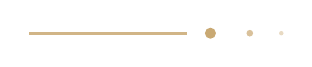
\begin{tikzpicture}
    \draw[GoldMain!60,line width=1.2pt] (0,0) -- (2.0,0);
    \fill[GoldMain!70] (2.3,0) circle (2pt);
    \fill[GoldMain!50] (2.8,0) circle (1.2pt);
    \fill[GoldMain!30] (3.2,0) circle (0.8pt);
  \end{tikzpicture}

  \vspace{0.8cm}

  % ── 主标题 ──
  {\Huge\bfseries\color{BlueDark} 分析学笔记\par}

  \vspace{0.6cm}
  % ── 作者 ──
  {\Large\color{BlueMain!70} Notes of Huginn Wong\par}

  \vspace{0.4cm}
  % ── 第二道装饰金线（两端圆点）──
  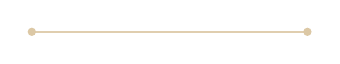
\begin{tikzpicture}
    \draw[GoldMain!40,line width=0.7pt] (0,0) -- (3.5,0);
    \fill[GoldMain!45] (0,0) circle (1.5pt);
    \fill[GoldMain!45] (3.5,0) circle (1.5pt);
  \end{tikzpicture}

  \vspace{0.8cm}
  % ── Fraktur 铭文 ──
  {\large\color{GoldMain!80} $\mathfrak{For}\quad\mathfrak{the}\quad\mathfrak{Worthy}$\par}

  \vspace{1.0cm}

%  % ── 封面图片区域（可选插入小图）──
%  \ifdefempty{\@coverimage}{
%    % 无图片：什么都不显示
%  }{
%    \begin{center}
%      \includegraphics[width=0.55\textwidth, height=3.5cm, keepaspectratio]{\@coverimage}
%    \end{center}
%    \vspace{0.3cm}
%  }
%
%  \vfill
%
%  % ── 日期 ──
%  {\large\color{BlueLight!65} \@date\par}
%  \vspace{0.8cm}
\end{minipage}

% ============================================================
%  第七层：右下角「出版社」小 logo（仿 Springer 风格）
% ============================================================
\begin{tikzpicture}[remember picture, overlay]
  \begin{scope}[shift={([xshift=-5.5cm, yshift=1.5cm]current page.south east)}]
    % 小房子
    \draw[BlueMain, line width=0.8pt] (0,0) rectangle (0.9,0.72);
    \draw[BlueMain, line width=0.8pt] (0,0.72) -- (0.45,1.08) -- (0.9,0.72);
    \draw[GoldMain, line width=0.5pt] (0.45,0.72) -- (0.45,1.08);
    \draw[BlueMain, line width=0.4pt] (0.23,0) -- (0.23,0.72);
    \draw[BlueMain, line width=0.4pt] (0.67,0) -- (0.67,0.72);
    % 屋顶金点
    \fill[GoldMain] (0.45,1.08) circle (1.5pt);
    \node[anchor=west, BlueMain, font=\footnotesize] at (1.1,0.32)
      {Produced by Huginn};
  \end{scope}
\end{tikzpicture}
% ============================================================
%  第八层：底部主封面图片 —— 与金色框左右对齐，位于小房子上方
% ============================================================
\ifdefempty{\@coverimage}{}{
	\begin{tikzpicture}[remember picture,overlay]
		\node[
		anchor=south west,
		inner sep=0pt,
		outer sep=0pt
		] at ([xshift=3.3cm,yshift=3.05cm]current page.south west)
		{
			\includegraphics[
			width=\dimexpr\paperwidth-4.8cm\relax
			]{\@coverimage}
		};
	\end{tikzpicture}
}


% ============================================================
%  第九层：散落装饰点（页面随机分布的数学点缀）
% ============================================================
\begin{tikzpicture}[remember picture,overlay]
  % 右中区域散点
  \fill[GoldMain!18] ([xshift=-3.0cm,yshift=-9.5cm]current page.north west) circle (1.0pt);
  \fill[BlueLight!18] ([xshift=-3.8cm,yshift=-9.8cm]current page.north west) circle (0.7pt);
  \fill[GoldMain!16] ([xshift=-2.5cm,yshift=-10.2cm]current page.north west) circle (0.8pt);
  % 右下方散点
  \fill[BlueMain!12] ([xshift=-4.0cm,yshift=3.5cm]current page.south west) circle (1.2pt);
  \fill[GoldMain!13] ([xshift=-5.5cm,yshift=4.0cm]current page.south west) circle (0.9pt);
  % 标题区附近轻微装饰
  \fill[GoldMain!20] ([xshift=14.5cm,yshift=-6.0cm]current page.north west) circle (1.0pt);
  \fill[BlueLight!16] ([xshift=14.0cm,yshift=-5.5cm]current page.north west) circle (0.6pt);
  \fill[GoldMain!18] ([xshift=15.0cm,yshift=-5.8cm]current page.north west) circle (0.8pt);
\end{tikzpicture}

\end{titlepage}
}
\makeatother

\addbibresource{bibliography/references.bib}

% ── 文档元信息与封面 ──
\title{分析学笔记}
\author{Huginn Wong}
\date{\today}
\coverimage{figure/分析封面.jpg}

\begin{document}

\makecover
	
	\frontmatter
	
	\chapter*{前言}
	\addcontentsline{toc}{chapter}{前言}
	
	这份笔记是我在学习分析学时所使用的笔记，今天是26年1月8日，完成了第一章，第三章除最后一节外的书写，快期末了，希望假期能把前7章的内容写完审完。
	
	\vspace{1cm}
	\begin{flushright}
		Huginn Wong\\
		2026年1月8日
	\end{flushright}
	
	今天是2026年的5月18日，在AI的辅助下，我已经完成了单变量分析的除了函数项数列与级数的大部分主题内容，在这一学期的行课结束后，我将完成函数项数列与级数那一章，接下来我的主要工作就是刷题与总结了，总结出的相应的内容会在后续逐步记在笔记里。之后还有代数的内容要整理，希望在假期期间我能够做足够的工作吧
		\vspace{1cm}
	\begin{flushright}
		Huginn Wong\\
		2026年5月18日
	\end{flushright}
	
	这里是2026年的6月4日晚上10点，改善了工作流之后，我们的产出效率得到了极大的提升，今天我完成了part1的主体部分的笔记，之后我们在刷题的过程中会不断的补充part1的内容，同时代数的笔记也快速的根上了进度，我想我或许可以开始继续学习更多的内容了
	\begin{flushright}
		Huginn Wong\\
		2026年6月4日
	\end{flushright}
	
	今天是2026年的7月6日上午8点15分，也是放假的第三天，经过三天的努力我已经把分析学Part的笔记中能够从我已经读过的书中的知识整理了出来，在接下来的时间里我需要逐渐的去读去做，谢惠民，于品和Baby Rudin，把那里面的一些想法和知识记录进来，这个学期的数分拿了一个不错的分数，希望下个学期在我的新工作流下，我能有更高的学习效率，取得更好的成绩
	\begin{flushright}
		Huginn Wong\\
		2026年7月6日
	\end{flushright}
	\newpage
	今天是2026年的8月13日晚上11点，经过半个假期的努力，我读完了Stein 的Fourier分析，接下来，我得读ODE和代数了。不得不说，线性代数里的一些东西我已经忘了，还是得融入血液啊。
	\begin{flushright}
		Huginn Wong\\
		2026年8月13日
	\end{flushright}
	\tableofcontents
	\newpage
	

	
	
	
	\mainmatter
	\setcounter{page}{1}
	
%\setpartimage{figure/part1封面图.png}
%\setpartintro{这一部分从 Peano 公理出发，建立实数系，进而研究数列与函数的极限、连续性和微积分基本理论，是全部分析学的根基所在。}
%\part{单变量分析学}
%\setcounter{chapter}{0}
%% ===== 第一部分：单变量分析学 / 第1章：实数理论——从Peano公理到实数的连续性 =====
% !TEX root = ../../main.tex
\setchapterimage{figure/chapter1封面图.png}
\setchapterintro{这一章我们的核心任务是从Peano公理开始，用Dedekind分割构建出我们要研究的实数域。另一种实数公理我想会在我的拓扑学的笔记中进行介绍，可以看到，以Peano公理为基础构建出的实数体系以直接利用实数公理的是可以互相嵌套的。另外，必须承认的是这一章关于集合的势的部分有很大的问题，可以先忽略掉这一节，我将在拓扑学笔记的第一章重新整理更严格的内容。}
	\chapter{实数理论——从Peano公理到实数的连续性}

% 第1节：朴素集合论
% !TEX root = ../../../main.tex
% 所属：第一部分：单变量分析学 / 第1章：实数理论——从Peano公理到实数的连续性
% 节：1.1 朴素集合论
% 正文按原文件顺序保存；由 ../chapter1.tex 调用。
\section{朴素集合论}
我们从朴素集合论开始，这由Cantor建立，在未严格公理化的基础上.请原谅我无法从公理化集合论开始.

\begin{definition}
	集合是具有某种性质的或具体或抽象事物汇集而成的一个整体，这些单一的事物称为集合的元素，用大写字母表示集合，小写字母表示元素.若 $x$ 是 $S$ 的元素则 $x \in S$
	
	我们把以集合为元素的集合称作族，用$\mathcal{A},\mathcal{B},\mathcal{T},\cdots$表示.
\end{definition}

\begin{example}
	集合有两种描述法，列举法和描述法.\\
	$\left\{1\right\},\left\{1,2,3,4\right\}$是列举法；$\left\{x:x>0,x\in\R\right\}$是描述法
\end{example}
\begin{definition}
	空集，是一个不包含任何元素的集合.用 $\varnothing$ 表示
	
\end{definition}
\begin{definition}
	S，T是两个集合，若
	
	\[x \in S \Rightarrow x \in T
	\]
	
	
	也就是说只要 $x \in S$ 就能推出 $x \in T$ .就称 $S$ 是 $T$ 的子集，记为 $S \subset T$
	显然 $x \in S \Rightarrow x \in S$ 故 $S \subset S$
	
\end{definition}
$\varnothing \subset S$ 的证明，用到了逻辑学中的空真原理，我们先对空真原理进行说明
\begin{prp}
	当一个条件语句（如果 P ，那么 Q ）的前提 P 为假，无论Q是真是假，这个条件语句本身必为真.
	

\end{prp}

	\begin{example}
		\begin{enumerate}
			\item 如果 $x$ 是一只独角兽，那么 $x$ 的角是金色的.
			分析：独角兽不存在，故此条件语句中前提是假的、根据空真原理，无法找到一只角不是金色的独角兽来反驳，因此这个条件语句是空真的.
			\item $x\in\R$若$x^2<0$那么$x=23$，这个命题是真的.因为$x\in\R$只能$x^2\geqslant0$.
		\end{enumerate}
\end{example}

这样，我们证明 $\varnothing \subset S$.
根据 $\subset$ 的定义 $\quad x \in \varnothing \Rightarrow x \in S$
,而 $x \in \varnothing$ 假，根据空真原理 $\varnothing\subset S$ 成立.
\begin{definition}
	集合 $S$ ，$T$ 的并，记为 $S \cup T$
	
	$$
	S \cup T=\{x: x \in S \text { 或} x \in T\}
	$$
	
	$S, T$ 的交，记为 $S \cap T$
	
	$$
	S \cap T=\left\{x:x \in S \text { 且 } x \in T\right\}
	$$
	
	$S, T$ 的差，记为 $S \setminus T$
	
	$$
	S\setminus T=\{x :x \in S \text { 且 } x \notin T\}
	$$
	
	$S$ 的补，记为 $S_U^C$ ，$U$ 为全集，有时省略下角标 $U$ ，用 $S^C$ 表示.
	\[S_U^C=\left\{ x:x \in U \text{且} x \notin S\right\}\]
	
	
\end{definition}

\begin{proposition}
	\begin{enumerate}
		\item $A \cup B=B \cup A, A \cap B=B \cap A$ 
		\item$A \cup(B \cup D)=(A \cup B) \cup D, A \cap(B \cap D)=(A \cap B) \cap D$
		\item$A \cap(B \cup D)=(A \cap B) \cup(A \cap D), A \cup(B \cap D)=(A \cup B) \cap(A \cup D)$
	\end{enumerate}

\end{proposition}
\begin{center}
	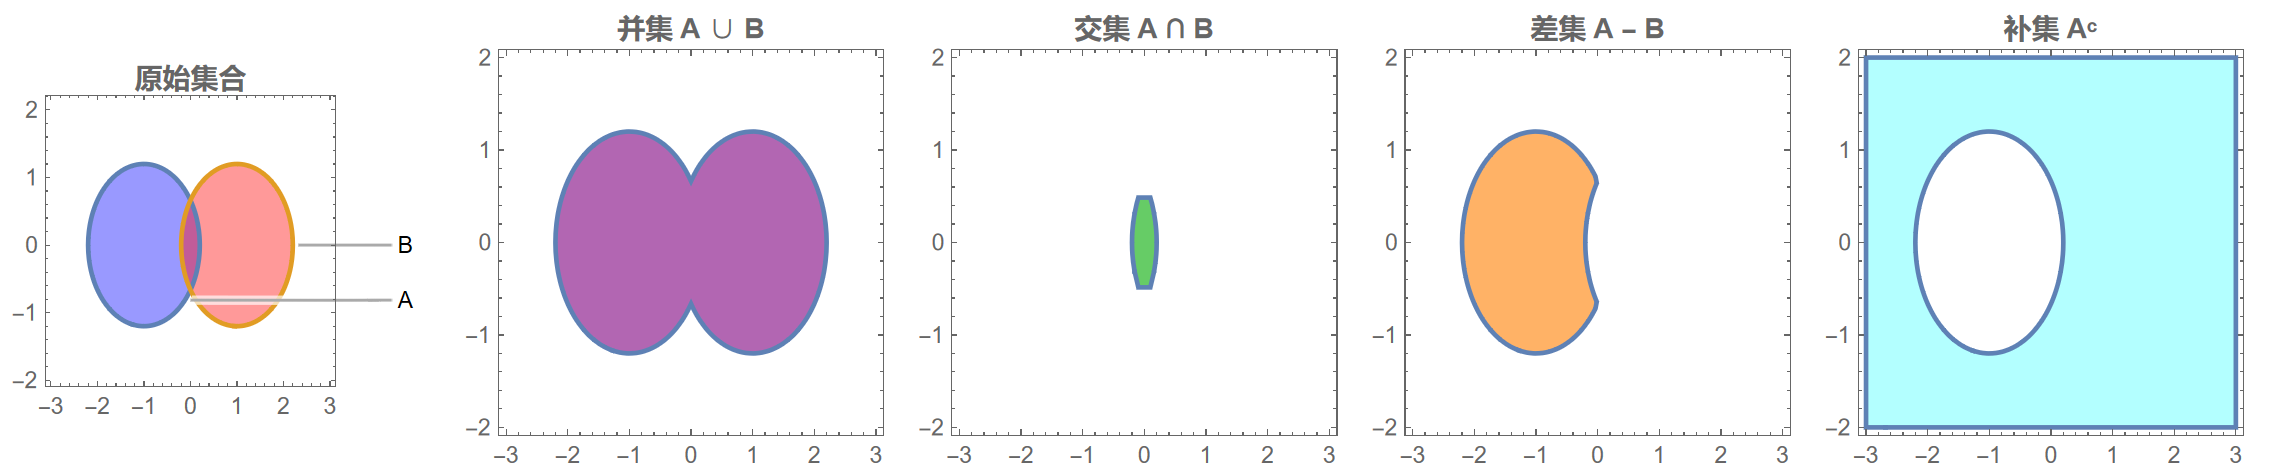
\includegraphics[width=\linewidth]{figure/C1/96aac8f9ecba0c3ccf651dd1b1ab3b43}
	\label{fig:96aac8f9ecba0c3ccf651dd1b1ab3b43}
\end{center}

\begin{proof}
	1，2是显然的，下证3\\
	先证 $A \cap(B \cup D)=(A \cap B) \cup(A \cap D)$
	\\（i）$A \cap(B \cup D) \subset(A \cap B) \cup(A \cap D)$\\
	设 $x \in A \cap(B \cup D) \Rightarrow x \in A$ 并且 $x \in B$ 或 $x \in D \Rightarrow x \in A \cap B$ 或者 $x \in A \cap D \Rightarrow x \in(A \cap B) \cup(A \cap D) \rightarrow A \cap(B \cup D) \subset(A \cap B) \cup(A \cap D)$ \\（ii）$A \cap(B \cup D) \supset( A \cap B) \cup(A \cap D)$\\
	$x \in(A \cap B) \cup(A \cap D) \Rightarrow x \in A$ 且 $x \in B$ 或 $x \in A$ 且 $x \in D \Rightarrow x$ 必 $\in A, x \in B$ 或 $x \in D \Rightarrow x \in A \cap(B \cup D) \rightarrow A \cap(B \cup D) \supset(A \cap B) \cup(A \cap D)$\\故 $A \cap(B \cup D)=(A \cap B) \cup(A \cap D)$
	
	再证 $A \cup(B \cap D)=(A \cup B) \cap(A \cup D)$
	
	$x \in A \cup(B \cap D) \Leftrightarrow x \in A$ 或$x \in B$ 并且 $x \in D \Leftrightarrow x \in A$ 或 $x \in B$ 且 $x \in A$ 或 $x \in D$
	$\Leftrightarrow x \in A \cup B$ 且 $x \in A \cup D \Leftrightarrow x \in(A \cup B) \cap(A \cup D)$
	
	
\end{proof}
\begin{proposition}
	De Morgan 公式
	$$
	(A \cup B)^C=A^C \cap B^C \quad(A \cap B)^C=A^C \cup B^C
	$$
	\label{demordan}
\end{proposition}

\begin{proof}
	先证 $(A \cup B)^C=A^C \cap B^C$
	
	$x \in(A \cup B)^c \Leftrightarrow x \notin A \cup B \Leftrightarrow x \notin A$ 且 $x \notin B \Leftrightarrow x \in A^C$ 且 $x \in B^C \Leftrightarrow x \in A^C \cap B^C$
	
	
	故 $(A \cup B)^c=A^C \cap B^C$
	
	
	
	再证明 $(A \cap B)^C=A^C\cup B^C$
	
	$ x \in(A \cap B)^C \Leftrightarrow x \notin A \cap B \Leftrightarrow x \notin A\text{或}x \notin B \Leftrightarrow x \in A^C\cup B^C$
	
	故 $(A \cap B)^C=A^C \cup B^C$
\end{proof}
\begin{corollary}
	设$\{S_{\alpha}\}$是$M$中的一组集，$\mathcal{A}$是一个指标集，那么
	\[ (\bigcap_{\alpha\in\mathcal{A}}S_{\alpha})^{C}=\bigcup_{\alpha\in\mathcal{A}}S_{\alpha}^{C}\qquad(\bigcup_{\alpha\in\mathcal{A}}S_{\alpha})^{C}=\bigcap_{\alpha\in\mathcal{A}}S_{\alpha}^{C} \]
\end{corollary}
\begin{proposition}
	\begin{enumerate}
		\item $A\setminus\varnothing=A$,$A\setminus  A=\varnothing$
		
		\item$U$是全集，$A\setminus  U=\varnothing$,$U\setminus  A=A^C$
		\item$A\setminus  B=A \cap B^c$
		\item$
		A\setminus  (B \cap C)=(A\setminus  B) \cup(A\setminus  C)
		$
		一般的，有$$X\setminus  \bigcap U_{\alpha}=\bigcup(X\setminus  U_{\alpha})$$
		
		\item$A\setminus  (B \cup C)=(A\setminus  B) \cap(A\setminus  C)$
		一般的，$$X\setminus  \bigcup U_{\alpha}=\bigcap(X\setminus  U_{\alpha})$$
		
		
		\item$A\setminus  B=\varnothing$ 当且仅当 $A \subset B$
		\item 如果 $A \subseteq B$ ，那么对于任意集合 C，有 $A\setminus  C \subseteq B\setminus  C$
		
		如果 $A \subseteq B$ ，那么 $C\setminus  B \subseteq C\setminus  A$
		
	\end{enumerate}
\end{proposition}
\begin{proof}
	\begin{enumerate}
		\item （a）$A\setminus\varnothing=A$
		
		任取 $x$ ， $x \in(A\setminus\varnothing) \Longleftrightarrow(x \in A) \textbf{且}(x \notin \varnothing) \Longleftrightarrow x \in A$ .因为 $x \notin \varnothing$ 恒真.
		所以 $A\setminus \varnothing=A$ .
		
		（b）$A\setminus A=\varnothing$
		
		任取 $x$,
		$
		x \in(A\setminus A) \Longleftrightarrow(x \in A) \textbf{且}(x \notin A) 
		$
		
		
		但 $x \in A$ 与 $x \notin A$ 不可能同时成立，故 $A\setminus A$ 不含任何元素，即 $A\setminus A=\varnothing$ 
		
		\item（a）$A\setminus U=\varnothing$
		
		任取 $x$ ，$x \in(A\setminus U) \Longleftrightarrow(x \in A) \textbf{且}(x \notin U) $
		
		因为 $U$ 是全集，所以 $x \notin U$ 恒假.
		故 $A\setminus U$ 不含任何元素，即 $A\setminus U=\varnothing$ 
		
		（b）$U\setminus A=A^c$
		
		任取 $x$，$x \in(U\setminus A) \Longleftrightarrow(x \in U) \textbf{且}(x \notin A) \Longleftrightarrow \text { True } \textbf{且}(x \notin A) \Longleftrightarrow x \notin A \Longleftrightarrow x \in A^C$
		\item
		
		任取 $x$ ，
		
		$
		x \in(A\setminus B) \Longleftrightarrow(x \in A) \textbf{且}(x \notin B) \Longleftrightarrow(x \in A) \textbf{且}\left(x \in B^C\right) \Longleftrightarrow x \in\left(A \cap B^C\right)
		$
		
		
		所以 $A\setminus B=A \cap B^C$ .
		\item 由3和\ref{demordan}易得
		
		\item 由3和\ref{demordan}易得
		\item
		 $\Rightarrow$ :假设 $A\setminus B=\varnothing$ .要证 $A \subset B$ .
		任取 $x \in A$ .若 $x \notin B$ ，则 $x \in A\setminus B$ ，与 $A\setminus B=\varnothing$ 矛盾.故 $x \in B$ .
		所以 $A \subset B$ .
		
		$\Leftarrow$ :假设 $A \subset B$ .要证 $A\setminus B=\varnothing$ .
		任取 $x \in A\setminus B$ ，则 $x \in A$ 且 $x \notin B$ .但 $A \subset B$ 意味着 $x \in A \Rightarrow x \in B$ ，矛盾.故不存在这样的 $x$ ，即 $A\setminus B=\varnothing$ .
		
		所以 $A\setminus B=\varnothing \Longleftrightarrow A \subset B$ .
		
		\item
		
		（a）如果 $A \subset B$ ，那么对于任意集合 $C$ ，有 $A\setminus C \subset B\setminus C$
		假设 $A \subset B$ .
		任取 $x \in A\setminus C$ ，则 $x \in A$ 且 $x \notin C$ .
		由 $x \in A$ 和 $A \subset B$ 得 $x \in B$ .
		
		所以 $x \in B$ 且 $x \notin C$ ，即 $x \in B\setminus C$ .
		故 $A\setminus C \subset B\setminus C$ .
		
		（b）如果 $A \subset B$ ，那么 $C\setminus B \subset C\setminus A$
		假设 $A \subset B$ .
		任取 $x \in C\setminus B$ ，则 $x \in C$ 且 $x \notin B$ .
		由 $A \subset B$ 和 $x \notin B$ 可得 $x \notin A$（因为若 $x \in A$ 则 $x \in B$ ，矛盾）.
		
		所以 $x \in C$ 且 $x \notin A$ ，即 $x \in C\setminus A$ .
		故 $C\setminus B \subset C\setminus A$ .
	\end{enumerate}
\end{proof}
我们有一下记号
	\[ S=E_1 \cup E_2 \cup \cdots E_n=\bigcup_{x=1}^n E_x\quad \bigcup_{x=1}^{+\infty} E_x\quad \bigcup_{x \in A} E_x \]
	\[T=E_1 \cap E_2 \cap \cdots \cap E_n=\bigcap_{x=1}^n E_x \quad \bigcap_{x=1}^{+\infty} E_x\quad \bigcap_{x \in A} E_x\]	
	
	
这种集合的运算性质，说明了集合构成的类加上交并补的运算可以形成一个代数结构，也就是布尔代数.
\begin{definition}
	对A，B两者的Descartes积定义为
	
	$$
	A \times B:=[(x, y): x \in A, y \in B]
	$$
	
	
	对 $A_1, \cdots, A_n$
	
	$$
	A_1 \times \cdots \times A_n:=\left[\left(x_1, \cdots, x_n\right): x_1 \in A_1, \cdots, x_n \in A_n\right]
	$$
\end{definition}
\newpage
%
% 第2节：代数结构初步
% !TEX root = ../../../main.tex
% 所属：第一部分：单变量分析学 / 第1章：实数理论——从Peano公理到实数的连续性
% 节：1.2 代数结构初步
% 正文按原文件顺序保存；由 ../chapter1.tex 调用。
\section{代数结构初步}


从自然数向有理数扩张的过程，是代数结构由低级到
高级的过程，这里对代数结构进行初步的说明.
\begin{definition}
	代数结构，是一个集合，配上一个或多个运算，并且满足一定的公理 .运算的一般形式有加法，乘法，数乘，甚至交并非的集合运算.
\end{definition}


\begin{definition}简单代数结构树状图
	
	
\end{definition} 
\begin{tikzpicture}[
	node distance=1cm and 0.8cm,  % 减小节点间距
	algNode/.style={
		draw=black,
		thick,
		rounded corners=4pt,     % 减小圆角
		minimum width=2.5cm,     % 减小宽度
		minimum height=0.8cm,    % 减小高度
		text width=2.3cm,        % 减小文本宽度
		align=center,
		font=\scriptsize         % 使用更小的字体
	},
	arrow/.style={
		-Stealth,
		thick,
		line width=0.6pt        % 减细箭头
	}
	]
	
	% 定义节点
	\node[algNode] (magma) {群胚\\集合 + 运算+封闭性};
	\node[algNode, below=of magma] (semi) {半群\\+ 结合律};
	\node[algNode, below=of semi] (monoid) {幺半群\\+ 单位元};
	\node[algNode, below left=of monoid] (group) {群\\+ 逆元};
	\node[algNode, below right=of monoid] (ring) {环\\加法阿贝尔群\\乘法半群或幺半群};
	\node[algNode, below=of group] (abelian) {阿贝尔群\\+ 交换律};
	\node[algNode, below=of ring] (commRing) {交换环\\乘法交换律};
	\node[algNode, below=of commRing] (domain) {整环\\无零因子+单位元};
	\node[algNode, below=of domain] (field) {域\\乘法逆元存在\\加法，乘法，分配公理};
	
	% 绘制箭头
	\draw[arrow] (magma) -- (semi);
	\draw[arrow] (semi) -- (monoid);
	\draw[arrow] (monoid) -- (group);
	\draw[arrow] (monoid) -- (ring);
	\draw[arrow] (group) -- (abelian);
	\draw[arrow] (ring) -- (commRing);
	\draw[arrow] (commRing) -- (domain);
	\draw[arrow] (domain) -- (field);
	
\end{tikzpicture}
\newpage

%
% 第3节：Peano公理与$\N$自然数集的构建
% !TEX root = ../../../main.tex
% 所属：第一部分：单变量分析学 / 第1章：实数理论——从Peano公理到实数的连续性
% 节：1.3 Peano公理与$\N$自然数集的构建
% 正文按原文件顺序保存；由 ../chapter1.tex 调用。
\section{Peano公理与$\N$自然数集的构建}
\begin{axiom}Peano公理\label{peano}
	\begin{enumerate}
		\item 0 是自然数.
		\item 每一个自然数 $n$ 都有且仅有一个后继 $S(n)$ ，且 $S(n)$ 也是自然数.
		
		\item 0不是任何自然数的后继.
		\item 不同的自然数有不同的后继.
		\item P(n)是一个关于自然数的命题.若 $P(0)$ 成立，对任意自然数 $k$ ，如果 $P(k)$ 能推出 $P(S(k))$ 成立，那么 $P(n)$ 对所有自然数成立.
		
		
	\end{enumerate}
	
\end{axiom}

现在 $0$ 是那个起始的数，$S(0)$ 称为 $1, S(S(0))$ 称为 2 … 以此类推得 $0,1,2,3,4$ ．．把这些不断后继得到的东西构成一个无限的集合.这个集合就是自然数集$\N$.

这样，我们就把自然数这个直观的概念建立在了不依赖直观的公理上.
\begin{definition}设$a,b\in \N$，定义$\N$上的二元运算
	\begin{itemize}
		\item 加法 
		\begin{enumerate}
			\item $ a+0=a$ 任何数加 0 等于它本身.
			\item $a+S(b)=S(a+b) $一个数加另一个数的后继，等于这两个数和的后继.
		\end{enumerate}
		\item 乘法
		\begin{enumerate}
			\item $a \cdot 0=0$
			\item$ a \cdot S(b)=a \cdot b+a$
		\end{enumerate} 
	\end{itemize}
	
	
	
\end{definition}

在这种加法和乘法的定义下，自然数集对加法能构成交换幺半群，对乘法同样.

现在，我们进述冯诺依曼对Peano公理的集合论叙述.
\begin{axiom}Peano公理的集合论叙述\label{peano2}
	\begin{enumerate}
		\item $0:=\varnothing$
		\item$S(n):=n \cup\left\{n\right\}$\\
		这样 $0:=\varnothing, 1:=S(0)=\varnothing \cup\left\{\varnothing\right\}=\left\{\varnothing\right\}=\left\{0\right\}$,
		$2:=S(1)=\left\{\varnothing\right\} \cup\{\left\{\varnothing\right\}\}=\left\{\varnothing,\left\{\varnothing\right\}\right\}=\left\{0,1\right\}\ldots$
		\item 无穷公理： $\exists$ 集合 $I$ 使得 $\varnothing\in I\text{且}x\in I\rightarrow S(x)\in I$.就称$I$为归纳集.
	\end{enumerate}
	取 $\N:=\bigcap\left\{I:I\text{是一个归纳集}\right\}$，也就是说$\N$是最小的归纳集.
\end{axiom}



说明取交的原因，集 $I=\left\{0,1,2,3,4\ldots\text{苹果},\text{苹果}^+,\text{苹果}^{++}\ldots\right\}$, 定义 0 ，苹果为起始，$S$（苹果）$=\text{苹果}^+$  ，$I$亦是归纳集，这个$I$是丑陋不堪的，不纯的，故取所有$I$的交，只留下最小的那个. \[\left\{0,1,2,3\ldots\right\}\]
现在，我们用\ref{peano2}反验\ref{peano}
\begin{proposition}
		由\ref{peano2}可以推出\ref{peano}.
\end{proposition}

\begin{proof}
	\begin{enumerate}
		\item $0=\varnothing \in$ 每一个归纳集，故 $0=\varnothing \in \bigcap I$ 成立.
		\item  $n \in \N$ 则n属于每一个归纳集，那么每一个$I$包含 $S(n)$ .
		故 $S(n) \in \N \quad$ 成立.
		\item $S(n)=n \cup\left\{n\right\}$ 包含元素 $n$ ，而 $0=\varnothing$ 不含任何元素,
		$S(n)$ 不可能是空集 ,成立.
		\item 对 $m, n \in \mathbb{N}$ ，假设 $S(m)=S(n) \Rightarrow m \cup\left\{m\right\}=n \cup\left\{n\right\}$,
		若 $m \in n$，则由 $\mathbb{N}$ 中元素的传递性（每个自然数等于其所有元素之并的子集）有 $m \subseteq n$；
		若 $m = n$，则显然 $m \subseteq n$. 无论何种情形 $m \subseteq n$.
		对称地 $n \subseteq m$，故 $m=n$ 成立.
		\item 考虑集合 $A=\left\{n \in \mathbb{N}: P(n)\text{为真}\right\}$ \\
		$P(0)$ 真，故 $0 \in A \quad$ ,若 $P(k)$ 真则 $P(S(k))$ 真，故 $k \in A \rightarrow S(k) \in A$故 $A$ 是一个归纳集 $\Rightarrow \mathbb{N} \subset A$ 又 $A \subset \N \Rightarrow A=\mathbb{N} \Rightarrow$ 对所有 $n \in \mathbb{N}$ 成立
	\end{enumerate}
\end{proof}
现在，任何关于数的理论都建立在了集合论的基础上.而我们的集合论是公理化的，严谨的，我们的数学大厦就有了坚实的地基.

%
% 第4节：等价关系，商集与$\Z$整数的构建
% !TEX root = ../../../main.tex
% 所属：第一部分：单变量分析学 / 第1章：实数理论——从Peano公理到实数的连续性
% 节：1.4 等价关系，商集与$\Z$整数的构建
% 正文按原文件顺序保存；由 ../chapter1.tex 调用。
\section{等价关系，商集与$\Z$整数的构建}
\begin{definition}
	定义一个关系是等价关系$\sim$若它满足如下条件
	\begin{enumerate}
		\item 自反性：$A \sim A$
		\item 对称性：若 $A \sim B$ 则 $B \sim A$
		\item 传递性：若 $A \sim B$ 且 $B \sim C$ 则 $A \sim C$
	\end{enumerate}
	
	
\end{definition}
\begin{definition}
	在一个集合$X$上定义一个等价关系$\sim$.
	对某一元素 $a, \left[a\right]$ 定义成所有与 $a$ 等价的元素构成的集合，也就是说
	
	$$
	[a]=\left\{x \in X: x \sim a\right\}
	$$
	
	$\left[a\right]$被称作 $a$ 的等价类.
\end{definition}

\begin{lemma}
	等价类 $[a], a \in X$ ，$[a]$ 有以下三条性质.
	\begin{enumerate}
		\item $a \in[a]$
		\item $b \in[a]$ 则 $[a]=[b]$
		\item 任意两个等价类 $[a],[b]$ 要么 $[a]=[b]$ 要么 $[a]\cap[b]=\varnothing$
	\end{enumerate}
\end{lemma}
\begin{proof}
	\begin{enumerate}
		\item $a \sim a$
		\item 任取 $x\in[a]$，即 $x\sim a$. 由 $b\in[a]$ 知 $b\sim a$，由对称性 $a\sim b$，传递性得 $x\sim b$，故 $x\in[b]$，即 $[a]\subseteq[b]$. 同理 $[b]\subseteq[a]$，故 $[a]=[b]$
		\item 若 $[a] \cap[b] \neq \varnothing$ ,设 $x \in[a] \cap[b]$ 则 $a\sim x,b\sim x,a\sim b$, 
		$[a]=[b]$
	\end{enumerate}
\end{proof}
\begin{definition}
	＂$\sim$＂是 $X$ 上的一个等价关系.由＂$\sim$＂确定的等价类构成的集合，称为 $X$ 关于 $\sim$ 的商集，记为 $X / \sim$
	
	$$
	X / \sim=\{[a]: a \in X\}
	$$
\end{definition}
现在，利用商集的概念，我们可以从自然数上构造整数.
\begin{construction}整数的构造
	$$
	\text { 令 } S=\{(a,b): a,b \in \mathbb{N}\}
	$$
	
	（虽然我们尚未定义＂减法＂，为了方便理解 $(a, b)\Leftrightarrow a-b$）\\
	在 $S$ 上定义$\sim$
	\[(a, b) \sim(c, d) \quad\text{iff}\quad a+d=b+c\]	
	
	$$
	[a+d=b+c \Leftrightarrow a-b=c-d]
	$$
	这样
	
	$$
	\Z:=S/\sim
	$$
	每个等价类 $[a, b]$ 是一个整数.
\end{construction}   



\begin{proof}
	现验证$\sim$是等价关系.
	\begin{enumerate}
		\item  自反性 $a+b=b+a \quad(a, b) \sim(a, b)$
		\item 对称性 $(a, b) \sim(c, d) \Leftrightarrow a+d=b+c \Leftrightarrow c+b=d+a \Leftrightarrow (c, d) \sim(a, b)$
		\item 
		传递性 $(a, b) \sim(c, d), ( c, d) \sim(e, f) \Leftrightarrow$
		$$
		a+d=b+c, c+f=d+e \Leftrightarrow a+f=b+e \Leftrightarrow(a, b) \sim(e, f)
		$$
	\end{enumerate}
\end{proof}

现对 $\Z$ 上的运算进行定义.\\
\begin{definition}
	加法 $[(a, b)]+[(c, d)]:=[(a+c, b+d)]$\\
	加法逆元 $-[(a, b)]:=[(b, a)]$\\
	减法 $[(a, b)]-[(c, d)]:=[(a+d, b+c)]$\\
	乘法 $[(a, b)] \cdot[(c, d)]:=[(a c+b d, a d+b c)]$\\
	通常情况下 $[(n, 0)]$ 记作 $n \quad \Rightarrow \mathbb{N} \subset \mathbb{Z}$\\
	$[(0, n)]$ 记作 $-n$\\
	$[(a,b)]$记作$a-b$\\
\end{definition}

这样，我们就严格的构造出了整数集，并且定义了其上的运算.\\
$(\Z,+)$ 是阿贝尔群，
$(\mathbb{Z}, +, \cdot)$ 是交换环\\
\begin{example}
	-2 对应 $[(3,5)],[(1,3)]$ 等,
	-4 对应 $[(1,5)],[(6,10)]$ 等
\end{example}


%
% 第5节：$\Q$有理数的构建
% !TEX root = ../../../main.tex
% 所属：第一部分：单变量分析学 / 第1章：实数理论——从Peano公理到实数的连续性
% 节：1.5 $\Q$有理数的构建
% 正文按原文件顺序保存；由 ../chapter1.tex 调用。
\section{$\Q$有理数的构建}
\begin{construction}有理数的构建
	$$
	S=\left\{(a, b): a, b \in \mathbb{Z}\text{且}b\ne0\right\}
	$$
	
	
	在 $S$ 上定义 $\sim$ 关系
	\[(a, b) \sim(c, d) \text { iff } a d=b c\]
	\[\Q:=S/\sim\]
	
\end{construction}



现验证 $\sim$ 是等价关系
\begin{proof}
	\begin{enumerate}
		\item 自反性 $(a, b) \sim(a, b) \Leftrightarrow a b=b a$
		\item   对称性 $(a, b) \sim ( c, d) \Leftrightarrow a d=b c \Leftrightarrow c b=d a$
		\[\text{故}(c, d) \sim(a, b)\]
		
		\item  传递性 $(a, b) \sim(c, d)$ 且 $(c, d) \sim(e, f)$
		
		$$
		\begin{aligned}
			& \Leftrightarrow a d=b c \text { 且 } c f=d e \\
			& \Leftrightarrow a f=b e \Leftrightarrow(a, b) \sim(e, f)
		\end{aligned}
		$$
		
	\end{enumerate}
\end{proof}
每个等价类$[(a, b)]$ 是一个有理 数.

\begin{definition}$\Q$上的运算\\
	加法 $[(a, b)]+[(c, d)]:=[( a d+b c, b d)]$\\
	加法逆元 $-[(a, b)]:=[(-a, b)]$ 或$[(a,-b)]$\\
	乘法 $[(a, b)] \cdot[c, d]:=[(a c, b d)]$\\
	乘法逆元 $[(a, b)]^{-1}=[(b, a)]$,其中$a,b\ne0$
\end{definition}

在$\Q$上$[(a, b)]$ 记作 $\dfrac{a}{b} \quad$


显然 $[(n, 1)]=n \in \mathbb{Z} \Rightarrow \mathbb{Z} \subset\Q$

$\Q$是一个数域

\begin{example}
	$$\dfrac{1}{2}=[(2,4)]=[(3,6)]=\cdots$$
	$$\dfrac{3}{5}=[(6,10)]=[(3,5)]=\cdots$$
\end{example}

%
% 第6节：数域
% !TEX root = ../../../main.tex
% 所属：第一部分：单变量分析学 / 第1章：实数理论——从Peano公理到实数的连续性
% 节：1.6 数域
% 正文按原文件顺序保存；由 ../chapter1.tex 调用。
\section{数域}
我们在这里，对域的概念加以重申.
\begin{definition}\label{1.6.1}
	一个三元组$(\F,+,\cdot)$若满足以下 11 条公理，则被称为\textbf{域}:
	\begin{enumerate}
		\item $\forall a, b \in \mathbb{F} \quad a+b \in \mathbb{F}$
		\item $\forall a, b \in \mathbb{F} \quad a+b=b+a$
		\item $\forall a, b, c \in \mathbb{F} \quad(a+b)+c=a+(b+c)$
		\item $\exists 0 \in \mathbb{F}$ 使得$a+0=a$
		\item $\exists-a \in \mathbb{F}$ 使得$-a+a=0$
		\item $\forall a, b \in \mathbb{F} \quad a b \in \mathbb{F}$
		\item $\forall a, b \in \mathbb{F} \quad a b=b a$
		\item $\forall a, b, c \in \mathbb{F} \quad(a b) c=a(b c)$
		\item $\exists 1 \in \mathbb{F}$使得 $a \cdot 1=a$
		\item $\forall a \in \F, a \neq 0 \Rightarrow \exists a^{-1} \in \F$ 使得 $a \cdot a^{-1}=1$
		\item $\forall a, b, c \in \mathbb{F} \quad(a+b) c=a \cdot c+b \cdot c$
	\end{enumerate}
	$1\sim5$称为加法公理记为$(A1)\sim(A5)$,$6\sim10$称为乘法公理记为$(M1)\sim(M5)$，11称为分配公理，记为(D)
\end{definition}
事实上，对四则运算封闭，有交换律，结合律，分配律就为域.
\begin{proposition}\label{1.6.2}
	$(A1)\sim(A5)$中有以下命题成立
	\begin{enumerate}
		\item $x+y=x+z \Rightarrow y=z$
		\item $x+y=x \Rightarrow y=0$
		\item$x+y=0 \Rightarrow y=-x$
		
		\item $-(-x)=x$
	\end{enumerate}
\end{proposition}
\begin{proof}
	$$
	\begin{aligned}
		y & =0+y=(-x+x)+y=-x+(x+y) \\
		& =-x+(x+z)=(-x+x)+z=0+z=z .
	\end{aligned}
	$$
	
	
	得证．
	
	在1中取 $z=0$ 就是2，在1中取 $z=-x$ 就是3，
	因 $-x+x=0$ ，3（用 $-x$ 代替 $x, x$ 代替 $y$ ）就能产生出4.
\end{proof}
\begin{proposition}
	$(M1)\sim(M5)$中有以下命题成立
	\begin{enumerate}
		\item $x \neq 0$ 且 $x y=x z \Rightarrow y=z$
		\item$x \neq 0$ 且 $x y=x \Rightarrow y=1$
		\item$x \neq 0$ 且 $x y=1 \Rightarrow y=\dfrac{1}{x}$
		\item $x \neq 0 \Rightarrow\left(x^{-1}\right)^{-1}=x$
	\end{enumerate}
	
\end{proposition}
\begin{proof}
	类似\ref{1.6.2}，省略
\end{proof}
\begin{proposition}\label{1.6.4}
	$\forall x, y, z \in \mathbb{F}$ ，以下命题成立
	\begin{enumerate}
		\item  $0 x=0$
		\item $x \neq 0$ 且 $y \neq 0$ 那么 $x y \neq 0$
		\item $(-x) y=-(x y)=x(-y)$
		\item $(-x)(-y)=x y$
	\end{enumerate} 
\end{proposition}
\begin{proof}
	$0 x+0 x=(0+0) x=0 x$ ．因此,有 $0 x=0$ ，而1成立
	
	
	设 $x \neq 0, y \neq 0$ 而 $x y=0$ ．于是由（a）能推出
	
	$$
	1=\left(\dfrac{1}{y}\right)\left(\dfrac{1}{x}\right) x y=\left(\dfrac{1}{y}\right)\left(\dfrac{1}{x}\right) 0=0
	$$
	
	
	矛盾．于是2成立．
	
	
	3中前一等式，可由
	
	$$
	(-x) y+x y=(-x+x) y=0 y=0
	$$
	
	
	得来；3的后半可用同样方法证明．
	
	最后，由3得
	
	$$
	(-x)(-y)=-[x(-y)]=-[-(x y)]=x y 
	$$
\end{proof}




%
% 第7节：序公理，有理数的阿基米德性和稠密性，上下确界
% !TEX root = ../../../main.tex
% 所属：第一部分：单变量分析学 / 第1章：实数理论——从Peano公理到实数的连续性
% 节：1.7 序公理，有理数的阿基米德性和稠密性，上下确界
% 正文按原文件顺序保存；由 ../chapter1.tex 调用。
\section{序公理，有理数的阿基米德性和稠密性，上下确界}
\begin{axiom}
	在集$S$上定义一种关系，名为序,记作$<$有如下性质
	
	（i）若 $x, y \in S$ ，那么在
	
	$$
	x<y \quad x=y \quad y<x
	$$
	
	
	三者中必备其一
	
	
	（ii）$x, y, z \in S \quad x<y$ 且 $y<z \Rightarrow x<z$
	
	有时用 $x>y$ 代替 $y<x$
	
	\label{1.7.1}
\end{axiom}
\begin{definition}$\N$,$\Z$,$\Q$上序的定义
	\begin{enumerate}
		\item$\N$定义序：对 $n \in \mathbb{N}$ ，规定 $S(n)>n$ 如此就定义了 $\mathbb{N}$ 上的序关系
		
		$0$ 不是任何自然数的后继，故 $0=\min\N$ 
		\item $\Z$定义序：$\Z:=\left\{[(a,b)]:a,b\in\N\right\}$
		
		若 $[(a, b)]>[(c, d)]$ 则 $a+d>b+c$
		\item 	$\Q$定义序:$\left\{[(a,b)]:a,b\in\Z\text{且}b\ne0\right\}\quad(a, b):=\dfrac{a}{b}$
		
		若 $[(a, b)]>[(c, d)]$ 则 $a d > b c$
	\end{enumerate}
	
	显然地，我们定义的序关系满足\ref{1.7.1}中的（i），（ii）
	
\end{definition}
\begin{definition}
	具有序关系 $<$ 的一个集合 $A$ 称为良序的，如果 $A$ 的任意非空子集有一个最小元.
\end{definition}
\begin{theorem}良序定理
	
	若 $A$ 是一个集合，则存在 $A$ 上的一个序关系，使 $A$ 成为一个良序集.
\end{theorem}

这个定理是1904年由 Zermelo 证明的，曾震动了数学界，并对其证明的正确性展开大量辩论.对于任意不可数集，没有一个将其良序化的构造性程序就引起了许多怀疑.在进一步分析这个证明时，我们发现只有一处可能有点问题，就是在构造的过程中包含着无穷多次选择，也就是说其做法包含了选择公理.

一些数学家曾经拒绝把选择公理作为一个结果，多少年来每涉及一个新定理就要提出这个问题：它的证明是否涉及选择公理？因为一个定理的证明中如果使用了选择公理，便会被认为基础不稳固.一般说来，时下的数学家大都已经不再有这样的烦恼了.他们把选择公理作为集合论中的一个合适的假定，良序定理也就随之得以被承认.

选择公理蕴涵良序定理的证明过于冗长（虽然不是特别困难），而且主要是逻辑学家的兴趣所在，我们略去其证明.我们承认良序定理，读者也可以将其视作另外的一个公理！

\begin{axiom}选择公理
	
	给定由两两无交的非空集合构成的一个族 $\mathcal{A}$ ，存在一个集合 $C$ ，使得 $C$ 与 $\mathcal{A}$ 的每一个元素恰好有一个公共元，即对于每一个 $A \in \mathcal{A}$ ，集合 $C \cap A$ 包含着唯一的一个元素．
\end{axiom}
\begin{definition}
	高斯取整$\left[a\right]$，是不大于 $a $的，最小的那个整数.
	
\end{definition}
\begin{proposition}
	$\Q$上的阿基米德性
	
	$x, y \in \mathbb{Q}$ 且 $x>0 \quad$ 那么 存在 $n \in \mathbb{Z}_{+} \quad$ 使
	\[	n x>y\]\label{1.7.7}
\end{proposition}

\begin{proof}
	取 $n=\left[|\dfrac{y}{x}|\right]+1$,得证.    	
	
\end{proof}
\begin{definition}\label{有序域}
	有序域是一个域 $\F$ ，又是合于下列两条件的有序集
	
	（i）当 $x, y, z \in F$ 且 $y<z$ 时，$x+y<x+z$ ；
	
	（ii）如果 $x, y \in F, x>0$ 且 $y>0$ ，那么 $x y>0$ ．
	
	如果 $x>0$ ，就说 $x$ 是正的；如果 $x<0$ ，就说 $x$ 是负的．
	
	例如，$\Q$ 是有序域．
	
\end{definition}

一个满足\ref{1.7.1}和\ref{1.7.7}的域称为 Archimedean有序域.



\begin{proposition}
	在每个有序域中，下面几条叙述都正确：
	
	（a）如果 $x>0$ ，那么 $-x<0$ ；反过来也对.
	
	（b）如果 $x>0$ 而 $y<z$ ，那么 $x y<x z$ .
	
	（c）如果 $x<0$ 而 $y<z$ ，那么 $x y>x z$ .
	
	（d）如果 $x \neq 0$ ，那么 $x^2>0$ ．特别有 $1>0$ ．
	
	（e）如果 $0<x<y$ ，那么 $0<1 / y<1 / x$ ．
\end{proposition}
\begin{proof}
	(a)如果 $x>0$ ，那么 $0=-x+x>-x+0=-x$ ，因此，$-x<0$ ．如果 $x<0$ ，那么 $0=-x+x<-x+0$ ；因此 $-x>0$ ．这就证明了（a）．
	
	（b）因为 $z>y$ ，就有 $z-y>y-y=0$ ，因此，$x(z-y)>0$ ，所以
	
	$$
	x z=x(z-y)+x y>0+x y=x y .
	$$
	
	（c）由（a）、（b）及命题\ref{1.6.4}的4
	
	$$
	-[x(z-y)]=(-x)(z-y)>0
	$$
	
	
	因此 $x(z-y)<0$ ，而得 $x z<x y$ ．
	
	（d）如果 $x>0$ ，由\ref{有序域}的第（ii）部分就得出 $x^2>0$ .
	
	如果 $x<0$ ，那么 $-x>0$ ，因此 $(-x)^2>0$ ．但是根据命题 $1.6.4(\mathrm{~d}), x^2=(-x)^2$ 
	
	因为 $1= 1^2, 1>0$ 
	
	（e）如果 $y>0$ ，而 $v \leqslant 0$ ，那么 $y v \leqslant 0$ ．但 $y \cdot(1 / y)=1>0$ ．因此 $1 / y>0$ ．类似地可得 $1 / x>0$ ．如果把不等式 $x<y$ 两端乘以正量 $(1 / x)(1 / y)$ ，就得到 $1 / y<1 / x$ 
\end{proof}




\begin{theorem}有理数的稠密性
	
	$\forall a>b \in \mathbb{Q}, \exists p \in \mathbb{Q}$ s．t．$a>p>b$ 成立
	
\end{theorem}
\begin{proof}
	取 $p=\dfrac{a+b}{2}$ 由$\Q$对加法封闭 $p \in \mathbb{Q}$,$a>p>b$成立. 
\end{proof}
\begin{definition}
	对一个已经定义了序关系集合 $S$
	
	若 $\exists \xi \in S$ s．t．$\forall x \in S$ 有 $x \leqslant \xi$ 称 $\xi$ 是 $S$ 的最大数，$\xi=\max S$
	
	若 $\exists \eta \in S$ s．t．$\forall x \in S$ 有 $\eta \leqslant x$ 称 $\eta$ 是 $S$ 的最小数 $\eta=\min S$
\end{definition}
\begin{definition}
	对一个有序集 $S$
	
	若对某 $\alpha$ ，使 $\forall x \in S$ 都有 $\alpha \geqslant x$ 则称 $\alpha$ 是 $S$ 的上界
	
	若对某 $\beta$ ，使 $\forall x \in S$ 都有 $\beta \leqslant x$ 则称 $\beta$ 是 $S$ 的下界
	
\end{definition}
\begin{definition}对一个有序集 $S$
	
	设 $\alpha$ 是 $S$ 的上界，若 $\alpha$ 满足下面的条件，则称 $\alpha$ 为 $S$ 的 上确界 记为 $\alpha=\sup S$ ：
	
	$$
	\forall \varepsilon>0 \quad \exists x \in S \text { s.t. } x>\alpha-\varepsilon
	$$
	
	
	换言之，$\sup S$是 $S$ 的最小上界
	
	$\beta$ 是$S$ 的下界，若 $\beta$ 满足下面的条件，则称 $\beta$ 为 $S$ 的下确界 记为 $\beta=\inf S$ ：
	
	$$
	\forall \varepsilon>0\quad \exists x \in S \text { s.t. } x<\beta+\varepsilon
	$$
	
	
	换言之$\inf S$是 $S$ 的最大下界
\end{definition}
\textbf{注意：}
	最大值与上确界不相同，最大值必在集合内，上确界则不一定.

\begin{definition}
	有序集 $S$ ，如果具有性质：
	
	若 $E \subset S, E$ 不空，且 $E$ 上有界时， $\sup E$ 便在 $S$ 里．就说 $S$ 有最小上界性.
	
	类似的，我们定义出最大下界性.
\end{definition}
\begin{proposition}
	设 $S$ 是具有最小上界性的有序集，$B \subset S, B$ 不空且 $B$ 下有界．令 $L$ 是 $B$ 的所有下界的集．那么
	
	$$
	\alpha=\sup L
	$$
	
	
	在 $S$ 存在，并且 $\alpha=\inf B$ ．
	特别地说就是 $\inf B$ 在 $S$ 存在
\end{proposition}

也就是说，具有最小上界性的集合一定具有最大下界性.
\begin{proof}
	因 $B$ 下有界，$L$ 不空．$L$ 刚好由这样一些 $y \in S$ 组成，它们对于每个 $x \in B$ ，满足不等式 $y \leqslant x$ ．可见每个 $x \in B$ 是 $L$ 的上界．于是 $L$ 上有界，因而我们对 $S$ 的假定意味着 $S$ 里有 $L$ 的上确界；把它叫做 $\alpha$ ．
	
	如果 $\gamma<\alpha$ ，那么 $\gamma$ 不是 $L$ 的上界，因此 $\gamma \notin B$ ．由此对于每个 $x \in B, \alpha \leqslant x$ .所以 $\alpha \in L$ .
	
	如果 $\alpha<\beta$ ，由于 $\alpha$ 是 $L$ 的上界，必然 $\beta \notin L$ ．
	我们已证明了：$\alpha \in L$ ．而当 $\beta>\alpha$ 时，就有 $\beta \notin L$ ．换句话说，$\alpha$ 是 $B$ 的下界，但若 $\beta>a, \beta$ 就不是 $B$ 的下界．这就是说 $\alpha=\inf B$ ．
\end{proof}
\begin{definition}
	确界原理是指在$S$中的一个子集，若他有上界，则必有上确界.这与$S$的最小上界性等价.
\end{definition}

\begin{definition}
	设 $A$ 和 $B$ 是分别有序关系 $<_A$ 和 $<_B$$\footnote{表示在A，B上定义的序关系}$ 的两个集合．$A \times B$ 上的全序关系定义为：当 $a_1<_A a_2$ 或者当 $a_1=a_2$ 并且 $b_1<_B b_2$ 时，
	
	$$
	a_1 \times b_1<a_2 \times b_2 .
	$$
	
	
	它称为 $A \times B$ 上的字典序关系．
\end{definition}
%
% 第8节：Dedekind分割，$\R$实数域的构造
% !TEX root = ../../../main.tex
% 所属：第一部分：单变量分析学 / 第1章：实数理论——从Peano公理到实数的连续性
% 节：1.8 Dedekind分割，$\R$实数域的构造
% 正文按原文件顺序保存；由 ../chapter1.tex 调用。
\section{Dedekind分割，$\R$实数域的构造}
\begin{definition}\label{defofded}
	在 $\Q$ 上取两个集合 $A$,$B$ 使得$\Q=A \cup B$且$\forall a \in A, b \in B$ ，$a<b$ .称由 $A, B$ 集合构成的双元组 $A \mid B$ 为 $\Q$ 的一个 Dedekind分割（或简称分割），A称为分割的下组，B称为分割的上组.
	
\end{definition}
从逻辑上讲，双元组$A|B$有 4 种情况

（a）$A$有最大数，$B$无最小数.

（b）$A$无最大数，$B$ 有最小数.

（c）$A$无最大数，$B$ 无最小数.

（d）$A$有最大数，$B$ 有最小数.

我们将证明(d)是不可能的.
\begin{proof}
	假设$\max A=a, \min B=b \in \mathbb{Q}$ ，由 $\mathbb{Q}$ 的稠密性
	
	$\exists p \in \mathbb{Q}$ 使 $a<p<b \Rightarrow p \notin A$ 且 $p \notin B$ 与 $\Q=A \cup B$ 矛盾
	
	故$(d)$不成立
	
	
\end{proof}
我们对 $(a)$,  $(b)$,$(c)$ 进行举例

\begin{example}
	（a）取 $A=\left\{x:x\leqslant a\right\}\quad B=\mathbb{Q} \backslash A=\{x \mid x>a\} \quad x \in \mathbb{Q}$
	
	用区间表示法 $A=(-\infty, a] \quad B=(a,+\infty)$
	
	$\max A=a$ 
	
	$ \quad \forall x \in A \quad x \leqslant a$ 显然的 $\quad\max A=a$
	
	$\min B  $不存在 
	
	若 $\min B=b$ 取 $\dfrac{b-a}{2} \quad b-\dfrac{b-a}{2}=\dfrac{a+b}{2}>a$
	
	可以保证 $b-\dfrac{b-a}{2}<b \quad b-\dfrac{b-a}{2} \in B$ 矛盾，故 $B$ 无最小数
	
	（b）与 （a）同理
	
	$(c)$取 $A=\left\{x :x^2<2, x \in \mathbb{Q}\right\} \quad B=\mathbb{Q} \backslash A$
	
	先证 $\forall x \in \mathbb{Q}\quad x^2 \neq 2$
	
	证明 ：
	
	$x=\dfrac{m}{n}\quad m,n$ 是既约的.若 $\left(\dfrac{m}{n}\right)^2=2 \quad m^2=2 n^2 \quad m$ 是偶的 $m=2 k \quad 2 k^2=n^2\quad n$ 亦是偶的,矛盾.
	
	$\max A \text{ 不存在}$ 
	若 $\max A$ 存在 $\max A=x \quad \exists n \in \mathbb{Z}_{+}$使 $\left(x+\dfrac{1}{n}\right)^2<2$
	
	$x^2+2 x \dfrac{1}{n}+\dfrac{1}{n^2}<2$ 取 $n>\dfrac{2x+1}{2-x^2}$ 这样 $x+\dfrac{1}{n} \in A$ 使 $x+\dfrac{1}{n}>\max A$矛盾 $ \quad \min B$ 同理
\end{example}
$\Q$上是有空隙的，这就是$\R$的构造动机.
\begin{definition}
	对 \ref{defofded}中的（a）我们说分割 $A | B$ 定义了 $\max A \in \mathbb{Q}$
	
	对 $(b)$，我们说分割 $A | B$ 定义了有理数 $\min B\in \Q$ .
	
	对（c）．$A|B$在$\Q$上无定义，我们就说 $A| B$ 定义了一个无理数.
	
	$\mathbb{R}$ 定义为所有有理数与无理数的集合.
	
\end{definition}

我们对$\R$进行考量， $\mathbb{R}$ 是否可以写成 $\Q$上 所有满足 \ref{defofded}的所有分割构成的集合.显然不能，考虑 $A \mid B$ 与 $A^{\prime} \mid B^{\prime}$ 分别满足 $(a), (b)$ 且 $A$ 的最大数与 $B$ 的最小数相等，$A \mid B$ , $A^{\prime} \mid B^{\prime}$定义了同一个有理数却是不同的分割，故我们对 \ref{defofded} 的定义做出补充.
\textbf{注：}
	在以下的叙述中，$\alpha,\beta,\gamma\in\R$,$p,q,r,s,t\in\Q$,$A,B,C\text{表示集合}$


\begin{definition}\label{1.8.5}
	分划，定义为具有以下性质的集合$\alpha\in\Q$
	
	$(I)$ $\alpha$ 不空，$\alpha \neq Q$ .
	
	$(II)$如果 $p \in \alpha, q \in Q$ 且 $q<p$ ，那么 $q \in \alpha$ .
	
	$(III)$如果 $p \in \alpha$ ，那么必有某个 $r \in \alpha$ 使得 $p<r$ .
\end{definition}
注意，（III）是说 $\alpha$ 没有最大化；（II）暗含着两件可以直接运用的事实：

如果 $p \in \alpha$ 而 $q \notin \alpha$ ，那么 $p<q$ .

如果 $r \notin \alpha$ 而 $r<s$ ，那么 $s \notin \alpha$ ．
\begin{construction}
	我们称$\Q$上所有分划$\alpha$构成的集合为$\R$.
\end{construction}


现在$\R$上定义序关系.
\begin{definition}
	规定用＂$\alpha<\beta$＂表示：$\alpha$ 是 $\beta$ 的真子集．
	
	我们来验证这符合定义 \ref{1.7.1} 的要求.
	
	如果 $\alpha<\beta$ 且 $\beta<\gamma$ ，那么显然 $\alpha<\gamma$ ．（真子集的真子集还是真子集）．对于任何一对 $\alpha, \beta$ ，显然三种关系
	
	$$
	\alpha<\beta, \quad \alpha=\beta, \quad \beta<\alpha
	$$
	
	
	之中最多有一种成立．为了证明至少有一种成立，假定前两种不成立．于是 $\alpha$ 不是 $\beta$ 的子集．由此存在一个 $p \in \alpha$ ，但 $p \notin \beta$ .如果 $q \in \beta$ ，那么（因为 $p \notin \beta$ ）$q<p$ ，因而由（II）$q \in \alpha$ ．如此就有 $\beta \subset \alpha$ ．因为 $\beta \neq \alpha$ ，所以可以断定 $\beta<\alpha$ ．
	
	于是，现在 $\R$ 是有序集了．
\end{definition}

\begin{theorem}
	有序集 $\R$ 有最小上界性．
\end{theorem}
\begin{proof}
	令 $A$ 是 $\R$ 的不空子集，且假定 $\beta \in \R$ 是 $A$ 的上界．规定 $\gamma$ 为所有 $\alpha \in A$的并．换言之，$p \in \gamma$ 当且仅当对某个 $\alpha \in A$ 有 $p \in \alpha$ ．今证 $\gamma \in \R$ ，且 $\gamma=\sup A$ ．
	
	因 $A$ 不空，存在 $\alpha_0 \in A$ ．这个 $\alpha_0$ 不空．因为 $\alpha_0 \subset \gamma, \gamma$ 也就不空．此外，$\gamma \subset \beta$ （因为每当 $\alpha \in A$ ，必然 $\alpha \subset \beta$ ）所以 $\gamma \neq \Q$ .于是 $\gamma$ 满足性质（I）．为了证明（II）和 （III），取 $p \in \gamma$ .于是有某个 $\alpha_1 \in A$ 使 $p \in \alpha_1$ .如果 $q<p$ ，那么 $q \in \alpha_1$ ，由此 $q \in \gamma$ ；这就证明了（II）．如果选得 $r \in \alpha_1$ 并且 $r>p$ ，就知道 $r \in \gamma$（因为 $\alpha_1 \subset \gamma$ ），所以 $\gamma$满足（III）.
	
	于是 $\gamma \in \R$ ．
	显然只要 $\alpha \in A$ ，必然 $\alpha \leqslant \gamma$ ．
	假定 $\delta<\gamma$ ，便有 $s \in \gamma$ 而 $s \notin \delta$ ．既然 $s \in \gamma$ ，便有某个 $\alpha \in A$ 使得 $s \in \alpha$ ．因此 $\delta<\alpha$ ，而且 $\delta$ 不是 $A$ 的上界.
	
	这就得到了所期望的结果：$\gamma=\sup A$ ．
	
	
\end{proof}
这样，$\R$满足确界原理.

接下来定义$\R$上的运算.
\begin{definition}
	如果 $ \alpha \in \R \text { 且 } \beta \in \R $ ，规定  $\alpha+\beta $ 为由所有和$ r+s$  组成的集，这里 $r \in \alpha$ , $s \in \beta$ .
	
	规定 $0^*$ 为所有负有理数组成的集．显然 $0^*$ 是一个分划．我们用 $0^*$ 当作 $0$ ，而来证明加法公理在 $\R$ 中成立.
	
\end{definition}
\begin{proof}
	
	
	$(A1)$需要证明 $\alpha+\beta$ 是分划，显然 $\alpha+\beta$ 是 $\Q$ 的不空子集．取 $r^{\prime} \notin \alpha, s^{\prime} \notin \beta$ ，那么对所有 $r \in \alpha, s \in \beta$ 来说，$r^{\prime}+s^{\prime}>r+s$ .所以 $r^{\prime}+s^{\prime} \notin \alpha+\beta$ .因此 $\alpha+\beta$ 具备性质（I）．
	
	取 $p \in \alpha+\beta$ ，则 $p=r+s$ ，这里 $r \in \alpha, s \in \beta$ ．如果 $q<p$ ，那么 $q-s<r$ ，所以 $q-s \in \alpha$ ，而 $q=(q-s)+s \in \alpha+\beta$ ，所以（II）成立．选 $t \in \alpha$ 使 $t>r$ ．于是 $p<t+s$并且 $t+s \in \alpha+\beta$ ．所以（III）成立．
	
	
	$(A2)$ $\alpha+\beta$ 是所有 $r+s$ 的集，其中 $r \in \alpha, s \in \beta$ ．据同一定义，$\beta+\alpha$ 是所有 $s+r$的集．因 $r+s=s+r$ 对所有 $r \in \Q$ 及 $s \in \Q$ 成立，所以 $\alpha+\beta=\beta+\alpha$ ．
	
	$(A3)$和上边一样，由 $\Q$ 内的结合律可以推得本条．
	
	$(A4)$如果 $r \in \alpha, s \in 0^*$ ，那么 $r+s<r$ ，因此 $r+s \in \alpha$ ．如此就有 $\alpha+0^* \subset \alpha$ ．
	为了得到相反的包含式，取 $p \in \alpha$ 又取 $r \in \alpha$ ，使 $r>p$ ．就有 $p-r \in 0^*$ 而 $p=r+(p-r) \in \alpha+0^*$ .所以 $\alpha \subset \alpha+0^*$ .于是断定 $\alpha+0^*=\alpha$ .
	
	$(A5)$固定了 $\alpha \in R$ ．令 $\beta$ 是具有以下性质的所有 $p$ 的集：
	存在 $r>0$ 使 $-p-r \notin \alpha$ ．
	换句话说，有比 $-p$ 小一点的有理数不在 $\alpha$ 内．
	今证 $\beta \in R$ 并且 $\alpha+\beta=0^{\circ}$ .
	如果 $s \notin \alpha$ 而 $p=-s-1$ ，那么 $-p-1 \notin \alpha$ ，由此 $p \in \beta$ .所以 $\beta$ 不空.如果 $q \in \alpha$ ，那么 $-q \notin \beta$ ．所以 $\beta \neq \Q$ ．因此 $\beta$ 满足（I）．
	
	取 $p \in \beta$ 及 $r>0$ ，使 $-p-r \notin \alpha$ ．若 $q<p$ ，则 $-q-r>-p-r$ ，从而 $-q-r \notin \alpha$ .于是 $q \in \beta$ ，而（II）成立.令 $t=p+(r / 2)$ ，就有 $t>p$ 且 $-t-(r / 2)=-p-r \notin \alpha$ .所以 $t \in \beta$ ．因此 $\beta$ 满足（III）．
	
	已经证明了 $\beta \in R$ .
	如果 $r \in \alpha$ 并且 $s \in \beta$ ，那么 $-s \notin \alpha$ ，因之 $r<-s, r+s<0$ .于是 $\alpha+\beta \subset 0^*$ .
	为了证明反向包含式，取 $v \in 0^*$ ，令 $w=-v / 2$ .于是 $w>0$ ，必有整数 $n$ 使得 $n w \in \alpha$ 但 $(n+1) w \notin \alpha$ .（注意，这由于 $\Q$ 有阿基米德性！）命 $p=-(n+2) w$ ，则由 $-p-w \notin \alpha$ 有 $p \in \beta$ ，也就有
	
	$$
	v=n w+p \in \alpha+\beta .
	$$
	
	
	于是 $0^* \subset \alpha+\beta$ ．
	我们断定了 $\alpha+\beta=0^{*}$ .
\end{proof}
\begin{definition}
	乘法比加法更麻烦一点，这因为负有理数的乘积是正有理数．因此，我们首先限于在 $\R^{+}$里来讨论，$\R^{+}$是所有 $\alpha \in\R$ 之合于 $\alpha>0^*$ 的集．
	
	如果 $\alpha \in R^{+}$且 $\beta \in R^{+}$，定义 $\alpha \beta$ 为所有 $p$ 组成的集，$p \leqslant r s$ ，而这里 $r \in \alpha$ ， $s \in \beta, r>0, s>0$ 是随意选定的.
	
	定义 $1^*$ 为所有 $q<1$ 组成的集．
	于是在定义 \ref{1.6.1}中，把 $\F$ 换成 $\R^{+}$，再把 $1^*$ 当作 $1$ 用时，公理（M）及（D）都成立.
	
	证法与上一条中详细给出的十分相似，因此从略．
	
	令 $\alpha 0^*=0^* \alpha=0^*$ 且令
	
	$$
	\alpha \beta= \begin{cases}(-\alpha)(-\beta) & \text { 如果 } \alpha<0^*, \quad \beta<0^*, \\ -[(-\alpha) \beta] & \text { 如果 } \alpha<0^*, \quad \beta>0^*, \\ -[\alpha \cdot(-\beta)] & \text { 如果 } \alpha>0^*, \quad \beta<0^* .\end{cases}
	$$
	
	
	就使乘法定义完全了.上式右端的乘积，是已定义了的.
	既然证了公理$（M）$在 $\R^{+}$中成立，再证它们在 $\R$ 中成立就十分简单了，只要重复应用恒等式 $\gamma=-(-\gamma)$.
	
	分配律
	
	$$
	\alpha(\beta+\gamma)=\alpha \beta+\alpha \gamma
	$$
	
	
	的证明要分情况．例如，设 $\alpha>0^*, \beta<0^*, \beta+\gamma>0^*$ ，那么 $\gamma=(\beta+\gamma)+(-\beta)$且（因已知分配律在 $\R^{+}$成立）
	
	$$
	\alpha \gamma=\alpha(\beta+\gamma)+\alpha \cdot(-\beta),
	$$
	
	
	但 $\alpha \cdot(-\beta)=-(\alpha \beta)$ ．于是
	
	$$
	\alpha \beta+\alpha \gamma=\alpha(\beta+\gamma)
	$$
	
	
	其他情形用类似的方法处理．
\end{definition}

如果 $\alpha, \beta, \gamma \in \R$ ，并且 $\beta<\gamma$ ，那么 $\alpha+\beta<\alpha+\gamma$ .

实际上，从 $\R$ 中$+$的定义显然有 $\alpha+\beta \subset \alpha+\gamma$ ；倘若 $\alpha+\beta=\alpha+\gamma$ ，消去律便暗含有 $\beta=\gamma$ ．

又随之有，$\alpha>0^*$ 当且仅当 $-\alpha<0^*$ ．

如此，$\R$是一个具有最小上界性的有序域.
\begin{proposition}
	（a）如果 $x \in \R, y \in \R$ 且 $x>0$ ，那么，必定存在正整数 $n$ ，使得
	
	$$
	n x>y .
	$$
	
	注意，这里的$n$有无穷多个.
	
	（b）如果 $x \in \R, y \in \R$ 且 $x<y$ ，那么一定存在 $p \in \Q$ 合于
	
	$$
	x<p<y .
	$$
	
	也一定存在无穷多的$t\in \R\backslash\Q$合于
	$$x<t<y$$
	
\end{proposition}

\begin{proof}
	（a）设 $\alpha=\left(A_\alpha, \mathbb{Q} \backslash A_\alpha\right)$ 是正分割，即 $\alpha>0^*$ .
	
	由序的定义， $0^* \subset \alpha$ ，所以存在某个有理数 $p \in \alpha$ 且 $p>0$
	
	取这个正有理数 $p \in \alpha, p>0$ .
	
	由有理数的阿基米德性（在 $\mathbb{Q}$ 中成立！），对任意有理数 $M$ ，$\forall x\in\beta,M>x$,存在正整数 $m$ 使得 $m p>M$ .
	
	现在给定任意实数 $\beta$ .
	$\beta$ 是一个分割，即 $\beta \subset \mathbb{Q}$ .
	取任意有理数 $M \in \mathbb{Q} \backslash \beta$
	
	存在正整数 $n$ 使得 $n p>M$ .
	
	对于 $\alpha>0^*, ~ n^* \alpha$ 定义为分割
	
	$\{r \in \mathbb{Q}:r<n a, a \in \alpha\}$ 
	
	$np\in n^*a,\textbf{且}np\in \Q$
	
	若 $q \in \beta$ ，则 $q<M<n p$ ，所以 $q \in n^* \alpha$ ，因此 $\beta \subset n^* \alpha$ .
	
	并且 $n p \in n^* \alpha$ 但 $n p \notin \beta$（因为 $n p>M$ 且 $M \notin \beta$ 推得所有大于等于 $M$ 的不在 $\beta$ 中）.
	
	所以 $\beta \subset n^* \alpha$ 且 $\beta \neq n^* \alpha$ ，即 $n^* \alpha>\beta$ .
	
	取$\cdots>n_2>n_1>n$,就有无穷多正整数$n$满足.
	
	（b）由 $x<y$ ，得 $y-x>0$ ；于是（a）提供正整数 $n$ 使得
	
	$$
	n(y-x)>1
	$$
	
	
	再应用 $(\mathrm{a})$ ，可以得到正整数 $m_1$ 及 $m_2$ ，合于 $m_1>n x . m_2>-n x$ ．于是
	
	$$
	-m_2<n x<m_1 \text {. }
	$$
	
	
	因此有正整数 $m\left(-m_2 \leqslant m \leqslant m_1\right)$ 使得
	
	$$
	m-1 \leqslant n x<m
	$$
	
	
	将这些不等式联系起来就得到
	
	$$
	n x<m \leqslant 1+n x<n y .
	$$
	
	
	因为 $n>0$ ，从而
	
	$$
	x<\dfrac{m}{n}<y .
	$$
	
	
	这就证明了（b），而 $p=m / n$ ，再在$(a,p),(p,b)$
	上找有理数不断重复，就可以找出无穷多的有理数.
	
	在 $(a, b)$ 中有 $p_1 \in \mathbb{Q} \quad a<p_1<b$
	
	$$
	b-p_1>0 \quad \exists t \in \mathbb{N}^{+} \text {s.t. } \dfrac{1}{t}<b-P_1
	$$
	
	$\sqrt{2}$ 是无理数存在 $\sqrt{2} / 2<1 \Rightarrow b-p_1>\dfrac{1}{t}>\dfrac{1}{t} \cdot \dfrac{\sqrt{2}}{2}$
	
	$$
	\Rightarrow b>p_1+\dfrac{\sqrt{2}}{2 t}>p_1>a
	$$
	
	
	由有理数构成域的性质，$p_1+\dfrac{\sqrt{2}}{2 t}$ 不是有理数，不断重复这一过程， 在 $(a, b)$ 内可取出无穷多无理数.
\end{proof}

这样我们仅仅使用了有理数上的阿基米德性，和$\sqrt{2}$的存在，就说明了$\R$上的阿基米德性和有理数与无理数在$\R$上的稠密性，这是不依赖于确界原理等实数基本定理的，仅凭戴德金分割的 定义与有理数的性质就可以构造出来.
\begin{theorem}
	Dedekind基本定理
	
	
	$\bar{A}|\bar{B}$ 为 $\mathbb{R}$ 上符合\ref{1.8.5} 的分割，在 $\mathbb{R} $ 上，只有一种可能：
	
	$\bar{A}$ 无最大值，$\bar{B}$有最小值
	
\end{theorem}
\begin{proof}
	令 $A=\bar{A} \cap Q, B=\bar{B} \cap \mathbb{Q}$
	
	$$
	\begin{aligned}
		& A \cap B=(\bar{A} \cap \mathbb{Q}) \cap(\bar{B} \cap \mathbb{Q})=\varnothing\\
		& A \cup \bar{B}=(\bar{A} \cap \mathbb{Q}) \cup(\bar{B} \cap \mathbb{Q})=\mathbb{Q}
	\end{aligned}
	$$
	
	$A \subset \bar{A}, B \subset \bar{B} ,\quad \forall a \in A \subset \bar{A}, b \in B \subset \bar{B} \quad b>a$
	
	现证$A$中无最大数：
	
	假设 $m \in A \cap \mathbb{Q}$ 是 $A \cap \mathbb{Q}$ 的最大数.
	那么 $m \in A$ ，且 $A$ 没有最大数，所以存在 $t \in A$ 使得 $t>m$ .
	由于有理数在实数中稠密，存在有理数 $q$ 满足 $m<q<t$ .
	因此 $q \in A \cap \mathbb{Q}$ .
	
	但 $q>m$ ，这与 $m$ 是 $A \cap \mathbb{Q}$ 的最大数矛盾.
	
	故 $A|B$ 是 $\Q$ 的一个分割
	
	对$A|B$有两种情况
	\begin{enumerate}
		\item $A$ 无最大数，$B$有最小数.
		\item $A$无最大数，$B$无最小数
		
	\end{enumerate}
	
	
	
	
	
	对1断言$\bar{A}$无最大数，$\bar{B}$有最小数$b_0$.
	
	如若不然，假设$\bar{B}$无最小数
	
	$\quad \exists b \in \bar{B}$ 且 $b<b_0$ .
	
	因为$ b_0 \in  B \subset \bar{B}$,故$ \exists r \in \mathbb{Q}$ s．t．$b<r<b_0$
	
	因为$b \in \bar{B}$,所以 $b \notin \bar{A}$且$r \in \bar{B} \Rightarrow r \notin A \Rightarrow r \in B \quad$ 矛盾
	
	再假设 $\bar{A}$ 有最大数，设 a 为 $\bar{A}$ 的最大数 .
	
	$a \in \bar{A} \Rightarrow a \notin \bar{B} ,\quad b_0$ 为 $\bar{B}$ 的最小数 $b_0>a$.
	
	$\exists r \in \mathbb{Q}, a < r<b_0$ .因 $r<b_0 \quad r \notin \bar{B}, r \in \bar{A}$ 矛盾
	
	对（2）．$A|B$定义了一个无理数 $c \in \mathbb{R}=\bar{A} \cup \bar{B}$
	
	
	
	有一种情况
	
	$c \in \bar{B} \Rightarrow$ $\bar{A}$无最大，$\bar{B}$有最小 $c$.
	
	若 $\bar{B}$ 无最小数，$\exists b \in \bar{B}$ s．t．$b <c\Rightarrow \exists r \in \mathbb{Q}$ ，s．t．$b<r<c \quad r \in \bar{B}$
	
	且 $r \in \mathbb{Q} \Rightarrow r \in B$ 与 $B$ 中元素小于 $c$ 矛盾
	
	若$\bar{A}$ 有取大数记为 $a^{\prime},  a^{\prime} \in \bar{A} $ 
	
	$\exists r \in \mathbb{Q}$ 使得$a^{\prime}<r<c \quad r \notin \bar{A} \textbf{也} r \notin 6\bar{B} 
	$矛盾.
	
	
\end{proof}
这样，我们就完成了 Dedekind基本定理的证明.

可以看到的是，在Dedekind基本定理的证明中，我们使用了实数的稠密性，这由确界定理推出，也就说明确界原理是能够推出Dedekind基本定理的，在第二章中，我们将看到，这两条定理是实数基本定理的其中之二，现在我们可以试着证明由戴德金基本定理能够推出确界原理.
\begin{proof}
	设 $S$ 为有上界集合．若 $\exists \eta \in S, \exists \eta$ 为 $S$ 的上界，那么容易知道，$\eta=\sup S$ ．
	
	否则，记 $S$ 的上界集为 $B$ ，令 $A=\R \backslash B$ ．显然 $S \subseteq A$ ，且容易知道，$A| B$ 构成 $\R$ 的一个分划．由 Dedekind 准则和所定义的分化可知，$B$ 必有最小元 $c$ ．若 $\exists \varepsilon_0>0$ ，使得 $\forall x \in S$ 都有 $x \leqslant c-\varepsilon_0$ ，则 $c-\varepsilon_0 \in B$ ．因为 $c$ 是 $B$ 的最小元，所以 $c-\varepsilon_0 \geqslant c$ 矛盾．故 $\forall \varepsilon>0$ ， $\exists x \in S$ ，使得 $x>c-\varepsilon_0$ ，即 $c$ 为 $S$ 的上确界．
\end{proof}
\begin{proposition}
	\label{1.8.13}
	对于每个实数 $x>0$ 及每个整数 $n>0$ ，有一个且仅有一个实数 $y>0$ ，使得 $y^n=x$ .
\end{proposition}


此数 $y$ 记作 $\sqrt[n]{x}$ 或 $x^{\dfrac{1}{n}}$ .
\begin{proof}
	这样的 $y$ 最多有一个：这是显然的，因为由 $0<y_1<y_2$ 就有 $y_1^n<y_2^n$ ．
	
	设由满足 $t^n<x$ 的所有正实数 $t$ 组成集 $E$ ．
	如果 $t=x /(1+x)$ ，那么 $0<t<1$ ．由此 $t^n<t<x$ ．所以 $t \in E$ 而 $E$ 不空．
	如果 $t>1+x$ ，那么 $t^n \geqslant t > x$ ，因此 $t \notin E$ ．所以 $1+x$ 是 $E$ 的上界．
	于是，$\R$的最小上界性保证
	
	$$
	y=\sup E
	$$
	
	
	存在．为了证明 $y^n=x$ ，我们证明无论是 $y^n<x$ 或是 $y^n>x$ 都会导致矛盾．
	
	恒等式 $b^n-a^n=(b-a)\left(b^{n-1}+b^{n-2} a+\cdots+a^{n-1}\right)$ 当 $0<a<b$ 时，能产生不等式
	
	$$
	b^n-a^n<(b-a) n b^{n-1}
	$$
	
	
	假如 $y^n<x$ ，选一个 $h$ ，要它满足 $0<h<1$ 和
	
	$$
	h<\dfrac{x-y^n}{n(y+1)^{n-1}}
	$$
	
	
	置 $a=y, b=y+h$ ，就得
	
	$$
	(y+h)^n-y^n<h n(y+h)^{n-1}<h n(y+1)^{n-1}<x-y^n
	$$
	
	
	于是 $(y+h)^n<x$ 而 $y+h \in E$ ．因 $y+h>y$ ，这与 $y$ 是 $E$ 的上界这事实矛盾．
	假如 $y^n>x$ ，置
	
	$$
	k=\dfrac{y^n-x}{n y^{n-1}}
	$$
	
	
	于是 $0<k<y$ ．如果 $t \geqslant y-k$ ，便可以推知
	
	$$
	y^n-t^n \leqslant y^n-(y-k)^n<k n y^{n-1}=y^n-x
	$$
	
	
	所以 $t^n>x$ ．于是 $t \notin E$ ．因之 $y-k$ 是 $E$ 的上界．
	但 $y-k<y$ ，这与 $y$ 是 $E$ 的最小上界的事实矛盾．
	由此 $y^n=x$ .证明完毕.
	
\end{proof}
\begin{corollary}
	如果 $a, b$ 是正实数，而 $n$ 是正整数，那么
	
	$$
	(a b)^{\dfrac{1}{n}}=a^{\dfrac{1}{n}} b^{\dfrac{1}{n}}
	$$
	
	
	
\end{corollary}
\begin{proof}
	命 $\alpha=a^{1 / n}, \beta=b^{1 / n}$ ．由于乘法可以交换，所以
	
	$$
	a b=\alpha^n \beta^n=(\alpha \beta)^n
	$$
	
	
	由\ref{1.8.13}所说的惟一性可以断定：$(a b)^{1 / n}=\alpha \beta=a^{1 / n} b^{1 / n}$ ．
	
	
\end{proof}
\begin{proposition}
	我们指出实数和十进小数之间的关系
	
	设 $x>0$ 是实数，令 $n_0$ 是合于 $n_0 \leqslant x$ 的最大整数.（注意，$n_0$ 的存在性，依赖于 $\R$ 的阿基米德性.）在取定 $n_0, n_1, \cdots, n_{k-1}$ 之后，令 $n_k$ 是合于
	
	$$
	n_0+\dfrac{n_1}{10}+\cdots+\dfrac{n_k}{10^k} \leqslant x .
	$$
	
	
	的最大整数．令 $E$ 是由数
	$$
	n_0+\dfrac{n_1}{10}+\cdots+\dfrac{n_k}{10^k} \quad(k=0,1,2, \cdots)
	$$
	组成的集，于是 $ x=\sup E .x $的十进小数展开式是 
	$n_0 \cdot \overline{n_1 n_2 n_3 \cdots}$
\end{proposition}
\begin{proposition}
	有理数是有限或循环小数,无理数是无限不循环小数
\end{proposition}


注：以下的证明中，使用了带余除法存在性的定理，证明移步至代数或数论的笔记中.
\begin{proof}
	$r \in \mathbb{Q}, q, p \in \mathbb{Z} $ 且 $(p, q)=1$ 现假定 $p, q$ 都大于 0 ，若小于 0 ，整体取负号就移入正号上的讨论.
	
	$$
	\exists a_0, r_0 \in \mathbb{Z}\quad0 \leqslant r_0<q \text { s.t. } p=q \cdot a_0+r_0
	$$
	
	
	小数部分由 $r_0$ 开始. $a_0$ 是 $\dfrac{p}{q}$ 的整数部分
	对 $n \geqslant 0$
	
	$$
	10 r_n=q \cdot a_{n+1}+r_{n+1} \quad 0 \leqslant r_{n+1}<9
	$$
	
	$a_{n+1}$ 是小数点后第 $n+1$ 位数字，$r_{n+1}$ 是新的余数.
	
	若某 $r_k=0$ 则 $10 r_k=0 \quad a_{k+1}=r_{k+1}=0 \rightarrow$ 小数点后终止 ，也就是有限小数
	
	若所有 $r_n \neq 0$ ，则 $r_n \in\{1,2, \cdots, q-1\}$ 只有 $q-1$ 种可能的非零余数
	
	第 $q$ 个余数 $r_q$ 之前一共 $q+1$ 个余数 $r_0, r_1, \cdots, r_q$ 由抽屉原理，
	$q+1$ 个余数中必然存在 $i<j$ s．t．$r_i=r_j$
	
	设$i$是最小的这样一个指标，
	
	$$
	\begin{gathered}
		10 r_i=q a_{i+1}+r_{i+1} \\
		10 r_j=qa_{j+1}+r_{j+1} \\
		r_i=r_j\text{故} \quad 10 r_i=10 r_j \Leftrightarrow q\left(a_{i+1}-a_{j+1}\right)=r_{j+1}-r_{i+1}
	\end{gathered}
	$$
	
	由于 $0 \leqslant r_{i+1}, r_{j+1}<q \quad$ 有 $\left|r_{j+1}-r_{i+1}\right|<q$ ，而左边是 $q$ 的倍数，只能为0.
	
	故 $a_{i+1}=a_{j+1}, r_{i+1}=r_{j+1}$，
	
	如此 $a_{i+k}=a_{j+k}, r_i+R=r_j+R$ 对所有 $k \geqslant 0$ 成立，
	
	因此从$i$开始，小数部分呈现同期 $j-i$ 的循环.
	
	反向来说明有限小数.
	
	$$
	x=a_0 .\overline{a_1 \cdot \cdots a_n}
	$$
	
	
	可以写成
	
	$$
	\dfrac{10^na_0+10^{n-1}a_1+\cdots+a_n}{10^n}
	$$
	
	无限循环小数
	
	$$
	\begin{aligned}
		& \quad y=a_{0}. a_1 \cdot a_n \dot{b}_1 \cdots \dot{b}_m \\
		& y \cdot 10^{m+n}-y 10^n=\overline{a_0 a_1 \cdots a_n b_1 \cdots b_m}-\overline{a_0 \cdots a_n} \\
		& y=\dfrac{\overline{a_0 \cdots a_n b_1 \cdots b_m}-\overline{a_0 \cdot a_n}}{10^{m+n}-10^n}
	\end{aligned}
	$$
	对无理数，因无理数与有理数构成所有实数，有限或循环小数与无限不循环小数也构成所有实数，而有理数与有限或循环小数等同，故无理数是无限不循环小数.
\end{proof}
\begin{definition}广义实数系由实数域 $\R$ 及两个符号 $+\infty$ 与 $-\infty$ 组成．我们保留 $\R$ 中原来的顺序，并对任何 $x \in \R$ 规定
	
	$$
	-\infty<x<+\infty
	$$
	
\end{definition}
显然，$+\infty$ 是广义实数系的每个子集的上界，且每个不空子集有最小上界．例如，如果 $E$ 是一个不空实数集，它在 $R$ 中不上有界，那么在广义实数系中 $\sup E=+\infty$ .

对于下界可完全一样进行讨论.

广义实数系不成域，但习惯上作如下的约定：
\begin{itemize}
	\item 如果 $x$ 是实数，那么
	
	$$
	x+\infty=+\infty, x-\infty=-\infty \quad \dfrac{x}{+\infty}=\dfrac{x}{-\infty}=0
	$$
	\item 如果 $x>0$ ，那么 $x \cdot(+\infty)=+\infty, x \cdot(-\infty)=-\infty$ 
	\item 如果 $x<0$ ，那么 $x \cdot(+\infty)=-\infty, x \cdot(-\infty)=+\infty$ .
\end{itemize}
在chapter2中，我们给出$+\infty,-\infty$的定义.
%
% 第9节：映射，有限集和可数集
% !TEX root = ../../../main.tex
% 所属：第一部分：单变量分析学 / 第1章：实数理论——从Peano公理到实数的连续性
% 节：1.9 映射，有限集和可数集
% 正文按原文件顺序保存；由 ../chapter1.tex 调用。
\section{映射，有限集和可数集}
\begin{definition}
	考虑两个集 $A$ 和 $B$ ，它们的元素可以是任何东西．
	
	假定对于 $A$的每个元素 $x$ ，按照某种方式，与集 $B$ 的一个元素联系着，这个元素记作 $f(x)$ ；那么，就说 $f$ 是从 $A$ 到 $B$ 的一个函数（或将 $A$ 映入 $B$ 内的一个映射）．集 $A$ 叫做 $f$ 的定义域（或者说 $f$ 定义在 $A$ 上），而元素 $f(x)$ 叫做 $f$ 的值．$f$ 的一切值的集叫做 $f$ 的值域．
	
	定义域$A$,值域$B$,这种关系(法则)$f$,三者的整体，我们称为一个函数.
	
\end{definition}
\begin{definition}
	设 $A$ 和 $B$ 是两个集，$f$ 是 $A$ 到 $B$ 内的一个映射．
	
	如果 $E \subset A$ ，对于一切 $x \in E$ ，元素 $f(x)$ 所成的集定义为 $f(E)$ .我们称 $f(E)$ 为 $E$ 在 $f$ 之下的象．
	
	按这个记法来说，$f(A)$ 就是 $f$ 的值域．显然 $f(A) \subset B$ ．如果 $f(A)=B$ ，就说 $f$ 将 $A$ 映满 $B$ .
	
	$E \subset B$ 时，$f^{-1}(E)$ 表示一切合于 $f(x) \in E$ 的 $x \in A$ 所成的集．称 $f^{-1}(E)$ 为 $E$ 在 $f$ 之下的逆象. $y \in E$ 时，$f^{-1}(E)$ 是 $A$ 中一切合于 $f(x)=y$ 的元素 $x$ 所成的集．
	
	如果 $f^{-1}(y)$ 对于每个 $y \in B$ 至多含有 $A$ 中的一个元素，那么就称 $f$ 是 $A$ 到 $B$内的 $1-1$（一对一的）映射．这句话也可以表述如下：如果对于 $x_1 \in A, x_2 \in A$ ，当 $x_1 \neq x_2$ 时，$f\left(x_1\right) \neq f\left(x_2\right)$ ，那么 $f$ 就是 $A$ 到 $B$ 内的一个 $1-1$ 映射．
	
	
	$\left(x_1 \neq x_2\right.$ 表示 $x_1$ 和 $x_2$ 是不同的元素；否则就记作 $x_1=x_2$ .）
\end{definition}
\begin{definition}
	若存在A到B上的$1-1$映射，A,B之间就存在一个 等价关系.
\end{definition}
\begin{definition}
	对于任意正整数 $n$ ，令 $J_n$ 表示 $1,2, \cdots, n$ 所成的集，令 $\Z_+$ 表示全体正整数所成的集．设 $A$ 是任意一个集．我们说
	\begin{enumerate}
		\item $A$ 是有限的，如果对于某个 $n, A \sim J_n$（空集也认为是有限集）
		\item $A$ 是无限的，如果 $A$ 不是有限的．
		\item $A$ 是可数的，如果 $A \sim \Z_+$
		\item $A$ 是不可数的，如果 $A$ 既不是有限的，也不是可数的．
		\item $A$ 是至多可数的，如果 $A$ 或为有限或为可数的．
	\end{enumerate}
	
\end{definition}
\begin{definition}
	定义在一切正整数的集 $\Z_+$ 上的函数叫做一个序列，如果对于 $n \in \Z_+, f(n)=x_n$ ，习惯上就把序列 $f$ 用符号 $\left\{x_n\right\}$ 来表示，或者用 $x_1, x_2, x_3, \cdots$来表示．$f$ 的值，即元素 $x_n$ ,叫做这个序列的项．设 $A$ 是一个集并且对一切 $n \in \Z_+$ ， $x_n \in A$ ，那么 $\left\{x_n\right\}$ 就叫做 $A$ 里的一个序列，或者叫做 $A$ 的元素的一个序列．
	
	
\end{definition}
注意，一个序列的项 $x_1, x_2, x_3, \cdots$ 不一定各不相同
\begin{proposition}
	可数集 $A$ 的每个无限子集也是可数集．
\end{proposition}

\begin{proof}
	设 $E \subset A$ 并且 $E$ 是无限集．把 $A$ 的元素 $x$ 排成一个不同元素的序列 $\left\{x_n\right\}$ .按以下方式作序列 $\left\{n_k\right\}$ ：
	
	令 $n_1$ 是使 $x_{n_1} \in E$ 的最小正整数．当 $n_1, \cdots, n_{k-1}(k=2,3,4, \cdots)$ 选定以后，令 $n_k$ 是大于 $n_{k-1}$ 并且使 $x_{n_k} \in E$ 的最小正整数．
	
	令 $f(k)=x_{n_k}(k=1,2,3, \cdots)$ ，我们便得到了 $E$ 和 $\Z_+$ 之间的一个 $1-1$ 对应．
\end{proof}
\begin{proposition}
		设 $\left\{E_n\right\} n=1,2,3, \cdots$ 是可数集组成的序列，令
	
	$$
	S=\bigcup_{n=1}^{\infty} E_n,
	$$
	
	
	那么 $S$ 是可数的．\label{uniofconset}
\end{proposition}

\begin{proof}
	把每个集 $ E_n$   排成一个序列 $\left\{x_{n _k}\right\}, k=1,2,3, \cdots $，而来考虑无限阵列 
	\begin{center}
		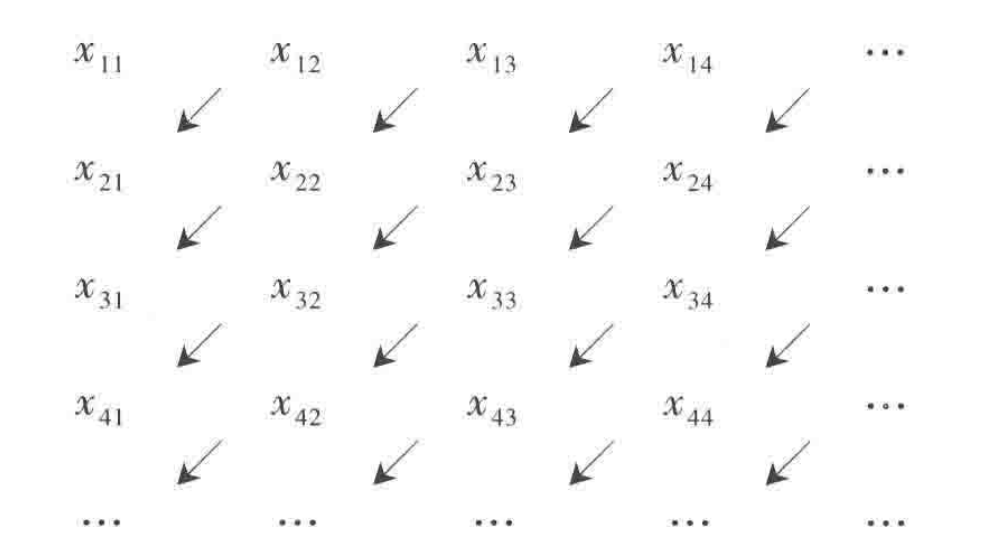
\includegraphics[width=0.7\linewidth]{figure/C1/8e9c0c930834b91d997911bb6ae34b5a}
	\end{center}
	

	把所有的元素排列成
	
	$$
	x_{11}, x_{12}, x_{21}, x_{13}, x_{22}, x_{31}, x_{14}, x_{23}, x_{32}, x_{41}, \cdots,
	$$
	这些集 $E_n$ 的任何两个如果有公共元素，那么这些公共元素将在上面的排列中不止出现一次.因此一切正整数的集里有一个子集 $T\subset\Z_+$ 使得 $S \sim T$ ，这就证明了 $S$ 是至多可数的.因为 $E_1 \subset S$ ，而 $E_1$ 是无限的，所以 $S$ 也是无限的，从而是可数的.
	
\end{proof}
\begin{corollary}\label{1.9.8}
	假定 $A$ 是至多可数的，并且对应于每个 $\alpha \in A$ 的 $B_\alpha$ 是至多可数
	的．令
	
	$$
	T=\bigcup_{\alpha \in A} B_\alpha
	$$
	
	
	那么 $T$ 是至多可数的．
\end{corollary}
$T$是\ref{uniofconset}中的$S$的一个子集.
\begin{proposition}
	\label{couofdes}
	$A_i$ 是可数集，$B_n=A_1 \times \cdots \times A_n$ 那么 $B_n$ 是可数的.
	
	换言之，可数集的有限次 Descartes 积是可数的
\end{proposition}

\begin{proof}
	$n=2$ 时 $ B_2=A_1 \times A_2=\left\{\left(x_1, x_2\right): x_1 \in A_1, x_2 \in A_2\right\}$
	
	令 $a_{i j}=\left(x_{1 i} , x_{2 j}\right)$ 由\ref{1.9.8}中的构造. $B_2$ 可数
	
	设 $B_{k-1}$ 可数
	
	$$
	B_k=A_1 \times \cdots A_{k-1} \times A_k=B_{k-1} \times A_k
	$$
	可数.
\end{proof}

\begin{remark}
	可数集的可数 次 Descartes 积不是可数的，使用下一节的定义，这个集合与 $\mathbb{R}$ 等势.
\end{remark}

下面我们考察一些集合的可数性.
\begin{proposition}
		$\Z,\Q$可数，$\R$不可数.
\end{proposition}

\begin{proof}
	对$\Z$ $f(n)=\left\{\begin{array}{cc}\dfrac{n}{2} & n \text { 是偶数 } \\ -\dfrac{n-1}{2} & n \text { 是奇数 }\end{array}\right.$
	
	对$\Q$由\ref{couofdes}可得
	
	对 $\mathbb{R}$ ,只需证 $(0,1)$ 内的所有实数不可数.
	
	如若不然，将所有 $(0,1)$ 内的实数用十进小数列出
	
	$$
	\begin{aligned}
		& r_1=0 . \overline{a_{11} a_{12} a_{13} a_{14}} \\
		& r_2=0 . \overline{a_{21} a_{22} a_{23} a_{24}} \cdots \\
		& r_3=0 . \overline{a_{31} a_{32} a_{33} a_{34}} \cdots \\
		& r_4=0 . \overline{a_{41} a_{42} a_{43} a_{44}} \cdots
	\end{aligned}
	$$
	
	
	构造 $b=0 . \overline{b_1 b_2 b_3 b_4} \cdots$ 使得 $b_1 \neq a_{11}, b_2 \neq a_{22}, b_3 \neq a_{33} \cdots$
	比如记 
	
	$\ b_n=\left[\begin{array}{ll}1 & \text { 若 }a_{n n} \neq 1 \\ 2 &\text { 若 } a_{n n}=1\end{array}\right.$
	
	$b$这个实数不在列表当中 ，矛盾，故不可数.
\end{proof}


\begin{lemma}(像-原像引理)
	设 \( f: X \to Y \) 是两个集合 \( X \) 和 \( Y \) 之间的映射，则以下命题成立：
	
	\begin{enumerate}
		\item[(0)]
		\begin{tabular}{ll}
			(a) & \( X = f^{-1}(Y) \) \\
			(b) & \( \varnothing  = f^{-1}(\varnothing ) \)
		\end{tabular}
		
		\item[(1)]
		\begin{tabular}{ll}
			(a) & 对于任意子集 \( U \subset X \)，有 \( U \subset f^{-1}(f(U)) \) \\
			(b) & 进一步，如果 \( f \) 是单射，则有 \( U = f^{-1}(f(U)) \)
		\end{tabular}
		
		\item[(2)]
		\begin{tabular}{ll}
			(a) & 对于任意子集 \( V \subset Y \)，有 \( V \supset f(f^{-1}(V)) \) \\
			(b) & 进一步，如果 \( f \) 是满射，则有 \( V = f(f^{-1}(V)) \)
		\end{tabular}
		
		\item[(3)] 对于 \( X \) 的任意一族子集 \(\{U_i\}_{i \in I}\)，有
		\[ f\left(\bigcup_{i \in I} U_i\right) = \bigcup_{i \in I} f(U_i) \]
		
		\item[(4)] 对于 \( X \) 的任意一族子集 \(\{U_i\}_{i \in I}\)，有
		\[ f\left(\bigcap_{i \in I} U_i\right) \subseteq \bigcap_{i \in I} f(U_i) \]
		
		\item[(5)]
		\begin{tabular}{ll}
			(a) & 对于任意子集 \( U \subset X \)，有 \( f(X \setminus U) \supset f(X) \setminus f(U) \) \\
			(b) & 进一步，如果 \( f^{-1}(f(U)) = U \)，则有 \( f(X \setminus U) = f(X) \setminus f(U) \)
		\end{tabular}
		
		\item[(6)] 对于 \( Y \) 的任意一族子集 \(\{V_i\}_{i \in I}\)，有
		\[ f^{-1}\left(\bigcup_{i \in I} V_i\right) = \bigcup_{i \in I} f^{-1}(V_i) \]
		
		\item[(7)] 对于 \( Y \) 的任意一族子集 \(\{V_i\}_{i \in I}\)，有
		\[ f^{-1}\left(\bigcap_{i \in I} V_i\right) = \bigcap_{i \in I} f^{-1}(V_i) \]
		
		\item[(8)] 对于任意子集 \( V \subset Y \)，有
		\[ f^{-1}(Y \setminus V) = X \setminus f^{-1}(V) \]
	\end{enumerate}
\end{lemma}

\begin{proof}
	\begin{enumerate}
		\item[(0)]
		\begin{enumerate}
			\item[(a)] 对于任意 \( x \in X \)，有 \( f(x) \in Y \)，因此 \( x \in f^{-1}(Y) \)，所以 \( X \subseteq f^{-1}(Y) \)。又因为 \( f^{-1}(Y) \subseteq X \)，所以 \( X = f^{-1}(Y) \)。
			
			\item[(b)] 因为 \( f^{-1}(\emptyset) = \{ x \in X \mid f(x) \in \emptyset \} = \emptyset \)，所以 \( \emptyset = f^{-1}(\emptyset) \)。 \end{enumerate}
		
		\item[(1)]
		\begin{enumerate}
			\item[(a)] 对于任意 \( x \in U \)，有 \( f(x) \in f(U) \)，因此 \( x \in f^{-1}(f(U)) \)，所以 \( U \subseteq f^{-1}(f(U)) \)。
			
			\item[(b)] 如果 \( f \) 是单射，且 \( x \in f^{-1}(f(U)) \)，则 \( f(x) \in f(U) \)，即存在 \( u \in U \) 使得 \( f(x) = f(u) \)。由于 \( f \) 是单射，所以 \( x = u \in U \)，因此 \( f^{-1}(f(U)) \subseteq U \)。结合 (1a) 可得 \( U = f^{-1}(f(U)) \)。 \end{enumerate}
		
		\item[(2)]
		\begin{enumerate}
			\item[(a)] 对于任意 \( y \in f(f^{-1}(V)) \)，存在 \( x \in f^{-1}(V) \) 使得 \( f(x) = y \)。根据定义，\( f(x) \in V \)，所以 \( y \in V \)，因此 \( f(f^{-1}(V)) \subseteq V \)。
			
			\item[(b)] 如果 \( f \) 是满射，对于任意 \( y \in V \)，存在 \( x \in X \) 使得 \( f(x) = y \)。因为 \( y \in V \)，所以 \( x \in f^{-1}(V) \)，因此 \( y \in f(f^{-1}(V)) \)，所以 \( V \subseteq f(f^{-1}(V)) \)。结合 (2a) 可得 \( V = f(f^{-1}(V)) \)。 \end{enumerate}
		
		\item[(3)] 对于任意 \( y \in f\left(\bigcup_{i \in I} U_i\right) \)，存在 \( x \in \bigcup_{i \in I} U_i \) 使得 \( f(x) = y \)。这意味着存在 \( i \in I \) 使得 \( x \in U_i \)，因此 \( y \in f(U_i) \)，所以 \( y \in \bigcup_{i \in I} f(U_i) \)。反之，对于任意 \( y \in \bigcup_{i \in I} f(U_i) \)，存在 \( i \in I \) 使得 \( y \in f(U_i) \)，因此存在 \( x \in U_i \) 使得 \( f(x) = y \)，所以 \( y \in f\left(\bigcup_{i \in I} U_i\right) \)。因此等式成立。
		
		\item[(4)] 对于任意 \( y \in f\left(\bigcap_{i \in I} U_i\right) \)，存在 \( x \in \bigcap_{i \in I} U_i \) 使得 \( f(x) = y \)。对于任意 \( i \in I \)，有 \( x \in U_i \)，因此 \( y \in f(U_i) \)，所以 \( y \in \bigcap_{i \in I} f(U_i) \)。
		
		\item[(5)]
		\begin{enumerate}
			\item[(a)] 对于任意 \( y \in f(X) \setminus f(U) \)，存在 \( x \in X \) 使得 \( f(x) = y \) 且 \( x \notin U \)，即 \( x \in X \setminus U \)，因此 \( y \in f(X \setminus U) \)。
			
			\item[(b)] 如果 \( f^{-1}(f(U)) = U \)，对于任意 \( y \in f(X) \setminus f(U) \)，假设 \( y \in f(U) \)，则存在 \( x \in U \) 使得 \( f(x) = y \)，这意味着 \( x \in f^{-1}(f(U)) = U \)，矛盾。因此 \( f(X \setminus U) \subseteq f(X) \setminus f(U) \)。结合 (5a) 可得 \( f(X \setminus U) = f(X) \setminus f(U) \)。 \end{enumerate}
		
		\item[(6)] 对于任意 \( x \in f^{-1}\left(\bigcup_{i \in I} V_i\right) \)，有 \( f(x) \in \bigcup_{i \in I} V_i \)，即存在 \( i \in I \) 使得 \( f(x) \in V_i \)，因此 \( x \in f^{-1}(V_i) \)，所以 \( x \in \bigcup_{i \in I} f^{-1}(V_i) \)。反之亦然，因此等式成立。
		
		\item[(7)] 对于任意 \( x \in f^{-1}\left(\bigcap_{i \in I} V_i\right) \)，对于任意 \( i \in I \)，有 \( f(x) \in V_i \)，因此 \( x \in f^{-1}(V_i) \)，所以 \( x \in \bigcap_{i \in I} f^{-1}(V_i) \)。反之亦然，因此等式成立。
		
		\item[(8)] 对于任意 \( x \in f^{-1}(Y \setminus V) \)，有 \( f(x) \in Y \setminus V \)，即 \( f(x) \notin V \)，因此 \( x \notin f^{-1}(V) \)，所以 \( x \in X \setminus f^{-1}(V) \)。反之亦然，因此等式成立。
	\end{enumerate}
\end{proof}
现在，我们用集合的方式，对映射再此定义，同时我们可以定义出二元运算的集合论形式.
\begin{definition}指派法则是两个集合的笛卡儿积 $C \times D$ 的一个子集 $r$，该子集满足这样的条件：$C$ 的每一个元素最多是 $r$ 中一个有序偶对的第一个坐标.
	
	这样，$C \times D$ 的一个子集 $r$ 如果满足
	
	$$
	\left[(c, d) \in r \text { 并且 }\left(c, d^{\prime}\right) \in r\right] \Longrightarrow\left[d=d^{\prime}\right] \text {, }
	$$
	则成为一个指派法则．我们可以将 $r$ 设想成一种指派方法，为 $C$ 的元素 $c$ 配置 $D$ 的满足 $(c, d) \in r$的元素 $d$ .
	
	对于一个指派法则 $r$ ，其定义域是由 $r$ 的元素的所有第一个坐标组成的 $C$ 的子集，其值域是由 $r$ 的元素的所有第二个坐标组成的 $D$ 的子集，即
	
	$r$ 的定义域 $=\{c $: 存在 $d \in D$ ，使得 $(c, d) \in r\}$ ，
	
	$r$ 的值域 $=\{d $ :存在 $c \in C$ ，使得 $(c, d) \in r\}$ ．
	
	函数$f$是指派法则$r$,与其定义域和值域三者组成的整体.
\end{definition}
\begin{definition}
	集合  $A $ 中的一个二元运算是将  $A \times A$ 映到  $A  $中的一个函数$  f $
\end{definition}
这样无论是整个实数的体系，还是函数的定义，或者是加减乘除的二元运算，都建立在公理化的集合论之上.
%
% 第10节：集合的势
% !TEX root = ../../../main.tex
% 所属：第一部分：单变量分析学 / 第1章：实数理论——从Peano公理到实数的连续性
% 节：1.10 集合的势
% 正文按原文件顺序保存；由 ../chapter1.tex 调用。
\section{集合的势}
\begin{definition}
	设 $A$, $B$ 是两个集合. 如果存在 $A$ 到 $B$ 的双射（即一一对应），则称 $A$ 与 $B$ \textbf{等势}，记作 $A \approx B$.
	
	集合的\textbf{势}（或基数）是集合在等势关系下的等价类，记作 $\operatorname{Card}(A)$ 或 $|A|$.
\end{definition}

容易验证 $\approx$ 是一个等价关系. 有限集的势就是其元素的个数；无限集的势则刻画了"无穷"的不同层次.

\begin{definition}
	设 $A$, $B$ 为集合. 若存在 $A$ 到 $B$ 的单射，则称 $A$ 的势\textbf{小于等于} $B$ 的势，记作 $\operatorname{Card}(A) \leqslant \operatorname{Card}(B)$.
	
	若 $\operatorname{Card}(A) \leqslant \operatorname{Card}(B)$ 且 $\operatorname{Card}(A) \neq \operatorname{Card}(B)$，则称 $A$ 的势\textbf{严格小于} $B$ 的势，记作 $\operatorname{Card}(A) < \operatorname{Card}(B)$.
\end{definition}

\begin{theorem}(Cantor--Bernstein 定理)
	若 $\operatorname{Card}(A) \leqslant \operatorname{Card}(B)$ 且 $\operatorname{Card}(B) \leqslant \operatorname{Card}(A)$，则 $\operatorname{Card}(A) = \operatorname{Card}(B)$.
\end{theorem}
这个证明我们在将来的拓扑学笔记中给出
\begin{definition}
	可数无穷集的势记作 $\aleph_0$（阿列夫零）. 即
	\[
	\aleph_0 := \operatorname{Card}(\N).
	\]
	势不超过 $\aleph_0$ 的集合称为\textbf{至多可数}的.
\end{definition}

由前几节的讨论，我们有
\[
\operatorname{Card}(\Z) = \operatorname{Card}(\Q) = \aleph_0.
\]
更一般地，可数个可数集的并仍是可数的.

\begin{definition}
	实数集 $\R$ 的势称为\textbf{连续统势}，记作 $\mathfrak{c}$（即 $2^{\aleph_0}$）.
	\[
	\mathfrak{c} := \operatorname{Card}(\R) = 2^{\aleph_0}.
	\]
\end{definition}

我们已经用对角线法证明了 $\R$ 不可数，因此 $\aleph_0 < \mathfrak{c}$.

\begin{theorem}[Cantor]
	对任意集合 $A$，有 $\operatorname{Card}(A) < \operatorname{Card}(\mathcal{P}(A))$，其中 $\mathcal{P}(A)$ 是 $A$ 的幂集. 特别地，
	\[
	\aleph_0 < 2^{\aleph_0} < 2^{2^{\aleph_0}} < \cdots,
	\]
	即存在无穷多个不同的无穷基数.
\end{theorem}

\textbf{注：}
	是否存在一个集合，其势严格介于 $\aleph_0$ 与 $\mathfrak{c}$ 之间？Cantor 猜测不存在这样的集合，即 $\mathfrak{c} = \aleph_1$（$\aleph_1$ 是大于 $\aleph_0$ 的最小基数）. 这一猜想称为\textbf{连续统假设}（Continuum Hypothesis, CH）.
	
	G\"{o}del (1940) 证明了 CH 与 ZFC 公理系统相容（不可证伪）；Cohen (1963) 证明了 CH 的否定也与 ZFC 相容（不可证明）. 因此，CH 独立于 ZFC —— 在标准的集合论公理下，它既不能被证明，也不能被否定.



	有限集的势显然小于 $\aleph_0$. 因此基数的无界递增链为
	\[
	0, 1, 2, \ldots, n, \ldots < \aleph_0 < 2^{\aleph_0} < 2^{2^{\aleph_0}} < \cdots.
	\]


%
% 第11节：复数域
% !TEX root = ../../../main.tex
% 所属：第一部分：单变量分析学 / 第1章：实数理论——从Peano公理到实数的连续性
% 节：1.11 复数域
% 正文按原文件顺序保存；由 ../chapter1.tex 调用。
\section{复数域}
\begin{definition}
	
	在 $ \mathbb{R} \times \mathbb{R}$  上定义如下等价关系 
	$$(a, b) \sim(c, d):=a=c \text { 且 } b=d$$
	$$\mathbb{C}:=\mathbb{R} \times \mathbb{R} / \sim$$
	
	
	设 $x=(a, b), y=(c, d)$ 是两个复数．我们定义：
	
	$$
	\begin{aligned}
		x+y & =(a+c, b+d) \\
		x y & =(a c-b d, a d+b c)
	\end{aligned}
	$$
	$(\C,+,\cdot)$是一个域，$(1,0)$视作$1$,$(0,0)$视作$0$
	$$\dfrac{1}{x}:=(\dfrac{a}{a^2+b^2},-\dfrac{b}{a^2+b^2})$$
	规定$(0,1)=i,(0,1)\cdot(0,1)=i^2=(-1,0)$
	
	习惯上，记$(a,b)=a+bi$
\end{definition}
\begin{definition}
	如果 $a, b$ 是实数，而 $z=a+b i$ ，就把复数 $\bar{z}=a-b i$ 叫做 $z$ 的共轭数.数 $a, b$ 分别叫做 $z$ 的实部和虚部.
	
	有时写成
	
	$$
	a=\operatorname{Re}(z), \quad b=\operatorname{Im}(z)
	$$
	
	
\end{definition}
\begin{proposition}
	\label{proofcon}
	如果 $z$ 及 $w$ 是复数，那么
	
	（a）$\overline{z+w}=\bar{z}+\bar{w}$ ，
	
	（b）$\overline{z w}=\bar{z} \cdot \bar{w}$ ，
	
	（c）$z+\bar{z}=2 \operatorname{Re}(z), \quad z- \bar{z}=2 i \operatorname{Im}(z)$ ．
	
	（d）$z \bar{z}$ 是实数且是正数（除了 $z=0$ 时）
\end{proposition}

\begin{proof}
	证（a），（b），（c）都十分明显，今证（d）．将 $z$ 写成 $z=a+b i$ ，并注意 $z \bar{z}= a^2+b^2$ .就行了.
\end{proof}
\begin{definition}
	如果 $z$ 是一复数，它的绝对值 $|z|$ 是 $z \bar{z}$ 的非负平方根；即 $|z|=(z \bar{z})^{1 / 2}$ .
	
\end{definition}

\begin{remark}
	当 $x$ 是实数时 $\bar{x}=x$ ，因此，$|x|=\sqrt{x^2}$ ．于是，如果 $x \geqslant 0,|x|=x$ ：如果 $x<0,|x|=-x$
\end{remark} 
\begin{proposition}
		设 $z$ 和 $w$ 都是复数，那么
	
	（a）$|z|>0$ 除非 $z=0,|0|=0$ ，
	
	（b）$|\bar{z}|=|z|$ ，
	
	（c）$|z w|=|z||w|$ ，
	
	（d）$|\operatorname{Re} z| \leqslant|z|$ ，
	
	（e）$|z+w| \leqslant|z|+|w|$ ．
\end{proposition}

\begin{proof}
	（a）及（b）是显然的．设 $z=a+b i, w=c+d i, a, b, c, d$ 为实数．
	
	于是
	
	$$
	\begin{aligned}
		|z w|^2 & =(a c-b d)^2+(a d+b c)^2 \\
		& =\left(a^2+b^2\right)\left(c^2+d^2\right)=|z|^2|w|^2
	\end{aligned}
	$$
	
	
	或 $|z w|^2=(|z||w|)^2$ .由定理$1.8.12$所说的惟一性，便能推得（c）.
	
	今证（d），注意 $a^2 \leqslant a^2+b^2$ ，由此，
	
	$$
	|a|=\sqrt{a^2} \leqslant \sqrt{a^2+b^2} .
	$$
	
	
	今证（e），注意 $\bar{z} w$ 是 $z \bar{w}$ 的共轭数，所以 $z \bar{w}+\bar{z} w=2 \operatorname{Re}(z \bar{w})$ .由此，
	
	$$
	\begin{aligned}
		|z+w|^2 & =(z+w)(\bar{z}+\bar{w})=\bar{z}+z \bar{w}+\bar{z} w+w \bar{w} \\
		& =|z|^2+2 \operatorname{Re}(z \bar{w})+|w|^2 \\
		& \leqslant|z|^2+2|z \bar{w}|+|w|^2 \\
		& =|z|^2+2|z||w|+|w|^2=(|z|+|w|)^2 .
	\end{aligned}
	$$
	
	
	两端开平方即得（e）.
\end{proof}
\begin{proposition}
	(Cauchy-Schawtz不等式)
	如果 $a_1, a_2, \cdots, a_n$ 及 $b_1, b_2, \cdots, b_n$ 都是复数，那么
	
	$$
	\left|\sum_{j=1}^n a_j \bar{b}_j\right|^2 \leqslant \sum_{j=1}^n\left|a_j\right|^2 \sum_{j=1}^n\left|b_j\right|^2 .
	$$
	\label{Cauchy-Schawtz不等式}
\end{proposition}

\begin{proof}
	设 $A=\Sigma\left|a_j\right|^2, B=\Sigma\left|b_j\right|^2, C=\Sigma a_j \bar{b}_j$（在本证明的所有和中，$j$ 遍历 $1, \cdots, n$ 诸值）.
	
	如果 $B=0$ ，那么 $b_1=\cdots=b_n=0$ ，而定理的结论是明显的.
	
	因此，可假定 $B>0$ ．由定理 \ref{proofcon}，有
	
	$$
	\begin{aligned}
		\sum\left|B a_j-C b_j\right|^2 & =\sum\left(B a_j-C b_j\right)\left(B \bar{a}_j-\bar{Cb_j}\right) \\
		& =B^2 \sum\left|a_j\right|^2-B \bar{C} \sum a_j \bar{b}_j-B C \sum \bar{a}_j b_j+|C|^2 \sum\left|b_j\right|^2 \\
		& =B^2 A-B|C|^2 \\
		& =B\left(A B-|C|^2\right) .
	\end{aligned}
	$$
	
	
	因第一个和中的每一项非负，而知
	
	$$
	B\left(A B-|C|^2\right) \geqslant 0 .
	$$
	
	
	由 $B>0$ 推得 $A B-|C|^2 \geqslant 0$ ．这就是要证的不等式．
\end{proof}
%
% 第12节：欧氏空间
% !TEX root = ../../../main.tex
% 所属：第一部分：单变量分析学 / 第1章：实数理论——从Peano公理到实数的连续性
% 节：1.12 欧氏空间
% 正文按原文件顺序保存；由 ../chapter1.tex 调用。
\section{欧氏空间}
\begin{definition}
	$\R^k$定义为k个$\R$的笛卡尔积.
	
	$\R^k=\left\{\boldsymbol{x}:\boldsymbol{x}=\left(x_1, x_2, \cdots, x_k\right),x_1,x_2,\cdots,x_k\in\R\right\}$
	
	称$\R^k$中的元素为向量，
	
	如果  $\boldsymbol{y}=\left(y_1, \cdots, y_k\right)$ 
	,而$\alpha\in\R$令
	
	$$
	\begin{aligned}
		\boldsymbol{x}+\boldsymbol{y} & =\left(x_1+y_1, x_2+y_2, \cdots, x_k+y_k\right), \\
		\alpha \boldsymbol{x} & =\left(\alpha x_1, \alpha x_2, \cdots, \alpha x_k\right)
	\end{aligned}
	$$
	
	
	于是 $\boldsymbol{x}+\boldsymbol{y}\in \R^k, \alpha \boldsymbol{x} \in \R^k$ .这就规定了向量的加法及向量的数乘.显然的，这两种运算满足交换律，结合律和分配律.而使 $\R^k$ 成为实数域上的向量空间. $\R^k$ 的零元是一切坐标都是 0 的点 $\mathbf{0}$ ．
\end{definition}
\begin{definition}
	$\boldsymbol{x}$ 与 $\boldsymbol{y}$ 的＂内积＂为
	
	$$
	\boldsymbol{x} \cdot \boldsymbol{y}=\sum_{i=1}^k x_i y_i
	$$
	
	
	又定义 $\boldsymbol{x}$ 的范数为
	
	$$
	|\boldsymbol{x}|=(\boldsymbol{x} \cdot \boldsymbol{x})^{1 / 2}=\left(\sum_{i=1}^k x_i^2\right)^{1 / 2} .
	$$
\end{definition}
具有上述的内积和范数的 $\R^k$ 称为 $k$ 维欧氏空间．
\begin{proposition}设 $\x, \y, \z \in \R^k, \lambda, \mu \in \R$
	\begin{enumerate}
		\item $\x\cdot\y=\y\cdot\x$
		\item $(\lambda\x+\mu\y)\cdot\z=\lambda\x\cdot\z+\mu\y\cdot\z$
		\item $(\x\cdot\y)^2\leqslant(\x\cdot\x)(\y\cdot\y)$
		
	\end{enumerate}
\end{proposition}
\begin{proof}
	1,2两条由内积的定义是显然的，3是\ref{Cauchy-Schawtz不等式}在实数下向量形式的表述，由\ref{Cauchy-Schawtz不等式}显然.
\end{proof}
\begin{proposition}设 $\x, \y, \z \in \R^k$ ，而 $\alpha$ 是实数．那么
	\begin{enumerate}
		\item$|\boldsymbol{x}| \geqslant 0$ 
		\item$|\boldsymbol{x}|=0$ 当且仅当; $\boldsymbol{x}=\mathbf{0}$ ；
		\item$|\alpha \boldsymbol{x}|=|\alpha||\boldsymbol{x}|$ ；
		\item$|\boldsymbol{x} \cdot \boldsymbol{y}| \leqslant|\boldsymbol{x}|| \boldsymbol{y} \mid$
		\item$|\boldsymbol{x}+\boldsymbol{y}| \leqslant|\boldsymbol{x}|+|\boldsymbol{y}|$
		\item$|\x-\z| \leqslant|\x-\y|+|\y-\z|$ ．
	\end{enumerate}
\end{proposition}
\begin{proof}
	1,2,3都显然成立．4是 Schwarz 不等式的直接结果,等价于1.12.3的第三条，由4
	$$
	\begin{aligned}
		|x+y|^2 & =(x+y) \cdot(x+y) \\
		& =x \cdot x+2 x \cdot y+y \cdot y \\
		& \leqslant|x|^2+2|x| y\left|+|y|^2\right. \\
		& =(|x|+|y|)^2
	\end{aligned}
	$$
	在5中用 $\x-\y$ 代 $\x$ ，用 $\y-\z$ 代 $\y$ 就得到5．
	
	
\end{proof}
%

%% ===== 第一部分：单变量分析学 / 第2章：一元实函数与基本初等函数——你所应当知晓的 =====
% !TEX root = ../../main.tex
\setchapterimage{figure/chapter2封面图.png}
\setchapterintro{这一章主要讲一些大学老师说的高中老师会讲，但高中老师说大学老师会讲的内容，内容不多，但在后续的计算，证明常常用到}
\chapter{一元实函数与基本初等函数——你所应当知晓的}



% 第1节：函数的性质
% !TEX root = ../../../main.tex
% 所属：第一部分：单变量分析学 / 第2章：一元实函数与基本初等函数——你所应当知晓的
% 节：2.1 函数的性质
% 正文按原文件顺序保存；由 ../chapter2.tex 调用。
\section{函数的性质}

\begin{definition}
	设 $f$ 定义在区间 $I \subset \R$ 上。
	\begin{enumerate}
		\item 若对任意 $x_1, x_2 \in I$ 且 $x_1 < x_2$，恒有 $f(x_1) \leqslant f(x_2)$，则称 $f$ 在 $I$ 上 {单调不减}（或{递增}）；
		\item 若对任意 $x_1, x_2 \in I$ 且 $x_1 < x_2$，恒有 $f(x_1) \geqslant f(x_2)$，则称 $f$ 在 $I$ 上 {单调不增}（或 {递减}）；
		\item 若对任意 $x_1, x_2 \in I$ 且 $x_1 < x_2$，恒有 $f(x_1) < f(x_2)$，则称 $f$ 在 $I$ 上 {严格单调递增}；
		\item 若对任意 $x_1, x_2 \in I$ 且 $x_1 < x_2$，恒有 $f(x_1) > f(x_2)$，则称 $f$ 在 $I$ 上 {严格单调递减}。
	\end{enumerate}
	以上四种情形统称为 $f$ 在 $I$ 上具有 {单调性}。
\end{definition}

\begin{proposition}
	若 $f$ 在区间 $I$ 上严格单调（递增或递减），则 $f$ 是 $I$ 到 $f(I)$ 的单射。特别地，$f: I \to f(I)$ 是双射，从而存在反函数 $f^{-1}: f(I) \to I$。
\end{proposition}

\begin{proof}
	不妨设 $f$ 严格递增。任取 $x_1, x_2 \in I$ 且 $x_1 \neq x_2$。若 $x_1 < x_2$，由严格递增性知 $f(x_1) < f(x_2)$；若 $x_1 > x_2$，则 $f(x_1) > f(x_2)$。无论哪种情形均有 $f(x_1) \neq f(x_2)$，故 $f$ 为单射。又 $f(I)$ 是 $f$ 的值域，故 $f: I \to f(I)$ 是满射，从而是双射，反函数存在。
\end{proof}

\begin{proposition}
	设 $f, g$ 均在区间 $I$ 上单调不减，则 $f + g$ 在 $I$ 上也单调不减。若 $f, g$ 均严格递增，则 $f + g$ 也严格递增。
\end{proposition}

\begin{proof}
	任取 $x_1, x_2 \in I$ 且 $x_1 < x_2$。由 $f, g$ 单调不减知
	\[
	f(x_1) \leqslant f(x_2), \quad g(x_1) \leqslant g(x_2).
	\]
	两式相加得 $(f+g)(x_1) = f(x_1) + g(x_1) \leqslant f(x_2) + g(x_2) = (f+g)(x_2)$，故 $f+g$ 单调不减。若均为严格递增，则不等号严格成立。
\end{proof}

\begin{proposition}
	设 $f$ 在区间 $I$ 上单调不减，$c \in \R$ 为常数。
	\begin{enumerate}
		\item 若 $c > 0$，则 $c f$ 在 $I$ 上单调不减；
		\item 若 $c < 0$，则 $c f$ 在 $I$ 上单调不增；
		\item 若 $c = 0$，则 $c f \equiv 0$ 既单调不减也单调不增。
	\end{enumerate}
	若 $f$ 严格递增，则 $c>0$ 时 $cf$ 严格递增，$c<0$ 时 $cf$ 严格递减。
\end{proposition}

\begin{proof}
	任取 $x_1, x_2 \in I$ 且 $x_1 < x_2$，则 $f(x_1) \leqslant f(x_2)$。
	当 $c > 0$ 时，$c f(x_1) \leqslant c f(x_2)$，故 $cf$ 单调不减；
	当 $c < 0$ 时，不等式反向得 $c f(x_1) \geqslant c f(x_2)$，故 $cf$ 单调不增；
	$c = 0$ 时显然。
\end{proof}

\begin{proposition}[复合函数的单调性]
	设 $f: I \to J$，$g: J \to \R$，其中 $I, J$ 为区间。
	\begin{enumerate}
		\item 若 $f$ 与 $g$ 同为递增或同为递减，则 $g \circ f$ 在 $I$ 上递增；
		\item 若 $f$ 与 $g$ 一个递增另一个递减，则 $g \circ f$ 在 $I$ 上递减。
	\end{enumerate}
\end{proposition}

\begin{proof}
	任取 $x_1, x_2 \in I$ 且 $x_1 < x_2$。
	\begin{enumerate}
		\item 若 $f, g$ 同为递增：$x_1 < x_2 \Rightarrow f(x_1) < f(x_2) \Rightarrow g(f(x_1)) < g(f(x_2))$；
		若同为递减：$x_1 < x_2 \Rightarrow f(x_1) > f(x_2) \Rightarrow g(f(x_1)) < g(f(x_2))$。故 $g \circ f$ 递增。
		\item 若 $f$ 递增而 $g$ 递减：$x_1 < x_2 \Rightarrow f(x_1) < f(x_2) \Rightarrow g(f(x_1)) > g(f(x_2))$；
		若 $f$ 递减而 $g$ 递增：$x_1 < x_2 \Rightarrow f(x_1) > f(x_2) \Rightarrow g(f(x_1)) > g(f(x_2))$。故 $g \circ f$ 递减。
	\end{enumerate}
\end{proof}

\begin{proposition}[反函数的单调性]
	设 $f$ 在区间 $I$ 上严格单调，则其反函数 $f^{-1}: f(I) \to I$ 存在，且 $f^{-1}$ 在 $f(I)$ 上具有与 $f$ 相同的单调性。
\end{proposition}

\begin{proof}
	不妨设 $f$ 严格递增。任取 $y_1, y_2 \in f(I)$ 且 $y_1 < y_2$。设 $x_1 = f^{-1}(y_1)$，$x_2 = f^{-1}(y_2)$，则 $f(x_1) = y_1$，$f(x_2) = y_2$。
	
	若 $x_1 \geqslant x_2$，由于 $f$ 严格递增，则 $y_1 = f(x_1) \geqslant f(x_2) = y_2$，与 $y_1 < y_2$ 矛盾。故 $x_1 < x_2$，即 $f^{-1}(y_1) < f^{-1}(y_2)$，所以 $f^{-1}$ 严格递增。
\end{proof}


\begin{definition}
	设 $f$ 定义在关于原点对称的集合 $D$ 上（即 $x \in D \Rightarrow -x \in D$）。
	\begin{enumerate}
		\item 若对任意 $x \in D$，恒有 $f(-x) = f(x)$，则称 $f$ 为 {偶函数}；
		\item 若对任意 $x \in D$，恒有 $f(-x) = -f(x)$，则称 $f$ 为 {奇函数}。
	\end{enumerate}
\end{definition}

	偶函数的图像关于 $y$ 轴对称；奇函数的图像关于原点中心对称。并非所有函数都是奇函数或偶函数，大多数函数既不是奇函数也不是偶函数。

\begin{proposition}[奇偶性的线性组合]
	设 $f, g$ 均为定义在关于原点对称的集合 $D$ 上的函数。
	\begin{enumerate}
		\item 若 $f, g$ 均为偶函数，则 $f + g$ 为偶函数；
		\item 若 $f, g$ 均为奇函数，则 $f + g$ 为奇函数；
		\item 若 $f$ 为偶（奇）函数，$c \in \R$，则 $cf$ 也为偶（奇）函数。
	\end{enumerate}
\end{proposition}

\begin{proof}
	\begin{enumerate}
		\item $(f+g)(-x) = f(-x) + g(-x) = f(x) + g(x) = (f+g)(x)$。
		\item $(f+g)(-x) = f(-x) + g(-x) = -f(x) - g(x) = -(f+g)(x)$。
		\item $(cf)(-x) = c \cdot f(-x) = c \cdot (\pm f(x)) = \pm (cf)(x)$。
	\end{enumerate}
\end{proof}

\begin{proposition}[奇偶性的乘积]
	设 $f, g$ 均为定义在关于原点对称的集合 $D$ 上的函数。
	\begin{enumerate}
		\item 若 $f, g$ 同为偶函数或同为奇函数，则 $f \cdot g$ 为偶函数；
		\item 若 $f$ 为偶函数而 $g$ 为奇函数，则 $f \cdot g$ 为奇函数。
	\end{enumerate}
\end{proposition}

\begin{proof}
	记 $h(x) = f(x) g(x)$。
	\begin{enumerate}
		\item 若 $f, g$ 同为偶函数：$h(-x) = f(-x)g(-x) = f(x)g(x) = h(x)$；
		若同为奇函数：$h(-x) = f(-x)g(-x) = (-f(x))(-g(x)) = f(x)g(x) = h(x)$。
		\item $h(-x) = f(-x)g(-x) = f(x) \cdot (-g(x)) = -f(x)g(x) = -h(x)$。
	\end{enumerate}
\end{proof}

\begin{proposition}[函数的奇偶分解]
	设 $f$ 定义在关于原点对称的集合 $D$ 上。则 $f$ 可以唯一地表示为一个偶函数与一个奇函数之和：
	\[
	f(x) = \frac{f(x) + f(-x)}{2} + \frac{f(x) - f(-x)}{2}.
	\]
	其中
	\[
	f_{\mathrm{even}}(x) := \frac{f(x) + f(-x)}{2}
	\]
	为偶函数，
	\[
	f_{\mathrm{odd}}(x) := \frac{f(x) - f(-x)}{2}
	\]
	为奇函数。
\end{proposition}

\begin{proof}
	先验证 $f_{\mathrm{even}}$ 为偶函数：
	\[
	f_{\mathrm{even}}(-x) = \frac{f(-x) + f(x)}{2} = f_{\mathrm{even}}(x).
	\]
	再验证 $f_{\mathrm{odd}}$ 为奇函数：
	\[
	f_{\mathrm{odd}}(-x) = \frac{f(-x) - f(x)}{2} = -\frac{f(x) - f(-x)}{2} = -f_{\mathrm{odd}}(x).
	\]
	显然 $f(x) = f_{\mathrm{even}}(x) + f_{\mathrm{odd}}(x)$。
	
	下证唯一性。假设另有偶函数 $g$ 与奇函数 $h$ 使得 $f = g + h$。则对任意 $x \in D$，
	\[
	\begin{aligned}
		f(x) &= g(x) + h(x), \\
		f(-x) &= g(-x) + h(-x) = g(x) - h(x).
	\end{aligned}
	\]
	两式相加得 $f(x) + f(-x) = 2g(x)$，故 $g(x) = \dfrac{f(x) + f(-x)}{2} = f_{\mathrm{even}}(x)$；
	两式相减得 $f(x) - f(-x) = 2h(x)$，故 $h(x) = \dfrac{f(x) - f(-x)}{2} = f_{\mathrm{odd}}(x)$。
	因此分解唯一。
\end{proof}

%
% 第2节：基本初等函数
% !TEX root = ../../../main.tex
% 所属：第一部分：单变量分析学 / 第2章：一元实函数与基本初等函数——你所应当知晓的
% 节：2.2 基本初等函数
% 正文按原文件顺序保存；由 ../chapter2.tex 调用。
\section{基本初等函数}
这一节介绍基本初等函数的一些常用的公式，它们可能是大学老师说的高中老师会讲，但高中老师说大学老师会讲的内容
\subsection*{代数恒等式}
\begin{proposition}[二项式定理]
	对任意 $n \in \N$，
	\[
	(x+y)^n = \sum_{k=0}^{n} \binom{n}{k} x^{n-k} y^k,
	\]
	其中 $\displaystyle\binom{n}{k} = \frac{n!}{k!(n-k)!}$ 为二项式系数。
\end{proposition}

\begin{proof}
	对 $n$ 用数学归纳法。$n=0$ 时 $(x+y)^0 = 1 = \binom{0}{0}x^0y^0$，成立。
	
	假设 $n$ 时成立，则
	\[
	\begin{aligned}
	(x+y)^{n+1} &= (x+y)(x+y)^n = (x+y)\sum_{k=0}^{n}\binom{n}{k}x^{n-k}y^k \\
	&= \sum_{k=0}^{n}\binom{n}{k}x^{n+1-k}y^k + \sum_{k=0}^{n}\binom{n}{k}x^{n-k}y^{k+1} \\
	&= x^{n+1} + \sum_{k=1}^{n}\left[\binom{n}{k}+\binom{n}{k-1}\right]x^{n+1-k}y^k + y^{n+1}.
	\end{aligned}
	\]
	由 Pascal 恒等式 $\binom{n}{k} + \binom{n}{k-1} = \binom{n+1}{k}$，即得 $n+1$ 时成立。
\end{proof}

\begin{proposition}[多项式定理]
	对任意 $n \in \N$，
	\[
	\left(\sum_{i=1}^{p} x_i\right)^n = \sum_{\substack{n_1+\cdots+n_p = n \\ n_1,\dots,n_p \in \N}} \binom{n}{n_1,\dots,n_p} \prod_{i=1}^{p} x_i^{n_i},
	\]
	其中 $\displaystyle\binom{n}{n_1,\dots,n_p} = \frac{n!}{n_1!\, n_2! \,\cdots\, n_p!}$ 为多项式系数。
\end{proposition}

\begin{proof}
	二项式定理的直接推广。展开乘积时，每一项对应从 $n$ 个因子中各选一个 $x_i$，$n_i$ 记录选取 $x_i$ 的次数。系数的组合意义即 $n$ 个元素中有 $n_i$ 个不可区分的第 $i$ 类元素时的排列数，由归纳法可严格证明。
\end{proof}

\begin{proposition}[平方差与 $n$ 次方差公式]
	对任意 $n \in \N$，$n \geqslant 1$，
	\[
	x^n - y^n = (x-y)(x^{n-1} + x^{n-2}y + \cdots + xy^{n-2} + y^{n-1}).
	\]
	当 $n$ 为奇数时，
	\[
	x^n + y^n = (x+y)(x^{n-1} - x^{n-2}y + \cdots - xy^{n-2} + y^{n-1}).
	\]
\end{proposition}

\begin{proof}
	对 $x^n - y^n$，将 $(x-y)$ 乘以右侧的几何级数和：
	\[
	\begin{aligned}
	(x-y)\sum_{k=0}^{n-1} x^{n-1-k}y^k &= \sum_{k=0}^{n-1} x^{n-k}y^k - \sum_{k=0}^{n-1} x^{n-1-k}y^{k+1} \\
	&= x^n + \sum_{k=1}^{n-1} x^{n-k}y^k - \sum_{k=0}^{n-2} x^{n-1-k}y^{k+1} - y^n = x^n - y^n.
	\end{aligned}
	\]
	当 $n$ 为奇数时，用 $-y$ 代入上式即得 $x^n + y^n = x^n - (-y)^n = (x+y)(\cdots)$。
\end{proof}

\begin{proposition}[前 $n$ 个正整数的方幂和]
	\[
	\sum_{k=1}^{n} k = \frac{n(n+1)}{2}, \qquad
	\sum_{k=1}^{n} k^2 = \frac{n(n+1)(2n+1)}{6}, \qquad
	\sum_{k=1}^{n} k^3 = \left[\frac{n(n+1)}{2}\right]^2.
	\]
\end{proposition}

\begin{proof}
	第一个公式：将 $S = 1+2+\cdots+n$ 倒序写为 $S = n+(n-1)+\cdots+1$，相加得 $2S = n(n+1)$。
	
	第二个公式：利用恒等式 $(k+1)^3 - k^3 = 3k^2 + 3k + 1$，对 $k=1$ 到 $n$ 求和：
	\[
	(n+1)^3 - 1 = 3\sum_{k=1}^{n} k^2 + 3\cdot\frac{n(n+1)}{2} + n,
	\]
	解得 $\sum k^2 = \dfrac{n(n+1)(2n+1)}{6}$。
	
	第三个公式：利用 $(k+1)^4 - k^4 = 4k^3 + 6k^2 + 4k + 1$ 求和，或注意到 $\sum k^3 = (\sum k)^2$，可由归纳法验证。
\end{proof}

\begin{proposition}[一元二次方程求根公式]
	方程 $ax^2 + bx + c = 0$（$a \neq 0$）的根为
	\[
	x_{1,2} = \frac{-b \pm \sqrt{b^2 - 4ac}}{2a}.
	\]
\end{proposition}

\begin{proof}
	配方：$a(x^2 + \frac{b}{a}x) + c = 0$，即 $a\left[(x+\frac{b}{2a})^2 - \frac{b^2}{4a^2}\right] + c = 0$，整理得 $(x+\frac{b}{2a})^2 = \frac{b^2-4ac}{4a^2}$，开方即得。
\end{proof}

\begin{proposition}[一元三次方程求根公式——Cardano 公式]
	考虑缺项三次方程
	\[
	t^3 + pt + q = 0,
	\]
	其中 $p, q \in \R$。令判别式 $\Delta = \left(\dfrac{q}{2}\right)^2 + \left(\dfrac{p}{3}\right)^3$。
	\begin{enumerate}
		\item 若 $\Delta > 0$，方程有一个实根和两个共轭复根：
		\[
		t_1 = u + v, \quad t_{2,3} = -\frac{u+v}{2} \pm i\frac{\sqrt{3}}{2}(u-v),
		\]
		其中 $u = \sqrt[3]{-\dfrac{q}{2} + \sqrt{\Delta}}$，$v = \sqrt[3]{-\dfrac{q}{2} - \sqrt{\Delta}}$。
		\item 若 $\Delta = 0$，三个实根（有重根）：
		\[
		t_1 = 2\sqrt[3]{-\frac{q}{2}}, \quad t_2 = t_3 = -\sqrt[3]{-\frac{q}{2}}.
		\]
		\item 若 $\Delta < 0$，三个互异实根（不可约情形），用三角形式表示：
		\[
		t_k = 2\sqrt{-\frac{p}{3}} \cos\left(\frac{1}{3}\arccos\left(\frac{-q/2}{\sqrt{-(p/3)^3}}\right) + \frac{2k\pi}{3}\right), \quad k = 0,1,2.
		\]
	\end{enumerate}
\end{proposition}

\begin{proof}
	设 $t = u + v$，则
	\[
	t^3 = (u+v)^3 = u^3 + v^3 + 3uv(u+v) = u^3 + v^3 + 3uv \cdot t.
	\]
	因此 $t^3 - 3uv \cdot t - (u^3+v^3) = 0$。与原方程 $t^3 + pt + q = 0$ 比较系数：
	\[
	uv = -\frac{p}{3}, \qquad u^3 + v^3 = -q.
	\]
	于是 $u^3$ 和 $v^3$ 是二次方程 $z^2 + qz - \left(\dfrac{p}{3}\right)^3 = 0$ 的两根，解得
	\[
	u^3, v^3 = -\frac{q}{2} \pm \sqrt{\left(\frac{q}{2}\right)^2 + \left(\frac{p}{3}\right)^3}.
	\]
	取 $u, v$ 满足 $uv = -p/3$（即 $uv$ 为实数），就得到 Cardano 公式。
	
	$\Delta < 0$ 时 $u, v$ 为共轭复数，用极坐标 $u = r e^{i\theta}$，$v = r e^{-i\theta}$，则 $t = u+v = 2r\cos\theta$，经计算得三角形式。
\end{proof}


	对一般三次方程 $ax^3 + bx^2 + cx + d = 0$（$a \neq 0$），先除以 $a$ 化为 $x^3 + Bx^2 + Cx + D = 0$，其中 $B = b/a$，$C = c/a$，$D = d/a$。作变量替换 $x = t - B/3$ 消去二次项，得
	\[
	t^3 + pt + q = 0, \qquad p = C - \frac{B^2}{3}, \quad q = \frac{2B^3}{27} - \frac{BC}{3} + D.
	\]
	求出 $t$ 后回代 $x = t - B/3$ 即得原方程的三根。



\subsection*{三角函数的基本公式}

我们假设读者已熟悉任意角弧度制下 $\sin x, \cos x, \tan x$ 等的几何定义以及诱导公式。以下 $x, y \in \R$，$n \in \N$。

\begin{proposition}[同角基本关系]
	\[
	\sin^2 x + \cos^2 x = 1, \quad
	1 + \tan^2 x = \sec^2 x, \quad
	1 + \cot^2 x = \csc^2 x.
	\]
	\[
	\tan x = \frac{\sin x}{\cos x}, \quad
	\cot x = \frac{\cos x}{\sin x}, \quad
	\sec x = \frac{1}{\cos x}, \quad
	\csc x = \frac{1}{\sin x}.
	\]
\end{proposition}

\begin{proof}
	在单位圆 $x^2+y^2=1$ 上，取角 $x$ 对应点 $(\cos x, \sin x)$，由定义直接得 $\sin^2 x + \cos^2 x = 1$。其余关系由定义出发，两边同除 $\cos^2 x$ 或 $\sin^2 x$ 即得。
\end{proof}

\begin{proposition}
	\[\begin{aligned}
		\sin(x \pm y) &= \sin x \cos y \pm \cos x \sin y, \\
		\cos(x \pm y) &= \cos x \cos y \mp \sin x \sin y, \\
		\tan(x \pm y) &= \frac{\tan x \pm \tan y}{1 \mp \tan x \tan y}.
	\end{aligned}\]
\end{proposition}
\begin{proof}
	用向量或几何方法证明余弦差公式。在单位圆上取点 $A(\cos x, \sin x)$，$B(\cos y, \sin y)$，如图所示：
	\begin{center}
	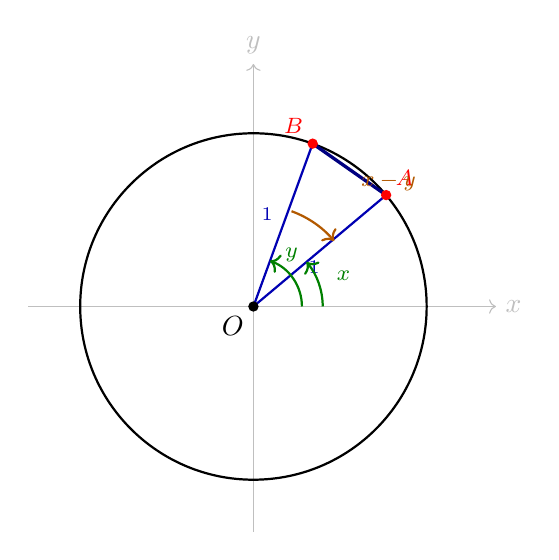
\begin{tikzpicture}[scale=2.2]
		% 坐标轴
		\draw[->, gray!50] (-1.3,0) -- (1.4,0) node[right] {$x$};
		\draw[->, gray!50] (0,-1.3) -- (0,1.4) node[above] {$y$};
		% 单位圆
		\draw[thick] (0,0) circle (1);
		% 点 A (角 x ~40°), B (角 y ~70°)
		\coordinate (A) at (0.766, 0.643);
		\coordinate (B) at (0.342, 0.940);
		% 半径 OA, OB
		\draw[thick, blue!70!black] (0,0) -- (A) node[midway, below, xshift=-2pt] {\scriptsize $1$};
		\draw[thick, blue!70!black] (0,0) -- (B) node[midway, left, yshift=4pt] {\scriptsize $1$};
		% 弦 AB
		\draw[very thick, blue!50!black] (A) -- (B);
		% 点
		\fill[red] (A) circle (0.03) node[above right, font=\footnotesize] {$A$};
		\fill[red] (B) circle (0.03) node[above left, font=\footnotesize] {$B$};
		% 原点
		\fill (0,0) circle (0.03) node[below left] {$O$};
		% 角 x (~40°)
		\draw[->, thick, green!50!black] (0.40,0) arc (0:40:0.40);
		\node[green!50!black, font=\footnotesize] at (0.52,0.18) {$x$};
		% 角 y (~70°)
		\draw[->, thick, green!50!black] (0.28,0) arc (0:70:0.28);
		\node[green!50!black, font=\footnotesize] at (0.22,0.30) {$y$};
		% 角 x-y
		\draw[->, thick, orange!70!black] (0.22,0.55) arc (70:40:0.58);
		\node[orange!70!black, font=\footnotesize] at (0.78,0.72) {$x-y$};
	\end{tikzpicture}
	\end{center}
	由两点间距离公式，
	\[
	\begin{aligned}
	|AB|^2 &= (\cos x - \cos y)^2 + (\sin x - \sin y)^2 = 2 - 2(\cos x \cos y + \sin x \sin y).
	\end{aligned}
	\]
	另一方面，在 $\triangle OAB$ 中由余弦定理（弦 $AB$ 所对的圆心角为 $|x-y|$）：
	\[
	|AB|^2 = |OA|^2 + |OB|^2 - 2|OA||OB|\cos(x-y) = 2 - 2\cos(x-y).
	\]

	比较得 $\cos(x-y) = \cos x \cos y + \sin x \sin y$。用 $-y$ 代 $y$ 得 $\cos(x+y)$。
	
	由诱导公式 $\sin(x+y) = \cos(\frac{\pi}{2}-x-y) = \cos((\frac{\pi}{2}-x)-y)$，展开余弦差公式即得正弦和公式。
	
	正切公式由 $\tan(x+y) = \dfrac{\sin(x+y)}{\cos(x+y)}$ 分子分母同除 $\cos x \cos y$ 得到。
\end{proof}

\begin{proposition}[倍角公式与半角公式]
	\[\begin{aligned}
		\sin 2x &= 2\sin x \cos x, \\
		\cos 2x &= \cos^2 x - \sin^2 x = 2\cos^2 x - 1 = 1 - 2\sin^2 x, \\
		\tan 2x &= \frac{2\tan x}{1 - \tan^2 x}.
	\end{aligned}\]
	\[
	\sin^2 \frac{x}{2} = \frac{1-\cos x}{2}, \qquad
	\cos^2 \frac{x}{2} = \frac{1+\cos x}{2}, \qquad
	\tan\frac{x}{2} = \frac{\sin x}{1+\cos x} = \frac{1-\cos x}{\sin x}.
	\]
\end{proposition}

\begin{proof}
	在和角公式中令 $y = x$ 即得倍角公式。由 $\cos 2x = 1 - 2\sin^2 x$ 解出 $\sin^2 x$，将 $x$ 换为 $x/2$ 即得半角正弦公式；由 $\cos 2x = 2\cos^2 x - 1$ 即得半角余弦公式。半角正切由 $\tan\dfrac{x}{2} = \dfrac{\sin(x/2)}{\cos(x/2)}$ 并利用半角公式化简得到。
\end{proof}

\begin{proposition}[三倍角公式]
	\[
	\sin 3x = 3\sin x - 4\sin^3 x, \qquad
	\cos 3x = 4\cos^3 x - 3\cos x.
	\]
\end{proposition}

\begin{proof}
	$\sin 3x = \sin(2x+x) = \sin 2x \cos x + \cos 2x \sin x = 2\sin x \cos^2 x + (1-2\sin^2 x)\sin x = 2\sin x(1-\sin^2 x) + \sin x - 2\sin^3 x = 3\sin x - 4\sin^3 x$。余弦公式同理，或由 $\cos 3x = \cos(2x+x)$ 展开。
\end{proof}

\begin{proposition}[积化和差与和差化积]
	积化和差：
	\[\begin{aligned}
		\sin x \cos y &= \tfrac{1}{2}[\sin(x+y) + \sin(x-y)], \\
		\cos x \sin y &= \tfrac{1}{2}[\sin(x+y) - \sin(x-y)], \\
		\cos x \cos y &= \tfrac{1}{2}[\cos(x+y) + \cos(x-y)], \\
		\sin x \sin y &= \tfrac{1}{2}[\cos(x-y) - \cos(x+y)].
	\end{aligned}\]
	
	和差化积：
	\[\begin{aligned}
		\sin x + \sin y &= 2\sin\tfrac{x+y}{2}\cos\tfrac{x-y}{2}, \\
		\sin x - \sin y &= 2\cos\tfrac{x+y}{2}\sin\tfrac{x-y}{2}, \\
		\cos x + \cos y &= 2\cos\tfrac{x+y}{2}\cos\tfrac{x-y}{2}, \\
		\cos x - \cos y &= -2\sin\tfrac{x+y}{2}\sin\tfrac{x-y}{2}.
	\end{aligned}\]
	
\end{proposition}

\begin{proof}
	积化和差：由两角和与差的正弦/余弦公式相加或相减即得。例如
	\[
	\sin(x+y) + \sin(x-y) = (\sin x \cos y + \cos x \sin y) + (\sin x \cos y - \cos x \sin y) = 2\sin x \cos y.
	\]
	和差化积：在积化和差公式中令 $u = \frac{x+y}{2}$，$v = \frac{x-y}{2}$，则 $x = u+v$，$y = u-v$，代入即得。
\end{proof}


\begin{proposition}[万能公式]
	令 $t = \tan\dfrac{x}{2}$，则
	\[
	\sin x = \frac{2t}{1+t^2}, \qquad
	\cos x = \frac{1-t^2}{1+t^2}, \qquad
	\tan x = \frac{2t}{1-t^2}.
	\]
\end{proposition}

\begin{proof}
	由半角公式：$\sin x = 2\sin\frac{x}{2}\cos\frac{x}{2}$，分子分母同除 $\cos^2\frac{x}{2}$ 得 $\sin x = \frac{2\tan(x/2)}{1+\tan^2(x/2)} = \frac{2t}{1+t^2}$。类似可得余弦和正切。
\end{proof}

\subsection*{反三角函数}

\begin{definition}
	$\arcsin: [-1,1] \to [-\frac{\pi}{2}, \frac{\pi}{2}]$，$\arccos: [-1,1] \to [0,\pi]$，$\arctan: \R \to (-\frac{\pi}{2}, \frac{\pi}{2})$ 分别为 $\sin, \cos, \tan$ 在各自限制区间上的反函数。
\end{definition}

\begin{proposition}[基本恒等式]
	对定义域内的 $x$，
	\[
	\sin\arcsin x = x, \quad \cos\arccos x = x, \quad \tan\arctan x = x.
	\]
	\[
	\arcsin(-x) = -\arcsin x, \quad \arccos(-x) = \pi - \arccos x, \quad \arctan(-x) = -\arctan x.
	\]
	\[
	\arcsin x + \arccos x = \frac{\pi}{2}, \qquad \arctan x + \operatorname{arccot} x = \frac{\pi}{2}.
	\]
\end{proposition}

\begin{proof}
	第一行由反函数定义直接得到。奇偶性：$\sin(-\arcsin x) = -\sin\arcsin x = -x$，且 $-\arcsin x \in [-\frac{\pi}{2},\frac{\pi}{2}]$，故 $\arcsin(-x) = -\arcsin x$。类似可证 $\arctan$。对 $\arccos$，$\cos(\pi - \arccos x) = -\cos\arccos x = -x$，且 $\pi - \arccos x \in [0,\pi]$，故 $\arccos(-x) = \pi - \arccos x$。
	
	互余关系：令 $\alpha = \arcsin x$，则 $\sin\alpha = x$，$\cos(\frac{\pi}{2}-\alpha) = \sin\alpha = x$，且 $\frac{\pi}{2}-\alpha \in [0,\pi]$，故 $\arccos x = \frac{\pi}{2}-\alpha = \frac{\pi}{2} - \arcsin x$。
\end{proof}

\begin{proposition}[反三角函数的三角值]
	\[
	\begin{aligned}
		\sin\arccos x &= \sqrt{1-x^2}, & \cos\arcsin x &= \sqrt{1-x^2}, \\
		\sin\arctan x &= \frac{x}{\sqrt{1+x^2}}, & \cos\arctan x &= \frac{1}{\sqrt{1+x^2}}, \\
		\tan\arcsin x &= \frac{x}{\sqrt{1-x^2}}, & \tan\arccos x &= \frac{\sqrt{1-x^2}}{x}.
	\end{aligned}
	\]
\end{proposition}

\begin{proof}
	以 $\sin\arccos x$ 为例：令 $\alpha = \arccos x \in [0,\pi]$，则 $\cos\alpha = x$，$\sin\alpha = \sqrt{1-\cos^2\alpha} = \sqrt{1-x^2}$（因 $\alpha \in [0,\pi]$ 时 $\sin\alpha \geqslant 0$）。其余类似，注意各反三角函数值域中三角函数的符号即可。
\end{proof}

\begin{proposition}[$\arctan$ 加法公式]
	\[
	\arctan x + \arctan y = \arctan\frac{x+y}{1-xy} \quad (xy < 1).
	\]
	当 $x > 0$，$xy > 1$ 时，等式右端加 $\pi$；当 $x < 0$，$xy > 1$ 时，右端减 $\pi$。
\end{proposition}

\begin{proof}
	令 $\alpha = \arctan x$，$\beta = \arctan y$，则 $\tan\alpha = x$，$\tan\beta = y$。由正切和角公式：
	\[
	\tan(\alpha+\beta) = \frac{\tan\alpha + \tan\beta}{1 - \tan\alpha\tan\beta} = \frac{x+y}{1-xy}.
	\]
	因此 $\alpha+\beta$ 是正切值为 $\frac{x+y}{1-xy}$ 的一个角，但 $\arctan$ 的值域为 $(-\frac{\pi}{2}, \frac{\pi}{2})$，需根据 $x, y$ 的符号和 $xy$ 与 $1$ 的大小关系调整分支。当 $xy<1$ 时 $|\alpha+\beta| < \frac{\pi}{2}$，等式直接成立；其余情形通过加减 $\pi$ 调整到正确象限。
\end{proof}


\subsection*{指数函数与对数函数}



\begin{proposition}[指数与对数的基本运算法则]
	对 $a>0$，$a \neq 1$，$x, y \in \R$，
	\[
	a^{x+y} = a^x a^y, \qquad (a^x)^y = a^{xy}, \qquad a^{-x} = \frac{1}{a^x}.
	\]
	对 $M, N > 0$，
	\[
	\log_a(MN) = \log_a M + \log_a N, \quad
	\log_a\frac{M}{N} = \log_a M - \log_a N, \quad
	\log_a M^p = p \log_a M.
	\]
\end{proposition}

\begin{proof}
	指数运算法则由有理指数的定义和确界延拓保证。对数运算法则是指数法则的逆命题：令 $u = \log_a M$，$v = \log_a N$，则 $M = a^u$，$N = a^v$，故 $MN = a^{u+v}$，从而 $\log_a(MN) = u+v = \log_a M + \log_a N$。其余同理。
\end{proof}

\begin{proposition}[换底公式]
	\[
	\log_a b = \frac{\log_c b}{\log_c a} \quad (c>0, c \neq 1).
	\]
\end{proposition}

\begin{proof}
	令 $y = \log_a b$，则 $a^y = b$。两边取以 $c$ 为底的对数得 $y \log_c a = \log_c b$，故 $y = \frac{\log_c b}{\log_c a}$。
\end{proof}



\subsection*{双曲函数}

\begin{definition}
	双曲正弦、双曲余弦和双曲正切分别定义为
	\[
	\sinh x = \frac{e^x - e^{-x}}{2}, \qquad
	\cosh x = \frac{e^x + e^{-x}}{2}, \qquad
	\tanh x = \frac{\sinh x}{\cosh x} = \frac{e^x - e^{-x}}{e^x + e^{-x}}.
	\]
	其余双曲函数定义为倒数：$\operatorname{csch} x = \dfrac{1}{\sinh x}$，$\operatorname{sech} x = \dfrac{1}{\cosh x}$，$\operatorname{coth} x = \dfrac{1}{\tanh x}$。
\end{definition}
\textbf{注}：双曲函数与三角函数有深刻的类比关系，许多三角恒等式在双曲情形下有几乎完全相同的形式（仅符号略有变化），这源于 Euler 公式 $e^{ix} = \cos x + i\sin x$ 以及 $\sinh x = -i\sin(ix)$，$\cosh x = \cos(ix)$。


\begin{proposition}[基本恒等式]
	\[
	\cosh^2 x - \sinh^2 x = 1, \qquad
	1 - \tanh^2 x = \operatorname{sech}^2 x.
	\]
\end{proposition}

\begin{proof}
	直接计算：
	\[
	\cosh^2 x - \sinh^2 x = \frac{(e^x+e^{-x})^2}{4} - \frac{(e^x-e^{-x})^2}{4} = \frac{4}{4} = 1.
	\]
	第二式由第一式两边同除 $\cosh^2 x$ 得到。
\end{proof}

\begin{proposition}[和差公式与倍角公式]
	\begin{align*}
		\sinh(x \pm y) &= \sinh x \cosh y \pm \cosh x \sinh y, \\
		\cosh(x \pm y) &= \cosh x \cosh y \pm \sinh x \sinh y.
	\end{align*}
	\[
	\sinh 2x = 2\sinh x \cosh x, \qquad
	\cosh 2x = \cosh^2 x + \sinh^2 x = 2\cosh^2 x - 1 = 1 + 2\sinh^2 x.
	\]
\end{proposition}

\begin{proof}
	以 $\sinh(x+y)$ 为例：
	\[
	\begin{aligned}
	\sinh x \cosh y + \cosh x \sinh y
	&= \frac{e^x-e^{-x}}{2} \cdot \frac{e^y+e^{-y}}{2} + \frac{e^x+e^{-x}}{2} \cdot \frac{e^y-e^{-y}}{2} \\
	&= \frac{e^{x+y} + e^{x-y} - e^{-x+y} - e^{-x-y}}{4} + \frac{e^{x+y} - e^{x-y} + e^{-x+y} - e^{-x-y}}{4} \\
	&= \frac{2e^{x+y} - 2e^{-(x+y)}}{4} = \frac{e^{x+y} - e^{-(x+y)}}{2} = \sinh(x+y).
	\end{aligned}
	\]
	其余公式类似可证。倍角公式在和差公式中令 $y = x$ 即得。
\end{proof}

\begin{proposition}[反双曲函数的对数表示]
	\[
	\begin{aligned}
		\sinh^{-1} x &= \ln\!\bigl(x + \sqrt{x^2+1}\bigr), \quad &x &\in \R, \\
		\cosh^{-1} x &= \ln\!\bigl(x + \sqrt{x^2-1}\bigr), \quad &x &\geqslant 1, \\
		\tanh^{-1} x &= \frac{1}{2}\ln\frac{1+x}{1-x}, \quad &|x| &< 1.
	\end{aligned}
	\]
\end{proposition}

\begin{proof}
	以 $\sinh^{-1} x$ 为例。令 $y = \sinh^{-1} x$，则 $x = \sinh y = \frac{e^y - e^{-y}}{2}$。乘以 $2e^y$ 得 $2x e^y = e^{2y} - 1$，即 $(e^y)^2 - 2x e^y - 1 = 0$。解关于 $e^y$ 的二次方程得 $e^y = x + \sqrt{x^2+1}$（取正根，因 $e^y > 0$），故 $y = \ln(x + \sqrt{x^2+1})$。
	
	$\cosh^{-1}x$ 同理：由 $x = \frac{e^y+e^{-y}}{2}$ 得 $e^y = x \pm \sqrt{x^2-1}$，因 $y \geqslant 0$ 时 $e^y \geqslant 1$，取正号得 $e^y = x + \sqrt{x^2-1}$。
	
	$\tanh^{-1} x$：由 $x = \frac{e^y-e^{-y}}{e^y+e^{-y}}$，令 $u = e^{2y}$，解得 $u = \frac{1+x}{1-x}$，故 $y = \frac{1}{2}\ln\frac{1+x}{1-x}$。
\end{proof}


%
% 第3节：常用不等式
% !TEX root = ../../../main.tex
% 所属：第一部分：单变量分析学 / 第2章：一元实函数与基本初等函数——你所应当知晓的
% 节：2.3 常用不等式
% 正文按原文件顺序保存；由 ../chapter2.tex 调用。
\section{常用不等式}

本节收集一元实分析中若干基本的不等式，它们将在后续章节中多次出现。

\begin{proposition}(Bernoulli 不等式)
	设 $x \geqslant -1$，$x \in \R$。
	\begin{enumerate}
		\item 若 $n \in \N$，则 $(1+x)^n \geqslant 1 + nx$；
		\item 若 $n$ 为偶数，则上式对任意实数 $x$ 成立。
	\end{enumerate}
	等号成立当且仅当 $n = 0,1$ 或 $x = 0$。
\end{proposition}

\begin{proof}
	对 $n$ 用数学归纳法。$n=0$ 时 $(1+x)^0 = 1 = 1+0\cdot x$；$n=1$ 时 $(1+x)^1 = 1+x$，等号均成立。
	
	假设 $n=k$ 时 $(1+x)^k \geqslant 1+kx$ 成立。则
	\[
	\begin{aligned}
	(1+x)^{k+1} &= (1+x)^k(1+x) \geqslant (1+kx)(1+x) \\
	&= 1 + (k+1)x + kx^2 \geqslant 1 + (k+1)x,
	\end{aligned}
	\]
	其中第一步用到 $1+x \geqslant 0$（因 $x \geqslant -1$）。等号成立当且仅当 $k=0$ 或 $x=0$，即 $n=0,1$ 或 $x=0$。
\end{proof}



\begin{proposition}(AM--GM) 不等式
	设 $a_1, a_2, \dots, a_n \geqslant 0$（$n \geqslant 2$），则
	\[
	\frac{a_1 + a_2 + \cdots + a_n}{n} \geqslant \sqrt[n]{a_1 a_2 \cdots a_n},
	\]
	等号成立当且仅当 $a_1 = a_2 = \cdots = a_n$。
\end{proposition}

以下给出两种证明。

\medskip
\noindent\textbf{证法一（数学归纳法）.}

\begin{proof}
	$n=2$ 时，由 $(\sqrt{a_1} - \sqrt{a_2})^2 \geqslant 0$ 得 $a_1 + a_2 \geqslant 2\sqrt{a_1a_2}$，成立。
	
	假设 $n=k$ 时成立。对 $n=k+1$，令
	\[
	A_k = \frac{a_1 + \cdots + a_k}{k}, \quad A_{k+1} = \frac{a_1 + \cdots + a_{k+1}}{k+1}.
	\]
	则 $a_1 + \cdots + a_k = kA_k$。由归纳假设，
	\[
	A_k \geqslant \sqrt[k]{a_1 \cdots a_k}.
	\]
	现在
	\[
	\begin{aligned}
	A_{k+1} &= \frac{kA_k + a_{k+1}}{k+1}
	= \frac{k}{k+1}A_k + \frac{1}{k+1}a_{k+1}.
	\end{aligned}
	\]
	如果 $a_{k+1} \geqslant A_k$，则 $A_{k+1} \geqslant A_k$；否则 $A_{k+1} < A_k$。用 $n=2$ 时的 AM--GM 于 $A_k$ 和 $a_{k+1}$：
	\[
	\frac{kA_k + a_{k+1}}{k+1} = \frac{k}{k+1}A_k + \frac{1}{k+1}a_{k+1}
	\geqslant A_k^{\frac{k}{k+1}} a_{k+1}^{\frac{1}{k+1}}.
	\]
	再结合 $A_k \geqslant \sqrt[k]{a_1\cdots a_k}$，有
	\[
	A_k^{\frac{k}{k+1}} a_{k+1}^{\frac{1}{k+1}}
	\geqslant (a_1\cdots a_k)^{\frac{1}{k+1}} a_{k+1}^{\frac{1}{k+1}}
	= (a_1\cdots a_k a_{k+1})^{\frac{1}{k+1}}.
	\]
	故 $A_{k+1} \geqslant \sqrt[k+1]{a_1\cdots a_{k+1}}$。等号条件由各步等号取法推得。
\end{proof}

\medskip
\noindent\textbf{证法二（向前--向后归纳法，Cauchy 方法）.}

\begin{proof}
	\textbf{第一步（向前）：} 先证 $n=2$ 成立，再由 $n=2^k$ 推出 $n=2^{k+1}$。
	
	$n=2$ 平凡。假设 $n=2^k$ 时成立。对 $2^{k+1}=2\cdot 2^k$ 个数 $a_1,\dots,a_{2^{k+1}}$：
	\[
	\frac{a_1+\cdots+a_{2^{k+1}}}{2^{k+1}}
	= \frac{1}{2}\left(\frac{a_1+\cdots+a_{2^k}}{2^k} + \frac{a_{2^k+1}+\cdots+a_{2^{k+1}}}{2^k}\right).
	\]
	由 $n=2$ 情形，上式
	\[
	\geqslant \sqrt{\frac{a_1+\cdots+a_{2^k}}{2^k} \cdot \frac{a_{2^k+1}+\cdots+a_{2^{k+1}}}{2^k}}.
	\]
	再由归纳假设，上式
	\[
	\geqslant \sqrt{\sqrt[2^k]{a_1\cdots a_{2^k}} \cdot \sqrt[2^k]{a_{2^k+1}\cdots a_{2^{k+1}}}}
	= \sqrt[2^{k+1}]{a_1\cdots a_{2^{k+1}}}.
	\]
	于是 AM--GM 对一切 $n=2^k$（$k \in \N$）成立。
	
	\textbf{第二步（向后）：} 假设不等式对 $n+1$ 成立，证对 $n$ 也成立。
	
	对任意 $n$ 个正数 $a_1,\dots,a_n$，令 $a_{n+1} = \frac{a_1+\cdots+a_n}{n}$。对 $n+1$ 个数用 AM--GM：
	\[
	\frac{a_1+\cdots+a_n + a_{n+1}}{n+1}
	\geqslant \sqrt[n+1]{a_1\cdots a_n \cdot a_{n+1}}.
	\]
	左边 $= \frac{n a_{n+1} + a_{n+1}}{n+1} = a_{n+1}$，故
	\[
	a_{n+1} \geqslant \sqrt[n+1]{a_1\cdots a_n \cdot a_{n+1}}.
	\]
	两边取 $n+1$ 次方，得 $a_{n+1}^{n+1} \geqslant a_1\cdots a_n \cdot a_{n+1}$，即 $a_{n+1}^n \geqslant a_1\cdots a_n$，从而
	\[
	\frac{a_1+\cdots+a_n}{n} = a_{n+1} \geqslant \sqrt[n]{a_1\cdots a_n}.
	\]
	向后步骤完成。由于对任意 $n$，可取 $m$ 使 $n \leqslant 2^m$，向前步骤给出 $2^m$ 时成立，向后步骤逐步降回到 $n$ 时成立。
	
	等号成立当且仅当所有 $a_i$ 相等，由各步等号条件追踪可得。
\end{proof}



\begin{proposition}[GM--HM 不等式]
	设 $a_1, a_2, \dots, a_n > 0$，则
	\[
	\sqrt[n]{a_1 a_2 \cdots a_n} \geqslant \frac{n}{\frac{1}{a_1} + \frac{1}{a_2} + \cdots + \frac{1}{a_n}},
	\]
	即几何平均不小于调和平均。等号成立当且仅当 $a_1 = a_2 = \cdots = a_n$。
\end{proposition}

\begin{proof}
	对正数 $\dfrac{1}{a_1}, \dfrac{1}{a_2}, \dots, \dfrac{1}{a_n}$ 应用 AM--GM 不等式：
	\[
	\frac{\frac{1}{a_1} + \frac{1}{a_2} + \cdots + \frac{1}{a_n}}{n}
	\geqslant \sqrt[n]{\frac{1}{a_1} \cdot \frac{1}{a_2} \cdots \frac{1}{a_n}}
	= \frac{1}{\sqrt[n]{a_1 a_2 \cdots a_n}}.
	\]
	两边取倒数即得 GM--HM 不等式。等号条件继承 AM--GM 的等号条件。
\end{proof}

\noindent 结合 AM--GM 和 GM--HM，得经典的均值不等式链：
\[
\frac{n}{\sum \frac{1}{a_i}} \;\leqslant\; \sqrt[n]{a_1\cdots a_n} \;\leqslant\; \frac{\sum a_i}{n},
\]
即调和平均 $\leqslant$ 几何平均 $\leqslant$ 算术平均。


\begin{proposition}(Cauchy--Schwarz 不等式)
	设 $a_1,\dots,a_n, b_1,\dots,b_n \in \R$，则
	\[
	\left(\sum_{i=1}^{n} a_i b_i\right)^2 \leqslant \left(\sum_{i=1}^{n} a_i^2\right)\left(\sum_{i=1}^{n} b_i^2\right).
	\]
	等号成立当且仅当存在常数 $\lambda \in \R$，使得 $a_i = \lambda b_i$（$i=1,\dots,n$）或所有 $b_i = 0$。
\end{proposition}

\begin{proof}[证法一（二次型判别法）]
	考虑关于 $t \in \R$ 的二次函数
	\[
	f(t) = \sum_{i=1}^{n} (a_i t + b_i)^2 = \left(\sum_{i=1}^{n} a_i^2\right) t^2 + 2\left(\sum_{i=1}^{n} a_i b_i\right) t + \left(\sum_{i=1}^{n} b_i^2\right).
	\]
	由于 $f(t)$ 为平方和，$f(t) \geqslant 0$ 对所有 $t \in \R$ 成立。故其判别式 $\Delta \leqslant 0$：
	\[
	\Delta = 4\left(\sum_{i=1}^{n} a_i b_i\right)^2 - 4\left(\sum_{i=1}^{n} a_i^2\right)\left(\sum_{i=1}^{n} b_i^2\right) \leqslant 0,
	\]
	整理即得 Cauchy 不等式。等号成立当且仅当 $f(t)=0$ 有重根，即存在 $t_0$ 使 $a_i t_0 + b_i = 0$ 对所有 $i$ 成立，也就是 $a_i$ 与 $b_i$ 成比例。
\end{proof}

\begin{proof}[证法二（Lagrange 恒等式法）]
	直接验证以下代数恒等式：
	\[
	\left(\sum_{i=1}^{n} a_i^2\right)\left(\sum_{i=1}^{n} b_i^2\right) - \left(\sum_{i=1}^{n} a_i b_i\right)^2
	= \frac{1}{2}\sum_{i=1}^{n}\sum_{j=1}^{n} (a_i b_j - a_j b_i)^2.
	\]
	右边非负，故左边非负，即得 Cauchy 不等式。等号成立当且仅当对所有 $i,j$ 有 $a_i b_j = a_j b_i$，即 $(a_1,\dots,a_n)$ 与 $(b_1,\dots,b_n)$ 成比例。
\end{proof}

\textbf{注：}
利用 Cauchy 不等式可导出许多有用的推论，例如：
	\[
	(a_1+\cdots+a_n)\left(\frac{1}{a_1}+\cdots+\frac{1}{a_n}\right) \geqslant n^2 \quad (a_i > 0).
	\]
	只需在 Cauchy 不等式中取 $b_i = 1/a_i$ 即可。


%

%% ===== 第一部分：单变量分析学 / 第3章：实数的八大基本定理 =====
% !TEX root = ../../main.tex
\setchapterimage{figure/chapter3封面图.png}
\setchapterintro{除了上一章已经讨论过的确界原理与Dedekind定理以外，这一章的讨论重点是剩余的实数基本定理，这一章分为两个部分，基础拓扑与数列，拓扑学部分的一些结论可以迁移到将来的多元函数部分中。这一章的一个问题就是前后的割裂，即使有八大定理的互证作为连接的桥梁，其练习还是有些牵强，我想这也就是为什么一般来说数分中的拓扑学会只涉及直线上与空间中的拓扑。本章的拓扑学部分参考Sydney的Topology without Tears}
\chapter{实数的八大基本定理}
本章我们来考量实数的八大基本定理.

\textbf{定理}：以下8条叙述等价.

\begin{enumerate}
	\item (确界原理)非空有上（下）界数集，必有上（下）确界
	\item （Dedekind 准则）设序对 $(A, A^{\prime})$ 为 $\R$ 的一个分划，则$A$无最大元， $A^{\prime}$ 有最小元．
	\item （单调有界原理）任何单调有界数列必有极限．
	\item （Cantor 区间套定理）若 $\left\{\left[a_n, b_n\right]\right\}$ 是一个区间套，则存在唯一一点 $\xi$ ，使得 $\xi \in\left[a_n, b_n\right], n=1,2, \ldots$ ．
	\item （Bolzano-Weierstrass定理）有界无穷数列必有收敛子列．
	\item （Cauchy 收敛准则）数列 $\left\{a_n\right\}$ 收敛 $\Leftrightarrow$ 对任给的正数 $\varepsilon$ ，总存在某一个自然数 $N$ ，使得 $\forall m, n>N$ 时，都有 $\left|a_m-a_n\right|<\varepsilon$ ．
	
	\item （Heine－Borel 有限覆盖定理）设 $[a, b]$ 是一个闭区间，$H$ 为 $[a, b]$ 上的一个开覆盖，则在 $H$ 中存在有限个开区间，它构成 $[a, b]$ 上的一个覆盖．
	\item （Weierstrass 聚点原理）直线上的有界无限点集至少有一个聚点．
\end{enumerate}

我们先从基础的点集拓扑开始，之后在来讲收敛理论，


\begin{center}
	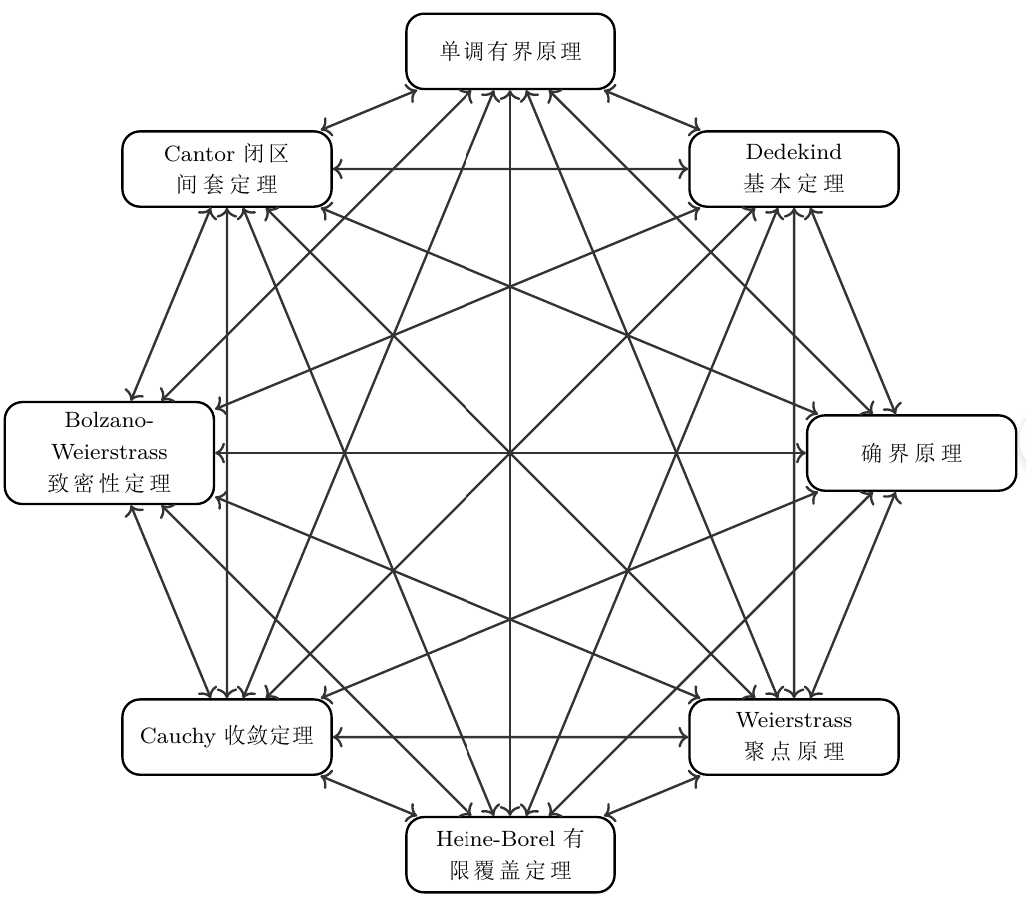
\includegraphics[width=0.6\linewidth]{figure/C2/1}
\end{center}
\newpage
% 第1节：拓扑空间与开闭集
% !TEX root = ../../../main.tex
% 所属：第一部分：单变量分析学 / 第3章：实数的八大基本定理
% 节：3.1 拓扑空间与开闭集
% 正文按原文件顺序保存；由 ../chapter3.tex 调用。
\section{拓扑空间与开闭集}
\begin{definition}\label{defoftosp}
	令$X$是一个集合.$X$的拓扑$\mathcal{T}$是由$X$的一些子集所构成的族，且$\mathcal{T}$满足
	\begin{enumerate}
		\item $X\in \mathcal{T}$且$\varnothing\in\mathcal{T}$
		\item $\mathcal{T}$ 中集合的任意并仍属于 $\mathcal{T}$
		\item $\mathcal{T}$中集合的有限交仍属于$\mathcal{T}$
	\end{enumerate}
	称偶对$\left(\mathrm{X}, \mathcal{T}\right)$ 是一个拓扑空间.
\end{definition}
\begin{definition}
	$\left(\mathrm{X}, \mathcal{T}\right)$ 是一个拓扑空间,那么$\mathcal{T}$中的元素在$\mathrm{X}$中称做开的，换言之$\mathcal{T}$中的元素称为$\mathrm{X}$中的开集.
	
	闭集定义为开集关于$\X$的补集.
	
	在$\left(\mathrm{X}, \mathcal{T}\right)$ 中存在即是开集又是闭集的集，称为闭开集.
\end{definition}
\begin{proposition}
	对拓扑空间$\left(\mathrm{X}, \mathcal{T}\right)$
	
	（1）$\mathrm{X}$ ，$\varnothing$ 是团开的
	
	（2）开集的任意并仍是开集
	
	（3）开集的有限交仍是开集
	
	（4）闭集的任意交仍是闭集
	
	（5）闭集的有限并仍是闭集
\end{proposition}
\begin{proof}
	$(1),(2),(3)$由开集的定义是显然的，对$(4),(5)$使用De Morgan定理,设$S_{\alpha}\in\mathcal{T}$,那么$S_{\alpha}^C$是闭集，则
	$$\bigcap_\alpha S_\alpha^C=\left(\bigcup_\alpha^n S_\alpha\right)^C \text {, 而 }\bigcup_\alpha^n S_\alpha  \in \mathcal{T}$$
	$$	\bigcup_{i=1}^n S_i^C=\left(\bigcap_{i=1}^n S_i\right)^C \text {, 而 } \bigcap_{i=1}^n S_i \in \mathcal{T}$$
\end{proof}
\begin{example}
	\begin{enumerate}
		\item		$\mathrm{X}=  \{a, b, c, d, e, f\}$,令
		$$\mathcal{T}_1=\{\mathrm{X}, \phi,\{a\},\{c, d\},\{a, c, d\},\{b, c, d, e, f\}]$$
		显然地，$\mathcal{T}_1$是$\mathrm{X}$上的一个拓扑：其中
		\begin{itemize}
			\item $\{a\}$是闭开的
			\item$\{b,c\}$既不是闭的，也不是开的是开的，而不是闭的
			\item$\{c,d\}$
			\item$\{a, b, e, f\}$ 是闭的，而不是开的
		\end{itemize}
		\item 离散拓扑$\T$,对集合$\mathrm{X}$,$\T$定义为$\mathrm{X}$所有子集构成的族.显然的，$\mathrm{X}$的任意子集都是闭开的.
		\item 平凡拓扑$\T_0$,定义为
		\[\T_0:=\{\mathrm{X},\varnothing\}\]
	\end{enumerate}
\end{example}
\begin{theorem}
	$f:X\rightarrow Y$,是一个从$X$到$Y$的$1-1$映射，且是满射，令$\left(\mathrm{X}, \mathcal{T}\right)$是一个拓扑空间，设$\T_1=\{f(S):S\in\T\}$,则$\T_1$是$\mathrm{Y}$上的一个拓扑
\end{theorem}
\begin{proof}
	（1）
	
	由 $\mathrm{X} \in \T,  \Y=f(\mathrm{X} )$ 得 $\Y\in \T_1$
	
	由 $\varnothing \in \T,  \varnothing=f(\varnothing)$ 得 $\varnothing \in \T_1$
	
	（2）$A_\alpha \in \T$ ，则 $f\left(A_\alpha\right) \in \T_1$ ，那么考虑
	
	$$
	\bigcup_\alpha f\left(A_\alpha\right)=f\left(\bigcup_\alpha A_\alpha\right) \in \mathcal{T}_1
	$$
	
	(3)$A_n \in \T$则$f\left(A_n\right) \in \T_1$考虑
	
	$$\bigcap_{k=1}^n f\left(A_k\right)=f\left(\bigcap_{k=1}^n A_k\right) \in \T_1$$
\end{proof}
%
% 第2节：Euclidean拓扑与拓扑基
% !TEX root = ../../../main.tex
% 所属：第一部分：单变量分析学 / 第3章：实数的八大基本定理
% 节：3.2 Euclidean拓扑与拓扑基
% 正文按原文件顺序保存；由 ../chapter3.tex 调用。
\section{Euclidean拓扑与拓扑基}
\begin{definition}[$\R$上的Euclidean拓扑]\label{defofeuto}
	$\R$上的一个子集$S$在$\R$上的Euclidean拓扑里被称为是开的，若其有以下性质:
	$$\forall x\in S,\exists a,b\in\R~\textbf{且}~a<b,~\text{使得}~x\in\left(a,b\right)\subset S$$
\end{definition}
注意：在此之后，我们说拓扑空间$\R$,默认为Euclidean拓扑
\begin{proposition}
	\ref{defofeuto}中定义的Euclidean拓扑是一个拓扑
\end{proposition}

\begin{proof}
	（i）$\forall x \in \mathbb{R}$ ，取 $a=x-1, b=x+1,  x \in\left(x-1,  x+1\right)\subset \mathbb{R}$ ，故 $\mathbb{R} \in \T$
	由空真原理，$\varnothing \in \T$
	
	（ii）令 $A_\alpha \in \T$ ，下证 $\bigcup_\alpha A_\alpha \in \T$ ，也即 $\bigcup_\alpha A_\alpha$ 具备\ref{defofeuto}中的性质
	
	取 $x \in \bigcup_\alpha A_\alpha$ ，那么 $\exists k$ ，使得$x \in A_k$ ，$\exists a, b \in \mathbb{R}$ 且 $a<b$ ，使得
	
	$$
	(a, b) \subset A_k \subset \bigcup_\alpha A_\alpha
	$$
	
	
	得证
	
	(iii）考虑 $A_1 \cap A_2$ 的情况，有限交 可以由归纳法得.
	
	取 $A_1, A_2 \in \T$ ，令 $y \in A_1 \cap A_2$ ，则 $y \in A_1, \exists a, b \in \mathbb{R}$ 且 $a<b$ ，使得
	
	$$
	y \in(a, b) \subset A_1
	$$
	
	
	同理 $y \in A_2, \exists c, d \in \mathbb{R}$ ，且 $c<d$ ，s．t．
	$$y \in(c, d) \subset A_2$$
	取 $e=\max \{a, c\}, \quad f=\min \{b, d\}$ ．那么
	
	$$
	y \in(e, f) \subset A_1 \cap A_2
	$$
	
	
	得证
\end{proof}
\begin{proposition}
	对拓扑空间$\R$，我们有以下陈述
	
	（1）开区间$\left(r,s\right)$是开集
	
	（2）区间 $(r,+\infty),(-\infty, r)$ 是开集
	
	（3）闭区间 $[c, d]$ 不是开集而是闭集
	
	（4）单元集 $\{a\}$ 是闭集
	
	（5）$\Z$是闭集
	
	（6）$\Q$不是闭集也不是开集
\end{proposition}
\begin{proof}
	（1）$\forall x \in(r, s)$ ，取 $a=r, b=s$ ，那么 $x \in(a, b) \subset(r, s)$
	
	(2)$\forall x \in(r,+\infty)$ ，取
	
	$$
	x \in(r, x+1) \subset(r,+\infty)
	$$
	
	$\forall y \in(-\infty, r)$ ，取
	
	$$
	y \in(y-1, r) \subset(-\infty, r)
	$$
	
	
	(3)对 $x=c \in[c, d]$ ，假设 $\exists a, b \in \mathbb{R}$ ，使得$c \in(a, b) \subset[c, d]$ ，那么 $a<c<b$ 且 $a<\dfrac{a+c}{2}<c<b$,
	因此 $ \dfrac{a+c}{2} \in(a, b)$ 而 $\dfrac{a+c}{2} \notin[c, d]$ ，矛盾，因此 $[c, d]$ 不是开集.
	
	取 $(-\infty, c) \cup(d,+\infty)$ 为开集，其余集 $[c, d]$ 为闭集
	
	
	(4)考虑$S=\left(-\infty,a\right)\bigcup\left(a,+\infty\right)$为开集，则$S^C=\{a\}$为闭集.
	
	(5)$\Z^C=\bigcup\limits_{n\in\Z}(n,n+1)$是开集，则$\Z$为闭集
	
	(6)若$\Q$为开集，$\left(\forall x\in\Q\right)\left(a,b\in\R\right),$使得$x\in\left(a,b\right)\subset\Q$,$\exists q\in\R\setminus\Q$,同上，$\R\setminus\Q$也不是开集，故$\Q$不是闭集.
\end{proof}
\begin{theorem}
	$\R$的子集$S$是开的，当且仅当$S$是某些开集的并.
\end{theorem}
\begin{proof}
	必要性：$S$ 是开的，$\forall x \in S, \exists I_x=(a, b)$ 使得$x \in I_x \subset S$ 下证
	$$S=\bigcup_{x \in S} I_x$$
	
	（i）$S \subset \bigcup_{x \in S}I_x$
	
	令 $y \in S$ ．则 $y \in I_y \subset \bigcup_{x \in S} I_x$ ，那么 $S \subset \bigcup_{x \in S} I_x$
	
	（ii）$\bigcup_{x \in S }I_x \subset S$
	
	令 $z \in \bigcup_{x \in S} I_x$ ，$\exists t \in S$ ，使得$z \in I_t$ ．而 $I_t \subset S$ ．故 $z \in S$ ，则 $\bigcup_{x \in S} I_x\subset S$
	
	综上
	
	$$
	S=\bigcup_{x \in S} I_x
	$$
	
	
	充分性 :$S=U_{j \in J}\left(a_j, b_j\right)$ ，而$\left(a_j, b_j \right)$开，那么 $S$ 开
\end{proof}
\begin{definition}
	$\left(\X,\T\right)$是一个拓扑空间，由 $\X$ 中的开集组成的族 $\mathcal{B}$被称为是 $\T$ 的基，若 $\X$ 中的任意开集是 $\mathcal{B}$ 中元素的并.
\end{definition}
例：$\R$上的Euclidean拓扑的标准基定义为

$$
\B=\{(a, b): a, b \in \mathbb{R}, a<b\}
$$
也就是$\B$是所有开区间的族.

离散空间$\left(\X,\T\right)$的基可以定义为

$$
\B=\{\{x\}: x \in \X\}
$$

显然易见的，$\T$ 本身是它自己的一个基.若$\B$是 $\T$ 的一个基，$\B_1$ 是一个组，满足 $\B \subset \B_1 \subset \T$ ，那么 $\B_1$ 也是 $\T$ 的一个基.

\begin{proposition}
	\label{eq_of_2def_tpbas}
	令$\X$是一个非空集，且令$\B$是$\X$中某些子集所构成一个族那么 $\B$ 是 $\X$ 的拓扑 $\T$ 的基当且仅当 $\B$ 有如下的性质：
	
	（a）$\X=\bigcup\limits_{B \in \B }B$
	
	（b）$\forall B_1, B_2 \in \B, B_1 \cap B_2$ 是 $\B$ 中元素的并
\end{proposition}


\begin{proof}
	必要性：已知 $\B$ 是$\X$的拓扑 $\T$ 的一个基，那么 $\T$ 满足\ref{defoftosp}中的（i）（ii） （iii）．$\X \in \T$ ，$\X$是开集，根据 $\B$ 的定义$(a)$ ， $(b)$ 得证.
	
	充分性：已知$\B$满足性质（a），（b），使$\T$是由$\B$中元素的并形成的 $\X$ 的所有子集（称$\T$为由$\B$生成的拓扑）
	
	$$
	T=\left\{U \subset \X: U=\bigcup_{B \in \B} B\right\}
	$$
	
	
	下证 $\T$ 是一个拓扑，满足 \ref{defoftosp} 中的（i）（ii）（iii）．
	
	（i）由（a），$\X \in \T$ ，
	而 $\varnothing$ 是 $\B$ 中元素的空并，故$\varnothing \in \mathcal{T}$
	
	（ii）考虑 $T_\alpha \in \T$ ，而每一个 $T_\alpha$ 都为$\B$中元素的并，$\T_\alpha$ 的任意并也为 $\B$ 中元素的并，$\bigcup_\alpha T_\alpha \in \T$
	
	（iii）考虑 $C, D \in \T$ ，则
	
	$$
	C=\bigcup_{k \in K} B_k, D=\bigcup_{j \in J} B_j, K,J \text { 为任意指标集 }
	$$
	
	
	那么
	
	$$
	C \cap D=\left(\bigcup_{k \in K} B_k\right) \cap\left(\bigcup_{j \in J} B_j\right)=\bigcup_{\substack{k \in K \\ j \in J}}\left(B_k \cap B_j\right)
	$$
	
	
	由（b），$C \cap D \in \T$
	
	由归纳法，有限交属于$\T$.
\end{proof}
$\mathbb{R}$ 上闭区间 $[a, b]$ 的 Euclidean 拓扑.
$$\T=\left\{(c, d): a<c<d<b\right\} \cup\left\{[a, e): a<e<b\right\} \cup\left\{(f, b]: a<f<b\right\}$$


$\mathbb{R}^* $ 的 Euclidean 拓扑,其中 $\mathbb{R}^*=[-\infty,+\infty]$
$$\T=\{(a, b):-\infty<a<b<+\infty\}\cup\{[-\infty, c):-\infty<c<-\infty\}\cup\{(d,+\infty]:-\infty<d<+\infty\}$$

$\mathbb{R}^n$ 上的 Euclidean 拓扑的基定义为

$$
\B=\left\{\left(x_1, \cdots, x_n\right) \in \mathbb{R}^n: a_i<x_i<b_i, i=1,2, \cdots, n\right\}
$$
\begin{proposition}
	\label{th:tp_subset}
	对拓扑空间$(\X,\T)$，$\X$的子集构成的族 $\B$ 是 $\T$ 的一个基当且仅当 任对开集 $U$ 中的任何点 $x$ ，存在 $ B \in \B$ 使 得 $x \in B \subset U$ .
\end{proposition}

\begin{proof}
	必要性：已知 $\B$ 是 $\T$ 的一个基，且 $x \in U \in \T$ .由于$U$是一个开集
	
	$$
	U=\bigcup_\alpha B_\alpha, B_\alpha \in \B
	$$
	
	$x \in U$ 则 $\exists j$ ，使得$x \in B_j \subset U$
	
	充分性：已知 $\forall$ 开集 $U$ 中任意点 $x$ ，存在 $B_x \in \B$ 使得 $x \in B_x \subset U$ ，断言
	
	$$
	U=\bigcup_{x \in U} B_x
	$$
	
	
	也即任何开集可以写成 $\B$ 中元素的并.
	
	（i）$U \subset \bigcup_{x \in U} B_x$
	
	$y \in U$ ，$\exists B_y \in B$ 使得$y \in B_y$ ，而 $B_y \subset \bigcup_{x \in U} B_x$ ，故 $y \in U_{x \in U} B_x$ ，即 $U \subset \bigcup_{x\in U} B_x$
	
	（ii）$\bigcup_{x \in U} B_x \subset U$
	
	$z \in \bigcup_{x \in U} B_x$ ，$\exists t \in U$ ，使得$z \in B_t \subset U$ ，故 $z \in U$ ，即 $\bigcup_{x \in U} B_x \subset U$
	
	综上
	
	$$
	U=\bigcup_{x \in U} B_x
	$$
\end{proof}
上面$U=\bigcup_{x \in U} B_x$的证明在以后尝尝用到，我们省略.
\begin{corollary}\label{2.2.8}
	对$(\X,\T)$,$\B$是其拓扑基，那么$\X$的子集$V$是开的当且仅当$(\forall x\in V)(\exists B\in\B),\text{使得}x\in B\subset U$
\end{corollary}
\begin{proof}
	必要性由(\ref{th:tp_subset})得证
	
	充分性:$(\forall x\in V)(\exists B_x\in \B)\text{使得}x\in B\subset V$,那么$V=\bigcup_{x\in V}B_x\in\T$.故$V$是开集
\end{proof}
\begin{corollary}
	$\B_1$ 和 $\B_2$ 分别是 $\T_1$ 和 $\T_2$ 的基，那么 $\T_1=\T_2$ 当且仅当
	
	（i）$\forall B \in \B_1, \forall x \in B, \exists B^{\prime} \in \B_2$ ，使得$x \in B^{\prime} \subset B$
	
	（ii）$\forall B \in \B_2, \forall x \in B, \exists B^{\prime} \in \B_1$ ，使得$x \in B^{\prime} \subset B$
	
\end{corollary}
\begin{proof}
	必要性：$\T_1=\T_2$ ，由 \ref{2.2.8}（i）（ii）易得
	
	充分性：$\B_1, \B_2$ 满足（i）（ii），由\ref{2.2.8}
	（i）说明 $B \in \B_1$ 在 $\left(\X, \T_2\right)$ 上是开的，$\B_1 \subset \T_2$ .因为 $\T_1$ 中的每一个元素都是 $\T_2$ 中元素的并，得 $\T_1 \subset \T_2$ .同理，由（ii）$\T_2 \subset \T_1$
	
	综上 $\T_1=\T_2$
\end{proof}

%
% 第3节：极限点，邻域与连通性
% !TEX root = ../../../main.tex
% 所属：第一部分：单变量分析学 / 第3章：实数的八大基本定理
% 节：3.3 极限点，邻域与连通性
% 正文按原文件顺序保存；由 ../chapter3.tex 调用。
\section{极限点，邻域与连通性}
\begin{definition}\label{defoflimpoint}
	设$A$为拓扑空间$(\X,\T)$的子集，把拓扑空间中的元素称为点，点$x\in\X$称为$A$的极限点(聚点)，若每个包含$x$的开集$U$中包含$A$中不同于$x$的一个点.
\end{definition}
\begin{proposition}
	令 $A$ 为拓扑空间 $(\X, \T)$ 的一个子集. $A$ 在 $(\X, \T)$ 中是闭的当且仅当 $A$ 包含它所有的极限点.
\end{proposition}

\begin{proof}
	必要性：已知 $A$ 在$(\X, \T)$中是闭的.若存在一个 $A$ 的极限点不属于 $A$ ，换言之，存在一个 $A$ 的极限点 $p, p \in A^C$ 且 $A^C$ 是开集，由极限点的定义，$A^C$ 中有一个$A$中不同于 $x$ 的点，矛盾.
	
	充分性：$\forall z \in A^C$ ，$z$ 不是 $A$ 极限点，$\exists$ 开集 $U_z(z\in U_z)$ ，使得．$U_z \cap A=\varnothing$也即 $U_z\subset A^C$ ，因此 $A^C=\bigcup\limits_{z \in A^C} U_z$ ，$A^C$ 是开集的并因此也是开的，因此补集 $A$ 是闭的
\end{proof}
\begin{proposition}
	令$A$为$(\X,\T)$的子集并且$A^{\prime}$是$A$的所有的极限点构成的集合，则$A\cup A^{\prime}$是闭集
\end{proposition}

\begin{proof}
	只需证$A\cup A^{\prime}$包含它本身所有的极限点即可
	
	如不然，$\exists p$是$A\cup A^{\prime}$的极限点，但$p\in(A\cup A^{\prime})^C$
	
	设$p\in(A\cup A^{\prime})^C$，由$p\notin A^{\prime}$,得$p$不是$A$的极限点，$\exists$开集$U,p\in U$,使得
	
	\[U\cap A=\{p\}\text{或}\varnothing\]
	而$p\notin A$,故$U\cap A=\varnothing$
	
	同理，$p$不是$A^{\prime}$的极限点，且$p\notin A^{\prime}$,可以使上述的$U\cap A^{\prime}=\varnothing$
	
	那么$U\cap(A\cup A^{\prime})=\varnothing,p\in U$
	
	如此，$p$不是$A\cup A^{\prime}$的极限点，$A\cup A^{\prime}$是闭集
\end{proof}
\begin{definition}
	$A$ 是 $(\X, \T)$ 的子集，$A^{\prime}$ 是 $A$ 所有极限点的集合，称 $A \cup A^{\prime}$是 $A$ 的闭包，记为 $\bar{A}$
	
	
\end{definition}
\begin{definition}
	$A$ 是 $(\X, \T)$ 的子集，$A$ 在 $\X$ 中处处稠密，若 $\bar{A}=\X$
\end{definition}
\begin{proposition}
	$\mathbb{Q}$ 在 $\mathbb{R}$ 中处处稠密
	
\end{proposition}
\begin{proof}
	只需 $\overline{\mathbb{Q}}=\mathbb{R}$ ，若 $\overline{\mathbb{Q}} \neq \mathbb{R}, \exists x \in \mathbb{R}\setminus \overline{\mathbb{Q}}$ .由 $\mathbb{R}\setminus \overline{\mathbb{Q}}$ 在$\R$中是开的 ,$\exists(a, b) \subset \R\setminus \overline{\mathbb{Q}}$ .但是在每一个$(a, b)$ 存在一个 $ q \in \mathbb{Q}$ ，那么
	
	$$
	q \in(a, b) \subset \mathbb{R}\setminus \overline{\mathbb{Q}} \Rightarrow q \subset \mathbb{R}\setminus \mathbb{Q}
	$$
	
	
	矛盾.
\end{proof}
显然地，若 $A$ 在 $\X$ 中稠密则 $A^C$ 中全部是 $A$ 的极限点.
\begin{proposition}
	$A$ 是$(\X,\T)$的子集，$A$ 在 $\X$ 中稠密当且仅当 $\forall U \in \T$且 $U\neq \varnothing, A \cap U \neq \varnothing$
\end{proposition}

\begin{proof}
	必要性：已知 $A$ 在$\X$中处处稠密，则 $A \cup A^{\prime}=\X$
	
	假设 $U \cap A=\varnothing . \forall x \in U, x \notin A$ 则 $x$ 不是 $A$ 的极限点，这与 $A^C$ 中全部是 $A$的极限点矛盾.
	
	充分性：己知 $\forall U \in\T$ 且 $U \neq \varnothing, A \cap U \neq \varnothing$
	
	若 $A=\X$ ，显然 $A$ 在$\X$中稠密
	
	若 $A \neq \X$ ，设 $x \in A^C$ .如果 $U \in \T$ ，且 $x \in U$ ，那么 $U \cap A \neq \varnothing$ ，于是 $x$ 是 $A$ 的一极限点. $\forall x \in A^C$ ，$x$ 都是 $A$ 的极限点，也即 $x \in A^{\prime}$ ，于是 $A^C \subset A^{\prime}$ ，则 $\bar{A}=A^{\prime} \cup A=\X$
	
\end{proof}
\begin{definition}
	$(\X,\T)$是一个拓扑空间，$N$ 是 $
	\X$ 的子集且 $p \in N$ .若对 $p$ ，存在一个开集$U$，使得，$p \in U \subset N$ ，称 $N$ 为 $p$ 的邻域.
\end{definition}
\begin{proposition}
	$A$ 是$(\X,\T)$的子集，点 $x \in \X$ 是 $A$ 的极限点当且仅当 $x$ 的每个邻域包含一个不同于$\X$属于$A$的点
	
\end{proposition}

\begin{proof}
	根据定义显然
\end{proof}
\begin{corollary}
	
	（1）$A$ 是 $(\X, \T)$ 的子集，$A$ 是闭的当且仅当 $\forall x \in A^C$ ，$\exists x$ 的邻域 $N$满足 $N \subset A^C$
	
	（2）$U$是$(\X, \T)$ 的子集，$U$是开的当且仅当 $\forall x \in U$ ，$\exists x$ 的邻域满足$N\subset U$
	
	（3）$U$是$(\X, \T)$ 的子集，$U \in \T$ 当且仅当 $\forall x \in U, \exists V \in \T$ ，使得$x \in V\subset U$
\end{corollary}
\begin{definition}
	在 $\mathbb{R}$ 上，球型邻域定义为
	
	$$
	\left(x_0-\delta, x_0+\delta\right)
	$$
	
	
	记为 $N\left(x_0, \delta\right)$ 或 $O\left(x_0, \delta\right)$ 
	
	下文中，在 $\mathbb{R}$上 的邻域默认为球型邻域
\end{definition}
\begin{lemma}
	$S$是$\R$上有界的子集，$S$是闭的则$p=\sup S\in S$
\end{lemma}
\begin{proof}
	设$p\in S^C$,$S^C$是开的，故$\exists(a,b)$,使得$p\in(a,b)\subset S^C$
	
	$p=\sup S$,而$a<p$.$\exists x\in S$,使得$x>a$,且$x<p<b$,那么$x\in(a,b)\subset S^C$,矛盾
\end{proof}
\begin{definition}
	对$(\X,\T)$,称$X$是连通的，若闭开集只用$\X$与$\varnothing$
\end{definition}
\begin{proposition}
	\label{con_of_R}
	$\R$是连通的
\end{proposition}

\begin{proof}
	也即 $\mathbb{R}$ 上的闭开集只有 $\mathbb{R}$ 与 $\varnothing$
	
	假设 $T \neq \mathbb{R}$ 且 $T \neq \varnothing$ ，且$T$ 是闭开的. $\exists x \in T,  z \in T^c$
	不失一般性， 假设 $x<z$ .令 $S=T \cap[x, z]$ ，$S$ 是闭的.
	
	$z$ 是 $S$ 的上界，$S$ 有上确界，令 $p=\sup S$ ，故 $p \in S$ ，因此 $p \in[x, z], p \leqslant z$，又 $p \in T, z \in T^c, p \neq Z$ 故 $p<Z$ .
	
	又 $T$ 是开集，$p \in T . \exists(a, b), p \in(a, b)\subset T$
	
	取 $t$,使得$p<t<\min (b, z)$ ，有 $t \in T$ 且 $t \in[p, z]$
	
	因此 $t \in T \cap[x, z]=S$ ，而 $t > p=\sup S$ ，矛盾
	
	故 $T=\mathbb{R}$ 或 $\varnothing$
\end{proof}

%
% 第4节：同胚关系与同胚映射
% !TEX root = ../../../main.tex
% 所属：第一部分：单变量分析学 / 第3章：实数的八大基本定理
% 节：3.4 同胚关系与同胚映射
% 正文按原文件顺序保存；由 ../chapter3.tex 调用。
\section{同胚关系与同胚映射}

\begin{definition}
	令 $Y$ 是 拓扑空间 $(\X, \T)$ 的一个非子集.族 $\T_Y=\{O \cap Y: O \in \T\}$ 由 $Y$ 的子集组成，是一个定义在 $Y$ 上的拓扑,称之为子空间拓扑，$\left(Y, \T_Y\right)$ 称为 $(\X, \T)$ 的子空间
\end{definition}
\begin{definition}
	对$(\X,\T_1),(Y,\T_2)$,若函数$f:\X\rightarrow Y$满足：
	
	（i）$f$ 是$1-1$的且是满射
	
	（ii）$\forall U \in \T_2, f^{-1}(U) \in \T_1$
	
	（iii）$\forall V \in \T_1, f(V) \in \T_2$
	
	就称 $\left(x, \T_1\right),\left(Y, \T_2\right)$ 是同胚的.称 $f$ 是 $\left(\X, \T_1\right),\left(Y, \T_2\right)$ 之间的一个同胚映射，记为 $\left(\X, \T_1\right)\cong\left(Y, \T_2\right)$
\end{definition}
\begin{proposition}
	同胚关系是一个等价关系.
\end{proposition}
\begin{proof}
	应有
	
	（1）$\left(\X, \T_1\right) \cong\left(\X, \T_1\right)$
	
	(2)$\left(\X, \T_1\right) \cong\left(Y, \T_2\right) \Leftrightarrow\left(\Y, \T_2\right) \cong\left(\X, \T_1\right)$
	
	（3）$\left(\X, \T_1\right) \cong\left(Y, \T_2\right),\left(Y, 
	\T_2\right) \cong\left(Z, \T_3\right) \Rightarrow\left(\X, \T_1\right) \cong\left(Z, \T_3\right)$
	
	只需验证恒等映射，逆映射，复合映射满足（i），（ii），（iii）即可.显然地，得证
\end{proof}
\begin{example}
	
	(a) $(0,1) \cong(a, b)$
	
	(b) $(-1,1) \cong \mathbb{R}$
	
	(c) $[a, b] \cong \mathbb{R}^*$
	
	(d) $[c, d) \cong(c, d]$
\end{example}
\begin{proof}
	（a）$f(x)=a(1-x)+b x$
	
	（i）显然地，$f$ 是 $1-1$ 的，且为满射
	
	
	(iii)	$$\begin{aligned}
		f((0,1) \text { 中开集}) & =f((0,1) \text { 中开区同的并 }) \\
		& =(a, b) \text { 中开区间的并 } \\
		& =(a, b) \text { 中开集 }
	\end{aligned}
	$$
	
	
	对（ii）考查 $f^{-1}$ 即可.
	
	故 $f$ 是 $(0,1) \rightarrow(a, b)$ 上的同胚映射.
	
	故 $(0,1) \cong(a, b)$
	
	（b）$$f(x)=\dfrac{x}{1-|x|}$$
	
	（c）考虑 $\left[-\dfrac{\pi}{2}, \dfrac{\pi}{2}\right]$ ，易知 $[a, b] \cong\left[-\dfrac{\pi}{2}, \dfrac{\pi}{2}\right]$
	
	$$
	\begin{gathered}
		f(x)=\tan ^{-1}(x) \quad x \in \mathbb{R}^* \\
		f: \mathbb{R}^* \rightarrow\left[-\dfrac{\pi}{2}, \dfrac{\pi}{2}\right]
	\end{gathered}
	$$
	
	（d）$f(x)=c+d-x$\end{proof}
\begin{theorem}
	同胚于连通空间的拓扑空间是连通的
\end{theorem}
\begin{proof}
	设 $\left(\X, \T_1\right) \cong\left(\Y, \T_2\right)$ ，已知 $\left(\X, \T_1\right)$ 连通，
	
	设 $\left(\Y, \T_2\right)$ 不连通，$\exists Y_1 \subset Y, Y_1 \neq Y$ 或 $\varnothing$ ，使得$Y_1$ 是闭开的，则 $f^{-1}\left(Y_1\right) \subset \X$ ，是 $\X$ 的闭开子集，矛盾，故 $\left(Y, \T_2\right)$ 连通 
\end{proof}

\begin{definition}
	$\mathbb{R}$ 中的子集 $S$ 称为区间，若它满足如下性质：也果 $x \in S$ ， $z \in S, y \in \mathbb{R}$ ，使得$x<y<z$ ，那 么$ y \in S$
\end{definition}

每个区间具下列形式之一：
\[\{a\},[a, b],(a, b),[a, b),(a, b],(-\infty, a),(-\infty, a],(a,+\infty),[a,+\infty),(-\infty,+\infty)\]

\begin{proposition}\label{2.4.7}
	$\R$的子空间$S$是连通的当且仅当$S$是一个区间
\end{proposition}
\begin{proof}
	充分性：证明类似于\ref{con_of_R} 略
	
	必要性：S是连通的，假定 $x \in S,  z \in S,  x<y<z$ ，且 $y \notin S$ .
	
	则 $(-\infty, y) \cap S=(-\infty, y] \cap S$ ，是 $S$ 的闭开子集,需证 $(-\infty, y) \cap S$ 是真且非空子集.由 $x \in S, x<y$ 得 $x \in(-\infty, y) \cap S$ ，它是真子集.由于 $z \in S$ ，但 $z \notin(-\infty, y) \cap S$ 于是 $S$ 不连通，矛盾
\end{proof}
\begin{theorem}
	$f:\left(\X, \T_1\right) \rightarrow\left(Y, T_2\right)$ 是同胚映射，令$a \in X$ ，考虑 $x\setminus \{a\}$与其子空间拓扑 $\T_1^{\prime}$ ，对 $f(a)$ ，考虑$Y\setminus \{f(a)\}$ 与其子空间拓扑 $\T_2^{\prime}$ ，则$(\X\setminus \{a\}, \T_1^{\prime})\text{与}\left(Y\setminus \{f(a)\}, \T_2^{\prime}\right)$ 同胚
\end{theorem}
\begin{proof}
	构造 $g:\left(X\setminus \{a\}, \T_1^{\prime}\right) \rightarrow\left(Y\setminus \{f(a)\}, \T_2^{\prime}\right)$ 即可，$g=f(x \neq a)$容易得$g$是一个同胚映射.
	
	
\end{proof}
\begin{corollary}
	
	（i）$(a, b)$不同胚于$[c, d)$
	
	（ii）$(a, b) $不同胚于 $[c, d]$
	
	（iii）$[a, b)$不同胚于$[c, d]$
	
\end{corollary}
\begin{proof}
	（i）：$X=[c, d),  Y=(a, b)$ ，假设 $X \cong Y$
	考虑 $X\setminus \{c\} \cong Y\setminus \{y\}$
	那么 $(c, d)$ 是一个区间，由\ref{2.4.7}, $(c, d)$ 是连通的，且 $Y\setminus \{y\}$ 是连通的，但 $(a, b)$ 去掉任何一个点都会导致它不连通，故$\X$不同胚于$Y$
	（ii），（iii）同理
\end{proof}
%
% 第5节：度量空间
% !TEX root = ../../../main.tex
% 所属：第一部分：单变量分析学 / 第3章：实数的八大基本定理
% 节：3.5 度量空间
% 正文按原文件顺序保存；由 ../chapter3.tex 调用。
\section{度量空间}
\begin{definition}
	$\X$ 是一个非空集，$d$ 是一个映射，定义在 $\X \times \X$ 上，$\forall a, b \in \X$ ，若满足
	
	（i）若 $a \neq b$ ，那么 $d(a, b)>0 ; d(a, a)=0$
	
	（ii）$d(a, b)=d(b, a)$
	
	（iii）$d(a, c) \leqslant d(a, b)+d(b, c)$
	
	那么 $d$ 称为 $\X$ 上的一个度量或者距离函数，$(\X, d)$ 称为度量空间. $d(a, b)$ 称为$a, b$ 之间的距离
\end{definition}
在$\R$上\[d(a,b)=|a-b|\]
称为$\R$上的Euclidean度量

在$\R^2$\[d((a_1,a_2),(b_1,b_2))=\sqrt{(a_1-b_1)^2+(a_2+b_2)^2}\]称为$\R^2$上的Euclidean度量
\begin{definition}
	令$(\X,d)$是一个度量空间，$r$ 是任意正实数.集合
	
	$$
	B_r(a)=\{x: x \in \X \text { 且 } d(a, x)<r\}	$$
	
	
	称为以 $a$ 为中心，$r$ 內为半径的开球
\end{definition}
\begin{lemma}
	令 $(\X, d)$ 是一个度量空间，且 $a, b \in \X . \delta_1, \delta_2 \in \mathbb{R}_{+}$若 $c \in B_{\delta_1}(a) \cap B_{\delta_2}(b), \exists \delta>0$ ，使得，$B_\delta(c) \subset B_{\delta_1}(a) \cap B_{\delta_2}(b)$
\end{lemma}
\begin{proof}
	取 $\delta=\min \left\{\delta_1-d(c, a), \delta_2-d(c, b)\right\}$ 即可
\end{proof}
\begin{corollary}\label{ints_of_ball}
	$(\X, d)$ 是一个度量空间，$B_1, B_2$ 是$(\X,d)$中的开球那么 $B_1 \cap B_2$ 是 $(X, d)$ 中一些开球的并集
\end{corollary}
\begin{proof}
	$\forall c \in B_1 \cap B_2$（假设不为 $\varnothing, \varnothing$ 下平凡）.
	
	$\exists \delta(c)$ ，使得，$B_{\delta(c)}(c) \subset B_1 \cap B_2$ ，
	
	那么
	
	$$
	B_1 \cap B_2=\bigcup_{x \in B_1 \cap B_2} B_{\delta(x)}(x)
	$$
\end{proof}
显然的，我们有以下的命题
\begin{proposition}
	令 $(\X, d)$ 是一个度量空间．那么 $(\X, d)$ 中所有开球构成一个族，是$\X$中一个拓扑的拓扑基
\end{proposition}
\begin{proof}
	由\ref{eq_of_2def_tpbas}与\ref{ints_of_ball}得
\end{proof}
称$\T$为度量$d$诱导出的拓扑
\begin{proposition}
	$(\X,d)$是一个度量空间，$\T$是由$d$诱导出的拓扑，$(\X,\T)$的子集$U$是开的，当且仅当$(\forall a\in U)(\exists \varepsilon>0),$使得$B_\varepsilon(a)\subset U$
\end{proposition}
\begin{proof}
	必要性：$U \in\T$ ，所有开球是一个拓扑基.
	
	$$
	U=\bigcup_{x \in U} B_{\delta(x)}(x)
	$$
	
	
	对 $a, \varepsilon=\delta(a), a \in B_{\varepsilon}(a) \subset U$
	
	充分性：这等价于 $\quad U=\bigcup_{a \in U} B_{\varepsilon(a)}(a)$
	
	说明$U$是开的.
\end{proof}
\begin{definition}
	$(\X,\T)$是一个拓扑空间，$A$是其任意子集. $A$ 包含的最大的那个开集称为 $A$ 的内部，记为 $\operatorname{Int}(A)$ . $\forall x \in \operatorname{Int}(A), x$ 称为 $A$ 的内点.
	
	$\operatorname{Int}\left(A^c\right)$ 定义为 $A$ 的外部，其任何点称为 $A$ 的外点，外部记为$\operatorname{Ext}A $
	
	$A$ 的边界定义为 $\bar{A}\setminus\operatorname{In} t(A)$ ，记为 $\partial A$ ，其点称为 $A$ 的边界点
\end{definition}

%
% 第6节：紧集，Cantor集与Heine-Borel定理
% !TEX root = ../../../main.tex
% 所属：第一部分：单变量分析学 / 第3章：实数的八大基本定理
% 节：3.6 紧集，Cantor集与Heine-Borel定理
% 正文按原文件顺序保存；由 ../chapter3.tex 调用。
\section{紧集，Cantor集与Heine-Borel定理}
\begin{definition}
	$\mathcal{O}=\left\{O_i\right\}$是$\X$子集构成的族，$i \in I$ ，$I$是指标集．$A$是 $\X$的一个子集.则若
	
	$$
	A \subset \bigcup_{i \in I} O_i
	$$
	
	
	称 $O_i, i \in I$ 为 $A$ 的覆盖.
	
	若上述定义中的 $O_i$ 为 $(\X, \T)$ 中的开集，则 $O_i, i \in I$ 称为 $A$ 的一个开覆盖.
	
	将$O_i, i \in I$ 的有限子族$O_{i_1}, O_{i_2}, \cdots, O_{i_n}$  称 $A$ 的有限子覆盖.若 $A \subset O_{i_1} \cup O_{i_2} \cup \cdots \cup O_{i_n}$
\end{definition}
\begin{definition}
	$(\X,\T)$的子集$A$被称为是紧的，若$A$的任意开覆盖存在一个有限子覆盖.
	
	若$(\X,\T)$的紧子集$A=\X$,则称$(\X,\T)$是紧空间
\end{definition}
\begin{proposition}
	$f:(\X,\T_1)\rightarrow(\Y,\T_2)$是一个同胚映射，若$(\X,\T_1)$是紧空间，则$(\Y,\T_2)$紧空间.
\end{proposition}
\begin{proof}
	$\forall\left\{U_i\right\}_{i\in I}$ 使得，
	$$U_i \in \T_2$$且 $$\Y \subset \bigcup_{i \in I} U_i$$
	
	由 $f$是一个同胚，$f^{-1}\left(U_i\right) \in \T_1$,$\forall x \in \X, f(x) \in \Y . f(x)$ 必属于某 $U_j$ ，故 $x \in f^{-1}\left(U_j\right)$
	于是 $\left\{f^{-1}\left(U_i\right)\right\}_{i \in I}$ 是$\X$的一个开覆盖.
	
	由$X$紧，存在有限子覆盖.
	$$\X\subset f^{-1}(U_{i_{1}})\cup\cdots\cup f^{-1}(U_{i_{n}})$$
	则
	$$\Y=f(\X)\subset U_{i_{1}}\cup\cdots\cup U_{i_{n}}$$
	
	
	于是$\Y$是紧空间.
	
\end{proof}
\begin{theorem}[Heine-Borel 定理]\label{HB_Th}
	$\R$的子集是紧的当且仅当该子集为有界闭集
\end{theorem}
在证明\ref{HB_Th}之前我们先做一些准备工作.
\begin{proposition}
	$\left[0,1\right]$是紧的
\end{proposition}
\begin{proof}
	$O_i, i \in I$ 是 $[0,1]$ 的一个开覆盖. $\forall x \in[0,1], \exists O_i$ 使得$x \in O_i$ ．而$O_i$是开的,存在在 $[0,1]$ 中开的区间 $U_x$，使得$x \in U_x \subset O_i$
	
	定义 $[0,1]$ 的子集 $S$：
	$$S=\left\{z:\left[0, z\right] \textbf{可以被有限个} U_x \textbf{覆盖} \right\}$$
	也即 $z \in S \Rightarrow\left[0, z\right] \subset U_{x_1} \cup U_{x_2} \cup \cdots \cup U_{x_n}$ ,对某些 $x_1, \cdots, x_n$ 
	
	现在，令 $x \in S$ 和 $y \in U_x$ .那么 $U_x$ 是一个包含 $x$ 和 $y$ 的区间.
	
	$[x, y] \subset U_x .(\textbf{不失一般性} x \leqslant y)$ 所以
	
	$$
	[0, y] \subset U_{x_1} \cup U_{x_2} \cup \cdots \cup U_{x_n} \cup U_x
	$$
	
	
	因此 $y \in S$ ．
	
	$
	\forall x \in[0,1], U_x \cap S=U_x \text { 或 } \varnothing
	$
	
	
	这说明
	
	$$
	S=\bigcup_{x \in S} U_x
	$$
	
	
	并且
	
	$$
	[0,1]\setminus S=\bigcup_{x \notin S} U_x
	$$
	
	
	因此，$S$ 既是开的，也是闭的在 $[0,1]$ 中，由 $[0,1]$ 的连通性，$S=[0,1]$ 或 $\varnothing$
	
	而 $0 \in S$ ，故 $S=[0,1]$ ，这就是说 $[0,1]$ 可以被有限个 $U_x$覆盖.故 $[0,1] \subset U_{x_1} \cup \cdots \cup U_{x_m} \subset O_{i_1} \cup \cdots \cup O_{i_m}$ ，因此 $[0,1]$ 是紧的.
	
	
\end{proof}
由同胚映射对紧性的保持，$\left[a,b\right]$也是紧的.
\begin{proposition}
	任何紧空间的闭子集都是紧的.
\end{proposition}
\begin{proof}
	令 $A$ 是紧空间$(\X,\T)$的一个闭子集.今 $U_i \in \T, i \in I$ 是 $A$ 的任意开覆盖,那么
	
	$$
	\X \subset\left(\bigcup_{i \in I} U_i\right) \cup(\X\setminus A)
	$$
	
	
	而$\X$紧，故存在 $i_1, \cdots, i_k $使得
	
	$$
	\X \subset U_{i_1} \cup U_{i_2} \cup \cdots \cup U_{i_k} \cup(X\setminus A)
	$$
	
	
	那么
	
	$$
	A \subset U_{i_1} \cup U_{i_2} \cup \cdots \cup U_{i_k}
	$$
	
	
	因$A \cap(X\setminus A)=\varnothing$ ,故 $A$ 是紧的
\end{proof}
现在我们回归到\ref{HB_Th}的证明
\begin{proof}
	对有界闭的集合 $A$ ，必存在区间 $[a, b]$ ，使得$A \subset[a, b]$, $A$是紧空间$\left[a,b\right]$的闭子集,故$A$是紧的.
	
	下面,已知$A$是$\R$的紧子集，证明$A$是有界闭集
	
	$(i)$紧$\Rightarrow$有界
	
	A是紧的，取开覆盖
	
	$$
	\{(-n, n): n \in \mathbb{N}\}
	$$
	
	
	存在有限子覆盖
	$$A \subset\left(-n_1, n_1\right) \cup \cdots \cup\left(-n_k, n_k\right)$$
	令 $N=\max \left\{n_1, \cdot, n_k\right\}$．
	
	$$A \subset(-N, N) \subset \left[-N,N\right]$$
	故A有界.
	
	$(ii)$紧$\Rightarrow$闭
	
	只需证 $A$ 包含其所有极限点，也即若 $x \notin A$ ，则存在包含 $x$ 的开集与 $A$交集为空集.
	
	取定 $x \notin A$ ，对每个 $y \in A$ ，令 $\varepsilon_y=\dfrac{|x-y|}{2}>0$
	取开集
	
	$$
	U_y=\left(y-\varepsilon_y, y+\varepsilon_y\right), \quad V_y=\left(x-\varepsilon_y, x+\varepsilon_y\right)
	$$
	
	
	则 $U_y \cap V_y=\varnothing$
	
	$\left\{U_y\right\}_{y \in A}$ 是 $A$ 的一个开覆盖.由 $A$ 的紧性，存在有限子覆盖，
	
	
	$$
	A \subset U_{y_1} \cup U_{y_2} \cup \cdots \cup U_{y_n}
	$$
	再令
	
	$$
	V=V_{y_1}\cup V_{y_2}\cup \cdots \cup V_{y_n}
	$$
	
	
	$V$是开集且$x \in V$ .
	
	
	$\forall z \in A, \exists j$ ,使得 $z \in U_{y_j}$而, $U_{y_j} \cap V_{y_j}=\varnothing$ ,故 $z \notin V_{y _j}$ 从而 $z \notin V$因此 $A \cap V=\varnothing$
	
	于是我们找到了$x$一个邻域且与$A$不交,故$A$为闭集.
\end{proof}

Heine-Borel定理在$\R^n$上依旧成立,这一点我们在多元分析的部分中讨论.

回顾我们已经做的，
\[\text{确界原理}\Rightarrow\text{连通性定理}\Rightarrow\text{Heine-Borel定理}\]
下面，我们证明这三者等价，只需证明$\text{Heine-Borel定理}\Rightarrow\text{确界原理}$
\begin{theorem}
	$\text{Heine-Borel定理}\Rightarrow\text{确界原理}$
\end{theorem}
\begin{proof}
	$S$是一个上有界的集合,设其一个上界为$b$,任取$a\in S$,考察区间$\left[a,b\right]$.假设$S$无上确界，对$\left[a,b\right]$中的元素$x$,分别构造开集
	
	\begin{enumerate}
		\item$U\subset\left[a,b\right]\cap S$,若$x\in U$
		
		因$S$无上确界，$\exists y_x>x\textbf{且}y_x\in S$,自然的$y_x\in U$,令$\delta_x=\dfrac{y_x-x}{2}$,取$\left(x-\delta_x,x+\delta_x\right)$,令
		$$U_x=\left(x-\delta_x,x+\delta_x\right)\cap\left[a,b\right] ,U_x\subset U,\textbf{不含S的上界}$$
		
		\item$U^C=\left[a,b\right]\setminus U$,若$x\in U^C$
		
		因$S$无上确界,$U^C$无最小下界，$\exists z_x<x\textbf{且}z_x\in U^C$,令$\delta_x=\dfrac{x-z_x}{2}$,取$\left(x-\delta_x,x+\delta_x\right)$,令
		$$U_x=\left(x-\delta_x,x+\delta_x\right)\cap\left[a,b\right] ,U_x\subset U^C,\text{只含S的上界}$$
	\end{enumerate}
	这样，我们得到了一个$\left[a,b\right]$的开覆盖$\left\{U_x\right\},x\in\left[a,b\right]$,其中$U_x$要么全是上界，要么完全不含上界.
	
	有Heine-Borel定理，有有限子覆盖，$\left\{U_{x_i}\right\}_{i=1}^n$,$\left[a,b\right]\subset \bigcup_{i=1}^n U_{x_i}$
	
	从$b$开始，$\exists U_{x_k}=(c_1,b]$,使得$b\in U_{x_k}$,不失一般性的，设$k=1$
	
	$b\in U_{x_1}$,且$U_{x_1}$中只包含$S$的上界，根据$U_{x_1}$的构造方式，$c_1\in U^C$
	
	对$c$,$\exists U_{x_2}=\left(c_2,d_2\right)$,使得$c_1\in U_{x_2}$,$U_{x_2}$中只包含$S$的上界,$c_2\in U^C$.
	
	不断向左进行，在有限次内，必可以使$a\in U_{x_j}$且$U_{x_j}$只包含$S$的上界，与$a\in S$矛盾
\end{proof}














%
% 第7节：数列的极限与其性质
% !TEX root = ../../../main.tex
% 所属：第一部分：单变量分析学 / 第3章：实数的八大基本定理
% 节：3.7 数列的极限与其性质
% 正文按原文件顺序保存；由 ../chapter3.tex 调用。
\section{数列的极限与其性质}
\begin{definition}
	称$\left\{x_n\right\}$ 收敛于 $a$ ，若满足
	$$
	\begin{gathered}
		\forall \varepsilon>0, \exists N\in\Z_+,\text{使得} \forall n>N \text { 时, 有 } \\
		\left|x_n-a\right|<\varepsilon
	\end{gathered}
	$$
	记为
	
	$$
	\lim _{n \rightarrow \infty} x_n=a
	$$
	或简记为
	
	$$
	x_n \rightarrow a \quad(n \rightarrow+\infty)
	$$
	若不存在实数 $a$ ，使$\left\{x_n\right\}$ 收敛于 $a$ ，则称 $\left\{x_n\right\}$ 发散.
	
\end{definition}

注意：这里$N$是一个$\varepsilon$的函数，用极限的定义证明一个数列收敛于某数，就是求这个函数的表达式.

下面我们也给出一个数列不收敛于$a$的定义，这在证明中是常常能够用到的.
\begin{definition}
	若$\left\{x_n\right\}$不收敛于  $a$ , 则 
	$$\exists \varepsilon_0>0, \forall N , \exists n>N  \text{使得}$$
	$$
	\left|x_n-a\right| \geqslant \varepsilon_0 
	$$
	
\end{definition}
\begin{definition}
	若数列$\left\{x_n\right\}$满足
	\[x_n\rightarrow0,(n\rightarrow\infty)\]
	就称数列$\left\{x_n\right\}$为无穷小量.
\end{definition}
\begin{definition}
	$ \forall G, \exists N(G), \forall n>N$
	$$
	\left|x_n\right|>G
	$$
	称 $\left\{x_n\right\}$ 是无穷大量 记为
	$$
	\lim _{n \rightarrow \infty} x_n=\infty
	$$
	
\end{definition}
\begin{example}
	无穷大量分三种，
	\begin{enumerate}
		\item 正无穷大量,如$\left\{n\right\}$
		\item	无无穷大量,如$\left\{-n\right\}$
		\item 不定号无穷大量，如 $\left\{(-1)^nn\right\}$
		
	\end{enumerate}
\end{example}
注意：无穷大量与无穷小量是一个变量，一个过程，而不是一个具体的数.

下面我们讲述数列极限的四条性质，我们在下一章中给出他们的应用.
\begin{proposition}
	对数列 $\left\{x_n\right\}$收敛 ，其只能收敛于唯一值.
\end{proposition}

\begin{proof}
	如若不然，设 $\left\{x_n\right\}$ 收敛于 $a,  b,\textbf{且} a \neq b$ 不妨设 $b>a $
	\begin{align*}
		\forall \varepsilon>0 ,& n>N_1 \textbf{时} ,\left|x_n-a\right|<\varepsilon\\
		&n>N_2 \textbf{时} ,\left|x_n-a\right|<\varepsilon
	\end{align*}
	
	
	
	取 $N=\max \left(N_1, N_2\right)$
	
	那么$n>N$时
	\begin{align*}
		\left|x_n-a\right|<\varepsilon\\ \left|x_n-b\right|<\varepsilon
	\end{align*}
	
	成立
	
	不妨取 $\varepsilon=\dfrac{b-a}{3}$
	\begin{align*}
		&-\dfrac{b-a}{3}<x_n-a<\dfrac{b-a}{3} \Rightarrow \dfrac{4 a-b}{3}<x_n<\dfrac{2 a+b}{3}\\
		&-\dfrac{b-a}{3}<x_n-b<\dfrac{b-a}{3} \Rightarrow \dfrac{a+2 b}{3}<x_n<\dfrac{4 b-a}{3}
	\end{align*}
	
	这样：$x_n<\dfrac{2 a+b}{3}<\dfrac{2 b+a}{3}<x_n$ 矛盾
	
	故 $\lim\limits _{n \rightarrow \infty} x_n=a=b$ ,极限值唯一.
\end{proof}

\begin{definition}
	对$\left\{x_n\right\}$
	
	若 $\forall n \in \mathbb{Z}_{+}$，使得$x_n \leqslant M$ ，称 $M$ 为$\left\{x_n\right\}$的上界；
	
	若 $\forall n \in \mathbb{Z}_{+}$，使得$x_n \geqslant m$，称 $m$ 为$\left\{x_n\right\}$的下界.
	
	若$\left\{x_n\right\}$既有上界又有下界，则称之为有界数列.
	
	一个有界数列的等价定义：$\exists X>0$ 使得$\forall n \in \mathbb{Z_+}, \left|x_n\right| \leqslant X$
\end{definition}
\begin{proposition}
	收敛数列必有界.
\end{proposition}

\begin{proof}
	设数列 $\left\{x_n\right\}$ 收敛，极限为 $a$
	
	$$
	\forall \varepsilon>0, \exists N , \forall n>N ,\left|x_n-a\right|<\varepsilon
	$$
	
	
	不妨取 $\varepsilon=10^{10}$ ，对应的 $N$ 为 $N_0$ ,那么$n>N_0$时有：
	
	$$
	-10^{10}<x_n-a<10^{10} \Leftrightarrow a-10^{10}<x_n<a + 10^{10}
	$$
	
	
	取 
	\begin{align*}
		m=\min \left(x_1, \cdots, x_{N_0}, a-10^{10}\right)\\	
		M=\max \left(x_1, \cdots, x_{N_0}, a+10^{10}\right)
	\end{align*}
	
	$\forall n \in \mathbb{Z}_+ ,\textbf{有} m \leqslant x_n \leqslant M \quad$ 故 $\left\{x_n\right\}$ 有界
\end{proof}
\begin{proposition}\label{数列的保序性}
	设数列 $\left\{a_n\right\},\left\{b_n\right\}$ 均收敛， $\lim\limits _{n \rightarrow \infty} a_n=a$ ， $\lim\limits _{n \rightarrow \infty} b_n=b$ 且 $a<b$ ，那么 $\exists N, \forall n>N$， 使得$a_n<b_n$
	
\end{proposition}

\begin{proof}
	\begin{align*}
		\forall \varepsilon>0 ,&\exists N_1>0 , n>N_1 \textbf{时} ,\left|a_n-a\right|<\varepsilon\\
		&\exists N_2>0 ,n>N_2 \textbf{时} ,\left|b_n-b\right|<\varepsilon
	\end{align*}
	取 $N=\max \left(N_1, N_2\right)$,$ n>N$ 时 上两式同时成立
	
	取 $\varepsilon=\dfrac{b-a}{2} $
	
	$n>N$ 时
	\begin{align*}
		\left|a_n-a\right|<\dfrac{b-a}{2} \Leftrightarrow \dfrac{3 a-b}{2}<a_n<\dfrac{a+b}{2}\\
		|b_n-b|<\dfrac{b-a}{2} \Leftrightarrow \dfrac{a+b}{2}<b_n<\dfrac{3 b-a}{2}
	\end{align*}
	也就是说 $n>N$ 时 $ a_n<\dfrac{a+b}{2}<b_n$
	
\end{proof}
\begin{corollary}
	\begin{enumerate}
		\item 若 $\lim\limits _{n \rightarrow \infty} y_n=b>0$ ，则存在正整数 $N$ ，当 $n>N$ 时，
		
		$$
		y_n>\dfrac{b}{2}>0 ;
		$$
		\item 若 $\lim\limits_{n \rightarrow \infty} y_n=b<0$ ，则存在正整数 $N$ ，当 $n>N$ 时，
		
		$$
		y_n<\dfrac{b}{2}<0 .
		$$
	\end{enumerate}
	
\end{corollary}
\begin{proof}
	\begin{enumerate}
		\item 取上条定理中 $b_n=y_n \quad a_n=b / 2$ 得证
		\item 取上条定理中 $b_n=n / 2 \quad a_n=y_n$ 得证.
	\end{enumerate}
\end{proof}

\begin{theorem}
	若对$\left\{x_n\right\}$,$\left\{y_n\right\}$,$\left\{z_n\right\}$,$\exists N_0 \in Z_{+},\forall n >N_0 $,有
	$$
	x_n \leqslant y_n \leqslant z_n
	$$
	且$\lim\limits_{n \rightarrow \infty} x_n=\lim\limits_{n \rightarrow \infty}z_n=a$,则$\lim\limits_{n \rightarrow \infty}y_n=a$
\end{theorem}
\begin{proof}
	$\forall \varepsilon>0$ ，由 $\lim\limits_{n \rightarrow \infty} x_n=a$ ，可知 $\exists N_1, \forall n>N_1:\left|x_n-a\right|<\varepsilon$ ，从而有
	
	$$
	a-\varepsilon<x_n ;
	$$
	
	
	由 $\lim\limits_{n \rightarrow \infty} z_n=a$ ，可知 $\exists N_2, \forall n>N_2:\left|z_n-a\right|<\varepsilon$ ，从而有
	
	$$
	z_n<a+\varepsilon .
	$$
	
	
	取 $N=\max \left\{N_0, N_1, N_2\right\}, \forall n>N:$
	
	$$
	a-\varepsilon<x_n \leqslant y_n \leqslant z_n<a+\varepsilon
	$$
	
	
	此即
	
	$$
	\left|y_n-a\right|<\varepsilon,
	$$
	
	
	所以 $\lim\limits_{n \rightarrow \infty} y_n=a$ ．
\end{proof}
\begin{lemma}
	对$\lim\limits_{n\rightarrow\infty} x_n=a$，
	有 
	\begin{align*}
		&\forall \varepsilon>0 \quad \exists N \in \mathbb{Z}_{+} , \text{使得}\forall n>N \quad\left|x_n-a\right|<\varepsilon\\
		\Leftrightarrow & \forall \varepsilon>0 \quad \exists N \in \mathbb{Z}_{+} ,\text{使得} \forall n>N \quad\left|x_n-a\right|<c \varepsilon
	\end{align*}
	
\end{lemma}
\begin{proof}
	\begin{align*}
		\Rightarrow &\forall\varepsilon>0,\ \exists N\in \mathbb{Z}_{+},\ \text{使得}\ \forall n>N,\ |x_n-a|<\varepsilon,\ \text{取}\ \varepsilon'=\dfrac{\varepsilon}{c}\\
		&\forall\varepsilon'>0,\ \exists N\in \mathbb{Z}_{+},\ \text{使得}\ \forall n>N,\ |x_n-a|<c\varepsilon'
	\end{align*}
	\begin{align*}
		\Leftarrow &\forall\varepsilon>0,\ \exists N\in \mathbb{Z}_{+},\ \text{使得}\ \forall n>N,\ |x_n-a|<\varepsilon,\ \text{取}\ \varepsilon'=c\varepsilon\\
		&\forall\varepsilon'>0,\ \exists N\in \mathbb{Z}_{+},\ \text{使得}\ \forall n>N,\ |x_n-a|<c\varepsilon'
	\end{align*}
	
	
\end{proof}
\begin{theorem}
	设$\lim\limits_{n \rightarrow \infty}x_n=a$,$\lim\limits_{n \rightarrow \infty}y_n=b$,则
	\begin{enumerate}
		\item$\lim\limits_{n \rightarrow \infty}\left(\alpha x_n+\beta y_n\right)=\alpha a+\beta b$
		\item$\lim\limits_{n \rightarrow \infty}\left(x_n y_n\right)=a b$
		\item$\lim\limits_{n \rightarrow \infty}\left(\dfrac{x_n}{y_n}\right)=\dfrac{a}{b}(b \neq 0,y_n\neq0)$
	\end{enumerate}
\end{theorem}
\begin{proof}
	$\forall \varepsilon>0 $
	\begin{align*}
		&\exists N_1 ,\forall n>N_1 ,\left|x_n-a\right|<\varepsilon	\\
		&\exists N_2 ,\forall n>N_2 ,\left|y_n-b\right|<\varepsilon
	\end{align*}
	
	
	$N_0=\max \left(N_1, N_2\right) , n>N_0$ 时上两式成立 
	
	由收敛数列必有界 $m \leqslant y_n \leqslant M$
	\begin{enumerate}
		\item$\left|\alpha x_n+\beta y_n-\alpha a-\beta b\right| \leqslant \alpha\left|x_n-a\right|+\beta\left|y_n-b\right|<(\alpha+\beta) \varepsilon$
		\item
		$\left|x_n y_n-a b\right|=\left|\left(x_n-a\right) y_n+a y_n-a b\right|=\left|(x_n-a)y_n+(y_n-b)a\right|\leqslant y_n\left|x_n-a\right|+a\left|y_n-b\right|<(M+a) \varepsilon$
		\item$\left|\dfrac{x_n}{y_n}-\dfrac{a}{b}\right|=\left|\dfrac{b x_n-a y_n}{b y_n}\right| \leqslant\left|\dfrac{b\left(x_n-a\right)+a b-a y_n}{b m}\right|<\dfrac{1}{b m }\left(b\left|x_n-a\right|+a\left|y_n-b\right|\right)<\left|\dfrac{b+a}{b m}\right| \varepsilon$
	\end{enumerate}
\end{proof}
%
% 第8节：单调有界定理
% !TEX root = ../../../main.tex
% 所属：第一部分：单变量分析学 / 第3章：实数的八大基本定理
% 节：3.8 单调有界定理
% 正文按原文件顺序保存；由 ../chapter3.tex 调用。
\section{单调有界定理}
在本节中我们对单调有界定理进行互证.
\begin{definition}
	对数列$\left\{x_n\right\}$,若$\forall n\in\Z_+$,有
	\begin{itemize}
		\item $x_n\leqslant x_{n+1}$,就称$\left\{x_n\right\}$是单调增的
		\item$x_n< x_{n+1}$,就称$\left\{x_n\right\}$是严格单调增的
		\item$x_n\geqslant x_{n+1}$,就称$\left\{x_n\right\}$是单调减的
		\item$x_n>" x_{n+1}$,就称$\left\{x_n\right\}$是严格单调减的
	\end{itemize}
\end{definition}
\begin{theorem}
	单调有界数列必收敛
\end{theorem}
\begin{proof}
	不妨设数列 $\left\{x_n\right\}$ 单调增加且有上界，根据确界存在定理，由 $\left\{x_n\right\}$ 构成的数集必有上确界 $\beta$ ，满足：
	
	（1）$\forall n \in \N^{+}: x_n \leqslant \beta ;$
	
	（2）$\forall \varepsilon>0, \exists x_{n_0}: x_{n_0}>\beta-\varepsilon$ ．
	
	取 $N=n_0, \forall n>N$ ：
	
	$$
	\beta-\varepsilon<x_{n_0} \leqslant x_n \leqslant \beta,
	$$
	
	
	因而 $\left|x_n-\beta\right|<\varepsilon$ ，于是得到
	
	$$
	\lim _{n \rightarrow \infty} x_n=\beta
	$$
	
	对下界的考量是同理的.
\end{proof}
我们在下一章介绍其应用.
\begin{proposition}
	单调有界定理$\Rightarrow$确界原理.
\end{proposition}

\begin{proof}
	设 $S$ 是非空有上界的实数集.
	
	取 $T=\{t \in \mathbb{Q}: t$ 是 $S$ 的上界 $\}$ ，
	显然 $T$ 非空.
	
	将 $T$ 中元素排成序列 $\left\{r_n\right\}$.
	令 $x_n=\min \left\{r_1, r_2, \ldots, r_n\right\}$ ，则 $\left\{x_n\right\}$ 单调递减，且 $x_n$ 是 $S$ 的上界）.
	
	又 $S$ 非空，取 $a \in S$ ，则 $a \leqslant x_n$ 对所有 $n$ 成立，所以 $\left\{x_n\right\}$ 有下界 $a$
	由单调有界定理，$\left\{x_n\right\}$ 收敛，设 $\lim\limits_{n\rightarrow\infty}x_n=\xi$ .
	
	下证 $\xi$ 是 $S$ 的上界：
	
	如若不然，存在 $s \in S$ 使 $s>\xi$ ，取 $\varepsilon=s-\xi>0$ ，则存在 $N$ ，当 $n \geqslant N$ 时，$x_n-\xi<s-\xi\Rightarrow x_n<s$ ，但 $x_n$ 是 $S$ 的上界，矛盾.
	
	下证 $\xi$ 是最小上界：
	
	如若不然，存在上界 $M^{\prime}$ 使 $M^{\prime}<\xi$ ，取有理数 $q$ 满足 $M^{\prime}<q<\xi$ .则 $q$ 也是 $S$ 的上界，所以 $q \in T$ ，因此 $q=r_k$ 对某个 $k$ .于是 $x_n \leqslant q$ 对所有 $n \geqslant k$ ，所以 $\lim\limits_{n\rightarrow\infty} x_n \leqslant q<\xi$ ，矛盾.
	
	因此 $\xi=\sup S$ .
\end{proof}
%
% 第9节：Cantor闭区间套定理
% !TEX root = ../../../main.tex
% 所属：第一部分：单变量分析学 / 第3章：实数的八大基本定理
% 节：3.9 Cantor闭区间套定理
% 正文按原文件顺序保存；由 ../chapter3.tex 调用。
\section{Cantor闭区间套定理}
\begin{definition}
	如果一列闭区间 $\left\{\left[a_n, b_n\right]\right\}$ 满足条件
	\begin{enumerate}
		\item $\left[a_{n+1}, b_{n+1}\right] \subset\left[a_n, b_n\right], n=1,2,3, \cdots$ ；
		\item $\lim\limits_{n \rightarrow \infty}\left(b_n-a_n\right)=0$ 
	\end{enumerate}
	则称这列闭区间形成一个闭区间套．
\end{definition}

\begin{theorem}
	(Cantor闭区间套定理)
	如果 $\left\{\left[a_n, b_n\right]\right\}$ 形成一个闭区间套，则存在惟一的实数 $\xi$满足 $\xi\in\bigcap \left[a_n, b_n\right]$ ，且 $\xi=\lim\limits _{n \rightarrow \infty} a_n=\lim\limits _{n \rightarrow \infty} b_n$ ．
\end{theorem}
\begin{proof}
	$$
	a_1 \leqslant \cdots \leqslant a_{n-1} \leqslant a_n<b_n \leqslant b_{n-1} \leqslant \cdots \leqslant b_1 .
	$$
	
	
	显然 $\left\{a_n\right\}$ 单调增加而有上界 $b_1,\left\{b_n\right\}$ 单调减少而有下界 $a_1$ ，由单调有界定理，$\left\{a_n\right\}$ 与 $\left\{b_n\right\}$都收敛.
	
	设 $\lim\limits_{n \rightarrow \infty}a_n=\xi$，则
	
	$$
	\lim _{n \rightarrow \infty} b_n=\lim _{n \rightarrow \infty}\left[\left(b_n-a_n\right)+a_n\right]=\lim _{n \rightarrow \infty}\left(b_n-a_n\right)+\lim _{n \rightarrow \infty} a_n=\xi .
	$$
	
	下证唯一性，设 $\lim\limits_{n\rightarrow\infty} b_n=\xi^{\prime} \neq \xi$
	
	由保序性，$a_n \leqslant \xi \leqslant \xi^{\prime} \leqslant b_n$
	
	$$
	\Rightarrow 0 \leqslant \xi-\xi^{\prime} \leqslant b_n-a_n
	$$
	
	
	由夹逼性 $\xi^{\prime}=\xi \quad$ 
	
\end{proof}
下用Cantor闭区间套定理证明单调有界定理.
\begin{proposition}
	Cantor闭区间套定理$\Rightarrow$单调有界定理
\end{proposition}

\begin{proof}
	设 $\left\{x_n\right\}$ 是一个单调增加且有上界的数列，取 $\left\{x_n\right\}$ 的一个上界为 $b_1$ ，取 $\left\{x_n\right\}$ 中的 $a_1=x_k$,取闭区间 $\left[a_1, b_1\right]$ 
	
	根据 $\left\{x_n\right\}$ 的单调性在 $\left[a_1, b_1\right]$ 内存在 $\left\{x_n\right\}$ 的无限多项.
	
	将 $\left[a_1, b_1\right]$ 二等分，得 $\left[a_1, \dfrac{a_1+b_1}{2}\right],\left[\dfrac{a_1+b_1}{2}, b_1\right]$
	
	由 $\left\{x_n\right\}$ 的单调性，在分出的两个区间中，必有一个包含 $\left\{x_n\right\}$ 的无限多项，
	记之为 $\left[a_2, b_2\right]$ 
	
	再次二等分，以相同的方式，不断取出 $\left[a_3, b_3\right] \left[a_4, b_4\right], \cdots$ 满足 $\left[a_{n+1}, b_{n+1}\right] \subset\left[a_n, b_n\right] \quad n=1,2, \cdots$
	
	且 
	$$\lim _{n \rightarrow \infty}\left(b_n-a_n\right)=\lim _{n \rightarrow \infty}\left(\dfrac{b_1-a_1}{2^n}\right)=0$$
	
	故 $\left\{\left[a_n, b_n\right]\right\}$ 是一个闭区间套：那么 $\exists!\xi \in \mathbb{R}$ ，使得$\xi \in \bigcap\left[a_n, b_n\right]$
	
	$$
	\xi=\lim _{n \rightarrow \infty} a_n=\lim _{n \rightarrow \infty} b_n
	$$
	下证$\lim\limits_{n\rightarrow\infty}x_n=\xi$
	
	由于 $\left[a_n, b_n\right]$ 包含递增数列 $\left\{x_n\right\}$ 的无限多项，
	$\exists N, \forall n>N$ 时 $ a_n \leqslant x_n \leqslant b_n$
	
	由夹逼性 $ \lim\limits_{n \rightarrow \infty} x_n=\xi$
\end{proof}
不同于在第一章所做的，我们用Cantor闭区间套定理证明$\R$不可数.
\begin{proposition}
	$\R$不可数.
\end{proposition}

\begin{proof}
	如若不然，假设实数集 $\R$ 是可数集，即可以找到一种排列的规则，使
	
	$$
	\mathbb{R}=\left\{x_1, x_2, \cdots, x_n, \cdots\right\} .
	$$
	
	
	先取闭区间 $\left[a_1, b_1\right]$ ，使 $x_1 \in\left[a_1, b_1\right]$ ，这总是可以做到的．
	
	然后将 $\left[a_1, b_1\right]$ 三等分，则在闭区间 $$\left[a_1, \dfrac{2 a_1+b_1}{3}\right],\left[\dfrac{2 a_1+b_1}{3}, \dfrac{a_1+2 b_1}{3}\right],\left[\dfrac{a_1+2 b_1}{3}, b_1\right]$$ 中，至少有一个不含有 $x_2$ ，把它记为 $\left[a_2, b_2\right]$ ．再将 $\left[a_2, b_2\right]$ 三等分，同样，在闭区间 $$\left[a_2, \dfrac{2 a_2+b_2}{3}\right],\left[\dfrac{2 a_2+b_2}{3}, \dfrac{a_2+2 b_2}{3}\right],\left[\dfrac{a_2+2 b_2}{3}, b_2\right]$$ 中，至少有一个不含有 $x_3$ ，把它记为 $\left[a_3, b_3\right]$ ．
	
	这样的步骤可一直做下去，于是得到一个闭区间套 $\left\{\left[a_n, b_n\right]\right\}$ ，满足
	
	$$
	x_n \notin\left[a_n, b_n\right], n=1,2,3, \cdots
	$$
	且
	$$
	b_n-a_n=\dfrac{b_1-a_1}{3^{n-1}}\rightarrow\infty
	$$
	由闭区间套定理，存在惟一的实数 $\xi\in\bigcap\left\{\left[a_n,b_n\right]\right\}$ ，换言之，$\not\exists n,\xi \neq x_n(n=1$ ， $2,3, \cdots)$ ，这就与集合 $\left\{x_1, x_2, \cdots, x_n, \cdots\right\}$ 表示实数集 $\mathbb{R}$ 产生矛盾．
\end{proof}
\begin{construction}[用Cantor闭区间套从有理数构建$\R$]
	
	$$
	I_n=\left[a_n, b_n\right] , a_n, b_n \in \mathbb{Q}, a_n<b_n
	$$
	
	
	满足
	\begin{enumerate}
		\item $I_{n+1} \subset I_n$
		\item $\lim _{n \rightarrow \infty}\left(b_n-a_n\right)=0$
	\end{enumerate}
	定义若 $[[a_n, b_n]] \backsim[[c_n, d_n]] $ ，若 $\forall n $ 有
	
	$$
	\left[a_n, b_n\right] \cap\left[c_n, d_n\right] \neq \varnothing
	$$
	显然地$\backsim$是一种等价关系
	.
	
	令所有的闭区间套，构成一个集合 $\mathscr{C}$ ，那么
	
	$$
	\mathbb{R}=\mathscr{C}/\backsim
	$$
	
	记 $x=\left[\left[a_n, b_n\right]\right], y=\left[\left[c_n, d_n\right]\right]$
	
	序的定义：
	
	$$
	x<y \Longleftrightarrow \exists \delta \in \mathbb{Q}^{+}, \exists N, \forall n \geqslant N, b_n<c_n-\delta
	$$
	
	加法的定义：
	
	$$x+y:=\left[\left[a_n+c_n, b_n+d_n\right]\right]$$
	
	乘法的定义：
	
	$$x \cdot y:= \begin{cases}{\left[\left[a_n c_n, b_n d_n\right]\right],} & x \geqslant 0, y \geqslant 0 \\ -(x \cdot|y|), & x \geqslant 0, y<0 \\ -(|x| \cdot y), & x<0, y \geqslant 0 \\ |x| \cdot|y|, & x<0, y<0\end{cases}$$
	
	其中
	\begin{itemize}
		\item 绝对值：$|x|=\left[\left[\max \left(a_n, 0\right), \max \left(b_n, 0\right)\right]\right]$
		\item 负号：$-x=\left[\left[-b_n,-a_n\right]\right]$
	\end{itemize}
	容易验证这是良定的.
	
\end{construction}
%
% 第10节：数列的子列与Bolzano-Weierstrass致密性定理
% !TEX root = ../../../main.tex
% 所属：第一部分：单变量分析学 / 第3章：实数的八大基本定理
% 节：3.10 数列的子列与Bolzano-Weierstrass致密性定理
% 正文按原文件顺序保存；由 ../chapter3.tex 调用。
\section{数列的子列与Bolzano-Weierstrass致密性定理}
\begin{definition}
	设 $\left\{x_n\right\}$ 是一个数列，而
	
	$$
	n_1<n_2<\cdots<n_k<n_{k+1}<\cdots
	$$
	
	
	是一列严格单调增加的正整数，则
	
	$$
	x_{n_1}, x_{n_2}, \cdots, x_{n_k}, \cdots
	$$
	
	
	也形成一个数列，称为数列 $\left\{x_n\right\}$ 的子列，记为 $\left\{x_{n_k}\right\}$ ．
\end{definition}
\begin{proposition}
	数列$\left\{x_n\right\}$收敛于$a$的充要条件是$\forall\left\{n_k\right\}$,子列$\left\{x_{n_k}\right\}$收敛于$a$.
\end{proposition}

\begin{proof}
	$\Rightarrow: \lim\limits_{n \rightarrow \infty} x_n=a \Rightarrow \forall \varepsilon>0, \exists N , \forall n>N$ 有 $|x_n-a|<\varepsilon$
	
	又 $n_{k}$ 严格单调增加,且$n_k\rightarrow+\infty$
	
	对 $N$ ，$\exists K,~$使得,~$k>K$ 时，$n_k>N$，那么
	$\forall k>K$ ，有 $\left|x_{n_k}-a\right|<\varepsilon$
	
	
	$\Leftarrow$: 取 $n_k=k$,就有$\left\{x_k\right\}$收敛于 $a$
\end{proof}
\begin{definition}
	令 $S$ 表示 $\left\{x_n\right\}$ 所有子列收敛值所构成的集合（被广义实数系所包含），定义 $\left\{x_n\right\}$ 的上极限为  $\sup S$ ，记为 $\limsup\limits _{n \rightarrow \infty} x_n$下极限为$\inf S$，记为 $\liminf\limits _{n \rightarrow \infty} x_n$
	
	由上一条定理若 $\lim\limits_{n \rightarrow \infty} x_n=a$ ，则必有
	
	$$
	\limsup\limits_{n \rightarrow \infty} x_n=\liminf\limits _{n \rightarrow \infty} x_n=a
	$$
\end{definition}
\begin{example}
	令 $\left\{r_n\right\}$ 是一切有理数构成的序列，那么每个实数是部分极限，也即$S=\R$,且 
	
	$$\limsup _{n \rightarrow \infty} r_n=+\infty \quad \liminf _{n \rightarrow \infty} r_n=-\infty$$
	
	
\end{example}
上，下极限，是我们研究子列的一种有力工具.一条常用的结论是奇偶子列的收敛.
\begin{proposition}\label{oddandeven}
	若 $x_{2 n} \rightarrow a, ~ x_{2 n+1} \rightarrow a \quad$ 那么 $x_n \rightarrow a$
\end{proposition}

\begin{proof}
	\begin{align*}
		\textbf{对 }\forall \varepsilon>0,&\exists N_1 \forall n>N_1, &\left|x_{2n}-a\right|<\varepsilon \\
		&\exists N_2 \forall n>N_2 ,&\left|x_{2 n+1}-a\right|<\varepsilon
	\end{align*}
	取$ N_0=\max(2 N_1,2 N_2+1)$,$\forall n>N_0$,$\left|x_n-a\right|<\varepsilon$
	
	即$  x_n \rightarrow a$
\end{proof}
\begin{corollary}
	若 $ x_{k n+i} \rightarrow a \quad i=0, . ., k-1$ , 那么  $ x_n \rightarrow a$
\end{corollary}
\begin{theorem}(Bolzano-Weierstrass致密性定理)
	有界数列必有收敛子列.
\end{theorem}
\begin{proof}
	设 $\left\{x_n\right\}$ 有界，则存在 $\left[a_1, b_1\right]$ 包含 $\left\{x_n\right\}$ 的所有项.
	
	将 $\left[a_1, b_1\right]$ 分成两半 $\Rightarrow\left[a_1, \dfrac{a_1+b_1}{2}\right],\left[\dfrac{a_1+b_1}{2}, b_1\right]$两个区间中必有一个包含 $\left[x_n\right]$ 的无限多项记为 $\left[a_2, b_2\right]$
	
	重复以上分法，取出 $\left[a_3, b_3\right],\left[a_4, b_4\right], \cdots$
	
	对 $\left\{\left[a_n,b_n\right]\right\}$ 有
	
	（1）$\left[a_n, b_n\right] \supset\left[a_{n+1}, b_{n+1}\right]$
	
	（2）$b_n-a_n=\dfrac{b_1-a_1}{2^n} \rightarrow 0$
	
	（3）$\forall n,\left[a_n, b_n\right]$ 中含 $\left[x_n\right]$ 中的无限多项
	
	在 $\left[a_1, b_1\right]$ 中任取 $\left\{x_n\right\}$中 $x_{n_1}$
	
	在 $\left[a_2, b_2\right]$ 中任取 $\left\{x_n\right\}$ 中 $x_{n_2}$
	
	$\vdots$
	
	取出 $\left\{x_{n_1}, x_{n_2}, \cdots\right\}$$ \Rightarrow\left\{x_{n_k}\right\}_{k=1}^{\infty} \Rightarrow a_k \leqslant x_{n_k} \leqslant b_k$
	
	由 $\xi=\lim\limits _{n \rightarrow \infty} a_n=\lim\limits _{n \rightarrow \infty}b_n$ 与极限的夹逼性
	
	$$
	\lim _{k \rightarrow \infty} x_{n_k}=\xi
	$$
\end{proof}
\begin{proposition}
	Bolzano-Weierstrass致密性定理$\Rightarrow$Cantor闭区间套定理 
\end{proposition}
\begin{proof}
	对闭区间套$\left\{\left[a_n,b_n\right]\right\}$,$\left\{a_n\right\}$有界，由Bolzano-Weierstrass致密性定理，存在$\left\{a_n\right\}$的一个子列$a_{n_k}\rightarrow\xi$
	
	$\exists m\in \N,\forall n_K\geqslant m$,有$a_{n_k}\in\left[a_m,b_m\right]$
	
	由$\left[a_m,b_m\right]$是闭区间，极限$\xi=\lim\limits_{k\rightarrow\infty}a_{n_k}\in\left[a_m,b_m\right]$
	
	这样$\forall m\in\Z_+,\xi\in\left[a_m,b_m\right]$,即$\xi\in\bigcap\left[a_m,b_m\right]$
	
	$
	a_n \leqslant \xi \leqslant b_n $ 且 $ \lim\limits _{n \rightarrow \infty}\left(b_n-a_n\right)=0 \Leftrightarrow \lim\limits _{n \rightarrow \infty} b_n=\lim\limits _{n \rightarrow \infty} a_n
	$
	
	由夹逼性， $\lim\limits _{n \rightarrow \infty} b_n=\lim\limits _{n \rightarrow \infty} a_n=\xi$
	
	
	若 $\exists \xi^{\prime} \neq \xi$ 使得$\xi^{\prime} \in \bigcap\left[a_n, b_n\right]$
	
	则 $\left|\xi-\xi^{\prime}\right| \leqslant b_n-a_n \rightarrow 0$ 故 $\xi=\xi^{\prime}$
\end{proof}
%
% 第11节：聚点定理
% !TEX root = ../../../main.tex
% 所属：第一部分：单变量分析学 / 第3章：实数的八大基本定理
% 节：3.11 聚点定理
% 正文按原文件顺序保存；由 ../chapter3.tex 调用。
\section{聚点定理}
在\ref{defoflimpoint}中已经给出了聚点的定义
\begin{theorem}
	若$E$是一个有界无限集，则$E$有聚点
\end{theorem}
\begin{proof}
	$E$ 为有界无限点集，则必有可列子集 $\{x_1, \cdots, x_n, \cdots\}$，那么 $\{x_n\}$ 有界，由Bolzano-Weierstrass致密性定理，有收敛子列 $\{x_{n_k}\}$，且 $x_{n_k}$ 趋近于某点 $a$.
	
	下证 $a$ 为聚点，由 $x_{n_k} \to a$，$\forall \delta > 0, \exists K > 0$，使得 $\forall k > K$，有
	\[
	|x_{n_k} - a| < \delta
	\]
	
	可以找到一点，属于 $a$ 的 $\delta$ 去心邻域内
\end{proof}
\begin{proposition}
	$$\text{聚点定理}\Rightarrow\text{Bolzano-Weierstrass致密性定理}$$
\end{proposition}
\begin{proof}
	$\{x_1, \cdots, x_n, \cdots\}$是有界无穷点集，有聚点$a$,下证$a$为$\{x_n\}$的某一个子列的极限
	\[\begin{aligned}
		&\delta_1=\dfrac{1}{2},\forall x_{n_1}\in\mathring{O}(a,\dfrac{1}{2})\cap E,\textbf{有}|x_{n_1}-a|<\delta_1\\
		&\delta_2=\dfrac{1}{3},\forall x_{n_2}\in\mathring{O}(a,\dfrac{1}{3})\cap E,\textbf{有}|x_{n_2}-a|<\delta_2\\
		&\vdots\\
		&\delta_1k=\dfrac{1}{k+1},\forall x_{n_k}\in\mathring{O}(a,\dfrac{1}{k+1})\cap E,\textbf{有}|x_{n_k}-a|<\delta_k
	\end{aligned}\]
	这样$x_{ n_k}\to a$
\end{proof}
%
% 第12节：Cauchy数列与Cauchy收敛原理
% !TEX root = ../../../main.tex
% 所属：第一部分：单变量分析学 / 第3章：实数的八大基本定理
% 节：3.12 Cauchy数列与Cauchy收敛原理
% 正文按原文件顺序保存；由 ../chapter3.tex 调用。
\section{Cauchy数列与Cauchy收敛原理}
\begin{definition}
	如果数列 $\left\{x_n\right\}$ 具有以下特性： $\forall\varepsilon>0$ ， $\exists N$ ，使得$\forall n, m>N$ 时成立
	
	$$
	\left|x_n-x_m\right|<\varepsilon,
	$$
	
	
	则称数列 $\left\{x_n\right\}$ 是一个Cauchy数列(基本数列)或Cauchy收敛．
	
	一个等价的定义是
	
	$\forall\varepsilon>0$ ， $\exists N$ ，使得 $\forall n>N,p\geqslant1$ 时成立
	
	$$
	\left|x_{n+p}-x_n\right|<\varepsilon,
	$$
\end{definition}
我们给出Cauchy数列的逆定义
\begin{definition}
	$\exists\varepsilon_0>0$ ， $\forall N$ ，使得$\exists n, m>N$ 时成立
	
	$$
	\left|x_n-x_m\right|\geqslant\varepsilon,
	$$
	
	$\Leftrightarrow$
	
	$\exists\varepsilon_0>0$ ， $\forall N$ ，使得 $\exists n>N,p\geqslant1$ 时成立
	
	$$
	\left|x_{n+p}-x_n\right|\geqslant\varepsilon,
	$$
	
	那么$\left\{x_n\right\}$不是一个Cauchy数列.
\end{definition}
由\(\{x_n\}\)Cauchy不收敛的定义，运用数列的子列，我们得到以下命题作为一种判定Cauchy数列的依据.
\begin{proposition}
	那么$\left\{x_n\right\}$不是一个Cauchy 数列当且仅当 $\exists\left\{x_n\right\}$ 的两个子列 $\left\{x_{n^{\prime}_k}\right\}$ 与 $\left\{x_{n_ k}\right\}$ 与 $\varepsilon_0>0$ 满足
	
	$$
	\left|x_{n_k^{\prime}}-x_{n_k}\right| \geqslant \varepsilon_0
	$$
\end{proposition}

\begin{proof}
	$\Rightarrow$: 已知 $\left\{x_n\right\}$ 不是一个：Cauchy数列
	
	那么$\exists \varepsilon_0>0, \forall N \in \Z_{+}, \exists n>N, p \geqslant 1 \text { 使得 },\left|x_{n+p}-x_n\right| \geqslant \varepsilon_0 $
	$$\begin{aligned}
		\textbf{对} \varepsilon_0 ,&\textbf{取} N_1=1, \exists n_1>N_1, n_{1^{\prime}}=n_1+p_1>n_1 ,\textbf{使得}\left|x_{n^{\prime}_1}-x_{n_1}\right| \geqslant \varepsilon_0\\
		&\text { 取 } N_2=n_1^{\prime}+1, \exists n_2>N_2, n_2^{\prime}>n_2, \text { 使得 }\left|x_{n_2^{\prime}}-x_{n_2}\right| \geqslant \varepsilon_0\\
		&\vdots
	\end{aligned}$$
	
	这样我们得到两列下标$\left\{n_k\right\}$,$\left\{n_k^{\prime}\right\}$都趋于无穷，且
	
	$$
	\forall k,\left|x_{n_k}-x_{n^{\prime}_k}\right| \geqslant \varepsilon_0,
	$$
	
	$\left\{x_{n_k}\right\}$与$\left\{x_{n_k^{\prime}}\right\}$正是我们构造出的子列.
\end{proof}
\begin{theorem}(Cauchy收敛原理)
	数列 $\left\{x_n\right\}$ 收敛的充分必要条件是：$\left\{x_n\right\}$ 是Cauchy数列．
\end{theorem}

\begin{proof}
	$\Rightarrow$:设 $\left\{x_n\right\}$ 收敛于 $a$ ，按照定义，$\forall \varepsilon>0, \exists N, \forall n, n+p>N$ ：
	
	$$
	\left|x_n-a\right|<\dfrac{\varepsilon}{2},\left|x_{n+p}-a\right|<\dfrac{\varepsilon}{2},
	$$
	
	
	于是
	
	$$
	\left|x_{n+p}-x_n\right| \leqslant\left|x_{n+p}-a\right|+\left|x_n-a\right|<\varepsilon
	$$
	
	$\Leftarrow$: 设 $\left\{x_n\right\}$ 是一个 Canchy 数列
	
	对 $\varepsilon_0=1 ,\exists N_0 , \forall n>N_0 , p \geqslant 1 ,\text{使得}\left|x_n+p-x_n\right|<\varepsilon_0=1$
	
	$\Rightarrow \forall n>N_0+1$ ，都有 $\left|x_n-x_{N_0+1}\right|<1$（此处由上面的全称量词得）
	
	$\Leftrightarrow 1-x_{N_0+1}<x_n<1+x_{N_0+1} \Leftrightarrow\left|x_n\right|<1+\left|x_{N_0+1}\right|$
	
	取 $M=\max \left(\left|x_1\right|,\left|x_2\right|, \cdots,\left|x_{N_0}\right|,\left|x_{N_0+1}\right|+1\right)$
	
	那么 $\forall n ,\left|x_n\right|<M$ ，数列 $\left\{x_n\right\}$ 有界.
	
	由Bolzano-Weierstrass致密性定理，$\left\{x_n\right\}$ 有一个收敛子列，设 $x_{n_k} \rightarrow a$
	$\Rightarrow \forall \varepsilon>0, \exists K , \forall k>K$ 有 $\left|x_{n_k}-a\right|<\dfrac{\varepsilon}{2}  $
	
	又 $\left\{x_n\right\}$ 是Cauchy数列，对上述 $\varepsilon>0 ,\exists N_0, \forall n>N_0,p \geqslant 1$
	
	$$
	\left|x_{n+p}-x_n\right|<\varepsilon
	$$
	
	
	因为 $n_k \rightarrow \infty$ 对上述 $N_0 ,\exists K_0 , \forall k>K_0$ 有 $n_k>N$ 
	
	取 $\widetilde{K}=\max \left(K, K_0\right)$
	
	取 $p(k)$ 使 $p+n$ 在指标的意义 上$p+k=n_k$
	
	也就有 $\forall k>\widetilde{K} ,\left|x_{n_k}-a\right|<\dfrac{\varepsilon}{2}  $ 且 $\left|x_{n k}-x_n\right|<\dfrac{\varepsilon}{2}$
	
	$$
	\left|x_n-a\right|=\left|x_n-x_{n k}+x_{n k}-a\right| \leqslant\left|x_{n_k}-a\right|+\left|x_{n_k}-x_n\right|<\varepsilon
	$$
\end{proof}
这一条定理称之为实数的完备性定理.
\begin{proposition}
	Cauchy收敛原理$\Rightarrow$Bolzano-Weierstrass定理
\end{proposition}
\begin{proof}
	设 $\left[a_1, b_1\right]$ 包含所有 $x_n$
	
	二等分 $\left[a_1, b_1\right]$，得
	$$\left[a_1, \dfrac{a_1+b_1}{2}\right],\left[\dfrac{a_1+b_1}{2}, b_1\right]$$ 
	
	取其中包含 $\left\{x_n\right\}$ 无限多项的区间称之为 $\left[a_2, b_2\right]$ .从此类推，取出 $\left[a_3, b_3\right],\cdots$
	
	在 $I_k=\left[a_k, b_k\right]$ 中取出 $\left\{x_n\right\}$ 中的 $x_{n_k}$
	
	在 $\left[a_{k+1}, b_{k+1}\right]$ 取 $\left\{x_n\right\}$中的 $x_{n_{k+1}}$ 使 $n_{k+1}>n_k$
	
	设 $\left[a_n, b_n\right]$ 的长度为 $L_n=\dfrac{b_1-a_1}{2^{n-1}} \rightarrow 0$
	
	$\forall \varepsilon>0$ 取 $k$,使得$L_ k<\varepsilon$ 
	
	$\forall k \geqslant K$ 有 $x_{n_k} \in I_k \quad \forall p, q \geqslant k \quad x_{n_p}, x_{n_q} \in I_k$ 且 $L_k<\varepsilon$ 故 
	$$\left|x_{n_p}-x_{n _q}\right| \leqslant L_k<\varepsilon$$
	
	因此，$\left\{x_n\right\}$是Cauchy数列，由Cauchy收敛原理，
	$\left\{x_{n_k}\right\}$收敛.
	
	由此，我们得到了$\left\{x_n\right\}$的收敛子列$\left\{x_{n_k}\right\}$
\end{proof}
\begin{proposition}
	设数列 $\left\{x_n\right\}$ 满足压缩性条件：
	
	$$
	\left|x_{n+1}-x_n\right| \leqslant k\left|x_n-x_{n-1}\right|, 0<k<1, n=2,3, \cdots,
	$$
	
	
	则 $\left\{x_n\right\}$ 收敛.
\end{proposition}

\begin{proof}
	只要证明 $\left\{x_n\right\}$ 是Cauchy数列即可.首先对于一切 $n$ ，我们有
	$$
	\left|x_{n+1}-x_n\right| \leqslant k\left|x_n-x_{n-1}\right| \leqslant k^2\left|x_{n-1}-x_{n-2}\right| \leqslant \cdots \leqslant k^{n-1}\left|x_2-x_1\right| .
	$$
	
	
	则
	
	$$
	\begin{aligned}
		\left|x_m-x_n\right| & \leqslant\left|x_m-x_{m-1}\right|+\left|x_{m-1}-x_{m-2}\right|+\cdots+\left|x_{n+1}-x_n\right| \\
		& \leqslant k^{m-2}\left|x_2-x_1\right|+k^{m-3}\left|x_2-x_1\right|+\cdots+k^{n-1}\left|x_2-x_1\right| \\
		& <\dfrac{k^{n-1}}{1-k}\left|x_2-x_1\right| \rightarrow 0 \quad(n \rightarrow \infty),
	\end{aligned}
	$$
	
	
	因此 $\left\{x_n\right\}$ 是Cauchy数列，从而收敛．
\end{proof}
\begin{construction}
	有理数的序列 $\left\{a_n\right\}_{n=1}^{\infty}$ 叫做 Cauchy 数列，如果
	
	$$
	\forall \varepsilon \in \mathbb{Q}, \varepsilon>0, \exists N \in \mathbb{N}, \forall m, n \geqslant N,\left|a_m-a_n\right|<\varepsilon .
	$$
	
	
	记所有有理 Cauchy 数列的集合为
	
	$$
	\mathcal{C}=\left\{ \left\{a_n\right\}:\left\{a_n\right\}\text { 是 Cauchy 数列 }\right\} \text {. }
	$$
	
	在 $\mathcal{C}$ 上定义等价关系：
	$\left\{a_n\right\}\sim\left\{b_n\right\}$ 当且仅当
	
	$$
	\lim _{n \rightarrow \infty}\left|a_n-b_n\right|=0
	$$
	
	
	即
	
	$$
	\forall \varepsilon>0, \exists N, \forall n \geqslant N,\left|a_n-b_n\right|<\varepsilon .
	$$
	
	那么
	
	$$
	\mathbb{R}:=\mathcal{C} / \sim
	$$
	
	定义
	
	$$
	\begin{aligned}
		&\left[\left\{a_n\right\}\right]+\left[\left\{b_n\right\}\right]:=\left[\left\{a_n+b_n\right\}\right]\\
		&\left[\left\{a_n\right\}\right] \cdot\left[\left\{b_n\right\}\right]:=\left[\left\{a_n \cdot b_n\right\}\right]\\
		&\left[\left\{a_n\right\}\right]<\left[\left\{b_n\right\}\right] \Longleftrightarrow \exists \delta \in \mathbb{Q}^{+} ,\exists N ,\forall n \geqslant N, b_n-a_n>\delta
	\end{aligned}
	$$
	容易验证这是良定的.
	
	
	
\end{construction}
%
% 第13节：实数8大定理互证例举
% !TEX root = ../../../main.tex
% 所属：第一部分：单变量分析学 / 第3章：实数的八大基本定理
% 节：3.13 实数8大定理互证例举
% 正文按原文件顺序保存；由 ../chapter3.tex 调用。
\section{实数8大定理互证例举}
我们已经证明了8大定理的等价性，如图
\begin{center}
	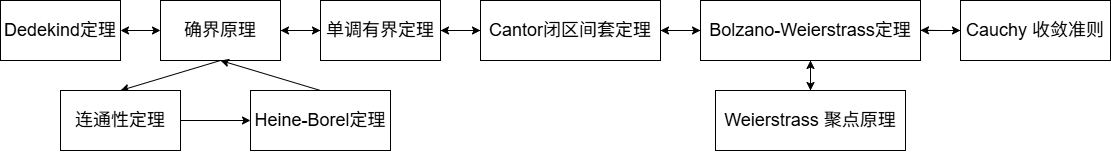
\includegraphics[width=1.0\linewidth]{figure/C2/111}
\end{center}
下面我们列举出其他的一些证明
\begin{proposition}
	用Cantor闭区间套定理证明确界原理
\end{proposition}
\begin{proof}
	
	设 $S$ 是非空有上界的实数集合，又设 $T$ 是由 $S$ 的所有上界所组成的集合，现证 $T$含有最小数，即 $S$ 有上确界．
	
	取 $a_1 \notin T, b_1 \in T$ ，显然 $a_1<b_1$ ．现按下述的规则依次构造一列闭区间：
	
	$$
	\begin{aligned}
		& {\left[a_2, b_2\right]= \begin{cases}{\left[a_1, \dfrac{a_1+b_1}{2}\right],} & \text { 若 } \dfrac{a_1+b_1}{2} \in T, \\
				{\left[\dfrac{a_1+b_1}{2}, b_1\right],} & \text { 若 } \dfrac{a_1+b_1}{2} \notin T ;\end{cases} } \\
		& {\left[a_3, b_3\right]= \begin{cases}{\left[a_2, \dfrac{a_2+b_2}{2}\right],} & \text { 若 } \dfrac{a_2+b_2}{2} \in T, \\
				{\left[\dfrac{a_2+b_2}{2}, b_2\right],} & \text { 若 } \dfrac{a_2+b_2}{2} \notin T ;\end{cases} }
	\end{aligned}
	$$
	
	$$\cdots$$
	
	由此得到一个闭区间套 $\left\{\left[a_n, b_n\right]\right\}$ ，满足
	
	$$
	a_n \notin  T, b_n \in T, \quad n=1,2,3, \cdots
	$$
	
	
	由闭区间套定理，存在惟一的实数 $\xi$ 属于所有的闭区间 $\left[a_n, b_n\right]$ ，且 $\lim\limits_{n \rightarrow \infty} a_n=\lim\limits _{n \rightarrow \infty} b_n=\xi$ ．现只需说明 $\xi$ 是集合 $T$ 的最小数，也就是集合 $S$ 的上确界．
	
	若 $\xi \notin T$ ，即 $\xi$ 不是集合 $S$ 的上界，则存在 $x \in S$ ，使得 $\xi<x$ ．由 $\lim\limits_{n \rightarrow \infty} b_n=\xi$ ，可知当 $n$ 充分大时，成立 $b_n<x$ ，这就与 $b_n \in T$ 发生矛盾，所以 $\xi \in T$ ．
	
	若存在 $\eta \in T$ ，使得 $\eta<\xi$ ，则由 $\lim\limits_{n \rightarrow \infty} a_n=\xi$ ，可知当 $n$ 充分大时，成立 $\eta<a_n$ ．由于 $a_n \in T$ ，于是存在 $y \in S$ ，使得 $\eta<a_n<y$ ，这就与 $\eta \in T$ 发生矛盾．从而得出 $\xi$ 是集合 $S$ 的上确界的结论．确界存在定理得证．
	
\end{proof}

\begin{proposition}
	确界原理证明有限覆盖定理
\end{proposition}

\begin{proof}
	构造集合 $S = \{x | a < x \leqslant b, [a, x]$ 能被 $H$ 中有限个开区间覆盖 $\}$；显然 $S$ 有上界,因 $H$ 覆盖闭区间 $[a, b]$,所以存在一个开区间 $(\alpha, \beta) \in H$ 使 $a \in (\alpha, \beta)$ .取 $x \in (\alpha, \beta)$ ,则 $[a, x]$ 能被 $H$ 中有限个开区间覆盖,从而 $x \in S$ ,故 $S$ 非空；

由确界原理存在 $\xi = \sup S$ ,现证 $\xi = b$ .用反证法.若 $\xi \neq b$ ,则 $a < \xi < b$ ,由 $H$ 覆盖闭区间 $[a, b]$,一定存在 $(\alpha_1, \beta_1) \in H$,使 $\xi \in (\alpha_1, \beta_1)$ .取 $x_1, x_2$ 使 $\alpha_1 < x_1 < \xi < x_2 < \beta_1$ ,且 $x_1 \in S$ ,则 $[a, x_1]$ 能被 $H$ 中有限个开区间覆盖,把 $(\alpha_1, \beta_1)$ 加进去,就推得 $x_2 \in S$ 这与 $\xi = \sup S$ 矛盾,故 $\xi = b$ ,即定理结论成立.
\end{proof}

\begin{proposition}
	确界原理证明$Cauchy$收敛准则
\end{proposition}
\begin{proof}
	必要性是由数列收敛定义直接得到的,不需要用到其它完备性定理.下面证充分性.（后面用其他定理证明$Cauchy$收敛准则都只证充分性,不再赘叙）
	
	设 $\{x_n\}$ 是$Cauchy$列,则 $\{x_n\}$ 是有界的（这一条也与其它实数完备性定理无关,后面用其他定理证明$Cauchy$收敛准则时直接使用,不再赘叙,请读者参考教材补充完整）.定义集合
	
	$$A = \{x | \text{存在正整数} N, \text{使任意的} n > N, \text{有} x_n > x\}  $$
	
	显然对于任意取定的 $\varepsilon > 0$ 和某个充分大的 $m$,必有 $x_m - \varepsilon \in A$,$x_m + \varepsilon \notin A$（否则将推出 $\{x_n\}$ 无界）,所以 $A$ 非空且有上界.由确界原理,$A$ 有上确界,记 $\sup A = a$.我们证明 $\{a_n\}$ 收敛于 $a$.
	
	任给 $\varepsilon > 0$,因为 $a$ 是 $A$ 的确界,故 $a - \varepsilon$ 必不是 $A$ 的上界,即存在 $x$ 属于 $A$,有 $x > a - \varepsilon$,由 $A$ 的定义知存在 $N$,使得对于任意 $n > N$,有 $x_n > a - \varepsilon$；又由$Cauchy$列的定义,存在 $N'$,使得对于任意的 $n, m > N'$,有 $|x_n - x_m| < \dfrac{\varepsilon}{2}$.显然 $a + \dfrac{\varepsilon}{2}$ 不属于 $A$,故对于 $N'$,必存在 $m' > N'$,且 $x_m \leqslant a + \dfrac{\varepsilon}{2}$,$|x_n - x_{m'}| < \dfrac{\varepsilon}{2}$,故 $x_n < a + \varepsilon$.于是任给 $\varepsilon > 0$,当 $n > \max\{N, N'\}$ 时,总有 $|x_n - a| < \varepsilon$,这就证明了$Cauchy$序列必定是收敛的.
\end{proof}
\begin{proposition}
	单调有界定理证明致密性定理
\end{proposition}
\begin{proof}
	
设 $S$ 是一有界无限点集,则在 $S$ 中可选取可数多个互不相同的点组成数列 $\{a_n\}$,显然数列 $\{a_n\}$ 是有界的.下面我们从 $\{a_n\}$ 中抽取一个单调子列,从而由单调有界定理该子列收敛,最后我们证明该子列的极限值,就是有界无限点集 $S$ 的聚点.

分两种情况来讨论：$(1)$ 如果在 $\{a_n\}$ 的任意一项之后,总存在最大的项,设 $a_1$ 后的最大项是 $a_{n_1}$,而 $a_{n_1}$ 后的最大项是 $a_{n_2}$,则显然 $a_{n_2} \leqslant a_{n_1}$.一般地,$a_{n_k}$ 后的最大项记为 $a_{n_{k+1}} (\leqslant a_{n_k}, k = 1, 2, \cdots)$.这样,就得到了 $\{a_n\}$ 的一个单调递减的子列 $\{a_{n_k}\}$,因为 $\{a_n\}$ 有界,由单调有界定理知,$\{a_{n_k}\}$ 收敛.

$(2)$. 如果 $(1)$ 不成立, 即从某一项以后, 任何一项都不是最大的, 由于前有限项不影响结果, 不妨设从第一项起, 每一项都不是最大项. 于是, 取 $a_{n_1} = a_1$ , 因 $a_{n_1}$ 不是最大项, 所以还存在另一项 $a_{n_2} > a_{n_1} (n_2 > n_1)$ , 又因为 $a_{n_2}$ 也不是最大项, 所以又有$a_{n_3} > a_{n_2} (n_3 > n_2)$ 这样一直作下去,就得到 $\{a_n\}$ 的一个单调递增子列 $\{a_{n_k}\}$,且这个子列有上界,由单调有界定理知,$\{a_{n_k}\}$ 收敛.

总之,不论 $\{a_n\}$ 属于情形 $(1)$ 还是情形 $(2)$,都可作出 $\{a_n\}$ 的一个单调收敛的子列.
\end{proof}




\begin{proposition}
	区间套定理证明确界原理
\end{proposition}

\begin{proof}
	只证明非空有上界的数集 $S$ 必有上确界,有下界的数集类似可证.

取 $S$ 的上界为 $b$ ,且 $b \notin S$ ；取 $a \in S$ ,且 $a$ 不是 $S$ 的上界,则 $a < b$ .

设闭区间 $[a_1, b_1] = [a, b]$. 

$Step\ 1$：取 $[a_1, b_1]$ 的中点 $\dfrac{a_1 + b_1}{2}$,若其是数集 $S$ 的上界,则取 $[a_2, b_2] = \left[a_1, \dfrac{a_1 + b_1}{2}\right]$；若不是数集 $S$ 的上界,则取 $[a_2, b_2] = \left[\dfrac{a_1 + b_1}{2}, b_1\right]$.

$Step\ 2$：取 $[a_2, b_2]$ 的中点 $\dfrac{a_2 + b_2}{2}$,若其是数集 $S$ 的上界,则取 $[a_3, b_3] = \left[a_2, \dfrac{a_2 + b_2}{2}\right]$；若不是数集 $S$ 的上界,则取 $[a_3, b_3] = \left[\dfrac{a_2 + b_2}{2}, b_2\right]$.

以此类推,

$Step\ n$：取 $[a_n, b_n]$ 的中点 $\dfrac{a_n + b_n}{2}$,若其是数集 $S$ 的上界,则取 $[a_{n+1}, b_{n+1}] = \left[a_n, \dfrac{a_n + b_n}{2}\right]$；若不是数集 $S$ 的上界,则取 $[a_{n+1}, b_{n+1}] = \left[\dfrac{a_n + b_n}{2}, b_n\right]$.

无限进行下去,易知

$$\lim\limits_{n \to \infty} (b_n - a_n) = \lim_{n \to \infty} \frac{b - a}{2^n} = 0. $$

(注意上述极限是$Archimedes$性质的一个等价命题) 则满足区间套定理,于是存在 $\xi \in \mathbb{R}$,有 $\xi \in \bigcap_{i=1}^{\infty} [a_i, b_i]$,且

$$\lim_{n \to \infty} b_n = \lim_{n \to \infty} a_n = \xi. $$

任取 $x \in S$ ,由二分法知 $x \leqslant b_n$ ,从而 $x \leqslant \lim\limits_{n \to \infty} b = \xi$ ,即 $\xi$ 是数集 $S$ 的一个上界.又由 $\lim\limits_{n \to \infty} a_n = \xi$ 知,$\forall \varepsilon > 0$,存在 $N$ ,当 $n > N$ 时,有 $a_n > \xi - \varepsilon$ .由分法知 $a_n$ 或者刚好是 $S$ 的上确界,或者不是 $S$ 的上界,则当 $n > N$ 时,存在 $x_0 \in S$ ,使得 $\xi - \varepsilon < a_n \leqslant x_0$.即 $\xi = \sup S$.
\end{proof}
\begin{proposition}
	区间套定理证明有限覆盖定理
\end{proposition}

\begin{proof}
	用反证法.假设定理的结论不成立,即不能用 $H$ 中有限个开区间来覆盖 $[a, b]$.

将 $[a, b]$ 等分为两个子区间,则其中至少有一个子区间不能用 $H$ 中有限个开区间来覆盖.记这个子区间为 $[a_1, b_1]$,则 $[a_1, b_1]\subset[a, b]$,且 $b_1-a_1=\dfrac{1}{2}(b-a)$.

再将 $[a_1, b_1]$ 等分为两个子区间,同样,其中至少有一个子区间不能用 $H$ 中有限个开区间来覆盖.记这个子区间为 $[a_2, b_2]$,则 $[a_2, b_2]\subset[a_1, b_1]$,且 $b_2-a_2=\dfrac{1}{2^2}(b-a)$.

重复上述步骤并不断地进行下去,则得到一个闭区间列 $\{[a_n, b_n]\}$,它满足

$$[a_n, b_n]\supset[a_{n+1}, b_{n+1}], n=1,2,\cdots, $$ $$b_n-a_n=\dfrac{b-a}{2^n}\to0(n\to\infty), $$

即 $\{[a_n, b_n]\}$ 是区间套,且其中每一个闭区间都不能用 $H$ 中有限个开区间来覆盖.

由区间套定理,存在唯一的一点 $\xi\in[a_n, b_n]$,$n=1,2,\cdots$.由于 $H$ 是 $[a, b]$ 的一个开覆盖,故存在开区间 $(\alpha, \beta)\in H$,使 $\xi\in(\alpha, \beta)$.于是,当 $n$ 充分大时有

$$[a_n, b_n]\subset(\alpha, \beta). $$

这表明 $[a_n, b_n]$ 只需用 $H$ 中的一个开区间 $(\alpha, \beta)$ 就能覆盖,与挑选 $[a_n, b_n]$ 时的假设“不能用 $H$ 中有限个开区间来覆盖”相矛盾.从而证得必存在属于 $H$ 的有限个开区间能覆盖$[a, b]$.

\end{proof}


\begin{proposition}
有限覆盖定理证明区间套定理
\end{proposition}

\begin{proof}
	反证法. 假设 $[a_n, b_n](n = 1, 2, \cdots)$ 没有公共点, 则 $[a_1, b_1]$ 上的任何一点都不是 $\{[a_n, b_n]\}$ 的公共点, 从而总存在一个开区间 $(x - \delta_x, x + \delta_x)$, 使得 $(x - \delta_x, x + \delta_x)$ 并非与所有的 $[a_n, b_n]$ 相交, 即存在 $[a_{n_x}, b_{n_x}]$, 使得 $[a_{n_x}, b_{n_x}]$ ∩ $(x - \delta_x, x + \delta_x) = \phi$.

现让 $x$ 取遍 $[a_1, b_1]$ 上的所有点就得到一个开区间集:

$$H = \{(x - \delta_x, x + \delta_x) | x \in [a_1, b_1]\}  $$

由有限覆盖定理, 可选出有限个开区间:

$$H' = \{(x_{k} - \delta_{x_k}, x_{k} + \delta_{x_k}) | k = 1, 2, \cdots, m\}  $$

覆盖闭区间 $[a, b]$, 其中

$$(x_{k} - \delta_{x_k}, x_{k} + \delta_{x_k}) \cap [a_{n_{x_k}}, b_{n_{x_k}}] = \phi  $$

因为 $[a_{n_{x_k}}, b_{n_{x_k}}]$ 只有有限个, 由区间套定理的条件, 它们是一个包含着一个, 因此其中一定有一个最小区间, 设为 $[a_{n_0}, b_{n_0}]$, 这时,

$$[a_{n_0}, b_{n_0}] \cap (x_{k} - \delta_{x_k}, x_{k} + \delta_{x_k}) = \phi, k = 1, 2, \cdots, m $$

从而,

$$[a_{n_0}, b_{n_0}] \cap \bigcup_{k=1}^{n} (x_{k} - \delta_{x_k}, x_{k} + \delta_{x_k}) = \phi $$

这就与 $[a_{n_0}, b_{n_0}] \subset [a_1, b_1]$ 矛盾. 所以 $[a_n, b_n](n = 1, 2, \cdots)$ 应有公共点.

\end{proof}
\begin{proposition}
	有限覆盖定理证明$Cauchy$收敛准则
\end{proposition}

\begin{proof}
	反证法.假设$Cauchy$列 ${x_n}$ 不收敛.已知 ${x_n}$ 为有界数列,而且 ${x_n}$ 是无穷点集（若 ${x_n}$ 是有限集,显然是收敛的）.

即存在闭区间 $[a, b]$ 使得 $\{x_n\} \subset [a, b]$. 则 $\forall x \in [a, b]$, $\exists U(x), \delta$ 使得 $U(x, \delta)$ 中只含有 $\{x_n\}$ 中的有限多项 (否则, 若 $\forall \delta > 0, U(x, \delta)$ 都有 $\{x_n\}$ 中的无限多项, 则易证 $\{x_n\}$ 收敛, 这与假设矛盾).

从而得 $[a, b]$ 的一个开覆盖 $H = \{U(x, \delta) | x \in [a, b]\}$, 由有限覆盖定理, 存在 $H$ 的一个有限子覆盖

$$H' = \{U(x_i, \delta_i) | x_i \in [a, b], i = 1, 2, \cdots, k\}, $$

所以 $\bigcup_{i=1}^{k} U(x_i, \delta_i)$ 只含有 $\{x_n\}$ 中的有限多个点, 这显然与 $\bigcup_{i=1}^{k} U(x_i, \delta_i) \supset [a, b] \supset \{x_n\}$ 矛盾. 因此 $\{x_n\}$ 必收敛.

\end{proof}


\begin{proposition}
	聚点定理证明确界原理
\end{proposition}

\begin{proof}
	设 $S$ 是非空有上界的数集.有限集时显然有上确界,不妨假设 $S$ 是无穷集合.

又设 $M$ 是 $S$ 的一个上界,如果 $M \in S$ 或者 $M$ 是 $S$ 的聚点（如果 $S$ 有聚点的话）,则 $M = \sup S$ ,定理成立.因此,下面假设 $M \in S$ 且 $M$ 不是 $S$ 的聚点.

在 $S$ 中任取一 $x_0$ ,总有 $x_0 < M$ ,考虑区间 $[x_0, M]$：

或者 $[x_0, M]$ 上只有 $S$ 的有限多个点,这时定理显然成立；或者 $[x_0, M]$ 上有 $S$ 的无穷多个点,那么, $S$ 在 $[x_0, M]$ 上的无穷多个点组成一有界的无穷点集.根据聚点原理, $S$ 在 $[x_0, M]$ 上必有聚点.

$(1)$ 若 $S$ 在 $[x_0, M]$ 上的聚点唯一,定理一定成立

事实上,若这个唯一聚点是 $x_0$ ,任取一个 $x_1 \in [x_0, M] \cap S$ ,则在 $[x_0, M]$ 上只能有 $S$ 的有限多个点（否则, $S$ 在 $[x_0, M]$ 上还有聚点,这与 $S$ 在 $[x_0, M]$ 上的聚点唯一相矛盾）,这时定理成立；

若这个唯一聚点是 $[x_0, M]$ 的内点 $\xi$ ,要么 $\xi$ 点的右边没有 $S$ 中的点,这时 $\xi = \sup S$ ,要么 $\xi$ 点右边还有 $S$ 中的点 $x_2$ ,那么在 $[x_2, M]$ 上只能有 $S$ 的有限多个点,其中最大者就是 $\sup S$ ,定理成立.

$(2)$ 若 $S$ 在 $(x_0, M)$ 上的聚点不是唯一的.

先证明下列结论成立：在 $(x_0, M)$ 内总存在一点 $x$ ,使得 $S$ 在 $[x, M]$ 上的聚点有且仅有一个.

假定这个结论不成立,那就是说对 $(x_0, M)$ 内的任意一点 $x$,或者在 $[x, M]$ 上总没有 $S$ 的聚点,或者在 $[x, M]$ 上总有 $S$ 的多个聚点.

如果前种情况发生,则根据 $x \in (x_0, M)$ 的任意性知 $(x_0, M)$ 内的任何内点都不是 $S$ 的聚点（因为假定有 $\xi \in [x_0, M]$ 是 $S$ 的聚点,则总有 $x_0 < x' < \xi < M$,于是 $[x', M]$ 上就有 $S$ 的聚点,这与在 $[x_0, M]$ 内的任意一点 $x$,$[x, M]$ 上总没有 $S$ 的聚点相矛盾）.与 $S$ 在 $(x_0, M)$ 上的聚点不是唯一的前提相矛盾.

如果后种情况发生,根据r的任意性推知$M$必是$S$的聚点,这又与前面“$M$不是$S$的聚点”的假设相矛盾.所以,上述结论必成立.

既然在 $(x_0, M)$ 内总存在一点 $x$,使得 $S$ 在 $[x, M]$ 上的聚点唯一,那么根据前面的讨论,定理成立.
\end{proof}

\begin{proposition}
	致密性定理证明有限覆盖定理
\end{proposition}

\begin{proof}
	设 $H$ 为 $[a, b]$ 的一个开覆盖,假设 $H$ 不存在有限子覆盖,则对 $[a, b]$ 二等分作区间套 $\{[a_n, b_n]\}$,使得每个 $[a_n, b_n]$ 都不存在有限子覆盖.

根据闭区间套的做法知,$\{b_n\}$ 为有界数列,故由致密性定理知,存在 $\{b_n\}$ 的子数列 $\{b_{n_k}\}$ 收敛,设 $\lim_{k \to \infty} b_{n_k} = \xi$,由 $\lim\limits_{k \to \infty} (b_{n_k} - a_{n_k}) = 0$ 知 $\lim\limits_{k \to \infty} a_{n_k} = \xi$,显然 $\xi \in [a, b]$.

由 $[a, b]$ 被 $H$ 覆盖知,存在开区间 $(\alpha, \beta) \in H$,使 $\xi \in (\alpha, \beta)$,由 $\lim_{k \to \infty} a_{n_k} = \lim\limits_{k \to \infty} b_{n_k} = \xi$ 知,存在充分大的 $K$ 使得 $[a_{n_K}, b_{n_K}] \subset (\alpha, \beta)$,这与 $[a_{n_K}, b_{n_K}]$ 不能被 $H$ 有限覆盖矛盾.故 $H$ 必有有限子覆盖.
\end{proof}


\begin{proposition}
	 $Cauchy$ 收敛准则证明单调有界定理
\end{proposition}

\begin{proof}
	设 $\{x_n\}$ 为递增有上界数列,下面我们用反证法证明数列 $\{x_n\}$ 有极限.假设 $\{x_n\}$ 不存在极限.由$Cauchy$ 收敛准则,$\exists \varepsilon_0 > 0, \forall N, \exists n > N$, 使得 $x_n - x_N = |x_n - x_N| > \varepsilon_0$.

依次取 $N_1 = 1, \exists n_1 > N_1$ 使得 $x_{n_1} - x_1 > \varepsilon_0$;

$$N_2 = n_1, \exists n_2 > n_1 \text{使得} x_{n_2} - x_{n_1} > \varepsilon_0; $$ $$\vdots $$ $$N_k = n_{k-1}, \exists n_k > n_{k-1} \text{使得} x_{n_k} - x_{n_{k-1}} > \varepsilon_0. $$

把以上式子相加得 $x_{n_k} - x_1 > k \varepsilon_0$,对任意的实数 $G$,当 $k > \dfrac{G - x_1}{\varepsilon_0}$ 时有 $x_{n_k} > G$,这与 $\{x_n\}$ 有上界矛盾.故数列 $\{x_n\}$ 有极限.

\end{proof}
\begin{proposition}
	$Cauchy$ 收敛准则证明致密性定理

\end{proposition}
\begin{proof}
	设 $S$ 是直线上的有界无限点集,所以 $\exists M > 0$,对任意的 $x \in S$ 都有 $-M \leqslant x \leqslant M$.

令 $[a_1, b_1] = [-M, M]$,则 $[a_1, b_1]$ 中含有 $S$ 的无穷多个点.

将 $[a_1, b_1]$ 二等分为两个小区间,则其中至少有一个闭区间含有 $S$ 的无穷多个点,记这样的小闭区间为 $[a_2, b_2]$.这样无限进行下去,得一闭区间套 $\{[a_n, b_n]\}$,每一个闭区间 $[a_n, b_n]$ 中都含有 $S$ 的无穷多个点.因此,存在 $x_1 \in S$ 使 $x_1 \in [a_1, b_1]$ ,存在 $x_2 \in S$ 使 $x_2 \in [a_2, b_2]$ 且 $x_2 \neq x_1$ ,一般地,存在 $x_n \in S$ 使 $x_n \in [a_n, b_n]$ 且 $x_n \notin {x_1, x_2, \cdots, x_{n-1}}$.

下面证明数列 $\{x_n\}$ 满足$Cauchy$收敛准则.

$\forall 0 < \varepsilon < 1$,取$N = \dfrac{\dfrac{\ln M}{\varepsilon}}{\ln 2}$,当 $m, n > N$ 时,有$x_m, x_n \in [a_{N+1}, b_{N+1}]$,则

$$|x_m - x_n| \leqslant b_{N+1} - a_{N+1} = \dfrac{M}{2^N} = \varepsilon  $$

故由$Cauchy$收敛准则知,数列 $\{x_n\}$ 收敛,设 $\lim\limits_{n \to \infty} x_n = \xi$.

\end{proof}










%

%% ===== 第一部分：单变量分析学 / 第4章：数列极限的应用与一些反例 =====
% !TEX root = ../../main.tex
\setchapterimage{figure/chapter4封面图.png}
\setchapterintro{本章的内容是对上一章数列部分的补充。}
\chapter{数列极限的应用与一些反例}
% 第1节：数列极限的定义与性质的应用
% !TEX root = ../../../main.tex
% 所属：第一部分：单变量分析学 / 第4章：数列极限的应用与一些反例
% 节：4.1 数列极限的定义与性质的应用
% 正文按原文件顺序保存；由 ../chapter4.tex 调用。
\section{数列极限的定义与性质的应用}
\begin{example}
	用极限定义证明 $\lim\limits _{n \rightarrow \infty} \dfrac{n}{n+3}=1$
	
\end{example}
\begin{proof}
	$\forall \varepsilon>0$ ，考虑
	
	$$
	\begin{aligned}
		& \left|\frac{n}{n+3}-1\right|<\varepsilon \\
		& \left|\frac{n}{n+3}-1\right|=\left|\frac{3}{n+3}\right|<\left|\frac{3}{n}\right|<\varepsilon
	\end{aligned}
	$$
	
	
	取 $N=\left[\dfrac{3}{\varepsilon}\right]+10$
	当 $n>N$ 时，必有 $\left|\dfrac{n}{n-3}-1\right|<\left|\dfrac{3}{n}\right|<\varepsilon$
\end{proof}
\begin{example}
	证明 $\left\{q^n\right\}, q \in(0,1)$ 是无穷小量
\end{example}
\begin{proof}
	$\forall \varepsilon>0$ ，考虑
	$$	\left|q^n\right|<\varepsilon $$
	取对数
	$$n \lg q<\lg \varepsilon$$
	
	
	取 $N=\left[\dfrac{\lg \varepsilon}{\lg q}\right]+10$
	
	$\forall n>N$ ，必有 $\left|q^n\right|<\varepsilon$
\end{proof}
\begin{proposition}\label{几个特殊的序列}
	几个特殊的序列
	\begin{enumerate}
		\item $a>0$ 时 $~\lim\limits _{n \rightarrow \infty} \dfrac{1}{n^a}=0$
		\item $a>0$时 $~\lim\limits _{n \rightarrow \infty} \sqrt[n]{a}=0$
		\item $\lim\limits _{n \rightarrow \infty} \sqrt[n]{n}=1$
		更一般地 $\forall k \in \mathbb{Z}_{+}$
		
		$$
		\lim _{n \rightarrow \infty} \sqrt[n]{n^k}=1
		$$
		\item $p>0$ ,而 $\alpha \in \mathbb{R}$
		
		$$
		\lim _{n \rightarrow \infty} \frac{n^\alpha}{(1+p)^n}=0
		$$
	\end{enumerate}
	
\end{proposition}
\begin{proof}
	（1）$\forall \varepsilon>0~$ ,考虑 $~\left|\dfrac{1}{(n)^{\alpha}}\right|<\varepsilon$
	取 $N=\left[\left(\dfrac{1}{\varepsilon}\right)^{1 / \alpha}\right]+1 $,$~ \forall n \rightarrow N$ 即可
	
	(2) $a>1 ~$ 时, 令$~y_n= \sqrt[n]{a}-1~,$那么 
	
	$$
	\begin{aligned}
		a=\left(1+y_n\right)^n&=1+n y_n+\cdots \\
		&>1+n y_n
	\end{aligned}
	$$
	
	
	也即
	
	$$
	y_n=\sqrt[n]{a}-1<\frac{a-1}{n}
	$$
	
	$\forall \varepsilon>0$ ，考虑 $$|\sqrt[n]{a}-1|<\frac{a-1}{n}<\varepsilon$$
	取 $~N=\left[\dfrac{a-1}{\varepsilon}\right]+10 ~$，则$~ \forall n >N$ 时
	
	$$
	|\sqrt[n]{a}-1|<\varepsilon
	$$
	
	$0<a<1$ 时 $\left(\dfrac{1}{a}\right)^{1 / n} \rightarrow 1$ 故 $(a)^{1 / n} \rightarrow 1$
	
	$a=1$ 时 ,显然
	
	（3）令$\sqrt[n]{n}-1=y_n$, 那么
	
	$$
	n=\left(1+y_n\right)^n=1+n y_n+\dfrac{n(n-1)}{2} y_n^2+\cdots 
	>\dfrac{n(n-1)}{2} y_n^2$$
	
	
	也即
	
	$$
	y_n<\sqrt{\dfrac{2}{n-1}}<\varepsilon
	$$
	
	
	取 $N=\left[\dfrac{2}{\varepsilon^2}+1\right]+10, ~~ \forall n>N$ 时
	
	$$
	|\sqrt[n]{n}-1|<\varepsilon
	$$
	
	
	对 $\lim\limits_{n \rightarrow \infty} \sqrt[n]{n^k}=1$ ，利用极限的乘法即可
	
	（4）设 $k \in \mathbb{Z}_{+}, ~ k > \alpha$ ，当 $n>k$ 时
	
	$$
	(1+p)^n>C_n^k p^k>\dfrac{n^k p^k}{k!} .
	$$
	
	
	从而 $\quad 0<\dfrac{n^\alpha}{(1+p)^n}<\dfrac{k!}{p^k} n^{\alpha-k}$
	且 $\alpha-k<0 ~$ 由（1）$~ n^{\alpha-k} \rightarrow 0$
	
	由夹逼性 $$\quad \lim _{n \rightarrow \infty} \dfrac{n^\alpha}{(1+p)^n}=0$$
	
\end{proof}
\begin{example}
	已知 $\lim\limits_{n \to \infty} a_n = a$，证明：
	$$\lim\limits_{n\to\infty}\dfrac{1}{2^n}\sum_{k=0}^{n}{n \choose k}a_k=a$$
	
\end{example}
\begin{proof}
	
	$$ \left| \dfrac{1}{2^n} \sum_{k=0}^{n} {n \choose k} a_k - a \right| = \left| \dfrac{1}{2^n} \sum_{k=0}^{n} {n \choose k} (a_k - a) \right| \leqslant \dfrac{1}{2^n} \sum_{k=0}^{n} {n \choose k} |a_k - a| $$
	$\forall \varepsilon > 0, \exists N_1 \text{ 使得当 } k > N_1 \text{ 时 }, |a_k - a| < \varepsilon$, 对所有的 $k$ 成立.
	
	\begin{align*}
		\frac{1}{2^n} \sum_{k=0}^{n} {n \choose k} |a_k - a| &= \frac{1}{2^n} \sum_{k=0}^{N_1} {n \choose k} |a_k - a| + \frac{1}{2^n} \sum_{k=N_1+1}^{n} {n \choose k} |a_k - a| \\
		&< \frac{1}{2^n} \sum_{k=0}^{N_1} {n \choose k} |a_k - a| + \varepsilon \\
		&< \frac{M (1 + n + \cdots + n^{N_1})}{2^n} + \varepsilon
	\end{align*}
	
	当 $n \to \infty$ 时, $\dfrac{1 + n + \cdots + n^{N_1}}{2^n} \to 0$，$M$ 是 $|a_k - a|$ 在 $N_1$ 内的上界.
	
	取 $N_2$,对所有 $n > N_2$,都有
	
	$$ \frac{M (1 + n + \cdots + n^{N_1})}{2^n} < \varepsilon $$
	
	取 $n > \max\{N_1, N_2\}$,就有
	
	$$ \left| \frac{1}{2^n} \sum_{k=0}^{n} {n \choose k} a_k - a \right| < 2\varepsilon $$
	
\end{proof}







\begin{proposition}(Cesaro平均定理)
	若$\lim\limits_{n\to\infty}a_n=a,$那么
	$$\lim\limits_{n\to\infty}\frac{a_1+\cdots+a_n}{n}=a$$
	\label{Cesaro}
\end{proposition}
\begin{proof}
	假设$a=0$,$\forall\varepsilon>0,\exists N_1\in \Z_{+},\forall n>N_1$,有$|a_n|<\varepsilon$
	$$\begin{aligned}
		\left|\frac{a_1+\cdots+a_n}{n}\right| & =\left|\frac{a_1+\cdots+a_{N_1}}{n}+\frac{a_{N_1+1}+\cdots+a_n}{n}\right| \\
		& \leqslant\left|\frac{a_1+\cdots+a_{N_1}}{n}\right|+\left|\frac{a_{N_1+1}+\cdots+a_n}{n}\right| \\
		& <\left|\frac{a_1+\cdots+a_{N_1}}{n}\right|+\varepsilon
	\end{aligned}$$
	对于固定的 $\varepsilon, N_1,\left|\dfrac{a_1+\cdots+a_{N_1}}{n}\right|$ 是固定的
	
	设 $c=a_1+\cdots+a_{N_1}$ ,想使 $\left|\dfrac{c}{n}\right|$ 与 $\varepsilon$ 有关,使 $\left|\dfrac{c}{n}\right|<\varepsilon$ ,取 $N_2=\left[\dfrac{c}{\varepsilon}\right]+100 n>N_2$ 时，$\left|\dfrac{c}{n}\right|<\varepsilon$
	
	$\forall n>\max \left[N_1, N_2\right] ~,~\left|\dfrac{a_1+\cdots+a_n}{n}\right|<\varepsilon+\varepsilon=2 \varepsilon$,即
	
	
	$$\lim _{n \rightarrow \infty} \frac{a_{1}+\cdots+a_n}{n}=a$$
	
\end{proof}
\begin{corollary}
	已知 $\lim\limits_{n \to \infty} a_n = a$，证明：
	
	$$ \lim_{n \to \infty} \sqrt[n]{a_1 \cdots a_n} = a $$
	\label{cesaro's co}
\end{corollary}
\begin{proof}
	设 $a_n > 0$ 且 $a > 0$（否则结论需要单独处理）. 由 $\lim\limits_{n \to \infty} a_n = a$ 和命题\ref{Cesaro}，有
	
	$$ \lim_{n \to \infty} \dfrac{\dfrac{1}{a_1} + \cdots + \dfrac{1}{a_n}}{n} = \dfrac{1}{a} $$
	
	因此
	
	$$ \lim_{n \to \infty} \dfrac{n}{\dfrac{1}{a_1} + \cdots + \dfrac{1}{a_n}} = a $$
	
	由基本不等式
	
	$$ \lim_{n \to \infty} \sqrt[n]{a_1 \cdots a_n} = a $$
	
	
\end{proof}
命题\ref{Cesaro}与命题\ref{cesaro's co}在下一节中将使用Stolz定理证明.

\begin{example}
	
	$a_i \geqslant 0$，证明：
	
	$$ \lim_{n \to \infty} (a_1^n + \cdots + a_p^n)^{1/n} = \max \{a_i\} $$
	
	
	
\end{example}
\begin{proof}
	由算术几何平均不等式,
	
	$$ \max \{a_i\} \leqslant (a_1^n + \cdots + a_p^n)^{1/n} \leqslant \max \{a_i\} \cdot p^{1/n} $$
	
	对于 $p \geqslant 1$,由夹逼性,得证.
\end{proof}
\begin{example}
	关于极限定义的一些反例:
	
	(1) $\forall \varepsilon > 0, \exists N$, 使得 $\forall n > N$，$x_n < \varepsilon$.
	
	取 $x_n = -n$，$N = 1$，$x_1, \ldots, x_n, \ldots < 0 < \varepsilon$.
	
	(2) $\forall \varepsilon > 0$，无穷多 $x_n$，$x_n < \varepsilon$.
	
	取 $x_n = (-1)^n$.
\end{example}

\begin{proposition}
	$\forall k \in \mathbb{Z}^+$，
	
	$$ \lim_{n \to \infty} x_n = a \Leftrightarrow \lim_{n \to \infty} x_{n+k} = a $$
\end{proposition}
\begin{proof}
	$\Rightarrow$: $\forall \varepsilon > 0, \exists N, \forall n > N$, 有 $|x_n - a| < \varepsilon$.
	
	对于 $n + k > N$，有 $|x_{n+k} - a| < \varepsilon$.
	
	因此，
	$$ \lim_{n \to \infty} x_{n+k} = a $$
	
	$\Leftarrow$: $\forall \varepsilon > 0, \exists N, \forall n + k > N$, 有 $|x_{n+k} - a| < \varepsilon$.
	
	对于 $n > N + k$，有 $|x_n - a| < \varepsilon$.
	
	因此，
	
	$$ \lim_{n \to \infty} x_n = a $$
\end{proof}
\begin{example}
	对于任意 $|q| > 0$，记明 $\left\{q^n\right\}$ 是无穷大量.
	
\end{example}
\begin{proof}
	$\forall G> 1$，考虑 $q^n > G$.
	
	取 $N = \left\lfloor \dfrac{\lg G}{\lg q} \right\rfloor + 1$，则对于 $\forall n > N$，成立
	$$ q^n > G$$
\end{proof}
\begin{example}
	$x_n \neq 0$，$\{x_n\}$ 是无穷大量当且仅当 $\{\dfrac{1}{x_n}\}$ 是无穷小量
\end{example}
\begin{proof}
	若 $\{x_n\}$ 是无穷大量，取 $G = \dfrac{1}{\varepsilon}$，
	
	$\forall G > 0, \exists N, \forall n > N$ 时，$|x_n| > G= \dfrac{1}{\varepsilon} \Leftrightarrow |x_n| > \dfrac{1}{\varepsilon} \Leftrightarrow \left|\dfrac{1}{x_n}\right| < \varepsilon$，即 $\left\{\dfrac{1}{x_n}\right\}$ 是无穷小量.
	
	若 $\left\{\dfrac{1}{x_n}\right\}$ 是无穷小量，取 $\varepsilon = \dfrac{1}{G}$，
	
	$\forall G > 0, \exists N, \forall n > N$ 时，$\left|\dfrac{1}{x_n}\right| < \varepsilon = \dfrac{1}{G} \Leftrightarrow |x_n| > G$，即 $\{x_n\}$ 是无穷大量.
\end{proof}


%
% 第2节：Stolz定理及其应用
% !TEX root = ../../../main.tex
% 所属：第一部分：单变量分析学 / 第4章：数列极限的应用与一些反例
% 节：4.2 Stolz定理及其应用
% 正文按原文件顺序保存；由 ../chapter4.tex 调用。
\section{Stolz定理及其应用}
在进行极限的计算时,我们发现了$\dfrac{*}{\infty},\dfrac{0}{0}$的情况,我们称之为待定型，下面给出一种解决的方案——Stolz定理
\begin{theorem}
	设 $\{y_n\}$ 是严格单调递增的正无穷大量，且
	
	$$ \lim_{n \to \infty} \dfrac{x_n - x_{n-1}}{y_n - y_{n-1}} = a \quad (a \in \mathbb{R}^* ) $$
	
	则
	
	$$ \lim_{n \to \infty} \frac{x_n}{y_n} = a $$
	
\end{theorem}
\begin{proof}
	首先考虑 $a = 0$.由 $\lim\limits_{n \to \infty} \dfrac{x_n - x_{n-1}}{y_n - y_{n-1}} = 0$，对于 $\forall \varepsilon > 0, \exists N_1, \forall n > N_1$，
	
	$$ |x_n - x_{n-1}| < \varepsilon (y_n - y_{n-1} ) $$
	
	由于 $\{y_n\}$ 是严格单调递增的正无穷大量，显然，可以取 $y_{N_1} > 0$，于是
	\begin{align*}
		|x_n - x_{N_1}| & \leqslant |x_n - x_{n-1}| + \cdots + |x_{N_1+1} - x_{N_1}| \\
		& < \varepsilon (y_n - y_{n-1}) + \cdots + \varepsilon (y_{N_1+1} - y_{N_1}) \\
		& = \varepsilon (y_n - y_{N_1})
	\end{align*}
	
	因此，
	
	$$ \left| \frac{x_n}{y_n} - \frac{x_{N_1}}{y_n} \right| \leqslant \varepsilon \left(1 - \frac{y_{N_1}}{y_n}\right) < \varepsilon $$
	
	对于固定的 $N_1$，再取 $N > N_1$，使得 $\forall n > N$，有 $\left| \dfrac{x_{N_1}}{y_n} \right| < \varepsilon$，从而
	
	$$ \left| \frac{x_n}{y_n} \right| <\varepsilon+ \left| \frac{x_{N_1}}{y_n} \right| <  2\varepsilon $$
	
	当 $a$ 是有限非零实数时，令 $x_n' = x_n - a y_n$，则有
	
	$$ \lim_{n \to \infty} \frac{x_n' - x_{n-1}'}{y_n - y_{n-1}} = \lim_{n \to \infty} \frac{x_n - x_{n-1} }{y_n - y_{n-1}} - a= 0 $$
	
	得到
	
	$$ \lim_{n \to \infty} \frac{x_n'}{y_n} = 0 $$
	
	从而
	
	$$ \lim_{n \to \infty} \frac{x_n}{y_n} = \lim_{n \to \infty} \frac{x_n'}{y_n} + a = a $$
	
	对于 $a = +\infty$ 的情况：$\exists N, \forall n > N$，
	
	$$ x_n - x_{n-1} > y_n - y_{n-1} $$
	
	这说明 $\{x_n\}$ 也严格单调递增，且从 $x_n - x_{n-1} > y_n - y_{n-1}$ 知
	\[
	x_n - x_N > y_n - y_N \quad (n > N).
	\]
	由于 $\{y_n\}$ 是正无穷大量，$y_n - y_N \to +\infty$，故 $x_n \to +\infty$.
	又由 $x_n - x_{n-1} > y_n - y_{n-1} > 0$ 对 $n > N$ 成立，有
	\[
	\frac{y_n - y_{n-1}}{x_n - x_{n-1}} \to 0 \quad (n\to\infty).
	\]
	现对 $\left\{\dfrac{y_n}{x_n}\right\}$ 应用已证的 $a=0$ 情形（注意 $\{x_n\}$ 严格递增且趋于 $+\infty$）：
	\[
	\lim_{n \to +\infty} \frac{y_n}{x_n}
	= \lim_{n \to +\infty} \frac{y_n - y_{n-1}}{x_n - x_{n-1}} = 0.
	\]
	从而
	\[
	\lim_{n \to +\infty} \frac{x_n}{y_n} = +\infty.
	\]
	
	对于 $a = -\infty$ 的情况，类似
\end{proof}
\begin{theorem}
	设 $\{a_n\}$ 和 $\{b_n\}$ 都是无穷小量，且 $\{a_n\}$ 是严格单调递减，又有
	
	$$ \lim_{n \to \infty} \frac{b_{n+1} - b_n}{a_{n+1} - a_n} = l \quad (l \in\R^*) $$
	
	则有
	
	$$ \lim_{n \to \infty} \frac{b_n}{a_n} = l $$
\end{theorem}
\begin{proof}
	记 $l \neq\pm \infty$，
	
	$\forall \varepsilon > 0, \exists N, \forall n > N$，有
	
	$$ \left| \frac{b_{n+1} - b_n}{a_{n+1} - a_n} - l \right| < \varepsilon $$
	
	由 $\{a_n\}$ 单调性，
	
	$$ (l - \varepsilon)( a_n-a_{n+1} ) <  b_n-b_{n+1}  < (l + \varepsilon)( a_n- a_{n+1}) $$
	
	任取 $m > n$，
	$$\begin{aligned}
		&(l - \varepsilon)( a_n-a_{n+1} ) <  b_n-b_{n+1}  < (l + \varepsilon)( a_n- a_{n+1})\\
		&(l - \varepsilon)(a_{n+1} - a_{n+2}) < b_{n+1} - b_{n+2} < (l + \varepsilon)(a_{n+1} - a_{n+2})\\
		&\vdots\\
		&(l - \varepsilon)(a_{m-1} - a_{m}) < b_{m-1} - b_{m} < (l + \varepsilon)(a_{m-1} - a_{m})
	\end{aligned}$$
	
	
	累加得
	
	$$ (l - \varepsilon)(a_n - a_m) < b_n - b_m < (l + \varepsilon)(a_n - a_m) $$
	
	因此
	
	$$ \left| \frac{b_n - b_m}{a_n - a_m} - l \right| < \varepsilon $$
	
	当 $m \to +\infty$，$\lim\limits_{m \to \infty} a_m = \lim\limits_{m \to \infty} b_m = 0$，故 $\forall n> N$，
	
	$$ \left| \frac{b_n}{a_n} - l \right| < \varepsilon $$
	
	对于 $l = +\infty$ 的情况，$\forall G, \exists N, \forall n > N$ 都有
	
	$$ \frac{b_n - b_{n+1}}{a_n - a_{n+1}} > G $$
	
	即
	
	$$ b_n - b_{n+1} > G (a_n - a_{n+1}) $$
	
	任取 $m > n$，
	$$\begin{aligned}
		&b_{n+1} - b_{n+2} > G (a_{n+1} - a_{n+2})\\
		&\vdots\\
		&b_{m-1} - b_{m} > G (a_{m-1} - a_{m})
	\end{aligned}$$
	
	
	累加得
	
	$$ b_n - b_m > G (a_n - a_m) $$
	
	当 $m \to +\infty$，
	
	$$ \frac{b_n}{a_n} > G $$
	
	也即
	
	$$ \lim_{n \to \infty} \frac{b_n}{a_n} = +\infty $$
	
	对于 $l = -\infty$ 的情况类似
\end{proof}

\begin{example}
	证明
	$$ \lim_{n \to \infty} \dfrac{1^k + 2^k + \cdots + n^k}{n^{k+1}}= \dfrac{1}{k+1} $$
	
\end{example}
\begin{proof}
	设 $x_n = 1^k + \cdots + n^k$，$y_n = n^{k+1}$，且 $y_n $严格单调上升至正无穷，
	
	$$ \lim_{n \to \infty} \frac{x_n - x_{n-1}}{y_n - y_{n-1}} = \lim_{n \to \infty} \frac{n^k}{n^{k+1} - (n-1)^{k+1}} = \frac{1}{k+1} $$
	
	由 Stolz 定理，
	
	$$ \lim_{n \to \infty} \frac{x_n}{y_n} = \frac{1}{k+1} $$
\end{proof}
注意此处的逻辑顺序是先有$\lim\limits_{n \to \infty} \dfrac{x_n - x_{n-1}}{y_n - y_{n-1}}$,再有$\lim\limits_{n \to \infty}\dfrac{x_n}{y_n}$.
\begin{corollary}
	若 $\lim\limits_{n \to \infty} a_n = a$，则
	
	(1)
	$$ \lim_{n \to \infty} \frac{a_1 + \cdots + a_n}{n} = a $$
	
	(2)若 $\lim\limits_{n \to \infty} (x_{n+1} - x_n) = a$，则
	$$ \lim_{n \to \infty} \frac{x_n}{n} = a $$
	
	(3) 若$a>0$,则$$\lim\limits_{n\to\infty}\sqrt[n]{a_1\cdots a_1}=a$$
	
	(4) 若 $\lim\limits_{n \to \infty} \dfrac{x_{n+1}}{x_n} = a$，则
	$$ \lim_{n \to \infty} \sqrt[n]{x_n} = a $$
	\label{imcoofstolz}
\end{corollary}
\begin{proof}
	(1) 
	\[
	\lim_{n \to \infty} a_n = \lim_{n \to \infty} \frac{(a_1 + \cdots + a_n) - (a_1 + \cdots + a_{n-1})}{n - (n-1)} = \lim_{n \to \infty} \frac{a_1 + \cdots + a_n}{n} = a
	\]
	
	(2) \[
	\lim_{n \to \infty} \frac{x_n}{n} = \lim_{n \to \infty} \left[ \frac{x_n - x_{n+1} + \cdots + x_2 - x_1}{n} + \frac{x_1}{n} \right] = \lim_{n \to \infty} (x_{n+1} - x_n) + \lim_{n \to \infty} \frac{x_1}{n} = a
	\]
	
	(3)由基本不等式，
	\[
	\dfrac{n}{\dfrac{1}{a_1} + \cdots + \dfrac{1}{a_n}} \leqslant \sqrt[n]{a_1 \cdots a_n} \leqslant \dfrac{a_1 + \cdots + a_n}{n}
	\]
	由夹逼定理，
	\[
	\lim_{n \to \infty} \sqrt[n]{a_1 \cdots a_n} = a
	\]
	
	
	(4)\[
	\lim_{n \to \infty} \sqrt[n]{x_1 \cdot \frac{x_2}{x_1} \cdot \frac{x_3}{x_2} \cdots \frac{x_n}{x_{n-1}}} = \lim_{n \to \infty} \frac{x_{n+1}}{x_n} = a
	\]
	
\end{proof}


\begin{example}
	(1)
	$$ \lim_{n \to \infty} \frac{1}{\sqrt[n]{n!}} = 0 $$
	
	(2)
	$$ \lim_{n \to \infty} \frac{n}{\sqrt[n]{n!}} = e $$
	
	(3) 若 $\lim\limits_{n \to \infty} (x_{n+2} - x_n) = a$，则
	$$ \lim_{n \to \infty} \frac{x_n}{n} = \frac{a}{2} $$
	
	(4) $\lim\limits_{n \to \infty} x_{2n} = a$，$\lim\limits_{n \to \infty} x_{2n+1} = b$，证明
	$$ \lim_{n \to \infty} \frac{x_1 + \cdots + x_n}{n} = \frac{a + b}{2} $$
\end{example}
\begin{proof}
	(1) 设 $x_n = \dfrac{1}{n!}$，证明 $\dfrac{x_{n+1}}{x_n} = \dfrac{1}{n+1}$，由\ref{imcoofstolz}(3)，$\lim\limits_{n \to \infty} \dfrac{x_{n+1}}{x_n} = 0$，
	
	得
	\[
	\lim_{n \to \infty} \frac{1}{ \sqrt[n]{n!}} = \lim_{n \to \infty} \sqrt[n]{x_n} = 0
	\]
	
	(2) 设 $x_n = \dfrac{n^n}{n!}$，证明 $\dfrac{x_{n+1}}{x_n} = \left(1 + \dfrac{1}{n}\right)^n$，由 $\lim\limits_{n \to \infty} \left(1 + \dfrac{1}{n}\right)^n = e$(由第4节)，
	
	\[
	\lim_{n \to \infty} \frac{n}{\sqrt[n]{n!}} = \lim_{n \to \infty}  \sqrt[n]{x_n} = e
	\]
	
	(3) 对偶数项 $\left\{ \dfrac{x_{2n}}{2n} \right\}$，
	由 $\lim\limits_{n \to \infty} (x_{2n+2} - x_{2n}) = a$，由 \ref{imcoofstolz}(4) 得 $\lim\limits_{n \to \infty} \dfrac{x_{2n}}{n} = a$，
	也即 $\lim\limits_{n \to \infty} \dfrac{x_{2n}}{2n} = \dfrac{a}{2}$.
	
	对奇数项 $\left\{ \dfrac{x_{2n-1}}{2n-1} \right\}$，
	由 $\lim\limits_{n \to \infty} (x_{2n+1} - x_{2n-1}) = a$，由 \ref{imcoofstolz}(4)得 $\lim\limits_{n \to \infty} \dfrac{x_{2n-1}}{n} = a$，
	也即 $\lim\limits_{n \to \infty} \dfrac{x_{2n-1}}{2n-1} \cdot \dfrac{2n-1}{2n} = \dfrac{a}{2}$.
	
	由 \ref{oddandeven}，
	\[
	\lim_{n \to \infty} \frac{x_n}{n} = \frac{a}{2}
	\]
	(4) 对 $\left\{ \dfrac{x_1 + \cdots + x_n}{n} \right\}$ 的偶子列，
	\[
	\lim_{n \to \infty} \frac{x_1 + \cdots + x_{2n}}{2n} = \lim_{n \to \infty} \left( \frac{x_1 + x_3 + \cdots + x_{2n-1}}{2n} + \frac{x_2 + \cdots + x_{2n}}{2n} \right)
	\]
	\[
	= \lim_{n \to \infty} \frac{x_{2n-1}}{2} + \lim_{n \to \infty} \frac{x_{2n}}{2} = \frac{a + b}{2}
	\]
	
	对奇子列，
	\[
	\lim_{n \to \infty} \frac{x_1 + \cdots + x_{2n+1}}{2n+1} = \lim_{n \to \infty} \left( \frac{x_1 + x_3 + \cdots + x_{2n+1}}{n+1} \cdot \frac{n+1}{2n+1} + \frac{x_2 + \cdots + x_{2n}}{2n+1} \cdot \frac{n}{2n+1} \right)
	\]
	\[
	= \lim_{n \to \infty} \frac{x_{2n+1}}{2} + \lim_{n \to \infty} \frac{x_{2n}}{2} = \frac{a + b}{2}
	\]
	
	对(4) 我们做下列的推广，若
	\[
	\lim_{n \to \infty} x_{kn+i} = m_i \quad i = 0, 1, \ldots, k-1
	\]
	
	则
	\[
	\lim_{n \to \infty} \frac{x_1 + \cdots + x_n}{n} = \frac{m_1 + \cdots + m_k}{k}
	\]
	
\end{proof}
\begin{example}
	已知 $\lim\limits_{n \to \infty} a_n = a$，$\lim\limits_{n \to \infty} b_n = b$，证明
	\[
	\lim_{n \to \infty} \dfrac{a_1 b_n + \cdots + a_n b_1}{n} = ab
	\]
\end{example}
\begin{proof}
	考虑 $$\left| \dfrac{a_1 b_n + \cdots + a_n b_1}{n} - ab \right| = \left| \frac{(a_1 b_n - ab) + \cdots + (a_n b_1 - ab)}{n} \right|$$
	设 $M$ 为 $|a_n|$ 的界，也即 $|a_n| \leqslant M$，
	\[
	|a_1 b_n - ab| = |a_1 b_n - a_1 b + a_1 b - ab| \leqslant |a_1||b_n - b| + |b||a_1 - a| \leqslant M |b_n - b| + b |a_1 - a|
	\]
	$$\begin{aligned}
		\left| \frac{(a_1 b_n - ab) + \cdots + (a_n b_1 - ab)}{n} \right| &\leqslant \frac{M |b_n - b| + \cdots + M |b_n - b|}{n} + \frac{b |a_1 - a| + \cdots + b |a_n - a|}{n}\\&\to 0 + 0 = 0
	\end{aligned}$$
\end{proof}
\begin{proposition} (Abel 变换)
	对于数列 $\{a_n\}, \{b_i\}$，定义 $A_k = \sum\limits_{n=1}^k a_n$，则有：
	
	\[
	\sum_{i=1}^n a_i b_i = b_n A_n + \sum_{i=1}^{n-1} A_i (b_i - b_{i+1})
	\]
	\label{Abeltra}
\end{proposition}
\begin{proof}
	\begin{align*}
		\sum_{i=1}^n a_i b_i &= \sum_{i=1}^n (A_i - A_{i-1}) b_i \\
		&= A_1 b_1 + (A_2 - A_1) b_2 + \cdots + (A_n - A_{n-1}) b_n \\
		&= A_1 b_1 + A_2 (b_2 - b_3) + \cdots + A_n b_n - A_{n-1} b_n \\
		&= b_n A_n + \sum_{i=1}^{n-1} A_i (b_i - b_{i+1})
	\end{align*}
	
\end{proof}
\begin{example}
	
	若 $A_n = \sum\limits_{k=1}^n a_k$ 收敛于 $A$，证明：
	
	(1)
	\[
	\lim_{n \to \infty} \frac{a_1 + 2a_2 + \cdots + n a_n}{n} = 0
	\]
	
	(2) 若 $a_n>0$，则
	\[
	\lim_{n \to \infty} \sqrt[n]{n!a_1 \cdots a_n} = 0
	\]
	
	(3) 若 $\{p_n\}$ 严格递增且 趋近于$ +\infty$，则
	\[
	\lim_{n \to \infty} \frac{a_1 p_1 + \cdots + a_n p_n}{p_n} = 0
	\]
	
\end{example}



\begin{proof}
	考虑(3)即可
	
	由\ref{Abeltra} Abel 变换，
	\[
	a_1 p_1 + \cdots + a_n p_n = p_n A_n + \sum_{k=1}^{n-1} A_k (p_k - p_{k+1})
	\]
	
	因为 $A_n \to A$，且 $p_n \to +\infty$，所以
	
	$$\begin{aligned}
		\lim_{n \to \infty} \frac{a_1 p_1 + \cdots + a_n p_n}{p_n}& = 	\lim_{n \to \infty}\left[A_n + \frac{1}{p_n} \sum_{k=1}^{n-1} A_k (p_k - p_{k+1})\right]\\&=\lim\limits_{n\to \infty}A_n+\lim\limits_{n\to \infty}\frac{A_{n-1}(p_{n-1}-p_{n})}{p_{n}-p_{n-1}}=A-A = 0
	\end{aligned}$$
	
	
	
\end{proof}

%
% 第3节：单调有界收敛原理的应用
% !TEX root = ../../../main.tex
% 所属：第一部分：单变量分析学 / 第4章：数列极限的应用与一些反例
% 节：4.3 单调有界收敛原理的应用
% 正文按原文件顺序保存；由 ../chapter4.tex 调用。
\section{单调有界收敛原理的应用}
\begin{example}
	利用单调有界收敛原理，证明 $\left\{\dfrac{n^5}{2^n}\right\}$ 收敛.
	
	
\end{example}
\begin{proof}
	设 $a_n = \dfrac{n^5}{2^n}$，那么
	
	\[
	\frac{a_{n+1}}{a_n} = \frac{1}{2} \left(1 + \frac{1}{n}\right)^5
	\]
	
	对于 $(1 + \dfrac{1}{n})^5$，$\exists N$，当 $n > N$ 时，$(1 + \dfrac{1}{n})^5 < 2$.因此 $\forall n > N$，
	
	\[
	a_{n+1} = \frac{1}{2} \left(1 + \frac{1}{n}\right)^5 a_n < a_n
	\]
	
	从 $n > N$ 起 $\{a_n\}$ 单调递减，且 $a_n \geqslant 0$，所以 $\exists a\in\R$使得$a = \lim\limits_{n\to\infty} a_n$，
	
	\[
	\lim_{n \to \infty} a_{n+1} = \lim_{n \to \infty} \frac{1}{2} \left(1 + \frac{1}{n}\right)^5 a_n = a
	\]
	
	\[
	a = \frac{1}{2} a \implies a = 0
	\]
\end{proof}

\begin{example}
	设 $x_1 > 0$，$x_{n+1} = 1 + \dfrac{x_n}{1 + x_n}$，$n = 1, 2, 3, \dots$
	
	证明 $\{x_n\}$ 收敛，并求极限值.
\end{example}
\begin{proof}
	观察 $x_{n+1} = 1 + \dfrac{x_n}{1 + x_n}$，注意到 $\dfrac{x_n}{1 + x_n} < 1$，所以 $x_{n+1} < 2$.
	
	
	$n = 2$ 时，$x_2 = 1 + \dfrac{x_1}{1 + x_1} \in (1, 2)$.
	
	假设 $n = k$ 时，$x_k \in (1, 2)$.
	
	$n = k + 1$ 时，$x_{k+1} = 1 + \dfrac{x_k}{1 + x_k} = 2 - \dfrac{1}{1 + x_k} \in (1, 2)$.
	
	因此， $\{x_n\}$ 是有界的.下面考虑单调性：
	
	\[
	x_{n+1} - x_n = \dfrac{x_n - x_{n-1}}{(1 + x_n)(1 + x_{n-1})}
	\]
	
	$\forall n \geqslant 2$，$x_{n+1} - x_n$ 与 $x_n - x_{n-1}$ 同号.从而 $\{x_n\}$ 单调.由单调有界收敛原理，$\{x_n\}$ 收敛.
	
	对 $x_{n+1} = 1 + \dfrac{x_n}{1 + x_n}$ 两边求极限，得到极限 $a$ 满足：
	
	\[
	a = 1 + \frac{a}{1 + a}
	\]
	(注：由极限的运算，这里是可以取的.)
	
	解得 $a = \dfrac{1+\sqrt{5}}{2}$.由 $x_n \geqslant 1$ ,由极限的保序性，舍去负值.综上
	
	\[
	\lim_{n \to \infty} x_n = \frac{1+\sqrt{5}}{2}
	\]
\end{proof}
\begin{example}
	对 Fibonacci 数列
	
	\[
	a_{n+1} = a_n + a_{n-1}, \quad n = 2, 3, 4, \dots
	\]
	
	$a_1 = a_2 = 1$.设 $b_n = \dfrac{a_{n+1}}{a_n}$.证明 $\{b_n\}$ 收敛，并求其收敛值.
\end{example}
\begin{proof}
	\[
	b_n = \frac{a_{n+1}}{a_n} = \frac{a_n + a_{n-1}}{a_n} = 1 + \frac{1}{b_{n-1}}
	\]
	
	考虑方程 $x = 1 + \dfrac{1}{x}$，解得 $x = \dfrac{1 \pm \sqrt{5}}{2}$.
	
	发现 $b_n > \dfrac{1+\sqrt{5}}{2}$ 时，$b_{n+1} < \dfrac{1+\sqrt{5}}{2}$;$b_n < \dfrac{1+\sqrt{5}}{2}$ 时，$b_{n+1} > \dfrac{1+\sqrt{5}}{2}$
	
	考虑 $b_n - b_{n-1}$：
	
	\[
	b_n - b_{n-1} = \frac{b_{n-2} - b_{n-1}}{b_{n-1} b_{n-2}}
	\]
	
	$b_n - b_{n-1}$ 与 $b_{n-1} - b_{n-2}$ 异号，故 $\{b_{n}\}$ 的奇数项与偶数项分别单调.
	
	考虑 $b_1 = 1 < \dfrac{1+\sqrt{5}}{2}$，则 $b_{2} > \dfrac{1+\sqrt{5}}{2}$，$b_{3} < \dfrac{1+\sqrt{5}}{2}$，应有$b_{2n} > \dfrac{1+\sqrt{5}}{2}$，$b_{2n-1} < \dfrac{1+\sqrt{5}}{2}$
	
	对于偶数项 $\{b_{2n}\}$：
	\[b_{2k+2} - b_{2k} = 1 + \frac{b_{2k}}{1 + b_{2k}} - b_{2k} = \dfrac{(\dfrac{1+\sqrt{5}}{2} - b_{2k})(\dfrac{1+\sqrt{5}}{2} + b_{2k})}{1 + b_{2k}} < 0\]
	
	对于奇数项 $\{b_{2n-1}\}$：
	\[
	b_{2k+1} - b_{2k-1} = \dfrac{(\dfrac{1+\sqrt{5}}{2} - b_{2k-1})(\dfrac{1+\sqrt{5}}{2} + b_{2k-1})}{1 + b_{2k-1}} > 0
	\]
	
	于是 $\{b_{2n}\}$ 单调递增有上界，$\{b_{2n-1}\}$ 单调递减有下界.
	
	由于 $\{b_{2k}\}$ 与 $\{b_{2k-1}\}$ 都收敛，
	
	对 $\{b_{2k}\}$：
	
	\[
	b_{2k+2} = \frac{1 + 2b_{2k}}{1 + b_{2k}}
	\]
	
	两边同时取极限：
	
	\[
	a = \frac{1 + 2a}{1 + a} \implies a = \frac{1 + \sqrt{5}}{2}
	\]
	
	对 $\{b_{2k-1}\}$ 同理，
	
	\[
	b_{2k+1} = \frac{1 + 2b_{2k-1}}{1 + b_{2k-1}}
	\]
	
	\[
	b = \frac{1 + 2b}{1 + b} \implies b = \frac{1 + \sqrt{5}}{2}
	\]
	
	因此 $a = b = \dfrac{1 + \sqrt{5}}{2}$，由极限的保序性，舍去负值.
	
	\[
	\lim_{n \to \infty} b_n = \frac{1 + \sqrt{5}}{2}
	\]
	
\end{proof}
\begin{proposition}
	设数列 $\{x_n\}$ 通过递推公式 $x_{n+1} = f(x_n)$，$n \in \mathbb{N}$，若有，
	\[
	\text{若}\lim_{n \to \infty} x_n = \xi \quad \text{则成立} \quad \lim_{n \to \infty} f(x_n) = f(\xi)
	\]
	
	则极限 $\xi$ 是方程 $f(x) = x$ 的根
\end{proposition}
\begin{proof}
	对 $x_{n+1} = f(x_n)$ 两侧取极限即可
	
\end{proof}

\begin{proposition}
	设 $\{x_n\}$ 满足 $x_{n+1} = f(x_n)$，$n \in \mathbb{N}_+$，其中的函数 $f$ 在区间 $I$ 上单调，且$\forall n\in\N_+,x_n\in I$，则有两种可能：
	
	(1) 当 $f$ 单调递增时，$\{x_n\}$ 为单调数列.
	
	(2) 当 $f$ 单调递减时，$\{x_n\}$ 的两个子列 $\{x_{2k-1}\}$,$\{x_{2k}\}$ 分别为单调数列，且具有相反的单调性.
	
\end{proposition}
\begin{proof}
	(1) 当 $f$ 递增，若 $x_1 \leqslant x_2$，则$x_1=f(x_1) \leqslant f(x_2)=x_3$.用数学归纳法：若 $x_n \leqslant x_{n+1}$，则 $x_{n+1} \leqslant x_{n+2}$ ,故$\{x_n\}$ 单调递增.
	
	类似的,若$x_1\geqslant x_2$,$\{x_n\}$ 为单调递减的数列.
	
	(2) 注意到 $f$ 在 $I$ 上递减，那么$I$上的复合映射$f\circ f$是递增的.
	
	由(1),得证.
\end{proof}
上面的两条命题，为研究递推型的收敛数列提供了理论.




\begin{proposition}
	$0 < a < b$，令 $x_1 = a$，$y_1 = b$，
	
	(1) 若 $x_{n+1} = \sqrt{x_n y_n}$，$y_{n+1} = \dfrac{x_n + y_n}{2}$，证明 $\{x_n\}$，$\{y_n\}$ 收敛且
	\[
	\lim_{n \to \infty} x_n = \lim_{n \to \infty} y_n.
	\]
	这个公共极限称为 $a, b$ 的算术几何平均.
	
	(2) 若 $x_{n+1} = \dfrac{x_n + y_n}{2}$，$y_{n+1} = \dfrac{2x_n y_n}{x_n + y_n}$，证明 $\{x_n\}$，$\{y_n\}$ 收敛且
	\[
	\lim_{n \to \infty} x_n = \lim_{n \to \infty} y_n = \sqrt{ab}
	\]
	此极限称为 $a, b$ 的调和算术平均
\end{proposition}
注:(1) 中, $a, b$ 的算术几何平均无初等表达.记作 $AG(a, b)$，

\[
AG(a, b) = \frac{\pi}{2G}, \quad \text{其中} \quad G = \int_0^{\frac{\pi}{2}} \dfrac{\mathrm{d} x}{\sqrt{a^2 \cos^2 x + b^2 \sin^2 x}}
\]
\begin{proof}
	(1) $n=1$ 时，$a = x_1 < x_2 < y_2 < y_1 = b$.
	
	$n = k-1$ 时，假设 $x_{k-1} < x_k < y_k < y_{k-1}$.
	
	$n = k$ 时，
	\[
	x_k < \sqrt{x_k y_k} = x_{k+1} < y_{k+1} = \frac{x_k + y_k}{2} < y_k
	\]
	故 $a = x_1 < x_2 < \cdots < x_n < x_{n+1} < y_{n+1} < y_n < \cdots < y_2 < y_1 = b$.
	
	那么 $\{x_n\}$ 单调增加有上界，$ \{y_n\}$ 单调减小有下界，故 $\{x_n\}$，$ \{y_n\}$ 都收敛.设 $\lim\limits_{n \to \infty} x_n = \alpha$，$\lim\limits_{n \to \infty} y_n = \beta$.对 $x_{n+1} = \sqrt{x_n y_n}$ 与 $y_{n+1} = \dfrac{x_n + y_n}{2}$ 两侧取极限，
	\[
	\alpha = \sqrt{\alpha \beta}, \quad \beta = \frac{\alpha + \beta}{2}
	\]
	得 $\alpha = \beta$
	
	(2) 同 (1) 得
	\[
	a = x_1 < y_2 < \cdots < y_n < y_{n+1} < x_{n+1} < x_n < \cdots < x_3 < x_2 < y_1 = b
	\]
	$n \geqslant 2$ 时 $\{x_n\}$ 单调减少有下界，$ \{y_n\}$ 单调增加有上界，故 $\{x_n\}$，$ \{y_n\}$ 收敛.
	
	同 (1)
	\[
	\lim_{n \to \infty} x_n = \lim_{n \to \infty} y_n = C
	\]
	
	下证 $C = \sqrt{ab}$，
	\[x_{n+1} y_{n+1} = \frac{x_n + y_n}{2} \cdot \dfrac{2x_ny_n}{x_n+y_n} = x_n y_n\]
	
	
	
	故$\{x_n y_n\}$ 是常数数列，
	
	\[
	x_1 y_1 = ab
	\]
	
	\[
	\lim_{n \to \infty} x_n y_n = ab
	\]
	
	故 $C^2 = ab \implies C = \sqrt{ab} $
	
\end{proof}

%
% 第4节：$\pi,e,\gamma$的定义，性质及应用
% !TEX root = ../../../main.tex
% 所属：第一部分：单变量分析学 / 第4章：数列极限的应用与一些反例
% 节：4.4 $\pi,e,\gamma$的定义，性质及应用
% 正文按原文件顺序保存；由 ../chapter4.tex 调用。
\section{$\pi,e,\gamma$的定义，性质及应用}
\begin{proposition}
	数列$\left\{n\sin\dfrac{180^\circ}{n}\right\}$收敛.
\end{proposition}
\begin{proof}
	
	令$L_n=n\sin\dfrac{180^\circ}{n}$,设 $t = \dfrac{180^\circ}{n(n+1)}$，对于 $n \geqslant 3$，且 $nt \leqslant 45^\circ$，于是
	
	\[
	\tan nt = \frac{\tan(n-1)t + \tan t}{1 - \tan(n-1)t \tan t}\geqslant\tan(n-1)t + \tan t\geqslant\cdots
	\geqslant n\tan t
	\]
	
	从而，
	\[\sin(n+1)t = \sin nt \cos t + \sin t \cos nt = \sin nt \cos t \left(1 + \frac{\tan t}{\tan nt}\right) \leqslant \frac{n+1}{n} \sin nt\]
	因此对于 $n \geqslant 3$，有
	\[
	L_n = n \sin \frac{180^\circ}{n} \leqslant (n+1) \sin \frac{180^\circ}{n+1} = L_{n+1}
	\]
	单位圆内接正 $n$ 边形的面积
	
	\[
	S_n = n \sin \frac{180^\circ}{n} \cos \frac{180^\circ}{n} < 4
	\]
	
	对于 $n \geqslant 3$，有
	
	\[
	L_n = n \sin \frac{180^\circ}{n} < \frac{4}{\cos 60^\circ} = 8
	\]
	
	所以，$\{L_n\}$ 单调递增且有上界，因而收敛.
	
\end{proof}
\begin{definition}
	数列$\left\{n\sin\dfrac{180^\circ}{n}\right\}$的收敛值定义为$\pi$
\end{definition}
使用python,输入以下代码
\begin{verbatim}
	"""
	用数列 {n * sin(180°/n)} 的收敛值计算 π
	"""
	
	import math
	def calculate_pi(n: int) -> float:
	return n * math.sin(math.pi / n)
	def main():
	print("=" * 65)
	print("用数列 {n * sin(180°/n)} 的收敛值计算 π")
	print("=" * 65)
	print(f"{'n':<12} {'近似值':<20} {'与 π 的误差':<20}")
	print("-" * 65)
	n_values = [1, 2, 3, 5, 10, 50, 100, 500, 1000, 5000, 10000, 50000, 100000, 1000000]
	for n in n_values:
	approx_pi = calculate_pi(n)
	error = abs(approx_pi - math.pi)
	print(f"{n:<12} {approx_pi:<20.15f} {error:<20.15e}")
	print("\n" + "=" * 65)
	print(f"π 的真实值: {math.pi:.15f}")
	print("=" * 65)
	if __name__ == "__main__":
	main()
\end{verbatim}
能够得到以下结果
\begin{verbatim}
================================================================
用数列 {n * sin(180°/n)} 的收敛值计算 pi
=================================================================
n            近似值                  与 pi 的误差             
-----------------------------------------------------------------
1            0.000000000000000    3.141592653589793e+00
2            2.000000000000000    1.141592653589793e+00
3            2.598076211353316    5.435164422364771e-01
5            2.938926261462366    2.026663921274272e-01
10           3.090169943749474    5.142270984031905e-02
50           3.139525976465669    2.066677124124450e-03
100          3.141075907812829    5.167457769639228e-04
500          3.141571982779475    2.067081031764673e-05
1000         3.141587485879564    5.167710229514455e-06
5000         3.141592446881286    2.067085071999486e-07
10000        3.141592601912665    5.167712791021017e-08
50000        3.141592651522708    2.067085169699112e-09
100000       3.141592653073022    5.167715144693830e-10
1000000      3.141592653584626    5.167422045815329e-12

=================================================================
pi的真实值: 3.141592653589793
=================================================================	
\end{verbatim}
这样我们可以使用$\pi$的近似值$3.14159265358979323846...$

关于$\pi$是有理数还是无理数这一点，我们之后再说.

并且我们可以定义出弧度制,
$$\text{半个圆周对应的圆周角}:=\pi$$
在弧度制下$$\lim\limits_{n\to\infty}\frac{\sin(\pi/n)}{\pi/n}=1$$


\begin{proposition}
	设 $x_n = \left(1 + \dfrac{1}{n}\right)^n$，$y_n = \left(1 + \dfrac{1}{n}\right)^{n+1}$，证明 $\{x_n\}$ 单调递增，$\{y_n\}$ 单调递减,并且收敛于同一极限.
\end{proposition}
\begin{proof}
	对于 $\{x_n\}$，
	\[
	x_n = \left(1 + \frac{1}{n}\right)^n\cdot 1 < \left(\dfrac{n(1 + \dfrac{1}{n})+1}{n+1}\right)^{n+1} = \left(1 + \dfrac{1}{n+1}\right)^{n+1} < x_{n+1}
	\]
	
	对于 $\{y_n\}$，
	\[
	\frac{1}{y_n} = \left(\dfrac{n}{n+1}\right)^{n+1}\cdot 1 < \left(\dfrac{(n+1)\dfrac{n}{n+1}+1}{n+2}\right)^{n+2} = \left(\dfrac{n+1}{n+2}\right)^{n+2} < \frac{1}{y_{n+1}}
	\]
	
	因此，$\{x_n\}$ 单调递增，$\{y_n\}$ 单调递减.又因为 $x_n = y_n(1+\dfrac{1}{n})$，故 $\{x_n\}$，$\{y_n\}$ 收敛于同一极限.
	
	
\end{proof}
\begin{definition}
	\[
	\lim_{n \to \infty} \left(1 + \frac{1}{n}\right)^n = \lim_{n \to \infty} \left(1 + \frac{1}{n}\right)^{n+1} = e
	\]
	
	称为自然对数的底数,自然对数记为
	\[
	\ln x = \log_e x
	\]
	
\end{definition}
使用以下代码
\begin{verbatim}
	import math
	def calculate_e_lower(n: int) -> float:
	return (1 + 1/n) ** n
	def calculate_e_upper(n: int) -> float:
	return (1 + 1/n) ** (n + 1)
	def main():
	print("=" * 80)
	print("计算 e")
	print("=" * 80)
	print(f"{'n':<10} {'(1+1/n)^n':<20} {'(1+1/n)^(n+1)':<20} 
	{'误差(下)':<18} {'误差(上)':<18}")
	print("-" * 80)
	n_values = [1, 2, 5, 10, 50, 100, 500, 1000, 5000, 10000, 50000, 100000, 1000000]
	for n in n_values:
	lower = calculate_e_lower(n)
	upper = calculate_e_upper(n)
	err_lower = abs(lower - math.e)
	err_upper = abs(upper - math.e)
	print(f"{n:<10} {lower:<20.15f} {upper:<20.15f} {err_lower:<18.12e} {err_upper:<18.12e}")
	print("\n" + "=" * 80)
	print(f"e 的真实值: {math.e:.15f}")
	print("=" * 80)
	# 验证不等式关系
	print("\n验证不等式关系 (1+1/n)^n < e < (1+1/n)^(n+1)：")
	for n in [1, 2, 10, 100, 1000]:
	lower = calculate_e_lower(n)
	upper = calculate_e_upper(n)
	print(f"  n={n:6d}:  {lower:.15f}  <  {math.e:.15f}  <  {upper:.15f}  ✓")
	if __name__ == "__main__":
	main()
\end{verbatim}
输出结果如下
\begin{verbatim}
	================================================================================
	计算 e
	================================================================================
	n          (1+1/n)^n            (1+1/n)^(n+1)        误差(下)              误差(上)             
	--------------------------------------------------------------------------------
	1          2.000000000000000    4.000000000000000    7.182818284590e-01 1.281718171541e+00
	2          2.250000000000000    3.375000000000000    4.682818284590e-01 6.567181715410e-01
	5          2.488319999999999    2.985983999999999    2.299618284590e-01 2.677021715410e-01
	10         2.593742460100002    2.853116706110002    1.245393683590e-01 1.348348776510e-01
	50         2.691588029073608    2.745419789655080    2.669379938544e-02 2.713796119603e-02
	100        2.704813829421528    2.731861967715744    1.346799903752e-02 1.358013925670e-02
	500        2.715568520651728    2.720999657693032    2.713307807317e-03 2.717829233987e-03
	1000       2.716923932235594    2.719640856167829    1.357896223452e-03 1.359027708784e-03
	5000       2.718010050101555    2.718553652111575    2.717783574901e-04 2.718236525299e-04
	10000      2.718145926824926    2.718417741417608    1.359016341196e-04 1.359129585627e-04
	50000      2.718254646126732    2.718309011219655    2.718233231302e-05 2.718276060953e-05
	100000     2.718268237192297    2.718295419874670    1.359126674760e-05 1.359141562451e-05
	1000000    2.718280469095753    2.718283187376222    1.359363291709e-06 1.358917177008e-06
	
	================================================================================
	e 的真实值: 2.718281828459045
	================================================================================
	
	验证不等式关系 (1+1/n)^n < e < (1+1/n)^(n+1)：
	n=     1:  2.000000000000000  <  2.718281828459045  <  4.000000000000000  ✓
	n=     2:  2.250000000000000  <  2.718281828459045  <  3.375000000000000  ✓
	n=    10:  2.593742460100002  <  2.718281828459045  <  2.853116706110002  ✓
	n=   100:  2.704813829421528  <  2.718281828459045  <  2.731861967715744  ✓
	n=  1000:  2.716923932235594  <  2.718281828459045  <  2.719640856167829  ✓
\end{verbatim}
\begin{proposition}
	设$S_n=\sum\limits_{k=0}^{n}\dfrac{1}{k!}$，那么$e=\lim\limits_{n \to \infty}S_n$
\end{proposition}
\begin{proof}
	对于 $\{x_n\}$，由二项式定理，
	\[
	\left(1 + \frac{1}{n}\right)^n = \sum_{k=0}^n C_n^k \frac{1}{n^k}
	\]
	
	对于任意 $k \leqslant n$，都有
	\[
	C_n^k = \frac{n(n-1)\cdots(n-k+1)}{k!} \leqslant \frac{n^k}{k!}
	\]
	
	$\forall n \in\Z_{+}$，有
	\[
	\left(1 + \frac{1}{n}\right)^n = \sum_{k=0}^n C_n^k \frac{1}{n^k} < \sum_{k=0}^n \frac{1}{k!}
	\]
	
	对于 $\{y_n\}$，由二项式公式，
	\[
	\left(1 + \frac{1}{n}\right)^{n+1} = \sum_{k=0}^{n+1} C_{n+1}^k \frac{1}{n^k}
	\]
	
	对于任意 $k \leqslant n$，都有
	\[
	C_{n+1}^k = \frac{(n+1)n(n-1)\cdots(n+1-k+1)}{k!} = \frac{n^k}{k!} \prod_{j=0}^{k-1} \left(1 + \frac{1 - j}{n}\right) \geqslant \frac{n^k}{k!}
	\]
	
	得对所有 $n$，有
	\[
	\sum_{k=0}^n \frac{1}{k!} \leqslant \left(1 + \frac{1}{n}\right)^{n+1} = \sum_{k=0}^{n+1} C_{n+1}^k \frac{1}{n^k}
	\]
	
	由夹逼定理
	\[
	\lim_{n \to \infty} \sum_{k=0}^n \frac{1}{k!} = \sum_{k=0}^\infty \frac{1}{k!} =\lim\limits_{n \to \infty}(1+\frac{1}{n})^n= e
	\]
\end{proof}
这样我们给出了$e$的级数定义.这里我们把级数当成一种特殊的数列来考虑，关于级数的理论我们放在下一章讨论.
\begin{theorem}
	$e$是一个无理数.
\end{theorem}
\begin{proof}
	假设 $e$ 有理，记 $e=\dfrac{p}{q}$（最简分数，$p, q \in \mathbb{Z}^{+}$）.取 $q$ 固定，考虑部分和
	
	$$
	S_q=\sum_{k=0}^q \frac{1}{k!} .
	$$
	
	
	注意对 $k \leqslant q$ 有 $q!/ k!$ 为整数，所以
	
	$$
	q!S_q=\sum_{k=0}^q \frac{q!}{k!} \in \mathbb{Z}
	$$
	
	
	另一方面用 $e$ 的级数表示
	
	$$
	q!e=q!S_q+q!\sum_{k=q+1}^{\infty} \frac{1}{k!}
	$$
	
	
	左边 $q!e=\dfrac{q!p}{q}=(q-1)!p$ 是整数，由此可知尾和
	
	$$
	T:=q!\sum_{k=q+1}^{\infty} \frac{1}{k!}
	$$
	
	
	也是整数.我们来估计这个 $T$ ：
	对 $m \geqslant 1$ ，
	
	$$
	\frac{q!}{(q+m)!}=\frac{1}{(q+1)(q+2) \cdots(q+m)} \leqslant \frac{1}{(q+1)^m}
	$$
	
	
	因此
	
	$$
	T=\sum_{m=1}^{\infty} \frac{q!}{(q+m)!} \leqslant \sum_{m=1}^{\infty} \frac{1}{(q+1)^m}=\frac{1}{q}
	$$
	
	
	又显然每一项均为正，所以 $T>0$ .于是对于 $q \geqslant 2$（若 $q=1$ 则 $e$ 若是整数显然不成立），我们得到
	
	$$
	0<T<\frac{1}{q} \leqslant 1
	$$
	
	
	即 $T$ 是一个严格在 0 与 1 之间的正整数——这是不可能的.矛盾.
	因此假设错误，$e$ 不能是有理数，亦即 $e$ 是无理数
	
\end{proof}

\begin{corollary}
	$$\sum\limits_{k=0}^{n}\dfrac{1}{k!}+\frac{1}{(n+1)!}<e<\sum\limits_{k=0}^{n}\dfrac{1}{k!}+\frac{1}{n\cdot n!}$$
\end{corollary}
\begin{proof}
	$$\sum\limits_{k=0}^{n}\dfrac{1}{k!}+\frac{1}{(n+1)!}<e$$由$e$的级数定义是显然的
	
	
	$$\begin{aligned}
		e - \sum_{k=0}^n \frac{1}{k!} = \sum_{k=n+1}^\infty \frac{1}{k!} &= \frac{1}{(n+1)!} \left(1 + \frac{1}{n+2} + \frac{1}{(n+2)(n+3)} + \cdots \right)\\
		&< \frac{1}{(n+1)!} \left(1 + \frac{1}{n+1} + \frac{1}{(n+1)^2} + \cdots \right)\\
		&= \frac{1}{(n+1)!} \cdot \frac{n+1}{n} = \frac{1}{n \cdot n!}
	\end{aligned}$$
	
\end{proof}
\begin{example}
	证明:
	
	(1) $\lim\limits_{n \to \infty} \left(1 + \dfrac{k}{n}\right)^n = e^k$
	
	(2) $\lim\limits_{n \to \infty} \left(1 + \dfrac{1}{n + k}\right)^n = e$
	
	(3) $\lim\limits_{n \to \infty} \left(1 + \dfrac{1}{n^2}\right)^n = 1$
	
	(4) $\lim\limits_{n \to \infty} \left(1 + \dfrac{1}{n} - \dfrac{1}{n^2}\right)^n = e$
	
	
\end{example}
\begin{proof}
	
	(1) $\lim\limits_{n \to \infty} \left[\left(1 + \dfrac{1}{n/k}\right)^{n/k}\right]^k = e^k$
	
	(2) $\lim\limits_{n \to \infty} \left(1 + \dfrac{1}{n + k}\right)^{n + k} \cdot \left(1 + \dfrac{1}{n + k}\right)^{-k} = e$
	
	(3) $\lim\limits_{n \to \infty} \left[\left(1 + \dfrac{1}{n^2}\right)^{n^2}\right]^{1/n} = \lim\limits_{n \to \infty} e^{1/n} = 1$
	
	(4) 对于 $n \geqslant 2$，有
	\[
	\left(1 + \frac{1}{n+2}\right)^n \leqslant \left(1 + \frac{1}{n} - \frac{1}{n^2}\right)^n < \left(1 + \frac{1}{n}\right)^n
	\]
	
	由夹逼定理，
	\[
	\lim_{n \to \infty} \left(1 + \frac{1}{n} - \frac{1}{n^2}\right)^n = e
	\]
	
\end{proof}
\begin{proposition}\label{调和级数}
	设 $a_n = 1 + \dfrac{1}{2^p} + \dfrac{1}{3^p} + \cdots + \dfrac{1}{n^p}$，当 $p > 1$，$\{a_n\}$ 收敛，当$p \leqslant 1$，$\{a_n\}$ 发散.
	
	
\end{proposition}
\begin{proof}
	显然的，$\{a_n\}$ 单调递增且有上界.
	
	对于 $p > 1$，
	$$\begin{aligned}
		&\frac{1}{2^p} + \frac{1}{3^p} < \frac{1}{2^{p}} + \frac{1}{2^{p}} = \frac{1}{2^{p-1}} = r\\
		&\frac{1}{4^p} + \frac{1}{5^p} + \cdots + \frac{1}{7^p} < 4 \cdot \frac{1}{4^p} = \frac{1}{4^{p-1}} = r^2\\
		&\cdots\\
		&\frac{1}{2^{kp}} + \cdots + \frac{1}{(2^{k+1}-1)^p} < 2^k \cdot \frac{1}{2^{kp}} = \frac{1}{2^{kp-k}} = r^k
	\end{aligned}$$
	
	
	因此，
	\[
	a_n \leqslant a_{2^n-1} < 1 + r + r^2 + \cdots + r^{n-1} < \frac{1}{1-r}
	\]
	
	所以 $p > 1$ 时，$\{a_n\}$ 有界，则 $\{a_n\}$ 收敛.
	
	对于 $p \leqslant 1$，
	$$\begin{aligned}
		&\frac{1}{2^p}  \geqslant \frac{1}{2} \\
		&\frac{1}{3^p}+\frac{1}{4^p}  > 2\cdot\frac{1}{4}\\
		&\cdots\\
		&\frac{1}{(2^{k}+1)^{p}} + \cdots + \frac{1}{(2^{k+1})^{p}} > \frac{2^{k}}{2^{k+1}} = \frac{1}{2}
	\end{aligned}$$
	
	这样$$a_{2^n}>1+\frac{n}{2}$$
	
	因此，$\{a_{2^n}\}$ 是正无穷大量，故$\{a_n\}$ 发散
	
	
\end{proof}
特别地，$n=1$时$a_n=\sum\limits_{k=1}^n\dfrac{1}{k}$发散，称$\sum\limits_{k=1}^{\infty}\dfrac{1}{k}$为调和级数，同时我们定义$$\zeta(n)=\sum\limits_{k=1}^{\infty}\dfrac{1}{k^n}$$这是经典的黎曼Zeta函数，我们在复变函数的部分研究他的性质，它在解析数论中有重要的作用.
\begin{proposition}
	设 $b_n = 1 + \dfrac{1}{2} + \dfrac{1}{3} + \cdots + \dfrac{1}{n} - \ln n$，则 $\{b_n\}$ 是收敛数列.
	\label{defofeucon}
\end{proposition}
\begin{proof}
	由不等式
	\[
	\left(1 + \frac{1}{n}\right)^n < e < \left(1 + \frac{1}{n}\right)^{n+1}
	\]
	
	取自然对数，
	\[
	n \ln \left(1 + \frac{1}{n}\right) < 1 < (n+1) \ln \left(1 + \frac{1}{n}\right)
	\]
	
	即
	\[
	\frac{1}{n+1} < \ln \frac{n+1}{n} < \frac{1}{n}
	\]
	
	考虑差分：
	\[
	b_{n+1} - b_n = \frac{1}{n+1} - \ln(n+1) + \ln n < 0
	\]
	
	因此，
	\[
	b_n = 1 + \frac{1}{2} + \frac{1}{3} + \cdots + \frac{1}{n} - \ln n >\ln2-\ln1+\ln3-\ln2+\cdots+\ln(n+1)-\ln n-\ln n= \ln \frac{n+1}{n} > 0
	\]
	
	$\{b_n\}$ 单调递减且有下界，从而收敛.
\end{proof}
\begin{definition}
	将$b_n = 1 + \dfrac{1}{2} + \dfrac{1}{3} + \cdots + \dfrac{1}{n} - \ln n$，则 $\{b_n\}$的收敛值定义为$\gamma$，称为欧拉-马歇罗尼常数
\end{definition}
使用以下代码
\begin{verbatim}
	import math
	def harmonic_partial_sum(n: int) -> float:
	total = 0.0
	for k in range(1, n + 1):
	total += 1.0 / k
	return total
	def calculate_gamma(n: int) -> float:
	return harmonic_partial_sum(n) - math.log(n)
	def main():
	gamma_true = 0.57721566490153286060651209008240243104215933593992
	print("=" * 65)
	print("用数列 b_n = H_n - ln(n) 计算欧拉-马歇罗尼常数 gamma")
	print("=" * 65)
	print(f"{'n':<12} {'b_n':<22} {'与 gamma 的误差':<20}")
	print("-" * 65)
	n_values = [10, 100, 500, 1000, 5000, 10000, 50000, 100000, 500000, 1000000]
	for n in n_values:
	gamma_approx = calculate_gamma(n)
	error = abs(gamma_approx - gamma_true)
	print(f"{n:<12} {gamma_approx:<22.15f} {error:<20.12e}")
	print("\n" + "=" * 65)
	print(f"gamma 的高精度参考值: {gamma_true:.15f}")
	print("=" * 65)
	if __name__ == "__main__":
	main()
	
\end{verbatim}
得到
\begin{verbatim}
	=================================================================
	用数列 b_n = H_n - ln(n) 计算欧拉-马歇罗尼常数 gamma
	=================================================================
	n            b_n                    与 gamma 的误差         
	-----------------------------------------------------------------
	10           0.626383160974208      4.916749607268e-02  
	100          0.582207331651529      4.991666749996e-03  
	500          0.578215331568328      9.996666667956e-04  
	1000         0.577715581568206      4.999166666736e-04  
	5000         0.577315661568166      9.999666663318e-05  
	10000        0.577265664068165      4.999916663173e-05  
	50000        0.577225664868221      9.999966688379e-06  
	100000       0.577220664893106      4.999991573551e-06  
	500000       0.577216664901298      9.999997655497e-07  
	1000000      0.577216164900715      4.999991823906e-07  
	
	=================================================================
	gamma 的高精度参考值: 0.577215664901533
	=================================================================
\end{verbatim}
这样我们得到$\gamma$的近似值$0.57721566490...$
\begin{corollary}
	(1) $\lim\limits_{n \to \infty} \left(\dfrac{1}{n+1} + \cdots + \dfrac{1}{2n}\right) = \ln 2$
	
	(2) $\lim\limits_{n \to \infty} \left[1 - \dfrac{1}{2} + \dfrac{1}{3} - \cdots + (-1)^{n+1} \dfrac{1}{n}\right] = \ln 2$
\end{corollary}
\begin{proof}
	(1) 设 $C_n = \dfrac{1}{n+1} + \cdots + \dfrac{1}{2n}$，由\ref{defofeucon}
	\[
	C_n = b_{2n} - b_n + \ln(2n) - \ln n = b_{2n} - b_n + \ln 2
	\]
	
	又$\lim\limits_{n \to \infty} b_n = \gamma$，则 $\lim\limits_{n \to \infty} b_{2n} = \gamma$，所以
	\[
	\lim_{n \to \infty} C_n = \lim_{n \to \infty} \left(\frac{1}{n+1} + \cdots + \frac{1}{2n}\right) = \ln 2
	\]
	
	(2) 设 $d_n = 1 - \dfrac{1}{2} + \dfrac{1}{3} - \cdots + \dfrac{1}{2n-1} - \dfrac{1}{2n}$，
	$$\begin{aligned}
		&	b_{2n} = 1 + \frac{1}{2} + \frac{1}{3} + \cdots + \frac{1}{2n} - \ln(2n)\\
		&	b_n = 1 + \frac{1}{2} + \frac{1}{3} + \cdots + \frac{1}{n} - \ln n\\
		&b_{2n} - b_n = 1 - \frac{1}{2} + \frac{1}{3} - \cdots - \frac{1}{2n} - \ln(2n) + \ln n\\
		&d_{2n} = b_{2n} - b_n + \ln(2n) - \ln n = b_{2n} - b_n + \ln 2 \to \ln 2\\
		&d_{2n+1} = d_{2n} + \frac{1}{2n+1} \to \ln 2
	\end{aligned}$$
	
	因此，$\lim\limits_{n \to \infty} d_n = \ln 2$.
	
\end{proof}
%
% 第5节：关于数列极限的四条实数完备性定理的应用与反例
% !TEX root = ../../../main.tex
% 所属：第一部分：单变量分析学 / 第4章：数列极限的应用与一些反例
% 节：4.5 关于数列极限的四条实数完备性定理的应用与反例
% 正文按原文件顺序保存；由 ../chapter4.tex 调用。
\section{关于数列极限的四条实数完备性定理的应用与反例}
\begin{example}
	设 $S$ 是非空上有界的数集，$\sup S = a \notin S$.证明：在数集 $S$ 中可以取出严格单调递增的数列 $\{x_n\}$，使得 $\lim\limits_{n \to \infty} x_n = a$.
	
	
\end{example}
\begin{proof}
	$a = \sup S \notin S~$.$~\forall \varepsilon > 0, \exists x \in S$，使得 $a - \varepsilon < x < a$.
	
	取 $\varepsilon_1 = 1$， $\exists x_1 \in S$，使得 $a - \varepsilon_1 < x_1 < a$.
	
	对 $\varepsilon_2 = \min \left\{\dfrac{1}{2}, a - x_1\right\} > 0$， $\exists x_2 \in S$，使得 $a - \varepsilon_2 < x_2 < a$，且
	\[
	x_1 = a - (a - x_1) < a - \varepsilon_2 < x_2
	\]
	$\cdots\cdots$
	
	对 $\varepsilon_n = \min \left\{\dfrac{1}{n}, a - x_{n-1}\right\} > 0$， $\exists x_n \in S$，使得 $a - \varepsilon_n < x_n < a$，且
	\[
	x_{n-1} = a - (a - x_{n-1}) < a - \eps_n < x_n
	\]
	
	取出严格单调递增的子列 $\{x_n\}$，$\lim\limits_{n \to \infty} x_n = a$.
\end{proof}
\begin{example}
	类似于闭区间套，指出开区间套的定义，若对 $\left\{(a_n, b_n)\right\}$ 成立：
	
	(1) $(a_{n+1}, b_{n+1}) \subset (a_n, b_n), n=1,2,3,\ldots$
	
	(2) $\lim\limits_{n \to \infty} (b_n - a_n) = 0$
	
	证明：是否存在 $\xi \in \bigcap\limits_{n=1}^\infty (a_n, b_n)$，且 $\xi = \lim\limits_{n \to \infty} a_n = \lim\limits_{n \to \infty} b_n$.若不存在，举出反例，并给出一个修改后的定义使上两点成立.
	
	
\end{example}
\begin{proof}
	不存在，考虑 $\left\{(0,\dfrac{1}{n})\right\}$，有
	\[
	\bigcap_{n=1}^\infty \left(0, \frac{1}{n}\right) = \varnothing
	\]
	
	修改 (1) $a_1 < a_2 < \cdots < a_n < \cdots < b_n < \cdots < b_2 < b_1$，
	
	设 $\xi = \lim\limits_{n \to \infty} a_n$，
	
	\[
	\lim_{n \to \infty} b_n = \lim_{n \to \infty} a_n + (b_n - a_n) = \xi
	\]
	
	因此，$\xi \in \bigcap\limits_{n=1}^\infty (a_n, b_n)$.
\end{proof}
\begin{proposition}
	设 $\{x_n\}$ 是单调数列，$\lim\limits_{n \to \infty} x_n = a$的充要条件是，$\exists \{x_{n}\}$ 的子列 $\{x_{n_k}\}$ 满足 $\lim\limits_{k \to \infty} x_{n_k} = a$.
\end{proposition}
\begin{proof}
	$\Rightarrow$ 显然
	
	$\Leftarrow$设$\{x_n\}$单调递增且已知$\lim\limits_{k \to \infty} x_{n_k} = a$
	
	则$\forall \varepsilon > 0, \exists K, \forall k > K$，使得 $-\varepsilon < x_{n_k} - a \leqslant 0$.取 $N = n_{K + 1}$，$\forall n > N$，
	$\exists m > k + 1$，使得 $n_{K+1} < n < n_m$，于是
	\[
	-\varepsilon < x_{n_{k+1}} - a \leqslant x_n - a \leqslant x_{n_m} - a < 0
	\]
	因此 $\lim\limits_{n \to \infty} x_n = a$.
\end{proof}
\begin{proposition}
	若有界数列 $\{x_n\}$ 不收敛，则必存在两个子列 $\{x_{n_k}^{(1)}\}$、$\{x_{n_k}^{(2)}\}$ 收敛于不同的极限，即 $\lim\limits_{k \to \infty} x_{n_k}^{(1)} = a$，$\lim\limits_{k \to \infty} x_{n_k}^{(2)} = b$，且 $a \neq b$.
	
	
\end{proposition}
\begin{proof}
	由于 $\{x_n\}$ 不收敛，所以 $\exists \varepsilon_0 > 0, \forall N, \exists m>n > N$，成立 $|x_m - x_n| \geqslant \varepsilon_0$.
	
	取 $N_1 = 1, \exists m_1> n_1 > N_1$，成立 $|x_{m_1} - x_{n_1}| \geqslant \varepsilon$，
	
	取 $N_2 = m_1, \exists m_2>n_2 > N_2$，成立 $|x_{m_2} - x_{n_2}| \geqslant \varepsilon$，
	
	$\cdots$
	
	取 $N_k = m_{k-1}, \exists m_k>n_k > N_k$，成立 $|x_{m_k} - x_{n_k}| \geqslant \varepsilon$.
	
	于是得到 $\{x_n\}$ 的两个子列$\{x_{n_k}\}$ 与 $\{x_{m_k}\}$，它们都是有界数列.由Bolzano-Weierstrass定理，$\{x_{n_k}\}$ 与 $\{x_{m_k}\}$ 有收敛子列 $\{x_{n_{k}^{\prime}}\}$、$\{x_{m_{k}^{\prime}}\}$.设$x_{n_{k}^{\prime}}=x_{n_k}^{(1)},x_{m_{k}^{\prime}}=x_{n_k}^{(2)}$
	
	设$\lim\limits_{k \to \infty} x_{n_k}^{(1)} = a$，$\lim\limits_{k \to \infty} x_{n_k}^{(2)} = b$
	
	满足$\exists \varepsilon_0 > 0, \exists K>0, \forall k > K$，有
	\[
	|x_{n_{k}}^{(1)} - x_{n_{k}}^{(2)}| \geqslant \varepsilon_0,
	\]
	取极限得到 $|b - a| \geqslant \varepsilon_0 > 0$，即 $b \neq a$.
	
	两子列收敛于不同极限
\end{proof}
\begin{proposition}
	若数列 $\{x_n\}$ 无界且不是无穷大量，则必存在 $\{x_n\}$ 的收敛子列和是无穷大量的子列
	
	无界且不是无穷大量的数列存在，如\[x_n=\begin{cases}
		n\quad n\text{是完全平方数} \\
		0\quad \text{其他} 
	\end{cases}\]
\end{proposition}
\begin{proof}
	因为 $\{x_n\}$ 不是无穷大量，所以 $\exists M > 0$，使得无穷多项 $\{x_n\}$ 小于 $M$.在小于 $M$ 的部分中可以取出一个子列，这子列有界，根据Bolzano-Weierstrass定理，它又存在一个收敛的子列.
	
	又由$\{x_n\}$ 无界：$\forall G$ ，$\exists\textbf{无穷多} x_n$ 使得 $x_{n} > G$.
	
	取 $G_1 = 1$，$\exists n_1$ 使得 $x_{n_1} > G_1$，
	
	取 $G_2 = 2$，$\exists n_2 > n_1$，使得 $x_{n_2} > G_2$，
	
	$\cdots$
	
	取 $G_k = k$，$\exists n_k > n_{k-1}$，使得 $x_{n_k} > G_k$，
	
	$\cdots$
	
	因此，$\{x_{n_k}\}$ 是一个无穷大的子列.
\end{proof}
\begin{example}
	设 $x_n = 1 + \dfrac{1}{2} + \cdots + \dfrac{1}{n}$，证 $\{x_n\}$ 不是Cauchy序列
	
	
	
\end{example}
\begin{proof}
	$\forall n \in \mathbb{Z}_+$，有
	\[
	x_{2n} - x_n = \frac{1}{n+1} + \cdots + \frac{1}{2n} > n \cdot \frac{1}{2n} = \frac{1}{2}
	\]
	
	取 $\varepsilon_0 = \dfrac{1}{2}$，无论 $N$ 多么大，总存在 $2n> n>N$，使得
	\[
	|x_{2n} - x_n| > \varepsilon_0
	\]
	
	因此 $\{x_n\}$ 不是Cauchy序列.
	
\end{proof}
\begin{example}
	证明 $x_n = 1+\dfrac{1}{2^2}\cdots+\dfrac{1}{n^2}$ 是Cauchy序列.
	
\end{example}
\begin{proof}
	考虑 $\forall \varepsilon > 0$，$m > n$，
	$$|x_m - x_n| = \left| \sum_{k=n+1}^m  \frac{1}{k^2} \right| < \left|\sum_{k=n+1}^m  \frac{1}{k(k-1)} \right|=\left|\sum_{k=n+1}^m  \frac{1}{k-1}-\frac{1}{k} \right|=\frac{1}{n}-\frac{1}{m} < \varepsilon$$
	
	
	取 $N = \left\lfloor \dfrac{1}{\varepsilon} \right\rfloor + 100$ 即可.
	
\end{proof}
%
% 第6节：上下极限
% !TEX root = ../../../main.tex
% 所属：第一部分：单变量分析学 / 第4章：数列极限的应用与一些反例
% 节：4.6 上下极限
% 正文按原文件顺序保存；由 ../chapter4.tex 调用。
\section{上下极限}
我们回顾上下极限的定义.
\begin{definition}
	对实数序列 $\{x_n\}$，定义 $E$ 为所有 $\{x_n\}$ 子列极限构成的集合，$E \subset \mathbb{R}^*$（$\mathbb{R}^*$ 为广义实数系）.
	
	$\{x_n\}$ 的上极限定义为：
	\[
	\varlimsup_{n \to \infty} x_n = \sup E
	\]
	
	下极限定义为：
	\[
	\varliminf_{n \to \infty} x_n = \inf E
	\]
	
\end{definition}
\begin{proposition}
	任意一个数列 $\{x_n\}$，其上下极限都存在于 $\mathbb{R}^*$ 中
\end{proposition}
\begin{proof}
	先证$E$ 不是空集，
	
	若 $\{x_n\}$ 有界：
	由Bolzano-Weierstrass定理，存在收敛子列 $\{x_{n_k}\}$，其收敛值 $a \in E$.这样的 $E$ 至少有一个元素.
	
	若 $\{x_n\}$ 无界：
	\begin{itemize}
		\item 上无界时：存在 $\{x_{n_k}\}$ 使得 $x_{n_k} \to +\infty$，所以 $ +\infty\in E$.
		\item 下无界时：存在 $\{x_{n_k}\}$ 使得 $x_{n_k} \to -\infty$，所以 $ -\infty\in E$.
	\end{itemize}
	
	下证存在一个子列，收敛到上极限 $\sup E$（$\sup E \in E$）.
	
	记 $x^* = \sup E$，
	
	若 $x^* = +\infty$：则 $\{x_n\}$ 中可以取出子列趋于 $+\infty$，即 $+\infty \in E$
	
	若 $x^* = -\infty$：则 $E$ 中只有 $-\infty$，所以 $x_n \to -\infty$，即 $-\infty \in E$
	
	若 $x^* \in \mathbb{R}$：
	$x^* = \sup E$，$\forall k \in \mathbb{N}$，$\exists y_k \in E$，使得
	\[
	x^* - \frac{1}{k} < y_k < x^*
	\]
	
	由于 $y_k \in E$，在 $\{x_n\}$ 的子列收敛于 $y_k$.
	
	下面构造一个收敛于 $x^*$ 的子列.
	
	取 $\varepsilon = 1$，$\exists y_1 \in E$，使得 $x^* - 1 < y_1 < x^*$.
	
	$\{x_n\}$ 中存在子列 $\{x_n^{(1)}\}$ 收敛于 $y_1$，在这子列中存在一项 $x_{m_1}$，满足
	\[
	|x_{m_1} - y_1| < 1
	\]
	
	再取 $\varepsilon = \dfrac{1}{2}$，$\exists y_2 \in E$，使得 $x^* - \dfrac{1}{2} < y_2 < x^*$.
	
	$\{x_n\}$ 中有在子列 $\{x_n^{(2)}\}$ 收敛于 $y_2$，在这子列中存在一项 $x_{m_2}$，满足 $m_2 > m_1$，
	\[
	|x_{m_2} - y_2| < \frac{1}{2}
	\]
	
	以此类推，取出 $x_{m_3}, x_{m_4}, \ldots$，$m_1 < m_2 < m_3 < \ldots$，和 $y_1, y_2, y_3, \ldots$，满足
	\[
	x^* - \frac{1}{k} < y_k < x^*, \quad |x_{m_k} - y_k| < \frac{1}{k}
	\]
	
	于是，
	\[
	0 < |x_{m_k} - x^*| \leqslant |x_{m_k} - y_k| + |y_k - x^*| < \frac{1}{k} + \left(x^* - y_k\right) < \frac{2}{k}
	\]
	
	因此 $x_{m_k} \to x^*$，即 $x^* \in E$.
	
	对于 $\inf E$ 同理，得证
	
\end{proof}
下面我们给出一个上下极限的等价定义,并证明其等价性.
\begin{proposition}
	对数列 $\{x_n\}$，定义
	\[
	A_n = \sup_{k \geqslant n} x_k, \quad B_n = \inf_{k \geqslant n} x_k
	\]
	
	那么
	\[
	\varlimsup_{n \to \infty} x_n = \lim_{n \to \infty} A_n, \quad \varliminf_{n \to \infty} x_n = \lim_{n \to \infty} B_n
	\]
\end{proposition}

\begin{proof}
	记 $L^* = \sup E$，$L = \lim\limits_{n \to \infty} A_n$
	
	(i) $L^* \leqslant L$:
	
	\begin{itemize}
		\item 若 $L = +\infty$，显然 $L^* \leqslant L = +\infty$.
		\item 若 $L = -\infty$，则$\forall M$，$\exists N$，$\forall n \geqslant N$，$A_n < -M$，即 $\sup\limits_{k \geqslant n} x_k < -M$，所以$\forall k \geqslant n$，$x_k < -M$，因此 $E$ 中无实数,唯一的子列极限是$-\infty$,于是$L^*=-\infty$,所以$L=L^*$
		\item 若 $L$ 是有限的，取任意 $t \in E$，则存在子列 $x_{n_k} \to t$.
		对每个 $n$，当 $n_k \geqslant n$ 时，$x_{n_k} \leqslant A_n$.当 $k \to +\infty$ 时得到 $t \leqslant A_n$.
		再令 $n \to \infty$ 得 $t \leqslant L$，所以 $E$ 中任意元素 $\leqslant L$， 因此$L^* \leqslant L$.
	\end{itemize}
	
	(ii) $L \leqslant L^*$:
	\begin{itemize}
		\item 若 $L^* = +\infty$，则存在子列 $x_{n_k} \to +\infty$，显然 $A_n$ 大于等于这些$x_{n_k}$中下标大于等于$n$的项， 因此 $A_n \to +\infty$，即 $L = +\infty$.
		\item 若 $L^* = -\infty$，则所有子列的极限为 $-\infty$，即 $x_n \to -\infty$，$\forall M$，$\exists N$，$\forall n \geqslant N$，$x_n < -M$，因此 $A_n < -M$，于是 $L = -\infty$.
		\item 若 $L^*$ 有限，要证 $L \leqslant L^*$
		，使用反证法，若 $L>L^*$ ，取 $c \in \mathbb{R}$ ，使得$L^*<c<L$ ．
		因为 $A_n \to L$ 且 $A_n$ 递减，故对足够大的 $n$ ，有 $A_n>c$ ，即  $\sup\limits_{k \geqslant n} x_k>c$ ，所以存在 $k_n \geqslant n$ 使得 $x_{k_n}>c$,这样我们得到一个子列$\{x_{k_n}\}$ 满足$x_{k_n}>c$,这个子列的收敛子列的收敛值$\geqslant c>L^*$,与$L^*$是$E$的上确界矛盾
	\end{itemize}
	综上$L=L^*$,对$B_n$与下确界的情况同理.
	
\end{proof}
下面给出上下极限的$\eps$语言定义，我们常常在证明中使用到,\textbf{\red{不要使用子列提取法}}
\begin{proposition}\label{3.6.4}
	设 $\left\{x_n\right\}$ 是有界数列．则
	
	（1）$\varlimsup\limits_{n \rightarrow \infty} x_n=H$ 的充分必要条件是：对任意给定的 $\varepsilon>0$ ，
	
	（i）存在正整数 $N$ ，使得
	$$
	x_n<H+\varepsilon
	$$
	对一切 $n>N$ 成立；
	
	（ii）$\left\{x_n\right\}$ 中有无穷多项，满足
	
	$$
	x_n>H-\varepsilon .
	$$
	
	（2）$\varliminf\limits_{n \rightarrow \infty} x_n=h$ 的充分必要条件是：对任意给定的 $\varepsilon>0$ ，
	
	（i）存在正整数 $N$ ，使得
	$$
	x_n>h-\varepsilon
	$$
	对一切 $n>N$ 成立；
	
	（ii）$\left\{x_n\right\}$ 中有无穷多项，满足
	$$
	x_n<h+\varepsilon .
	$$
	
\end{proposition}
\begin{proof}
	下面只给出（1）的证明，（2）的证明类似.
	
	必要性：由于 $H$ 是 $\left\{x_n\right\}$ 的最大极限点，因此对于任意给定的 $\varepsilon>0$ ，在区间 $[H+\varepsilon$ ， $+\infty)$ 上至多只有 $\left\{x_n\right\}$ 中的有限项．设这有限项中最大的下标为 $n_0$ ．显然，只要取 $N=n_0$ ，当 $n>N$ 时，必有
	
	$$
	x_n<H+\varepsilon \text {, }
	$$
	
	
	这就证明了（i）.
	
	
	由于 $H$ 是 $\left\{x_n\right\}$ 的极限点，因此 $\left\{x_n\right\}$ 中有无穷多项属于 $H$ 的 $\varepsilon$ 邻域，因此这无穷多个项满足
	
	$$
	x_n>H-\varepsilon,
	$$
	
	
	这就证明了（ii）．
	
	充分性：由（i），对任意给定的 $\varepsilon>0$ ，存在正整数 $N$ ，使得当 $n>N$ 时，成立 $x_n<H+\varepsilon$ ，于是 $\varlimsup\limits_{n \rightarrow \infty} x_n \leqslant H+\varepsilon$ ．由 $\varepsilon$ 的任意性知
	
	$$
	\varlimsup\limits_{n \rightarrow \infty} x_n \leqslant H .
	$$
	
	
	由（ii），$\left\{x_n\right\}$ 中有无穷多项，满足 $x_n>H-\varepsilon$ ，于是 $\varlimsup\limits_{n \rightarrow \infty} x_n \geqslant H-\varepsilon$ ．由 $\varepsilon$ 的任意性又可知
	
	$$
	\varlimsup\limits_{n \rightarrow \infty} x_n \geqslant H .
	$$
	
	
	结合上述两式，就得到
	
	$$
	\varlimsup_{n \rightarrow \infty} x_n=H .
	$$
	
	
	
\end{proof}
下面我们默认$\{x_n\}$有界
\begin{proposition}
	\begin{enumerate}
		\item  $\varlimsup\limits_{n \to \infty} (-x_n) = -\varliminf\limits_{n \to \infty} x_n$
		\item  $\varliminf\limits_{n \to \infty} (-x_n) = -\varlimsup\limits_{n \to \infty} x_n$
		\item 对于 $c > 0$，$\varlimsup\limits_{n \to \infty} (cx_n) = c \varlimsup\limits_{n \to \infty} x_n$
		\item 对于 $c < 0$，$\varlimsup\limits_{n \to \infty} (cx_n) = c \varliminf\limits_{n \to \infty} x_n$
		
	\end{enumerate}
\end{proposition}
\begin{proof}
	对于1,2我们只证明1
	
	1.~设 $\varliminf\limits_{n \rightarrow \infty} x_n=\eta$ ，则对任意给定的 $\varepsilon>0$ ，存在正整数 $N$ ，使得 $x_n>\eta-\varepsilon$ 对一切 $n> N$ 成立，且 $\left\{x_n\right\}$ 中有无穷多项，满足 $x_n<\eta+\varepsilon$ ；于是 $-x_n<-\eta+\varepsilon$ 对一切 $n>N$ 成立，且 $\left\{-x_n\right\}$ 中有无穷多项，满足 $-x_n>-\eta-\varepsilon$ ；于是
	$$
	\varlimsup_{n \rightarrow \infty}\left(-x_n\right)=-\eta=-\varliminf\limits _{n \rightarrow \infty} x_n .
	$$
	
	3. ~$c>0, \varlimsup\limits_{n \rightarrow \infty} x_n=\xi$ ，则对任意给定的 $\varepsilon>0$ ，存在正整数 $N$ ，使得 $x_n<\xi+\dfrac{\varepsilon}{c}$ 对一切 $n>N$ 成立，且 $\left\{x_n\right\}$ 中有无穷多项，满足 $x_n>\xi-\dfrac{\varepsilon}{c}$ ；于是 $c x_n<c \xi+\varepsilon$ 对一切 $n>N$ 成立，且 $\left\{c x_n\right\}$ 中有无穷多项，满足 $c x_n>c \xi-\varepsilon$ ；所以
	$$
	\varlimsup_{n \rightarrow \infty}\left(c x_n\right)=c \xi=c \varlimsup_{n \rightarrow \infty} x_n .
	$$
	
	
	4.~$c<0, \varliminf\limits_{n \rightarrow \infty} x_n=\eta$ ，则对任意给定的 $\varepsilon>0$ ，存在正整数 $N$ ，使得 $x_n>\eta+\dfrac{\varepsilon}{c}$ 对一切 $n>N$ 成立，且 $\left\{x_n\right\}$ 中有无穷多项，满足 $x_n<\eta-\dfrac{\varepsilon}{c}$ ；于是 $c x_n<c \eta+\varepsilon$ 对一切 $n>N$ 成立，且 $\left\{c x_n\right\}$ 中有无穷多项，满足 $c x_n>c \eta-\varepsilon$ ；所以
	$$
	\varlimsup_{n \rightarrow \infty}\left(c x_n\right)=c \eta=c \varliminf\limits _{n \rightarrow \infty} x_n .
	$$
\end{proof}
\begin{proposition}\label{3.6.6}
	\begin{enumerate}
		\item $\forall$数列 $\{x_{n}\},\{y_{n}\}$，有
		
		$\varliminf\limits_{n\rightarrow\infty}x_{n}+\varliminf\limits_{n\rightarrow\infty}y_{n}\leqslant\varliminf\limits_{n\rightarrow\infty}(x_{n}+y_{n})\leqslant\varlimsup\limits_{n\rightarrow\infty}(x_{n}+y_{n})\leqslant\varlimsup\limits_{n\rightarrow\infty}x_{n}+\varlimsup\limits_{n\rightarrow\infty}y_{n}$
		
		假设，右端没有 $+\infty +(-\infty)$ 这种不定式
		\item 任对正项数列 $\{x_{n}\},\{y_{n}\}$
		
		$\varliminf\limits_{n\rightarrow\infty}x_{n}\cdot\varliminf\limits_{n\rightarrow\infty}y_{n}\leqslant\varliminf\limits_{n\rightarrow\infty}(x_{n}y_{n})\leqslant\varlimsup\limits_{n\rightarrow\infty}(x_{n}y_{n})\leqslant\varlimsup\limits_{n\rightarrow\infty}x_{n}\cdot\varlimsup\limits_{n\rightarrow\infty}y_{n}$
		
		假设乘积中无 $0\cdot(+\infty)$ 的不定式
	\end{enumerate}
\end{proposition}
\begin{proof}
	记$\varlimsup\limits_{n\rightarrow\infty}x_{n}=H_1,\varlimsup\limits_{n\rightarrow\infty}y_{n}=H_2$
	
	1.~对任意给定的 \(\varepsilon > 0\), 存在正整数 \(N\), 对一切 \(n > N\) 成立
	\[
	x_n < H_1 + \varepsilon, \quad y_n < H_2 + \varepsilon,
	\]
	即
	\[
	x_n + y_n < H_1 + H_2 + 2\varepsilon.
	\]
	
	所以
	
	\[
	\lim_{n \to \infty} (x_n + y_n) \leq H_1 + H_2 + 2\varepsilon.
	\]
	
	由 \(\varepsilon\) 的任意性, 即得到
	
	\[
	\lim_{n \to \infty} (x_n + y_n) \leq H_1 + H_2 = \lim_{n \to \infty} x_n + \lim_{n \to \infty} y_n.
	\]
	
	这就是 1 的右端的式子,中间的式子显然,左端的式子的式子同理
	
	2的证明与1同理，使用\ref{3.6.4}即可
\end{proof}
\begin{proposition}
	设$\left\{x_n\right\},\left\{y_n\right\}$ 是两数列，则
	
	若 $\lim\limits_{n \rightarrow \infty} x_n$ 存在，则
	$$
	\varlimsup_{n \rightarrow \infty}\left(x_n+y_n\right)=\lim _{n \rightarrow \infty} x_n+\varlimsup_{n \rightarrow \infty} y_n, \varliminf\limits_{n \rightarrow \infty}\left(x_n+y_n\right)=\lim _{n \rightarrow \infty} x_n+\varliminf\limits_{n \rightarrow \infty} y_n .
	$$
	
	（要求上述诸式的右端不是待定型，即不为 $(+\infty)+(-\infty)$ 等．）
\end{proposition}
\begin{proof}
	对第一个式子
	
	若 \(\lim\limits_{n \to \infty} x_n\) 存在，则由\ref{3.6.6} 
	\[
	\varlimsup\limits_{n \to \infty} y_n = \varlimsup\limits_{n \to \infty} \left[ (x_n + y_n) - x_n \right] \leq \varlimsup\limits_{n \to \infty} (x_n + y_n) + \varlimsup\limits_{n \to \infty} (-x_n),
	\]
	此式即为
	\[
	\varlimsup\limits_{n \to \infty} (x_n + y_n) \geq \lim_{n \to \infty} x_n + \varlimsup\limits_{n \to \infty} y_n.
	\]
	将上述结合
	\[
	\varlimsup\limits_{n \to \infty} (x_n + y_n) \leq \lim_{n \to \infty} x_n + \varlimsup\limits_{n \to \infty} y_n,
	\]
	即得
	
	第二个式子同理
\end{proof}
\begin{proposition}
	\begin{enumerate}
		\item 若 $\lim\limits _{n \rightarrow \infty} x_n=x, 0<x<+\infty$ ，则
		$$
		\begin{aligned}
			& \varlimsup_{n \rightarrow \infty}\left(x_n y_n\right)=\lim _{n \rightarrow \infty} x_n \cdot \varlimsup_{n \rightarrow \infty} y_n, \\
			& \varliminf\limits_{n \rightarrow \infty}\left(x_n y_n\right)=\lim _{n \rightarrow \infty} x_n \cdot \varliminf\limits_{n \rightarrow \infty} y_n .
		\end{aligned}
		$$
		\item 若 $\lim\limits _{n \rightarrow \infty} x_n=x, 0>x>-\infty$ ，则
		$$
		\begin{aligned}
			& \varlimsup_{n \rightarrow \infty}\left(x_n y_n\right)=\lim _{n \rightarrow \infty} x_n \cdot \varliminf_{n \rightarrow \infty} y_n, \\
			& \varliminf\limits_{n \rightarrow \infty}\left(x_n y_n\right)=\lim _{n \rightarrow \infty} x_n \cdot \varlimsup\limits_{n \rightarrow \infty} y_n .
		\end{aligned}
		$$
	\end{enumerate}
	
	
	
	
	
\end{proposition}
\begin{proof}
	1.~由 \(\lim\limits_{n \to \infty} x_n = x, 0 < x < +\infty\)，可知对任意给定的 \(\varepsilon (0 < \varepsilon < x)\)，存在正整数 \(N_1\)，对一切 \(n > N_1\) 成立
	\[
	0 < x - \varepsilon < x_n < x + \varepsilon.
	\]
	记 \(\varliminf\limits_{n \to \infty} y_n = h_2,\varlimsup\limits_{n \to \infty} y_n = H_2\)，由\ref{3.6.4}，对上述 \(\varepsilon (0 < \varepsilon < x)\)，存在正整数 \(N_2\)，对一切 \(n > N_2\) 成立
	
	\[
	h_2-\eps <y_n < H_2 + \varepsilon.
	\]
	
	取 \(N = \max \{N_1, N_2\}\)，则当 \(n > N\) 时，成立
	\[
	x_n y_n < \max \{ (x - \varepsilon) (H_2 + \varepsilon), (x + \varepsilon) (H_2 + \varepsilon) \},
	\]
	\[
	x_n y_n > \min \{ (x - \varepsilon) (h_2 - \varepsilon), (x + \varepsilon) (h_2 - \varepsilon) \},
	\]
	于是有
	
	\[
	\varlimsup\limits_{n \to \infty} (x_n y_n) \leq \max \{ (x - \varepsilon) (H_2 + \varepsilon), (x + \varepsilon) (H_2 + \varepsilon) \},
	\]
	\[
	\varliminf\limits_{n \to \infty} (x_n y_n) \geq  \min \{ (x - \varepsilon) (h_2 - \varepsilon), (x + \varepsilon) (h_2 - \varepsilon) \},
	\]
	由 \(\varepsilon\) 的任意性，即得到
	
	\[
	\varlimsup\limits_{n \to \infty} (x_n y_n) \leq x \cdot H_2 = \lim_{n \to \infty} x_n \cdot \varlimsup\limits_{n \to \infty} y_n.
	\]
	\[
	\varliminf\limits_{n \to \infty} (x_n y_n) \geq x \cdot h_2 = \lim_{n \to \infty} x_n \cdot \varliminf\limits_{n \to \infty} y_n.
	\]
	由于
	\[
	\varlimsup\limits_{n \to \infty} y_n = \varlimsup\limits_{n \to \infty} \left[ (x_n y_n) \cdot \frac{1}{x_n} \right] \leq \varlimsup\limits_{n \to \infty} (x_n y_n) \cdot \lim_{n \to \infty} \frac{1}{x_n},
	\]
	\[
	\varliminf\limits_{n \to \infty} y_n = \varliminf\limits_{n \to \infty} \left[ (x_n y_n) \cdot \frac{1}{x_n} \right] \geq \varliminf\limits_{n \to \infty} (x_n y_n) \cdot \lim_{n \to \infty} \frac{1}{x_n},
	\]
	即
	
	\[
	\varlimsup\limits_{n \to \infty} (x_n y_n) \geq \lim_{n \to \infty} x_n \cdot \varlimsup\limits_{n \to \infty} y_n,
	\]
	\[
	\varliminf\limits_{n \to \infty} (x_n y_n) \leq \lim_{n \to \infty} x_n \cdot \varliminf\limits_{n \to \infty} y_n,
	\]
	两式结合即得
	
	2.~ 由 $\lim\limits _{n \rightarrow \infty} x_n=x,-\infty<x<0$ ，可知对任意给定的 $\varepsilon(0<\varepsilon<-x)$ ，存在正整数 $N_1$ ，对一切 $n>N_1$ ，成立
	$$
	x-\varepsilon<x_n<x+\varepsilon<0
	$$
	记 $\varlimsup\limits_{n \rightarrow \infty} y_n=H, \varliminf\limits _{n \rightarrow \infty} y_n=h$ ，则对上述 $\varepsilon(0<\varepsilon<-x)$ ，存在正整数 $N_2$ ，对一切 $n>N_2$ ，成立
	$$
	h-\varepsilon<y_n<H+\varepsilon
	$$
	取 $N=\max \left\{N_1, N_2\right\}$ ，则当 $n>N$ 时，成立
	$$
	\min \{(x-\varepsilon)(H+\varepsilon),(x+\varepsilon)(H+\varepsilon)\}<x_n y_n<\max \{(x-\varepsilon)(h-\varepsilon),(x+\varepsilon)(h-\varepsilon)\},
	$$
	于是
	$$
	\begin{aligned}
		& \varliminf\limits _{n \rightarrow \infty}\left(x_n y_n\right) \geqslant \min \{(x-\varepsilon)(H+\varepsilon),(x+\varepsilon)(H+\varepsilon)\}, \\
		& \varlimsup\limits_{n \rightarrow \infty}\left(x_n y_n\right) \leqslant \max \{(x-\varepsilon)(h-\varepsilon),(x+\varepsilon)(h-\varepsilon)\},
	\end{aligned}
	$$
	
	
	由 $\varepsilon$ 的任意性，即得到
	
	$$
	\begin{aligned}
		& \varliminf\limits _{n \rightarrow \infty}\left(x_n y_n\right) \geqslant x H=\lim _{n \rightarrow \infty} x_n \cdot \varlimsup\limits _{n \rightarrow \infty} y_n, \\
		& \varlimsup\limits_{n \rightarrow \infty}\left(x_n y_n\right) \leqslant x h=\lim _{n \rightarrow \infty} x_n \cdot \varliminf\limits_{n \rightarrow \infty} y_n .
	\end{aligned}
	$$
	
	
	由于
	
	$$
	\begin{aligned}
		& \varliminf\limits _{n \rightarrow \infty} y_n=\varliminf\limits _{n \rightarrow \infty}\left[\frac{1}{x_n} \cdot\left(x_n y_n\right)\right] \geqslant \lim _{n \rightarrow \infty} \frac{1}{x_n} \cdot \varlimsup_{n \rightarrow \infty}\left(x_n y_n\right), \\
		& \varlimsup_{n \rightarrow \infty} y_n=\varlimsup_{n \rightarrow \infty}\left[\frac{1}{x_n} \cdot\left(x_n y_n\right)\right] \leqslant \lim _{n \rightarrow \infty} \frac{1}{x_n} \cdot \varliminf\limits_{n \rightarrow \infty}\left(x_n y_n\right),
	\end{aligned}
	$$
	又得到
	$$
	\begin{aligned}
		& \varliminf\limits _{n \rightarrow \infty}\left(x_n y_n\right) \leqslant \lim _{n \rightarrow \infty} x_n \cdot \varlimsup_{n \rightarrow \infty} y_n, \\
		& \varlimsup_{n \rightarrow \infty}\left(x_n y_n\right) \geqslant \lim _{n \rightarrow \infty} x_n \cdot \varliminf\limits _{n \rightarrow \infty} y_n .
	\end{aligned}
	$$
	
	
	将此两式与前面两式结合，即得到
	
	$$
	\begin{aligned}
		& \varlimsup_{n \rightarrow \infty}\left(x_n y_n\right)=\lim _{n \rightarrow \infty} x_n \cdot \varliminf\limits _{n \rightarrow \infty} y_n, \\
		& \varliminf\limits _{n \rightarrow \infty}\left(x_n y_n\right)=\lim _{n \rightarrow \infty} x_n \cdot \varlimsup_{n \rightarrow \infty} y_n .
	\end{aligned}
	$$
\end{proof}

%
% 第7节：其他问题
% !TEX root = ../../../main.tex
% 所属：第一部分：单变量分析学 / 第4章：数列极限的应用与一些反例
% 节：4.7 其他问题
% 正文按原文件顺序保存；由 ../chapter4.tex 调用。
\section{其他问题}
\begin{definition}
	二进有理数数列定义为$$a_n=\sum_{k=1}^n \frac{b_k}{2^k}, \quad b_k \in \{0,1\}$$
\end{definition}
二进有理数数列标志了一个0到1 的二进制数，也即每个实数 \( x \in [0,1) \) 都可以表示为无限二进制小数：
\[
x = 0.b_1b_2b_3\ldots = \lim\limits_{n\to\infty}\sum_{k=1}^n \frac{b_k}{2^k}, \quad b_k \in \{0,1\}
\]
其中 \( b_k \) 是 \( x \) 的第 \( k \) 位二进制数字.
\begin{proposition}
	对任意实数$x\in[0,1)$都存在唯一的二进有理数数列，使得$$x=\lim_{n \to \infty}a_n$$
\end{proposition}
\begin{proof}
	\textbf{存在性：}
	对于任意实数 $x \in [0,1)$，可以通过以下步骤构造其二进制表示：
	\begin{itemize}
		\item 令 $b_1 = \lfloor 2x \rfloor$
		\item 对于 $k \geqslant 2$，令 $b_k = \left\lfloor 2^k \left(x - \sum\limits_{i=1}^{k-1} \dfrac{b_i}{2^i}\right) \right\rfloor$.
		\item 这样，每一位 $b_k$ 都唯一确定，且 $b_k \in \{0,1\}$.
	\end{itemize}
	因此，数列 $\{a_n\}$ 由 $a_n = \sum\limits_{k=1}^n \dfrac{b_k}{2^k}$ 定义，且满足 $\lim\limits_{n \to \infty} a_n = x$.
	
	\textbf{唯一性：}
	假设存在两个不同的二进有理数数列 $\{a_n\}$ 和 $\{a'_n\}$，使得
	\[
	\lim_{n \to \infty} a_n = \lim_{n \to \infty} a'_n = x.
	\]
	这意味着存在某个 $k$，使得 $b_k \neq b'_k$.设 $k$ 是最小的满足该条件的索引.
	\begin{itemize}
		\item 如果 $b_k = 0$ 且 $b'_k = 1$，那么
		\[
		a_n \leqslant \sum_{i=1}^{k-1} \frac{b_i}{2^i} + \sum_{i=k+1}^\infty \frac{1}{2^i} = \sum_{i=1}^{k-1} \frac{b_i}{2^i} + \frac{1}{2^k},
		\]
		而
		\[
		a'_n \geqslant \sum_{i=1}^{k-1} \frac{b_i}{2^i} + \frac{1}{2^k}.
		\]
		因此，$a_n < a'_n$ 对所有 $n \geqslant k$ 成立，这与 $\lim\limits_{n \to \infty} a_n = \lim\limits_{n \to \infty} a'_n$ 矛盾.
		\item 类似地，如果 $b_k = 1$ 且 $b'_k = 0$，也会导致矛盾.
	\end{itemize}
	因此，二进有理数数列 $\{a_n\}$ 是唯一的.
	
\end{proof}
\red{待补}













































%

%% ===== 第一部分：单变量分析学 / 第5章：级数理论 =====
% !TEX root = ../../main.tex
\setchapterimage{figure/chapter5封面图.png}
\setchapterintro{这一章我们的主题是级数，与我们的教材不同的是，我把级数的内容放在数列之后 ，因为我认为级数是一种特殊的数列，且两者确实能够互相转化。这一章我们研究的重点是级数的收敛性，而求级数具体的值，需要用到后续的积分，函数项级数之类的知识。}
\chapter{级数理论}
% 第1节：级数的定义
% !TEX root = ../../../main.tex
% 所属：第一部分：单变量分析学 / 第5章：级数理论
% 节：5.1 级数的定义
% 正文按原文件顺序保存；由 ../chapter5.tex 调用。
\section{级数的定义}
\begin{definition}
	形如 $a_1 + \dots + a_n + \dots$（$a_1, \dots, a_n, \dots \in \mathbb{R}$）叫作数项级数，记为 $\sum\limits_{n=1}^{\infty} a_n$，简写为 $\sum a_n$。
	
	由 $\sum a_n$ 可以构造一个部分和数列 $\{S_n\}_{n=1}^{\infty}$：
	\[
	S_n = \sum_{i=1}^{n} a_i
	\]
	
	称 $\sum a_n$ 收敛，当且仅当 $\{S_n\}$ 有一个有限的极限 $S$，称 $\sum a_n$ 收敛于 $S$，记为
	\[
	\sum_{n=1}^{\infty} a_n = S
	\]
	
\end{definition}

注意：不能通过 $S_n$ 的通项直接研究 $\sum a_n$，一般而言 $S_n$ 的通项难以求得，因此我们要从 $a_n$ 的角度研究 $\sum a_n$ 的收敛性。


\begin{example}
	\begin{enumerate}
		\item 等比级数 $1 + q + q^2 + \dots + q^n + \dots$
		
		部分和：
		\[
		S_n = 1 + \dots + q^{n-1} = \frac{1 - q^n}{1 - q}
		\]
		\begin{itemize}
			\item 当 $q = 1$ 时，$S_n = n \to +\infty$，级数发散；
			\item 当 $q = -1$ 时，$S_n$ 在 $0$ 和 $1$ 之间振荡，级数发散；
			\item 当 $|q| < 1$ 时，$S_n \to \dfrac{1}{1-q}$，级数收敛；
			\item 当 $|q| > 1$ 时，$S_n \to \infty$，级数发散。
		\end{itemize}
		\item $p$-级数
		\[
		\sum_{n=1}^{\infty} \frac{1}{n^p} = 1 + \frac{1}{2^p} + \dots + \frac{1}{n^p} + \dots
		\]
		
		部分和：
		\[
		S_n = 1 + \frac{1}{2^p} + \dots + \frac{1}{n^p}
		\]
		
		由 \ref{调和级数} 可知：
		\begin{itemize}
			\item 当 $p > 1$ 时，$\sum \dfrac{1}{n^p}$ 收敛；
			\item 当 $p \le 1$ 时，$\sum \dfrac{1}{n^p}$ 发散。
		\end{itemize}

	\end{enumerate}

\end{example}

\begin{proposition}(收敛的必要条件)
	若级数 $\sum a_n$ 收敛，则必有
	\[
	\lim_{n \to \infty} a_n = 0
	\]
	
\end{proposition}
\begin{proof}
	\[
	a_n = S_n - S_{n-1}
	\]
	由于 $\sum a_n$ 收敛，故部分和数列 $\{S_n\}$ 收敛，设
	\[
	\lim_{n \to \infty} S_n = S
	\]
	则同时有 $\lim\limits_{n \to \infty} S_{n-1} = S$，因此
	\[
	\lim_{n \to \infty} a_n = \lim_{n \to \infty} (S_n - S_{n-1}) = S - S = 0
	\]
\end{proof}
\begin{proposition}
	若级数 $\sum a_n$ 与 $\sum b_n$ 收敛，则对任意 $x,y \in \mathbb{R}$，级数 $\sum (x a_n + y b_n)$ 收敛，且
	\[
	\sum (x a_n + y b_n) = x \sum a_n + y \sum b_n
	\]
	
\end{proposition}

当 $\sum a_n$ 与 $\sum b_n$ 至少有一个发散时，上述结论不一定成立,例如：
 \begin{enumerate}
 	\item $a_n = \dfrac{1}{n}$，$b_n = -\dfrac{1}{n} + \dfrac{1}{n^2}$，此时 $\sum a_n$ 发散，$\sum b_n$ 发散，但 $\sum (a_n + b_n) = \sum \dfrac{1}{n^2}$ 收敛。
 	\item 又如：$a_n = \dfrac{1}{n}$，$b_n = \dfrac{1}{n}$，此时 $\sum a_n$、$\sum b_n$ 均发散，且 $\sum (a_n + b_n) = \sum \dfrac{2}{n}$ 也发散。
 	\item 若 $\sum a_n$ 发散，$\sum b_n$ 收敛，则 $\sum c_n = \sum (a_n + b_n)$ 必发散。（证明：用反证法。若 $\sum c_n$ 收敛，则 $\sum a_n = \sum c_n - \sum b_n$ 也收敛，与题设矛盾。）
 \end{enumerate}
\begin{proof}
	设 $S_n = \sum_{i=1}^{n} a_i$，$T_n = \sum_{i=1}^{n} b_i$，由 $\sum a_n$、$\sum b_n$ 收敛，可知
	\[
	\lim_{n \to \infty} S_n = S, \quad \lim_{n \to \infty} T_n = T
	\]
	而级数 $\sum (x a_n + y b_n)$ 的部分和为 $x S_n + y T_n$，于是
	\[
	\lim_{n \to \infty} (x S_n + y T_n) = xS + yT
	\]
	故 $\sum (x a_n + y b_n)$ 收敛，且结论得证。
\end{proof}


我们考虑级数上对加法的结合律与交换律。

对结合律：仅对收敛级数成立，发散级数不成立。

对交换律：对收敛级数也不一定成立。

例：对发散级数 $\sum (-1)^n$
\begin{align*}
	(-1+1)+(-1+1)+\dots &= 0+0+\dots = 0 \quad \text{收敛} \\
	-1+(1-1)+(1-1)+\dots &= -1+0+\dots = -1 \quad \text{收敛} \\
	(-1+1-1)+(1-1+1)+\dots &= -1+1-1+\dots \quad \text{发散}
\end{align*}
关于交换律的问题，我们后续再说。
\begin{proposition}
	设级数 $\sum a_n$ 收敛，则在其表达式 $a_1 + a_2 + \dots + a_n + \dots$ 中，不改变求和次序，任意添加括号（每个括号内为有限项），所得新级数也收敛，且其和与原级数相同。
\end{proposition}
\begin{proof}
	记原级数的部分和为 $S_n = a_1 + a_2 + \dots + a_n$。
	
	将原级数添加括号后，可表示为：
	\[
	\sum a_n = (a_1 + \dots + a_{n_1}) + (a_{n_1+1} + \dots + a_{n_2}) + \dots = b_1 + b_2 + \dots + b_k + \dots
	\]
	其中 $b_k = a_{n_{k-1}+1} + \dots + a_{n_k}$，约定 $n_0 = 0$。
	
	设新级数的部分和为 $T_k = b_1 + b_2 + \dots + b_k$，则有
	\[
	T_k = b_1 + \dots + b_k = S_{n_k}
	\]
	即 $\{T_k\}$ 是原级数部分和数列 $\{S_n\}$ 的一个子列。由于原级数收敛，$\{S_n\}$ 收敛，因此其子列 $\{T_k\}$ 也收敛，且极限相同。
	
	这就证明了新级数收敛，且和与原级数相同。
	
\end{proof}

%
% 第2节：正项级数
% !TEX root = ../../../main.tex
% 所属：第一部分：单变量分析学 / 第5章：级数理论
% 节：5.2 正项级数
% 正文按原文件顺序保存；由 ../chapter5.tex 调用。
\section{正项级数}
\begin{definition}
	若对级数 $\sum a_n$，存在 $N \in \mathbb{N}^+$，使得对所有 $n > N$，都有 $a_n > 0$，则称 $\sum a_n$ 为正项级数。
\end{definition}
\begin{proposition}
	一个正项级数收敛，当且仅当其部分和数列有界。
\end{proposition}
\begin{proof}
	根据单调有界收敛定理,显然
\end{proof}

\begin{proposition}\label{比较判别法}
	（比较判别法）对正项级数 $\sum x_n$ 与 $\sum y_n$，若存在常数 $A>0$ 与正整数 $N$，使得对所有 $n > N$，都有
	\[
	0 \le x_n \le A y_n
	\]
	则：
	\begin{enumerate}
		\item 若 $\sum y_n$ 收敛，则 $\sum x_n$ 收敛；
		\item 若 $\sum x_n$ 发散，则 $\sum y_n$ 发散。
	\end{enumerate}

	
\end{proposition}
\begin{proof}
	由于1和2互为逆否命题，我们只需证明1。
	
	设 $\sum x_n$ 的部分和为 $S_n$，$\sum y_n$ 的部分和为 $T_n$。
	已知 $\sum y_n$ 收敛，则其部分和数列 $\{T_n\}$ 有界，即存在常数 $M>0$，使得 $T_n \le M$ 对所有 $n$ 成立。
	
	对于 $n > N$，有
	\[
	0 \le x_n \le A y_n
	\]
	对 $n > N$ 求和可得：
	\[
	S_n = x_1 + \dots + x_N + x_{N+1} + \dots + x_n
	\le \sum_{k=1}^{N} x_k + A \sum_{k=N+1}^{n} y_k
	\]
	而
	\[
	\sum_{k=N+1}^{n} y_k = T_n - T_N \le T_n \le M
	\]
	因此
	\[
	0 \le S_n \le \sum_{k=1}^{N} x_k + A M
	\]
	这说明部分和数列 $\{S_n\}$ 单调上升且有上界，故 $\{S_n\}$ 收敛，即级数 $\sum x_n$ 收敛。
\end{proof}
\begin{corollary}
	（比较判别法的极限形式）设 $\sum x_n$ 与 $\sum y_n$ 为正项级数，且
	\[
	\lim_{n\to\infty} \frac{x_n}{y_n} = l
	\]
	
	则
	\begin{enumerate}
		\item 若 $0 \le l < +\infty$，且 $\sum y_n$ 收敛，则 $\sum x_n$ 收敛；
		\item 若 $0 < l \le +\infty$，且 $\sum x_n$ 发散，则 $\sum y_n$ 发散。
	\end{enumerate}
	
\end{corollary}
\begin{proof}
	取 $\varepsilon = 1$，由极限定义，存在 $N \in \mathbb{N}^+$，当 $n > N$ 时
	\[
	\left| \frac{x_n}{y_n} - l \right| < 1
	\]
	即
	\[
	l-1 < \frac{x_n}{y_n} < l+1
	\]
	
	\begin{itemize}
		\item 当 $0 \le l < +\infty$ 时，$x_n < (l+1)y_n$，由比较判别法，$\sum y_n$ 收敛 $\implies \sum x_n$ 收敛。
		\item 当 $0 < l \le +\infty$ 时，$x_n > (l-1)y_n$，由比较判别法，$\sum x_n$ 发散 $\implies \sum y_n$ 发散。
	\end{itemize}
	
	
	
	
\end{proof}
特别地，若 $0 < l < +\infty$，则 $\sum x_n$ 与 $\sum y_n$ 有相同的敛散性。
\begin{proposition}
	（Cauchy 判别法，根值判别法）
	设 $\sum\limits_{n=1}^{\infty} x_n$ 是正项级数，令
	\[
	r = \varlimsup_{n \to \infty} \sqrt[n]{x_n}
	\]
	
	则
	\begin{enumerate}
		\item 当 $r < 1$ 时，级数 $\sum x_n$ 收敛；
		\item 当 $r > 1$ 时，级数 $\sum x_n$ 发散；
		\item 当 $r = 1$ 时，级数可能收敛也可能发散。
	\end{enumerate}
	
\end{proposition}

对3：例如，调和级数 $\sum \dfrac{1}{n}$，此时 $r=1$，级数发散；而 $p$-级数 $\sum \dfrac{1}{n^2}$，此时 $r=1$，级数收敛。
\begin{proof}
	1.  当 $r < 1$ 时，取 $\varepsilon_0 = \dfrac{1-r}{2} > 0$，存在正整数 $N$，当 $n > N$ 时，有
	\[
	\sqrt[n]{x_n} < r + \varepsilon_0 = \frac{1+r}{2}
	\]
	即
	\[
	x_n < \left( \frac{1+r}{2} \right)^n
	\]
	由于 $0 < \dfrac{1+r}{2} < 1$，等比级数 $\sum \left( \dfrac{1+r}{2} \right)^n$ 收敛，由\ref{比较判别法}可知，级数 $\sum x_n$ 收敛。
	
	2.  当 $r > 1$ 时，取 $\varepsilon_0 = \dfrac{r-1}{2} > 0$，存在正整数 $N$，当 $n > N$ 时，有
	\[
	\sqrt[n]{x_n} > r - \varepsilon_0 = \frac{r+1}{2}
	\]
	即
	\[
	x_n > \left( \frac{r+1}{2} \right)^n
	\]
	由于 $\dfrac{r+1}{2} > 1$，等比级数 $\sum \left( \dfrac{r+1}{2} \right)^n$ 发散，由比较判别法可知，级数 $\sum x_n$ 发散。
\end{proof}




我们可以看到 Cauchy 判别法是包含 d'Alembert 判别法的，也就是说，能用 Cauchy 判别法的，d'Alembert 判别法可能失效；能用 d'Alembert 判别法的，理论上满足 Cauchy 判别法，依据是以下的命题。
\begin{proposition}\label{Cauchy 判别法是包含 d'Alembert 判别法}
	设 $\{x_n\}$ 是正项数列，则
	\[
	\varliminf_{n \to \infty} \frac{x_{n+1}}{x_n} \le \varliminf_{n \to \infty} \sqrt[n]{x_n} \le \varlimsup_{n \to \infty} \sqrt[n]{x_n} \le \varlimsup_{n \to \infty} \frac{x_{n+1}}{x_n}
	\]
\end{proposition}
\begin{proof}
	设
	\[
	\overline{r} = \varlimsup_{n \to \infty} \frac{x_{n+1}}{x_n}
	\]
	对任意 $\varepsilon > 0$，存在正整数 $N$，当 $n > N$ 时，有
	\[
	\frac{x_{n+1}}{x_n} < \overline{r} + \varepsilon
	\]
	于是
	\[
	x_n < (\overline{r} + \varepsilon)^{n-N-1} \cdot x_{N+1}
	\]
	从而
	\[
	\varlimsup_{n \to \infty} \sqrt[n]{x_n} \le \varlimsup_{n \to \infty} \sqrt[n]{(\overline{r} + \varepsilon)^{n-N-1} \cdot x_{N+1}} = \overline{r} + \varepsilon
	\]
	由 $\varepsilon$ 的任意性，得
	\[
	\varlimsup_{n \to \infty} \sqrt[n]{x_n} \le \overline{r} = \varlimsup_{n \to \infty} \frac{x_{n+1}}{x_n}
	\]
	
	对下极限的情况同理可证。
	
\end{proof}
\begin{proposition}
	（Raabe 判别法）设 $\sum x_n$ 为正项级数，且 $x_n \neq 0$，若极限
	\[
	\lim_{n \to \infty} n \left( \frac{x_n}{x_{n+1}} - 1 \right) = r
	\]
	存在且有限，则
	\begin{enumerate}
		\item 当 $r > 1$ 时，级数 $\sum x_n$ 收敛；
		\item 当 $r < 1$ 时，级数 $\sum x_n$ 发散。
	\end{enumerate}
	
\end{proposition}
\begin{proof}
	1.  当 $r > 1$ 时，取 $q = \dfrac{1+r}{2}$，则 $1 < q < r$。
	由极限定义，存在正整数 $N$，当 $n > N$ 时，有
	\[
	n \left( \frac{x_n}{x_{n+1}} - 1 \right) > q
	\]
	即
	\[
	\frac{x_n}{x_{n+1}} > 1 + \frac{q}{n}
	\]
	当 $n \to \infty$ 时，$\dfrac{1}{n} \to 0$，存在正整数 $N_2$，当 $n > N_2$ 时，有
	\[
	1 + \frac{q}{n} > \left( 1 + \frac{1}{n} \right)^{q_0}
	\]
	其中$q_0$略小于$q$,大于$1$，因此
	\[
	\frac{x_n}{x_{n+1}} > \left( 1 + \frac{1}{n} \right)^{q_0} = \frac{(n+1)^{q_0}}{n^{q_0}}
	\]
	即
	\[
	\frac{x_{n+1}}{x_n} < \frac{n^{q_0}}{(n+1)^{q_0}}
	\]
	递推可得
	\[
	x_{n+1} = \frac{x_{n+1}}{x_n} \cdot \frac{x_n}{x_{n-1}} \cdot \dots \cdot \frac{x_{N+2}}{x_{N+1}} \cdot x_{N+1} < \frac{(N+1)^{q_0}}{(n+1)^{q_0}} \cdot x_{N+1}
	\]
	由于 ${q_0} > 1$，$p$-级数 $\sum \dfrac{1}{n^{q_0}}$ 收敛，由比较判别法可知，级数 $\sum x_n$ 收敛。
	
	2.  当 $r < 1$ 时，取 $p = \dfrac{1+r}{2}$，则 $p < 1$。
	由极限定义，存在正整数 $N$，当 $n > N$ 时，有
	\[
	n \left( \frac{x_n}{x_{n+1}} - 1 \right) < p
	\]
	即
	\[
	\frac{x_n}{x_{n+1}} < 1 + \frac{p}{n} < \frac{n+1}{n}
	\]
	因此
	\[
	\frac{x_{n+1}}{x_n} > \frac{n}{n+1}
	\]
	递推可得
	\[
	x_{n+1} = \frac{x_{n+1}}{x_n} \cdot \dots \cdot \frac{x_{N+2}}{x_{N+1}} \cdot x_{N+1} > \frac{x_{N+1}}{n+1}
	\]
	由于调和级数 $\sum \dfrac{1}{n+1}$ 发散，由比较判别法可知，级数 $\sum x_n$ 发散。
	
	
\end{proof}



\begin{proposition}
	（高斯判别法）
	设 $\sum\limits_{n=1}^{\infty} x_n$ 为正项级数，且 $x_n>0$。
	若存在常数 $\alpha$ 和 $\lambda>1$，使得
	\[
	\frac{x_n}{x_{n+1}}
	=
	1+\frac{\alpha}{n}+O\left(\frac{1}{n^\lambda}\right),
	\qquad n\to\infty,
	\]
	则有
	\[
	\begin{cases}
		\alpha>1, & \displaystyle \sum_{n=1}^{\infty}x_n \text{ 收敛},\\[6pt]
		\alpha\leq 1, & \displaystyle \sum_{n=1}^{\infty}x_n \text{ 发散}.
	\end{cases}
	\]
\end{proposition}
若
\[
\frac{x_n}{x_{n+1}}
=
1+\frac{\alpha}{n}+O\left(\frac{1}{n^\lambda}\right),
\qquad \lambda>1,
\]
则
\[
n\left(\frac{x_n}{x_{n+1}}-1\right)
=
\alpha+O\left(\frac{1}{n^{\lambda-1}}\right).
\]
因为 $\lambda>1$，所以
\[
O\left(\frac{1}{n^{\lambda-1}}\right)\to 0.
\]
于是
\[
\lim_{n\to\infty}
n\left(\frac{x_n}{x_{n+1}}-1\right)
=
\alpha.
\]
因此，当 $\alpha>1$ 或 $\alpha<1$ 时，Raabe 判别法已经可以判断级数的敛散性。
高斯判别法的意义在于，它还可以处理临界情形 $\alpha=1$，
并进一步给出发散结论。


\begin{lemma}
设 $\{z_n\}$ 为正项数列。若
\[
\frac{z_n}{z_{n+1}}=1+\varepsilon_n,
\]
且$\sum\limits_{n=1}^{\infty}|\varepsilon_n|$收敛，则存在常数 $L>0$，使得
\[
\lim_{n\to\infty} z_n=L.
\]
\end{lemma}
\begin{proof}
	由于$\sum\limits_{n=1}^{\infty}|\varepsilon_n|$
收敛，所以$\varepsilon_n\to 0.$因此存在正整数 $N$，当 $n>N$ 时，$|\varepsilon_n|<\frac12.$于是 $1+\varepsilon_n>0$，并且 $\ln(1+\varepsilon_n)$ 有意义。

当 $|t|<\dfrac12$ 时，
\[
|\ln(1+t)|\leq 2|t|.
\]
所以
\[
\sum_{n=N}^{\infty}|\ln(1+\varepsilon_n)|
\leq
2\sum_{n=N}^{\infty}|\varepsilon_n|
<+\infty.
\]
故级数$\sum_{n=N}^{\infty}\ln(1+\varepsilon_n)$收敛。

由
\[
\frac{z_n}{z_{n+1}}=1+\varepsilon_n
\]
可得
\[
\ln z_{n+1}
=
\ln z_n-\ln(1+\varepsilon_n).
\]
于是递推得到
\[
\ln z_n
=
\ln z_N-\sum_{k=N}^{n-1}\ln(1+\varepsilon_k).
\]
由于右端的级数收敛，所以 $\ln z_n$ 收敛于某个有限实数。
设
\[
\ln z_n\to \ln L,
\]
则
\[
z_n\to L.
\]
又因为 $z_n>0$，所以 $L>0$。
引理得证。
\end{proof}



下面证明高斯判别法。

\begin{proof}
	由条件可知
\[
\frac{x_n}{x_{n+1}}
=
1+\frac{\alpha}{n}+O\left(\frac{1}{n^\lambda}\right),
\qquad \lambda>1.
\]

构造新的正项数列
\[
z_n=n^\alpha x_n.
\]
则
\[
\frac{z_n}{z_{n+1}}
=
\frac{n^\alpha x_n}{(n+1)^\alpha x_{n+1}}
=
\left(\frac{n}{n+1}\right)^\alpha
\frac{x_n}{x_{n+1}}.
\]
因此
\[
\frac{z_n}{z_{n+1}}
=
\left(1+\frac{1}{n}\right)^{-\alpha}
\left[
1+\frac{\alpha}{n}
+
O\left(\frac{1}{n^\lambda}\right)
\right].
\]

由 Taylor 展开可得
\[
\left(1+\frac{1}{n}\right)^{-\alpha}
=
1-\frac{\alpha}{n}
+
O\left(\frac{1}{n^2}\right).
\]
于是
\[
\frac{z_n}{z_{n+1}}
=
\left[
1-\frac{\alpha}{n}
+
O\left(\frac{1}{n^2}\right)
\right]
\left[
1+\frac{\alpha}{n}
+
O\left(\frac{1}{n^\lambda}\right)
\right].
\]
展开得
\[
\frac{z_n}{z_{n+1}}
=
1
+
O\left(\frac{1}{n^2}\right)
+
O\left(\frac{1}{n^\lambda}\right).
\]

令$\rho=\min\{2,\lambda\}.$因为 $\lambda>1$，所以$\rho>1.$因此
\[
\frac{z_n}{z_{n+1}}
=
1+O\left(\frac{1}{n^\rho}\right),
\qquad \rho>1.
\]
即存在数列 $\varepsilon_n$，使得
\[
\frac{z_n}{z_{n+1}}=1+\varepsilon_n,
\]
且$|\varepsilon_n|\leq \dfrac{C}{n^\rho}.$由于$\sum\limits_{n=1}^{\infty}\dfrac{1}{n^\rho}$收敛，所以$\sum\limits_{n=1}^{\infty}|\varepsilon_n|$收敛。

由引理可知，存在常数 $L>0$，使得$z_n\to L.$即$n^\alpha x_n\to L.$因此
\[
x_n\sim \frac{L}{n^\alpha}.
\]

于是由
\[
\sum_{n=1}^{\infty}\frac{1}{n^\alpha}
\begin{cases}
	\text{收敛}, & \alpha>1,\\
	\text{发散}, & \alpha\leq 1.
\end{cases}
\]
所以
\[
\sum_{n=1}^{\infty}x_n
\begin{cases}
	\text{收敛}, & \alpha>1,\\
	\text{发散}, & \alpha\leq 1.
\end{cases}
\]
高斯判别法得证。
\end{proof}




\begin{proposition}
	（Cauchy 凝聚判别法）
	对正项级数 $\sum a_n$，若 $\{a_n\}$ 单调递减，则级数 $\sum a_n$ 收敛，当且仅当级数
	\[
	\sum_{k=0}^{\infty} 2^k a_{2^k} = a_1 + 2a_2 + 4a_4 + \dots
	\]
	收敛。
\end{proposition}
\begin{proof}
	只需考虑 $\sum a_n$ 与 $\sum 2^k a_{2^k}$ 的部分和是否有界即可。
	设原级数的部分和为 $S_n = a_1 + a_2 + \dots + a_n$，
	凝聚级数的部分和为 $T_k = a_1 + 2a_2 + \dots + 2^k a_{2^k}$。
	
	当 $n < 2^k$ 时，
	\[
	\begin{aligned}
		S_n &\le a_1 + (a_2 + a_3) + \dots + (a_{2^k} + \dots + a_{2^{k+1}-1}) \\
		&\le a_1 + 2a_2 + \dots + 2^k a_{2^k} = T_k
	\end{aligned}
	\]
	即
	\[
	S_n \le T_k \tag{1}
	\]
	
	当 $n > 2^k$ 时，
	\[
	\begin{aligned}
		S_n &\ge a_1 + a_2 + (a_3 + a_4) + \dots + (a_{2^{k-1}+1} + \dots + a_{2^k}) \\
		&\ge \frac{1}{2}a_1 + a_2 + 2a_4 + \dots + 2^{k-1}a_{2^k} = \frac{1}{2}T_k
	\end{aligned}
	\]
	因此
	\[
	2S_n \ge T_k \tag{2}
	\]
	
	由 (1) 和 (2) 可知，部分和数列 $\{S_n\}$ 与 $\{T_k\}$ 同时有界或同时无界，故原级数与凝聚级数具有相同的敛散性。
\end{proof}
\begin{lemma}\label{级数1/nlnn}
	级数 $\sum\limits_{n=2}^{\infty} \dfrac{1}{n(\ln n)^p}$ 当 $p>1$ 时收敛，当 $p \le 1$ 时发散。
\end{lemma}
\begin{proof}
	对
	\[
	a_n = \frac{1}{n(\ln n)^p}
	\]
	$\{a_n\}$ 单调递减，计算
	\[
	2^k a_{2^k} = 2^k \cdot \frac{1}{2^k (\ln 2^k)^p} = \frac{1}{(k \ln 2)^p} = \frac{1}{(\ln 2)^p} \cdot \frac{1}{k^p}
	\]
	那么
	\[
	\sum_{k=1}^{\infty} 2^k a_{2^k} = \frac{1}{(\ln 2)^p} \cdot \sum_{k=1}^{\infty} \frac{1}{k^p}
	\]
	这是 $p$-级数，故当 $p > 1$ 时收敛，当 $ p \le 1$ 时发散。
	
\end{proof}

类似地，
\[
\sum_{n=3}^{\infty} \frac{1}{n \ln n \cdot \ln \ln n} \quad \text{发散},
\]
\[
\sum_{n=3}^{\infty} \frac{1}{n \ln n (\ln \ln n)^2} \quad \text{收敛}.\]
\begin{proposition}
	（Bertrand 判别法）对正项级数 $\sum x_n$，设
	\[
	\lim_{n \to \infty} (\ln n) \left[ n \left( \frac{x_n}{x_{n+1}} - 1 \right) - 1 \right] = r
	\]
	则
	\begin{itemize}
		\item 当 $r > 1$ 时，级数 $\sum x_n$ 收敛；
		\item 当 $r < 1$ 时，级数 $\sum x_n$ 发散。
	\end{itemize}

\end{proposition}
\begin{proof}
	考虑级数 $\sum \dfrac{1}{n(\ln n)^p}$，设 $y_n = \dfrac{1}{n(\ln n)^p}$，则
	\[
	\frac{y_n}{y_{n+1}} = \left(1 + \frac{1}{n}\right) \left( \frac{\ln(n+1)}{\ln n} \right)^p
	\]
	利用 Taylor 展开，
	\[
	\ln(n+1) = \ln n + \ln\left(1+\frac{1}{n}\right) = \ln n + \frac{1}{n} - \frac{1}{2n^2} + O\left(\frac{1}{n^3}\right)
	\]
	因此
	\[
	\left( \frac{\ln(n+1)}{\ln n} \right)^p = \left( 1 + \frac{1}{n \ln n} - \frac{1}{2n^2 \ln n} + \dots \right)^p = 1 + \frac{p}{n \ln n} + o\left( \frac{1}{n \ln n} \right)
	\]
	从而
	\[
	\frac{y_n}{y_{n+1}} = 1 + \frac{1}{n} + \frac{p}{n \ln n} + o\left( \frac{1}{n \ln n} \right)
	\]
	整理得
	\[
	n \left( \frac{y_n}{y_{n+1}} - 1 \right) - 1 = \frac{p}{\ln n} + o\left( \frac{1}{\ln n} \right)
	\]
	因此
	\[
	\lim_{n \to \infty} (\ln n) \left[ n \left( \frac{y_n}{y_{n+1}} - 1 \right) - 1 \right] = p
	\]
	
	1.  当 $r > 1$ 时，取 $p$ 使得 $1 < p < r$，则 $\sum y_n$ 收敛，且
	\[
	\lim_{n \to \infty} (\ln n) \left[ n \left( \frac{y_n}{y_{n+1}} - 1 \right) - 1 \right] = p < r
	\]
	考虑$x_n$与$y_n$相邻项之比的差
	\[
	(\ln n) \left[ n \left( \frac{x_n}{x_{n+1}} - 1 \right) - 1 \right]-(\ln n) \left[ n \left( \frac{y_n}{y_{n+1}} - 1 \right) - 1 \right] = n \ln n (\frac{x_n}{x_{n+1}} -\frac{y_n}{y_{n+1}} )
	\]
	由极限的保号性，存在正整数 $N$，当 $n > N$ 时，有
	\[
	\frac{x_n}{x_{n+1}} > \frac{y_n}{y_{n+1}} \implies \frac{x_{n+1}}{x_n} < \frac{y_{n+1}}{y_n}
	\]
	递推可得，当 $n > N$ 时
	\[
	\frac{x_n}{x_N} < \frac{y_n}{y_N} \implies x_n < \frac{x_N}{y_N} y_n
	\]
	由于 $\sum y_n$ 收敛，由比较判别法可知 $\sum x_n$ 收敛。
	
	2.  当 $r < 1$ 时，取 $p$ 使得 $r < p < 1$，则 $\sum y_n$ 发散，同理，由极限的保号性，存在正整数 $N$，当 $n > N$ 时
	\[
	x_n > \frac{x_N}{y_N} y_n
	\]
	由于 $\sum y_n$ 发散，故 $\sum x_n$ 发散。
	
\end{proof}












%
% 第3节：任意项级数
% !TEX root = ../../../main.tex
% 所属：第一部分：单变量分析学 / 第5章：级数理论
% 节：5.3 任意项级数
% 正文按原文件顺序保存；由 ../chapter5.tex 调用。
\section{任意项级数}
这节我们研究不规定 $x_n$ 正负的任意项级数。
\begin{proposition}
	（Cauchy 收敛准则）
	级数 $\sum x_n$ 收敛，当且仅当对任意 $\varepsilon > 0$，存在正整数 $N$，使得对所有 $n > N$ 和所有正整数 $p \ge 1$，都有
	\[
	|x_{n+1} + x_{n+2} + \dots + x_{n+p}| < \varepsilon
	\]
\end{proposition}
\begin{proof}
	由数列的 Cauchy 收敛准则易得。
\end{proof}

类似地，我们有 Cauchy 不收敛准则。

\begin{definition}
	形如
	\[
	\sum_{n=1}^{\infty} (-1)^n a_n \quad (a_n > 0)
	\]
	的级数，称为交错级数。
	在交错级数中，若数列 $\{a_n\}$ 单调递减且 $\lim\limits_{n \to \infty} a_n = 0$，则称为 Leibniz 级数。
\end{definition}
\begin{proposition}\label{Leibniz 级数必然收敛。}
	Leibniz 级数必然收敛。
\end{proposition}

\begin{proof}
	设 $\sum x_n$ 为 Leibniz 级数，即 $x_n = (-1)^n u_n$，其中 $u_n > 0$，且数列 $\{u_n\}$ 单调递减并趋于 $0$。
	
	对任意 $n \in \mathbb{N}$ 和任意正整数 $p \ge 1$，考虑
	\[
	\begin{aligned}
		|x_{n+1} + x_{n+2} + \dots + x_{n+p}|
		&= |(-1)^{n+1} u_{n+1} + (-1)^{n+2} u_{n+2} + \dots + (-1)^{n+p} u_{n+p}| \\
		&= |u_{n+1} - u_{n+2} + u_{n+3} - \dots + (-1)^{p-1} u_{n+p}|
	\end{aligned}
	\]
	
	若 $p$ 为偶数，则
	\[
	\begin{aligned}
		|x_{n+1} + \dots + x_{n+p}|
		&= |(u_{n+1} - u_{n+2}) + (u_{n+3} - u_{n+4}) + \dots + (u_{n+p-1} - u_{n+p})| \\
		&= (u_{n+1} - u_{n+2}) + (u_{n+3} - u_{n+4}) + \dots + (u_{n+p-1} - u_{n+p}) \\
		&= u_{n+1} - (u_{n+2} - u_{n+3}) - \dots - (u_{n+p-2} - u_{n+p-1}) - u_{n+p} \\
		&\le u_{n+1}
	\end{aligned}
	\]
	
	由于 $\lim\limits_{n \to \infty} u_n = 0$，对任意 $\varepsilon > 0$，存在正整数 $N$，当 $n > N$ 时，有 $0 < u_{n+1} < \varepsilon$，因此
	\[
	|x_{n+1} + \dots + x_{n+p}| \le u_{n+1} < \varepsilon
	\]
	
	对 $p$ 为奇数的情况，同理可得
	\[
	|x_{n+1} + \dots + x_{n+p}| < u_{n+1} < \varepsilon
	\]
	
	由 Cauchy 收敛准则可知，Leibniz 级数 $\sum x_n$ 收敛。
	
\end{proof}
\begin{example}
	级数
	\[\sum_{n=1}^\infty\frac{(-1)^n}{n^p}\]
	在$p>0$时收敛
	
	但
	\[\sum_{n=1}^\infty\frac{1}{n^p}\]未必
\end{example}
在\ref{Leibniz 级数必然收敛。}的证明中，我们得到以下结论
\begin{proposition}
	（Leibniz 级数的余项估计）
	设 $\sum x_n$ 为 Leibniz 级数，即 $x_n = (-1)^n u_n$，其中 $u_n > 0$，数列 $\{u_n\}$ 单调递减且趋于 $0$。
	记余项
	\[
	r_n = \left| \sum_{k=1}^{\infty} (-1)^k u_k - S_n \right| = \left| \sum_{k=n+1}^{\infty} (-1)^k u_k \right|
	\]
	则有
	\[
	r_n \le u_{n+1}
	\]
	即截断误差小于截断后的第一项的绝对值。
\end{proposition}
\begin{lemma}
	（Abel 引理）
	对数列 $\{a_n\}$ 与 $\{b_n\}$，设 $B_k = \sum_{i=1}^k b_i$ 为 $\{b_n\}$ 的部分和。若满足：
	\begin{enumerate}
		\item 数列 $\{a_k\}$ 单调； 
		\item 部分和数列 $\{B_k\}$ 有界，即存在常数 $M > 0$，使得对所有 $k$，有 $|B_k| \le M$。
	\end{enumerate}

	则
	\[
	\left| \sum_{k=1}^p a_k b_k \right| \le M \left( |a_1| + 2|a_p| \right)
	\]
\end{lemma}
\begin{proof}
	由 Abel 变换，
	\[
	\sum_{k=1}^p a_k b_k = a_p B_p + \sum_{k=1}^{p-1} (a_k - a_{k+1}) B_k
	\]
	因此
	\[
	\begin{aligned}
		\left| \sum_{k=1}^p a_k b_k \right|
		&= \left| a_p B_p + \sum_{k=1}^{p-1} (a_k - a_{k+1}) B_k \right| \\
		&\le |a_p| |B_p| + |\sum_{k=1}^{p-1} a_k - a_{k+1}| |B_k| \\
		&\le M |a_p| + M |\sum_{k=1}^{p-1} a_k - a_{k+1}|
	\end{aligned}
	\]
	$|\sum\limits_{k=1}^{p-1} a_k - a_{k+1}| = |a_1 - a_p|$，故
	\[
	\left| \sum_{k=1}^p a_k b_k \right| \le M |a_p| + M |a_1 - a_p| \le M \left( |a_1| + 2|a_p| \right)
	\]
	
\end{proof}
\begin{proposition}
	（级数的 Abel-Dirichlet 判别法）
	对级数 $\sum a_n b_n$，满足以下条件之一时级数收敛：
	
	\begin{enumerate}
		\item \textbf{Abel 判别法}：数列 $\{a_n\}$ 单调有界，级数 $\sum b_n$ 收敛。
		\item \textbf{Dirichlet 判别法}：数列 $\{a_n\}$ 单调趋于 $0$，且部分和数列 $\{B_n\}$ 有界
	\end{enumerate}
\end{proposition}
\begin{proof}
	\begin{enumerate}
		\item \textbf{Abel 判别法}
		
		由 $\{a_n\}$ 有界，存在常数 $L > 0$，使得对所有 $n$，有 $|a_n| \le L$。
		又由 $\sum b_n$ 收敛，根据 Cauchy 收敛准则，对任意 $\varepsilon > 0$，存在正整数 $N$，当 $n > N$ 且 $p \ge 1$ 时，有
		\[
		|b_{n+1} + b_{n+2} + \dots + b_{n+p}| < \varepsilon
		\]
		由 Abel 引理，
		\[
		|a_{n+1}b_{n+1} + \dots + a_{n+p}b_{n+p}| \le \varepsilon(|a_{n+1}| + 2|a_{n+p}|) \le \varepsilon(L + 2L) = 3L\varepsilon
		\]
		由 Cauchy 收敛准则，级数 $\sum a_n b_n$ 收敛。
		
		\item \textbf{Dirichlet 判别法}
		
		由 $\{B_n\}$ 有界，存在常数 $M > 0$，使得对所有 $n$，有 $|B_n| \le M$。
		因此，任意部分和 $|\widetilde{B}_k| = |b_{n+1} + \dots + b_{n+p}| = |B_{n+p} - B_n| \le |B_{n+p}| + |B_n| \le 2M$。
		又由 $a_n \to 0$，对任意 $\varepsilon > 0$，存在正整数 $N$，当 $n > N$ 时，$|a_n| < \varepsilon$。
		再由 $\{a_n\}$ 单调及 Abel 引理，
		\[
		\left| \sum_{k=n+1}^{n+p} a_k b_k \right| \le 2M \big( |a_{n+1}| + 2|a_{n+p}| \big) < 2M(\varepsilon + 2\varepsilon) = 6M\varepsilon
		\]
		由 Cauchy 收敛准则，级数 $\sum a_n b_n$ 收敛。
	\end{enumerate}
	
\end{proof}
%
% 第4节：级数的绝对收敛与条件收敛
% !TEX root = ../../../main.tex
% 所属：第一部分：单变量分析学 / 第5章：级数理论
% 节：5.4 级数的绝对收敛与条件收敛
% 正文按原文件顺序保存；由 ../chapter5.tex 调用。
\section{级数的绝对收敛与条件收敛}
\begin{definition}
	对级数 $\sum a_n$，若级数 $\sum |a_n|$ 收敛，则称级数 $\sum a_n$ \text{绝对收敛}。
	
	由不等式
	\[
	|a_{n+1} + a_{n+2} + \dots + a_{n+p}| \le |a_{n+1}| + |a_{n+2}| + \dots + |a_{n+p}| < \varepsilon
	\]
	可知：\text{绝对收敛的级数必收敛}。
	若级数 $\sum a_n$ 收敛，但不绝对收敛，则称级数 $\sum a_n$ 条件收敛。
\end{definition}

\begin{example}
	讨论级数 $\displaystyle \sum_{n=1}^{\infty} \frac{x^n}{n^p}$ 的敛散性
	
\end{example}
\begin{solution}
	对其绝对值级数
	\[
	\sum_{n=1}^{\infty} \left| \frac{x^n}{n^p} \right| = \sum_{n=1}^{\infty} \frac{|x|^n}{n^p}
	\]
	应用 Cauchy 判别法：
	\[
	\lim_{n \to \infty} \sqrt[n]{\frac{|x|^n}{n^p}} = |x|
	\]
	
	\begin{itemize}
		\item 若 $|x| < 1$，对任意 $p \in \mathbb{R}$，级数绝对收敛。
		\item 若 $|x| > 1$，对任意 $p \in \mathbb{R}$，级数发散。
	\end{itemize}
	
	接下来讨论边界情况：
	
	\begin{itemize}
		\item \text{当 $x=1$ 时}：级数为 $\displaystyle \sum_{n=1}^{\infty} \frac{1}{n^p}$，即 $p$-级数：
		\begin{itemize}
			\item $p > 1$：级数绝对收敛；
			\item $p \le 1$：级数发散。
		\end{itemize}
		
		\item \text{当 $x=-1$ 时}：级数为 $\displaystyle \sum_{n=1}^{\infty} \frac{(-1)^n}{n^p}$：
		\begin{itemize}
			\item $p > 1$：级数绝对收敛；
			\item $0 < p \le 1$：级数条件收敛（由 Leibniz 判别法）；
			\item $p \le 0$：级数发散（通项不趋于0）。
		\end{itemize}
	\end{itemize}
	
\end{solution}
\begin{definition}
	将级数 $\sum x_n$ 求和中的数列 $\{x_n\}$ 的次序重新排列，但不新增也不遗漏。
	
	设所得的数列为 $\{x'_n\}$，对应的级数为 $\sum x'_n$，称之为 $\sum x_n$ 的 \text{更序级数}。
	$\sum x_n$ 也为 $\sum x'_n$ 的更序级数，称这一过程为 \text{级数的重排}。
\end{definition}
\begin{example}
	考虑级数
	\[
	\sum_{n=1}^{\infty} \frac{(-1)^{n+1}}{n} = \ln 2
	\]
	的重排：
	\[
	1 - \frac{1}{2} - \frac{1}{4} + \frac{1}{3} - \frac{1}{6} - \frac{1}{8} + \dots = \sum x'_n
	\]
\end{example}

\begin{solution}
	设原级数的部分和为 $S_n = \sum\limits_{k=1}^{n} \dfrac{(-1)^{k+1}}{k}$。
	重排级数的部分和
	\[
	\begin{aligned}
		S'_{3n} &= 1 - \frac{1}{2} - \frac{1}{4} + \dots + \left( \frac{1}{2n-1} - \frac{1}{4n-2} - \frac{1}{4n} \right) \\
		&= \sum_{k=1}^{n} \left( \frac{1}{4k-2} - \frac{1}{4k} \right) \\
		&= \frac{1}{2} \sum_{k=1}^{n} \left( \frac{1}{2k-1} - \frac{1}{2k} \right) \\
		&= \frac{1}{2} \left( 1 - \frac{1}{2} + \frac{1}{3} - \frac{1}{4} + \dots \right) = \frac{1}{2} S_{2n} \to \frac{1}{2} \ln 2
	\end{aligned}
	\]
	而
	\[
	S'_{3n-1} = S'_{3n} + \frac{1}{4n} \to \frac{1}{2} \ln 2
	\]
	\[
	S'_{3n-2} = S'_{3n} + \frac{1}{4n} + \frac{1}{4n-2} \to \frac{1}{2} \ln 2
	\]
	故更序级数收敛于 $\dfrac{1}{2} \ln 2$。
\end{solution}

\begin{definition}
	设 $\sum\limits_{n=1}^{\infty} x_n$ 是任意项级数，令
	\[
	x_n^+ = \frac{|x_n| + x_n}{2} =
	\begin{cases}
		x_n, & x_n > 0 \\
		0, & x_n \le 0
	\end{cases}
	\quad n=1,2,\dots
	\]
	\[
	x_n^- = \frac{|x_n| - x_n}{2} =
	\begin{cases}
		-x_n, & x_n < 0 \\
		0, & x_n \ge 0
	\end{cases}
	\quad n=1,2,\dots
	\]
	则
	\[
	x_n = x_n^+ - x_n^-, \quad |x_n| = x_n^+ + x_n^- \quad n=1,2,\dots
	\]
	且 $\sum x_n^+$ 与 $\sum x_n^-$ 都是正项级数。
\end{definition}
\begin{proposition}\label{ 绝对收敛}
	\begin{itemize}
		\item 若 $\sum x_n$ 绝对收敛，则 $\sum x_n^+$ 与 $\sum x_n^-$ 都收敛；
		\item 若 $\sum x_n$ 条件收敛，则 $\sum x_n^+$ 与 $\sum x_n^-$ 都发散到 $+\infty$。
	\end{itemize}

\end{proposition}
\begin{proof}
	先设 $\sum x_n$ 绝对收敛。由
	\[
	0 \le x_n^+ \le |x_n|, \quad 0 \le x_n^- \le |x_n|, \quad n=1,2,\dots
	\]
	根据比较判别法，由 $\sum |x_n|$ 收敛，即得 $\sum x_n^+$ 与 $\sum x_n^-$ 收敛。
	
	现设 $\sum x_n$ 条件收敛。若 $\sum x_n^+$ 收敛，则
	\[
	\sum x_n^- = \sum x_n^+ - \sum x_n
	\]
	可知 $\sum x_n^-$ 也收敛。于是
	\[
	\sum |x_n| = \sum x_n^+ + \sum x_n^-
	\]
	收敛，与 $\sum x_n$ 条件收敛矛盾。故 $\sum x_n^+$ 发散。同理可证 $\sum x_n^-$ 发散。
\end{proof}

\begin{theorem}
	（绝对收敛级数的重排不变性）若级数 $\sum x_n$ 绝对收敛，则其任意更序级数 $\sum x'_n$ 也绝对收敛，且收敛于相同的极限。
	或者说，绝对收敛级数满足加法交换律。
\end{theorem}
\begin{proof}
	先考虑 $\sum x_n$ 为正项级数的情况，设 $\sum x'_n$ 为其更序级数。
	记更序级数的部分和为
	\[
	0 \le S'_k = x'_1 + x'_2 + \dots + x'_k
	\]
	设 $x'_1, x'_2, \dots, x'_k$ 对应原数列 $\{x_n\}$ 中的项为 $x_{n_1}, x_{n_2}, \dots, x_{n_k}$，取
	\[
	m = \max\{n_1, n_2, \dots, n_k\}
	\]
	则有
	\[
	0 \le S'_k \le x_1 + x_2 + \dots + x_m \le \sum_{n=1}^{\infty} x_n
	\]
	故更序级数 $\sum x'_n$ 收敛，且 $\sum x'_n \le \sum x_n$。
	同时，$\sum x_n$ 也是 $\sum x'_n$ 的更序级数，同理有 $\sum x_n \le \sum x'_n$。
	因此
	\[
	\sum_{n=1}^{\infty} x_n = \sum_{n=1}^{\infty} x'_n
	\]
	
	对任意项级数 $\sum x_n$，设 $\sum x'_n$ 为其更序级数。
	由 $\sum x_n$ 绝对收敛，知正项级数 $\sum x_n^+$ 与 $\sum x_n^-$ 都收敛。
	根据正项级数的重排不变性，它们的更序级数 $\sum (x'_n)^+$ 与 $\sum (x'_n)^-$ 也收敛，且收敛值与原级数相同。
	
	于是
	\[
	\sum_{n=1}^{\infty} x'_n = \sum_{n=1}^{\infty} (x'_n)^+ - \sum_{n=1}^{\infty} (x'_n)^- = \sum_{n=1}^{\infty} x_n^+ - \sum_{n=1}^{\infty} x_n^- = \sum_{n=1}^{\infty} x_n
	\]
	且
	\[
	\sum_{n=1}^{\infty} |x'_n| = \sum_{n=1}^{\infty} (x'_n)^+ + \sum_{n=1}^{\infty} (x'_n)^- = \sum_{n=1}^{\infty} |x_n|
	\]
	因此，更序级数 $\sum x'_n$ 也绝对收敛，且和与原级数相同。
	
\end{proof}
 
\begin{theorem}
	（Riemann 重排定理）
	若级数 $\sum x_n$ 条件收敛，则对任意 $a \in \mathbb{R}^*$，存在 $\sum x_n$ 的更序级数 $\sum x'_n$，使得
	\[
	\sum_{n=1}^{\infty} x'_n = a
	\]
\end{theorem}
\begin{proof}
	先考虑 $a \in \mathbb{R}$ 的情况。
	由 $\sum x_n$ 条件收敛，根据\ref{ 绝对收敛}，知 $\sum x_n^+$ 与 $\sum x_n^-$ 都发散到 $+\infty$。
	
	因此，存在正整数 $N_1 \ge 1$，使得
	\[
	x_1^+ + x_2^+ + \dots + x_{N_1-1}^+ < a \quad \text{但} \quad x_1^+ + x_2^+ + \dots + x_{N_1}^+ > a
	\]
	又由 $\sum x_n^- \to +\infty$，存在正整数 $N_2 \ge 1$，使得
	\[
	x_1^+ + \dots + x_{N_1}^+ - x_1^- - \dots - x_{N_2-1}^- > a
	\]
	但
	\[
	x_1^+ + \dots + x_{N_1}^+ - x_1^- - \dots - x_{N_2}^- < a
	\]
	接着，存在正整数 $N_3 \ge N_1$，使得
	\[
	x_1^+ + \dots + x_{N_1}^+ - x_1^- - \dots - x_{N_2}^- + x_{N_1+1}^+ + \dots + x_{N_3-1}^+ < a
	\]
	但
	\[
	x_1^+ + \dots + x_{N_1}^+ - x_1^- - \dots - x_{N_2}^- + x_{N_1+1}^+ + \dots + x_{N_3}^+ > a
	\]
	
	不断重复这个过程，我们得到 $\sum x_n$ 的一个更序级数 $\sum x'_n$，其部分和 $S'_k$ 始终处于 $a$ 的一个邻域中，即存在 $k$，使得
	\[
	a - x_{n_k}^- < S'_k < a + x_{n_k}^+
	\]
	由于原级数收敛，故 $\lim\limits_{n \to \infty} x_n = 0$，从而 $x_{n_k}^+ \to 0$ 且 $x_{n_k}^- \to 0$，因此
	\[
	\lim_{k \to \infty} S'_k = a
	\]
	即 $\sum\limits_{n=1}^{\infty} x'_n = a$。
	
	对 $a = +\infty$ 的情况：
	存在正整数 $N_1 \ge 1$，使得
	\[
	x_1^+ + x_2^+ + \dots + x_{N_1}^+ > 1
	\]
	取 $x_1^-$，再存在正整数 $N_2 \ge N_1$，使得
	\[
	x_1^+ + \dots + x_{N_1}^+ - x_1^- + x_{N_1+1}^+ + \dots + x_{N_2}^+ > 2
	\]
	重复此过程，取出 $N_1, N_2, \dots, N_k, \dots$ 和 $x_1^-, x_2^-, \dots, x_{k-1}^-, \dots$，得到更序级数 $\sum x'_n$，使得对任意 $k$，有
	\[
	x_1^+ + \dots + x_{N_1}^+ - x_1^- + \dots + x_{N_{k-1}+1}^+ + \dots + x_{N_k}^+ > k
	\]
	故 $\sum\limits_{n=1}^{\infty} x'_n = +\infty$。
	
	$a = -\infty$ 时的证明完全类似。
	
\end{proof}



下面我们考虑级数的乘积。对级数 $\sum a_n$ 与 $\sum b_n$，我们考虑它们所有可能的乘积项 $a_i b_j$，这些项可以排列成如下的无穷矩阵：
\[
\begin{array}{ccccc}
	a_1 b_1 & a_1 b_2 & \cdots & a_1 b_m & \cdots \\
	a_2 b_1 & a_2 b_2 & \cdots & a_2 b_m & \cdots \\
	\vdots & \vdots & \ddots & \vdots & \\
	a_n b_1 & a_n b_2 & \cdots & a_n b_m & \cdots \\
	\vdots & \vdots & & \vdots &
\end{array}
\]

我们的一种做法是：
\begin{enumerate}
	\item 先取第一行的有限项相加；
	\item 再取第二行的有限项相加；
	\item $\dots$
	\item 再取第 $k$ 行的有限项相加；
\end{enumerate}
接下来，回到第一行，重复这一过程。

从而，依赖于项的选取与排列，乘积 $(\sum a_n)(\sum b_n)$ 会有无限多种做法。下面介绍两种常用的。

1.对角线排列
\begin{center}
	\centering
	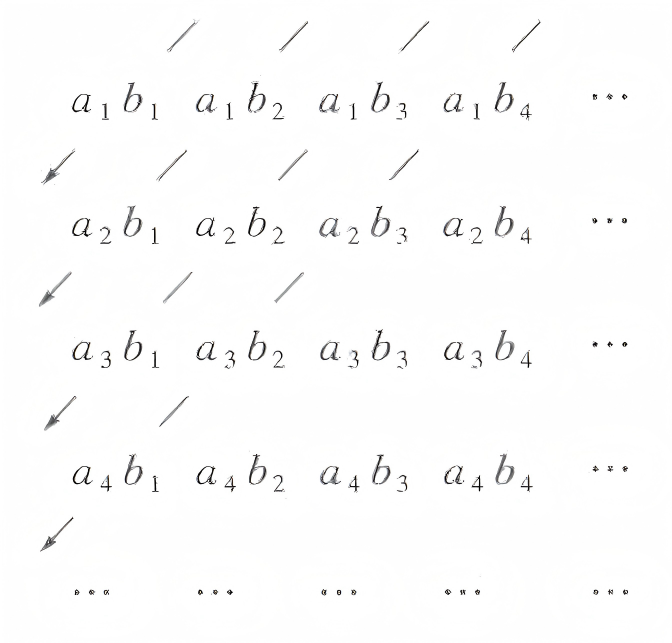
\includegraphics[width=0.4\linewidth]{figure/cauchy(1)}
\end{center}


\[
\begin{aligned}
	c_1 &= a_1 b_1 \\
	c_2 &= a_2 b_1 + a_1 b_2 \\
	&\vdots \\
	c_n &= \sum_{k=1}^n a_k b_{n+1-k}
\end{aligned}
\]
称之为 Cauchy 乘积

2.  正方形排列
\begin{center}
	\centering
	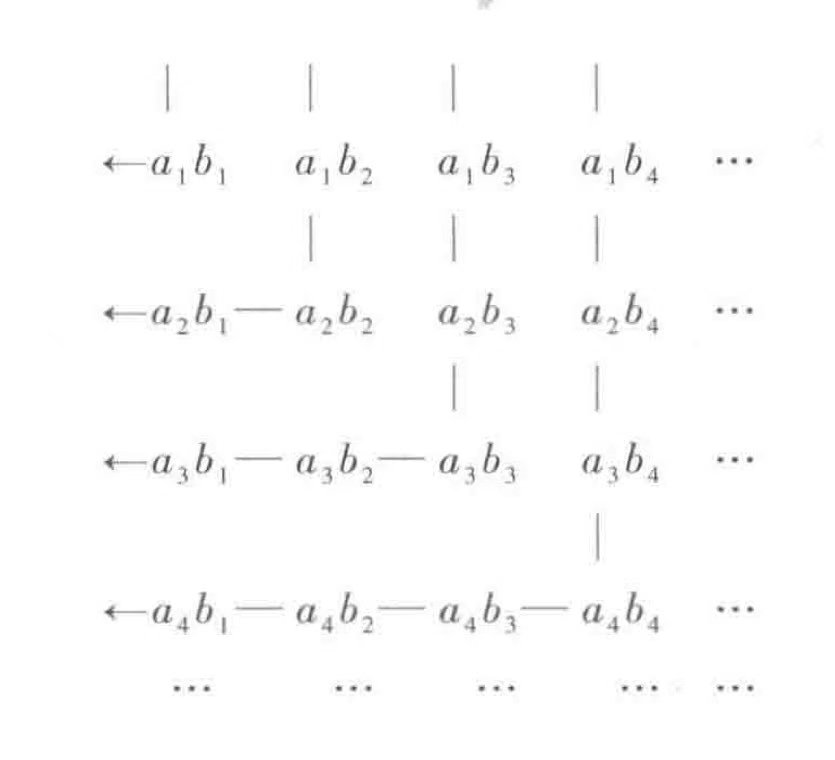
\includegraphics[width=0.4\linewidth]{figure/cubve}
\end{center}


\[
\begin{aligned}
	d_1 &= a_1 b_1 \\
	d_2 &= a_2 b_1 + a_2 b_2 + a_1 b_2 \\
	&\vdots \\
	d_n &= \sum_{k=1}^{n-1} a_n b_k + \sum_{k=1}^{n-1} a_k b_n + a_n b_n
\end{aligned}
\]
其部分和满足：
\[
\sum_{k=1}^n d_k = (a_1 + a_2 + \dots + a_n)(b_1 + b_2 + \dots + b_n)
\]

若级数 $\sum a_n$ 与 $\sum b_n$ 都收敛，则正方形排列的乘积级数 $\sum d_n$ 收敛。设 $\sum a_n = S$，$\sum b_n = T$，则 $\sum d_n = ST$。

但对于 Cauchy 乘积 $\sum c_n$，有可能发散。例如，级数 $\displaystyle \sum_{n=1}^{\infty} \frac{(-1)^{n+1}}{\sqrt{n}}$ 与自身的 Cauchy 乘积发散，而正方形排列的乘积级数收敛。
\begin{proposition}
	（绝对收敛级数的乘积定理）若级数 $\sum a_n$ 与 $\sum b_n$ 都绝对收敛，则将所有乘积项 $a_i b_j$（$i=1,2,\dots; j=1,2,\dots$）按任意方式排列求和而成的级数也绝对收敛，且其和等于
	\[
	\left( \sum_{n=1}^{\infty} a_n \right) \left( \sum_{n=1}^{\infty} b_n \right)
	\]
\end{proposition}
\begin{proof}
	设 $a_{i_k} b_{j_k}$（$k=1,2,\dots$）是所有 $a_i b_j$（$i=1,2,\dots; j=1,2,\dots$）的任意一种排列。对任意正整数 $n$，取
	\[
	N = \max_{1 \le k \le n} \{i_k, j_k\}
	\]
	则
	\[
	\sum_{k=1}^n |a_{i_k} b_{j_k}| \le \sum_{i=1}^N |a_i| \cdot \sum_{i=1}^N |b_i| \le \sum_{n=1}^{\infty} |a_n| \cdot \sum_{n=1}^{\infty} |b_n|
	\]
	因此，级数 $\sum a_{i_k} b_{j_k}$ 绝对收敛。根据绝对收敛级数的重排不变性，其任意更序级数也收敛，且和不变。
	
	设 $\sum d_n$ 是正方形排列下的乘积级数，则 $\sum d_n$ 是 $\sum a_{i_k} b_{j_k}$ 重排后得到的级数。于是
	\[
	\sum_{k=1}^{\infty} a_{i_k} b_{j_k} = \sum_{n=1}^{\infty} d_n = \left( \sum_{n=1}^{\infty} a_n \right) \left( \sum_{n=1}^{\infty} b_n \right)
	\]
\end{proof}
%
% 第5节：无穷乘积
% !TEX root = ../../../main.tex
% 所属：第一部分：单变量分析学 / 第5章：级数理论
% 节：5.5 无穷乘积
% 正文按原文件顺序保存；由 ../chapter5.tex 调用。
\section{无穷乘积}
\begin{definition}
	对数列 $\{p_n\}_{n=1}^{+\infty}$，且对所有 $n \ge 1$，$p_n \neq 0$，称
	\[
	p_1 p_2 \cdots p_n \cdots = \prod_{n=1}^{\infty} p_n
	\]
	为无穷乘积。定义其部分积数列为 $\{P_n\}$：
	\[
	\begin{aligned}
		P_1 &= p_1 \\
		P_2 &= p_1 p_2 \\
		P_3 &= p_1 p_2 p_3 \\
		&\vdots \\
		P_n &= p_1 p_2 \cdots p_n
	\end{aligned}
	\]
	
	若部分积数列 $\{P_n\}$ 收敛于某非零有限数 $P$，则称无穷乘积 $\displaystyle \prod_{n=1}^{\infty} p_n$ 收敛，并称 $P$ 为它的积，记为
	\[
	\prod_{n=1}^{\infty} p_n = P
	\]
	
	若 $\{P_n\}$ 发散，或 $\{P_n\}$ 收敛于 $0$，则称无穷乘积 $\displaystyle \prod_{n=1}^{\infty} p_n$ 发散。
\end{definition}
\begin{proposition}
	若无穷乘积 $\displaystyle \prod_{n=1}^{\infty} p_n$ 收敛，则
	\[
	\lim_{n \to \infty} p_n = 1
	\]
\end{proposition}
\begin{proof}
	设 $\displaystyle \prod_{n=1}^{\infty} p_n = P \neq 0$，那么
	\[
	\lim_{n \to \infty} p_n = \lim_{n \to \infty} \frac{P_n}{P_{n-1}} = \frac{P}{P} = 1
	\]
\end{proof}



从而，我们通常将 $p_n$ 写成 $1 + a_n$ 的形式，即
\[
\prod_{n=1}^{\infty} p_n = \prod_{n=1}^{\infty} (1 + a_n)
\]
由上述命题，若 $\displaystyle \prod_{n=1}^{\infty} p_n$ 收敛，则必有 $a_n \to 0$。

当 $n$ 充分大时，总有 $1 + a_n > 0$，而前有限项不影响无穷乘积的敛散性。因此，下面我们假设：
\begin{itemize}
	\item  对所有 $n$，$1 + a_n > 0$（即 $p_n > 0$）；
	
	\item $a_n \to 0$（即 $p_n \to 1$）。
\end{itemize}
在上述假设下，我们可以建立无穷乘积与无穷级数之间的关系。
\begin{proposition}\label{无穷乘积与无穷级数之间的关系}
	无穷乘积 $\displaystyle \prod_{n=1}^{\infty} p_n = \prod_{n=1}^{\infty} (1 + a_n)$ 收敛，当且仅当级数 $\displaystyle \sum_{n=1}^{\infty} \ln p_n = \sum_{n=1}^{\infty} \ln(1 + a_n)$ 收敛。
	
\end{proposition}
\begin{proof}
	设无穷乘积 $\prod p_n$ 的部分积为 $P_n$，级数 $\sum \ln p_n$ 的部分和为 $S_n$，则有
	\[
	\ln P_n = S_n \quad \Longleftrightarrow \quad P_n = e^{S_n}
	\]
	若 $S_n \to S$ 存在且有限，则 $\lim\limits_{n \to \infty} P_n = e^S$ 存在且有限，故 $\prod p_n$ 收敛。
	反之，若 $P_n \to P$ 存在、有限且大于 $0$，则 $\lim\limits_{n \to \infty} S_n = \ln P$ 存在且有限。
\end{proof}

\begin{corollary}\label{无穷乘积收敛}
	若对所有 $n \ge 1$，$a_n > 0$（或 $a_n < 0$），则无穷乘积 $\displaystyle \prod_{n=1}^{\infty} (1 + a_n)$ 收敛，当且仅当级数 $\displaystyle \sum_{n=1}^{\infty} a_n$ 收敛。
	
\end{corollary}
\begin{proof}
	考虑级数 $\sum \ln(1 + a_n)$ 与 $\sum a_n$。
	若对所有 $n \ge 1$，$a_n > 0$，则 $\ln(1 + a_n) > 0$。
	又因为
	\[
	\lim_{n \to \infty} \frac{\ln(1 + a_n)}{a_n} = 1 \quad (a_n \to 0)
	\]
	由正项级数的比较判别法，$\sum \ln(1 + a_n)$ 与 $\sum a_n$ 有相同的敛散性。
	而由\ref{无穷乘积与无穷级数之间的关系}，$\prod(1 + a_n)$ 与 $\sum \ln(1 + a_n)$ 有相同的敛散性，因此 $\prod(1 + a_n)$ 与 $\sum a_n$ 有相同的敛散性。
	
\end{proof}
\begin{corollary}
	对任意项级数 $\sum a_n$，若 $\sum a_n$ 收敛，则无穷乘积 $\displaystyle \prod_{n=1}^{\infty} (1 + a_n)$ 收敛，当且仅当 $\displaystyle \sum_{n=1}^{\infty} a_n^2$ 收敛。
	
\end{corollary}
\begin{proof}
	由不等式 $\ln(1 + a_n) \le a_n$，可得 $a_n - \ln(1 + a_n) \ge 0$。
	计算极限：
	\[
	\lim_{n \to \infty} \frac{a_n - \ln(1 + a_n)}{a_n^2} = \lim_{x \to 0} \frac{x - \ln(1 + x)}{x^2} = \frac{1}{2}
	\]
	故正项级数 $\sum (a_n - \ln(1 + a_n))$ 与 $\sum a_n^2$ 有相同的敛散性。
	
	若 $\prod(1 + a_n)$ 收敛，则由\ref{无穷乘积与无穷级数之间的关系}，$\sum \ln(1 + a_n)$ 收敛。又已知 $\sum a_n$ 收敛，故 $\sum (a_n - \ln(1 + a_n))$ 收敛，从而 $\sum a_n^2$ 收敛。反之同理可证。
\end{proof}
\begin{definition}
	若级数 $\sum \ln p_n = \sum \ln(1 + a_n)$ 绝对收敛，就称无穷乘积 $\displaystyle \prod_{n=1}^{\infty} p_n = \prod_{n=1}^{\infty} (1 + a_n)$ 绝对收敛。
\end{definition}
\begin{proposition}
	下面三个说法等价：
	\begin{enumerate}
		\item 无穷乘积 $\displaystyle \prod_{n=1}^{\infty} (1 + a_n)$ 绝对收敛；
		\item 无穷乘积 $\displaystyle \prod_{n=1}^{\infty} (1 + |a_n|)$ 收敛；
		\item 级数 $\displaystyle \sum_{n=1}^{\infty} |a_n|$ 收敛。
	\end{enumerate}
\end{proposition}
\begin{proof}
	由\ref{无穷乘积与无穷级数之间的关系}，$\prod(1 + |a_n|)$ 收敛当且仅当 $\sum \ln(1 + |a_n|)$ 收敛。又因为 $|a_n| \ge 0$，由推论 \ref{无穷乘积收敛}，$\sum \ln(1 + |a_n|)$ 收敛当且仅当 $\sum |a_n|$ 收敛，故 2 $\iff$ 3。
	
	下证 1 $\iff$ 3：
	根据定义，$\prod(1 + a_n)$ 绝对收敛 $\iff$ $\sum |\ln(1 + a_n)|$ 收敛。
	考虑极限：
	\[
	\lim_{n \to \infty} \frac{|\ln(1 + a_n)|}{|a_n|} = 1
	\]
	由正项级数的比较判别法，$\sum |\ln(1 + a_n)|$ 与 $\sum |a_n|$ 有相同的敛散性。因此 1 $\iff$ 3。
	
	综上，1、2、3 三个命题等价。
\end{proof}

下面介绍著名的 Wallis 公式与 Stirling 公式，涉及了一定的定积分，读者可以在读完定积分后再读，现在只需记下公式就足够了。
\begin{proposition}（Wallis 公式）
	设 \( p_n = 1 - \dfrac{1}{(2n)^2} \)，则
	\[
	\prod_{n=1}^{\infty} p_n = \frac{2}{\pi}
	\]
\end{proposition}
\begin{proof}
	\[
	\begin{aligned}
		P_n &= \prod_{k=1}^{n} \left(1 - \frac{1}{(2k)^2}\right)
		= \prod_{k=1}^{n} \frac{(2k-1)(2k+1)}{(2k)(2k)} \\
		&= \frac{1 \cdot 3 \cdot 3 \cdot \cdots \cdot (2n-1)(2n+1)}{2 \cdot 2 \cdot 4 \cdot 4 \cdot \cdots \cdot (2n)(2n)}
		= \frac{[(2n-1)!!]^2}{[(2n)!!]^2} \cdot (2n+1)
	\end{aligned}
	\]
	
	考虑定积分 \( I_n = \displaystyle\int_{0}^{\pi/2} \sin^n x \dd x \)。
	后面我们将知道：
	\[
	I_{2n} = \frac{(2n-1)!!}{(2n)!!} \cdot \frac{\pi}{2}, \quad I_{2n+1} = \frac{(2n)!!}{(2n+1)!!}
	\]
	因此
	\[
	\frac{\pi}{2} P_n = \frac{I_{2n}}{I_{2n+1}}
	\]
	
	由不等式 \( I_{2n+1} < I_{2n} < I_{2n-1} \)，得
	\[
	1 < \frac{I_{2n}}{I_{2n+1}} < \frac{I_{2n-1}}{I_{2n+1}}
	\]
	因为
	\[
	\lim_{n \to \infty} \frac{I_{2n-1}}{I_{2n+1}} = \lim_{n \to \infty} \frac{2n+1}{2n} = 1
	\]
	由夹逼性，
	\[
	\lim_{n \to \infty} P_n = \lim_{n \to \infty} \left( \frac{2}{\pi} \cdot \frac{I_{2n}}{I_{2n+1}} \right) = \frac{2}{\pi}
	\]
	故
	\[
	\prod_{n=1}^{\infty} \left(1 - \frac{1}{(2n)^2}\right) = \frac{2}{\pi}
	\]
\end{proof}


换一个形式，就是 Wallis 公式：
\[
\frac{\pi}{2} = \frac{2}{1} \cdot \frac{2}{3} \cdot \frac{4}{3} \cdot \frac{4}{5} \cdot \cdots \cdot \frac{2n}{2n-1} \cdot \frac{2n}{2n+1} \cdot \cdots
\]
\begin{proposition}
	（Stirling 公式）
	\[
	n! \sim \sqrt{2\pi n} \left( \frac{n}{e} \right)^n \quad (n \to +\infty)
	\]
	
\end{proposition}
\begin{proof}
	设 \( b_n = \dfrac{n! e^n}{n^{n+1/2}}, \ n=1,2,\dots \)，则
	\[
	\begin{aligned}
		\frac{b_n}{b_{n-1}} &= e\left(1 - \frac{1}{n}\right)^{n - \frac{1}{2}}
		= \exp\left[1 + \left(n - \frac{1}{2}\right)\ln\left(1 - \frac{1}{n}\right)\right] \\
		&= \exp\left( -\frac{1}{12n^2} + o\left(\frac{1}{n^2}\right) \right)
		= 1 - \frac{1}{12n^2} + o\left(\frac{1}{n^2}\right)
	\end{aligned}
	\]
	
	令 \( 1 + a_n = \dfrac{b_n}{b_{n-1}} \)，于是 \( \sum a_n \) 收敛。那么
	\[
	\prod_{n=2}^{\infty} (1 + a_n) = \prod_{n=2}^{\infty} \frac{b_n}{b_{n-1}}
	\]
	收敛，因此 \( \lim\limits_{n \to \infty} b_n = b_1 \displaystyle\prod_{n=2}^{\infty} \dfrac{b_n}{b_{n-1}} = A \neq 0 \)。
	
	利用 Wallis 公式：
	\[
	A = \lim_{n \to \infty} b_n = \lim_{n \to \infty} \frac{b_n^2}{b_{2n}}
	= \lim_{n \to \infty} \frac{(2n)!!}{(2n-1)!!} \cdot \sqrt{\frac{2}{n}} = \sqrt{2\pi}
	\]
	因此得到 Stirling 公式：
	\[
	n! \sim \sqrt{2\pi n} \left( \frac{n}{e} \right)^n
	\]
\end{proof}
\begin{example}
	证明
	\[
	\sin x=x\prod_{n=1}^{\infty}\left(1-\frac{x^2}{n^2\pi^2}\right).
	\]
\end{example}

\begin{proof}
	由三角函数的知识,我们知道
	\[
	\sin 3\varphi=\sin\varphi\left(3-4\sin^2\varphi\right),
	\]
	\[
	\sin 5\varphi=\sin\varphi\left(5-20\sin^2\varphi+16\sin^4\varphi\right).
	\]
	利用三角恒等式
	\[
	\sin(2k+1)\varphi
	=2(1-2\sin^2\varphi)\sin(2k-1)\varphi-\sin(2k-3)\varphi,
	\]
	以及应用数学归纳法,可以得到
	\[
	\sin(2n+1)\varphi=\sin\varphi\,P(\sin^2\varphi),
	\tag{*}
	\]
	其中 $P(u)$ 是 $n$ 次多项式,它的常数项为
	\[
	P(0)=\lim_{\varphi\to0}\frac{\sin(2n+1)\varphi}{\sin\varphi}=2n+1.
	\]
	由于
	\[
	\varphi=\frac{k\pi}{2n+1}\quad(k=1,2,\cdots,n)
	\]
	使 $(*)$ 式的左端成为 $0$,且
	\[
	\sin^2\frac{k\pi}{2n+1}\quad(k=1,2,\cdots,n)
	\]
	给出 $P(u)$ 的 $n$ 个不同的根,于是
	\[
	P(u)=(2n+1)\prod_{k=1}^{n}
	\left(1-\frac{u}{\sin^2\dfrac{k\pi}{2n+1}}\right).
	\]
	从而得到
	\[
	\sin(2n+1)\varphi
	=(2n+1)\sin\varphi\prod_{k=1}^{n}
	\left(1-\frac{\sin^2\varphi}{\sin^2\dfrac{k\pi}{2n+1}}\right).
	\]
	令 $x=(2n+1)\varphi$,代入后得到
	\[
	\sin x
	=(2n+1)\sin\frac{x}{2n+1}\prod_{k=1}^{n}
	\left(1-\frac{\sin^2\dfrac{x}{2n+1}}{\sin^2\dfrac{k\pi}{2n+1}}\right).
	\]
	因此,当 $m<n$ 时,成立
	\[
	\frac{\sin x}
	{(2n+1)\sin\dfrac{x}{2n+1}
		\displaystyle\prod_{k=1}^{m}
		\left(1-\frac{\sin^2\dfrac{x}{2n+1}}{\sin^2\dfrac{k\pi}{2n+1}}\right)}
	=
	\prod_{k=m+1}^{n}
	\left(1-\frac{\sin^2\dfrac{x}{2n+1}}{\sin^2\dfrac{k\pi}{2n+1}}\right).
	\tag{**}
	\]
	当 $n\to\infty$ 时,$(**)$ 式左端的极限为
	\[
	\frac{\sin x}{x\displaystyle\prod_{k=1}^{m}
		\left(1-\frac{x^2}{k^2\pi^2}\right)}.
	\]
	另一方面,取 $m$ 充分大,使得 $m>|x|/2$.由于
	\[
	\sin^2\frac{x}{2n+1}<\frac{x^2}{(2n+1)^2},
	\]
	并且当 $1\leq k\leq n$ 时,
	\[
	\sin^2\frac{k\pi}{2n+1}
	\geq \frac{4}{\pi^2}\frac{k^2\pi^2}{(2n+1)^2}
	=\frac{4k^2}{(2n+1)^2},
	\]
	故关于 $(**)$ 式的右端,有估计式
	\[
	\begin{aligned}
		1
		&>\prod_{k=m+1}^{n}
		\left(1-\frac{\sin^2\dfrac{x}{2n+1}}{\sin^2\dfrac{k\pi}{2n+1}}\right) \\
		&\geq \prod_{k=m+1}^{n}\left(1-\frac{x^2}{4k^2}\right)
		\geq \prod_{k=m+1}^{\infty}\left(1-\frac{x^2}{4k^2}\right).
	\end{aligned}
	\]
	令 $n\to\infty$,就得到
	\[
	1\geq
	\frac{\sin x}{x\displaystyle\prod_{k=1}^{m}
		\left(1-\frac{x^2}{k^2\pi^2}\right)}
	\geq
	\prod_{k=m+1}^{\infty}\left(1-\frac{x^2}{4k^2}\right).
	\]
	由级数 $\displaystyle\sum_{k=m+1}^{\infty}\frac{x^2}{4k^2}$ 的收敛性,可知无穷乘积
	\[
	\prod_{k=m+1}^{\infty}\left(1-\frac{x^2}{4k^2}\right)
	\]
	收敛,并且当 $m\to\infty$ 时,上述尾乘积趋于 $1$.根据夹逼性,得到
	\[
	\lim_{m\to\infty}
	\frac{\sin x}{x\displaystyle\prod_{k=1}^{m}
		\left(1-\frac{x^2}{k^2\pi^2}\right)}=1.
	\]
	于是
	\[
	\sin x=x\prod_{k=1}^{\infty}\left(1-\frac{x^2}{k^2\pi^2}\right).
	\]
	当 $x=0$ 或 $x=\pm n\pi$ 时,两端显然同为 $0$,故结论对所有 $x$ 成立.
\end{proof}






%

%% ===== 第一部分：单变量分析学 / 第6章：函数的极限与连续性 =====
% !TEX root = ../../main.tex
\setchapterimage{figure/chapter6封面图.png}
\setchapterintro{本章将进入初等分析学中的重点内容——连续性的学习。为了理解连续性，章节首先从函数极限入手，建立函数在一点附近、无穷远处以及左右趋近时的极限概念，再进一步讨论极限的性质，为后面正式研究函数的连续性打基础。
	
	可以概括为一句话：
	
	本章以函数极限为起点，引出并铺垫连续性的学习，这是初等分析学中的核心主题之一。}
\chapter{函数的极限与连续性}
% 第1节：函数极限
% !TEX root = ../../../main.tex
% 所属：第一部分：单变量分析学 / 第6章：函数的极限与连续性
% 节：6.1 函数极限
% 正文按原文件顺序保存；由 ../chapter6.tex 调用。
\section{函数极限}
\begin{definition}\label{def1}
	设函数 $f$ 在点 $x_0$ 的某个去心邻域上有定义，即 $\exists \rho > 0$，使得
	
	$$
	O(x_0, \rho) \setminus \{x_0\} \subset D_f
	$$
	
	对 $A \in \mathbb{R},\text{若} \forall \varepsilon > 0, \exists \delta = \delta(\varepsilon) $ 且 $\delta < \rho$，使得 $\forall x$ 满足 $0 < |x - x_0| < \delta$ 时，
	
	$$
	|f(x) - A| < \eps
	$$
	
	成立，则称 $A$ 为 $f(x)$ 在 $x_0$ 处的极限，记作
	
	$$
	\lim_{x \to x_0} f(x) = A
	$$
	
	若这样的 $A$ 不存在，我们说 $\lim\limits_{x \to x_0} f(x)$ 不存在.
\end{definition}
下面给出 $f(x)$ 在 $x_0$ 的极限不为 $A$ 的定义，这在证明中是经常用的到的.
\begin{definition}\label{nopro}
	$\exists \varepsilon_0 > 0, \forall \delta > 0$，对 $x$，尽管 $0 < |x - x_0| < \delta$，
	
	$$
	|f(x) - A| \geqslant \varepsilon_0
	$$
\end{definition}
接下来我们对极限的定义做出扩展，对$x$的行为以及$f(x)$的行为做出分类，$x$的行为有6种，$f(x)$的行为有4种，两两组合下我们可以得到24种不同极限的定义.

\begin{definition}
	$x$ 的行为：
	
	\begin{enumerate}
		\item $x \to x_0$:~ ————，$\exists \delta > 0, \forall x (0 < |x - x_0| < \delta)$，————
		\item $x \to x_0^+$: ————，$\exists \delta > 0, \forall x (0 < x - x_0 < \delta)$，————
		\item $x \to x_0^-$: ————，$\exists \delta > 0, \forall x (-\delta < x - x_0 < 0)$，————
		\item $x \to \infty$:~~————， $\exists X > 0, \forall x (|x| > X)$，————
		\item $x \to +\infty$: ————，$\exists X > 0, \forall x (x > X)$，————
		\item $x \to -\infty$: ————，$\exists X > 0, \forall x (x < -X)$，————
	\end{enumerate}
	
	其中2、3条与分别对应$x$趋近于$x_0$的左极限与右极限.对函数$f(x)$，$x_0$处 的左右极限记为$f(x_0-),f(x_0+)$
	
	$f(x)$的行为：
	
	\begin{enumerate}
		\item $f(x) \to A$ (有限): $\forall \varepsilon > 0$，————，$  |f(x) - A| < \varepsilon$
		\item $f(x) \to \infty$: $\forall G > 0$，————，$|f(x)| > G$
		\item $f(x) \to +\infty$: $\forall G > 0$，————，$ f(x) > G$
		\item $f(x) \to -\infty$: $\forall G > 0$，————，$ f(x) < -G$
	\end{enumerate}
\end{definition}
举例来说，

$\lim\limits_{x \to x_0} f(x) = \infty$ 定义为

$\forall G > 0, \exists \delta > 0, \forall x$ 满足 $-\delta < x - x_0 < 0$ 有 $|f(x)| > G$ 成立.

$\lim\limits_{x \to +\infty} f(x) = A$ 定义为：

$\forall \varepsilon > 0, \exists X > 0, \forall x$ 满足 $x > X$ 有 $|f(x) - A| < \varepsilon$ 成立.

使用\ref{nopro}中取逆命题的技巧，我们得到一些不收敛于某值，不是无穷的定义

下面给出几个使用定义证明极限的例子.

\begin{example}
	(1)  $$\lim_{x \to 0} e^x = 1$$
	(2)$$\lim_{x \to 1} \frac{x(x-1)}{x^2-1} = \frac{1}{2}$$
	(3)$$\lim_{x \to 1^-} \frac{x^2}{x-1} = -\infty$$
	(4) $$\lim_{x \to \infty} \frac{x+1}{2x-1} = \frac{1}{2}$$
\end{example}
\begin{proof}
	(1) $\forall \varepsilon > 0$，考虑
	\[
	|e^x - 1| < \varepsilon
	\]
	不妨设 $\varepsilon < 1$，
	\[
	1 - \varepsilon < e^x < 1 + \varepsilon
	\]
	取对数得
	\[
	\ln(1 - \varepsilon) < x < \ln(1 + \varepsilon)
	\]
	取 $\delta = \min\{-\ln(1 - \eps), \ln(1 + \eps)\}$，$\forall |x| < \delta$ 都有
	\[
	|e^x - 1| < \varepsilon
	\]
	(2) $\forall \varepsilon > 0$，考虑
	$$\begin{aligned}
		\left|\dfrac{x(x-1)}{x^2-1} - \dfrac{1}{2}\right| &< \varepsilon\\
		\Rightarrow \left|\dfrac{\dfrac{1}{2}(x-1)^2}{x^2-1}\right| &< \eps\\
		\Rightarrow \left|\dfrac{x-1}{2(x+1)}\right| &< \eps
	\end{aligned}$$
	取 $|x-1| < 1$，此时有 $0 < x < 2$，那么 $1 < x+1 < 3$，
	\[
	\left|\dfrac{x-1}{2(x+1)}\right| < \left|\dfrac{x-1}{2}\right| < \eps
	\]
	取 $\delta = \min\{1, 2\varepsilon\}$，$\forall 0 < |x-1| < \delta$ 都有
	\[
	\left|\dfrac{x(x-1)}{x^2-1} - \dfrac{1}{2}\right| < \varepsilon
	\]
	(3) $\forall G > 0$，考虑
	\[
	\frac{x^2}{x-1} < -G
	\]
	取 $-1 < x-1 < 0$，即 $x^2 > 4$，则
	\[
	\frac{x^2}{x-1} < \frac{4}{x-1} < -G
	\]
	取 $\delta = \min\{1, \dfrac{4}{G}\}$，则 $\forall -\delta < x-1 < 0$ 都有
	\[
	\frac{x^2}{x-1} < -G
	\]
	(4) $\forall \varepsilon > 0$，考虑
	$$\begin{aligned}
		\left|\frac{x+1}{2x-1} - \frac{1}{2}\right| &< \varepsilon\\
		\Rightarrow \left|\frac{3}{2(2x-1)}\right| &< \varepsilon
	\end{aligned}$$
	取 $X = \max\left\{\dfrac{3}{4\varepsilon} + \dfrac{1}{2}, \dfrac{3}{-4\varepsilon} - \dfrac{1}{2}\right\}$，$\forall |x| > X$ 都有
	\[
	\left|\frac{x+1}{2x-1} - \frac{1}{2}\right| < \epsilon
	\]
\end{proof}
根据左极限右极限的定义，容易得到以下命题
\begin{proposition}
	$\lim\limits_{x \to x_0} f(x)$ 存在的充要条件是 $f(x)$ 在 $x_0$ 处的左极限、右极限存在并且相等，也就是说：
	\[
	\lim_{x \to x_0} f(x) = A \iff \lim_{x \to x_0^-} f(x) = \lim_{x \to x_0^+} f(x) = A
	\]
\end{proposition}
%
% 第2节：函数极限的性质
% !TEX root = ../../../main.tex
% 所属：第一部分：单变量分析学 / 第6章：函数的极限与连续性
% 节：6.2 函数极限的性质
% 正文按原文件顺序保存；由 ../chapter6.tex 调用。
\section{函数极限的性质}
下面我们叙述函数极限的性质，我们以\ref{def1}中定义的函数极限为例，而其他的23种极限，在有定义的条件下，可以认为下面的性质同样具备.

\begin{proposition}
	设 $A$ 与 $B$ 都是 $f(x)$ 在 $x_0$ 处的极限，即 $A = B$；换句话说，$f(x)$ 在该点的极限唯一.
\end{proposition}
\begin{proof}
	对 $A$ 与 $B$，由极限的定义，
	$$\begin{aligned}
		\forall \varepsilon > 0, &\exists \delta_1 > 0, \forall x (0 < |x - x_0| < \delta_1): |f(x) - A| < \varepsilon\\
		&\exists \delta_2 > 0, \forall x (0 < |x - x_0| < \delta_2): |f(x) - B| < \varepsilon
	\end{aligned}$$
	取 $\delta = \min\{\delta_1,\delta_2\}$，当 $0 < |x - x_0| < \delta$ 时，
	\[
	|A - B| \leqslant |f(x) - A| + |f(x) - B| < 2\varepsilon
	\]
	因为 $\varepsilon$ 是任意的，所以 $|A - B| = 0$，即 $A = B$.
\end{proof}
函数极限有与数列极限相同 的一条性质(\ref{数列的保序性}).

\begin{proposition}
	设 $\lim\limits_{x \to x_0} f(x) = A$，$\lim\limits_{x \to x_0} g(x) = B$，
	
	若 $A > B$，那么存在 $\delta > 0$，使 $0 < |x - x_0| < \delta$ 时，成立 $f(x) > g(x)$.
	\label{partlimits}
\end{proposition}
\begin{proof}
	$$\begin{aligned}
		\forall \varepsilon > 0,&\exists \delta_1 > 0,\forall x (0 < |x - x_0| < \delta_1): |f(x) - A| < \varepsilon\\
		&\exists \delta_2 > 0,\forall x (0 < |x - x_0| < \delta_2): |g(x) - B| < \varepsilon
	\end{aligned}$$
	取 $\delta = \min\{\delta_1, \delta_2\}$，当 $0 < |x - x_0| < \delta$ 时，以上两式同时成立：
	
	再取 $\varepsilon_0 = \dfrac{A - B}{2}$，$\forall \delta, 0 < |x - x_0| < \delta$：
	
	\[
	g(x) < \frac{A + B}{2} < f(x)
	\]
	
\end{proof}
\begin{corollary}
	1. 若 $\lim\limits_{x \to x_0} f(x) = A \neq 0$，则存在 $\delta > 0$，当 $0 < |x - x_0| < \delta$ 时成立
	\[
	|f(x)| > \frac{|A|}{2}
	\]
	
	2. 若 $\lim\limits_{x \to x_0} f(x) = A$，$\lim\limits_{x \to x_0} g(x) = B$，且 $\exists r > 0$，使 $\forall x (0 < |x - x_0| < r)$ 成立 $g(x) \leqslant f(x)$，则 $B \leqslant A$
\end{corollary}
\begin{proof}
	1. 取 \ref{partlimits}中 $f(x) \Rightarrow |f(x)|$，$g(x) \Rightarrow \dfrac{|A|}{2}$，成立.
	
	2. 若不然，则 $B > A$，由 \ref{partlimits}，$\exists \delta > 0$，$\forall x (0 < |x - x_0| < \delta)$ 成立 $f(x) < g(x)$，
	取 $\eta = \min\{\delta, r\}$，当 $0 < |x - x_0| < \eta$ 时，$f(x) < g(x)$ 与 $g(x) \leqslant f(x)$ 矛盾.
	
\end{proof}
\begin{proposition}
	若 $\lim\limits_{x \to x_0} f(x) = A\in\R$，则存在 $\delta > 0$，使得 $f(x)$ 在 $O(x_0, \delta) \setminus \{x_0\}$ 中有界.
\end{proposition}
\begin{proof}
	取 $\varepsilon = 1$，$\exists \delta > 0$，使 $0 < |x - x_0| < \delta$ 时，$|f(x) - A| < \varepsilon = 1$，
	
	即有
	\[
	A - 1 < f(x) < A + 1 \implies |f(x)| < |A| + 1
	\]
	
	即有界.
\end{proof}
\begin{proposition}
	若存在 $r > 0$，使 $\forall x (0 < |x - x_0| < r)$ 成立 $g(x) \leqslant f(x) \leqslant h(x)$，
	
	且 $\lim\limits_{x \to x_0} g(x) = \lim\limits_{x \to x_0} h(x) = A$，则 $\lim\limits_{x \to x_0} f(x) = A$.
\end{proposition}
\begin{proof}
	$$\begin{aligned}
		\forall \varepsilon > 0,&\exists 0 < \delta_1 < r,\forall x (0 < |x - x_0| < \delta_1): A - \varepsilon < g(x)\\
		&\exists 0 < \delta_2 < r,\forall x (0 < |x - x_0| < \delta_2): h(x) < A + \varepsilon
	\end{aligned}$$
	取 $\delta = \min\{\delta_1, \delta_2\}$，当 $0 < |x - x_0| < \delta$，
	\[
	A - \varepsilon < g(x) \leqslant f(x) <h(x) < A + \varepsilon
	\]
	即
	\[
	|f(x) - A| < \varepsilon
	\]
	$\forall x: 0 < |x - x_0| < \delta$
	\[
	\lim_{x \to x_0} f(x) = A
	\]
\end{proof}
\begin{proposition}
	$$\lim_{x\to0}\frac{\sin x}{x}=1$$
\end{proposition}
\begin{proof}
	$x\to0$且$\dfrac{\sin(-x)}{-x}=\dfrac{\sin x}{x}$，不妨设$0<x<\dfrac{\pi}{2}$
	
	考虑下图
	\begin{center}
		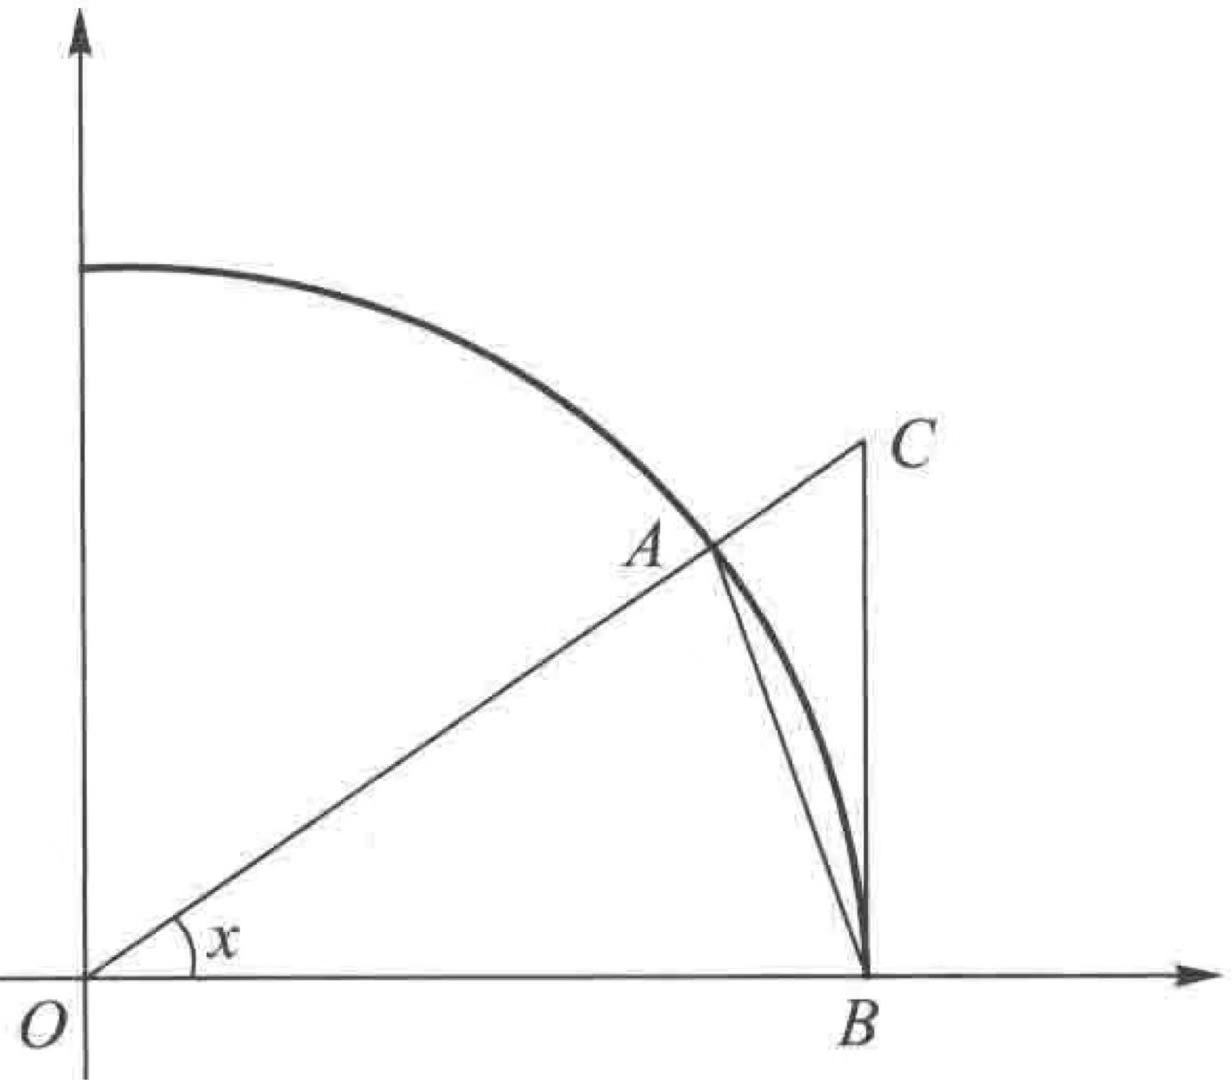
\includegraphics[width=0.3\linewidth]{figure/C5/1}
	\end{center}
	设
	\[
	S_{\triangle OAB} = \frac{1}{2} \sin x = S_1
	\]
	\[
	S_{\triangle OAC} = \frac{1}{2} \tan x = S_2
	\]
	\[
	S_{\textbf{扇形}OAB} = \frac{1}{2} x = S_3
	\]
	
	显然地，
	\[
	S_1 < S_3 < S_2
	\]
	
	也即
	\[
	\sin x < x < \tan x 
	\]
	由于$ x \in \left(0, \dfrac{\pi}{2}\right)$
	\[\frac{\sin x}{x}<1<\frac{\tan x}{x}\Leftrightarrow\cos x<\frac{\sin x}{x}<1\quad x\in(0,\frac{\pi}{2})\]
	下证 $\lim\limits_{x \to 0} \cos x = 1$，也即证明 $f(x) = \cos x$ 在 $x = 0$ 处的连续性.
	
	$\forall \varepsilon > 0$，考虑
	
	\[
	|\cos x - 1| = 2 \sin^2 \frac{x}{2} < \frac{x^2}{2} < \varepsilon
	\]
	
	取 $\delta = \min\left\{\dfrac{\pi}{2}, \sqrt{2\eps}\right\}$，则 $\lim\limits_{x \to 0} \cos x = 1$ 得证.
	
	综上，
	\[
	\lim_{x \to 0} \frac{\sin x}{x} = 1
	\]
\end{proof}
\begin{proposition}
	设 $\lim\limits_{x \to x_0} f(x) = A$，$\lim\limits_{x \to x_0} g(x) = B$，则：
	
	(1) $$\lim_{x \to x_0} (\alpha f(x) + \beta g(x)) = \alpha A + \beta B$$
	
	(2) $$\lim_{x \to x_0} f(x)g(x) = AB$$
	
	(3) $$\lim_{x \to x_0} \frac{f(x)}{g(x)} = \frac{A}{B}\quad B \neq 0$$ 
	
\end{proposition}
\begin{proof}
	$$\begin{aligned}
		\forall \varepsilon > 0,&\exists \delta_1 > 0,\forall x (0 < |x - x_0| < \delta_1): |f(x) - A| < \varepsilon\\
		&\exists \delta_2 > 0,\forall x (0 < |x - x_0| < \delta_2): |g(x) - B| < \varepsilon
	\end{aligned}$$
	
	取 $0 < |x - x_0| < \min\{\delta_1, \delta_2\}$，则两式同时成立.
	
	由有界性：$\forall 0 < |x - x_0| < \min\{\delta_1, \delta_2\}$，$\exists M$，使 $|f(x)| \leqslant M$，$|g(x)| \leqslant M$.
	
	(1)	取 $0 < |x - x_0| < \min\{\delta_1, \delta_2\}$
	\[
	|\alpha f(x) + \beta g(x) - (\alpha A + \beta B)| \leqslant |\alpha||f(x) - A| + |\beta||g(x) - B| < 2\varepsilon
	\]
	
	(2) 取 $0 < |x - x_0| < \min\{\delta_1, \delta_2\}$，
	$$\begin{aligned}
		|f(x)g(x) - AB| &= |f(x)g(x) - g(x)A + g(x)A - AB|\\ 
		&< M|f(x) - A| + |A||g(x) - B| < (M + |A|)\varepsilon
	\end{aligned}$$
	
	
	(3) 取 $0 < |x - x_0| < \min\{\delta_1, \delta_2\}$，
	\[
	\left|\frac{f(x)}{g(x)} - \frac{A}{B}\right| = \left|\frac{Bf(x) - BA + BA - Ag(x)}{Bg(x)}\right| < \frac{2(|A| + |B|)}{B^2} \varepsilon
	\]
	
\end{proof}
\begin{theorem}(Heine定理)\label{Heine1}
	$\lim\limits_{x \to x_0} f(x) = A~\Leftrightarrow~$ $\forall \{x_n\}$ 满足 $x_n \in O(x_0, \rho) \setminus \{x_0\}$ 对某$\rho$，且 $\lim\limits_{n \to \infty} x_n = x_0$，数列 $\{f(x_n)\}$ 满足 $\lim\limits_{n \to \infty} f(x_n) = A$.
\end{theorem}
\begin{proof}
	$\Rightarrow$ 若 $f(x) \to A$ 当 $x \to x_0$，
	
	$\forall \varepsilon > 0, \exists \delta > 0, \forall x (0 < |x - x_0| < \delta): |f(x) - A| < \varepsilon(*)$
	
	由 $x_n \to x_0$，对上述 $\delta > 0, \exists N, \forall n > N$ 
	\[
	0 < |x_n - x_0| < \delta
	\]
	
	由 $(*)$， 因$ x_n \in O(x_0, \rho) \setminus \{x_0\}$，那么 $ |f(x_n) - A| < \varepsilon$
	
	综上$\forall \varepsilon > 0, \exists N, \forall n > N, |f(x_n) - A| < \varepsilon$
	
	$\Leftarrow$ 若不然，$\lim\limits_{x\to x_0}f(x)\neq A$
	
	$\exists \eps_0>0,\forall \delta>0,\exists \widetilde{x},~$即使$0<|\widetilde{x}-x_0|<\delta$，亦有$|f(\widetilde{x})-A|\geqslant\eps_0$
	
	取 $\delta_1 = 1, \exists x_1 (0 < |x_1 - x_0| < \delta_1): |f(x_1) - A| \geqslant \varepsilon_0$，
	
	取 $\delta_2 = \dfrac{1}{2}, \exists x_2 (0 < |x_2 - x_0| < \delta_2): |f(x_2) - A| \geqslant \varepsilon_0$，
	
	$\cdots$
	
	取 $\delta_k = \dfrac{1}{k}, \exists x_k (0 < |x_k - x_0| < \delta_k): |f(x_k) - A| \geqslant \varepsilon_0$，
	
	$\cdots$
	
	这样，我们得到一个列 $\{x_n\}$ 满足 $0 < |x_n - x_0| < \dfrac{1}{n}$ 且 $\lim\limits_{n \to \infty} x_n = x_0$，但是 $|f(x_n) - A| \geqslant \varepsilon_0$，矛盾.
\end{proof}
\begin{corollary}
	(Heine定理的等价叙述)
	$\lim\limits_{x \to x_0} f(x)$ 存在且有限$\Leftrightarrow$对任意序列 $\{x_n\}, x_n \in O(x_0, \rho) \setminus \{x_0\}$ 且 $x_n \to x_0$，$\lim\limits_{n \to \infty} f(x_n)$ 存在且有限.
	
\end{corollary}

\begin{proof}
	必要性$(\Rightarrow)$:同\ref{Heine1}的必要性证明
	
	充分性$(\Leftarrow)$:
	由\ref{Heine1}，只需对任意序列 $\{x_n\}$，$\{f(x_n)\}$ 收敛于同一极限.
	
	如若不然，设 $\{x_n'\}$ 满足 $x_n' \to x_0$，且 $f(x_n') \to A$;$\{x''_n\}$ 满足 $x''_n \to x_0$，且 $f(x''_n) \to B$.
	
	构造数列 $\{x_n\}$ 令 $x_{2n-1} = x_n'$，$x_{2n} = x''_n$，则 $x_n \to x_0$，但 $f(x_n)$ 不收敛，矛盾.
\end{proof}
\begin{example}
	(1) 考虑 $f(x) = \dfrac{a_n x^n + \cdots + a_k x^k}{b_m x^m + \cdots + b_j x^j}$ 在 $x \to 0$ 或 $x \to \infty$ 处的极限.
	
	(2) 证明
	\[
	\lim_{x \to \infty} \left(1 + \frac{1}{x}\right)^x = e
	\]
	
	(3) 证明
	\[
	\lim_{x \to 0} \sin \frac{1}{x} \text{ 不存在}
	\]
\end{example}
\begin{proof}
	(1)
	\[
	\lim_{x \to 0} f(x) =
	\begin{cases}
		\dfrac{a_k}{b_k}, & k = j, \\
		0, & k > j, \\
		\infty, & k < j.
	\end{cases}
	\]
	
	\[
	\lim_{x \to \infty} f(x) =
	\begin{cases}
		\dfrac{a_n}{b_m}, & n = m, \\
		0, & n < m, \\
		\infty, & n > m.
	\end{cases}
	\]
	(2)先考虑$\lim\limits_{x\to+\infty}(1+\dfrac{1}{x})^x$
	
	$\forall x \geqslant 1$，
	\[
	\left(1 + \frac{1}{\lfloor x \rfloor}\right)^{\lfloor x \rfloor} < \left(1 + \frac{1}{x}\right)^x < \left(1 + \frac{1}{\lfloor x \rfloor + 1}\right)^{\lfloor x \rfloor + 1}
	\]
	
	对上式左右两取极限，等价于下式，
	\[
	\lim_{n \to \infty} \left(1 + \frac{1}{n+1}\right)^{n} = e \quad \text{且} \quad \lim_{n \to \infty} \left(1 + \frac{1}{n}\right)^{n+1} = e
	\]
	由夹逼性，
	\[
	\lim_{x \to +\infty} \left(1 + \frac{1}{x}\right)^x = e
	\]
	考虑 $x \to -\infty$ 的情况，令 $y = -x$，$y \to +\infty$，则
	\[
	\lim_{x \to -\infty} \left(1 + \frac{1}{x}\right)^x = \lim_{y \to +\infty} \left(1 - \frac{1}{y}\right)^{-y} = \lim_{y \to +\infty} \left[\left(1 + \frac{1}{y-1}\right)^{y-1} \cdot \left(1 + \frac{1}{y-1}\right)\right] = e
	\]
	综上，
	\[
	\lim_{x \to \infty} \left(1 + \frac{1}{x}\right)^x = e
	\]
	(3) 取 $x_n^{(1)} = \dfrac{1}{n\pi}$，$x_n^{(2)} = \dfrac{1}{2n\pi + \dfrac{\pi}{2}}$，其中 $n = 1, 2, 3, \ldots$
	
	那么 $\lim\limits_{n \to \infty} x_n^{(1)} = \lim\limits_{n \to \infty} x_n^{(2)} = 0$，而 
	$$\lim_{n \to \infty} \sin \frac{1}{x_n^{(1)}} = \lim_{n \to \infty} \sin n\pi = 0,\lim_{n \to \infty} \sin \frac{1}{x_n^{(2)}} = \lim_{n \to \infty} \sin \left(2n\pi + \frac{\pi}{2}\right) = 1$$
	
	由 Heine 定理，$\lim\limits_{x \to 0} \sin \dfrac{1}{x}$ 不存在.
\end{proof}
\begin{proposition}
	(函数极限的Cauchy收敛原理)
	$\lim\limits_{x\to x_0}f(x)$存在且有限
	
	$\Leftrightarrow\forall \varepsilon > 0, \exists \delta > 0, \forall x', x'' \in O(x_0, \delta)\setminus\{x_0\}, |f(x') - f(x'')| < \varepsilon$
	\label{cauchyoffun}
\end{proposition}

\begin{proof}
	$\Rightarrow$:设$\lim\limits_{x \to x_0} f(x) = A$，那么 $\forall \varepsilon > 0, \exists \delta > 0, \forall x', x'' \in O(x_0, \delta) \setminus \{x_0\}$ 都有 $|f(x') - A| < \varepsilon$ 与 $|f(x'') - A| < \varepsilon$.
	
	那么
	\[
	|f(x') - f(x'')| < |f(x') - A| + |f(x'') - A| < 2\varepsilon
	\]
	
	$\Leftarrow$:已知$\forall \varepsilon > 0, \exists \delta > 0, \forall x',x'' \in O(x_0, \delta) \setminus\{x_0\}$ 有 $|f(x') - f(x'')| < \varepsilon$.
	
	$\forall \{x_n\}$使得$\{f(x_n)\}$有定义，且收敛于 $x_0$，对上述的 $\delta$，有
	$$\begin{aligned}
		\exists N, &\forall n > N,\textbf{有} |x_n - x_0| < \delta\\
		&\forall p > 0,\textbf{有} |x_{n+p} - x_0| < \delta
	\end{aligned}$$
	那么
	\[
	|f(x_n) - f(x_{n+p})| < \varepsilon
	\]
	
	因此 $\{f(x_n)\}$ 是 Cauchy 列，所以 $\{f(x_n)\}$ 收敛，由 Heine 定理，$\lim\limits_{x \to x_0} f(x)$ 存在且有极限
	
\end{proof}
注意：对24种不同的极限，在有定义 的情况下都有相应的Cauchy收敛原理，相应的证法各有不同，下举一例

\begin{example}
	$\lim\limits_{x \to +\infty} f(x)$ 存在且有限
	
	$\Leftrightarrow \forall \varepsilon > 0, \exists X, \text{使得} \, \forall x', x'' > X, \text{都有} \, |f(x') - f(x'')| < \varepsilon$
\end{example}
\begin{proof}
	$\Rightarrow$ 同 \ref{cauchyoffun} ，略
	
	$\Leftarrow$ 已知 $\forall \varepsilon > 0, \exists X > 0, \text{使得} \, \forall x', x'' > X  \text{都有} \, |f(x') - f(x'')| < \varepsilon$.
	
	$\forall \{x_n\}$ 满足 $x_n \to +\infty$，则 $\exists N, \forall n > N, \text{有} \, x_n > X$.
	
	对上述 $X$，$\exists N, \forall n > N, \text{有} \, x_n > X$，$\forall p > 0, \text{有} \, x_{n+p} > X$，则
	\[
	|f(x_n) - f(x_{n+p})| < \varepsilon
	\]
	
	因此，$\{f(x_n)\}$ 是一个 Cauchy 列，则 $\{f(x_n)\}$ 收敛且有界.由 Heine 定理，$\lim\limits_{x \to +\infty} f(x)$ 存在且有限.
\end{proof}

%
% 第3节：连续性
% !TEX root = ../../../main.tex
% 所属：第一部分：单变量分析学 / 第6章：函数的极限与连续性
% 节：6.3 连续性
% 正文按原文件顺序保存；由 ../chapter6.tex 调用。
\section{连续性}
\begin{definition}
	对 函数$f(x)$，若满足：
	\begin{enumerate}
		\item $f(x) $在$ O(x_0, \rho)$ 上有定义，对某 $\rho$(此处无需去心邻域)
		\item $\lim\limits_{x \to x_0} f(x)$ 存在
		\item $\lim\limits_{x \to x_0} f(x) = f(x_0)$
	\end{enumerate}
	
	就说 $f(x)$ 在 $x_0$ 处连续.或等价地，用“$\varepsilon-\delta$”语言：
	
	$f(x) $在$ O(x_0, \rho)$ 上有定义，对某 $\rho$，$\forall \varepsilon > 0$，$\exists \delta(\varepsilon, x_0)> 0$，$\forall x (|x - x_0| < \delta)$：
	\[
	|f(x) - f(x_0)| < \varepsilon
	\]
	
\end{definition}
\begin{definition}
	对 $f(x)$，若：
	\begin{itemize}
		\item $f(x)$ 在 $[x_0, x_0 + \rho)$ 上有定义，且 $\lim\limits_{x \to x_0^+} f(x) = f(x_0)$，则称 $f(x)$ 在$x_0$右连续.
		\item $f(x)$ 在 $(x_0 - \rho, x_0]$ 上有定义，且 $\lim\limits_{x \to x_0^-} f(x) = f(x_0)$，则称 $f(x)$ 在$x_0$左连续.
	\end{itemize}
	显然，若 $f(x)$ 在 $x_0$ 处连续，则必有
	\[
	\lim_{x \to x_0^+} f(x) = \lim_{x \to x_0^-} f(x) = f(x_0)
	\]
\end{definition}

\begin{definition}
	若 $f(x)$ 在开区间 $(a, b)$ 上的任意一点处连续，那么称 $f(x)$ 在开区间 $(a, b)$ 上连续.记为$f\in C(a,b)$.
	
	若 $f(x)$ 在 $(a, b)$ 上连续，同时在 $x = a$ 处右连续，在 $x = b$ 处左连续，那么称 $f(x)$ 在闭区间 $[a, b]$ 上连续.记为$f\in C[a,b]$
	
	
\end{definition}
\begin{proposition}
	
	设 $f(x), g(x)$ 在 $x_0$ 处连续，那么有
	
	(1) $$\lim_{x \to x_0} (\alpha f(x) + \beta g(x)) = \alpha f(x_0) + \beta g(x_0)$$
	
	更一般地，有限个连续函数的线性组合仍连续，而无限个连续函数的“线性组合”未必连续，甚至未必有意义.
	
	(2) $$\lim_{x \to x_0} f(x)g(x) = f(x_0)g(x_0)$$
	
	更一般地，有限个连续函数的乘积仍连续，无限个连续的乘积则未必，甚至未必有定义
	
	(3) $$\lim_{x \to x_0} \frac{f(x)}{g(x)} = \frac{f(x_0)}{g(x_0)}\quad g(x_0) \neq 0$$ 
\end{proposition}
\begin{proof}
	由函数极限的定义的易知
\end{proof}

考虑 $f(x)$ 在 $x_0$ 处连续的定义：
\begin{enumerate}
	\item 在 $x_0$ 处左右极限存在且相等；
	\item 在 1 下，$\lim\limits_{x \to x_0^+} f(x) =\lim\limits_{x \to x_0^-} f(x)= f(x_0)$
\end{enumerate}

逐一的破坏极限的定义，我们得出 $f(x)$在$x_0$ 的三类不连续点的定义.
\begin{definition}
	设 $f(x)$ 在 $x_0$ 的某邻域内有定义
	\begin{enumerate}
		\item  若 $f(x)$ 在 $x_0$ 处的左右极限存在，且 $f(x_0-) \neq f(x_0+)$，则称 $x_0$ 为第一类间断点，又称跳跃间断点（$|f(x_0+) - f(x_0-)|$ 为 $x_0$ 上的跃度）.
		\item 若 $f(x)$ 在 $x_0$ 处的左右极限至少有一不存在，则称 $x_0$ 为第二类间断点.
		\item 若 $f(x)$ 在 $x_0$ 处的左右极限都存在且相等，但 $f(x_0+) = f(x_0-) \neq f(x_0)$，则称 $x_0$ 为第三类间断点.此时，令	
		\[
		\widetilde{f}(x) = \begin{cases}
			f(x) & x \neq x_0 \\
			f(x_0+) = f(x_0-) & x = x_0
		\end{cases}
		\]
	\end{enumerate}
	在 $f$ 无其他不连续点的情况下，$\widetilde{f}(x)$ 是连续的.第三类间断点又称可去间断点.
	
	有些时候，$f$ 在 $x_0$ 处无定义，我们把这种情况也归入第三类间断点
	
	还有一种间断点，顾名思义的，无穷间断点，因各个教材的分类不同，此处单取一类
\end{definition}
我们给出几个例子

\begin{example}
	考虑从下列函数的不连续点以及不连续点的类型：
	
	(1) $f(x) = \dfrac{\sin x}{x}$
	
	(2) $D(x) = \begin{cases}
		1, & x \in \mathbb{Q} \\
		0, & x \in \mathbb{R} \setminus\mathbb{Q}
	\end{cases}$
	
	(3) $R(x) = \begin{cases}
		\dfrac{1}{p}, & x = \dfrac{q}{p}, p\in\Z_+,q\in\Z\setminus\{0\},\text{$p$ 和 $q$ 互质}\\
		1, & x = 0 \\
		0, & x \in \mathbb{R} \setminus \mathbb{Q}
	\end{cases}$
	
	(4) $g(x) = \text{sgn}(x)$
\end{example}
\begin{proof}
	1. 函数 \( f(x) \) 在 \( x = 0 \) 处无定义，但 \(\lim\limits_{x \to 0^+} \dfrac{\sin x}{x} = \lim\limits_{x \to 0^-} \dfrac{\sin x}{x} = 1\)，故 \( x = 0 \) 是第三类间断点；
	
	2. 对 \(\forall x_0 \in \mathbb{R}\)，考虑两个列 $\{x_n\},\{y_n\}$满足 \(x_n \in \mathbb{Q}, y_n \in \mathbb{R} \setminus \mathbb{Q}\)，
	且 \(x_n, y_n < x_0\)，\(x_n, y_n \to x_0\)，那么
	\[
	\lim_{n \to \infty} D(x_n) = 1, \quad \lim_{n \to \infty} D(y_n) = 0
	\]
	
	由 Heine 定理 \(\lim\limits_{x \to x_0} D(x)\) 不存在，即 \(D(x)\) 在 \(x_0\) 处间断.故任意一点都是第二类间断点.
	
	(3) $R(x+1) = R(x)$，故 $R(x)$ 是 1 为周期的函数，只需考虑 $[0,1]$ 这一区间上的点即可.
	
	对任意无理点 $x_0 \in \mathbb{R} \setminus \mathbb{Q}$，对 $R(x_0) = 0$ 且 $\lim\limits_{x \to x_0} R(x) = 0$，故在任意无理点处连续.
	
	下面考虑 $[0,1]$ 上的有理数 $x_0$，下证 $\lim\limits_{x \to x_0} R(x) = 0$.
	
	$\forall \varepsilon > 0$，考虑 $|R(x)| < \varepsilon$，求相应的$\delta$.
	
	反向的考虑：在 $[0,1]$ 的区间里，$R(x) \geqslant \varepsilon$ 的点有多少个.
	
	$\eps>0,\exists n$，使得$\dfrac{1}{10^{n-1}}>\eps\geqslant \dfrac{1}{10^n}$，$R(x)>\dfrac{1}{10^n}$
	
	比如 ,$n=1$ 时，$R(x) = 1, \dfrac{1}{2}, \dots, \dfrac{1}{9}>\dfrac{1}{10}$;$n=2$ 时，$R(x) = 1, \dfrac{1}{2}, \dots, \dfrac{1}{99}>\dfrac{1}{100}$
	
	显然，使 $R(x) > \dfrac{1}{10^n}$ 的有理数 $x \in [0,1]$ 是有限的.设为 $x_1, \dots, x_n$，假设其中不含$x_0$,$\forall1\leqslant k\leqslant n,|x_k - x_0|>0$，取 $\delta= \min\limits_{1 \leqslant k \leqslant n} |x_k - x_0|>0$.则 $0 < |x - x_0| < \delta$ 时，$R(x) < \varepsilon$.
	
	综上 $\lim\limits_{x \to x_0} R(x) = 0$而$R(x_0) = \dfrac{1}{p}$，故在有理点上不连续，属第二类间断点.
	
	(4) 显然，$\lim\limits_{x \to 0^-} \text{sgn}(x) = -1$，$\lim\limits_{x \to 0^+} \text{sgn}(x) = 1$，而 $\text{sgn}(0) = 0$.故 $x = 0$ 为第一类间断点，且跃度为 2.
\end{proof}
\begin{proposition}
	设函数 $f$ 在区间 $(a, b)$ 上单调，那么$(a, b)$ 中使$f$ 间断的点的集是至多可数.
\end{proposition}

\begin{proof}
	设 $E$ 是 $f$ 所有间断点构成的集合，假设$f$是单调递增的.对于 $\forall x \in E$，$\exists r \in \mathbb{Q},r=r(x)$，使得 $f(x-) < r(x) < f(x+)$.
	
	由 $x_1 < x_2$，若 $f(x_1+) \leqslant f(x_2-)$，所以$x_1 \neq x_2$ 时，$r(x_1) \neq r(x_2)$.
	
	因此，在 $E$ 与 $\mathbb{Q}$ 的子集上建立了一一对应.
\end{proof}
\begin{proposition}
	$(a, b)$ 上的单调函数(未必严格单调)的不连续点必为第一类间断点.
	\label{monouni}
	
\end{proposition}
\begin{proof}
	不妨设函数 $f(x)$ 单调上升，
	
	令 $S = \{ f(x): x \in (a, x_0) \}$.
	
	因 $f\left(\dfrac{x_0 + a}{2}\right) \in S$ 故 $S \neq \varnothing$ 且有上界（$f(x_0)$ 是 $S$ 的一个上界）.
	
	那么，由确界原理 $\beta = \sup S$ 存在.
	
	对 $\beta = \sup S$，$\forall \varepsilon > 0$，$\exists x^* \in (a, x_0)$，使 $f(x^*) > \beta - \varepsilon$.
	
	取 $\delta = x_0 - x^* > 0$，当 $x \in (x_0 - \delta, x_0)$，$x^* < x < x_0$，
	
	$$\beta - \varepsilon < f(x^*) \leqslant f(x) \leqslant \beta \Leftrightarrow-\eps<f(x)-\beta\leqslant0$$
	
	因此 $f(x_0-)$ 存在，同理 $f(x_0+)$存在.
\end{proof}
下面我们考虑连续性之于反函数
\begin{proposition}\label{infunex}
	证明：$f(x)$ 在 $D_f \subset \mathbb{R}$ 上严格单调增（或严格单调减），则 $y = f(x)$ 的反函数 $x = f^{-1}(y)$：$R_f \to D_f$ 存在，且 $f^{-1}(y)$ 也为严格单调增（或严格单调减）.
	
\end{proposition}
\begin{proof}
	
	存在性：由 $f$ 是严格单调，$f^{-1}$ 满足映射定义一 对一的条件，存在性得证.
	
	单调性：设 $f$ 是严格单调增，
	若 $f^{-1}$ 不严格单调增，则$f^{-1}$为单调减，那么 $\forall y_1, y_2 \in R_f$，设 $y_1 < y_2$，但 $x_1 = f^{-1}(y_1) \geqslant x_2 = f^{-1}(y_2)$，又因 $f$ 单增，$x_1 \geqslant x_2$，$f(x_1) \geqslant f(x_2)$ 矛盾.
	
\end{proof}
\begin{proposition}
	设函数 $y = f(x)$ 在闭区间 $[a, b]$ 上连续且严格单调增，$f(a) = \alpha$，$f(b) = \beta$，则其反函数 $x = f^{-1}(y)$ 在 $[\alpha, \beta]$ 上连续且严格单调增.
	
	
\end{proposition}
\begin{proof}
	先证$\forall y_0 \in [\alpha, \beta]$，$\exists x_0 \in [a, b]$，使得 $f(x_0) = y_0$，换言之$$f([a, b]) = [\alpha, \beta]$$
	
	设 $\gamma \in (\alpha, \beta)$，设
	$$S = \{x : x \in [a, b], f(x) < \gamma
	\}$$
	由$a\in S$,$S$ 非空，且 $f(b) > \gamma$，$S$ 有上界，由确界原理，$\exists x_0 = \sup S$，$x_0 \in (a, b)$.
	由 $f$ 单调递增，$x<x_0$时，$f(x)<\gamma$;$x>x_0$时，$f(x)>\gamma$.由\ref{monouni}
	$$f(x_0-) \leqslant \gamma \leqslant f(x_0+)$$
	而 $f$ 在 $x_0$ 处连续，$f(x_0) =f(x_0+)=f(x_0-)= \gamma$，这样$f$ 的值域是 $[\alpha, \beta]$
	
	由\ref{infunex}，在 $[\alpha, \beta]$ 上存在$f$的反函数$x=f^{-1}(y)$，且 $f^{-1}$ 严格单调增.
	
	下证 $f^{-1}$ 在 $[\alpha, \beta]$ 上的连续性：
	
	设 $y_0 \in (\alpha, \beta)$，相应的有 $f^{-1}(y_0) = x_0 \in (a, b)$.对于任意 $\varepsilon > 0$，找出$\delta > 0$，使得 $|y - y_0| < \delta$ 时，
	有 
	$$|f^{-1}(y)-f^{-1}(y_0)|=|f^{-1}(y)-x_0|<\eps$$
	即$$x_0-\eps<f^{-1}(y)<x_0+\eps$$
	设$y_1 = f(x_0 - \varepsilon),y_2 = f(x_0 + \varepsilon)$
	，令 $\delta = \min\{|y_1 - y_0|, |y_2 - y_0|\}$
	
	$\forall y$ 满足 $|y - y_0| < \delta$，$f^{-1}(y) \in (x_0 - \varepsilon, x_0 + \varepsilon)$，即 $f^{-1}$ 连续.
	
\end{proof}
\begin{proposition}
	设 $u = g(x)$ 在 $x = x_0$ 处连续，$u_0 = g(x_0)$；$y = f(u)$ 在 $u = u_0$ 处连续，则 $y = f \circ g(x)$ 在 $x = x_0$ 处连续，且 $y_0 = f \circ g(x_0)$.
	
	
\end{proposition}
\begin{proof}
	设函数的值域在所讨论的区间中有定义
	
	由 $y = f(u)$ 在 $u = u_0$ 处连续，$\forall \varepsilon > 0$，$\exists \eta > 0$，使 $|u - u_0| < \eta$ 时，
	\[ |f(u) - f(u_0)| < \varepsilon \]
	
	$u = g(x)$ 在 $x = x_0$ 处连续，对上述 $\eta > 0$，$\exists \delta > 0$，使 $|x - x_0| < \delta$ 时，
	\[ |g(x) - g(x_0)| < \eta \Leftrightarrow|u - u_0| < \eta \]
	
	因此，对 $\delta$，$|x-x_0|<\delta$时，
	\[ |f \circ g(x) - f \circ g(x_0)| < \varepsilon \]
	
	即 $f \circ g$ 在 $x = x_0$ 处连续.
\end{proof}
\begin{corollary}
	有限多连续函数的复合依旧是连续的
\end{corollary}
\begin{proof}
	用数学归纳法即可证明
\end{proof}
%
% 第4节：基本初等函数的连续性
% !TEX root = ../../../main.tex
% 所属：第一部分：单变量分析学 / 第6章：函数的极限与连续性
% 节：6.4 基本初等函数的连续性
% 正文按原文件顺序保存；由 ../chapter6.tex 调用。
\section{基本初等函数的连续性}
下面我们考虑各个基本初等函数的连续性.
\begin{proposition}
	显然的，常数函数$f(x)=c(\text{常数})$在定义域上是连续的
\end{proposition}
\begin{proposition}
	$f(x)=x^{\alpha}\quad \alpha\in\R$在定义域上是连续的
\end{proposition}
\begin{proof}
	对 $\alpha \in \mathbb{Z}$，先考虑 $f(x) = x\quad x\in(-\infty, +\infty)$，
	
	$\forall \varepsilon > 0$，取 $\delta = \varepsilon$，$\forall x(0 < |x - x_0| < \delta)$，
	\[ |f(x) - f(x_0)| = |x - x_0| < \varepsilon = \delta \]
	
	$\alpha \in \mathbb{Z}$ 时，$x^\alpha$ 可以看作 $\alpha$ 个 $x$ 的乘积，自然为连续函数
	
	对 $\alpha \in \mathbb{Q}$，先考虑 $f(x) = \sqrt[m]{x}$
	
	$m \in \mathbb{Z}_+$，
	$\forall \varepsilon > 0$，取 $\delta = \varepsilon^m$，$\forall x(0 < |x - x_0| < \delta)$，
	\[ |\sqrt[m]{x} - \sqrt[m]{x_0}| \leqslant\sqrt[m]{|x-x_0|}<\varepsilon \]
	
	$\alpha \in \mathbb{Q}$ ，设 $\alpha = \dfrac{n}{m}$，$f(x) = x^{n/m}$，由复合函数的连续性，对 $\alpha \in \mathbb{Q}$，$x^{\alpha}$在定义域上连续
	
	对 $\alpha \in \mathbb{R} \setminus\mathbb{Q}$，我们之后再说
	
\end{proof}
\begin{proposition}
	函数 $f(x) = a^x$ ($a > 0$, $a \neq 1$) 在 $(-\infty, +\infty)$ 上连续.
\end{proposition}
\begin{proof}
	$\forall x_0 \in (-\infty, +\infty)$，
	\[ a^x - a^{x_0} = a^{x_0}(a^{x - x_0} - 1) \]
	
	因为
	\[ \lim_{x \to x_0} a^x = a^{x_0} \Leftrightarrow \lim_{t \to 0} a^t = 1 \]
	$t \to 0^+$ 时，当 $a > 1$时，有
	\[ 1 < a^t \leqslant a^{1/[\frac{1}{t}]} \]
	而 $\lim\limits_{n \to \infty} a^{1/n} = 1$，由夹逼定理，
	\[ \lim_{t \to 0^+} a^t = 1 \]
	
	$0 < a < 1$ 时，
	\[ \lim_{t \to 0^+} a^t = \lim_{t \to 0^+} \dfrac{1}{\left(\dfrac{1}{a}\right)^t} = 1 \]
	
	$t \to 0^-$ 时，令 $u = -t$，
	\[ \lim_{t \to 0^-} a^t = \lim_{u \to 0^+} a^{-u} = \lim_{u \to 0^+} \frac{1}{a^u} = 1 \]
	
	综上，
	\[ \lim_{t \to 0} a^t = 1 \]
	从而 $\lim\limits_{x \to x_0} a^x = a^{x_0}$.
	
\end{proof}
\begin{corollary}
	$f(x)=\log_a(x)$在定义域上是连续的
\end{corollary}
\begin{proof}
	由$f(x)=a^x$以及反函数连续性定理易得
\end{proof}
\begin{corollary}
	$f(x)=x^{\alpha},\alpha\in\R$在定义域上连续
	
\end{corollary}
\begin{proof}
	$$f(x)=x^{\alpha	}=e^{\alpha\ln x}$$
	由复合函数连续性定理得证
	
\end{proof}
\begin{corollary}
	双曲函数$$\begin{aligned}
		&y=\sinh x &y=\cosh x \quad &y=\tanh x\\
		&y=\mathrm{csch}x &y=\mathrm{sech}x\quad&y=\coth x
	\end{aligned}$$在定义域上是连续的
\end{corollary}
\begin{proposition}
	函数 $f(x) = \sin x$ 与 $g(x) = \cos x$ 在 $(-\infty, +\infty)$ 上连续.
\end{proposition}
\begin{proof}
	对于 $y = \sin x$，$\forall x_0 \in (-\infty, +\infty)$，
	\[
	|\sin x - \sin x_0| = 2 \left|\cos \frac{x_0 + x}{2} \sin \frac{x - x_0}{2}\right| \leqslant |x - x_0|
	\]
	取 $\delta = \varepsilon$，当 $|x - x_0| < \delta$ 时，
	\[
	|\sin x - \sin x_0| < \varepsilon
	\]
	
	对于 $y = \cos x$，$\forall x_0 \in (-\infty, +\infty)$，
	\[
	|\cos x - \cos x_0| = 2 \left|\sin \frac{x_0 + x}{2} \sin \frac{x - x_0}{2}\right| \leqslant |x - x_0|
	\]
	取 $\delta = \varepsilon$，当 $|x - x_0| < \delta$ 时，
	\[
	|\cos x - \cos x_0| < \varepsilon
	\]
	
\end{proof}
\begin{corollary}
	$y=\tan x,y=\cot x,y=\csc x,y=\sec x$在定义域上 是连续的
\end{corollary}

\begin{corollary}
	反三角函数
	\[ y = \sin^{-1} x, \quad y = \cos^{-1} x, \quad y = \tan^{-1} x \]
	\[ y = \csc^{-1} x, \quad y = \sec^{-1} x, \quad y = \cot^{-1} x \]
	在其定义域内连续
\end{corollary}
\begin{corollary}
	基本初等函数的有限次复合函数在其定义域上连续	
\end{corollary}
%
% 第5节：无穷大量与无穷小量的阶
% !TEX root = ../../../main.tex
% 所属：第一部分：单变量分析学 / 第6章：函数的极限与连续性
% 节：6.5 无穷大量与无穷小量的阶
% 正文按原文件顺序保存；由 ../chapter6.tex 调用。
\section{无穷大量与无穷小量的阶}
下面我们介绍阶数这一概念，类似于集合的势的比较，我们定义的阶数揭示了无穷小量趋近于零的相对程度以及无穷大量绝对增长至无穷的相对程度

类似于数列极限中对无穷大量与无穷小量的定义，下面是函数极限中无穷大量与无穷小量 的定义
\begin{definition}
	若 $\lim\limits_{x \to A} f(x) = 0$，则称 $x \to A$ 时 $f(x)$ 是无穷小量.
	
	若 $\lim\limits_{x \to A} f(x) = \infty(\pm\infty
	)$ ，则称 $x \to A$ 时 $f(x)$ 是无穷大量.
	
	这里 $x \to A$ 包括了 $x \to x_0$，$x \to x_0^+$，$x \to x_0^-$，$x \to +\infty$，$x \to -\infty$，$x \to \infty$ 等各种情况，下面用 $x \to x_0$ 举例.
	
\end{definition}
无穷大量与无穷小量的阶定义如下，它是一种相对的定义我们可以说两个无穷量的阶数如何如何，想要给出某一无穷量的绝对阶数，需要与$x^a$做比对
\begin{definition}
	对于 $u(x), v(x)$，当 $x \to x_0$ 时，$u(x), v(x)$ 都是无穷小量.
	
	(1) 若 $\lim\limits_{x \to x_0} \dfrac{u(x)}{v(x)} = 0$，我们称 $x \to x_0$ 时，$u(x)$ 关于 $v(x)$ 是高阶无穷小量或 $v(x)$ 关于 $u(x)$ 是低阶无穷小量，记作
	\[ u(x) = o(v(x)) \quad (x \to x_0). \]
	
	(2) 若 $\exists A > 0$，当$x$ 在$x_0$的某邻域内，成立
	\[ \left| \frac{u(x)}{v(x)} \right| \leqslant A \]
	则称 $x \to x_0$ 时，$\dfrac{u(x)}{v(x)}$ 是有界量，记作
	\[ u(x) = O(v(x)) \quad (x \to x_0). \]
	
	(3) 若 $\exists A\geqslant a > 0$，对于 $x$ 在$x_0$的某去心邻域内，成立
	\[ a \leqslant \left| \frac{u(x)}{v(x)} \right| \leqslant A \]
	则称 $x \to x_0$ 时，$u(x)$ 与 $v(x)$ 是同阶无穷小量.
	
	若 $\lim\limits_{x \to x_0} \dfrac{u(x)}{v(x)} = C \neq 0$，则 $u(x)$ 与 $v(x)$ 必是同阶无穷小量.
	
	(4) 若 $\lim\limits_{x \to x_0} \dfrac{u(x)}{v(x)} = 1$，则称 $x \to x_0$ 时，$u(x)$ 与 $v(x)$ 是等价无穷小量，记作
	\[ u(x) \sim v(x) \quad (x \to x_0). \]
	
	也可以写成
	\[ u(x) = v(x) + o(v(x)) \quad (x \to x_0). \]
	
	表示$x \to x_0$ 时，$u(x)$ 与 $v(x)$ 不一定相等，差一个关于 $v(x)$ 的高阶无穷小量，
	
\end{definition}
\begin{example}
	(1)
	\[
	\lim_{x \to 0} \frac{1 - \cos x}{x} = \lim_{x \to 0} \dfrac{2 \sin^2 \dfrac{x}{2}}{x} = 0
	\]
	所以
	\[
	1 - \cos x = o(x) \quad (x \to 0)
	\]
	
	(2)
	\[
	\lim_{x \to 0} \frac{\tan x - \sin x}{x^2} = \lim_{x \to 0} \left( \frac{\sin x}{x \cos x} \cdot \frac{1 - \cos x}{x} \right) = 0
	\]
	所以
	\[
	\tan x - \sin x = o(x^2) \quad (x \to 0)
	\]
	
	(3)$x \to 0 $时，$x \sin \dfrac{1}{x}$ 是无穷小量，且$\left| \dfrac{x \sin \dfrac{1}{x}}{x} \right| \leqslant 1$，因此 
	\[
	x \sin \frac{1}{x} = O(x) \quad (x \to 0)
	\]
	
	(4)
	\[
	\lim_{x \to 0} \frac{\sin x}{x} = 1
	\]
	所以
	\[
	\sin x \sim x \quad (x \to 0) \quad \text{ 或者 } \quad \sin x = x + o(x) \quad (x \to 0)
	\]
	
	(5)
	\[
	\lim_{x \to 0} \dfrac{1 - \cos x}{\dfrac{1}{2} x^2} = \lim_{x \to 0} \dfrac{2 \sin^2 \dfrac{x}{2}}{\dfrac{1}{2} x^2} = 1
	\]
	所以
	\[
	1 - \cos x \sim \frac{1}{2} x^2 \quad (x \to 0) \quad \text{ 或者 } \quad 1 - \cos x = \frac{1}{2} x^2 + o(x^2) \quad (x \to 0)
	\]
	
	(6)
	\[
	\lim_{x \to 0} \frac{\tan x - \sin x}{\dfrac{1}{2} x^3} = \lim_{x \to 0} \left( \frac{\sin x}{x \cos x} \cdot \dfrac{1 - \cos x}{\dfrac{1}{2} x^2} \right) = 1
	\]
	所以
	\[
	\tan x - \sin x \sim \dfrac{1}{2} x^3 \quad (x \to 0)\text{或者}\tan x - \sin x=\frac{1}{2}x^3+o(x^3)\quad(x\to0)\]
\end{example}
我们往往取 $v(x) = (x - x_0)^k$ 与 $u(x)$ 进行比较 ($x \to x_0$)，若 $x \to \infty$，
则取 $v(x) = \dfrac{1}{x^k}$.我们称 $k$ 为 $u(x)$ 作为无穷小量的阶数.例如
\[ 1 - \cos x \sim \frac{1}{2}x^2 \quad (x \to 0), \]
得 $x \to 0$时，$1 - \cos x$ 是二阶无穷小量.

类似的，对无穷大量我们有类似的定义
\begin{definition}
	对于 $u(x), v(x)$，在 $x \to x_0$ 时，是无穷大量，那么：
	
	(1) 若 $\lim\limits_{x \to x_0} \dfrac{u(x)}{v(x)} = \infty$，则称 $x \to x_0$ 时，$u(x)$ 关于 $v(x)$ 是高阶无穷大量，或 $v(x)$ 关于 $u(x)$ 是低阶无穷大量.
	记作\[v(x)=o(u(x))\]
	(2) 若 $\exists A > 0$，当 $x$ 在 $x_0$ 的某去心邻域中，成立
	\[ \left| \frac{u(x)}{v(x)} \right| \leqslant A \]
	则称 $x \to x_0$ 时，$\dfrac{u(x)}{v(x)}$ 是有界量，记作
	\[ u(x) = O(v(x)) \quad (x \to x_0). \]
	
	(3) 若 $\exists A, a > 0$，当 $x$ 在 $x_0$ 的某去心邻域中，成立
	\[ a \leqslant \left| \frac{u(x)}{v(x)} \right| \leqslant A \]
	则称 $x \to x_0$ 时，$u(x)$ 与 $v(x)$ 是同阶无穷大量.
	
	若$\lim\limits_{x \to x_0} \dfrac{u(x)}{v(x)} = C \neq 0$，则 $u(x)$ 与 $v(x)$ 是同阶无穷大量.
	
	(4) 若 $\lim\limits_{x \to x_0} \dfrac{u(x)}{v(x)} = 1$，则称 $x \to x_0$ 时，$u(x)$ 与 $v(x)$ 是等价无穷大量，记作
	\[ u(x) \sim v(x) \quad (x \to x_0). \]
	
\end{definition}
\begin{example}
	
	(1) $\lim\limits_{x \to +\infty} \dfrac{a^k}{x^k} = \infty \quad (a > 1) \Rightarrow a^k \text{ 关于 } x^k\text{ 是高阶无穷大量.}$
	
	(2) $\lim\limits_{x \to +\infty} \dfrac{\ln^k x}{x} = 0 \Rightarrow \ln^k x \text{ 关于 } x \text{ 是低阶无穷大量.}$
	
	(3) $x \to +\infty$ 时， $x(\arctan x + \sin x)$ 与 $x$ 是无穷大量，且
	\[ \left| \frac{x(\arctan x + \sin x)}{x} \right| \leqslant 3 \]
	从而
	\[ x(\arctan x + \sin x) = O(x) \quad (x \to +\infty) \]
	
	(4)$$\lim_{x \to +\infty} \dfrac{x^3 \sin \dfrac{1}{x}}{x^2} = \lim_{x \to +\infty} \dfrac{\sin \dfrac{1}{x}}{\dfrac{1}{x}} = 1 $$
	所以$$x^3 \sin \frac{1}{x} \sim x^2 \quad (x \to +\infty)$$
	
\end{example}
下面是一些常用的等价关系，他们常常在极限的运算中被使用
\begin{proposition}
	\( x \to 0 \) 时
	
	(1) \(\ln(1+x) \sim x\)
	
	(2) \(e^x - 1 \sim x\)
	
	(3) \((1+x)^\alpha - 1 \sim \alpha x\)
	
	(4) \(\sin x \sim x\), \(1 - \cos x \sim \dfrac{1}{2}x^2\), \(\tan x \sim x\), \(\tan x - \sin x \sim \dfrac{1}{2}x^3\)
\end{proposition}
\begin{proof}
	(1) 由 \(\lim\limits_{x \to \infty} (1+\dfrac{1}{x})^{x} = e\)，得\(\lim\limits_{x \to 0}(1+x)^{\frac{1}{x}}  = e\)
	
	取对数
	\[
	\lim_{x \to 0} \frac{\ln(1+x)}{x} = \lim_{x \to 0} \ln(1+x)^{\frac{1}{x}} = 1
	\]
	
	(2) 设 \( y = e^x - 1 \)，当 \( x \to 0 \), \( y \to 0 \), 且 \( x = \ln(1+y) \)，则
	\[
	\lim_{x \to 0} \frac{e^x - 1}{x} = \lim_{y \to 0} \frac{y}{\ln(1+y)} = 1
	\]
	
	(3) 令 \( y = (1+x)^\alpha - 1 \)，当 \( x \to 0 \) 时，\( y \to 0 \)，
	\[
	\lim_{x \to 0} \frac{(1+x)^\alpha - 1}{x} = \lim_{x \to 0} \frac{(1+x)^\alpha - 1}{\ln(1+x)^\alpha} \cdot \frac{\alpha \ln(1+x)}{x} = \lim_{y \to 0} \frac{y}{\ln(1+y)} \cdot \lim_{x \to 0} \frac{\alpha \ln(1+x)}{x} = \alpha
	\]
\end{proof}
\begin{proposition}
	设 \( u(x), v(x) \) 和 \( w(x) \) 在 \( x_0 \) 的某个去心邻域内有定义，
	且 \( v(x) \sim w(x) \quad (x \to x_0) \)，那么：
	
	(1) 若 \(\lim\limits_{x \to x_0} u(x) w(x) = A\)，则 \(\lim\limits_{x \to x_0} u(x) v(x) = A\).
	
	(2) 若 \(\lim\limits_{x \to x_0} \dfrac{u(x)}{w(x)} = A\)，则 \(\lim\limits_{x \to x_0} \dfrac{u(x)}{v(x)} = A\).
	
	
	
\end{proposition}
\begin{proof}
	由极限的运算法则得证.
\end{proof}
下面是一些例子

\begin{example}
	(1)\[	\lim_{x \to 0} (\cos x)^{1/x^2} = \lim_{x \to 0} \left[1 - (1 - \cos x)\right]^{1/x^2} = \lim_{x \to 0} \left(1 - \frac{x^2}{2}-o(x^2)\right)^{1/x^2} = \dfrac{1}{\sqrt{e}}\]
	(2)\[	\lim_{x \to \infty} \frac{a_n x^n + a_{n+1} x^{n+1} + \cdots + a_m x^m}{b_n x^n + b_{n+1} x^{n+1} + \cdots + b_m x^m} = \lim_{x \to \infty} \frac{a_m x^m}{b_m x^m} = \frac{a_m}{b_m} \quad (a_m, b_m \neq 0)\]
	\[	\lim_{x \to 0} \frac{A_n x^n + A_{n+1} x^{n+1} + \cdots + A_m x^m}{B_n x^n + B_{n+1} x^{n+1} + \cdots + B_m x^m} = \lim_{x \to 0} \frac{A_n x^n}{B_n x^n} = \frac{A_n}{B_n} \quad (A_n, B_n \neq 0)	\]
\end{example}
\begin{example}\label{阶的比较}
	当 \( x \to +\infty \) 时，下列无穷大量从低阶到高阶的排列次序：
	\[ \ln^k x \quad (k > 0), \quad x^\alpha \quad (\alpha > 0), \quad a^x \quad (a > 1), \quad [x]!, \quad x^x \]
	
	
\end{example}
\begin{proof}
	设 \( n \leqslant x < n+1 \)，则
	\[ 0 < \frac{x^\alpha}{a^x} < \frac{(n+1)^\alpha}{a^n}, \quad 0 < \frac{a^x}{[x]!} < \frac{a^{n+1}}{n!}, \quad 0 < \frac{[x]!}{x^x} < \frac{(n+1)!}{n^n} \]
	
	由(\ref{几个特殊的序列})得\(\lim\limits_{n \to \infty} \dfrac{(n+1)^\alpha}{a^n} = 0\)
	
	对 \(\lim\limits_{n \to \infty} \dfrac{a^{n+1}}{n!} = 0\)，考虑 \(\lim\limits_{n \to \infty} \dfrac{a^n}{n!}\).
	
	对 \(n \ge 2a - 1\)，
	\[ 0 < \frac{a^n}{n!} < \frac{a^{2a-1}}{(2a-1)!} \left(\frac{1}{2}\right)^{n-2a+1} \]
	右端趋于 0.
	
	对 \(\lim\limits_{n \to \infty} \dfrac{(n+1)!}{n^n} = 0\)，设 \(a_n = \dfrac{(n+1)!}{n^n}\)，则
	\[
	\dfrac{a_{n+1}}{a_n} = \dfrac{\dfrac{(n+2)!}{(n+1)^{n+1}}}{\dfrac{(n+1)!}{n^n}} = \left(1 - \frac{1}{n+1}\right)^{n-1} \cdot \left(1 - \frac{1}{(n+1)^2}\right)<1
	\]
	
	
	\(\{a_n\}\) 递减有下界，则$\{a_n\}$的极限存在，且
	\[a_{n+1}=(\frac{n+2}{n+1})(1-\frac{1}{n+1})^na_n\]
	两侧取$n\to\infty$
	\[
	\lim_{n \to \infty} a_n = 0
	\]
	
	得
	\[
	\lim_{x \to +\infty} \frac{x^\alpha}{a^x} = 0, \quad \lim_{x \to +\infty} \frac{a^x}{x!} = 0, \quad \lim_{x \to +\infty} \frac{[x]!}{x^x} = 0
	\]
	
	同时
	\[
	\lim_{x \to +\infty} \frac{\ln^k x}{x^\alpha} = \lim_{y \to +\infty} \frac{y^k}{(e^y)^\alpha} = 0 \quad (y = \ln x)\]
\end{proof}
%
% 第6节：闭区间上的连续函数
% !TEX root = ../../../main.tex
% 所属：第一部分：单变量分析学 / 第6章：函数的极限与连续性
% 节：6.6 闭区间上的连续函数
% 正文按原文件顺序保存；由 ../chapter6.tex 调用。
\section{闭区间上的连续函数}
\begin{proposition}(闭区间上连续函数的有界性)
	若函数 \( f(x) \) 在闭区间 \([a, b]\) 上连续，则 \( f(x) \) 在 \([a, b]\) 上有界
	\label{limprocinfunc;p}
	
\end{proposition}
\begin{proof}通过使用不同的实数基本定理，我们可以给出多种证法
	
	\textbf{法一：使用Cantor 闭区间套定理}
	
	若不然，
	
	若函数 \( f(x) \) 在闭区间 \([a, b]\) 上无界，将 \([a, b]\) 等分为两个区间 \([a, \dfrac{a+b}{2}]\) 和 \([\dfrac{a+b}{2}, b]\).
	
	\(f\) 在两个子区间中至少有一个区间无界，记为 \([a_1, b_1]\)，
	重复此过程，取出 \([a_2, b_2], [a_3, b_3], \dots\)，
	显然 \([a_n, b_n]\) 是一个闭区间套，由 Cantor 闭区间套定理，
	\(\exists ! \xi \in \mathbb{R}, \text{ 使得 } \xi \in \bigcap[a_n, b_n]\) 且$\xi=\lim\limits_{n\to\infty}a_n=\lim\limits_{n\to\infty}b_n$
	
	\(\xi \in [a, b]\)，
	且 \(f\) 在 \(\xi\) 点连续，那么 \(f\) 在该点的某邻域 \(O(\xi, \delta) \cap [a, b]\) 上有界，也即
	\[ |f(x)| \leqslant M, \quad x \in O(\xi, \delta) \cap [a, b] \]
	
	由于 \(\lim\limits_{n \to \infty} a_n = \lim\limits_{n \to \infty} b_n = \xi\)，得 \(\exists N, \forall n \ge N\) 时，
	\[ [a_n, b_n] \subset O(\xi, \delta) \cap [a, b] \]
	
	于是 \(f\) 在 \([a_n, b_n]\) 上有界，矛盾.
	
	\textbf{法二：使用有界覆盖定理}
	
	由连续函数的局部有界性知,$\forall x' \in [a, b]$,$\exists U(x', \delta_{x'})$,$\exists M_{x'} > 0$,使得当 $x \in U(x', \delta_{x'}) \cap [a, b]$ 时有 $|f(x)| \leqslant M_{x'}$.
	
	当 $x'$ 取遍 $[a, b]$,就得到开区间集 $H = \{U(x', \delta_{x'}) \mid x' \in [a, b]\}$,显然 $H$ 是闭区间 $[a, b]$ 的一个无限开覆盖.
	
	由有限覆盖定理得,存在 $H$ 的一个有限子集 $H^* = \{U(x_i, \delta_i) \mid x_i \in [a, b], i = 1, 2, \cdots, k\}$ 覆盖了闭区间 $[a, b]$,且存在正数 $M_1, M_2, \cdots, M_k$,使得 $\forall x \in U(x_i, \delta_i) \cap [a, b]$ 有 $|f(x)| \leqslant M_i$,$i = 1, 2, \cdots, k$.
	
	令 $M = \max_{1 \leqslant i \leqslant k} M_i$,则 $\forall x \in [a, b]$,$x$ 必属于某个 $U(x_i, \delta_i)$,从而有 $|f(x)| \leqslant M_i \leqslant M$.故 $f(x)$ 在 $[a, b]$ 上有界.
	
	\textbf{法三：应用致密性定理}
	
	反证法.假设 $f(x)$ 在 $[a, b]$ 上无界,即对任意的正整数 $n$,都存在上点 $x_n \in [a, b]$,使得 $|f(x_n)| > n$.取 $n = 1, 2, 3, \cdots$,得到一数列 $\{x_n\}$,$x_n \in [a, b]$ 并且 $|f(x_n)| > n$,即 $\lim\limits_{x \to \infty} f(x_n) = \infty$.
	
	由致密性定理,有界数列 $\{x_n\}$ 中能找到一收敛的子列 $\{x_{n_k}\}$,不妨设 $\lim\limits_{n \to \infty} x_{n_k} = x_0$.由于 $x_{n_k} \in [a, b]$,则 $x_0 \in [a, b]$. $f(x)$ 在 $[a, b]$ 上连续,故在 $x_0$ 点处有 $\lim\limits_{x \to x_0} f(x) = f(x_0)$,又因为 $\lim\limits_{x \to \infty} x_{n_k} = x_0$,根据函数极限与数列极限的关系可得到 $\lim\limits_{k \to \infty} f(x_{n_k}) = \lim\limits_{x \to x_0} f(x) = f(x_0)$.
	
	另一方面,由 $\lim\limits_{n \to \infty} f(x_n) = \infty$,再由子列的性质可知 $\lim\limits_{ k \to \infty } f(x_{n_k})  = \infty$. 因此我们得到了两个互相矛盾的结果.也就是说 $f(x)$ 在 $[a, b]$ 上无界的假设与已知条件 矛盾,这就证明了定理.
	
	\textbf{法四：使用确界原理}
	
	令 $E = \{x \mid x \in [a, b], f(t) \text{ 在 } [a, x] \text{ 上有界}\}$,因 $a \in E$,所以 $E$ 非空有界,故有上确界,记 $\eta = \sup E$.由于 $f(x)$ 在 $a$ 点连续,根据连续函数的局部有界性知,$\eta \neq a$,下面证明 $\eta = b$.反证之.假设 $\eta < b$,由 $f(x)$ 在 $\eta$ 点连续,则存在 $\delta > 0$,使得 $f(x)$ 在 $(\eta - \delta, \eta + \delta)$ 有界.又因 $\eta$ 是 $E$ 的上确界,所以 $f(x)$ 在 $[a, \eta - \delta]$ 上有界,从而知 $f(x)$ 在 $\left[a, \eta + \dfrac{\delta}{2}\right]$ 上有界,于是 $\eta + \dfrac{\delta}{2} \in E$,这与 $\eta$ 的定义矛盾,故 $\eta = b$.
	
	从上面的证明易见 $\eta \in E$,即 $b \in E$,即 $f(x)$ 在 $[a, b]$ 上有界.
\end{proof}
\begin{corollary}(开区间上连续函数的有界性)
	若函数 \( f(x) \) 在开区间 \((a, b)\) 上连续，且 \( f(a+) \) 和 \( f(b-) \) 存在有限，
	那么 \( f(x) \) 在开区间 \((a, b)\) 上有界.
	\label{limconfunopem}
\end{corollary}
\begin{proof}
	令
	\[
	\widetilde{f}(x) = \begin{cases}
		f(x) & x \in (a, b) \\
		f(a+) & x = a \\
		f(b-) & x = b
	\end{cases}
	\]
	
	显然，\(\widetilde{f}(x)\) 在 \([a, b]\) 上连续，则在 \([a, b]\) 上有界，因此 \( f(x) \) 在 \((a, b)\) 上有界，
	等价于 \( f \) 在 \((a, b)\)  上有界.
\end{proof}
\begin{corollary}(无限区间上连续函数的有界性)
	若函数 \( f(x) \) 在 \((-\infty, +\infty)\) 上连续，且 \(\lim\limits_{x \to +\infty} f(x) = A\)，\(\lim\limits_{x \to -\infty} f(x) = B\)，$A,B$存在且有限，则 \( f(x) \) 在 \((-\infty, +\infty)\) 上有界.
	
	
\end{corollary}
\begin{proof}
	因为 $$\lim_{x \to +\infty} f(x) = A$$
	所以 \(\forall \varepsilon > 0, \exists X_1 > 0, \forall x > X_1, |f(x) - A| < \varepsilon\)，
	这意味着对于 \(x \in (X_1, +\infty)\)，有 \(A - \varepsilon < f(x) < A + \varepsilon\)，因此 \(f(x)\) 在 \((X_1, +\infty)\) 上有界.
	又因为 \(f(x)\) 在 \([0, X_1]\) 上连续，根据闭区间上连续函数的性质，\(f(x)\) 在 \([0, X_1]\) 上有界.
	
	因为 \[\lim\limits_{x \to -\infty} f(x) = B\]
	所以 \(\forall \varepsilon > 0, \exists X_2 > 0, \forall x < X_2, |f(x) - B| < \varepsilon\)，
	这意味着对于 \(x \in (-\infty, X_2)\)，有 \(B - \varepsilon < f(x) < B + \varepsilon\)，因此 \(f(x)\) 在 \((-\infty, X_2)\) 上有界.
	又因为 \(f(x)\) 在 \([X_2, 0]\) 上连续，根据闭区间上连续函数的性质，\(f(x)\) 在 \([X_2, 0]\) 上有界.
	
	综上所述，\(f(x)\) 在 \((-\infty, +\infty)\) 上有界.
\end{proof}
上面 的命题蕴含着$(a,+\infty),(-\infty,b)$上连续函数满足有界性时所需的条件
\begin{proposition}(闭区间上连续函数的最值定理)
	若函数 \( f(x) \) 在闭区间 \([a, b]\) 上连续，则 \( \exists \xi, \eta \in [a, b], \) 使得$\forall x\in(a,b)$
	$$ f(\xi) \leqslant f(x)\leqslant f(\eta) $$
	\label{闭区间上连续函数的最值定理}
\end{proposition}
\begin{proof}
	
	
	
	首先考虑$\xi$的存在性.
	
	设 \( R_f = \{ f(x) : x \in [a, b] \} \)，显然 \( R_f \neq \varnothing \)，由\ref{limprocinfunc;p}，\( R_f \) 有上下界，那么必有下确界，设
	\[ \alpha = \inf R_f, \quad \beta = \sup R_f \]
	
	下证：\(\exists \xi \in [a, b], \) 使得 \( f(\xi) = \alpha \).
	
	因为 \(\alpha = \inf R_f\)，所以 \(\forall \varepsilon > 0, \exists x, \) 使得 \( f(x) < \alpha + \varepsilon \).
	
	取 \(\varepsilon_1 = \dfrac{1}{2}, \exists x_1, \) 使得 \( f(x_1) < \alpha + \dfrac{1}{2} \)，
	
	取 \(\varepsilon_2 = \dfrac{1}{3}, \exists x_2, \) 使得 \( f(x_2) < \alpha + \dfrac{1}{3} \)，
	
	...
	
	取 \(\varepsilon_k = \dfrac{1}{k+1}, \exists x_k, \) 使得 \( f(x_k) < \alpha + \dfrac{1}{k+1} \).
	
	序列 \(\{x_n\}\)有界，则有收敛子列，设 \(x_{n_k} \to \xi \ (k \to +\infty)\)，则
	\[ \alpha \leqslant f(x_{n_k}) < \alpha + \dfrac{1}{n_k + 1} \]
	
	当 \(k \to +\infty\)，由函数的连续性，\(\alpha \leqslant f(\xi) \leqslant \alpha\)，故存在 \(\xi\) 使得 \(f(\xi) = \alpha\).
	
	同理，\(\exists \eta \in [a, b], \) 使得 \( f(\eta) = \beta \).
	
	
\end{proof}
\begin{corollary}(开区间上连续函数的最值定理)
	若函数 \( f(x) \) 在 \((a, b)\) 上连续，且 \( f(a+) \) 与 \( f(b-) \) 存在，则 \(\forall \xi, \eta \in (a, b) \cup \{a+, b-\}\footnote{\text{此处表示左右极限}}, \exists \xi, \eta \in [a, b], \) 使得 \(\forall x \in (a, b)\)
	\[ f(\xi) \leqslant f(x) \leqslant f(\eta) \]
	\label{maxminconfunopen}
	
	
\end{corollary}
\begin{proof}
	类似于 \ref{limconfunopem} ，考虑构造函数：
	\[
	\widetilde{f}(x) = \begin{cases}
		f(x) & x \in (a, b) \\
		f(a+) & x = a \\
		f(b-) & x = b
	\end{cases}
	\]
	即可
	
\end{proof}
\begin{corollary}(无限区间上连续函数的最值定理)
	规定 $$f(+\infty)=\lim\limits _{x \rightarrow+\infty} f(x), f(-\infty)=\lim\limits _{x \rightarrow-\infty} f(x)$$  
	
	$f(x)$ 在 $(-\infty,+\infty)$ 连续，且 $f(+\infty), f(-\infty)$ 存在且有限，那么 $\exists \xi, \eta \in \mathbb{R}^*=\mathbb{R} \cup\{-\infty,+\infty\}$ ，使得 $\forall x \in(-\infty,+\infty)$ 满足 $$f(\xi) \leqslant f(x) \leqslant f(\eta)$$
\end{corollary}
\begin{proof}
	将 \((-\infty, +\infty)\) 分成三个区间：
	\[ I_1 = (-\infty, a], \quad I_2 = (a, b), \quad I_3 = [b, +\infty) \]
	
	对于 \(I_1\)，\(\exists \xi_1, \eta_1 \in I_1 \cup \{-\infty\}, \) 使得 \(\forall x \in I_1, \) 满足 \( f(\xi_1) \leqslant f(x) \leqslant f(\eta_1) \).
	
	对于 \(I_2\)，\(\exists \xi_2, \eta_2 \in I_2 \cup \{a+, b-\}, \) 使得 \(\forall x \in I_2, \) 满足 \( f(\xi_2) \leqslant f(x) \leqslant f(\eta_2) \).
	
	对于 \(I_3\)，\(\exists \xi_3, \eta_3 \in I_3 \cup \{+\infty\}, \) 使得 \(\forall x \in I_3, \) 满足 \( f(\xi_3) \leqslant f(x) \leqslant f(\eta_3) \).
	
	那么取 \( f(\xi) = \min\limits_{i=1,2,3} \{f(\xi_i)\} \), \( f(\eta) = \max\limits_{i=1,2,3} \{f(\eta_i)\} \)，则 \(\forall x \in (-\infty, +\infty), \) 满足 \( f(\xi) \leqslant f(x) \leqslant f(\eta) \).
	
	对于 \(I_2\)，由函数的连续性与\ref{maxminconfunopen} 证得.
	
	考虑区间 \( I_1 = (-\infty, a] \)， \(\lim\limits_{x \to -\infty} f(x) = A\)
	
	若\(\forall x \in I_1, \) 都有 \( A \leqslant f(x) \) 或 \( A \geqslant f(x) \)，取 \(\xi = -\infty\) 或 \(\eta = -\infty\)
	
	否则，$\exists x_1,x_2\in I_1$\[A>f(x_1),A<f(x_2)\]
	\(f(x)\) 在 \([ \min\{x_1, x_2\}, a ]\) 上连续，有最大值最小值.在 \((-\infty, \min\{x_1, x_2\}]\) 亦可找到最大值、最小值.
	
	对于 \(I_3\) 同理.
\end{proof}
\begin{proposition}(闭区间上的零点存在定理)
	设函数 \( f \) 在 \([a, b]\) 上连续，且 \( f(a) \cdot f(b) < 0 \)，则至少存在一个 \(\xi \in (a, b)\) 使得 \( f(\xi) = 0 \).
	\label{闭区间上的零点存在定理}
	
\end{proposition}
\begin{proof}
	不妨设 \( f(a) < 0 \), \( f(b) > 0 \)，定义集合
	\[ S := \{ x : f(x) < 0, x \in [a, b] \} \]
	显然 \( S \neq \varnothing \) 且 \( b \) 是 \( S \) 的上界.
	
	由确界原理，\(\xi = \sup S\) 存在.
	
	下证 \(\xi \in (a, b)\) 且 \(f(\xi) = 0\).
	
	先证，\(\xi \neq a\) 也 \(\xi \neq b\)，
	
	因为 \(f(a) < 0\) 且 \(f(x)\) 在 \(a\) 右侧连续，即$\lim\limits_{x\to a^+}f(x)=f(a)<0$,由极限的保序性，\(\exists \delta_1, \) 使得 \(\forall x \in [a, a + \delta_1) \subset [a, b], f(x) < 0\)，
	这意味着 \([a, a + \delta_1) \subset S\) 且 \(\xi \geqslant a + \delta_1 > a\).
	
	同理 \(\xi < b\)，那么 \(\xi \in (a,b)\).
	
	\(\xi = \sup S\)，\(\forall \dfrac{1}{n} > 0, \exists x_n \in S, \) 使得 \(\xi - \dfrac{1}{n} < x_n \leqslant \xi\)，
	
	令 \(n \to +\infty\)，\(x_n \to \xi\)，由函数的连续性，\(f(x_n) \to f(\xi)\)，
	即 \(\lim\limits_{n \to \infty} f(x_n) = f(\xi)\).
	
	对于 \(x_n \in S\)，有 \(f(x_n) < 0\)，由保序性 \(f(\xi) \leqslant 0\).
	
	若 \(f(\xi) < 0\)，由保序性，\(\exists \delta > 0, \forall x \in (\xi - \delta, \xi + \delta) \subset [a, b], f(x) < 0\)，
	这意味着 \((\xi - \delta, \xi + \delta) \subset S\) 且 \(\xi = \sup S\) 与 \(\xi + \delta \in S\) 矛盾.
	
\end{proof}
\begin{corollary}
	若函数 \( f \) 在 \([a, b]\) 上连续，且 \( f([a, b]) \subset [a, b] \)，则存在 \(\xi \in [a, b]\) 使得 \( f(\xi) = \xi \)，称为不动点.
	
\end{corollary}
\begin{proof}
	设 \( g(x) = f(x) - x \)，若 \( g(a) = 0 \) 或 \( g(b) = 0 \)，取 \(\xi = a\) 或 \(\xi = b\) 即可.
	若 \( g(a), g(b) \neq 0 \)，\(\forall x \in [a, b], a \leqslant f(x) \leqslant b\)，
	即 \( g(a) > 0, g(b) < 0 \)，由 \ref{闭区间上的零点存在定理}得证
\end{proof}
\begin{corollary}(开区间上的零点存在定理)
	若函数 \( f \) 在 \((a, b)\) 上连续且 \( f(a+) \cdot f(b-) < 0 \)，则在 \((a, b)\) 内存在 \(\xi\) 使得 \( f(\xi) = 0 \).
\end{corollary}
\begin{corollary}(无限区间上的零点存在定理)
	若函数 \( f \) 在 \((-\infty, +\infty)\) 上连续，且 \( f(-\infty) \cdot f(+\infty) < 0 \)，则在 \((-\infty, +\infty)\) 内存在 \(\xi\) 使得 \( f(\xi) = 0 \).
\end{corollary}
\begin{proposition}
	若函数 \( f(x) \) 在 \([a, b]\) 上连续，由最值定理，设其有最大值 \( M \)、最小值 \( m \).
	\(\forall \eta \in [m, M], \exists x_\eta \in [a, b]\) 使得 \( f(x_\eta) = \eta \).
	
	
\end{proposition}
\begin{proof}
	若 \( m = M \) 时，自然成立.
	
	$\eta=m\text{或}M$时，由\ref{闭区间上连续函数的最值定理}得证
	
	下设 \( m < \eta < M \)，由\ref{闭区间上连续函数的最值定理}可知，
	\(\exists x_m, x_M \in [a, b], \) 使得 \( f(x_m) = m \), \( f(x_M) = M \).且 \( x_m \neq x_M \).
	
	不妨设 \( x_m < x_M \)，令 \( g(x) = f(x) - \eta \)，那么
	\[ g(x_m) = m - \eta < 0, \quad g(x_M) = M - \eta > 0 \]
	
	\(\exists x_\eta \in (x_m, x_M) \subset [a, b], \) 使得 \( g(x_\eta) = 0 \) 即 \( f(x_\eta) = \eta \).
	
\end{proof}
上面的零点存在定理，最值定理，介值定理都有多个证法，具体的之后在写吧。
%
% 第7节：一致连续性
% !TEX root = ../../../main.tex
% 所属：第一部分：单变量分析学 / 第6章：函数的极限与连续性
% 节：6.7 一致连续性
% 正文按原文件顺序保存；由 ../chapter6.tex 调用。
\section{一致连续性}
\begin{definition}
	函数 \( f(x) \) 在 \(X\) 上有定义，若 \(\forall \varepsilon > 0, \exists \delta = \delta(\varepsilon) > 0\)，使得 \(\forall x_1, x_2 \in X\)，
	且 \(|x_1 - x_2| < \delta\)，则 \(|f(x_1) - f(x_2)| < \varepsilon\)，称函数 \(f\) 在 \(X\) 上一致连续.	
\end{definition}
\begin{definition}
	函数 \( f(x) \) 在 \(X\) 上非一致连续，则 \(\exists \varepsilon_0 > 0, \forall \delta > 0\)，使得 \(\exists x_1, y_1 \in X\)，
	尽管 \(|x_1 - y_1| < \delta\)，但 \(|f(x_1) - f(y_1)| \geqslant \varepsilon_0\).
\end{definition}
\begin{proposition}
	函数 \( f(x) \) 在 \(X\) 上有定义，则 \( f(x) \) 在 \(X\) 上一致连续的充要条件是：
	\(\forall \{x_n\}, \{y_n\} \subset X, \lim\limits_{n \to \infty} (x_n - y_n) = 0\)，就有
	\[ \lim_{n \to \infty} (f(x_n) - f(y_n)) = 0 \]
	
	
\end{proposition}
\begin{proof}
	必要性：\( f(x) \) 在 \(X\) 上一致连续，\(\forall \varepsilon > 0, \exists \delta > 0, \) 使得 \(\forall x_0, y_0 \in X\)，
	且 \(|x_0 - y_0| < \delta\)，有 \(|f(x_0) - f(y_0)| < \varepsilon\).
	
	对上述\(\delta > 0\)，由 \(\lim\limits_{n \to \infty} (x_n - y_n) = 0\)，\(\exists N, \forall n > N, |x_n - y_n| < \delta\)，
	那么 \(|f(x_n) - f(y_n)| < \varepsilon\).
	
	因此，\[\lim_{n \to \infty} (f(x_n) - f(y_n)) = 0\]
	充分性：若不然，\(f(x)\) 在 \(X\) 上非一致连续：
	
	\(\exists \varepsilon_0 > 0, \forall \delta > 0, \exists x_1, x_2 \in X, \) 使得 \(|x_1 - x_2| < \delta\)，但 \(|f(x_1) - f(x_2)| \geqslant \varepsilon_0\).
	
	取 \(\delta_n = \dfrac{1}{n} (n = 1, 2, \dots)\)，于是有 \(x_n, y_n \in X\)，满足
	\[ |x_n - y_n| < \frac{1}{n}, \quad |f(x_n) - f(y_n)| \geqslant \varepsilon_0 \]
	
	显然，\(\lim\limits_{n \to \infty} (x_n - y_n) = 0\)，但 \(\lim\limits_{n \to \infty} (f(x_n) - f(y_n)) \neq 0\)，矛盾.
	
\end{proof}
\begin{example}
	证明
	
	(1) \( y = \sin x \), \( x \in (-\infty, +\infty) \) 一致连续
	
	(2) \( y = x^2 \), \( x \in (-\infty, +\infty) \) 非一致连续
	
	(3) \( y = x^2 \), \( x \in [a, b] \) 一致连续
\end{example}
\begin{proof}
	(1) \( f(x) = \sin x \), \( x \in (-\infty, +\infty) \)
	
	\(\forall \varepsilon > 0\), 考虑 \(|f(x_1) - f(x_2)|=|\sin x_1-\sin x_2| \leqslant 2 \left|\sin \dfrac{x_1 - x_2}{2}\right| \leqslant |x_1 - x_2|\)
	
	不妨设 \(|x_1 - x_2| < 1\), 取 \(\delta = \min\{1, \varepsilon\}\)
	
	则 \(|\sin x_1 - \sin x_2| < \varepsilon\)
	
	(2) 取 \(x_n = n + \dfrac{1}{n}\), \(y_n = n - \dfrac{1}{n}\), 显然 \(x_n - y_n \to 0\)
	
	但 \(|f(x_n) - f(y_n)| = 4 = \varepsilon_0 \neq 0\)
	
	(3) 对于 \( f(x) = x^2 \), \( x \in [a, b] \)：
	\[
	|f(x_1) - f(x_2)| = |x_1 + x_2| \cdot |x_1 - x_2| \leqslant 2 \max\{|a|, |b|\} \cdot |x_1 - x_2|
	\]
	取
	\[
	\delta = \frac{\varepsilon}{2 \max\{|a|, |b|\}}
	\]
	则 \(\forall |x_1 - x_2| < \delta\)，都有
	\[
	|f(x_1) - f(x_2)| \leqslant \varepsilon
	\]
	因此，\( f(x) = x^2 \) 在闭区间 \([a, b]\) 上一致连续.
	
\end{proof}
\begin{proposition}
	若函数 \( f(x) \) 在 \(X\) 上一致连续，那么 \( f(x) \) 在 $X$ 上连续.
\end{proposition}
\begin{proof}
	\(\forall x_0 \in X\), 由定义，\(\forall \varepsilon > 0, \exists \delta (\eps)> 0, \forall x \in X, \) 只要 \(|x - x_0| < \delta\)，就有$$|f(x) - f(x_0)| < \varepsilon$$ 
\end{proof}
\begin{theorem}
	（Cantor 一致连续定理）
	设函数 \( f(x) \) 在 \([a, b]\) 上连续，则 \( f(x) \) 在 \([a, b]\) 上一致连续.
\end{theorem}

\begin{proof}
	若不然，设 \( f(x) \) 在 \([a, b]\) 上非一致连续
	
	\(\exists \varepsilon_0 > 0, \forall n \in \mathbb{N}^+\)，存在 \(\{x_n\},\{y_n\} \subset [a, b]\)，
	使得 \(|x_n - y_n| \to 0\) (\(n \to +\infty\)) 但 \(|f(x_n) - f(y_n)| \geqslant \varepsilon_0\).
	
	由于 \(\{x_n\}\) 有界，由 Bolzano-Weierstrass 定理，\(\exists \{x_{n_k}\}_{k=1}^{\infty}\) 收敛于 \([a, b]\) 中的某点 \(\xi \in [a, b]\)，即 \(x_{n_k} \to \xi\) (\(k \to +\infty\)).
	
	对应的，取 \(\{y_n\}\) 的子列 \(\{y_{n_k}\}\)，由于 \(x_n - y_n \to 0\) 则有 \(x_{n_k} - y_{n_k} \to 0\)，因此 \(y_{n_k} \to \xi\) (\(k \to +\infty\)).
	
	由函数的连续性，令\(k \to +\infty\)，
	\[
	\lim_{k \to +\infty} |f(x_{n_k}) - f(y_{n_k})| \geqslant \varepsilon_0 \implies |f(\xi) - f(\xi)| \geqslant \varepsilon_0
	\]
	
	矛盾.
\end{proof}
\begin{corollary}
	函数 \( f(x) \) 在 \((a, b)\) 上连续，则 \( f(x) \) 在 \((a, b)\) 上一致连续，当且仅当极限值 \( f(a+) \) 与 \( f(b-) \) 均存在且有限
	
\end{corollary}
注意此处$a,b$均为实数，当某一端为无穷大时，则未必成立
\begin{proof}
	充分性：构造辅助函数
	\[
	\widetilde{f}(x) = \begin{cases}
		f(a+) & x = a \\
		f(x) & x \in (a, b) \\
		f(b-) & x = b
	\end{cases}
	\]
	
	显然，\(\widetilde{f}(x)\) 在 \([a, b]\) 上连续，根据闭区间上连续函数的性质，\(\hat{f}(x)\) 在 \([a, b]\) 上一致连续.
	
	因此，\(f(x)\) 在 \((a, b)\) 上一致连续.
	
	必要性：\( f(x) \) 在 \((a, b)\) 上一致连续.
	
	\(\forall \varepsilon > 0, \exists \delta = \delta(\varepsilon) > 0, \forall x_1, x_2 \in (a, b), |x_1 - x_2| < \delta\)，有 \(|f(x_1) - f(x_2)| < \varepsilon\).
	
	取 \(\{x_n\} \subset (a, b)\)，且 \(\lim\limits_{n \to \infty} x_n = a\)，那么 \(\{x_n\}\) 是 Cauchy 列，对于上述 \(\delta > 0\)，
	\(\exists N, \forall n, m > N: |x_n - x_m| < \delta\)，从而
	\[
	|f(x_n) - f(x_m)| < \varepsilon
	\]
	
	因此 \(\{f(x_n)\}\) 也是 Cauchy 列，那么 \(\lim\limits_{x \to a+} f(x) = f(a+)\) 存在，同理 \(f(b-)\) 存在.
	
\end{proof}
\begin{corollary}
	函数 \( f(x) \) 在 \([a, +\infty)\) 上连续且 \(\lim\limits_{x \to +\infty} f(x) = A \in \mathbb{R}\)，则 \( f(x) \) 在 \([a, +\infty)\) 上一致连续.
	
\end{corollary}
\begin{proof}
	由 \(\lim\limits_{x \to +\infty} f(x) = A\)
	
	\(\forall \varepsilon > 0, \exists X > a, \forall x', x'' > X\)，取 \(|x' - x''| < \delta\)，
	有 
	$$|f(x') - A| < \dfrac{\varepsilon}{2},|f(x'') - A| < \dfrac{\varepsilon}{2}\Leftrightarrow|f(x') - f(x'')| < \varepsilon$$
	
	由于 \(f(x)\) 在 \([a, X+ 1]\) 上连续，故一致连续.
	
	综上，\(f(x)\) 在 \([a, +\infty)\) 上一致连续.
\end{proof}
\begin{corollary}
	$f(x)$在$(-\infty,+\infty)$上连续，且$f(-\infty),f(+\infty)$存在且有限，则在$(-\infty,+\infty)$上一致连续
\end{corollary}



%读完谢惠民的相应部分再写




























%

%% ===== 第一部分：单变量分析学 / 第7章：微分法 =====
% !TEX root = ../../main.tex
\setchapterimage{figure/chapter7封面图.png}
\setchapterintro{这一章讲单变量函数的微分法，开篇证明微分与导数的等价性，建立起了可导与连续的关系，之后介绍了微分中值定理，Taylor公式等重要内容。}
\chapter{微分法}
% 第1节：导数、微分与连续性
% !TEX root = ../../../main.tex
% 所属：第一部分：单变量分析学 / 第7章：微分法
% 节：7.1 导数、微分与连续性
% 正文按原文件顺序保存；由 ../chapter7.tex 调用。
\section{导数、微分与连续性}
\begin{definition}
	$y=f(x)$ 在 $x_0$ 的某个邻域 $O\left(x_0, \rho\right)$ 上有定义，若 $\forall \Delta x\left(x_0+\Delta x \in O\left(x_0, \rho\right)\right)$ ，极限
	
	$$
	\lim _{\Delta x \rightarrow 0} \frac{f\left(x_0+\Delta x\right)-f\left(x_0\right)}{\Delta x}
	$$
	
	
	存在且有限，则称 $f(x)$ 在 $x=x_0$ 可导，该极限称为 $f(x)$ 在 $x=x_0$ 处的导数，记为 $f^{\prime}\left(x_0\right)$ .
	

\end{definition}	等价地，$f^{\prime}\left(x_0\right)$ 可以写作

$$
f^{\prime}\left(x_0\right)=\lim _{t \rightarrow x_0} \frac{f(t)-f\left(x_0\right)}{t-x_0}
$$


若 $f(x)$ 在 $(a, b)$ 上任一点处可导，则称 $f(x)$ 在 $(a, b)$ 上可导，记为$f\in D(a,b)$,若$f$的导函数也是连续的，则记为$f\in C^1(a,b)$
\begin{definition}
	$ y=f(x)$ 在 $O\left(x_0, \rho\right)$ 上有定义，$\forall \Delta x\left(x_0+\Delta x \in O\left(x_0, \rho\right)\right).$ 
	极限
	
	$$
	\lim _{\Delta x \rightarrow 0^{+}} \frac{f\left(x_0+\Delta x\right)-f\left(x_0\right)}{\Delta x}
	$$
	
	
	存在且有限，则称 $f(x)$ 在 $x=x_0$ 处右可导，记为 $f^{\prime}_{+}\left(x_0\right)$ ，称右导数.
	
	类似地，定义 $$f^{\prime}_{-}\left(x_0\right)=\lim _{\Delta x \rightarrow 0^{-}} \frac{f\left(x_0+\Delta x\right)-f\left(x_0\right)}{\Delta x}$$
	显然地，$f^{\prime}\left(x_0\right)$ 存在的充要条件是 $f_{+}^{\prime}\left(x_0\right)=f_{-}^{\prime}\left(x_0\right)=f\left(x_0\right)$
	
	若 $f^{\prime}_{+}\left(x_0\right) \neq f^{\prime}\left(x_0\right)$ ，或其中有不存在者，则称 $x_0$ 为 $f(x)$ 的不可导点
	
	与连续性类似的，我们可以给出一个函数在闭区间上可导的定义：$f\in D(a,b)$，且$f'_{+}(a),f'_{-}(b)$存在且有限
\end{definition}
\begin{definition}
	$y=f(x)$ 在 $x_0$ 的某个邻域 $O\left(x_0, \rho\right)$ 上有定义，若 $\Delta x \rightarrow 0$ 时，$$\quad \Delta y=f\left(x_0+\Delta x\right)-f\left(x_0\right)=A\left(x_0\right) \Delta x+o(\Delta x)$$则称 $y=f(x)$ 在 $x_0$ 处可微，记其微分为
	$$\mathrm{d} y|_{y=y_0}=A\left(x_0\right) \mathrm{d} x$$
\end{definition}
\begin{theorem}
	$y=f(x)$在$x=x_0$处可导的充要条件是$f(x)$在$x_0$处可微.
\end{theorem}
\begin{proof}
	必要性：已知 $f(x)$ 在 $x_0$ 处可导，由定义
	$$f^{\prime}\left(x_0\right)=\lim _{\Delta x \rightarrow 0} \frac{f\left(x_0+\Delta x\right)-f\left(x_0\right)}{\Delta x}$$
	存在一个函数 $\varphi(\Delta x) \rightarrow 0(\Delta x \rightarrow 0$ 时 $)$
	使得 $|\Delta x|$ 充分小时,
	$$\frac{f\left(x_0+\Delta x\right)-f\left(x_0\right)}{\Delta x}=f^{\prime}\left(x_0\right)+\varphi(\Delta x)$$那么$$\Delta y=f\left(x_0+\Delta x\right)-f\left(x_0\right)=f^{\prime}\left(x_0\right) \Delta x+\varphi(\Delta x) \Delta x=f^{\prime}\left(x_0\right) \Delta x+o(\Delta x)$$
	从而 $y=f(x)$ 在 $x=x_0$ 处可微且 $\mathrm{d}y =f^{\prime}(x) \mathrm{d} x$
	
	充分性：已知 $y=f(x)$ 在 $x=x_0$ 处可微，存在一个仅与 $x_0$ 有关的量 $A(x_0)$使得
	$$\begin{aligned}
		\Delta y=f\left(x_0+\Delta x\right)-f\left(x_0\right)=A\left(x_0\right) & \Delta x+o(\Delta x) \\
		\frac{\Delta y}{\Delta x}=\frac{f\left(x_0+\Delta x\right)-f\left(x_0\right)}{\Delta x} & =A\left(x_0\right)+\frac{o(\Delta x)}{\Delta x} \\
		& \rightarrow A\left(x_0\right)(\Delta x \rightarrow 0 \text { 时 })
	\end{aligned}$$
	$f(x)$ 在 $x=x_0$ 处可导，且 $A\left(x_0\right)=f^{\prime}\left(x_0\right)$ ，故有 $\mathrm{d} y=f^{\prime}(x) \mathrm{d} x$
	
	
\end{proof}
综上 $ f^{\prime}(x)=\dfrac{\mathrm{d} y}{\mathrm{d} x}$

对 $\mathbb{R}^{1}$ 上的函数，可导等价于可微.

对上式的两端,$f^{\prime}(x)$ 是一个整体,$\dfrac{\mathrm{d} y}{\mathrm{d} x}$ 又称微商,它可以做乘除的运算.
\begin{proposition}
	$y=f(x)$ 在 $x=x_0$ 处可导，则 $f(x)$ 在 $x=x_0$ 处连续.
\end{proposition}


\begin{proof}
	设 $f(x)$ 在 $x=x_0$ 处可导，$|\Delta x|$ 充分小时,$\exists \varphi(x) \rightarrow 0(x \rightarrow 0)$,使得$$f\left(x_0+\Delta x\right)-f\left(x_0\right)=f^{\prime}\left(x_0\right) \Delta x+\varphi(\Delta x)$$
	
	$\Delta x \rightarrow 0$ 时，上式右侧$\rightarrow 0$ ,故$$\lim _{\Delta x \rightarrow 0} f\left(x_0+\Delta x\right)=f\left(x_0\right)$$
	
	这就是连续性的定义.
\end{proof}
连续不一定可导，例如 $y=|x|$ 在 $x=0$ 处


%
% 第2节：导数的运算与法则
% !TEX root = ../../../main.tex
% 所属：第一部分：单变量分析学 / 第7章：微分法
% 节：7.2 导数的运算与法则
% 正文按原文件顺序保存；由 ../chapter7.tex 调用。
\section{导数的运算与法则}
\begin{proposition}\label{calofder}
	$f, g$ 定义在 $[a, b]$ 上，并且都在点 $x \in[a, b]$ 可导，那么 $f+g, f g, \dfrac{f}{g}$ 也在 $x$ 点可导，而且：
	
	（a）$$(f+g)^{\prime}(x)=f^{\prime}(x)+g^{\prime}(x)$$
	
	（b）$$\left(f g)^{\prime}(x)=f^{\prime}(x) g(x)+f(x) g^{\prime}(x)\right.$$
	
	（c）$$\left(\dfrac{f}{g}\right)^{\prime}(x)=\dfrac{g(x) f^{\prime}(x)-g^{\prime}(x) f(x)}{g^2(x)}$$
	
	对 $(c)$ ，假定 $g(x) \neq 0$
\end{proposition}

\begin{proof}
	(a) $$\begin{aligned} \lim _{\Delta x \rightarrow 0} \frac{(f+g)(x+\Delta x)-(f+g)(x)}{\Delta x} & =\lim _{\Delta x \rightarrow 0} \frac{f(x+\Delta x)-f(x)}{\Delta x}+\lim _{\Delta x \rightarrow 0} \frac{g(x+\Delta x)-g(x)}{\Delta x} \\ & =f^{\prime}(x)+g^{\prime}(x)\end{aligned}$$
	
	(b)令$h=fg$,则
	$$h(x+\Delta x)-h(x)=f(x+\Delta x)(g(x+\Delta x)-g(x))+g(x)(f(x+\Delta x)-f(x))$$
	带入得
	$$\begin{aligned} \lim _{\Delta x \rightarrow 0} \frac{(f g)(x+\Delta x)-(f g)(x)}{\Delta x} & =\lim _{\Delta x \rightarrow 0} f(x+\Delta x) \frac{g(x+\Delta x)-g(x)}{\Delta x}+g(x) \frac{f(x+\Delta x)-f(x)}{\Delta x} \\ & =f(x) g^{\prime}(x)+g(x) f^{\prime}(x)\end{aligned}$$
	
	(c)$$\begin{aligned}
		&\lim _{\Delta x \rightarrow 0} \dfrac{\left(\dfrac{f}{g}\right)(x+\Delta x)-\left(\dfrac{f}{g}\right)(x)}{\Delta x}\\ & =\lim _{\Delta x \rightarrow 0} \dfrac{1}{g(x) g(x+\Delta x)}\left[g(x) \dfrac{f(x+\Delta x)-f(x)}{\Delta x}-f(x) \dfrac{g(x+\Delta x)-g(x)}{\Delta x}\right] \\
		& =\dfrac{f^{\prime}(x) g(x)-f(x) g^{\prime}(x)}{g^2(x)}
	\end{aligned}$$
	
\end{proof}
上述定理的微分形式为

（a）$\mathrm{d}[f(x)+g(x)]=\mathrm{d}[f(x)]+\mathrm{d}[g(x)]$

（b）$\mathrm{d}[(f g)(x)]=\mathrm{d}[f(x)] g(x)+f(x) \mathrm{d}[g(x)]$

（c）$\mathrm{d}\left[\left(\dfrac{f}{g}\right)(x)\right]=\dfrac{\mathrm{d}[f(x)] g(x)-f(x) \mathrm{d}[g(x)]}{g^2(x)}$

更一般地，有 $$\left[\sum_{i=1}^n c_i f_i(x)\right]^{\prime}=\sum_{i=1}^n c_i f_i^{\prime}(x)$$

$$
\left[\prod_{i=1}^n f_i(x)\right]^{\prime}=\sum_{j=1}^n\left\{f_j^{\prime}(x) \prod_{i=1, i\neq j}^n f_i(x)\right\}
$$
\begin{theorem}(反函数求导定理)
	设 $y=f(x)$ 在 $(a, b)$ 上连续，严格单调，可导且 $f^{\prime}(x) \neq 0$ ，设
	
	$$
	\alpha=\min \left\{f(a+), f(b-)\right\}, \beta=\max\left\{f(a+), f(b-)\right\}  .
	$$
	
	
	则反函数 $x=f^{-1}(y)$ 在 $(\alpha, \beta)$ 上存在且
	
	$$
	\left(f^{-1}(y)\right)^{\prime}=\frac{1}{f^{\prime}(x)}=\frac{1}{f^{\prime}\left(f^{-1}(y)\right)}
	$$
\end{theorem}
1, $ \alpha$ 可以为 $-\infty, \beta$ 可以为 $+\infty $ 

2,若 $f^{\prime}\left(x_0\right)=0$ ，则 $(f^{-1}(y))^{\prime}=\dfrac{1}{f^{\prime}(x)}$ 在 $x_0$ 处不成立
\begin{proof}
	取 $\Delta y$ ,使得$y+\Delta y \in(\alpha, \beta)$ ，不妨设 $f$ 严格单调增加,$y=f(x), y+\Delta y=f(x+\Delta x)$ ,由 $x=f^{-1}(y)$ 的连续性, $\Delta y \rightarrow 0$ 时 $\Delta x \rightarrow 0$
	
	$$
	\frac{f^{-1}(y+\Delta y)-f^{-1}(y)}{\Delta y}=\frac{\Delta x}{f(x+\Delta x)-f(x)}=\left(\frac{f(x+\Delta x)-f(x)}{\Delta x}\right)^{-1}
	$$
	
	则
	$$
	\left(f^{-1}(y)\right)^{\prime}=\lim _{\Delta y \rightarrow 0} \frac{f^{-1}(y+\Delta y)-f^{-1}(y)}{\Delta y}=\lim _{\Delta x \rightarrow 0}\left(\frac{f(x+\Delta x)-f(x)}{\Delta x}\right)^{-1}=\left(f^{\prime}(x)\right)^{-1}
	$$
\end{proof}
\begin{proposition}
	$u=g(x)$ 在 $x=x_0$ 处可导，$y=f(u)$ 在 $u=u_0=g\left(x_0\right)$ 处可导，则 $y=f\circ g(x)$
	在 $x=x_0$ 处可导且
	$$
	[f(g(x))]^{\prime}|_{x=x_0}=f^{\prime}\left(g\left(x_0\right)\right) g^{\prime}\left(x_0\right)
	$$
	微分形式
	$$
	\frac{\mathrm{d} y}{\mathrm{d}  x}=\frac{\mathrm{d}  y}{\mathrm{d}  u} \cdot \frac{\mathrm{d}  u}{\mathrm{d}  x}
	$$	
\end{proposition}

\begin{proof}
	考虑
	
	$$
	\lim _{\Delta x \rightarrow 0} \frac{f(g(x_0+\Delta x))-f(g(x_0))}{\Delta x}
	$$
	
	
	令 $g\left(x_0\right)=u$ ，由连续性 $\exists \Delta u \rightarrow 0(\Delta x \rightarrow 0)$ ，使得$g\left(x_0+\Delta x\right)=u_0+\Delta u$那么
	$$\lim _{\Delta x \rightarrow 0} \frac{f( g\left(x_0+\Delta x\right)) -f\left(g\left(x_0\right)\right)}{\Delta x}=\lim _{\Delta x \rightarrow 0} \frac{f\left(u_0+\Delta u\right)-f\left(u_0\right)}{\Delta x}$$
	因 $f(u)$ 在 $u=u_0$ 处可微，
	
	$$
	f\left(u_0+\Delta u\right)-f\left(u_0\right)=f^{\prime}\left(u_0\right) \Delta u+o(\Delta u)
	$$
	
	如此
	$$\begin{aligned}
		\text { 上式 } & =\lim _{\Delta x \rightarrow 0} \frac{f^{\prime}\left(u_0\right) \Delta u+o(\Delta u)}{\Delta x} \\
		& =\lim _{\Delta x \rightarrow 0} f^{\prime}\left(u_0\right) \frac{\Delta u}{\Delta x}+\lim _{\Delta x \rightarrow 0} \frac{o(\Delta u)}{\Delta u} \cdot \frac{\Delta u}{\Delta x} \\
		& =f^{\prime}\left(g\left(x_0\right)\right) g^{\prime}\left(x_0\right)
	\end{aligned}$$
\end{proof}
\begin{proposition}
	对式子$$\dd[f(u)]=f^{\prime}(u) \dd u$$
	无论 $u$ 是自变量,还是中间变量，上述的形式是不变的.
\end{proposition}

\begin{proof}
	$$\mathrm{d}[f(g(x))]=f^{\prime}(u) g^{\prime}(x) \mathrm{d} x$$
	由于 $\mathrm{d} u=g^{\prime}(x) \mathrm{d} x$ ，故
	$$\mathrm{d}[f(u)]=f^{\prime}(u) \mathrm{d} u$$
\end{proof}
下面简单叙述隐函数求导,依据是隐函数定理,因理论的不完备,我们在这里不给出证明,具体的证明在Part2中给出.
\begin{theorem}
	对 $F(x, y)$ ，与某个点 $(a, b)$ ，若满足
	
	1．$F(a, b)=0$
	
	2．$F$ 在$\left(a,b\right)$的某个邻域内连续可微
	
	3.
	$$\frac{\partial F}{\partial y}(a, b) \neq 0 $$
	那么存在一个以 $a$ 为中心的邻域和一个唯一的可微函数 $f$ ，使得 $y=f(x)$ 且 $F(x, f(x))=0$ 对所有有该邻域内 $x$ 成立
	特别地，有
	$$f^{\prime}(x)=-\dfrac{\dfrac{\partial F}{\partial x}}{\dfrac{\partial F}{\partial y}}$$
\end{theorem}
这也就是二维情况下的隐函数定理.

\begin{example}
	1.$$
	\begin{aligned}
		& x^2+y^2=1 \Rightarrow x^2+y^2-1=0 \\
		& y^{\prime}=f^{\prime}(x)=-\frac{2 x}{2 y}=-\dfrac{x}{y}
	\end{aligned}
	$$
	2.$$\begin{aligned}
		&e^{x y}+x^2 y-1=0 \\
		&\dfrac{\mathrm{d}}{\mathrm{d}x} e^{x y}+\dfrac{\mathrm{d}}{\mathrm{d} x} x^2 y=0 \\
		&(y+xy') e^{x y}+2 x y+x^2 y'=0 \\
		&y'=-\dfrac{2 x y+y e^{x y}}{x e^{x y}+x^2}
	\end{aligned}$$
\end{example}
\begin{proposition}\label{derof}
	
	$$\begin{cases}
		x=\varphi(t)\\
		y=\psi(t)
	\end{cases}$$$t\in \left(\alpha,\beta\right)$,$\varphi(t),\psi(t)$ 连续可导，严格
	单调，且$\varphi^{\prime}(t) \neq 0 \text{则}\forall t \in[\alpha, \beta]$
	那么
	
	$$
	\frac{\mathrm{d} y}{\mathrm{d} x}=\frac{ \psi^{\prime}(t)}{\varphi^{\prime}(t)}
	$$
	
	
	或用微分形式
	
	$$
	\left\{\begin{array}{l}
		\mathrm{d} x=\varphi^{\prime}(t) \mathrm{d} t \\
		\mathrm{d} y=\psi^{\prime}(t) \mathrm{d} t
	\end{array}\right.
	$$
	
\end{proposition}
\begin{proof}
	显而易见
\end{proof}
\newpage
%
% 第3节：基本初等函数的导数
% !TEX root = ../../../main.tex
% 所属：第一部分：单变量分析学 / 第7章：微分法
% 节：7.3 基本初等函数的导数
% 正文按原文件顺序保存；由 ../chapter7.tex 调用。
\section{基本初等函数的导数}
\begin{theorem}
	$$
	\begin{aligned}
		(1)& (C)^{\prime}=0 & \mathrm{d}(C)=0 \cdot \mathrm{~d} x=0 \\
		(2)& \left(x^\alpha\right)^{\prime}=\alpha x^{\alpha-1}& \mathrm{~d}\left(x^\alpha\right)=\alpha x^{\alpha-1} \mathrm{~d} x \\
		(3)& (\sin x)^{\prime}=\cos x & \mathrm{~d}(\sin x)=\cos x \mathrm{~d} x\\
		(4)& (\cos x)^{\prime}=-\sin x 	& \mathrm{~d}(\cos x)=-\sin x \mathrm{~d} x\\
		(5)& (\tan x)^{\prime}=\sec ^2 x & \mathrm{~d}(\tan x)=\sec ^2 x \mathrm{~d} x\\
		(6)& (\cot x)^{\prime}=-\csc ^2 x & \mathrm{~d}(\cot x)=-\csc ^2 x \mathrm{~d} x\\
		(7)& (\sec x)^{\prime}=\tan x \sec x & \mathrm{~d}(\sec x)=\tan x \sec x \mathrm{~d} x\\
		(8)& (\csc x)^{\prime}=-\cot x \csc x & \mathrm{~d}(\csc x)=-\cot x \csc x \mathrm{~d} x \\
		(9)& (\arcsin x)^{\prime}=\frac{1}{\sqrt{1-x^2}}	& \mathrm{~d}(\arcsin x)=\frac{\mathrm{d} x}{\sqrt{1-x^2}}  \\
		(10)& (\arccos x)^{\prime}=-\frac{1}{\sqrt{1-x^2}} & \mathrm{~d}(\arccos x)=-\frac{\mathrm{d} x}{\sqrt{1-x^2}} \\
		(11)& (\arctan x)^{\prime}=\frac{1}{1+x^2}& \mathrm{~d}(\arctan x)=\frac{\mathrm{d} x}{1+x^2} \\
		(12)& (\operatorname{arccot} x)^{\prime}=-\frac{1}{1+x^2}& \mathrm{~d}(\operatorname{arccot} x)=-\frac{\mathrm{d} x}{1+x^2}  \\
		(13)& \left(a^x\right)^{\prime}=\ln a \cdot a^x& \mathrm{~d}\left(a^x\right)=\ln a \cdot a^x \mathrm{~d} x\\
		&\text{特别的}&\\
		&\left(\mathrm{e}^x\right)^{\prime}=\mathrm{e}^x&\mathrm{d}\left(\mathrm{e}^x\right)=\mathrm{e}^x \mathrm{~d}\\
		(14)&\left(\log _a x\right)^{\prime}=\frac{1}{\ln a} \cdot \frac{1}{x}&\mathrm{d}\left(\log _a x\right)=\frac{1}{\ln a} \cdot \frac{\mathrm{~d} x}{x}\\
		&\text{特别的}&\\
		&(\ln x)^{\prime}=\frac{1}{x}&\mathrm{d}(\ln x)=\frac{\mathrm{d} x}{x}\\
		(15)&(\sinh x)^{\prime}=\cosh x& \mathrm{d}(\sinh x)=\cosh x \mathrm{d} x\\
		(16)&(\cosh x)^{\prime}=\sinh x &\mathrm{d}(\cosh x)=\sinh x \mathrm{d} x\\
		(17)&(\tanh x)^{\prime}=\operatorname{sech} x&\mathrm{d}(\tanh x)=\operatorname{sech} x \mathrm{d}x\\
		(18)&\left(\sinh ^{-1} x\right)^{\prime}=\frac{1}{\sqrt{1+x^2}}&\mathrm{d}\left(\sinh ^{-1} x\right)=\frac{\mathrm{d} x}{\sqrt{1+x^2}}\\
		(19)&\left(\cosh ^{-1} x\right)^{\prime}=\frac{1}{\sqrt{x^2-1}}&\mathrm{d}\left(\cosh ^{-1} x\right)=\frac{\mathrm{d} x}{\sqrt{x^2-1}}\\
		(20)&\left(\tanh ^{-1} x\right)^{\prime}=\frac{1}{1-x^2}&\mathrm{d}\left(\tanh ^{-1} x\right)=\frac{\mathrm{d} x}{1-x^2}
	\end{aligned}$$
	
\end{theorem}
我们选取有代表性的几条证明作为示例.
\begin{proof}
	(2)由 $\left(1+\dfrac{\Delta x}{x}\right)^\alpha-1 \backsim \dfrac{\alpha \Delta x}{x}(\Delta x \rightarrow 0)$
	$$\lim _{\Delta x \rightarrow 0} \dfrac{(x+\Delta x)^\alpha-x^\alpha}{\Delta x}=x^{\alpha-1} \lim _{\Delta x \rightarrow 0} \frac{\left(1+\dfrac{\Delta x}{x}\right)^\alpha-1}{\dfrac{\Delta x}{x}}=\alpha x^{\alpha-1}$$
	对 $x<0$ 且 $\alpha$ 为整数时结论由归纳法可得；对一般的实指数，定义域限制在 $x>0$.
	(3)$$\lim _{\Delta x \rightarrow 0} \frac{\sin (x+\Delta x)-\sin (x)}{\Delta x}=\lim _{\Delta x \rightarrow 0} \frac{\sin x(\cos \Delta x-1)+\sin \Delta x \cos x}{\Delta x}=\cos x $$
	(5)$$(\tan x)^{\prime}=\left(\frac{\sin x}{\cos x}\right)^{\prime}=\frac{\cos ^2 x+\sin ^2 x}{\cos ^2 x}=\sec ^2 x $$
	(9) $$\left(\sin ^{-1} x\right)^{\prime}=\frac{1}{(\sin y)^{\prime}}=\frac{1}{\cos y}=\frac{1}{\sqrt{1-\sin ^2 y}}=\frac{1}{\sqrt{1-x^2}}$$
	(13)由 $e^{\Delta x}-1 \sim \Delta x \quad(\Delta x \rightarrow 0)$
	$$\lim _{\Delta x \rightarrow 0} \frac{e^{x+\Delta x}-e^x}{\Delta x}=e^x \cdot \lim _{\Delta x \rightarrow 0} \frac{e^{\Delta x}-1}{\Delta x}=e^x $$
	(14) 由$ \ln \left(1+\dfrac{\Delta x}{x}\right) \sim \dfrac{\Delta x}{x}(\Delta x \rightarrow 0)$
	$$\lim _{\Delta x \rightarrow 0} \dfrac{\ln (x+\Delta x)-\ln x}{\Delta x}=\dfrac{1}{x}$$
\end{proof}
%
% 第4节：高阶导数
% !TEX root = ../../../main.tex
% 所属：第一部分：单变量分析学 / 第7章：微分法
% 节：7.4 高阶导数
% 正文按原文件顺序保存；由 ../chapter7.tex 调用。
\section{高阶导数}
\begin{definition}
	
	设 $y=f(x)$ 可导，若 $f(x)$ 的导数 $f^{\prime}(x)\left(\dfrac{\mathrm{d} y}{\mathrm{d} x}\right)$ 仍可导，则 $f^{\prime}(x)$的导数 被称为 $f(x)$ 的二阶导数，记为
	
	$$
	f^{\prime \prime}(x) \text { 或 } \frac{\mathrm{d}^2 y}{\mathrm{d} x^2}
	$$
	
	
	类似地，我们给出 $n$ 阶导数的定义
	
	$$
	f^{(3)}(x), f^{(4)}(x), f^{(n)}(x)\left(\text { 或 } \frac{\mathrm{d}^3 y}{\mathrm{d} x^3}, \cdots, \frac{\mathrm{d}^n y}{\mathrm{d} x^n}\right)
	$$
	若$f(x)$在$(a,b)$上$n$阶可导，则记为$f\in D^n(a,b)\text{或}C^n(a,b)$.若$f(x)$在$(a,b)$上任意阶可导,则称$f(x)$在$(a,b)$上光滑,记为$f\in D^\infty(a,b)\text{或}\Omega(a,b)$
	
	规定 $0$ 阶导数为 $f$ 本身，分数阶导数在变分法的研究中呈现，近年的一个热门方向是分数阶微分方程.
	
\end{definition}
这里不得不说的是 $\dfrac{\mathrm{d}^2 y}{\mathrm{d} x^2}$ ,高阶微分这样子写的必要性，我们就以二阶为例.

$$
\begin{aligned}
	&y=f(x) \text { 可导 } &\Leftrightarrow \mathrm{d} y & =f^{\prime}(x) \mathrm{d} x \\
	&&\mathrm{d}(\mathrm{d} y) & =\mathrm{d}\left(f^{\prime}(x) \mathrm{d} x\right) \\
	&&& \left.=\mathrm{d} f^{\prime}(x)\right) \mathrm{d} x+f^{\prime}(x) \mathrm{d}(\mathrm{d} x) \\
	&&& =f^{\prime \prime}(x) \mathrm{d} x \cdot \mathrm{d} x+f^{\prime}(x) \mathrm{d}(\mathrm{d}x)\\
	&\mathrm{d}(\mathrm{d}x)\text{中的} \mathrm{d}x \text{视作常量,那么} \mathrm{d}(\mathrm{d} x)=0 \text{,故}&&\\
	&&&=f^{\prime \prime}(x) \dd x \cdot \dd x\left(\dd x \cdot \dd x \text { 记为 } \dd x^2\right)\\
	&(\mathrm{d}(\mathrm{d}y)\text{记为}\mathrm{d}^2y)&\dd^2y&=f^{\prime\prime}\dd x^2
\end{aligned}
$$
我们还要分辨$\mathrm{d}x^2,\mathrm{d}^2x,\mathrm{d}(x^2)$三者

$$\mathrm{d}x^2:=\mathrm{d}x\cdot\mathrm{d}x,\mathrm{d}^2x=\mathrm{d}(\mathrm{d}x),\mathrm{d}(x^2)=2x\mathrm{d}x$$
截然不同.

以此类推
$$\begin{aligned}
	&\mathrm{d}(\mathrm{d}^2y)=\mathrm{d}(f^{\prime\prime}\mathrm{d}x^2)\Rightarrow&\mathrm{d}^3y=f^{(3)}(x)\mathrm{d}x^3\\
	&&\vdots\\
	&&\mathrm{d}^ny=f^{(n)}(x)\mathrm{d}x^n
\end{aligned}$$
注意,高阶微分不具有形式不变性，以 2 阶微分为例.

$$
\begin{aligned}
	& y=f(u), u=g(x) \neq x \\
	& \text { 对 } u, \text { 有 } \dd^2 y=f^{\prime \prime}(u) \dd u^2 \\
	& \text { 对 } x, d^2 y=[f(g(x))]^{\prime \prime} \dd x^2 \\
	& =\left[f^{\prime}(g(x)) g^{\prime}(x)\right]^{\prime} \dd x^2 \\
	& =\left[f^{\prime \prime}(g(x)) g^{\prime}(x) g^{\prime}(x)+f^{\prime}(g(x)) g^{\prime \prime}(x)\right] \dd x^2 \\
	& =f^{\prime \prime}(u)\left(g^{\prime}(x) \dd x\right)^2+f^{\prime}(g(x)) g^{\prime \prime}(x) \dd x^2 \\
	& =f^{\prime \prime}(u) \dd u^2+f^{\prime}(g(x)) g^{\prime \prime}(x) \dd x^2 \neq f^{\prime \prime}(u) \dd u^2
\end{aligned}
$$
由\ref{calofder},有
\begin{proposition}
	$f(x), g(x) \in D^n, \forall c_1, c_2,\text{有} c_1 f(x)+c_2 g(x) \in D^n$ ，且
	
	$$
	\left[c_1 f(x)+c_2 g(x)\right]^{(n)}=c_1 f^{(n)}(x)+c_2 g^{(n)}(x)
	$$
	
	
	更一般地，若 $f_1, \cdots, f_m \in D^n, \forall c_1, \cdots, c_m$
	
	$$
	\left[\sum_{i=1}^m c_i f_i\right] ^{(n)}=\sum_{i=1}^m c_i f_i^{(n)}
	$$
\end{proposition}
\begin{proposition}
	\textbf{Leibniz公式}
	
	设 $f(x)$ 和 $g(x)$ 都是 $n$ 阶可导函数，则它们的积函数也 $n$ 阶可导，且成立公式
	
	$$
	[f(x) \cdot g(x)]^{(n)}=\sum_{k=0}^n \mathrm{C}_n^k f^{(n-k)}(x) g^{(k)}(x)
	$$
\end{proposition}
\begin{proof}
	用数学归纳法．
	当 $n=1$ 时，上式为
	$$
	[f(x) \cdot g(x)]^{\prime}=\mathrm{C}_1^0 f^{\prime}(x) g(x)+\mathrm{C}_1^1 f(x) g^{\prime}(x)=f^{\prime}(x) g(x)+f(x) g^{\prime}(x) .
	$$
	设当 $n=m$ 时 Leibniz 公式成立，即有
	$$
	[f(x) \cdot g(x)]^{(m)}=\sum_{k=0}^m \mathrm{C}_m^k f^{(m-k)}(x) g^{(k)}(x),
	$$
	则当 $n=m+1$ 时，利用归纳法假设
	$$
	\begin{aligned}
		& {[f(x) \cdot g(x)]^{(m+1)}=\left\{[f(x) \cdot g(x)]^{(m)}\right\}^{\prime} } \\
		= & \sum_{k=0}^m C_m^k\left[f^{(m-k)}(x) \cdot g^{(k)}(x)\right]^{\prime} \\
		= & \sum_{k=0}^m C_m^k\left\{\left[f^{(m-k)}(x)\right]^{\prime} g^{(k)}(x)+f^{(m-k)}(x)\left[g^{(k)}(x)\right]^{\prime}\right\} \\
		= & \sum_{k=0}^m C_m^k f^{(m-k+1)}(x) g^{(k)}(x)+\sum_{k=0}^m C_m^k f^{(m-k)}(x) g^{(k+1)}(x) .
	\end{aligned}
	$$
	将右边的第一项改写成
	$$
	\sum_{k=0}^m \mathrm{C}_m^k f^{(m+1-k)}(x) g^{(k)}(x)=f^{(m+1)}(x) g^{(0)}(x)+\sum_{k=1}^m \mathrm{C}_m^k f^{(m+1-k)}(x) g^{(k)}(x)
	$$
	而将右边的第二项改写成
	$$
	\begin{aligned}
		& \sum_{j=0}^m \mathrm{C}_m^j f^{(m-j)}(x) g^{(j+1)}(x)=\sum_{k=1}^{m+1} \mathrm{C}_m^{k-1} f^{(m+1-k)}(x) g^{(k)}(x) \quad(\text { 令 } k=j+1) \\
		= & \sum_{k=1}^m \mathrm{C}_m^{k-1} f^{(m+1-k)}(x) g^{(k)}(x)+f^{(0)}(x) g^{(m+1)}(x) .
	\end{aligned}$$
	两式合并后利用组合恒等式
	$$
	\mathrm{C}_m^{k-1}+\mathrm{C}_m^k=\mathrm{C}_{m+1}^k \quad \text { 和 } \quad \mathrm{C}_{m+1}^0=\mathrm{C}_{m+1}^{m+1}=1 \text {, }
	$$
	便有$$
	[f(x) \cdot g(x)]^{(m+1)}=\sum_{k=0}^{m+1} \mathrm{C}_{m+1}^k f^{(m+1-k)}(x) g^{(k)}(x),
	$$
	即公式对 $n=m+1$ 也成立．
	所以，定理结论对任意正整数成立．
\end{proof}
\begin{proposition}
	$$\left\{\begin{array}{l}
		x=\varphi(t), \quad \alpha \leqslant t \leqslant \beta . \\
		y=\psi(t),
	\end{array}\right.$$
	则
	$$\frac{\mathrm{d}^2 y}{\mathrm{d} x^2}=\frac{\psi^{\prime \prime}(t) \varphi^{\prime}(t)-\psi^{\prime}(t) \varphi^{\prime \prime}(t)}{\left[\varphi^{\prime}(t)\right]^3}$$
\end{proposition}
\begin{proof}
	由\ref{derof}
	
	$$\left\{\begin{array}{l}
		\dfrac{\mathrm{d} y}{\mathrm{d} x}=\dfrac{ \psi^{\prime}(t)}{\varphi^{\prime}(t)}, \\
		x=\varphi(t),
	\end{array}\right.$$
	那么
	$$\frac{\mathrm{d}^2 y}{\mathrm{d} x^2}=\dfrac{\left[\dfrac{\mathrm{d} y}{\mathrm{d} x}\right]^{\prime}}{\varphi^{\prime}(t)}=\frac{\psi^{\prime \prime}(t) \varphi^{\prime}(t)-\psi^{\prime}(t) \varphi^{\prime \prime}(t)}{\left[\varphi^{\prime}(t)\right]^3}$$
\end{proof}

还有一个关于复合函数n阶求导的不大常用的公式，这里仅仅列在这里
\begin{proposition}(Fa\`a~di~Bruno~公式)
	\[(f\circ g)^{(n)}(x)=\sum_{m=1}^{n}\sum_{(k_1\cdots k_n)\in\Gamma_m}\frac{n!}{k_1!\cdots k_n!}f^{(m)}(g(x))(\frac{g^{(1)}(x)}{1!})^{k_1}\cdots (\frac{g^{(n)}(x)}{n!})^{k_n}\]
	其中$\Gamma_m$的定义如下
	\[\Gamma_m ={(k_1,\cdots,k_n)|k_1,\cdots,k_n\in \Z_{\geqslant 0},k_1 +\cdots+k_n=m,k_1 +2k_2\cdots+nk_n=n}\]
\end{proposition}
\newpage
%
% 第5节：微分中值定理
% !TEX root = ../../../main.tex
% 所属：第一部分：单变量分析学 / 第7章：微分法
% 节：7.5 微分中值定理
% 正文按原文件顺序保存；由 ../chapter7.tex 调用。
\section{微分中值定理}
\begin{definition}
	设函数 \( y = f(x) \) 定义在 \((a, b)\) 上，设 \( x_0 \in (a, b) \)，若 \(\exists \delta > 0\)，使得 \((x_0 - \delta, x_0 + \delta) \subset (a, b)\)，满足
	
	1. \(\forall x \in O(x_0, \delta)\)，\(f(x) \leqslant f(x_0)\)，称 \(x = x_0\) 为 \(f(x)\) 的极大值点，
	
	2. \(\forall x \in O(x_0, \delta)\)，\(f(x) \geqslant f(x_0)\)，称 \(x = x_0\) 为 \(f(x)\) 的极小值点.
	
	3. \(\forall x \in O(x_0, \delta)\setminus\{x_0\}\)，\(f(x) <f(x_0)\)，称 \(x = x_0\) 为 \(f(x)\) 的严格极大值点，
	
	4. \(\forall x \in O(x_0, \delta)\setminus\{x_0\}\)，\(f(x) > f(x_0)\)，称 \(x = x_0\) 为 \(f(x)\) 的严格极小值点.
\end{definition}
注意区分极值点与最值点
\begin{lemma}(费马引理)
	设函数 \( y = f(x) \) 在 \( x = x_0 \) 处为极值点，且 在$x=x_0$处可导 ，则 \( f'(x_0) = 0 \).
\end{lemma}
\begin{proof}
	不妨设 \( x = x_0 \) 为 \( y = f(x) \) 的极大值点.那么存在 \(\delta > 0\) 使得 \( f(x) \) 在邻域 \( O(x_0, \delta) \) 内有定义，且对于所有 \( x \in O(x_0, \delta) \)，有 \( f(x) \leqslant f(x_0) \).
	
	取 \(\Delta x > 0\) 且满足 \( x_0 + \Delta x < x_0 + \delta \)，则
	\[f(x_0+\Delta x)\leqslant f(x_0)\Leftarrow
	\frac{f(x_0 + \Delta x) - f(x_0)}{\Delta x} \leqslant 0
	\]
	令 \(\Delta x \to 0^+\)，由保序性，得到右导数 \( f'_+(x_0) \leqslant 0 \).
	
	同理，取 \(\Delta x < 0\) ，得到左导数 \( f'_-(x_0) \geqslant 0 \).
	
	由于 \( f'(x_0) \) 存在，所以 \( f'_+(x_0) = f'_-(x_0) = f'(x_0) \)，因此 \( f'(x_0) = 0 \).
\end{proof}
一条显而易见的推论是
\begin{corollary}
	$y=f(x)$在$x=x_0$处为极值点，且$x=x_0$处可导，若$x_0$是极大值点，则$f(x)$在某$(x_0-\delta,x_0)$内增，在某$(x_0,x_0+\delta)$内减
\end{corollary}
\begin{theorem}
	(Rolle 中值定理)设函数 \( f(x) \in C[a, b] \cap D(a, b) \)，且 \( f(a) = f(b) \)，那么 \(\exists \xi \in (a, b)\) 使得 \( f'(\xi) = 0 \).
\end{theorem}
\begin{proof}
	\( f(x) \) 在闭区间 \([a, b]\) 上连续，那么
	\[
	m = \min_{x \in [a, b]} f(x), \quad M = \max_{x \in [a, b]} f(x)
	\]
	
	有两种情况：
	
	1. 若 \( m = M \)，则 \( f(x) \equiv M \)，即 \( f(x) \) 是常数函数，此时对于任意 \(\xi \in (a, b)\)，都有 \( f'(\xi) = 0 \).
	
	2. 若 \( m < M \)，由于 \( f(a) = f(b) \)，\( m \) 和 \( M \) 不可能同时在端点 \( a, b \) 处取得，因此至少存在一个点 \(\xi \in (a, b)\) 使得 \( f(x) \) 在该点取得极值.根据费马引理，\( f'(\xi) = 0 \).
\end{proof}
\begin{corollary}
	
	1. 若 \( f(x) \in C(\mathbb{R}) \cap D(\mathbb{R}) \)，且 \( f(+\infty) = f(-\infty) \)，则 \(\exists \xi \in \mathbb{R}\) 使得 \( f'(\xi) = 0 \).
	
	2. 若 \( f(x) \in C[a, +\infty) \cap D[a, +\infty) \)，且 \( f(a) = f(+\infty) \)，则 \(\exists \xi \in [a, +\infty) \) 使得 \( f'(\xi) = 0 \).
	
	3. 若 \( f(x) \in C(-\infty, b] \cap D(-\infty, b] \)，且 \( f(-\infty) = f(b) \)，则 \(\exists \xi \in (-\infty, b] \) 使得 \( f'(\xi) = 0 \).
	
	
\end{corollary}

\begin{proof}
	不妨设 \( f(+\infty) = f(-\infty) = L \)（或 \( f(a) = f(+\infty) = L \), \( f(-\infty) = f(b) = L \)）.
	
	1. 分两种情况
	\begin{itemize}
		\item 如果 \( f(x) \equiv L \)，则结论显然成立.
		\item 如果 \( f(x) \neq L \)，则 \(\exists x_0\) 使得 \( f(x_0) \neq L \)，不失一般性的，设$f(x_0)>L$
		
		由\( \lim\limits_{x \to -\infty} f(x) = L ,f(x_0)>L\)，取
		\[
		\varepsilon = \frac{f(x_0) - L}{2} > 0
		\]		
		\(\exists a < x_0\) 使得
		\[
		|f(a) - L| < \varepsilon \Rightarrow f(a) < f(x_0)
		\]
		
		由 \(\lim\limits_{x \to +\infty} f(x) = L\)， \(\exists b > x_0 \) 使得
		\[
		|f(b) - L| < \eps \Rightarrow f(b) < f(x_0)
		\]
		
		考虑区间 \([a, b]\)，\( f \) 在 \([a, b]\) 上连续，所以在 \([a, b]\) 上可以取得最大值.
		因为 \( f(a) < f(x_0) \) 和 \( f(b) < f(x_0) \)，最大值不在端点处取得，故存在 \( \xi \in (a, b) \) 使得 \( f(\xi) \) 是最大值.由费马引理，\( f'(\xi) = 0 \).
	\end{itemize}
	
	2.$f(x)\equiv L$，平凡 
	
	若 \( f(x) \not\equiv L \) ， \(\exists x_0>a \) 使得 \( f(x_0) \neq L \)，不失一般性的，设$f(x_0)>L$，取
	\[
	\varepsilon = \frac{ f(x_0)- L}{2} > 0
	\]
	
	由于 \( \lim\limits_{x \to +\infty} f(x) = L \)，存在 \( b > x_0 \) 使得
	\[
	|f(b) - L| < \varepsilon \Rightarrow f(b) > f(x_0)
	\]
	
	在 \([a, b]\) 上，\( f(a) = L > f(x_0) \) 且 \( f(b) > f(x_0) \).最大值不在端点处取得，存在 \( \xi \in (a, b) \) 使得 \( f(\xi) \) 是最大值，由费马引理，\( f'(\xi) = 0 \).
	
	3. 同 2.
\end{proof}
\begin{theorem}
	（Lagrange 中值定理）
	
	设函数 \( f(x) \in C[a, b] \cap D(a, b) \)，则 \(\exists \xi \in (a, b)\) 使得
	\[
	f'(\xi) = \frac{f(b) - f(a)}{b - a}
	\]
	
	
\end{theorem}
\begin{proof}
	
	
	取直线 \( y = f(a) + \dfrac{f(b) - f(a)}{b - a}(x - a) \)，并定义
	\[
	\varphi(x) = f(x) - f(a) - \frac{f(b) - f(a)}{b - a}(x - a)
	\]
	
	显然，\(\varphi(a) = \varphi(b) = 0\)，且 \(\varphi(x) \in C[a, b] \cap D(a, b)\)，根据罗尔定理（Rolle's Theorem），\(\exists \xi \in (a, b)\) 使得
	\[
	\varphi'(\xi) = 0
	\]
	
	因此，
	\[
	\varphi'(\xi) = f'(\xi) - \frac{f(b) - f(a)}{b - a} = 0
	\]
	
	即
	\[
	f'(\xi) = \frac{f(b) - f(a)}{b - a}
	\]
	
	证毕.
\end{proof}
\begin{corollary}
	若 \( f(x) \in D(a, b) \)，且 \( f'(x) \equiv 0 \)，则 \( f(x) \) 为常数函数.
\end{corollary}
\begin{proof}
	对于任意 \( x_1, x_2 \in (a, b) \)，不妨设 \( x_1 < x_2 \)，在区间 \([x_1, x_2]\) 上，根据拉格朗日中值定理，存在 \( \xi \in (x_1, x_2) \) 使得
	\[
	(x_1 - x_2) f'(\xi) = f(x_1) - f(x_2)
	\]
	
	由于 \( f'(x) \equiv 0 \)，所以
	\[
	f(x_1) - f(x_2) = 0 \implies f(x_1) = f(x_2)
	\]
	
	因此，\( f(x) \) 在区间 \((a, b)\) 上为常数函数.
\end{proof}

\begin{proposition}
	设函数 \( f(x) \) 在区间 \( I \) 上连续且可导，则 \( f(x) \) 在 \( I \) 上单调上升的充要条件是 \( \forall x \in I, f'(x) \geqslant 0 \).类似地，\( f(x) \) 在 \( I \) 上单调下降的充要条件是 \( \forall x \in I, f'(x) \leqslant 0 \).
\end{proposition}
\begin{proof}
	先考虑单调上升的情况.
	
	充分性: \( \forall x \in I, f'(x) \geqslant 0 \)，任取 \( x_1, x_2 \in I \) 且 \( x_1 < x_2 \)，在 \([x_1, x_2]\) 上用 Lagrange 中值定理，\( \exists \xi \in (x_1, x_2) \) 使得
	\[
	f(x_1) - f(x_2) = f'(\xi)(x_1 - x_2) \leqslant 0
	\]
	故 \( f(x_1) \leqslant f(x_2) \)，即 \( f(x) \) 在 \( I \) 上单调递增.
	
	若$f'(x)>0$,则$f(x_1)< f(x_2)$，$f(x)$在$I$上严格单调递增
	
	必要性：设 \( f(x) \) 在 \( I \) 上单调递增，\( \forall x \in I \)，\( \Delta x > 0 \) 且 \( x + \Delta x \in I \)，则有
	\[
	\frac{f(x + \Delta x) - f(x)}{\Delta x} \geqslant 0
	\]
	令 \( \Delta x \to 0 \)，\( f'_+(x) \geqslant 0 \).
	
	对于 \( \Delta x < 0 \)，保持 \( \Delta x + x \in I \) 同理，\( f'_-(x) \geqslant 0 \).
	
	综上：$f'(x)\geqslant 0$
	
	
\end{proof}
注意，已知 \( f(x) \) 在 \( I \) 上严格单调增，推不出 \( f'(x) > 0 \).
\begin{theorem}\label{dabu1}
	(Darboux 定理)
	设函数 \( f(x) \in D(a,b) \)，\( x_1, x_2 \in (a,b) \) 且 \( x_1 < x_2 \)，若 \( f'(x_1) \cdot f'(x_2) < 0 \)，则$\exists \xi \in (a,b), \text{使得 } f'(\xi) = 0$
\end{theorem}
\begin{proof}
	不妨一般性地，不妨设
	\[
	f'(x_1) > 0, \quad f'(x_2) < 0
	\]
	
	则 \( f'_+(x_1) > 0 \)，即
	\[
	\lim_{x \to x_1^+} \frac{f(x) - f(x_1)}{x - x_1} >0
	\]
	
	取 \( x_3 \in (x_1, x_1 + \delta) \)，使 \( f(x_3) > f(x_1) \)，同理，\( x_4 \in (x_2 - \delta, x_2) \) 有 \( f(x_4) > f(x_2) \).从而 \( x_1, x_2 \) 不是 \( f(x) \) 的极大值点.\( \exists \xi \in [x_1, x_2] \)，\( f(\xi) \) 是极大值，\( f'(\xi) = 0 \).
	
\end{proof}
\begin{theorem}(Cauchy 中值定理)
	设函数 \( f(x), g(x) \in C[a,b] \cap D(a,b) \)，\( \forall x \in (a,b), g'(x) \neq 0 \)，\( \exists \xi \in (a,b) \)，使得
	\[
	\frac{f'( \xi)}{g'(\xi)} = \frac{f(b) - f(a)}{g(b) - g(a)}
	\]
\end{theorem}
\begin{proof}
	由于 \( g'(x) \neq 0 \)，\( \forall x \in (a,b) \)，断言 \( g'(x) \) 在 \((a,b)\) 上不变号.
	
	若不然，\( \exists x_1, x_2 \) 使 \( g'(x_1)g'(x_2) < 0 \)，由\ref{dabu1}，\( \exists \eta \) 使得 \( g'(\eta) = 0 \)，矛盾.不失一般性地，设 \( g'(x) > 0 \)，\( \forall x \in (a,b) \).
	
	引入参数形式的函数：
	\[
	\begin{cases}
		x = g(t) \\
		y = f(t)
	\end{cases}
	\quad t \in [a,b]
	\]
	
	由\( g'(t) >0 \)，\( g(t) \) 在 \([a,b]\) 上严格单调增，设 \( \alpha = g(a) \)，\( \beta = g(b) \)，\( x = g(t) \) 有反函数 \( t = g^{-1}(x) \)，\( x \in [\alpha, \beta] \)，\( g'(x) \) 连续且可导，
	
	\[
	\frac{\dd t}{\dd x} = \frac{1}{g'(t)}
	\]
	这样，\( y = f(g^{-1}(x)) \)，\( x \in [\alpha, \beta] \)，\( y(x) \) 是连续且可导.
	
	由 Lagrange 中值定理，\( \exists \eta \in (\alpha, \beta) \)，使得
	\[
	y'(\eta) = \frac{y(\beta) - y(\alpha)}{\beta - \alpha}
	\]
	
	即
	\[
	f'(g^{-1}(x))(g^{-1}(x))'\big|_{x=\eta} = \frac{f(g(\beta)) - f(g(\alpha))}{\beta - \alpha}
	\]
	
	令 \( g^{-1}(\eta) = \xi \)，
	\[
	\frac{f'(\xi)}{g'(\xi)} = \frac{f(b) - f(a)}{g(b) - g(a)}
	\]
	
\end{proof}
%
% 第6节：凹凸性
% !TEX root = ../../../main.tex
% 所属：第一部分：单变量分析学 / 第7章：微分法
% 节：7.6 凹凸性
% 正文按原文件顺序保存；由 ../chapter7.tex 调用。
\section{凹凸性}
\begin{definition}
	设函数 \( f(x) \) 在区间 \( I \) 上有定义，若对 \( I \) 上任意两点 \( x_1, x_2 \) 和任意 \( \lambda \in (0,1) \)，都有
	\[
	f(\lambda x_1 + (1 - \lambda)x_2) \leqslant \lambda f(x_1) + (1 - \lambda) f(x_2)
	\]
	
	则称 \( f(x) \) 是 \( I \) 上的下凸函数.
	
	若不等号严格成立，则称 \( f(x) \) 在 \( I \) 上是严格下凸函数.
	
	类似地，我们定义上凸函数与严格上凸函数.
\end{definition}
\begin{proposition}
	$f$在区间$I$连续，$f$在$I$上是上凸函数的充要条件是：$\forall x_1,x_2\in I$
	\[f(\frac{x_1+x_2}{2})\geqslant\frac{f(x_1)+f(x_2)}{2}\]
\end{proposition}
\begin{proof}
	必要性显然 
	
	充分性：要证
	\[
	f(tx_1 + (1-t)x_2) \geqslant tf(x_1) + (1-t)f(x_2)
	\]
	当 \( t = \dfrac{1}{2} \) 时成立.
	
	设 \( t = \dfrac{k}{2^n} \)，对于 \( k < 2^n \)，断言上述不等式成立.
	
	
	也即：
	\[
	f\left(\frac{k}{2^n}x_1 + \frac{2^n - k}{2^n}x_2\right) \geqslant \frac{k}{2^n}f(x_1) + \frac{2^n - k}{2^n}f(x_2)
	\]
	
	成立.采用数学归纳法，假设对于 \( t = \dfrac{k}{2^n} \) 成立，考虑$t=\dfrac{k}{2^{n+1}}$
	\[\begin{aligned}
		f\left(\frac{k}{2^{n+1}}x_1 + \frac{2^{n+1} - k}{2^{n+1}}x_2\right) &= f\left(\dfrac{\dfrac{k}{2^n}x_1+\dfrac{2^n-k}{2^n}x_2}{2}\right)\\
		&\geqslant \frac{1}{2}f\left(\frac{k}{2^n}x_1 + \frac{2^n - k}{2^n}x_2\right) + \frac{1}{2}f(x_2)\\
		&\geqslant \dfrac{k}{2^{n+1}}f(x_1)+\dfrac{2^{n+1}-k}{2^{n+1}}f(x_2)
	\end{aligned}\]
	
	由归纳假设，对于任意二进有理数成立.
	
	对于任意 \( \lambda \in (0,1) \)，可以取出 \( b_1, \ldots, b_n, \ldots \)，其中 \( b_i \in \{0,1\} \)，使得
	\[
	\lambda = \lim_{n \to \infty} \sum_{k=1}^n \frac{b_k}{2^k}
	\]
	
	设 \( y_n = \sum\limits_{k=1}^n \dfrac{b_k}{2^k} \)，则 \( y_n \to \lambda \)，当 \( n \to \infty \) 时，且由于 \( y_n \) 是二进有理数，则
	\[
	f(y_n x_1 + (1-y_n)x_2) \geqslant y_n f(x_1) + (1-y_n)f(x_2)
	\]
	
	由 \( f \) 的连续性，
	\[
	\lim_{n \to \infty} f(y_n x_1 + (1-y_n)x_2) = f(\lambda x_1 + (1-\lambda)x_2)\geqslant \lambda f(x_1) + (1-\lambda)f(x_2)
	\]
	
\end{proof}
\begin{proposition}
	$\forall x \in I, f(x) \in D^2(I)$，则 $f$ 在$I$上下凸的充要条件是 $f''(x) \geqslant 0$.
	
	
	
\end{proposition}
\begin{proof}
	必要性： 已知 $f(x) \in D^2(I)$，且下凸，要证 $f''(x) \geqslant 0$.
	
	$\forall x_0 \in I, \Delta x > 0$ 且 $x_0 \pm \Delta x \in I$，
	
	由 \( f \) 下凸，取 \( \lambda = \dfrac{1}{2} \)
	\[
	f(x_0) \leqslant \frac{f(x_0 + \Delta x) + f(x_0 - \Delta x)}{2}
	\]
	
	也即
	\[
	f(x_0) - f(x_0 - \Delta x) \leqslant f(x_0 + \Delta x) - f(x_0)
	\]
	
	\(\forall x_1, x_2 \in I, x_1 < x_2\)，将区间 \([x_1, x_2]\) $n$等分，每个子区间长度为 \(\Delta x_n = \dfrac{x_2 - x_1}{n}\)，则
	\[\begin{aligned}
		&f(x_1 + 2\Delta x_n) - f(x_1 + \Delta x_n)\geqslant f(x_1 + \Delta x_n) - f(x_1)\\
		&f(x_1 + 3\Delta x_n) - f(x_1 + 2\Delta x_n)\geqslant f(x_1 + 2\Delta x_n) - f(x_1 + \Delta x_n)\\
		&\vdots\\
		&f(x_2) - f(x_2 - \Delta x_n)\geqslant f(x_2 - \Delta x_n) - f(x_2 - 2\Delta x_n)
	\end{aligned}\]
	累加
	\[
	f(x_2)-f(x_1+\Delta x_n)\geqslant f(x_2-\Delta x_n)-f(x_1)
	\]
	
	也即
	\[
	\frac{f(x_2) - f(x_2 - \Delta x_n)}{\Delta x_n} \leqslant \frac{f(x_1 + \Delta x_n) - f(x_1)}{\Delta x_n}
	\]
	
	当 \( n \to \infty \)，得到
	\[
	f'(x_2) \geqslant f'(x_1)
	\]
	
	因此 \( f'(x) \) 单调上升，故 \( f''(x) \geqslant 0 \).
	
	充分性：已知 $f''(x) \geqslant 0$，$\forall x_1, x_2 \in I\wedge x_1 < x_2$，任取 $\lambda \in (0,1)$，设 $x_0 = \lambda x_1 + (1-\lambda)x_2, x_0 \in (x_1, x_2)$.
	
	由 $f''(x) \geqslant 0$，$f(x)$ 单调递增，
	
	对$(x_1, x_0)$，$\exists \xi_1 \in (x_1, x_0)$，使得 
	$$
	\frac{f(x_0) - f(x_1)}{x_0 - x_1} = f'(\xi_1) \leqslant f'(x_0)
	$$
	
	同理，$\exists \xi_2 \in (x_0, x_2)$，使得
	$$
	\frac{f(x_2) - f(x_0)}{x_2 - x_0} = f'(\xi_2) \geqslant f'(x_0)
	$$
	
	也即：
	$$
	f(x_1)\geqslant f'(x_0)(x_1-x_0)+f(x_0)=f(x_0)-f'(x_0)(1-\lambda)(x_1-x_2) \quad (1)
	$$
	$$
	f(x_2)\geqslant f'(x_0)(x_2-x_0)+f(x_0)=f(x_0)+f'(x_0)\lambda(x_1-x_2)\quad (2)
	$$
	
	用 $\lambda(1) + (1-\lambda)(2)$，得
	$$
	\lambda f(x_1) + (1-\lambda)f(x_2) \geqslant f(\lambda x_1 + (1-\lambda)x_2)
	$$
	
	
\end{proof}

$\forall x \in I, f''(x) > 0$，则 $f(x)$ 在 $I$ 上严格下凸.但若已知$f(x)$在$I$上严格下凸，$f''(x) $可能等于$0$.
\begin{definition}
	设 $\forall x \in I, f(x) \in D^2(I)$，且 $x_0 \in I$ 被称为$f(x)$ 拐点.若满足：$\exists \delta_1, \delta_2 > 0$，使得 $\forall x_1 \in (x_0 - \delta_1, x_0), \forall x_2 \in (x_0, x_0 + \delta_2)$，满足
	$$
	f''(x_1) \cdot f''(x_2) < 0 \text{ 且 } f''(x_0) = 0
	$$
	
	
\end{definition}
注意： $x_0$ 是拐点的必要条件是 $f''(x_0) = 0$.但是若 $f''(x_0) = 0$，$x_0$ 未必是拐点.
\begin{proposition}
	(Jensen 不等式)
	$f(x)$ 为 $I$ 上的下凸函数，则 $\forall x_i \in I$，和 $\lambda_i$ 满足 $\sum\limits_{i=1}^n \lambda_i = 1$，成立
	$$
	f\left(\sum_{i=1}^n \lambda_i x_i\right) \leqslant \sum_{i=1}^n \lambda_i f(x_i)
	$$
	
	特别地，取 $\lambda_i = \dfrac{1}{n}$，
	$$
	f\left(\frac{1}{n} \sum_{i=1}^n x_i\right) \leqslant \frac{1}{n} \sum_{i=1}^n f(x_i)
	$$
	
	
\end{proposition}
\begin{proof}
	$n=2$ 时，由定义成立，设 $P(n)$ 成立，下证 $P(n+1)$ 成立.
	$$\begin{aligned}
		f\left(\sum_{i=1}^{n+1} \lambda_i x_i\right) & =f\left(\sum_{i=1}^n \lambda_i x_i+\lambda_{n+1} x_{n+1}\right) \\
		& =f\left(\sum_{i=1}^n \lambda_i \cdot \frac{\sum_{i=1}^n \lambda_i x_i}{\sum_{i=1}^n \lambda_i}+\lambda_{n+1} x_{n+1}\right) \\
		& \leqslant\left(\sum_{i=1}^n \lambda_i\right) f\left(\sum_{i=1}^n \frac{\lambda_i}{\sum_{i=1}^n \lambda_i} x_i\right)+\lambda_{n+1} f\left(x_{n+1}\right) \\
		& \leqslant\left(\sum_{i=1}^n \lambda_i\right) \frac{1}{\sum_{i=1}^n \lambda_i} \sum_{i=1}^n \lambda_i f\left(x_i\right)+\lambda_{n+1} f\left(x_{n+1}\right) \\
		& =\sum_{i=1}^{n+1} \lambda_i f\left(x_i\right)
	\end{aligned}$$
	
	
\end{proof}
\newpage
%
% 第7节：L'Hospital法则
% !TEX root = ../../../main.tex
% 所属：第一部分：单变量分析学 / 第7章：微分法
% 节：7.7 L'Hospital法则
% 正文按原文件顺序保存；由 ../chapter7.tex 调用。
\section{L'Hospital法则}
\begin{center}
	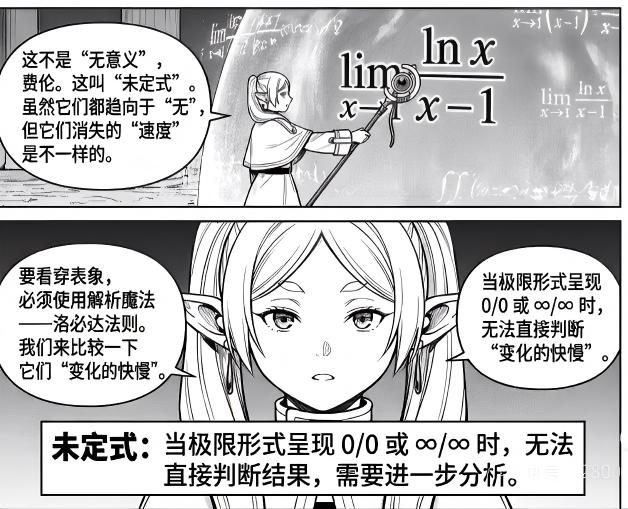
\includegraphics[width=0.7\linewidth]{figure/C6/222}
\end{center}
L'Hospital 法则用于处理函数极限的待定型$(\dfrac{\star}{\infty},\dfrac{0}{0})$
\begin{definition}
	(L'Hospital 法则)设 $f(x), g(x) \in D(a,a+d]$， $g'(x) \neq 0$.且下列条件之一成立：
	
	1.$\lim\limits_{x \to a^+} f(x) = \lim\limits_{x \to a^+} g(x) = 0$
	
	2.$	\lim\limits_{x \to a^+} g(x) = \pm \infty \text{ 或 } \infty$
	
	则有
	\[
	\lim_{x \to a^+} \frac{f(x)}{g(x)} = \lim_{x \to a^+} \frac{f'(x)}{g'(x)}
	\]
	
	
\end{definition}
注：此结论对以下极限行为均有效：
\[
x \to a^+, x \to a^-, x \to a, x \to \infty, x \to -\infty, x \to +\infty
\]

在相应的邻域内，有各自的洛必达法则成立.这里以 $x \to a^+$ 为例.
\begin{proof}
	先考虑 $\lim\limits_{x \to a^+} \dfrac{f'(x)}{g'(x)}$ 存在且有限的情况.设$\lim\limits_{x \to a^+} \dfrac{f'(x)}{g'(x)}=A$
	
	若满足情况1，令
	\[
	\ \widetilde{f}(x) = \begin{cases}
		0 & x = a, \\
		f(x) & x \in (a, a+d],
	\end{cases}
	\quad
	\widetilde{g}(x) = \begin{cases}
		0 & x = a, \\
		g(x) & x \in (a, a+d].
	\end{cases}
	\]
	
	$\widetilde{f}, \widetilde{g}\in C(a, a+d]$, 且对于 $x \in (a, a+d]$, $\widetilde{f}'(x) = f'(x)$, $\widetilde{g}'(x) = g'(x)$.
	
	由 $g'(x) \neq 0$ 及 Rolle 定理，$g(x)$ 在 $(a, a+d]$ 上至多有一个零点.
	必要时缩小 $d$，可设 $g(x) \neq 0$ 对一切 $x \in (a, a+d]$ 成立，从而 Cauchy 中值定理的条件满足.
	
	由 $\widetilde{f}(a) = \widetilde{g}(a) = 0$，对于 $x \in (a, a+d]$，
	\[
	\frac{f(x)}{g(x)} = \frac{\widetilde{f}(x) - \widetilde{f}(a)}{\widetilde{g}(x) - \widetilde{g}(a)}
	\]
	
	由 Cauchy 中值定理，$\exists \xi \in (a, x)$, 使得
	\[
	\frac{f(x)}{g(x)} = \frac{\widetilde{f}(x) - \widetilde{f}(a)}{\widetilde{g}(x) - \widetilde{g}(a)} = \frac{\widetilde{f}'(\xi)}{\widetilde{g}'(\xi)} = \frac{f'(\xi)}{g'(\xi)}
	\]
	
	当 $x \to a^+$ 时，$\xi \to a^+$，故
	\[
	\lim_{x \to a^+} \frac{f(x)}{g(x)} = \lim_{x \to a^+} \frac{f'(\xi)}{g'(\xi)}
	\]
	
	情况 2
	
	取 $x_0 \in(a, a+d]$ 且 $x_0$ 充分靠近 $a$ ．
	$$
	\begin{aligned}
		&\frac{f(x)}{g(x)}=\frac{f(x)-f\left(x_0\right)}{g(x)}+\frac{f\left(x_0\right)}{g(x)}=\frac{f(x)-f\left(x_0\right)}{g(x)-g\left(x_0\right)} \cdot \frac{g(x)-g\left(x_0\right)}{g(x)}+\frac{f\left(x_0\right)}{g(x)} \\
		&\frac{f(x)}{g(x)}-A=\left[\frac{f(x)-f\left(x_0\right)}{g(x)-g\left(x_0\right)}-A\right]\left(1-\frac{g\left(x_0\right)}{g(x)}\right)+A\left(1-\frac{g\left(x_0\right)}{g(x)}\right)+\frac{f\left(x_0\right)}{g(x)}-A \\
		&\left|\frac{f(x)}{g(x)}-A\right| \leqslant\left|\frac{f(x)-f\left(x_0\right)}{g(x)-g\left(x_0\right)}-A\right|\left|1-\frac{g\left(x_0\right)}{g(x)}\right|+\left|\frac{f\left(x_0\right)-A g\left(x_0\right)}{g(x)}\right|\quad(*)
	\end{aligned}
	$$
	
	$\exists \xi $介于$x, x_0$ 之间，使得
	\[
	\frac{f(x) - f(x_0)}{g(x) - g(x_0)} = \frac{f'(\xi)}{g'(\xi)}
	\]
	
	当 $x_0 \to a^+,x \to a^+$, $\xi \to a^+$, 由 $\lim\limits_{x \to a^+} \dfrac{f'(x)}{g'(x)} = A$，$\forall \varepsilon > 0$, $\exists \delta > 0$，当 $x \in (a, a+\delta)$ 时，
	\[
	\left|\frac{f'(x)}{g'(x)} - A\right| < \varepsilon
	\]
	
	取 $x \in (a, a+\delta)$，则 $\xi \in (a, a+\delta) \subset (a, a+d)$，
	\[
	\left|\frac{f'(\xi)}{g'(\xi)} - A\right| < \eps
	\]
	
	代入 $(*)$，
	\[
	\left|\frac{f(x)}{g(x)} - A\right| \leqslant 
	\eps \left|1 - \frac{g(x_0)}{g(x)}\right|+\left|\frac{f(x_0) - A g(x_0)}{g(x)}\right|
	\]
	
	对上述 $x_0$，
	\[
	\lim_{x \to a^+} \left(1 - \frac{g(x_0)}{g(x)}\right) = 1, \quad \lim_{x \to a^+} \frac{f(x_0) - A g(x_0)}{g(x)} = 0
	\]
	
	$\exists \rho$ 使得 $0 < \rho < \delta$，使得 $x \in (a, a+\rho)$ 时，
	\[
	\left|1 - \frac{g(x_0)}{g(x)}\right| < 1 + \frac{\eps}{2}, \quad \left|\frac{f(x_0) - A g(x_0)}{g(x)}\right| < \frac{\eps}{2}
	\]
	
	则
	\[
	\left|\frac{f(x)}{g(x)} - A\right| < \eps \left(1 + \frac{\eps}{2}\right) + \frac{\eps}{2}
	\]
	
	故
	\[
	\lim_{x \to a^+} \frac{f(x)}{g(x)} = A
	\]
	
	下面考虑 $\lim\limits_{x \to a^+} \dfrac{f'(x)}{g'(x)} = \pm\infty$ 的情况.从 $+\infty$ 为例.
	
	情况1: $\lim\limits_{x \to a^+} f(x) = \lim\limits_{x \to a^+} g(x) = 0$，考虑 $(a, a+d]$.
	
	令
	\[
	\ \widetilde{f}(x) = \begin{cases}
		0 & x = a, \\
		f(x) & x \in (a, a+d],
	\end{cases}
	\quad
	\widetilde{g}(x) = \begin{cases}
		0 & x = a, \\
		g(x) & x \in (a, a+d].
	\end{cases}
	\]
	
	由 $\lim\limits_{x \to a^+} \dfrac{f'(x)}{g'(x)} = +\infty$，$\forall G > 0$, $\exists \delta > 0$，$\forall x \in (a, a+\delta)$，使
	\[
	\frac{f'(x)}{g'(x)} > G
	\]
	
	由 Cauchy 中值定理，$\exists \xi \in (a, a+\delta)$ 使
	\[
	\frac{f(x)}{g(x)} = \frac{\widetilde{f}(x) - \widetilde{f}(a)}{\widetilde{g}(x) - \widetilde{g}(a)} = \frac{f'(\xi)}{g'(\xi)} > G
	\]
	
	故
	\[
	\lim_{x \to a^+} \frac{f(x)}{g(x)} = +\infty
	\]
	
	情况2: 设 $\lim\limits_{x \to a^+} g(x) = \infty$.任取 $x_0 \in (a, a+\delta)$, $\delta_1 \in (0, x_0 - a)$.使得当 $x \in (a, a+\delta_1)$ 时
	
	\[
	\max \left\{ \left|\dfrac{g(x_0)}{g(x)}\right|, \left|\dfrac{f(x_0)}{g(x)}\right|\right\} \leqslant \frac{1}{2}
	\]
	
	由
	\[
	\frac{f(x)}{g(x)} = \left[1 - \frac{g(x_0)}{g(x)}\right] \frac{f(x) - f(x_0)}{g(x) - g(x_0)} + \frac{f(x_0)}{g(x)}	= \left[1 - \frac{g(x_0)}{g(x)}\right] \frac{f'(\xi)}{g'(\xi)} + \frac{f(x_0)}{g(x)}
	\]
	对 $x \in (a, a+\delta_1)$ 时
	\[
	\left|\frac{f(x)}{g(x)}\right| \geqslant \frac{1}{2}(G + 1) - \frac{1}{2} = \frac{G}{2}
	\]
	
	故
	\[
	\lim_{x \to a^+} \frac{f(x)}{g(x)} = +\infty
	\]
	
\end{proof}

%
% 第8节：Taylor公式
% !TEX root = ../../../main.tex
% 所属：第一部分：单变量分析学 / 第7章：微分法
% 节：7.8 Taylor公式
% 正文按原文件顺序保存；由 ../chapter7.tex 调用。
\section{Taylor公式}
\begin{theorem}(带 Peano 余项的 Taylor 公式)
	设 $f(x)$ 在 $x = x_0$ 处有 $n$ 阶导数.则存在 $x_0$ 的邻域 $O(x_0, \delta)$，在 $O(x_0, \delta)$ 上，
	\[
	f(x) = f(x_0) + f'(x_0)(x-x_0) + \frac{1}{2!} f''(x_0)(x-x_0)^2 + \cdots + \frac{1}{n!} f^{(n)}(x_0)(x-x_0)^n + r_n(x)
	\]
	
	其中，$r_n(x) = o((x-x_0)^n)$，称为 Peano 余项.
	
	
\end{theorem}
\begin{proof}
	设
	\[
	r_n(x) = f(x) - \left[f(x_0) + f'(x_0)(x-x_0) + \cdots + \frac{1}{n!} f^{(n)}(x_0)(x-x_0)^n\right]
	\]
	下证 $r_n(x) = o((x-x_0)^n)$，也即
	\[
	\lim_{x \to x_0} \frac{r_n(x)}{(x-x_0)^n} = 0
	\]
	对 $n$ 用归纳法. $n=1$ 时，由导数的定义，
	\[
	f(x) = f(x_0) + f'(x_0)(x-x_0) + o(x-x_0),
	\]
	即 $r_1(x) = o(x-x_0)$，成立.
	
	假设结论对 $n$ 成立. 设 $f$ 在 $x_0$ 有 $n+1$ 阶导数，则 $f'$ 在 $x_0$ 有 $n$ 阶导数.
	将 $f$ 写成 $f(x)=P_{n+1}(x)+r_{n+1}(x)$，其中 $P_{n+1}$ 是 $n+1$ 次 Taylor 多项式.
	
	注意到 $r_{n+1}(x_0) = r_{n+1}'(x_0) = \cdots = r_{n+1}^{(n)}(x_0) = 0$，
	且 $r_{n+1}^{(n+1)}(x_0) = 0$. 反复应用 Cauchy 中值定理：
	\[
	\frac{r_{n+1}(x)}{(x-x_0)^{n+1}}
	= \frac{r_{n+1}'(\xi_1)}{(n+1)(\xi_1-x_0)^n}
	= \cdots
	= \frac{r_{n+1}^{(n)}(\xi_n)}{(n+1)!\,(\xi_n-x_0)},
	\]
	其中 $\xi_k$ 介于 $x_0$ 与 $\xi_{k-1}$ 之间（$\xi_0 = x$）.
	最后一步，
	\[
	\frac{r_{n+1}^{(n)}(\xi_n)}{\xi_n-x_0}
	= \frac{r_{n+1}^{(n)}(\xi_n) - r_{n+1}^{(n)}(x_0)}{\xi_n-x_0}
	\to r_{n+1}^{(n+1)}(x_0) = 0 \quad (\xi_n\to x_0).
	\]
	故 $r_{n+1}(x) = o((x-x_0)^{n+1})$，归纳完成.
\end{proof}
\begin{theorem}(带 Lagrange 余项的 Taylor 公式)
	设 $f(x) \in D^n[a, b]\cap D^{n+1}(a, b)$，任取 $ x_0 \in (a,b)$，$\exists \xi \in (a, b)$ 介于 $x$ 与 $x_0$ 之间，使得
	\[
	f(x) = f(x_0) + f'(x_0)(x-x_0) + \cdots + \frac{1}{n!} f^{(n)}(x_0)(x-x_0)^n + \frac{f^{(n+1)}(\xi)}{(n+1)!}(x-x_0)^{n+1}
	\]
	$r_n(x)=\dfrac{f^{(n+1)}(\xi)}{(n+1)!}(x-x_0)^{n+1}$称为Lagrange余项
\end{theorem}
\begin{proof}
	考虑辅助函数
	\[
	G(t) = f(x) - \sum_{k=0}^n \frac{1}{k!} f^{(k)}(t)(x-t)^k \quad \text{和} \quad H(t) = (x-t)^{n+1}.
	\]
	
	那么定理的结论（即需要证明的）是
	\[
	G(x_0) = \frac{f^{(n+1)}(\xi)}{(n+1)!} H(x_0).
	\]
	
	不妨设 $x_0 < x$（$x < x_0$ 时证明类似）.则 $G(t)$ 和 $H(t)$ 在 $[x_0, x]$ 上连续，在 $(x_0, x)$ 上可导，且
	
	\[\begin{aligned}
		G'(t) =& -[f'(t) + (-f'(t)) + f''(t)(x-t) + (-f''(t))(x-t)+ \frac{1}{2!} f'''(t)(x-t)^2 + \cdots\\&-\frac{1}{(n-1)!} f^{(n)}(t)(x-t)^{n-1} + \frac{f^{(n+1)}(t)}{n!}(x-t)^n]\\
		=&-\frac{1}{n!} f^{(n+1)}(t)(x-t)^n
	\end{aligned}\]
	
	\[
	H'(t) = -(n+1)(x-t)^n.
	\]
	
	显然 $H'(t)$ 在 $(x_0, x)$ 上不等于零.因为 $G(x) = H(x) = 0$，由 Cauchy 中值定理可得
	\[
	\frac{G(x_0)}{H(x_0)} = \frac{G(x) - G(x_0)}{H(x) - H(x_0)} = \frac{G'(\xi)}{H'(\xi)} = \frac{f^{(n+1)}(\xi)}{(n+1)!}, \quad \xi \in (x_0, x),
	\]
	
	由此 $G(x_0) = \dfrac{f^{(n+1)}(\xi)}{(n+1)!} H(x_0)$.
\end{proof}
\begin{corollary}(Maclaurin 公式)
	在 $x_0=0$ 时的 Taylor 公式，即为 Maclaurin 公式，
	$$
	f(x) = f(0) + f'(0)x + \frac{1}{2!} f''(0)x^2 + \cdots + \frac{1}{n!} f^{(n)}(0)x^n + r_n(x)
	$$
	
	其中余项
	$$
	r_n(x) = o(x^n) \quad \text{或} \quad \frac{f^{(n+1)}(\xi)}{(n+1)!} x^{n+1} \quad (\xi \text{ 介于 } 0 \text{ 与 } x \text{ 之间})
	$$
\end{corollary}
利用上面的公式，代入一些函数，可以直接得到以下函数的Maclaurin展开
\begin{proposition}
	在$x=0$的邻域内，有
	
	1.
	\[
	e^x = 1 + x + \frac{1}{2!}x^2 + \frac{1}{3!}x^3 + \cdots + \frac{1}{n!}x^n + r_n(x)
	\]
	
	推论：
	\[
	\lim_{n \to \infty} \left(1 + 1 + \frac{1}{2!} + \cdots + \frac{1}{n!}\right) = e
	\]
	
	2.
	\[
	\cos x = 1 - \frac{1}{2!}x^2 + \frac{1}{4!}x^4 - \frac{1}{6!}x^6 + \cdots + \frac{(-1)^n}{(2n)!}x^{2n} + r_{2n+1}(x)
	\]
	
	\[
	\sin x = x - \frac{1}{3!}x^3 + \frac{1}{5!}x^5 - \frac{1}{7!}x^7 + \cdots + \frac{(-1)^n}{(2n+1)!}x^{2n+1} + r_{2n+2}(x)
	\]
	
	\[
	\tan x = x + \frac{1}{3}x^3 + \frac{2}{15}x^5 + \frac{17}{315}x^7 + r_9(x)
	\]
	
	3. 对于 $f(x) = (1+x)^\alpha$, $\alpha \in \mathbb{R}$,
	
	\[\begin{aligned}
		f(x) &= (1+x)^\alpha = 1 + C_\alpha^1 x + C_\alpha^2 x^2 + \cdots + C_\alpha^{\alpha-1} x^{\alpha-1} + x^\alpha\\
		&\Rightarrow C_\alpha^0 + C_\alpha^1 x + \cdots + C_\alpha^n x^n + r_n(x) \quad (n < \alpha \text{ 时})\\
		&\Rightarrow C_\alpha^0 + C_\alpha^1 x + \cdots + C_\alpha^{\alpha-1} x^{\alpha-1} + x^\alpha \quad (n > \alpha \text{ 时})
	\end{aligned}	\]
	
	
	若$ \alpha \notin \mathbb{Z}_+$, $\forall k \in \mathbb{R}$, $C_\alpha^k \neq 0$,
	\[
	(1+x)^\alpha = 1 + \alpha x + \frac{\alpha(\alpha-1)}{2!}x^2 + \cdots + \frac{\alpha(\alpha-1)\cdots(\alpha-n+1)}{n!}x^n + r_n(x)
	\]
	
	当 $\alpha = -1$ 时，
	\[
	\frac{1}{1+x} = 1 - x + x^2 - x^3 + x^4 - \cdots + (-1)^n x^n + r_n(x)\quad(*)
	\]
	
	对于 $\alpha = \dfrac{1}{2}$，
	\[
	\sqrt{1+x} = 1 + \frac{1}{2}x - \frac{1}{2 \cdot 4}x^2 + \frac{1 \cdot 3}{2 \cdot 4 \cdot 6}x^3 - \cdots + (-1)^{n-1} \frac{(2n-3)!!}{(2n)!!}x^n + r_n(x)
	\]
	
	系数为
	\[
	\begin{cases}
		\dfrac{1}{2} & \text{当 } k=1, \\
		(-1)^{k-1} \dfrac{(2k-3)!!}{(2k)!!} & \text{当 } k > 1.
	\end{cases}
	\]
	
	对于 $\alpha = -\dfrac{1}{2}$，
	\[
	\frac{1}{\sqrt{1+x}} = 1 - \frac{1}{2}x + \frac{1 \cdot 3}{2 \cdot 4}x^2 - \frac{1 \cdot 3 \cdot 5}{2 \cdot 4 \cdot 6}x^3 + \cdots + (-1)^n \frac{(2n-1)!!}{(2n)!!}x^n + r_n(x)
	\]
	
	系数为
	\[
	(-1)^n \frac{(2n-1)!!}{(2n)!!}.
	\]
	
	对于 $(*)$，分别代入$-x,x^2,-x^2$：
	\[
	\frac{1}{1-x} = 1 + x + x^2 + x^3 + \cdots + x^n + r_n(x)
	\]
	\[
	\frac{1}{1+x^2} = 1 - x^2 + x^4 - x^6 + \cdots + (-1)^n x^{2n} + r_{2n}(x)
	\]
	\[
	\frac{1}{1-x^2} = 1 + x^2 + x^4 + \cdots + x^{2n} + r_{2n}(x)
	\]
\end{proposition}
这里介绍一条定理，用于计算一些函数的展开
\begin{proposition}
	在$x_0$的某个邻域内，$f(x)\in D^{n+2}$，则它的$n+1$次Taylor多项式的导数恰为$f'(x)$的$n$次Taylor 展开
\end{proposition}
\begin{proof}
	设
	\[
	f(x) = f(x_0) + f'(x_0)(x-x_0) + \cdots + \frac{1}{(n+1)!} f^{(n+1)}(x_0)(x-x_0)^{n+1} + r_{n+1}(x)
	\]
	
	\[
	f'(x) = P_{n+1}(x) = f'(x_0) + f''(x_0)(x-x_0) + \cdots + \frac{1}{n!} f^{(n)}(x_0)(x-x_0)^n + r'_{n+1}(x)
	\]
	
	这意味着存在 $g_n(x)$ 使得
	\[
	\lim_{x \to x_0} \frac{r'_{n+1}(x)}{g_n(x)} = 1
	\]
	
	\[
	f'(x) = f'(x_0) + f''(x_0)(x-x_0) + \cdots + \frac{1}{n!} f^{(n)}(x_0)(x-x_0)^n + g_n(x)
	\]
	
	且
	\[
	\lim_{x \to x_0} g_n(x) = 0
	\]
\end{proof}
\begin{proposition}
	1. 已知
	\[
	\frac{1}{1+x} = 1 - x + x^2 - x^3 + \cdots + (-1)^n x^n + r_n(x)
	\]
	
	设
	\[
	\ln(1+x) = a_0 + a_1 x + \cdots + a_n x^n + r_n(x)
	\]
	
	对 $\ln(1+x)$ 求导，
	\[\begin{aligned}
		(\ln(1+x))' &= a_1 + 2a_2 x + \cdots + n a_n x^{n-1} + r_{n-1}(x)\\&= \frac{1}{1+x} = 1 - x + x^2 - \cdots + (-1)^n x^n + r_{n-1}(x)
	\end{aligned}\]
	得
	\[
	\ln(1+x) = x - \frac{1}{2}x^2 + \frac{1}{3}x^3 - \cdots + (-1)^{n-1} \frac{1}{n} x^n + r_n(x)
	\]
	
	同理
	\[
	\ln(1-x) = -x - \frac{1}{2}x^2 - \frac{1}{3}x^3 - \cdots - \frac{1}{n}x^n + r_n(x)
	\]
	2. 由 $(\tan^{-1} x)' = \dfrac{1}{1+x^2} = 1 - x^2 + x^4 - x^6 + \cdots + (-1)^n x^{2n} + r_{2n}(x)$，
	得
	\[
	\tan^{-1} x = x - \frac{1}{3}x^3 + \frac{1}{5}x^5 - \frac{1}{7}x^7 + \cdots + (-1)^n \frac{1}{2n+1} x^{2n+1} + r_{2n+1}(x)
	\]
	
	类似地，
	\[
	\sin^{-1} x = x + \frac{1}{2} \cdot \frac{1}{3} x^3 + \frac{1 \cdot 3}{2 \cdot 4} \cdot \frac{1}{5} x^5 + \cdots + \frac{(2n-1)!!}{(2n)!!} \cdot \frac{1}{2n+1} x^{2n+1} + r_{2n}(x)
	\]
	
	而
	\[
	\cos^{-1} x = \frac{\pi}{2} - \sin^{-1} x
	\]
	
	3. 对于 $a^x = e^{x \ln a}$，
	\[
	a^x = 1 + x \ln a + \frac{1}{2!} (x \ln a)^2 + \cdots + \frac{1}{n!} (x \ln a)^n + r_n(x)
	\]
	
	4.
	\[
	\ln \left(\frac{1+x}{1-x}\right) = 2 \left(x + \frac{1}{3}x^3 + \cdots + \frac{1}{2n+1}x^{2n+1}\right) + r_{2n+1}(x)
	\]
	
	5.
	\[
	\cosh x = 1 + \frac{1}{2!}x^2 + \frac{1}{4!}x^4 + \cdots + \frac{1}{(2n)!}x^{2n} + r_{2n}(x)
	\]
	
	\[
	\sinh x = x + \frac{1}{3!}x^3 + \frac{1}{5!}x^5 + \cdots + \frac{1}{(2n-1)!}x^{2n-1} + r_{2n-1}(x)
	\]
\end{proposition}

%
% 第9节：一些应用
% !TEX root = ../../../main.tex
% 所属：第一部分：单变量分析学 / 第7章：微分法
% 节：7.9 一些应用
% 正文按原文件顺序保存；由 ../chapter7.tex 调用。
\section{一些应用}
\begin{definition}
	函数 $f(x)$ 在无穷区间有定义，若 $f(x)$ 的斜近线为 $y = ax + b$，则满足
	\[
	\lim_{x \to +\infty} \left[ f(x) - (ax + b) \right] = 0
	\]
	
	易知
	\[
	\lim_{x \to +\infty} \frac{f(x)}{x} = a, \quad \lim_{x \to +\infty} \left[ f(x) - ax \right] = b
	\]
	
	水平渐近线是斜渐近线 $a=0$ 时的退化形式
	
	垂直渐近线是 $x=a$.满足
	\[
	\lim_{x \to a} f(x) = +\infty, -\infty \text{ 或 } \infty
	\]
	
	此处可 $x \to a$，$x \to a^+$，$x \to a^-$.
\end{definition}
另外一种应用是

\textbf{极值点的判定}
	
	函数 $f(x)$ 在区间 $(a, b)$ 上有定义，有以下两种情况：
	
	1. $f(x)$ 在 $x_0$ 处不可导：用极值点定义判别.
	
	2. $f(x)$ 在 $x_0$ 处可导，且 $f'(x_0) = 0$，进一步判别：
	
	若存在 $\delta > 0$，使得 $f(x)$ 在区间 $(x_0 - \delta, x_0 + \delta)$ 内有定义（否则使用极值点的定义）：
	
	(1) 二阶导数不存在：
	
	(i) $\forall x \in (x_0 - \delta, x_0), f'(x)\geqslant0$ 且 $\forall x \in (x_0, x_0 + \delta), f'(x)\leqslant0$ 时，$x_0$ 是极大值点
	
	(ii) $\forall x \in (x_0 - \delta, x_0), f'(x)\leqslant0$ 且 $\forall x \in (x_0, x_0 + \delta), f'(x)\geqslant0$ 时，$x_0$ 是极小值点
	
	(iii) $(x_0 - \delta,x_0),(x_0, x_0 + \delta)$ 上$f'(x)$同号，则不存在极值点
	
	(2) 二阶导数存在：
	
	在 $(x_0 - \delta, x_0 + \delta)$ 内，
	\[ f(x) = f(x_0) + f'(x_0)(x-x_0) + \frac{1}{2!} f''(x_0)(x-x_0)^2 \]
	
	\[ f(x) - f(x_0) = \frac{1}{2!} f''(x_0)(x-x_0)^2 \]
	
	当 $f''(x_0) > 0$ 时，$x_0$ 为严格极小值点，
	
	当 $f''(x_0) < 0$ 时，$x_0$ 为严格极大值点.

\subsection*{绘制图像的一般步骤}

导数为我们提供了系统绘制函数图像的工具。借助一阶导数和二阶导数，我们可以确定函数的单调区间、极值点、凹凸性、拐点，并结合渐近线等信息，勾勒出函数的大致图像。



绘制函数 $y=f(x)$ 图像的步骤如下：

\begin{enumerate}
	\item \textbf{确定定义域}：找出 $f(x)$ 的自然定义域，并关注间断点。
	\item \textbf{奇偶性与周期性}：判断 $f(x)$ 是否具有奇偶性或周期性，可简化后续分析。
	\item \textbf{一阶导数 $f'(x)$}：求出 $f'(x)$ 及其零点（驻点）和不存在点，利用 $f'(x)$ 的符号划分单调区间，并用第一或第二充分条件判定极值。
	\item \textbf{二阶导数 $f''(x)$}：求出 $f''(x)$ 及其零点和不存在点，确定凹凸区间与拐点。
	\item \textbf{渐近线}：计算水平渐近线、垂直渐近线和斜渐近线。
	\item \textbf{关键点与辅助点}：计算驻点、拐点、与坐标轴的交点等关键位置的函数值，必要时补充若干辅助点。
	\item \textbf{描点连线}：在坐标系中标出所有关键点，结合单调性、凹凸性和渐近线，平滑地连接成函数图像。
\end{enumerate}



\begin{example}
	绘制函数 $f(x)=\dfrac{x^3}{x^2-1}$ 的图像。
\end{example}

\begin{proof}[解]
	\textbf{1. 定义域}：分母 $x^2-1\neq0$，故定义域为 $(-\infty,-1)\cup(-1,1)\cup(1,+\infty)$。

	\textbf{2. 奇偶性}：
	\[
	f(-x)=\frac{(-x)^3}{(-x)^2-1}=-\frac{x^3}{x^2-1}=-f(x)
	\]
	$f(x)$ 为奇函数，图像关于原点对称。

	\textbf{3. 一阶导数}：
	\[
	f'(x)=\frac{3x^2(x^2-1)-x^3\cdot 2x}{(x^2-1)^2}=\frac{x^2(x^2-3)}{(x^2-1)^2}
	\]
	令 $f'(x)=0$，得 $x=0$，$x=\pm\sqrt{3}$。

	单调性分析：

	\begin{center}
		\begin{tabular}{c|ccccccccc}
			$x$ & $(-\infty,-\sqrt{3})$ & $-\sqrt{3}$ & $(-\sqrt{3},-1)$ & $(-1,0)$ & $0$ & $(0,1)$ & $(1,\sqrt{3})$ & $\sqrt{3}$ & $(\sqrt{3},+\infty)$ \\
			\hline
			$f'(x)$ & $+$ & $0$ & $-$ & $-$ & $0$ & $-$ & $-$ & $0$ & $+$ \\
			$f(x)$ & $\nearrow$ & 极大 & $\searrow$ & $\searrow$ & 拐点 & $\searrow$ & $\searrow$ & 极小 & $\nearrow$
		\end{tabular}
	\end{center}

	极大值 $f(-\sqrt{3})=-\dfrac{3\sqrt{3}}{2}$，极小值 $f(\sqrt{3})=\dfrac{3\sqrt{3}}{2}$。

	\textbf{4. 二阶导数}：
	\[
	f''(x)=\frac{2x(x^2+3)}{(x^2-1)^3}
	\]
	令 $f''(x)=0$，得 $x=0$。

	凹凸性分析：

	\begin{center}
		\begin{tabular}{c|ccccc}
			$x$ & $(-\infty,-1)$ & $(-1,0)$ & $0$ & $(0,1)$ & $(1,+\infty)$ \\
			\hline
			$f''(x)$ & $-$ & $+$ & $0$ & $-$ & $+$ \\
			$f(x)$ & 上凸 & 下凸 & 拐点 & 上凸 & 下凸
		\end{tabular}
	\end{center}

	拐点 $(0,0)$。

	\textbf{5. 渐近线}：
	\[
	\lim_{x\to\pm 1^{\mp}}f(x)=\infty,\quad \lim_{x\to\pm 1^{\pm}}f(x)=\mp\infty
	\]
	$x=-1$ 和 $x=1$ 为垂直渐近线。

	\[
	a=\lim_{x\to\infty}\frac{f(x)}{x}=\lim_{x\to\infty}\frac{x^2}{x^2-1}=1
	\]
	\[
	b=\lim_{x\to\infty}[f(x)-ax]=\lim_{x\to\infty}\frac{x}{x^2-1}=0
	\]
	$y=x$ 为斜渐近线（当 $x\to+\infty$ 和 $x\to-\infty$ 时均成立）。

	\textbf{6. 辅助点}：
	\[
	f(0)=0,\quad f\left(\pm\frac{1}{2}\right)=\mp\frac{1}{6},\quad f(\pm 2)=\pm\frac{8}{3}
	\]

	\textbf{7. 绘制图像}：综合以上信息，先画出三条渐近线 $x=-1$、$x=1$ 和 $y=x$，再标出极值点与拐点，最后按照单调性和凹凸性平滑连接即可。
\end{proof}

上述例子展示了利用导数绘制函数图像的一般流程。在更复杂的情形中，若函数含有指数、对数或三角函数，仍需遵循相同的分析框架，逐项确定定义域、单调性、凹凸性和渐近线，最后综合成图。
%

%% ===== 第一部分：单变量分析学 / 第8章：Riemann积分 =====
% !TEX root = ../../main.tex
\setchapterimage{figure/chapter8封面图.png}
\setchapterintro{这一章讲Riemann积分，囊括了不定积分,定积分与反常积分等内容，后面三章会分别讲这几个部分的一些命题和习题}
\chapter{Riemann积分}
% 第1节：不定积分
% !TEX root = ../../../main.tex
% 所属：第一部分：单变量分析学 / 第8章：Riemann积分
% 节：8.1 不定积分
% 正文按原文件顺序保存；由 ../chapter8.tex 调用。
\section{不定积分}
\begin{definition}
	设 \( y = f(x) \) ,在某个区间上,\( F'(x) = f(x) \),则称 \( F(x) \) 是 \( f(x) \) 的一个原函数或反导数,\( y = F(x) + \text{const} \) 是 \( y = f(x) \) 的原函数
	
\end{definition}
\begin{proposition}\label{原函数只差}
	在某区间上,若 \( f(x) \) 的任意两个原函数之差为常数.也即,设 \( F_1(x) \)、\( F_2(x) \) 为 \( f(x) \) 的原函数,则
	\[
	F_1(x) - F_2(x) = C
	\]
	
	
	
\end{proposition}
\begin{proof}
	\( F_1'(x) = F_2'(x) = f(x) \),在区间 \( I \) 上,令
	\[
	F(x) = F_1(x) - F_2(x)
	\]
	$
	F'(x) \equiv 0, \forall x \in I, \text{由 Rolle 定理,} F(x) = \text{Const.}$
\end{proof}
\begin{definition}
	在某区间上, \( f(x) \) 的不定积分定义为其所有原函数构成的集合,记作
	\[
	\int f(x) \dd x := \{ F(x) : F'(x) = f(x), \, x \in I \}
	\]
	
	由\ref{原函数只差} 等价于
	\[
	\int f(x) \dd x = \{ F(x) + C : \text{任意} F'(x) = f(x) \}
	\]
	
	为便于起见,记做
	\[
	\int f(x) \dd x = F(x) + C\]
	
\end{definition}
微分算子$\dd$与不定积分算子$\int$是一对逆运算,也就是说
$$\dd(\int f(x)\dd x)=f(x)\dd x\text{即}\dfrac{\dd}{\dd x}(\int f(x)\dd x)=f(x)$$
与$$\int\dd F(x)=F(x)+C$$成立

利用导数的性质,我们可以得到相应的积分的性质

利用导数的线性性质,有
\begin{proposition}
	在某区间$I$上, \( f(x) \),\( g(x) \) 的原函数都存在,则 \(\forall \, k_1, k_2 \in \mathbb{R}\),函数 \(k_1 f(x) + k_2 g(x)\) 的原函数也存在,且有
	\[
	\int [k_1 f(x) + k_2 g(x)] \dd x = k_1 \int f(x) \dd x + k_2 \int g(x) \dd x
	\]
	
\end{proposition}
注：等式两边都是函数族.
\begin{proof}
	设 \( F(x) \) 和 \( G(x) \) 分别是 \( f(x) \) 和 \( g(x) \) 的原函数,应有
	\[
	(k_1 F(x) + k_2 G(x))' = k_1 f(x) + k_2 g(x)
	\]
	
	那么
	\[
	\int (k_1 f(x) + k_2 g(x)) \dd x = k_1 F(x) + k_2 G(x) + C
	\]
	
	且
	\[\begin{aligned}
		k_1 \int f(x) \dd x + k_2 \int g(x) \dd x &= k_1 (F(x) + C_1) + k_2 (G(x) + C_2)\\	&= k_1 F(x) + k_2 G(x) + (k_1 C_1 + k_2 C_2)
	\end{aligned}\]
	
	
	上两式揭示的积分族相同,故
	\[
	\int [k_1 f(x) + k_2 g(x)] \dd x = k_1 \int f(x) \dd x + k_2 \int g(x) \dd x\]
\end{proof}
根据导数的乘法公式我们得到不定积分的分部积分公式
\begin{proposition}
	在某区间上,若有两个可微函数 $u(x), v(x)$,则
	\[
	\int u(x) v'(x) \dd x = u(x) v(x) - \int v(x) u'(x) \dd x
	\]
	经常简写为$$\int u \dd v = uv - \int v \dd u$$
	
\end{proposition}
\begin{proof}
	对 $u, v$ 有
	\[
	\dd(uv) = u \dd v + v \dd u
	\]
	
	两边积分,并移项得
	\[
	\int u \dd v = uv - \int v \dd u
	\]
	
	因此
	\[
	\int u(x) v'(x) \dd x = u(x) v(x) - \int v(x) u'(x) \dd x
	\]
\end{proof}

使用复合函数求导公式,我们得到第一类换元积分法.
\begin{proposition}
	对 $f(x)$,换元 $z = g(x)$,使 $f(x) = \tilde{f}(z )g'(x) = \tilde{f}(g(x)) \cdot g'(x)$.
	
	那么
	\[
	\int f(x) \dd x = \int \tilde{f}(g(x)) g'(x) \dd x = \int \tilde{f}(g(x)) \dd[g(x)] = \tilde{F}(g(x)) + C
	\]
	
	其中,$\tilde{F}(x)$ 为 $\tilde{f}(x)$ 的一个原函数.
\end{proposition}
类似的,有第二类换元积分法
\begin{proposition}
	对 $f(x)$,换元 $x = \varphi(t)$,其中 $\varphi(t)$ 是严格单调且可导,即其逆函数 $\varphi^{-1}$ 存在且可导
	\[\begin{aligned}
		\int f(x) \dd x &= \int f(\varphi(t)) \dd\varphi(t) = \int f(\varphi(t)) \cdot \varphi'(t) \dd t\\
		&= F(t) + C = F(\varphi^{-1}(x)) + C
	\end{aligned}\]
	
\end{proposition}\newpage
利用我们已经有的导数表,我们得到以下常用的积分公式
\begin{proposition}
	初等不定积分表：
	\[\begin{aligned}
		&(1)\int 0 \dd x = C\\
		&(2) \int x^\alpha \dd x = \frac{x^{\alpha+1}}{\alpha+1} + C \quad (\alpha \neq -1)\\
		&(3)\int \sin x \dd x = -\cos x + C\\
		&(4)\int \cos x \dd x = \sin x + C\\
		&(5)\int \sec^2 x \dd x = \tan x + C\\
		&(6)\int \csc^2 x \dd x = -\cot x + C\\
		&(7)\int \tan x \sec x \dd x = \sec x + C\\
		&(8)\int \cot x \csc x \dd x = -\csc x + C\\
		&(9)\int \frac{\dd x}{1-x^2} = \sin^{-1} x + C = -\cos^{-1} x + C\\
		&(10)\int \frac{\dd x}{1+x^2} = \tan^{-1} x + C = -\cot^{-1} x + C\\
		& (11) \int a^x \dd x = \frac{a^x}{\ln a} + C \quad (a > 0, a \neq 1)\\
		&(12) \int e^x \dd x = e^x + C\\
		&(13)\int \frac{1}{x} \dd x = \ln |x| + C\\
		&(14)\int \frac{1}{x \ln a} \dd x = \log_a |x| + C\\
		&(15)\int \sinh x \dd x = \cosh x + C\\
		&(16)\int \cosh x \dd x = \sinh x + C\\
		&(17)\int \text{sech}^2 x \dd x = \tanh x + C\\
		&(18)\int \frac{\dd x}{\sqrt{1+x^2}} = \sinh^{-1} x + C\\
		&(19)\int \frac{\dd x}{\sqrt{x^2-1}} = \cosh^{-1} x + C\\
		&(20)\int \frac{\dd x}{1-x^2} = \tanh^{-1} x + C
	\end{aligned}\]
\end{proposition}
此外还有一条相当好用的公式
\begin{proposition}
	\[\int\dfrac{f'(x)}{f(x)}\dd x=\ln|x|+C\]
\end{proposition}
这是第一类换元积分法的直接应用
%
% 第2节：一些例子,一些应用以及有理函数的积分
% !TEX root = ../../../main.tex
% 所属：第一部分：单变量分析学 / 第8章：Riemann积分
% 节：8.2 一些例子,一些应用以及有理函数的积分
% 正文按原文件顺序保存；由 ../chapter8.tex 调用。
\section{一些例子,一些应用以及有理函数的积分}
\begin{problem}
	计算以下不定积分：
	
	(1) $$\int \sin^2 x \dd x$$
	
	(2)$$\int \frac{(x+\sqrt{x})(x-2\sqrt{x})^2}{\sqrt{x}} \dd x$$
	
	(3) $$\int \frac{x^4}{1+x^2} \dd x$$
\end{problem}
\begin{solution}
	(1) 由于 $\sin^2 x = \dfrac{1}{2}(1 - \cos 2x)$,所以
	\[
	\int \sin^2 x \dd x = \frac{1}{2} \int (1 - \cos 2x) \dd x = \frac{1}{2} x - \frac{1}{2} \int \cos 2x \dd x
	\]
	\[
	= \frac{1}{2} x - \frac{1}{4} \sin 2x + C
	\]
	
	(2) \[\begin{aligned}
		\text{原式} &= \int \dfrac{x^3 - 2x^{5/2} + 4x^{3/2}}{x^{1/2}} \dd x\\& = \int (x^{5/2} - 3x^2 + 4x) \dd x\\
		&= \frac{2}{7} x^{7/2} -  x^3 + 2 x^3 + C
	\end{aligned}\]
	
	
	(3)\[\text{原式}= \int \frac{x^4 + x^2 - x^2}{1 + x^2} \dd x = \int \left(x^2 - 1 + \frac{1}{1+x^2}\right) \dd x= \frac{1}{3} x^3 - x + \tan^{-1} x + C\]  
\end{solution}
\begin{problem}
	(1)\[\int x\cos x\dd x\]
	(2)\[\int x^2e^x\dd x\]
	(3)\[\int\ln x\dd x\]
	(4)\[\int e^x\sin x\dd x\]
\end{problem}
\begin{solution}
	(1) $$\int x \cos x \dd x = \int x \dd\sin x = x \sin x - \int \sin x \dd x = x \sin x + \cos x + C$$
	
	(2)\[\begin{aligned}
		\int x^2 e^x \dd x &= \int x^2 \dd e^x = x^2 e^x - 2 \int x e^x \dd x\\&= x^2 e^x - 2 \int x \dd e^x = x^2 e^x - 2(x e^x - \int e^x \dd x) \\&= x^2 e^x - 2x e^x + 2 e^x + C = (x^2 - 2x + 2)e^x + C
	\end{aligned}\] 
	
	(3) $$\int \ln x \dd x = x \ln x - \int x \dd\ln x = x \ln x - \int x \cdot \frac{1}{x} \dd x = x \ln x - x + C$$
	
	(4) 设 $I = \displaystyle\int e^x \sin x \dd x$,$J = \displaystyle\int e^x \cos x \dd x$,
	\[
	\begin{cases}
		I = \displaystyle\int \sin x \dd e^x = e^x \sin x - \displaystyle\int e^x \cos x \dd x = e^x \sin x - J \\
		J = \displaystyle\int \cos x \dd e^x = e^x \cos x + \displaystyle\int e^x \sin x \dd x = e^x \cos x + I
	\end{cases}
	\]
	解得：
	\[
	I = \frac{1}{2} e^x (\sin x - \cos x) + C, \quad J = \frac{1}{2} e^x (\cos x + \sin x) + C
	\]
\end{solution}
\begin{problem}
	(1)$$\int\frac{\dd x}{x^2+a^2}\text{与}\int \frac{\dd x}{\sqrt{a^2-x^2}}$$
	(2)$$\int\tan x\dd x\text{与}\int\cot x\dd x$$
	(3)$$\int\sec x\dd x\text{与}\int\csc x\dd x$$
	(4)$$\int\frac{\dd x}{\sqrt{x}(1+x)}$$
\end{problem}
\begin{solution}
	(1)
	\[
	\int \frac{\dd x}{x^2 + a^2} = \frac{1}{a} \int \frac{\dd\left(\dfrac{x}{a}\right)}{\left(\dfrac{x}{a}\right)^2 + 1} = \frac{1}{a} \tan^{-1} \frac{x}{a} + C
	\]
	
	\[
	\int \frac{\dd x}{\sqrt{a^2-x^2}} = \int \frac{\dd\left(\dfrac{x}{a}\right)}{1 - \sqrt{\left(\dfrac{x}{a}\right)^2}} = \sin^{-1} \dfrac{x}{a} + C
	\]
	
	(2)
	\[
	\int \tan x \dd x = \int \frac{\sin x}{\cos x} \dd x = -\ln |\cos x| + C
	\]
	
	\[
	\int \cot x \dd x = \int \frac{\cos x}{\sin x} \dd x = \ln |\sin x| + C
	\]
	
	(3)
	\[
	\int \sec x \dd x = \int \frac{\sec x (\sec x + \tan x)}{\sec x + \tan x} \dd x = \ln |\sec x + \tan x| + C
	\]
	
	\[
	\int \csc x \dd x = \int \frac{\csc x (\csc x - \cot x)}{\csc x - \cot x} \dd x = -\ln |\csc x - \cot x| + C
	\]
	
	(4)
	\[
	\int \frac{\dd x}{x \sqrt{1 + x}} = 2 \int \frac{\dd(\sqrt{x})}{1 + (\sqrt{x})^2} = 2 \tan^{-1} \sqrt{x} + C
	\]
\end{solution}
\begin{problem}
	(1)\[\int \sqrt{a^2-x^2}\dd x\]
	(2)\[\int\frac{\dd x}{\sqrt{x^2-a^2}}\text{和}\int\frac{\dd x}{\sqrt{x^2+a^2}}\]
	(3)\[\int \sqrt{x^2+a^2}\dd x\text{和}\int \sqrt{x^2-a^2}\dd x\]
\end{problem}
\begin{solution}
	(1) 设 $x = a \sin \theta$,则 $\dd x = a \cos \theta \dd \theta$,
	\[\begin{aligned}
		\int \sqrt{a^2 - x^2} \dd x &= \int a^2 \cos^2 \theta \dd \theta = a^2 \int \frac{1 + \cos 2\theta}{2} \dd \theta\\
		&= \frac{1}{2} a^2 \theta + \frac{1}{4} a^2 \sin 2\theta + C\\	&= \frac{1}{2} a^2 \sin^{-1} \frac{x}{a} + \frac{1}{2} a^2 \cdot \frac{x}{a^2} \sqrt{a^2 - x^2} + C\\&= \frac{1}{2} x \sqrt{a^2 - x^2} + \frac{a^2}{2} \sin^{-1} \frac{x}{a} + C
	\end{aligned}\]
	(2) 设 $x = a \sec \theta$,则 $\dd x = a \sec \theta \tan \theta \dd \theta$,
	\[\begin{aligned}
		\int \frac{\dd x}{ \sqrt{x^2 - a^2}} &= \int \frac{a \sec \theta \tan \theta \dd \theta}{ a \tan \theta} = \int \sec \theta \dd \theta = \ln |\sec \theta + \tan \theta| + C\\&= \ln \left| \frac{x}{a} + \frac{\sqrt{x^2 - a^2}}{a} \right| + C = \ln \left| x + \sqrt{x^2 - a^2} \right| + C
	\end{aligned}\]
	
	
	同理
	\[
	\int \frac{\dd x}{\sqrt{x^2 + a^2}} = \ln \left| x + \sqrt{x^2 + a^2} \right| + C
	\]
	(3) 考虑 $\displaystyle\int \sqrt{x^2 + a^2} \dd x$：
	
	\[\begin{aligned}
		\int \sqrt{x^2 + a^2} \dd x &= x \sqrt{x^2 + a^2} - \int \frac{x^2}{\sqrt{x^2 + a^2}} \dd x\\& = x \sqrt{x^2 + a^2} + \int \frac{a^2}{\sqrt{x^2 + a^2}} \dd x - \int \sqrt{x^2 + a^2} \dd x
	\end{aligned}\]
	
	移项得：
	\[
	2 \int \sqrt{x^2 + a^2} \dd x = x \sqrt{x^2 + a^2} + a^2 \ln \left| x + \sqrt{x^2 + a^2} \right| + C
	\]
	
	因此：
	\[
	\int \sqrt{x^2 + a^2} \dd x = \frac{1}{2} \left( x \sqrt{x^2 + a^2} + a^2 \ln \left| x + \sqrt{x^2 + a^2} \right| \right) + C
	\]
	
	同理
	\[
	\int \sqrt{x^2 - a^2} \dd x = \frac{1}{2} \left( x \sqrt{x^2 - a^2} - a^2 \ln \left| x + \sqrt{x^2 - a^2} \right| \right) + C
	\]
\end{solution}
这样我们得到基本积分表的下半部分
\begin{proposition}
	(1) $$\int \tan x \dd x = -\ln |\cos x| + C$$
	
	(2) $$\int \cot x \dd x = \ln |\sin x| + C$$
	
	(3) $$\int \sec x \dd x = \ln |\sec x + \tan x| + C$$
	
	(4) $$\int \csc x \dd x = \ln |\csc x - \cot x| + C$$
	
	(5) $$\int \frac{\dd x}{\sqrt{x^2 \pm a^2}} = \ln \left| x + \sqrt{x^2 \pm a^2} \right| + C$$
	
	(6)$$\int \frac{\dd x}{\sqrt{a^2 - x^2}} =  \sin^{-1} \frac{x}{a} + C$$
	
	(7) $$\int \frac{\dd x}{x^2 - a^2} = \frac{1}{2a} \ln \left| \frac{x - a}{x + a} \right| + C$$
	
	(8) $$\int \frac{\dd x}{x^2 + a^2} = \frac{1}{a} \tan^{-1} \frac{x}{a} + C$$
	
	(9) $$\int \sqrt{a^2 - x^2} \dd x = \frac{1}{2} x \sqrt{a^2 - x^2} + \frac{a^2}{2} \sin^{-1} \frac{x}{a} + C$$
	
	(10)$$\int \sqrt{x^2 \pm a^2} \dd x = \frac{1}{2} \left( x \sqrt{x^2 \pm a^2} \pm a^2 \ln \left| x + \sqrt{x^2 \pm a^2} \right| \right) + C$$
\end{proposition}
\begin{problem}计算下列积分
	\begin{enumerate}
		\item[(1)]
		$\displaystyle \int \frac{\dd x}{\sqrt{x^2 + 2\xi x + \eta^2}}$
		
		\item[(2)]
		$\displaystyle \int \frac{ax + b}{\sqrt{x^2 + 2\xi x + \eta^2}} \dd x$
		
		\item[(3)]
		$\displaystyle \int \frac{ax + b}{x^2 + 2\xi x + \eta^2} \dd x$
		
		\item[(4)]
		$\displaystyle \int (ax + b) \sqrt{x^2 + 2\xi x + \eta^2} \dd x$
	\end{enumerate}
	
\end{problem}
\begin{solution}
	(1)\[\int \frac{\dd x}{\sqrt{x^2 + 2\xi x + \eta^2}} = \int \frac{\dd(x + \xi)}{\sqrt{(x + \xi)^2 \pm |\eta^2 - \xi^2|}} = \ln \left| x + \xi + \sqrt{x^2 + 2\xi x + \eta^2} \right| + C\]
	(2)$$\begin{aligned}
		&\int \frac{ax + b}{x^2 + 2\xi x + \eta^2} \dd x
		= \frac{a}{2} \int \frac{\dd(x^2 + 2\xi x + \eta^2)}{x^2 + 2\xi x + \eta^2} + (b - a\xi) \int \frac{\dd x}{(x+\xi)^2+\eta^2-\xi^2} \\
		&= \begin{cases}
			a \ln \left| x + \xi  \right| - \dfrac{b - a\xi}{x+\xi}  + C, & |\xi| =|\eta| \\
			\dfrac{a}{2} \ln \left| x^2 + 2\xi x + \eta^2 \right| + \dfrac{b - a\xi}{\sqrt{\eta^2 - \xi^2}} \arctan\dfrac{x+\xi}{\sqrt{\eta^2-\xi^2}} + C, & |\xi| < |\eta| \\
			\dfrac{a}{2} \ln \left| x^2 + 2\xi x + \eta^2 \right| + \dfrac{b - a\xi}{2\sqrt{\xi^2 - \eta^2}}\ln \left| \dfrac{x + \xi - \sqrt{\xi^2 - \eta^2}}{x + \xi + \sqrt{\xi^2 + \eta^2}} \right|  + C, & |\xi| > |\eta|
		\end{cases}
	\end{aligned}$$
	
	(3)\[\begin{aligned}
		\int \frac{ax + b}{\sqrt{x^2 + 2\xi x + \eta^2}} \dd x
		&= \dfrac{a}{2} \int \frac{\dd(x^2 + 2\xi x + \eta^2)}{\sqrt{x^2 + 2\xi x + \eta^2}} + (b - a\xi) \int \frac{\dd x}{\sqrt{x^2 + 2\xi x + \eta^2}} \\
		&= \sqrt{x^2 + 2\xi x + \eta^2} +(b - a\xi)\ln|x+\xi+ \sqrt{x^2 + 2\xi x + \eta^2}|+C
	\end{aligned}\]
	(4)\[\begin{aligned}
		&\int(ax+b) \sqrt{x^2 + 2\xi x + \eta^2}\dd x\\
		=&\dfrac{a}{2}\int \sqrt{x^2 + 2\xi x + \eta^2}\dd( x^2 + 2\xi x + \eta^2)+(b-a\xi)\int \sqrt{x^2 + 2\xi x + \eta^2}\dd x\\
		=&\dfrac{a}{3} (x^2 + 2\xi x + \eta^2)^{3/2}+\frac{b-a\xi}{2}[(x+\xi) \sqrt{x^2 + 2\xi x + \eta^2}+(\eta^2-\xi^2)\ln|x+\xi+ \sqrt{x^2 + 2\xi x + \eta^2}|]+C
	\end{aligned}\]
\end{solution}
\begin{problem}\label{积分10}
	(1)$$I_n=\int \frac{\dd x}{(x^2+a^2)^n}$$
	(2)\[I_n\int x^ne^x\dd x\]
	(3)\[I_n=\int\cos^nx\dd x\]
\end{problem}
\newpage
\begin{solution}
	(1)对于 $n \geq 2$：
	
	\begin{align*}
		I_n &= \int \frac{\dd x}{(x^2 + a^2)^n} \\
		&= \frac{1}{a^2} \int \frac{\dd x}{(x^2 + a^2)^{n-1}} - \frac{1}{a^2} \int \frac{x^2}{(x^2 + a^2)^n} \dd x \\
		&= \frac{I_{n-1}}{a^2} + \frac{1}{2a^2(n-1)} \int x \, d\left[ \frac{1}{(x^2 + a^2)^{n-1}} \right] \\
		&= \frac{I_{n-1}}{a^2} + \frac{1}{2a^2(n-1)} \left( \frac{x}{(x^2 + a^2)^{n-1}} - \int \frac{\dd x}{(x^2 + a^2)^{n-1}} \right) \\
		&= \frac{I_{n-1}}{a^2} + \frac{1}{2a^2(n-1)} \cdot \frac{x}{(x^2 + a^2)^{n-1}} - \frac{I_{n-1}}{2a^2(n-1)} \\
		&= \frac{2n-3}{2a^2(n-1)} I_{n-1} + \frac{1}{2a^2(n-1)} \cdot \frac{x}{(x^2 + a^2)^{n-1}}
	\end{align*}
	\[\begin{cases}
		I_n= \dfrac{2n-3}{2a^2(n-1)} I_{n-1} + \dfrac{1}{2a^2(n-1)} \cdot \dfrac{x}{(x^2 + a^2)^{n-1}}\\
		I_1=\dfrac{1}{a}\arctan\dfrac{x}{a}+C
	\end{cases}\]
	(2)\[
	I_n = \int x^n e^x \dd x = x^n e^x - \int e^x \dd(x^n) = x^n e^x - n \int x^{n-1} e^x \dd x = x^n e^x - n I_{n-1}
	\]
	
	所以,
	\[
	I_n + n I_{n-1} = x^n e^x
	\]
	
	有初值
	\[
	I_1 = \int x e^x \dd x = x e^x - \int e^x \dd x = (x - 1)e^x + C
	\]
	(3)\[\begin{aligned}
		I_n &= \int \cos^n x \dd x = \int \cos^{n-1} x \cdot \cos x \dd x = \int \cos^{n-1} x \dd(\sin x)\\&= \cos^{n-1} x \sin x + (n-1) \int \sin^2 x \cos^{n-2} x \dd x\\&= \cos^{n-1} x \sin x + (n-1) \int (1 - \cos^2 x) \cos^{n-2} x \dd x\\&	= \cos^{n-1} x \sin x + (n-1) I_{n-2} - (n-1) I_n
	\end{aligned}\]
	整理得：
	
	\[
	I_n = \frac{1}{n} \cos^{n-1} x \sin x + \left(1 - \frac{1}{n}\right) I_{n-2}
	\]
\end{solution}
\begin{problem}(有理函数的积分)
	给定 $P_m(x), Q_n(x) \in \mathbb{R}[x]$,且 $m = \deg P_m$,$n = \deg Q_n$,计算有理函数的积分：
	
	\[
	\int \frac{P_m(x)}{Q_n(x)} \dd x
	\]
\end{problem}
\begin{solution}
	若\( m \geqslant n \),由带余除法 
	
	\[
	P_m(x) = g(x) Q_n(x) + \tilde{P}_m(x)
	\]
	
	所以,
	
	\[
	\frac{P_m(x)}{Q_n(x)} = g(x) + \frac{\tilde{P}_m(x)}{Q_n(x)}, \quad \deg \tilde{P}_m < \deg Q_n
	\]
	
	其中 \( g(x) \) 是多项式,直接积分即可,后面只需考虑 \( n > m \) 的情况,由代数基本定理：
	
	\[
	Q_n(x) = (x - \alpha_1)^{m_1} \cdots (x - \alpha_t)^{m_t} (x^2 + 2\xi_1 x + \eta_1^2)^{n_1} \cdots (x^2 + 2\xi_s x + \eta_s^2)^{n_s}
	\]
	
	其中 \(\alpha_k, \xi_k, \eta_k \in \mathbb{R}\) 且 \(\xi_k^2 - \eta_k^2 < 0\)
	
	对 \(\dfrac{P_m(x)}{Q_n(x)}\) 写出部分分式分解的形式.
	
	每一个一次项：$(x - \alpha_k)^{m_k}$ 对应的展开形式：
	
	\[
	\frac{\lambda_{k1}}{x - \alpha_k} + \frac{\lambda_{k2}}{(x - \alpha_k)^2} + \cdots + \frac{\lambda_{km_k}}{(x - \alpha_k)^{m_k}}
	\]
	
	每一个二次项：$(x^2 + 2\xi_k x + \eta_k^2)^{n_k}$ 对应的展开形式：
	
	\[
	\frac{\mu_{k1}x + \nu_{k1}}{x^2 + 2\xi_k x + \eta_k^2} + \frac{\mu_{k2}x + \nu_{k2}}{(x^2 + 2\xi_k x + \eta_k^2)^2} + \cdots + \frac{\mu_{kn_k}x + \nu_{kn_k}}{(x^2 + 2\xi_k x + \eta_k^2)^{n_k}}
	\]
	
	这些系数可以由待定系数法得出
	
	只需考虑
	
	1.
	\[
	\int \frac{\dd x}{(x - \alpha)^n} =
	\begin{cases}
		\ln |x - \alpha| + C, & n = 1 \\
		\dfrac{1}{1-n} \cdot \dfrac{1}{(x - \alpha)^{n-1}} + C, & n >1
	\end{cases}
	\]
	
	2.\[\begin{aligned}
		\int \frac{\mu x + \nu}{(x^2 + 2\xi x + \eta^2)^n} \dd x &= \frac{\mu}{2} \int \frac{\dd(x^2 + 2\xi x + \eta^2)}{(x^2 + 2\xi x + \eta^2)^n} + (\nu-2\xi) \int \frac{\dd x}{(x^2 + 2\xi x + \eta^2)^n}\\&= \dfrac{\mu}{2(1-n)} \cdot \frac{1}{(x^2 + 2\xi x + \eta^2)^{n-1}} + (\nu-2\xi) I_n
	\end{aligned}\]
	$I_n=\displaystyle\int\dfrac{\dd x}{(x^2+2\xi x+\eta^2)^n}=\displaystyle\int\dfrac{\dd x}{((x+\xi)^2\pm|\eta^2-\xi^2|)^n}$,由\ref{积分10}得
\end{solution}
\begin{problem}
	(可化成有理函数的形式)
	令 \( R(u, v) \)表示关于两个变量 \( u, v \) 的有理函数（分母,分子为二元有理函数）,考虑以下类型的积分：
	
	1.
	\[
	\int R\left(x, \sqrt[n]{\frac{\xi x+\eta}{\mu x+\nu}}\right) \dd x
	\]
	
	2.
	\[
	\int R(\sin x, \cos x) \dd x
	\] 
	
\end{problem}
\begin{solution}
	
	1. 设
	\[
	t = \sqrt[n]{\frac{\xi x+\eta}{\mu x+\nu}}, x = \varphi(t) = \frac{-\nu t^n + \eta}{\mu t^n - \xi}
	\]
	
	则
	\[
	\int R\left(x, \sqrt[n]{\frac{\xi x+\eta}{\mu x+\nu}}\right) \dd x = \int R\left(\frac{-\nu t^n + \eta}{\mu t^n - \xi}, t\right) \varphi'(t) \dd t
	\]
	
	2. 令 \(\tan \dfrac{x}{2} = t\)
	\[
	\sin x = 2 \sin \frac{x}{2} \cos \frac{x}{2} = \frac{2t}{1 + t^2}, \cos x = \frac{1 - t^2}{1 + t^2},  \dd x = \dd(2 \arctan t) = \frac{2 \dd t}{1 + t^2}
	\]
	
	因此
	\[
	\int R(\sin x, \cos x) \dd x = \int R\left(\frac{2t}{1 + t^2}, \frac{1 - t^2}{1 + t^2}\right) \frac{2}{1 + t^2} \dd t
	\]
\end{solution}
\begin{problem}
	\[\int \frac{\dd x}{x(\sqrt[3]{x}-\sqrt{x})}\]
\end{problem}

\begin{solution}
	令$x=t^6,\dd x=6t^5\dd t$
	\[\int \frac{\dd x}{x(\sqrt[3]{x}-\sqrt{x})}=6\int \frac{\dd t}{t^3(1-t)}=6(\ln|\frac{\sqrt[6]{x}}{\sqrt[6]{x}-1}|-\frac{1}{\sqrt[6]{x}}-\frac{1}{2\sqrt[3]{x}})+C\]
\end{solution}

%
% 第3节：Riemann积分的定义以及可积性
% !TEX root = ../../../main.tex
% 所属：第一部分：单变量分析学 / 第8章：Riemann积分
% 节：8.3 Riemann积分的定义以及可积性
% 正文按原文件顺序保存；由 ../chapter8.tex 调用。
\section{Riemann积分的定义以及可积性}
\begin{definition}
	区间 \([a, b]\) 上的分划$P$定义为 一列点$x_0,x_1,\cdots,x_n\in[a,b]$,满足\[  a = x_0 < x_1 < x_2 < \cdots < x_n = b, x_k \in [a, b]\]
	定义分划 \(P\) 的模长为 \(\lambda = \max\limits_{1 \leq k \leq n} \Delta x_k\)
\end{definition}
\begin{definition}(常义积分)
	设 \( f(x) \) 在 \([a, b]\) 上有界,\(I\) 是一个常数,若对任意划分  
	\[
	P: a = x_0 < x_1 < \cdots < x_n = b
	\]  
	以及在 \([x_{k-1}, x_k]\) 任取的 \(\xi_k \in [x_{k-1}, x_k]\), \(k = 1, 2, \cdots, n\),当 \(\lambda(P) \to 0\) 时,Riemann 和  
	\[
	S = \sum_{k=1}^n f(\xi_k) \Delta x_k
	\]  
	有极限 \(I\),且不依赖于划分的方式和 \(\xi_1, \cdots, \xi_n\) 的选取,称 \(f(x)\) 在 \([a, b]\) 上 Riemann 可积或 Riemann 积分存在.  
	其积分值记为 \(I\),记为  
	\[
	I = \int_a^b f(x) \dd x.
	\]  
	
	\(b\) 为积分上限,\(a\) 为积分下限.\(f(x)\) 为被积函数.\(\dd x\) 中的 \(x\) 称为积分变量.
	
	这里的极限不是数列或者函数极限,用 \(\varepsilon\)-\(\delta\) 语言定义为：  
	$\forall \varepsilon > 0, \exists \delta > 0, $使得对任意划分  
	\[
	P: a = x_0 < x_1 < \cdots < x_n = b
	\]  
	与任意选取的 \(\xi_i \in [x_{i-1}, x_i]\),只要  
	\[
	\lambda = \max_{1 \leq i \leq n} (\Delta x_i) < \delta,
	\]  
	便有  
	\[
	\left| \sum_{i=1}^n f(\xi_i) \Delta x_i - I \right| < \varepsilon.
	\]  
	
	则称 \( f(x) \) 在 \([a, b]\) 上 Riemann 可积.记为 \( f \in \mathcal{R}[a, b] \).
\end{definition}
\begin{example}
	讨论 \( D(x) \) 在 \([0,1]\) 上的可积性
\end{example}
\begin{solution}
	\(\forall P: a = x_0 < x_1 < \cdots < x_n = b, \forall[x_{i-1}, x_i]  \exists a \in \mathbb{Q}, b \in \mathbb{Q}^c\),  
	满足 \(a \in [x_{i-1}, x_i], b \in [x_{i-1}, x_i]\).
	
	取 $\xi_i$ 为有理数
	
	\[\lim_{\lambda \to 0} \sum_{i=1}^n f(\xi_i) \Delta x_i = \lim_{\lambda \to 0} \sum_{i=1}^n 1 \cdot \Delta x_i = 1\]
	
	$\xi_i$ 为无理数
	
	\[\lim_{\lambda \to 0} \sum_{i=1}^n f(\xi_i) \Delta x_i = \lim_{\lambda \to 0} \sum_{i=1}^n 0 \cdot \Delta x_i = 0\]
	
	
\end{solution}
上面的定义方式依赖于$I$的选取,下面介绍另一种考察可积性的方式
\begin{definition}
	
	设 $f(x)$ 在 $[a,b]$ 上有界,对 $[a,b]$ 的一个划分
	\[
	P: a = x_0 < x_1 < \cdots < x_n = b
	\]
	在 $[x_{k-1}, x_k]$ 上
	\[
	M_k = \sup_{x \in [x_{k-1}, x_k]} f(x), \quad m_k = \inf_{x \in [x_{k-1}, x_k]} f(x)
	\]
	存在且唯一,称
	\[
	\overline{S}(P) = \sum_{k=1}^n M_k \Delta x_k
	\]
	为 Darboux 大和；
	\[
	\underline{S}(P) = \sum_{k=1}^n m_k \Delta x_k
	\]
	为 Darboux 小和.
	
\end{definition}


注意 Darboux 和不是 Riemann 和的特殊形式,例如
\[
f(x)=
\begin{cases}
	1-x, & x>0 \\[4pt]
	0, & x=0 \\[4pt]
	x-1, & x<0
\end{cases}
\]
在 $(-\varepsilon, \varepsilon)$ 上的 Darboux 和不可能是 Riemann 和.
\begin{definition}
	将一个分划的加细定义为在一个划分的分点上加入新的分点
\end{definition}
\begin{lemma}\label{大和不增,小和不减}
	设 $f(x)$ 在 $[a,b]$ 上有界,设 $P: x_0 = a < x_1 < \cdots < x_n = b$ 为 $[a,b]$ 的一个划分,对 $P$ 的加细后,大和不增,小和不减.
\end{lemma}
\begin{proof}
	仅需证明在 $P$ 中插入一个新分点后结果成立即可.现考虑大和,
	\[
	P': x_0 = a < x_1 < \cdots < x_{k-1} < x_k' < x_k < \cdots < x_n = b
	\]
	令
	\[
	M_k' = \sup_{x \in [x_{k-1}, x_k']} f(x), \quad M_k'' = \sup_{x \in [x_k', x_k]} f(x)
	\]
	\[
	\begin{aligned}
		\overline{S}(P') - \overline{S}(P) &= M_k'(x_k' - x_{k-1}) + M_k''(x_k - x_k') - M_k(x_k - x_{k-1}) \\
		&\leq M_k(x_k' - x_{k-1}) + M_k(x_k - x_k') - M_k(x_k - x_{k-1}) = 0
	\end{aligned}
	\]
	
	对小和同理.
\end{proof}
\begin{lemma}
	$f(x)$ 在 $[a,b]$ 上有界,设
	\[
	P': a = x_0' < x_1' < \cdots < x_n' = b
	\]
	\[
	P'': a = x_0'' < x_1'' < \cdots < x_n'' = b
	\]
	且
	\[
	M = \sup_{x \in [a,b]} f(x), \quad m = \inf_{x \in [a,b]} f(x)
	\]
	那么
	\[
	m(b-a) \leq \underline{S}(P') \leq \overline{S}(P'') \leq M(b-a)
	\]
	或者
	\[
	m(b-a) \leq \underline{S}(P'') \leq \overline{S}(P') \leq M(b-a)
	\]
\end{lemma}
\begin{proof}
	以第一个不等式为例
	
	取 $P: x_0 = a < b = x_1$,$\underline{S}(P) = m(b-a)$,$\overline{S}(P) = M(b-a)$
	
	$P', P''$ 是 $P$ 的加细,由\ref{大和不增,小和不减}.
	\[
	\underline{S}(P) \leq \underline{S}(P')
	\]
	\[
	\overline{S}(P'') \leq \overline{S}(P)
	\]
	
	将 $P', P''$ 的所有分点合并为一个新的划分 $P^*$,是 $P', P''$ 的加细,那么
	\[
	\overline{S}(P'') \geq \overline{S}(P^*) \geq \underline{S}(P^*) \geq \underline{S}(P')
	\]
	
	
\end{proof}
由 $\mathbb{R}$ 上的确界存在定理,我们得到以下结论：

在加细意义下：Darboux 大和单调下降有界,有下确界 $L$,Darboux 小和单调上升有界,有上确界 $l$,且 $l \leq L$
\begin{proposition}(Darboux定理)\label{Darboux定理}
	设 $P: a = x_0 < x_1 < \cdots < x_n = b$ 为 $[a,b]$ 的一个划分,称
	$\lambda(P) = \max\limits_{1 \leq k \leq n} \Delta x_k$ 为 $P$ 的模长,当 $\lambda(P) \to 0$ 时,
	\[
	\lim_{\lambda \to 0} \overline{S}(P) = L, \quad \lim_{\lambda \to 0} \underline{S}(P) = l
	\]
	
	用 $\varepsilon$-$\delta$ 语言：$\forall \varepsilon > 0$, $\exists \delta > 0$, 当 $\lambda(P) < \delta$ 时,都有
	\[
	0 \leq \overline{S}(P) - L < \varepsilon
	\]
	\[
	-\varepsilon < \underline{S}(P) - l \leq 0
	\]
0\end{proposition}

\begin{proof}
	以 $\lim\limits_{\lambda \to 0} \overline{S}(P) = L$ 为例,设 $M = \sup\limits_{x \in [a,b]} f(x)$,$m = \inf\limits_{x \in [a,b]} f(x)$
	\begin{enumerate}
		\item 若 $M=m$,则 $f(x) \equiv M$,任对 $[a,b]$ 上的划分 $P$,均有
		\[
		\overline{S}(P) = \underline{S}(P) = M(b-a)
		\]
		\item  若 $M>m$,且 $L$ 为大和的下确界,$\forall \varepsilon>0$,$\exists P': a = x_0' < x_1' < \cdots < x_p' = b$,使
		\[
		0 \leq \overline{S}(P') - L < \varepsilon
		\]
	\end{enumerate}
	取 $\delta_1 = \min\{\Delta x_1', \dots, \Delta x_p'\}$,下面找一个 $\delta_2$ 与 $\varepsilon$ 建立一定的不等关系.
	
	任对划分 $P: x_0=a < x_1 < \dots < x_n = b$,$\lambda(P) < \delta=\min(\delta_1,\delta_2)$.将 $P$ 与 $P'$ 合并,得 $P^*$,为 $P$ 的一个加细,$\overline{S}(P) - \overline{S}(P^*) \geq 0$.将 $P$ 的子区间分为两类：
	
	1、没有新分点的区间 $[x_{k-1}, x_k]$,这类子区间对 $\overline{S}(P) - \overline{S}(P^*)$ 无影响.
	
	2、有新分点的区间,由 $\lambda(P) < \delta \leq \min_{1\leq i\leq p} \{\Delta x_i'\}$
	故 $P$ 的一个子区间 $[x_{k-1}, x_k]$ 至多有一个新分点,记为 $x_j'$,这样的分点至多有 $p-1$ 个.记 $\Lambda$ 为这类子区间的指标集.令
	\[
	M_k = \sup_{x \in [x_{k-1}, x_k]} f(x), \quad M_k' = \sup_{x \in [x_{k-1}, x_j']} f(x), \quad M_k'' = \sup_{x \in [x_j', x_k]} f(x)
	\]
	
	\[
	\begin{aligned}
		0 \leq \overline{S}(P) - \overline{S}(P^*) &= \sum_{k \in \Lambda} M_k (x_k - x_{k-1}) - M_k' (x_j' - x_{k-1}) - M_k'' (x_k - x_j') \\
		&= \sum_{k \in \Lambda} M_k (x_k - x_j' + x_j' - x_{k-1}) - M_k' (x_j' - x_{k-1}) - M_k'' (x_k - x_j') \\
		&= \sum_{k \in \Lambda} (M_k - M_k')(x_j' - x_{k-1}) + (M_k - M_k'')(x_k - x_j') \\
		&\leq (M - m) \sum_{k \in \Lambda} \Delta x_k \leq (M - m)(p-1)\delta < \varepsilon
	\end{aligned}
	\]
	
	取 $\delta_2 = \dfrac{\varepsilon}{(M - m)(p-1)}$,令 $\delta = \min\{\delta_1, \delta_2\}$,那么
	\[
	\begin{aligned}
		0 \leq \overline{S}(P) - L &= \overline{S}(P) - \overline{S}(P^*) + \overline{S}(P^*) - L \\
		&< \varepsilon + \overline{S}(P') - L < 2\varepsilon
	\end{aligned}
	\]
	
	
\end{proof}
\begin{proposition}
	设 $f(x)$ 在 $[a,b]$ 上有界,则 $f$ 在 $[a,b]$ 上 Riemann 可积的充要条件是上述的 $L=l$.
	
	
\end{proposition}
\begin{proof}
	必要性:设 $f \in R[a,b]$,令
	\[
	I = \int_a^b f(x) \dd x
	\]
	那么,$\forall \varepsilon>0$,$\exists \delta>0$,对 $[a,b]$ 上的任意划分 $P$：
	\[
	x_0 = a < x_1 < \cdots < x_n = b
	\]
	且 $\lambda(P) < \delta$,以及 $\forall \xi_k \in [x_{k-1}, x_k] \ (1 \leq k \leq n)$,有
	\[
	\left| \sum_{k=1}^n f(\xi_k) \Delta x_k - I \right| < \varepsilon
	\]
	
	取 $M_k = \sup\limits_{x \in [x_{k-1}, x_k]} f(x)$,应有 $M_k - c\varepsilon \leq f(\xi_k) \leq M_k$,其中 $c$ 待定.
	那么
	\[
	\sum (M_k - c\varepsilon) \Delta x_k \leq \sum f(\xi_k) \Delta x_k \leq \sum M_k \Delta x_k
	\]
	\[
	\overline{S}(P) - c(b-a)\varepsilon \leq S(P) \leq \overline{S}(P)
	\]
	
	取 $c = \dfrac{1}{b-a}$,同时减去 $I$,得
	\[
	\overline{S}(P) - I - \varepsilon \leq S(P) - I \leq \overline{S}(P) - I
	\]
	\[
	-\varepsilon \leq \overline{S}(P) - I \leq 2\varepsilon
	\]
	
	也即
	\[
	\lim_{\lambda(P) \to 0} \overline{S}(P) = L = I
	\]
	
	同理
	\[
	\lim_{\lambda(P) \to 0} \underline{S}(P) = l = I
	\]
	充分性：设 $L = l = I$,由 Darboux 定理,$\forall \varepsilon>0$,$\exists \delta_1, \delta_2 > 0$
	
	当划分 $P': x_0' = a < x_1' < \cdots < x_p' = b$,$\lambda(P') < \delta_1$,$0 \leq \overline{S}(P') - I < \varepsilon$
	
	划分 $P'': x_0'' = a < x_1'' < \cdots < x_q' = b$,$\lambda(P'') < \delta_2$,$-\varepsilon < \underline{S}(P'') - I \leq 0$
	
	取 $\delta = \min\{\delta_1, \delta_2\}$,则 $\forall P: x_0 = a < x_1 < \cdots < x_n = b$,当 $\lambda(P) < \delta$ 时,
	\[
	-\varepsilon < \underline{S}(P) - I \leq 0 \leq \overline{S}(P) - I<\eps
	\]
	
	则 $\forall \xi_k \in [x_{k-1}, x_k]$
	\[
	-\varepsilon < \underline{S}(P) - I \leq \sum_{k=1}^n f(\xi_k) \Delta x_k - I \leq \overline{S}(P) - I < \varepsilon
	\]
	
	也即 $f(x) \in \mathcal{R}[a,b]$ 且 $\int_a^b f(x) \dd x = L = l$
\end{proof}
规定 $\omega_k = M_k - m_k$ 为 $f(x)$ 在 $[x_{k-1}, x_k]$ 上的振幅.
\begin{theorem}（Riemann可积的第一充要条件）\label{Riemann可积的第一充要条件}
	有界函数 $f(x)$ 在 $[a,b]$ 可积的充要条件是,对任意划分 $P$,当 $\lambda(P) \to 0$ 时
	\[
	\lim_{\lambda \to 0} \sum_{i=1}^n \omega_i \Delta x_i = 0
	\]
	
	用 $\varepsilon$-$\delta$ 语言：$\forall \varepsilon>0$,$\exists \delta>0$,对任意划分 $P: x_0 = a < x_1 < \cdots < x_n = b$,只要
	$\lambda(P) = \max\{\Delta x_i\} < \delta$,就有
	\[
	\sum_{i=1}^n \omega_i \Delta x_i < \varepsilon
	\]
\end{theorem}
\begin{proof}
	由 Darboux 定理,$\overline{S}(P) \to L$,$\underline{S}(P) \to l$.
	\[
	\begin{aligned}
		f(x) \in \mathcal{R}[a,b] &\Leftrightarrow \lim_{\lambda \to 0} \left( \overline{S}(P) - \underline{S}(P) \right) = 0 \\
		&\Leftrightarrow \lim_{\lambda \to 0} \sum_{k=1}^n (M_k - m_k) \Delta x_k = 0 \\
		&\Leftrightarrow \lambda < \delta \text{ 时,} \sum_{k=1}^n \omega_k \Delta x_k < \varepsilon
	\end{aligned}
	\]
	
\end{proof}
\begin{theorem}(Riemann可积的第二充要条件)\label{Riemann可积的第二充要条件}
	有界函数 $f(x) \in \mathcal{R}[a,b]$ 的充要条件为,$\forall \varepsilon>0$,$\exists P$ 使得
	\[
	\sum_{i=1}^n \omega_i \Delta x_i < \varepsilon
	\]
\end{theorem}
\begin{proof}
	必要性：显然.
	
	充分性：已知 $\forall \varepsilon>0$,$\exists P'$,使得 $\sum\limits_{i=1}^p \omega_i' \Delta x_i' < \varepsilon$.
	要证 $f \in \mathcal{R}[a,b]$,由\ref{Riemann可积的第一充要条件},只需 $\forall P$,$\exists \delta$,当 $\lambda(P)<\delta$ 时,使得
	\[
	\overline{S}(P) - \underline{S}(P) = \sum_{i=1}^n \omega_i \Delta x_i < \varepsilon
	\]
	
	设 $\delta_1 = \min\{\Delta x_1', \dots, \Delta x_p'\}$
	
	$\forall P$,将 $P$ 与 $P'$ 合并为 $P^*$,有 $\overline{S}(P) \geq \overline{S}(P^*)$,$\underline{S}(P) \leq \underline{S}(P^*)$.
	
	$P$ 的子区间中至多 $p-1$ 个子区间中,每一个至多一个分点,那么同 \ref{Darboux定理} 中的证明有
	\[
	0 \leq \overline{S}(P) - \overline{S}(P^*) < (M-m)(p-1)\delta < \varepsilon
	\]
	\[
	0 \geq \underline{S}(P) - \underline{S}(P^*) > -(M-m)(p-1)\delta > -\varepsilon
	\]
	
	取 $\delta_2 = \dfrac{\varepsilon}{(M-m)(p-1)}$,$\delta = \min\{\delta_1, \delta_2\}$
	
	\[
	\begin{aligned}
		\overline{S}(P) - \underline{S}(P) &= \left( \overline{S}(P) - \overline{S}(P^*) \right) + \overline{S}(P^*) - \overline{S}(P') + \overline{S}(P') \\
		&\quad - \left( \underline{S}(P) - \underline{S}(P^*) \right) + \underline{S}(P^*) - \underline{S}(P') + \underline{S}(P') < 3\varepsilon
	\end{aligned}
	\]
	
	得证.
\end{proof}
\begin{theorem}( Riemann可积的第三充要条件)\label{Riemann可积的第三充要条件}
	有界函数 $f \in \mathcal{R}[a,b]$ 当且仅当：对任意 $\varepsilon>0, \eta>0$,存在 $[a,b]$ 的一个划分 $P$,使得振幅不小于 $\eta$ 的子区间的长度之和小于 $\varepsilon$.
\end{theorem}
\begin{proof}
	设对所有 $x \in [a,b]$,有 $m \leq f(x) \leq M$.
	
	充分性：
	任给 $\varepsilon>0$,取
	\[
	\varepsilon' = \frac{\varepsilon}{2(M-m)}, \quad \eta = \frac{\varepsilon}{2(b-a)}
	\]
	由条件,存在划分 $P$,使得振幅不小于 $\eta$ 的子区间的长度之和小于 $\varepsilon'$.
	将 $P$ 的子区间分为两类,用 $\sum\limits'$ 表示对振幅不小于 $\eta$ 的子区间求和,$\sum\limits''$ 表示对振幅小于 $\eta$ 的子区间求和,则：
	\[
	\sum' \omega_i \Delta x_i \leq (M-m) \sum' \Delta x_i < (M-m)\varepsilon'
	\]
	\[
	\sum'' \omega_i \Delta x_i \leq \eta \sum'' \Delta x_i \leq \eta (b-a)
	\]
	因此
	\[
	\sum \omega_i \Delta x_i = \sum' \omega_i \Delta x_i + \sum'' \omega_i \Delta x_i < \varepsilon
	\]
	由定理 \ref{Riemann可积的第二充要条件} 可知 $f \in \mathcal{R}[a,b]$.
	
	必要性：
	设 $f \in \mathcal{R}[a,b]$,由定理 \ref{Riemann可积的第二充要条件},对任意 $\varepsilon>0, \eta>0$,存在划分 $P$,使得
	\[
	\sum_{P} \omega_i \Delta x_i < \varepsilon \eta
	\]
	设 $\sum'$ 为对振幅不小于 $\eta$ 的子区间求和,则：
	\[
	\eta \sum' \Delta x_i \leq \sum' \omega_i \Delta x_i \leq \sum \omega_i \Delta x_i < \varepsilon \eta
	\]
	故 $\sum' \Delta x_i < \varepsilon$,得证.
\end{proof}
\begin{proposition}
	闭区间上的连续函数可积
\end{proposition}
\begin{proof}
	设 \( f(x) \in C[a,b] \),则 \( f \) 在 \( [a,b] \) 上一致连续.
	对任意 \( \varepsilon>0 \),存在 \( \delta>0 \),对任意 \( x',x'' \in [a,b] \),只要 \( |x'-x''| < \delta \),就有 \( |f(x')-f(x'')| < \varepsilon \).
	
	取划分 \( P \),使得其模长 \( \lambda(P) < \delta \),则对任意 \( x',x'' \in [x_{k-1},x_k] \),都有 \( |f(x')-f(x'')| < \varepsilon \),因此每个区间上的振幅 \( \omega_k < \varepsilon \).
	
	于是有
	\[
	\sum_{k=1}^n \omega_k \Delta x_k < \sum_{k=1}^n \Delta x_k \cdot \varepsilon = (b-a)\varepsilon
	\]
	
	由可积的充要条件可知,\( f \in \mathcal{R}[a,b] \).
\end{proof}
\begin{proposition}\label{单调函数（可能有无限多个不连续点）必可积}
	区间 $[a,b]$ 上的单调函数（可能有无限多个不连续点）必可积.
\end{proposition}
\begin{proof}
	不妨设 $f(x)$ 在 $[a,b]$ 上单调递增,则 $f(x)$ 在 $[a,b]$ 上有界.
	
	对任意 $\varepsilon>0$,取 $\delta = \varepsilon$,任取划分 $P$,满足其模长 $\lambda(P) < \delta = \varepsilon$.
	由于 $f$ 单调递增,在每个子区间 $[x_{i-1},x_i]$ 上的振幅为
	\[
	\omega_i = f(x_i) - f(x_{i-1})
	\]
	因此,振幅和满足：
	\[
	\begin{aligned}
		\sum_{i=1}^n \omega_i \Delta x_i &= \sum_{i=1}^n \left(f(x_i) - f(x_{i-1})\right) \Delta x_i \\
		&\leq \varepsilon \sum_{i=1}^n \left(f(x_i) - f(x_{i-1})\right) \\
		&= \varepsilon \left(f(b) - f(a)\right)
	\end{aligned}
	\]
	由 Riemann 可积的第一充要条件,可知 $f(x)$ 在 $[a,b]$ 上可积.
	
	
\end{proof} 
\begin{problem}
	在 $[0,1]$ 上,构造一个有无限多个不连续点的单调Riemann可积函数.
\end{problem}
\begin{proof}
	令 $\{q_n\}_{n=1}^\infty$ 为 $(0,1)$ 中所有有理数构成的序列,定义 $f: [0,1] \to \mathbb{R}$
	\[
	f(x) = \sum_{n=1}^\infty 2^{-n} \cdot I_{[q_n,1]}(x) = \sum_{\substack{n \ge 1 \\ q_n \le x}} 2^{-n}
	\]
	其中
	\[
	I_{[q_n,1]}(x) = 
	\begin{cases}
		1, & x \ge q_n \\
		0, & x < q_n
	\end{cases}
	\]
	
	特别地,
	\[
	f(0) = 0, \quad f(1) = \sum_{n=1}^\infty 2^{-n} = 1
	\]
	且 $0 \le f(x) \le 1$ 对所有 $x \in [0,1]$.
	
	下证 $f(x)$ 严格单调增：
	$\forall 0 \le x < y \le 1$,$\exists q_k \in (x,y]$,且 $q_k$ 是编号最小的.
	\[
	f(y) = \sum_{q_n \le y} 2^{-n} = \sum_{q_n \le x} 2^{-n} + \sum_{q_n \in (x,y]} 2^{-n} \ge f(x) + 2^{-k} > f(x)
	\]
	
	下证 $f(x)$ 在有理点处间断,无理点处连续：
	$\forall q_k$,
	\[
	f(q_k^-) = \sum_{q_n < q_k} 2^{-n} = \left( \sum_{q_n \le q_k} 2^{-n} \right) - 2^{-k} = f(q_k) - 2^{-k}
	\]
	
	\[
	f(q_k^+) = \sum_{q_n \le q_k} 2^{-n} = f(q_k)
	\]
	故 \(f(q_k^+) \ne f(q_k^-)\).
	
	\(\forall x_0 \in (0,1)\) 是无理点,取 \(N \in \mathbb{N}\),使得
	\[
	\sum_{n > N} 2^{-n} = 2^{-N} < \varepsilon
	\]
	\(x_0 \in [0,1] \setminus \mathbb{Q}\),取
	\[
	\delta = \min\{|q_1 - x_0|, \dots, |q_N - x_0|\} > 0
	\]
	使 \((x_0-\delta, x_0+\delta)\) 不含 \(q_1, \dots, q_N\).\(\forall x \in (x_0-\delta, x_0+\delta)\),当 \(x > x_0\) 时：
	\[
	|f(x) - f(x_0)| = \sum_{q_n \in (x_0, x]} 2^{-n} \le \sum_{n > N} 2^{-n} < \varepsilon
	\]
	\(x < x_0\) 时同理.故在无理点处连续.
	
	下证 \(f \in \mathcal{R}[0,1]\),使用 \ref{Riemann可积的第三充要条件}.\(\forall \varepsilon, \eta > 0\),取
	\[
	N = \left\lceil -\log_2 \eta \right\rceil
	\]
	则 \(2^{-N} < \eta \le 2^{-(N-1)}\),从而：
	对 \(k \le N-1\),\(\omega(q_k) = 2^{-k} \ge 2^{-N+1} > \eta\)
	,对 \(k \ge N\),\(\omega(q_k) = 2^{-k} < 2^{-N} < \eta\)
	
	其中 \(\omega(q_k) := \lim\limits_{\delta \to 0} \omega([q_k-\delta, q_k+\delta])\).
	
	对 \(i=1,2,\dots,N-1\),取
	\[
	\delta_i = \frac{\varepsilon}{2^{i+2}}, \quad I_i = (q_i - \delta_i, q_i + \delta_i)
	\]
	以 \(I_i\) 的所有端点为 \(P\) 的分点,在 \(I_i\) 中 \(\omega(I_i) > \omega(q_k) > \eta\),但
	\[
	\sum |I_i| < \frac{\varepsilon}{2}
	\]
	由 \ref{Riemann可积的第三充要条件},\(f\) 可积.
\end{proof}

\begin{proposition}
	
	若函数 $f(x)$ 在 $[a,b]$ 上有界,且仅有有限多个不连续点,则 $f(x) \in \mathcal{R}[a,b]$.
	
\end{proposition}
\begin{proof}
	
	以一个不连续点为例,设 $c \in (a,b)$ 为 $f$ 的不连续点.
	
	对任意 $\varepsilon>0$,我们构造一个划分 $P$,使得振幅和满足
	\[
	\sum \omega_i \Delta x_i < \varepsilon
	\]
	
	
	取邻域 $[c-\sigma, c+\sigma]$.函数 $f(x)$ 在 $[a, c-\sigma]$ 上连续,故可积,因此存在划分 $P_1$,使得
	\[
	\sum_{P_1} \omega_k \Delta x_k < \frac{\varepsilon}{3}
	\]
	同理,在 $[c+\sigma, b]$ 上也存在划分 $P_2$,使得
	\[
	\sum_{P_2} \omega_k \Delta x_k < \frac{\varepsilon}{3}
	\]
	
	在邻域 $[c-\sigma, c+\sigma]$ 上,振幅和满足
	\[
	\omega_{[c-\sigma, c+\sigma]} \cdot \Delta x \leq (M-m) \cdot 2\sigma < \frac{\varepsilon}{3}
	\]
	为此,只需取
	\[
	\sigma < \frac{\varepsilon}{6(M-m+1)}
	\]
	
	合并划分 $P_1$、$P_2$ 与邻域端点,得到 $[a,b]$ 上的一个划分 $P$,其振幅和满足
	\[
	\sum \omega_i \Delta x_i < \varepsilon
	\]
	根据 Riemann 可积的充要条件,$f(x) \in \mathcal{R}[a,b]$.
\end{proof}
\begin{example}
	证明 Riemann 函数 \( R(x) \in \mathcal{R}[0,1] \)
	
	Riemann 函数定义为：
	\[
	R(x)=
	\begin{cases}
		\dfrac{1}{p}, & x=\dfrac{q}{p}\ (\text{其中 } p,q\in\mathbb{Z},\ p>0,\ (p,q)=1,\ q\neq0) \\[4pt]
		1, & x=0 \\[4pt]
		0, & x\in\mathbb{Q}^c
	\end{cases}
	\]
\end{example}
\begin{proof}
	对任意 \( \varepsilon>0 \),集合 \( \{x\in[0,1]\mid R(x)\ge\varepsilon\} \) 是有限集,设为 \( \{p_1,p_2,\dots,p_k\} \).
	
	对每个 \( p_i \),取一个充分小的子区间将其覆盖：
	\[
	x_1 < p_1 < x_2,\quad x_3 < p_2 < x_4,\quad \dots,\quad x_{2k-1} < p_k < x_{2k}
	\]
	并令
	\[
	x_2-x_1 < \frac{\varepsilon}{k},\quad x_4-x_3 < \frac{\varepsilon}{k},\quad \dots,\quad x_{2k}-x_{2k-1} < \frac{\varepsilon}{k}
	\]
	
	这样得到划分 \( P \)：
	\[
	0 = x_0 < x_1 < x_2 < \dots < x_{2k-1} < x_{2k} = 1
	\]
	
	其振幅和为：
	\[
	\begin{aligned}
		\sum_{m=1}^{2k+1} \omega_m \Delta x_m
		&= \omega_1(x_1-x_0) + \omega_2(x_2-x_1) + \dots + \omega_{2k}(x_{2k}-x_{2k-1}) + \omega_{2k+1}(1-x_{2k}) \\
		&< \varepsilon + \frac{\varepsilon}{k} \cdot k = 2\varepsilon
	\end{aligned}
	\]
	由 Riemann 可积的充要条件,可知 \( R(x) \in \mathcal{R}[0,1] \).
\end{proof}
%
% 第4节：Riemann积分的性质
% !TEX root = ../../../main.tex
% 所属：第一部分：单变量分析学 / 第8章：Riemann积分
% 节：8.4 Riemann积分的性质
% 正文按原文件顺序保存；由 ../chapter8.tex 调用。
\section{Riemann积分的性质}
\begin{proposition}（线性性）
	若 \( f,g \in \mathcal{R}[a,b] \),则对任意 \( k_1,k_2 \in \mathbb{R} \),有 \( k_1f + k_2g \in \mathcal{R}[a,b] \),且
	\[
	\int_a^b (k_1f + k_2g)\dd x = k_1\int_a^b f\dd x + k_2\int_a^b g\dd x
	\]
\end{proposition}
\begin{proof}
	由 \( f \in \mathcal{R}[a,b] \),那么\( \forall \varepsilon>0 \),\( \exists \delta_1>0 \),对 \( [a,b] \) 上的任意划分 \( P \),只要 \( \lambda(P)<\delta_1 \),就有
	\[
	\sum_{k=1}^n \omega_k(f)\Delta x_k < \varepsilon \tag{1}
	\]
	同理,由 \( g \in \mathcal{R}[a,b] \),\( \exists \delta_2>0 \),对任意划分 \( P \),只要 \( \lambda(P)<\delta_2 \),有
	\[
	\sum_{k=1}^m \omega_k(g)\Delta x_k < \varepsilon \tag{2}
	\]
	
	取 \( \delta = \min\{\delta_1,\delta_2\}>0 \),则对任意划分 \( P^* \),只要 \( \lambda(P^*)<\delta \),(1)、(2) 同时成立.
	\[
	\begin{aligned}
		\sum_{i=1}^q \omega_i(k_1f + k_2g)\Delta x_i^*
		&= \sum_{i=1}^q \sup_{x,y\in I_i} \left|k_1f(x)+k_2g(x)-k_1f(y)-k_2g(y)\right|\Delta x_i^* \\
		&\leq \sum_{i=1}^q \left( |k_1|\sup_{x,y\in I_i}|f(x)-f(y)| + |k_2|\sup_{x,y\in I_i}|g(x)-g(y)| \right)\Delta x_i^* \\
		&= \sum_{i=1}^q \left( |k_1|\omega_i(f) + |k_2|\omega_i(g) \right)\Delta x_i^* < (|k_1|+|k_2|)\varepsilon
	\end{aligned}
	\]
	
	下证
	\[
	\int_a^b (k_1f + k_2g)\dd x = k_1\int_a^b f\dd x + k_2\int_a^b g\dd x
	\]
	因 \( f,g,k_1f+k_2g \in \mathcal{R}[a,b] \),将 \( [a,b] \) \( n \) 等分：
	\[
	y_0=a,\ y_1=a+\frac{b-a}{n},\ \dots,\ y_n=b
	\]
	则
	\[
	\int_a^b f(x)\dd x = \lim_{n\to\infty}\sum_{k=1}^n f(y_{k-1})\frac{b-a}{n}
	\]
	\[
	\int_a^b g(x)\dd x = \lim_{n\to\infty}\sum_{k=1}^n g(y_{k-1})\frac{b-a}{n}
	\]
	\[
	\begin{aligned}
		\int_a^b (k_1 f + k_2 g)  \dd x
		&= \lim_{n \to \infty} \sum_{i=1}^n \left[ k_1 f(y_{k-1}) + k_2 g(y_{k-1}) \right] \frac{b-a}{n} \\[4pt]
		&= k_1 \lim_{n \to \infty} \sum_{i=1}^n f(y_{k-1}) \frac{b-a}{n}
		+ k_2 \lim_{n \to \infty} \sum_{i=1}^n g(y_{k-1}) \frac{b-a}{n} \\[4pt]
		&= k_1 \int_a^b f(x) \dd x + k_2 \int_a^b g(x)  \dd x
	\end{aligned}
	\]
\end{proof}
\begin{corollary}
	若 $f(x)$ 在 $[a,b]$ 上可积,而 $g(x)$ 只在有限个点上与 $f(x)$ 取值不相同,则 $g \in \mathcal{R}[a,b]$,且
	\[
	\int_a^b f(x)\dd x = \int_a^b g(x)\dd x
	\]
\end{corollary}
\begin{proof}
	对 $g(x)$ 有
	\[
	g(x) = g(x) - f(x) + f(x) = h(x) + f(x)
	\]
	其中 $h(x)$ 只在有限个点处不为 $0$,故 $h \in \mathcal{R}[a,b]$,且
	\[
	\int_a^b h(x)\dd x = 0
	\]
	因此 $g \in \mathcal{R}[a,b]$,且
	\[
	\int_a^b g(x)\dd x = \int_a^b f(x)\dd x
	\]
\end{proof}
\begin{proposition}（乘法可积性）
	若 \( f,g \in \mathcal{R}[a,b] \),则 \( fg \in \mathcal{R}[a,b] \).
\end{proposition}
\textbf{注：} 反之未必成立.
例如 \( D(x)(1-D(x)) \equiv 0 \),但 \( D(x), 1-D(x) \notin \mathcal{R}[0,1] \)；
又如 \( D(x)R(x) = R(x) \in \mathcal{R}[0,1] \),但 \( D(x) \notin \mathcal{R}[0,1] \).

通常情况下
\[
\int_a^b fg \dd x \neq \int_a^b f \dd x \cdot \int_a^b g \dd x
\]
\begin{proof}
	因 \( f,g \) 在 \( [a,b] \) 上有界,故 \( \exists M > 0 \),使得 \( |f(x)| \leq M, |g(x)| \leq M \).对任意 \( x,y \in [a,b] \),有
	\[
	\begin{aligned}
		|f(x)g(x) - f(y)g(y)|
		&= |f(x)g(x) - f(x)g(y) + f(x)g(y) - f(y)g(y)| \\
		&\leq |f(x)| \cdot |g(x) - g(y)| + |g(y)| \cdot |f(x) - f(y)|
	\end{aligned}
	\]
	因此对任意子区间,振幅满足
	\[
	\omega(fg) \leq M \left( \omega(f) + \omega(g) \right)
	\]
	由 \( f,g \in \mathcal{R}[a,b] \),对 \( \forall \varepsilon>0 \),\( \exists \delta>0 \),对任意划分 \( P \),只要 \( \lambda(P)<\delta \),就有
	\[
	\sum_{k=1}^n \omega_k(f) \Delta x_k < \varepsilon, \quad \sum_{k=1}^n \omega_k(g) \Delta x_k < \varepsilon
	\]
	
	那么
	\[
	\sum_{k=1}^n \omega_k(fg) \Delta x_k \leq M \left( \sum_{k=1}^n \left[ \omega_k(f) + \omega_k(g) \right] \Delta x_k \right) < 2M\varepsilon
	\]
\end{proof}
\begin{proposition}(复合函数可积性)
	设 $f(x)$ 在 $[a, b]$ 上可积，$A \leqslant f(x) \leqslant B, g(u)$ 在 $[A, B]$ 上连续，则复合函数 $g(f(x))$ 在 $[a, b]$ 上可积．
	
\end{proposition}
\begin{proof}
	由于 $g(u)$ 在 $[A, B]$ 连续，所以可设 $|g(u)| \leqslant M$ ，且 $g(u)$ 一致连续，于是 $\forall \varepsilon>0, \exists \delta>0, \forall u^{\prime}, u^{\prime \prime} \in[A, B]$ ，只要 $\left|u^{\prime}-u^{\prime \prime}\right|<\delta$ ，就成立
	$$
	\left|g\left(u^{\prime}\right)-g\left(u^{\prime \prime}\right)\right|<\frac{\varepsilon}{2(b-a)} .
	$$
	
	由于 $f(x)$ 在 $[a, b]$ 上可积，由Riemann可积的第三充要条件，对上述 $\varepsilon>0$ 与 $\delta>0$ ，存在划分 $P$ ，使得振幅 $\omega_i(f) \geqslant \delta$ 的小区间的长度之和小于 $\dfrac{\varepsilon}{4 M}$ ，于是
	$$
	\begin{aligned}
		\sum_{i=1}^n \omega_i(g \circ f) \Delta x_i & =\sum_{\omega_i(f)<\delta} \omega_i(g \circ f) \Delta x_i+\sum_{\omega_i(f)\geqslant\delta} \omega_i(g \circ f) \Delta x_i \\
		& <\frac{\varepsilon}{2(b-a)} \sum_{\omega_i(f)<\delta} \Delta x_i+2 M \sum_{\omega_i(f)\geqslant\delta} \Delta x_i \\
		& <\frac{\varepsilon}{2(b-a)}(b-a)+2 M \cdot \frac{\varepsilon}{4 M}=\varepsilon
	\end{aligned}
	$$
	
	即复合函数 $g(f(x))$ 在 $[a, b]$ 上可积．
\end{proof}
















\begin{proposition}（保序性）
	若 \( f,g \in \mathcal{R}[a,b] \),且对任意 \( x \in [a,b] \),有 \( f(x) \geq g(x) \),则
	\[
	\int_a^b f(x)\dd x \geq \int_a^b g(x)\dd x
	\]
	
\end{proposition}
\begin{proof}
	\[
	\int_a^b f(x)\dd x - \int_a^b g(x)\dd x = \int_a^b (f-g)\dd x
	\]
	令 \( h = f-g \),则 \( h(x) \geq 0 \),且 \( h \in \mathcal{R}[a,b] \),下证 \( \int_a^b h(x)\dd x \geq 0 \).
	
	将 \( [a,b] \) 作 \( n \) 等分,得划分 \( P \)：
	\[
	x_0 = a,\ x_1 = a+\frac{b-a}{n},\ \dots,\ x_n = b
	\]
	则
	\[
	\int_a^b h(x)\dd x = \lim_{n \to \infty} \sum_{k=1}^n h(x_{k-1}) \cdot \frac{b-a}{n} \geq 0
	\]
\end{proof}
\begin{proposition}
	若 \( f \in \mathcal{R}[a,b] \),则 \( |f| \in \mathcal{R}[a,b] \),且
	\[
	\left| \int_a^b f \dd x \right| \leq \int_a^b |f(x)| \dd x
	\]
\end{proposition}

\begin{proof}
	对任意 \( x,y \in [a,b] \),由绝对值不等式有
	\[
	\left| |f(x)| - |f(y)| \right| \leq |f(x) - f(y)|
	\]
	因此对任意子区间,振幅满足
	\[
	\omega(|f|) \leq \omega(f)
	\]
	
	对任意 \( \varepsilon>0 \),由 \( f \in \mathcal{R}[a,b] \),存在 \( \delta>0 \),对任意划分 \( P \),只要 \( \lambda(P)<\delta \),就有
	\[
	\sum_{k=1}^n \omega_k(|f|) \Delta x_k \leq \sum_{k=1}^n \omega_k(f) \Delta x_k < \varepsilon
	\]
	故 \( |f| \in \mathcal{R}[a,b] \).
	由
	\[
	-|f(x)| \leq f(x) \leq |f(x)|
	\]
	根据积分的保序性,可得
	\[
	-\int_a^b |f(x)| \dd x \leq \int_a^b f(x) \dd x \leq \int_a^b |f(x)| \dd x
	\]
	
	因此
	\[
	\left| \int_a^b f(x) \dd x \right| \leq \int_a^b |f(x)| \dd x
	\]
\end{proof}
\begin{proposition}（区间可加性）
	函数 \( f(x) \in \mathcal{R}[a,b] \) 当且仅当对任意 \( c \in (a,b) \),有 \( f(x) \in \mathcal{R}[a,c] \cap \mathcal{R}[c,b] \),且
	\[
	\int_a^b f(x)\dd x = \int_a^c f(x)\dd x + \int_c^b f(x)\dd x \tag{1}
	\]
\end{proposition}
\begin{proof}
	充分性：
	设 \( f \in \mathcal{R}[a,c] \cap \mathcal{R}[c,b] \).则对任意 \( \varepsilon>0 \),存在 \( [a,c] \) 上的划分
	\[
	P_1: a = x_0 < x_1 < \dots < x_m = c
	\]
	使得
	\[
	\sum_{k=1}^m \omega_k(f) \Delta x_k < \frac{\varepsilon}{2}
	\]
	同时存在 \( [c,b] \) 上的划分
	\[
	P_2: c = x_m < x_{m+1} < \dots < x_{m+n} = b
	\]
	使得
	\[
	\sum_{k=m+1}^{m+n} \omega_k(f) \Delta x_k < \frac{\varepsilon}{2}
	\]
	
	将 \( P_1, P_2 \) 的分点合并,得到 \( [a,b] \) 上的划分 \( P \),则
	\[
	\sum_{k=1}^{m+n} \omega_k(f) \Delta x_k < \varepsilon
	\]
	由可积的充要条件,得 \( f \in \mathcal{R}[a,b] \).
	
	必要性：
	设 \( f \in \mathcal{R}[a,b] \).对任意 \( \varepsilon>0 \),存在 \( [a,b] \) 上的划分
	\[
	P: x_0 = a < x_1 < \dots < x_n = b
	\]
	使得
	\[
	\sum_{k=1}^n \omega_k \Delta x_k < \varepsilon
	\]
	
	对任意 \( c \in (a,b) \),我们仅证明 \( f \in \mathcal{R}[a,c] \)（\( f \in \mathcal{R}[c,b] \) 的证明完全类似）,分两种情况讨论：
	\begin{enumerate}
		\item  若 \( c \) 是划分 \( P \) 的一个分点 \( x_k \),则 \( [a,c] \) 上有划分
		\[
		a = x_0 < x_1 < \dots < x_k = c
		\]
		此时
		\[
		\sum_{i=1}^k \omega_i \Delta x_i \leq \sum_{i=1}^n \omega_i \Delta x_i < \varepsilon
		\]
		故 \( f \in \mathcal{R}[a,c] \).
		\item 若 \( c \) 不是划分 \( P \) 的分点,则构造新划分 \( P' \),其分点包含 \( P \) 的所有分点与 \( c \)（即 \( P' \) 是 \( P \) 的加细）：
		\[
		P': a = x_0' < \dots < x_k' = c < \dots < x_{n+1}' = b
		\]
		则 \( [a,c] \) 上有划分 \( a = x_0' < \dots < x_k' = c \)
		\[
		\sum_{i=1}^k \omega_i' \Delta x_i' \leq \sum_{i=1}^{n+1} \omega_i' \Delta x_i' \leq \sum_{i=1}^n \omega_i \Delta x_i < \varepsilon
		\]
	\end{enumerate}
	
	下证等式 (1) 成立：
	已知 \( f \in \mathcal{R}[a,b] \cap \mathcal{R}[a,c] \cap \mathcal{R}[c,b] \)
	\[
	\int_a^c f(x) \dd x = \lim_{n \to \infty} \sum_{k=0}^{n-1} f\left(a + \frac{c-a}{n}k\right) \frac{c-a}{n} \tag{2}
	\]
	\[
	\int_c^b f(x) \dd x = \lim_{n \to \infty} \sum_{k=0}^{n-1} f\left(c + \frac{b-c}{n}k\right) \frac{b-c}{n} \tag{3}
	\]
	
	将 \([a,c]\) 上的 \(n\) 等分划分与 \([c,b]\) 上的 \(n\) 等分划分合并,得到 \([a,b]\) 上的一个新划分.将(2),(3)两式相加,由极限的线性性质可得：
	\[
	\begin{aligned}
		\int_a^c f(x) \dd x + \int_c^b f(x) \dd x
		&= \lim_{n \to \infty} \left[ \sum_{k=0}^{n-1} f\left(a + \frac{c-a}{n}k\right) \frac{c-a}{n} + \sum_{k=0}^{n-1} f\left(c + \frac{b-c}{n}k\right) \frac{b-c}{n} \right] \\
		&= \int_a^b f(x) \dd x
	\end{aligned}
	\]
\end{proof}
规定对区间 $[a,b]$,
\[
\int_a^b f(x)\dd x = -\int_b^a f(x)\dd x
\]
由此可得
\[
\int_a^a f(x)\dd x = -\int_a^a f(x)\dd x = 0
\]

考虑 $c$ 不在 $[a,b]$ 上的情形：
\begin{corollary}
	设 $f$ 在所考虑的区间上有定义且可积.
	\begin{enumerate}
		\item 当 $c>b$ 时,有
		\[
		\int_a^c f(x)\dd x = \int_a^b f(x)\dd x + \int_b^c f(x)\dd x
		\]
		等价于
		\[
		\int_a^b f(x)\dd x = \int_a^c f(x)\dd x - \int_b^c f(x)\dd x = \int_a^c f(x)\dd x + \int_c^b f(x)\dd x
		\]
		\item 当 $c < a$ 时,
		\[
		\int_c^b f(x)\dd x = \int_c^a f(x)\dd x + \int_a^b f(x)\dd x
		\]
		等价于
		\[
		\int_a^b f(x)\dd x = \int_c^b f(x)\dd x - \int_c^a f(x)\dd x = \int_c^b f(x)\dd x + \int_a^c f(x)\dd x
		\]
	\end{enumerate}
\end{corollary}
\begin{proposition}（第一积分中值定理）
	设 \( f,g \in \mathcal{R}[a,b] \),且 \( g(x) \) 在 \( [a,b] \) 上不变号.记
	\[
	m = \inf_{x \in [a,b]} f(x), \quad M = \sup_{x \in [a,b]} f(x)
	\]
	则存在 \( \eta \in [m,M] \),使得
	\[
	\int_a^b f(x)g(x) \dd x   = \eta \int_a^b g(x) \dd x
	\]
\end{proposition}
特别地,若 \( f \in C[a,b] \),\( m,M \) 为 \( f(x) \) 在 \( [a,b] \) 上的最小值与最大值,则存在 \( \xi \in [a,b] \),使得
\[
\int_a^b f(x)g(x) \dd x = f(\xi) \int_a^b g(x) \dd x
\]

进一步,取 \( g(x) \equiv 1 \),则存在 \( \xi \in [a,b] \),使得
\[
\int_a^b f(x) \dd x = f(\xi)(b-a)
\] 
\begin{proof}
	对任意 \( x \in [a,b] \),有 \( g(x) \geq 0 \).由 \( m \leq f(x) \leq M \),可得
	\[
	mg(x) \leq f(x)g(x) \leq Mg(x)
	\]
	根据积分的保序性与线性性,对不等式两边积分得
	\[
	m\int_a^b g(x) \dd x \leq \int_a^b f(x)g(x) \dd x \leq M\int_a^b g(x) \dd x
	\]
	
	即 $ \displaystyle\int_a^b f(x)g(x)\dd x$ 介于 \( m\displaystyle\int_a^b g(x)\dd x \) 与 \( M\displaystyle\int_a^b g(x)\dd x \) 之间,因此存在 \( \eta \in [m,M] \),使得
	\[
	\int_a^b f(x)g(x) \dd x = \eta \int_a^b g(x) \dd x 
	\]
	
	
\end{proof}
%
% 第5节：Newton-Leibniz公式
% !TEX root = ../../../main.tex
% 所属：第一部分：单变量分析学 / 第8章：Riemann积分
% 节：8.5 Newton-Leibniz公式
% 正文按原文件顺序保存；由 ../chapter8.tex 调用。
\section{Newton-Leibniz公式}
\begin{definition}
	设 \( f(x) \in \mathcal{R}[a,b] \)，则对任意 \( x \in [a,b] \)，\( \displaystyle\int_a^x f(t)dt \) 有定义.
	
	当 \( x \) 在 \( [a,b] \) 上变动时，\( \displaystyle\int_a^x f(t)dt \) 的值也随之改变，因此它是定义在 \( [a,b] \) 上的函数，记为
	\[
	F(x) = \int_a^x f(s)ds
	\]
	称为变上限积分.
	
	类似地，有变下限积分
	\[
	G(x) = \int_x^b f(s)ds = -\int_b^x f(s)ds
	\]
\end{definition}
\begin{proposition}
	若 \( f \in \mathcal{R}[a,b] \)，则 \( F(x) = \displaystyle\int_a^x f(s)\dd s \in C[a,b] \).
	
	
\end{proposition}
\begin{proof}
	对任意 \( \Delta x \)，考虑
	\[
	F(x+\Delta x) - F(x) = \int_x^{x+\Delta x} f(t)dt = \eta \cdot \Delta x
	\]
	其中存在 \( \eta \in [m,M] \)，其中
	\[
	m = \inf_{t \in [x,x+\Delta x]} f(t), \quad M = \sup_{t \in [x,x+\Delta x]} f(t)
	\]
	
	因此
	\[
	\lim_{\Delta x \to 0} \left[ F(x+\Delta x) - F(x) \right] = \lim_{\Delta x \to 0} \eta \cdot \Delta x = 0
	\]
	故 \( F(x) \) 在 \( [a,b] \) 上连续，即 \( F(x) \in C[a,b] \).
\end{proof}
应用变限积分的连续性，我们给出第二积分中值定理.
\begin{lemma}(O.Bonnet公式)\label{O.Bonnet公式}
	如果在 $[a,b]$ 上 $f(x)$ 单调递减且非负，而 $g(x)$ 可积，则存在 $\xi \in [a,b]$，使得
	\[
	\int_a^b f(x)g(x) \dd x = f(a)\int_a^\xi g(x) \dd x
	\]
\end{lemma}
\begin{proof}
	对任意划分 $P: x_0 = a < x_1 < \dots < x_n = b$，有
	\[
	I = \int_a^b f(x)g(x) \dd x = \sum_{i=0}^{n-1} \int_{x_i}^{x_{i+1}} f(x)g(x) \dd x
	\]
	将积分拆分为两部分：
	\[
	= \sum_{i=0}^{n-1} f(x_i) \int_{x_i}^{x_{i+1}} g(x) \dd x + \sum_{i=0}^{n-1} \int_{x_i}^{x_{i+1}} \left[f(x) - f(x_i)\right]g(x) \dd x = \sigma + \rho
	\]
	设对任意 \( x \in [a,b] \)，有 \( |g(x)| \leq L \).那么由第一积分中值定理，
	\[
	|\rho| \leq \sum_{i=0}^{n-1} \int_{x_i}^{x_{i+1}} |f(x) - f(x_i)| \cdot |g(x)| \dd x \leq L \sum_{i=0}^{n-1} \omega_i \Delta x_i
	\]
	
	由\ref{单调函数（可能有无限多个不连续点）必可积}，\( f \in \mathcal{R}[a,b] \)，故当 \( \lambda(P) \to 0 \) 时，\( \rho \to 0 \).于是
	\[
	I = \lim_{\lambda \to 0} \sigma
	\]
	
	令
	\[
	G(x) = \int_a^x g(t) \dd t
	\]
	则由Abel变换，
	\[
	\sigma = \sum_{i=0}^{n-1} f(x_i) \left[ G(x_{i+1}) - G(x_i) \right] = \sum_{i=1}^{n-1} G(x_i) \left[ f(x_{i-1}) - f(x_i) \right] + G(b) f(x_{n-1})
	\]
	
	因 \( G(x) \) 连续，故存在 \( m,M \)，使得 \( m \leq G(x) \leq M \) 
	\[
	m f(a) \leq \sigma \leq M f(a)
	\]
	
	因此存在 \( \xi \in [a,b] \)，使得 \( G(\xi) \in [m,M] \)，满足
	\[
	I = f(a) G(\xi) = f(a) \int_a^\xi g(x) \dd x
	\]
	
\end{proof}

类似地，若 \( f(x) \) 非负且单调递增，则存在 \( \xi \in (a,b) \)，使得
\[
\int_a^b f(x)g(x) \dd x = f(b) \int_\xi^b g(x) \dd x
\]
\begin{proposition}（第二积分中值定理）
	若 \( f(x) \) 在 \( [a,b] \) 上单调，\( g(x) \in \mathcal{R}[a,b] \)，则存在 \( \xi \in (a,b) \)，使得
	\[
	\int_a^b f(x)g(x) \dd x = f(a)\int_a^\xi g(x) \dd x + f(b)\int_\xi^b g(x) \dd x
	\]
	
	
\end{proposition}
\begin{proof}
	若 \( f(x) \) 单调递减，则 \( f(x) - f(b) \geq 0 \)，对函数 \( f(x) - f(b) \) 应用\ref{O.Bonnet公式}即可得证；
	若 \( f(x) \) 单调递增，同理可证.
\end{proof}

\begin{proposition}\label{F'(x) = f(x)}
	若 \( f(x) \in C[a,b] \)，则 \( F(x) = \displaystyle\int_a^x f(t)\dd t \in D[a,b] \)，且 \( F'(x) = f(x) \).
	
\end{proposition}
注： 此处是充分不必要的.
\begin{proof}
	沿用上面的记号，存在 \( \eta \in [m,M] \)，使得
	\[
	F(x+\Delta x) - F(x) = \eta \Delta x
	\]
	因 \( f(x) \in C[a,b] \)，故存在 \( \xi \in (a,b) \)，使得 \( f(\xi) = \eta \).因此
	\[
	F'(x) = \lim_{\Delta x \to 0} \frac{F(x+\Delta x) - F(x)}{\Delta x} = \lim_{\Delta x \to 0} f(\xi) = f(x)
	\]
	
\end{proof}
对变下限积分，若 \( f \in C[a,b] \)，\( G(x) = \displaystyle\int_x^b f(t)dt \)，则
\[
G'(x) = \left( -\int_b^x f(t)dt \right)' = -f(x)
\]

同时，对形如 \( F(x) = \displaystyle\int_a^{h(x)} f(t)\dd t \) 的变限积分，若 \( f \in C \)，\( h \in D \)，则
\[
F(x) \in D \quad \text{且} \quad F'(x) = f(h(x)) \cdot h'(x)
\]

对形如 \( F(x) =\displaystyle \int_{g(x)}^{h(x)} f(t)\dd t \) 的变限积分，若 \( f \in C \)，\( g,h \in D \)，取 \( c \in [a,b] \)，则
\[
F(x) = \int_c^{h(x)} f(t)\dd t - \int_c^{g(x)} f(t)\dd t
\]
求导得
\[
F'(x) = f(h(x)) \cdot h'(x) - f(g(x)) \cdot g'(x)
\]
\begin{theorem}（微积分基本定理,Newton-Leibniz公式）
	若 $f \in C[a,b]$，$F$ 是 $f$ 在 $[a,b]$ 上的一个原函数，则
	\[
	\int_a^b f(x)\dd x = F(b) - F(a)
	\]
\end{theorem}
\begin{proof}
	令
	\[
	G(x) = \int_a^x f(t)\dd t,
	\]
	由 \ref{F'(x) = f(x)} 知 $G'(x) = f(x)$，即 $G(x)$ 也是 $f$ 的一个原函数.
	两个原函数相差一个常数：
	\[
	F(x)= G(x)  + C.
	\]
	\[
	\begin{aligned}
		G(b) - G(a) &= F(b) - F(a) \\
		&= \int_a^b f(x)\dd x - \int_a^a f(x)\dd x \\
		&= \int_a^b f(x)\dd x
	\end{aligned}
	\]
	得证.
\end{proof}
这里对 $f(x)$ 的条件可以放宽为 $f \in \mathcal{R}[a,b]$.
\begin{proposition}
	若 $f \in \mathcal{R}[a,b]$，且 $F(x)$ 是 $f(x)$ 在 $[a,b]$ 上的原函数，即 $F'(x) = f(x)$，则
	\[
	\int_a^b f(x) \dd x = F(b) - F(a)
	\]
\end{proposition}
\begin{proof}
	对 $[a,b]$ 上的任意划分 $P: a = x_0 < x_1 < \dots < x_n = b$，有
	\[
	F(b) - F(a) = F(x_n) - F(x_0) = \sum_{i=1}^n \left[ F(x_i) - F(x_{i-1}) \right]
	\]
	
	由于 $F$ 是 $f$ 的原函数，$F$ 可导，对每个区间 $(x_{i-1},x_i)$，由拉格朗日中值定理，存在 $\xi_i \in (x_{i-1},x_i)$，使得
	\[
	F(x_i) - F(x_{i-1}) = f(\xi_i) \Delta x_i
	\]
	
	因此
	\[
	F(b) - F(a) = \sum_{i=1}^n f(\xi_i) \Delta x_i
	\]
	
	由 $f \in \mathcal{R}[a,b]$
	\[
	\left| F(b) - F(a) - \int_a^b f(x)\dd x \right| = \left| \sum_{i=1}^n f(\xi_i) \Delta x_i - \int_a^b f(x)\dd x \right| < \varepsilon
	\]
	
	故
	\[
	F(b) - F(a) = \int_a^b f(x)\dd x
	\]
	
\end{proof}

运用牛顿-莱布尼茨（N-L）公式与不定积分的相关公式，我们可以得到定积分的如下公式：

1. 定积分分部积分公式

设 $u(x), v(x) \in C[a,b]$(或扩充为 $u'(x), v'(x) \in \mathcal{R}[a,b]$)，则
\[
\int_a^b u(x) v'(x) \dd x = u(x)v(x) \bigg|_a^b - \int_a^b u'(x) v(x) \dd x
\] 

2. 定积分换元公式

设 $f(x)$ 在 $[a,b]$ 上连续，$x=\varphi(t)$ 在 $[\alpha,\beta]$ 上连续可导，且 $\varphi(t)$ 的值域包含于 $[a,b]$.记 $a = \varphi(\alpha),\ b = \varphi(\beta)$，则
\[
\int_a^b f(x) \dd x = \int_\alpha^\beta f\left( \varphi(t) \right) \varphi'(t) \dd t
\]
该公式无论 $\alpha \leq \beta$ 还是 $\beta \leq \alpha$ 均成立.

结合函数的一些性质，我们给出以下的命题，其证明是不言自明的.
\begin{proposition}
	设 \( f \in \mathcal{R}(I) \)，则有如下结论：
	\begin{enumerate}
		\item 若 \( f(x) \) 为偶函数，且 \( f \in \mathcal{R}[-a,a] \)，则
		\[
		\int_{-a}^a f(x)\dd x = 2\int_0^a f(x)\dd x
		\]
		\item 若 \( f(x) \) 为奇函数，且 \( f \in \mathcal{R}[-a,a] \)，则
		\[
		\int_{-a}^a f(x)\dd x = 0
		\]
		\item \( f \in \mathcal{R}[-a,a] \)
		\[
		\int_{-a}^a f(x) \dd x = \frac{1}{2}\int_{-a}^a \left[ f(x) + f(-x) \right] \dd x = \int_0^a \left[ f(x) + f(-x) \right] \dd x
		\]
		\item \( f \in \mathcal{R}[a,b] \)
		\[
		\int_a^b f(x) \dd x = \int_a^b f(a+b-x) \dd x = \frac{1}{2}\int_a^b \left[ f(x) + f(a+b-x) \right] \dd x
		\]
		\item 若 \( f(x) \) 以 \( T \) 为周期，则
		\[
		\int_a^{a+T} f(x) \dd x = \int_0^T f(x) \dd x, \quad \int_0^T f(x+a) \dd x = \int_0^T f(x) \dd x,
		\]
		\[
		\int_a^{a+nT} f(x) \dd x = n \int_0^T f(x) \dd x, \quad n \in \mathbb{N}
		\]
	\end{enumerate}
	
	
	
\end{proposition}

%
% 第6节：反常积分
% !TEX root = ../../../main.tex
% 所属：第一部分：单变量分析学 / 第8章：Riemann积分
% 节：8.6 反常积分
% 正文按原文件顺序保存；由 ../chapter8.tex 调用。
\section{反常积分}
如果下列条件至少有一个满足：

1. 积分区间不是有界的闭区间，即区间为
\[
[a, +\infty),\ (-\infty, a],\ (-\infty, +\infty)
\]

2. 被积函数 \( f(x) \) 无界

我们称这样的积分为\textbf{反常积分}.

也就是说，我们需要研究两种类型的反常积分.

\begin{definition}(无限区间上的反常积分)\label{无限区间上的反常积分}
	对于反常积分
	\[
	\int_a^{+\infty} f(x)\dd x
	\]
	若对任意 \(A \ge a\)，\(f(x)\) 在 \([a,A]\) 上有界且 Riemann 可积，函数
	\[
	F(A) = \int_a^A f(x)\dd x
	\]
	若当 \(A \to +\infty\) 时，极限 \(F(A) \to I\)（其中 \(I\) 为有限数），就称反常积分
	\[
	\int_a^{+\infty} f(x)\dd x
	\]
	在 \([a,+\infty)\) 上收敛，且收敛于 \(I\)，也称 \(f(x)\) 在 \([a,+\infty)\) 上可积.此时
	\[
	\int_a^{+\infty} f(x)\dd x = I = \lim_{A \to +\infty} F(A) = \lim_{A \to +\infty} \int_a^A f(x)\dd x
	\]
	否则就称 \(f(x)\) 在 \([a,+\infty)\) 上发散.
\end{definition}
下面举一个重要的例子.

\begin{example}
	讨论区间 $[1,+\infty)$ 上的 $p$-积分
	\[
	\int_1^{+\infty} \frac{\dd x}{x^p}
	\] 的敛散性
\end{example}
\begin{solution}
	对任意 $A\geqslant1$，记
	\[
	F(A) = \int_1^A \frac{\dd x}{x^p}
	\]
	
	当 $p=1$ 时：
	\[
	F(A) = \int_1^A \frac{\dd x}{x} = \ln A
	\]
	于是
	\[
	\int_1^{+\infty} \frac{\dd x}{x} = \lim_{A \to +\infty} F(A) = +\infty
	\]
	故此时反常积分发散.
	
	当 $p \neq 1$ 时，
	\[
	F(A) = \int_1^A \frac{\dd x}{x^p} = \left. \dfrac{x^{1-p}}{1-p} \right|_1^A = \dfrac{1}{1-p} \left( \frac{1}{A^{p-1}} - 1 \right)
	\]
	
	当 $A \to +\infty$ 时：
	若 $p-1 > 0$，则 $F(A) \to \dfrac{1}{p-1}$
	;若 $p-1 < 0$，则 $F(A) \to +\infty$
	
	故对 $\displaystyle\int_1^{+\infty} \dfrac{\dd x}{x^p}$，有
	\[
	\begin{cases}
		p>1 \text{ 时，收敛} \\
		p \leq 1 \text{ 时，发散}
	\end{cases}
	\]
\end{solution}
类似地，我们可以定义 $\displaystyle\int_{-\infty}^a f(x)\dd x$，$f(x)$ 在 $[A,a]$ 上有界且 Riemann 可积，$F(A)=\displaystyle\int_A^a f(x)\dd x$.那么称 $\displaystyle\int_{-\infty}^a f(x)\dd x$ 收敛当且仅当 $\lim\limits_{A\to -\infty} F(A)$ 存在且有限.对 $\displaystyle\int_{-\infty}^{+\infty} f(x)\dd x$，取 $a\in(-\infty,+\infty)$，有
\[
\int_{-\infty}^{+\infty} f(x)\dd x = \int_a^{+\infty} f(x)\dd x + \int_{-\infty}^a f(x)\dd x
\]
分别讨论即可.

必需强调的是
\[
\lim_{A\to\infty} \int_{-A}^A f(x)\dd x \neq \int_{-\infty}^{+\infty} f(x)\dd x
\]
\begin{example}
	\[
	\int_{-A}^A \sin x \dd x  = 0 \quad \text{故} \quad \lim_{A \to +\infty} \int_{-A}^A \sin x \dd x = 0
	\]
	而
	\[
	\int_0^{+\infty} \sin x \dd x = \lim_{A \to +\infty} \int_0^A \sin x \dd x = \lim_{A \to +\infty} \left. (1 - \cos x) \right|_0^A \quad \text{发散}
	\]
	同理
	\[
	\int_{-\infty}^0 \sin x \, \dd x = \lim_{A \to -\infty} \int_A^0 \sin x \, \dd x = \lim_{A \to -\infty} \left. (1 - \cos x) \right|_A^0 \quad \text{发散}
	\]
	
\end{example}


但我们可以定义这样一种积分，作为在 $(-\infty,+\infty)$ 上的推广.
\begin{definition}
	若
	\[
	\lim_{A \to \infty} \int_{-A}^A f(x) \dd x = \lim_{A \to \infty} \left( F(A) - F(-A) \right)
	\]
	收敛，则称该极限值为 $\displaystyle\int_{-\infty}^{+\infty} f(x)\dd x$ 的 Cauchy主值，记为
	\[
	(\text{cpv}) \int_{-\infty}^{+\infty} f(x) \, \dd x
	\]
	
	当 $\displaystyle\int_{-\infty}^{+\infty} f(x) \dd x$ 收敛时，显然有
	\[
	(\text{cpv}) \int_{-\infty}^{+\infty} f(x) \dd x = \int_{-\infty}^{+\infty} f(x) \dd x
	\]
	但是 $\displaystyle\int_{-\infty}^{+\infty} f(x) \dd x$ 发散时，它的 Cauchy 主值可以存在.
	
\end{definition}
设函数 $f(x)$ 在 $[a,b]$ 上无界，若存在 $c \in [a,b]$，使得 $f(x)$ 在 $c$ 的任一邻域内无界，则称 $c$ 为 $f(x)$ 的一个奇点.设 $[a,b]$ 上有有限个奇点 $c_1 < c_2 < \dots < c_n\in [a,b]$.

以 $m=2$，即 $a \le c_1 < c_2 \le b$ 为例，有
\[
\int_a^b f(x)\dd x = \int_a^{c_1} f(x)\dd x + \int_{c_1}^{d_1} f(x)\dd x + \int_{d_1}^{c_2} f(x)\dd x + \int_{c_2}^b f(x)\dd x
\]
上式右端的所有反常积分都收敛，当且仅当 $\displaystyle\int_a^b f(x)\dd x$ 收敛.因此，我们只需考虑在端点处有唯一奇点的情况.
\begin{definition}(有限闭区间上的无界函数的反常积分)\label{有限闭区间上的无界函数的反常积分}
	
	
	设 $f(x)$ 在 $[a,b]$ 上有唯一奇点，且为右端点 $b$.对任意 $\eta>0$，$b-\eta \in (a,b)$，$f(x)$ 在 $[a,b-\eta]$ 上有界且 Riemann 可积，定义
	\[
	F(\eta) = \int_a^{b-\eta} f(x)\dd x
	\]
	若极限 $\lim\limits_{\eta \to 0^+} F(\eta)$ 存在且有限，记为 $I$，则称反常积分 $\displaystyle\int_a^b f(x)\dd x$ 收敛于 $I$，即
	\[
	\int_a^b f(x)\dd x = \lim_{\eta \to 0^+} \int_a^{b-\eta} f(x)\dd x
	\]
\end{definition}
\begin{example}
	$(0,1]$ 上的 $p$-积分
	
	讨论反常积分
	\[
	\int_0^1 \frac{\dd x}{x^p}
	\]
	的敛散性.
\end{example}
\begin{solution}
	当 $p \neq 1$ 时，
	\[
	\int_0^1 \frac{\dd x}{x^p} = \lim_{\eta \to 0^+} \int_\eta^1 \frac{dx}{x^p}
	= \lim_{\eta \to 0^+} \left( \frac{1}{1-p} \right) \left( 1 - \eta^{1-p} \right)
	=
	\begin{cases}
		+\infty, & p>1 \\
		\dfrac{1}{1-p}, & p<1
	\end{cases}
	\]
	
	当 $p=1$ 时，
	\[
	\int_0^1 \frac{\dd x}{x} =\ln x |_0^1 = +\infty
	\]
	
	故
	\[
	\begin{cases}
		p \ge 1, & \text{发散} \\
		p < 1, & \text{收敛}
	\end{cases}
	\]
\end{solution}

\ref{无限区间上的反常积分} 与\ref{有限闭区间上的无界函数的反常积分} 的两类反常积分可以互相转化.

对
\[
\int_a^{+\infty} f(x) \dd x
\]
不妨设 \(a>0\)，令 \(x=\dfrac{1}{t}\)，则 \(\dd x=-\dfrac{1}{t^2}\dd t\)，于是
\[
\int_a^{+\infty} f(x) \dd x = \int_0^{1/a} \frac{1}{t^2} f\left( \frac{1}{t} \right) \dd t
\]

对
\[
\int_a^b f(x) \dd x
\] 
令 \(t=\dfrac{1}{b-x}\)，则 \(x=b-\dfrac{1}{t}\)，\(dx=\dfrac{1}{t^2}\dd t\)，于是
\[
\int_a^b f(x) \dd x = \int_{\tfrac{1}{b-a}}^{+\infty} \frac{1}{t^2} f\left( b-\frac{1}{t} \right) \dd t
\]

若 \(\displaystyle\int_a^{+\infty} f(x)dx\) 收敛，不能保证 \(\lim\limits_{x\to+\infty} f(x)=0\)，甚至不能保证 \(f(x)\) 在 \([a,+\infty)\) 上有界.
\begin{example}
	设 $f(x)$ 在 $[1,+\infty)$ 按以下方式定义：
	\[
	f(x) =
	\begin{cases}
		n+1, & x \in \left[ n, n+\dfrac{1}{n(n+1)^2} \right] \\
		0, & x \in \left( n+\dfrac{1}{n(n+1)^2}, n+1 \right)
	\end{cases}
	\quad n=1,2,\dots
	\]
	下证 $\displaystyle\int_1^{+\infty} f(x)\dd x$ 收敛.
\end{example}
\begin{center}
	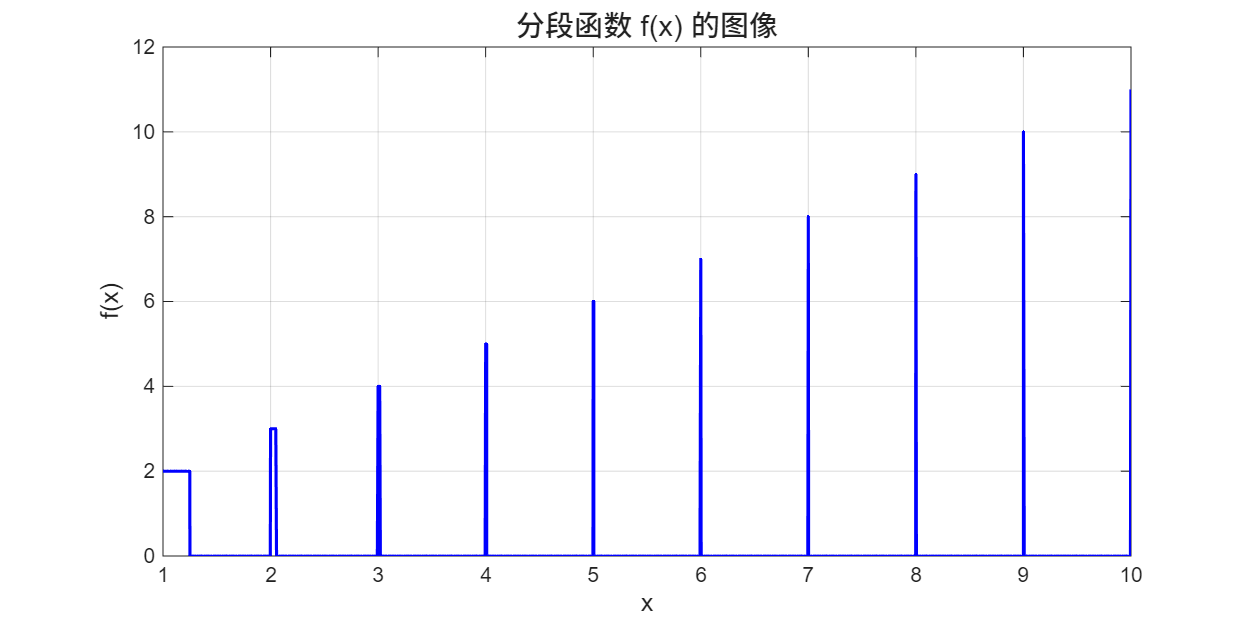
\includegraphics[width=0.7\linewidth]{figure/C7/untitled}
\end{center}

\begin{proof}
	对任意 $A>1$，取 $n \in \mathbb{N}$，使 $A \in [n,n+1)$.由 $f(x) \ge 0$，有
	\[
	\int_1^n f(x)\dd x \le \int_1^A f(x)\dd x \le \int_1^{n+1} f(x)\dd x
	\]
	
	当 $n \to +\infty$ 时，
	\[
	\begin{aligned}
		\lim_{n \to \infty} \int_1^n f(x)\dd x &= \lim_{n \to \infty} \left[ \int_1^2 f(x)\dd x + \dots + \int_{n-1}^n f(x)\dd x \right] \\
		&= \lim_{n \to \infty} \left[ \frac{1}{1 \cdot 2} + \frac{1}{2 \cdot 3} + \dots + \frac{1}{(n-1)n} \right] \\
		&= \lim_{n \to \infty} \left( 1 - \frac{1}{2} + \frac{1}{2} - \frac{1}{3} + \dots + \frac{1}{n-1} - \frac{1}{n} \right) \\
		&= \lim_{n \to \infty} \left( 1 - \frac{1}{n} \right) = 1
	\end{aligned}
	\]
	
	同理
	\[
	\lim_{n \to \infty} \int_1^{n+1} f(x)\dd x = 1
	\]
	由夹逼性
	\[
	\int_1^{+\infty} f(x)\dd x = 1
	\]
	
	
\end{proof} 
类似的方式，即使 $f(x)$ 在 $[a,+\infty)$ 连续（$n$ 次可微），也可以构造出使 $\displaystyle\int_a^{+\infty} f(x)dx$ 收敛而 $f(x)$ 在 $[a,+\infty)$ 无界的例子.

对反常积分的计算，我们可以形式上认为
\[
\int_a^{+\infty} f(x)\dd x = \lim_{A \to +\infty} F(A) - F(a)
\]

%
% 第7节：反常积分验敛法
% !TEX root = ../../../main.tex
% 所属：第一部分：单变量分析学 / 第8章：Riemann积分
% 节：8.7 反常积分验敛法
% 正文按原文件顺序保存；由 ../chapter8.tex 调用。
\section{反常积分验敛法}
\begin{proposition}（Cauchy 收敛原理）
	\[
	\int_a^{+\infty} f(x)\dd x \text{ 收敛} \iff
	\]
	$\forall \varepsilon>0$，$\exists M>0$ 且 $M \ge a$，使得 $\forall A_1,A_2 \ge M$，都有
	\[
	\left| \int_{A_2}^{A_1} f(x)\dd x \right| < \varepsilon
	\]
\end{proposition}
\begin{proof}
	由函数极限的 Cauchy 收敛原理易得.
\end{proof}
同时，我们给出无限区间上反常积分的 Cauchy 不收敛原理.

\begin{proposition}
	\[
	\int_a^{+\infty} f(x)\dd x \text{ 发散} \iff \exists \varepsilon_0>0,\ \forall M>0 \text{ 且 } M \ge a,\ \forall A_1,A_2 \ge M,
	\]
	都有
	\[
	\left| \int_{A_2}^{A_1} f(x)\dd x \right| \ge \varepsilon_0
	\]
	
\end{proposition}
\begin{definition}
	对 $f(x)$，若
	\[
	\int_a^{+\infty} |f(x)|\dd x
	\]
	收敛，则称 $\displaystyle\int_a^{+\infty} f(x)\dd x$ 绝对收敛，又称 $f(x)$ 在 $[a,+\infty)$ 绝对可积.
	
\end{definition}

\begin{proposition}
	若 $\displaystyle\int_a^{+\infty} f(x)\dd x$ 绝对收敛，则 $\displaystyle\int_a^{+\infty} f(x)\dd x$ 收敛.
\end{proposition}
\begin{proof}
	由 $\displaystyle\int_a^{+\infty} |f(x)|\dd x$ 收敛，$\forall \varepsilon>0$，$\exists M>0$ 且 $M \ge a$，使得 $\forall A_1,A_2 \ge M$ 且 $A_1>A_2$，有
	\[
	\int_{A_2}^{A_1} |f(x)|\dd x < \varepsilon
	\]
	而 $f \in \mathcal{R}[A_2,A_1]$，故
	\[
	\left| \int_{A_2}^{A_1} f(x)dx \right| \le \int_{A_2}^{A_1} |f(x)|\dd x < \varepsilon
	\]
	由Cauchy收敛原理，$\displaystyle\int_a^{+\infty} f(x)\dd x$ 收敛.
\end{proof}

\begin{definition}
	若 $\displaystyle\int_a^{+\infty} f(x)\dd x$ 收敛，但 $\displaystyle\int_a^{+\infty} |f(x)|\dd x$ 发散，则称 $\displaystyle\int_a^{+\infty} f(x)\dd x$ 条件收敛.
	
\end{definition}
下面我们考虑定号函数反常积分的敛散性
\begin{proposition}（比较验敛法）\label{比较验敛法}
	设函数 $f$ 在 $[a,+\infty)$ 上有定义，$\exists A \ge a$，使得 $f(x)$ 在 $[A,+\infty)$ 上满足 $f \ge 0$（或 $f \le 0$），函数 $\varphi$ 在 $[A,+\infty)$ 上满足
	\[
	0 \le f(x) \le k \varphi(x), \quad k \ge 0
	\]
	则
	\begin{enumerate}
		\item 若 $\displaystyle\int_a^{+\infty} \varphi(x)\dd x$ 收敛 $\implies \displaystyle\int_a^{+\infty} f(x)\dd x$ 收敛；
		\item 若 $\displaystyle\int_a^{+\infty} f(x)\dd x$ 发散 $\implies \displaystyle\int_a^{+\infty} \varphi(x)\dd x$ 发散.
	\end{enumerate}
	
	
\end{proposition}


\begin{proof}
	显然地，1 与 2 互为逆否命题，只需证明 1.
	
	由 $\displaystyle\int_a^{+\infty} \varphi(x)\dd x$ 收敛，根据 Cauchy 收敛准则，
	$\forall \varepsilon>0$，$\exists M \ge A$，$\forall A_1,A_2 \ge M$ 且 $A_1 \le A_2$，有
	\[
	0 < \int_{A_1}^{A_2} \varphi(x)\dd x < \varepsilon
	\]
	于是
	\[
	0 \le \int_{A_1}^{A_2} f(x)\dd x \le k \int_{A_1}^{A_2} \varphi(x)\dd x < k\varepsilon
	\]
	故 $\displaystyle\int_a^{+\infty} f(x)\dd x$ 收敛.
\end{proof} 
下面给出\ref{比较验敛法}的极限形式
\begin{corollary}
	设 $f(x)$ 与 $\varphi(x)$ 在 $[a,+\infty)$ 为非负函数，且
	\[
	\lim_{x \to +\infty} \frac{f(x)}{\varphi(x)} = l
	\]
	\begin{enumerate}
		\item 若 $0 \le l < +\infty$，则
		\[
		\int_a^{+\infty} \varphi(x)\dd x \text{ 收敛} \implies \int_a^{+\infty} f(x)\dd x \text{ 收敛}
		\] 
		\item  若 $0 < l \le +\infty$，则
		\[
		\int_a^{+\infty} \varphi(x)\dd x \text{ 发散} \implies \int_a^{+\infty} f(x)\dd x \text{ 发散}
		\]
	\end{enumerate}
	
	也就是说，$0<l<+\infty$时,$\varphi(x)$ 与 $f(x)$ 有相同的敛散性.
	
\end{corollary}
\begin{proof}
	\begin{enumerate}
		\item 由 $\lim\limits_{x \to +\infty} \dfrac{f(x)}{\varphi(x)} = l < +\infty$，则对 $\varepsilon=1$，$\exists M_0 \ge a$，当 $x > M_0$ 时
		\[
		0 \le \frac{f(x)}{\varphi(x)} - l < 1
		\]
		即
		\[
		0 \le l\varphi(x) \le f(x) \le (1+l)\varphi(x)
		\]
		由 $\displaystyle\int_a^{+\infty} \varphi(x)\dd x$ 收敛，推出 $\displaystyle\int_a^{+\infty} f(x)\dd x$ 收敛.
		
		\item 若 $0 < l \le +\infty$，令 $l' = \dfrac{1}{l}$，则 $0 \le l' < +\infty$，且
		\[
		\lim_{x \to +\infty} \frac{\varphi(x)}{f(x)} = l' \in [0,+\infty)
		\]
		对 $\varepsilon=1$，$\exists \widetilde{M}_0 \ge a$，$\forall x > \widetilde{M}_0$，有
		\[
		0 \le \frac{\varphi(x)}{f(x)} \le l' + 1
		\]
		即
		\[
		0 \le \varphi(x) \le (l'+1)f(x)
		\]
		由 $\displaystyle\int_a^{+\infty} \varphi(x)\dd x$ 发散，得 $\displaystyle\int_a^{+\infty} f(x)\dd x$ 发散.
	\end{enumerate}
\end{proof}
使用 $p$-积分与比较验敛法，我们得到 Cauchy 判别法.
\begin{corollary}
	（Cauchy 判别法）
	在 $[a,+\infty) \subset (0,+\infty)$ 上恒有 $f(x) \ge 0$，$K$ 是正常数.
	
	(1) 若 $f(x) \le \dfrac{K}{x^p}$，且 $p>1$，则 $\displaystyle\int_a^{+\infty} f(x)\dd x$ 收敛；
	
	(2) 若 $f(x) \ge \dfrac{K}{x^p}$，且 $p \le 1$，则 $\displaystyle\int_a^{+\infty} f(x)\dd x$ 发散.
\end{corollary}
\begin{corollary}
	（Cauchy 判别法的极限形式）
	设在 $[a,+\infty) \subset (0,+\infty)$ 上恒有 $f(x) \ge 0$，且
	\[
	\lim_{x \to +\infty} x^p f(x) = l
	\]
	则
	
	(1) 若 $0 \le l < +\infty$ 且 $p>1$，则 $\displaystyle\int_a^{+\infty} f(x)\dd x$ 收敛；
	
	(2) 若 $0 < l \le +\infty$ 且 $p \le 1$，则 $\displaystyle\int_a^{+\infty} f(x)\dd x$ 发散.
\end{corollary}


下面，我们先再次证明第二积分中值定理的一个特殊情况，证明的方法更有技巧性.
\begin{proposition}
	设 $f$ 在 $[a,b]$ 上连续且常义可积，$g$ 在 $[a,b]$ 上单调、连续可导且常义可积，则 $\exists \xi \in [a,b]$，使得
	\[
	\int_a^b f(x)g(x)\dd x = g(a)\int_a^\xi f(x)x + g(b)\int_\xi^b f(x)\dd x
	\]
\end{proposition}
\begin{proof}
	令 $F(x) = \displaystyle\int_a^x f(t)\dd t$，因 $f(x)$ 连续，故 $F'(x)=f(x)$.由分部积分法，
	\[
	\begin{aligned}
		\int_a^b f(x)g(x)\dd x &= \int_a^b g(x) d\left( \int_a^x f(t)\dd t \right) \\
		&= \left. g(x)F(x) \right|_a^b - \int_a^b F(x)g'(x)\dd x
	\end{aligned}
	\]
	因 $g$ 单调，故 $g'(x)$ 在 $[a,b]$ 上不变号，由积分第一中值定理，$\exists \xi \in [a,b]$，使得
	\[
	\int_a^b F(x)g'(x)dx = F(\xi)\int_a^b g'(x)\dd x
	\]
	代入上式得
	\[
	\begin{aligned}
		\int_a^b f(x)g(x)\dd x &= g(b)F(b) - F(\xi)\int_a^b g'(x)\dd x \\
		&= g(b)\int_a^b f(x)\dd x - \int_a^\xi f(x)\dd x \cdot \left( g(b)-g(a) \right) \\
		&= g(a)\int_a^\xi f(x)\dd x + g(b)\int_\xi^b f(x)\dd x
	\end{aligned}
	\]
\end{proof}

下面介绍 A-D 判别法.
\begin{proposition}(A-D 判别法)
	
	\begin{enumerate}
		\item Abel 判别法：若 $\displaystyle\int_a^{+\infty} f(x)\dd x$ 收敛，$g(x)$ 在 $[a,+\infty)$ 上单调有界，则 $\displaystyle\int_a^{+\infty} f(x)g(x)\dd x$ 收敛.
		\item Dirichlet 判别法：若 $F(A)=\displaystyle\int_a^A f(x)\dd x$ 在 $[a,+\infty)$ 上有界，$g(x)$ 在 $[a,+\infty)$ 上单调且 $\lim\limits_{x \to +\infty} g(x)=0$，则 $\displaystyle\int_a^{+\infty} f(x)g(x)\dd x$ 收敛.
	\end{enumerate}
\end{proposition}
\begin{proof}
	\begin{enumerate}
		\item 由 $g(x)$ 在 $[a,+\infty)$ 上有界，$\exists M \ge 0$，使得 $|g(x)| \le M$ 对 $\forall x \in [a,+\infty)$ 成立.
		因 $\displaystyle\int_a^{+\infty} f(x)\dd x$ 收敛，由 Cauchy 收敛准则，$\forall \varepsilon>0$，$\exists G \ge a$，对 $\forall A_1,A_2 > G$ 且 $A_1 < A_2$，有
		\[
		\left| \int_{A_1}^{A_2} f(x)\dd x \right| < \varepsilon
		\]
		由第二积分中值定理，$\exists \xi \in [A_1,A_2]$，使得
		\[
		\int_{A_1}^{A_2} f(x)g(x)dx = g(A_1)\int_{A_1}^\xi f(x)dx + g(A_2)\int_\xi^{A_2} f(x)dx
		\]
		因此
		\[
		\begin{aligned}
			\left| \int_{A_1}^{A_2} f(x)g(x)\dd x \right|
			&= \left| g(A_1)\int_{A_1}^\xi f(x)\dd x + g(A_2)\int_\xi^{A_2} f(x)\dd x \right| \\
			&\le |g(A_1)| \cdot \left| \int_{A_1}^\xi f(x)\dd x \right| + |g(A_2)| \cdot \left| \int_\xi^{A_2} f(x)\dd x \right| \\
			&\le M \left( \left| \int_{A_1}^\xi f(x)\dd x \right| + \left| \int_\xi^{A_2} f(x)\dd x \right| \right) \\
			&< 2M\varepsilon
		\end{aligned}
		\]
		由 Cauchy 收敛准则，$\displaystyle\int_a^{+\infty} f(x)g(x)\dd x$ 收敛.
		\item 由 $F(A)=\displaystyle\int_a^A f(x)\dd x$ 在 $[a,+\infty)$ 上有界，$\exists L>0$，对 $\forall A \in [a,+\infty)$，有
		\[
		|F(A)| = \left| \int_a^A f(x)\dd x \right| < L
		\]
		由 $\lim\limits_{x \to +\infty} g(x)=0$，$\forall \varepsilon>0$，$\exists X > a$，对 $\forall x > X$，有 $|g(x)| < \varepsilon$.
		对 $\forall A_1,A_2 > X$ 且 $A_1 \le A_2$，有 $|g(A_1)| < \varepsilon$，$|g(A_2)| < \varepsilon$.
		由第二积分中值定理，$\exists \xi \in [A_1,A_2]$，使得
		\[
		\int_{A_1}^{A_2} f(x)g(x)\dd x = g(A_1)\int_{A_1}^\xi f(x)\dd x + g(A_2)\int_\xi^{A_2} f(x)\dd x
		\]
		因此
		\[
		\begin{aligned}
			\left| \int_{A_1}^{A_2} f(x)g(x)\dd x \right|
			&= \left| g(A_1)\int_{A_1}^\xi f(x)\dd x + g(A_2)\int_\xi^{A_2} f(x)\dd x \right| \\
			&\le |g(A_1)| \cdot \left| \int_{A_1}^\xi f(x)\dd x \right| + |g(A_2)| \cdot \left| \int_\xi^{A_2} f(x)\dd x \right| \\
			&< \varepsilon \left( \left| \int_a^\xi f(x)\dd x - \int_a^{A_1} f(x)\dd x \right| + \left| \int_a^{A_2} f(x)\dd x - \int_a^\xi f(x)\dd x \right| \right) \\
			&< \varepsilon (L + L + L + L) = 4L\varepsilon
		\end{aligned}
		\]
		由 Cauchy 收敛准则，$\displaystyle\int_a^{+\infty} f(x)g(x)\dd x$ 收敛.
	\end{enumerate}
	
	
\end{proof}
\begin{example}
	考虑反常积分 $$ \int_0^{+\infty} \frac{\sin x}{x} \dd x$$ 的敛散性.
\end{example}
\begin{solution}
	将积分拆分为两部分：
	\[
	\int_0^{+\infty} \frac{\sin x}{x} dx = \int_0^1 \frac{\sin x}{x} dx + \int_1^{+\infty} \frac{\sin x}{x} dx = I + J
	\]
	
	对于 $I = \displaystyle\int_0^1 \dfrac{\sin x}{x} \dd x$：
	由于 $\lim\limits_{x\to0} \dfrac{\sin x}{x} = 1$，因此被积函数在 $x=0$ 附近有界，$I$ 是常义（Riemann）积分，必然收敛.
	
	对于 $J = \displaystyle\int_1^{+\infty} \dfrac{\sin x}{x} \dd x$：
	应用 Dirichlet 判别法：
	令 $f(x) = \sin x$，$g(x) = \dfrac{1}{x}$.
	
	1.  $F(A) = \displaystyle\int_1^A \sin x \dd x = -\cos A + \cos 1$ 在 $[1,+\infty)$ 上显然有界.
	
	2.  $g(x) = \dfrac{1}{x}$ 在 $[1,+\infty)$ 上单调递减，且 $\lim\limits_{x\to+\infty} g(x) = 0$.
	故 $J$ 收敛，因此原积分 $\displaystyle \int_0^{+\infty} \dfrac{\sin x}{x} \dd x$ 收敛.
	
	接下来判断其是否绝对收敛：
	\[
	\int_0^{+\infty} \left| \frac{\sin x}{x} \right| \dd x \ge \int_0^{+\infty} \frac{|\sin x|}{x} \dd x
	\]
	利用恒等式 $|\sin x|^2 = \sin^2 x = \dfrac{1-\cos 2x}{2}$，有：
	\[
	\int_0^{+\infty} \frac{|\sin x|}{x} \dd x \ge \int_0^{+\infty} \frac{\sin^2 x}{x} \dd x = \int_0^{+\infty} \frac{1-\cos 2x}{2x} \dd x = \int_0^{+\infty} \frac{1}{2x} \dd x - \int_0^{+\infty} \frac{\cos 2x}{2x} \dd x
	\]
	其中，$\displaystyle \int_0^{+\infty} \frac{1}{2x} dx$ 是 $p=1$ 的 $p$-积分，发散因此，原不等式右边整体发散，从而 $\displaystyle \int_0^{+\infty} \left| \frac{\sin x}{x} \right| dx$ 发散.
	
	综上，$\displaystyle \int_0^{+\infty} \frac{\sin x}{x} \dd x$ 条件收敛.
\end{solution}
对于有限闭区间上的无界函数的反常积分
\[
\int_a^b f(x)\dd x
\]
且 \(f(x)\) 在 \([a,b]\) 上有唯一的奇点 \(b\)。我们作变换
\[
t=\frac{1}{b-x},
\]
那么
\[
I=\int_a^b f(x)\dd x=\int_{\tfrac{1}{b-a}}^{+\infty} \frac{1}{t^2} f\left(b-\frac{1}{t}\right) \dd t.
\]
我们可以得到对应的 Cauchy 收敛原理、Cauchy 判别法与 A-D 判别法。
\begin{proposition}
	对上述的 $\displaystyle \int_a^b f(x)\dd x$ 收敛的充分必要条件是：
	$\forall \varepsilon>0,\ \exists \delta>0$，对任意 $\eta,\eta' \in (0,\delta)$，有
	\[
	\left| \int_{b-\eta}^{b-\eta'} f(x)\dd x \right| < \varepsilon
	\]
\end{proposition}
\begin{proposition}
	设在 $[a,b)$ 上恒有 $f(x) \ge 0$，若当 $x$ 属于 $b$ 的某个左邻域 $[b-\eta_0,b)$ 时，存在正常数 $K$与函数$\varphi(x)$，使得
	\begin{enumerate}
		\item 若 $f(x) \le K\varphi(x)$ 且 $\displaystyle\int_a^b \varphi(x)\dd x$收敛，则 $\displaystyle \int_a^b f(x)\dd x$ 收敛；
		\item 若 $f(x) \ge  K\varphi(x)$ 且$\displaystyle\int_a^b \varphi(x)\dd x$发散，则 $\displaystyle \int_a^b f(x)\dd x$ 发散。
	\end{enumerate}
\end{proposition}
\begin{proposition}
	设在 $[a,b)$ 上恒有 $f(x),\varphi(x) \ge 0$，且
	\[
	\lim_{x \to b^-} \dfrac{f(x)}{\varphi(x)} = l
	\]
	则
	\begin{enumerate}
		\item 若 $0 \le l < +\infty$ 且 $\displaystyle\int_a^b \varphi(x)\dd x$收敛，则 $\displaystyle \int_a^b f(x)\dd x$ 收敛；
		\item 若 $0 < l \le +\infty$ 且 $\displaystyle\int_a^b \varphi(x)\dd x$发散，则 $\displaystyle \int_a^b f(x)\dd x$ 发散。
	\end{enumerate}
	
\end{proposition}
\begin{proposition}
	设在 $[a,b)$ 上恒有 $f(x) \ge 0$，若当 $x$ 属于 $b$ 的某个左邻域 $[b-\eta_0,b)$ 时，存在正常数 $K$，使得\begin{enumerate}
		\item 若 $f(x) \le \dfrac{K}{(b-x)^p}$ 且 $p<1$，则 $\displaystyle \int_a^b f(x)\dd x$ 收敛；
		\item 若 $f(x) \ge \dfrac{K}{(b-x)^p}$ 且 $p \ge 1$，则 $\displaystyle \int_a^b f(x)\dd x$ 发散。
	\end{enumerate}
\end{proposition}
\begin{proposition}
	设在 $[a,b)$ 上恒有 $f(x) \ge 0$，且
	\[
	\lim_{x \to b^-} (b-x)^p f(x) = l
	\]
	则
	\begin{enumerate}
		\item 若 $0 \le l < +\infty$ 且 $p<1$，则 $\displaystyle \int_a^b f(x)\dd x$ 收敛；
		\item 若 $0 < l \le +\infty$ 且 $p \ge 1$，则 $\displaystyle \int_a^b f(x)\dd x$ 发散。
	\end{enumerate}
	
\end{proposition}
\begin{proposition}
	若下列两个条件之一满足，则 $\displaystyle \int_a^b f(x)g(x)\dd x$ 收敛：
	\begin{enumerate}
		\item \textbf{Abel 判别法}：$\displaystyle \int_a^b f(x)\dd x$ 收敛，$g(x)$ 在 $[a,b)$ 上单调有界；
		\item \textbf{Dirichlet 判别法}：$F(\eta)=\displaystyle \int_a^{b-\eta} f(x)\dd x$ 在 $(0,b-a]$ 上有界，$g(x)$ 在 $[a,b)$ 上单调且 $\lim_{x \to b^-} g(x)=0$。
	\end{enumerate}
\end{proposition}
\begin{proposition}
	设 $f(x)$ 在 $[a,+\infty)$ 上一致连续，且反常积分 $\displaystyle \int_a^{+\infty} f(x)\dd x$ 收敛，则
	\[
	\lim_{x\to+\infty} f(x)=0\]
\end{proposition}
\begin{proof}
	（反证法）
	若不然，即 $\lim\limits_{x\to+\infty} f(x)\neq 0$，则 $\exists \varepsilon_0>0$，对任意 $M>0$，总能找到 $x_0>M$，使得 $|f(x_0)|\ge \varepsilon_0$。
	
	取 $M_1=a+1$，则 $\exists x_1>M_1$，但 $|f(x_1)|\ge \varepsilon_0$；
	
	再取 $M_2=x_1+1$，则 $\exists x_2>M_2$，但$|f(x_2)|\ge \varepsilon_0$；
	
	$\vdots$
	
	以此类推，我们可以得到一个严格单调递增趋于 $+\infty$ 的数列 $\{x_n\}_{n=1}^\infty \subset [a,+\infty)$，满足 $|f(x_n)|\ge \varepsilon_0$。
	
	由于数列有无穷多个点，$f(x_n)$ 要么恒正，要么恒负。不失一般性，我们假设所有 $f(x_n)\ge \varepsilon_0>0$。
	
	由 $f(x)$ 在 $[a,+\infty)$ 上一致连续，对 $\dfrac{\varepsilon_0}{2}>0$，$\exists \delta_0>0$，使得对任意 $x',x''$，只要 $0<|x'-x''|<\delta_0$，就有
	\[
	|f(x')-f(x'')|<\frac{\varepsilon_0}{2}
	\]
	特别地，对任意 $x$ 满足 $|x-x_n|<\delta_0$，有
	\[
	f(x) > f(x_n) - \frac{\varepsilon_0}{2} \ge \varepsilon_0 - \frac{\varepsilon_0}{2} = \frac{\varepsilon_0}{2}
	\]
	因此，对任意 $n\ge 1$，有
	\[
	\int_{x_n-\delta_0/2}^{x_n+\delta_0/2} f(x)dx \ge \int_{x_n-\delta_0/2}^{x_n+\delta_0/2} \frac{\varepsilon_0}{2} dx = \delta_0 \cdot \frac{\varepsilon_0}{2} = C_0
	\]
	其中 $C_0=\dfrac{\delta_0\varepsilon_0}{2}>0$ 是一个常数。
	
	令 $y_n=x_n+\delta_0/2$，$y'_n=x_n-\delta_0/2$，则得到两个数列 $\{y_n\}$ 和 $\{y'_n\}$，它们都严格单调趋于 $+\infty$，且满足
	\[
	\int_{y'_n}^{y_n} f(x)dx \ge C_0
	\]
	这与反常积分 $\displaystyle \int_a^{+\infty} f(x)\dd x$ 收敛的 Cauchy 准则矛盾。
	
	因此，原命题成立，即 $\displaystyle \lim_{x\to+\infty} f(x)=0$。
	
	
\end{proof}
%
% 第8节：积分与级数
% !TEX root = ../../../main.tex
% 所属：第一部分：单变量分析学 / 第8章：Riemann积分
% 节：8.8 积分与级数
% 正文按原文件顺序保存；由 ../chapter8.tex 调用。
\section{积分与级数}
\begin{proposition}（积分判别法）
	设函数 $f(x)$ 在 $[a, +\infty)$ 上恒大于等于 $0$，取一个严格单调上升且趋于 $+\infty$ 的数列 $a_1 = a < a_2 < a_3 < \dots$，令
	\[
	u_n = \int_{a_n}^{a_{n+1}} f(x) \dd x
	\]
	则级数 $\sum u_n$ 与反常积分 $\displaystyle\int_{a}^{+\infty} f(x) \dd x$ 有相同的敛散性，并且当它们收敛时，
	\[
	\sum_{n=1}^{\infty} u_n = \int_{a}^{+\infty} f(x) \dd x
	\]
\end{proposition}



注意：当 $f(x) \ge 0$ 不成立时，由 $\displaystyle\int_{a}^{+\infty} f(x) \dd x$ 收敛可推得 $\sum u_n$ 收敛，但反之不成立。
例如：反常积分 $\displaystyle\int_{a}^{+\infty} \sin x \dd x$ 发散，但取 $u_n = \displaystyle\int_{n\pi}^{2n\pi} \sin x \dd x = 0$，此时级数 $\sum u_n$ 收敛。
\begin{proof}
	令 $F(A) = \displaystyle\int_{a}^{A} f(x) \dd x$。对任意 $A \ge a$，存在 $n$ 使得 $a_n \le A \le a_{n+1}$。设 $\sum u_n$ 的部分和为 $S_n$，则
	\begin{align*}
		\int_{a}^{A} f(x) \dd x
		&= \sum_{i=1}^{n-1} \int_{a_i}^{a_{i+1}} f(x) \dd x + \int_{a_n}^{A} f(x) \dd x \\
		&= S_{n-1} + \int_{a_n}^{A} f(x) \dd x
	\end{align*}
	由于 $f(x) \ge 0$，有
	\[
	S_{n-1} \le \int_{a}^{A} f(x) \dd x \le S_{n-1} + \int_{a_n}^{a_{n+1}} f(x) \dd x = S_n
	\]
	即
	\[
	S_{n-1} \le F(A) \le S_n
	\]
	\begin{itemize}
		\item 若 $\sum u_n$ 发散，则 $\{S_n\}$ 发散，从而 $F(A) \to +\infty$，即反常积分发散。
		\item 若 $\sum u_n$ 收敛，则 $\{S_n\}$ 收敛，从而 $F(A)$ 收敛，即反常积分收敛。
	\end{itemize}
	
	
	
\end{proof}
特别地，当 $f(x)$ 单调减少时，取 $a_n = n$，则当 $n \ge N = \lfloor a \rfloor + 1$ 时，有
\[
f(n+1) \le u_n = \int_{n}^{n+1} f(x) \dd x \le f(n)
\]
由比较判别法可知，级数 $\sum_{n=1}^{\infty} f(n)$ 与 $\sum_{n=1}^{\infty} u_n$ 同时收敛或发散，从而 $\sum_{n=1}^{\infty} f(n)$ 与反常积分 $\displaystyle\int_{a}^{+\infty} f(x) \dd x$ 同时收敛或发散。
\begin{example}
		考虑级数 $\sum_{n=2}^{\infty} \dfrac{1}{n(\ln n)^p}$ 的敛散性。
\end{example}


\begin{proof}
	与 \ref{级数1/nlnn}不同，我们用积分判别法来做。
	由积分判别法，级数 $\sum\limits_{n=2}^{\infty} \dfrac{1}{n(\ln n)^p}$ 与反常积分 $\displaystyle\int_{2}^{+\infty} \frac{1}{x(\ln x)^p} \mathrm{d}x$ 有相同的敛散性。
	
	故只需考虑反常积分 $\displaystyle\int_{2}^{+\infty} \frac{1}{x(\ln x)^p} \dd x$ 的敛散性。
	
	\[
	\int_{2}^{+\infty} \frac{1}{x(\ln x)^p} \dd x
	= \int_{2}^{+\infty} \frac{1}{(\ln x)^p} \dd (\ln x)
	=
	\begin{cases}
		\ln \ln x \Big|_{2}^{+\infty} \to +\infty, & p=1 \\[6pt]
		\dfrac{1}{1-p} (\ln x)^{1-p} \Big|_{2}^{+\infty}, & p \ne 1
	\end{cases}
	\]
	
	当 $1-p < 0$，即 $p>1$ 时，反常积分收敛；当 $p \le 1$ 时，反常积分发散。
	
	因此，级数 $\sum\limits_{n=2}^{\infty} \dfrac{1}{n(\ln n)^p}$ 当 $p>1$ 时收敛，当 $p \le 1$ 时发散。
	
\end{proof}
\begin{example}
	证明：
	
	1.  $\displaystyle \int_{0}^{+\infty} \frac{\dd x}{1+x^2\sin^2 x}$ 发散
	
	2.  $\displaystyle \int_{0}^{+\infty} \frac{\dd x}{1+x^4\sin^2 x}$ 收敛
\end{example}
\begin{solution}
	(1) 取 $a_n = n\pi,\ n=0,1,2,\dots$，令
	\[
	u_n = \int_{n\pi}^{(n+1)\pi} \frac{\dd x}{1+x^2\sin^2 x}
	= \int_{0}^{\pi} \frac{\dd t}{1+(n\pi+t)^2\sin^2 t}
	> \int_{0}^{\frac{1}{(n+1)\pi}} \frac{\dd t}{1+(n\pi+t)^2\sin^2 t}
	\]
	当 $0 < t < \dfrac{1}{(n+1)\pi}$ 时，有
	\[
	(n\pi+t)^2\sin^2 t < (n+1)^2\pi^2 t^2 < (n+1)^2\pi^2 \cdot \frac{1}{(n+1)^2\pi^2} = 1
	\]
	于是
	\[
	u_n > \int_{0}^{\frac{1}{(n+1)\pi}} \frac{\dd t}{1+1} = \frac{1}{2} \cdot \frac{1}{(n+1)\pi} = \frac{1}{2\pi} \cdot \frac{1}{n+1}
	\]
	因为级数 $\sum \dfrac{1}{n+1}$ 发散，由比较判别法可知 $\sum u_n$ 发散，故由积分判别法得 $\displaystyle \int_{0}^{+\infty} \frac{\dd x}{1+x^2\sin^2 x}$ 发散。
	
	(2) 取 $a_n = n\pi,\ n=0,1,2,\dots$，令
	\[
	u_n = \int_{n\pi}^{(n+1)\pi} \frac{\dd x}{1+x^4\sin^2 x}
	= \int_{0}^{\pi} \frac{\dd t}{1+(n\pi+t)^4\sin^2 t}
	\]
	将积分拆为两部分：
	\[
	u_n = \int_{0}^{\frac{\pi}{2}} \frac{\dd t}{1+(n\pi+t)^4\sin^2 t} + \int_{0}^{\frac{\pi}{2}} \frac{\dd t}{1+(n\pi+\pi-t)^4\sin^2 t} = u_n' + u_n''
	\]
	当 $0 < t < \dfrac{\pi}{2}$ 时，有 $\sin t \ge \dfrac{2}{\pi}t$，故
	\[
	(n\pi+t)^4\sin^2 t \ge n^4\pi^4 \left(\frac{2t}{\pi}\right)^2 = 4\pi^2n^4t^2
	\]
	于是
	\[
	u_n' \le \int_{0}^{\frac{\pi}{2}} \frac{\dd t}{1+4\pi^2n^4t^2}
	= \frac{1}{2\pi n^2} \int_{0}^{\pi^2n^2} \frac{\dd s}{1+s^2}
	< \frac{1}{2\pi n^2} \cdot \frac{\pi}{2} = \frac{1}{4n^2}
	\]
	由于级数 $\sum \dfrac{1}{n^2}$ 收敛，故 $\sum u_n'$ 收敛；同理可证 $\sum u_n''$ 收敛，因此 $\sum u_n$ 收敛，故由积分判别法得 $\displaystyle \int_{0}^{+\infty} \frac{\dd x}{1+x^4\sin^2 x}$ 收敛。
\end{solution}












































%

%% ===== 第一部分：单变量分析学 / 第9章：一些不定积分的问题 =====
% !TEX root = ../../main.tex
\setchapterimage{figure/chapter9封面图.png}
\setchapterintro{}
\chapter{一些不定积分的问题}
% 第1节：不定积分的修正
% !TEX root = ../../../main.tex
% 所属：第一部分：单变量分析学 / 第9章：一些不定积分的问题
% 节：9.1 不定积分的修正
% 正文按原文件顺序保存；由 ../chapter9.tex 调用。
\section{不定积分的修正}
\subsection*{常数修正}
也就是我们常常说的$+C$，与其他的教材不同的是，我们采取的是原函数的集合这一定义方式，所以常数修正在集合的意义下没有意义

这其实解释了很多初学者的疑惑，比如下面这个``悖论''：
\[
\int\frac{\dd x}{x}
=x\cdot \frac1x-\int x\cdot \dd\left(\frac1x\right)
=1+\int\frac{\dd x}{x},
\qquad\Longrightarrow\qquad 0=1.
\]
当然这并不是悖论，事实上\[0=1\equiv \{0+C:C\in \R\}=\{1+C:C\in\R\}\]

另外需要注意，只在结果后面装模作样地写上``$+C$（$C$ 是任意常数）''其实不一定能完成常数修正。这也是我们不再采用课本定义的原因。教材上的漏洞在修正体系下将被严肃对待.

\subsection*{``+C''的历史与实质}

在柯西（Cauchy）1823年的原始讲义中，不定积分的定义并非简单地``加一个任意常数''。柯西首先考虑了导数为零的函数：在连续情形下它可以被证明为常数，但在不连续情形下，它可能是\textbf{在每个连续区间上分别取不同常数值的函数}。因此，柯西定义的不定积分实际上是加了一个\textbf{函数}$\varphi(x)$，这个函数在每一个连续区间上恒为常数，但在不同区间上可以取不同的值。后续教材用字母 $C$ 代替 $\varphi(x)$ 作为简写，并强调``$C$ 不是一个固定不变的常数，也与 $x$ 的值无关''。

然而，这一精妙之处在代代相传中被简化成了``$+C$ 就是加任意常数''，丢掉了原定义最关键的细节。

\begin{figure}[H]
	\centering
	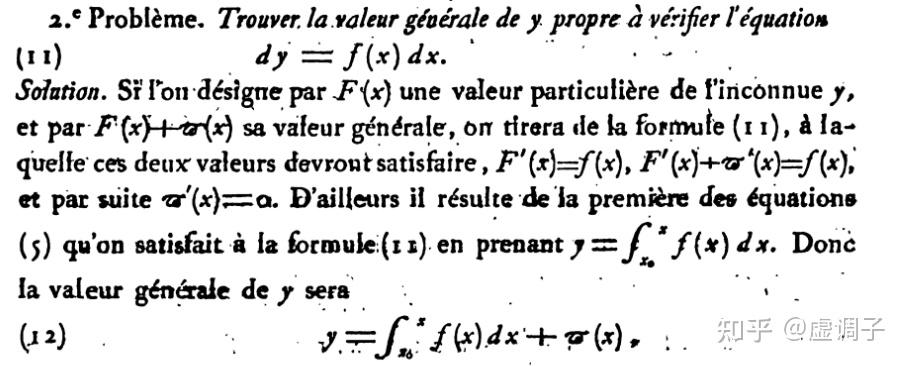
\includegraphics[width=0.85\linewidth]{figure/C9/005.jpg}
	\caption{柯西在1823年《无穷小分析讲义》中给出的不定积分定义：积分结果加上的是一个"函数"$\varphi(x)$，而非一个常数。}
\end{figure}

\begin{figure}[H]
	\centering
	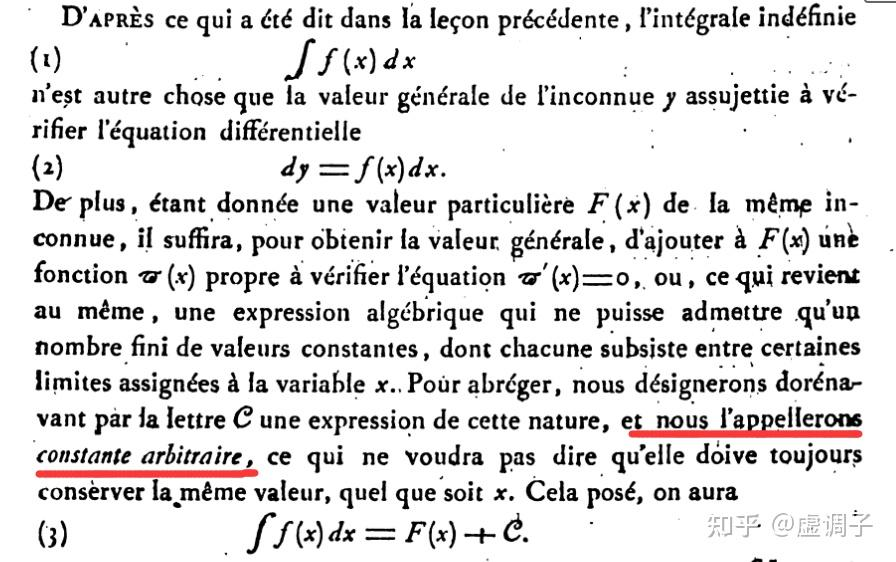
\includegraphics[width=0.85\linewidth]{figure/C9/007.jpg}
	\caption{柯西强调：用字母 $C$ 代替该函数只是简写，$C$ "不是一个固定不变的常数，也与 $x$ 的值无关"。}
\end{figure}

\begin{example}
	考虑 $\displaystyle\int\frac{\dd x}{x}$。常见答案 $\ln|x|+C$ 看似正确，实则不足。因为 $\frac1x$ 的定义域是 $(-\infty,0)\cup(0,+\infty)$，由两个不相连的区间组成。柯西定义下的真正结果是：

	\[
	\int\frac{\dd x}{x}=
	\begin{cases}
		\ln(-x)+C_1, & x<0,\\[4pt]
		\ln x+C_2,   & x>0,
	\end{cases}
	\]

	其中 $C_1$ 与 $C_2$ 是彼此独立的任意常数。仅写一个 $+C$ 会丢失一个自由度，因此在严格意义下是错误的。
\end{example}

\begin{figure}[H]
	\centering
	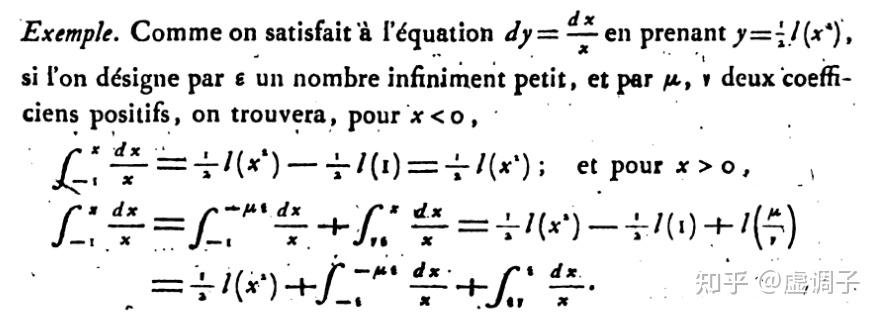
\includegraphics[width=0.85\linewidth]{figure/C9/009.jpg}
	\caption{柯西给出的 $\displaystyle\int\frac{\dd x}{x}=\frac12\ln(x^2)+\varpi(x)$，其中 $\varpi(x)$ 是各区间上独立的函数（现代记号写作 $\varphi(x)$ 或分段常数）。}
\end{figure}

\begin{example}
	更极端的情形出现在 $\displaystyle\int\frac{\dd x}{\cos^2x}$ 中。$\cos^2x$ 在 $x=\dfrac{\pi}{2}+k\pi$ 处为零，定义域被分割为无穷多个开区间：

	\[
	\int\frac{\dd x}{\cos^2x}=
	\begin{cases}
		\tan x+C_{-1}, & -\dfrac{3\pi}{2}<x<-\dfrac{\pi}{2},\\[6pt]
		\tan x+C_0,    & -\dfrac{\pi}{2}<x<\dfrac{\pi}{2},\\[6pt]
		\tan x+C_1,    & \dfrac{\pi}{2}<x<\dfrac{3\pi}{2},\\[6pt]
		\cdots
	\end{cases}
	\]

	此处需要\textbf{无穷多个}彼此独立的常数。这揭示了教科书公式表中 $\displaystyle\int\frac{\dd x}{\cos^2x}=\tan x+C$ 在严格意义下也是不完整的。
\end{example}

\subsection*{一个反例：传统$+C$导致的错误}

上述讨论并非咬文嚼字。在计算定积分时，若使用未经修正的不定积分公式，可能直接导致错误结果。

\begin{example}
	计算 $\displaystyle\int_0^{\pi}\frac{\dd x}{1+\sin^2x}$。

	采用传统公式
	\[
	\int\frac{\dd x}{1+\sin^2x}
	=\frac{1}{\sqrt2}\arctan\bigl(\sqrt2\tan x\bigr)+C,
	\]
	直接代入 Newton-Leibniz 公式：
	\[
	\int_0^{\pi}\frac{\dd x}{1+\sin^2x}
	=\left[\frac{1}{\sqrt2}\arctan\bigl(\sqrt2\tan x\bigr)+C\right]_0^{\pi}=0.
	\]

	但被积函数恒正，积分绝不可能为零。问题出在 $\tan x$ 在 $x=\dfrac{\pi}{2}$ 处间断，原函数在该点不连续，不能直接套用 Newton-Leibniz 公式。正确的做法是将积分区间在奇点处分段计算，或者使用经过\textbf{连续性修正}的结果（参见下文的连续修正方法），得到的真正结果是 $\dfrac{\pi}{\sqrt2}$。
\end{example}
\subsection*{$\operatorname{sgn}$ 与定义域修正}

由于开根号、去绝对值等操作会带来一个符号的差别，即原函数与所求得的表达式在定义域上相差一个符号，或者根据符号的需要缩小或扩大定义域，于是为了方便交流：
\begin{itemize}
	\item 后文将默认进行了对结果的 $\operatorname{sgn}$ 修正，变换过程省略。例如：
	\[
	\int \frac{\dd x}{x}=\ln(x)\bigl(=\ln|x|\bigr).
		\]
\end{itemize}


\begin{example}
	常用的
	\[
	\int \frac{\dd x}{1-x^2}=\operatorname{arth}x
	\]
	也可以认为默认进行了 $\operatorname{sgn}$ 修正。因为由 $\tanh x$ 的反函数来定义时，其定义域在 $|x|<1$。而不定积分的定义域要更广一些：
	\[
	\int\frac{\dd x}{1-x^2}=\operatorname{arth}x
	\left(=\frac12\ln\left|\frac{1+x}{1-x}\right|\right). 
	\]
	最直接的 $\operatorname{sgn}$ 修正就是利用 $\operatorname{sgn}()$ 函数解决。除此之外，取绝对值也是一种简单的 $\operatorname{sgn}$ 修正；对于复杂的函数将会有更复杂的修正结果。在追求结果的简洁和运算的简便方面，采用 $\operatorname{sgn}$ 修正是适合的。
	
	注意 $\operatorname{sgn}$ 修正不仅仅只有简单地添加符号，如
	\[
	\int\frac{\dd x}{1-x^2}
	=\frac12\operatorname{arth}\frac{2x}{1+x^2}. 
	\]
	相比 $\operatorname{arth}x$ 来说也是 $\operatorname{sgn}$ 修正，顺便将定义域扩大了。
\end{example}
\subsection*{连续性修正}
\begin{example}
	来尝试修正：
	\[
	\int\frac{\dd x}{1+\sin^2x}
	=\frac{1}{\sqrt2}\arctan\bigl(\sqrt2\tan x\bigr).
	\]
	原结果含有由 $\tan x$ 带来的间断。按照前面的思路，加上
	$x-\arctan(\tan x)$ 型的连续修正项，可得
	\[
	\begin{aligned}
		&\frac{1}{\sqrt2}\arctan\bigl(\sqrt2\tan x\bigr)
		-\frac{1}{\sqrt2}\arctan(\tan x)+\frac{x}{\sqrt2} \\
		&=\frac{1}{\sqrt2}\arctan
		\frac{(\sqrt2-1)\tan x}{1+\sqrt2\tan^2x}+\frac{x}{\sqrt2} \\
		&=\frac{1}{\sqrt2}\arctan
		\frac{(\sqrt2-1)\sin x\cos x}{\cos^2x+\sqrt2\sin^2x}+\frac{x}{\sqrt2} \\
		&=\frac{1}{\sqrt2}\arctan
		\frac{\sin 2x}{3+2\sqrt2-\cos 2x}+\frac{x}{\sqrt2}.
	\end{aligned}
	\]
	如图，由之前的间断函数变成了连续函数，连续修正成功。
\end{example}

\begin{figure}[H]
	\centering
	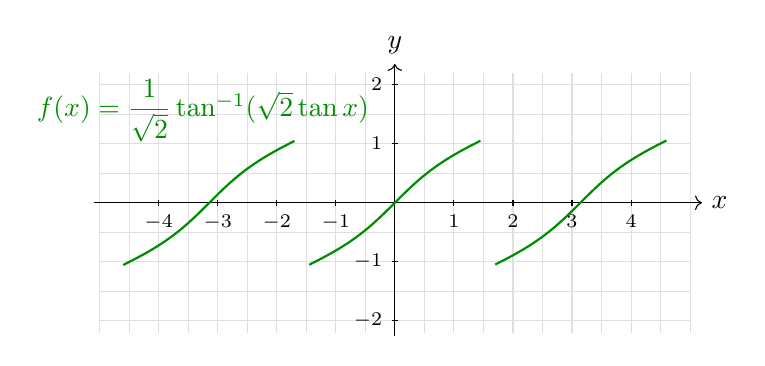
\begin{tikzpicture}[scale=0.75]
		\draw[gray!25, step=0.5] (-5,-2.2) grid (5,2.2);
		\draw[->] (-5.1,0)--(5.2,0) node[right] {$x$};
		\draw[->] (0,-2.25)--(0,2.35) node[above] {$y$};
		\foreach \x in {-4,-3,-2,-1,1,2,3,4}
		\draw (\x,0.05)--(\x,-0.05) node[below] {\scriptsize $\x$};
		\foreach \y in {-2,-1,1,2}
		\draw (0.05,\y)--(-0.05,\y) node[left] {\scriptsize $\y$};
		\draw[green!55!black, thick, domain=-4.6:-1.70, smooth, variable=\x]
		plot ({\x},{0.7071*rad(atan(1.4142*tan(\x r)))});
		\draw[green!55!black, thick, domain=-1.45:1.45, smooth, variable=\x]
		plot ({\x},{0.7071*rad(atan(1.4142*tan(\x r)))});
		\draw[green!55!black, thick, domain=1.70:4.6, smooth, variable=\x]
		plot ({\x},{0.7071*rad(atan(1.4142*tan(\x r)))});
		\node[green!55!black] at (-3.25,1.55)
		{$f(x)=\dfrac1{\sqrt2}\tan^{-1}(\sqrt2\tan x)$};
	\end{tikzpicture}
	\caption{不连续的结果}
\end{figure}

\begin{figure}[H]
	\centering
	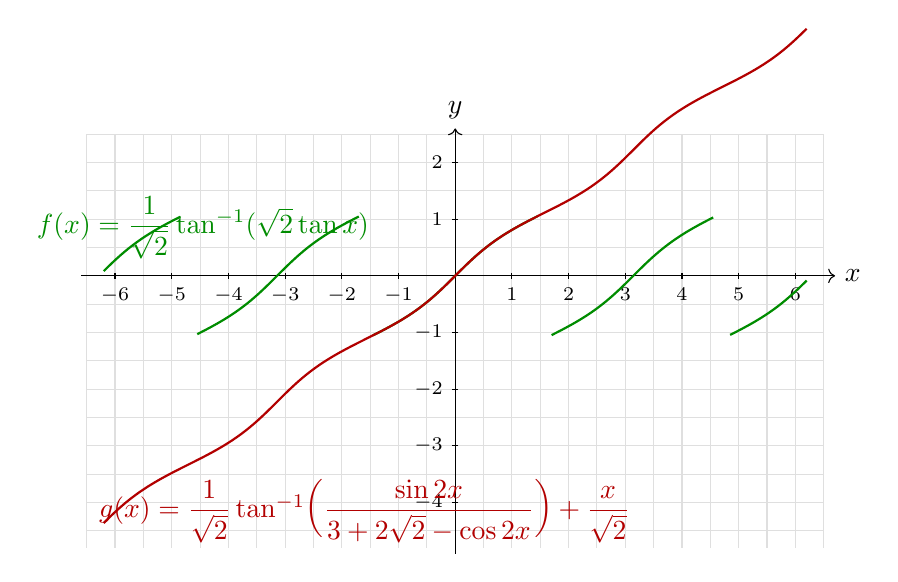
\begin{tikzpicture}[scale=0.72]
		\draw[gray!25, step=0.5] (-6.5,-4.8) grid (6.5,2.5);
		\draw[->] (-6.6,0)--(6.7,0) node[right] {$x$};
		\draw[->] (0,-4.9)--(0,2.6) node[above] {$y$};
		\foreach \x in {-6,-5,-4,-3,-2,-1,1,2,3,4,5,6}
		\draw (\x,0.05)--(\x,-0.05) node[below] {\scriptsize $\x$};
		\foreach \y in {-4,-3,-2,-1,1,2}
		\draw (0.05,\y)--(-0.05,\y) node[left] {\scriptsize $\y$};
		\draw[green!55!black, thick, domain=-6.2:-4.85, smooth, variable=\x]
		plot ({\x},{0.7071*rad(atan(1.4142*tan(\x r)))});
		\draw[green!55!black, thick, domain=-4.55:-1.70, smooth, variable=\x]
		plot ({\x},{0.7071*rad(atan(1.4142*tan(\x r)))});
		\draw[green!55!black, thick, domain=-1.45:1.45, smooth, variable=\x]
		plot ({\x},{0.7071*rad(atan(1.4142*tan(\x r)))});
		\draw[green!55!black, thick, domain=1.70:4.55, smooth, variable=\x]
		plot ({\x},{0.7071*rad(atan(1.4142*tan(\x r)))});
		\draw[green!55!black, thick, domain=4.85:6.2, smooth, variable=\x]
		plot ({\x},{0.7071*rad(atan(1.4142*tan(\x r)))});
		\draw[red!70!black, thick, domain=-6.2:6.2, samples=220, smooth, variable=\x]
		plot ({\x},{0.7071*rad(atan(sin(2*\x r)/(3+2*sqrt(2)-cos(2*\x r))))+\x/sqrt(2)});
		\node[green!55!black] at (-4.45,0.85)
		{$f(x)=\dfrac1{\sqrt2}\tan^{-1}(\sqrt2\tan x)$};
		\node[red!70!black] at (-1.6,-4.15)
		{$g(x)=\dfrac1{\sqrt2}\tan^{-1}\!\left(\dfrac{\sin2x}{3+2\sqrt2-\cos2x}\right)+\dfrac{x}{\sqrt2}$};
	\end{tikzpicture}
	\caption{修正后连续的结果}
\end{figure}

\subsection*{反正切修正}

通常，经过一些粗暴的换元后，定义域已四分五裂。我们如果想要实现相应的修正，就需要一些特定的计算方法了。下面讨论一些对反正切函数的修正。注意，修正的思路不是唯一的。

\begin{example}
	对 $f(x)=\arctan(k\tan x)$ 进行连续性修正。
	
	前面的例题其实也已经提到，思路是加上 $x-\arctan(\tan x)$，即
	\[
	\begin{aligned}
		\arctan(k\tan x)
		&=\arctan(k\tan x)+x-\arctan(\tan x) \\
		&=x+\arctan\frac{(k-1)\tan x}{1+k\tan^2x} \\
		&=x+\arctan\frac{(k-1)\sin(2x)}{(k+1)-(k-1)\cos(2x)}.
	\end{aligned}
	\]
\end{example}

\begin{example}
	对
	\[
	f(x)=\arctan\left(k\left(x-\frac1x\right)\right)
	\]
	的修正。
	
	思路来源于魏念辉（$k\neq0$），
	\[
	\begin{aligned}
		\arctan\left(k\left(x-\frac1x\right)\right)
		&=\arctan\left(k\left(x-\frac1x\right)\right)
		+\arctan\left(\frac1{kx}\right)+\arctan(kx) \\
		&=\arctan\left(kx^3+\left(\frac1k-1\right)x\right)+\arctan(kx).
	\end{aligned}
	\]
	这样是在 $\R$ 上连续的函数了。
	
	另外，值得一提的是对于一般的
	\[
	\arctan\frac{Q_n(x)}{P_n(x)}
	\]
	有机械的思路修正。
\end{example}

\begin{proposition}
	\textbf{反正切修正公式.}
	若 $f(x)=i$ 有 $n$ 个复解 $x_k=a_k+i b_k$，那么
	\[
	\arctan f(x)=\sum_{k=1}^{n}\arctan\frac{x-a_k}{b_k}. 
	\]
	等号是修正意义下的。
\end{proposition}

\begin{proof}
	留意到 $\ln$ 与 $\arctan$ 的一些关系，
	\[
	\begin{aligned}
		\arctan f(x)
		&=\operatorname{Im}\bigl[\ln(1+i\cdot f(x))\bigr] \\
		&=\operatorname{Im}\left[\ln\left(i\prod_{k=1}^{n}(x-x_k)\right)\right] \\
		&=\operatorname{Im}\sum_{k=1}^{n}\ln(x-a_k-i b_k) \\
		&=\sum_{k=1}^{n}\arctan\frac{x-a_k}{b_k}.
	\end{aligned}
	\]
	其中整体的常数相位被纳入修正意义之中。由此可以把所有简单的且各间断点的反正切结果修正。
\end{proof}

\begin{example}
	由反正切修正公式可以得到
	\[
	\arctan\left(\frac{x^3-x^2-4x-1}{x^3+4x^2+x-1}\right)
	=\arctan x+\arctan(x+1)+\arctan(1+2x).
	\]
\end{example}

除此之外，我们还可以注意到一种反正切的修正，这类甚至改变了函数名。我们考虑
\[
\int\frac{\dd x}{a+x^2}
=\frac1{\sqrt a}\arctan\frac{x}{\sqrt a}\quad(a>0). \tag{1.21}
\]
这里会自动限制 $a$ 的范围，来源于符号的局限性。如果考虑 $a<0$，由前章导数表中 $\operatorname{arth}$ 的导数公式可得
\[
\int\frac{\dd x}{a+x^2}
=-\frac1{\sqrt{-a}}\operatorname{arth}\frac{x}{\sqrt{-a}}\quad(a<0). 
\]
这两者在考虑复数域后是一致的，可以作为一种定义域修正处理。在后文中，如果 $a$ 的符号未知，那么我们采用 $\arctan$ 形式而省略定义域修正，以避免一些无聊的讨论。

如果考虑 $a=0$ 时，上式需要更进一步的修正，使得 $a$ 对于趋近极限过程连续。对于 $a>0$，也可以写成
\[
\int\frac{\dd x}{a+x^2}
=-\frac1{\sqrt a}\arctan\frac{\sqrt a}{x}\quad(a>0). 
\]
这样取极限都会有
\[
\int\frac{\dd x}{x^2}=-\frac1x. 
\]

\subsection*{取整函数的修正}

取整函数是指 $f(x)=[x]$，输出不超过 $x$ 的最大整数。由于分别在每个区域都是常数，所以取整函数的不定积分核心就是修正。

思路是采用多项式法。例如：
\[
\int [x]\dd x=x[x]+P_2([x])=x[x]-\frac12[x](1+[x]). 
\]
日常生活中，我们可能还会遇到小数部分函数，也即
\[
f(x)=\{x\}=x-[x]\geq0. 
\]
它们组合的更复杂的积分也可以利用多项式法修正，这里不详细展开，只举一个高次的例子：
\[
\int x\{x\}[x]\dd x
=\frac12x^2\{x\}^2-\frac23x\{x\}^3
+\frac16\{x\}^3+\frac13[x]^3+\frac16[x]^2. 
\]




%
% 第2节：一些用于计算不定积分的技巧
% !TEX root = ../../../main.tex
% 所属：第一部分：单变量分析学 / 第9章：一些不定积分的问题
% 节：9.2 一些用于计算不定积分的技巧
% 正文按原文件顺序保存；由 ../chapter9.tex 调用。
\section{一些用于计算不定积分的技巧}
%
% 第3节：简单的双元法
% !TEX root = ../../../main.tex
% 所属：第一部分：单变量分析学 / 第9章：一些不定积分的问题
% 节：9.3 简单的双元法
% 正文按原文件顺序保存；由 ../chapter9.tex 调用。
\section{简单的双元法}


%\section{Liouville定理}
%

%% ===== 第一部分：单变量分析学 / 第10章：一些定积分的问题 =====
% !TEX root = ../../main.tex
\setchapterimage{figure/chapter10封面图.png}
\setchapterintro{本章是 Riemann 积分理论的综合习题章，承接前两章对定积分基本理论的讨论，聚焦定积分在各个方向上的深入应用。全章共八节：第一节从积分定义出发，训练将和式转化为积分和以计算极限的技巧，沟通离散与连续；第二节围绕可积性展开，从振幅判别到连续点稠密性，层层揭示可积函数的精细结构；第三、四节讨论积分不等式的证明方法，包括辅助函数法、对称性与分部积分等；第五节整理积分中值定理的各类变体与应用；第六节介绍梯形公式、Simpson 公式等数值积分方法并结合编程实现；第七节处理面积、弧长、旋转体体积等几何应用；最后一节引入 Riemann--Stieltjes 积分，建立可积性理论并讨论其基本性质、}
\chapter{一些定积分的问题}
% 第1节：定积分定义与和式极限
% !TEX root = ../../../main.tex
% 所属：第一部分：单变量分析学 / 第10章：一些定积分的问题
% 节：10.1 定积分定义与和式极限
% 正文按原文件顺序保存；由 ../chapter10.tex 调用。
\section{定积分定义与和式极限}

本节主要讨论如何把有限和式写成定积分的积分和，从而计算极限。核心思想是：若 $f(x)$ 在 $[a,b]$ 上连续，且
\[
a=x_0<x_1<\cdots <x_n=b,\qquad \lambda_n=\max_{1\leq i\leq n}\Delta x_i\to 0,
\]
其中 $\Delta x_i=x_i-x_{i-1}$，$\xi_i\in[x_{i-1},x_i]$，则
\[
\lim_{n\to\infty}\sum_{i=1}^n f(\xi_i)\Delta x_i=\int_a^b f(x)\dd x.
\]



\begin{problem}
	求下列极限：
	\[
	\begin{aligned}
		&(1)\quad \lim_{n\to\infty}\left(\frac1{n^2+1}+\frac2{n^2+2}+\cdots+\frac n{n^2+n}\right),\\
		&(2)\quad \lim_{n\to\infty}\left(\frac1{n^2+1^2}+\frac2{n^2+2^2}+\cdots+\frac n{n^2+n^2}\right),\\
		&(3)\quad \lim_{n\to\infty}\left(\frac1{\sqrt{n^2+1^2}}+\frac1{\sqrt{n^2+2^2}}+\cdots+\frac1{\sqrt{n^2+n^2}}\right),\\
		&(4)\quad \lim_{n\to\infty}\left(\frac1{\sqrt{n^2+1}}+\frac1{\sqrt{n^2+2}}+\cdots+\frac1{\sqrt{n^2+n}}\right).
	\end{aligned}
	\]
\end{problem}

\begin{solution}
	(1) 有
	\[
	\frac{k}{n^2+k}=\frac1n\cdot \frac{\frac{k}{n}}{1+\frac{k}{n^2}},
	\]
	因为 $\dfrac1{1+k/n^2}\to1$ 且一致有界，故
	\[
	\sum_{k=1}^n\frac{k}{n^2+k}\to \int_0^1x\dd x=\frac12.
	\]
	
	(2) 有
	\[
	\frac{k}{n^2+k^2}=\frac1n\cdot\frac{\frac{k}{n}}{1+\left(\frac{k}{n}\right)^2},
	\]
	故
	\[
	\sum_{k=1}^n\frac{k}{n^2+k^2}\to
	\int_0^1\frac{x}{1+x^2}\dd x=\frac12\ln2.
	\]
	
	(3) 有
	\[
	\frac1{\sqrt{n^2+k^2}}=\frac1n\cdot\frac1{\sqrt{1+\left(\frac{k}{n}\right)^2}},
	\]
	故
	\[
	\sum_{k=1}^n\frac1{\sqrt{n^2+k^2}}\to
	\int_0^1\frac{\dd x}{\sqrt{1+x^2}}=\ln(1+\sqrt2).
	\]
	
	(4) 有
	\[
	\frac1{\sqrt{n^2+k}}=\frac1n\cdot\frac1{\sqrt{1+\frac{k}{n^2}}}.
	\]
	因为 $0\leq k/n^2\leq 1/n\to0$，所以
	\[
	\sum_{k=1}^n\frac1{\sqrt{n^2+k}}\to \int_0^1 1\dd x=1.
	\]
\end{solution}

\begin{problem}
	求极限
	\[
	\lim_{n\to\infty}\left(
	\frac{\sin\frac{\pi}{n}}{n+\frac1n}
	+\frac{\sin\frac{2\pi}{n}}{n+\frac2n}
	+\cdots+
	\frac{\sin\frac{n\pi}{n}}{n+\frac nn}
	\right).
	\]
\end{problem}

\begin{solution}
	一般项可写为
	\[
	\frac{\sin\frac{k\pi}{n}}{n+\frac{k}{n} }
	=\frac1n\cdot\frac{\sin\left(\pi\frac{k}{n}\right)}{1+\frac{k}{n^2}}.
	\]
	因为 $\dfrac{k}{n^2}\leq \dfrac1n\to0$，故原式是 $\sin(\pi x)$ 在 $[0,1]$ 上的积分和，因此
	\[
	\lim_{n\to\infty}\sum_{k=1}^n\frac{\sin\frac{k\pi}{n}}{n+\frac{k}{n} }
	=\int_0^1\sin(\pi x)\dd x=\frac2\pi.
	\]
\end{solution}

\begin{problem}
	取对数再用定积分定义，求下列极限：
	\[
	(1)\quad \lim_{n\to\infty}\frac{\sqrt[n]{n!}}{n};
	\qquad
	(2)\quad \lim_{n\to\infty}\frac{\sqrt[n]{(n+1)(n+2)\cdots(n+n)}}{n}.
	\]
\end{problem}

\begin{solution}
	(1) 设
	\[
	L_n=\frac{\sqrt[n]{n!}}{n}.
	\]
	取对数得
	\[
	\begin{aligned}
		\ln L_n
		&=\frac1n\ln(n!)-\ln n
		=\frac1n\sum_{k=1}^n\ln k-\ln n\\
		&=\frac1n\sum_{k=1}^n\ln\frac{k}{n}
		\to \int_0^1\ln x\dd x=-1.
	\end{aligned}
	\]
	因此
	\[
	\lim_{n\to\infty}\frac{\sqrt[n]{n!}}{n}=e^{-1}=\frac1e.
	\]
	
	(2) 设
	\[
	M_n=\frac{\sqrt[n]{(n+1)(n+2)\cdots(n+n)}}{n}.
	\]
	取对数得
	\[
	\begin{aligned}
		\ln M_n
		&=\frac1n\sum_{k=1}^n\ln(n+k)-\ln n\\
		&=\frac1n\sum_{k=1}^n\ln\left(1+\frac{k}{n}\right)
		\to \int_0^1\ln(1+x)\dd x=2\ln2-1.
	\end{aligned}
	\]
	所以
	\[
	\lim_{n\to\infty}M_n=e^{2\ln2-1}=\frac4e.
	\]
\end{solution}



\begin{problem}
	求极限
	\[
	\lim_{n\to\infty}\left(
	\frac{\sin\frac{\pi}{n}}{n+2026}
	+\frac{\sin\frac{2\pi}{n}}{n+\frac{2026}{2}}
	+\cdots+
	\frac{\sin\frac{n\pi}{n}}{n+\frac{2026}{n}}
	\right).
	\]
\end{problem}

\begin{solution}
	一般项为
	\[
	\frac{\sin\frac{k\pi}{n}}{n+\frac{2026}{k}}
	=\frac1n\cdot \frac{\sin\left(\pi\frac{k}{n}\right)}{1+\frac{2026}{kn}}.
	\]
	对任意固定的 $\delta\in(0,1)$，当 $k\geq \delta n$ 时，
	\[
	0\leq \frac{2026}{kn}\leq \frac{2026}{\delta n^2}\to0,
	\]
	因而这一段和趋于
	\[
	\int_\delta^1\sin(\pi x)\dd x.
	\]
	对 $1\leq k<\delta n$ 的前段，利用 $0\leq \sin(\pi k/n)\leq 1$，有
	\[
	0\leq \sum_{1\leq k<\delta n}\frac{\sin\frac{k\pi}{n}}{n+\frac{2026}{k}}
	\leq \frac{\lfloor \delta n\rfloor}{n}\leq \delta.
	\]
	令 $n\to\infty$ 后再令 $\delta\to0^+$，得原极限为
	\[
	\int_0^1\sin(\pi x)\dd x=\frac2\pi.
	\]
\end{solution}

\begin{problem}
	设 $\alpha>-1,\ \beta>-1$，求极限
	\[
	\lim_{n\to\infty}
	\frac{\left(1^\alpha+3^\alpha+\cdots+(2n+1)^\alpha\right)^{\beta+1}}
	{\left(2^\beta+4^\beta+\cdots+(2n)^\beta\right)^{\alpha+1}}.
	\]
\end{problem}

\begin{solution}
	将分子、分母分别化为 $[0,2]$ 上的积分和。因为
	\[
	\begin{aligned}
		1^\alpha+3^\alpha+\cdots+(2n+1)^\alpha
		&=n^\alpha\left[\left(\frac1n\right)^\alpha+
		\left(\frac3n\right)^\alpha+\cdots+
		\left(\frac{2n+1}{n}\right)^\alpha\right],\\
		2^\beta+4^\beta+\cdots+(2n)^\beta
		&=n^\beta\left[\left(\frac2n\right)^\beta+
		\left(\frac4n\right)^\beta+\cdots+
		\left(\frac{2n}{n}\right)^\beta\right].
	\end{aligned}
	\]
	于是
	\[
	\begin{aligned}
		&\frac{\left(1^\alpha+3^\alpha+\cdots+(2n+1)^\alpha\right)^{\beta+1}}
		{\left(2^\beta+4^\beta+\cdots+(2n)^\beta\right)^{\alpha+1}}\\
		&=2^{\alpha-\beta}
		\frac{\left[\dfrac2n\left(\left(\dfrac1n\right)^\alpha+
			\left(\dfrac3n\right)^\alpha+\cdots+
			\left(\dfrac{2n+1}{n}\right)^\alpha\right)\right]^{\beta+1}}
		{\left[\dfrac2n\left(\left(\dfrac2n\right)^\beta+
			\left(\dfrac4n\right)^\beta+\cdots+
			\left(\dfrac{2n}{n}\right)^\beta\right)\right]^{\alpha+1}}.
	\end{aligned}
	\]
	当 $n\to\infty$ 时，两个括号分别是 $f(t)=t^\alpha$ 与 $g(t)=t^\beta$ 在 $[0,2]$ 上的积分和。故
	\[
	\dfrac2n\sum_{i=1}^{n+1}\left(\frac{2i-1}{n}\right)^\alpha
	\to \int_0^2t^\alpha\dd t=\frac{2^{\alpha+1}}{\alpha+1},
	\]
	以及
	\[
	\dfrac2n\sum_{i=1}^{n}\left(\frac{2i}{n}\right)^\beta
	\to \int_0^2t^\beta\dd t=\frac{2^{\beta+1}}{\beta+1}.
	\]
	因此
	\[
	\begin{aligned}
		\lim_{n\to\infty}
		\frac{\left(1^\alpha+3^\alpha+\cdots+(2n+1)^\alpha\right)^{\beta+1}}
		{\left(2^\beta+4^\beta+\cdots+(2n)^\beta\right)^{\alpha+1}}
		&=2^{\alpha-\beta}
		\frac{\left(\dfrac{2^{\alpha+1}}{\alpha+1}\right)^{\beta+1}}
		{\left(\dfrac{2^{\beta+1}}{\beta+1}\right)^{\alpha+1}}\\
		&=2^{\alpha-\beta}\frac{(\beta+1)^{\alpha+1}}{(\alpha+1)^{\beta+1}}.
	\end{aligned}
	\]
\end{solution}
\begin{problem}
	求极限
	\[
	\lim_{n\to\infty}\left(b^{\frac1n}-1\right)
	\sum_{i=0}^{n-1}b^{\frac{i}{n}}\sin b^{\frac{2i+1}{2n}},\qquad b>1.
	\]
\end{problem}

\begin{solution}
	先把和式改写为
	\[
	\begin{aligned}
		&\left(b^{\frac1n}-1\right)
		\sum_{i=0}^{n-1}b^{\frac{i}{n}}\sin b^{\frac{2i+1}{2n}}  \\
		&=\sum_{i=0}^{n-1}\sin b^{\frac{2i+1}{2n}}
		\left(b^{\frac{i+1}{n}}-b^{\frac{i}{n}}\right).
	\end{aligned}
	\]
	令
	\[
	x_i=b^{\frac{i}{n}},\qquad i=0,1,\ldots,n.
	\]
	则
	\[
	1=x_0<x_1<\cdots <x_n=b,
	\qquad \Delta x_i=x_{i+1}-x_i=b^{\frac{i+1}{n}}-b^{\frac{i}{n}}.
	\]
	又
	\[
	\xi_i=b^{\frac{2i+1}{2n}}=\sqrt{b^{\frac{i}{n}}b^{\frac{i+1}{n}}}\in[x_i,x_{i+1}],
	\]
	且最大分割长度满足
	\[
	\lambda_n=\max_{0\leq i\leq n-1}\Delta x_i
	=b-b^{\frac{n-1}{n}}=b\left(1-b^{-\frac1n}\right)\to 0.
	\]
	因此原式是函数 $\sin x$ 在 $[1,b]$ 上的一个积分和，故
	\[
	\lim_{n\to\infty}\left(b^{\frac1n}-1\right)
	\sum_{i=0}^{n-1}b^{\frac{i}{n}}\sin b^{\frac{2i+1}{2n} }
	=\int_1^b\sin x\dd x=\cos 1-\cos b.
	\]
\end{solution}

\begin{problem}
	设 $f(x)$ 在 $[0,1]$ 上连续，证明
	\[
	\lim_{n\to\infty}\frac1n\sum_{k=1}^n(-1)^{k+1}f\left(\frac{k}{n}\right)=0.
	\]
\end{problem}

\begin{proof}
	记
	\[
	a_n=\frac1n\sum_{k=1}^n(-1)^{k+1}f\left(\frac{k}{n}\right).
	\]
	当 $n=2m$ 时，利用
	\[
	b_1-b_2+b_3-b_4+\cdots+b_{2m-1}-b_{2m}
	=(b_1+b_2+\cdots+b_{2m})-2(b_2+b_4+\cdots+b_{2m}),
	\]
	得
	\[
	\begin{aligned}
		a_{2m}
		&=\frac1{2m}\sum_{k=1}^{2m}f\left(\frac{k}{2m}\right)
		-\frac{2}{2m}\sum_{k=1}^{m}f\left(\frac{2k}{2m}\right)\\
		&=\frac1n\sum_{k=1}^{n}f\left(\frac{k}{n}\right)
		-\frac2n\sum_{k=1}^{m}f\left(\frac{2k}{n}\right).
	\end{aligned}
	\]
	第一项是 $f$ 在 $[0,1]$ 上右端点取样的积分和，所以
	\[
	\frac1n\sum_{k=1}^{n}f\left(\frac{k}{n}\right)\to \int_0^1 f(x)\dd x.
	\]
	第二项可看作把 $[0,1]$ 分成 $m$ 个小区间，每个小区间长度为 $1/m=2/n$，并取右端点 $2k/n$ 的积分和，所以
	\[
	\frac2n\sum_{k=1}^{m}f\left(\frac{2k}{n}\right)\to \int_0^1 f(x)\dd x.
	\]
	因此 $a_{2m}\to 0$。
	
	当 $n=2m+1$ 时，同理有
	\[
	\begin{aligned}
		a_{2m+1}
		&=\frac1n\sum_{k=1}^{n}f\left(\frac{k}{n}\right)
		-\frac2n\sum_{k=1}^{m}f\left(\frac{2k}{n}\right).
	\end{aligned}
	\]
	第二项对应的是 $[0,2m/n]$ 上的积分和，而 $2m/n\to 1$，故它仍趋于 $\int_0^1f(x)\dd x$；第一项也趋于同一积分。因此 $a_{2m+1}\to0$。
	
	综上，偶子列与奇子列极限都为 $0$，故
	\[
	\lim_{n\to\infty}a_n=0.
	\]
\end{proof}

%
% 第2节：可积性相关
% !TEX root = ../../../main.tex
% 所属：第一部分：单变量分析学 / 第10章：一些定积分的问题
% 节：10.2 可积性相关
% 正文按原文件顺序保存；由 ../chapter10.tex 调用。
\section{可积性相关}
\begin{proposition}
	若 $f(x)$ 在 $[a,b]$ 上的不连续点可以用有限个总长度任意小的区间覆盖，则 $f(x)$ 在 $[a,b]$ 上可积。
\end{proposition}

\begin{solution}
	设 $|f(x)|\leq M$。任取 $\varepsilon>0$。由题设，$f$ 的不连续点集 $D$ 可由有限个开区间 $I_1,\ldots,I_m$ 覆盖，且
	\[
	\sum_{k=1}^m |I_k|<\frac{\varepsilon}{4M}.
	\]
	记
	\[
	G=[a,b]\setminus\bigcup_{k=1}^m I_k.
	\]
	在 $G$ 上，$f$ 的每一点都是连续点。取分划$P$包含$a,b$与$\{I_m\}$所以的端点。由于 $G$ 是有限个闭区间的并，$f$ 在 $G$ 上一致连续。因此
	\[
	\omega_i(f)<\frac{\varepsilon}{2(b-a)},
	\]
	其中 $\omega_i(f)$ 为 $f$ 在G的小区间上的振幅。
	\[
	\sum_i\omega_i(f)\Delta x_i
	\leq \frac{\varepsilon}{2(b-a)}(b-a)+2M\sum_{k=1}^m |I_k|<\varepsilon.
	\]
	由可积的第二充要条件，$f\in \mathcal{R}[a,b]$。
\end{solution}


\begin{example}
	试说明下列函数在 $[0,1]$ 上可积：
	\[
	(1)\quad f(x)=\operatorname{sgn}\left(\sin\frac{\pi}{x}\right);
	\]
	\[
	(2)\quad
	f(x)=
	\begin{cases}
		\displaystyle \frac1x-\left[\frac1x\right],&x\ne0,\\[6pt]
		0,&x=0.
	\end{cases}
	\]
\end{example}


\begin{solution}
	两个函数的共同特点是：在 $[0,1]$ 上除点列
	\[
	\left\{\frac1n:n=1,2,\ldots\right\}
	\]
	以及聚点 $0$ 外，函数均连续。因此只需说明这些间断点可以由有限多个任意小的区间覆盖
	
	事实上，给定 $\varepsilon>0$，取 $N$ 充分大，使得
	\[
	\frac1N<\frac{\varepsilon}{4}.
	\]
	于是区间 $\left(-\dfrac{\varepsilon}{4},\dfrac{\varepsilon}{4}\right)$ 覆盖了聚点 $0$ 以及点列中除有限项外的所有点。剩下的有限个间断点
	\[
	1,\frac12,\ldots,\frac1N
	\]
	分别用长度小于 $\dfrac{\varepsilon}{2N}$ 的小区间覆盖。这样全部间断点可由有限个区间覆盖，且总长度小于
	\[
	\frac{\varepsilon}{2}+N\cdot\frac{\varepsilon}{2N}=\varepsilon.
	\]
	由于上述两个函数均有界，并且在这些区间外连续，故由上命题可知二者均在 $[0,1]$ 上可积。
\end{solution}
\begin{example}
	设 $f$ 是 $[a,b]$ 上的有界函数，且 $f$ 的不连续点全体包含于一个收敛点列
	\[
	x_1,x_2,\ldots,
	\qquad \lim_{n\to\infty}x_n=x\in[a,b].
	\]
	证明：$f\in R[a,b]$。
\end{example}


\begin{solution}
	记 $M>0$ 使得 $|f(t)|\leq M$。任取 $\varepsilon>0$。由于 $x_n\to x$，存在 $N$，使得当 $n>N$ 时，
	\[
	|x_n-x|<\delta_0,
	\]
	其中 $\delta_0>0$ 可取到足够小，使得包含 $x$ 及所有尾项 $x_{N+1},x_{N+2},\ldots$ 的小区间总长度小于 $\varepsilon/(4M)$。
	
	对有限个点 $x_1,\ldots,x_N$，分别取互不相交的小区间覆盖，使其长度总和小于 $\varepsilon/(4M)$。于是全部不连续点可由有限个区间覆盖，且这些区间长度总和小于 $\varepsilon/(2M)$。
	
	故由上命题可知二者均在 $[a,b]$ 上可积。
\end{solution}

\begin{problem}
	设 $f,g\in \mathcal{R}[a,b]$。证明
	\[
	\max\{f,g\},\qquad \min\{f,g\}
	\]
	也属于 $\mathcal{R}[a,b]$。
\end{problem}

\begin{solution}
	利用恒等式
	\[
	\max\{f,g\}=\frac12\bigl(f+g+|f-g|\bigr),
	\]
	\[
	\min\{f,g\}=\frac12\bigl(f+g-|f-g|\bigr),
	\]
	与线性性和绝对可积性 ，可知 $\max\{f,g\},\min\{f,g\}\in  \mathcal{R}[a,b]$。
\end{solution}

\begin{problem}
	设 $f(x)$ 在 $[0,a]$ 上二次可导，且
	\[
	f(0)=f'(0)=f'(a)=0,
	\qquad
	f(a)=1,
	\qquad
	|f''(x)|\leq1\quad (x\in[0,a]).
	\]
	令
	\[
	g(x)=
	\begin{cases}
		x,&0\leq x\leq \dfrac a2,\\[4pt]
		a-x,&\dfrac a2<x\leq a.
	\end{cases}
	\]
	证明：
	\[
	(1)\quad f'(x)\leq g(x)\quad (x\in[0,a]);
	\]
	\[
	(2)\quad \exists x_0\in[0,a],\quad f'(x_0)<g(x_0);
	\]
	\[
	(3)\quad a>2.
	\]
\end{problem}

\begin{solution}
	(1) 当 $x\in[0,a/2]$ 时，由 Lagrange 中值定理，存在 $\xi\in(0,x)$，使得
	\[
	f'(x)=f'(x)-f'(0)=f''(\xi)x\leq x=g(x).
	\]
	当 $x\in[a/2,a]$ 时，存在 $\eta\in(x,a)$，使得
	\[
	f'(x)=f'(x)-f'(a)=-f''(\eta)(a-x)\leq |f''(\eta)|(a-x)\leq a-x=g(x).
	\]
	故对所有 $x\in[0,a]$，均有 $f'(x)\leq g(x)$。
	
	(2) 若结论不成立，则对每个 $x\in[0,a]$ 都有
	\[
	f'(x)=g(x).
	\]
	则 $f'$ 在 $a/2$ 处不可导，这与 $f$ 二次可导矛盾。
	
	(3) \[
	1=f(a)-f(0)=\int_0^a f'(x)\dd x
	<\int_0^a g(x)\dd x=\int_0^{a/2}x\dd x+\int_{a/2}^a(a-x)\dd x
	=\frac{a^2}{4}.
	\]
	故
	\[
	1<\frac{a^2}{4},
	\]
	因为 $a>0$，所以 $a>2$。
\end{solution}

\begin{proposition}
		若 $f(x)$ 在 $[a,b]$ 上可积，则 $f(x)$ 的连续点在 $[a,b]$ 上处处稠密。
\end{proposition}
这是一个重要的命题，他告诉我们可积性对连续性最低的需求
\begin{solution}
	问题归结为证明：对任意闭区间 $[\alpha,\beta]\subset[a,b]$，$f$ 在 $[\alpha,\beta]$ 内至少有一个连续点。
	
	由于 $f\in  \mathcal{R}[a,b]$，故 $f\in R[\alpha,\beta]$。对 $\varepsilon_1=1/2$，存在 $[\alpha,
	\beta]$ 的一个分割 $T_1$，使得
	\[
	\sum \omega_i\Delta x_i<\frac12(\beta-\alpha).
	\]
	因此至少存在一个小区间，其上 $f$ 的振幅小于 $1/2$。否则所有小区间振幅均不小于 $1/2$，便有
	\[
	\sum \omega_i\Delta x_i\geq \frac12(\beta-\alpha),
	\]
	矛盾。适当缩小此小区间，得到闭区间 $[a_1,b_1]\subset(\alpha,\beta)$，并且
	\[
	b_1-a_1<\frac12(\beta-\alpha),
	\qquad
	\omega_f([a_1,b_1])<\frac12.
	\]
	
	以 $[a_1,b_1]$ 代替 $[\alpha,\beta]$，类似地可取
	\[
	[a_2,b_2]\subset(a_1,b_1),
	\qquad
	b_2-a_2<\frac12(b_1-a_1),
	\qquad
	\omega_f([a_2,b_2])<\frac1{2^2}.
	\]
	如此继续，得到闭区间套
	\[
	[a_1,b_1]\supset[a_2,b_2]\supset\cdots\supset[a_n,b_n]\supset\cdots,
	\]
	且
	\[
	0<b_n-a_n<\frac1{2^n}(\beta-\alpha)\to0,
	\qquad
	\omega_f([a_n,b_n])<\frac1{2^n}.
	\]
	由闭区间套定理，存在唯一点 $\xi$ 属于所有 $[a_n,b_n]$。因为 $a_n<\xi<b_n$，任取 $\varepsilon>0$，取 $n$ 使得 $2^{-n}<\varepsilon$，并令
	\[
	\delta=\min\{\xi-a_n,b_n-\xi\}>0.
	\]
	当 $|x-\xi|<\delta$ 时，$x\in[a_n,b_n]$，从而
	\[
	|f(x)-f(\xi)|\leq \omega_f([a_n,b_n])<\varepsilon.
	\]
	故 $f$ 在 $\xi$ 处连续。于是 $f$ 的连续点在 $[a,b]$ 上处处稠密。
\end{solution}
\begin{example}\label{连续点位令}
	证明：若 $f(x)\geq0$ 在 $[a,b]$ 上有定义并且可积，则等式
	\[
	\int_a^b f(x)\dd x=0
	\]
	成立的充要条件是：$f(x)$ 在连续点上恒为零。
\end{example}
\begin{solution}
	必要性：若存在连续点 $x_0\in[a,b]$，使得 $f(x_0)>0$，则可取 $\delta>0$，使得在 $[a,b]\cap(x_0-\delta,x_0+\delta)$ 内有
	\[
	f(x)>\frac12 f(x_0)>0.
	\]
	于是
	\[
	\int_a^b f(x)\dd x\geq
	\int_{[a,b]\cap(x_0-\delta,x_0+\delta)} f(x)\dd x>0,
	\]
	与积分为零矛盾。因此 $f$ 在连续点上必为零。
	
	充分性：设 $f$ 在其所有连续点上均为零。由于 $f\in  \mathcal{R}[a,b]$，由上命题 可知其连续点在任意小区间中都存在。取$\xi_i$为相应小区间上的连续点
	\[\int_a^b f(x) = \sum f(\xi_i)\Delta_i = 0\]
\end{solution}
\begin{example}
	设 $f(x)$ 在 $[a,b]$ 上可积。证明：对于 $[a,b]$ 上任一可积函数 $g(x)$，恒有
	\[
	\int_a^b f(x)g(x)\dd x=0,
	\]
	则函数 $f(x)$ 在连续点上恒为零。
\end{example}
\begin{solution}
	由于 $f\in R[a,b]$，可取 $g=f$。则
	\[
	\int_a^b f^2(x)\dd x=0.
	\]
	又 $f^2\geq0$ 且 $f^2\in \mathcal{R}[a,b]$，由上例， 可知 $f^2$ 在其连续点上恒为零。
	故 $f$ 在连续点上恒为零。
\end{solution}
\begin{example}
	设在 $[-1,1]$ 上的连续函数 $f(x)$ 满足：对于 $[-1,1]$ 上的任意连续函数 $g(x)$，都有
	\[
	\int_{-1}^{1}f(x)g(x)\dd x=0.
	\]
	证明：$f(x)$ 是 $[-1,1]$ 上的奇函数。
\end{example}

\begin{solution}
	令
	\[
	g(x)=f(x)+f(-x).
	\]
	由
	\[
	\int_{-1}^{1}f(x)g(x)\dd x=0.
	\]
	\[2\int_{-1}^{1}f(x)(f(x)+f(-x))\dd x=\int_{-1}^{1}f^2(x)+2f(-x)f(x)+ f^2(-x)\dd x = \int_{-1}^1 (f(x)+ f(-x))^2 \dd x\]
	由\ref{连续点位令}
	\[
	f(x)+f(-x)=0\quad (x\in[-1,1]).
	\]
	因此 $f$ 为奇函数。
\end{solution}


\begin{problem}
	设 $f(x)$ 在 $[a,b]$ 上可积，并且存在常数 $m>0$，使得
	\[
	|f(x)|\geq m\quad (x\in[a,b]).
	\]
	证明：$\dfrac1{f(x)}$ 在 $[a,b]$ 上也可积。
\end{problem}

\begin{solution}
	任取 $[a,b]$ 的分割
	\[
	a=x_0<x_1<\cdots<x_n=b.
	\]
	记 $\omega_i(h)$ 为函数 $h$ 在 $[x_{i-1},x_i]$ 上的振幅。对任意 $x',x''\in[x_{i-1},x_i]$，由 $|f|\geq m$ 得
	\[
	\left|\frac1{f(x')}-\frac1{f(x'')}\right|
	=\frac{|f(x')-f(x'')|}{|f(x')f(x'')|}
	\leq \frac1{m^2}|f(x')-f(x'')|.
	\]
	取上确界可得
	\[
	\omega_i\left(\frac1f\right)\leq \frac1{m^2}\omega_i(f).
	\]
	由于 $f\in \mathcal{R}[a,b]$，对任意 $\varepsilon>0$，存在分割 $T$，使得
	\[
	\sum_{i=1}^n\omega_i(f)\Delta x_i<m^2\varepsilon.
	\]
	于是
	\[
	\sum_{i=1}^n\omega_i\left(\frac1f\right)\Delta x_i
	\leq \frac1{m^2}
	\sum_{i=1}^n\omega_i(f)\Delta x_i
	<\varepsilon.
	\]
	$1/f\in \mathcal{R}[a,b]$。
\end{solution}




\begin{problem}
	设 $f\in \mathcal{R}[a,b]$，试问 $[f(x)]$ 在 $[a,b]$ 上是否一定可积？这里 $[y]$ 表示不超过 $y$ 的最大整数。
\end{problem}

\begin{solution}
	不一定。下面给出反例。
	
考虑Riemann 函数$R\in \mathcal{R}[0,1]$,令
	\[
	f(x)=1-R(x).
	\]
	则 $f\in \mathcal{R}[0,1]$。
	\[
	[f(x)]=
	\begin{cases}
		0,&x\in[0,1]\cap\mathbb{Q},\\
		1,&x\in[0,1]\setminus\mathbb{Q},
	\end{cases}
	\]
	这是 Dirichlet 函数， Riemann 不可积。因此 $[f(x)]$ 不一定可积。
\end{solution}
%
% 第3节：积分不等式~~ 一
% !TEX root = ../../../main.tex
% 所属：第一部分：单变量分析学 / 第10章：一些定积分的问题
% 节：10.3 积分不等式~~ 一
% 正文按原文件顺序保存；由 ../chapter10.tex 调用。
\section{积分不等式~~ 一}

本节主要整理定积分不等式的若干证明方法：构造辅助函数、利用被积函数的单调性与对称性、逐次积分得到不等式，以及通过分部积分选择合适的辅助因子。

\subsection*{用辅助函数方法证明积分不等式}

\begin{problem}
	设 $f(x)$ 在 $[0,1]$ 上可微，且当 $x\in(0,1)$ 时，
	\[
	0<f'(x)<1,\qquad f(0)=0.
	\]
	证明：
	\[
	\left(\int_0^1 f(x)\dd x\right)^2>\int_0^1 f^3(x)\dd x.
	\]
\end{problem}

\begin{solution}
	由 $f(0)=0$ 与 $f'(x)>0$ 知，当 $x\in(0,1)$ 时有 $f(x)>0$。
	
	\textbf{证法一.} 令
	\[
	F(x)=\left(\int_0^x f(t)\dd t\right)^2-\int_0^x f^3(t)\dd t.
	\]
	则 $F(0)=0$，且
	\[
	F'(x)
	=2f(x)\int_0^x f(t)\dd t-f^3(x)
	=f(x)\left(2\int_0^x f(t)\dd t-f^2(x)\right).
	\]
	再令
	\[
	G(x)=2\int_0^x f(t)\dd t-f^2(x).
	\]
	则 $G(0)=0$，且
	\[
	G'(x)=2f(x)-2f(x)f'(x)=2f(x)(1-f'(x))>0.
	\]
	故 $G(x)>0$，从而 $F'(x)>0$，于是
	\[
	F(1)>F(0)=0.
	\]
	即
	\[
	\left(\int_0^1 f(x)\dd x\right)^2>\int_0^1 f^3(x)\dd x.
	\]
	
	\textbf{证法二.} 令
	\[
	F(x)=\left(\int_0^x f(t)\dd t\right)^2,\qquad
	G(x)=\int_0^x f^3(t)\dd t.
	\]
	由 Cauchy 中值定理，存在 $\xi\in(0,1)$，使得
	\[
	\frac{\left(\int_0^1 f(x)\dd x\right)^2}{\int_0^1 f^3(x)\dd x}
	=\frac{F(1)-F(0)}{G(1)-G(0)}
	=\frac{F'(\xi)}{G'(\xi)}
	=\frac{2\int_0^\xi f(t)\dd t}{f^2(\xi)}.
	\]
	再对
	\[
	H(x)=2\int_0^x f(t)\dd t,\qquad K(x)=f^2(x)
	\]
	在 $[0,\xi]$ 上用 Cauchy 中值定理，存在 $\eta\in(0,\xi)$，使得
	\[
	\frac{2\int_0^\xi f(t)\dd t}{f^2(\xi)}
	=\frac{H(\xi)-H(0)}{K(\xi)-K(0)}
	=\frac{2f(\eta)}{2f(\eta)f'(\eta)}
	=\frac1{f'(\eta)}>1.
	\]
	故原不等式成立。
\end{solution}

\begin{problem}
	设 $f(x)\in C[0,1]$，且满足 $0\leq f(x)\leq x$。证明：
	\[
	\int_0^1 x^2 f(x)\dd x\geq \left(\int_0^1 f(x)\dd x\right)^2,
	\]
	并求使上式成为等式的所有连续函数 $f(x)$。
\end{problem}

\begin{solution}
	令
	\[
	F(x)=\int_0^x t^2 f(t)\dd t-\left(\int_0^x f(t)\dd t\right)^2.
	\]
	则 $F(0)=0$，且
	\[
	F'(x)=x^2f(x)-2f(x)\int_0^x f(t)\dd t
	=f(x)\left(x^2-2\int_0^x f(t)\dd t\right).
	\]
	令
	\[
	G(x)=x^2-2\int_0^x f(t)\dd t.
	\]
	由于
	\[
	G(0)=0,\qquad
	G'(x)=2x-2f(x)\geq 0,
	\]
	故 $G(x)\geq0$。又 $f(x)\geq0$，于是 $F'(x)\geq0$，所以
	\[
	F(1)\geq F(0)=0,
	\]
	即
	\[
	\int_0^1 x^2 f(x)\dd x\geq \left(\int_0^1 f(x)\dd x\right)^2.
	\]
	
	下面讨论等号情形。若 $f\equiv0$，显然等号成立；若 $f\not\equiv0$，则存在 $c\in(0,1]$ 使 $f(c)>0$。等号成立时 $F(1)=0$，又 $F'\geq0$，故 $F'\equiv0$。于是 $f(c)G(c)=0$，从而 $G(c)=0$。但
	\[
	G(c)=2\int_0^c(t-f(t))\dd t,
	\]
	且 $t-f(t)\geq0$，故 $f(t)=t$ 在 $[0,c]$ 上成立。由连续性再向右延拓可得 $f(x)=x$ 在 $[0,1]$ 上成立。
	
	因此等号成立当且仅当
	\[
	f(x)\equiv0\qquad\text{或}\qquad f(x)=x.
	\]
\end{solution}

\begin{problem}
	设 $f(x),g(x)$ 为 $[a,b]$ 上单调递增的连续函数，证明：
	\[
	(b-a)\int_a^b f(x)g(x)\dd x
	\geq
	\int_a^b f(x)\dd x\int_a^b g(x)\dd x.
	\]
\end{problem}

\begin{solution}
	\[
	F(x)=(x-a)\int_a^x f(t)g(t)\dd t
	-
	\int_a^x f(t)\dd t\int_a^x g(t)\dd t.
	\]
	\[F'(x) = \int_{a}^{x}(f(t)-f(x))(g(t)-g(x))\dd t>0\]
	又$F(0)=0$，得证
\end{solution}

\begin{problem}
	设函数 $f(x),g(x)$ 在 $[a,b]$ 上连续，且 $f(x)$ 单调增加，$0\leq g(x)\leq1$。证明：
	\[
	\int_a^{a+\int_a^b g(t)\dd t} f(x)\dd x
	\leq
	\int_a^b f(x)g(x)\dd x.
	\]
\end{problem}

\begin{solution}
	\[
	F(x)=\int_a^{a+\int_a^x g(t)\dd t} f(t)\dd t
	-
	\int_a^x f(t)g(t)\dd t.
	\]
	\[F'(x)=f(a+\int_a^b g(t)\dd t)-f(x)g(x)\]
	由$0\leq g(x)\leq1$，$\displaystyle\int_{a}^{x}g(x)\dd x    \leqslant x-a$,且 $f(x)$ 单调增加，故\[f(a+\int_a^b g(t)\dd t)-f(x)g(x)\leqslant 0\]
	从而$F'(x)\leqslant 0$\[F(x)\leqslant 0\]
\end{solution}

\subsection*{利用被积函数的性质}

\begin{problem}
	证明：
	\[
	\int_0^1\frac{\cos x}{\sqrt{1-x^2}}\dd x>
	\int_0^1\frac{\sin x}{\sqrt{1-x^2}}\dd x.
	\]
\end{problem}

\begin{solution}
	对左端作代换 $x=\sin t$，得
	\[
	\int_0^1\frac{\cos x}{\sqrt{1-x^2}}\dd x
	=\int_0^{\frac\pi2}\cos(\sin t)\dd t.
	\]
	对右端作代换 $x=\cos t$，得
	\[
	\int_0^1\frac{\sin x}{\sqrt{1-x^2}}\dd x
	=\int_0^{\frac\pi2}\sin(\cos t)\dd t.
	\]
	而对 $t\in[0,\pi/2]$，有
	\[
	\frac\pi2-\sin t>\cos t,
	\]
	且二者均在 $[0,\pi/2]$ 内。由 $\sin x$ 在 $[0,\pi/2]$ 上单调递增，得
	\[
	\cos(\sin t)>\cos t>\sin(\cos t).
	\]
	两端积分，即得所证。
\end{solution}

\begin{problem}
	函数 $f(x)$ 在闭区间 $[0,1]$ 上有连续的一阶导数，证明：
	\[
	\int_0^1 |f(x)|\dd x\leq
	\max\left\{\int_0^1 |f'(x)|\dd x,\ \left|\int_0^1 f(x)\dd x\right|\right\}.
	\]
\end{problem}

\begin{solution}
	若
	\[
	\left|\int_0^1 f(x)\dd x\right|=\int_0^1 |f(x)|\dd x,
	\]
	则结论显然成立。
	
	若
	\[
	\left|\int_0^1 f(x)\dd x\right|<\int_0^1 |f(x)|\dd x,
	\]
	则 $f$ 在 $[0,1]$ 上变号。由连续性，存在 $x_0\in(0,1)$，使得 $f(x_0)=0$。于是对任意 $x\in[0,1]$，
	\[
	|f(x)|=|f(x)-f(x_0)|
	=\left|\int_{x_0}^x f'(t)\dd t\right|
	\leq\int_0^1 |f'(t)|\dd t.
	\]
	积分即得
	\[
	\int_0^1 |f(x)|\dd x\leq \int_0^1 |f'(x)|\dd x.
	\]
	故原不等式成立。
\end{solution}

\begin{problem}
	函数 $f(x)$ 在 $[0,1]$ 上单调不增，证明：对于任意 $\alpha\in(0,1)$，
	\[
	\int_0^\alpha f(x)\dd x\geq \alpha\int_0^1 f(x)\dd x.
	\]
\end{problem}

\begin{solution}
	原不等式等价于
	\[
	(1-\alpha)\int_0^\alpha f(x)\dd x
	\geq
	\alpha\int_\alpha^1 f(x)\dd x,
	\]
	也即
	\[
	\frac1\alpha\int_0^\alpha f(x)\dd x
	\geq
	\frac1{1-\alpha}\int_\alpha^1 f(x)\dd x.
	\]
	由积分中值定理，存在 $\xi\in(0,\alpha)$ 与 $\eta\in(\alpha,1)$，使得
	\[
	\frac1\alpha\int_0^\alpha f(x)\dd x=f(\xi),\qquad
	\frac1{1-\alpha}\int_\alpha^1 f(x)\dd x=f(\eta).
	\]
	由于 $f$ 单调不增，且 $\xi<\eta$，故 $f(\xi)\geq f(\eta)$。结论成立。
\end{solution}

\begin{problem}
	设函数 $f(x)\geq0$ 在 $[0,1]$ 上连续递减，试证：若 $0<\alpha<\beta<1$，则
	\[
	\int_0^\alpha f(x)\dd x
	\geq
	\frac{\alpha}{\beta-\alpha}\int_\alpha^\beta f(x)\dd x
	>
	\frac{\alpha}{\beta}\int_0^\beta f(x)\dd x.
	\]
\end{problem}

\begin{solution}
	由积分中值定理，存在 $\xi\in(0,\alpha)$ 与 $\eta\in(\alpha,\beta)$，使得
	\[
	\int_0^\alpha f(x)\dd x=\alpha f(\xi),\qquad
	\frac{\alpha}{\beta-\alpha}\int_\alpha^\beta f(x)\dd x=\alpha f(\eta).
	\]
	由于 $f$ 递减，且 $\xi<\eta$，故 $f(\xi)\geq f(\eta)$，从而
	\[
	\int_0^\alpha f(x)\dd x
	\geq
	\frac{\alpha}{\beta-\alpha}\int_\alpha^\beta f(x)\dd x.
	\]

	所以
\[
\int_0^\alpha f(x)\dd x
\geq
\frac{\alpha}{\beta-\alpha}\int_\alpha^\beta f(x)\dd x
>
\frac{\alpha}{\beta}\int_0^\beta f(x)\dd x.
\]
\end{solution}

\begin{problem}
	设 $f(x)$ 是 $[a,b]$ 上连续递增函数，证明：
	\[
	\int_a^b x f(x)\dd x
	\geq
	\frac{a+b}{2}\int_a^b f(x)\dd x.
	\]
\end{problem}

\begin{solution}
	记
	\[
	c=\frac{a+b}{2},\qquad h=\frac{b-a}{2}.
	\]
	只需证明
	\[
	\int_a^b (x-c)f(x)\dd x\geq0.
	\]
	作变换 $x=c-t$ 与 $x=c+t$，得
	\[
	\begin{aligned}
		\int_a^b (x-c)f(x)\dd x
		&=-\int_0^h t f(c-t)\dd t+\int_0^h t f(c+t)\dd t\\
		&=\int_0^h t\bigl(f(c+t)-f(c-t)\bigr)\dd t.
	\end{aligned}
	\]
	由于 $f$ 递增，故 $f(c+t)\geq f(c-t)$，于是上式非负，结论成立。
\end{solution}

\begin{problem}
	设 $a,b>0,\ f(x)\geq0$，且 $f(x)$ 在 $[a,b]$ 上可积，
	\[
	\int_{a}^b x f(x)\dd x=0.
	\]
	证明：
	\[
	\int_{a}^b x^2 f(x)\dd x\leq
	ab\int_{a}^b f(x)\dd x.
	\]
\end{problem}

\begin{solution}
	当 $x\in[a,b]$ 时，
	\[
	(x+a)(b-x)f(x)\geq0.
	\]
	两端积分得
	\[
	\int_{a}^b\bigl(-x^2+(b-a)x+ab\bigr)f(x)\dd x\geq0.
	\]
	由
	\[
	\int_{a}^b x f(x)\dd x=0
	\]
	可得
	\[
	-\int_{a}^b x^2 f(x)\dd x
	+ab\int_{a}^b f(x)\dd x\geq0,
	\]
	即所证。
\end{solution}

\begin{problem}
	设 $f(x)$ 与 $g(x)$ 为 $[a,b]$ 上同序的，即任意 $x_1,x_2\in[a,b]$ 有
	\[
	(f(x_1)-f(x_2))(g(x_1)-g(x_2))\geq0.
	\]
	证明：
	\[
	\int_a^b f(x)\dd x\int_a^b g(x)\dd x
	\leq
	(b-a)\int_a^b f(x)g(x)\dd x.
	\]
\end{problem}

\begin{solution}
	将
	\[
	(f(x)-f(y))(g(x)-g(y))\geq0
	\]
	在 $[a,b]\times[a,b]$ 上积分，得
	\[
	0\leq
	\int_a^b\int_a^b(f(x)-f(y))(g(x)-g(y))\dd x\dd y.
	\]
	展开得
	\[
	0\leq
	2(b-a)\int_a^b f(x)g(x)\dd x
	-2\int_a^b f(x)\dd x\int_a^b g(x)\dd x.
	\]
	整理即得结论。
\end{solution}

\begin{problem}
	设 $f'(x)$ 在 $[a,b]$ 上连续。证明：
	\[
	\max_{a\leq x\leq b}|f(x)|
	\leq
	\left|\frac1{b-a}\int_a^b f(x)\dd x\right|
	+\int_a^b |f'(x)|\dd x.
	\]
\end{problem}

\begin{solution}
	由积分中值定理，存在 $\xi\in[a,b]$，使得
	\[
	f(\xi)=\frac1{b-a}\int_a^b f(x)\dd x.
	\]
	任取 $x\in[a,b]$，则
	\[
	\begin{aligned}
		|f(x)|
		&=|f(x)-f(\xi)+f(\xi)|\\
		&\leq \left|\int_\xi^x f'(t)\dd t\right|+|f(\xi)|\\
		&\leq \int_a^b |f'(t)|\dd t
		+\left|\frac1{b-a}\int_a^b f(t)\dd t\right|.
	\end{aligned}
	\]
	对 $x$ 取最大值，即得所证。
\end{solution}

\begin{problem}
	设 $f(x)$ 在 $[0,1]$ 上二阶连续可导，
	\[
	f(0)=f(1)=0,\qquad f(x)\neq0\quad (\forall x\in(0,1)),
	\]
	且
	\[
	\int_0^1\left|\frac{f''(x)}{f(x)}\right|\dd x
	\]
	存在有限。证明：
	\[
	\int_0^1\left|\frac{f''(x)}{f(x)}\right|\dd x\geq4.
	\]
\end{problem}

\begin{solution}
	由条件知 $f$ 在 $(0,1)$ 内不变号。取 $x_0\in(0,1)$，使得
	\[
	|f(x_0)|=\max_{0\leq x\leq1}|f(x)|.
	\]
	则 $f'(x_0)=0$，且 $|f(x_0)|>0$。
	
	由 Lagrange 中值定理，存在 $\xi\in(0,x_0)$ 与 $\eta\in(x_0,1)$，使得
	\[
	f'(\xi)=\frac{f(x_0)-f(0)}{x_0}
	=\frac{f(x_0)}{x_0},
	\]
	\[
	f'(\eta)=\frac{f(1)-f(x_0)}{1-x_0}
	=-\frac{f(x_0)}{1-x_0}.
	\]
	于是
	\[
	\begin{aligned}
		\int_0^1 |f''(x)|\dd x
		&\geq \left|\int_\xi^\eta f''(x)\dd x\right|\\
		&=|f'(\eta)-f'(\xi)|\\
		&=|f(x_0)|\left(\frac1{x_0}+\frac1{1-x_0}\right)\\
		&\geq4|f(x_0)|.
	\end{aligned}
	\]
	又 $|f(x)|\leq|f(x_0)|$，故
	\[
	\int_0^1\left|\frac{f''(x)}{f(x)}\right|\dd x
	=
	\int_0^1\frac{|f''(x)|}{|f(x)|}\dd x
	\geq
	\frac1{|f(x_0)|}\int_0^1 |f''(x)|\dd x
	\geq4.
	\]
\end{solution}

\begin{problem}
	设函数 $f(x):[0,1]\to\mathbb{R}$ 连续可微，并且
	\[
	\int_0^1 f(x)\dd x=0.
	\]
	证明：对于任意 $a\in(0,1)$，有
	\[
	\left|\int_0^a f(x)\dd x\right|
	\leq
	\frac18\max_{0\leq x\leq1}|f'(x)|.
	\]
\end{problem}

\begin{solution}
	令
	\[
	g(x)=\int_0^x f(t)\dd t.
	\]
	则
	\[
	g(0)=g(1)=0,\qquad g'(x)=f(x),\qquad g''(x)=f'(x).
	\]
	记
	\[
	M=\max_{0\leq x\leq1}|g''(x)|=\max_{0\leq x\leq1}|f'(x)|.
	\]
	对 $g$ 分别在点 $a$ 处向 $0$ 与 $1$ 作 Taylor 公式，存在 $\xi_1\in(0,a)$ 与 $\xi_2\in(a,1)$，使得
	\[
	0=g(0)=g(a)-ag'(a)+\frac{g''(\xi_1)}2a^2,
	\]
	\[
	0=g(1)=g(a)+(1-a)g'(a)+\frac{g''(\xi_2)}2(1-a)^2.
	\]
	第一式乘以 $1-a$，第二式乘以 $a$，相加得
	\[
	g(a)=-\frac{a(1-a)}2\left(ag''(\xi_1)+(1-a)g''(\xi_2)\right).
	\]
	故
	\[
	|g(a)|\leq \frac{a(1-a)}2M\leq\frac18M.
	\]
	即
	\[
	\left|\int_0^a f(x)\dd x\right|
	\leq
	\frac18\max_{0\leq x\leq1}|f'(x)|.
	\]
\end{solution}

\begin{problem}
	设函数 $f(x)$ 在 $[a,b]$ 上连续可导。证明：
	\[
	\int_a^b |f(x)|\dd x
	\leq
	\max\left\{
	(b-a)\int_a^b |f'(x)|\dd x,\ 
	\left|\int_a^b f(x)\dd x\right|
	\right\}.
	\]
\end{problem}

\begin{solution}
	若
	\[
	\int_a^b |f(x)|\dd x=\left|\int_a^b f(x)\dd x\right|,
	\]
	则结论显然成立。
	
	否则 $f$ 在 $[a,b]$ 上变号。由连续性，存在 $x_0\in[a,b]$，使得 $f(x_0)=0$。于是对任意 $x\in[a,b]$，
	\[
	|f(x)|=|f(x)-f(x_0)|
	=\left|\int_{x_0}^x f'(t)\dd t\right|
	\leq
	\int_a^b |f'(t)|\dd t.
	\]
	两端积分得
	\[
	\int_a^b |f(x)|\dd x
	\leq
	(b-a)\int_a^b |f'(x)|\dd x.
	\]
	故原不等式成立。
\end{solution}

\subsection*{对三角函数不等式的两例练习}

\begin{problem}
	证明：当 $x>0$ 时，
	\[
	x-\frac{x^3}{6}<\sin x<x-\frac{x^3}{6}+\frac{x^5}{120}.
	\]
\end{problem}

\begin{solution}
	由于 $\cos x\leq1$，对 $[0,x]$ 积分得
	\[
	\sin x=\int_0^x\cos t\dd t\leq\int_0^x\dd t=x.
	\]
	再积分一次，
	\[
	1-\cos x=\int_0^x\sin t\dd t\leq\int_0^x t\dd t=\frac{x^2}{2}.
	\]
	于是
	\[
	x-\sin x=\int_0^x(1-\cos t)\dd t
	\leq\int_0^x\frac{t^2}{2}\dd t=\frac{x^3}{6},
	\]
	故
	\[
	x-\frac{x^3}{6}\leq\sin x.
	\]
	由于 $x>0$，上述不等式实际上为严格不等式。
	
	另一方面，由
	\[
	x-\sin x\leq\frac{x^3}{6}
	\]
	再积分，得
	\[
	\frac{x^2}{2}+\cos x-1
	=\int_0^x(t-\sin t)\dd t
	\leq\int_0^x\frac{t^3}{6}\dd t=\frac{x^4}{24}.
	\]
	继续积分，得
	\[
	\frac{x^3}{6}-x+\sin x
	=\int_0^x\left(\frac{t^2}{2}-1+\cos t\right)\dd t
	\leq\int_0^x\frac{t^4}{24}\dd t
	=\frac{x^5}{120}.
	\]
	故
	\[
	\sin x\leq x-\frac{x^3}{6}+\frac{x^5}{120}.
	\]
	同样因为 $x>0$，上式为严格不等式。
\end{solution}

\subsection*{用待定系数法证明}

\begin{problem}
	设 $f(x)$ 在 $[0,1]$ 上有一阶连续导数，且 $f(0)=f(1)=0$，
	\[
	M=\max_{x\in[0,1]}|f'(x)|.
	\]
	证明：
	\[
	\left|\int_0^1 f(x)\dd x\right|\leq \frac{M}{4}.
	\]
\end{problem}

\begin{solution}
	对任意 $a\in[0,1]$，由分部积分得
	\[
	\int_0^1 f(x)\dd x
	=\int_0^1 f(x)\dd(x-a)
	=[f(x)(x-a)]_0^1-\int_0^1 f'(x)(x-a)\dd x
	=-\int_0^1 f'(x)(x-a)\dd x.
	\]
	于是
	\[
	\left|\int_0^1 f(x)\dd x\right|
	\leq
	M\int_0^1|x-a|\dd x
	=M\left(\int_0^a(a-x)\dd x+\int_a^1(x-a)\dd x\right).
	\]
	所以
	\[
	\left|\int_0^1 f(x)\dd x\right|
	\leq
	M\left(a^2-a+\frac12\right).
	\]
	取 $a=\dfrac12$，即得
	\[
	\left|\int_0^1 f(x)\dd x\right|\leq \frac{M}{4}.
	\]
\end{solution}

\begin{problem}
	设函数 $f(x)$ 在闭区间 $[0,1]$ 上连续，且
	\[
	\int_0^1 f(x)\dd x=0,\qquad
	\int_0^1 x f(x)\dd x=1.
	\]
	求证：
	\[
	(1)\quad \exists x_0\in(0,1),\ |f(x_0)|>4;
	\]
	\[
	(2)\quad \exists x_1\in[0,1],\ |f(x_1)|=4.
	\]
\end{problem}

\begin{solution}
	由 $\int_0^1 f(x)\dd x=0$，得
	\[
	1=\int_0^1 x f(x)\dd x
	=\int_0^1\left(x-\frac12\right)f(x)\dd x.
	\]
	若 $|f(x)|\leq4$ 在 $[0,1]$ 上恒成立，则
	\[
	1
	=\left|\int_0^1\left(x-\frac12\right)f(x)\dd x\right|
	\leq
	4\int_0^1\left|x-\frac12\right|\dd x
	=1.
	\]
	若等号成立，则三角不等式与放缩中都必须取等号，从而 $f(x)$ 的符号须与 $x-\frac12$ 的符号一致，且在除 $x=\frac12$ 外几乎处处满足 $|f(x)|=4$。这与 $f$ 的连续性矛盾。因此必有一点 $x_0\in(0,1)$，使得
	\[
	|f(x_0)|>4.
	\]
	又由 $\int_0^1 f(x)\dd x=0$ 以及 $\int_0^1 x f(x)\dd x=1$ 知 $f$ 不恒为 $0$，且 $f$ 在 $[0,1]$ 上必有零点或至少有一点满足 $|f(x)|<4$。由连续性与介值定理，存在 $x_1\in[0,1]$，使得
	\[
	|f(x_1)|=4.
	\]
\end{solution}

\begin{problem}
	设 $f\in C^1[0,1]$，且 $f(0)=f(1)=0$。证明：
	\[
	\left(\int_0^1 f(x)\dd x\right)^2
	\leq
	\frac1{12}\int_0^1 (f'(x))^2\dd x.
	\]
\end{problem}

\begin{solution}
	对任意 $a\in[0,1]$，由分部积分得
	\[
	\int_0^1 f(x)\dd x
	=-\int_0^1 (x-a)f'(x)\dd x.
	\]
	由 Cauchy 不等式(下一节讲)，
	\[
	\left(\int_0^1 f(x)\dd x\right)^2
	\leq
	\int_0^1(x-a)^2\dd x
	\int_0^1(f'(x))^2\dd x.
	\]
	取 $a=\dfrac12$，则
	\[
	\int_0^1\left(x-\frac12\right)^2\dd x=\frac1{12}.
	\]
	故
	\[
	\left(\int_0^1 f(x)\dd x\right)^2
	\leq
	\frac1{12}\int_0^1(f'(x))^2\dd x.
	\]
\end{solution}

\begin{problem}
	设 $f(x)$ 在区间 $[0,1]$ 上连续可导，且 $f(0)=f(1)=0$。求证：
	\[
	\left(\int_0^1 x f(x)\dd x\right)^2
	\leq
	\frac1{45}\int_0^1 (f'(x))^2\dd x,
	\]
	等号当且仅当
	\[
	f(x)=A(x-x^3)
	\]
	时成立，其中 $A$ 是常数。
\end{problem}

\begin{solution}
	对任意常数 $a$，由分部积分得
	\[
	\int_0^1 x f(x)\dd x
	=\frac12\int_0^1 f(x)\dd(x^2-a)
	=-\frac12\int_0^1 (x^2-a)f'(x)\dd x.
	\]
	由 Cauchy 不等式，
	\[
	\left(\int_0^1 x f(x)\dd x\right)^2
	\leq
	\frac14\int_0^1(x^2-a)^2\dd x
	\int_0^1(f'(x))^2\dd x.
	\]
	而
	\[
	\int_0^1(x^2-a)^2\dd x
	=\frac15-\frac{2a}{3}+a^2.
	\]
	右端关于 $a$ 的二次式在 $a=\dfrac13$ 处取最小值
	\[
	\frac15-\frac29+\frac19=\frac4{45}.
	\]
	因此
	\[
	\left(\int_0^1 x f(x)\dd x\right)^2
	\leq
	\frac1{45}\int_0^1(f'(x))^2\dd x.
	\]
	
	等号成立当且仅当 Cauchy 不等式取等号，即存在常数 $\lambda$，使得
	\[
	f'(x)=\lambda\left(x^2-\frac13\right).
	\]
	积分得
	\[
	f(x)=\lambda\left(\frac{x^3}{3}-\frac{x}{3}\right)+C.
	\]
	由 $f(0)=0$ 得 $C=0$，故
	\[
	f(x)=A(x-x^3).
	\]
	反之，此类函数使上面的 Cauchy 不等式取等号，因此等号成立。
\end{solution}
\subsection*{Taylor 公式在积分不等式中的应用}

\begin{problem}
	设 $f(x)$ 在 $[0,a]$ 上二阶可导，$a>0$，且 $f''(x)\geqslant0$，证明：
	\[
	\int_0^a f(x)\dd x\geqslant a f\left(\frac a2\right).
	\]
\end{problem}

\begin{proof}
	对 $x$ 在 $a/2$ 处作 Taylor 展开，由 $f''\geqslant0$ 得
	\[
	f(x)\geqslant f\left(\frac a2\right)+f'\left(\frac a2\right)\left(x-\frac a2\right).
	\]
	两边在 $[0,a]$ 上积分，得
	\[
	\int_0^a f(x)\dd x
	\geqslant a f\left(\frac a2\right)+f'\left(\frac a2\right)\int_0^a\left(x-\frac a2\right)\dd x
	=a f\left(\frac a2\right).
	\]
\end{proof}

\begin{problem}
	设函数 $f(x)$ 在 $[0,1]$ 上二阶可导，且 $f''(x)\leqslant0$，$x\in[0,1]$，证明：
	\[
	\int_0^1 f(x^2)\dd x\leqslant f\left(\frac13\right).
	\]
\end{problem}

\begin{proof}
	对 $f$ 在 $1/3$ 处作 Taylor 展开，由 $f''\leqslant0$ 得
	\[
	f(x^2)\leqslant f\left(\frac13\right)+f'\left(\frac13\right)\left(x^2-\frac13\right).
	\]
	两边在 $[0,1]$ 上积分，注意 $\displaystyle\int_0^1\left(x^2-\frac13\right)\dd x=0$，故
	\[
	\int_0^1 f(x^2)\dd x\leqslant f\left(\frac13\right).
	\]
\end{proof}

\begin{problem}
	设 $f(x)$ 在 $[0,a^n]$ 上二阶可导，$a>0$，且 $f''(x)\geqslant0$，证明：对 $n\geqslant1$，
	\[
	\int_0^a f(x^n)\dd x\geqslant a f\left(\frac{a^n}{n+1}\right).
	\]
\end{problem}

\begin{proof}
	记 $\mu=\dfrac{a^n}{n+1}$。由 $f''\geqslant0$，在 $\mu$ 处作 Taylor 展开得
	\[
	f(x^n)\geqslant f(\mu)+f'(\mu)(x^n-\mu).
	\]
	两边积分，得
	\[
	\int_0^a f(x^n)\dd x
	\geqslant af(\mu)+f'(\mu)\left(\int_0^a x^n\dd x-a\mu\right)
	=af(\mu),
	\]
	即
	\[
	\int_0^a f(x^n)\dd x\geqslant a f\left(\frac{a^n}{n+1}\right).
	\]
\end{proof}

\begin{problem}
	设 $f(x)$ 在 $[a,b]$ 上二阶连续可导，且 $f(a)=f(b)=0$，证明：
	\[
	\int_a^b f(x)\dd x=\frac12\int_a^b (x-a)(x-b)f''(x)\dd x,
	\]
	并且
	\[
	\left|\int_a^b f(x)\dd x\right|
	\leqslant \frac{(b-a)^3}{12}\max_{a\leqslant x\leqslant b}|f''(x)|.
	\]
\end{problem}

\begin{proof}
	由分部积分，
	\[
	\begin{aligned}
		\int_a^b (x-a)(x-b)f''(x)\dd x
		&=-\int_a^b (2x-a-b)f'(x)\dd x\\
		&=2\int_a^b f(x)\dd x.
	\end{aligned}
	\]
	故
	\[
	\int_a^b f(x)\dd x=\frac12\int_a^b (x-a)(x-b)f''(x)\dd x.
	\]
	令 $M=\max\limits_{a\leqslant x\leqslant b}|f''(x)|$，则
	\[
	\begin{aligned}
		\left|\int_a^b f(x)\dd x\right|
		&\leqslant \frac12 M\int_a^b (x-a)(b-x)\dd x\\
		&=\frac{M(b-a)^3}{12}.
	\end{aligned}
	\]
\end{proof}

\begin{problem}
	已知函数 $f(x)$ 在 $[a,b]$ 上三次可导，$f(a)=f'(a)=f(b)=0$，且 $|f'''(x)|\leqslant M$ 在 $[a,b]$ 上恒成立，证明：
	\[
	\left|\int_a^b f(x)\dd x\right|\leqslant \frac{M(b-a)^4}{72}.
	\]
\end{problem}

\begin{proof}
	取
	\[
	w(x)=(x-a)(x-b)^2.
	\]
	连续分部积分三次。因 $w(a)=w(b)=0$，$w'(b)=0$，且 $f(a)=f'(a)=f(b)=0$，有
	\[
	\begin{aligned}
		\int_a^b w(x)f'''(x)\dd x
		&=-\int_a^b w'(x)f''(x)\dd x\\
		&=\int_a^b w''(x)f'(x)\dd x\\
		&=-\int_a^b w'''(x)f(x)\dd x
		=-6\int_a^b f(x)\dd x.
	\end{aligned}
	\]
	于是
	\[
	\int_a^b f(x)\dd x=-\frac16\int_a^b (x-a)(x-b)^2 f'''(x)\dd x.
	\]
	从而
	\[
	\begin{aligned}
		\left|\int_a^b f(x)\dd x\right|
		&\leqslant \frac{M}{6}\int_a^b (x-a)(b-x)^2\dd x\\
		&=\frac{M}{6}\cdot\frac{(b-a)^4}{12}
		=\frac{M(b-a)^4}{72}.
	\end{aligned}
	\]
\end{proof}

\begin{problem}
	设 $f(x)$ 在 $[0,1]$ 上有连续的二阶导数，且
	\[
	f(0)=f(1)=f'(0)=0,\qquad f'(1)=1.
	\]
	证明：
	\[
	\int_0^1 \left(f''(x)\right)^2\dd x\geqslant4.
	\]
\end{problem}

\begin{proof}
	由条件，
	\[
	\int_0^1 f''(x)\dd x=f'(1)-f'(0)=1.
	\]
	又由分部积分，
	\[
	\int_0^1 x f''(x)\dd x
	=xf'(x)\bigg|_0^1-\int_0^1 f'(x)\dd x
	=1-f(1)+f(0)=1.
	\]
	于是
	\[
	\int_0^1 \left(x-\frac13\right)f''(x)\dd x=\frac23.
	\]
	由 Cauchy-Schwarz 不等式，
	\[
	\frac49
	\leqslant \int_0^1\left(x-\frac13\right)^2\dd x\int_0^1\left(f''(x)\right)^2\dd x
	=\frac19\int_0^1\left(f''(x)\right)^2\dd x.
	\]
	故
	\[
	\int_0^1\left(f''(x)\right)^2\dd x\geqslant4.
	\]
\end{proof}

\begin{problem}
	已知 $f(x)$ 为 $[0,2]$ 上的可微函数，且 $|f'(x)|\leqslant1$，$f(0)=f(2)=1$，证明：
	\[
	\int_0^2 f(x)\dd x>1.
	\]
\end{problem}

\begin{proof}
	当 $x\in[0,1]$ 时，由 $|f'|\leqslant1$ 得
	\[
	f(x)\geqslant f(0)-x=1-x.
	\]
	当 $x\in[1,2]$ 时，同理
	\[
	f(x)\geqslant f(2)-(2-x)=x-1.
	\]
	因此
	\[
	\int_0^2 f(x)\dd x
	\geqslant \int_0^1(1-x)\dd x+\int_1^2(x-1)\dd x=1.
	\]
	若等号成立，则必有
	\[
	f(x)=
	\begin{cases}
		1-x,&0\leqslant x\leqslant1,\\
		x-1,&1\leqslant x\leqslant2,
	\end{cases}
	\]
	这在 $x=1$ 处不可微，矛盾。故严格不等式成立。
\end{proof}

\begin{problem}
	已知 $f(x)\in C[a,b]$，且
	\[
	\int_a^b f(x)\dd x=\int_a^b x f(x)\dd x=0,
	\]
	则在 $(a,b)$ 内至少存在两个互异的点 $\xi_1,\xi_2$，使得
	\[
	f(\xi_1)=f(\xi_2)=0.
	\]
\end{problem}

\begin{proof}
	令
	\[
	F(x)=\int_a^x f(t)\dd t.
	\]
	由 $\displaystyle\int_a^b f(x)\dd x=0$，得 $F(a)=F(b)=0$。又
	\[
	0=\int_a^b x f(x)\dd x
	=xF(x)\bigg|_a^b-\int_a^b F(x)\dd x
	=-\int_a^b F(x)\dd x.
	\]
	令
	\[
	G(x)=\int_a^x F(t)\dd t.
	\]
	则 $G(a)=G(b)=0$。由 Rolle 定理，存在 $c\in(a,b)$，使得
	\[
	G'(c)=F(c)=0.
	\]
	于是 $F(a)=F(c)=0$，再由 Rolle 定理，存在 $\xi_1\in(a,c)$，使得
	\[
	F'(\xi_1)=f(\xi_1)=0.
	\]
	同理，由 $F(c)=F(b)=0$，存在 $\xi_2\in(c,b)$，使得
	\[
	F'(\xi_2)=f(\xi_2)=0.
	\]
	显然 $\xi_1\neq\xi_2$。
\end{proof}

\subsection*{Jensen 不等式}

\begin{proposition}
	（Jensen 不等式）设 $f\in\mathcal{R}[a,b]$，$g$ 为区间上的凸函数，且 $g(f(x))$ 可积，则
	\[
	g\left(\frac1{b-a}\int_a^b f(x)\dd x\right)
	\leqslant
	\frac1{b-a}\int_a^b g(f(x))\dd x.
	\]
\end{proposition}

\begin{proof}
	记
	\[
	m=\frac1{b-a}\int_a^b f(x)\dd x.
	\]
	由凸函数的切线性质，
	\[
	g(y)\geqslant g(m)+g'(m)(y-m).
	\]
	令 $y=f(x)$，得到
	\[
	g(f(x))\geqslant g(m)+g'(m)(f(x)-m).
	\]
	两边积分，得
	\[
	\int_a^b g(f(x))\dd x
	\geqslant (b-a)g(m)+g'(m)\left(\int_a^b f(x)\dd x-(b-a)m\right)
	=(b-a)g(m).
	\]
	整理即得 Jensen 不等式。
\end{proof}
%
% 第4节：积分不等式~~二 
% !TEX root = ../../../main.tex
% 所属：第一部分：单变量分析学 / 第10章：一些定积分的问题
% 节：10.4 积分不等式~~二 
% 正文按原文件顺序保存；由 ../chapter10.tex 调用。
\section{积分不等式~~二 }
\begin{proposition}
（Cauchy-Schwarz 不等式）

若 $f,g \in \mathcal{R}[a,b]$，则有
\[\left( \int_{a}^{b} f g \dd x \right)^2
\leq 
\int_{a}^{b} f^2 \dd x \cdot \int_{a}^{b} g^2 \dd x\]

当且仅当存在常数 $k$，使得 $g(x)=k f(x)$ 或 $f(x)=k g(x)$ 时，等号成立。
\end{proposition}
\begin{proof}
	法一：$\forall \lambda \in \mathbb{R}$，有$(f(x)+\lambda g(x))^2 \geqslant 0$，则
	\[
	\int_{a}^{b} (f+\lambda g)^2 \dd x \geqslant 0
	\]
	也即 $\forall \lambda \in \mathbb{R}$
	\begin{align*}
		\int_{a}^{b} (f+\lambda g)^2 \dd x
		&= \int_{a}^{b} f^2 \dd x + 2\lambda \int_{a}^{b} fg \dd x + \lambda^2 \int_{a}^{b} g^2 \dd x \geqslant 0
	\end{align*}
	上述是关于 $\lambda$ 的一元二次多项式，其恒非负故判别式 $\Delta \leqslant 0$，故
	\[
	\Delta = \left( 2\int_{a}^{b} fg \dd x \right)^2 - 4 \int_{a}^{b} f^2 \dd x \int_{a}^{b} g^2 \dd x \leqslant 0
	\]
	也即
	\[
	\left( \int_{a}^{b} fg \dd x \right)^2 \leqslant \int_{a}^{b} f^2 \dd x \cdot \int_{a}^{b} g^2 \dd x
	\]
	
	法二：令
	\[
	F(x) = \int_{a}^{x} f^2 \dd t \int_{a}^{x} g^2 \dd t - \left[ \int_{a}^{x} fg \dd t \right]^2
	\]
	显然 $F(a) = 0$
	\begin{align*}
		F'(x) &= f^2(x) \int_{a}^{x} g^2 \dd t + g^2(x) \int_{a}^{x} f^2 \dd t - 2f(x)g(x) \int_{a}^{x} fg \dd t \\
		&= \int_{a}^{x} \left[ f(x)g(t) - g(x)f(t) \right]^2 \dd t \geqslant 0
	\end{align*}
	$F(x)$ 在 $x \geqslant a$ 上单调递增，因此 $F(x) \geqslant F(a) = 0$，于是 $F(b) \geqslant F(a) = 0$
\end{proof}

\begin{problem}
	已知 $f(x)\geqslant 0$，在 $[a,b]$ 上连续，$\displaystyle\int_a^b f(x)\dd x=1$，$k$ 为任意实数，证明：
	\[
	\left(\int_a^b f(x)\cos kx\dd x\right)^2+
	\left(\int_a^b f(x)\sin kx\dd x\right)^2\leqslant 1.
	\]
\end{problem}

\begin{proof}
	由 Cauchy-Schwarz 不等式，
	\[
	\left(\int_a^b f(x)\cos kx\dd x\right)^2
	=\left(\int_a^b \sqrt{f(x)}\sqrt{f(x)}\cos kx\dd x\right)^2
	\leqslant \int_a^b f(x)\dd x\int_a^b f(x)\cos^2kx\dd x.
	\]
	同理，
	\[
	\left(\int_a^b f(x)\sin kx\dd x\right)^2
	\leqslant \int_a^b f(x)\dd x\int_a^b f(x)\sin^2kx\dd x.
	\]
	两式相加，并利用 $\displaystyle\int_a^b f(x)\dd x=1$，得
	\[
	\left(\int_a^b f(x)\cos kx\dd x\right)^2+
	\left(\int_a^b f(x)\sin kx\dd x\right)^2
	\leqslant \int_a^b f(x)\dd x=1.
	\]
\end{proof}

\begin{problem}
	设实函数 $f(x)$ 及其一阶导数在 $[a,b]$ 上连续，且 $f(a)=0$，证明：
	\[
	\max_{a\leqslant x\leqslant b}|f(x)|
	\leqslant \left((b-a)\int_a^b |f'(t)|^2\dd t\right)^{\frac12},
	\]
	并且
	\[
	\int_a^b f^2(t)\dd t
	\leqslant \frac12(b-a)^2\int_a^b |f'(t)|^2\dd t.
	\]
\end{problem}

\begin{proof}
	对任意 $x\in[a,b]$，有
	\[
	f(x)=\int_a^x f'(t)\dd t.
	\]
	由 Cauchy-Schwarz 不等式，
	\[
	|f(x)|\leqslant \int_a^x |f'(t)|\dd t
	\leqslant \sqrt{x-a}\left(\int_a^x |f'(t)|^2\dd t\right)^{\frac12}
	\leqslant \left((b-a)\int_a^b |f'(t)|^2\dd t\right)^{\frac12}.
	\]
	于是第一式成立。
	又
	\[
	f^2(x)\leqslant (x-a)\int_a^b |f'(t)|^2\dd t,
	\]
	两边在 $[a,b]$ 上积分，得
	\[
	\int_a^b f^2(x)\dd x
	\leqslant \int_a^b (x-a)\dd x\int_a^b |f'(t)|^2\dd t
	=\frac12(b-a)^2\int_a^b |f'(t)|^2\dd t.
	\]
\end{proof}

\begin{problem}
	设 $f(x)$ 在 $[0,1]$ 上连续，且 $\displaystyle\int_0^1 f(x)\dd x=1$，证明：
	\[
	\int_0^1 (1+x^2)f^2(x)\dd x\geqslant \frac4\pi.
	\]
\end{problem}

\begin{proof}
	由 Cauchy-Schwarz 不等式，
	\[
	\begin{aligned}
		1
		&=\left(\int_0^1 f(x)\dd x\right)^2  \\
		&=\left(\int_0^1 \frac1{\sqrt{1+x^2}}\sqrt{1+x^2}f(x)\dd x\right)^2 \\
		&\leqslant \int_0^1\frac{\dd x}{1+x^2}\int_0^1(1+x^2)f^2(x)\dd x \\
		&=\frac\pi4\int_0^1(1+x^2)f^2(x)\dd x.
	\end{aligned}
	\]
	故结论成立。
\end{proof}

\begin{problem}
	设函数 $g(x)$ 在 $[0,a]$ 上连续可微，$g(0)=0$，证明：
	\[
	\int_0^a |g(x)g'(x)|\dd x\leqslant \frac a2\int_0^a |g'(x)|^2\dd x,
	\]
	其中等号当且仅当 $g(x)=cx$，$c$ 为常数。
\end{problem}

\begin{proof}
	令
	\[
	\varphi(x)=\int_0^x |g'(t)|\dd t.
	\]
	则
	\[
	|g(x)|=\left|\int_0^x g'(t)\dd t\right|\leqslant \varphi(x),\qquad \varphi'(x)=|g'(x)|.
	\]
	于是
	\[
	\int_0^a |g(x)g'(x)|\dd x
	\leqslant \int_0^a \varphi(x)\varphi'(x)\dd x
	=\frac12\varphi^2(a)
	=\frac12\left(\int_0^a |g'(t)|\dd t\right)^2.
	\]
	再由 Cauchy-Schwarz 不等式，
	\[
	\left(\int_0^a |g'(t)|\dd t\right)^2
	\leqslant a\int_0^a |g'(t)|^2\dd t.
	\]
	故所证不等式成立。
	等号成立时，$|g'|$ 为常数且 $g'$ 不变号，故 $g'(x)=c$，由 $g(0)=0$ 得 $g(x)=cx$；反之显然等号成立。
\end{proof}

\begin{problem}
	设函数 $f(x)$ 在闭区间 $[a,b]$，$b>a$，上有连续 $m$ 阶导数 $f^{(m)}(x)$，并且
	\[
	f^{(k)}(a)=0,
	\qquad k=0,1,\cdots,m-1.
	\]
	证明：当 $0\leqslant k<m$ 时，
	\[
	\left[\int_a^b \left(f^{(k)}(x)\right)^2\dd x\right]^{\frac12}
	\leqslant
	\left(\frac12\right)^{\frac{m-k}{2}}(b-a)^{m-k}
	\left[\int_a^b \left(f^{(m)}(x)\right)^2\dd x\right]^{\frac12}.
	\]
\end{problem}

\begin{proof}
	先证明最简单的情形。设 $\varphi(a)=0$，则
	\[
	\varphi(x)=\int_a^x \varphi'(t)\dd t.
	\]
	由 Cauchy-Schwarz 不等式，
	\[
	\varphi^2(x)\leqslant (x-a)\int_a^x \left(\varphi'(t)\right)^2\dd t.
	\]
	两边积分并交换积分次序，得
	\[
	\begin{aligned}
		\int_a^b \varphi^2(x)\dd x
		&\leqslant \int_a^b (x-a)\left(\int_a^x \left(\varphi'(t)\right)^2\dd t\right)\dd x \\
		&\leqslant \frac{(b-a)^2}{2}\int_a^b \left(\varphi'(t)\right)^2\dd t.
	\end{aligned}
	\]
	于是
	\[
	\left[\int_a^b \varphi^2(x)\dd x\right]^{\frac12}
	\leqslant \left(\frac12\right)^{\frac12}(b-a)
	\left[\int_a^b \left(\varphi'(x)\right)^2\dd x\right]^{\frac12}.
	\]
	令 $\varphi=f^{(k)}$，并反复使用上式 $m-k$ 次，即得所需结论。
\end{proof}

\begin{problem}
	设 $f,g$ 在 $[a,b]$ 上连续，$f(x)\neq 0$，$g(x)$ 有正下界。记
	\[
	d_n=\int_a^b |f(x)|^n g(x)\dd x,
	\qquad n=1,2,\cdots.
	\]
	证明：
	\[
	\lim_{n\to\infty}\frac{d_{n+1}}{d_n}=\max_{a\leqslant x\leqslant b}|f(x)|.
	\]
\end{problem}

\begin{proof}
	先证明 $\left\{\dfrac{d_{n+1}}{d_n}\right\}$ 单调递增。由 Cauchy-Schwarz 不等式，
	\[
	\begin{aligned}
		d_n
		&=\int_a^b \sqrt{g(x)}|f(x)|^{\frac{n-1}{2}}\sqrt{g(x)}|f(x)|^{\frac{n+1}{2}}\dd x \\
		&\leqslant \left(\int_a^b g(x)|f(x)|^{n-1}\dd x\right)^{\frac12}
		\left(\int_a^b g(x)|f(x)|^{n+1}\dd x\right)^{\frac12}
		=\sqrt{d_{n-1}d_{n+1}}.
	\end{aligned}
	\]
	故 $d_n^2\leqslant d_{n-1}d_{n+1}$，即
	\[
	\frac{d_n}{d_{n-1}}\leqslant \frac{d_{n+1}}{d_n}.
	\]
	又设 $M=\max_{a\leqslant x\leqslant b}|f(x)|$，则
	\[
	0\leqslant \frac{d_{n+1}}{d_n}
	=\frac{\int_a^b g(x)|f(x)|^{n+1}\dd x}{\int_a^b g(x)|f(x)|^n\dd x}
	\leqslant M.
	\]
	故该比值有极限。
	由前面关于正项数列比值极限的结果，
	\[
	\lim_{n\to\infty}\frac{d_{n+1}}{d_n}
	=\lim_{n\to\infty}\sqrt[n]{d_n}.
	\]
	下面证明
	\[
	\lim_{n\to\infty}\sqrt[n]{d_n}=M.
	\]
	上界显然由 $d_n\leqslant \max g\,(b-a)M^n$ 得到。下界方面，任取 $\varepsilon>0$，在 $M$ 的取到点附近存在小区间 $I$，使得 $|f(x)|\geqslant M-\varepsilon$。又 $g$ 有正下界，记 $g(x)\geqslant c>0$，则
	\[
	d_n\geqslant \int_I g(x)|f(x)|^n\dd x
	\geqslant c|I|(M-\varepsilon)^n.
	\]
	故 $\liminf\limits_{n\to\infty}\sqrt[n]{d_n}\geqslant M-\varepsilon$。令 $\varepsilon\to0^+$，即得结论。
\end{proof}

\begin{problem}
	设 $f(x)$ 在 $[0,1]$ 上可积，且有 $0<m\leqslant f(x)\leqslant M$，证明：
	\[
	1\leqslant \int_0^1 f(x)\dd x\int_0^1\frac1{f(x)}\dd x
	\leqslant \frac{(M+m)^2}{4mM}.
	\]
\end{problem}

\begin{proof}
	由 Cauchy-Schwarz 不等式，
	\[
	1=\left(\int_0^1 \sqrt{f(x)}\frac1{\sqrt{f(x)}}\dd x\right)^2
	\leqslant \int_0^1 f(x)\dd x\int_0^1\frac1{f(x)}\dd x.
	\]
	又由 $m\leqslant f(x)\leqslant M$，有
	\[
	(M-f(x))(f(x)-m)\geqslant 0,
	\]
	即
	\[
	f(x)+\frac{mM}{f(x)}\leqslant M+m.
	\]
	两边积分，得
	\[
	\int_0^1 f(x)\dd x+mM\int_0^1\frac1{f(x)}\dd x\leqslant M+m.
	\]
	记 $A=\displaystyle\int_0^1 f(x)\dd x$，$B=mM\displaystyle\int_0^1\dfrac1{f(x)}\dd x$，则
	\[
	AB\leqslant \left(\frac{A+B}{2}\right)^2\leqslant \frac{(M+m)^2}{4}.
	\]
	于是
	\[
	\int_0^1 f(x)\dd x\int_0^1\frac1{f(x)}\dd x
	=\frac{AB}{mM}\leqslant \frac{(M+m)^2}{4mM}.
	\]
\end{proof}

\begin{problem}
	设 $f\in\mathcal{R}[a,b]$，$f(x)>0$，且 $\displaystyle\int_a^b f(x)\dd x=A$，证明：
	\[
	\int_a^b f(x)e^{f(x)}\dd x\int_a^b\frac1{f(x)}\dd x
	\geqslant (b-a)(b-a+A).
	\]
\end{problem}

\begin{proof}
	由 Cauchy-Schwarz 不等式，
	\[
	\int_a^b f(x)e^{f(x)}\dd x\int_a^b\frac1{f(x)}\dd x
	\geqslant \left(\int_a^b e^{\frac{f(x)}2}\dd x\right)^2.
	\]
	又 $e^u\geqslant 1+u$，故
	\[
	\left(\int_a^b e^{\frac{f(x)}2}\dd x\right)^2
	\geqslant \left(\int_a^b \left(1+\frac{f(x)}2\right)\dd x\right)^2
	=\left(b-a+\frac A2\right)^2.
	\]
	而
	\[
	\left(b-a+\frac A2\right)^2
	=(b-a)(b-a+A)+\frac{A^2}{4}
	\geqslant (b-a)(b-a+A).
	\]
	结论得证。
\end{proof}

\begin{problem}
	设 $f(x)$ 在 $[0,1]$ 上连续，且 $f(x)>0$，证明：
	\[
	\frac{\displaystyle\int_0^1 f^3(x)\dd x}{\displaystyle\int_0^1 f^2(x)\dd x}
	\geqslant
	\frac{\displaystyle\int_0^1 f^2(x)\dd x}{\displaystyle\int_0^1 f(x)\dd x}.
	\]
\end{problem}

\begin{proof}
	由 Cauchy-Schwarz 不等式，
	\[
	\left(\int_0^1 f^2(x)\dd x\right)^2
	=\left(\int_0^1 f^{\frac32}(x)f^{\frac12}(x)\dd x\right)^2
	\leqslant \int_0^1 f^3(x)\dd x\int_0^1 f(x)\dd x.
	\]
	整理即得所需不等式。
\end{proof}

\begin{problem}
	设 $f(x)$ 在 $[a,b]$ 上有连续导数，$0<a<b$，$f(a)=f(b)=0$，且 $\displaystyle\int_a^b f^2(x)\dd x=1$，证明：
	\[
	\int_a^b x^2\left(f'(x)\right)^2\dd x>\frac14.
	\]
\end{problem}

\begin{proof}
	由分部积分，注意 $f(a)=f(b)=0$，有
	\[
	\int_a^b x\dd\bigl(f^2(x)\bigr)=x f^2(x)\bigg|_a^b-\int_a^b f^2(x)\dd x=-\int_a^b f^2(x)\dd x.
	\]
	另一方面 $\dd(f^2)=2ff'\dd x$，故
	\[
	\int_a^b f^2(x)\dd x=-2\int_a^b x f(x)f'(x)\dd x.
	\]
	故
	\[
	1=\left(\int_a^b f^2(x)\dd x\right)^2
	=4\left(\int_a^b x f(x)f'(x)\dd x\right)^2.
	\]
	由 Cauchy-Schwarz 不等式，
	\[
	1\leqslant 4\int_a^b f^2(x)\dd x\int_a^b x^2\left(f'(x)\right)^2\dd x
	=4\int_a^b x^2\left(f'(x)\right)^2\dd x.
	\]
	于是
	\[
	\int_a^b x^2\left(f'(x)\right)^2\dd x\geqslant \frac14.
	\]
	若等号成立，则 Cauchy-Schwarz 取等，存在常数 $\lambda$，使得 $f(x)=\lambda x f'(x)$。结合 $f(a)=0$ 与 $a>0$，可得 $f\equiv0$，这与 $\int_a^b f^2(x)\dd x=1$ 矛盾。所以严格大于 $\dfrac14$。
\end{proof}

\begin{problem}
	设函数 $f(x)$ 在 $[a,b]$ 上有连续导数，$f(a)=f(b)=0$，证明：
	\[
	\int_a^b |f(x)f'(x)|\dd x\leqslant \frac{b-a}{4}\int_a^b \left(f'(x)\right)^2\dd x,
	\]
	且 $\dfrac{b-a}{4}$ 不能再小。
\end{problem}

\begin{proof}
	取 $c=\dfrac{a+b}{2}$。当 $x\in[a,c]$ 时，
	\[
	|f(x)|=\left|\int_a^x f'(t)\dd t\right|\leqslant \int_a^x |f'(t)|\dd t.
	\]
	于是
	\[
	\begin{aligned}
		\int_a^c |f(x)f'(x)|\dd x
		&\leqslant \int_a^c \left(\int_a^x |f'(t)|\dd t\right)|f'(x)|\dd x \\
		&=\frac12\left(\int_a^c |f'(t)|\dd t\right)^2 \\
		&\leqslant \frac12(c-a)\int_a^c \left(f'(t)\right)^2\dd t
		=\frac{b-a}{4}\int_a^c \left(f'(t)\right)^2\dd t.
	\end{aligned}
	\]
	同理，由 $f(b)=0$ 可得
	\[
	\int_c^b |f(x)f'(x)|\dd x
	\leqslant \frac{b-a}{4}\int_c^b \left(f'(t)\right)^2\dd t.
	\]
	两式相加，即得不等式。
	常数不能再小，可取折线函数
	\[
	f_1(x)=
	\begin{cases}
		x-a,&x\in(a,c),\\
		b-x,&x\in(c,b),
	\end{cases}
	\]
	它在端点满足 $f_1(a)=f_1(b)=0$，且使比值达到 $\dfrac{b-a}{4}$。虽然 $f_1$ 在 $c$ 处不可导，但可用光滑函数逼近它，从而说明该常数不能再小。
\end{proof}
\begin{proposition} (Young不等式)
	
	设 $y=f(x)$ 在 $[0,+\infty)$ 上严格单调递增且连续，$f(0)=0$，那么
	\[
	\int_{0}^{a} f(x) \dd x + \int_{0}^{b} f^{-1}(x) \dd x \geqslant ab
	\]
	当且仅当$b = f(a)$时，等号成立
\end{proposition}
\begin{proof}
	\begin{center}
		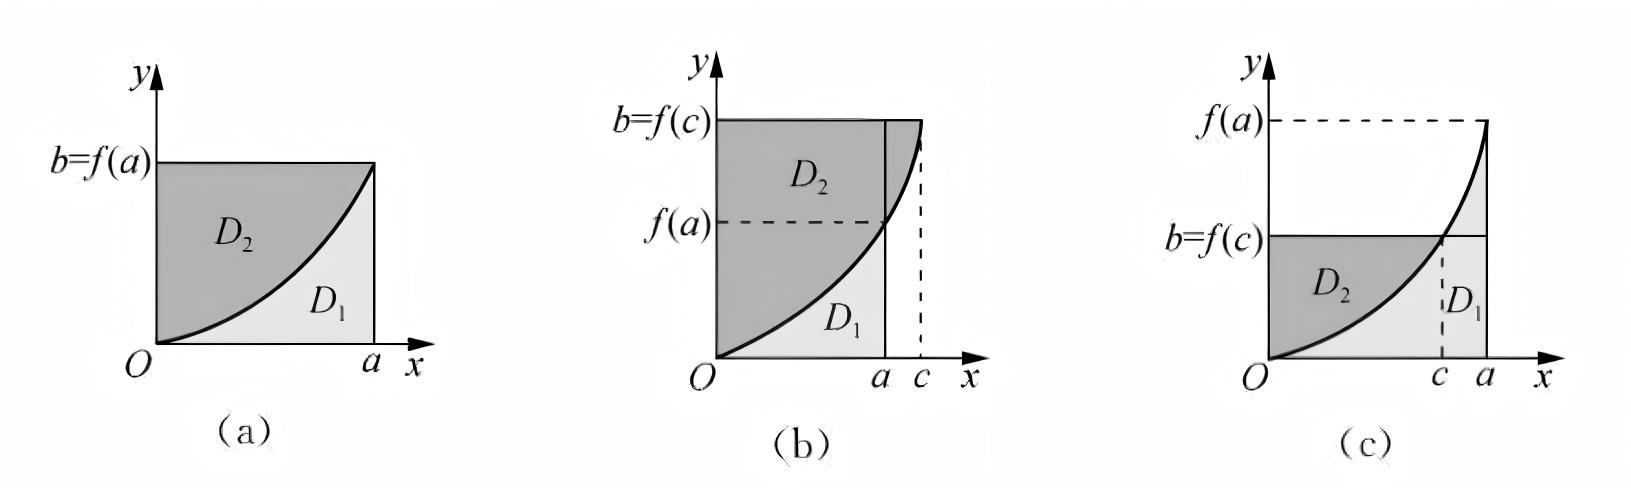
\includegraphics[width=0.7\linewidth]{figure/young}
	\end{center}
设 $f(a)=b$，取 $[0,a]$ 的划分：
	\[
	0 = x_0 < x_1 < \dots < x_n = a
	\]
	对应地令
	\[
	y_i = f(x_i)
	\]
	我们得到 $[0,b]$ 的划分
	\[
	0 = y_0 < y_1 < \dots < y_n = b
	\]
	那么
	\[
	\int_{0}^{a} f(x) \dd x = \sum_{i=1}^{n} y_{i-1} (x_i - x_{i-1}), \quad \int_{0}^{b} f^{-1}(x) \dd x = \sum_{i=1}^{n} x_i (y_i - y_{i-1})
	\]

	那么
	\begin{align*}
		\int_{0}^{a} f(x) \dd x + \int_{0}^{b} f^{-1}(x) \dd x
		&= \sum_{i=1}^{n} \left( x_i y_i - x_{i-1} y_{i-1} \right) \\
		&= x_n y_n - x_0 y_0 = ab
	\end{align*}
	
	若 $f(a) \neq b$，设 $f(T)=b$，令
	\[
	F(a) = \int_{0}^{a} f(x) \dd x + \int_{0}^{b} f^{-1}(x) \dd x - ab
	\]
	求导得
	\[
	F'(a) = f(a) - b
	\]
	
	\begin{itemize}
		\item 当 $a=T$ 时，$f(T)=b$，故 $F'(T)=0$
	 \item 当 $a>T$ 时，$f(a)>b$，故 $F'(a)>0$，$F(a)$ 单调递增
	\item 当 $a<T$ 时，$f(a)<b$，故 $F'(a)<0$，$F(a)$ 单调递减
	\end{itemize}
	
	故 $a=T$ 时 $F(a)$ 取得最小值，且 $F(T)=0$。因此 $\forall a$，有 $F(a) \geqslant 0$，也即
	\[
	\int_{0}^{a} f(x) \dd x + \int_{0}^{b} f^{-1}(x) \dd x \geqslant ab
	\]
\end{proof}
\begin{corollary}
	设 $p>1$，$q>1$ 且 $\dfrac{1}{p} + \dfrac{1}{q} = 1$，则 $\forall a,b \geqslant 0$，必有
	\[
	ab \leqslant \frac{a^p}{p} + \frac{b^q}{q}
	\]
\end{corollary}
\begin{proof}
	令 $y = x^{p-1}$，其反函数为 $x = y^{q-1}$。由Young不等式得
	\[
	\int_{0}^{a} x^{p-1} \dd x + \int_{0}^{b} x^{q-1} \dd x \geqslant ab
	\]
	计算积分即得
	\[
	ab \leqslant \frac{a^p}{p} + \frac{b^q}{q}
	\]
\end{proof}
\begin{corollary}
	（Hölder 不等式）设 $f,g \in C[a,b]$，$p,q>1$，且 $\dfrac{1}{p} + \dfrac{1}{q} = 1$，则
	\[
	\int_{a}^{b} |fg| \dd x \leqslant \left( \int_{a}^{b} |f|^p \dd x \right)^{\frac{1}{p}} \cdot \left( \int_{a}^{b} |g|^q \dd x \right)^{\frac{1}{q}}
	\]
	
若$p,q<1$，且 $\dfrac{1}{p} + \dfrac{1}{q} = 1$，则
\[
\int_{a}^{b} |fg| \dd x \geqslant \left( \int_{a}^{b} |f|^p \dd x \right)^{\frac{1}{p}} \cdot \left( \int_{a}^{b} |g|^q \dd x \right)^{\frac{1}{q}}
\]
	等号成立当且仅当$f^p(x)$与$g^q(x)$成比例时
\end{corollary}
\begin{proof}
	对任意 $\varphi(x),\psi(x) > 0$，$p,q>1$ 且 $\dfrac{1}{p} + \dfrac{1}{q} = 1$，有
	\[
	\varphi(x)\psi(x) \leqslant \frac{1}{p} \varphi(x)^p + \frac{1}{q} \psi(x)^q
	\]
	
	令
	\[
	\varphi(x) = \frac{|f(x)|}{\left( \displaystyle\int_{a}^{b} |f|^p \dd x \right)^{\frac{1}{p}}}, \quad
	\psi(x) = \frac{|g(x)|}{\left( \displaystyle\int_{a}^{b} |g|^q \dd x \right)^{\frac{1}{q}}}
	\]
	
	代入上述不等式，得
	\[
	\frac{|fg|}{\left( \displaystyle\int_{a}^{b} |f|^p \dd x \right)^{\frac{1}{p}} \left( \displaystyle\int_{a}^{b} |g|^q \dd x \right)^{\frac{1}{q}}}
	\leqslant \frac{|f|^p}{p \displaystyle\int_{a}^{b} |f|^p \dd x} + \frac{|g|^q}{q \displaystyle\int_{a}^{b} |g|^q \dd x}
	\]
	
	两边在 $[a,b]$ 上积分，整理后即得 Hölder 不等式。对称的证明类似
\end{proof}
\begin{corollary}
	(Minkowski不等式)$f,g\in\mathcal{R}[a,b]$且$f,g$的下界为正,则\[\sqrt[]{\int_{a}^{b}[f(x)+g(x)]^2\dd x}\leqslant \sqrt{\int_{a}^{b}f(x)\dd x}+\sqrt{\int_{a}^{b}g(x)\dd x}\]
\end{corollary}
\begin{proof}

	\[\begin{aligned}
			\int_{a}^{b}(f+g)^2\dd x&==2\int_{a}^{b}fg\dd x+\int_{a}^{b}f^2\dd x+\int_{a}^{b}g^2\dd x\\
			&\leqslant 2\sqrt{\int_{a}^{b}f^2\dd x\int_{a}^{b}g^2\dd x}+\int_{a}^{b}f^2\dd x+\int_{a}^{b}g^2\dd x\\
			&=(\sqrt[]{\int_{a}^{b}f^2\dd x}+\sqrt[]{\int_{a}^{b}g^2\dd x})^2
	\end{aligned}\]
\end{proof}
更进一步的，我们有
\begin{corollary}
	$f_i\in \mathcal{R}[a,b](i=1,\cdots,m)$，且下界为正，对$r>1$
	\[  \left[\int_{a}^{b}(f_1(x)+\cdots+f_m(x))^r\dd x\right]^{\frac{1}{r}}\leqslant (\int_{a}^{b}f_1^r(x)\dd x)^{\frac{1}{r}}+\cdots+(\int_{a}^{b}f_m^r(x)\dd x)^{\frac{1}{r}}  \]
	
	对$r<1$
	\[  \left[\int_{a}^{b}(f_1(x)+\cdots+f_m(x))^r\dd x\right]^{\frac{1}{r}}\geqslant (\int_{a}^{b}f_1^r(x)\dd x)^{\frac{1}{r}}+\cdots+(\int_{a}^{b}f_m^r(x)\dd x)^{\frac{1}{r}}  \]

\end{corollary}
%
% 第5节：中值定理
% !TEX root = ../../../main.tex
% 所属：第一部分：单变量分析学 / 第10章：一些定积分的问题
% 节：10.5 中值定理
% 正文按原文件顺序保存；由 ../chapter10.tex 调用。
\section{中值定理}

本节主要整理几道利用积分中值定理与 Rolle 中值定理的题目.

\begin{problem}
 设 $f(x)$ 在 $(0,1)$ 上可微，且满足
	\[
	f(1)-2\int_0^{\frac12}x f(x)\dd x=0.
	\]
	求证：在 $(0,1)$ 内至少有一点 $\xi$，使得
	\[
	f'(\xi)=-\frac{f(\xi)}{\xi}.
	\]
\end{problem}

\begin{proof}
	由积分中值定理，存在 $\eta\in\left(0,\dfrac12\right)$，使得
	\[
	\int_0^{\frac12}x f(x)\dd x=\frac12\eta f(\eta).
	\]
	因此
	\[
	f(1)=2\int_0^{\frac12}x f(x)\dd x=\eta f(\eta).
	\]
	令 $F(x)=x f(x)$，则
	\[
	F(1)=f(1)=\eta f(\eta)=F(\eta).
	\]
	于是对 $F(x)$ 在 $[\eta,1]$ 上应用 Rolle 中值定理，存在 $\xi\in(\eta,1)$，使得
	\[
	F'(\xi)=0.
	\]
	即
	\[
	f(\xi)+\xi f'(\xi)=0,
	\]
	所以
	\[
	f'(\xi)=-\frac{f(\xi)}{\xi}.
	\]
\end{proof}

\begin{problem}
设 $f(x)$ 在区间 $[0,1]$ 上连续，在 $(0,1)$ 上可导，满足
	\[
	f(1)=2\int_0^{\frac12}e^{1-x^2}f(x)\dd x.
	\]
	求证：存在一点 $\xi\in(0,1)$，使得
	\[
	f'(\xi)=2\xi f(\xi).
	\]
\end{problem}

\begin{proof}
	由题设两边同乘 $e^{-1}$ 得
	\[
	e^{-1}f(1)=2\int_0^{\frac12}e^{-x^2}f(x)\dd x.
	\]
	由积分中值定理，存在 $\eta\in\left(0,\dfrac12\right)$，使得
	\[
	2\int_0^{\frac12}e^{-x^2}f(x)\dd x=e^{-\eta^2}f(\eta).
	\]
	于是
	\[
	e^{-1}f(1)=e^{-\eta^2}f(\eta).
	\]
	令
	\[
	F(x)=e^{-x^2}f(x),
	\]
	则 $F(1)=F(\eta)$，由 Rolle 中值定理，存在 $\xi\in(\eta,1)$，使得
	\[
	F'(\xi)=0.
	\]
	又
	\[
	F'(x)=e^{-x^2}\left(f'(x)-2x f(x)\right),
	\]
	故
	\[
	f'(\xi)-2\xi f(\xi)=0,
	\]
	即
	\[
	f'(\xi)=2\xi f(\xi).
	\]
\end{proof}

\begin{problem}
设 $f(x)$ 在 $[0,1]$ 上连续，在 $(0,1)$ 内三次可微，并且满足条件：
	\[
	\int_0^{\frac14}f(t)\dd t=\frac14 f(0),
	\qquad
	\int_{\frac14}^{1}f(t)\dd t=\frac34 f(1).
	\]
	试证：若 $f(0)=f(1)$，则存在 $\xi\in(0,1)$，使得
	\[
	f'''(\xi)=0.
	\]
\end{problem}

\begin{proof}
	由积分中值定理，存在 $\xi_1\in\left(0,\dfrac14\right)$，使得
	\[
	\int_0^{\frac14}f(t)\dd t=\frac14 f(\xi_1).
	\]
	结合题设得
	\[
	f(\xi_1)=f(0).
	\]
	同理，存在 $\xi_2\in\left(\dfrac14,1\right)$，使得
	\[
	\int_{\frac14}^{1}f(t)\dd t=\frac34 f(\xi_2),
	\]
	从而
	\[
	f(\xi_2)=f(1).
	\]
	又 $f(0)=f(1)$，所以
	\[
	f(0)=f(\xi_1)=f(\xi_2)=f(1).
	\]
	于是分别在 $[0,\xi_1]$，$[\xi_1,\xi_2]$，$[\xi_2,1]$ 上应用 Rolle 中值定理，存在
	\[
	\eta_1\in(0,\xi_1),\qquad
	\eta_2\in(\xi_1,\xi_2),\qquad
	\eta_3\in(\xi_2,1),
	\]
	使得
	\[
	f'(\eta_1)=f'(\eta_2)=f'(\eta_3)=0.
	\]
	再对 $f'(x)$ 分别在 $[\eta_1,\eta_2]$ 与 $[\eta_2,\eta_3]$ 上应用 Rolle 中值定理，存在
	\[
	\delta_1\in(\eta_1,\eta_2),
	\qquad
	\delta_2\in(\eta_2,\eta_3),
	\]
	使得
	\[
	f''(\delta_1)=f''(\delta_2)=0.
	\]
	最后对 $f''(x)$ 在 $[\delta_1,\delta_2]$ 上应用 Rolle 中值定理，存在 $\xi\in(\delta_1,\delta_2)$，使得
	\[
	f'''(\xi)=0.
	\]
\end{proof}

\begin{problem}
	设函数 $f(x)$ 在 $[0,\pi]$ 上连续，且
	\[
	\int_0^\pi f(x)\dd x=0,
	\qquad
	\int_0^\pi f(x)\cos x\dd x=0.
	\]
	证明：在 $(0,\pi)$ 内至少存在两个不同的点 $\xi_1,\xi_2$，使得
	\[
	f(\xi_1)=f(\xi_2)=0.
	\]
\end{problem}

\begin{proof}
	令
	\[
	g(x)=\int_0^x f(t)\dd t,
	\qquad
	h(x)=\int_0^x g(t)\sin t\dd t.
	\]
	由题设知
	\[
	g(0)=g(\pi)=0,
	\qquad
	h(0)=0.
	\]
	又由分部积分，
	\[
	\begin{aligned}
		h(\pi)
		&=\int_0^\pi g(x)\sin x\dd x \\
		&=\left[-g(x)\cos x\right]_0^\pi+
		\int_0^\pi f(x)\cos x\dd x=0.
	\end{aligned}
	\]
	于是 $h(0)=h(\pi)=0$，由 Rolle 中值定理，存在 $\eta\in(0,\pi)$，使得
	\[
	h'(\eta)=g(\eta)\sin\eta=0.
	\]
	由于 $\eta\in(0,\pi)$，故 $\sin\eta>0$，从而
	\[
	g(\eta)=0.
	\]
	因此
	\[
	g(0)=g(\eta)=g(\pi)=0.
	\]
	分别对 $g(x)$ 在 $[0,\eta]$ 与 $[\eta,\pi]$ 上应用 Rolle 中值定理，存在
	\[
	\xi_1\in(0,\eta),
	\qquad
	\xi_2\in(\eta,\pi),
	\]
	使得
	\[
	g'(\xi_1)=g'(\xi_2)=0.
	\]
	又 $g'(x)=f(x)$，所以
	\[
	f(\xi_1)=f(\xi_2)=0.
	\]
	显然 $\xi_1\neq\xi_2$.
\end{proof}

%
% 第6节：定积分的数值积分-算法与编程
% !TEX root = ../../../main.tex
% 所属：第一部分：单变量分析学 / 第10章：一些定积分的问题
% 节：10.6 定积分的数值积分-算法与编程
% 正文按原文件顺序保存；由 ../chapter10.tex 调用。
\section{定积分的数值积分-算法与编程}
本节讨论若干常用的数值积分公式。基本思想是：在积分区间上先用多项式近似被积函数，再对这个多项式进行积分，从而得到原积分的近似值。

\subsection*{Newton--Cotes 求积公式}

将积分区间 $[a,b]$ 以步长
\[
h=\frac{b-a}{n}
\]
分成 $n$ 等份。

取分点
\[
x_i=a+ih,\qquad i=0,1,2,\dots,n.
\]

以这些分点为节点，作 $f(x)$ 的 Lagrange 插值多项式
\[
f(x)\approx p_n(x)
=\sum_{i=0}^{n}\left(\prod_{\substack{j=0\\j\ne i}}^{n}
\frac{x-x_j}{x_i-x_j}\right)f(x_i).
\]

对等式两边在 $[a,b]$ 上积分，得到
\[
\int_a^b f(x)\dd x
\approx \int_a^b p_n(x)\dd x
=(b-a)\sum_{i=0}^{n} C_i^{(n)}f(x_i).
\]

其中
\[
\begin{aligned}
	C_i^{(n)}
	&=\frac1{b-a}\int_a^b
	\prod_{\substack{j=0\\j\ne i}}^n\frac{x-x_j}{x_i-x_j}\dd x \\[4pt]
	&=\frac{h}{b-a}\int_0^n
	\prod_{\substack{j=0\\j\ne i}}^n\frac{t-j}{i-j}\dd t
	\qquad (x=a+th) \\[4pt]
	&=\frac1n\cdot \frac{(-1)^{n-i}}{i!(n-i)!}
	\int_0^n\prod_{\substack{j=0\\j\ne i}}^n(t-j)\dd t.
\end{aligned}
\]

这就是 $n$ 步 Newton--Cotes 求积公式。计算时需要 $n+1$ 个节点，相应的 $C_i^{(n)}$ 称为 Cotes 系数。它与积分区间和被积函数无关，只依赖于所取的节点个数，因此可以预先由多项式积分算出。

\begin{example}
	\textbf{梯形公式.}
	当 $n=1$ 时，由 Cotes 系数的性质，得到
	\[
	C_0^{(1)}=C_1^{(1)}=\frac12.
	\]因此
	\[
	\int_a^b f(x)\dd x
	\approx \frac{b-a}{2}\bigl[f(a)+f(b)\bigr].
	\]
	这称为梯形公式。
\end{example}
使用Python我们可以使用以下的代码进行计算
\begin{verbatim}
	import sympy
	from sympy import symbols, sympify, lambdify
	def trapezoidal_rule(f, a: float, b: float) -> float:
	return (b - a) / 2.0 * (f(a) + f(b))
	if __name__ == "__main__":
	x = symbols('x')
	expr_str = input("请输入函数表达式（例如：x**2 + sin(x)）：")
	expr = sympify(expr_str)
	a = float(input("请输入积分下限 a = "))
	b = float(input("请输入积分上限 b = "))
	f = lambdify(x, expr, modules="math")
	result = trapezoidal_rule(f, a, b)
	print(f"\n梯形公式近似值: {result:.10f}")
\end{verbatim}
\begin{example}
	\textbf{Simpson 公式.}
	当 $n=2$ 时，
	\[
	C_0^{(2)}=\frac14\int_0^2(t-1)(t-2)\dd t
	=\frac16=C_2^{(2)},
	\]
	因此得到 Simpson 公式
	\[
	\int_a^b f(x)\dd x
	\approx \frac{b-a}{6}
	\left[f(a)+4f\left(\frac{a+b}{2}\right)+f(b)\right].
	\]
\end{example}
使用Python我们可以使用以下的代码进行计算
\begin{verbatim}
	import sympy
	from sympy import symbols, sympify, lambdify
	def simpson_rule(f, a: float, b: float) -> float:
	mid = (a + b) / 2.0
	return (b - a) / 6.0 * (f(a) + 4.0 * f(mid) + f(b))
	if __name__ == "__main__":
	x = symbols('x')
	expr_str = input("请输入函数表达式（例如：x**2 + sin(x)）：")
	expr = sympify(expr_str)
	a = float(input("请输入积分下限 a = "))
	b = float(input("请输入积分上限 b = "))
	f = lambdify(x, expr, modules="math")
	result = simpson_rule(f, a, b)
	print(f"\nSimpson 公式近似值: {result:.10f}")
\end{verbatim}

\begin{example}
	\textbf{Cotes 公式.}
	当 $n=4$ 时，
	\[
	\begin{aligned}
		C_0^{(4)}
		&=\frac1{96}\int_0^4(t-1)(t-2)(t-3)(t-4)\dd t
		=\frac7{90}=C_4^{(4)},\\[4pt]
		C_1^{(4)}
		&=-\frac1{24}\int_0^4t(t-2)(t-3)(t-4)\dd t
		=\frac{32}{90}=C_3^{(4)},\\[4pt]
		C_2^{(4)}
		&=1-2\left(C_0^{(4)}+C_1^{(4)}\right)=\frac{12}{90}.
	\end{aligned}
	\]
	于是得到 Cotes 公式
	\[
	\int_a^b f(x)\dd x
	\approx \frac{b-a}{90}
	\left\{7\bigl[f(x_0)+f(x_4)\bigr]
	+32\bigl[f(x_1)+f(x_3)\bigr]+12f(x_2)\right\},
	\]
	其中
	\[
	x_i=\frac{(4-i)a+ib}{4},\qquad i=0,1,2,3,4.
	\]
	
\end{example}
使用Python我们可以使用以下的代码进行计算
\begin{verbatim}
	import sympy
	from sympy import symbols, sympify, lambdify
	def cotes_rule(f, a: float, b: float) -> float:
	n = 4
	x = [((n - i) * a + i * b) / n for i in range(n + 1)]
	C = [7/90, 32/90, 12/90, 32/90, 7/90]
	s = sum(C[i] * f(x[i]) for i in range(n + 1))
	return (b - a) * s
	if __name__ == "__main__":
	x = symbols('x')
	expr_str = input("请输入函数表达式（例如：x**2 + sin(x)）：")
	expr = sympify(expr_str)
	a = float(input("请输入积分下限 a = "))
	b = float(input("请输入积分上限 b = "))
	f = lambdify(x, expr, modules="math")
	result = cotes_rule(f, a, b)
	print(f"\nCotes 公式近似值: {result:.10f}")
\end{verbatim}


\subsection*{复化公式}

单一区间上的求积公式通常只利用少数节点。为了提高近似效果，可以先把 $[a,b]$ 划分为若干小区间，再在每个小区间上使用相同的求积公式，最后把各小区间的结果相加。这类公式称为复化求积公式。


	\textbf{复化梯形公式.}
	将 $[a,b]$ 以步长
	\[
	h=\frac{b-a}{m}
	\]
	作 $m$ 等分。

记
\[
x_i=a+ih,\qquad i=0,1,2,\dots,m.
\]

在每一个小区间 $[x_{i-1},x_i]$ 上使用梯形公式，得到
\[
\begin{aligned}
	\int_a^b f(x)\dd x
	&=\sum_{i=1}^{m}\int_{x_{i-1}}^{x_i}f(x)\dd x \\[2pt]
	&\approx \frac{h}{2}\sum_{i=1}^{m}
	\bigl[f(x_{i-1})+f(x_i)\bigr].
\end{aligned}
\]

记
\[
T_m^{(1)}
=\frac{h}{2}\left[f(a)+f(b)+2\sum_{i=1}^{m-1}f(x_i)\right],
\]
则称 $T_m^{(1)}$ 为将区间 $m$ 等分的复化梯形公式。

使用Python我们可以使用以下的代码进行计算
\begin{verbatim}
	import sympy
	from sympy import symbols, sympify, lambdify
	def composite_trapezoidal_rule(f, a: float, b: float, m: int) -> float:
	h = (b - a) / m
	s = f(a) + f(b)
	for i in range(1, m):
	s += 2.0 * f(a + i * h)
	return (h / 2.0) * s
	if __name__ == "__main__":
	x = symbols('x')
	expr_str = input("请输入函数表达式（例如：x**2 + sin(x)）：")
	expr = sympify(expr_str)
	a = float(input("请输入积分下限 a = "))
	b = float(input("请输入积分上限 b = "))
	m = int(input("请输入等分数 m = "))
	f = lambdify(x, expr, modules="math")
	result = composite_trapezoidal_rule(f, a, b, m)
	print(f"\n复化梯形公式近似值: {result:.10f}")
	
\end{verbatim}
	\textbf{复化 Simpson 公式.}
	记
	\[
	x_{i-\frac12}=\frac{x_{i-1}+x_i}{2}
	\]
	为区间 $[x_{i-1},x_i]$ 的中点。


在每个小区间上使用 Simpson 公式，可以得到复化 Simpson 公式
\[
\begin{aligned}
	T_m^{(2)}=S_m
	&=\frac{h}{6}\sum_{i=1}^{m}
	\left[f(x_{i-1})+4f\left(x_{i-\frac12}\right)+f(x_i)\right] \\[4pt]
	&=\frac{h}{6}\left[f(a)+f(b)
	+2\sum_{i=1}^{m-1}f(x_i)
	+4\sum_{i=1}^{m}f\left(x_{i-\frac12}\right)\right].
\end{aligned}
\]
使用Python我们可以使用以下的代码进行计算
\begin{verbatim}
	import sympy
	from sympy import symbols, sympify, lambdify
	def composite_simpson_rule(f, a: float, b: float, m: int) -> float:
	h = (b - a) / m
	s = f(a) + f(b)
	for i in range(1, m):
	s += 2.0 * f(a + i * h)
	for i in range(1, m + 1):
	s += 4.0 * f(a + (i - 0.5) * h)
	return (h / 6.0) * s
	if __name__ == "__main__":
	x = symbols('x')
	expr_str = input("请输入函数表达式（例如：x**2 + sin(x)）：")
	expr = sympify(expr_str)
	a = float(input("请输入积分下限 a = "))
	b = float(input("请输入积分上限 b = "))
	m = int(input("请输入等分数 m = "))
	f = lambdify(x, expr, modules="math")
	result = composite_simpson_rule(f, a, b, m)
	print(f"\n复化 Simpson 公式近似值: {result:.10f}")
\end{verbatim}
	\textbf{复化 Cotes 公式.}
	在每个小区间 $[x_{i-1},x_i]$ 上使用四等分的 Cotes 公式。令
	\[
	y_{i,r}=x_{i-1}+\frac{r}{4}h,
	\qquad r=0,1,2,3,4,
	\]


则复化 Cotes 公式可以写为
\[
\begin{aligned}
	C_m
	=\frac{h}{90}\sum_{i=1}^{m}
	\bigl\{&7\bigl[f(y_{i,0})+f(y_{i,4})\bigr]
	+32\bigl[f(y_{i,1})+f(y_{i,3})\bigr] \\
	&+12f(y_{i,2})\bigr\}.
\end{aligned}
\]
使用Python我们可以使用以下的代码进行计算
\begin{verbatim}
	import sympy
	from sympy import symbols, sympify, lambdify
	def composite_cotes_rule(f, a: float, b: float, m: int) -> float:
	h = (b - a) / m
	s = 0.0
	for i in range(1, m + 1):
	x0 = a + (i - 1) * h        # y_{i,0}
	x1 = x0 + h / 4.0           # y_{i,1}
	x2 = x0 + h / 2.0           # y_{i,2}
	x3 = x0 + 3.0 * h / 4.0     # y_{i,3}
	x4 = x0 + h                 # y_{i,4}
	s += 7.0 * (f(x0) + f(x4)) + 32.0 * (f(x1) + f(x3)) + 12.0 * f(x2)
	return (h / 90.0) * s
	if __name__ == "__main__":
	x = symbols('x')
	expr_str = input("请输入函数表达式（例如：x**2 + sin(x)）：")
	expr = sympify(expr_str)
	a = float(input("请输入积分下限 a = "))
	b = float(input("请输入积分上限 b = "))
	m = int(input("请输入等分数 m = "))
	f = lambdify(x, expr, modules="math")
	result = composite_cotes_rule(f, a, b, m)
	print(f"\n复化 Cotes 公式近似值: {result:.10f}")
\end{verbatim}
\subsection*{Romberg 方法}

把上面的外推思想推广到一般的 $T_m^{(k)}$。记
\[
T_m^{(k+1)}
=\frac{4^kT_{2m}^{(k)}-T_m^{(k)}}{4^k-1}.
\]

这就得到数值积分的 Romberg 方法。它的计算过程可以按如下图式进行：先取适当的初始值 $m$，再依次逐个计算。向下的箭头表示把区间再细化一半，向右的箭头表示外推。

\providecommand{\rombergstep}[1]{\tikz[baseline=(char.base)]{\node[draw,circle,inner sep=0.5pt,font=\scriptsize] (char) {#1};}}

\begin{figure}[H]
	\centering
	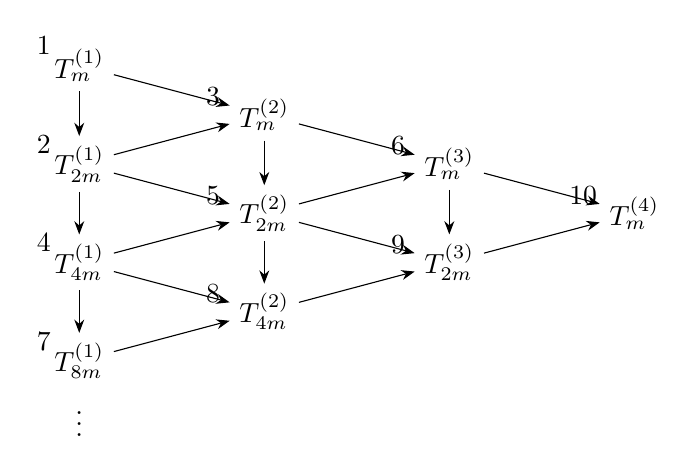
\begin{tikzpicture}[>=Stealth, node distance=1.15cm and 2.05cm]
		\node (a1) at (0,0) {$T_m^{(1)}$};
		\node (a2) at (0,-1.25) {$T_{2m}^{(1)}$};
		\node (a3) at (0,-2.50) {$T_{4m}^{(1)}$};
		\node (a4) at (0,-3.75) {$T_{8m}^{(1)}$};
		
		\node (b1) at (2.35,-0.625) {$T_m^{(2)}$};
		\node (b2) at (2.35,-1.875) {$T_{2m}^{(2)}$};
		\node (b3) at (2.35,-3.125) {$T_{4m}^{(2)}$};
		
		\node (c1) at (4.70,-1.25) {$T_m^{(3)}$};
		\node (c2) at (4.70,-2.50) {$T_{2m}^{(3)}$};
		
		\node (d1) at (7.05,-1.875) {$T_m^{(4)}$};
		
		\draw[->] (a1)--(a2);
		\draw[->] (a2)--(a3);
		\draw[->] (a3)--(a4);
		
		\draw[->] (a1)--(b1);
		\draw[->] (a2)--(b1);
		\draw[->] (a2)--(b2);
		\draw[->] (a3)--(b2);
		\draw[->] (a3)--(b3);
		\draw[->] (a4)--(b3);
		\draw[->] (b1)--(b2);
		\draw[->] (b2)--(b3);
		
		\draw[->] (b1)--(c1);
		\draw[->] (b2)--(c1);
		\draw[->] (b2)--(c2);
		\draw[->] (b3)--(c2);
		\draw[->] (c1)--(c2);
		
		\draw[->] (c1)--(d1);
		\draw[->] (c2)--(d1);
		
		\node at (-0.45,0.25) {\rombergstep{1}};
		\node at (-0.45,-1.00) {\rombergstep{2}};
		\node at (1.70,-0.40) {\rombergstep{3}};
		\node at (-0.45,-2.25) {\rombergstep{4}};
		\node at (1.70,-1.65) {\rombergstep{5}};
		\node at (4.05,-1.02) {\rombergstep{6}};
		\node at (-0.45,-3.50) {\rombergstep{7}};
		\node at (1.70,-2.90) {\rombergstep{8}};
		\node at (4.05,-2.27) {\rombergstep{9}};
		\node at (6.40,-1.65) {\rombergstep{10}};
		
		\node at (0,-4.45) {$\vdots$};
	\end{tikzpicture}
	\caption{Romberg 方法的计算顺序示意图}
\end{figure}

在实际计算中，一般从 $m=1$、$k=1$ 开始逐步计算 $T_m^{(k)}$。若对某个 $k$ 有 $|T_m^{(k)}-T_{m/2}^{(k)}|$ 小于预先设定的精度要求，就可把相应结果作为积分的近似值；否则继续把小区间长度缩小二分之一，计算出新的数值并继续比较。这种根据预置精度要求、在计算过程中自动把区间划分到合适程度的算法，称为自适应算法。
%
% 第7节：定积分的几何应用
% !TEX root = ../../../main.tex
% 所属：第一部分：单变量分析学 / 第10章：一些定积分的问题
% 节：10.7 定积分的几何应用
% 正文按原文件顺序保存；由 ../chapter10.tex 调用。
\section{定积分的几何应用}
本节整理定积分在几何问题中的若干基本应用。
\subsection*{平面图形的面积}

\begin{proposition}[直角坐标下的曲边梯形面积]
	设 $f$ 在 $[a,b]$ 上连续。
	\begin{enumerate}
		\item 若 $f(x)\geq 0$，则由 $y=f(x)$、$x=a$、$x=b$ 与 $x$ 轴围成的曲边梯形面积为
		\[
		S=\int_a^b f(x)\dd x .
		\]
		\item 若 $f(x)\leq 0$，则对应面积为
		\[
		S=-\int_a^b f(x)\dd x=\int_a^b \abs{f(x)}\dd x .
		\]
		\item 一般地，若 $f$ 在区间内可能变号，则面积为
		\[
		S=\int_a^b \abs{f(x)}\dd x .
		\]
	\end{enumerate}
\end{proposition}

\begin{proof}
	当 $f(x)\geq 0$ 时，面积由 Riemann 和
	\[
	\sum_{i=1}^n f(\xi_i)\Delta x_i
	\]
	的极限给出，因此为 $\displaystyle\int_a^b f(x)\dd x$。若 $f(x)\leq 0$，图形在 $x$ 轴下方，几何面积应取正值，故为 $-\displaystyle\int_a^b f(x)\dd x$。若 $f$ 有变号点，则把 $[a,b]$ 按变号点分成有限个小区间，在每段分别应用前两种情形，合并后得到
	\[
	S=\int_a^b \abs{f(x)}\dd x .
	\]
\end{proof}

\begin{figure}[H]
	\begin{center}
		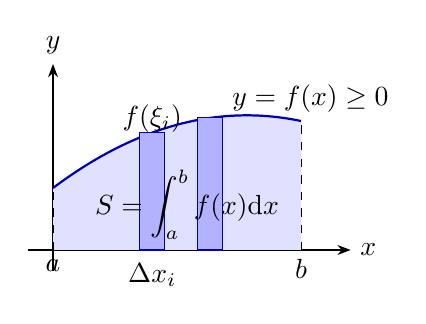
\begin{tikzpicture}[scale=1.05,>=Stealth]
			\draw[->] (-0.3,0) -- (3.6,0) node[right] {$x$};
			\draw[->] (0,-0.25) -- (0,2.25) node[above] {$y$};
			\fill[blue!12] (0,0) -- plot[domain=0:3,samples=80] ({\x},{0.75+0.75*\x-0.16*\x*\x}) -- (3,0) -- cycle;
			\draw[thick,blue!70!black,domain=0:3,samples=80] plot ({\x},{0.75+0.75*\x-0.16*\x*\x});
			\draw[dashed] (0,0) -- (0,{0.75});
			\draw[dashed] (3,0) -- (3,{0.75+0.75*3-0.16*9});
			\fill[blue!30] (1.05,0) rectangle (1.35,{0.75+0.75*1.2-0.16*1.2*1.2});
			\fill[blue!30] (1.75,0) rectangle (2.05,{0.75+0.75*1.9-0.16*1.9*1.9});
			\draw[blue!70!black] (1.05,0) rectangle (1.35,{0.75+0.75*1.2-0.16*1.2*1.2});
			\draw[blue!70!black] (1.75,0) rectangle (2.05,{0.75+0.75*1.9-0.16*1.9*1.9});
			\node[below] at (0,0) {$a$};
			\node[below] at (3,0) {$b$};
			\node[above right] at (2.05,1.55) {$y=f(x)\geq 0$};
			\node at (1.62,0.55) {$S=\displaystyle\int_a^b f(x)\dd x$};
			\node[below] at (1.20,-0.05) {$\Delta x_i$};
			\node[above] at (1.20,1.30) {$f(\xi_i)$};
		\end{tikzpicture}
	\end{center}
	\caption{曲边梯形面积：用小矩形面积之和逼近曲线下方区域。}
\end{figure}


\begin{proposition}[两条曲线之间的面积]
	设 $f,g$ 在 $[a,b]$ 上连续，且 $f(x)\geq g(x)$。则由 $y=f(x)$、$y=g(x)$、$x=a$ 与 $x=b$ 围成的平面图形面积为
	\[
	S=\int_a^b \bigl[f(x)-g(x)\bigr]\dd x .
	\]
	更一般地，若两曲线在区间内有交点，则应按交点分段；等价地可以写成
	\[
	S=\int_a^b \abs{f(x)-g(x)}\dd x .
	\]
\end{proposition}

\begin{proof}
	在每个小区间 $[x_{i-1},x_i]$ 上，面积近似为高为 $f(\xi_i)-g(\xi_i)$、宽为 $\Delta x_i$ 的小矩形面积，故
	\[
	S\approx \sum_{i=1}^n \bigl[f(\xi_i)-g(\xi_i)\bigr]\Delta x_i .
	\]
	令分割的最大长度趋于 $0$，由定积分定义得
	\[
	S=\int_a^b \bigl[f(x)-g(x)\bigr]\dd x .
	\]
	若上下关系发生改变，则在交点处分段，合并后得到绝对值形式。
\end{proof}

\begin{figure}[H]
	\begin{center}
		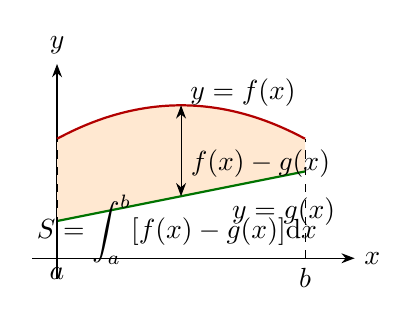
\begin{tikzpicture}[scale=1.05,>=Stealth]
			\draw[->] (-0.3,0) -- (3.6,0) node[right] {$x$};
			\draw[->] (0,-0.25) -- (0,2.35) node[above] {$y$};
			\fill[orange!18] plot[domain=0:3,samples=80] ({\x},{1.85-0.18*(\x-1.5)*(\x-1.5)}) --
			plot[domain=3:0,samples=80] ({\x},{0.45+0.20*\x}) -- cycle;
			\draw[thick,red!70!black,domain=0:3,samples=80] plot ({\x},{1.85-0.18*(\x-1.5)*(\x-1.5)});
			\draw[thick,green!45!black,domain=0:3,samples=80] plot ({\x},{0.45+0.20*\x});
			\draw[dashed] (0,0) -- (0,{1.85-0.18*2.25});
			\draw[dashed] (3,0) -- (3,{1.85-0.18*2.25});
			\draw[<->] (1.5,{0.45+0.20*1.5}) -- (1.5,{1.85});
			\node[right] at (1.5,1.15) {$f(x)-g(x)$};
			\node[above] at (2.25,1.72) {$y=f(x)$};
			\node[below right] at (2.0,0.85) {$y=g(x)$};
			\node[below] at (0,0) {$a$};
			\node[below] at (3,0) {$b$};
			\node at (1.45,0.35) {$S=\displaystyle\int_a^b [f(x)-g(x)]\dd x$};
		\end{tikzpicture}
	\end{center}
	\caption{两条曲线之间的面积：小矩形的高为上曲线与下曲线的函数值之差。}
\end{figure}


\begin{proposition}[参数方程下的面积]
	设曲线由参数方程
	\[
	x=x(t),\qquad y=y(t),\qquad t\in[\alpha,\beta]
	\]
	给出，其中 $x,y$ 连续可微，且 $x(t)$ 在 $[\alpha,\beta]$ 上单调。若曲线与 $x$ 轴围成的区域位于 $x$ 轴同侧，则面积可写为
	\[
	S=\int_{\alpha}^{\beta}\abs{y(t)x'(t)}\dd t .
	\]
	若已经知道 $x'(t)\geq 0$，则
	\[
	S=\int_{\alpha}^{\beta} y(t)x'(t)\dd t;
	\]
	若 $x'(t)\leq 0$，则
	\[
	S=-\int_{\alpha}^{\beta} y(t)x'(t)\dd t .
	\]
\end{proposition}
\begin{proposition}[极坐标下的面积]
	设平面曲线由极坐标方程
	\[
	r=r(\theta),\qquad \theta\in[\alpha,\beta]
	\]
	给出。若曲线在该角区间内围成的区域可由射线角度单调扫过，则面积为
	\[
	S=\frac12\int_{\alpha}^{\beta}r^2(\theta)\dd\theta .
	\]
\end{proposition}
\begin{figure}[H]
	\begin{center}
		\begin{tikzpicture}[scale=1.0,>=Stealth]
			\begin{scope}
				\draw[->] (-0.2,0) -- (3.3,0) node[right] {$x$};
				\draw[->] (0,-0.2) -- (0,2.4) node[above] {$y$};
				\fill[blue!12] (0.35,0) -- plot[domain=0:3,samples=80] ({0.35+\x},{0.55+0.55*sin(55*\x)+0.25*\x}) -- (3.35,0) -- cycle;
				\draw[thick,blue!70!black,domain=0:3,samples=80] plot ({0.35+\x},{0.55+0.55*sin(55*\x)+0.25*\x});
				\node[below] at (0.35,0) {$x(\alpha)$};
				\node[below] at (3.35,0) {$x(\beta)$};
				\node at (1.8,0.45) {$S=\displaystyle\int_\alpha^\beta |y(t)x'(t)|\dd t$};
				\node[above] at (1.8,2.15) {参数方程面积};
			\end{scope}
			\begin{scope}[xshift=5.2cm]
				\draw[->] (-0.2,0) -- (3.0,0) node[right] {$x$};
				\draw[->] (0,-0.2) -- (0,2.6) node[above] {$y$};
				\fill[green!18] (0,0) -- plot[domain=25:125,variable=\t,samples=120]
				({(1.65+0.28*sin(2*\t))*cos(\t)},{(1.65+0.28*sin(2*\t))*sin(\t)}) -- cycle;
				\draw[thick,green!45!black,domain=25:125,variable=\t,samples=120]
				plot ({(1.65+0.28*sin(2*\t))*cos(\t)},{(1.65+0.28*sin(2*\t))*sin(\t)});
				\draw[thick] (0,0) -- ({(1.65+0.28*sin(50))*cos(25)},{(1.65+0.28*sin(50))*sin(25)});
				\draw[thick] (0,0) -- ({(1.65+0.28*sin(250))*cos(125)},{(1.65+0.28*sin(250))*sin(125)});
				\draw[->] (0.75,0) arc (0:25:0.75);
				\draw[->] (0.95,0) arc (0:125:0.95);
				\node at (0.95,0.25) {$\alpha$};
				\node at (-0.45,1.08) {$\beta$};
				\node at (0.8,1.05) {$r(\theta)$};
				\node[above] at (0.95,2.35) {极坐标面积};
				\node at (1.1,-0.35) {$S=\displaystyle\frac12\int_\alpha^\beta r^2(\theta)\dd\theta$};
			\end{scope}
		\end{tikzpicture}
	\end{center}
	\caption{参数方程面积与极坐标面积的图形来源。左图来自变量代换 $\dd x=x'(t)\dd t$；右图来自小扇形面积 $\frac12 r^2\Delta\theta$。}
\end{figure}
\newpage

\subsection*{曲线弧长}

\begin{proposition}[显式方程的弧长]
	设 $f$ 在 $[a,b]$ 上连续可微。曲线 $y=f(x)$ 在 $[a,b]$ 上的弧长为
	\[
	L=\int_a^b \sqrt{1+\bigl(f'(x)\bigr)^2}\dd x .
	\]
	对应的弧长微分为
	\[
	\dd l=\sqrt{1+\bigl(f'(x)\bigr)^2}\dd x .
	\]
\end{proposition}

\begin{proof}
	取分割
	\[
	a=x_0<x_1<\cdots<x_n=b .
	\]
	在小区间 $[x_{i-1},x_i]$ 上，用两端点连线长度近似曲线弧长，则
	\[
	\Delta l_i\approx
	\sqrt{(x_i-x_{i-1})^2+\bigl(f(x_i)-f(x_{i-1})\bigr)^2} .
	\]
	由 Lagrange 中值定理，存在 $\xi_i\in(x_{i-1},x_i)$，使得
	\[
	f(x_i)-f(x_{i-1})=f'(\xi_i)(x_i-x_{i-1}).
	\]
	因此
	\[
	\Delta l_i\approx \sqrt{1+\bigl(f'(\xi_i)\bigr)^2}\Delta x_i .
	\]
	求和并令分割最大长度趋于 $0$，得到
	\[
	L=\int_a^b \sqrt{1+\bigl(f'(x)\bigr)^2}\dd x .
	\]
\end{proof}

\begin{figure}[H]
	\begin{center}
		\begin{tikzpicture}[scale=1.05,>=Stealth]
			\draw[->] (-0.2,0) -- (4.4,0) node[right] {$x$};
			\draw[->] (0,-0.2) -- (0,2.6) node[above] {$y$};
			\draw[thick,blue!70!black,domain=0:4,samples=120] plot ({\x},{0.55+0.33*\x+0.28*sin(90*\x)});
			\draw[red!70!black,thick] (0,{0.55}) -- (1,{0.55+0.33+0.28*sin(90)});
			\draw[red!70!black,thick] (1,{0.55+0.33+0.28*sin(90)}) -- (2,{0.55+0.66+0.28*sin(180)});
			\draw[red!70!black,thick] (2,{0.55+0.66+0.28*sin(180)}) -- (3,{0.55+0.99+0.28*sin(270)});
			\draw[red!70!black,thick] (3,{0.55+0.99+0.28*sin(270)}) -- (4,{0.55+1.32+0.28*sin(360)});
			\node[above] at (2.65,0.8) {$y=f(x)$};
			\node[below] at (2.3,0.65) {折线长度 $\longrightarrow$ 曲线弧长};
			\node at (2.25,2.35) {$L=\displaystyle\int_a^b\sqrt{1+[f'(x)]^2}\dd x$};
		\end{tikzpicture}
	\end{center}
	\caption{显式方程弧长：先用相邻分点连成的折线近似曲线，再令分割加细。}
\end{figure}


\begin{proposition}[参数方程的弧长]
	设曲线由
	\[
	x=x(t),\qquad y=y(t),\qquad t\in[\alpha,\beta]
	\]
	给出，其中 $x,y$ 连续可微。若曲线无重复地由参数扫过，则其弧长为
	\[
	L=\int_{\alpha}^{\beta}
	\sqrt{\bigl(x'(t)\bigr)^2+\bigl(y'(t)\bigr)^2}\dd t .
	\]
	对应的弧长微分为
	\[
	\dd l=\sqrt{\bigl(x'(t)\bigr)^2+\bigl(y'(t)\bigr)^2}\dd t .
	\]
\end{proposition}
\begin{proposition}[极坐标方程的弧长]
	设曲线由
	\[
	r=r(\theta),\qquad \theta\in[\alpha,\beta]
	\]
	给出，其中 $r$ 连续可微。则弧长为
	\[
	L=\int_{\alpha}^{\beta}
	\sqrt{r^2(\theta)+\bigl(r'(\theta)\bigr)^2}\dd\theta .
	\]
	对应的弧长微分为
	\[
	\dd l=\sqrt{r^2(\theta)+\bigl(r'(\theta)\bigr)^2}\dd\theta .
	\]
\end{proposition}
\begin{example}[椭圆周长]
	设椭圆
	\[
	\frac{x^2}{a^2}+\frac{y^2}{b^2}=1,
	\qquad a>b>0,
	\]
	取参数方程
	\[
	x=a\cos t,
	\qquad
	y=b\sin t,
	\qquad 0\leq t\leq 2\pi .
	\]
	则
	\[
	\begin{aligned}
		L
		&=\int_0^{2\pi}\sqrt{a^2\sin^2t+b^2\cos^2t}\dd t \\
		&=a\int_0^{2\pi}\sqrt{1-k^2\cos^2t}\dd t,
		\qquad k=\frac{\sqrt{a^2-b^2}}{a} \\
		&=4a\int_0^{\frac{\pi}{2}}\sqrt{1-k^2\sin^2u}\dd u .
	\end{aligned}
	\]
	若记
	\[
	E(k,\varphi)=\int_0^{\varphi}\sqrt{1-k^2\sin^2u}\dd u,
	\]
	则 $E(k,\varphi)$ 称为第二类不完全椭圆积分；若进一步记
	\[
	E(k)=E\left(k,\frac{\pi}{2}\right),
	\]
	则椭圆周长可写为
	\[
	L=4aE(k).
	\]
\end{example}

\subsection*{旋转体体积}

\begin{proposition}[已知截面积的体积]
	设立体在垂直于 $x$ 轴的截面面积为 $A(x)$，其中 $x\in[a,b]$。若 $A$ 在 $[a,b]$ 上连续，则立体体积为
	\[
	V=\int_a^b A(x)\dd x .
	\]
\end{proposition}

\begin{proof}
	取分割 $a=x_0<x_1<\cdots<x_n=b$。在小区间 $[x_{i-1},x_i]$ 内任取 $\xi_i$，小段体积近似为
	\[
	A(\xi_i)\Delta x_i .
	\]
	于是
	\[
	V\approx \sum_{i=1}^n A(\xi_i)\Delta x_i .
	\]
	令分割最大长度趋于 $0$，由定积分定义得到
	\[
	V=\int_a^b A(x)\dd x .
	\]
\end{proof}

\begin{figure}[H]
	\begin{center}
		\begin{tikzpicture}[scale=1.0,>=Stealth]
			\draw[->] (-0.2,0) -- (5.0,0) node[right] {$x$};
			\foreach \x/\h in {0.7/0.55,1.5/0.85,2.3/1.05,3.1/0.82,3.9/0.50}
			{
				\fill[blue!10] (\x,0) ellipse (0.18 and \h);
				\draw[blue!60!black] (\x,0) ellipse (0.18 and \h);
			}
			\draw[thick,blue!50!black] (0.7,0.55) .. controls (1.6,1.05) and (2.7,1.25) .. (3.9,0.50);
			\draw[thick,blue!50!black] (0.7,-0.55) .. controls (1.6,-1.05) and (2.7,-1.25) .. (3.9,-0.50);
			\draw[dashed] (0.7,-0.8) -- (0.7,0.8);
			\draw[dashed] (3.9,-0.8) -- (3.9,0.8);
			\node[below] at (0.7,-0.85) {$a$};
			\node[below] at (3.9,-0.85) {$b$};
			\node[above] at (2.3,1.25) {截面积 $A(x)$};
			\draw[<->] (2.3,-1.35) -- (2.75,-1.35);
			\node[below] at (2.52,-1.35) {$\Delta x$};
			\node at (2.45,-2.75) {$V=\displaystyle\int_a^b A(x)\dd x$};
		\end{tikzpicture}
	\end{center}
	\caption{已知截面积求体积：把立体切成许多薄片，小薄片体积近似为 $A(\xi_i)\Delta x_i$。}
\end{figure}


\begin{corollary}[绕 $x$ 轴旋转所得旋转体体积]
	若 $f$ 在 $[a,b]$ 上连续，且 $f(x)\geq 0$，则曲边梯形绕 $x$ 轴旋转所得旋转体的体积为
	\[
	V=\pi\int_a^b f^2(x)\dd x .
	\]
\end{corollary}

\begin{proof}
	垂直于 $x$ 轴的截面是半径为 $f(x)$ 的圆，所以
	\[
	A(x)=\pi f^2(x).
	\]
	代入截面积公式 $V=\int_a^b A(x)\dd x$，得到
	\[
	V=\pi\int_a^b f^2(x)\dd x .
	\]
\end{proof}

\begin{figure}[H]
	\begin{center}
		\begin{tikzpicture}[scale=1.0,>=Stealth]
			\begin{scope}
				\draw[->] (-0.2,0) -- (3.8,0) node[right] {$x$};
				\draw[->] (0,-0.2) -- (0,2.2) node[above] {$y$};
				\fill[purple!12] (0.3,0) -- plot[domain=0:3,samples=80] ({0.3+\x},{0.55+0.65*sin(45*\x)+0.22*\x}) -- (3.3,0) -- cycle;
				\draw[thick,purple!70!black,domain=0:3,samples=80] plot ({0.3+\x},{0.55+0.65*sin(45*\x)+0.22*\x});
				\node at (1.8,0.35) {绕 $x$ 轴旋转};
				\draw[->,thick] (1.8,-0.1) arc (-80:260:0.23 and 0.10);
			\end{scope}
			\begin{scope}[xshift=4.9cm]
				\draw[->] (-0.2,0) -- (3.8,0) node[right] {$x$};
				\draw[thick,purple!70!black] (0.3,0.65) .. controls (1.3,1.35) and (2.5,1.55) .. (3.3,1.05);
				\draw[thick,purple!70!black] (0.3,-0.65) .. controls (1.3,-1.35) and (2.5,-1.55) .. (3.3,-1.05);
				\foreach \x/\r in {0.7/0.82,1.7/1.35,2.7/1.28}
				{
					\fill[purple!12] (\x,0) ellipse (0.16 and \r);
					\draw[purple!60!black] (\x,0) ellipse (0.16 and \r);
				}
				\draw[<->] (1.7,0) -- (1.7,1.35);
				\node[right] at (1.7,0.68) {$f(x)$};
				\node at (1.9,-1.75) {$V=\displaystyle\pi\int_a^b f^2(x)\dd x$};
			\end{scope}
		\end{tikzpicture}
	\end{center}
	\caption{圆盘法：垂直于 $x$ 轴的截面是半径为 $f(x)$ 的圆，因此 $A(x)=\pi f^2(x)$。}
\end{figure}



	若旋转区域由 $y=f(x)$ 与 $y=g(x)$ 围成，且 $f(x)\geq g(x)\geq 0$，则绕 $x$ 轴旋转得到的截面为圆环，体积为
	\[
	V=\pi\int_a^b \left(f^2(x)-g^2(x)\right)\dd x .
	\]
	这一公式是圆盘法的直接推广。


\subsection*{旋转曲面面积}

\begin{proposition}[显式方程的旋转曲面面积]
	设 $f$ 在 $[a,b]$ 上连续可微。曲线 $y=f(x)$ 绕 $x$ 轴旋转一周所得曲面的面积为
	\[
	S=2\pi\int_a^b \abs{f(x)}\sqrt{1+\bigl(f'(x)\bigr)^2}\dd x .
	\]
	若 $f(x)\geq 0$，则可写成
	\[
	S=2\pi\int_a^b f(x)\sqrt{1+\bigl(f'(x)\bigr)^2}\dd x .
	\]
\end{proposition}

\begin{proof}
	取分割
	\[
	a=x_0<x_1<\cdots<x_n=b .
	\]
	在小区间 $[x_{k-1},x_k]$ 上，用连接两端点的线段代替曲线段。该线段绕 $x$ 轴旋转后得到圆台侧面。记
	\[
	\ell_k=\sqrt{(x_k-x_{k-1})^2+\bigl(f(x_k)-f(x_{k-1})\bigr)^2} .
	\]
	圆台侧面积近似为
	\[
	S_k=\pi\ell_k\bigl(\abs{f(x_k)}+\abs{f(x_{k-1})}\bigr).
	\]
	由中值定理，存在 $\xi_k\in(x_{k-1},x_k)$，使得
	\[
	\ell_k=\sqrt{1+\bigl(f'(\xi_k)\bigr)^2}\Delta x_k .
	\]
	因此
	\[
	S_k=\pi\sqrt{1+\bigl(f'(\xi_k)\bigr)^2}
	\bigl(\abs{f(x_k)}+\abs{f(x_{k-1})}\bigr)\Delta x_k .
	\]
	当分割充分细时，$\abs{f(x_k)}$ 与 $\abs{f(x_{k-1})}$ 都趋近于同一小区间内的函数值，于是
	\[
	S\approx 2\pi\sum_{k=1}^n
	\abs{f(\xi_k)}\sqrt{1+\bigl(f'(\xi_k)\bigr)^2}\Delta x_k .
	\]
	令分割最大长度趋于 $0$，得到
	\[
	S=2\pi\int_a^b \abs{f(x)}\sqrt{1+\bigl(f'(x)\bigr)^2}\dd x .
	\]
\end{proof}

\begin{figure}[H]
	\begin{center}
		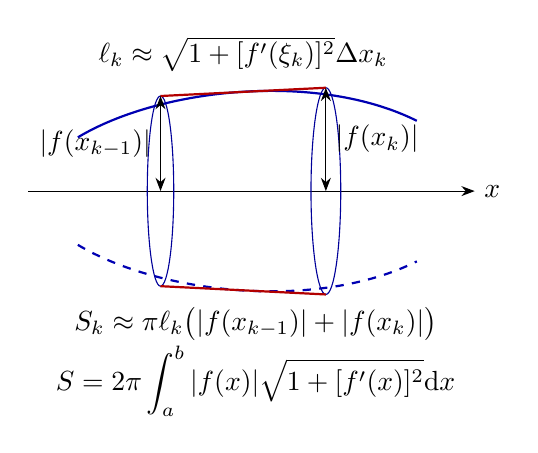
\begin{tikzpicture}[scale=1.05,>=Stealth]
			\draw[->] (-0.2,0) -- (5.2,0) node[right] {$x$};
			\draw[thick,blue!70!black] (0.4,0.65) .. controls (1.4,1.25) and (3.3,1.45) .. (4.5,0.85);
			\draw[thick,blue!70!black,dashed] (0.4,-0.65) .. controls (1.4,-1.25) and (3.3,-1.45) .. (4.5,-0.85);
			\draw[blue!60!black] (1.4,0) ellipse (0.16 and 1.15);
			\draw[blue!60!black] (3.4,0) ellipse (0.18 and 1.25);
			\draw[thick,red!70!black] (1.4,1.15) -- (3.4,1.25);
			\draw[thick,red!70!black] (1.4,-1.15) -- (3.4,-1.25);
			\draw[<->] (1.4,0) -- (1.4,1.15);
			\draw[<->] (3.4,0) -- (3.4,1.25);
			\node[left] at (1.4,0.58) {$|f(x_{k-1})|$};
			\node[right] at (3.4,0.63) {$|f(x_k)|$};
			\node[above] at (2.4,1.34) {$\ell_k\approx\sqrt{1+[f'(\xi_k)]^2}\Delta x_k$};
			\node at (2.55,-1.6) {$S_k\approx\pi\ell_k\bigl(|f(x_{k-1})|+|f(x_k)|\bigr)$};
			\node at (2.55,-2.3) {$S=\displaystyle2\pi\int_a^b |f(x)|\sqrt{1+[f'(x)]^2}\dd x$};
		\end{tikzpicture}
	\end{center}
	\caption{旋转曲面面积：小曲线段绕 $x$ 轴旋转后近似为圆台侧面。}
\end{figure}


\begin{corollary}[参数方程与极坐标下的旋转曲面面积]
	若曲线由
	\[
	x=x(t),\qquad y=y(t),\qquad t\in[T_1,T_2]
	\]
	给出，且绕 $x$ 轴旋转，则旋转曲面面积为
	\[
	S=2\pi\int_{T_1}^{T_2}
	\abs{y(t)}\sqrt{\bigl(x'(t)\bigr)^2+\bigl(y'(t)\bigr)^2}\dd t .
	\]
	若曲线由极坐标方程
	\[
	r=r(\theta),\qquad \theta\in[\alpha,\beta]
	\]
	给出，且绕极轴旋转，则由于 $y=r(\theta)\sin\theta$，有
	\[
	S=2\pi\int_{\alpha}^{\beta}
	\abs{r(\theta)\sin\theta}
	\sqrt{r^2(\theta)+\bigl(r'(\theta)\bigr)^2}\dd\theta .
	\]
\end{corollary}



下面把常用的面积、弧长、体积与旋转曲面面积公式统一整理如下。表中若涉及面积或半径，应根据具体图形关系取非负值；当图形位于标准位置时，可以省略绝对值。

\begin{center}
	\renewcommand{\arraystretch}{2.2}
	\small
	\resizebox{\textwidth}{!}{%
		\begin{tabular}{|c|c|c|c|}
			\hline
			& 直角坐标显式方程
			& 直角坐标参数方程
			& 极坐标方程 \\
			& $y=f(x),\ x\in[a,b]$
			& $\begin{cases}x=x(t),\\ y=y(t),\end{cases}\ t\in[T_1,T_2]$
			& $r=r(\theta),\ \theta\in[\alpha,\beta]$ \\
			\hline
			平面图形面积
			& $\displaystyle \int_a^b f(x)\dd x$
			& $\displaystyle \int_{T_1}^{T_2}\abs{y(t)x'(t)}\dd t$
			& $\displaystyle \frac12\int_{\alpha}^{\beta}r^2(\theta)\dd\theta$ \\
			\hline
			弧长的微分
			& $\displaystyle \dd l=\sqrt{1+\bigl(f'(x)\bigr)^2}\dd x$
			& $\displaystyle \dd l=\sqrt{\bigl(x'(t)\bigr)^2+\bigl(y'(t)\bigr)^2}\dd t$
			& $\displaystyle \dd l=\sqrt{r^2(\theta)+\bigl(r'(\theta)\bigr)^2}\dd\theta$ \\
			\hline
			曲线弧长
			& $\displaystyle \int_a^b\sqrt{1+\bigl(f'(x)\bigr)^2}\dd x$
			& $\displaystyle \int_{T_1}^{T_2}\sqrt{\bigl(x'(t)\bigr)^2+\bigl(y'(t)\bigr)^2}\dd t$
			& $\displaystyle \int_{\alpha}^{\beta}\sqrt{r^2(\theta)+\bigl(r'(\theta)\bigr)^2}\dd\theta$ \\
			\hline
			旋转体体积
			& $\displaystyle \pi\int_a^bf^2(x)\dd x$
			& $\displaystyle \pi\int_{T_1}^{T_2}y^2(t)\abs{x'(t)}\dd t$
			& $\displaystyle \frac{2\pi}{3}\int_{\alpha}^{\beta}r^3(\theta)\sin\theta\dd\theta$ \\
			\hline
			旋转曲面面积
			& $\displaystyle 2\pi\int_a^b\abs{f(x)}\sqrt{1+\bigl(f'(x)\bigr)^2}\dd x$
			& $\displaystyle 2\pi\int_{T_1}^{T_2}\abs{y(t)}\sqrt{\bigl(x'(t)\bigr)^2+\bigl(y'(t)\bigr)^2}\dd t$
			& $\displaystyle 2\pi\int_{\alpha}^{\beta}\abs{r(\theta)\sin\theta}\sqrt{r^2(\theta)+\bigl(r'(\theta)\bigr)^2}\dd\theta$ \\
			\hline
		\end{tabular}%
	}
\end{center}


	上表中的公式都有共同结构：
	\[
	\text{几何量}=\int \text{局部几何量的微分}.
	\]
	例如弧长公式来自
	\[
	\dd l=\sqrt{(\dd x)^2+(\dd y)^2},
	\]
	旋转曲面面积来自
	\[
	\dd S=2\pi\cdot \text{旋转半径}\cdot \dd l,
	\]
	旋转体体积来自
	\[
	\dd V=\text{截面积}\cdot \dd x .
	\]



%
% 第8节：Riemann--Stieltjes 积分
% !TEX root = ../../../main.tex
% 所属：第一部分：单变量分析学 / 第10章：一些定积分的问题
% 节：10.8 Riemann--Stieltjes 积分
% 正文按原文件顺序保存；由 ../chapter10.tex 调用。
\section{Riemann--Stieltjes 积分}

本节把前面关于 Riemann 积分的定义、Darboux 判别、基本性质以及几何应用，逐项改写为 Riemann--Stieltjes 积分的形式。核心变化只有一处：在 Riemann 积分中，区间长度为
\[
\Delta x_i=x_i-x_{i-1},
\]
而在 Stieltjes 积分中，区间的“长度”由一个单调函数 $\alpha$ 给出：
\[
\Delta \alpha_i=\alpha(x_i)-\alpha(x_{i-1}).
\]
这里需要注意的是我们并不要求$\alpha$连续

因此，Riemann 积分可以看作 $\alpha(x)=x$ 时的特殊情形。

除特别说明外，本节总假设 $\alpha:[a,b]\to\R$ 单调递增。于是对任意划分
\[
P:a=x_0<x_1<\cdots<x_n=b
\]
均有
\[
\Delta\alpha_i:=\alpha(x_i)-\alpha(x_{i-1})\geq 0.
\]

\begin{definition}
	设 $P:a=x_0<x_1<\cdots<x_n=b$ 是 $[a,b]$ 的一个划分，称
	\[
	\lambda(P)=\max_{1\leq i\leq n}(x_i-x_{i-1})
	\]
	为划分 $P$ 的模长。若 $\xi_i\in[x_{i-1},x_i]$，则称
	\[
	S(P,f,\alpha,\xi)=\sum_{i=1}^n f(\xi_i)\Delta\alpha_i
	\]
	为函数 $f$ 关于积分因子 $\alpha$ 的 Riemann--Stieltjes 和。
	
	若存在常数 $I$，使得对任意 $\eps>0$，存在 $\delta>0$，只要 $\lambda(P)<\delta$，并且任意选取 $\xi_i\in[x_{i-1},x_i]$，都有
	\[
	\left|\sum_{i=1}^n f(\xi_i)\Delta\alpha_i-I\right|<\eps,
	\]
	则称 $f$ 在 $[a,b]$ 上关于 $\alpha$ Riemann--Stieltjes 可积，记为
	\[
	f\in\mathcal R(\alpha;[a,b]),
	\]
	并记
	\[
	I=\int_a^b f(x)\dd\alpha(x).
	\]
\end{definition}

\begin{definition}
	设 $f$ 在 $[a,b]$ 上有界，$P:a=x_0<x_1<\cdots<x_n=b$ 是一个划分。在每个小区间 $[x_{i-1},x_i]$ 上记
	\[
	M_i=\sup_{x\in[x_{i-1},x_i]}f(x),\qquad
	m_i=\inf_{x\in[x_{i-1},x_i]}f(x).
	\]
	定义 Stieltjes-Darboux 大和与小和分别为
	\[
	\overline S_\alpha(P,f)=\sum_{i=1}^n M_i\Delta\alpha_i,
	\]
	\[
	\underline S_\alpha(P,f)=\sum_{i=1}^n m_i\Delta\alpha_i.
	\]
	称
	\[
	\omega_i=M_i-m_i
	\]
	为 $f$ 在 $[x_{i-1},x_i]$ 上的振幅。
\end{definition}

\begin{lemma}\label{lem:stieltjes-refinement}
	设 $f$ 在 $[a,b]$ 上有界，$\alpha$ 单调递增。若 $P'$ 是 $P$ 的加细，则
	\[
	\overline S_\alpha(P',f)\leq \overline S_\alpha(P,f),
	\qquad
	\underline S_\alpha(P',f)\geq \underline S_\alpha(P,f).
	\]
\end{lemma}

\begin{proof}
	只需证明在一个子区间中插入一个新分点的情形。设原来的一个子区间为 $[x_{k-1},x_k]$，插入新分点 $c$，其中
	\[
	x_{k-1}<c<x_k.
	\]
	记
	\[
	M_k=\sup_{[x_{k-1},x_k]}f,
	\]
	\[
	M_k'=\sup_{[x_{k-1},c]}f,
	\qquad
	M_k''=\sup_{[c,x_k]}f.
	\]
	显然
	\[
	M_k'\leq M_k,
	\qquad
	M_k''\leq M_k.
	\]
	因此大和在这一段上的变化满足
	\[
	\begin{aligned}
		& M_k'\bigl(\alpha(c)-\alpha(x_{k-1})\bigr)
		+M_k''\bigl(\alpha(x_k)-\alpha(c)\bigr)
		-M_k\bigl(\alpha(x_k)-\alpha(x_{k-1})\bigr) \\
		&\leq
		M_k\bigl(\alpha(c)-\alpha(x_{k-1})\bigr)
		+M_k\bigl(\alpha(x_k)-\alpha(c)\bigr)
		-M_k\bigl(\alpha(x_k)-\alpha(x_{k-1})\bigr)=0.
	\end{aligned}
	\]
	所以加细后大和不增。对小和同理：若
	\[
	m_k=\inf_{[x_{k-1},x_k]}f,
	\qquad
	m_k'=\inf_{[x_{k-1},c]}f,
	\qquad
	m_k''=\inf_{[c,x_k]}f,
	\]
	则
	\[
	m_k'\geq m_k,
	\qquad
	m_k''\geq m_k,
	\]
	从而加细后小和不减。
\end{proof}

\begin{proposition}\label{prop:stieltjes-darboux-bounds}
	设 $f$ 在 $[a,b]$ 上有界，$\alpha$ 单调递增。记
	\[
	M=\sup_{[a,b]}f,
	\qquad
	m=\inf_{[a,b]}f.
	\]
	则对任意两个划分 $P,Q$，有
	\[
	m\bigl(\alpha(b)-\alpha(a)\bigr)
	\leq \underline S_\alpha(P,f)
	\leq \overline S_\alpha(Q,f)
	\leq M\bigl(\alpha(b)-\alpha(a)\bigr).
	\]
\end{proposition}

\begin{proof}
	先由 $m\leq f(x)\leq M$ 得到每个小区间上
	\[
	m\leq m_i\leq M_i\leq M.
	\]
	由于 $\Delta\alpha_i\geq0$，故
	\[
	\underline S_\alpha(P,f)=\sum_i m_i\Delta\alpha_i
	\geq m\sum_i\Delta\alpha_i
	=m\bigl(\alpha(b)-\alpha(a)\bigr),
	\]
	并且
	\[
	\overline S_\alpha(Q,f)=\sum_j M_j\Delta\alpha_j
	\leq M\sum_j\Delta\alpha_j
	=M\bigl(\alpha(b)-\alpha(a)\bigr).
	\]
	为了证明中间不等式，取 $P$ 与 $Q$ 的公共加细 $P\vee Q$。由引理 \ref{lem:stieltjes-refinement}，有
	\[
	\underline S_\alpha(P,f)
	\leq \underline S_\alpha(P\vee Q,f)
	\leq \overline S_\alpha(P\vee Q,f)
	\leq \overline S_\alpha(Q,f).
	\]
	命题得证。
\end{proof}

\begin{definition}
	定义 $f$ 关于 $\alpha$ 的上 Stieltjes 积分与下 Stieltjes 积分为
	\[
	\overline{\int_a^b} f\dd\alpha
	=\inf_P \overline S_\alpha(P,f),
	\]
	\[
	\underline{\int_a^b} f\dd\alpha
	=\sup_P \underline S_\alpha(P,f),
	\]
	其中上下确界均对 $[a,b]$ 的全体划分 $P$ 取。
\end{definition}


\begin{theorem}\label{thm:stieltjes-darboux-criterion}
	设 $f$ 在 $[a,b]$ 上有界，$\alpha$ 单调递增。则 $f\in\mathcal R(\alpha;[a,b])$ 的充要条件是：对任意 $\eps>0$，存在 $\delta>0$，使得对任意划分 $P$，只要 $\lambda(P)<\delta$，就有
	\[
	\overline S_\alpha(P,f)-\underline S_\alpha(P,f)<\eps.
	\]
	等价地，
	\[
	\lim_{\lambda(P)\to0}\sum_{i=1}^n\omega_i\Delta\alpha_i=0.
	\]
\end{theorem}

\begin{proof}
	先证必要性。设
	\[
	\int_a^b f\dd\alpha=I.
	\]
	任给 $\eps>0$。由 Riemann--Stieltjes 可积的定义，存在 $\delta>0$，使得只要 $\lambda(P)<\delta$，任意 Stieltjes 和都满足
	\[
	\left|S(P,f,\alpha,\xi)-I\right|<\frac\eps4.
	\]
	固定这样的划分 $P$。记
	\[
	A=\alpha(b)-\alpha(a).
	\]
	若 $A=0$，则所有 $\Delta\alpha_i=0$，结论显然。以下设 $A>0$。由上确界、下确界定义，在每个小区间上可选取 $\xi_i',\xi_i''\in[x_{i-1},x_i]$，使得
	\[
	f(\xi_i')>M_i-\frac{\eps}{4A},
	\qquad
	f(\xi_i'')<m_i+\frac{\eps}{4A}.
	\]
	于是
	\[
	\overline S_\alpha(P,f)
	<\sum_i f(\xi_i')\Delta\alpha_i+\frac\eps4,
	\]
	\[
	\underline S_\alpha(P,f)
	>\sum_i f(\xi_i'')\Delta\alpha_i-\frac\eps4.
	\]
	两式相减并利用两个 Stieltjes 和都距 $I$ 小于 $\eps/4$，得
	\[
	\begin{aligned}
		\overline S_\alpha(P,f)-\underline S_\alpha(P,f)
		&<\left(\sum_i f(\xi_i')\Delta\alpha_i-I\right)
		+\left(I-\sum_i f(\xi_i'')\Delta\alpha_i\right)+\frac\eps2 \\
		&<\eps.
	\end{aligned}
	\]
	必要性得证。
	
	再证充分性。设对任意 $\eps>0$，存在 $\delta>0$，使得 $\lambda(P)<\delta$ 时
	\[
	\overline S_\alpha(P,f)-\underline S_\alpha(P,f)<\eps.
	\]
	要证明所有足够细的 Stieltjes 和收敛到同一极限。任取两个划分 $P,Q$，且
	\[
	\lambda(P)<\delta,
	\qquad
	\lambda(Q)<\delta.
	\]
	令 $R=P\vee Q$ 为公共加细。先比较 $P$ 上的任一 Stieltjes 和与 $R$ 上的某一 Stieltjes 和。对 $P$ 的一个子区间 $I_i=[x_{i-1},x_i]$，$R$ 把它分成若干小区间。无论这些小区间的标签怎样选取，它们对应的函数值都位于 $[m_i,M_i]$ 中，因此这一段上的和与 $f(\xi_i)\Delta\alpha_i$ 的差的绝对值不超过
	\[
	\omega_i\Delta\alpha_i.
	\]
	对所有 $i$ 求和，得到
	\[
	|S(P)-S(R)|\leq\sum_i\omega_i(P)\Delta\alpha_i
	=\overline S_\alpha(P,f)-\underline S_\alpha(P,f)<\eps.
	\]
	同理
	\[
	|S(Q)-S(R)|<\eps.
	\]
	因此
	\[
	|S(P)-S(Q)|\leq |S(P)-S(R)|+|S(R)-S(Q)|<2\eps.
	\]
	这说明当划分模长趋于 $0$ 时，全体 Stieltjes 和构成 Cauchy 族。由实数完备性，存在极限 $I$，且与划分和标签选取无关，即
	\[
	f\in\mathcal R(\alpha;[a,b]).
	\]
\end{proof}

\begin{corollary}\label{cor:stieltjes-oscillation-criterion}
	设 $f$ 在 $[a,b]$ 上有界，$\alpha$ 单调递增。则 $f\in\mathcal R(\alpha;[a,b])$ 的充要条件是：对任意 $\eps>0$，存在 $\delta>0$，使得只要 $\lambda(P)<\delta$，就有
	\[
	\sum_{i=1}^n\omega_i\Delta\alpha_i<\eps.
	\]
\end{corollary}

\begin{proof}
	由定义直接计算
	\[
	\begin{aligned}
		\overline S_\alpha(P,f)-\underline S_\alpha(P,f)
		&=\sum_{i=1}^n M_i\Delta\alpha_i-
		\sum_{i=1}^n m_i\Delta\alpha_i \\
		&=\sum_{i=1}^n (M_i-m_i)\Delta\alpha_i
		=\sum_{i=1}^n \omega_i\Delta\alpha_i.
	\end{aligned}
	\]
	代入定理 \ref{thm:stieltjes-darboux-criterion} 即得。
\end{proof}

\begin{corollary}\label{cor:stieltjes-one-partition-criterion}
	设 $f$ 在 $[a,b]$ 上有界，$\alpha$ 单调递增且连续。则 $f\in\mathcal R(\alpha;[a,b])$ 的充要条件是：对任意 $\eps>0$，存在划分 $P$，使得
	\[
	\sum_i\omega_i\Delta\alpha_i<\eps.
	\]
\end{corollary}

\begin{proof}
	必要性由推论 \ref{cor:stieltjes-oscillation-criterion} 立即得到。
	
	充分性只需把一个“好划分”推广为所有足够细划分。设 $P_0:a=y_0<y_1<\cdots<y_p=b$ 满足
	\[
	\sum_{j=1}^p\omega_j(P_0)\Delta\alpha_j<\frac\eps3.
	\]
	设 $|f(x)|\leq M$。由于 $\alpha$ 在有限个点 $y_1,\dots,y_{p-1}$ 处连续，可取 $\delta>0$，使得任意包含某个 $y_j$ 且长度小于 $2\delta$ 的区间 $J$ 都有
	\[
	\Delta\alpha(J)<\frac{\eps}{6M(p+1)}.
	\]
	同时令 $\delta$ 小于 $P_0$ 相邻分点距离的一半。若 $Q$ 是任意满足 $\lambda(Q)<\delta$ 的划分，令 $R=Q\vee P_0$。从 $Q$ 加细到 $R$ 时，只有那些含有 $P_0$ 内部分点的小区间会被切开，这样的小区间至多 $p-1$ 个；每个这样的区间对大和与小和的总影响不超过 $2M\Delta\alpha(J)$。故
	\[
	\begin{aligned}
		\overline S_\alpha(Q,f)-\underline S_\alpha(Q,f)
		&\leq \overline S_\alpha(R,f)-\underline S_\alpha(R,f)
		+2M\sum_J\Delta\alpha(J) \\
		&\leq \overline S_\alpha(P_0,f)-\underline S_\alpha(P_0,f)+\frac{\eps}{3}<\eps.
	\end{aligned}
	\]
	由推论 \ref{cor:stieltjes-oscillation-criterion}，$f\in\mathcal R(\alpha;[a,b])$。
\end{proof}

\begin{corollary}\label{cor:stieltjes-third-criterion}
	设 $f$ 在 $[a,b]$ 上有界，$\alpha$ 单调递增且连续。则 $f\in\mathcal R(\alpha;[a,b])$ 的一个等价表述为：对任意 $\eps>0$ 与 $\eta>0$，存在划分 $P$，使得振幅不小于 $\eta$ 的子区间的 $\alpha$-长度之和小于 $\eps$，即
	\[
	\sum_{\omega_i\geq\eta}\Delta\alpha_i<\eps.
	\]
\end{corollary}

\begin{proof}
	设 $m\leq f(x)\leq M$。若 $f\in\mathcal R(\alpha;[a,b])$，由推论 \ref{cor:stieltjes-oscillation-criterion}，对任意 $\eps\eta>0$，存在划分 $P$，使
	\[
	\sum_i\omega_i\Delta\alpha_i<\eps\eta.
	\]
	于是
	\[
	\eta\sum_{\omega_i\geq\eta}\Delta\alpha_i
	\leq \sum_{\omega_i\geq\eta}\omega_i\Delta\alpha_i
	\leq \sum_i\omega_i\Delta\alpha_i
	<\eps\eta,
	\]
	故
	\[
	\sum_{\omega_i\geq\eta}\Delta\alpha_i<\eps.
	\]
	
	反之，任给 $\eps>0$。取
	\[
	\eta=\frac{\eps}{2(\alpha(b)-\alpha(a)+1)},
	\qquad
	\eps' =\frac{\eps}{2(M-m+1)}.
	\]
	由条件，存在划分 $P$，使得
	\[
	\sum_{\omega_i\geq\eta}\Delta\alpha_i<\eps'.
	\]
	将求和分成两部分：
	\[
	\begin{aligned}
		\sum_i\omega_i\Delta\alpha_i
		&=\sum_{\omega_i\geq\eta}\omega_i\Delta\alpha_i
		+\sum_{\omega_i<\eta}\omega_i\Delta\alpha_i \\
		&\leq (M-m)\sum_{\omega_i\geq\eta}\Delta\alpha_i
		+\eta\sum_{\omega_i<\eta}\Delta\alpha_i \\
		&< (M-m)\eps'+\eta(\alpha(b)-\alpha(a))<\eps.
	\end{aligned}
	\]
	由推论 \ref{cor:stieltjes-one-partition-criterion} 可知 $f\in\mathcal R(\alpha;[a,b])$。
\end{proof}


\begin{proposition}\label{prop:continuous-integrand-stieltjes}
	若 $f\in C[a,b]$，$\alpha$ 单调递增，则
	\[
	f\in\mathcal R(\alpha;[a,b]).
	\]
\end{proposition}

\begin{proof}
	因 $f\in C[a,b]$，由闭区间连续函数一致连续性，对任意 $\eps>0$，存在 $\delta>0$，使得只要 $|x-y|<\delta$，就有
	\[
	|f(x)-f(y)|<\frac{\eps}{\alpha(b)-\alpha(a)+1}.
	\]
	取划分 $P$ 满足 $\lambda(P)<\delta$。则每个小区间上的振幅满足
	\[
	\omega_i<\frac{\eps}{\alpha(b)-\alpha(a)+1}.
	\]
	因此
	\[
	\sum_i \omega_i\Delta\alpha_i
	<\frac{\eps}{\alpha(b)-\alpha(a)+1}
	\sum_i\Delta\alpha_i
	\leq \eps.
	\]
	由推论 \ref{cor:stieltjes-oscillation-criterion}，$f$ 关于 $\alpha$ 可积。
\end{proof}

\begin{proposition}\label{prop:finite-discontinuities-alpha-continuous}
	若 $\alpha$ 单调递增且连续，$f$ 在 $[a,b]$ 上有界，并且只有有限多个不连续点，则
	\[
	f\in\mathcal R(\alpha;[a,b]).
	\]
\end{proposition}

\begin{proof}
	设 $f$ 的不连续点为 $c_1,\dots,c_N$，并设 $m\leq f(x)\leq M$。由于 $\alpha$ 连续且单调，函数
	\[
	\mu_\alpha([u,v])=\alpha(v)-\alpha(u)
	\]
	具有如下性质：当 $u,v$ 同时趋于 $c_j$ 时，
	\[
	\alpha(v)-\alpha(u)\to0.
	\]
	因此可取互不相交的小区间 $I_j=[c_j-\rho_j,c_j+\rho_j]\cap[a,b]$，使得
	\[
	\sum_{j=1}^N \mu_\alpha(I_j)<\frac{\eps}{2(M-m+1)}.
	\]
	在剩余的有限个闭区间上，$f$ 连续，故一致连续。于是可以继续加细划分，使得这些闭区间内每个小区间的振幅小于
	\[
	\frac{\eps}{2(\alpha(b)-\alpha(a)+1)}.
	\]
	于是总振幅和满足
	\[
	\begin{aligned}
		\sum_i \omega_i\Delta\alpha_i
		&=\sum_{I_i\subset \cup_j I_j}\omega_i\Delta\alpha_i
		+\sum_{I_i\cap \{c_1,\dots,c_N\}=\varnothing}\omega_i\Delta\alpha_i \\
		&\leq (M-m)\sum_{j=1}^N\mu_\alpha(I_j)
		+\frac{\eps}{2(\alpha(b)-\alpha(a)+1)}\bigl(\alpha(b)-\alpha(a)\bigr)
		<\eps.
	\end{aligned}
	\]
	故 $f\in\mathcal R(\alpha;[a,b])$。
\end{proof}
\begin{proposition}\label{prop:ordinary-reduction}
	若 $\alpha\in C^1[a,b]$，$\alpha'(x)\geq0$，且 $f\in C[a,b]$，则
	\[
	\int_a^b f(x)\dd\alpha(x)
	=\int_a^b f(x)\alpha'(x)\dd x.
	\]
\end{proposition}

\begin{proof}
	任取划分 $P:a=x_0<\cdots<x_n=b$ 及标签 $\xi_i\in[x_{i-1},x_i]$。由 Newton--Leibniz 公式，
	\[
	\Delta\alpha_i
	=\alpha(x_i)-\alpha(x_{i-1})
	=\int_{x_{i-1}}^{x_i}\alpha'(t)\dd t.
	\]
	于是
	\[
	\begin{aligned}
		\sum_i f(\xi_i)\Delta\alpha_i
		&=\sum_i f(\xi_i)\int_{x_{i-1}}^{x_i}\alpha'(t)\dd t \\
		&=\sum_i\int_{x_{i-1}}^{x_i}f(\xi_i)\alpha'(t)\dd t.
	\end{aligned}
	\]
	因为 $f$ 一致连续，且 $\alpha'$ 连续从而有界，设 $|\alpha'|\leq A$。当 $\lambda(P)$ 足够小时，对 $t\in[x_{i-1},x_i]$ 有
	\[
	|f(\xi_i)-f(t)|<\eta.
	\]
	所以
	\[
	\begin{aligned}
		\left|
		\sum_i f(\xi_i)\Delta\alpha_i
		-\int_a^b f(t)\alpha'(t)\dd t
		\right|
		&\leq \sum_i\int_{x_{i-1}}^{x_i}|f(\xi_i)-f(t)|\,|\alpha'(t)|\dd t \\
		&\leq A\eta(b-a).
	\end{aligned}
	\]
	令 $\eta\to0$ 即得结论。
\end{proof}
\begin{proposition}\label{prop:linear-integrand}
	设 $f,g\in\mathcal R(\alpha;[a,b])$，$k_1,k_2\in\R$。则
	\[
	k_1f+k_2g\in\mathcal R(\alpha;[a,b]),
	\]
	且
	\[
	\int_a^b (k_1f+k_2g)\dd\alpha
	=k_1\int_a^b f\dd\alpha+k_2\int_a^b g\dd\alpha.
	\]
\end{proposition}

\begin{proof}
	对任意子区间 $I$，有
	\[
	\omega_I(k_1f+k_2g)
	\leq |k_1|\omega_I(f)+|k_2|\omega_I(g).
	\]
	因此
	\[
	\sum_i\omega_i(k_1f+k_2g)\Delta\alpha_i
	\leq |k_1|\sum_i\omega_i(f)\Delta\alpha_i
	+|k_2|\sum_i\omega_i(g)\Delta\alpha_i.
	\]
	由 $f,g$ 的可积性与振幅判别可知 $k_1f+k_2g$ 可积。
	
	积分值的线性由 Stieltjes 和的线性直接推出：
	\[
	\sum_i (k_1f(\xi_i)+k_2g(\xi_i))\Delta\alpha_i
	=k_1\sum_i f(\xi_i)\Delta\alpha_i
	+k_2\sum_i g(\xi_i)\Delta\alpha_i.
	\]
	令 $\lambda(P)\to0$ 即得等式。
\end{proof}

\begin{proposition}\label{prop:linear-integrator}
	设 $\alpha,\beta$ 均单调递增，$f\in\mathcal R(\alpha;[a,b])\cap\mathcal R(\beta;[a,b])$，$c,d\geq0$。则
	\[
	f\in\mathcal R(c\alpha+d\beta;[a,b]),
	\]
	且
	\[
	\int_a^b f\dd(c\alpha+d\beta)
	=c\int_a^b f\dd\alpha+d\int_a^b f\dd\beta.
	\]
\end{proposition}

\begin{proof}
	对任意划分，
	\[
	\Delta(c\alpha+d\beta)_i
	=c\Delta\alpha_i+d\Delta\beta_i.
	\]
	因此
	\[
	\begin{aligned}
		\sum_i\omega_i(f)\Delta(c\alpha+d\beta)_i
		&=c\sum_i\omega_i(f)\Delta\alpha_i
		+d\sum_i\omega_i(f)\Delta\beta_i.
	\end{aligned}
	\]
	由 $f$ 分别关于 $\alpha$ 与 $\beta$ 可积，可知右端可任意小，所以 $f$ 关于 $c\alpha+d\beta$ 可积。积分值等式由 Stieltjes 和线性取极限得到。
\end{proof}

\begin{proposition}\label{prop:product-stieltjes}
	若 $f,g\in\mathcal R(\alpha;[a,b])$，则
	\[
	fg\in\mathcal R(\alpha;[a,b]).
	\]
\end{proposition}

\begin{proof}
	由于 $f,g$ 可积，二者有界。取 $M>0$，使得
	\[
	|f(x)|\leq M,
	\qquad
	|g(x)|\leq M.
	\]
	任取同一小区间内的 $x,y$，有
	\[
	\begin{aligned}
		|f(x)g(x)-f(y)g(y)|
		&\leq |f(x)|\,|g(x)-g(y)|+|g(y)|\,|f(x)-f(y)| \\
		&\leq M\omega(g)+M\omega(f).
	\end{aligned}
	\]
	故
	\[
	\omega(fg)\leq M\bigl(\omega(f)+\omega(g)\bigr).
	\]
	乘以 $\Delta\alpha_i$ 并求和，得
	\[
	\sum_i\omega_i(fg)\Delta\alpha_i
	\leq M\sum_i\omega_i(f)\Delta\alpha_i
	+M\sum_i\omega_i(g)\Delta\alpha_i.
	\]
	由 $f,g$ 的可积性，右端可任意小，故 $fg$ 可积。
\end{proof}

\begin{proposition}\label{prop:composition-stieltjes}
	设 $f\in\mathcal R(\alpha;[a,b])$，且
	\[
	A\leq f(x)\leq B.
	\]
	若 $\varphi\in C[A,B]$，则
	\[
	\varphi\circ f\in\mathcal R(\alpha;[a,b]).
	\]
\end{proposition}

\begin{proof}
	由于 $\varphi$ 在闭区间 $[A,B]$ 上连续，故一致连续且有界。设
	\[
	|\varphi(u)|\leq M.
	\]
	任给 $\eps>0$。由一致连续性，存在 $\eta>0$，使得只要 $|u-v|<\eta$，就有
	\[
	|\varphi(u)-\varphi(v)|<\frac{\eps}{2(\alpha(b)-\alpha(a)+1)}.
	\]
	由推论 \ref{cor:stieltjes-third-criterion}，存在划分 $P$，使得振幅 $\omega_i(f)\geq\eta$ 的子区间的 $\alpha$-长度之和小于
	\[
	\frac{\eps}{4M+1}.
	\]
	于是
	\[
	\begin{aligned}
		\sum_i\omega_i(\varphi\circ f)\Delta\alpha_i
		&=\sum_{\omega_i(f)<\eta}\omega_i(\varphi\circ f)\Delta\alpha_i
		+\sum_{\omega_i(f)\geq\eta}\omega_i(\varphi\circ f)\Delta\alpha_i \\
		&\leq \frac{\eps}{2(\alpha(b)-\alpha(a)+1)}\sum_i\Delta\alpha_i
		+2M\sum_{\omega_i(f)\geq\eta}\Delta\alpha_i
		<\eps.
	\end{aligned}
	\]
	由振幅判别，$\varphi\circ f$ 可积。
\end{proof}

\begin{proposition}\label{prop:monotonicity-stieltjes}
	若 $f,g\in\mathcal R(\alpha;[a,b])$，且对任意 $x\in[a,b]$ 有
	\[
	f(x)\geq g(x),
	\]
	则
	\[
	\int_a^b f\dd\alpha\geq \int_a^b g\dd\alpha.
	\]
\end{proposition}

\begin{proof}
	令 $h=f-g$，则 $h\in\mathcal R(\alpha;[a,b])$ 且 $h(x)\geq0$。对任意 Stieltjes 和有
	\[
	\sum_i h(\xi_i)\Delta\alpha_i\geq0,
	\]
	因为 $\Delta\alpha_i\geq0$。令 $\lambda(P)\to0$，得
	\[
	\int_a^b h\dd\alpha\geq0.
	\]
	再由线性性得到结论。
\end{proof}

\begin{proposition}\label{prop:absolute-value-stieltjes}
	若 $f\in\mathcal R(\alpha;[a,b])$，则
	\[
	|f|\in\mathcal R(\alpha;[a,b]),
	\]
	且
	\[
	\left|\int_a^b f\dd\alpha\right|
	\leq \int_a^b |f|\dd\alpha.
	\]
\end{proposition}

\begin{proof}
	由绝对值函数的不等式
	\[
	\bigl||u|-|v|\bigr|\leq |u-v|
	\]
	可得每个小区间上
	\[
	\omega(|f|)\leq\omega(f).
	\]
	故
	\[
	\sum_i\omega_i(|f|)\Delta\alpha_i
	\leq\sum_i\omega_i(f)\Delta\alpha_i.
	\]
	由 $f$ 的可积性知 $|f|$ 可积。
	
	又因
	\[
	-|f(x)|\leq f(x)\leq |f(x)|,
	\]
	由保序性得
	\[
	-\int_a^b |f|\dd\alpha
	\leq \int_a^b f\dd\alpha
	\leq \int_a^b |f|\dd\alpha.
	\]
	于是
	\[
	\left|\int_a^b f\dd\alpha\right|
	\leq \int_a^b |f|\dd\alpha.
	\]
\end{proof}

\begin{proposition}\label{prop:additivity-stieltjes}
	设 $c\in(a,b)$。则 $f\in\mathcal R(\alpha;[a,b])$ 当且仅当
	\[
	f\in\mathcal R(\alpha;[a,c])
	\quad\text{且}\quad
	f\in\mathcal R(\alpha;[c,b]).
	\]
	此时
	\[
	\int_a^b f\dd\alpha
	=\int_a^c f\dd\alpha+
	\int_c^b f\dd\alpha.
	\]
\end{proposition}

\begin{proof}
	若 $f$ 在 $[a,b]$ 上可积，则对任意 $\eps>0$，存在 $[a,b]$ 的划分 $P$，使得
	\[
	\sum_i\omega_i\Delta\alpha_i<\eps.
	\]
	若 $c$ 不是分点，就把 $c$ 加入划分。加细后振幅和不增。于是限制在 $[a,c]$ 与 $[c,b]$ 上的振幅和均不超过 $\eps$，故两段上均可积。
	
	反之，若两段上均可积，则分别取划分 $P_1,P_2$，使得
	\[
	\sum_{P_1}\omega_i\Delta\alpha_i<\frac\eps2,
	\qquad
	\sum_{P_2}\omega_i\Delta\alpha_i<\frac\eps2.
	\]
	合并两段划分得到 $[a,b]$ 上的划分 $P$，则
	\[
	\sum_P\omega_i\Delta\alpha_i<\eps.
	\]
	故 $f$ 在 $[a,b]$ 上可积。
	
	积分等式由 Stieltjes 和拆分得到：任意含 $c$ 的划分均有
	\[
	\sum_{[a,b]} f(\xi_i)\Delta\alpha_i
	=\sum_{[a,c]} f(\xi_i)\Delta\alpha_i
	+\sum_{[c,b]} f(\xi_i)\Delta\alpha_i.
	\]
	令模长趋于 $0$ 即得。
\end{proof}

\begin{proposition}\label{prop:first-mean-stieltjes}
	设 $f\in C[a,b]$，$g\in\mathcal R(\alpha;[a,b])$，且 $g$ 不变号。若 $\alpha$ 单调递增，则存在 $\xi\in[a,b]$，使得
	\[
	\int_a^b f(x)g(x)\dd\alpha(x)
	=f(\xi)\int_a^b g(x)\dd\alpha(x).
	\]
	特别地，取 $g\equiv1$，则存在 $\xi\in[a,b]$，使得
	\[
	\int_a^b f(x)\dd\alpha(x)
	=f(\xi)\bigl(\alpha(b)-\alpha(a)\bigr).
	\]
\end{proposition}

\begin{proof}
	不妨设 $g(x)\geq0$。因 $f$ 连续，存在最小值 $m$ 与最大值 $M$，满足
	\[
	m\leq f(x)\leq M.
	\]
	于是
	\[
	mg(x)\leq f(x)g(x)\leq Mg(x).
	\]
	由保序性得
	\[
	m\int_a^b g\dd\alpha
	\leq \int_a^b fg\dd\alpha
	\leq M\int_a^b g\dd\alpha.
	\]
	若 $\int_a^b g\dd\alpha=0$，则等式对任意 $\xi$ 成立。若 $\int_a^b g\dd\alpha>0$，则存在
	\[
	\eta\in[m,M]
	\]
	使
	\[
	\int_a^b fg\dd\alpha=\eta\int_a^b g\dd\alpha.
	\]
	由连续函数的介值性，存在 $\xi\in[a,b]$ 使得 $f(\xi)=\eta$。故结论成立。
\end{proof}



\begin{proposition}\label{prop:integration-by-parts-stieltjes}
	设 $f$ 与 $\alpha$ 均为 $[a,b]$ 上连续单调递增函数，则
	\[
	\int_a^b f\dd\alpha+\int_a^b \alpha\dd f
	=f(b)\alpha(b)-f(a)\alpha(a).
	\]
\end{proposition}

\begin{proof}
	取划分 $P:a=x_0<x_1<\cdots<x_n=b$。记
	\[
	f_i=f(x_i),
	\qquad
	\alpha_i=\alpha(x_i).
	\]
	对任意划分，有恒等式
	\[
	\begin{aligned}
		&\sum_{i=1}^n f(x_{i-1})\bigl(\alpha(x_i)-\alpha(x_{i-1})\bigr)
		+\sum_{i=1}^n \alpha(x_i)\bigl(f(x_i)-f(x_{i-1})\bigr) \\
		&=\sum_{i=1}^n \bigl(f_{i-1}\alpha_i-f_{i-1}\alpha_{i-1}+\alpha_i f_i-\alpha_i f_{i-1}\bigr) \\
		&=\sum_{i=1}^n(f_i\alpha_i-f_{i-1}\alpha_{i-1})
		=f(b)\alpha(b)-f(a)\alpha(a).
	\end{aligned}
	\]
	由于 $f,\alpha$ 连续，由命题 \ref{prop:continuous-integrand-stieltjes}，$f$ 关于 $\alpha$ 可积，$\alpha$ 关于 $f$ 可积。令 $\lambda(P)\to0$，左侧第一项趋于 $\int_a^b f\dd\alpha$，第二项趋于 $\int_a^b\alpha\dd f$，从而得到公式。
\end{proof}

\begin{proposition}\label{prop:change-variable-stieltjes}
	设 $\varphi:[A,B]\to[a,b]$ 连续、严格递增，且
	\[
	\varphi(A)=a,
	\qquad
	\varphi(B)=b.
	\]
	若 $f\in\mathcal R(\alpha;[a,b])$，则
	\[
	f\circ\varphi\in\mathcal R(\alpha\circ\varphi;[A,B]),
	\]
	且
	\[
	\int_a^b f(x)\dd\alpha(x)
	=\int_A^B f(\varphi(t))\dd(\alpha\circ\varphi)(t).
	\]
\end{proposition}

\begin{proof}
	任取 $[A,B]$ 的划分
	\[
	Q:A=t_0<t_1<\cdots<t_n=B.
	\]
	由 $\varphi$ 严格递增可得 $[a,b]$ 的划分
	\[
	P:a=\varphi(t_0)<\varphi(t_1)<\cdots<\varphi(t_n)=b.
	\]
	若 $\tau_i\in[t_{i-1},t_i]$，则 $\xi_i=\varphi(\tau_i)\in[\varphi(t_{i-1}),\varphi(t_i)]$。并且
	\[
	\Delta(\alpha\circ\varphi)_i
	=\alpha(\varphi(t_i))-\alpha(\varphi(t_{i-1}))
	=\Delta\alpha_i.
	\]
	因此两个 Stieltjes 和完全相同：
	\[
	\begin{aligned}
		\sum_i f(\varphi(\tau_i))\Delta(\alpha\circ\varphi)_i
		&=\sum_i f(\xi_i)\Delta\alpha_i.
	\end{aligned}
	\]
	当 $\lambda(Q)\to0$ 时，由 $\varphi$ 在闭区间上一致连续，$\lambda(P)\to0$。取极限即得变量代换公式。
\end{proof}

\begin{definition}
	设 $f\in\mathcal R(\alpha;[a,b])$。定义变上限 Stieltjes 积分函数
	\[
	F(x)=\int_a^x f(t)\dd\alpha(t),
	\qquad x\in[a,b].
	\]
\end{definition}

\begin{proposition}\label{prop:upper-limit-continuity-stieltjes}
	若 $f\in C[a,b]$，$\alpha$ 单调递增且连续，则
	\[
	F(x)=\int_a^x f(t)\dd\alpha(t)
	\]
	在 $[a,b]$ 上连续。
\end{proposition}

\begin{proof}
	由于 $f$ 连续，存在 $M>0$，使 $|f(x)|\leq M$。若 $x<y$，则
	\[
	\begin{aligned}
		|F(y)-F(x)|
		&=\left|\int_x^y f(t)\dd\alpha(t)\right| \\
		&\leq \int_x^y |f(t)|\dd\alpha(t)
		\leq M\bigl(\alpha(y)-\alpha(x)\bigr).
	\end{aligned}
	\]
	由于 $\alpha$ 连续，当 $y\to x$ 时
	\[
	\alpha(y)-\alpha(x)\to0.
	\]
	故 $F(y)\to F(x)$，即 $F$ 连续。
\end{proof}

%

%% ===== 第一部分：单变量分析学 / 第11章：一些反常积分的问题 =====
% !TEX root = ../../main.tex
\setchapterimage{figure/chapter11封面图.png}
\setchapterintro{}
\chapter{一些反常积分的问题}
% 第1节：一些习题
% !TEX root = ../../../main.tex
% 所属：第一部分：单变量分析学 / 第11章：一些反常积分的问题
% 节：11.1 一些习题
% 正文按原文件顺序保存；由 ../chapter11.tex 调用。
\section{一些习题}
本节整理反常积分的一组常用性质与判敛题。

\begin{proposition}（线性性）
	若
	\[
	\int_a^{+\infty} f(x)\dd x,
	\qquad
	\int_a^{+\infty} g(x)\dd x
	\]
	均收敛，且 $k_1,k_2\in\R$，则
	\[
	\int_a^{+\infty}\bigl[k_1f(x)+k_2g(x)\bigr]\dd x
	\]
	也收敛，并且
	\[
	\int_a^{+\infty}\bigl[k_1f(x)+k_2g(x)\bigr]\dd x
	=k_1\int_a^{+\infty} f(x)\dd x
	+k_2\int_a^{+\infty} g(x)\dd x.
	\]
\end{proposition}

\begin{proof}
	记
	\[
	I=\int_a^{+\infty}f(x)\dd x,
	\qquad
	J=\int_a^{+\infty}g(x)\dd x.
	\]
	由反常积分收敛的定义，
	\[
	\lim_{A\to+\infty}\int_a^A f(x)\dd x=I,
	\qquad
	\lim_{A\to+\infty}\int_a^A g(x)\dd x=J.
	\]
	对任意 $A>a$，由常义积分的线性性，
	\[
	\begin{aligned}
		\int_a^A\bigl[k_1f(x)+k_2g(x)\bigr]\dd x
		&=k_1\int_a^A f(x)\dd x+k_2\int_a^A g(x)\dd x.
	\end{aligned}
	\]
	令 $A\to+\infty$，由函数极限的线性性可得
	\[
	\lim_{A\to+\infty}\int_a^A\bigl[k_1f(x)+k_2g(x)\bigr]\dd x
	=k_1I+k_2J.
	\]
	故结论成立。
\end{proof}

\begin{example}
	证明
	\[
	\int_0^{+\infty}\frac{\ln x}{1+x^2}\dd x=0.
	\]
\end{example}

\begin{solution}
	先分解为
	\[
	\int_0^{+\infty}\frac{\ln x}{1+x^2}\dd x
	=\int_0^1\frac{\ln x}{1+x^2}\dd x
	+\int_1^{+\infty}\frac{\ln x}{1+x^2}\dd x.
	\]
	其中第一项在 $0$ 附近由 $|\ln x|$ 的可积性收敛；第二项在无穷远处由
	\[
	\frac{\ln x}{1+x^2}=O\left(\frac{\ln x}{x^2}\right)
	\]
	收敛。因此可以作变量代换 $x=1/t$：
	\[
	\begin{aligned}
		\int_1^{+\infty}\frac{\ln x}{1+x^2}\dd x
		&=\int_1^0\frac{\ln(1/t)}{1+1/t^2}\left(-\frac1{t^2}\right)\dd t  \\
		&=\int_0^1\frac{-\ln t}{1+t^2}\dd t.
	\end{aligned}
	\]
	于是
	\[
	\begin{aligned}
		\int_0^{+\infty}\frac{\ln x}{1+x^2}\dd x
		&=\int_0^1\frac{\ln x}{1+x^2}\dd x
		+\int_0^1\frac{-\ln x}{1+x^2}\dd x=0.
	\end{aligned}
	\]
\end{solution}

\begin{example}
	讨论
	\[
	\int_{-1}^{1}\frac1{x^3}\sin\frac1{x^2}\dd x
	\]
	的敛散性。
\end{example}

\begin{solution}
	只需考虑 $x=0$ 附近。对 $0<\varepsilon<1$，有
	\[
	\int_{\varepsilon}^{1}\frac1{x^3}\sin\frac1{x^2}\dd x
	=-\frac12\int_{\varepsilon}^{1}\sin\frac1{x^2}\dd\left(\frac1{x^2}\right)
	=\frac12\left[\cos\frac1{x^2}\right]_{\varepsilon}^{1}
	=\frac12\left(\cos 1-\cos\frac1{\varepsilon^2}\right).
	\]
	当 $\varepsilon\to0^+$ 时，$\cos(1/\varepsilon^2)$ 无极限，故
	\[
	\int_0^1\frac1{x^3}\sin\frac1{x^2}\dd x
	\]
	发散。原积分作为在 $0$ 有瑕点的反常积分也发散。
\end{solution}

\begin{proposition}（保序性）
	若
	\[
	\int_a^{+\infty} f(x)\dd x,
	\qquad
	\int_a^{+\infty} g(x)\dd x
	\]
	均收敛，并且对任意 $x\in[a,+\infty)$ 有 $f(x)\geq g(x)$，则
	\[
	\int_a^{+\infty}f(x)\dd x\geq \int_a^{+\infty}g(x)\dd x.
	\]
\end{proposition}

\begin{proof}
	对任意 $A>a$，由常义积分的保序性，有
	\[
	\int_a^{A}f(x)\dd x\geq \int_a^{A}g(x)\dd x.
	\]
	令 $A\to+\infty$，由于两边反常积分均收敛，便得到
	\[
	\int_a^{+\infty}f(x)\dd x\geq \int_a^{+\infty}g(x)\dd x.
	\]
\end{proof}

\begin{proposition}（区间可加性）
	设 $c\in[a,+\infty)$。若 $\displaystyle\int_a^{+\infty}f(x)\dd x$ 收敛，则
	\[
	\int_c^{+\infty}f(x)\dd x
	\]
	也收敛，并且
	\[
	\int_a^{+\infty}f(x)\dd x
	=\int_a^c f(x)\dd x+\int_c^{+\infty}f(x)\dd x.
	\]
	反之，若 $\displaystyle\int_c^{+\infty}f(x)\dd x$ 收敛，则 $\displaystyle\int_a^{+\infty}f(x)\dd x$ 收敛，且上式仍成立。
\end{proposition}

\begin{proof}
	对任意 $A>c$，常义积分区间可加性给出
	\[
	\int_a^A f(x)\dd x=\int_a^c f(x)\dd x+\int_c^A f(x)\dd x.
	\]
	若左端在 $A\to+\infty$ 时有极限，则右端第二项也有极限；若右端第二项有极限，则左端也有极限。取极限即得等式。
\end{proof}

\begin{example}
	反常积分的乘法可积性不成立。取
	\[
	f(x)=g(x)=\frac{\sin x}{\sqrt{x}},\qquad x\geq1.
	\]
	则
	\[
	\int_1^{+\infty}f(x)\dd x,
	\qquad
	\int_1^{+\infty}g(x)\dd x
	\]
	均收敛，但
	\[
	\int_1^{+\infty}f(x)g(x)\dd x
	=\int_1^{+\infty}\frac{\sin^2x}{x}\dd x
	\]
	发散。
\end{example}

\begin{solution}
	由 Dirichlet 判别法，$\displaystyle\int_1^{+\infty}\sin x\cdot x^{-1/2}\dd x$ 收敛，因为
	\[
	\int_1^A\sin x\dd x=\cos1-\cos A
	\]
	有界，且 $x^{-1/2}$ 单调趋于 $0$。
	
	另一方面，
	\[
	\sin^2x=\frac{1-\cos2x}{2},
	\]
	所以
	\[
	\int_1^A\frac{\sin^2x}{x}\dd x
	=\frac12\int_1^A\frac{\dd x}{x}
	-\frac12\int_1^A\frac{\cos2x}{x}\dd x.
	\]
	第二项由 Dirichlet 判别法收敛，而第一项 $\dfrac12\ln A$ 发散到 $+\infty$，故 $\displaystyle\int_1^{+\infty}\sin^2x/x\dd x$ 发散。
\end{solution}

\begin{proposition}（非负函数的 Cauchy 主值）
	设 $f(x)\geq0$，且 $f$ 在任意有限闭区间上可积。则
	\[
	(cpv)\int_{-\infty}^{+\infty}f(x)\dd x
	:=\lim_{A\to+\infty}\int_{-A}^{A}f(x)\dd x
	\]
	收敛当且仅当普通反常积分
	\[
	\int_{-\infty}^{+\infty}f(x)\dd x
	:=\int_{-\infty}^{0}f(x)\dd x+\int_0^{+\infty}f(x)\dd x
	\]
	收敛。此时二者相等。
\end{proposition}

\begin{proof}
	若普通反常积分收敛，则
	\[
	\int_{-A}^{A}f(x)\dd x
	=\int_{-A}^{0}f(x)\dd x+\int_0^{A}f(x)\dd x
	\]
	两项分别有有限极限，因此主值收敛，且极限等于普通反常积分。
	
	反过来，设
	\[
	F(A)=\int_{-A}^{A}f(x)\dd x
	\]
	当 $A\to+\infty$ 收敛。由于 $f\geq0$，$F(A)$ 关于 $A$ 单调递增，且有界，故对任意 $0<A'<A$，
	\[
	0\leq \int_{A'}^{A}f(x)\dd x\leq F(A)-F(A'),
	\]
	\[
	0\leq \int_{-A}^{-A'}f(x)\dd x\leq F(A)-F(A').
	\]
	由 $F(A)$ 收敛的 Cauchy 性，右端可任意小，于是
	\[
	\int_0^{+\infty}f(x)\dd x,
	\qquad
	\int_{-\infty}^{0}f(x)\dd x
	\]
	均收敛，故普通反常积分收敛。
\end{proof}

\begin{proposition}
	设 $\displaystyle\int_a^{+\infty}f(x)\dd x$ 收敛，并且
	\[
	\lim_{x\to+\infty}f(x)=A.
	\]
	若此极限存在，则必有 $A=0$。
\end{proposition}

\begin{proof}
	反证。若 $A>0$，取 $\eps=A/2$，则存在 $X\geq a$，使得 $x>X$ 时
	\[
	|f(x)-A|<\frac A2,
	\]
	从而 $f(x)>A/2$。于是对任意 $B>X$，
	\[
	\int_X^B f(x)\dd x\geq \frac A2(B-X)\to+\infty,
	\]
	这与 $\displaystyle\int_a^{+\infty}f(x)\dd x$ 收敛矛盾。若 $A<0$，则同理有
	\[
	\int_X^B f(x)\dd x\leq \frac A2(B-X)\to-\infty,
	\]
	也矛盾。因此 $A=0$。
\end{proof}

\textbf{非负函数反常积分的判敛练习}

\begin{problem}
	讨论下列非负函数反常积分的敛散性：
	\[
	\begin{array}{ll}
		(1)&\displaystyle \int_1^{+\infty}\frac{\dd x}{\sqrt{x^3-e^{-x}+\ln x+1}},\\[8pt]
		(2)&\displaystyle \int_1^{+\infty}\frac{\arctan x}{1+x^3}\dd x,\\[8pt]
		(3)&\displaystyle \int_0^{+\infty}\frac{\dd x}{1+x|\sin x|},\\[8pt]
		(4)&\displaystyle \int_1^{+\infty}\frac{x^p}{1+x^2}\dd x\qquad (p\in\R).
	\end{array}
	\]
\end{problem}

\begin{solution}
	(1) 当 $x\to+\infty$ 时，
	\[
	x^3-e^{-x}+\ln x+1\sim x^3,
	\]
	故
	\[
	\frac1{\sqrt{x^3-e^{-x}+\ln x+1}}\sim \frac1{x^{3/2}}.
	\]
	因为 $\displaystyle\int_1^{+\infty}x^{-3/2}\dd x$ 收敛，所以原积分收敛。
	
	(2) 因为 $0\leq\arctan x\leq \pi/2$，所以
	\[
	0\leq \frac{\arctan x}{1+x^3}\leq \frac{\pi/2}{1+x^3}\leq \frac{\pi/2}{x^3}.
	\]
	由比较判别法，原积分收敛。
	
	(3) 因为 $|\sin x|\leq1$，所以
	\[
	1+x|\sin x|\leq 1+x,
	\]
	从而
	\[
	\frac1{1+x|\sin x|}\geq \frac1{1+x}.
	\]
	由于 $\displaystyle\int_1^{+\infty}\frac{\dd x}{1+x}$ 发散，故原积分发散。
	
	(4) 当 $x\to+\infty$ 时，
	\[
	\frac{x^p}{1+x^2}\sim x^{p-2}.
	\]
	故原积分与 $\displaystyle\int_1^{+\infty}x^{p-2}\dd x$ 同敛散。于是
	\[
	p-2<-1\iff p<1
	\]
	时收敛；当 $p\geq1$ 时发散。
\end{solution}



\begin{problem}
	讨论下列反常积分的敛散性，包括绝对收敛、条件收敛和发散：
	\[
	\begin{array}{ll}
		(1)&\displaystyle \int_2^{+\infty}\frac{\ln\ln x}{\ln x}\sin x\dd x,\\[8pt]
		(2)&\displaystyle \int_1^{+\infty}\frac{\sin x}{x^p}\dd x\qquad(p\in\R),\\[8pt]
		(3)&\displaystyle \int_1^{+\infty}\frac{\sin x\arctan x}{x^p}\dd x\qquad(p\in\R),\\[8pt]
		(4)&\displaystyle \int_0^{+\infty}\sin(x^2)\dd x,\\[8pt]
		(5)&\displaystyle \int_a^{+\infty}\frac{P_m(x)}{Q_n(x)}\sin x\dd x.
	\end{array}
	\]
	其中 $P_m,Q_n$ 分别为 $m,n$ 次多项式，且 $Q_n$ 在 $[a,+\infty)$ 上无零点。
\end{problem}

\begin{solution}
	(1) 令
	\[
	h(x)=\frac{\ln\ln x}{\ln x}\qquad (x>e).
	\]
	则 $h(x)\to0$，且在充分大的区间上单调递减。又
	\[
	\int_2^A\sin x\dd x=\cos2-\cos A
	\]
	有界，因此由 Dirichlet 判别法，
	\[
	\int_2^{+\infty}\frac{\ln\ln x}{\ln x}\sin x\dd x
	\]
	收敛。
	
	接着证明它不绝对收敛。由于 $0<h(x)$ 且 $h(x)$ 最终单调下降，
	\[
	\int_2^A h(x)|\sin x|\dd x
	\geq \int_2^A h(x)\sin^2x\dd x.
	\]
	而
	\[
	\sin^2x=\frac{1-\cos2x}{2},
	\]
	故
	\[
	\int_2^A h(x)\sin^2x\dd x
	=\frac12\int_2^A h(x)\dd x-\frac12\int_2^A h(x)\cos2x\dd x.
	\]
	第二项由 Dirichlet 判别法收敛，而 $h(x)$ 对充分大 $x$ 满足 $h(x)\geq 1/x$，故 $\displaystyle\int_2^{+\infty}h(x)\dd x$ 发散。于是原积分条件收敛。
	
	(2) 若 $p>1$，则
	\[
	\int_1^{+\infty}\left|\frac{\sin x}{x^p}\right|\dd x
	\leq \int_1^{+\infty}\frac{\dd x}{x^p}<+\infty,
	\]
	故绝对收敛。若 $0<p\leq1$，则 $x^{-p}$ 单调趋于 $0$，由 Dirichlet 判别法知原积分收敛；但
	\[
	\int_1^{+\infty}\frac{|\sin x|}{x^p}\dd x
	\]
	发散，故条件收敛。若 $p\leq0$，则 $x^{-p}$ 不趋于 $0$，且在每个区间 $[2k\pi+\pi/6,2k\pi+5\pi/6]$ 上 $\sin x\geq1/2$，可由 Cauchy 不收敛原理推出积分发散。
	
	(3) 当 $x\to+\infty$ 时，$\arctan x\to\pi/2$。若 $p>1$，由比较判别法知绝对收敛。若 $0<p\leq1$，函数 $\arctan x/x^p$ 最终单调趋于 $0$，故由 Dirichlet 判别法知原积分收敛；又因 $\arctan x\geq c>0$ 对充分大的 $x$ 成立，绝对值积分与 $\displaystyle\int |\sin x|/x^p\dd x$ 同样发散，故条件收敛。若 $p\leq0$，被积函数不满足趋于 $0$ 的必要衰减，积分发散。
	
	(4) 令 $t=x^2$，则
	\[
	\int_1^{+\infty}\sin(x^2)\dd x
	=\frac12\int_1^{+\infty}\frac{\sin t}{\sqrt t}\dd t.
	\]
	右端由 Dirichlet 判别法收敛。另一方面
	\[
	\int_1^{+\infty}|\sin(x^2)|\dd x
	=\frac12\int_1^{+\infty}\frac{|\sin t|}{\sqrt t}\dd t
	\]
	发散，故原积分条件收敛。有限区间 $[0,1]$ 上无问题，因此整体条件收敛。
	
	(5) 当 $x\to+\infty$ 时，
	\[
	\frac{P_m(x)}{Q_n(x)}\sim Cx^{m-n}\qquad(C\neq0).
	\]
	若 $n-m>1$，则绝对值积分由 $p$-积分比较判别法收敛；若 $n-m=1$，则系数函数与 $C/x$ 同阶，由 Dirichlet 判别法原积分收敛，但绝对值积分发散，故条件收敛；若 $n-m<1$，则系数函数衰减不足，原积分发散。
\end{solution}

\textbf{有限端点瑕积分}

\begin{problem}
	讨论下列有限区间反常积分的敛散性：
	\[
	\begin{array}{ll}
		(1)&\displaystyle \int_0^1\frac{\dd x}{\sqrt[3]{x^2(1-x)}},\\[8pt]
		(2)&\displaystyle \int_0^1\frac{\ln x}{x^2-1}\dd x,\\[8pt]
		(3)&\displaystyle \int_0^{\pi/2}\frac{\dd x}{\cos^2x\sin^2x},\\[8pt]
		(4)&\displaystyle \int_0^{\pi/2}\frac{1-\cos x}{x^p}\dd x,\\[8pt]
		(5)&\displaystyle \int_0^1 |\ln x|^p\dd x,\\[8pt]
		(6)&\displaystyle \int_0^1x^{p-1}(1-x)^{q-1}\dd x,\\[8pt]
		(7)&\displaystyle \int_0^1x^{p-1}(1-x)^{q-1}|\ln x|\dd x.
	\end{array}
	\]
\end{problem}

\begin{solution}
	(1) 当 $x\to0^+$ 时，
	\[
	\frac1{\sqrt[3]{x^2(1-x)}}\sim x^{-2/3},
	\]
	当 $x\to1^-$ 时，
	\[
	\frac1{\sqrt[3]{x^2(1-x)}}\sim (1-x)^{-1/3}.
	\]
	两端幂指数均小于 $1$，故积分收敛。
	
	(2) 当 $x\to1^-$ 时，
	\[
	\lim_{x\to1^-}\frac{\ln x}{x^2-1}=\frac12.
	\]
	当 $x\to0^+$ 时，$x^2-1\to-1$，故被积函数与 $-\ln x$ 同阶，而 $\displaystyle\int_0^1|\ln x|\dd x$ 收敛。因此积分收敛。
	
	(3) 当 $x\to0^+$ 时，$\sin x\sim x$，$\cos x\to1$，故
	\[
	\frac1{\cos^2x\sin^2x}\sim \frac1{x^2}.
	\]
	$p=2\geq1$，故在 $0$ 端发散，原积分发散。
	
	(4) 当 $x\to0^+$ 时，
	\[
	1-\cos x\sim \frac{x^2}{2},
	\]
	所以
	\[
	\frac{1-\cos x}{x^p}\sim \frac12x^{2-p}.
	\]
	该函数在 $0$ 端可积当且仅当 $2-p>-1$，即 $p<3$。故当 $p<3$ 时收敛，当 $p\geq3$ 时发散。
	
	(5) 在 $0$ 端，令 $x=e^{-t}$，则 $t\to+\infty$，且
	\[
	\int_0^{1/2}|\ln x|^p\dd x
	=\int_{\ln2}^{+\infty} t^p e^{-t}\dd t,
	\]
	总是收敛。在 $1$ 端，$|\ln x|\sim 1-x$，故
	\[
	|\ln x|^p\sim (1-x)^p.
	\]
	因此积分收敛当且仅当 $p>-1$。
	
	(6) 当 $x\to0^+$ 时，被积函数与 $x^{p-1}$ 同阶；当 $x\to1^-$ 时，被积函数与 $(1-x)^{q-1}$ 同阶。故积分收敛当且仅当
	\[
	p>0,
	\qquad
	q>0.
	\]
	
	(7) 当 $x\to0^+$ 时，需要判断 $x^{p-1}|\ln x|$ 的可积性，它当且仅当 $p>0$ 时收敛；当 $x\to1^-$ 时，$|\ln x|\sim1-x$，故被积函数与
	\[
	(1-x)^q
	\]
	同阶，因此在 $1$ 端收敛当且仅当 $q>-1$。综上，积分收敛当且仅当
	\[
	p>0,
	\qquad
	q>-1.
	\]
\end{solution}

\newpage

\begin{problem}
	讨论下列反常积分的敛散性：
	\[
	\begin{array}{ll}
		(1)&\displaystyle \int_0^{1}\frac{x^{p-1}-x^{q-1}}{\ln x}\dd x\qquad(p,q\in\R),\\[8pt]
		(2)&\displaystyle \int_0^{+\infty}\frac{\dd x}{\sqrt[3]{x(x-1)^2(x-2)}},\\[8pt]
		(3)&\displaystyle \int_0^{+\infty}\frac{\ln(1+x)}{x^p}\dd x,\\[8pt]
		(4)&\displaystyle \int_0^{+\infty}\frac{\arctan x}{x^p}\dd x,\\[8pt]
		(5)&\displaystyle \int_0^{\pi/2}\frac{\sqrt{\tan x}}{x^p}\dd x,\\[8pt]
		(6)&\displaystyle \int_0^{+\infty}x^{p-1}e^{-x}\dd x,\\[8pt]
		(7)&\displaystyle \int_0^{+\infty}\frac{\dd x}{x^p+x^q},\\[8pt]
		(8)&\displaystyle \int_2^{+\infty}\frac{\dd x}{x^p\ln^qx}.
	\end{array}
	\]
\end{problem}

\begin{solution}
	(1) 若 $p=q$，则被积函数恒为 $0$，积分收敛。若 $p\neq q$，在 $x=1$ 附近，由 $x^r=1+r(x-1)+o(x-1)$ 与 $\ln x\sim x-1$，有
	\[
	\frac{x^{p-1}-x^{q-1}}{\ln x}\to p-q,
	\]
	故 $x=1$ 不是本质瑕点，只需考察 $0$ 端。令 $x=e^{-t}$，则 $t\to+\infty$，并且
	\[
	\int_0^{1/2}\frac{x^{p-1}-x^{q-1}}{\ln x}\dd x
	=\int_{\ln2}^{+\infty}\frac{e^{-pt}-e^{-qt}}{t}\dd t.
	\]
	因此当 $p>0$ 且 $q>0$ 时，右端由指数衰减控制而收敛；若 $p\leq0$ 或 $q\leq0$，且 $p\neq q$，则其中至少有一项在无穷远处不衰减或增长，不能由另一项抵消，故发散。综上，该积分收敛当且仅当
	\[
	p=q,
	\quad\text{或}\quad
	p>0,\ q>0.
	\]
	
	(2) 被积函数在 $0,1,2,+\infty$ 处可能出现问题。逐点比较：
	\[
	x\to0^+:\frac1{\sqrt[3]{x(x-1)^2(x-2)}}=O(x^{-1/3}),
	\]
	\[
	x\to1:\frac1{\sqrt[3]{x(x-1)^2(x-2)}}=O(|x-1|^{-2/3}),
	\]
	\[
	x\to2:\frac1{\sqrt[3]{x(x-1)^2(x-2)}}=O(|x-2|^{-1/3}),
	\]
	并且
	\[
	x\to+\infty:\frac1{\sqrt[3]{x(x-1)^2(x-2)}}=O(x^{-4/3}).
	\]
	所有相应幂指数均满足可积条件，故积分收敛。
	
	(3) 当 $x\to0^+$ 时，$\ln(1+x)\sim x$，故
	\[
	\frac{\ln(1+x)}{x^p}\sim x^{1-p},
	\]
	在 $0$ 端收敛当且仅当 $p<2$。当 $x\to+\infty$ 时，需考察 $\ln x/x^p$，它在无穷远处收敛当且仅当 $p>1$。故原积分收敛当且仅当
	\[
	1<p<2.
	\]
	
	(4) 当 $x\to0^+$ 时，$\arctan x\sim x$，故 $p<2$ 是 $0$ 端收敛条件；当 $x\to+\infty$ 时，$\arctan x\to\pi/2$，故需要 $p>1$。因此收敛当且仅当
	\[
	1<p<2.
	\]
	
	(5) 当 $x\to0^+$ 时，$\tan x\sim x$，所以
	\[
	\frac{\sqrt{\tan x}}{x^p}\sim x^{1/2-p},
	\]
	在 $0$ 端收敛当且仅当 $1/2-p>-1$，即 $p<3/2$。当 $x\to\pi/2^-$ 时，$\tan x\sim(\pi/2-x)^{-1}$，故
	\[
	\sqrt{\tan x}=O\bigl((\pi/2-x)^{-1/2}\bigr),
	\]
	该端总是可积。因此原积分收敛当且仅当
	\[
	p<\frac32.
	\]
	
	(6) 当 $x\to0^+$ 时，$e^{-x}\to1$，故被积函数与 $x^{p-1}$ 同阶；在 $+\infty$ 端，由指数函数衰减可知总是收敛。因此积分收敛当且仅当
	\[
	p>0.
	\]
	
	(7) 当 $x\to0^+$ 时，$x^p+x^q$ 由 $x^{\min\{p,q\}}$ 主导；当 $x\to+\infty$ 时，由 $x^{\max\{p,q\}}$ 主导。因此
	\[
	\frac1{x^p+x^q}
	\]
	在 $0$ 端收敛当且仅当 $\min\{p,q\}<1$，在 $+\infty$ 端收敛当且仅当 $\max\{p,q\}>1$。故原积分收敛当且仅当
	\[
	\min\{p,q\}<1<\max\{p,q\}.
	\]
	
	(8) 令 $t=\ln x$，则 $\dd t=\dd x/x$，并且
	\[
	\int_2^{+\infty}\frac{\dd x}{x^p\ln^qx}
	=\int_{\ln2}^{+\infty}\frac{e^{(1-p)t}}{t^q}\dd t.
	\]
	若 $p>1$，指数项衰减，积分收敛；若 $p<1$，指数项增长，积分发散；若 $p=1$，则化为
	\[
	\int_{\ln2}^{+\infty}\frac{\dd t}{t^q},
	\]
	故当且仅当 $q>1$ 时收敛。综上：
	\[
	\begin{cases}
		\text{收敛},& p>1,\text{ 或 }p=1,q>1,\\
		\text{发散},& p<1,\text{ 或 }p=1,q\leq1.
	\end{cases}
	\]
\end{solution}



\begin{problem}
	证明反常积分
	\[
	\int_0^{+\infty}x\sin(x^4)\sin x\dd x
	\]
	收敛。
\end{problem}

\begin{solution}
	只需证明无穷远处收敛。对 $A''>A'>0$，分部积分。注意
	\[
	x\sin(x^4)\dd x=-\frac1{4x^2}\dd(\cos x^4).
	\]
	于是
	\[
	\begin{aligned}
		\int_{A'}^{A''}x\sin(x^4)\sin x\dd x
		&=-\int_{A'}^{A''}\frac{\sin x}{4x^2}\dd(\cos x^4)\\
		&=\left[-\frac{\sin x\cos x^4}{4x^2}\right]_{A'}^{A''}
		+\int_{A'}^{A''}\cos x^4\left(\frac{\cos x}{4x^2}-\frac{\sin x}{2x^3}\right)\dd x.
	\end{aligned}
	\]
	给定 $\eps>0$，取 $A'$ 足够大，则边界项绝对值小于 $\eps/2$，并且
	\[
	\int_{A'}^{+\infty}\left(\frac1{4x^2}+\frac1{2x^3}\right)\dd x<\frac\eps2.
	\]
	因此对任意 $A''>A'$，有
	\[
	\left|\int_{A'}^{A''}x\sin(x^4)\sin x\dd x\right|<\eps.
	\]
	由 Cauchy 收敛原理，原积分收敛。
\end{solution}

\begin{problem}
	设 $\displaystyle\int_0^{+\infty}f(x)\dd x$ 绝对收敛，且
	\[
	\lim_{x\to+\infty}f(x)=0.
	\]
	证明
	\[
	\int_0^{+\infty}f^2(x)\dd x
	\]
	收敛。
\end{problem}

\begin{solution}
	由 $f(x)\to0$，存在 $A>0$，使得当 $x>A$ 时
	\[
	|f(x)|<1.
	\]
	于是
	\[
	0\leq f^2(x)\leq |f(x)|\qquad(x>A).
	\]
	又因为 $\int_0^{+\infty}|f(x)|\dd x$ 收敛，所以由比较判别法，
	\[
	\int_A^{+\infty}f^2(x)\dd x
	\]
	收敛。有限区间 $[0,A]$ 上 $f^2$ 按题设默认可积，故整体收敛。
\end{solution}

\begin{problem}
	设 $f(x)\geq0$，且 $f$ 在 $[0,+\infty)$ 上单调递减。若
	\[
	\int_0^{+\infty}f(x)\dd x
	\]
	收敛，证明
	\[
	\lim_{x\to+\infty}x f(x)=0.
	\]
\end{problem}

\begin{solution}
	由 $f$ 单调递减且非负，对任意 $x>0$，在区间 $[x/2,x]$ 上有 $f(t)\geq f(x)$。故
	\[
	0\leq \frac{x}{2}f(x)\leq \int_{x/2}^{x}f(t)\dd t.
	\]
	由于 $\int_0^{+\infty}f(x)\dd x$ 收敛，右端作为尾积分趋于 $0$。于是
	\[
	\lim_{x\to+\infty}x f(x)=0.
	\]
\end{solution}

\begin{problem}
	设 $\displaystyle\int_a^{+\infty}f(x)\dd x$ 收敛，并且 $xf(x)$ 在 $[a,+\infty)$ 上非负、单调递减。证明
	\[
	\lim_{x\to+\infty}x\ln x\,f(x)=0.
	\]
\end{problem}

\begin{solution}
	对充分大的 $x$，考察区间 $[x,x^2]$。因 $tf(t)$ 单调递减且非负，任意 $t\in[x,x^2]$ 有
	\[
	tf(t)\geq x^2 f(x^2).
	\]
	另一方面，任意 $t\in[x,x^2]$ 也有
	\[
	tf(t)\leq x f(x).
	\]
	为了得到关于 $x f(x)$ 的估计，改在区间 $[\sqrt{x},x]$ 上使用单调性：对 $t\in[\sqrt{x},x]$，有
	\[
	tf(t)\geq x f(x),
	\]
	即
	\[
	f(t)\geq \frac{x f(x)}{t}.
	\]
	因此
	\[
	\int_{\sqrt{x}}^{x}f(t)\dd t
	\geq x f(x)\int_{\sqrt{x}}^{x}\frac{\dd t}{t}
	=\frac12 x\ln x\,f(x).
	\]
	由于 $\int_a^{+\infty}f(x)\dd x$ 收敛，尾积分
	\[
	\int_{\sqrt{x}}^{x}f(t)\dd t\to0.
	\]
	故
	\[
	0\leq \frac12x\ln x\,f(x)\leq \int_{\sqrt{x}}^{x}f(t)\dd t\to0,
	\]
	从而结论成立。
\end{solution}

\begin{problem}
	设 $f(x)$ 单调下降，且
	\[
	\lim_{x\to+\infty}f(x)=0.
	\]
	若 $f'(x)$ 在 $[0,+\infty)$ 上连续，证明
	\[
	\int_0^{+\infty}f'(x)\sin^2x\dd x
	\]
	收敛。
\end{problem}

\begin{solution}
	对有限区间 $[0,A]$ 分部积分：
	\[
	\begin{aligned}
		\int_0^A f'(x)\sin^2x\dd x
		&=\int_0^A \sin^2x\dd(f(x))\\
		&=f(A)\sin^2A-f(0)\sin^20-\int_0^A f(x)\dd(\sin^2x)\\
		&=f(A)\sin^2A-\int_0^A f(x)\sin2x\dd x.
	\end{aligned}
	\]
	因 $f(A)\to0$，故边界项趋于 $0$。又
	\[
	\int_0^A\sin2x\dd x
	\]
	关于 $A$ 有界，而 $f(x)$ 单调趋于 $0$，由 Dirichlet 判别法，
	\[
	\int_0^{+\infty}f(x)\sin2x\dd x
	\]
	收敛。因此 $\int_0^{+\infty}f'(x)\sin^2x\dd x$ 收敛。
\end{solution}

\begin{problem}
	证明反常积分
	\[
	\int_1^{+\infty}\frac{\sin x}{x^p+\sin x}\dd x
	\]
	满足如下敛散性：当 $p\leq\dfrac12$ 时发散；当 $\dfrac12<p\leq1$ 时条件收敛；当 $p>1$ 时绝对收敛。
\end{problem}

\begin{solution}
	当 $p>1$ 时，对充分大的 $x$，有 $x^p+\sin x\geq \frac12x^p$，所以
	\[
	\left|\frac{\sin x}{x^p+\sin x}\right|\leq \frac2{x^p}.
	\]
	由比较判别法，积分绝对收敛。
	
	当 $0<p\leq1$ 时，利用恒等分解
	\[
	\frac{\sin x}{x^p+\sin x}
	=\frac{\sin x}{x^p}-\frac{\sin^2x}{x^p(x^p+\sin x)}.
	\]
	第一项
	\[
	\int_1^{+\infty}\frac{\sin x}{x^p}\dd x
	\]
	在 $0<p\leq1$ 时由 Dirichlet 判别法收敛。第二项为非正的相反数，其绝对值的主要量级为
	\[
	\frac{\sin^2x}{x^{2p}}.
	\]
	若 $p\leq1/2$，则
	\[
	\int_1^{+\infty}\frac{\sin^2x}{x^{2p}}\dd x
	\]
	发散，因而原积分发散；若 $1/2<p\leq1$，则
	\[
	\int_1^{+\infty}\frac{\sin^2x}{x^{2p}}\dd x
	\]
	收敛，从而原积分收敛。
	
	最后判断绝对收敛性。当 $1/2<p\leq1$ 时，在区间
	\[
	I_n=\left[2n\pi+\frac\pi4,2n\pi+\frac{3\pi}4\right]
	\]
	上有 $\sin x\geq\sqrt2/2$，故对充分大的 $n$，
	\[
	\left|\frac{\sin x}{x^p+\sin x}\right|
	\geq \frac{c}{x^p}
	\]
	其中 $c>0$ 为常数。于是绝对值积分下界控制着 $\sum n^{-p}$，当 $p\leq1$ 时发散。因此 $1/2<p\leq1$ 时为条件收敛。
	
	若 $p\leq0$，则在同样的区间上被积函数不满足足够衰减，甚至不能满足尾积分 Cauchy 条件，因此发散。综上得到题设结论。
\end{solution}












%
% 第2节：反常积分的计算
% !TEX root = ../../../main.tex
% 所属：第一部分：单变量分析学 / 第11章：一些反常积分的问题
% 节：11.2 反常积分的计算
% 正文按原文件顺序保存；由 ../chapter11.tex 调用。
\section{反常积分的计算}
%
% 第3节：反常积分的性质
% !TEX root = ../../../main.tex
% 所属：第一部分：单变量分析学 / 第11章：一些反常积分的问题
% 节：11.3 反常积分的性质
% 正文按原文件顺序保存；由 ../chapter11.tex 调用。
\section{反常积分的性质}












%

%% ===== 第一部分：单变量分析学 / 第12章：函数项序列与函数项级数 =====
% !TEX root = ../../main.tex
\setchapterimage{figure/chapter12封面图.png}
\setchapterintro{这一章讲函数项序列与函数项级数，核心是一致收敛对连续性，可导性，可积性的保持，以及一个在复分析中至关重要的内容：幂级数}
\chapter{函数项序列与函数项级数}
% 第1节：函数项序列以及函数项级数的定义
% !TEX root = ../../../main.tex
% 所属：第一部分：单变量分析学 / 第12章：函数项序列与函数项级数
% 节：12.1 函数项序列以及函数项级数的定义
% 正文按原文件顺序保存；由 ../chapter12.tex 调用。
\section{函数项序列以及函数项级数的定义}


\begin{definition}
	设 $S_n:D\to\mathbb{R}$, $S:D\to\mathbb{R}$. 若对任意固定的 $x_0\in D$,都有
	\[
	\lim_{n\to\infty}S_n(x_0)=S(x_0),
	\]
	则称 $\{S_n\}$ 在 $D$ 上逐点收敛于 $S$,$D$称为$\{S_n\}$ 的收敛域，记为
	\[
	S_n(x)\to S(x),\qquad x\in D.
	\]
	称为$\{S_n\}$的极限函数
	
	等价地说,对任意 $x\in D$ 与任意 $\varepsilon>0$,存在 $N=N(\varepsilon,x)$,使得当 $n>N$ 时,
	\[
	|S_n(x)-S(x)|<\varepsilon.
	\]
	这里的 $N$ 一般依赖于 $x$.
\end{definition}
类似的，我们可以给出函数项级数点态收敛的定义
\begin{definition}
	设 $D\subset \mathbb{R}$, $u_n:D\to \mathbb{R}$, $n=1,2,\cdots$. 对每个固定的 $x\in D$, 数项级数
	\[
	\sum_{n=1}^{\infty}u_n(x)
	\]
	收敛.  若它在 $D$ 中每一点都收敛,则称函数项级数在 $D$ 上逐点收敛或点态收敛.$D$称为$\sum\limits_{n=1}^{\infty}u_n(x)$ 的收敛域， 此时定义和函数
	\[
	S(x)=\sum_{n=1}^{\infty}u_n(x),\qquad x\in D.
	\]
	其部分和函数记为
	\[
	S_n(x)=\sum_{k=1}^{n}u_k(x).
	\]
	于是,函数项级数 $\sum\limits_{n=1}^{\infty}u_n(x)$ 在 $D$ 上逐点收敛到 $S(x)$,等价于函数项序列 $\{S_n(x)\}$ 在 $D$ 上逐点收敛到 $S(x)$.
\end{definition}
可以看到函数项序列与函数项级数可以互相转化，
函数项级数的点态收敛等价于其部分和函数列的点态收敛.
而函数项序列$\{S_n(x)\}$的点态收敛,等价于令$u_1=S_1$, $u_n=S_n-S_{n-1}$ ($n\ge2$) 后的函数项级数 $\sum u_n(x)$ 的点态收敛.
因此在研究函数项序列与函数项级数的收敛性质时,我们可以在两者之间自由切换,根据需要选择更方便的形式进行分析.

这一章我们研究的重点是函数项序列以及函数项级数极限函数或和函数的性质，考虑即使$\{S_n(x)\}$或$\{u_n(x)\}$在其
收敛域上连续，可导，可积等,极限函数或和函数是否也具有相同的性质. 

也即是说对$\sum\limits_{n=1}^{\infty}u_n(x)$,是否有
\begin{enumerate}
	\item \[\lim\limits_{x\to x_0}\sum_{n=1}^{\infty}u_n(x)=\sum_{n=1}^{\infty}\lim\limits_{x\to x_0}u_n(x)\]
	\item \[\frac{\dd}{\dd x}\sum_{n=1}^{\infty}u_n(x)= \sum_{n=1}^{\infty}\frac{\dd}{\dd x}u_n(x)\]
	\item \[\int_{a}^{b}\sum_{n=1}^{\infty}u_n(x) \dd x = \sum_{n=1}^{\infty}\int_{a}^{b}u_n(x) \dd x\]
\end{enumerate}
下面我们来看几个例子
\begin{example}
	设
	\[
	S_n(x)=x^n,
	\qquad x\in[0,1].
	\]
	计算
	\[
	\lim_{x\to1^-}\lim_{n\to\infty}x^n,
	\qquad
	\lim_{n\to\infty}\lim_{x\to1^-}x^n
	\]
\end{example}

\begin{solution}
	当 $0\leq x<1$ 时,$x^n\to0$;当 $x=1$ 时,$x^n=1$. 因此
	\[
	S(x)=\lim_{n\to\infty}S_n(x)=
	\begin{cases}
		0,&0\leq x<1,\\
		1,&x=1.
	\end{cases}
	\]
	所以 $S_n$ 在 $[0,1]$ 上逐点收敛于 $S$.
	
	这个例子也说明两次极限不能任意交换，也就是说$S_n(x)$的连续性没有在$S(x)$上保持:
	\[
	\lim_{x\to1^-}\lim_{n\to\infty}x^n=0,
	\qquad
	\lim_{n\to\infty}\lim_{x\to1^-}x^n=1.
	\]
\end{solution}
\begin{example}
	设
	\[
	S_n(x)=\frac{\sin nx}{\sqrt n},
	\qquad x\in\mathbb{R}.
	\]
	讨论$S_n(x)$的导数，以及其极限函数的导数
\end{example}
\begin{solution}
	\[
	S_n'(x)=\sqrt n\cos nx.
	\]
	导函数列不收敛 
	
	而$\forall x \in (-\infty,+\infty),S_n(x)\to S(x)=0 (n\to \infty)$
	\[\frac{\dd}{\dd x }S(x)= 0\]
	可以看到
	\[\frac{\dd}{\dd x }\lim\limits_{n\to\infty}S_n(x)\neq\lim\limits_{n\to\infty}\frac{\dd}{\dd x }S_n(x)\]
\end{solution}

\begin{problem}
	设
	\[
	f_n(x)=
	\begin{cases}
		1,& n!x\in\mathbb{Z},\\
		0,& n!x\notin\mathbb{Z},
	\end{cases}
	\qquad x\in[0,1].
	\]
	讨论其逐点极限与 Riemann 可积性.
\end{problem}

\begin{solution}
	若 $x\in[0,1]\cap\mathbb{Q}$,设 $x=\dfrac pq$,其中 $p,q\in\mathbb{Z}$, $q>0$. 当 $n\geq q$ 时,$q\mid n!$,故 $n!x\in\mathbb{Z}$,于是 $f_n(x)=1$. 因而
	\[
	\lim_{n\to\infty}f_n(x)=1,
	\qquad x\in\mathbb{Q}\cap[0,1].
	\]
	若 $x\notin\mathbb{Q}$,则 $n!x\notin\mathbb{Z}$ 对所有 $n$ 成立,故 $f_n(x)=0$,于是
	\[
	\lim_{n\to\infty}f_n(x)=0.
	\]
	因此逐点极限为 Dirichlet 函数
	\[
	D(x)=
	\begin{cases}
		1,&x\in\mathbb{Q}\cap[0,1],\\
		0,&x\in[0,1]\setminus\mathbb{Q}.
	\end{cases}
	\]
	每个 $f_n$ 只在有限个点处取值为 $1$,故 $f_n\in \mathcal{R}[0,1]$ 且
	\[
	\int_0^1 f_n(x)\dd x=0.
	\]
	 $D \notin \mathcal{R}[0,1]$. 这说明逐点极限不一定保持 Riemann 可积性
\end{solution}
实际上，Dirichlet 函数可以定义为
\[D(x)= \lim_{n \to \infty} \lim_{m \to \infty}[\cos(n!\pi x)]^2n\]
下面一个例子告诉我们，即使逐点极限保持 Riemann 可积性，也不能交换极限与积分算符
\begin{example}
		设
	\[
	S_n(x)=nx(1-x^2)^n,
	\qquad x\in[0,1].
	\]
	证明 $S_n(x)\to0$,但不能把极限与积分交换.
\end{example}


\begin{solution}
	当 $x=0$ 或 $x=1$ 时,$S_n(x)=0$. 当 $0<x<1$ 时,$0<1-x^2<1$,且指数衰减快于多项式增长,故
	\[
	nx(1-x^2)^n\to0.
	\]
	因此 $S_n(x)\to0$, $x\in[0,1]$.
	
	另一方面,
	\[
	\int_0^1 nx(1-x^2)^n\dd x
	=\frac n2\int_0^1(1-t)^n\dd t
	=\frac n{2(n+1)}\to\frac12.
	\]
	但是
	\[
	\int_0^1\lim_{n\to\infty}S_n(x)\dd x=\int_0^1 0\dd x=0.
	\]
	故
	\[
	\lim_{n\to\infty}\int_0^1S_n(x)\dd x
	\neq
	\int_0^1\lim_{n\to\infty}S_n(x)\dd x.
	\]
	
\end{solution}
%
% 第2节：一致收敛及其判别法
% !TEX root = ../../../main.tex
% 所属：第一部分：单变量分析学 / 第12章：函数项序列与函数项级数
% 节：12.2 一致收敛及其判别法
% 正文按原文件顺序保存；由 ../chapter12.tex 调用。
\section{一致收敛及其判别法}
上一节中，我们看到点态的收敛对于函数项序列以及函数项级数来说是不足够的，因此， 我们需要一种更强大的收敛，也即一致收敛

\begin{definition}(函数项序列的一致收敛)
	设 $S_n:D\to\mathbb{R}$, $S:D\to\mathbb{R}$. 若对任意 $\varepsilon>0$,存在只依赖于 $\varepsilon$ 而不依赖于 $x$ 的正整数 $N=N(\varepsilon)$,使得当 $n>N$ 时,对所有 $x\in D$ 都有
	\[
	|S_n(x)-S(x)|<\varepsilon,
	\]
	则称 $\{S_n\}$ 在 $D$ 上一致收敛于 $S$,记为
	\[
	S_n\rightrightarrows S\qquad (x\in D).
	\]
\end{definition}

\begin{definition}(函数项级数的一致收敛)\label{函数项级数的一致收敛}
	若函数项级数 $\sum\limits_{n=1}^{\infty}u_n(x)$ 的部分和函数列 $S_n(x)=\sum\limits_{k=1}^{n}u_k(x)$ 在 $D$ 上一致收敛于 $S(x)$,则称级数 $\sum\limits_{n=1}^{\infty}u_n(x)$ 在 $D$ 上一致收敛于 $S(x)$,记为
	\[
	\sum_{n=1}^{\infty}u_n(x)\rightrightarrows S(x)\qquad (x\in D).
	\]
\end{definition}

一致收敛一定推出逐点收敛,但逐点收敛一般不能推出一致收敛. 关键区别在于:逐点收敛中 $N=N(\varepsilon,x)$ 可以随着 $x$ 改变,而一致收敛中必须有同一个 $N=N(\varepsilon)$ 同时控制所有 $x\in D$.

类似的，我们可以给出不一致收敛的定义
\begin{definition}
	若
	\[
	\exists \varepsilon_0>0,\forall N(\eps)\in\mathbb N,(\text{与}x\in D\text{无关})
	\]
	$\exists n\ge N$ ， $\exists x\in D$ 使
	\[
	|S_n(x)-S(x)|\geqslant\varepsilon_0,
	\]
	则称 $S_n(x)$ 在 $D$ 上非一致收敛于 $S(x)$，记作
	\[
	S_n\not\rightrightarrows S\quad (x\in D).
	\]
\end{definition}
还有一种特殊的一致收敛，成为内闭一致收敛
\begin{definition}
	若对任意给定的闭区间$[a,b]\subset D$,函数项序列\(\{S_n(x)\}\)在$[a,b]$上一致收敛于$S(x)$,则称\(\{S_n(x)\}\)在$D$上内部一致收敛于$S(x)$
\end{definition}
\begin{example}
	设
	\[
	S_n(x)=\frac{x}{1+n^2x^2},
	\qquad x\in\mathbb{R}.
	\]
	证明 $S_n\rightrightarrows0$ 于 $\mathbb{R}$.
\end{example}
由\ref{函数项级数的一致收敛},立即得
\begin{corollary}
	若函数项级数 $\sum\limits_{n=1}^{\infty}u_n(x)$在$D$上一致收敛，则函数项序列$\{u_n(x)\}$在$D$上一致收敛于0
\end{corollary}
\begin{solution}
	对 $x=0$ 显然有 $S_n(0)=0$. 对 $x\neq0$,利用 $a^2+b^2\geq2ab$ 得
	\[
	1+n^2x^2\geq 2n|x|.
	\]
	因此
	\[
	\left|\frac{x}{1+n^2x^2}\right|
	\leq \frac{|x|}{2n|x|}
	=\frac1{2n}.
	\]
	于是$\forall \eps >0$,找一个$N(\eps)$,使$\forall n>N,x\in\R$
	\[S_n(x)=|\frac{x}{1+n^2x^2}|<\frac{|x|}{2n|x|}=\frac{1}{2n}<\eps\]
	取$N=[\dfrac{1}{2\eps}]+1$即可
\end{solution}
\begin{proposition}(用上确界刻画一致收敛)
	对 $S_n,S:D\to\mathbb{R}$,且$S_n(x)\to S(x)(x\in D)$,记
	\[
	d(S_n,S)=\sup_{x\in D}|S_n(x)-S(x)|,
	\]
	允许上确界取值为 $+\infty$. 则
	\[
	S_n\rightrightarrows S\quad (x\in D)
	\]
	当且仅当
	\[
	\lim_{n\to\infty}d(S_n,S)=0.
	\]
\end{proposition}

\begin{proof}
	必要性：若 $S_n\rightrightarrows S$,则对任意 $\varepsilon>0$,存在 $N$,使得 $n>N$ 时对所有 $x\in D$ 都有
	\[
	|S_n(x)-S(x)|<\varepsilon.
	\]
	因此
	\[
	d(S_n,S)=\sup_{x\in D}|S_n(x)-S(x)|\leq \varepsilon,
	\]
	从而 $d(S_n,S)\to0$.
	
	充分性：若 $d(S_n,S)\to0$,则对任意 $\varepsilon>0$,存在 $N$,使得 $n>N$ 时
	\[
	d(S_n,S)<\varepsilon.
	\]
	于是对所有 $x\in D$ 都有
	\[
	|S_n(x)-S(x)|\leq d(S_n,S)<\varepsilon,
	\]
	故 $S_n\rightrightarrows S$.
\end{proof}

\begin{proposition}(序列判别法)
	设 $S_n(x)\to S(x)$, $x\in D$. 则 $S_n\rightrightarrows S$ 在 $D$ 上成立,当且仅当对任意点列 $\{x_n\}\subset D$,都有
	\[
	\lim_{n\to\infty}\bigl(S_n(x_n)-S(x_n)\bigr)=0.
	\]
\end{proposition}

\begin{proof}
	必要性: 若 $S_n\rightrightarrows S(x\in D)$,则对任意 $\varepsilon>0$,存在 $N$,使得 $n>N$ 时对一切 $x\in D$ 都有
	\[
	|S_n(x)-S(x)|<\varepsilon.
	\]
	特别地,取 $x=x_n$,得
	\[
	|S_n(x_n)-S(x_n)|<\varepsilon,
	\]
	所以 $S_n(x_n)-S(x_n)\to0$.
	
	下面证明充分性. 若不然, $S_n$ 不一致收敛于 $S$. 则存在 $\varepsilon_0>0$,使得对任意 $N\in\mathbb{N}$,都存在 $n>N$ 与 $x\in D$,满足
	\[
	|S_n(x)-S(x)|\geq \varepsilon_0.
	\]
	令 $N_1=1$,取 $n_1>1$ 与 $x_{n_1}\in D$,使得
	\[
	|S_{n_1}(x_{n_1})-S(x_{n_1})|\geq \varepsilon_0.
	\]
	再令 $N_2=n_1$,取 $n_2>n_1$ 与 $x_{n_2}\in D$,使得
	\[
	|S_{n_2}(x_{n_2})-S(x_{n_2})|\geq \varepsilon_0.
	\]
	如此归纳,可得严格递增的指标列 $n_k$ 与点 $x_{n_k}\in D$,使得
	\[
	|S_{n_k}(x_{n_k})-S(x_{n_k})|\geq \varepsilon_0,
	\qquad k=1,2,\cdots .
	\]
	在未被选中的指标上任取 $x_n\in D$,得到一列 $\{x_n\}\subset D$. 按假设应有
	\[
	S_n(x_n)-S(x_n)\to0,
	\]
	但其子列 $S_{n_k}(x_{n_k})-S(x_{n_k})$ 的绝对值始终不小于 $\varepsilon_0$,矛盾. 故 $S_n\rightrightarrows S$.
\end{proof}
\begin{example}
	设
	\[
	S_n(x)=\left(1+\frac{x}{n}\right)^n,
	\qquad x\in[0,+\infty).
	\]
	证明 $S_n(x)\to e^x$,且 $S_n$ 在每个 $[0,a]$ 上一致收敛于 $e^x$,但在 $[0,+\infty)$ 上不一致收敛.
\end{example}


\begin{solution}
	对固定 $x\geq0$,由数列极限的基本结论知
	\[
	\left(1+\frac{x}{n}\right)^n\to e^x.
	\]
	下面证明在 $[0,a]$ 上一致收敛. 令
	\[
	\varphi_n(x)=e^{-x}\left(1+\frac{x}{n}\right)^n.
	\]
	则
	\[
	\varphi_n'(x)
	=e^{-x}\left(1+\frac{x}{n}\right)^n\left(\frac1{1+x/n}-1\right)
	\leq0,
	\qquad x\geq0.
	\]
	故 $\varphi_n$ 在 $[0,a]$ 上单调递减,并且
	\[
	\varphi_n(0)=1,
	\qquad
	\varphi_n(a)=e^{-a}\left(1+\frac an\right)^n.
	\]
	于是对 $x\in[0,a]$,
	\[
	e^{-a}\left(1+\frac an\right)^n\leq e^{-x}\left(1+\frac xn\right)^n\leq1.
	\]
	因此
	\[
	\begin{aligned}
		0\leq e^x-\left(1+\frac xn\right)^n
		&=e^x\left[1-e^{-x}\left(1+\frac xn\right)^n\right]\\
		&\leq e^a\left[1-e^{-a}\left(1+\frac an\right)^n\right]\to0.
	\end{aligned}
	\]
	于是
	\[0\leqslant d(S_n,S)\leqslant e^a\left[1-e^{-a}\left(1+\frac an\right)^n\right]\to0 \]
	所以$\lim\limits_{n\to\infty}d(S_n,S)=0$,故 $S_n\rightrightarrows e^x$ 于 $[0,a]$.
	
	但在 $[0,+\infty)$ 上不一致收敛. 取 $x_n=n$,则
	\[
	\left|S_n(x_n)-e^{x_n}\right|=|2^n-e^n|=e^n-2^n\to+\infty,
	\]
	不可能趋于 $0$. 由序列判别法可知 $S_n$ 在 $[0,+\infty)$ 上不一致收敛.
\end{solution}
\begin{theorem}(函数项序列一致收敛的 Cauchy 准则)
	函数列 $\{S_n\}$ 在 $D$ 上一致收敛与$S$,当且仅当对任意 $\varepsilon>0$,存在 $N=N(\varepsilon)$,使得对任意 $n>N$以及$p>1$ 与任意 $x\in D$,都有
	\[
	|S_n(x)-S_{n+p}(x)|<\varepsilon.
	\]
\end{theorem}

\begin{proof}
	必要性：若 $S_n\rightrightarrows S$,则对任意 $\varepsilon>0$,存在 $N$,使得 $n>N$ 时对所有 $x\in D$ 都有
	\[
	|S_n(x)-S(x)|<\frac{\varepsilon}{2}.
	\]
	因此当 $n>N,p>1$ 时,
	\[
	|S_n(x)-S_{n+p}(x)|\leq |S_n(x)-S(x)|+|S_{n+p}(x)-S(x)|<\varepsilon.
	\]
	
	充分性：若 Cauchy 条件成立,则对每个固定的 $x\in D$,数列 $\{S_n(x)\}$ 是 Cauchy 数列,故存在极限,记为
	\[
	S(x)=\lim_{n\to\infty}S_n(x).
	\]
	由 Cauchy 条件,给定 $\varepsilon>0$,存在 $N$,使得 $n>N,p>1$ 时对所有 $x\in D$ 都有
	\[
	|S_n(x)-S_{n+p}(x)|<\varepsilon.
	\]
	固定 $n>N$ 并令 $p\to\infty$,得到
	\[
	|S_n(x)-S(x)|\leq \varepsilon,
	\qquad x\in D.
	\]
	这正是一致收敛.
\end{proof}
\begin{proposition}
	(函数项级数一致收敛的 Cauchy 准则)
	函数项级数 $\sum\limits_{n=1}^{\infty}u_n(x)$ 在 $D$ 上一致收敛,当且仅当对任意 $\varepsilon>0$,存在 $N=N(\varepsilon)$,使得当 $n>N$ 时,对任意 $p\in\mathbb{N}$ 与任意 $x\in D$,都有
	\[
	\left|u_{n+1}(x)+u_{n+2}(x)+\cdots+u_{n+p}(x)\right|<\varepsilon.
	\]
\end{proposition}

\begin{proof}
	令
	\[
	S_n(x)=\sum_{k=1}^{n}u_k(x).
	\]
	由函数列的 Cauchy 准则, $\sum u_n(x)$ 一致收敛当且仅当对任意 $\varepsilon>0$,存在 $N$,使得 $n>N,p>1$ 时
	\[
	|S_{n+p}(x)-S_n(x)|<\varepsilon,
	\qquad x\in D.
	\]
	\[
	S_{n+p}(x)-S_n(x)=\sum_{k=n+1}^{n+p}u_k(x),
	\]
	于是上述条件等价于
	\[
	\left|\sum_{k=n+1}^{n+p}u_k(x)\right|<\varepsilon,
	\qquad n>N,\ p\in\mathbb{N},\ x\in D.
	\]
\end{proof}






\begin{theorem}(Weierstrass $M$ 判别法)
	设 $u_n:D\to\mathbb{R}$. 若存在非负数列 $\{a_n\}$,使得
	\[
	|u_n(x)|\leq a_n,
	\qquad x\in D,
	\]
	并且数项级数 $\sum\limits_{n=1}^{\infty}a_n$ 收敛,则函数项级数
	\[
	\sum_{n=1}^{\infty}u_n(x)
	\]
	在 $D$ 上一致收敛. 
\end{theorem}

\begin{proof}
	由 $\sum a_n$ 收敛的 Cauchy 准则,对任意 $\varepsilon>0$,存在 $N$,使得当 $n>N$ 时,对任意 $p\in\mathbb{N}$ 有
	\[
	\sum_{k=n+1}^{n+p}a_k<\varepsilon.
	\]
	于是对任意 $x\in D$,
	\[
	\left|\sum_{k=n+1}^{n+p}u_k(x)\right|
	\leq \sum_{k=n+1}^{n+p}|u_k(x)|
	\leq \sum_{k=n+1}^{n+p}a_k<\varepsilon.
	\]
	由函数项级数的一致 Cauchy 准则, $\sum u_n(x)$ 在 $D$ 上一致收敛. 
\end{proof}

对函数项序列 $\{S_n\}$,不能直接使用 Weierstrass $M$ 判别法;若要使用,通常先写成以下形式
\[
S_n(x)=S_1(x)+\sum_{k=2}^{n}\bigl(S_k(x)-S_{k-1}(x)\bigr),
\]
然后考察 $\sum\limits_{k=2}^{\infty}\bigl(S_k(x)-S_{k-1}(x)\bigr)$ 是否满足 $M$ 判别法.

\begin{problem}
	设 $\alpha>1$. 证明函数项级数
	\[
	\sum_{n=1}^{\infty}x^{\alpha}e^{-nx}
	\]
	在 $[0,+\infty)$ 上一致收敛.
\end{problem}

\begin{solution}
	记
	\[
	f_n(x)=x^{\alpha}e^{-nx},
	\qquad x\geq0.
	\]
	则
	\[
	f_n'(x)=x^{\alpha-1}e^{-nx}(\alpha-nx).
	\]
	所以 $f_n$ 在 $x=\dfrac{\alpha}{n}$ 处取得最大值,且
	\[
	0\leq f_n(x)\leq f_n\left(\frac{\alpha}{n}\right)
	=\left(\frac{\alpha}{n}\right)^{\alpha}e^{-\alpha}
	=\frac{\alpha^{\alpha}e^{-\alpha}}{n^{\alpha}}.
	\]
	因为 $\alpha>1$,数项级数
	\[
	\sum_{n=1}^{\infty}\frac{\alpha^{\alpha}e^{-\alpha}}{n^{\alpha}}
	\]
	收敛. 由 Weierstrass $M$ 判别法,
	\[
	\sum_{n=1}^{\infty}x^{\alpha}e^{-nx}
	\]
	在 $[0,+\infty)$ 上一致收敛.
\end{solution}
\begin{proposition}
	(Abel 判别法)
	设 $a_n,b_n:D\to\mathbb R$. 若满足:
	\begin{enumerate}
		\item 对每个固定的 $x\in D$,数列 $\{a_n(x)\}$ 关于 $n$ 单调;
		\item $\{a_n(x)\}$ 在 $D$ 上一致有界,即存在常数 $M>0$,使得
		\[
		|a_n(x)|\leq M,
		\qquad n=1,2,\cdots,\ x\in D;
		\]
		\item 函数项级数 $\sum\limits_{n=1}^{\infty}b_n(x)$ 在 $D$ 上一致收敛,
	\end{enumerate}
	则函数项级数
	\[
	\sum_{n=1}^{\infty}a_n(x)b_n(x)
	\]
	在 $D$ 上一致收敛.
\end{proposition}

\begin{proof}
	由函数项级数一致收敛的 Cauchy 准则,只需证明
	\[
	\sum_{n=1}^{\infty}a_n(x)b_n(x)
	\]
	满足一致 Cauchy 条件.
	
	任取 $\varepsilon>0$. 因为 $\sum\limits_{n=1}^{\infty}b_n(x)$ 在 $D$ 上一致收敛,由函数项级数一致收敛的 Cauchy 准则,存在 $N=N(\varepsilon)$,使得当 $n>N$ 时,对任意 $p\in\mathbb N$ 与任意 $x\in D$,都有
	\[
	\left|\sum_{k=n+1}^{n+p}b_k(x)\right|<\varepsilon.
	\]

	由 Abel 引理以及 $|a_m(x)|\leq M$ 得
	\[
	\left|\sum_{k=n+1}^{n+p}a_k(x)b_k(x)\right|\leqslant \eps (|a_{n+1}(x)|+ 2 |a_{n+p}(x)|)
	\leqslant 3M\varepsilon <(3M + 1)\eps.
	\]
	因此 $\sum a_n(x)b_n(x)$ 满足一致 Cauchy 条件,从而在 $D$ 上一致收敛.
\end{proof}
\begin{proposition}
	(Dirichlet 判别法)
	设 $a_n,b_n:D\to\mathbb R$. 若满足:
	\begin{enumerate}
		\item 对每个固定的 $x\in D$,数列 $\{a_n(x)\}$ 关于 $n$ 单调;
		\item $a_n(x)$ 在 $D$ 上一致收敛于 $0$,即
		\[
		a_n(x)\rightrightarrows 0
		\qquad (x\in D);
		\]
		\item 函数项级数 $\sum\limits_{n=1}^{\infty}b_n(x)$ 的部分和函数列在 $D$ 上一致有界,即存在常数 $M>0$,使得
		\[
		\left|\sum_{k=1}^{n}b_k(x)\right|\leq M,
		\qquad n=1,2,\cdots,\ x\in D,
		\]
	\end{enumerate}
	则函数项级数
	\[
	\sum_{n=1}^{\infty}a_n(x)b_n(x)
	\]
	在 $D$ 上一致收敛.
\end{proposition}

\begin{proof}
	 任取 $\varepsilon>0$. 因为 $a_n(x)\rightrightarrows0$ 于 $D$,故存在 $N=N(\varepsilon)$,使得当 $n>N$ 时,对任意 $x\in D$ 都有
	\[
	|a_n(x)|<\varepsilon.
	\]
	由部分和一致有界性,对任意 $1\leq m\leq p$,
	\[
	\left|\sum_{k=n+1}^{n+m}b_k(x)\right|
	=
	\left|\sum_{k=1}^{n+m}b_k(x)-\sum_{k=1}^{n}b_k(x)\right|
	\leq 2M.
	\]
	由 Abel 引理可得
	\[
	\left|\sum_{k=n+1}^{n+p}a_k(x)b_k(x)\right|
	\leq
	2M\bigl(|a_{n+1}(x)|+2|a_{n+p}(x)|\bigr).
	\]
	由于 $n>N$ 且 $p\geq1$,有 $n+1>N$ 与 $n+p>N$,从而
	\[
	|a_{n+1}(x)|<\varepsilon,
	\qquad
	|a_{n+p}(x)|<\varepsilon.
	\]
	于是
	\[
	\left|\sum_{k=n+1}^{n+p}a_k(x)b_k(x)\right|
	<6M\varepsilon.
	\]
	
	因此 $\sum a_n(x)b_n(x)$ 满足一致 Cauchy 条件,从而在 $D$ 上一致收敛.
\end{proof}


%
% 第3节：极限函数与和函数的性质
% !TEX root = ../../../main.tex
% 所属：第一部分：单变量分析学 / 第12章：函数项序列与函数项级数
% 节：12.3 极限函数与和函数的性质
% 正文按原文件顺序保存；由 ../chapter12.tex 调用。
\section{极限函数与和函数的性质}

在前面我们已经看到，逐点收敛一般不能保证极限函数保留连续性、可积性或可导性。
本节说明：若把逐点收敛加强为一致收敛，则在适当条件下可以交换极限与连续、积分、求导等运算。
\begin{proposition}
	设函数列 $\{S_n(x)\}$ 在 $[a,b]$ 上一致收敛于 $S(x)$，并且
	\[
	S_n(x)\in C[a,b],\qquad n=1,2,\dots .
	\]
	则
	\[
	S(x)\in C[a,b].
	\]
\end{proposition}
\begin{proof}
	任取 $x_0\in (a,b)$，下面证明 $S(x)$ 在 $x=x_0$ 处连续。
	
	由于
	\[
	S_n(x)\rightrightarrows S(x)\qquad (x\in [a,b]),
	\]
	所以对任意 $\varepsilon>0$，存在 $N\in \mathbb{N}$，使得当 $n>N$ 时，对任意 $x\in [a,b]$，都有
	\[
	\left|S_n(x)-S(x)\right|<\varepsilon .
	\]
	特别地，取 $n=N+1,x = x_0$，
	\[
	\left|S_{N+1}(x_0)-S(x_0)\right|<\varepsilon .
	\]


	又因为
	\[
	S_{N+1}(x)\in C[a,b],
	\]
	所以 $S_{N+1}(x)$ 在 $x=x_0$ 处连续。因此对上述 $\varepsilon>0$，存在 $\delta>0$，使得当
	\[
	|h|<\delta,\qquad x_0+h\in [a,b]
	\]
	时，有
	\[
	\left|S_{N+1}(x_0+h)-S_{N+1}(x_0)\right|<\varepsilon .
	\]
	
	于是当 $|h|<\delta$ 且 $x_0+h\in [a,b]$ 时，
	\[
	\begin{aligned}
		\left|S(x_0+h)-S(x_0)\right|
		&\leq
		\left|S(x_0+h)-S_{N+1}(x_0+h)\right| +
		\left|S_{N+1}(x_0+h)-S_{N+1}(x_0)\right|  +
		\left|S_{N+1}(x_0)-S(x_0)\right|  \\
		&<\varepsilon+\varepsilon+\varepsilon&=3\varepsilon .
	\end{aligned}
	\]
	由于 $\varepsilon>0$ 任意，故 $S(x)$ 在 $x=x_0$ 处连续。
	
	端点 $x_0=a$ 或 $x_0=b$ 的情形只需改为单侧连续，证明完全类似。
	
	因此
	\[
	S(x)\in C[a,b].
	\]
\end{proof}
也就是说，对函数列 $\{S_n(x)\}$ 在 $[a,b]$ 上一致收敛于 $S(x)$
	\[
\lim_{x\to x_0}\left(\lim_{n\to\infty}S_n(x)\right)
=
\lim_{n\to\infty}\left(\lim_{x\to x_0}S_n(x)\right).
\]

对于函数项级数 ,我们有类似的结果
函数项级数
\[
\sum_{n=1}^{\infty}u_n(x)
\]
在 $[a,b]$ 上一致收敛，且
\[
u_n(x)\in C[a,b],\qquad n=1,2,\dots .
\]
则其和函数
\[
S(x)=\sum_{n=1}^{\infty}u_n(x)
\]
在 $[a,b]$ 上连续，并且对任意 $x_0\in [a,b]$，有
\[
\lim_{x\to x_0}\sum_{n=1}^{\infty}u_n(x)
=
\sum_{n=1}^{\infty}\lim_{x\to x_0}u_n(x).
\]

\begin{proposition}\label{逐项可积}
	设函数列 $\{S_n(x)\}$ 在 $[a,b]$ 上一致收敛于 $S(x)$，并且
	\[
	S_n(x)\in C[a,b],\qquad n=1,2,\dots .
	\]
	则
	\[
	S(x)\in \mathcal{R}[a,b],
	\]
	并且
	\[
	\lim_{n\to\infty}\int_a^b S_n(x)\dd x 
	=
	\int_a^b \lim_{n\to\infty}S_n(x)\dd x 
	=
	\int_a^b S(x)\dd x .
	\]
	
\end{proposition}
	

\begin{proof}
	因为
	\[
	S_n(x)\rightrightarrows S(x)\qquad (x\in [a,b]),
	\]
	且
	\[
	S_n(x)\in C[a,b],
	\]
	所以由一致收敛连续性定理可知
	\[
	S(x)\in C[a,b].
	\]
	又因为闭区间上的连续函数必 Riemann 可积，所以
	\[
	S(x)\in R[a,b].
	\]
	
	下面证明积分与极限可以交换。
	
	任取 $\varepsilon>0$。由于 $S_n(x)$ 在 $[a,b]$ 上一致收敛于 $S(x)$，所以存在 $N=N(\varepsilon)\in\mathbb N$，使得当 $n>N$ 时，对任意 $x\in [a,b]$，都有
	\[
	|S_n(x)-S(x)|<\varepsilon .
	\]
	于是当 $n>N$ 时，
	\[
	\begin{aligned}
		\left|
		\int_a^b S_n(x)\dd x-\int_a^b S(x)\dd x
		\right|
		&=
		\left|
		\int_a^b \bigl(S_n(x)-S(x)\bigr)\dd x
		\right|&\leq
		\int_a^b |S_n(x)-S(x)|\dd x \\
		&<
		\int_a^b \varepsilon\dd x &=
		(b-a)\varepsilon .
	\end{aligned}
	\]
	由于 $\varepsilon>0$ 任意，故
	\[
	\lim_{n\to\infty}\int_a^b S_n(x)\dd x
	=
	\int_a^b S(x)\dd x .
	\]
	又因为
	\[
	S(x)=\lim_{n\to\infty}S_n(x),
	\]
	所以
	\[
	\lim_{n\to\infty}\int_a^b S_n(x)\dd x
	=
	\int_a^b \lim_{n\to\infty}S_n(x)\dd x .
	\]

\end{proof}

类似的，对于函数项级数 我们有

设函数项级数
\[
\sum_{n=1}^{\infty}u_n(x)
\]
在 $[a,b]$ 上一致收敛，且
\[
u_n(x)\in C[a,b],\qquad n=1,2,\dots .
\]
那么
	\[
\sum_{n=1}^{\infty}\int_a^b u_n(x)\dd x
=
\int_a^b \sum_{n=1}^{\infty}u_n(x)\dd x .
\]

需要说明的是，逐项积分可能会扩大收敛域，下举一例





\begin{example}
	考虑
	\[
	1-x+x^2-x^3+\cdots
	=
	\sum_{n=0}^{\infty}(-1)^n x^n .
	\]
	当
	\[
	|x|<1
	\]
	时，由几何级数求和公式可得
	\[
	\sum_{n=0}^{\infty}(-1)^n x^n
	=
	\frac{1}{1+x}.
	\]
	
	对任意固定的 $a\in(0,1)$，级数
	\[
	\sum_{n=0}^{\infty}(-1)^n x^n
	\]
	在闭区间 $[-a,a]$ 上一致收敛于
	\[
	\frac{1}{1+x}.
	\]
\end{example}

\begin{proof}
	任取 $a\in(0,1)$。当 $x\in[-a,a]$ 时，有
	\[
	|x|\leq a<1.
	\]
	于是
	\[
	|(-1)^n x^n|=|x|^n\leq a^n.
	\]
	而数项级数
	\[
	\sum_{n=0}^{\infty}a^n
	\]
	收敛。因此由 Weierstrass 判别法可知，函数项级数
	\[
	\sum_{n=0}^{\infty}(-1)^n x^n
	\]
	在 $[-a,a]$ 上一致收敛。
	
	又当 $|x|<1$ 时，
	\[
	\sum_{n=0}^{\infty}(-1)^n x^n
	=
	\frac{1}{1-(-x)}
	=
	\frac{1}{1+x}.
	\]
	特别地，对任意 $x\in[-a,a]$，都有
	\[
	\sum_{n=0}^{\infty}(-1)^n x^n
	=
	\frac{1}{1+x}.
	\]
	故该级数在 $[-a,a]$ 上一致收敛于 $\dfrac{1}{1+x}$。
\end{proof}



因为对任意 $a\in(0,1)$，级数
\[
\sum_{n=0}^{\infty}(-1)^n x^n
\]
在 $[-a,a]$ 上一致收敛，且每一项
\[
(-1)^n x^n\in C[-a,a],
\]
所以可以在 $[-a,a]$ 上逐项积分。

任取
\[
x\in(-1,1).
\]
则存在 $a\in(0,1)$，使得
\[
x\in[-a,a].
\]
例如可以取
\[
|x|<a<1.
\]
于是对该 $x$，在区间 $[0,x]$ 上可以逐项积分。若 $x<0$，则积分区间 $[x,0]\subset[-a,a]$，同样成立。

因此
\[
\int_0^x \frac{1}{1+t}\dd t
=
\int_0^x \sum_{n=0}^{\infty}(-1)^n t^n\dd t .
\]
由一致收敛下逐项积分定理，有
\[
\int_0^x \sum_{n=0}^{\infty}(-1)^n t^n\dd t
=
\sum_{n=0}^{\infty}\int_0^x (-1)^n t^n\dd t .
\]
于是
\[
\begin{aligned}
	\int_0^x \frac{1}{1+t}\dd t
	&=
	\sum_{n=0}^{\infty}\int_0^x (-1)^n t^n\dd t =
	\sum_{n=0}^{\infty}(-1)^n\int_0^x t^n\dd t  \\
	&=
	\sum_{n=0}^{\infty}(-1)^n
	\left.\frac{t^{n+1}}{n+1}\right|_0^x  =
	\sum_{n=0}^{\infty}(-1)^n\frac{x^{n+1}}{n+1}.
\end{aligned}
\]
另一方面，
\[
\int_0^x \frac{1}{1+t}\dd t
=
\ln(1+x)-\ln 1
=
\ln(1+x).
\]
因此，当 $x\in(-1,1)$ 时，
\[
\boxed{
	\ln(1+x)
	=
	\sum_{n=0}^{\infty}(-1)^n\frac{x^{n+1}}{n+1}
}.
\]

也即
\[
\ln(1+x)
=
x-\frac{x^2}{2}+\frac{x^3}{3}-\frac{x^4}{4}+\cdots,
\qquad -1<x<1.
\]

但是，对
	\[\sum_{n=0}^{\infty}(-1)^n\frac{x^{n+1}}{n+1}\]
容易发现$x=1$时收敛，其收敛域为$(-1,1]$,逐项积分后收敛域扩大 了


另外，对于\ref{逐项可积},条件中的\[S_n(x)\in C[a,b]\]可以扩大为\[S_n(x)\in \mathcal{R}[a,b]\]
\begin{proposition}
		设函数列 $\{S_n(x)\}$ 在 $[a,b]$ 上一致收敛于 $S(x)$，并且
	\[
	S_n(x)\in \mathcal{R}[a,b],\qquad n=1,2,\dots .
	\]
	则
	\[
	S(x)\in \mathcal{R}[a,b],
	\]
	并且
	\[
	\lim_{n\to\infty}\int_a^b S_n(x)\dd x 
	=
	\int_a^b \lim_{n\to\infty}S_n(x)\dd x 
	=
	\int_a^b S(x)\dd x .
	\]
\end{proposition}

\begin{proof}
	由于 $\{S_n(x)\}$ 在 $[a, b]$ 上一致收敛于 $S(x)$，根据一致收敛定义，对于给定的 $\eps > 0$，存在正整数 $N$，使得当 $n > N$ 时，对于一切 $x \in [a, b]$ 都有：
	\[ |S_n(x) - S(x)| < \frac{\eps}{3(b-a)} \]
	
	固定一个 $n > N$。设 $\omega_i(S)$ 和 $\omega_i(S_n)$ 分别为函数 $S$ 和 $S_n$ 在子区间 $[x_{i-1}, x_i]$ 上的振幅。对于该区间内任意两点 $x', x'' \in [x_{i-1}, x_i]$，有：
	\[ |S(x') - S(x'')| \le |S(x') - S_n(x')| + |S_n(x') - S_n(x'')| + |S_n(x'') - S(x'')| \]
	根据一致收敛的估计性质，上式可放缩为：
	\[ |S(x') - S(x'')| < \frac{\eps}{3(b-a)} + \omega_i(S_n) + \frac{\eps}{3(b-a)} \]
	由此推得：$\omega_i(S) \le \omega_i(S_n) + \dfrac{2\eps}{3(b-a)}$。
	
	由于 $S_n(x) \in \mathcal{R}[a, b]$，对于上述 $\eps$，存在一个划分 $P$，使得其振幅和满足 $\sum\limits_{i=1}^n \omega_i(S_n) \Delta x_i < \dfrac{\eps}{3}$。计算 $S$ 在该划分下的振幅和：
	\begin{align*}
		\sum_{i=1}^n \omega_i(S) \Delta x_i &\le \sum_{i=1}^n \left( \omega_i(S_n) + \frac{2\eps}{3(b-a)} \right) \Delta x_i \\
		&= \sum_{i=1}^n \omega_i(S_n) \Delta x_i + \frac{2\eps}{3(b-a)} \sum_{i=1}^n \Delta x_i \\
		&< \frac{\eps}{3} + \frac{2\eps}{3(b-a)} \cdot (b-a) = \eps
	\end{align*}
	根据 Riemann 可积的充要条件，极限函数 $S(x) \in \mathcal{R}[a, b]$。
	
	\[
\lim_{n\to\infty}\int_a^b S_n(x)\dd x
=
\int_a^b \lim_{n\to\infty}S_n(x)\dd x .
\]的证明与\ref{逐项可积}相同
\end{proof}


类似的，对于函数项级数 我们有

设函数项级数
\[
\sum_{n=1}^{\infty}u_n(x)
\]
在 $[a,b]$ 上一致收敛，且
\[
u_n(x)\in \mathcal{R}[a,b],\qquad n=1,2,\dots .
\]
那么
\[
\sum_{n=1}^{\infty}\int_a^b u_n(x)\dd x
=
\int_a^b \sum_{n=1}^{\infty}u_n(x)\dd x .
\]
\begin{proposition}
	设函数列 $\{S_n(x)\}$ 在 $[a,b]$ 上满足：
	
	\begin{enumerate}
		\item $S_n(x)$ 在 $[a,b]$ 上连续可导；
		\item $S_n(x)$ 在 $[a,b]$ 上点态收敛于 $S(x)$，即
		\[
		S_n(x)\to S(x),\qquad x\in [a,b];
		\]
		\item 导函数列 $\{S_n'(x)\}$ 在 $[a,b]$ 上一致收敛于 $\sigma(x)$，即
		\[
		S_n'(x)\rightrightarrows \sigma(x),\qquad x\in [a,b].
		\]
	\end{enumerate}
	
	则 $S(x)$ 在 $[a,b]$ 上可导，且
	\[
	S'(x)=\lim_{n\to\infty}S_n'(x)=\sigma(x).
	\]
	也就是说，
	\[
	\frac{\dd}{\dd x}\lim_{n\to\infty}S_n(x)
	=
	\lim_{n\to\infty}\frac{\dd}{\dd x}S_n(x).
	\]
\end{proposition}

\begin{proof}
	因为 $S_n'(x)$ 在 $[a,b]$ 上一致收敛于 $\sigma(x)$，所以由一致收敛函数列的逐项积分定理可知，对任意 $x\in[a,b]$，有
	\[
	\int_a^x \sigma(t)\dd t
	=
	\lim_{n\to\infty}\int_a^x S_n'(t)\dd t .
	\]
	又由于 $S_n(x)$ 在 $[a,b]$ 上可导，所以由 Newton--Leibniz 公式，
	\[
	\int_a^x S_n'(t)\dd t
	=
	S_n(x)-S_n(a).
	\]
	因此
	\[
	\begin{aligned}
		\int_a^x \sigma(t)\dd t
		&=
		\lim_{n\to\infty}\int_a^x S_n'(t)\dd t \\
		&=
		\lim_{n\to\infty}\bigl(S_n(x)-S_n(a)\bigr).
	\end{aligned}
	\]
	由于 $S_n(x)\to S(x)$，且 $S_n(a)\to S(a)$，故
	\[
	\lim_{n\to\infty}\bigl(S_n(x)-S_n(a)\bigr)
	=
	S(x)-S(a).
	\]
	于是得到
	\[
	\int_a^x \sigma(t)\dd t
	=
	S(x)-S(a).
	\]
	即
	\[
	S(x)=S(a)+\int_a^x \sigma(t)\dd t.
	\]
	
	又因为 $S_n'(x)$ 在 $[a,b]$ 上一致收敛，且每个 $S_n'(x)$ 至少为可积函数；在通常的连续可导情形下，$\sigma(x)$ 为连续函数，故由积分上限函数求导定理可得
	\[
	\frac{\dd}{\dd x}\int_a^x \sigma(t)\dd t=\sigma(x).
	\]
	因此
	\[
	S'(x)=\sigma(x).
	\]
	而
	\[
	\sigma(x)=\lim_{n\to\infty}S_n'(x),
	\]
	所以
	\[
	S'(x)=\lim_{n\to\infty}S_n'(x).
	\]
	即
	\[
	\frac{\dd}{\dd x}\lim_{n\to\infty}S_n(x)
		=
		\lim_{n\to\infty}\frac{\dd}{\dd x}S_n(x)
	.
	\]
\end{proof}
\begin{proposition}
	设函数项级数
	\[
	\sum_{n=1}^{\infty}u_n(x)
	\]
	满足：
	
	\begin{enumerate}
		\item $u_n(x)$ 在 $[a,b]$ 上有连续的导函数
		\item 函数项级数
		\[
		\sum_{n=1}^{\infty}u_n(x)
		\]
		在 $[a,b]$ 上点态收敛于 $S(x)$；
		\item 导函数项级数
		\[
		\sum_{n=1}^{\infty}u_n'(x)
		\]
		在 $[a,b]$ 上一致收敛于 $\sigma(x)$。
	\end{enumerate}
	
	则
	\[
	S(x)=\sum_{n=1}^{\infty}u_n(x)
	\]
	在 $[a,b]$ 上可导，且
	\[
	S'(x)=\sigma(x).
	\]
	也即
	\[
	\frac{\dd}{\dd x}\sum_{n=1}^{\infty}u_n(x)
	=
	\sum_{n=1}^{\infty}\frac{\dd }{\dd x}u_n(x).
	\]
\end{proposition}

\begin{proposition}(Dini 定理)
	设函数序列 $\{S_n(x)\}$ 在闭区间 $[a,b]$ 上点态收敛于 $S(x)$。如果满足：
	
	\begin{enumerate}
		\item 对每个 $n=1,2,\dots$，$S_n(x)$ 在 $[a,b]$ 上连续；
		\item $S(x)$ 在 $[a,b]$ 上连续；
		\item $\{S_n(x)\}$ 关于 $n$ 单调，即对任意固定的 $x\in[a,b]$，
		$\{S_n(x)\}$ 是单调数列，
	\end{enumerate}
	则
	\[
	S_n(x)\rightrightarrows S(x),\qquad x\in[a,b].
	\]
	即 $\{S_n(x)\}$ 在 $[a,b]$ 上一致收敛于 $S(x)$。
\end{proposition}

\begin{proof}
	用反证法。
	
	假设 $\{S_n(x)\}$ 在 $[a,b]$ 上不一致收敛于 $S(x)$，则存在
	\[
	\varepsilon_0>0,
	\]
	使得对任意 $N>0$，都存在 $n>N$ 和 $x\in[a,b]$，满足
	\[
	|S_n(x)-S(x)|\geq \varepsilon_0.
	\]
	
	于是依次取：
	
	当 $N=1$ 时，存在 $n_1>1$，存在 $x_1\in[a,b]$，使得
	\[
	|S_{n_1}(x_1)-S(x_1)|\geq \varepsilon_0.
	\]
	
	当 $N=n_1$ 时，存在 $n_2>n_1$，存在 $x_2\in[a,b]$，使得
	\[
	|S_{n_2}(x_2)-S(x_2)|\geq \varepsilon_0.
	\]
	
	依此类推，当 $N=n_{k-1}$ 时，存在 $n_k>n_{k-1}$，存在 $x_k\in[a,b]$，使得
	\[
	|S_{n_k}(x_k)-S(x_k)|\geq \varepsilon_0.
	\]
	
	因此得到严格递增的正整数列$\{n_k\}$以及点列$ x_k\in[a,b]$,
	并且对任意 $k\in\mathbb N^+$，都有
	\[
	|S_{n_k}(x_k)-S(x_k)|\geq \varepsilon_0.
	\]
	
	由于 $[a,b]$ 是闭区间，由 Weierstrass 定理可知，数列 $\{x_k\}$ 必有收敛子列。为叙述方便，仍记该子列为 $\{x_k\}$，并设$x_k\to \xi\in[a,b]\qquad (k\to\infty). $

	由点态收敛条件，
	\[
	\lim_{n\to\infty}S_n(\xi)=S(\xi).
	\]
	于是对上述 $\varepsilon_0>0$，存在正整数 $N$，使得
	\[
	|S_N(\xi)-S(\xi)|<\frac{\varepsilon_0}{2}.
	\]
	
	又因为 $S_N(x)$ 与 $S(x)$ 都在 $[a,b]$ 上连续，所以$S_N(x)-S(x) $在 $x=\xi$ 处连续。由于
	$x_k\to \xi $
	,	故存在正整数 $K$，使得当 $k>K$ 时，
	\[
	|S_N(x_k)-S(x_k)|<\varepsilon_0.
	\]
	
	下面利用条件 $(3)$，即 $\{S_n(x)\}$ 关于 $n$ 的单调性。
	
	对任意固定的 $x\in[a,b]$，由于 $S_n(x)\to S(x)$，并且 $\{S_n(x)\}$ 关于 $n$ 单调，所以 $S(x)$ 是该单调数列的极限。因此对于任意 $n\geq N$，有
	\[
	|S_n(x)-S(x)|
	\leq
	|S_N(x)-S(x)|.
	\]
	于是当 $n>N$ 且 $k>K$ 时，
	\[
	|S_n(x_k)-S(x_k)|
	\leq
	|S_N(x_k)-S(x_k)|
	<
	\varepsilon_0.
	\]
	
	由于$ n_k\to\infty,$
	所以当 $k$ 充分大时，可以同时满足$ k>K, n_k>N$
	于是对充分大的 $k$，有
	\[
	|S_{n_k}(x_k)-S(x_k)|<\varepsilon_0.
	\]
	这与前面得到的
	\[
	|S_{n_k}(x_k)-S(x_k)|\geq \varepsilon_0,
	\qquad k\in\mathbb N^+,
	\]
	矛盾。
	
	因此假设不成立，故
	\[
	S_n(x)\rightrightarrows S(x),\qquad x\in[a,b].
	\]
\end{proof}
对函数项级数有类似的 Dini 定理
\begin{proposition}
	设函数项级数
	\[
	\sum_{n=1}^{\infty}u_n(x)
	\]
	在闭区间 $[a,b]$ 上点态收敛于 $S(x)$。如果满足：
	
	\begin{enumerate}
		\item 对每个 $n=1,2,\dots$，
		\[
		u_n(x)\in C[a,b];
		\]
		\item 和函数 $S(x)$ 在 $[a,b]$ 上连续；
		\item 对任意固定的 $x\in[a,b]$，级数
		\[
		\sum_{n=1}^{\infty}u_n(x)
		\]
		是正项级数或负项级数，
	\end{enumerate}
	则
	\[
	\sum_{n=1}^{\infty}u_n(x)
	\]
	在 $[a,b]$ 上一致收敛于 $S(x)$。
\end{proposition}



%
% 第4节：幂级数
% !TEX root = ../../../main.tex
% 所属：第一部分：单变量分析学 / 第12章：函数项序列与函数项级数
% 节：12.4 幂级数
% 正文按原文件顺序保存；由 ../chapter12.tex 调用。
\section{幂级数}

\begin{definition}
	形如
	\[
	\sum_{n = 0}^{\infty} a_n (x - x_0)^n
	= a_0 + a_1(x - x_0) + \cdots + a_n(x - x_0)^n + \cdots
	\]
	的函数项级数称为幂级数,其中 \(a_0,a_1,\cdots,a_n,\cdots \in \mathbb{R}\),且 \(x_0 \in \mathbb{R}\).
\end{definition}



由于讨论收敛性时可以作平移 \(x-x_0 \mapsto x\),所以只需讨论
\[
\sum_{n = 0}^{\infty} a_n x^n
= a_0 + a_1x + a_2x^2 + \cdots + a_nx^n + \cdots .
\]
为了研究其绝对收敛性,考虑正项级数 \(\sum\limits_{n=0}^{\infty}|a_nx^n|\).由 Cauchy 根值判别法,
\[
\varlimsup_{n\to\infty}\sqrt[n]{|a_nx^n|}
=
|x|\varlimsup_{n\to\infty}\sqrt[n]{|a_n|}.
\]
记
\[
A=\varlimsup_{n\to\infty}\sqrt[n]{|a_n|}.
\]
于是对级数 \(\sum |a_nx^n|\),根值判别法中需要考察的量就是 \(A|x|\).

\begin{proposition}[Cauchy--Hadamard 定理]
	设幂级数为 \(\sum\limits_{n=0}^{\infty}a_nx^n\),令
	\[
	A=\varlimsup_{n\to\infty}\sqrt[n]{|a_n|}.
	\]
	定义
	\[
	R=
	\begin{cases}
		+\infty, & A=0,\\[4pt]
		\dfrac{1}{A}, & 0<A<+\infty,\\[8pt]
		0, & A=+\infty.
	\end{cases}
	\]
	则当 \(|x|<R\) 时,幂级数绝对收敛;当 \(|x|>R\) 时,幂级数发散;当 \(|x|=R\) 时,需要进一步判断.
\end{proposition}

\begin{proof}
	先设 \(0<A<+\infty\),此时 \(R=\dfrac{1}{A}\).对任意固定的 \(x\),由上面的计算有
	\[
	\varlimsup_{n\to\infty}\sqrt[n]{|a_nx^n|}=A|x|.
	\]
	若 \(|x|<R\),则 \(A|x|<1\).因此由 Cauchy 根值判别法,\(\sum\limits_{n=0}^{\infty}|a_nx^n|\) 收敛,从而原幂级数 \(\sum\limits_{n=0}^{\infty}a_nx^n\) 绝对收敛.
	
	若 \(|x|>R\),则 \(A|x|>1\).记 \(L=A|x|\),取 \(\varepsilon>0\) 使得 \(1+\varepsilon<L\).由上极限的性质,存在无穷多个 \(n\),使
	\[
	\sqrt[n]{|a_nx^n|}>1+\varepsilon.
	\]
	于是对这些 \(n\),有 \(|a_nx^n|>(1+\varepsilon)^n\),故 \(|a_nx^n|\) 不可能趋于 \(0\).于是通项 \(a_nx^n\) 不趋于 \(0\),由级数收敛的必要条件可知 \(\sum\limits_{n=0}^{\infty}a_nx^n\) 发散.
	
	若 \(|x|=R\),则 \(A|x|=1\),此时 Cauchy 根值判别法不能判断,所以端点处需要另行讨论.
	
	下面讨论 \(A=0\) 与 \(A=+\infty\) 的情形.若 \(A=0\),则对任意 \(x\in\mathbb{R}\),都有 \(\varlimsup\limits_{n\to\infty}\sqrt[n]{|a_nx^n|}=0<1\),故幂级数在任意 \(x\) 处绝对收敛,此时 \(R=+\infty\).
	
	若 \(A=+\infty\),则对任意 \(x\neq 0\),都有 \(\varlimsup\limits_{n\to\infty}\sqrt[n]{|a_nx^n|}=+\infty>1\),故幂级数在任意 \(x\neq 0\) 处发散.而当 \(x=0\) 时,级数退化为常数项 \(a_0\),故收敛.因此此时 \(R=0\).
\end{proof}

\begin{definition}
	上述 \(R\) 称为幂级数 \(\sum_{n=0}^{\infty}a_nx^n\) 的收敛半径.
\end{definition}
这样我们可以给出Cauchy--Hadamard 定理
\begin{theorem}
	对幂级数$\sum\limits_{n=1}^\infty a_n x^n$
	,当 \(|x|<R\) 时,幂级数绝对收敛;当 \(|x|>R\) 时,幂级数发散;当 \(|x|=R\) 时,即端点 \(x=-R\) 与 \(x=R\),需要进一步判断.
\end{theorem}


因此,当 \(0<R<+\infty\) 时,幂级数 \(\sum_{n=0}^{\infty}a_nx^n\) 的收敛域只能是以下四种形式之一:
\[
(-R,R),\qquad [-R,R),\qquad (-R,R],\qquad [-R,R].
\]

对于一般中心为 \(x_0\) 的幂级数 \(\sum_{n=0}^{\infty}a_n(x-x_0)^n\),收敛半径仍由
\[
A=\varlimsup_{n\to\infty}\sqrt[n]{|a_n|}
\]
决定,即
\[
R=
\begin{cases}
	+\infty, & A=0,\\[4pt]
	\dfrac{1}{A}, & 0<A<+\infty,\\[8pt]
	0, & A=+\infty.
\end{cases}
\]
当 \(0<R<+\infty\) 时,其收敛域只能是
\[
(x_0-R,x_0+R),\qquad [x_0-R,x_0+R),\qquad
(x_0-R,x_0+R],\qquad [x_0-R,x_0+R].
\]

由\ref{Cauchy 判别法是包含 d'Alembert 判别法},
收敛半径也可以有以下的定义
\[A = \lim\limits_{n\to \infty}|\frac{a_{n+1}}{a_n}|\qquad R=\frac{1}{A}\]

为了进一步求出收敛域，我们需要进一步讨论数项级数\[\sum a_n(R)^n\text{与}\sum a_n(-R)^n\]的敛散性



\begin{example}
	求幂级数
	\[
	\sum_{n=0}^{\infty}\frac{n^n x^n}{n!}
	\]
	的收敛域.
\end{example}

\begin{solution}
	首项不影响收敛性,故从 \(n\geq 1\) 起讨论.令 \(a_n=\dfrac{n^n}{n!}\),则
	\[
	\left|\frac{a_{n+1}}{a_n}\right|
	=
	\frac{(n+1)^{n+1}}{(n+1)!}\cdot\frac{n!}{n^n}
	=
	\left(1+\frac{1}{n}\right)^n
	\longrightarrow e.
	\]
	因此收敛半径为 \(R=\dfrac{1}{e}\).
	
	下面讨论端点.
	
	当 \(x=\dfrac{1}{e}\) 时,有
	\[
	\sum_{n=1}^{\infty}\frac{n^n}{e^n n!}.
	\]
	由 Stirling 公式 \(n!\sim \sqrt{2\pi n}\left(\dfrac{n}{e}\right)^n\),得
	\[
	\frac{n^n}{e^n n!}\sim \frac{1}{\sqrt{2\pi n}}.
	\]
	而 \(\sum\limits_{n=1}^{\infty}\dfrac{1}{\sqrt{n}}\) 发散,故由极限比较判别法知该端点处级数发散.
	
	当 \(x=-\dfrac{1}{e}\) 时,有
	\[
	\sum_{n=1}^{\infty}(-1)^n\frac{n^n}{e^n n!}.
	\]
	记 \(u_n=\dfrac{n^n}{e^n n!}\).由 Stirling 公式可知 \(u_n\to 0\).又
	\[
	\frac{u_{n+1}}{u_n}
	=
	\frac{1}{e}\left(1+\frac{1}{n}\right)^n<1,
	\]
	故 \(\{u_n\}\) 单调递减.由 Leibniz 判别法可知,该端点处级数收敛.
	
	综上,原幂级数的收敛域为
	\[
	\left[-\frac{1}{e},\frac{1}{e}\right).
	\]
\end{solution}

\begin{theorem}（Abel 第二定理）
	设幂级数 \(\sum\limits_{n=0}^{\infty}a_nx^n\) 的收敛半径为 \(R\).
	
	\begin{enumerate}
		\item 若闭区间 \([\alpha,\beta]\subset(-R,R)\),则 \(\sum\limits_{n=0}^{\infty}a_nx^n\) 在 \([\alpha,\beta]\) 上一致收敛,也即是说在$(-R,R)$内部一致收敛
		
		\item 若 \(\sum\limits_{n=0}^{\infty}a_nR^n\) 收敛,则对任意 \(\alpha\in(-R,R]\),级数 \(\sum\limits_{n=0}^{\infty}a_nx^n\) 在 \([\alpha,R]\) 上一致收敛.
	\end{enumerate}
\end{theorem}

\begin{proof}
	先证第一点.取 \(\rho=\max\{|\alpha|,|\beta|\}\),则 \(\rho<R\).对任意 \(x\in[\alpha,\beta]\),有
	\[
	|a_nx^n|\leq |a_n|\rho^n.
	\]
	由于 \(\rho<R\),幂级数在 \(x=\rho\) 处绝对收敛,即 \(\sum\limits_{n=0}^{\infty}|a_n|\rho^n\) 收敛.由 Weierstrass 判别法可知,\(\sum\limits_{n=0}^{\infty}a_nx^n\) 在 \([\alpha,\beta]\) 上一致收敛.
	
	再证第二点.先讨论 \([0,R]\).令 \(b_n=a_nR^n\),则$\sum\limits_{n=0}^\infty b_nR^n$ 由\(\sum_{n=0}^{\infty}b_n\) 收敛，且$(\dfrac{x}{R})^n$单调下降且一致有界，由Abel判别法，\(\sum\limits_{n=0}^{\infty}a_nx^n\)在$[0,R]$上一致收敛
	
	若$-R<a \leqslant 0$,考虑$[a,R] = [a,0]\cup[0,R]$即可
\end{proof}

因此,幂级数 \(\sum\limits_{n=0}^{\infty}a_nx^n\) 在包含于其收敛域的任一闭子区间上一致收敛.特别地,若其收敛域为 \([-R,R]\),则它在 \([-R,R]\) 上一致收敛.

设幂级数 \(\sum\limits_{n=0}^{\infty}a_nx^n\) 的收敛半径为 \(R\),其和函数记为
\[
S(x)=\sum_{n=0}^{\infty}a_nx^n.
\]
\begin{proposition}
	幂级数的和函数 \(S(x)\) 在其收敛域内连续.更准确地说,在收敛域的内点处连续;若端点属于收敛域,则在端点处为单侧连续.
\end{proposition}

\begin{proof}
	设 \(x_0\) 为收敛域中的一点.若 \(x_0\in(-R,R)\),则可取闭区间 \([a,b]\subset(-R,R)\),使得 \(x_0\in[a,b]\).由 Abel 第二定理,幂级数 \(\sum\limits_{n=0}^{\infty}a_nx^n\) 在 \([a,b]\) 上一致收敛.又每一项 \(a_nx^n\in C[a,b]\),故其和函数 \(S(x)\in C[a,b]\),于是 \(S(x)\) 在 \(x_0\) 处连续.
	
	若 \(x_0=R\) 且 \(\sum\limits_{n=0}^{\infty}a_nR^n\) 收敛,则由 Abel 第二定理,对任意 \(\alpha\in(-R,R]\),幂级数在 \([\alpha,R]\) 上一致收敛.取 \(\alpha=0\) 时,可知 \(S(x)\) 在 \([0,R]\) 上连续,特别地在 \(x=R\) 处左连续.同理,若 \(x_0=-R\) 且端点级数收敛,则 \(S(x)\) 在 \(x=-R\) 处右连续.
\end{proof}

\begin{example}
	由
	\[
	\arctan x=x-\frac{x^3}{3}+\frac{x^5}{5}-\frac{x^7}{7}+\cdots,\qquad |x|<1,
	\]
	且右端幂级数在 \(x=\pm1\) 处均收敛,可知其在 \([-1,1]\) 上一致收敛.因此和函数在 \([-1,1]\) 上连续.令 \(x\to1^{-}\),得到
	\[
	\frac{\pi}{4}=1-\frac{1}{3}+\frac{1}{5}-\frac{1}{7}+\cdots .
	\]
\end{example}
\begin{proposition}
		若闭区间 \([a,b]\) 包含于幂级数 \(\sum_{n=0}^{\infty}a_nx^n\) 的收敛域,则
	\[
	\int_a^b S(x)\,\mathrm{d}x
	=
	\sum_{n=0}^{\infty}\int_a^b a_nx^n\,\mathrm{d}x
	\]
\end{proposition}

\begin{proof}
	由于 \([a,b]\) 包含于收敛域,由 Abel 第二定理可知 \(\sum\limits_{n=0}^{\infty}a_nx^n\) 在 \([a,b]\) 上一致收敛.又每一项 \(a_nx^n\) 在 \([a,b]\) 上连续,故可对一致收敛的函数项级数逐项积分.于是
	\[
	\int_a^b\sum_{n=0}^{\infty}a_nx^n\,\mathrm{d}x
	=
	\sum_{n=0}^{\infty}\int_a^b a_nx^n\,\mathrm{d}x,
	\]
	从而得到结论.
\end{proof}
\begin{proposition}
		若 \(x_0\in(-R,R)\),则和函数 \(S(x)\) 在 \(x_0\) 处可导,且
	\[
	S'(x_0)=\sum_{n=1}^{\infty}na_nx_0^{\,n-1}.
	\]
	更一般地,在任意闭区间 \([a,b]\subset(-R,R)\) 上,都有
	\[
	S'(x)=\sum_{n=1}^{\infty}na_nx^{n-1}.
	\]
\end{proposition}

\begin{proof}
	取闭区间 \([a,b]\subset(-R,R)\),使得 \(x_0\in[a,b]\).由 Abel 第二定理,原幂级数 \(\sum_{n=0}^{\infty}a_nx^n\) 在 \([a,b]\) 上一致收敛.
	
	下面证明导数项级数也在 \([a,b]\) 上一致收敛.设
	\[
	A=\varlimsup_{n\to\infty}\sqrt[n]{|a_n|}.
	\]
	由 Cauchy--Hadamard 定理,原幂级数的收敛半径为 \(R\).而对导数项级数 \(\sum_{n=1}^{\infty}na_nx^{n-1}\),有
	\[
	\varlimsup_{n\to\infty}\sqrt[n-1]{|na_n|}
	=
	\varlimsup_{n\to\infty}n^{1/(n-1)}\left(\sqrt[n]{|a_n|}\right)^{n/(n-1)}
	=A.
	\]
	故导数项级数的收敛半径仍为 \(R\).因此 \(\sum_{n=1}^{\infty}na_nx^{n-1}\) 在 \([a,b]\) 上一致收敛.
	
	又每一项 \(a_nx^n\) 在 \([a,b]\) 上可导,且 \((a_nx^n)'=na_nx^{n-1}\).由函数项级数逐项求导定理可知,和函数 \(S(x)\) 在 \([a,b]\) 上可导,并且
	\[
	S'(x)=\sum_{n=1}^{\infty}na_nx^{n-1}.
	\]
	特别地,取 \(x=x_0\),即得所需结论.
\end{proof}

因此,幂级数在其收敛区间内部可以逐项积分、逐项求导;若涉及收敛端点,逐项积分仍可借助一致收敛成立,而逐项求导一般只保证在 \((-R,R)\) 内成立.

%
% 第5节：Taylor级数展开
% !TEX root = ../../../main.tex
% 所属：第一部分：单变量分析学 / 第12章：函数项序列与函数项级数
% 节：12.5 Taylor级数展开
% 正文按原文件顺序保存；由 ../chapter12.tex 调用。
\section{Taylor级数展开}

这一节讨论一个函数何时可以展开成以 $x_0$ 为中心的幂级数.设在 $x_0$ 的某个邻域内有
\[
\left|x-x_0\right|<\rho,
\]
并且
\[
f(x)=a_0+a_1(x-x_0)+\cdots+a_n(x-x_0)^n+\cdots .\tag{*}
\]

$f(x)$能够展开成(*)形式的必要条件：
\begin{enumerate}
	\item $f\in C^\infty(x_0-\rho,x_0+\rho)$，且系数只能取
	\[
	a_n=\frac{f^{(n)}(x_0)}{n!};
	\]
	注意, $f\in C^\infty(x_0-\rho,x_0+\rho)$只是能展开成幂级数的必要条件,不能保证函数一定能展开成幂级数.
	
	由$a_n=\dfrac{f^{(n)}(x_0)}{n!}$我们成这一种展开为Taylor级数
	\item 所得 Taylor 级数收敛;
	\item 其和函数确为 $f(x)$.
\end{enumerate}
\begin{example}
	设
	\[
	f(x)=
	\begin{cases}
		e^{-\frac{1}{x^2}},&x\neq0,\\[6pt]
		0,&x=0.
	\end{cases}
	\]
\end{example}

\begin{solution}
	当 $x\neq0$ 时,
	\[
	f'(x)=\frac{2}{x^3}e^{-\frac{1}{x^2}},
	\]
	\[
	f''(x)=\left(\frac{4}{x^6}-\frac{6}{x^4}\right)e^{-\frac{1}{x^2}},
	\]
	\[
	\cdots\cdots
	\]
	\[
	f^{(n)}(x)=P_{3n}\left(\frac{1}{x}\right)e^{-\frac{1}{x^2}},
	\]
	\[
	\cdots\cdots
	\]
	其中 $P_m(u)$ 是关于 $u$ 的 $m$ 次多项式.事实上,若
	\[
	f^{(n)}(x)=P_{3n}\left(\frac{1}{x}\right)e^{-\frac{1}{x^2}},
	\]
	则求导后仍可写为
	\[
	f^{(n+1)}(x)=P_{3n+3}\left(\frac{1}{x}\right)e^{-\frac{1}{x^2}},
	\]
	于是上式由归纳得到.
	
	由此可以依次得到
	\[
	\begin{aligned}
		f'(0)
		&=\lim_{x\to0}\frac{f(x)-f(0)}{x}
		=\lim_{x\to0}\frac{1}{x}e^{-\frac{1}{x^2}}
		=0,\\[6pt]
		f''(0)
		&=\lim_{x\to0}\frac{f'(x)-f'(0)}{x}
		=\lim_{x\to0}\frac{2}{x^4}e^{-\frac{1}{x^2}}
		=0,
	\end{aligned}
	\]
	\[
	\cdots\cdots
	\]
	并且一般地,
	\[
	\begin{aligned}
		f^{(n)}(0)
		&=\lim_{x\to0}\frac{f^{(n-1)}(x)-f^{(n-1)}(0)}{x}\\
		&=\lim_{x\to0}P_{3n-2}\left(\frac{1}{x}\right)e^{-\frac{1}{x^2}}
		=0.
	\end{aligned}
	\]
	这里用到的是:任意多项式增长都被 $e^{\dfrac{1}{x^2}}$ 压过,故
	\[
	\lim_{x\to0}P\left(\frac{1}{x}\right)e^{-\frac{1}{x^2}}=0.
	\]
	
	因此 $f(x)$ 在 $x=0$ 的 Taylor 级数为
	\[
	0+0x+\frac{0}{2!}x^2+\frac{0}{3!}x^3+\cdots+\frac{0}{n!}x^n+\cdots,
	\]
	它在 $(-\infty,+\infty)$ 上收敛于和函数
	\[
	S(x)=0.
	\]
	显然,当 $x\neq0$ 时,
	\[
	S(x)\neq f(x).
	\]
	这说明,一个任意阶可导的函数的 Taylor 级数并非一定能收敛于函数本身.
\end{solution}

\begin{definition}
	若一个函数在某邻域内等于其 Taylor 级数且满足上述的1,2,3条,则称其在该邻域内为解析函数,记为 $f\in C^\omega$.
\end{definition}


由上面的必要条件,若 $f$ 可以展开为幂级数,则其部分和函数必为
\[
S_n(x)=f(x_0)+f'(x_0)(x-x_0)+\cdots+\frac{f^{(n)}(x_0)}{n!}(x-x_0)^n.
\]
这称为 Taylor 展开式的不带余项形式.于是
\[
f(x)=S_n(x)+r_n(x),
\]
其中 $r_n(x)$ 称为余项.若在 $\left|x-x_0\right|<\rho$ 内有
\[
r_n(x)\to0,
\]
则 $f(x)$ 等于其 Taylor 级数.
\begin{proposition}
	(Taylor 公式的积分余项)
	若 $f\in C^{n+1}(x_0-\rho,x_0+\rho)$,则
	\[
	f(x)=\sum_{k=0}^{n}\frac{f^{(k)}(x_0)}{k!}(x-x_0)^k+r_n(x),
	\]
	其中
	\[
	r_n(x)=\frac{1}{n!}\int_{x_0}^{x}f^{(n+1)}(t)(x-t)^n\dd t.
	\]
\end{proposition}

\begin{proof}
	令
	\[
	r_n(x)=f(x)-S_n(x).
	\]
	则
	\[
	r_n(x_0)=r_n'(x_0)=\cdots=r_n^{(n)}(x_0)=0,
	\]
	且
	\[
	r_n^{(n+1)}(x)=f^{(n+1)}(x).
	\]
	由微积分基本公式及分部积分,
	\[
	\begin{aligned}
		r_n(x)
		&=r_n(x_0)+\int_{x_0}^{x}r_n'(t)\dd t = \int_{x_0}^{x}r_n'(t)\dd t   =  \int_{x_0}^{x}r_n'(t)\dd (t-x)  \\
		&=r'_n(x_0)(t-x)|_{x_0}^{x} -\int_{x_0}^{x}r_n''(t)(t-x)\dd t=\int_{x_0}^{x}r_n''(t)(x-t)\dd t                                  \\
		&=\frac{1}{2!}\int_{x_0}^{x}r_n''(t)\dd (x-t)^2  =\frac{1}{2!}\int_{x_0}^{x}r_n^{(3)}(t)(x-t)^2\dd t                 \\
		&=\cdots \\
		&=\frac{1}{n!}\int_{x_0}^{x}r_n^{(n+1)}(t)(x-t)^n\dd t=\frac{1}{n!}\int_{x_0}^{x}f^{(n+1)}(t)(x-t)^n\dd t.
	\end{aligned}
	\]
\end{proof}

(Lagrange余项)
	在上面的条件下,存在 $\xi$ 介于 $x_0$ 与 $x$ 之间,使得
	\[
	r_n(x)=\frac{f^{(n+1)}(\xi)}{(n+1)!}(x-x_0)^{n+1}.
	\]


(Cauchy余项)
	在上面的条件下,存在 $\xi$ 介于 $x_0$ 与 $x$ 之间,使得
	\[
	r_n(x)=\frac{f^{(n+1)}(\xi)}{n!}(x-\xi)^n(x-x_0).
	\]


下面总结 Taylor 级数展开的常用方法.
\begin{enumerate}
	\item 直接计算
	\[
	a_n=\frac{f^{(n)}(x_0)}{n!}
	\]
	以及余项 $r_n(x)$,证明 $r_n(x)\to0$,再代入 Taylor 级数,最后判断收敛域.
	\item 由已知展开式出发,通过代换、加减乘除等运算,可以得到新的 Taylor 展开式.
	\item 若已知幂级数在相应区间内可以逐项积分,则可通过积分得到新的函数展开式.
	\item 
	若已知某一函数的 Taylor 级数,且可以逐项求导,则对其求导即可得到导函数的 Taylor 级数.
\end{enumerate}
\begin{example}
	$$e^x = \sum_{n=0}^{\infty}\frac{x^n}{n!}$$
\end{example}
\begin{proof}
	$ e^x$的Taylor公式
	\[e^x=1+x+\frac{1}{2!}x^2+\cdots+\frac{1}{n!}x^n+r_n(x).x\in(-\infty,+\infty)\]
	取$r_n(x)$的Lagrange余项
	\[r_n(x)=\frac{e^\xi}{(n+1)!}x^{n+1},\xi\text{介于}x\text{与}0\text{之间}\]
	由\ref{阶的比较}
	\[|r_n(x)|\leqslant \frac{e^{|x|}}{(n+1)!}|x|^{n+1}\to0(n\to\infty)\]
	对一切$x\in(-\infty,+\infty)$成立，从而$$e^x = \sum_{n=0}^{\infty}\frac{x^n}{n!}$$
\end{proof}
常见初等函数如 $\sin x,\cos x,\dfrac{1}{1-x},\dfrac{1}{1+x},\sqrt{1+x},\sqrt{1-x},\ln(1+x),\arctan x$ 等,可先由 Taylor 公式得到展开式,再证明其余项趋于 $0$.


\begin{example}
	由
	\[
	e^x=\sum_{n=0}^{\infty}\frac{x^n}{n!}
	\]
	作代换 $x\mapsto -x$,得
	\[
	e^{-x}=\sum_{n=0}^{\infty}\frac{(-x)^n}{n!}
	=1-x+\frac{x^2}{2!}-\frac{x^3}{3!}+\cdots .
	\]
	因此
	\[
	\frac{e^x+e^{-x}}{2}=\cosh x
	=1+\frac{x^2}{2!}+\frac{x^4}{4!}+\cdots
	=\sum_{n=0}^{\infty}\frac{x^{2n}}{(2n)!},x\in(-\infty,+\infty)
	\]
	同理
	\[
	\sinh x=\frac{e^x-e^{-x}}{2}
	=\sum_{n=0}^{\infty}\frac{x^{2n+1}}{(2n+1)!}.x\in(-\infty,+\infty)
	\]
\end{example}

\begin{example}
	当 $|x|<1$ 时,
	\[
	\frac{1}{1-x}=1+x+x^2+\cdots+x^n+\cdots .
	\]
	令 $x\mapsto -x$,得
	\[
	\frac{1}{1+x}=1-x+x^2-x^3+\cdots+(-1)^n x^n+\cdots
	=\sum_{n=0}^{\infty}(-1)^n x^n.
	\]
	令 $x\mapsto x^2$ 与 $x\mapsto -x^2$,分别有
	\[
	\frac{1}{1-x^2}=1+x^2+x^4+\cdots+x^{2n}+\cdots,
	\]
	\[
	\frac{1}{1+x^2}=1-x^2+x^4-\cdots+(-1)^n x^{2n}+\cdots .
	\]
\end{example}


\begin{example}
	由
	\[
	\frac{1}{1+t}=\sum_{n=0}^{\infty}(-1)^n t^n,
	\qquad |t|<1,
	\]
	逐项积分得
	\[\ln(1+x)
	=\int_{0}^{x}\frac{\dd t}{1+t}\=\int_{0}^{x}\sum_{n=0}^{\infty}(-1)^n t^n\dd t=\sum_{n=0}^{\infty}(-1)^n\frac{x^{n+1}}{n+1}           =x-\frac{x^2}{2}+\frac{x^3}{3}-\cdots+(-1)^n\frac{x^{n+1}}{n+1}+\cdots .
	\]
	收敛域为$(-1,1]$
\end{example}

\begin{example}
	由
	\[
	\frac{1}{1+t^2}=\sum_{n=0}^{\infty}(-1)^n t^{2n},
	\qquad |t|<1,
	\]
	逐项积分得
	\[
	\begin{aligned}
		\arctan x
		&=\int_{0}^{x}\frac{\dd t}{1+t^2}                                      \\
		&=\int_{0}^{x}\sum_{n=0}^{\infty}(-1)^n t^{2n}\dd t                    \\
		&=\sum_{n=0}^{\infty}(-1)^n\frac{x^{2n+1}}{2n+1}                       \\
		&=x-\frac{x^3}{3}+\frac{x^5}{5}-\cdots+(-1)^n\frac{x^{2n+1}}{2n+1}+\cdots .
	\end{aligned}
	\]
	令 $x\to1^{-}$,得
	\[
	\frac{\pi}{4}=1-\frac{1}{3}+\frac{1}{5}-\frac{1}{7}+\cdots,
	\]
	即
	\[
	\pi=4\sum_{n=0}^{\infty}\frac{(-1)^n}{2n+1}.
	\]
	若取前 $n+1$ 项,由 Leibniz 余项估计,
	\[
	|R_n|\leqslant\frac{4}{2n+3}.
	\]
	令 $x=\dfrac{\sqrt{3}}{3}$,由于 $\arctan\dfrac{\sqrt{3}}{3}=\dfrac{\pi}{6}$,有
	\[
	\frac{\pi}{6}
	=\frac{\sqrt{3}}{3}-\frac{1}{3}\left(\frac{\sqrt{3}}{3}\right)^3
	+\cdots+\frac{(-1)^n}{2n+1}\left(\frac{\sqrt{3}}{3}\right)^{2n+1}+\cdots .
	\]
	于是
	\[
	\pi=6\sum_{n=0}^{\infty}\frac{(-1)^n}{2n+1}\left(\frac{\sqrt{3}}{3}\right)^{2n+1}.
	\]
	同样由 Leibniz 余项估计,若取前 $n+1$ 项,则
	\[
	|R_n|\leqslant \frac{6}{2n+3}\left(\frac{\sqrt{3}}{3}\right)^{2n+3}.
	\]
\end{example}


\begin{example}
	由
	\[
	\sin x=\sum_{n=0}^{\infty}(-1)^n\frac{x^{2n+1}}{(2n+1)!},
	\]
	逐项求导可得
	\[
	\cos x=\sum_{n=0}^{\infty}(-1)^n\frac{x^{2n}}{(2n)!}.
	\]
\end{example}

记录几个非零点处的展开.核心方法是把展开点平移到 $0$ 处.

\begin{example}
	对 $\sin x$ 在 $x=\dfrac{\pi}{2}$ 处展开.因为
	\[
	\sin x=\sin\left(x-\frac{\pi}{2}+\frac{\pi}{2}\right)=\cos\left(x-\frac{\pi}{2}\right),
	\]
	故
	\[
	\sin x=\sum_{n=0}^{\infty}(-1)^n\frac{\left(x-\frac{\pi}{2}\right)^{2n}}{(2n)!}.
	\]
\end{example}

\begin{example}
	在 $x=\dfrac{\pi}{4}$ 处,
	\[
	\begin{aligned}
		\sin x
		&=\sin\left(x-\frac{\pi}{4}+\frac{\pi}{4}\right)                      \\
		&=\sin\left(x-\frac{\pi}{4}\right)\cos\frac{\pi}{4}
		+\cos\left(x-\frac{\pi}{4}\right)\sin\frac{\pi}{4}                     \\
		&=\frac{\sqrt{2}}{2}\sum_{n=0}^{\infty}(-1)^n\frac{\left(x-\frac{\pi}{4}\right)^{2n+1}}{(2n+1)!}
		+\frac{\sqrt{2}}{2}\sum_{n=0}^{\infty}(-1)^n\frac{\left(x-\frac{\pi}{4}\right)^{2n}}{(2n)!}.
	\end{aligned}
	\]
\end{example}
设 $f(x)$ 的幂级数展开为
\[
f(x)=\sum_{n=0}^{\infty}a_nx^n,
\]
收敛半径为 $R_1$;$g(x)$ 的幂级数展开为
\[
g(x)=\sum_{n=0}^{\infty}b_nx^n,
\]
收敛半径为 $R_2$.则 $f(x)g(x)$ 的幂级数展开就是它们的 Cauchy 乘积:
\[
\begin{aligned}
	f(x)g(x)
	&=\left(\sum_{n=0}^{\infty}a_nx^n\right)
	\left(\sum_{n=0}^{\infty}b_nx^n\right)        \\
	&=\sum_{n=0}^{\infty}c_nx^n,
\end{aligned}
\]
其中
\[
c_n=\sum_{k=0}^{n}a_kb_{n-k},
\qquad |x|<\min\{R_1,R_2\}.
\]

当 $b_0\neq0$ 时,可以通过待定系数法求 $\dfrac{f(x)}{g(x)}$ 的幂级数展开.设
\[
\frac{f(x)}{g(x)}=\sum_{n=0}^{\infty}c_nx^n,
\]
则
\[
\left(\sum_{n=0}^{\infty}b_nx^n\right)
\left(\sum_{n=0}^{\infty}c_nx^n\right)
=\sum_{n=0}^{\infty}a_nx^n.
\]
分离 $x$ 的各次幂的系数,可依次得到
\[
\begin{alignedat}{5}
	b_0c_0&=a_0
	&\qquad&\Longrightarrow
	&\qquad c_0&=\frac{a_0}{b_0},\\
	b_0c_1+b_1c_0&=a_1
	&\qquad&\Longrightarrow
	&\qquad c_1&=\frac{a_1-b_1c_0}{b_0},\\
	b_0c_2+b_1c_1+b_2c_0&=a_2
	&\qquad&\Longrightarrow
	&\qquad c_2&=\frac{a_2-b_1c_1-b_2c_0}{b_0},\\
	&\cdots
\end{alignedat}
\]
一直继续下去,可求得所有的 $c_n$.

\begin{example}[例 10.4.4]
	求 $e^x\sin x$ 在 $x=0$ 的幂级数展开,到 $x^5$.
\end{example}

\begin{solution}
	由 $e^x$ 与 $\sin x$ 在 $x=0$ 处的展开式,有
	\[
	\begin{aligned}
		e^x\sin x
		&=\left(1+x+\frac{x^2}{2!}+\frac{x^3}{3!}+\frac{x^4}{4!}+\cdots\right)
		\left(x-\frac{x^3}{3!}+\frac{x^5}{5!}-\cdots\right)\\
		&=x+x^2+\frac{1}{3}x^3-\frac{1}{30}x^5+\cdots .
	\end{aligned}
	\]
	其中 $x^4$ 项的系数为 $0$.上述幂级数展开对一切 $x\in(-\infty,+\infty)$ 都成立.
\end{solution}

\begin{example}
	求 $\tan x$ 在 $x=0$ 的幂级数展开,到 $x^5$.
\end{example}

\begin{solution}
	由于 $\tan x$ 是奇函数,我们可以令
	\[
	\tan x=\frac{\sin x}{\cos x}=c_1x+c_3x^3+c_5x^5+\cdots .
	\]
	于是
	\[
	\left(c_1x+c_3x^3+c_5x^5+\cdots\right)
	\left(1-\frac{x^2}{2!}+\frac{x^4}{4!}-\cdots\right)
	=x-\frac{x^3}{3!}+\frac{x^5}{5!}-\cdots .
	\]
	比较等式两端 $x,x^3$ 与 $x^5$ 的系数,可得
	\[
	\begin{cases}
		c_1=1,\\[4pt]
		c_3-\dfrac{c_1}{2!}=-\dfrac{1}{3!},\\[8pt]
		c_5-\dfrac{c_3}{2!}+\dfrac{c_1}{4!}=\dfrac{1}{5!}.
	\end{cases}
	\]
	因而
	\[
	c_1=1,
	\qquad
	c_3=\frac{1}{3},
	\qquad
	c_5=\frac{2}{15}.
	\]
	因此
	\[
	\tan x=x+\frac{1}{3}x^3+\frac{2}{15}x^5+\cdots .
	\]
\end{solution}

\begin{example}
	求 $\ln \dfrac{\sin x}{x}$ 在 $x=0$ 的幂级数展开,到 $x^4$,其中函数 $\dfrac{\sin x}{x}$ 应理解为
	\[
	f(x)=
	\begin{cases}
		\dfrac{\sin x}{x},&x\neq0,\\[6pt]
		1,&x=0.
	\end{cases}
	\]
\end{example}

\begin{solution}
	首先,利用 $\sin x$ 的幂级数展开,可以得到
	\[
	\frac{\sin x}{x}=1-\frac{x^2}{3!}+\frac{x^4}{5!}-\cdots .
	\]
	另外,我们有
	\[
	\ln(1+u)=u-\frac{u^2}{2}+\frac{u^3}{3}-\cdots .
	\]
	将
	\[
	u=-\frac{x^2}{3!}+\frac{x^4}{5!}-\cdots
	\]
	代入上式,即得
	\[
	\begin{aligned}
		\ln\frac{\sin x}{x}
		&=\left(-\frac{x^2}{3!}+\frac{x^4}{5!}-\cdots\right)
		-\frac{1}{2}\left(-\frac{x^2}{3!}+\frac{x^4}{5!}-\cdots\right)^2+\\
		&\quad+\frac{1}{3}\left(-\frac{x^2}{3!}+\frac{x^4}{5!}-\cdots\right)^3-\cdots\\
		&=-\frac{x^2}{6}+\left(\frac{1}{120}-\frac{1}{72}\right)x^4+\cdots\\
		&=-\frac{x^2}{6}-\frac{x^4}{180}+\cdots .
	\end{aligned}
	\]
	
且
	\[
	\frac{\sin x}{x}=\prod_{n=1}^{\infty}\left(1-\frac{x^2}{n^2\pi^2}\right).
	\]
	两边取对数,再将 $\ln\left(1-\dfrac{x^2}{n^2\pi^2}\right)$ 展开成幂级数,有
	\[
	\begin{aligned}
		\ln\frac{\sin x}{x}
		&=\sum_{n=1}^{\infty}\ln\left(1-\frac{x^2}{n^2\pi^2}\right)\\
		&=-\sum_{n=1}^{\infty}\left(\frac{x^2}{n^2\pi^2}+\frac{1}{2}\frac{x^4}{n^4\pi^4}+\cdots\right).
	\end{aligned}
	\]
	比较它们的 $x^2$ 系数与 $x^4$ 系数应对应相等,于是得到
	\[
	\sum_{n=1}^{\infty}\frac{1}{n^2}=\frac{\pi^2}{6},
	\qquad
	\sum_{n=1}^{\infty}\frac{1}{n^4}=\frac{\pi^4}{90}.
	\]
	如果我们计算时更加细致,也就是将 $\ln\dfrac{\sin x}{x}$ 的幂级数展开计算到 $x^6,x^8,\cdots$,还可以获得
	\[
	\sum_{n=1}^{\infty}\frac{1}{n^6},
	\quad
	\sum_{n=1}^{\infty}\frac{1}{n^8},
	\quad\cdots
	\]
	的精确值.
\end{solution}
最后我们给出一个常用Taylor级数的表

在$x=0$的邻域内，有
\begin{enumerate}
	\item \[
	e^x =\sum_{n = 0}^{\infty}\frac{x^n}{n!}= 1 + x + \frac{1}{2!}x^2 + \frac{1}{3!}x^3 + \cdots + \frac{1}{n!}x^n +\cdots 
	,x\in(-\infty,+\infty)\]
	\[
	\frac{e^x+e^{-x}}{2}=\cosh x
	=1+\frac{x^2}{2!}+\frac{x^4}{4!}+\cdots
	=\sum_{n=0}^{\infty}\frac{x^{2n}}{(2n)!},x\in(-\infty,+\infty)
	\]
	\[
	\sinh x=\frac{e^x-e^{-x}}{2}
	=\sum_{n=0}^{\infty}\frac{x^{2n+1}}{(2n+1)!}.x\in(-\infty,+\infty)
	\]
	\item \[
	\sin x=\sum_{n=0}^{\infty}(-1)^n\frac{x^{2n+1}}{(2n+1)!},x\in(-\infty,+\infty)
	\]
	\[
	\cos x=\sum_{n=0}^{\infty}(-1)^n\frac{x^{2n}}{(2n)!}.x\in(-\infty,+\infty)
	\]
	\[
	\tan x = x + \frac{1}{3}x^3 + \frac{2}{15}x^5 + \frac{17}{315}x^7 + \cdots
	\]
	\item 
	若$ \alpha \notin \mathbb{Z}_+$, $\forall k \in \mathbb{R}$, $C_\alpha^k \neq 0$,
	\[(1+x)^\alpha=\sum_{n=0}^{\infty}\binom{\alpha}{n} x^n, \quad \begin{cases}x \in(-1,1), & \text { 当 } \alpha \leqslant-1, \\ x \in(-1,1], & \text { 当 }-1<\alpha<0, \\ x \in[-1,1], & \text { 当 } \alpha>0 .\end{cases}\]	
	其中\[\binom{\alpha}{n}=\frac{\alpha(\alpha-1)\cdots(\alpha-n+1)}{n!}\]
	
	当 $\alpha = -1$ 时，
	\[
	\frac{1}{1+x} =\sum_{x=0}^{\infty}(-1)^nx^n= 1 - x + x^2 - x^3 + x^4 - \cdots + (-1)^n x^n +\cdots
	,x\in(-1,1)\]
	
	对于 $\alpha = \dfrac{1}{2}$，
	\[\begin{aligned}
		\sqrt{1+x} &=1 + \frac{1}{2}x+\sum_{k=2}^{\infty}\dfrac{(2k-3)!!}{(2k)!!}\\
		&= 1 + \frac{1}{2}x - \frac{1}{2 \cdot 4}x^2 + \frac{1 \cdot 3}{2 \cdot 4 \cdot 6}x^3 - \cdots + (-1)^{n-1} \frac{(2n-3)!!}{(2n)!!}x^n + \cdots
	\end{aligned}
	\]
	对于 $\alpha = -\dfrac{1}{2}$，
	\[\begin{aligned}
		\frac{1}{\sqrt{1+x}}&=\sum_{n=0}^{\infty}(-1)^n \frac{(2n-1)!!}{(2n)!!}\\&= 1 - \frac{1}{2}x + \frac{1 \cdot 3}{2 \cdot 4}x^2 - \frac{1 \cdot 3 \cdot 5}{2 \cdot 4 \cdot 6}x^3 + \cdots + (-1)^n \frac{(2n-1)!!}{(2n)!!}x^n +\cdots
	\end{aligned}
	\]
	使用代换法
	\[
	\frac{1}{1-x} =\sum_{x=0}^{\infty}x^n 
	\]
	\[
	\frac{1}{1+x^2} = \sum_{x=0}^{\infty}(-1)^nx^{2n}
	\]
	\[
	\frac{1}{1-x^2} = \sum_{x=0}^{\infty}x^{2n}
	\]
	\item 
	\[
	\ln(1+x) = \sum_{n=0}^{\infty}(-1)^n\frac{x^{n+1}}{n+1}=x - \frac{1}{2}x^2 + \frac{1}{3}x^3 - \cdots + (-1)^{n-1} \frac{1}{n} x^n + \cdots,x\in(-1,1]
	\]
	\[
	\ln(1-x) =\sum_{n=0}^{\infty}(-1)\frac{x^{n+1}}{n+1}= -x - \frac{1}{2}x^2 - \frac{1}{3}x^3 - \cdots - \frac{1}{n}x^n + \cdots
	x\in[-1,1)\]
	\[
	\tan^{-1} x=\sum_{n=1}^{\infty}\frac{x^{2n+1}}{(2n+1)!} = x - \frac{1}{3}x^3 + \frac{1}{5}x^5 - \frac{1}{7}x^7 + \cdots + (-1)^n \frac{1}{2n+1} x^{2n+1} + \cdots,x\in[-1,1]
	\]
	\[\begin{aligned}
		\sin^{-1} x&=x+\sum_{n=1}^{\infty}\frac{(2n-1)!!}{(2n)!!}\frac{x^{2n+1}}{2n+1}\\ &= x + \frac{1}{2} \cdot \frac{1}{3} x^3 + \frac{1 \cdot 3}{2 \cdot 4} \cdot \frac{1}{5} x^5 + \cdots + \frac{(2n-1)!!}{(2n)!!} \cdot \frac{1}{2n+1} x^{2n+1} + \cdots,x\in[-1,1]
	\end{aligned}
	\]
	而
	\[
	\cos^{-1} x = \frac{\pi}{2} - \sin^{-1} x
	\]
\end{enumerate}
%
% 第6节：Stone-Weierstrass定理
% !TEX root = ../../../main.tex
% 所属：第一部分：单变量分析学 / 第12章：函数项序列与函数项级数
% 节：12.6 Stone-Weierstrass定理
% 正文按原文件顺序保存；由 ../chapter12.tex 调用。
\section{Stone-Weierstrass定理}
\begin{definition}(Bernstein 多项式)
	$Y$ 是多项式全体构成的集合,定义映射
	\[
	B_n:C[0,1]\longrightarrow Y
	\]
	为
	\[
	f(t)\longmapsto B_n(f,x)=\sum_{k=0}^{n} f\left(\frac{k}{n}\right) C_n^k x^k(1-x)^{n-k}.
	\]
	这里 $B_n(f,x)$ 表示 $f\in X$ 在映射 $B_n$ 作用下的像,它是以 $x$ 为变量的 $n$ 次多项式,称为 $f$ 的 Bernstein 多项式.
\end{definition}

关于映射 $B_n$,直接从定义出发,可以证明它有下述基本性质与基本关系.

	对 $B_n$ 有
	\begin{enumerate}
		\item $B_n$ 是线性映射,即对任意 $f,g\in X$ 与 $\alpha,\beta\in\mathbb{R}$,成立
		\[
		B_n(\alpha f+\beta g,x)=\alpha B_n(f,x)+\beta B_n(g,x).
		\]
		\item $B_n$ 具有单调性,即若 $f(t)\geqslant g(t)$ 对一切 $t\in[0,1]$ 成立,则
		\[
		B_n(f,x)\geqslant B_n(g,x)
		\]
		对一切 $x\in[0,1]$ 成立.
		\item 对一切 $x\in[0,1]$,成立
		\[
		B_n(1,x)=1,\qquad B_n(t,x)=x,\qquad B_n(t^2,x)=x^2+\frac{x-x^2}{n}.
		\]
		进一步,对任意常数 $s$,有
		\[
		B_n((t-s)^2,x)=\frac{x-x^2}{n}+(x-s)^2.
		\]
	\end{enumerate}



\begin{theorem}(Weierstrass 第一逼近定理)\label{weierstrass第一逼近定理}
	设 $f(x)$ 是闭区间 $[a,b]$ 上的连续函数,则对任意给定的 $\varepsilon>0$,存在多项式 $P(x)$,使得
	\[
	|P(x)-f(x)|<\varepsilon
	\]
	对一切 $x\in[a,b]$ 成立.
\end{theorem}
这个证明来自于苏联的Korovkin
\begin{proof}
	一般性地,我们先证 $[a,b]=[0,1]$ 的情形.
	
	由于 $f$ 在 $[0,1]$ 上连续,所以必定有界,即存在 $M>0$,使得对一切 $t\in[0,1]$ 成立
	\[
	|f(t)|\leqslant M.
	\]
	又由 Cantor 定理, $f$ 在 $[0,1]$ 上一致连续.于是对任意给定的 $\varepsilon>0$,存在 $\delta>0$,使得对一切 $t,s\in[0,1]$,当 $|t-s|<\delta$ 时,成立
	\[
	|f(t)-f(s)|<\frac{\varepsilon}{2}.
	\]
	当 $|t-s|\geqslant\delta$ 时,有
	\[
	|f(t)-f(s)|\leqslant 2M\leqslant\frac{2M}{\delta^2}(t-s)^2.
	\]
	也就是说,对一切 $t,s\in[0,1]$,成立
	\[
	-\frac{\varepsilon}{2}-\frac{2M}{\delta^2}(t-s)^2
	\leqslant f(t)-f(s)\leqslant
	\frac{\varepsilon}{2}+\frac{2M}{\delta^2}(t-s)^2.
	\]
	把上式看作关于 $t$ 的连续函数不等式,并对其作用 $B_n$,由 $B_n$ 的单调性得到对一切 $x,s\in[0,1]$,
	\[
	-\frac{\varepsilon}{2}-\frac{2M}{\delta^2}\left[\frac{x-x^2}{n}+(x-s)^2\right]
	\leqslant B_n(f,x)-f(s)
	\leqslant
	\frac{\varepsilon}{2}+\frac{2M}{\delta^2}\left[\frac{x-x^2}{n}+(x-s)^2\right].
	\]
	令 $s=x$,并注意到 $x(1-x)\leqslant\dfrac14$,即得
	\[
	\left|\sum_{k=0}^{n} f\left(\frac{k}{n}\right)C_n^k x^k(1-x)^{n-k}-f(x)\right|
	\leqslant \frac{\varepsilon}{2}+\frac{M}{2n\delta^2}.
	\]
	取
	\[
	N=\left[\frac{M}{\delta^2\varepsilon}\right]+1,
	\]
	当 $n>N$ 时,有
	\[
	\left|\sum_{k=0}^{n} f\left(\frac{k}{n}\right)C_n^k x^k(1-x)^{n-k}-f(x)\right|<\varepsilon
	\]
	对一切 $x\in[0,1]$ 成立.而左边的求和正是多项式 $B_n(f,x)$ 与 $f(x)$ 的差.
	
	一般闭区间 $[a,b]$ 的情形,只需对区间作线性变换化为 $[0,1]$ 即可.
\end{proof}

\begin{proposition}(Weierstrass 定理的序列形式)\label{weierstrass序列形式}
	如果 $f$ 是 $[a,b]$ 上的一个连续函数,那么存在多项式 $P_n$ 的序列,使得
	\[
	\lim_{n\to\infty}P_n(x)=f(x)
	\]
	在 $[a,b]$ 上一致地成立.如果 $f$ 是实函数,那么 $P_n$ 可以取为实多项式.
\end{proposition}

\begin{proof}
	由定理\ref{weierstrass第一逼近定理},取 $\varepsilon=\dfrac1n$,则存在多项式 $P_n(x)$,使得对一切 $x\in[a,b]$,
	\[
	|P_n(x)-f(x)|<\frac1n.
	\]
	于是 $P_n\rightrightarrows f$ 于 $[a,b]$.
	
	反过来,若已经有多项式列 $P_n\rightrightarrows f$,则对任意 $\varepsilon>0$,存在 $N$,使得当 $n>N$ 时
	\[
	\sup_{x\in[a,b]}|P_n(x)-f(x)|<\varepsilon.
	\]
	取 $P=P_{N+1}$,便得到定理\ref{weierstrass第一逼近定理} 的形式.
\end{proof}

下面给出定理\ref{weierstrass序列形式} 的另一种证明,也就是 Rudin 中的证明方法.

\begin{proof}[另一种证明]
	仍不妨设 $[a,b]=[0,1]$.还可以假定 $f(0)=f(1)=0$. 因为若一般情形已经化为这种情形,只需考虑
	\[
	g(x)=f(x)-f(0)-x[f(1)-f(0)],\qquad 0\leqslant x\leqslant 1.
	\]
	则 $g(0)=g(1)=0$,而 $f-g$ 是一次函数,所以 $g$ 若为一致收敛多项式列的极限,则 $f$ 也是.
	
	在 $[0,1]$ 以外的点上定义 $f(x)=0$,则 $f$ 在整个实轴上一致连续.令
	\[
	Q_n(x)=c_n(1-x^2)^n\qquad (n=1,2,3,\cdots),
	\]
	其中 $c_n$ 由下式确定:
	\[
	\int_{-1}^{1}Q_n(x)\dd x=1.
	\]
	于是
	\[
	\frac1{c_n}=\int_{-1}^{1}(1-x^2)^n\dd x
	\geqslant \int_{-1/\sqrt n}^{1/\sqrt n}(1-x^2)^n\dd x
	\geqslant \int_{-1/\sqrt n}^{1/\sqrt n}(1-nx^2)\dd x
	=\frac{4}{3\sqrt n}.
	\]
	从而
	\[
	c_n<\sqrt n.
	\]
	上式中用到的不等式 $(1-x^2)^n\geqslant 1-nx^2$ 是显然的.这说明对任意 $\delta>0$,
	\[
	Q_n(x)\leqslant \sqrt n(1-\delta^2)^n,
	\qquad \delta\leqslant |x|\leqslant 1,
	\]
	于是 $Q_n(x)\to0$ 在 $\delta\leqslant |x|\leqslant1$ 上一致成立.
	
	现在令
	\[
	P_n(x)=\int_{-1}^{1}f(x+t)Q_n(t)\dd t,
	\qquad 0\leqslant x\leqslant1.
	\]
	利用 $f$ 的定义并作变量代换,可得
	\[
	\begin{aligned}
		P_n(x)&=\int_{x-1}^{x+1}f(u)Q_n(u-x)\dd u\\
		&=\int_0^1 f(u)Q_n(u-x)\dd u.
	\end{aligned}
	\]
	由于 $Q_n(u-x)=c_n[1-(u-x)^2]^n$ 关于 $x$ 是多项式,所以 $P_n(x)$ 也是关于 $x$ 的多项式.
	
	给定 $\varepsilon>0$.由 $f$ 的一致连续性,存在 $\delta>0$,使得当 $|t|<\delta$ 时,
	\[
	|f(x+t)-f(x)|<\frac{\varepsilon}{2}
	\]
	对所有 $x$ 成立.记 $M=\max |f|$.由 $\int_{-1}^{1}Q_n(t)\dd t=1$,有
	\[
	\begin{aligned}
		|P_n(x)-f(x)|
		&\leqslant \int_{-1}^{1}|f(x+t)-f(x)|Q_n(t)\dd t\\
		&\leqslant \int_{-\delta}^{\delta}|f(x+t)-f(x)|Q_n(t)\dd t
		+\int_{\delta\leqslant |t|\leqslant1}|f(x+t)-f(x)|Q_n(t)\dd t\\
		&\leqslant \frac{\varepsilon}{2}+2M\int_{\delta\leqslant |t|\leqslant1}Q_n(t)\dd t.
	\end{aligned}
	\]
	而后一项随 $n\to\infty$ 一致趋于 $0$,故对充分大的 $n$,
	\[
	|P_n(x)-f(x)|<\varepsilon
	\]
	对一切 $x\in[0,1]$ 成立.
\end{proof}

\begin{corollary}\label{绝对值多项式逼近}
	在每个区间 $[-a,a]$ 上,必有实多项式 $P_n$ 的序列,合于 $P_n(0)=0$,而且
	\[
	\lim_{n\to\infty}P_n(x)=|x|
	\]
	在 $[-a,a]$ 上一致地成立.
\end{corollary}

\begin{proof}
	由 Weierstrass 定理,存在实多项式 $Q_n$ 使 $Q_n\rightrightarrows |x|$ 于 $[-a,a]$.令
	\[
	P_n(x)=Q_n(x)-Q_n(0).
	\]
	则 $P_n(0)=0$,并且
	\[
	\sup_{x\in[-a,a]}|P_n(x)-|x||
	\leqslant \sup_{x\in[-a,a]}|Q_n(x)-|x||+|Q_n(0)|\to0.
	\]
\end{proof}

\begin{definition}
	称定义在集 $E$ 上的函数族 $\mathscr{A}$ 为代数,如果对于一切 $f,g\in\mathscr{A}$ 来说,
	\begin{enumerate}
		\item $f+g\in\mathscr{A}$;
		\item $fg\in\mathscr{A}$;
		\item 对于一切常数 $c$,有 $cf\in\mathscr{A}$.
	\end{enumerate}
	也就是说,$\mathscr{A}$ 对加法、乘法以及数量乘法封闭.
	
	如果代数 $\mathscr{A}$ 有如下性质:只要 $f_n\in\mathscr{A}\,(n=1,2,3,\cdots)$,并且 $f_n\to f$ 在 $E$ 上一致成立,便有 $f\in\mathscr{A}$,则称 $\mathscr{A}$ 是一致闭的.
	
	设$\mathscr{B}$是由$\mathscr{A}$内的所有已知收敛的函数序列的极限函数组成的集，便称$\mathscr{B}$是$\mathscr{A}$的一致闭包
\end{definition}

所有多项式的集合是一个代数.因此 Weierstrass 定理也可以叙述为:$[a,b]$ 上连续函数的集合是 $[a,b]$ 上多项式代数的一致闭包.

\begin{proposition}
	设 $\mathscr{A}$ 是定义在 $E$ 上的有界函数代数,$\mathscr{B}$ 是 $\mathscr{A}$ 的一致闭包,那么 $\mathscr{B}$ 也是一致闭的代数.
\end{proposition}

\begin{proof}
	若 $f,g\in\mathscr{B}$,则存在 $\mathscr{A}$ 中的函数列 $f_n,g_n$,使得
	\[
	f_n\rightrightarrows f,
	\qquad
	g_n\rightrightarrows g.
	\]
	由于这里讨论的是有界函数,不难证明
	\[
	f_n+g_n\rightrightarrows f+g,
	\qquad
	f_ng_n\rightrightarrows fg,
	\qquad
	cf_n\rightrightarrows cf.
	\]
	而 $f_n+g_n,f_ng_n,cf_n\in\mathscr{A}$,故 $f+g,fg,cf\in\mathscr{B}$.因此 $\mathscr{B}$ 是代数.
	
	再证一致闭性.若 $h_m\in\mathscr{B}$ 且 $h_m\rightrightarrows h$,则对每个 $m$,可取 $a_m\in\mathscr{A}$,使得
	\[
	\sup_{x\in E}|a_m(x)-h_m(x)|<\frac1m.
	\]
	于是 $a_m\rightrightarrows h$,从而 $h\in\mathscr{B}$.故 $\mathscr{B}$ 是一致闭的.
\end{proof}

\begin{definition}
	设 $\mathscr{A}$ 是集 $E$ 上的函数族.说 $\mathscr{A}$ 能分离 $E$ 的点,就是说对应于每对不同的点 $x_1,x_2\in E$,总有一个函数 $f\in\mathscr{A}$,使得
	\[
	f(x_1)\neq f(x_2).
	\]
	如果对 $E$ 的每个 $x$,有一个函数 $g\in\mathscr{A}$,使得 $g(x)\neq0$,我们就说 $\mathscr{A}$ 不在 $E$ 的点消失.
\end{definition}

\begin{proposition}\label{两点插值引理}
	设 $\mathscr{A}$ 是定义在集 $E$ 上的函数代数,$\mathscr{A}$ 能分离 $E$ 的点,又不在 $E$ 的点消失.设 $x_1,x_2$ 是 $E$ 中的不同两点,$c_1,c_2$ 是常数,如果 $\mathscr{A}$ 是实代数,则 $c_1,c_2$ 也取实数.那么 $\mathscr{A}$ 里有一个函数 $f$,使得
	\[
	f(x_1)=c_1,
	\qquad
	f(x_2)=c_2.
	\]
\end{proposition}

\begin{proof}
	由假设可取 $g,h,k\in\mathscr{A}$,使得
	\[
	g(x_1)\neq g(x_2),
	\qquad
	h(x_1)\neq0,
	\qquad
	k(x_2)\neq0.
	\]
	令
	\[
	u=(g-g(x_1))k,
	\qquad
	v=(g-g(x_2))h.
	\]
	则 $u,v\in\mathscr{A}$,且
	\[
	u(x_1)=v(x_2)=0,
	\qquad
	u(x_2)\neq0,
	\qquad
	v(x_1)\neq0.
	\]
	于是
	\[
	f=\frac{c_1v}{v(x_1)}+\frac{c_2u}{u(x_2)}
	\]
	便满足所需的性质.
\end{proof}

\begin{theorem}(Stone-Weierstrass 定理,实形式)\label{Stone-Weierstrass实形式}
	设 $K$ 是紧集,$\mathscr{A}$ 是 $K$ 上的实连续函数的代数.假如 $\mathscr{A}$ 能分离 $K$ 的点,且 $\mathscr{A}$ 不在 $K$ 的点消失,那么 $\mathscr{A}$ 的一致闭包 $\mathscr{B}$ 是由 $K$ 上所有实连续函数组成的.
\end{theorem}

\begin{proof}
	由上一定理,$\mathscr{B}$ 是一致闭的代数.我们分四步证明.
	
	第一步,如果 $f\in\mathscr{B}$,那么 $|f|\in\mathscr{B}$.
	
	记
	\[
	\alpha=\sup |f(x)|\qquad (x\in K).
	\]
	给定 $\varepsilon>0$,根据推论\ref{绝对值多项式逼近},有实数 $c_1,\cdots,c_n$,使得
	\[
	\left|\sum_{i=1}^{n}c_i y^i-|y|\right|<\varepsilon,
	\qquad -\alpha\leqslant y\leqslant \alpha.
	\]
	因为 $\mathscr{B}$ 是代数,所以函数
	\[
	g=\sum_{i=1}^{n}c_i f^i
	\]
	属于 $\mathscr{B}$.由上式可得
	\[
	|g(x)-|f(x)||<\varepsilon\qquad (x\in K).
	\]
	因 $\mathscr{B}$ 一致闭,故 $|f|\in\mathscr{B}$.
	
	第二步,如果 $f,g\in\mathscr{B}$,那么 $\max(f,g)\in\mathscr{B}$,$\min(f,g)\in\mathscr{B}$.
	事实上,
	\[
	\max(f,g)=\frac{f+g+|f-g|}{2},
	\qquad
	\min(f,g)=\frac{f+g-|f-g|}{2}.
	\]
	由第一步立即得到结论.进而,由归纳法可知,有限多个 $\mathscr{B}$ 中函数的最大值与最小值仍属于 $\mathscr{B}$.
	
	第三步,给定一个在 $K$ 上连续的实函数 $f$,对每个 $x\in K$ 与 $\varepsilon>0$,存在函数 $g_x\in\mathscr{B}$,使得
	\[
	g_x(x)=f(x),
	\qquad
	g_x(t)>f(t)-\varepsilon\qquad (t\in K).
	\]
	固定 $x\in K$.由于 $\mathscr{A}\subset\mathscr{B}$,所以 $\mathscr{B}$ 仍能分离 $K$ 的点,且不在 $K$ 的点消失.于是对每个 $y\in K$,由定理\ref{两点插值引理},可取 $h_y\in\mathscr{B}$,使得
	\[
	h_y(x)=f(x),
	\qquad
	h_y(y)=f(y).
	\]
	因 $h_y$ 与 $f$ 连续,存在 $y$ 的一个邻域 $J_y$,使得
	\[
	h_y(t)>f(t)-\varepsilon\qquad (t\in J_y).
	\]
	因为 $K$ 是紧的,存在有限个点 $y_1,\cdots,y_n$,使得
	\[
	K\subset J_{y_1}\cup\cdots\cup J_{y_n}.
	\]
	令
	\[
	g_x=\max(h_{y_1},\cdots,h_{y_n}).
	\]
	根据第二步 $g_x\in\mathscr{B}$,并且它满足上面的两个性质.
	
	第四步,证明任意连续实函数 $f$ 都属于 $\mathscr{B}$.
	
	在第三步中,对每个 $x\in K$,取到函数 $g_x\in\mathscr{B}$.由于 $g_x(x)=f(x)$ 且二者连续,存在 $x$ 的一个邻域 $V_x$,使得
	\[
	g_x(t)<f(t)+\varepsilon\qquad (t\in V_x).
	\]
	因为 $K$ 是紧的,有有限覆盖
	\[
	K\subset V_{x_1}\cup\cdots\cup V_{x_m}.
	\]
	令
	\[
	h=\min(g_{x_1},\cdots,g_{x_m}).
	\]
	根据第二步 $h\in\mathscr{B}$.由第三步得
	\[
	h(t)>f(t)-\varepsilon\qquad (t\in K),
	\]
	又由有限覆盖的选取可得
	\[
	h(t)<f(t)+\varepsilon\qquad (t\in K).
	\]
	因此
	\[
	|h(t)-f(t)|<\varepsilon\qquad (t\in K).
	\]
	由于 $\varepsilon>0$ 任意,而 $\mathscr{B}$ 一致闭,故 $f\in\mathscr{B}$.这就证明了 $\mathscr{B}$ 由 $K$ 上所有实连续函数组成.
\end{proof}


	如果在 Stone-Weierstrass 定理中取由
	\[
	1,\sin x,\cos x,\sin^2x,\cos^2x,\sin x\cos x,\cdots
	\]
	生成的实代数,也就是三角多项式代数,便可以得到 Weierstrass 第二逼近定理:
	\begin{theorem}
		连续以$2\pi$为周期的函数可以由三角多项式一致逼近.
	\end{theorem}
%
% 第7节：可积函数的逼近
% !TEX root = ../../../main.tex
% 所属：第一部分：单变量分析学 / 第12章：函数项序列与函数项级数
% 节：12.7 可积函数的逼近
% 正文按原文件顺序保存；由 ../chapter12.tex 调用。
\section{可积函数的逼近}
\begin{theorem}
	设 $I=[a,b]$，若 $f$ 在 $[a,b]$ 上黎曼可积，则存在连续函数列
	\[
	\{f_k\}_{k=1}^{\infty}\subset C[a,b],
	\]
	使得
	\[
	\int_a^b |f(x)-f_k(x)|\dd x\to 0,
	\qquad k\to\infty.
	\]
	也就是说，连续函数在可积函数中是稠密的
\end{theorem}

\begin{proof}

		任取 $\varepsilon>0$.由于 $f(x)$ 在 $[a,b]$ 上 Riemann 可积,由 Darboux 可积性准则,存在分划$P:a=x_0<x_1<\cdots<x_m=b,$使得
		\[
		\overline{S}(P)-\underline{S}(P)<\frac{\varepsilon}{2}.
		\]
		
		记
		\[
		\Delta x_j=x_j-x_{j-1},
		\]
		并设
		\[
		M_j=\sup_{x\in[x_{j-1},x_j]}f(x),
		\qquad
		m_j=\inf_{x\in[x_{j-1},x_j]}f(x),
		\]
		其中 $j=1,2,\cdots,m$.于是
		\[
		\overline{S}(P)-\underline{S}(P)
		=
		\sum_{j=1}^{m}(M_j-m_j)\Delta x_j.
		\]
		故
		\[
		\sum_{j=1}^{m}(M_j-m_j)\Delta x_j<\frac{\varepsilon}{2}.
		\]
		
		下面先用阶梯函数逼近 $f(x)$.在每个小区间 $[x_{j-1},x_j]$ 中任取一点$\xi_j\in[x_{j-1},x_j],$
	
		定义阶梯函数
		\[
		s(x)=f(\xi_j),\qquad x\in[x_{j-1},x_j),
		\]
		其中 $j=1,2,\cdots,m$,并令$s(b)=f(\xi_m).$
	
		当 $x\in[x_{j-1},x_j]$ 时,有
		\[
		m_j\leq f(x)\leq M_j,
		\qquad
		m_j\leq f(\xi_j)\leq M_j.
		\]
		于是
		\[
		|f(x)-s(x)|
		=
		|f(x)-f(\xi_j)|
		\leq M_j-m_j.
		\]
		因此
		\[\int_a^b |f(x)-s(x)|\dd x
			=
			\sum_{j=1}^{m}\int_{x_{j-1}}^{x_j}|f(x)-s(x)|\dd x\leq
			\sum_{j=1}^{m}(M_j-m_j)\Delta x_j
			<
			\frac{\varepsilon}{2}.
		\]
		
		这说明 $f(x)$ 可以在积分意义下先由阶梯函数 $s(x)$ 逼近.
		
		下面再用连续函数逼近阶梯函数 $s(x)$.由于 $f(x)$ 在 $[a,b]$ 上 Riemann 可积,所以 $f(x)$ 有界.故存在 $A>0$,使得
		\[
		|f(x)|\leq A,\qquad x\in[a,b].
		\]
		由 $s(x)$ 的定义可知
		\[
		|s(x)|\leq A,\qquad x\in[a,b].
		\]
		
		阶梯函数 $s(x)$ 只可能在有限个分点$x_1,x_2,\cdots,x_{m-1}$处发生跳跃.取充分小的 $\delta>0$,使得区间
		\[
		(x_j-\delta,x_j+\delta),
		\qquad j=1,2,\cdots,m-1,
		\]
		两两不交,并且满足
		\[
		4A(m-1)\delta<\frac{\varepsilon}{2}.
		\]
		
		现在构造连续函数 $g(x)$.在不属于这些小区间的点上,令$g(x)=s(x).$在每个小区间$[x_j-\delta,x_j+\delta]$上,令 $g(x)$ 从 $s(x_j-\delta)$ 线性连接到 $s(x_j+\delta)$.
		
		这样定义出来的 $g(x)$ 在每个小区间内连续,在连接处也连续,且在其余地方等于阶梯函数 $s(x)$.故$g\in C[a,b].$

		又因为 $g(x)$ 只是把 $s(x)$ 的相邻两个阶梯值作线性连接,而 $s(x)$ 的值都在 $[-A,A]$ 中,所以
		\[
		|g(x)|\leq A,\qquad x\in[a,b].
		\]
		于是
		\[
		|g(x)-s(x)|\leq 2A,\qquad x\in[a,b].
		\]
		
		注意到 $g(x)$ 与 $s(x)$ 不相等的地方只包含在
		\[
		\bigcup_{j=1}^{m-1}(x_j-\delta,x_j+\delta)
		\]
		中,这些区间的总长度不超过$2(m-1)\delta.$

		因此
		\[	\int_a^b |g(x)-s(x)|\dd x
			\leq
			2A\cdot 2(m-1)\delta
			=
			4A(m-1)\delta\\
			<
			\frac{\varepsilon}{2}
		\]
		
		由三角不等式,
		\[\int_a^b |f(x)-g(x)|\dd x
			\leq
			\int_a^b |f(x)-s(x)|\dd x
			+
			\int_a^b |s(x)-g(x)|\dd x
			<
			\frac{\varepsilon}{2}+\frac{\varepsilon}{2}
			=
			\varepsilon.
		\]
		
		所以对任意 $\varepsilon>0$,存在连续函数 $g\in C[a,b]$,使得
		\[
		\int_a^b |f(x)-g(x)|\dd x<\varepsilon.
		\]
		
		令 $\varepsilon=\frac1k$,则对每个 $k\in\mathbb{N}_+$,存在 $f_k\in C[a,b]$,使得
		\[
		\int_a^b |f(x)-f_k(x)|\dd x<\frac1k.
		\]
		于是
		\[
		\int_a^b |f(x)-f_k(x)|\dd x\to0,\qquad k\to\infty.
		\]
		
		综上,$C[a,b]$在 $\mathcal{R}[a,b]$ 中稠密.

\end{proof}
\begin{corollary}\label{C在R中一致有界稠密}
	设 $f(x)$ 在闭区间 $[a,b]$ 上 Riemann 可积,且
	\[
	|f(x)|\leq B,\qquad x\in[a,b].
	\]
	则存在连续函数列
	\[
	\{f_k\}_{k=1}^{\infty}\subset C[a,b],
	\]
	使得
	\[
	\sup_{x\in[a,b]}|f_k(x)|\leq B,\qquad k=1,2,\cdots,
	\]
	并且
	\[
	\int_a^b |f(x)-f_k(x)|\dd x\to0,\qquad k\to\infty.
	\]
\end{corollary}

\begin{proof}
	由上一定理可知,存在连续函数列
	\[
	\{h_k\}_{k=1}^{\infty}\subset C[a,b],
	\]
	使得
	\[
	\int_a^b |f(x)-h_k(x)|\dd x\to0,\qquad k\to\infty.
	\]
	
	但是此时 $h_k(x)$ 未必满足
	\[
	\sup_{x\in[a,b]}|h_k(x)|\leq B.
	\]
	因此需要对 $h_k(x)$ 作截断.
	
	定义函数
	\[
	\varphi(t)=
	\begin{cases}
		-B, & t<-B,\\
		t, & -B\leq t\leq B,\\
		B, & t>B.
	\end{cases}
	\]
	显然 $\varphi(t)$ 是 $\mathbb{R}$ 上的连续函数,并且$|\varphi(t)|\leq B,\qquad t\in\mathbb{R}$
	
	令
	\[
	f_k(x)=\varphi(h_k(x)),\qquad x\in[a,b].
	\]
	由于 $h_k(x)$ 连续,$\varphi(t)$ 连续,所以$f_k\in C[a,b].$
	
	又由 $|\varphi(t)|\leq B$ 可知
	\[
	|f_k(x)|\leq B,\qquad x\in[a,b].
	\]
	于是
	\[
	\sup_{x\in[a,b]}|f_k(x)|\leq B.
	\]
	
	下面证明
	\[
	\int_a^b |f(x)-f_k(x)|\dd x\to0.
	\]
	
	由于
	\[
	|f(x)|\leq B,\qquad x\in[a,b],
	\]
	所以$f(x)\in[-B,B].$而 $\varphi(t)$ 是把实数 $t$ 截断到区间 $[-B,B]$ 上的函数,所以对任意 $t\in\mathbb{R}$ 和任意 $u\in[-B,B]$,都有
	\[
	|\varphi(t)-u|\leq |t-u|.
	\]
	取
	\[
	t=h_k(x),\qquad u=f(x),
	\]
	便得到
	\[
	|\varphi(h_k(x))-f(x)|
	\leq
	|h_k(x)-f(x)|.
	\]
	也就是
	\[
	|f_k(x)-f(x)|
	\leq
	|h_k(x)-f(x)|.
	\]
	
	两边在 $[a,b]$ 上积分,得
	\[
	\int_a^b |f_k(x)-f(x)|\dd x
	\leq
	\int_a^b |h_k(x)-f(x)|\dd x.
	\]
	由
	\[
	\int_a^b |h_k(x)-f(x)|\dd x\to0
	\]
	可知
	\[
	\int_a^b |f_k(x)-f(x)|\dd x\to0.
	\]
	
	综上,存在连续函数列 $\{f_k\}_{k=1}^{\infty}\subset C[a,b]$,满足
	\[
	\sup_{x\in[a,b]}|f_k(x)|\leq B,
	\]
	并且
	\[
	\int_a^b |f(x)-f_k(x)|\dd x\to0.
	\]
\end{proof}%

\setpartimage{figure/part2封面图.png}
\setpartintro{这一部分从 高维Euclid空间的拓扑学出发，研究多变量微分，多重积分，曲线积分等理论，是第一部分的进一步应用}
\part{多变量分析学}
\setcounter{chapter}{0}
%% ===== 第二部分：多变量分析学 / 第1章：Euclid空间 =====
% !TEX root = ../../main.tex
\setchapterimage{figure/P2/P2C1封面.png}
\setchapterintro{}
\chapter{Euclid空间}
% 第1节：Euclid空间的基本定义与性质
% !TEX root = ../../../main.tex
% 所属：第二部分：多变量分析学 / 第1章：Euclid空间
% 节：1.1 Euclid空间的基本定义与性质
% 正文按原文件顺序保存；由 ../chapter1.tex 调用。
\section{Euclid空间的基本定义与性质}
尽管下面的定义可以有part1的第二章中的一般定义对$\R^n$取限制获得，我们依旧用新的定义方式，因为这更符合几何直觉


\begin{definition}
记 $\R$ 为实数全体.定义 $n$ 个 $\R$ 的 Descartes 乘积集为
\[
\R^n=\R\times\R\times\cdots\times\R=\bigl\{(x_1,x_2,\cdots,x_n)\mid x_i\in\R,\;i=1,2,\cdots,n\bigr\}.
\]
$\R^n$ 中的元素 $\vect x=(x_1,x_2,\cdots,x_n)$ 称为\textbf{向量}或\textbf{点},$x_i$ 称为 $\vect x$ 的第 $i$ 个坐标.特别地,$\R^n$ 中的零元素记为 $\vect 0=(0,0,\cdots,0)$.

设 $\vect x=(x_1,x_2,\cdots,x_n),\vect y=(y_1,y_2,\cdots,y_n)$ 为 $\R^n$ 中任意两个向量,$\lambda$ 为任意实数,定义 $\R^n$ 中的加法和数乘运算:
\[
\vect x+\vect y=(x_1+y_1,x_2+y_2,\cdots,x_n+y_n),\quad
\lambda\vect x=(\lambda x_1,\lambda x_2,\cdots,\lambda x_n).
\]
$\R^n$ 就成为\textbf{向量空间}.

如果再在 $\R^n$ 上引入\textbf{内积运算}
\[
\langle\vect x,\vect y\rangle=x_1y_1+x_2y_2+\cdots+x_ny_n=\sum_{k=1}^n x_k y_k,
\]
那么它就被称为 \textbf{Euclid 空间}.
\end{definition}
可以看到这与我们在线性代数中做的工作类似，因此这里的内积也有相应的性质。
\begin{proposition}
设 $\vect x,\vect y,\vect z\in\R^n,\lambda,\mu\in\R$,则
\begin{enumerate}
\item[(1)] (正定性) $\langle\vect x,\vect x\rangle\geq0$,而 $\langle\vect x,\vect x\rangle=0$ 当且仅当 $\vect x=\vect 0$;
\item[(2)] (对称性) $\langle\vect x,\vect y\rangle=\langle\vect y,\vect x\rangle$;
\item[(3)] (线性性) $\langle\lambda\vect x+\mu\vect y,\vect z\rangle=\lambda\langle\vect x,\vect z\rangle+\mu\langle\vect y,\vect z\rangle$;
\item[(4)] (Schwarz 不等式) $\langle\vect x,\vect y\rangle^2\leq\langle\vect x,\vect x\rangle\langle\vect y,\vect y\rangle$.
\end{enumerate}
\end{proposition}

\begin{proof}
我们仅证明 (4)，(1)—(3) 可直接由内积的定义验证。

若 $\vect x=\vect 0$，不等式显然成立。若 $\vect x\neq\vect 0$，则对任意 $\lambda\in\R$ 都有
\[
\langle\lambda\vect x+\vect y,\lambda\vect x+\vect y\rangle
=\lambda^2\langle\vect x,\vect x\rangle+2\lambda\langle\vect x,\vect y\rangle+\langle\vect y,\vect y\rangle\geq0.
\]
这是一个二次项系数为正的二次多项式，因此其判别式不大于零，即
\[
4\langle\vect x,\vect y\rangle^2-4\langle\vect x,\vect x\rangle\langle\vect y,\vect y\rangle\leq0.
\]
这就得到了 Schwarz 不等式。
\end{proof}

\begin{definition}
Euclid 空间 $\R^n$ 中任意两点 $\vect x=(x_1,x_2,\cdots,x_n)$ 和 $\vect y=(y_1,y_2,\cdots,y_n)$ 的\textbf{距离}定义为
\[
|\vect x-\vect y|=\sqrt{(x_1-y_1)^2+(x_2-y_2)^2+\cdots+(x_n-y_n)^2}
=\sqrt{\langle\vect x-\vect y,\vect x-\vect y\rangle}.
\]
并称
\[
\|\vect x\|=\sqrt{\langle\vect x,\vect x\rangle}=\sqrt{\sum_{i=1}^n x_i^2}
\]
为 $\vect x$ 的 Euclid 范数(简称范数).

显然,$\vect x$ 的范数 $\|\vect x\|$ 就是 $\vect x$ 到 $\vect 0$ 的距离(即 $\vect x$ 的模长).
\end{definition}

\begin{proposition}
距离满足以下性质:
\begin{enumerate}
\item[(1)] (正定性) $|\vect x-\vect y|\geq0$,而 $|\vect x-\vect y|=0$ 当且仅当 $\vect x=\vect y$;
\item[(2)] (对称性) $|\vect x-\vect y|=|\vect y-\vect x|$;
\item[(3)] (三角不等式) $|\vect x-\vect z|\leq|\vect x-\vect y|+|\vect y-\vect z|$.
\end{enumerate}
\end{proposition}

\begin{proof}
\begin{enumerate}[label={(\arabic*)}]
\item $$|\vect x-\vect y|^2=\sum_{i=1}^n (x_i-y_i)^2\geq0$$若 $|\vect x-\vect y|=\sqrt{\sum\limits_{i=1}^n (x_i-y_i)^2}=0$,那么对每个 $i$ 都有 $x_i-y_i=0$,从而 $\vect x=\vect y$.
\item 显然.
\item 利用内积的线性性,
	\[
	|\vect x-\vect z|^2=\langle\vect x-\vect z,\vect x-\vect z\rangle
	=\langle(\vect x-\vect y)+(\vect y-\vect z),(\vect x-\vect y)+(\vect y-\vect z)\rangle
	=|\vect x-\vect y|^2+2\langle\vect x-\vect y,\vect y-\vect z\rangle+|\vect y-\vect z|^2.
	\]
	由 Schwarz 不等式 $\langle\vect x-\vect y,\vect y-\vect z\rangle\leq\|\vect x-\vect y\|\|\vect y-\vect z\|$,于是
	\[
	|\vect x-\vect z|^2\leq|\vect x-\vect y|^2+2|\vect x-\vect y||\vect y-\vect z|+|\vect y-\vect z|^2
	=(|\vect x-\vect y|+|\vect y-\vect z|)^2.
	\]
	两边开方即得三角不等式.
\end{enumerate}
\end{proof}

\begin{definition}
设 $\vect a=(a_1,a_2,\cdots,a_n)\in\R^n,\delta>0$,则点集
\[\begin{aligned}
	O(\vect a,\delta)&=\bigl\{\vect x\in\R^n\mid|\vect x-\vect a|<\delta\bigr\}\\
	&=\Bigl\{\vect x\in\R^n\mid\sqrt{(x_1-a_1)^2+(x_2-a_2)^2+\cdots+(x_n-a_n)^2}<\delta\Bigr\}
\end{aligned}\]
称为点 $\vect a$ 的 $\delta$ 邻域,$\vect a$ 称为这个邻域的中心,$\delta$ 称为邻域的半径.


\end{definition}
特别地,$O(\vect a,\delta)$ 在 $\R$ 上就是开区间,在 $\R^2$ 上是开圆盘,在 $\R^3$ 上则是开球.
\begin{definition}
设 $\{\vect x_k\}$ 是 $\R^n$ 中的一个点列. 若存在定点 $\vect a\in\R^n$,对于任意给定的 $\eps>0$,存在正整数 $K$,使得当 $k>K$ 时,
\[
|\vect x_k-\vect a|<\eps\quad(\text{即 }\vect x_k\in O(\vect a,\eps)),
\]
则称点列 $\{\vect x_k\}$ 收敛于 $\vect a$,记为 $\lim\limits_{k\to\infty}\vect x_k=\vect a$,而称 $\vect a$ 为点列 $\{\vect x_k\}$ 的极限.

一个点列不收敛就称其发散.
\end{definition}

\begin{proposition}\label{极限与坐标收敛的等价}
$\lim\limits_{k\to\infty}\vect x_k=\vect a$ 的充分必要条件是 $\lim\limits_{k\to\infty} x_i^k=a_i\ (i=1,2,\cdots,n)$.
\end{proposition}

\begin{proof}
记 $\vect x_k=(x_1^k,x_2^k,\cdots,x_n^k)\ (k=1,2,\cdots),\vect a=(a_1,a_2,\cdots,a_n)$,利用不等式
\[
|x_i^k-a_i|\leq|\vect x_k-\vect a|=\sqrt{\sum_{j=1}^n (x_j^k-a_j)^2}\leq\sum_{j=1}^n|x_j^k-a_j|,\quad i=1,2,\cdots,n.
\]
由此即得等价性.
\end{proof}

\begin{definition}
设 $S$ 是 $\R^n$ 上的点集.若存在正数 $M$,使得对于任意 $\vect x\in S$,$\|\vect x\|\leq M$(或等价地,存在正数 $M'$ 使得 $S\subset O(\vect 0,M')$),则称 $S$ 为\textbf{有界集}.
\end{definition}

可以证明唯一性(收敛点列的极限是唯一的)、有界性(收敛点列必定有界)和极限的线性运算法则在高维情况依然成立.

\begin{definition}
设 $S$ 是 $\R^n$ 上的点集,它在 $\R^n$ 上的补集 $\R^n\setminus S$ 记为 $S^c$.对于任意 $\vect x\in\R^n$,给出以下几个定义

(1) 存在 $\vect x$ 的一个 $\delta$ 邻域 $O(\vect x,\delta)$ 完全落在 $S$ 中,这时称 $\vect x$ 是 $S$ 的\textbf{内点}.$S$ 的内点全体称为 $S$ 的\textbf{内部},记为 $S^\circ$.

(2) 存在 $\vect x$ 的一个 $\delta$ 邻域 $O(\vect x,\delta)$ 完全不落在 $S$ 中,这时称 $\vect x$ 是 $S$ 的\textbf{外点}.

(3) 不存在 $\vect x$ 的具有上述性质的 $\delta$ 邻域,即 $\vect x$ 的任意 $\delta$ 邻域既包含 $S$ 中的点,又包含不属于 $S$ 的点,那么就称 $\vect x$ 是 $S$ 的\textbf{边界点}.$S$ 的边界点的全体称为 $S$ 的\textbf{边界},记为 $\partial S$.

(4) 进一步,若存在 $\vect x$ 的一个邻域,其中只有 $\vect x$ 点属于 $S$,则称 $\vect x$ 是 $S$ 的\textbf{孤立点}.显然,孤立点必是边界点.

(5) 若 $\vect x$ 的任意邻域都含有 $S$ 中的无限个点,则称 $\vect x$ 是 $S$ 的\textbf{聚点}.$S$ 的聚点的全体记为 $S'$.显然,$S$ 的内点必是 $S$ 的聚点;$S$ 的边界点,只要不是 $S$ 的孤立点,也必是 $S$ 的聚点.


\end{definition}
因此 $S$ 的聚点可能属于 $S$,也可能不属于 $S$.例如在 $\R$ 中,$0$ 是点集 $\bigl\{\dfrac1n\mid n=1,2,\cdots\bigr\}$ 的聚点,但它不属于这个点集.
\begin{proposition}
$\vect x$ 是点集 $S(\subset\R^n)$ 的聚点的充分必要条件是:存在点列 $\{\vect x_k\}$ 满足 $\vect x_k\in S,\vect x_k\neq\vect x\ (k=1,2,\cdots)$,使得 $\lim\limits_{k\to\infty}\vect x_k=\vect x$.
\end{proposition}

\begin{proof}
\textbf{必要性：} 若 $\vect x$ 是 $S$ 的聚点，则对每个 $k\in\Z^+$，都可以选取
\[
\vect x_k\in S\cap O\left(\vect x,\frac1k\right),\qquad \vect x_k\neq\vect x.
\]
于是 $|\vect x_k-\vect x|<1/k\to0$，从而 $\vect x_k\to\vect x$。

\textbf{充分性：} 设 $\vect x_k\in S\setminus\{\vect x\}$ 且 $\vect x_k\to\vect x$。若 $\vect x$ 的某个邻域 $O(\vect x,r)$ 只含有 $S$ 中有限个点，则其中不等于 $\vect x$ 的点到 $\vect x$ 的距离有正的下界（若没有这样的点，则更直接与点列收敛矛盾）。因此可以取更小的邻域，使其中没有 $S\setminus\{\vect x\}$ 中的点，这与 $\vect x_k\to\vect x$ 矛盾。

故 $\vect x$ 的任意邻域都包含 $S$ 中无限多个点，即 $\vect x$ 是 $S$ 的聚点。
\end{proof}

\begin{definition}
设 $S$ 是 $\R^n$ 上的点集.若 $S$ 中的每一个点都是它的内点,则称 $S$ 为\textbf{开集};若 $S$ 中包含了它的所有的聚点,则称 $S$ 为\textbf{闭集}.

$S$ 与它的聚点全体 $S'$ 的并集称为 $S$ 的\textbf{闭包},记为 $\overline S$.
\end{definition}

\begin{example}
证明邻域是开集.
\end{example}

\begin{proof}
设邻域为 $O(\vect a,r),\vect q$ 为 $O(\vect a,r)$ 上的任一点,则 $|\vect q-\vect a|<r$,因此存在正数 $h$ 使得
\[
|\vect q-\vect a|<r-h.
\]
于是,对任意 $\vect x\in O(\vect q,h)$,成立不等式
\[
|\vect x-\vect a|\leq|\vect x-\vect q|+|\vect q-\vect a|<r.
\]
因此 $\vect x\in O(\vect a,r)$,即 $\vect q$ 是 $O(\vect a,r)$ 的内点,由定义,$O(\vect a,r)$ 是开集.
\end{proof}

容易证明:集合 $\bigl\{\vect x\in\R^n\mid a_i<x_i<b_i,\ i=1,2,\cdots,n\bigr\}$ 和 $\bigl\{\vect x\in\R^n\mid\sum_{i=1}^n(x_i-a_i)^2<r^2\bigr\}$ 都是开集,它们分别称为 $n$ 维开矩形和 $n$ 维开球;集合 $\bigl\{\vect x\in\R^n\mid a_i\leq x_i\leq b_i,\ i=1,2,\cdots,n\bigr\}$ 和 $\bigl\{\vect x\in\R^n\mid\sum_{i=1}^n(x_i-a_i)^2\leq r^2\bigr\}$ 都是闭集,它们分别称为 $n$ 维闭矩形和 $n$ 维闭球.

\begin{proposition}
$\R^n$ 上的点集 $S$ 为闭集的充分必要条件是 $S^c$ 是开集.
\end{proposition}

\begin{proof}
\textbf{必要性:} 若 $S$ 为闭集,由于 $S$ 的一切聚点都属于 $S$,因此,对于任意 $\vect x\in S^c,\vect x$ 不是 $S$ 的聚点,也就是说,存在 $\vect x$ 的邻域 $O(\vect x,\delta)$,使得 $O(\vect x,\delta)\cap S=\varnothing$,即 $O(\vect x,\delta)\subset S^c$.因此 $S^c$ 是开集.

\textbf{充分性:} 对任意 $\vect x\in S^c$,由于 $S^c$ 是开集,因此存在 $\vect x$ 的邻域 $O(\vect x,\delta)$,使得 $O(\vect x,\delta)\subset S^c$,即 $\vect x$ 不是 $S$ 的聚点,所以如果 $S$ 有聚点,它就一定属于 $S$.因此 $S$ 为闭集.
\end{proof}

从这个定理立即得到:$\R^n$ 上的点集 $S$ 为开集的充分必要条件是 $S^c$ 是闭集.

\begin{proposition}
\begin{enumerate}
\item[(1)] 任意一组开集 $\{S_\alpha\}$ 的并集 $\bigcup_\alpha S_\alpha$ 是开集;
\item[(2)] 任意一组闭集 $\{T_\alpha\}$ 的交集 $\bigcap_\alpha T_\alpha$ 是闭集;
\item[(3)] 任意有限个开集 $S_1,S_2,\cdots,S_k$ 的交集 $\bigcap_{i=1}^k S_i$ 是开集;
\item[(4)] 任意有限个闭集 $T_1,T_2,\cdots,T_k$ 的并集 $\bigcup_{i=1}^k T_i$ 是闭集.
\end{enumerate}
\end{proposition}

\begin{proof}
(1) 设 $\vect x\in\bigcup_\alpha S_\alpha$,那么存在某个 $\alpha$,使得 $\vect x\in S_\alpha$,而 $S_\alpha$ 是开集,因此 $\vect x$ 就是 $S_\alpha$ 的内点,所以也是 $\bigcup_\alpha S_\alpha$ 的内点,这说明 $\bigcup_\alpha S_\alpha$ 是开集.

(2) 由 De Morgan 公式可得
\[
\Bigl(\bigcap_\alpha T_\alpha\Bigr)^c=\bigcup_\alpha T_\alpha^c.
\]
$T_\alpha$ 是闭集,从而 $T_\alpha^c$ 是开集.由 (1) 知 $\bigcup_\alpha T_\alpha^c$ 是开集,这说明了 $\bigcap_\alpha T_\alpha$ 的补集是开集,因此它是闭集.

(3) 设 $\vect x\in\bigcap_{i=1}^k S_i$,则对每个 $i=1,2,\cdots,k$ 都有 $\vect x\in S_i$,由于 $S_i$ 是开集,因此存在 $\vect x$ 的邻域 $O(\vect x,r_i)$,使得 $O(\vect x,r_i)\subset S_i$. 取 $r=\min\limits_{1\leq i\leq k}(r_i)$,那么 $O(\vect x,r)\subset\bigcap_{i=1}^k S_i$,即 $\vect x$ 是 $\bigcap_{i=1}^k S_i$ 的内点,因此 $\bigcap_{i=1}^k S_i$ 是开集.

(4) 利用 De Morgan 公式和 (3) 的结论就可以得出.
\end{proof}


%
% 第2节：Euclid空间上的基本定理
% !TEX root = ../../../main.tex
% 所属：第二部分：多变量分析学 / 第1章：Euclid空间
% 节：1.2 Euclid空间上的基本定理
% 正文按原文件顺序保存；由 ../chapter1.tex 调用。
\section{Euclid空间上的基本定理}

为方便陈述,先引入集合直径的概念.

\begin{definition}
设 $S$ 是 $\R^n$ 上的非空点集.定义 $S$ 的\textbf{直径}为
\[
\operatorname{diam} S=\sup_{\substack{\vect x,\vect y\in S\\\vect x\neq\vect y}}|\vect x-\vect y|,
\]
即 $S$ 中任意两点距离的上确界(若 $S$ 中只有一点,约定 $\operatorname{diam} S=0$).
\end{definition}

\begin{theorem}\label{Cantor闭矩形套定理}(Cantor 闭矩形套定理)
设 $\{\Delta_k\}_{k=1}^\infty$ 是 $\R^n$ 中的一列闭矩形
\[
\Delta_k=[a_1^{(k)},b_1^{(k)}]\times[a_2^{(k)},b_2^{(k)}]\times\cdots\times[a_n^{(k)},b_n^{(k)}],
\]
满足
\begin{enumerate}[label={(\arabic*)}]
\item $\Delta_{k+1}\subset\Delta_k$ ($k=1,2,\cdots$);
\item $\lim\limits_{k\to\infty}\operatorname{diam}\Delta_k=0$.
\end{enumerate}
则 $\bigcap\limits_{k=1}^\infty\Delta_k$ 恰含一个点.
\end{theorem}

\begin{proof}
在每个坐标方向上,$\{[a_i^{(k)},b_i^{(k)}]\}_{k=1}^\infty$ 都是 $\R$ 中的闭区间套,且长度 $b_i^{(k)}-a_i^{(k)}\leq\operatorname{diam}\Delta_k\to0$. 由 $\R$ 上的闭区间套定理,存在唯一 $\xi_i\in\bigcap\limits_{k=1}^\infty[a_i^{(k)},b_i^{(k)}]$. 令 $\xi=(\xi_1,\xi_2,\cdots,\xi_n)$,则 $\xi\in\bigcap\limits_{k=1}^\infty\Delta_k$. 由 $\vect{\xi}$的每个分量唯一可知该点唯一.
\end{proof}

\begin{theorem}\label{Cantor闭集套定理}(Cantor 闭集套定理)
设 $\{S_k\}_{k=1}^\infty$ 是 $\R^n$ 中的一列非空闭集,满足
\begin{enumerate}[label={(\arabic*)}]
\item $S_{k+1}\subset S_k$ ($k=1,2,\cdots$);
\item $\lim\limits_{k\to\infty}\operatorname{diam} S_k=0$.
\end{enumerate}
则 $\bigcap\limits_{k=1}^\infty S_k$ 恰含一个点.
\end{theorem}

\begin{proof}
由于 $\operatorname{diam}S_k\to0$，可以选取正整数 $k_0$，使 $S_{k_0}$ 有界。对每个 $k\geq k_0$，任取 $\vect x_k\in S_k$，则这些点都属于 $S_{k_0}$，因而构成有界点列。

取闭矩形 $\Delta_0\supset S_{k_0}$。将 $\Delta_0$ 的每条边二等分，得到 $2^n$ 个闭子矩形，其中至少有一个包含点列的无穷多项，记为 $\Delta_1$。继续对 $\Delta_1$ 作同样的划分，得到 $\Delta_2$；如此下去，得到闭矩形套 $\{\Delta_m\}$，满足
\[
\Delta_{m+1}\subset\Delta_m,\qquad
\operatorname{diam}\Delta_m=\frac{\operatorname{diam}\Delta_0}{2^m}\to0.
\]
由 \ref{Cantor闭矩形套定理}，存在唯一的点 $\vect\xi\in\bigcap_{m=1}^{\infty}\Delta_m$。

下面证明 $\vect\xi\in\bigcap_{k=1}^{\infty}S_k$。固定 $k$，对每个 $m$，可以选取 $j_m\geq\max\{k,k_0\}$，使 $\vect x_{j_m}\in\Delta_m$。由套集关系，$\vect x_{j_m}\in S_{j_m}\subset S_k$；又因为 $\vect\xi,\vect x_{j_m}\in\Delta_m$，所以
\[
|\vect x_{j_m}-\vect\xi|\leq\operatorname{diam}\Delta_m\to0.
\]
由 $S_k$ 为闭集，得到 $\vect\xi\in S_k$。由于 $k$ 任意，故 $\vect\xi$ 属于所有 $S_k$ 的交集。

若 $\vect\xi,\vect\eta\in\bigcap_{k=1}^{\infty}S_k$，则
\[
|\vect\xi-\vect\eta|\leq\operatorname{diam}S_k\to0,
\]
从而 $\vect\xi=\vect\eta$，唯一性得证。
\end{proof}

\begin{theorem}\label{Bolzano-Weierstrass定理}(Bolzano--Weierstrass 定理 )
$\R^n$ 中任何有界无穷集合必有聚点.等价地,$\R^n$ 中任何有界点列必有收敛子列.
\end{theorem}

\begin{proof}
设 $\{\vect x_k\}_{k=1}^\infty$ 是 $\R^n$ 中的有界点列,记 $\vect x_k=(x_1^k,x_2^k,\cdots,x_n^k)$. 由有界性,存在正数 $M$ 使 $\|\vect x_k\|\leq M$,从而每个分量 $\{x_i^k\}$ 都是 $\R$ 中的有界序列.

先对第一坐标应用 $\R$ 上的 Bolzano–Weierstrass 定理，抽取一个使第一坐标收敛的子列。再从这个子列中抽取使第二坐标收敛的子列；此时第一坐标仍然收敛。

依次对 $n$ 个坐标作有限次抽取，最终得到子列 $\{\vect x_{k_j}\}_{j\geq1}$，使每个坐标都收敛。设
\[
x_i^{k_j}\to\xi_i,\qquad i=1,2,\cdots,n.
\]
由 \ref{极限与坐标收敛的等价}，得到
\[
\vect x_{k_j}\to\vect\xi=(\xi_1,\xi_2,\cdots,\xi_n).
\]
对于有界无穷集合，从中选取互不相同的点构成点列，再应用上述结论，其收敛子列的极限就是该集合的聚点。
\end{proof}

\begin{theorem}($\R^n$ 上的 Cauchy 收敛原理)\label{Cauchy收敛原理}
$\R^n$ 中的点列 $\{\vect x_k\}$ 收敛的充分必要条件是 $\{\vect x_k\}$ 为 Cauchy 列,即对任意 $\eps>0$,存在 $N$,当 $m,n>N$ 时 $|\vect x_m-\vect x_n|<\eps$.
\end{theorem}

\begin{proof}
\textbf{必要性:} 设 $\vect x_k\to\xi$. 对任意 $\eps>0$,存在 $N$,当 $m,n>N$ 时 $|\vect x_m-\xi|<\eps/2$ 且 $|\vect x_n-\xi|<\eps/2$. 由三角不等式,
\[
|\vect x_m-\vect x_n|\leq|\vect x_m-\xi|+|\vect x_n-\xi|<\eps.
\]
故 $\{\vect x_k\}$ 为 Cauchy 列.

\textbf{充分性:} 设 $\{\vect x_k\}$ 为 Cauchy 列,记 $\vect x_k=(x_1^k,x_2^k,\cdots,x_n^k)$. 对每个分量 $i=1,\cdots,n$,当 $m,n>N$ 时
\[
|x_i^m-x_i^n|\leq|\vect x_m-\vect x_n|<\eps,
\]
故 $\{x_i^k\}$ 是 Cauchy 列. 由 $\R$ 上的 Cauchy 收敛原理,$\{x_i^k\}$ 收敛于某 $\xi_i$. 由 \ref{极限与坐标收敛的等价},$\vect x_k\to\xi=(\xi_1,\cdots,\xi_n)$. 证毕.
\end{proof}
%
% 第3节：$\R^n$中的紧集
% !TEX root = ../../../main.tex
% 所属：第二部分：多变量分析学 / 第1章：Euclid空间
% 节：1.3 $\R^n$中的紧集
% 正文按原文件顺序保存；由 ../chapter1.tex 调用。
\section{$\R^n$中的紧集}
\begin{definition}
设 $S\subset\R^n$.称集族 $\mathscr{F}=\{U_\alpha:\alpha\in\Lambda\}$($U_\alpha$ 均为开集)为 $S$ 的一个\textbf{开覆盖},若
\[
S\subset\bigcup_{\alpha\in\Lambda}U_\alpha.
\]
若此开覆盖中只有有限个($m$个)集就覆盖了 $S$,则称它为 $S$ 的一个\textbf{有限子覆盖}，记为$\mathscr{F}_m$.

$S$ 称为\textbf{紧集},若 $S$ 的每一个开覆盖都有有限子覆盖.
\end{definition}

\begin{theorem}[Heine--Borel 定理]\label{Heine-Borel定理}
设 $S$ 是 $\R^n$ 上的点集,则以下三个命题等价:
\begin{enumerate}[label={(\arabic*)}]
\item $S$ 是有界闭集;
\item $S$ 是紧集;
\item $S$ 的任一无限子集在 $S$ 中必有聚点.
\end{enumerate}
\end{theorem}

\begin{proof}
$(1)\Rightarrow(3)$：设 $S$ 有界闭，$B\subset S$ 是任意无限子集。从 $B$ 中选取互不相同的点组成点列 $\{\vect b_k\}$。由 \ref{Bolzano-Weierstrass定理}，存在收敛子列 $\vect b_{k_j}\to\vect\xi$。由 $S$ 闭，知 $\vect\xi\in S$；由于各点互不相同，$\vect\xi$ 是 $B$ 的聚点。

$(3)\Rightarrow(1)$: 设 $S$ 的任一无限子集都在 $S$ 中有聚点.

若 $S$ 无界，则可以递归选取 $\vect x_k\in S$，使 $\|\vect x_{k+1}\|>\|\vect x_k\|+1$，并且 $\|\vect x_k\|>k$。该无限子集在每个有界球中只有有限个点，因而没有聚点，与 (3) 矛盾。故 $S$ 有界。

若 $S$ 不闭，则存在 $\vect\xi\in S'\setminus S$。可以选取互不相同的点 $\vect x_k\in S$，使 $\vect x_k\to\vect\xi$。该无限子集唯一的聚点是 $\vect\xi$，但 $\vect\xi\notin S$，再次与 (3) 矛盾。故 $S$ 闭。

$(1)\Rightarrow(2)$：设 $S$ 有界闭，$\{U_\alpha\}$ 是 $S$ 的一个开覆盖。反设该开覆盖没有有限子覆盖。取闭矩形 $R\supset S$，将其每条边二等分，得到 $2^n$ 个闭子矩形。其中至少有一个子矩形与 $S$ 的交集不能被有限个 $U_\alpha$ 覆盖，记为 $R^{(1)}$。不断重复这一过程，得到闭矩形套 $\{R^{(k)}\}$，满足 $R^{(k+1)}\subset R^{(k)}$、$\operatorname{diam}R^{(k)}=\operatorname{diam}R/2^k\to0$，且每个 $S\cap R^{(k)}$ 都不能被有限个 $U_\alpha$ 覆盖。

由 \ref{Cantor闭矩形套定理},$\bigcap_{k=1}^\infty R^{(k)}=\{\xi\}$. 由 $S\cap R^{(k)}\neq\varnothing$ 对所有 $k$ 成立,取 $\vect x_k\in S\cap R^{(k)}$,则 $\vect x_k\to\xi$,再由 $S$ 闭得 $\xi\in S$. 设 $U_\alpha$ 覆盖 $\xi$. 因 $U_\alpha$ 是开集,存在 $\eps>0$ 使 $O(\xi,\eps)\subset U_\alpha$. 取 $k$ 充分大使 $\operatorname{diam} R^{(k)}<\eps$,则 $R^{(k)}\subset O(\xi,\eps)\subset U_\alpha$. 于是 $S\cap R^{(k)}\subset U_\alpha$ 单个 $U_\alpha$ 即可覆盖,与我们的反设矛盾. 故 $S$ 是紧集.

$(2)\Rightarrow(1)$: 设 $S$ 紧.

若 $S=\varnothing$，结论显然成立。以下设 $S\neq\varnothing$。开球族 $\{O(\vect x,1):\vect x\in S\}$ 覆盖 $S$，由紧性，存在有限子覆盖
\[
S\subset\bigcup_{i=1}^{m}O(\vect x_i,1).
\]
有限个有界开球的并集有界，因此 $S$ 有界。

下面证明 $S$ 闭。若不然，存在 $S$ 的聚点 $\vect x_*\notin S$。令
\[
U_m=\left\{\vect x\in\R^n:|\vect x-\vect x_*|>\frac1m\right\},\qquad m\in\Z^+.
\]
各 $U_m$ 都是开集，且
\[
\bigcup_{m=1}^{\infty}U_m=\R^n\setminus\{\vect x_*\}\supset S.
\]
由紧性，存在有限子覆盖 $S\subset U_{m_1}\cup\cdots\cup U_{m_p}$。取 $M=\max\{m_1,\cdots,m_p\}$。由于 $U_m$ 随 $m$ 增大而递增，故 $S\subset U_M$，于是
\[
O\left(\vect x_*,\frac1M\right)\cap S=\varnothing.
\]
这与 $\vect x_*$ 是 $S$ 的聚点矛盾。因此 $S$ 是闭集。


综上, (1)(2)(3) 三者等价. 证毕.
\end{proof}

利用紧集的定义与De ~Morgan 律，我们可以得到紧集的以下性质。
\begin{definition}
	设$S\subset \R^n$,称$\R^n$中的子集族$\{F_{\lambda}\}_{\lambda\in I}$关于$S$具有有限交性质，若对$I$的任意有限子集$J$.均有
	\[S\cap(\bigcap_{\lambda\in J}F_{\lambda})\neq \varnothing\]
\end{definition}
那么，我们可以给出以下命题
\begin{proposition}
	对$S\subset \R^n$，$S$是紧集的充要条件是任何关于$S$具有有限交性质的闭集族$\{F_{\lambda}\}_{\lambda\in I}$必与$S$有非空交,也即
	\[S\cap(\bigcap_{\lambda\in I}F_{\lambda})\neq \varnothing\]
\end{proposition}
\begin{proof}
\textbf{充分性：} 设任意关于 $S$ 具有有限交性质的闭集族都与 $S$ 有非空交。任取 $S$ 的开覆盖 $\{O_\lambda\}_{\lambda\in I}$。若它没有有限子覆盖，则对任意有限子集 $J\subset I$，都有
\[
S\cap\bigcap_{\lambda\in J}O_\lambda^c
=S\setminus\bigcup_{\lambda\in J}O_\lambda\neq\varnothing.
\]
因此闭集族 $\{O_\lambda^c\}_{\lambda\in I}$ 关于 $S$ 具有有限交性质。由假设，
\[
S\cap\bigcap_{\lambda\in I}O_\lambda^c\neq\varnothing,
\]
这与 $S\subset\bigcup_{\lambda\in I}O_\lambda$ 矛盾。故任意开覆盖都有有限子覆盖，即 $S$ 是紧集。

\textbf{必要性：} 设 $S$ 是紧集，$\{F_\lambda\}_{\lambda\in I}$ 是关于 $S$ 具有有限交性质的闭集族。若
\[
S\cap\bigcap_{\lambda\in I}F_\lambda=\varnothing,
\]
则 $S\subset\bigcup_{\lambda\in I}F_\lambda^c$。由紧性，存在有限子集 $J\subset I$，使
\[
S\subset\bigcup_{\lambda\in J}F_\lambda^c,
\]
即 $S\cap\bigcap_{\lambda\in J}F_\lambda=\varnothing$，与有限交性质矛盾。故结论成立。
\end{proof}
%
% 第4节：多元连续函数
% !TEX root = ../../../main.tex
% 所属：第二部分：多变量分析学 / 第1章：Euclid空间
% 节：1.4 多元连续函数
% 正文按原文件顺序保存；由 ../chapter1.tex 调用。
\section{多元连续函数}

\begin{definition}
	设 $D$ 是 $\R^n$ 上的点集, $D \to \R$ 的映射
	\[
	f: D \to \R, \quad \vect x \mapsto z
	\]
	称为 $n$ 元函数, 记为 $z = f(\vect x)$. 这时, $D$ 称为 $f$ 的定义域, $$f(D) = \{ z \in \R \mid z = f(\vect x),\, \vect x \in D \}$$ 称为 $f$ 的值域, $$\Gamma = \{ (\vect x, z) \in \R^{n+1} \mid z = f(\vect x),\, \vect x \in D \}$$ 称为 $f$ 的图像.
\end{definition}
利用邻域的概念，我们可以定义$n$ 元函数上的极限。
\begin{definition}
	设 $D$ 是 $\R^n$ 上的开集, $\vect x_0 = (x_1^0, x_2^0, \cdots, x_n^0) \in D$ 为一定点, $z = f(\vect x)$ 是定义在 $D \setminus \{ \vect x_0 \}$ 上的 $n$ 元函数, $A$ 是一个实数. 
	
	如果对于任意给定的 $\eps > 0$, 存在 $\delta > 0$, 使得当 $\vect x \in O(\vect x_0, \delta) \setminus \{ \vect x_0 \}$ 时, 成立
	\[
	|f(\vect x) - A| < \eps,
	\]
	则称当 $\vect x$ 趋于 $\vect x_0$ 时 $f$ 收敛, 并称 $A$ 为 $f$ 当 $\vect x$ 趋于 $\vect x_0$ 时的 ($n$ 重) 极限, 记为
	\[
	\lim_{\vect x \to \vect x_0} f(\vect x) = A,
	\]
	或 $f(\vect x) \to A\ (\vect x \to \vect x_0)$, 或 $$\lim\limits_{\substack{x_1 \to x_1^0\\ x_2 \to x_2^0\\ \vdots\\ x_n \to x_n^0}} f(x_1, x_2, \cdots, x_n) = A$$
\end{definition}
\textbf{注意：} 极限的定义也可以使用坐标条件
\[
|x_i-x_i^0|<\delta\quad(i=1,2,\cdots,n),\qquad \vect x\neq\vect x_0.
\]
这是因为
\[
\max_{1\leq i\leq n}|x_i-x_i^0|
\leq|\vect x-\vect x_0|
\leq\sqrt n\max_{1\leq i\leq n}|x_i-x_i^0|.
\]
两种条件所描述的邻域在适当缩放半径后可以互相包含，因而给出相同的极限定义。这里并不是说使用同一个 $\delta$ 时，开球与开矩形完全相同。

\begin{example}
	设 $f(x, y) = (x + y) \sin \dfrac{y}{x^2 + y^2}$, 证明 $\lim\limits_{(x, y) \to (0, 0)} f(x, y) = 0$.
\end{example}

\begin{proof}
	由
	\[
	|f(x, y) - 0| = \left| (x + y) \sin \frac{y}{x^2 + y^2} \right| \le |x + y| \le |x| + |y|,
	\]
	所以, 对于任意给定的 $\eps > 0$, 只要取 $\delta = \dfrac{\eps}{2}$, 那么当 $|x - 0| < \delta$, $|y - 0| < \delta$, 且 $(x, y) \neq (0, 0)$ 时,
	\[
	|f(x, y) - 0| \le |x| + |y| < \delta + \delta = \frac{\eps}{2} + \frac{\eps}{2} = \eps.
	\]
	这说明了 $\lim\limits_{(x, y) \to (0, 0)} f(x, y) = 0$.
\end{proof}

\begin{example}
	设 $$f(x, y) = \dfrac{xy}{x^2 + y^2}, (x, y) \neq (0, 0)$$

	显然, 当点 $\vect x = (x, y)$ 沿 $x$ 轴和 $y$ 轴趋近于 $(0, 0)$ 时, $f(x, y)$ 的极限都是 $0$. 但它沿直线 $y = mx$ 趋近于 $(0, 0)$ 时,
	\[
	\lim_{\substack{x \to 0\\y = mx}} f(x, y) = \lim_{x \to 0} \frac{m x^2}{x^2 + m^2 x^2} = \frac{m}{1 + m^2},
	\]
	上式对于不同的 $m$ 有不同的极限值. 这说明 $f(x, y)$ 在点 $(0, 0)$ 处的极限不存在.
\end{example}

下例说明即使使 $\vect x$ 沿任意直线趋于 $\vect x_0$ 时, $f(\vect x)$ 的极限都存在且相等, 仍无法保证函数 $f$ 在 $\vect x_0$ 处有极限.

\begin{example}
	设 $f(x, y) = \dfrac{(y^2 - x)^2}{y^4 + x^2}$, $(x, y) \neq (0, 0)$.

	当点 $\vect x = (x, y)$ 沿直线 $y = mx$ 趋近于 $(0, 0)$ 时, 成立
	\[
	\lim_{\substack{x \to 0\\y = mx}} f(x, y) = \lim_{x \to 0} \frac{(m^2 x^2 - x)^2}{m^4 x^4 + x^2} = 1;
	\]
当点 $\vect x=(x,y)$ 沿 $y$ 轴趋近于 $(0,0)$ 时，也有 $\lim\limits_{\substack{y\to0\\x=0}}f(x,y)=1$。因此，沿任意经过原点的直线趋近于 $(0,0)$ 时，函数的极限都存在且等于 $1$。

	但 $f(x, y)$ 在点 $(0, 0)$ 处的极限不存在. 事实上 $f$ 在抛物线 $y^2 = x$ 上的值为 $0$, 因此当 $\vect x = (x, y)$ 沿这条抛物线趋近于 $(0, 0)$ 时, 它的极限为 $0$.
\end{example}

一元函数的极限性质, 如唯一性、局部有界性、局部保序性、局部夹逼性及极限的四则运算法则, 对$n $元函数依然成立, 这里不再细述. 

\begin{definition}
	设 $D$ 是 $\R^2$ 上的开集, $(x_0, y_0) \in D$ 为一定点, $z = f(x, y)$ 为定义在 $D \setminus \{ (x_0, y_0) \}$ 上的二元函数. 如果对于每个固定的 $y \neq y_0$, 极限 $\lim\limits_{x \to x_0} f(x, y)$ 存在, 并且极限
	\[
	\lim_{y \to y_0} \lim_{x \to x_0} f(x, y)
	\]
	存在, 那么称此极限值为函数 $f(x, y)$ 在点 $(x_0, y_0)$ 的先对 $x$ 后对 $y$ 的二次极限. 同理可定义先对 $y$ 后对 $x$ 的二次极限 $\lim\limits_{x \to x_0} \lim\limits_{y \to y_0} f(x, y)$.
\end{definition}
类似的我们可以定义$n$次极限

\begin{example}(二重极限存在, 但两个二次极限不存在)
	设
	\[
	f(x, y) = \begin{cases}
		(x^2 + y^2) \sin \dfrac{1}{x} \cos \dfrac{1}{y}, & x \neq 0 \text{ 且 } y \neq 0, \\
		0, & x = 0 \text{ 或 } y = 0.
	\end{cases}
	\]
	由于
	\[
	|f(x, y)| \le x^2 + y^2,
	\]
	所以 $\lim\limits_{(x, y) \to (0, 0)} f(x, y) = 0$. 但是在 $(0, 0)$ 点两个二次极限显然都不存在.
\end{example}

\begin{example}(二重极限存在, 两个二次极限中有一个不存在)
	设
	\[
	f(x, y) = \begin{cases}
		y \sin \dfrac{1}{x}, & x \neq 0 \text{ 且 } y \neq 0, \\
		0, & x = 0 \text{ 或 } y = 0.
	\end{cases}
	\]
	在 $(0, 0)$ 点显然有 $\lim\limits_{(x, y) \to (0, 0)} f(x, y) = 0$, 即二重极限存在, 且
	\[
	\lim_{x \to 0} \lim_{y \to 0} f(x, y) = \lim_{x\to 0} \lim_{y \to 0} y \sin \frac{1}{x} = 0,
	\]
	但先对 $x$ 后对 $y$ 的二次极限不存在.

	此外一个二次极限存在不能保证另一个二次极限也存在; 即使两个二次极限都存在, 也不一定相等. 也就是说, 两个极限运算不一定可以交换次序 
\end{example}

\begin{proposition}
	若二元函数 $f(x, y)$ 在 $(x_0, y_0)$ 点存在二重极限
	\[
	\lim\limits_{(x, y) \to (x_0, y_0)} f(x, y) = A,
	\]
	且当 $x \neq x_0$ 时存在极限
	\[
	\lim_{y \to y_0} f(x, y) = \varphi(x),
	\]
	那么 $f(x, y)$ 在 $(x_0, y_0)$ 点的先对 $y$ 后对 $x$ 的二次极限存在且与二重极限相等, 即
	\[
	\lim_{x \to x_0} \lim_{y \to y_0} f(x, y) = \lim_{x \to x_0} \varphi(x) = \lim\limits_{(x, y) \to (x_0, y_0)} f(x, y) = A.
	\]
\end{proposition}

\begin{proof}
	只要证明 $\lim\limits_{x \to x_0} \varphi(x) = A$ 即可.

	对于任意给定的 $\eps > 0$, 由于 $\lim\limits_{(x, y) \to (x_0, y_0)} f(x, y) = A$, 所以存在 $\delta > 0$, 使得当 $0 < \sqrt{(x - x_0)^2 + (y - y_0)^2} < \delta$ 时有
	\[
	|f(x, y) - A| < \frac{\eps}{2}.
	\]
	于是对于每个满足 $0 < |x - x_0| < \delta$ 的 $x$, 令 $y \to y_0$, 就得到
	\[
	|\varphi(x) - A| = \left| \lim_{y \to y_0} f(x, y) - A \right| \le \frac{\eps}{2} < \eps.
	\]
	这就是说, 对于任意给定的 $\eps > 0$, 存在 $\delta > 0$, 使得当 $0 < |x - x_0| < \delta$ 时,
	\[
	|\varphi(x) - A| < \eps.
	\]
\end{proof}

同样可证：在二重极限存在的情况下，如果对每个充分接近 $y_0$ 且不等于 $y_0$ 的 $y$，内层极限 $\lim\limits_{x\to x_0}f(x,y)=\psi(y)$ 存在，那么
\[
\lim_{y\to y_0}\lim_{x\to x_0}f(x,y)
=\lim_{y\to y_0}\psi(y)=A.
\]
所以，若二重极限及两个二次极限都存在，则三者相等：
\[
\lim_{x\to x_0}\lim_{y\to y_0}f(x,y)
=\lim_{y\to y_0}\lim_{x\to x_0}f(x,y)
=\lim_{(x,y)\to(x_0,y_0)}f(x,y).
\]
这意味着, 此时极限运算可以交换次序.



类似的我们有在高维度上的累次极限公式。
\begin{definition}
	设 $D$ 是 $\R^n$ 上的开集, $z = f(\vect x)$ 是定义在 $D$ 上的函数, $\vect x_0 \in D$. 如果
	\[
	\lim_{\vect x \to \vect x_0} f(\vect x) = f(\vect x_0),
	\]
	则称函数 $f$ 在点 $\vect x_0$ 连续; 用 ``$\eps$-$\delta$'' 语言来说也就是: 如果对于任意给定的 $\eps > 0$, 存在 $\delta > 0$, 使得当 $\vect x \in O(\vect x_0, \delta)$ 时, 成立
	\[
	|f(\vect x) - f(\vect x_0)| < \eps,
	\]
	则称函数 $f$ 在点 $\vect x_0$ 连续.

	如果函数 $f$ 在 $D$ 上每一点连续, 就称 $f$ 在 $D$ 上连续, 或称 $f$ 是 $D$ 上的连续函数.
\end{definition}
\begin{proposition}
	设 $a,b,c,d\in\Z^+$. 则
	\[
	\lim_{\substack{x\to0^+\\y\to0^+}}
	\frac{x^ay^b}{x^c+y^d}
	\]
	存在的充分必要条件是
	\[
	\frac{a}{c}+\frac{b}{d}>1,
	\]
	且在极限存在时其值为 $0$.
	
	进一步地,
	\[
	\lim_{\substack{x\to0\\y\to0}}
	\frac{x^ay^b}{x^c+y^d}
	\]
	存在的充分必要条件是 $c,d$ 均为偶数, 且
	\[
	\frac{a}{c}+\frac{b}{d}>1.
	\]
	此时极限同样为 $0$.
\end{proposition}

\begin{proof}
	先考虑 $x\to0^+$, $y\to0^+$ 的情形. 令
	\[
	u=x^c,\qquad v=y^d,\qquad
	\alpha=\frac{a}{c},\qquad \beta=\frac{b}{d},
	\]
	则
	\[
	\frac{x^ay^b}{x^c+y^d}
	=
	\frac{u^\alpha v^\beta}{u+v}.
	\]
	再令
	\[
	r=u+v,\qquad \lambda=\frac{u}{u+v},
	\]
	于是 $u=r\lambda$, $v=r(1-\lambda)$, 从而
	\[
	\frac{u^\alpha v^\beta}{u+v}
	=
	r^{\alpha+\beta-1}\lambda^\alpha(1-\lambda)^\beta.
	\]
	当 $x\to0^+$, $y\to0^+$ 时, $r\to0^+$, 且
	$0\leq\lambda^\alpha(1-\lambda)^\beta\leq1$. 因此, 若
	$\alpha+\beta-1>0$, 则
	\[
	\frac{u^\alpha v^\beta}{u+v}\to0.
	\]
	
	反之, 沿道路 $x=t^d$, $y=t^c$ 令 $t\to0^+$, 有
	\[
	\frac{x^ay^b}{x^c+y^d}
	=
	\frac{t^{ad+bc}}{2t^{cd}}
	=
	\frac12t^{ad+bc-cd}.
	\]
	若 $\dfrac{a}{c}+\dfrac{b}{d}=1$, 上式恒为 $\dfrac12$;
	但沿道路 $x=t^{2d}$, $y=t^c$ 时函数值趋于 $0$. 若
	$\dfrac{a}{c}+\dfrac{b}{d}<1$, 上式趋于无穷.
	所以正象限内的极限存在当且仅当
	$\dfrac{a}{c}+\dfrac{b}{d}>1$.
	
	再考虑双侧极限. 若 $c,d$ 均为偶数, 则
	$x^c=|x|^c$, $y^d=|y|^d$, 并且
	\[
	\left|\frac{x^ay^b}{x^c+y^d}\right|
	=
	\frac{|x|^a|y|^b}{|x|^c+|y|^d}.
	\]
	由上面对正象限极限的讨论可知, 此时双侧极限存在当且仅当
	$\dfrac{a}{c}+\dfrac{b}{d}>1$.
	
	最后说明奇指数的情形. 不妨设 $d$ 为奇数, 并记
	$E=ad+bc-cd$. 取
	\[
	x=t^d,\qquad y=t^c(-1+t^N),\qquad t\to0^+.
	\]
	则
	\[
	x^c+y^d
	=
	t^{cd}\bigl[1-(1-t^N)^d\bigr]
	\sim d\,t^{cd+N},
	\]
	因而
	\[
	\frac{x^ay^b}{x^c+y^d}
	\sim\frac{(-1)^b}{d}\,t^{E-N}.
	\]
	当 $E>0$ 时取 $N=E$, 可得一个非零极限; 当 $E\leq0$
	时取 $N=1$, 所得函数值无界. 这两种情形都与道路 $y=0$
	上恒为 $0$ 的函数值不相容, 故双侧极限不存在. 若 $c$ 为奇数,
	交换 $x,y$ 的地位即可得到相同结论.
\end{proof}
下面我们介绍\textbf{多元向量值函数}
\begin{definition}
	设 $D$ 是 $\R^n$ 上的点集, $D$ 到 $\R^m$ 的映射
	\[
	\vect f: D \to \R^m, \quad \vect x = (x_1, x_2, \cdots, x_n) \mapsto \vect z = (z_1, z_2, \cdots, z_m)
	\]
	称为 $n$ 元 $m$ 维向量值函数 (或多元向量函数), 记为 $\vect z = \vect f(\vect x)$. $D$ 称为 $\vect f$ 的定义域, $\vect f(D) = \{ \vect z \in \R^m \mid \vect z = \vect f(\vect x),\, \vect x \in D \}$ 称为 $\vect f$ 的值域.

\end{definition}

显然, 每个 $z_i\ (i = 1, 2, \cdots, m)$ 都是 $\vect x$ 的函数 $z_i = f_i(\vect x)$, 它称为 $\vect f$ 的第 $i$ 个坐标 (或分量) 函数. 于是 $\vect f$ 可以表示为分量形式
\[
\begin{cases}
	z_1 = f_1(\vect x), \\
	z_2 = f_2(\vect x), \\
	\vdots \\
	z_m = f_m(\vect x),
\end{cases} \quad \vect x \in D.
\]
因此 $\vect f$ 又可表示为 $\vect f = (f_1, f_2, \cdots, f_m)$.
\begin{definition}
	设 $D$ 是 $\R^n$ 上的开集, $\vect x_0 \in D$ 为一定点; $\vect f: D \setminus \{ \vect x_0 \} \to \R^m$ 是映射 (向量值函数), $A$ 是一个 $m$ 维向量. 如果对于任意给定的 $\eps > 0$, 存在 $\delta > 0$, 使得当 $\vect x \in O(\vect x_0, \delta) \setminus \{ \vect x_0 \}$ 时, 成立
	\[
	|\vect f(\vect x) - A| < \eps \quad (\text{即 } \vect f(\vect x) \in O(A, \eps)),
	\]
	则称 $A$ 为当 $\vect x$ 趋于 $\vect x_0$ 时 $\vect f$ 的极限, 并称当 $\vect x$ 趋于 $\vect x_0$ 时 $\vect f$ 收敛, 记为
	\[
	\lim_{\vect x \to \vect x_0} \vect f(\vect x) = A, \quad \text{或} \quad \vect f(\vect x) \to A\ (\vect x \to \vect x_0).
\]
\end{definition}
类似的有连续性
\begin{definition}
	设 $D$ 是 $\R^n$ 上的开集, $\vect x_0 \in D$ 为一定点; $\vect f: D \to \R^m$ 是映射 (向量值函数). 如果 $\vect f$ 满足
	\[
	\lim_{\vect x \to \vect x_0} \vect f(\vect x) = \vect f(\vect x_0),
	\]
	那么称 $\vect f$ 在 $\vect x_0$ 点连续. 用 ``$\eps$-$\delta$'' 语言来说也就是: 如果对于任意给定的 $\eps > 0$, 存在 $\delta > 0$, 使得当 $\vect x \in O(\vect x_0, \delta)$ 时, 成立
	\[
	|\vect f(\vect x) - \vect f(\vect x_0)| < \eps \quad (\text{即 } \vect f(\vect x) \in O(\vect f(\vect x_0), \eps)),
	\]
	则称 $\vect f$ 在 $\vect x_0$ 连续.

	如果映射 $\vect f$ 在 $D$ 上每一点连续, 就称 $\vect f$ 在 $D$ 上连续. 这时称映射 $\vect f$ 是 $D$ 上的连续映射.
\end{definition}

\begin{proposition}
	设 $D$ 是 $\R^n$ 上的开集, $\vect x_0 \in D$ 为一定点, 那么映射 $\vect f: D \to \R^m$ 在 $\vect x_0$ 点连续的充分必要条件为: 函数 $f_1, f_2, \cdots, f_m$ 在 $\vect x_0$ 点连续.


\end{proposition}
\begin{proof}
	由不等式
\[
|f_i(\vect x) - f_i(\vect x_0)| \le |\vect f(\vect x) - \vect f(\vect x_0)| = \sqrt{\sum_{j=1}^m (f_j(\vect x) - f_j(\vect x_0))^2} \le \sum_{j=1}^m |f_j(\vect x) - f_j(\vect x_0)| \quad (i = 1, 2, \cdots, m)
\]
直接得到.
\end{proof}
\begin{definition}
	设 $\Omega$ 是 $\R^n$ 上的开集, $D$ 是 $\R^k$ 上的开集; $\vect g: D \to \R^n$ 与 $\vect f: \Omega \to \R^m$ 为映射, 并且 $\vect g$ 的值域 $\vect g(D)$ 满足 $\vect g(D) \subset \Omega$, 则可以定义复合映射
\[
\vect f \circ \vect g: D \to \R^m, \quad \vect u \mapsto \vect f(\vect g(\vect u)).
\]

\end{definition}
\begin{proposition}
	如果 $\vect g$ 在 $D$ 上连续, $\vect f$ 在 $\Omega$ 上连续, 那么复合映射 $\vect f \circ \vect g$ 在 $D$ 上连续.
\end{proposition}

\begin{proof}
	设 $\vect u_0 \in D$. 由 $\vect g$ 在 $\vect u_0$ 连续, $\vect u \to \vect u_0$ 时 $\vect g(\vect u) \to \vect g(\vect u_0) \in \Omega$. 由 $\vect f$ 在 $\vect g(\vect u_0)$ 处连续, 当 $\vect y \to \vect g(\vect u_0)$ 时 $\vect f(\vect y) \to \vect f(\vect g(\vect u_0))$. 因此 $$\lim\limits_{\vect u \to \vect u_0} \vect f(\vect g(\vect u)) = \vect f(\vect g(\vect u_0))$$ 即 $\vect f \circ \vect g$ 在 $\vect u_0$ 连续. 由 $\vect u_0$ 的任意性, $\vect f \circ \vect g$ 在 $D$ 上连续.
\end{proof}


%
% 第5节：多元连续函数的性质
% !TEX root = ../../../main.tex
% 所属：第二部分：多变量分析学 / 第1章：Euclid空间
% 节：1.5 多元连续函数的性质
% 正文按原文件顺序保存；由 ../chapter1.tex 调用。
\section{多元连续函数的性质}
上一节已经定义了 $\R^n$ 中开集上映射的连续性. 下面定义一般的集合上的连续映射

\begin{definition}
	设点集 $K \subset \R^n$, $\vect f: K \to \R^m$ 为映射 , $\vect x_0 \in K$. 
	
	如果对于任意给定的 $\eps > 0$, 存在 $\delta > 0$, 使得当 $\vect x \in O(\vect x_0, \delta) \cap K$ 时, 成立
	\[
	|\vect f(\vect x) - \vect f(\vect x_0)| < \eps \quad (\text{即 } \vect f(\vect x) \in O(\vect f(\vect x_0), \eps)),
	\]
	则称 $\vect f$ 在点 $\vect x_0$ 连续.

	如果映射 $\vect f$ 在 $K$ 上每一点连续, 就称 $\vect f$ 在 $K$ 上连续, 或称映射 $\vect f$ 为 $K$ 上的连续映射.
\end{definition}

\begin{proposition}[连续映射将紧集映成紧集]
	\label{连续映射将紧集映成紧集}
	连续映射将紧集映成紧集.
\end{proposition}

\begin{proof}
	设 $K$ 是 $\R^n$ 中紧集, $\vect f: K \to \R^m$ 为连续映射. 要证明 $K$ 的像集
	\[
	\vect f(K) = \{ \vect y \in \R^m \mid \vect y = \vect f(\vect x),\, \vect x \in K \}
	\]
是紧集。由 Heine–Borel 定理及 Bolzano–Weierstrass 定理，Euclid 空间中的集合紧，当且仅当其中每个点列都有收敛子列，且子列极限仍属于该集合。因此，只需证明 $\vect f(K)$ 具有这一性质。

设 $\{\vect y_k\}\subset\vect f(K)$ 是任意点列。对每个 $k$，选取 $\vect x_k\in K$，使 $\vect f(\vect x_k)=\vect y_k$。由 $K$ 紧，存在子列 $\vect x_{k_i}\to\vect a\in K$。由连续性，
\[
\vect y_{k_i}=\vect f(\vect x_{k_i})\to\vect f(\vect a)\in\vect f(K).
\]
故 $\vect f(K)$ 是紧集。
\end{proof}

设 $f(\vect x)$ 是非空紧集 $K$ 上的连续函数, 那么 $f(K)$ 是 $\R$ 中的紧集, 因而有界闭, 且数集 $f(K)$ 取到最大数和最小数, 故:

\begin{theorem}[有界性定理]
	设 $K$ 是 $\R^n$ 中紧集, $f$ 是 $K$ 上的连续函数, 则 $f$ 在 $K$ 上有界.
\end{theorem}

\begin{proof}
	由定理 \ref{连续映射将紧集映成紧集}, $f(K)$ 紧, 故 $f(K)$ 在 $\R$ 中有界; $f(K)$ 即 $f$ 在 $K$ 上的值域, 故 $f$ 在 $K$ 上有界.
\end{proof}

\begin{theorem}[最值定理]
	设 $K$ 是 $\R^n$ 中非空紧集, $f$ 是 $K$ 上的连续函数, 则 $f$ 在 $K$ 上必能取到最大值和最小值, 即存在 $\xi_1, \xi_2 \in K$, 使得对一切 $\vect x \in K$ 成立
	\[
	f(\xi_1) \le f(\vect x) \le f(\xi_2).
	\]
\end{theorem}
\textbf{注：}这些定理的证明与 Part 1 第六章中对应定理的证明极其相似，这里略去（或者之后补充）

下面介绍一致连续性。
\begin{definition}
	设 $K$ 是 $\R^n$ 中点集, $\vect f: K \to \R^m$ 为映射. 
	
	如果对于任意给定的 $\eps > 0$, 存在 $\delta > 0$, 使得 $|\vect f(\vect x') - \vect f(\vect x'')| < \eps$ 对于 $K$ 中所有满足 $|\vect x' - \vect x''| < \delta$ 的 $\vect x', \vect x''$ 成立, 则称 $\vect f$ 在 $K$ 上一致连续.
\end{definition}
\begin{lemma}
	设 $K$ 是 $\R^n$ 中紧集, $\vect f: K \to \R^m$ 则 \( \vect f(\vect x) \) 在 \(K\) 上一致连续的充要条件是：
	\(\forall \{\vect x_n\}, \{\vect y_n\} \subset K, \lim\limits_{n \to \infty} |\vect x_n - \vect y_n| = 0\)，就有
	\[ \lim_{n \to \infty} |\vect f(\vect x_n) - \vect f(\vect y_n) |= 0 \]
	
	
\end{lemma}
\begin{proof}
	\textbf{必要性}：\( \vect f(\vect x) \) 在 \(K\)  上一致连续，\(\forall \varepsilon > 0, \exists \delta > 0, \) 使得 \(\forall \vect x_0, \vect y_0 \in K\)，
	且 \(|\vect x_0 - \vect y_0| < \delta\)，有 \(|\vect f(\vect x_0) - \vect f(\vect y_0)| < \varepsilon\).
	
	对上述\(\delta > 0\)，由 \(\lim\limits_{n \to \infty} |\vect x_n - \vect y_n|= 0\)，\(\exists N, \forall n > N, |\vect x_n - \vect y_n| < \delta\)，
	那么 \( |\vect  f(\vect x_n) -\vect f(\vect y_n)| < \varepsilon\).
	
	因此，\[\lim_{n \to \infty} |\vect  f(\vect x_n) -\vect f(\vect y_n)| = 0\]
\textbf{	充分性}：若不然，\(\vect f(\vect x)\) 在 \(K\) 上非一致连续：
	
	\(\exists \varepsilon_0 > 0, \forall \delta > 0, \exists \vect x_1, \vect x_2 \in K, \) 使得 \(|\vect x_1 - \vect x_2| < \delta\)，但 \(|\vect f(\vect x_1) - \vect f(\vect x_2)| \geqslant \varepsilon_0\).
	
	取 \(\delta_n = \dfrac{1}{n} (n = 1, 2, \dots)\)，于是有 \(\vect x_n, \vect y_n \in K\)，满足
	\[ |\vect x_n - \vect y_n| < \frac{1}{n}, \quad  |\vect  f(\vect x_n) -\vect f(\vect y_n)| \geqslant \varepsilon_0 \]
	
	显然，\(\lim\limits_{n \to \infty} |\vect x_n - \vect y_n| = 0\)，但 $|\vect f(\vect x_n)-\vect f(\vect y_n)|$ 不趋于 $0$，矛盾.
	
\end{proof}
上面引理常常用于证明一个映射不一致连续，当然也可以用于证明下面的定理，不过我们采取另一种方式。
\begin{theorem}[一致连续性定理]
	设 $K$ 是 $\R^n$ 中紧集, $\vect f: K \to \R^m$ 为连续映射, 则 $\vect f$ 在 $K$ 上一致连续.
\end{theorem}

\begin{proof}
	对于任意给定的 $\eps > 0$, 由 $\vect f$ 在 $K$ 上连续, 因此对任意 $\vect a \in K$, 存在 $\delta_{\vect a} > 0$, 使得当 $\vect x \in O(\vect a, \delta_{\vect a}) \cap K$ 时
	\[
	|\vect f(\vect x) - \vect f(\vect a)| < \frac{\eps}{2}.
	\]
	显然开集族 $\{ O(\vect a, \dfrac{\delta_{\vect a}}{2}): \vect a \in K \}$ 是 $K$ 的一个开覆盖. 由于 $K$ 是紧集, 因此存在其中有限个开集 $O(\vect a_1, \dfrac{\delta_{\vect a_1}}{2}), O(\vect a_2, \dfrac{\delta_{\vect a_2}}{2}), \cdots, O(\vect a_p, \dfrac{\delta_{\vect a_p}}{2})$ 覆盖了 $K$. 记 $\delta = \dfrac{1}{2} \min\{\delta_{\vect a_i}: 1 \le i \le p\}$. 那么对于 $K$ 中满足 $|\vect x' - \vect x''| < \delta$ 的任意 $\vect x'$ 和 $\vect x''$, 不妨设 $\vect x' \in O(\vect a_i, \dfrac{\delta_{\vect a_i}}{2})\ (1 \le i \le p)$, 则有
	\[
	|\vect x'' - \vect a_i| \le |\vect x'' - \vect x'| + |\vect x' - \vect a_i| < \frac{1}{2}\delta_{\vect a_i} + \frac{1}{2}\delta_{\vect a_i} = \delta_{\vect a_i},
	\]
	故 $|\vect f(\vect x'') - \vect f(\vect a_i)| < \dfrac{\eps}{2}$. 因此
	\[
	|\vect f(\vect x') - \vect f(\vect x'')| \le |\vect f(\vect x') - \vect f(\vect a_i)| + |\vect f(\vect x'') - \vect f(\vect a_i)| < \frac{\eps}{2} + \frac{\eps}{2} = \eps.
	\]
	由定义, $\vect f$ 在 $K$ 上一致连续.
\end{proof}
%
% 第6节：连通性以及道路连通性
% !TEX root = ../../../main.tex
% 所属：第二部分：多变量分析学 / 第1章：Euclid空间
% 节：1.6 连通性以及道路连通性
% 正文按原文件顺序保存；由 ../chapter1.tex 调用。
\section{连通性以及道路连通性}
在第三章中，我们曾经给出过一般的拓扑空间 $(\X,\mathcal T)$中的连通性的定义：

$D\subset \X$,考虑$D$上的子空间拓扑$\T'$，对$(D,\T')$,若闭开集只有$D\text{与}\varnothing$，则称$D$是连通的.

下面，我们以$\R^n$为例，给出另一种连通性的定义：


\begin{definition}
设 $D\subset\R^n$。若不存在非空、不交的子集 $A,B\subset D$，使得
\[
D=A\cup B,\qquad
\overline A\cap B=A\cap\overline B=\varnothing,
\]
则称 $D$ 为\textbf{连通集}。

等价地，对于任意非空、不交且并集为 $D$ 的 $A,B$，都有
\[
\overline A\cap B\neq\varnothing
\quad\text{或}\quad A\cap\overline B\neq\varnothing.
\]
这里的闭包是在 $\R^n$ 中取的。
\end{definition}
下面我们证明两种定义的等价性,注意这里$A'$是由$A$的聚点构成的集合.
\begin{proposition}
	以上两种定义等价
\end{proposition}
\begin{proof}
若存在非空、不交的 $A,B$，满足 $D=A\cup B$ 且 $\overline A\cap B=A\cap\overline B=\varnothing$，则
\[
\overline A^{\,D}=D\cap\overline A=A,\qquad
\overline B^{\,D}=D\cap\overline B=B.
\]
因此 $A,B$ 都是 $D$ 中的闭集。又因为二者互为在 $D$ 中的补集，所以它们也都是 $D$ 中的开集。于是 $D$ 存在非平凡的闭开子集。

反之，若 $A$ 是 $D$ 中的非平凡闭开子集，令 $B=D\setminus A$，则 $A,B$ 都非空且闭，并且
\[
D\cap\overline A=A,\qquad D\cap\overline B=B.
\]
由此得到 $\overline A\cap B=A\cap\overline B=\varnothing$。所以存在这样的分离，当且仅当 $D$ 存在非平凡闭开子集，两种连通性定义等价。
\end{proof}
\begin{definition}
	非空连通的开集称为 (开) 区域, (开) 区域的闭包称为闭区域.
\end{definition}
\begin{definition}
	设 $S$ 是 $\R^n$ 中点集, 若连续映射
	\[
	\vect\gamma: [0, 1] \to \R^n
	\]
	的值域全部落在 $S$ 中, 即满足 $\vect\gamma([0, 1]) \subset S$, 则称 $\vect\gamma$ 为 $S$ 中的道路, $\vect\gamma(0)$ 与 $\vect\gamma(1)$ 分别称为道路的起点与终点.
	
	若 $S$ 中的任意两点 $\vect x, \vect y$ 之间, 都存在 $S$ 中以 $\vect x$ 为起点, $\vect y$ 为终点的道路, 则称 $S$ 为 道路 连通的, 或称 $S$ 为道路连通集.
\end{definition}
\begin{proposition}[$\R^n$ 中的区域是道路连通的]
	设 $D\subset\R^n$ 是一个区域, 则 $D$ 是道路连通的.
\end{proposition}

\begin{proof}
	设 $D$ 是 $\mathbb{R}^n$ 中的一个非空连通开集。
	取点 $\vect x\in D$，设 $U(\vect x)$ 为 $D$ 中所有与 $\vect x$ 有 $D$ 中连续曲线相联结的点的集合。
	容易看到 $U(\vect x)$ 是一个道路连通集。我们证明$U(\vect x)=D.$
	
	设 $\vect y\in U(\vect x)$，并取 $\delta>0$ 使$O_\delta(\vect y)\subset D.$对任意$\vect z\in O_\delta(\vect y),$存在 $O_\delta(\vect y)$ 中的直线段联结 $\vect z$ 到 $\vect y$，从而存在 $D$ 中的连续曲线联结
	$\vect z$ 到 $\vect x$，所以$O_\delta(\vect y)\subset U(\vect x).$因而 $U(\vect x)$ 是包含 $\vect x$ 的开集。如$D-U(\vect x)\neq\varnothing,$则$D-U(\vect x)=\bigcup U(\vect y'),$其中 $\vect y'$ 取遍 $D-U(\vect x)$ 中的点。按前面的证明，每个 $U(\vect y')$ 都是开集，
	因此 $D-U(\vect x)$ 也是开集。	
	于是 $D$ 有开集分解式$D=U(\vect x)\cup\bigl(D-U(\vect x)\bigr),$这与 $D$ 是连通开集矛盾。这就证明了$D-U(\vect x)=\varnothing,$所以$D=U(\vect x)$是道路连通集。
\end{proof}


\begin{proposition}[连续映射将连通集映成连通集]
	\label{连续映射将连通集映成连通集}
	连续映射将连通集映成连通集; 若定义域道路连通,
	则其像集也道路连通.
\end{proposition}

\begin{proof}
	第一点在第三章已经证得了。

	若 $D$ 还道路连通, 对任意
	$\vect f(\vect x),\vect f(\vect y)\in\vect f(D)$,
	取 $D$ 中从 $\vect x$ 到 $\vect y$ 的道路
	$\vect\gamma$, 则 $\vect f\circ\vect\gamma$
	是 $\vect f(D)$ 中连接这两个像点的道路.
	故 $\vect f(D)$ 也道路连通.
\end{proof}

\begin{corollary}[连续函数将非空连通紧集映成闭区间]
	连续函数将非空连通紧集映成闭区间. 
\end{corollary}
由此立即得到:
\begin{proposition}[中间值定理]
	设 $K$ 是 $\R^n$ 中非空连通紧集, $f$ 是 $K$ 上的连续函数, 则 $f$ 可取到它在 $K$ 上的最小值 $m$ 与最大值 $M$ 之间的一切值. 换言之, $f$ 的值域是闭区间 $[m, M]$.
\end{proposition}
%

%% ===== 第二部分：多变量分析学 / 第2章：多元函数微分学 =====
% !TEX root = ../../main.tex
\setchapterimage{figure/P2/P2C2封面图.png}
\setchapterintro{}
\chapter{多元函数微分学}

% 第1节：偏导数,全微分
% !TEX root = ../../../main.tex
% 所属：第二部分：多变量分析学 / 第2章：多元函数微分学
% 节：2.1 偏导数,全微分
% 正文按原文件顺序保存；由 ../chapter2.tex 调用。
\section{偏导数,全微分}

\subsection*{偏导数}

以二元函数
\[
z=f(x,y)
\]
为例.

\begin{definition}
	对 $x$ 的偏导数定义为
\[
\frac{\partial z}{\partial x}\left(\text{或 }\frac{\partial f}{\partial x}\right)
:=\lim_{\Delta x\to0}\frac{f(x+\Delta x,y)-f(x,y)}{\Delta x}.
\]
类似地，对 $y$ 的偏导数定义为
\[
\frac{\partial z}{\partial y}\left(\text{或 }\frac{\partial f}{\partial y}\right)
:=\lim_{\Delta y\to0}\frac{f(x,y+\Delta y)-f(x,y)}{\Delta y}.
\]
若 $z=f(x,y)$ 在一点处对 $x,y$ 的偏导数 $\dfrac{\partial f}{\partial x}$、$\dfrac{\partial f}{\partial y}$ 都存在，则称 $z=f(x,y)$ 在该点\textbf{可偏导}.

\end{definition}
偏导数存在并不意味着函数在该点连续.

\begin{example}
	令
\[
f(x,y)=
\begin{cases}
0,&(x,y)=(0,0),\\[4pt]
\dfrac{xy}{x^2+y^2},&(x,y)\ne(0,0).
\end{cases}
\]
在原点处，有
\[
\frac{\partial f}{\partial x}(0,0)=f_x(0,0)
=\lim_{\Delta x\to0}\frac{f(\Delta x,0)-f(0,0)}{\Delta x}=0,
\qquad
\frac{\partial f}{\partial y}(0,0)=f_y(0,0)=0.
\]
$\dfrac{\partial f}{\partial x}$、$\dfrac{\partial f}{\partial y}$ 在原点处存在，但是$f$ 在原点处不连续.
\end{example}
\subsection*{方向导数}

仍以二元函数 $z=f(x,y)$ 为例.

\begin{definition}
	沿平面 $\R^2$ 中某方向
\[
\vect v=(\cos\alpha,\sin\alpha)
\]
的方向导数定义为
\[
\frac{\partial f}{\partial\vect v}(x_0,y_0)
=\lim_{t\to0}
\frac{f(x_0+t\cos\alpha,y_0+t\sin\alpha)-f(x_0,y_0)}{t}.
\]
若上式极限存在，则称 $f$ 在 $(x_0,y_0)$ 处沿 $\vect v$ 方向的方向导数存在，并记为 $\dfrac{\partial f}{\partial\vect v}$.
\end{definition}

若 $\dfrac{\partial f}{\partial x}$ 存在，取 $\vect v=(1,0)$，则
\[
\frac{\partial f}{\partial\vect v}
=\lim_{t\to0}\frac{f(x_0+t,y_0)-f(x_0,y_0)}{t}
=\left.\frac{\partial f}{\partial x}\right|_{(x_0,y_0)}.
\]
而当 $\vect v=(-1,0)$ 时，
\[
\frac{\partial f}{\partial\vect v}=-\frac{\partial f}{\partial x}.
\]


	\textbf{注：}偏导数存在时，方向导数不一定存在.同样地，沿任意方向的方向导数均存在，也不一定推出可微.


同样，若将 $\R^n$ 中的单位向量 $\vect v$（即满足 $|\vect v|=1$ 的向量）视为一个方向，就可类似定义 $n$ 元函数的方向导数.

\begin{definition}
	设 $D\subset\R^n$ 为开集，$\vect x^{\,0}=(x_1^0,x_2^0,\cdots,x_n^0)$ 为 $D$ 中一点，$\vect v=(v_1,v_2,\cdots,v_n)$ 为一方向.定义 $D$ 上的 $n$ 元函数
	\[
	u=f(x_1,x_2,\cdots,x_n)
	\]
	在点 $\vect x^{\,0}$ 沿方向 $\vect v$ 的方向导数为
	\[
	\frac{\partial f}{\partial\vect v}(x_1^0,x_2^0,\cdots,x_n^0)
	=\lim_{t\to0}
	\frac{f(x_1^0+tv_1,x_2^0+tv_2,\cdots,x_n^0+tv_n)-f(x_1^0,x_2^0,\cdots,x_n^0)}{t},
	\]
	如果等式右边的极限存在.
\end{definition}

\subsection*{全微分}

\begin{definition}
	对 $z=f(x,y)$，考虑全增量
\[
\Delta z=f(x+\Delta x,y+\Delta y)-f(x,y).
\]
若存在与 $\Delta x,\Delta y$ 无关的函数 $A(x,y)$、$B(x,y)$，使得
\[
\Delta z=A(x,y)\Delta x+B(x,y)\Delta y
+o\!\left(\sqrt{\Delta x^2+\Delta y^2}\right),
\]
则称 $f(x,y)$ 在该点\textbf{可微}，并称
\[
\dd z=A(x,y)\dd x+B(x,y)\dd y
\]
为 $f(x,y)$ 的\textbf{全微分}.
\end{definition}

如果 $f(x,y)$ 是可微的，则容易推出 $f(x,y)$ 是连续的.偏导数存在不一定推出连续，因此也不一定推出可微.

\begin{proposition}
若 $f(x,y)$ 在一点处可微，则 $f(x,y)$ 在该点可偏导，且
\[
\dd z=\frac{\partial f}{\partial x}\dd x+\frac{\partial f}{\partial y}\dd y.
\]
\end{proposition}

\begin{proof}
由可微的定义，
\[
f(x+\Delta x,y+\Delta y)-f(x,y)
=A(x,y)\Delta x+B(x,y)\Delta y
+o\!\left(\sqrt{\Delta x^2+\Delta y^2}\right).
\]
令 $\Delta y=0$，则
\[
\frac{f(x+\Delta x,y)-f(x,y)}{\Delta x}
=A(x,y)+\frac{o(|\Delta x|)}{\Delta x}.
\]
当 $\Delta x\to0$ 时，右端趋于 $A(x,y)$，故
\[
A(x,y)=\frac{\partial f}{\partial x}.
\]
同理，$B(x,y)=\dfrac{\partial f}{\partial y}$，从而结论成立.
\end{proof}

\begin{proposition}
	若 $f$ 在 $(x_0,y_0)$ 处可微，则 $f$ 在该点沿任意方向
	\[
	\vect v=(\cos\alpha,\sin\alpha)
	\]
	的方向导数均存在，且
	\[
	\frac{\partial f}{\partial\vect v}(x_0,y_0)
	=
	\frac{\partial f}{\partial x}(x_0,y_0)\cos\alpha
	+
	\frac{\partial f}{\partial y}(x_0,y_0)\sin\alpha.
	\]
\end{proposition}

\begin{proof}
	由 $f$ 在 $(x_0,y_0)$ 处可微，当 $t\to0$ 时，
	\[
	\begin{aligned}
	&f(x_0+t\cos\alpha,y_0+t\sin\alpha)-f(x_0,y_0)\\
	&\qquad=
	\frac{\partial f}{\partial x}(x_0,y_0)t\cos\alpha
	+
	\frac{\partial f}{\partial y}(x_0,y_0)t\sin\alpha
o(t).
	\end{aligned}
	\]
	因此
	\[
	\begin{aligned}
	\frac{\partial f}{\partial\vect v}(x_0,y_0)
	&=
	\lim_{t\to0}
	\frac{f(x_0+t\cos\alpha,y_0+t\sin\alpha)-f(x_0,y_0)}{t}\\
	&=
	\frac{\partial f}{\partial x}(x_0,y_0)\cos\alpha
	+
	\frac{\partial f}{\partial y}(x_0,y_0)\sin\alpha.
	\end{aligned}
	\]
\end{proof}

总而言之，对于多元函数的偏导数、方向导数与可微性，有如下关系：
\begin{enumerate}
	\item 可偏导未必连续，可偏导也未必可微；
	\item 沿任意方向的方向导数均存在时，各偏导数必然存在，但函数仍未必可微；
	\item 可微必连续且必可偏导.若 $z=f(\vect x)$，其中
	$\vect x=(x_1,\cdots,x_n)$，则
	\[
	\dd z
	=
	\frac{\partial f}{\partial x_1}\dd x_1
	+\cdots+
	\frac{\partial f}{\partial x_n}\dd x_n
	=
	\frac{\partial f}{\partial\vect x}\cdot\dd\vect x;
	\]
	\item 可微则沿任意方向的方向导数均存在.
\end{enumerate}

\begin{theorem}
	设 $D\subset\R^2$ 为开集，函数 $z=f(x,y)$ 在 $(x_0,y_0)$ 的某邻域内可偏导.若
	\[
	\frac{\partial f}{\partial x},\qquad
	\frac{\partial f}{\partial y}
	\]
	在 $(x_0,y_0)$ 处连续，则 $f$ 在 $(x_0,y_0)$ 处可微.
\end{theorem}

\textbf{注：}若 $\dfrac{\partial f}{\partial x}$、$\dfrac{\partial f}{\partial y}$ 在 $D$ 上连续，则称 $f$ 在 $D$ 上连续可微，记作 $f\in C^1(D)$.上面的定理说明，一阶偏导数连续可以推出可微.

\begin{proof}
	记
	\[
	\Delta z=f(x_0+\Delta x,y_0+\Delta y)-f(x_0,y_0).
	\]
	将其分解为
	\[
	\begin{aligned}
	\Delta z
	={}&f(x_0+\Delta x,y_0+\Delta y)-f(x_0,y_0+\Delta y)\\
	&+f(x_0,y_0+\Delta y)-f(x_0,y_0).
	\end{aligned}
	\]
	分别对两个差值应用一元函数的微分中值定理，存在
	$\theta_1,\theta_2\in(0,1)$，使得
	\[
	\Delta z
	=
	f_x(x_0+\theta_1\Delta x,y_0+\Delta y)\Delta x
	+
	f_y(x_0,y_0+\theta_2\Delta y)\Delta y.
	\]
	由 $f_x,f_y$ 在 $(x_0,y_0)$ 处连续，当
	$\Delta x\to0,\Delta y\to0$ 时，可写成
	\[
	\begin{aligned}
	f_x(x_0+\theta_1\Delta x,y_0+\Delta y)
		&=f_x(x_0,y_0)+\rho(\Delta x,\Delta y),\\
	f_y(x_0,y_0+\theta_2\Delta y)
		&=f_y(x_0,y_0)+\eta(\Delta x,\Delta y),
	\end{aligned}
	\]
	其中 $\rho(\Delta x,\Delta y)\to0$，$\eta(\Delta x,\Delta y)\to0$.代入得
	\[
	\Delta z
	=
	f_x(x_0,y_0)\Delta x+f_y(x_0,y_0)\Delta y
	+\rho\Delta x+\eta\Delta y.
	\]
	又由 Cauchy--Schwarz 不等式，
	\[
	\left|
	\frac{\rho\Delta x+\eta\Delta y}
	{\sqrt{\Delta x^2+\Delta y^2}}
	\right|
	\leq
	\sqrt{\rho^2+\eta^2}\longrightarrow0.
	\]
	故
	\[
	\dd z
	=
	\frac{\partial f}{\partial x}(x_0,y_0)\dd x
	+
	\frac{\partial f}{\partial y}(x_0,y_0)\dd y,
	\]
	即 $f$ 在 $(x_0,y_0)$ 处可微.
\end{proof}

\subsection*{梯度}

设 $z=f(x,y)$ 在 $(x_0,y_0)$ 处可微，则它沿任意方向
$\vect v=(\cos\alpha,\sin\alpha)$ 的方向导数均存在，并且
\[
\begin{aligned}
\frac{\partial f}{\partial\vect v}
&=
\frac{\partial f}{\partial x}\cos\alpha
+
\frac{\partial f}{\partial y}\sin\alpha\\
&=
\left(
\frac{\partial f}{\partial x}\vect i
+
\frac{\partial f}{\partial y}\vect j
\right)
\cdot
\left(\cos\alpha\,\vect i+\sin\alpha\,\vect j\right).
\end{aligned}
\]
由 Cauchy--Schwarz 不等式，
\[
\left|
\frac{\partial f}{\partial\vect v}
\right|
\leq
\left|
\frac{\partial f}{\partial x}\vect i
+
\frac{\partial f}{\partial y}\vect j
\right|
\left|\cos\alpha\,\vect i+\sin\alpha\,\vect j\right|
=
\sqrt{
\left(\frac{\partial f}{\partial x}\right)^2
+
\left(\frac{\partial f}{\partial y}\right)^2
}.
\]
当 $\vect v$ 与
$\dfrac{\partial f}{\partial x}\vect i+
\dfrac{\partial f}{\partial y}\vect j$
同向或反向时，$\left|\dfrac{\partial f}{\partial\vect v}\right|$ 取得最大值.

\begin{definition}
	称向量
	\[
	\operatorname{grad}f
	=
	\frac{\partial f}{\partial x}\vect i
	+
	\frac{\partial f}{\partial y}\vect j
	\]
	为函数 $f$ 的\textbf{梯度}，也记作 $\nabla f$.
\end{definition}

梯度给出了函数变化率最大的方向.具体而言：
\begin{enumerate}
	\item 当 $\operatorname{grad}f\ne\vect 0$ 时，$f$ 沿
	$\operatorname{grad}f$ 的方向增长最快，沿
	$-\operatorname{grad}f$ 的方向减小最快；当
	$\operatorname{grad}f=\vect 0$ 时，各方向的方向导数均为零；
	\item 当 $\operatorname{grad}f\ne\vect 0$ 时，梯度与函数的等值线正交；
	\item $\operatorname{grad}f$ 也可记为 $\nabla f$.
\end{enumerate}

\subsection*{高阶偏导数}

以二元函数 $z=f(x,y)$ 为例.若
$\dfrac{\partial z}{\partial x}$、$\dfrac{\partial z}{\partial y}$
仍然可偏导，则可进一步求二阶偏导数：
\[
\frac{\partial}{\partial x}
\left(\frac{\partial z}{\partial x}\right)
=
\frac{\partial^2z}{\partial x^2}
=f_{xx}(x,y),
\qquad
\frac{\partial}{\partial y}
\left(\frac{\partial z}{\partial y}\right)
=
\frac{\partial^2z}{\partial y^2}
=f_{yy}(x,y),
\]
\[
\frac{\partial}{\partial x}
\left(\frac{\partial z}{\partial y}\right)
=
\frac{\partial^2z}{\partial x\partial y}
=f_{yx}(x,y),
\qquad
\frac{\partial}{\partial y}
\left(\frac{\partial z}{\partial x}\right)
=
\frac{\partial^2z}{\partial y\partial x}
=f_{xy}(x,y).
\]
其中 $f_{xx}$、$f_{yy}$ 称为\textbf{二阶偏导数}，
$f_{xy}$、$f_{yx}$ 称为\textbf{二阶混合偏导数}.

\begin{example}
	混合偏导数的求导次序一般不能任意交换.令
	\[
	f(x,y)=
	\begin{cases}
	xy\dfrac{x^2-y^2}{x^2+y^2},&x^2+y^2\ne0,\\[6pt]
	0,&x^2+y^2=0.
	\end{cases}
	\]
	当 $x^2+y^2\ne0$ 时，
	\[
	\frac{\partial f}{\partial x}
	=
	y\frac{x^4+4x^2y^2-y^4}{(x^2+y^2)^2},
	\qquad
	\frac{\partial f}{\partial y}
	=
	x\frac{x^4-4x^2y^2-y^4}{(x^2+y^2)^2},
	\]
	而在原点处，两者均为零.因此
	\[
	f_{xy}(0,0)
	=
	\lim_{\Delta y\to0}
	\frac{f_x(0,\Delta y)-f_x(0,0)}{\Delta y}
	=-1,
	\]
	\[
	f_{yx}(0,0)
	=
	\lim_{\Delta x\to0}
	\frac{f_y(\Delta x,0)-f_y(0,0)}{\Delta x}
	=1.
	\]
	故 $f_{xy}(0,0)\ne f_{yx}(0,0)$.
\end{example}

\begin{theorem}
	设 $D\subset\R^2$ 为开集，函数 $f:D\to\R$ 的混合偏导数
	$f_{xy}$ 与 $f_{yx}$ 在 $(x_0,y_0)$ 的某邻域内存在，并且二者在
	$(x_0,y_0)$ 处连续，则
	\[
	f_{xy}(x_0,y_0)=f_{yx}(x_0,y_0).
	\]
\end{theorem}

\begin{proof}
	对充分小的非零增量 $\Delta x,\Delta y$，记
	\[
	I(\Delta x,\Delta y)
	=
	\frac{
	f(x_0+\Delta x,y_0+\Delta y)-f(x_0+\Delta x,y_0)
	-f(x_0,y_0+\Delta y)+f(x_0,y_0)}
	{\Delta x\Delta y}.
	\]
	先将分子视为关于 $x$ 的差，再对 $y$ 应用微分中值定理，存在
	$\xi$ 介于 $x_0$ 与 $x_0+\Delta x$ 之间、$\eta$ 介于
	$y_0$ 与 $y_0+\Delta y$ 之间，使得
	\[
	I(\Delta x,\Delta y)=f_{xy}(\xi,\eta).
	\]
	交换两次应用中值定理的顺序，同样存在相应的
	$\xi',\eta'$，使得
	\[
	I(\Delta x,\Delta y)=f_{yx}(\xi',\eta').
	\]
	当 $\Delta x\to0,\Delta y\to0$ 时，
	$(\xi,\eta)\to(x_0,y_0)$ 且
	$(\xi',\eta')\to(x_0,y_0)$.由 $f_{xy}$、$f_{yx}$
	在 $(x_0,y_0)$ 处连续，
	\[
	\lim_{\substack{\Delta x\to0\\\Delta y\to0}}
	I(\Delta x,\Delta y)
	=f_{xy}(x_0,y_0)
	=f_{yx}(x_0,y_0).
	\]
\end{proof}

更一般地，高阶混合偏导数在连续的条件下，其求导次序可以任意交换.例如，若
$f_{xyy}$、$f_{yxy}$、$f_{yyx}$ 均连续，则它们相等，可统一记作
\[
\frac{\partial^3f}{\partial x\partial y^2}.
\]

\subsection*{高阶微分}

设 $D\subset\R^2$ 为开区域，函数 $f:D\to\R$ 连续可微.对于
$z=f(x,y)$，其全微分为
\[
\dd z=\frac{\partial f}{\partial x}\dd x
+\frac{\partial f}{\partial y}\dd y.
\]
若 $\dfrac{\partial f}{\partial x}$、$\dfrac{\partial f}{\partial y}$
也连续可微，则称 $z=f(x,y)$ 二阶连续可微，记为$C^2$,并定义其二阶微分为
\[
\begin{aligned}
\dd^2z
&=\dd\left(
\frac{\partial f}{\partial x}\dd x
+\frac{\partial f}{\partial y}\dd y
\right)\\
&=\dd\left(\frac{\partial f}{\partial x}\right)\dd x
+\frac{\partial f}{\partial x}\dd(\dd x)
+\dd\left(\frac{\partial f}{\partial y}\right)\dd y
+\frac{\partial f}{\partial y}\dd(\dd y)\\
&=
\left(
\frac{\partial^2f}{\partial x^2}\dd x
+\frac{\partial^2f}{\partial y\partial x}\dd y
\right)\dd x
+
\left(
\frac{\partial^2f}{\partial x\partial y}\dd x
+\frac{\partial^2f}{\partial y^2}\dd y
\right)\dd y\\
&=
\left(
\dd x\frac{\partial}{\partial x}
+\dd y\frac{\partial}{\partial y}
\right)^2f.
\end{aligned}
\]

进一步地，若 $f\in C^k(D)$，即 $f$ 的所有不高于 $k$ 阶的偏导数
均连续，可以归纳的证明.
\[
\dd^kz
=
\left(
\dd x\frac{\partial}{\partial x}
+\dd y\frac{\partial}{\partial y}
\right)^kf.
\]

\subsection*{向量值函数}

\begin{definition}
	设
	\[
	\vect F(x_1,\cdots,x_n)
	=
	\begin{pmatrix}
	f_1(x_1,\cdots,x_n)\\
	f_2(x_1,\cdots,x_n)\\
	\vdots\\
	f_m(x_1,\cdots,x_n)
	\end{pmatrix},
	\qquad
	\vect F:D\subset\R^n\to\R^m.
	\]
	称 $\vect F$ 为一个\textbf{向量值函数}，称
	$f_1,\cdots,f_m$ 为 $\vect F$ 的分量函数.
\end{definition}

向量函数 $\vect F$ 连续，当且仅当它的每个分量函数
$f_1,\cdots,f_m$ 都连续.对于 $i=1,\cdots,n$,考虑极限
\[\frac{\partial \vect F}{\partial x_1}=\lim\limits_{\Delta x_1\to 0 }\frac{\vect F(x_1+\Delta x_1,\cdots,x_n)-\vect F(x_1,\cdots,x_n)}{\Delta x_1}\]
若此极限存在且有限，就称$ \vect F$关于$x_1$可偏导.考虑$\vect F $是向量值函数.有

\[
\frac{\partial\vect F}{\partial x_i}
=
\begin{pmatrix}
\dfrac{\partial f_1}{\partial x_i}\\[4pt]
\dfrac{\partial f_2}{\partial x_i}\\
\vdots\\
\dfrac{\partial f_m}{\partial x_i}
\end{pmatrix}.
\]
因此，$\dfrac{\partial\vect F}{\partial x_i}$ 存在，当且仅当所有分量
函数关于 $x_i$ 的偏导数均存在.

\begin{definition}
	向量函数 $\vect F$ 的 \textbf{Jacobi 矩阵}定义为
	\[
	J_{\vect F}
	=
	\frac{D(f_1,\cdots,f_m)}
	{D(x_1,\cdots,x_n)}
	=
	\begin{pmatrix}
	\dfrac{\partial f_1}{\partial x_1}
	&\dfrac{\partial f_1}{\partial x_2}
	&\cdots
	&\dfrac{\partial f_1}{\partial x_n}\\[5pt]
	\dfrac{\partial f_2}{\partial x_1}
	&\dfrac{\partial f_2}{\partial x_2}
	&\cdots
	&\dfrac{\partial f_2}{\partial x_n}\\
	\vdots&\vdots&\ddots&\vdots\\
	\dfrac{\partial f_m}{\partial x_1}
	&\dfrac{\partial f_m}{\partial x_2}
	&\cdots
	&\dfrac{\partial f_m}{\partial x_n}
	\end{pmatrix}_{m\times n}.
	\]
	当 $m=n$ 时，称
	\[
	\det J_{\vect F}
	=
	\frac{\partial(f_1,\cdots,f_n)}
	{\partial(x_1,\cdots,x_n)}
	\]
	为 $f_1,\cdots,f_n$ 关于 $x_1,\cdots,x_n$ 的
	\textbf{Jacobi 行列式}.
\end{definition}

\textbf{注：}
\begin{enumerate}
	\item 交换两个分量函数 $f_i,f_j$，相当于交换 Jacobi 矩阵的
	第 $i,j$ 两行；
	\item 交换两个自变量 $x_i,x_j$，相当于交换 Jacobi 矩阵的
	第 $i,j$ 两列.
\end{enumerate}

\begin{definition}
	设 $\vect x\in D$.若存在一个 $m\times n$ 矩阵 $A$，使得
	\[
	\vect F(\vect x+\Delta\vect x)-\vect F(\vect x)
	=
	A\Delta\vect x+o\bigl(\norm{\Delta\vect x}\bigr),
	\]
	则称 $\vect F$ 在 $\vect x$ 处\textbf{可微}.此时
	\[
	A
	=
	\frac{D(f_1,\cdots,f_m)}
	{D(x_1,\cdots,x_n)}
	=
	J_{\vect F}.
	\]
\end{definition}

与标量函数相同，向量函数可偏导不一定连续，也不一定可微；
可微必连续，并且必可偏导.

%
% 第2节：复合函数的链式法则
% !TEX root = ../../../main.tex
% 所属：第二部分：多变量分析学 / 第2章：多元函数微分学
% 节：2.2 复合函数的链式法则
% 正文按原文件顺序保存；由 ../chapter2.tex 调用。
\section{复合函数的链式法则}

\subsection*{二元函数复合函数求导法则}

设
\[
f:D_f\subset\R^2\to\R,
\qquad
g:D_g\subset\R^2\to\R^2,
\]
且 $g(D_g)\subset D_f$.记
\[
g(u,v)=\bigl(x(u,v),y(u,v)\bigr).
\]

\begin{theorem}
	若 $g$ 在 $(u_0,v_0)$ 处可微，记
	\[
	x_0=x(u_0,v_0),\qquad y_0=y(u_0,v_0),
	\]
	并且 $f$ 在 $(x_0,y_0)$ 处可微，则复合函数
	\[
	z=f\circ g=f\bigl(x(u,v),y(u,v)\bigr)
	\]
	在 $(u_0,v_0)$ 处可微，且
	\[
	\frac{\partial z}{\partial u}
	=
	\frac{\partial f}{\partial x}\frac{\partial x}{\partial u}
	+
	\frac{\partial f}{\partial y}\frac{\partial y}{\partial u},
	\qquad
	\frac{\partial z}{\partial v}
	=
	\frac{\partial f}{\partial x}\frac{\partial x}{\partial v}
	+
	\frac{\partial f}{\partial y}\frac{\partial y}{\partial v},
	\]
	其中 $\dfrac{\partial f}{\partial x}$、$\dfrac{\partial f}{\partial y}$
	在 $(x_0,y_0)$ 处取值，而
	$\dfrac{\partial x}{\partial u}$、$\dfrac{\partial y}{\partial u}$、
	$\dfrac{\partial x}{\partial v}$、$\dfrac{\partial y}{\partial v}$
	在 $(u_0,v_0)$ 处取值.
\end{theorem}

上述链式法则可写成矩阵形式
\[
\begin{pmatrix}
\dfrac{\partial z}{\partial u}\\[5pt]
\dfrac{\partial z}{\partial v}
\end{pmatrix}_{(u_0,v_0)}
=
\begin{pmatrix}
\dfrac{\partial x}{\partial u}
&\dfrac{\partial y}{\partial u}\\[5pt]
\dfrac{\partial x}{\partial v}
&\dfrac{\partial y}{\partial v}
\end{pmatrix}_{(u_0,v_0)}
\begin{pmatrix}
\dfrac{\partial f}{\partial x}\\[5pt]
\dfrac{\partial f}{\partial y}
\end{pmatrix}_{(x_0,y_0)}.
\]

\begin{proof}
	这里只证明关于 $u$ 的公式.记
	\[
	\begin{aligned}
	\Delta x&=x(u_0+\Delta u,v_0)-x(u_0,v_0),\\
	\Delta y&=y(u_0+\Delta u,v_0)-y(u_0,v_0).
	\end{aligned}
	\]
	于是
	\[
	\begin{aligned}
	\frac{\partial z}{\partial u}(u_0,v_0)
	&=
	\lim_{\Delta u\to0}
	\frac{
	f(x_0+\Delta x,y_0+\Delta y)-f(x_0,y_0)}
	{\Delta u}.
	\end{aligned}
	\]
	由 $f$ 在 $(x_0,y_0)$ 处可微，
	\[
	f(x_0+\Delta x,y_0+\Delta y)-f(x_0,y_0)
	=
	f_x(x_0,y_0)\Delta x
	+
	f_y(x_0,y_0)\Delta y
	+
	o\left(\sqrt{\Delta x^2+\Delta y^2}\right).
	\]
	又因 $g$ 在 $(u_0,v_0)$ 处可微，
	\[
	\lim_{\Delta u\to0}\frac{\Delta x}{\Delta u}
	=
	\frac{\partial x}{\partial u}(u_0,v_0),
	\qquad
	\lim_{\Delta u\to0}\frac{\Delta y}{\Delta u}
	=
	\frac{\partial y}{\partial u}(u_0,v_0),
	\]
	并且
	\[
	\lim_{\Delta u\to0}
	\frac{o\left(\sqrt{\Delta x^2+\Delta y^2}\right)}
	{\Delta u}=0.
	\]
	故
	\[
	\frac{\partial z}{\partial u}
	=
	\frac{\partial f}{\partial x}\frac{\partial x}{\partial u}
	+
	\frac{\partial f}{\partial y}\frac{\partial y}{\partial u}.
	\]
	关于 $v$ 的公式同理.
\end{proof}

一般地，设
\[
f:D_f\subset\R^m\to\R,
\qquad
g:D_g\subset\R^n\to\R^m,
\]
并记
\[
g(x_1,\cdots,x_n)
=
\bigl(y_1(x_1,\cdots,x_n),\cdots,y_m(x_1,\cdots,x_n)\bigr),
\qquad
z=f\circ g.
\]
若 $f$ 与 $g$ 在相应点处可微，则对于 $i=1,\cdots,n$，
\[
\frac{\partial z}{\partial x_i}
=
\frac{\partial f}{\partial y_1}\frac{\partial y_1}{\partial x_i}
+
\frac{\partial f}{\partial y_2}\frac{\partial y_2}{\partial x_i}
+\cdots+
\frac{\partial f}{\partial y_m}\frac{\partial y_m}{\partial x_i}.
\]
写成矩阵形式即
\[
\begin{pmatrix}
\dfrac{\partial z}{\partial x_1}
&\cdots&
\dfrac{\partial z}{\partial x_n}
\end{pmatrix}
=
\begin{pmatrix}
\dfrac{\partial f}{\partial y_1}
&\cdots&
\dfrac{\partial f}{\partial y_m}
\end{pmatrix}
\frac{D(y_1,\cdots,y_m)}
{D(x_1,\cdots,x_n)}.
\]

\begin{theorem}[向量值复合函数的链式法则]
	设
	\[
	\vect f:D_f\subset\R^k\to\R^m,
	\qquad
	\vect g:D_g\subset\R^n\to\R^k
	\]
	分别为多元向量值函数，且分别在 $D_f$ 与 $D_g$ 上具有连续导数.
	若 $\vect g(D_g)\subset D_f$，并记 $\vect u=\vect g(\vect x)$，
	则复合向量值函数 $\vect f\circ\vect g$ 在 $D_g$ 上也具有连续导数，
	并且
	\[
	(\vect f\circ\vect g)'(\vect x)
	=
	\vect f'(\vect u)\,\vect g'(\vect x)
	=
	\vect f'\bigl(\vect g(\vect x)\bigr)\,\vect g'(\vect x).
	\]
	其中 $\vect f'(\vect u)$、$\vect g'(\vect x)$ 和
	$(\vect f\circ\vect g)'(\vect x)$ 分别表示相应函数的 Jacobi 矩阵.
\end{theorem}

\subsection*{例子}

\begin{example}
	设
	\[
	z=\arctan(xy),\qquad y=e^x.
	\]
	求 $\left.\dfrac{\dd z}{\dd x}\right|_{x=0}$.

	由复合函数的链式法则，
	\[
	\frac{\dd z}{\dd x}
	=
	\frac{\partial z}{\partial x}
	+
	\frac{\partial z}{\partial y}\frac{\dd y}{\dd x}
	=
	\frac{y}{1+x^2y^2}
	+
	\frac{x}{1+x^2y^2}e^x.
	\]
	当 $x=0$ 时，$y=1$，故
	\[
	\left.\frac{\dd z}{\dd x}\right|_{x=0}=1.
	\]
\end{example}

\begin{example}
	设
	\[
	z=\frac{x^2}{y},\qquad x=2uv,\qquad y=2u+v.
	\]
	则
	\[
	\begin{aligned}
	\frac{\partial z}{\partial u}
	&=
	\frac{\partial z}{\partial x}\frac{\partial x}{\partial u}
	+
	\frac{\partial z}{\partial y}\frac{\partial y}{\partial u}\\
	&=
	\frac{2x}{y}\cdot 2v-\frac{x^2}{y^2}\cdot 2\\
	&=
	\frac{4uv}{2u+v}\cdot 2v
	-
	\frac{8u^2v^2}{(2u+v)^2}.
	\end{aligned}
	\]
\end{example}

\begin{example}
	设
	\[
	w=f(x^2+y^2,xyz).
	\]
	令
	\[
	\xi=x^2+y^2,
	\qquad
	\eta=xyz,
	\qquad
	w=f(\xi,\eta).
	\]
	则
	\[
	\frac{\partial w}{\partial x}
	=
	\frac{\partial f}{\partial\xi}\frac{\partial\xi}{\partial x}
	+
	\frac{\partial f}{\partial\eta}\frac{\partial\eta}{\partial x}
	=
	2x\frac{\partial f}{\partial\xi}
	+yz\frac{\partial f}{\partial\eta}.
	\]
	这里 $\dfrac{\partial f}{\partial\xi}$ 称为 $f$ 对第一变元求偏导，
	$\dfrac{\partial f}{\partial\eta}$ 称为 $f$ 对第二变元求偏导.
	在所需的二阶偏导数均存在时，进一步有
	\[
	\begin{aligned}
	\frac{\partial^2w}{\partial z\partial x}
	&=
	\frac{\partial}{\partial z}
	\left(
	2x\frac{\partial f}{\partial\xi}
	+yz\frac{\partial f}{\partial\eta}
	\right)\\
	&=
	2x\left(
	\frac{\partial^2f}{\partial\xi^2}\frac{\partial\xi}{\partial z}
	+
	\frac{\partial^2f}{\partial\eta\partial\xi}
	\frac{\partial\eta}{\partial z}
	\right)
	+y\frac{\partial f}{\partial\eta}\\
	&\qquad
	+yz\left(
	\frac{\partial^2f}{\partial\xi\partial\eta}
	\frac{\partial\xi}{\partial z}
	+
	\frac{\partial^2f}{\partial\eta^2}
	\frac{\partial\eta}{\partial z}
	\right)\\
	&=
	2x^2y\frac{\partial^2f}{\partial\eta\partial\xi}
	+y\frac{\partial f}{\partial\eta}
	+xy^2z\frac{\partial^2f}{\partial\eta^2}.
	\end{aligned}
	\]
\end{example}

\subsection*{一阶微分形式的不变性}

回忆一元复合函数的情形.设
\[
y=f(x),\qquad x=\varphi(t).
\]
若把 $x$ 看作中间变量，对 $t$ 求微分，则
\[
\dd y=f'(x)\varphi'(t)\dd t=f'(x)\dd x;
\]
若直接把 $x$ 看作自变量，同样有
\[
\dd y=f'(x)\dd x.
\]

类似地，设
\[
z=f(x,y),
\qquad
x=x(u,v),
\qquad
y=y(u,v).
\]
当 $x,y$ 被看作自变量时，
\[
\dd z=\frac{\partial f}{\partial x}\dd x
+\frac{\partial f}{\partial y}\dd y.
\]
当 $x,y$ 被看作中间变量时，
\[
\begin{aligned}
\dd z
&=
\frac{\partial z}{\partial u}\dd u
+
\frac{\partial z}{\partial v}\dd v\\
&=
\left(
\frac{\partial f}{\partial x}\frac{\partial x}{\partial u}
+
\frac{\partial f}{\partial y}\frac{\partial y}{\partial u}
\right)\dd u
+
\left(
\frac{\partial f}{\partial x}\frac{\partial x}{\partial v}
+
\frac{\partial f}{\partial y}\frac{\partial y}{\partial v}
\right)\dd v\\
&=
\frac{\partial f}{\partial x}
\left(
\frac{\partial x}{\partial u}\dd u
+
\frac{\partial x}{\partial v}\dd v
\right)
+
\frac{\partial f}{\partial y}
\left(
\frac{\partial y}{\partial u}\dd u
+
\frac{\partial y}{\partial v}\dd v
\right)\\
&=
\frac{\partial f}{\partial x}\dd x
+
\frac{\partial f}{\partial y}\dd y.
\end{aligned}
\]
因此，无论 $x,y$ 是自变量还是中间变量，一阶全微分都具有相同的形式，
这称为\textbf{一阶微分形式的不变性}.一般而言，二阶及更高阶微分形式不具有这种不变性.

%
% 第3节：中值定理与 Taylor 公式
% !TEX root = ../../../main.tex
% 所属：第二部分：多变量分析学 / 第2章：多元函数微分学
% 节：2.3 中值定理与 Taylor 公式
% 正文按原文件顺序保存；由 ../chapter2.tex 调用。
\section{中值定理与 Taylor 公式}

\subsection*{中值定理}

\begin{definition}
	设 $D\subset\R^n$.若对任意两点 $\vect x,\vect y\in D$ 及任意
	$\lambda\in[0,1]$，均有
	\[
	\lambda\vect x+(1-\lambda)\vect y\in D,
	\]
	则称 $D$ 为\textbf{凸集}.换言之，$D$ 中任意两点之间的线段都包含在 $D$ 中.
\end{definition}

\begin{theorem}[Lagrange 中值定理]
	设 $D\subset\R^2$ 为凸开集，函数 $f:D\to\R$ 在 $D$ 上可微.
	对任意 $(x_1,y_1),(x_2,y_2)\in D$，存在 $\theta\in(0,1)$，使得
	\[
	\begin{aligned}
	&f(x_1,y_1)-f(x_2,y_2)\\
	&\quad=
	f_x\bigl(x_1+\theta(x_2-x_1),y_1+\theta(y_2-y_1)\bigr)(x_1-x_2)\\
	&\qquad+
	f_y\bigl(x_1+\theta(x_2-x_1),y_1+\theta(y_2-y_1)\bigr)(y_1-y_2).
	\end{aligned}
	\]
\end{theorem}

\begin{proof}
	令
	\[
	\varphi(t)
	=
	f\bigl(x_1+t(x_2-x_1),y_1+t(y_2-y_1)\bigr),
	\qquad t\in[0,1].
	\]
	由于 $D$ 为凸集，$\varphi$ 在 $[0,1]$ 上有定义.由 $f$ 可微，
	$\varphi$ 在 $[0,1]$ 上连续并在 $(0,1)$ 上可导，且
	\[
	\begin{aligned}
	\varphi'(t)
	={}&
	f_x\bigl(x_1+t(x_2-x_1),y_1+t(y_2-y_1)\bigr)(x_2-x_1)\\
	&+
	f_y\bigl(x_1+t(x_2-x_1),y_1+t(y_2-y_1)\bigr)(y_2-y_1).
	\end{aligned}
	\]
	对 $\varphi$ 应用一元函数的 Lagrange 中值定理，存在 $t_0\in(0,1)$，使得
	\[
	\varphi(1)-\varphi(0)=\varphi'(t_0).
	\]
	将上式整理，并令 $\theta=t_0$，即得所证公式.
\end{proof}

\begin{proposition}
	设 $D\subset\R^2$ 为区域，函数 $f\in C^1(D)$.若在 $D$ 上
	\[
	\frac{\partial f}{\partial x}=0,
	\qquad
	\frac{\partial f}{\partial y}=0,
	\]
	即 $\operatorname{grad}f=\vect 0$，则 $f$ 在 $D$ 上为常数.
\end{proposition}

\begin{proof}
	若 $D$ 为凸区域，则对任意 $P,Q\in D$，由 Lagrange 中值定理立即得到
	\[
	f(P)-f(Q)=0,
	\]
	故 $f(P)=f(Q)$.

	一般地，区域 $D$ 是开连通集，因而是折线连通的.对任意 $P,Q\in D$，
	存在完全包含在 $D$ 中的折线
	\[
	P=P_0,P_1,\ldots,P_m=Q.
	\]
	每条线段 $[P_{i-1},P_i]$ 都包含在 $D$ 中.
	在各条线段上依次应用 Lagrange 中值定理，有
	\[
	f(P_{i-1})=f(P_i),
	\qquad i=1,2,\ldots,m.
	\]
	于是
	\[
	f(P)=f(P_1)=\cdots=f(P_m)=f(Q).
	\]
	由于 $P,Q$ 任意，故 $f$ 在 $D$ 上为常数.
\end{proof}

\begin{theorem}[多元函数的中值公式]
	设 $n$ 元函数 $f(x_1,x_2,\ldots,x_n)$ 在凸区域
	$D\subset\R^n$ 上可微. 对于 $D$ 内任意两点
	\[
	(x_1^0,x_2^0,\ldots,x_n^0)
	\quad\text{与}\quad
	(x_1^0+\Delta x_1,x_2^0+\Delta x_2,\ldots,x_n^0+\Delta x_n),
	\]
	至少存在一个 $\theta\in(0,1)$, 使得
	\[
	\begin{aligned}
	&f(x_1^0+\Delta x_1,x_2^0+\Delta x_2,\ldots,x_n^0+\Delta x_n)
	-f(x_1^0,x_2^0,\ldots,x_n^0)\\
	&\qquad=
	\sum_{i=1}^n
	f_{x_i}(x_1^0+\theta\Delta x_1,x_2^0+\theta\Delta x_2,
	\ldots,x_n^0+\theta\Delta x_n)\Delta x_i.
	\end{aligned}
	\]
	
	使用向量与点积，可以将上述的定理表述为如下形式
	设 $n$ 元函数 $f(\vect x)$ 在凸区域
	$D\subset\R^n$ 上可微. 对于 $D$ 内任意两点
	\[
	\vect x
	\quad\text{与}\quad
	\vect x +\vect{\Delta x},
	\]
	
	至少存在一个 $\theta\in(0,1)$, 使得
	\[f(\vect x +\vect{\Delta x})
		-f(\vect x )=\nabla f(\vect x +\theta \vect{\Delta x}) \cdot \vect {\Delta x}\]
\end{theorem}

\subsection*{二元函数的 Taylor 公式}
\begin{proposition}
设 $z=f(x,y)$ 在 $(x_0,y_0)$ 的某邻域内具有直到 $k+1$ 阶的连续偏导数,
且 $(x_0+\Delta x,y_0+\Delta y)$ 仍在该邻域内. 则
\[
\begin{aligned}
	f(x_0+\Delta x,y_0+\Delta y)
	={}&f(x_0,y_0)
	+\left(
	\Delta x\frac{\partial}{\partial x}
	+\Delta y\frac{\partial}{\partial y}
	\right)f(x_0,y_0)\\
	&+\cdots+
	\frac{1}{k!}
	\left(
	\Delta x\frac{\partial}{\partial x}
	+\Delta y\frac{\partial}{\partial y}
	\right)^k f(x_0,y_0)
	+R_k,
\end{aligned}
\]
其中
\[
R_k=
\frac{1}{(k+1)!}
\left(
\Delta x\frac{\partial}{\partial x}
+\Delta y\frac{\partial}{\partial y}
\right)^{k+1}
f(x_0+\theta\Delta x,y_0+\theta\Delta y),
\qquad
\theta\in(0,1),
\]
称为 Lagrange 余项.   
\end{proposition}


\begin{proof}
	令
	\[
	\varphi(t)=f(x_0+t\Delta x,y_0+t\Delta y).
	\]
	于是
	\[
	\varphi(0)=f(x_0,y_0),
	\qquad
	\varphi(1)=f(x_0+\Delta x,y_0+\Delta y).
	\]
	由于对 $t\in[0,1]$, $\varphi(t)$ 有定义且具有 $k+1$ 阶导数,
	对 $\varphi(t)$ 在 $t=0$ 处应用一元函数的 Taylor 公式,
	\[
	\varphi(1)
	=
	\varphi(0)+\varphi'(0)
	+\frac{1}{2!}\varphi''(0)
	+\cdots+
	\frac{1}{k!}\varphi^{(k)}(0)
	+\widetilde R_k,
	\]
	其中
	\[
	\widetilde R_k
	=
	\frac{1}{(k+1)!}\varphi^{(k+1)}(\theta),
	\qquad
	\theta\in(0,1).
	\]
	又
	\[
	\varphi^{(j)}(t)
	=
	\left(
	\Delta x\frac{\partial}{\partial x}
	+\Delta y\frac{\partial}{\partial y}
	\right)^j
	f(x_0+t\Delta x,y_0+t\Delta y),
	\]
	代入即得所述 Taylor 公式与 Lagrange 余项.
\end{proof}

若
\[
r=\sqrt{\Delta x^2+\Delta y^2}\to0,
\]
则还可将余项写成
\[
R_k=o(r^k)
=o\left(\left(\sqrt{\Delta x^2+\Delta y^2}\right)^k\right),
\]
称为 Peano 余项.

\begin{theorem}[$n$ 元函数的 Taylor 公式]
	设 $n$ 元函数 $f(x_1,x_2,\ldots,x_n)$ 在点
	$(x_1^0,x_2^0,\ldots,x_n^0)$ 附近具有 $k+1$ 阶的连续偏导数,
	则在该点附近成立
	\[
	\begin{aligned}
	&f(x_1^0+\Delta x_1,x_2^0+\Delta x_2,\ldots,x_n^0+\Delta x_n)\\
	&\quad=
	f(x_1^0,x_2^0,\ldots,x_n^0)
	+\left(
	\sum_{i=1}^n\Delta x_i\frac{\partial}{\partial x_i}
	\right)f(x_1^0,x_2^0,\ldots,x_n^0)\\
	&\qquad+
	\frac{1}{2!}
	\left(
	\sum_{i=1}^n\Delta x_i\frac{\partial}{\partial x_i}
	\right)^2 f(x_1^0,x_2^0,\ldots,x_n^0)
	+\cdots\\
	&\qquad+
	\frac{1}{k!}
	\left(
	\sum_{i=1}^n\Delta x_i\frac{\partial}{\partial x_i}
	\right)^k f(x_1^0,x_2^0,\ldots,x_n^0)
	+R_k,
	\end{aligned}
	\]
	其中
	\[
	\begin{aligned}
	R_k
	={}&
	\frac{1}{(k+1)!}
	\left(
	\sum_{i=1}^n\Delta x_i\frac{\partial}{\partial x_i}
	\right)^{k+1}\\
	&\quad\cdot
	f(x_1^0+\theta\Delta x_1,x_2^0+\theta\Delta x_2,
	\ldots,x_n^0+\theta\Delta x_n),
	\qquad 0<\theta<1,
	\end{aligned}
	\]
	为 Lagrange 余项.
\end{theorem}

%
% 第4节：隐函数
% !TEX root = ../../../main.tex
% 所属：第二部分：多变量分析学 / 第2章：多元函数微分学
% 节：2.4 隐函数
% 正文按原文件顺序保存；由 ../chapter2.tex 调用。
\section{隐函数}

\begin{theorem}[隐函数存在定理]
	设 $z=F(x,y)$ 满足下列条件:
	\begin{enumerate}
		\item $F(x_0,y_0)=0$;
		\item $F(x,y)$ 在闭矩形
		\[
		D=\{(x,y):|x-x_0|\le a,\ |y-y_0|\le b\}
		\]
		上连续可微;
		\item $F_y(x_0,y_0)\ne0$.
	\end{enumerate}
	则有:
	\begin{enumerate}
		\item[(i)] 在 $(x_0,y_0)$ 的某邻域内, 方程 $F(x,y)=0$
		唯一确定一个隐函数
		\[
		y=f(x),\qquad x\in(x_0-\rho,x_0+\rho),\qquad \rho>0,
		\]
		且 $F(x,f(x))=0$, $f(x_0)=y_0$;
		\item[(ii)] $y=f(x)$ 在 $(x_0-\rho,x_0+\rho)$ 上连续;
		\item[(iii)] $y=f(x)$ 在该区间上可导, 且
		\[
		\frac{\dd y}{\dd x}
		=
		-\frac{F_x(x,y)}{F_y(x,y)}.
		\]
	\end{enumerate}
\end{theorem}

\begin{proof}
	由 $F_y(x_0,y_0)\ne0$, 不妨设
	$F_y(x_0,y_0)>0$. 又因 $F_y(x,y)$ 在 $D$ 上连续,
	存在以 $(x_0,y_0)$ 为中心的闭矩形邻域
	\[
	\overline D=
	\{(x,y):|x-x_0|\le\alpha,\ |y-y_0|\le\beta\}
	\subset D,
	\qquad
	0<\alpha<a,\quad 0<\beta<b,
	\]
	使得在 $\overline D$ 上恒有 $F_y(x,y)>0$.

	先令 $x=x_0$, 在区间
	$[y_0-\beta,y_0+\beta]$ 上考虑一元函数
	\[
	\varphi(y)=F(x_0,y).
	\]
	因为
	\[
	\varphi'(y)=F_y(x_0,y)>0,
	\qquad
	\varphi(y_0)=F(x_0,y_0)=0,
	\]
	所以
	\[
	F(x_0,y_0+\beta)>0,
	\qquad
	F(x_0,y_0-\beta)<0.
	\]
	在直线 $y=y_0+\beta$ 上, 函数
	$F(x,y_0+\beta)$ 关于 $x$ 连续, 且在 $x=x_0$ 时为正,
	故存在 $0<\rho_1<\alpha$, 使得
	\[
	F(x,y_0+\beta)>0,
	\qquad
	x\in[x_0-\rho_1,x_0+\rho_1].
	\]
	同理存在 $0<\rho_2<\alpha$, 使得
	\[
	F(x,y_0-\beta)<0,
	\qquad
	x\in[x_0-\rho_2,x_0+\rho_2].
	\]
	取
	\[
	\rho=\min\{\rho_1,\rho_2\}.
	\]
	于是对每个 $x\in(x_0-\rho,x_0+\rho)$,
	函数 $F(x,y)$ 在 $[y_0-\beta,y_0+\beta]$ 上连续,
	并在两端异号. 由介值定理, 至少存在一点
	$y\in(y_0-\beta,y_0+\beta)$ 使 $F(x,y)=0$.
	又因 $F_y(x,y)>0$, $F(x,y)$ 关于 $y$ 严格递增,
	故该零点唯一. 由此唯一确定
	\[
	y=f(x),
	\qquad
	F(x,f(x))=0,
	\qquad
	f(x_0)=y_0.
	\]

	
	下证 $\overline y=f(\overline x)$ 的连续性.
	$\forall\,\varepsilon>0$，考虑 $\overline y$ 的 $\varepsilon$-邻域，
	$\varepsilon$ 可取充分小，使得
	$(\overline y-\varepsilon,\overline y+\varepsilon)\subset(y_0-\beta,y_0+\beta)$.
	
	由连续性，
	
	$F(\overline x,\overline y+\varepsilon)>0$，
	$\exists\,\delta_1>0$，当
	$x\in(\overline x-\delta_1,\overline x+\delta_1)$ 时，
	$F(x,\overline y+\varepsilon)>0$.
	
	$F(\overline x,\overline y-\varepsilon)<0$，
	$\exists\,\delta_2>0$，
	$x\in(\overline x-\delta_2,\overline x+\delta_2)$ 时，
	$F(x,\overline y-\varepsilon)<0$.
	
	$\delta=\min\{\delta_1,\delta_2\}$，
	$x_*\in(\overline x-\delta,\overline x+\delta)$，
	$F(x_*,\overline y+\varepsilon)>0$，
	$F(x_*,\overline y-\varepsilon)<0$.
	\[
	\Rightarrow\quad
	y_*=f(x_*)\in(\overline y-\varepsilon,\overline y+\varepsilon),
	\qquad
	(x_*,y_*)\text{ 是 }F(x_*,y)=0\text{ 的唯一解}
	\quad\Rightarrow\quad
	|f(x_*)-f(\overline x)|<\varepsilon.
	\]
	
	综上，$\forall\,\varepsilon>0$，$\exists\,\delta>0$，
	$\forall\,x\in(\overline x-\delta,\overline x+\delta)$，
	$|f(x)-f(\overline x)|<\varepsilon$.

	

	最后证明 $f$ 的可导性. 仍令
	$\overline y=f(\overline x)$, 并取
	$\overline x+\Delta x\in(x_0-\rho,x_0+\rho)$. 记
	\[
	\Delta y=f(\overline x+\Delta x)-\overline y.
	\]
	由 $f$ 连续, 当 $\Delta x\to0$ 时有 $\Delta y\to0$.
	利用二元函数的中值公式, 存在 $\theta\in(0,1)$, 使得
	\[
	\begin{aligned}
	0
	={}&F(\overline x+\Delta x,\overline y+\Delta y)-F(\overline x,\overline y)\\
	={}&F_x(\overline x+\theta\Delta x,\overline y+\theta\Delta y)\Delta x\\
	&+F_y(\overline x+\theta\Delta x,\overline y+\theta\Delta y)\Delta y.
	\end{aligned}
	\]
	由于邻域内 $F_y>0$, 当 $\Delta x\ne0$ 时,
	\[
	\frac{\Delta y}{\Delta x}
	=
	-\frac{
	F_x(\overline x+\theta\Delta x,\overline y+\theta\Delta y)}
	{F_y(\overline x+\theta\Delta x,\overline y+\theta\Delta y)}.
	\]
	令 $\Delta x\to0$, 由 $F_x,F_y$ 连续, 得
	\[
	f'(\overline x)
	=
	-\frac{F_x(\overline x,\overline y)}{F_y(\overline x,\overline y)}.
	\]
	由于 $\overline x$ 任意, 结论成立.
\end{proof}
\subsection*{多元隐函数存在定理}
\begin{theorem}[多元隐函数存在定理]
	设 $n+1$ 元函数
	\[
	F(x_1,x_2,\ldots,x_n,y)
	\]
	满足下列条件:
	\begin{enumerate}
		\item
		\[
		F(x_1^0,x_2^0,\ldots,x_n^0,y^0)=0;
		\]
		\item 在闭长方体
		\[
		D=
		\left\{
		(x_1,x_2,\ldots,x_n,y):
		|y-y^0|\le b,\ 
		|x_i-x_i^0|\le a_i,\ i=1,2,\ldots,n
		\right\}
		\]
		上, 函数 $F$ 连续, 且具有连续偏导数
		$F_y,F_{x_i}\ (i=1,2,\ldots,n)$;
		\item
		\[
		F_y(x_1^0,x_2^0,\ldots,x_n^0,y^0)\ne0.
		\]
	\end{enumerate}
	则:
	\begin{enumerate}
		\item[(i)] 在点 $(x_1^0,x_2^0,\ldots,x_n^0,y^0)$ 附近,
		方程
		\[
		F(x_1,x_2,\ldots,x_n,y)=0
		\]
		唯一确定隐函数
		\[
		y=f(x_1,x_2,\ldots,x_n),
		\qquad
		(x_1,x_2,\ldots,x_n)
		\in O\bigl((x_1^0,x_2^0,\ldots,x_n^0),\rho\bigr),
		\]
		并且
		\[
		F\bigl(x_1,x_2,\ldots,x_n,
		f(x_1,x_2,\ldots,x_n)\bigr)=0,
		\qquad
		f(x_1^0,x_2^0,\ldots,x_n^0)=y^0;
		\]
		\item[(ii)] 隐函数 $y=f(x_1,x_2,\ldots,x_n)$
		在 $O\bigl((x_1^0,x_2^0,\ldots,x_n^0),\rho\bigr)$ 上连续;
		\item[(iii)] 隐函数 $y=f(x_1,x_2,\ldots,x_n)$
		在该邻域上具有连续偏导数, 且
		\[
		\frac{\partial y}{\partial x_i}
		=
		-\frac{F_{x_i}(x_1,x_2,\ldots,x_n,y)}
		{F_y(x_1,x_2,\ldots,x_n,y)},
		\qquad i=1,2,\ldots,n.
		\]
	\end{enumerate}
\end{theorem}

对于 $F(\vect x,y)=0$, 可以对 $x_i$ 求导:
\[
\frac{\partial F}{\partial x_i}
+
\frac{\partial F}{\partial y}
\frac{\partial y}{\partial x_i}
=0,
\]
由此即得上面的偏导数公式.



\subsection*{多个方程确定的隐函数}
我们对要研究的形式有一下的要求
\begin{enumerate}
	\item 方程有多个，比如$m$个。
	\item 未知数有多个，也是$m$个，与方程的数量相同.
\end{enumerate}
我们以以下的简单形式为例
\[
\begin{cases}
F(x,y,u,v)=0,\\
G(x,y,u,v)=0.
\end{cases}
\]

\begin{theorem}
	设 $F(x,y,u,v)$ 与 $G(x,y,u,v)$ 满足:
	\begin{enumerate}
		\item
		\[
		F(x_0,y_0,u_0,v_0)
		=
		G(x_0,y_0,u_0,v_0)
		=0;
		\]
		\item 在
		\[
		D=
		\left\{
		(x,y,u,v):
		|x-x_0|\le a,\ |y-y_0|\le b,\
		|u-u_0|\le c,\ |v-v_0|\le d
		\right\}
		\]
		上, $F,G$ 连续可微;
		\item 在 $(x_0,y_0,u_0,v_0)$ 处
		\[
		\frac{\partial(F,G)}{\partial(u,v)}
		=
		\begin{vmatrix}
		F_u&F_v\\
		G_u&G_v
		\end{vmatrix}
		\ne0.
		\]
	\end{enumerate}
	则在 $(x_0,y_0,u_0,v_0)$ 的某邻域内, 方程组唯一确定隐函数
	\[
	\begin{cases}
	u=f(x,y),\\
	v=g(x,y),
	\end{cases}
	\qquad
	(x,y)\in O((x_0,y_0),\rho),
	\qquad \rho>0.
	\]
	并且 $f(x,y),g(x,y)$ 连续可微.
\end{theorem}

\begin{proof}
	由
	\[
	\begin{vmatrix}
	F_u&F_v\\
	G_u&G_v
	\end{vmatrix}
	\ne0
	\]
	可知 $F_u,F_v,G_u,G_v$ 中至少有一个不为零.
	不妨设
	\[
	F_u(x_0,y_0,u_0,v_0)\ne0.
	\]
	由前面的隐函数存在定理, 在
	$(x_0,y_0,u_0,v_0)$ 的某邻域内,
	方程 $F(x,y,u,v)=0$ 唯一确定一个 $u$ 关于 $x,y,v$ 的隐函数:
	\[
	u=\varphi(x,y,v).
	\]
	$\varphi$ 连续可微, 对 $v$ 求导有
	\[
	\frac{\partial F}{\partial v}
	+
	\frac{\partial F}{\partial u}
	\frac{\partial\varphi}{\partial v}
	=0,
	\]
	因而
	\[
	\frac{\partial\varphi}{\partial v}
	=
	-\frac{F_v}{F_u}.
	\]

	将 $u=\varphi(x,y,v)$ 代入 $G$, 令
	\[
	H(x,y,v)
	=
	G\bigl(x,y,\varphi(x,y,v),v\bigr).
	\]
	则
	\[
	\begin{aligned}
	\frac{\partial H}{\partial v}
	&=
	\frac{\partial G}{\partial u}
	\frac{\partial\varphi}{\partial v}
	+\frac{\partial G}{\partial v}\\
	&=
	G_u\left(-\frac{F_v}{F_u}\right)+G_v\\
	&=
	\frac{F_uG_v-F_vG_u}{F_u}
	\ne0.
	\end{aligned}
	\]
	因此方程 $H(x,y,v)=0$ 又唯一确定 $v$ 关于 $x,y$ 的隐函数
	\[
	v=g(x,y).
	\]
	代回即得
	\[
	u=\varphi(x,y,g(x,y))=f(x,y).
	\]
	由于 $\varphi,g$ 连续可微, $f,g$ 也连续可微.

	由
	\[
	\begin{cases}
	F(x,y,u,v)=0,\\
	G(x,y,u,v)=0
	\end{cases}
	\]
	分别对 $x$ 求导,
	\[
	\begin{cases}
	F_x+F_u\dfrac{\partial u}{\partial x}
	+F_v\dfrac{\partial v}{\partial x}=0,\\[6pt]
	G_x+G_u\dfrac{\partial u}{\partial x}
	+G_v\dfrac{\partial v}{\partial x}=0.
	\end{cases}
	\]
	写成矩阵形式,
	\[
	\begin{pmatrix}
	F_u&F_v\\
	G_u&G_v
	\end{pmatrix}
	\begin{pmatrix}
	\dfrac{\partial u}{\partial x}\\[5pt]
	\dfrac{\partial v}{\partial x}
	\end{pmatrix}
	=
	-
	\begin{pmatrix}
	F_x\\
	G_x
	\end{pmatrix}.
	\]
	由于系数矩阵的行列式不为零, 上述方程组有唯一解,
	\[
	\begin{pmatrix}
	\dfrac{\partial u}{\partial x}\\[5pt]
	\dfrac{\partial v}{\partial x}
	\end{pmatrix}
	=
	-
	\begin{pmatrix}
	F_u&F_v\\
	G_u&G_v
	\end{pmatrix}^{-1}
	\begin{pmatrix}
	F_x\\
	G_x
	\end{pmatrix}.
	\]
	对 $y$ 同理. 合并可得
	\[
	\begin{pmatrix}
	\dfrac{\partial u}{\partial x}&
	\dfrac{\partial u}{\partial y}\\[6pt]
	\dfrac{\partial v}{\partial x}&
	\dfrac{\partial v}{\partial y}
	\end{pmatrix}
	=
	-
	\begin{pmatrix}
	F_u&F_v\\
	G_u&G_v
	\end{pmatrix}^{-1}
	\begin{pmatrix}
	F_x&F_y\\
	G_x&G_y
	\end{pmatrix}.
	\]
\end{proof}

\begin{theorem}[一般隐函数组存在定理]
	设 $m$ 个 $n+m$ 元函数
	\[
	F_i(x_1,x_2,\ldots,x_n,y_1,y_2,\ldots,y_m),
	\qquad i=1,2,\ldots,m,
	\]
	满足以下条件:
	\begin{enumerate}
		\item
		\[
		F_i(x_1^0,x_2^0,\ldots,x_n^0,y_1^0,y_2^0,\ldots,y_m^0)
		=0,
		\qquad i=1,2,\ldots,m;
		\]
		\item 在闭长方体
		\[
		\begin{aligned}
		D=\bigl\{&(x_1,x_2,\ldots,x_n,y_1,y_2,\ldots,y_m):\\
		&|x_i-x_i^0|\le a_i,\ i=1,2,\ldots,n;\ 
		|y_j-y_j^0|\le b_j,\ j=1,2,\ldots,m
		\bigr\}
		\end{aligned}
		\]
		上, 函数 $F_i\ (i=1,2,\ldots,m)$ 连续,
		且具有连续偏导数;
		\item 在
		$(x_1^0,x_2^0,\ldots,x_n^0,y_1^0,y_2^0,\ldots,y_m^0)$
		处, Jacobi 行列式
		\[
		\frac{\partial(F_1,F_2,\ldots,F_m)}
		{\partial(y_1,y_2,\ldots,y_m)}
		\ne0.
		\]
	\end{enumerate}
	则:
	\begin{enumerate}
		\item[(i)] 在该点的某个邻域内, 方程组
		\[
		\begin{cases}
		F_1(x_1,\ldots,x_n,y_1,\ldots,y_m)=0,\\
		F_2(x_1,\ldots,x_n,y_1,\ldots,y_m)=0,\\
		\qquad\vdots\\
		F_m(x_1,\ldots,x_n,y_1,\ldots,y_m)=0
		\end{cases}
		\]
		唯一确定向量值隐函数
		\[
		\begin{pmatrix}
		y_1\\y_2\\ \vdots\\y_m
		\end{pmatrix}
		=
		\begin{pmatrix}
		f_1(x_1,x_2,\ldots,x_n)\\
		f_2(x_1,x_2,\ldots,x_n)\\
		\vdots\\
		f_m(x_1,x_2,\ldots,x_n)
		\end{pmatrix},
		\qquad
		(x_1,x_2,\ldots,x_n)
		\in O\bigl((x_1^0,x_2^0,\ldots,x_n^0),\rho\bigr),
		\]
		满足原方程组, 并且
		\[
		y_i^0=f_i(x_1^0,x_2^0,\ldots,x_n^0),
		\qquad i=1,2,\ldots,m;
		\]
		\item[(ii)] 该向量值隐函数在上述邻域上连续;
		\item[(iii)] 该向量值隐函数在上述邻域上具有连续偏导数,
\end{enumerate}
\end{theorem}
导数有
\[
\begin{pmatrix}
	\dfrac{\partial y_1}{\partial x_1}&
	\dfrac{\partial y_1}{\partial x_2}&\cdots&
	\dfrac{\partial y_1}{\partial x_n}\\
	\dfrac{\partial y_2}{\partial x_1}&
	\dfrac{\partial y_2}{\partial x_2}&\cdots&
	\dfrac{\partial y_2}{\partial x_n}\\
	\vdots&\vdots&\ddots&\vdots\\
	\dfrac{\partial y_m}{\partial x_1}&
	\dfrac{\partial y_m}{\partial x_2}&\cdots&
	\dfrac{\partial y_m}{\partial x_n}
\end{pmatrix}
=
-
\begin{pmatrix}
	\dfrac{\partial F_1}{\partial y_1}&
	\dfrac{\partial F_1}{\partial y_2}&\cdots&
	\dfrac{\partial F_1}{\partial y_m}\\
	\dfrac{\partial F_2}{\partial y_1}&
	\dfrac{\partial F_2}{\partial y_2}&\cdots&
	\dfrac{\partial F_2}{\partial y_m}\\
	\vdots&\vdots&\ddots&\vdots\\
	\dfrac{\partial F_m}{\partial y_1}&
	\dfrac{\partial F_m}{\partial y_2}&\cdots&
	\dfrac{\partial F_m}{\partial y_m}
\end{pmatrix}^{-1}
\begin{pmatrix}
	\dfrac{\partial F_1}{\partial x_1}&
	\dfrac{\partial F_1}{\partial x_2}&\cdots&
	\dfrac{\partial F_1}{\partial x_n}\\
	\dfrac{\partial F_2}{\partial x_1}&
	\dfrac{\partial F_2}{\partial x_2}&\cdots&
	\dfrac{\partial F_2}{\partial x_n}\\
	\vdots&\vdots&\ddots&\vdots\\
	\dfrac{\partial F_m}{\partial x_1}&
	\dfrac{\partial F_m}{\partial x_2}&\cdots&
	\dfrac{\partial F_m}{\partial x_n}
\end{pmatrix}.
\]
\subsection*{多元函数的反函数}
以$\R^2 \mapsto \R^2$为例：
设 $D\subset\mathbb{R}^2$ 为开集, $f:D\to\mathbb{R}^2$ 为映射,
\[
f(u,v)=\bigl(x(u,v),y(u,v)\bigr),
\qquad (u,v)\in D,
\]
其中 $x(u,v),y(u,v)$ 在 $D$ 内有连续偏导数. 若在
$(u_0,v_0)\in D$ 处, 对应点为
\[
x_0=x(u_0,v_0),\qquad y_0=y(u_0,v_0),
\]
且
\[
\frac{\partial(x,y)}{\partial(u,v)}\bigg|_{(u_0,v_0)}
=\begin{vmatrix}
\dfrac{\partial x}{\partial u}&\dfrac{\partial x}{\partial v}\\[4pt]
\dfrac{\partial y}{\partial u}&\dfrac{\partial y}{\partial v}
\end{vmatrix}_{(u_0,v_0)}\ne0,
\]
则在 $(u_0,v_0)$ 的某邻域内, 映射 $f$ 存在反函数
\[
u=u(x,y),\qquad v=v(x,y),
\]
且该反函数具有连续偏导数. 由复合函数求导法则,
\[
\begin{pmatrix}
\dfrac{\partial x}{\partial u}&\dfrac{\partial x}{\partial v}\\[5pt]
\dfrac{\partial y}{\partial u}&\dfrac{\partial y}{\partial v}
\end{pmatrix}
\begin{pmatrix}
\dfrac{\partial u}{\partial x}&\dfrac{\partial u}{\partial y}\\[5pt]
\dfrac{\partial v}{\partial x}&\dfrac{\partial v}{\partial y}
\end{pmatrix}
=\begin{pmatrix}1&0\\0&1\end{pmatrix},
\]
从而
\[
\begin{pmatrix}
\dfrac{\partial u}{\partial x}&\dfrac{\partial u}{\partial y}\\[5pt]
\dfrac{\partial v}{\partial x}&\dfrac{\partial v}{\partial y}
\end{pmatrix}
=\begin{pmatrix}
\dfrac{\partial x}{\partial u}&\dfrac{\partial x}{\partial v}\\[5pt]
\dfrac{\partial y}{\partial u}&\dfrac{\partial y}{\partial v}
\end{pmatrix}^{-1},
\qquad
\frac{\partial(u,v)}{\partial(x,y)}
=\left(\frac{\partial(x,y)}{\partial(u,v)}\right)^{-1}.
\]

%
% 第5节：无条件极值
% !TEX root = ../../../main.tex
% 所属：第二部分：多变量分析学 / 第2章：多元函数微分学
% 节：2.5 无条件极值
% 正文按原文件顺序保存；由 ../chapter2.tex 调用。
\section{无条件极值}

\begin{definition}
设 $D\subset\mathbb{R}^n$ 为开区域，$f(\vect x)$ 为定义在 $D$ 上的函数，
$\vect x_0=(x_1^0,x_2^0,\ldots,x_n^0)\in D$。若存在 $\vect x_0$ 的邻域
$O(\vect x_0,r)$，使得
\[
f(\vect x_0)\geqslant f(\vect x)\quad
\bigl(\text{或 }f(\vect x_0)\leqslant f(\vect x)\bigr),
\qquad \vect x\in O(\vect x_0,r),
\]
则称 $\vect x_0$ 为 $f$ 的\textbf{极大值点}（或\textbf{极小值点}）；相应地，称 $f(\vect x_0)$ 为
相应的\textbf{极大值}（或\textbf{极小值}）；极大值点与极小值点统称为\textbf{极值点}，
极大值与极小值统称为\textbf{极值}。
\end{definition}
类似于单变量函数中的Fermat引理,我们有以下的必要条件:


\begin{proposition}
	若 $f(x_1,\ldots,x_n)$ 在
$(x_1^0,\ldots,x_n^0)$ 处可导，则 $(x_1^0,\ldots,x_n^0)$ 为
$f(x_1,\ldots,x_n)$ 的一个极值点的必要条件为
\[
\nabla f(\vect{x}^{\,0})=\vect{0}.
\]
\end{proposition}
我们称 $\nabla f(\vect{x}^{\,0})=\vect{0}$ 的点为驻点。

\textbf{注：}\begin{enumerate}
	\item 若 $f(x_1,\ldots,x_n)$ 在 $\vect{x}^{\,0}$ 处不可导，也可能有极值点。
	\item 驻点未必是极值点。例如 $z=xy$，$\nabla f=(y,x)$，$(0,0)$ 为驻点，
	但不是极值点。
\end{enumerate}

\begin{proof}
考虑
\[
\varphi(x_i)=f(x_1^0,\ldots,x_i,\ldots,x_n^0),
\qquad i=1,\ldots,n.
\]
$\varphi(x_i)$ 可导。$x_i^0$ 对 $\varphi(x_i)$ 为极值点，因此
\[
\frac{\mathrm d\varphi}{\mathrm d x_i}(x_i^0)=0
\quad\Longleftrightarrow\quad
\frac{\partial f}{\partial x_i}(\vec{x}^{\,0})=0.
\]
故
\[
\frac{\partial f}{\partial x_i}(\vect{x}^{\,0})=0,
\qquad i=1,\ldots,n.
\]
\end{proof}
\newpage
以 $z=f(x,y)$ 为例，设 $(x_0,y_0)$ 为 $f(x,y)$ 的一个驻点，
而且 $z=f(x,y)$ 在 $(x_0,y_0)$ 的某邻域
$D((x_0,y_0),\delta)$ 上二阶连续可导。在什么条件下，
$(x_0,y_0)$ 为 $z=f(x,y)$ 的一个极值点？类似于单变量函数中的做法，我们可以使用Lagrange中值定理来处理这个问题

取 $(x_0+\Delta x,y_0+\Delta y)\in D((x_0,y_0),\delta)$，则
\[
\begin{aligned}
&f(x_0+\Delta x,y_0+\Delta y)-f(x_0,y_0)\\
={}&\frac{\partial f}{\partial x}(x_0,y_0)\Delta x
+\frac{\partial f}{\partial y}(x_0,y_0)\Delta y\\
&+\frac12\left(
\frac{\partial^2 f}{\partial x^2}(x_0,y_0)\Delta x^2
+2\frac{\partial^2 f}{\partial x\partial y}(x_0,y_0)
\Delta x\Delta y
+\frac{\partial^2 f}{\partial y^2}(x_0,y_0)\Delta y^2
\right)+h\\
={}&\frac12\left(
\frac{\partial^2 f}{\partial x^2}(x_0,y_0)\Delta x^2
+2\frac{\partial^2 f}{\partial x\partial y}(x_0,y_0)
\Delta x\Delta y
+\frac{\partial^2 f}{\partial y^2}(x_0,y_0)\Delta y^2
\right)+h\\
={}&\frac12\left(A\Delta x^2+2B\Delta x\Delta y+C\Delta y^2\right)+h\\
={}&\frac12
\begin{pmatrix}\Delta x&\Delta y\end{pmatrix}
\begin{pmatrix}A&B\\B&C\end{pmatrix}
\begin{pmatrix}\Delta x\\\Delta y\end{pmatrix}+h,
\end{aligned}
\]
其中
\[
A=\frac{\partial^2 f}{\partial x^2}(x_0,y_0),
\qquad
B=\frac{\partial^2 f}{\partial x\partial y}(x_0,y_0),
\qquad
C=\frac{\partial^2 f}{\partial y^2}(x_0,y_0).
\]

\begin{enumerate}
\item 若 $\begin{pmatrix}A&B\\B&C\end{pmatrix}$ 正定，则当
$|\Delta x|,|\Delta y|$ 充分小时，
$f(x_0+\Delta x,y_0+\Delta y)>f(x_0,y_0)$，
$(x_0,y_0)$ 是严格极小值点。这等价于
\[
A>0\quad\text{且}\quad H=AC-B^2>0.
\]
\item 若 $\begin{pmatrix}A&B\\B&C\end{pmatrix}$ 负定，即
$H=AC-B^2>0$ 且 $A<0$，则 $(x_0,y_0)$ 是严格极大值点。
\item 若 $H<0$，则不是极值点。
\item 若 $H=0$，则不能确定。
\end{enumerate}

\begin{theorem}
设 $n$ 元函数 $f(x)$ 在
$x_0=(x_1^0,x_2^0,\ldots,x_n^0)$ 附近具有二阶连续偏导数，
且 $x_0$ 为 $f(x)$ 的驻点。那么当二次型
\[
g(\xi)=\sum_{i,j=1}^{n}f_{x_i x_j}(x_0)\xi_i\xi_j
\]
正定时，$f(x_0)$ 为极小值；当 $g(\xi)$ 负定时，
$f(x_0)$ 为极大值；当 $g(\xi)$ 不定时，$f(x_0)$ 不是极值。
\end{theorem}

记 $a_{ij}=f_{x_i x_j}(x_0)$，并记
\[
A_k=
\begin{pmatrix}
a_{11}&a_{12}&\cdots&a_{1k}\\
a_{21}&a_{22}&\cdots&a_{2k}\\
\vdots&\vdots&\ddots&\vdots\\
a_{k1}&a_{k2}&\cdots&a_{kk}
\end{pmatrix}.
\]
它称为 $f$ 的 $k$ 阶 Hessian 矩阵。由代数学知识即可得到：

\begin{corollary}
若 $\det A_k>0\ (k=1,2,\ldots,n)$，则二次型 $g(\xi)$ 是正定的，
此时 $f(x_0)$ 为极小值；若
$(-1)^k\det A_k>0\ (k=1,2,\ldots,n)$，
则二次型 $g(\xi)$ 是负定的，此时 $f(x_0)$ 为极大值。
\end{corollary}

若 $g(\xi)$ 不定，则 $\vect x_0$ 不是极值点；若 $g(\xi)$ 半正定，
则不能确定。

\subsection*{最小二乘法}

对一组数据
\[
(x_1,y_1),\ldots,(x_n,y_n)
\]
分布在 $y=ax+b$ 附近，使误差最小。令
\[
E=\sum_{k=1}^{n}|ax_k+b-y_k|^2,
\qquad
S(a,b)=\sum_{k=1}^{n}(ax_k+b-y_k)^2.
\]
若 $E(a,b)$ 取得最小值，则
\[
\begin{aligned}
\frac{\partial S}{\partial a}
&=\sum_{k=1}^{n}2x_k(ax_k+b-y_k)=0,\\
\frac{\partial S}{\partial b}
&=\sum_{k=1}^{n}2(ax_k+b-y_k)
 =2a\sum_{k=1}^{n}x_k+2nb-2\sum_{k=1}^{n}y_k=0.
\end{aligned}
\]
因而
\[
\begin{cases}
a\displaystyle\sum_{k=1}^{n}x_k^2
 +b\displaystyle\sum_{k=1}^{n}x_k
 =\displaystyle\sum_{k=1}^{n}x_ky_k,\\[6pt]
a\displaystyle\sum_{k=1}^{n}x_k+nb
 =\displaystyle\sum_{k=1}^{n}y_k.
\end{cases}
\]
解得
\[
\begin{aligned}
a&=
\frac{
n\displaystyle\sum_{k=1}^{n}x_ky_k
-\displaystyle\sum_{k=1}^{n}x_k\sum_{k=1}^{n}y_k
}{
n\displaystyle\sum_{k=1}^{n}x_k^2
-\left(\displaystyle\sum_{k=1}^{n}x_k\right)^2
},\\[8pt]
b&=
\frac{
\displaystyle\sum_{k=1}^{n}x_k^2\sum_{k=1}^{n}y_k
-\displaystyle\sum_{k=1}^{n}x_k\sum_{k=1}^{n}x_ky_k
}{
n\displaystyle\sum_{k=1}^{n}x_k^2
-\left(\displaystyle\sum_{k=1}^{n}x_k\right)^2
}.
\end{aligned}
\]

有时候，$(x_k,y_k)$ 不一定分布在直线附近，但
$(x_k,\ln y_k)$、$(x_k,e^{y_k})$、$(\ln x_k,y_k)$、
$(e^{x_k},y_k)$ 大致分布在直线附近，
就先把相应的变量变换再拟合。

%
% 第6节：条件极值
% !TEX root = ../../../main.tex
% 所属：第二部分：多变量分析学 / 第2章：多元函数微分学
% 节：2.6 条件极值
% 正文按原文件顺序保存；由 ../chapter2.tex 调用。
\section{条件极值}

目标函数： $f(x_1,\ldots,x_n)$ 与若干约束条件。以三元函数为例，


设目标函数为 $f(x,y,z)$，约束条件为
\[
F(x,y,z)=0,\qquad G(x,y,z)=0.
\]
设 $f,F,G$ 一阶连续可导，且 Jacobi 矩阵
\[
J=\frac{\partial(F,G)}{\partial(x,y,z)}
=\begin{pmatrix}
F_x&F_y&F_z\\
G_x&G_y&G_z
\end{pmatrix}
\]
满秩，即 $\operatorname{rank}J=2$。

我们现在考虑一个必要性的条件.

假设 $(x_0,y_0,z_0)$ 是一个条件极值点。不妨设在此点
\[
\begin{vmatrix}
F_y&F_z\\
G_y&G_z
\end{vmatrix}_{(x_0,y_0,z_0)}\ne0.
\]
由隐函数定理，在 $(x_0,y_0,z_0)$ 的某邻域内，
可由方程组
\[
\begin{cases}
F(x,y,z)=0,\\
G(x,y,z)=0
\end{cases}
\]
解出其中两个未知数，即
\[
y=y(x),\qquad z=z(x).
\]
于是令
\[
\varphi(x)=f(x,y,z)=f(x,y(x),z(x)).
\]
因 $(x_0,y_0,z_0)$ 是条件极值点，$x_0$ 是
$\varphi(x)$ 的一个极值点。由 Fermat 引理，
\[
\begin{aligned}
0=\varphi'(x_0)
&=\left.
\left(
\frac{\partial f}{\partial x}
+\frac{\partial f}{\partial y}\frac{\mathrm dy}{\mathrm dx}
+\frac{\partial f}{\partial z}\frac{\mathrm dz}{\mathrm dx}
\right)\right|_{(x_0,y_0,z_0)}\\
&=\left.
\nabla f(x_0,y_0,z_0)\cdot
\left(
\vect i+\frac{\mathrm dy}{\mathrm dx}\vect j
+\frac{\mathrm dz}{\mathrm dx}\vect k
\right)\right|_{x=x_0}.
\end{aligned}
\]
又由
\[
F(x,y(x),z(x))=0,\qquad G(x,y(x),z(x))=0
\]
可得
\[
\begin{aligned}
\nabla F(x_0,y_0,z_0)\cdot
\left(
\vect i+\frac{\mathrm dy}{\mathrm dx}\vect j
+\frac{\mathrm dz}{\mathrm dx}\vect k
\right)_{x=x_0}&=0,\\
\nabla G(x_0,y_0,z_0)\cdot
\left(
\vect i+\frac{\mathrm dy}{\mathrm dx}\vect j
+\frac{\mathrm dz}{\mathrm dx}\vect k
\right)_{x=x_0}&=0.
\end{aligned}
\]
因此 $\nabla f(x_0,y_0,z_0)$、$\nabla F(x_0,y_0,z_0)$、
$\nabla G(x_0,y_0,z_0)$ 均与同一切向量垂直；
又 $\operatorname{rank}J=2$，
$\nabla F(x_0,y_0,z_0)$ 与 $\nabla G(x_0,y_0,z_0)$ 无关。
从而存在 $\lambda,\mu$，使
\[
\nabla f=\lambda\nabla F+\mu\nabla G,
\qquad
\nabla(f-\lambda F-\mu G)=0.
\]
这就得到了 Lagrange 乘数法。

\begin{proposition}
	构造 Lagrange 函数
\[
L(x,y,z,\lambda,\mu)
=f(x,y,z)-\lambda F(x,y,z)-\mu G(x,y,z).
\]
在 $(x_0,y_0,z_0)$ 处有
\[
\begin{cases}
\displaystyle\frac{\partial L}{\partial x}
=\frac{\partial f}{\partial x}
-\lambda\frac{\partial F}{\partial x}
-\mu\frac{\partial G}{\partial x}=0,\\[6pt]
\displaystyle\frac{\partial L}{\partial y}
=\frac{\partial f}{\partial y}
-\lambda\frac{\partial F}{\partial y}
-\mu\frac{\partial G}{\partial y}=0,\\[6pt]
\displaystyle\frac{\partial L}{\partial z}
=\frac{\partial f}{\partial z}
-\lambda\frac{\partial F}{\partial z}
-\mu\frac{\partial G}{\partial z}=0,\\[6pt]
F(x,y,z)=0,\\
G(x,y,z)=0.
\end{cases}
\]
从而求出 $(x_0,y_0,z_0)$ 以及 $\lambda_0,\mu_0$，
再进一步验证它是否为极值点。
\end{proposition}

条件极值的一般情况：$n$ 个自变量、$m$ 个约束条件，$m<n$。
目标函数为 $f(x_1,\ldots,x_n)$，约束条件为
\[
\begin{cases}
g_1(x_1,\ldots,x_n)=0,\\
\qquad\vdots\\
g_m(x_1,\ldots,x_n)=0.
\end{cases}\tag{*}
\]
所有函数属于 $C^2$，且 Jacobi 矩阵
\[
J=
\begin{pmatrix}
\dfrac{\partial g_1}{\partial x_1}&\cdots&
\dfrac{\partial g_1}{\partial x_n}\\
\vdots&&\vdots\\
\dfrac{\partial g_m}{\partial x_1}&\cdots&
\dfrac{\partial g_m}{\partial x_n}
\end{pmatrix}_{m\times n}
\]
满秩，即 $\operatorname{rank}J=m<n$。

设前 $m$ 个变量由条件 $(*)$ 可以解出唯一解
\[
\begin{cases}
x_1=h_1(x_{m+1},\ldots,x_n),\\
\qquad\vdots\\
x_m=h_m(x_{m+1},\ldots,x_n).
\end{cases}
\]
代入
\[
\varphi(x_{m+1},\ldots,x_n)
=f(h_1,\ldots,h_m,x_{m+1},\ldots,x_n).
\]
将复合函数求导，条件极值点处有
\[
\begin{aligned}
0=\frac{\partial\varphi}{\partial x_{m+1}}
&=\frac{\partial f}{\partial x_1}
\frac{\partial h_1}{\partial x_{m+1}}
+\cdots+
\frac{\partial f}{\partial x_m}
\frac{\partial h_m}{\partial x_{m+1}}
+\frac{\partial f}{\partial x_{m+1}}\\
&=\nabla f\cdot
\underbrace{\left(
\frac{\partial h_1}{\partial x_{m+1}},
\ldots,
\frac{\partial h_m}{\partial x_{m+1}},
1,0,\ldots,0
\right)}_{\vect\eta_1},
\end{aligned}
\]
同理
\[
0=\frac{\partial\varphi}{\partial x_n}
=\nabla f\cdot
\underbrace{\left(
\frac{\partial h_1}{\partial x_n},
\ldots,
\frac{\partial h_m}{\partial x_n},
0,\ldots,1
\right)}_{\vect\eta_{n-m}}.
\]
所以在条件极值点，
$\nabla f$ 与 $\vect\eta_1,\ldots,\vect\eta_{n-m}$ 正交，即
\[
\nabla f\in
\bigl(\operatorname{span}\{\vect\eta_1,\ldots,\vect\eta_{n-m}\}\bigr)^\perp,
\qquad
\dim\operatorname{span}\{\vect\eta_1,\ldots,\vect\eta_{n-m}\}=n-m.
\]
对
\[
g_1(h_1,\ldots,h_m,x_{m+1},\ldots,x_n)=0,\quad
\ldots,\quad
g_m(h_1,\ldots,h_m,x_{m+1},\ldots,x_n)=0
\]
求导，得到
\[
\nabla g_1,\ldots,\nabla g_m
\in
\bigl(\operatorname{span}\{\vect\eta_1,\ldots,\vect\eta_{n-m}\}\bigr)^\perp.
\]
又 $\operatorname{rank}J=m$，故
$\nabla g_1,\ldots,\nabla g_m$ 无关，且
$\nabla f$ 由它们线性表出：
\[
\nabla f=\lambda_1\nabla g_1+\cdots+\lambda_m\nabla g_m,
\qquad
\nabla(f-\lambda_1g_1-\cdots-\lambda_mg_m)=0.
\]
令
\[
L(x_1,\ldots,x_n,\lambda_1,\ldots,\lambda_m)
=f-\lambda_1g_1-\cdots-\lambda_mg_m.
\]
于是必要条件为方程组
\[
\begin{cases}
\displaystyle\frac{\partial L}{\partial x_1}
=\frac{\partial f}{\partial x_1}
-\sum_{k=1}^m\lambda_k\frac{\partial g_k}{\partial x_1}=0,\\
\qquad\vdots\\
\displaystyle\frac{\partial L}{\partial x_n}
=\frac{\partial f}{\partial x_n}
-\sum_{k=1}^m\lambda_k\frac{\partial g_k}{\partial x_n}=0,\\
g_1=\cdots=g_m=0.
\end{cases}\tag{*}
\]

\begin{theorem}
设点 $x_0=(x_1^0,x_2^0,\ldots,x_n^0)$ 及 $m$ 个常数
$\lambda_1,\lambda_2,\ldots,\lambda_m$ 满足方程组 $(*)$。
若方阵
\[
\left(
\frac{\partial^2L}{\partial x_i\partial x_j}
(x_0,\lambda_1,\lambda_2,\ldots,\lambda_m)
\right)_{n\times n}
\]
为正定（负定）矩阵，则 $x_0$ 为满足约束条件的条件极小（大）值点，
因此 $f(x_0)$ 为满足约束条件的条件极小（大）值。
\end{theorem}

\begin{proof}
固定方程组 $(*)$ 给出的乘子
$\lambda_1,\ldots,\lambda_m$，记
\[
A=\left(
\frac{\partial^2L}{\partial x_i\partial x_j}
(x_0,\lambda_1,\ldots,\lambda_m)
\right)_{n\times n}.
\]
由方程组 $(*)$ 可知
$\nabla_xL(x_0,\lambda_1,\ldots,\lambda_m)=0$。
对 $\vect h\to0$，在乘子固定的情况下使用二阶 Taylor 公式，
\[
\begin{aligned}
&L(x_0+\vect h,\lambda_1,\ldots,\lambda_m)
 -L(x_0,\lambda_1,\ldots,\lambda_m)\\
&\qquad=
\frac12\vect h^{\mathsf T}A\vect h
+o\!\left(\lVert\vect h\rVert^2\right).
\end{aligned}
\]

若 $A$ 正定，则存在 $c>0$，使得
$\vect h^{\mathsf T}A\vect h\ge c\lVert\vect h\rVert^2$。
当非零的 $\vect h$ 充分小时，余项的绝对值小于
$\dfrac c4\lVert\vect h\rVert^2$，故
\[
L(x_0+\vect h,\lambda_1,\ldots,\lambda_m)
 -L(x_0,\lambda_1,\ldots,\lambda_m)>0.
\]
对满足约束条件的点 $x_0+\vect h$，有
$g_k(x_0+\vect h)=g_k(x_0)=0$，因而
\[
f(x_0+\vect h)-f(x_0)
=L(x_0+\vect h,\lambda_1,\ldots,\lambda_m)
 -L(x_0,\lambda_1,\ldots,\lambda_m)>0.
\]
所以 $x_0$ 是严格的条件极小值点。
若 $A$ 负定，对 $-L$ 作同样的论证，即得
$f(x_0+\vect h)<f(x_0)$，故 $x_0$ 是严格的条件极大值点。
\end{proof}
%

%% ===== 第二部分：多变量分析学 / 第3章：重积分 =====
% !TEX root = ../../main.tex
\setchapterimage{figure/P2/P2C3封面图.png}
\setchapterintro{}
\chapter{重积分}
% 第1节：有界闭区域上的重积分
% !TEX root = ../../../main.tex
% 所属：第二部分：多变量分析学 / 第3章：重积分
% 节：3.1 有界闭区域上的重积分
% 正文按原文件顺序保存；由 ../chapter3.tex 调用。
\section{有界闭区域上的重积分}

\subsection*{Riemann 意义下的平面面积}

设 $D$ 为 $\R^2$ 上的有界子集，设
$U=[a,b]\times[c,d]$ 为包含 $D$ 的一个闭矩形。
在 $[a,b]$ 中插入分点
\[
a=x_0<x_1<\cdots<x_n=b,
\]
在 $[c,d]$ 中插入分点
\[
c=y_0<y_1<\cdots<y_m=d.
\]
这些分点作平行于坐标轴的直线，将 $U$ 分成许多小矩形
\[
U_{ij}=[x_{i-1},x_i]\times[y_{j-1},y_j],
\qquad i=1,2,\ldots,n,\quad j=1,2,\ldots,m.
\]
这称为 $U$ 的一个划分。把完全包含于 $D$ 内的那些小矩形的面积之和
记为 $mA$，与 $D$ 的交集非空的那些小矩形的面积之和记为 $mB$，
则显然它们与 $U$ 的划分有关，且有 $mA\le mB$。

\begin{center}
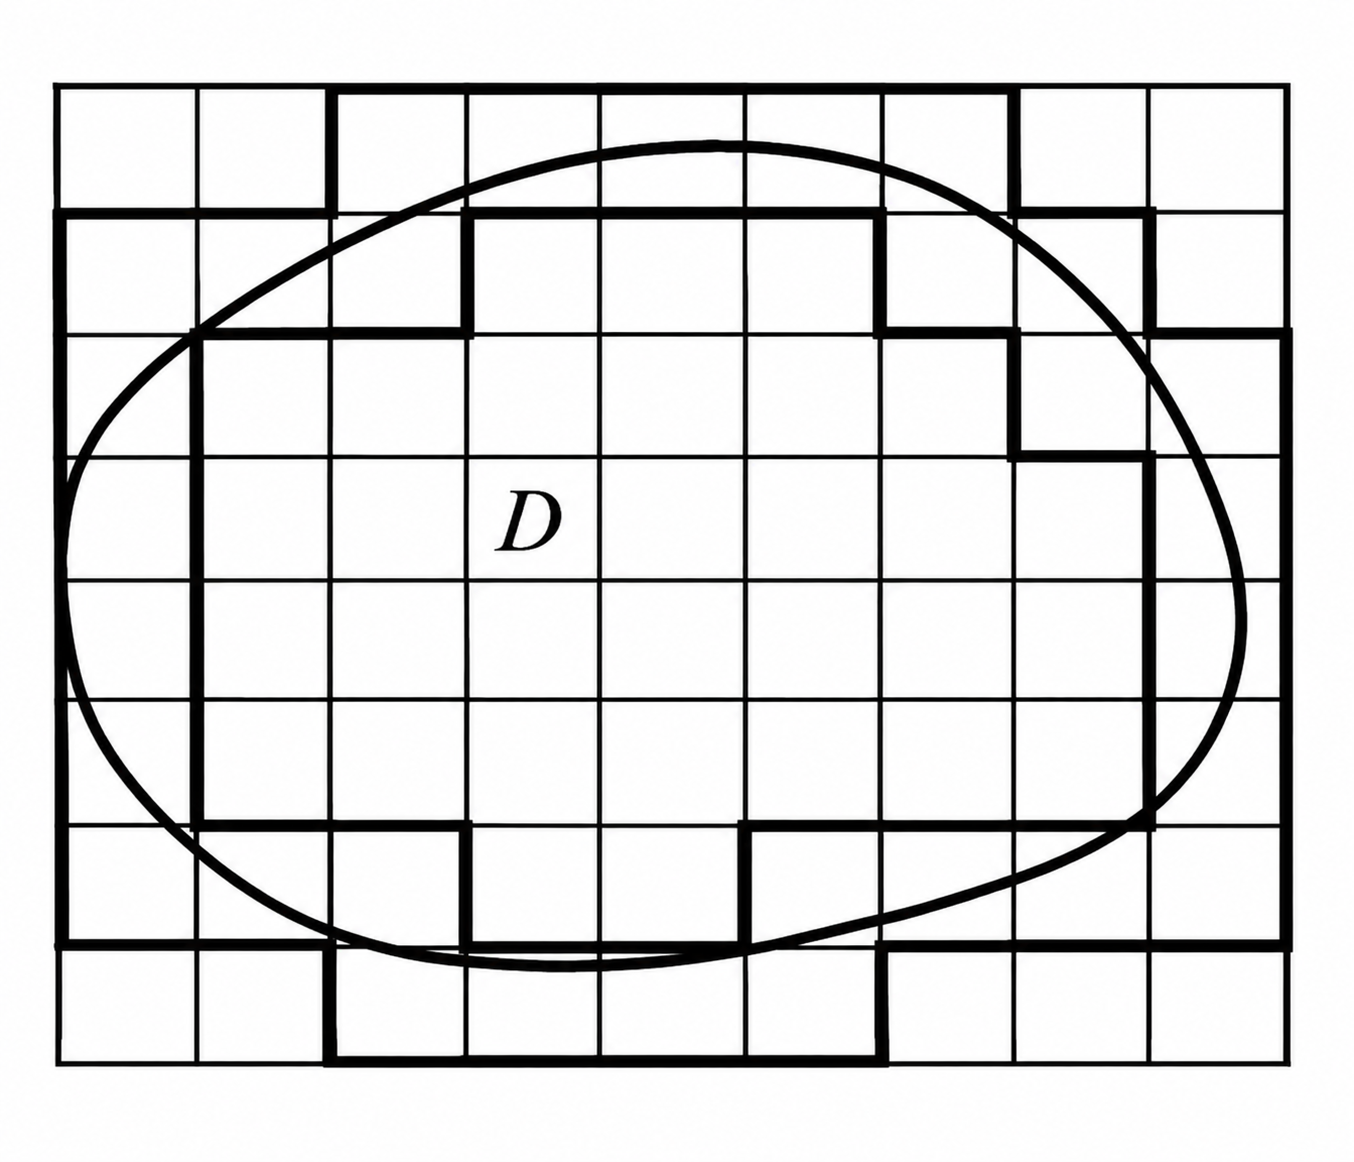
\includegraphics[width=0.29\textwidth]{figure/P2/fig13_1_1_source_hd.png}
\end{center}



\begin{proposition}\label{p2-area-refinement-comparison}
若在原有划分的基础上，在 $[a,b]$ 和 $[c,d]$ 中再增加有限个分点
（所得的新划分称为原来划分的加细），则 $mB$ 不增，$mA$ 不减；
且任意一种划分所得到的 $mA$ 不大于任意另一种划分所得到的 $mB$。
\end{proposition}
\begin{proof}
记划分 $P$ 所对应的两个面积和为 $mA(P)$ 与 $mB(P)$。
先只在一个坐标区间内增加一个分点，
得到加细后的划分 $P'$。此时每个被新分割线切到的原小矩形 $Q$
分为两个小矩形 $Q_1,Q_2$，且 $|Q|=|Q_1|+|Q_2|$。

若 $Q\subset D$，则 $Q_1,Q_2\subset D$，加细前后它对 $mA$
的贡献相等；若 $Q\not\subset D$，它原来对 $mA$ 的贡献为零，
加细后的贡献非负。因此 $mA(P)\le mA(P')$。
另一方面，若 $Q\cap D=\varnothing$，则 $Q_1,Q_2$ 均不与 $D$ 相交；
若 $Q\cap D\ne\varnothing$，加细后它们对 $mB$ 的贡献之和
至多为 $|Q_1|+|Q_2|=|Q|$。因此 $mB(P')\le mB(P)$。
依次增加有限个分点，就得到第一部分的结论。

现任取两个划分 $P_1,P_2$，将它们在两个坐标区间内的分点分别合并，
得到共同加细 $P^*$。由刚证明的单调性，以及同一划分下
$mA(P^*)\le mB(P^*)$，有
\[
mA(P_1)\le mA(P^*)\le mB(P^*)\le mB(P_2).
\]
所以任意一个 $mA$ 都不大于任意一个 $mB$。
\end{proof}


\begin{definition}
	$mA$ 有一个上确界 $mD_*$，
$mB$ 有一个下确界 $mD^*$，并且
\[
mD_*\le mD^*.
\]
若 $mD_*=mD^*$，则称这个值为 $D$ 的面积，记为 $mD$，
此时称 $D$ 是\textbf{可求面积的}。显然 $D$ 的面积与 $U$ 的选取无关。
\end{definition}

同样可以考虑 $D$ 的边界 $\partial D$ 的面积：
记与 $\partial D$ 的交集非空的那些小矩形的面积之和为
$mB_{\partial D}$。若 $mB_{\partial D}$ 的下确界
$mD^*_{\partial D}=0$，则称 $\partial D$ 的面积为零；
边界的面积为零等价于所围区域是可求面积的区域。
对任意给定的 $\varepsilon>0$，通过取足够细的划分，
可使得
\[
mB-mA=mB_{\partial D}<\varepsilon.
\]
那么就有以下的判据：
\begin{proposition}(Jordan 可求面积判据)
有界点集 $D$ 是可求面积的充分必要条件是它的边界
$\partial D$ 的面积为 $0$。
\end{proposition}

因此，零边界围成的区域是可求面积的。

面积具有可加性：如果有界点集 $D$ 由点集 $D_1$ 和 $D_2$ 组成，
$D_1$ 和 $D_2$ 可求面积，且 $D_1\cap D_2=\varnothing$，
那么 $D$ 可求面积，并满足
\[
mD=mD_1+mD_2.
\]

\begin{example}
设 $y=f(x)$（$a\le x\le b$）为非负连续函数，
它与直线 $x=a$、$x=b$ 和 $y=0$ 所围成的区域
\[
D=\{(x,y):a\le x\le b,\ 0\le y\le f(x)\}
\]
是可求面积的。

\begin{center}
% 图 13.1.2：曲线 y=f(x) 下的曲边梯形。
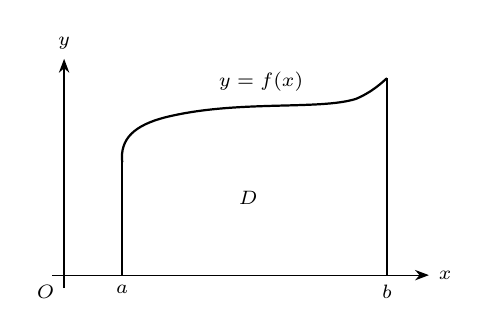
\begin{tikzpicture}[x=0.82cm,y=0.82cm,>=Stealth,baseline=(current bounding box.center)]
  \draw[->,line width=0.45pt] (-0.18,0) -- (5.65,0) node[right,font=\scriptsize] {$x$};
  \draw[->,line width=0.45pt] (0,-0.2) -- (0,3.35) node[above,font=\scriptsize] {$y$};
  \node[below left,font=\scriptsize] at (0,0) {$O$};
  \draw[line width=0.65pt] (0.9,0) -- (0.9,1.75);
  \draw[line width=0.65pt] (5.0,0) -- (5.0,3.05);
  \draw[line width=0.8pt]
    (0.9,1.75) .. controls (0.86,2.12) and (1.1,2.32) .. (1.55,2.44)
    .. controls (2.65,2.72) and (3.95,2.55) .. (4.52,2.73)
    .. controls (4.78,2.84) and (4.93,2.99) .. (5.0,3.05);
  \node[above,font=\scriptsize] at (3.05,2.69) {$y=f(x)$};
  \node[font=\scriptsize] at (2.85,1.2) {$D$};
  \node[below,font=\scriptsize] at (0.9,0) {$a$};
  \node[below,font=\scriptsize] at (5.0,0) {$b$};
\end{tikzpicture}

\end{center}

\begin{proof}
由于 $f$ 在 $[a,b]$ 上连续，那么在 $[a,b]$ 上可积。
记 $m=\min\limits_{x\in[a,b]}f(x)$，
$M=\max\limits_{x\in[a,b]}f(x)$。
若 $M=0$，则 $f\equiv0$，此时 $D=[a,b]\times\{0\}$
可用面积任意小的矩形覆盖，故面积为零，结论成立。
以下设 $M>0$。
在 $[a,b]$ 上插入分点
$a=x_0<x_1<\cdots<x_n=b$，
将 $[a,b]$ 等分，记 $h_n=(b-a)/n$；
那么矩形 $U=[a,b]\times[0,M]$ 就包含了区域 $D$。
按一元积分的 Darboux 和，令 $m_i,M_i$ 分别为
$f(x)$ 在 $[x_{i-1},x_i]$ 上的最小值与最大值。
在 $[0,M]$ 上插入分点
$m_i,M_i$（$i=1,\ldots,n$），合并重复分点后，
就得到 $U$ 的一个划分 $P_n$。
容易看出，包含于 $D$ 内的那些小矩形的面积之和为
\[
mA(P_n)=\sum_{i=1}^n m_i h_n.
\]

记 $\omega_n=\max\limits_{1\le i\le n}(M_i-m_i)$。
由 $f$ 在 $[a,b]$ 上的一致连续性，$\omega_n\to0$。
又因 $f([a,b])=[m,M]$，在 $[m,M]$ 中任意两个相邻的
$y$ 向分点 $s<t$ 都满足 $t-s\le\omega_n$。
事实上，任取 $z\in(s,t)$，存在 $x\in[a,b]$ 使 $f(x)=z$。
若 $x\in[x_{k-1},x_k]$，则 $m_k\le z\le M_k$；
由于 $m_k,M_k$ 都是分点，且 $(s,t)$ 内没有分点，
故 $m_k\le s<t\le M_k$，从而 $t-s\le M_k-m_k\le\omega_n$。

在第 $i$ 个竖条中，上边缘的纵坐标不超过 $M_i$ 的小矩形均与 $D$ 相交。
若 $M_i<M$，紧邻 $M_i$ 上方的小矩形也因在边界上与 $D$ 相交而被计入
$mB(P_n)$，但其高度至多为 $\omega_n$；
其余位于 $M_i$ 上方的小矩形不与 $D$ 相交。
因此应有估计
\[
\sum_{i=1}^n M_i h_n
\le mB(P_n)
\le\sum_{i=1}^n M_i h_n+(b-a)\omega_n.
\]
于是
\[
\sum_{i=1}^n m_i h_n
\le mD_*\le mD^*
\le\sum_{i=1}^n M_i h_n+(b-a)\omega_n.
\]
令 $n\to\infty$，由 $f$ 在 $[a,b]$ 上的可积性及极限的夹逼性得
\[
mD_*=mD^*=\int_a^b f(x)\,\dd x.
\]
因此 $D$ 是可求面积的，且面积为
$\displaystyle\int_a^b f(x)\,\dd x$。

这里证明面积存在，只需使 $mB(P_n)-mA(P_n)\to0$，
不要求划分 $P_n$ 的模长趋于零。
当 $m>0$ 时，底部区间 $[0,m]$ 无须再等分，
因为对应的小矩形完全包含于 $D$，对 $mA(P_n)$ 与 $mB(P_n)$ 的贡献相同。
\end{proof}

\textbf{注记：}按前面的定义，小矩形只要与 $D$ 的交集非空，其整个面积就计入 $mB$。
因此，仅在边界上与 $D$ 相交的闭矩形也会被计入，一般不能直接写成
$mB=\sum\limits_i M_i\Delta x_i$。
例如，取 $f(x)=x$（$0\le x\le1$），两条坐标轴上都取分点 $0,\frac12,1$，
则左上角的小矩形仅在点 $(\dfrac12,\dfrac12)$ 处与 $D$ 相交，但其面积仍被计入。
此时 $mB=1$，而 Darboux 上和为 $\dfrac34$。
\end{example}

在上述例中，记曲线 $y=f(x)$（$a\le x\le b$）为 $L$。
覆盖 $L$ 的那些小矩形
$[x_{i-1},x_i]\times[m_i,M_i]$ 的面积之和为
\[
\sum_{i=1}^n(M_i-m_i)(x_i-x_{i-1}).
\]
当 $n\to\infty$ 时，它的极限是零(由一致连续性证得)，所以曲线的面积为零。
可以用同样方法进一步证明：

平面上一条光滑曲线的面积为零。
因此，若一个有界区域的边界是分段光滑曲线，
那么它是可求面积的。

注意，并不是所有开平面点集都是可求面积的。
例如平面点集
\[
S=\{(x,y):0\le x\le1,\ 0\le y\le D(x)\},
\qquad
D(x)=
\begin{cases}
1,&x\text{ 为有理数},\\
0,&x\text{ 为无理数},
\end{cases}
\]
其中 $D(x)$ 是 Dirichlet 函数。
$S$ 的边界为 $[0,1]\times[0,1]$，它的面积为 $1$，
这说明 $S$ 不是可求面积的。

\subsection*{二重积分的概念}

考察一个曲顶柱体：它的底是 $xy$ 平面上的具有零边界的
有界闭区域 $D$，顶是非负连续函数 $z=f(x,y)$，
$(x,y)\in D$ 所确定的曲面，侧面是以 $D$ 的边界曲线为准线、
母线平行于 $z$ 轴的柱面。

\begin{center}
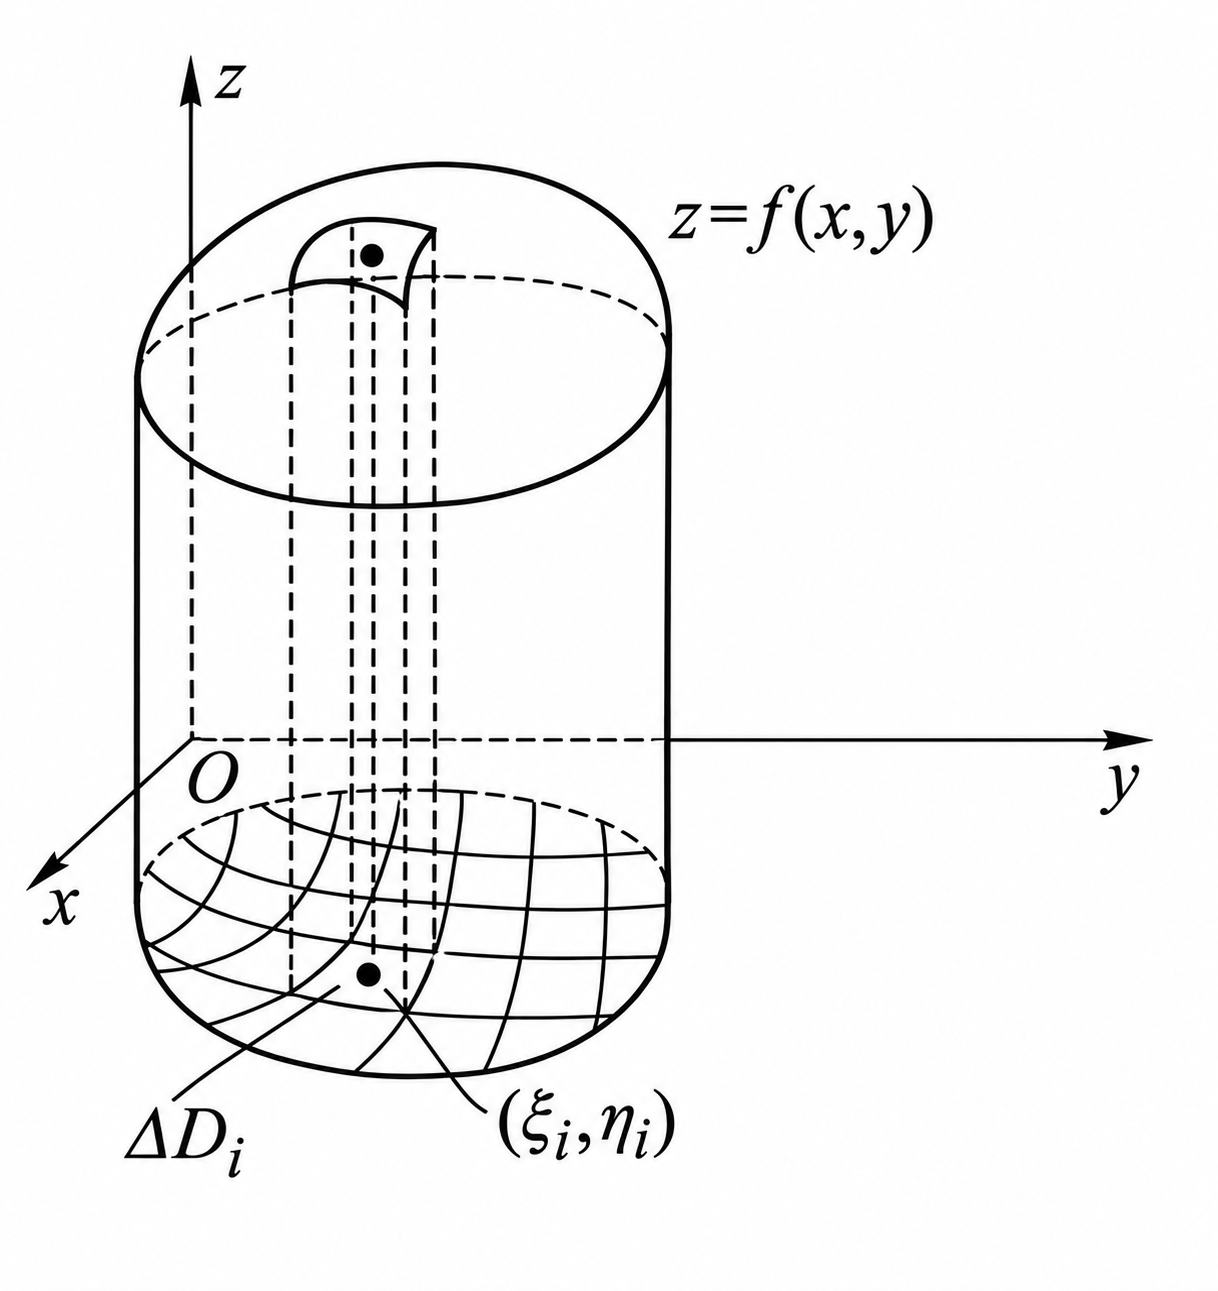
\includegraphics[width=0.34\textwidth]{figure/P2/fig13_1_3_source_hd.png}
\end{center}

为了求出它的体积 $V$，先用一些面积为零的曲线段组成的曲线网
将区域 $D$ 分成 $n$ 个小区域
$\Delta D_1,\Delta D_2,\ldots,\Delta D_n$。
由前面的讨论，每个 $\Delta D_i$ 都是可求面积的
（$i=1,2,\ldots,n$）。
再分别以这些小区域的边界为准线，作母线平行于
$z$ 轴的柱面，这些柱面将原曲顶柱体分成 $n$ 个细的小曲顶柱体。
在每个 $\Delta D_i$ 上任取一点 $(\xi_i,\eta_i)$，
那么以 $\Delta D_i$ 为底的小曲顶柱体的体积近似地等于
\[
f(\xi_i,\eta_i)\Delta\sigma_i,
\]
这里 $\Delta\sigma_i$ 表示 $\Delta D_i$ 的面积。
于是，原曲顶柱体的体积近似地等于
\[
\sum_{i=1}^n f(\xi_i,\eta_i)\Delta\sigma_i.
\]
当所有小区域 $\Delta D_i$ 的最大直径（记为 $\lambda = \max \limits_{1\leqslant k \leqslant  n}\operatorname{diam}\Delta_k$）
趋于零时，这个近似值趋于原曲顶柱体的体积，即
\[
V=\lim_{\lambda\to0}
\sum_{i=1}^n f(\xi_i,\eta_i)\Delta\sigma_i.
\]
这就是二重积分的概念。
以下讨论积分存在性时，总假定区域的边界以及
用来分割区域的曲线段的面积为零，
这就保证了所涉及的一切区域的面积都存在。

\begin{definition}[二重积分]
设 $D$ 为 $\R^2$ 上的\textbf{零边界闭区域}，函数 $z=f(x,y)$ 在 $D$ 上有界。
将 $D$ 用曲线网分成 $n$ 个小区域
$\Delta D_1,\Delta D_2,\ldots,\Delta D_n$
（它称为 $D$ 的一个划分），并记所有小区域
$\Delta D_i$ 的最大直径为
\[
\lambda=\max_{1\le i\le n}|\operatorname{diam}\Delta D_i|.
\]
在每个 $\Delta D_i$ 上任取一点 $(\xi_i,\eta_i)$，
记 $\Delta\sigma_i$ 为 $\Delta D_i$ 的面积。
若 $\lambda$ 趋于零时，和式
\[
\sum_{i=1}^n f(\xi_i,\eta_i)\Delta\sigma_i
\]
的极限存在，且与区域的分法和点
$(\xi_i,\eta_i)$ 的取法无关，
则称 $f(x,y)$ 在 $D$ 上可积，并称此极限为
$f(x,y)$ 在 $D$ 上的\textbf{二重积分}，记为
\[
\iint_D f(x,y)\,\dd\sigma
=\lim_{\lambda\to0}
\sum_{i=1}^n f(\xi_i,\eta_i)\Delta\sigma_i.
\]
$f(x,y)$ 称为被积函数，$D$ 称为积分区域，
$x$ 和 $y$ 称为积分变量，$\dd\sigma$ 称为面积元素，
$\displaystyle\iint_D f(x,y)\,\dd\sigma$ 也称为积分值。
\end{definition}

用 $\varepsilon$-$\delta$ 语言，上述定义是：
对任意 $\varepsilon>0$，存在 $\delta>0$，
使对任意划分 $P$ 及任意选点 $ \vect q_i\in\Delta D_i$，
只要 $\lambda(P)<\delta$，就有
\[
\left|\sum_i f(\vect q_i)\Delta\sigma_i-I\right|<\varepsilon.
\]
这里 $I$ 为同一个常数，$\delta$ 不依赖于划分及选点。

前面提到的曲顶柱体的体积即为
\[
V=\iint_D f(x,y)\,\dd\sigma.
\]

与一元的情况类似，下面用 Darboux 和讨论二重积分的可积性。
以下始终设 $D$ 为有界零边界闭区域，$f$ 在 $D$ 上有界，
记 $\sigma=mD$。
划分 $P=\{\Delta D_1,\ldots,\Delta D_n\}$ 中各小区域取为闭的小块，
其内部互不相交，公共边界的面积为零，因而
\[
\sum_{i=1}^n\Delta\sigma_i=\sigma,
\qquad
\lambda(P)=\max_{1\le i\le n}\operatorname{diam}\Delta D_i.
\]
非空的零面积小块也可保留在划分中，它们对各和式的贡献为零。
两划分合并曲线网所得的共同加细，可用原有小块的非空交集表示；
若交集分成多个小区域，对它们的贡献求和即可。
这些子块的边界仍包含于原有零面积边界的并集中。
用矩形网与 $D$ 相交，可得到模长任意小的划分。

设
\[
M_i=\sup_{\Delta D_i}f,\qquad
m_i=\inf_{\Delta D_i}f,\qquad
\omega_i=M_i-m_i,
\]
定义 Darboux 大和、小和分别为
\[
S(P)=\sum_{i=1}^n M_i\Delta\sigma_i,\qquad
s(P)=\sum_{i=1}^n m_i\Delta\sigma_i.
\]
其中 $\omega_i$ 称为 $f$ 在 $\Delta D_i$ 上的振幅。
在各小块中任取点 $\vect q_i=(\xi_i,\eta_i)$，
相应的 Riemann 和记为
\[
J(P;\vect q)=\sum_{i=1}^n f(\vect q_i)\Delta\sigma_i,
\qquad
s(P)\le J(P;\vect q)\le S(P).
\]

沿用命题 \ref{p2-area-refinement-comparison} 中逐块估计和共同加细的论证，
可得 Darboux 和的相应性质：
加细后，各子块的上确界不大于原小块的上确界，
下确界不小于原小块的下确界；再由面积的可加性，
若 $P'$ 是 $P$ 的加细，就有
\[
s(P)\le s(P')\le S(P')\le S(P).
\]
任取两个划分 $P_1,P_2$，将它们合并为共同加细 $P^*$，则
\[
s(P_1)\le s(P^*)\le S(P^*)\le S(P_2).
\]
所以任何一个 Darboux 小和都不大于任何一个 Darboux 大和。
记 $m=\inf_D f$、$M=\sup_D f$，还有
\[
m\sigma\le s(P_1)\le S(P_2)\le M\sigma.
\]
因此，由实数的确界存在定理，所有 Darboux 小和的上确界
与所有 Darboux 大和的下确界都存在。
分别称
\[
I_*=\sup_P s(P),\qquad I^*=\inf_P S(P)
\]
为 $f$ 在 $D$ 上的\textbf{下积分}和\textbf{上积分}。
这里的确界取遍本节定义所允许的全部划分 $P$，
不涉及小块内选点的取法，也不要求预先知道 $f$ 可积。
上、下积分可能不相等，但对任意划分 $P$ 都有
\[
m\sigma\le s(P)\le I_*\le I^*\le S(P)\le M\sigma.
\]

% 对应第一部分命题 8.3.8。
\begin{proposition}[二重积分的 Darboux 定理]\label{p2-darboux-limit}
当划分的模长 $\lambda(P)\to0$ 时，
\[
S(P)\to I^*,\qquad s(P)\to I_*.
\]
即对任意 $\varepsilon>0$，存在 $\delta>0$，
使得对任意划分 $P$，只要 $\lambda(P)<\delta$，就有
\[
0\le S(P)-I^*<\varepsilon,\qquad
0\le I_*-s(P)<\varepsilon.
\]
\end{proposition}
\begin{proof}
先说明任意充分细的划分与一个固定划分合并时，和式的变化可以任意小。
固定 $P_0=\{E_1,\ldots,E_r\}$，记
\[
\Gamma=\bigcup_{j=1}^r\partial E_j.
\]
由于区域边界和分割曲线的面积为零，$\Gamma$ 是面积为零的紧集。
任给 $\alpha>0$，可用有限个开矩形覆盖 $\Gamma$，
使其面积之和小于 $\alpha$；记这些开矩形的并为 $G$。
由 $\Gamma$ 的紧性，存在 $\rho>0$，使
\[
\Gamma_\rho=\{z:\operatorname{d}(z,\Gamma)<\rho\}\subset G.
\]

设 $P^*$ 为 $P,P_0$ 的共同加细。
把 $P$ 中不包含于任何一个 $E_j$ 的小块称为受影响的小块。
若 $\lambda(P)<\rho/2$，则每个受影响的小块都包含于 $G$。
事实上，任取其中一点 $p$，选取含 $p$ 的 $E_j$；
由于该小块不包含于 $E_j$，其中还存在 $q\notin E_j$。
线段 $pq$ 必经过 $\partial E_j$ 上某点 $z$，
于是对该小块中任意点 $w$，
\[
|w-z|\le |w-p|+|p-z|
\le 2\lambda(P)<\rho.
\]
所以该小块包含于 $\Gamma_\rho$。
各小块只在零面积边界上重叠，故受影响小块的面积之和 $A(P)$ 满足
\[
A(P)\le mG<\alpha.
\]

记 $K=M-m$。未受影响的小块在共同加细前后贡献不变，
受影响小块的上、下和变化分别不超过 $K$ 乘以该小块的面积，故
\[
\begin{aligned}
0&\le S(P)-S(P^*)\le K A(P),\\
0&\le s(P^*)-s(P)\le K A(P).
\end{aligned}
\]
因此对固定的 $P_0$，上述两种变化都随 $\lambda(P)\to0$ 而趋于零。

现证明 $S(P)\to I^*$。
任给 $\varepsilon>0$，由下确界的定义，可取固定划分 $P_0$，使
\[
0\le S(P_0)-I^*<\frac{\varepsilon}{2}.
\]
在前面的估计中取 $\alpha=\varepsilon/[2(K+1)]$，
并取相应的 $\delta=\rho/2$。
当 $\lambda(P)<\delta$ 时，
\[
\begin{aligned}
0\le S(P)-I^*
&=S(P)-S(P^*)+S(P^*)-I^*\\
&\le K A(P)+S(P_0)-I^*
<\varepsilon.
\end{aligned}
\]
同理，由上确界的定义，先取 $s(P_0)>I_*-\varepsilon/2$，
再用 $s(P^*)\ge s(P_0)$，即可得到 $0\le I_*-s(P)<\varepsilon$。
\end{proof}

% 对应第一部分命题 8.3.9。
\begin{proposition}[上下积分相等判据]\label{p2-integrability-upper-lower}
$f$ 在 $D$ 上可积的充分必要条件是 $I_*=I^*$。
此时
\[
\iint_D f(x,y)\,\dd\sigma=I_*=I^*.
\]
\end{proposition}
\begin{proof}
必要性：设 $f$ 可积，积分值为 $I$。
任给 $\varepsilon>0$，由积分定义，存在 $\delta>0$，
使得当 $\lambda(P)<\delta$ 时，对任意选点 $\vect q_i$ 都有
\[
|J(P;\vect q)-I|<\varepsilon.
\]
对这样的划分，由上确界的定义，可以逐块选取 $\vect q_i^+$，使
\[
M_i-\frac{\varepsilon}{\sigma+1}<f(\vect q_i^+)\le M_i.
\]
于是
\[
0\le S(P)-J(P;\vect q^+)\le
\frac{\varepsilon\sigma}{\sigma+1}<\varepsilon,
\]
故 $|S(P)-I|<2\varepsilon$。
同理，逐块选取逼近下确界的点，得到 $|s(P)-I|<2\varepsilon$。
结合命题 \ref{p2-darboux-limit}，可知 $I^*=I_*=I$。
这里不要求上、下确界能在小块中取到。

充分性：设 $I_*=I^*=I$。
由命题 \ref{p2-darboux-limit}，当 $\lambda(P)\to0$ 时，
$s(P),S(P)$ 都趋于 $I$。
而任意选点所得的 Riemann 和都满足
\[
s(P)\le J(P;q)\le S(P).
\]
由夹逼性，其极限为 $I$，且与划分及选点无关，即 $f$ 可积。
\end{proof}

% 对应第一部分定理 8.3.10。
\begin{theorem}(二重积分可积的第一充要条件)\label{p2-integrability-first}
$f$ 在 $D$ 上可积的充分必要条件是
\[
\lim_{\lambda(P)\to0}\bigl(S(P)-s(P)\bigr)
=\lim_{\lambda(P)\to0}\sum_{i=1}^n\omega_i\Delta\sigma_i=0.
\]
即对任意 $\varepsilon>0$，存在 $\delta>0$，
使得对任意划分 $P$，只要 $\lambda(P)<\delta$，就有
\[
\sum_{i=1}^n\omega_i\Delta\sigma_i<\varepsilon.
\]
此时
\[
\lim_{\lambda(P)\to0}s(P)
=\lim_{\lambda(P)\to0}S(P)
=\iint_D f(x,y)\,\dd\sigma.
\]
\end{theorem}
\begin{proof}
由命题 \ref{p2-darboux-limit}，
\[
\lim_{\lambda(P)\to0}\bigl(S(P)-s(P)\bigr)=I^*-I_*.
\]
结合命题 \ref{p2-integrability-upper-lower} 及
$S(P)-s(P)=\sum_i\omega_i\Delta\sigma_i$，即得结论。
\end{proof}

% 对应第一部分定理 8.3.11。
\begin{theorem}(二重积分可积的第二充要条件)\label{p2-integrability-second}
$f$ 在 $D$ 上可积的充分必要条件是：
对任意 $\varepsilon>0$，存在一个划分 $P$，使得
\[
S(P)-s(P)=\sum_{i=1}^n\omega_i\Delta\sigma_i<\varepsilon.
\]
这里所取划分不必预先满足某个模长限制。
\end{theorem}
\begin{proof}
必要性：由定理 \ref{p2-integrability-first}，
取一个模长充分小的划分即可。

充分性：由 $s(P)\le I_*\le I^*\le S(P)$，
对上述划分有
\[
0\le I^*-I_*\le S(P)-s(P)<\varepsilon.
\]
由于 $\varepsilon>0$ 任意，必有 $I^*=I_*$。
由命题 \ref{p2-integrability-upper-lower}，$f$ 在 $D$ 上可积。
\end{proof}

% 对应第一部分定理 8.3.12。
\begin{theorem}(二重积分可积的第三充要条件)\label{p2-integrability-third}
$f$ 在 $D$ 上可积，当且仅当：
对任意 $\varepsilon>0$、$\eta>0$，存在划分 $P$，
使振幅不小于 $\eta$ 的小块的面积之和小于 $\varepsilon$，即
\[
\sum_{\omega_i\ge\eta}\Delta\sigma_i<\varepsilon.
\]
\end{theorem}
\begin{proof}
必要性：设 $f$ 可积。
任给 $\varepsilon>0$、$\eta>0$，由定理 \ref{p2-integrability-second}，
存在划分 $P$，使 $\sum_i\omega_i\Delta\sigma_i<\varepsilon\eta$。
于是
\[
\eta\sum_{\omega_i\ge\eta}\Delta\sigma_i
\le\sum_{\omega_i\ge\eta}\omega_i\Delta\sigma_i
\le\sum_i\omega_i\Delta\sigma_i<\varepsilon\eta.
\]
除以 $\eta>0$，即得所需结论。

充分性：记 $K=M-m$。
任给 $\varepsilon>0$，取
\[
\varepsilon'=\frac{\varepsilon}{2(K+1)},\qquad
\eta=\frac{\varepsilon}{2(\sigma+1)}.
\]
由条件，存在划分 $P$，使
$\sum_{\omega_i\ge\eta}\Delta\sigma_i<\varepsilon'$。
将小块分为 $\omega_i\ge\eta$ 与 $\omega_i<\eta$ 两类，有
\[
\begin{aligned}
\sum_i\omega_i\Delta\sigma_i
&=\sum_{\omega_i\ge\eta}\omega_i\Delta\sigma_i
+\sum_{\omega_i<\eta}\omega_i\Delta\sigma_i\\
&\le K\sum_{\omega_i\ge\eta}\Delta\sigma_i
+\eta\sum_{\omega_i<\eta}\Delta\sigma_i\\
&\le K\varepsilon'+\eta\sigma
<\varepsilon.
\end{aligned}
\]
由定理 \ref{p2-integrability-second}，$f$ 在 $D$ 上可积。
分母中加 $1$，也使 $K=0$ 或 $\sigma=0$ 的情形一并成立。
\end{proof}

\begin{proposition}\label{p2-continuous-integrability}
若 $f(x,y)$ 在零边界闭区域 $D$ 上连续，
那么它在 $D$ 上可积。
\end{proposition}
\begin{proof}
记 $\sigma$ 为 $D$ 的面积。若 $\sigma=0$，
则结论直接成立。若 $\sigma>0$，
由于 $f(x,y)$ 在紧集 $D$ 上连续，
所以它在 $D$ 上一致连续。
于是对任意 $\varepsilon>0$，
存在 $\delta>0$，使得当
\[
\sqrt{(x_1-x_2)^2+(y_1-y_2)^2}<\delta
\]
时，成立
\[
|f(x_1,y_1)-f(x_2,y_2)|<\frac{\varepsilon}{2\sigma}.
\]
因此对 $D$ 的任一划分
$\Delta D_1,\Delta D_2,\ldots,\Delta D_n$，
当所有 $\Delta D_i$ 的最大直径 $\lambda<\delta$ 时，
$f(x,y)$ 在每个 $\Delta D_i$ 上的振幅
$\omega_i$ 就不大于 $\varepsilon/(2\sigma)$。
这就成立
\[
\sum_{i=1}^n\omega_i\Delta\sigma_i
\le\frac{\varepsilon}{2\sigma}
\sum_{i=1}^n\Delta\sigma_i
=\frac{\varepsilon}{2\sigma}\,\sigma
=\frac{\varepsilon}{2}<\varepsilon.
\]
所以
$\lim\limits_{\lambda\to0}\sum_{i=1}^n\omega_i\Delta\sigma_i=0$，
由定理 \ref{p2-integrability-first}，$f(x,y)$ 在 $D$ 上可积。
\end{proof}

\begin{corollary}[除有限条零面积曲线外连续的函数可积]\label{p2-curve-discontinuity-integrability}
设 $D$ 为有界零边界闭区域，$f(x,y)$ 在 $D$ 上有界。
若 $f$ 的不连续点都包含在有限条面积为零的连续曲线
$\Gamma_1,\ldots,\Gamma_r$ 上，则 $f$ 在 $D$ 上可求二重积分。
这里每条曲线均为闭有限区间的连续像，连续性均指相对于 $D$ 的连续性。
特别地，若 $f$ 除有限条分段光滑曲线外处处连续，则 $f$ 在 $D$ 上可积。
\end{corollary}
\begin{proof}
记 $\sigma=mD$，取 $B\ge0$ 使 $|f(x,y)|\le B$。
若 $\sigma=0$，则所有 Riemann 和均为零，结论成立。
若没有异常曲线，则由定理 \ref{p2-continuous-integrability}，结论成立。
以下设 $\sigma>0$，且
\[
E=\bigcup_{j=1}^r\Gamma_j
\]
非空。$E$ 是面积为零的紧集。
任给 $\varepsilon>0$，用有限个开矩形覆盖 $E$，
使这些矩形的面积之和小于 $\varepsilon/[4(B+1)]$。
记其并为 $G$，则
\[
mG<\frac{\varepsilon}{4(B+1)}.
\]
由 $E$ 的紧性，存在 $\rho>0$，使
\[
E_\rho=\{z:\operatorname{d}(z,E)<\rho\}\subset G.
\]
令 $H=E_{\rho/2}$、$K=D\setminus H$。
由于 $H$ 为开集，$K$ 为紧集，且 $K\cap E=\varnothing$，
所以 $f$ 在 $K$ 上连续，从而一致连续。
若 $K\ne\varnothing$，可取 $\delta_1>0$，使对任意 $p,q\in K$，
\[
|p-q|<\delta_1
\quad\Longrightarrow\quad
|f(p)-f(q)|<\frac{\varepsilon}{2(\sigma+1)}.
\]
若 $K=\varnothing$，则下述第二类小块不存在，此时任取 $\delta_1>0$。

取 $\delta=\min\{\rho/2,\delta_1\}$。
对任意满足 $\lambda(P)<\delta$ 的划分 $P$，
将小块分成两类。
第一类为与 $H$ 相交的小块；若 $p\in\Delta D_i\cap H$，
则对任意 $q\in\Delta D_i$，
\[
\operatorname{d}(q,E)
\le |q-p|+\operatorname{dist}(p,E)
<\delta+\frac{\rho}{2}\le\rho.
\]
所以这类小块都包含于 $G$，其面积之和不超过 $mG$。
又因 $\omega_i\le2B$，这类小块的贡献满足
\[
\sum_{\Delta D_i\cap H\ne\varnothing}\omega_i\Delta\sigma_i
\le2B\,mG<\frac{\varepsilon}{2}.
\]
第二类为不与 $H$ 相交的小块，它们都包含于 $K$。
由一致连续性，每个小块的振幅不大于 $\varepsilon/[2(\sigma+1)]$，
故这类小块的贡献满足
\[
\sum_{\Delta D_i\cap H=\varnothing}\omega_i\Delta\sigma_i
\le\frac{\varepsilon}{2(\sigma+1)}
\sum_{\Delta D_i\cap H=\varnothing}\Delta\sigma_i
\le\frac{\varepsilon\sigma}{2(\sigma+1)}
<\frac{\varepsilon}{2}.
 \]
合并两类估计，得到
\[
\sum_i\omega_i\Delta\sigma_i<\varepsilon.
\]
由定理 \ref{p2-integrability-first}，$f$ 在 $D$ 上可积。
\end{proof}

\textbf{注记：}异常曲线上的函数值可以任意取，只需整个函数仍有界。
推论中要求异常曲线的面积为零；仅有曲线的连续性不能代替这一条件。
连续函数的图像以及分段光滑曲线都满足这一零面积条件。

\subsection*{$n$ 重积分}

同 $\R^2$ 中定义面积一样，可以在 $\R^n$（$n\ge3$）中引入体积的概念。
若定义 $\R^n$ 中的 $n$ 维闭矩形
\[
[a_1,b_1]\times[a_2,b_2]\times\cdots\times[a_n,b_n]
\]
的体积为
$(b_1-a_1)(b_2-a_2)\cdots(b_n-a_n)$，
那么就可以将 $\R^2$ 上定义面积的叙述
完全平移到 $\R^n$（$n\ge3$）上来定义体积。
同样称边界体积为零的有界区域为零边界区域；
而且可以证明，光滑曲面的体积为零。
这里就不一一详述了。
设 $\Omega$ 是 $\R^n$（$n\ge3$）上的有界区域，
其边界是一张或数张无重点的封闭曲面
（本章总是如此假定），
那么同样可得：有界点集 $\Omega$ 是可求体积的
充分必要条件为其边界的体积为零，
即 $\Omega$ 为零边界区域。

同 $\R^2$ 中的原理一样，引入 $n$ 重积分的概念。
\begin{definition}[$n$ 重积分]
设 $\Omega$ 为 $\R^n$ 上的零边界闭区域，
函数 $u=f(x)$ 在 $\Omega$ 上有界。
将 $\Omega$ 用曲面网分成 $n$ 个小区域
$\Delta\Omega_1,\Delta\Omega_2,\ldots,\Delta\Omega_n$
（称为 $\Omega$ 的一个划分），
记 $\Delta V_i$ 为 $\Delta\Omega_i$ 的体积，
并记所有小区域 $\Delta\Omega_i$ 的最大直径为 $\lambda$。
在每个 $\Delta\Omega_i$ 上任取一点 $x_i$，
若 $\lambda$ 趋于零时，和式
\[
\sum_{i=1}^n f(x_i)\Delta V_i
\]
的极限存在，且与区域的分法和点 $x_i$ 的取法无关，
则称 $f(x)$ 在 $\Omega$ 上可积，
并称此极限为 $f(x)$ 在有界闭区域 $\Omega$ 上的
$n$ 重积分，记为
\[
\int_\Omega f\,\dd V
=\lim_{\lambda\to0}\sum_{i=1}^n f(x_i)\Delta V_i.
\]
$f(x)$ 称为被积函数，$\Omega$ 称为积分区域，
$x$ 称为积分变量，$\dd V$ 称为体积元素，
$\displaystyle \int_\Omega f\,\dd V$ 也称为积分值。
\end{definition}

类似于二维情形可知，若 $f(x)$ 在零边界闭区域
$\Omega$ 上连续，那么它在 $\Omega$ 上可积。
注意到 $n=2$ 与 $n>2$ 的重积分定义并没有本质的区别，
今后我们经常把它们一起讨论。
为明确起见，通常采用如下记法：
\[
\begin{aligned}
&\text{在 }\R^2\text{ 中：}&
&\iint_D f(x,y)\,\dd x\,\dd y;\\
&\text{在 }\R^3\text{ 中：}&
&\iiint_\Omega f(x,y,z)\,\dd x\,\dd y\,\dd z
\quad\text{或}\quad
\iiint_\Omega f(x,y,z)\,\dd V;\\
&\text{在 }\R^n\text{ 中：}&
&\int_\Omega f(x_1,\ldots,x_n)
\,\dd x_1\cdots\dd x_n
\quad\text{或}\quad
\idotsint_\Omega f(x_1,\ldots,x_n)
\,\dd x_1\cdots\dd x_n.
\end{aligned}
\]

\begin{example}
设 $\Omega\subset\R^3$ 为具有分片光滑表面的物体，
$f(x,y,z)$ 是 $\Omega$ 在 $(x,y,z)$ 处的密度。
将 $\Omega$ 用分片光滑曲面分成充分小的块
$\Delta\Omega_1,\Delta\Omega_2,\ldots,\Delta\Omega_n$，
那么 $f(\xi_i,\eta_i,\zeta_i)\Delta V_i$
就近似地为 $\Delta\Omega_i$ 的质量；
这里 $\Delta V_i$ 为 $\Delta\Omega_i$ 的体积，
$(\xi_i,\eta_i,\zeta_i)$ 为 $\Delta\Omega_i$ 任一点。
于是
\[
\sum_{i=1}^n f(\xi_i,\eta_i,\zeta_i)\Delta V_i
\]
就近似地表示 $\Omega$ 的质量。
以 $\lambda$ 表示所有 $\Delta\Omega_i$ 的最大直径，
则 $\Omega$ 的质量为
\[
M=\lim_{\lambda\to0}
\sum_{i=1}^n f(\xi_i,\eta_i,\zeta_i)\Delta V_i
=\iiint_\Omega f(x,y,z)\,\dd x\,\dd y\,\dd z.
\]

现在来计算此物体的质心
$(\bar x,\bar y,\bar z)$。
如果空间上有 $n$ 个质点，它们的质量分别为
$m_1,m_2,\ldots,m_n$，
且相应地位于点
$(x_1,y_1,z_1),\ldots,(x_n,y_n,z_n)$，
那么这些质点系的质心坐标为
\[
\bar x=\frac{\sum_{i=1}^n m_i x_i}{\sum_{i=1}^n m_i},
\qquad
\bar y=\frac{\sum_{i=1}^n m_i y_i}{\sum_{i=1}^n m_i},
\qquad
\bar z=\frac{\sum_{i=1}^n m_i z_i}{\sum_{i=1}^n m_i}.
\]
当 $\lambda$ 充分小时，
可将 $\Omega$ 看成质点
$f(\xi_i,\eta_i,\zeta_i)\Delta V_i$ 的系统；
其中 $(\xi_i,\eta_i,\zeta_i)$ 为
$\Delta\Omega_i$ 上任一点。
那么其质心坐标为
\[
\begin{aligned}
\bar x&\approx
\frac{\sum_{i=1}^n
\xi_i f(\xi_i,\eta_i,\zeta_i)\Delta V_i}
{\sum_{i=1}^n f(\xi_i,\eta_i,\zeta_i)\Delta V_i},\\
\bar y&\approx
\frac{\sum_{i=1}^n
\eta_i f(\xi_i,\eta_i,\zeta_i)\Delta V_i}
{\sum_{i=1}^n f(\xi_i,\eta_i,\zeta_i)\Delta V_i},\\
\bar z&\approx
\frac{\sum_{i=1}^n
\zeta_i f(\xi_i,\eta_i,\zeta_i)\Delta V_i}
{\sum_{i=1}^n f(\xi_i,\eta_i,\zeta_i)\Delta V_i}.
\end{aligned}
\]
因此当 $\lambda$ 趋于零时得到
\[
\begin{aligned}
\bar x&=
\frac{\iiint_\Omega x f(x,y,z)\,\dd x\,\dd y\,\dd z}
{\iiint_\Omega f(x,y,z)\,\dd x\,\dd y\,\dd z},\\
\bar y&=
\frac{\iiint_\Omega y f(x,y,z)\,\dd x\,\dd y\,\dd z}
{\iiint_\Omega f(x,y,z)\,\dd x\,\dd y\,\dd z},\\
\bar z&=
\frac{\iiint_\Omega z f(x,y,z)\,\dd x\,\dd y\,\dd z}
{\iiint_\Omega f(x,y,z)\,\dd x\,\dd y\,\dd z}.
\end{aligned}
\]
注意上式的分母就是 $\Omega$ 的质量。
\end{example}

% 来源：0022F7626EB44AE5E21B9ED8C4E5E753.png，先左栏后右栏。
%
% 第2节：重积分的性质与计算
% !TEX root = ../../../main.tex
% 所属：第二部分：多变量分析学 / 第3章：重积分
% 节：3.2 重积分的性质与计算
% 正文按原文件顺序保存；由 ../chapter3.tex 调用。
\section{重积分的性质与计算}

\subsection*{性质}

除非特别声明，本节所考虑的区域是 $\R^n$（$n\ge2$）中的\textbf{零边界闭区域}。

证明中记 $V$ 为 $\Omega$ 的面积或体积，
$P=\{\Delta\Omega_i\}_{i=1}^N$ 为 $\Omega$ 的划分，
$\Delta V_i$ 为各小块的面积或体积，因而 $\sum_i\Delta V_i=V$。
对有界函数 $u$，记
\[
\omega_i(u)=\sup_{\Delta\Omega_i}u-\inf_{\Delta\Omega_i}u,
\qquad
J_u(P;\xi)=\sum_i u(\vect\xi_i)\Delta V_i,
\quad \vect\xi_i\in\Delta\Omega_i.
\]
前节的 Darboux 和及振幅判据在 $n$ 维情形仍成立：
只需将小块的面积换成体积，将零面积分割边界换成零体积分割边界，
其共同加细与边界邻域估计的证明相同。
以下证明沿用第一部分第八章第四节的方法。

\begin{proposition}[线性性]\label{p2-integral-linearity}
设 $f$ 和 $g$ 都在区域 $\Omega$ 上可积，$\alpha,\beta$ 为常数，
则 $\alpha f+\beta g$ 在 $\Omega$ 上也可积，并且
\[
\int_\Omega(\alpha f+\beta g)\,\dd V
=\alpha\int_\Omega f\,\dd V+\beta\int_\Omega g\,\dd V.
\]
\end{proposition}
\begin{proof}
设 $h=\alpha f+\beta g$。由于 $f,g$ 有界，$h$ 也有界。
对同一小块中的任意两点 $\vect p,\vect q$，有
\[
|h(\vect p)-h(\vect q)|
\le|\alpha|\,|f(\vect p)-f(\vect q)|
+|\beta|\,|g(\vect p)-g(\vect q)|.
\]
取上确界，得到
\[
\omega_i(h)\le|\alpha|\omega_i(f)+|\beta|\omega_i(g).
\]
由 $f,g$ 的可积性，当 $\lambda(P)\to0$ 时，
\[
0\le\sum_i\omega_i(h)\Delta V_i
\le|\alpha|\sum_i\omega_i(f)\Delta V_i
+|\beta|\sum_i\omega_i(g)\Delta V_i\longrightarrow0.
\]
由振幅判据，$h$ 可积。
在同一划分中选取同样的点，则 Riemann 和满足
\[
J_h(P;\xi)=\alpha J_f(P;\xi)+\beta J_g(P;\xi).
\]
令 $\lambda(P)\to0$，由极限的线性性，即得所需积分等式。
\end{proof}

\begin{proposition}[区域可加性]\label{p2-integral-domain-additivity}
设区域 $\Omega$ 被分成两个内部互不相交的区域 $\Omega_1,\Omega_2$。
若 $f$ 在 $\Omega$ 上可积，则 $f$ 在 $\Omega_1,\Omega_2$ 上都可积；
反之，若 $f$ 在 $\Omega_1,\Omega_2$ 上都可积，则 $f$ 在 $\Omega$ 上也可积。
此时成立
\[
\int_\Omega f\,\dd V
=\int_{\Omega_1}f\,\dd V+\int_{\Omega_2}f\,\dd V.
\]
\end{proposition}
\begin{proof}
两个子区域也满足本节的零边界假定。
公共部分包含于 $\partial\Omega_1\cup\partial\Omega_2$ 中，故其面积或体积为零，
划分的面积或体积之和不会因公共边界重复而改变。

必要性：设 $f$ 在 $\Omega$ 上可积。
任给 $\varepsilon>0$，由第二充要条件，可取 $\Omega$ 的划分 $P$，使
\[
\sum_i\omega_i(f)\Delta V_i<\varepsilon.
\]
将 $P$ 的小块分别与 $\Omega_1,\Omega_2$ 相交，得到加细划分 $P^*$。
加细时大和不增、小和不减，故振幅和不增。
将 $P^*$ 限制在 $\Omega_j$ 上，得到 $\Omega_j$ 的划分 $P_j$，
其振幅和只是 $P^*$ 的振幅和中相应的非负部分。因此
\[
\sum_{\Delta E\in P_j}\omega_{\Delta E}(f)\,m(\Delta E)
\le\sum_{\Delta E\in P^*}\omega_{\Delta E}(f)\,m(\Delta E)
\le\sum_i\omega_i(f)\Delta V_i<\varepsilon,
\]
其中 $m(\Delta E)$ 表示小块的面积或体积。
由第二充要条件，$f$ 在 $\Omega_1,\Omega_2$ 上都可积。

充分性：设 $f$ 在 $\Omega_1,\Omega_2$ 上都可积，则它在 $\Omega$ 上有界。
任给 $\varepsilon>0$，分别取两个子区域的划分 $P_1,P_2$，
使各自的振幅和小于 $\varepsilon/2$。
把它们合并为 $\Omega$ 的划分，所得振幅和为两个振幅和之和，
故小于 $\varepsilon$。由第二充要条件，$f$ 在 $\Omega$ 上可积。

最后证明积分等式。分别取子区域的划分 $P_1,P_2$，
并把其中的选点保留到合并后的划分 $P$ 中，则
\[
J_{f,\Omega}(P)
=J_{f,\Omega_1}(P_1)+J_{f,\Omega_2}(P_2),
\qquad
\lambda(P)=\max\{\lambda(P_1),\lambda(P_2)\}.
\]
令两个子区域划分的模长都趋于零，由积分定义及极限的可加性，
即得所需等式。
\end{proof}

\begin{proposition}[常函数的积分]\label{p2-integral-constant}
设被积函数 $f=1$。当 $n=2$ 时，
\[
\iint_\Omega\dd x\,\dd y
=\iint_\Omega1\,\dd x\,\dd y
=\Omega\text{ 的面积；}
\]
当 $n\ge3$ 时，
\[
\int_\Omega\dd V=\int_\Omega1\,\dd V
=\Omega\text{ 的体积。}
\]
\end{proposition}
\begin{proof}
对任意划分及任意选点，都有
\[
J_1(P;\xi)=\sum_i1\cdot\Delta V_i=V.
\]
因此该 Riemann 和的极限就是 $V$，结论成立。
同理，任意常函数 $u\equiv c$ 都可积，且
\[
\int_\Omega c\,\dd V=cV.
\]
这也包括 $V=0$ 的情形。
\end{proof}

\begin{proposition}[保序性]\label{p2-integral-monotonicity}
设 $f$ 和 $g$ 都在区域 $\Omega$ 上可积，且满足 $f\le g$，
则成立
\[
\int_\Omega f\,\dd V\le\int_\Omega g\,\dd V.
\]
\end{proposition}
\begin{proof}
由线性性，$h=g-f$ 可积，并且 $h\ge0$。
任意划分及任意选点所得的 Riemann 和均满足
\[
J_h(P;\xi)=\sum_i h(\vect\xi_i)\Delta V_i\ge0.
\]
令 $\lambda(P)\to0$，得到
\[
0\le\int_\Omega h\,\dd V
=\int_\Omega g\,\dd V-\int_\Omega f\,\dd V.
\]
即得结论。
\end{proof}
\begin{corollary}
	[积分的上下界]\label{p2-integral-bounds}
	设 $f$ 在区域 $\Omega$ 上可积，$M$ 与 $m$ 分别为 $f$ 在 $\Omega$
	上的上界和下界，则
	\[
	mV\le\int_\Omega f\,\dd V\le MV,
	\]
	其中，$n=2$ 时 $V$ 为 $\Omega$ 的面积，$n>2$ 时 $V$ 为 $\Omega$ 的体积。
	这一性质是保序性的直接推论。
\end{corollary}


\begin{proof}
由 $m\le f\le M$，以及常函数的可积性和保序性，有
\[
\int_\Omega m\,\dd V
\le\int_\Omega f\,\dd V
\le\int_\Omega M\,\dd V.
\]
再用常函数的积分公式，即得
$mV\le\displaystyle\int_\Omega f\,\dd V\le MV$。
\end{proof}

\begin{proposition}[绝对可积性]\label{p2-integral-absolute-value}
设 $f$ 在区域 $\Omega$ 上可积，则 $|f|$ 也在 $\Omega$ 上可积，且
\[
\left|\int_\Omega f\,\dd V\right|
\le\int_\Omega|f|\,\dd V.
\]
\end{proposition}
\begin{proof}
对任意 $\vect p,\vect q\in\Omega$，由绝对值不等式，
\[
\bigl||f(\vect p)|-|f(\vect q)|\bigr|
\le|f(\vect p)-f(\vect q)|.
\]
所以在每个小块上，$\omega_i(|f|)\le\omega_i(f)$。
由 $f$ 可积，当 $\lambda(P)\to0$ 时，
\[
0\le\sum_i\omega_i(|f|)\Delta V_i
\le\sum_i\omega_i(f)\Delta V_i\longrightarrow0.
\]
由振幅判据，$|f|$ 可积。
又由 $-|f|\le f\le|f|$，结合线性性与保序性，得到
\[
-\int_\Omega|f|\,\dd V
\le\int_\Omega f\,\dd V
\le\int_\Omega|f|\,\dd V.
\]
这就等价于所需的绝对值不等式。
\end{proof}

\begin{problem}\label{p2-absolute-value-converse-counterexample}
构造一个 $D=[0,1]\times[0,1]$ 上的函数 $f(x,y)$，
使 $|f(x,y)|$ 可积，但 $f(x,y)$ 不可积。
\end{problem}
\begin{solution}
令
\[
f(x,y)=
\begin{cases}
1,&x\in\mathbb Q,\\
-1,&x\notin\mathbb Q,
\end{cases}
\qquad (x,y)\in D.
\]
由于 $|f(x,y)|\equiv1$，由常函数的积分公式，
\[
\iint_D|f(x,y)|\,\dd x\,\dd y=1.
\]
因此 $|f|$ 在 $D$ 上可积。

下面按二重积分的定义证明 $f$ 不可积。
将两个坐标区间都作 $n$ 等分，得到小矩形
\[
\Delta_{ij}=
\left[\frac{i-1}{n},\frac{i}{n}\right]
\times\left[\frac{j-1}{n},\frac{j}{n}\right],
\qquad 1\le i,j\le n.
\]
每个小矩形的面积为 $1/n^2$，
划分的模长为 $\lambda_n=\sqrt2/n\to0$。
由于有理数和无理数在每个非退化区间内都稠密，
每个小矩形中都能选取横坐标为有理数的点，
也能选取横坐标为无理数的点。
若各小矩形中都选前一种点，相应的 Riemann 和为
\[
J_n^+=\sum_{i=1}^n\sum_{j=1}^n1\cdot\frac1{n^2}=1.
\]
若各小矩形中都选后一种点，则
\[
J_n^-=\sum_{i=1}^n\sum_{j=1}^n(-1)\cdot\frac1{n^2}=-1.
\]
两列划分的模长都趋于零，而所得 Riemann 和的极限不同，
故 $f$ 在 $D$ 上不可积。
这个例子说明：$|f|$ 可积不能反推出 $f$ 可积，
即前面绝对可积性命题的逆命题不成立。
\end{solution}

\begin{proposition}[乘积可积性]\label{p2-integral-product}
设 $f$ 和 $g$ 都在区域 $\Omega$ 上可积，则 $f\cdot g$ 也在 $\Omega$ 上可积。
\end{proposition}
\begin{proof}
由于 $f,g$ 有界，可取有限常数 $B_f,B_g\ge0$，使
$|f|\le B_f$、$|g|\le B_g$，因而 $fg$ 也有界。
对同一小块中的任意两点 $\vect p,\vect q$，
\[
\begin{aligned}
|f(\vect p)g(\vect p)-f(\vect q)g(\vect q)|
&\le |f(\vect p)|\,|g(\vect p)-g(\vect q)|\\
&\quad+|g(\vect q)|\,|f(\vect p)-f(\vect q)|\\
&\le B_f|g(\vect p)-g(\vect q)|
+B_g|f(\vect p)-f(\vect q)|.
\end{aligned}
\]
取上确界，得到
\[
\omega_i(fg)\le B_f\omega_i(g)+B_g\omega_i(f).
\]
所以当 $\lambda(P)\to0$ 时，
\[
0\le\sum_i\omega_i(fg)\Delta V_i
\le B_f\sum_i\omega_i(g)\Delta V_i
+B_g\sum_i\omega_i(f)\Delta V_i\longrightarrow0.
\]
由振幅判据，$fg$ 在 $\Omega$ 上可积。
\end{proof}

\begin{proposition}[积分中值定理]\label{p2-integral-mean-value}
设 $f$ 和 $g$ 都在区域 $\Omega$ 上可积，且 $g$ 在 $\Omega$ 上不变号。
设 $M,m$ 分别为 $f$ 在 $\Omega$ 上的上确界和下确界，
则存在常数 $\mu\in[m,M]$，使
\[
\int_\Omega f g\,\dd V=\mu\int_\Omega g\,\dd V.
\]
特别地，若 $f$ 在 $\Omega$ 上连续，且 $\Omega$ 连通，则存在 $\xi\in\Omega$，使
\[
\int_\Omega f g\,\dd V=f(\xi)\int_\Omega g\,\dd V.
\]
\end{proposition}
\begin{proof}
由乘积可积性，$fg$ 可积。
先设 $g\ge0$。由 $m\le f\le M$，有
\[
mg\le fg\le Mg.
\]
根据线性性与保序性，
\[
m\int_\Omega g\,\dd V
\le\int_\Omega fg\,\dd V
\le M\int_\Omega g\,\dd V.
\]
记 $G=\displaystyle\int_\Omega g\,\dd V\ge0$。
若 $G>0$，令
\[
\mu=\frac{\displaystyle\int_\Omega fg\,\dd V}{G},
\]
则上述不等式给出 $m\le\mu\le M$，所需等式成立。
若 $G=0$，上述不等式给出 $\displaystyle\int_\Omega fg\,\dd V=0$，
此时任取 $\mu\in[m,M]$ 都满足所需等式。
若 $g\le0$，对 $-g\ge0$ 使用刚证明的结论，再由线性性同时变号，
就得到关于原函数 $g$ 的结论。

特别地，若 $f$ 连续且 $\Omega$ 连通，
则由于 $\Omega$ 为有界闭集，$f$ 在其上取到最小值 $m$ 和最大值 $M$；
又因连续函数将连通集映为连通集，$f(\Omega)$ 是区间 $[m,M]$。
因此对上述 $\mu\in[m,M]$，存在 $\xi\in\Omega$，使 $f(\xi)=\mu$。
代入前面的等式，便得到
\[
\int_\Omega fg\,\dd V=f(\xi)\int_\Omega g\,\dd V.
\]
若“区域”已按连通集理解，连通性即包含在区域的假定中；
若允许任意零边界闭集，则最后这个取值结论需要另加连通性。
\end{proof}

\subsection*{计算}
\subsubsection*{矩形区域上的二重积分}

对于矩形区域 $D=[a,b]\times[c,d]$（$a\le b$，$c\le d$），
若有一个等号成立，则 $D$ 退化为一段线段，因而
\[
\iint_D f(x,y)\,\dd x\,\dd y=0.
\]
这里仍是二重积分，不等同于沿该线段的一元积分。
若 $a=b$ 且 $c=d$，则 $D$ 退化为一个点，其二重积分同样为零。
以下讨论非退化矩形。

\begin{theorem}[矩形区域上二重积分与累次积分的关系]\label{p2-double-iterated-integral}
设 $f(x,y)$ 在 $D=[a,b]\times[c,d]$ 上可积。
若对每个 $x\in[a,b]$，
\[
h(x)=\int_c^d f(x,y)\,\dd y
\]
都有定义，则 $h$ 在 $[a,b]$ 上可积，并且
\[
\begin{aligned}
\iint_D f(x,y)\,\dd x\,\dd y
&=\int_a^b h(x)\,\dd x\\
&=\int_a^b\left(\int_c^d f(x,y)\,\dd y\right)\dd x
=\int_a^b\dd x\int_c^d f(x,y)\,\dd y.
\end{aligned}
\]
若对每个 $y\in[c,d]$，
\[
g(y)=\int_a^b f(x,y)\,\dd x
\]
都有定义，则 $g$ 在 $[c,d]$ 上可积，并且
\[
\iint_D f(x,y)\,\dd x\,\dd y
=\int_c^d\dd y\int_a^b f(x,y)\,\dd x.
\]
\end{theorem}

\begin{proof}
证明第一种积分次序，另一种同理。
在 $[a,b]$ 上取划分
\[
P_x:\quad a=x_0<x_1<\cdots<x_n=b,
\]
记 $\Delta x_k=x_k-x_{k-1}$，在每个区间 $[x_{k-1},x_k]$
中任取 $\xi_k$。考察 $h$ 的 Riemann 和
\[
\sum_{k=1}^n h(\xi_k)\Delta x_k
=\sum_{k=1}^n\left(\int_c^d f(\xi_k,y)\,\dd y\right)\Delta x_k.
\]
再在 $[c,d]$ 上取划分
\[
P_y:\quad c=y_0<y_1<\cdots<y_m=d,
\qquad \Delta y_j=y_j-y_{j-1}.
\]
两划分给出矩形小块
\[
\Delta_{kj}=[x_{k-1},x_k]\times[y_{j-1},y_j].
\]
令 $m_{kj}=\inf_{\Delta_{kj}}f$，$M_{kj}=\sup_{\Delta_{kj}}f$。
由切片积分的区间可加性及保序性，
\[
\begin{aligned}
R_h(P_x;\xi)
&=\sum_{k=1}^n\sum_{j=1}^m
\left(\int_{y_{j-1}}^{y_j}f(\xi_k,y)\,\dd y\right)\Delta x_k,\\
\sum_{k=1}^n\sum_{j=1}^m m_{kj}\Delta x_k\Delta y_j
&\le R_h(P_x;\xi)
\le\sum_{k=1}^n\sum_{j=1}^m M_{kj}\Delta x_k\Delta y_j.
\end{aligned}
\]
两端分别为该矩形划分的 Darboux 小和与大和。
记 $I=\displaystyle\iint_D f\,\dd x\,\dd y$。由 $f$ 的可积性，
当矩形划分的最大直径趋于零时，两端都趋于 $I$。
具体地，任给 $\varepsilon>0$，可取 $\delta>0$，
使矩形划分的模长小于 $\delta$ 时，两端都与 $I$ 相差小于 $\varepsilon$。
只要 $P_x$ 的模长小于 $\delta/2$，再选 $P_y$ 的模长小于 $\delta/2$，
各矩形的直径就小于 $\delta$，因而对任意 $\xi_k$，
\[
|R_h(P_x;\xi)-I|<\varepsilon.
\]
又因为 $f$ 有界，$h$ 也有界，故按一元 Riemann 积分的定义，
$h$ 在 $[a,b]$ 上可积，且
\[
\int_a^b h(x)\,\dd x=I.
\]
\end{proof}

\textbf{注意：}仅由 $f$ 在矩形上的二重积分存在，
不能推出每个切片积分
$\displaystyle\int_c^d f(x,y)\,\dd y$ 或 $\displaystyle\int_a^b f(x,y)\,\dd x$ 都有定义。

\begin{example}[二重积分存在而某些切片不可积]
设 $D=[0,1]\times[0,1]$。当 $x=q_x/p_x$、$y=q_y/p_y$
都是既约分数时，令
\[
f(x,y)=
\begin{cases}
\dfrac1{p_x}+\dfrac1{p_y},
&x=\dfrac{q_x}{p_x}\in\mathbb Q,\quad
y=\dfrac{q_y}{p_y}\in\mathbb Q,\\[6pt]
0,&\text{其他},
\end{cases}
\]
其中 $p_x,p_y>0$，$(q_x,p_x)=(q_y,p_y)=1$。
此函数在 $D$ 上可积，且
\[
\iint_D f(x,y)\,\dd x\,\dd y=0.
\]

考察切片 $y\mapsto f(x,y)$。
若 $x\notin\mathbb Q$，则此切片恒为零。
若固定 $x=q_x/p_x\in\mathbb Q$，则
\[
f(x,y)=
\begin{cases}
\dfrac1{p_x}+\dfrac1{p_y},&y=\dfrac{q_y}{p_y}\in\mathbb Q,\\[6pt]
0,&y\notin\mathbb Q.
\end{cases}
\]
对 $[0,1]$ 的任意划分，每个子区间的振幅都不小于 $1/p_x$，故
\[
\sum_j\omega_j\Delta y_j
\ge\frac1{p_x}\sum_j\Delta y_j=\frac1{p_x}.
\]
所以该切片不可积，$\int_0^1 f(x,y)\,\dd y$ 没有定义。

二重积分为零可以用第一部分已经定义的 Riemann 函数 $R$ 证明。
仍记
\[
R(t)=
\begin{cases}
1/p,&t=q/p\in[0,1]\cap\mathbb Q,\quad (q,p)=1,\ p>0,\\
0,&t\notin\mathbb Q.
\end{cases}
\]
这里 $[0,1]\cap\mathbb Q$ 表示 $[0,1]$ 内的有理数，
$(q,p)=1$ 表示 $q,p$ 互质，即 $q/p$ 为既约分数。
已知 $R$ 可积且 $\displaystyle\int_0^1R(t)\,\dd t=0$。

分别在两个坐标区间上取一元划分
\[
\begin{aligned}
P_x:&\quad 0=x_0<x_1<\cdots<x_n=1,\\
P_y:&\quad 0=y_0<y_1<\cdots<y_m=1,
\end{aligned}
\qquad
\Delta x_k=x_k-x_{k-1},\quad
\Delta y_j=y_j-y_{j-1}.
\]
由这两组分点组成的矩形划分记为 $P$，其小块仍为
\[
\Delta_{kj}=[x_{k-1},x_k]\times[y_{j-1},y_j].
\]
$P_x\times P_y$ 是这个矩形划分 $P$ 的另一种记法，称为乘积划分。
\[
M_{kj}=\sup_{\Delta_{kj}}f,\qquad
S_f(P)=S(P)=\sum_{k=1}^n\sum_{j=1}^m
M_{kj}\Delta x_k\Delta y_j.
\]
$S_R(P_x)$ 和 $S_R(P_y)$ 则分别是 $R$ 对两个一元划分的 Darboux 大和：
\[
\begin{aligned}
S_R(P_x)
&=\sum_{k=1}^n
\left(\sup_{x\in[x_{k-1},x_k]}R(x)\right)\Delta x_k,\\
S_R(P_y)
&=\sum_{j=1}^m
\left(\sup_{y\in[y_{j-1},y_j]}R(y)\right)\Delta y_j.
\end{aligned}
\]


现在由 $0\le f(x,y)\le R(x)+R(y)$，在每个矩形小块上都有
\[
0\le M_{kj}
\le\sup_{x\in[x_{k-1},x_k]}R(x)
+\sup_{y\in[y_{j-1},y_j]}R(y).
\]
乘以小块面积 $\Delta x_k\Delta y_j$ 后求和。
由于 $\sum_k\Delta x_k=\sum_j\Delta y_j=1$，得到
\[
\begin{aligned}
0\le S(P)
&\le
\sum_{k=1}^n
\left(\sup_{x\in[x_{k-1},x_k]}R(x)\right)\Delta x_k
\sum_{j=1}^m\Delta y_j\\
&\quad+
\sum_{j=1}^m
\left(\sup_{y\in[y_{j-1},y_j]}R(y)\right)\Delta y_j
\sum_{k=1}^n\Delta x_k\\
&=S_R(P_x)+S_R(P_y).
\end{aligned}
\]
因此，原来的简写不等式
\[
0\le S_f(P_x\times P_y)\le S_R(P_x)+S_R(P_y)
\]
就是上述逐块估计的结果。
因为 $R$ 的一元积分为零，当两个一元划分的模长趋于零时，
右边两个 Darboux 大和都趋于零。
又因 $0\le s(P)\le S(P)$，可以取划分使
$S(P)-s(P)$ 任意小。
由二重积分的第二充要条件，$f$ 可积；
再由 $0\le\displaystyle\iint_D f\,\dd x\,\dd y\le S(P)$，得到其积分为零。


\textbf{任意点处的极限是否都为零？}
对于本例的二元函数 $f$，考虑断言
\[
\text{对任意 }(x_0,y_0)\in D,\qquad
\lim_{(x,y)\to(x_0,y_0)}f(x,y)=0.
\]
这一断言是错误的。下面给出反例。

取 $x_0=1/2$、$y_0=\sqrt2/2$，固定 $x=x_0$。
由本例的定义及第一部分示例 6.3.6 中 $R(y)\to0$ 的结论，
\[
\lim_{\substack{y\to y_0\\y\in\mathbb Q}}f(1/2,y)=\frac12,
\qquad
\lim_{\substack{y\to y_0\\y\notin\mathbb Q}}f(1/2,y)=0.
\]
两种趋近方式均符合前面定义的二元去心邻域：
虽然 $x=x_0$，但 $y\ne y_0$，故 $(x,y)\ne(x_0,y_0)$。
所得极限不同，所以 $f$ 在该点的二元极限不存在。

\textbf{与一元 Riemann 函数的比较。}
虽然 $0\le f(x,y)\le R(x)+R(y)$，但按前面的定义，二元去心条件为
$(x,y)\ne(x_0,y_0)$，允许其中一个坐标保持不变。
因此不能把两个一元去心极限直接套用到所有这样的趋近方式上。
若额外限制两个坐标都不等于各自的极限坐标，则可由示例 6.3.6 的方法得到
\[
\lim_{\substack{(x,y)\to(x_0,y_0)\\x\ne x_0,\ y\ne y_0}}f(x,y)=0.
\]
这是一种限制趋近方式后的极限，不能替代通常的二元极限。
对于 $x_0,y_0$ 都为无理数的点，因为 $R(x_0)=R(y_0)=0$，
两个一元估计在坐标等于极限坐标时也成立，
所以由 $0\le f(x,y)\le R(x)+R(y)$ 可知通常的二元极限确实为零。
\end{example}

\subsubsection*{矩形区域上的 $n$ 重积分}

\begin{theorem}
设 $f(x_1,\ldots,x_n)$ 在 $n$ 维闭矩形
\[
\Omega=[a_1,b_1]\times\cdots\times[a_n,b_n]
\]
上可积，记 $\Omega_2=[a_2,b_2]\times\cdots\times[a_n,b_n]$。
若对每个 $x_1\in[a_1,b_1]$，
\[
h(x_1)=\int_{\Omega_2}f(x_1,x_2,\ldots,x_n)\,\dd x_2\cdots\dd x_n
\]
都存在，则 $h$ 在 $[a_1,b_1]$ 上可积，且
\[
\begin{aligned}
\int_\Omega f(x_1,\ldots,x_n)\,\dd x_1\cdots\dd x_n
&=\int_{a_1}^{b_1}h(x_1)\,\dd x_1\\
&=\int_{a_1}^{b_1}\dd x_1
\int_{\Omega_2}f(x_1,\ldots,x_n)\,\dd x_2\cdots\dd x_n.
\end{aligned}
\]
\end{theorem}

特别地，$n=2$ 时就是前面的二重积分定理；
$n=3$ 时，若 $\Omega=[a,b]\times[c,d]\times[e,f]$，
$\Omega_2=[c,d]\times[e,f]$，则
\[
\iiint_\Omega f(x,y,z)\,\dd x\,\dd y\,\dd z
=\int_a^b\dd x\iint_{\Omega_2}f(x,y,z)\,\dd y\,\dd z.
\]

\begin{corollary}
若 $f(x_1,\ldots,x_n)$ 在闭矩形
$\Omega=[a_1,b_1]\times\cdots\times[a_n,b_n]$ 上连续，则
\[
\int_\Omega f\,\dd x_1\cdots\dd x_n
=\int_{a_1}^{b_1}\dd x_1\int_{a_2}^{b_2}\dd x_2\cdots
\int_{a_{n-1}}^{b_{n-1}}\dd x_{n-1}
\int_{a_n}^{b_n}f(x_1,\ldots,x_n)\,\dd x_n.
\]
\end{corollary}

\subsubsection*{一般区域上的重积分计算}

现在考虑 $f(x,y)$ 在一般区域上的二重积分。
设 $f$ 在区域
\[
D=\{(x,y):y_1(x)\le y\le y_2(x),\ a\le x\le b\}
\]
上连续,我们称这样的区域为$x-$区域，其中 $y_1,y_2$ 为 $[a,b]$ 上的一元连续函数。
令
\[
c=\min_{a\le x\le b}y_1(x),\qquad
d=\max_{a\le x\le b}y_2(x),
\qquad
\widetilde D=[a,b]\times[c,d]\supset D.
\]

\begin{center}
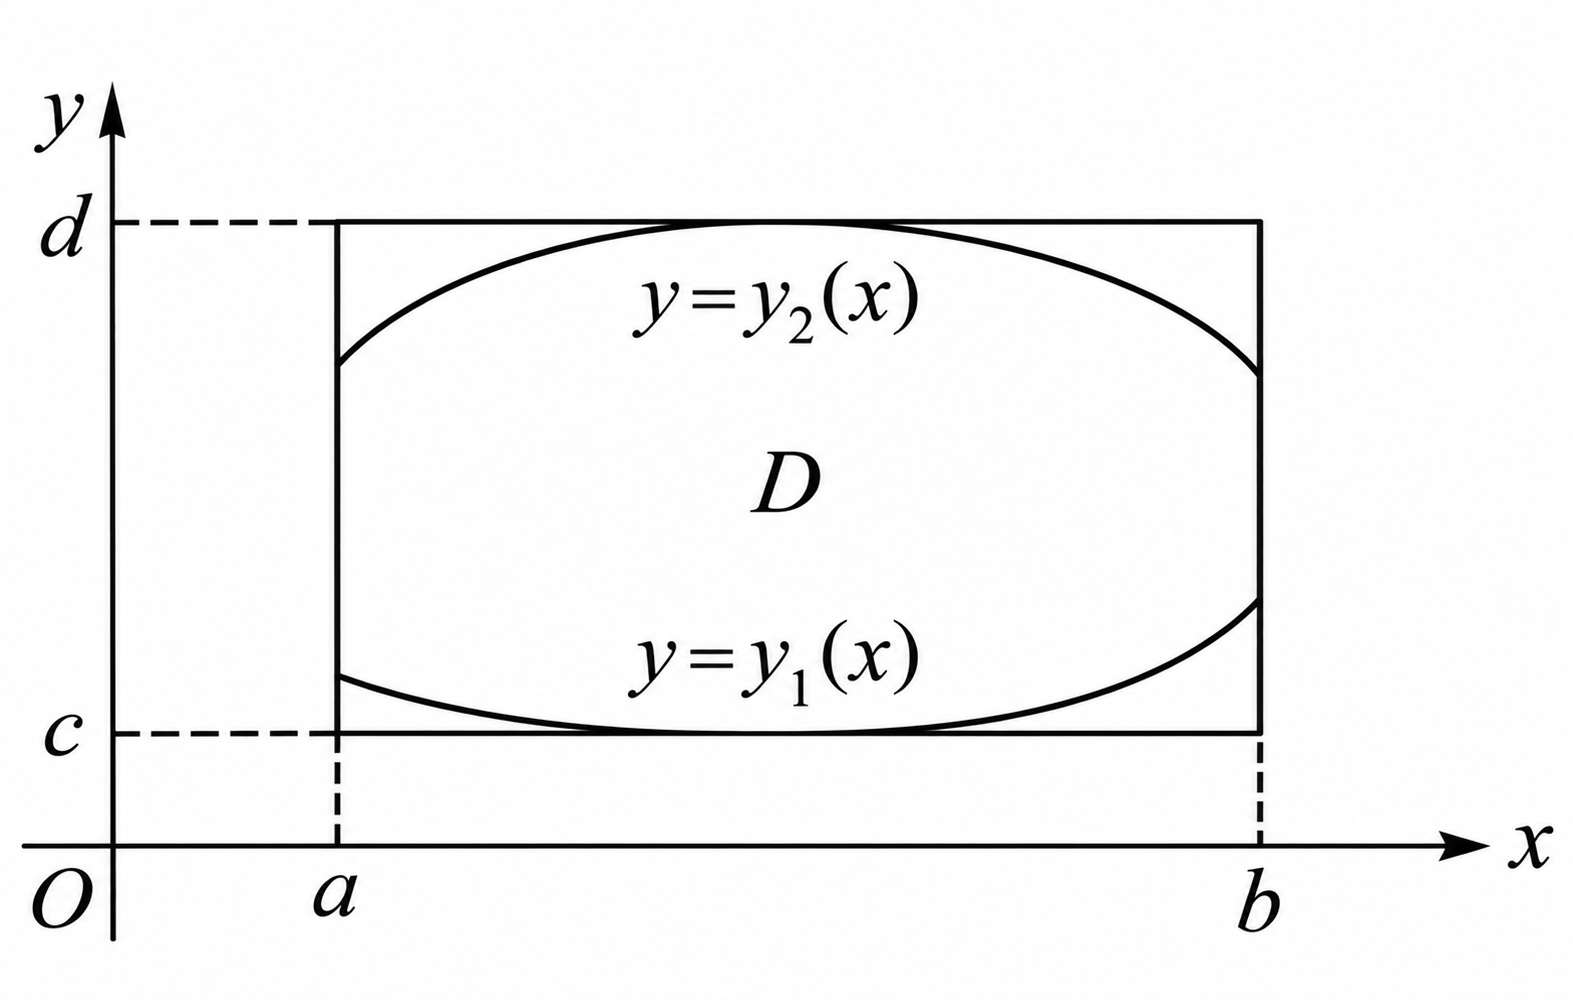
\includegraphics[width=0.5\textwidth]{figure/P2/section2_general_region_hd.png}
\end{center}

令
\[
\widetilde f(x,y)=
\begin{cases}
f(x,y),&(x,y)\in D,\\
0,&(x,y)\in\widetilde D\setminus D.
\end{cases}
\]
$\widetilde f$ 在 $\widetilde D$ 上可积，因为它只可能在零面积边界
$\partial D$ 处不连续。
注意到 $\widetilde f$ 在 $D$ 外为零，对固定的 $x$，
\[
\begin{aligned}
\int_c^d\widetilde f(x,y)\,\dd y
&=\int_c^{y_1(x)}\widetilde f(x,y)\,\dd y
+\int_{y_1(x)}^{y_2(x)}\widetilde f(x,y)\,\dd y
+\int_{y_2(x)}^d\widetilde f(x,y)\,\dd y\\
&=\int_{y_1(x)}^{y_2(x)}f(x,y)\,\dd y.
\end{aligned}
\]
由于 $f$ 在 $D$ 上连续，上式对每个 $x\in[a,b]$ 都有定义。
因此
\[
\begin{aligned}
\iint_D f(x,y)\,\dd x\,\dd y
&=\iint_{\widetilde D}\widetilde f(x,y)\,\dd x\,\dd y\\
&=\int_a^b\dd x\int_c^d\widetilde f(x,y)\,\dd y\\
&=\int_a^b\dd x\int_{y_1(x)}^{y_2(x)}f(x,y)\,\dd y.
\end{aligned}
\]

类似地，若 $f$ 在
\[
D=\{(x,y):x_1(y)\le x\le x_2(y),\ c\le y\le d\}
\]
上连续，且 $x_1,x_2$ 在 $[c,d]$ 上连续，则
\[
\iint_D f(x,y)\,\dd x\,\dd y
=\int_c^d\dd y\int_{x_1(y)}^{x_2(y)}f(x,y)\,\dd x.
\]
\subsubsection*{三重积分}
若积分区域为长方体
\[
D=[a,b]\times[c,d]\times[e,f],
\]
则可以按照前面的累次积分公式计算三重积分。

对于一般区域 $\Omega$，一种方法是投影法，
另一种方法是截面法。

\textbf{投影法：}在三维情形，若 $f(x,y,z)$ 在
\[
\Omega=\{(x,y,z):
z_1(x,y)\le z\le z_2(x,y),\
y_1(x)\le y\le y_2(x),\
a\le x\le b\}
\]
上连续，且 $z_1,z_2,y_1,y_2$ 都连续，则
\[
\begin{aligned}
\iiint_\Omega f(x,y,z)\,\dd x\,\dd y\,\dd z
&=\iint_{\Omega_{xy}}\dd x\,\dd y
\int_{z_1(x,y)}^{z_2(x,y)}f(x,y,z)\,\dd z\\
&=\int_a^b\dd x\int_{y_1(x)}^{y_2(x)}\dd y
\int_{z_1(x,y)}^{z_2(x,y)}f(x,y,z)\,\dd z,
\end{aligned}
\]
其中
\[
\Omega_{xy}=\{(x,y):y_1(x)\le y\le y_2(x),\ a\le x\le b\}
\]
为区域 $\Omega$ 在 $xy$ 平面上的投影。

\begin{center}
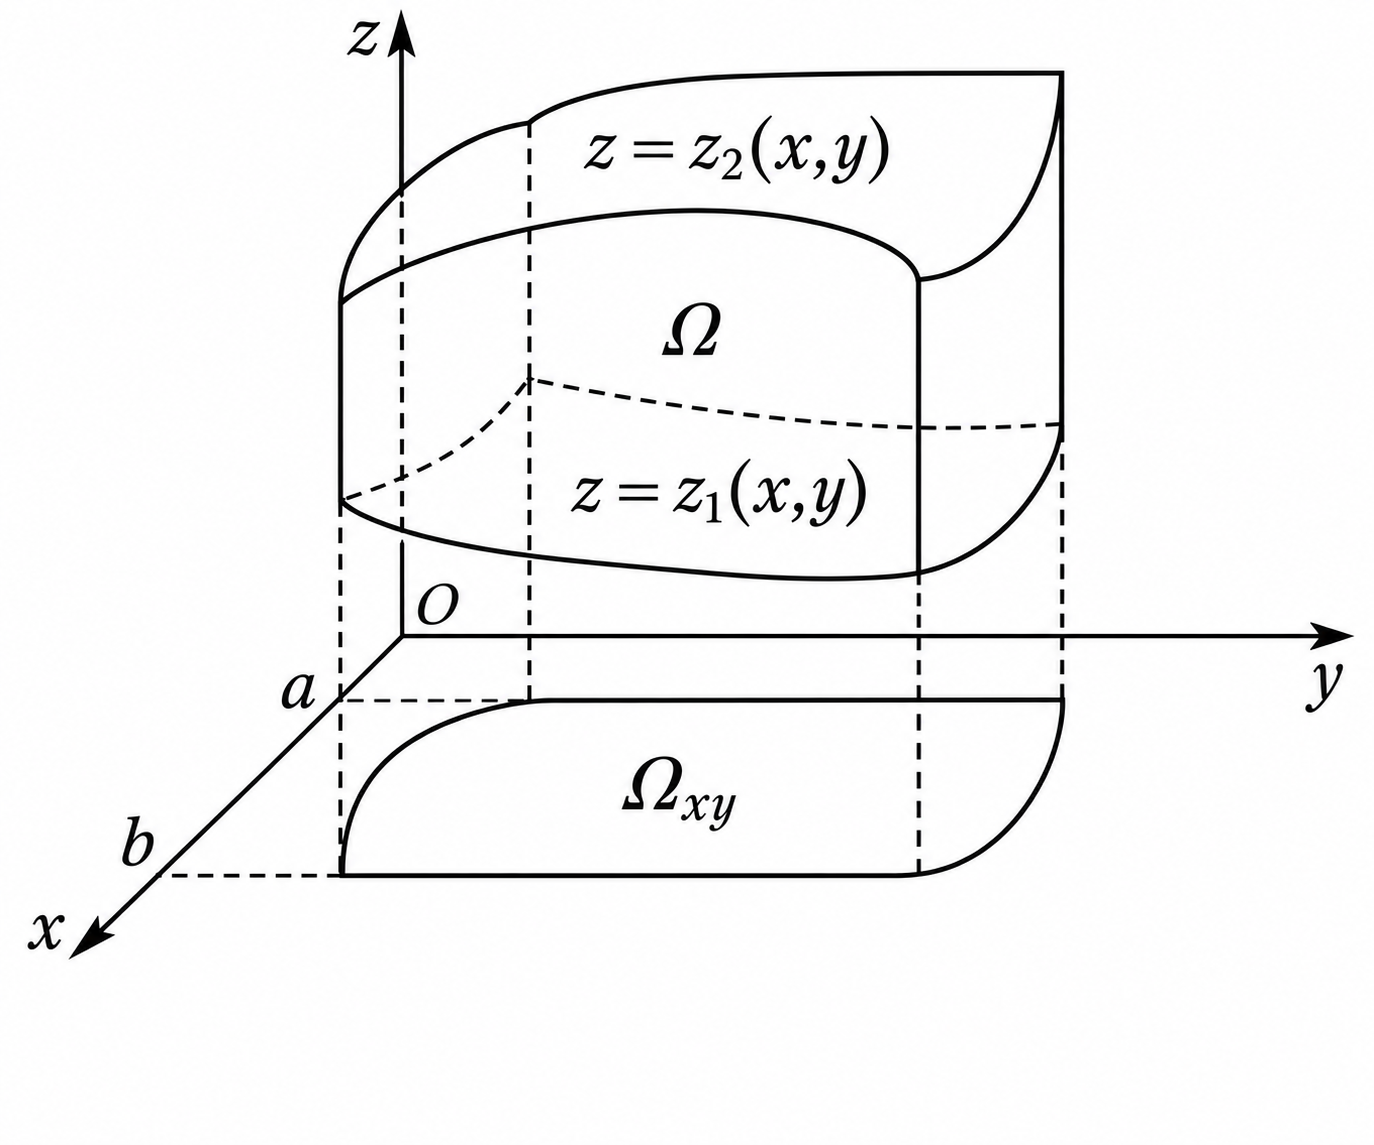
\includegraphics[width=0.5\textwidth]{figure/P2/section2_solid_hd.png}
\end{center}

\textbf{截面法：}设 $\Omega$ 夹在平面 $z=e$ 与 $z=f$ 之间，其中 $e\le f$。
固定 $z$，用平面 $z=\text{常数}$ 截取 $\Omega$，
并将所得截面投影到 $xy$ 平面，记投影区域为 $\Omega'_z$。
在相应积分存在的条件下，有
\[
\iiint_\Omega f(x,y,z)\,\dd x\,\dd y\,\dd z
=\int_e^f\dd z\iint_{\Omega'_z}f(x,y,z)\,\dd x\,\dd y.
\]
这里内层积分中的 $z$ 是固定的参数。

\begin{center}
% 截面法示意：固定 z，再把截面投影到 xy 平面。
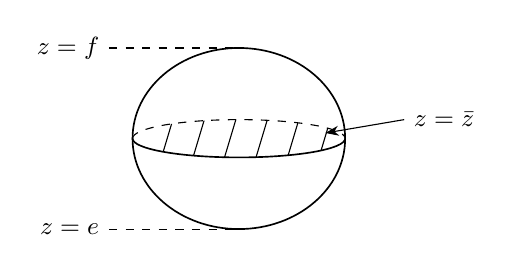
\begin{tikzpicture}[>=Stealth,font=\small]
  \draw[line width=.6pt] (0,0) ellipse[x radius=1.35,y radius=1.15];
  \draw[dashed] (-1.35,0) arc[start angle=180,end angle=0,x radius=1.35,y radius=.24];
  \draw[line width=.6pt] (-1.35,0) arc[start angle=180,end angle=360,x radius=1.35,y radius=.24];
  \begin{scope}
    \clip (0,0) ellipse[x radius=1.35,y radius=.24];
    \foreach \s in {-1,-.6,-.2,.2,.6,1}
      \draw[thin] (\s,-.3) -- ({\s+.18},.3);
  \end{scope}
  \draw[dashed] (-1.65,1.15) -- (0,1.15);
  \draw[dashed] (-1.65,-1.15) -- (0,-1.15);
  \node[left] at (-1.65,1.15) {$z=f$};
  \node[left] at (-1.65,-1.15) {$z=e$};
  \draw[->] (2.1,.24) -- (1.1,.07);
  \node[right] at (2.1,.24) {$z=\bar z$};
\end{tikzpicture}

\end{center}

\begin{example}[非均匀金属块的质量]
一非均匀金属块在空间中的表示是由双曲抛物面 $z=xy$、
平面 $x+y=1$ 和 $z=0$ 所围成的区域 $\Omega$，
其密度函数为 $\rho(x,y,z)=xy$，求它的质量。
\end{example}
\begin{solution}
由图，$\Omega$ 可表示为
\[
\Omega=\{(x,y,z):0\le z\le xy,\ 0\le y\le1-x,\ 0\le x\le1\}.
\]

\begin{center}
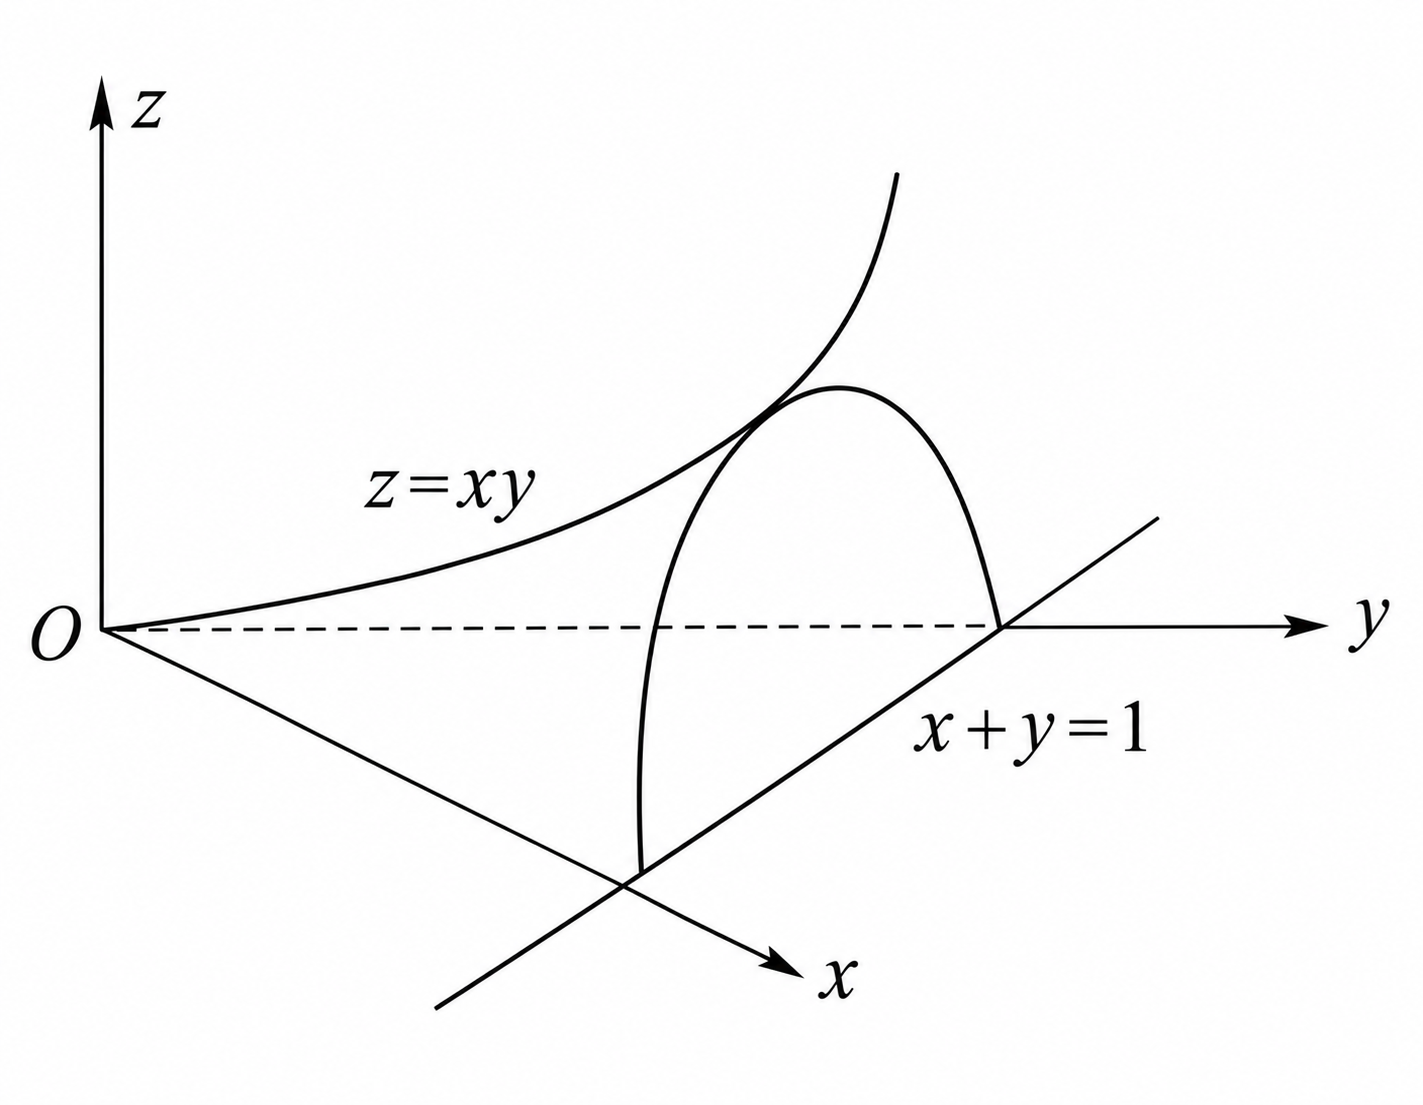
\includegraphics[width=0.45\textwidth]{figure/P2/sec2_metal_source_hd.png}
\end{center}

因此金属块的质量为
\[
\begin{aligned}
M
&=\iiint_\Omega\rho(x,y,z)\,\dd x\,\dd y\,\dd z=\int_0^1\dd x\int_0^{1-x}\dd y\int_0^{xy}xy\,\dd z=\int_0^1\dd x\int_0^{1-x}x^2y^2\,\dd y\\
&=\frac13\int_0^1x^2(1-x)^3\,\dd x=\frac13\left(\frac13-\frac34+\frac35-\frac16\right)=\frac1{180}.
\end{aligned}
\]
\end{solution}

\begin{example}[用截面法计算圆锥上的积分]
计算
\[
I=\iiint_\Omega z^2\,\dd x\,\dd y\,\dd z,
\]
其中 $\Omega$ 是由锥面
\[
z^2=\frac{h^2}{R^2}(x^2+y^2)
\]
与平面 $z=h$ 所围成的闭区域，$R>0$、$h>0$。
\end{example}
\begin{solution}
这里的 $\Omega$ 可表示为
\[
\Omega=\left\{(x,y,z):
0\le z\le h,\quad
\frac{h^2}{R^2}(x^2+y^2)\le z^2\right\}.
\]

\begin{center}
% 圆锥 z^2=(h^2/R^2)(x^2+y^2) 的上半部。
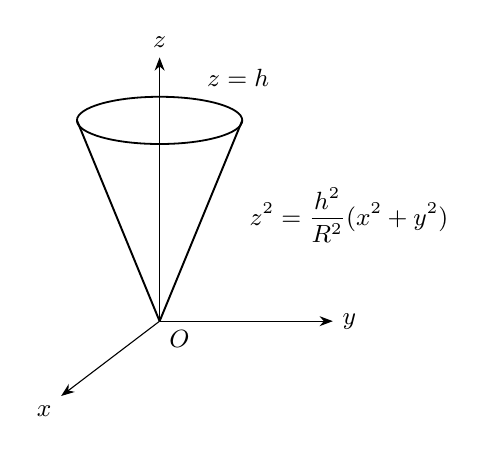
\begin{tikzpicture}[>=Stealth,font=\small,line join=round]
  \draw[->] (0,0) -- (2.2,0) node[right] {$y$};
  \draw[->] (0,0) -- (-1.25,-.95) node[below left] {$x$};
  \draw[->] (0,0) -- (0,3.35) node[above] {$z$};
  \draw[line width=.7pt] (0,0) -- (-1.05,2.55);
  \draw[line width=.7pt] (0,0) -- (1.05,2.55);
  \draw[line width=.65pt] (0,2.55) ellipse[x radius=1.05,y radius=.3];
  \node[below right] at (0,0) {$O$};
  \node[above right] at (.48,2.85) {$z=h$};
  \node[right,align=left] at (1.02,1.35)
    {$\displaystyle z^2=\frac{h^2}{R^2}(x^2+y^2)$};
\end{tikzpicture}

\end{center}

固定 $z\in[0,h]$。
用过点 $(0,0,z)$ 且平行于 $xy$ 平面的平面截取 $\Omega$，
所得截面在 $xy$ 平面上的投影为圆盘
\[
\Omega'_z
=\left\{(x,y):x^2+y^2\le\frac{R^2}{h^2}z^2\right\}.
\]
其半径为 $Rz/h$，所以
\[
\iint_{\Omega'_z}\dd x\,\dd y
=\pi\frac{R^2}{h^2}z^2.
\]

由截面法，
\[
\begin{aligned}
I
&=\int_0^h\dd z\iint_{\Omega'_z}z^2\,\dd x\,\dd y\\
&=\int_0^h z^2
\left(\iint_{\Omega'_z}\dd x\,\dd y\right)\dd z\\
&=\frac{\pi R^2}{h^2}\int_0^h z^4\,\dd z\\
&=\frac{\pi R^2h^3}{5}.
\end{aligned}
\]
\end{solution}

%
% 第3节：重积分的变量代换
% !TEX root = ../../../main.tex
% 所属：第二部分：多变量分析学 / 第3章：重积分
% 节：3.3 重积分的变量代换
% 正文按原文件顺序保存；由 ../chapter3.tex 调用。
\section{重积分的变量代换}
\subsection*{二重积分的变量代换}

\begin{definition}
	设 $U\subset\R^2$ 为开集，考虑映射
\[
T:U\longrightarrow V=T(U),\qquad
(u,v)\longmapsto\bigl(x(u,v),y(u,v)\bigr).
\]
要求 $T$ 为一一映射，并满足：
\begin{enumerate}
\item $x(u,v)$、$y(u,v)$ 在 $U$ 上连续可导；
\item Jacobian 行列式
\[
\frac{\partial(x,y)}{\partial(u,v)}
=\begin{vmatrix}
\dfrac{\partial x}{\partial u}&\dfrac{\partial x}{\partial v}\\[5pt]
\dfrac{\partial y}{\partial u}&\dfrac{\partial y}{\partial v}
\end{vmatrix}
\ne0.
\]
\end{enumerate}
这样的 $T$ 是 $U$ 到 $V$ 的一个微分同胚，称$T$为平面上的一个坐标变换。
\end{definition}

在 $U$ 中取直线 $u=u_0$，它在 $xy$ 平面中对应一条曲线
\[
x=x(u_0,v),\qquad y=y(u_0,v),
\]
称为 $v$-曲线。
同样，直线 $v=v_0$ 对应曲线
\[
x=x(u,v_0),\qquad y=y(u,v_0),
\]
称为 $u$-曲线。

由于 $T$ 为一一映射，$V$ 中的每一点既可唯一地用 $(x,y)$ 表示，
也可唯一地用 $(u,v)$ 表示。
称这些 $u$-曲线和 $v$-曲线构成曲线坐标网，
称 $(u,v)$ 为该点的曲线坐标。

\begin{center}
% 直线坐标网与曲线坐标网；固定 u 得到 v-曲线，固定 v 得到 u-曲线。
\begin{tikzpicture}[>=Stealth,font=\small]
  \begin{scope}
    \draw[->] (0,0) -- (3.15,0) node[right] {$u$};
    \draw[->] (0,0) -- (0,2.8) node[above] {$v$};
    \node[below left] at (0,0) {$O$};
    \foreach \u in {.85,1.45} \draw[gray] (\u,.25) -- (\u,2.4);
    \foreach \v in {.8,1.4} \draw[gray] (.3,\v) -- (2.65,\v);
    \node[above] at (.85,2.4) {$u=u_0$};
    \node[right] at (2.65,.8) {$v=v_0$};
  \end{scope}
  \draw[->] (3.55,1.45) -- (4.35,1.45) node[midway,above] {$T$};
  \begin{scope}[xshift=5cm]
    \draw[->] (0,0) -- (3.35,0) node[right] {$x$};
    \draw[->] (0,0) -- (0,2.8) node[above] {$y$};
    \node[below left] at (0,0) {$O$};
    \foreach \u in {.6,1.25,1.9}{
      \draw[domain=.3:2.15,samples=35,variable=\v]
        plot ({\u+.16*\v*\v},{\v+.08*\u*\u});
    }
    \foreach \v in {.65,1.25,1.85}{
      \draw[domain=.35:2.6,samples=35,variable=\u]
        plot ({\u+.16*\v*\v},{\v+.08*\u*\u});
    }
    \node[right] at (2.7,1.35) {$u$-曲线};
    \node[above] at (2.65,2.5) {$v$-曲线};
  \end{scope}
\end{tikzpicture}

\end{center}

\begin{theorem}[二重积分的变量代换]\label{p2-double-change-of-variables}
设 $U$ 是 $uv$ 平面上的开集，
\[
T:U\longrightarrow T(U),\qquad
(u,v)\longmapsto\bigl(x(u,v),y(u,v)\bigr)
\]
为一一映射。
设 $x(u,v)$、$y(u,v)$ 在 $U$ 上连续可导，且
$\partial(x,y)/\partial(u,v)\ne0$。
若 $D\subset U$ 为有界零边界闭区域，$f$ 在 $T(D)$ 上连续，则
\[
\iint_{T(D)}f(x,y)\,\dd x\,\dd y
=\iint_D f\bigl(x(u,v),y(u,v)\bigr)
\left|\frac{\partial(x,y)}{\partial(u,v)}\right|
\,\dd u\,\dd v.
\]
\end{theorem}
% 变量代换定理的补充证明见本节末。

\subsection*{变量代换的例子}

在下面的例子中，原来的 $xy$ 平面区域记为 $D$，
对应的参数平面区域记为 $D'$，即 $T(D')=D$。

\begin{example}[线性代换计算面积]
设 $a>0$，求曲线 $(x-y)^2+x^2=a^2$ 所围区域的面积。
\end{example}
\begin{solution}
原区域为
\[
D=\{(x,y):(x-y)^2+x^2\le a^2\},
\qquad
S_D=\iint_D\dd x\,\dd y.
\]
令
\[
u=x,\qquad v=x-y.
\]
则逆变换为
\[
x=u,\qquad y=u-v,
\]
并且
\[
\frac{\partial(x,y)}{\partial(u,v)}
=\begin{vmatrix}1&0\\1&-1\end{vmatrix}=-1.
\]
由于
\[
(x-y)^2+x^2=u^2+v^2,
\]
原区域对应圆盘
\[
D'=\{(u,v):u^2+v^2\le a^2\}.
\]
因此
\[
S_D=\iint_{D'}1\,\dd u\,\dd v=\pi a^2.
\]
\end{solution}

\begin{example}[双曲线与射线围成区域的面积]
设 $0<a<b$、$0<p<q$，求第一象限内由
\[
xy=p,\qquad xy=q,\qquad y=ax,\qquad y=bx
\]
围成的区域 $D$ 的面积。
\end{example}
\begin{solution}

\begin{center}
% xy=p、xy=q、y=ax、y=bx 围成的第一象限区域。
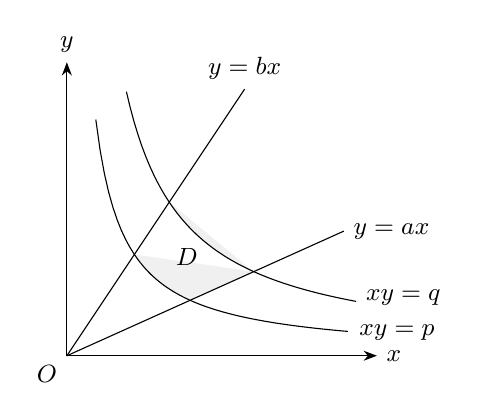
\begin{tikzpicture}[>=Stealth,font=\small,scale=1.05]
  \draw[->] (0,0) -- (3.75,0) node[right] {$x$};
  \draw[->] (0,0) -- (0,3.55) node[above] {$y$};
  \node[below left] at (0,0) {$O$};
  \fill[gray!12]
    (.816497,1.224745)
    plot[domain=.816497:1.490712,samples=35] (\x,{1/\x})
    -- (2.260777,1.017350)
    plot[domain=2.260777:1.238278,samples=35] (\x,{2.3/\x})
    -- cycle;
  \draw[domain=.35:3.4,samples=60] plot (\x,{1/\x});
  \draw[domain=.72:3.5,samples=60] plot (\x,{2.3/\x});
  \draw (0,0) -- (3.35,1.5075) node[right] {$y=ax$};
  \draw (0,0) -- (2.15,3.225) node[above] {$y=bx$};
  \node[right] at (3.42,.28) {$xy=p$};
  \node[right] at (3.5,.7) {$xy=q$};
  \node at (1.45,1.2) {$D$};
\end{tikzpicture}

\end{center}

令
\[
u=xy,\qquad v=\frac yx.
\]
由于 $x,y>0$，可解得
\[
x=\sqrt{\frac uv},\qquad y=\sqrt{uv}.
\]
原区域变为矩形
\[
D'=\{(u,v):p\le u\le q,\ a\le v\le b\}.
\]
计算 Jacobian 行列式：
\[
\begin{aligned}
\frac{\partial(x,y)}{\partial(u,v)}
&=\begin{vmatrix}
\dfrac1{2\sqrt{uv}}&-\dfrac12\sqrt{\dfrac u{v^3}}\\[7pt]
\dfrac12\sqrt{\dfrac vu}&\dfrac12\sqrt{\dfrac uv}
\end{vmatrix}\\
&=\frac1{4v}+\frac1{4v}
=\frac1{2v}.
\end{aligned}
\]
因此
\[
\begin{aligned}
S_D
&=\iint_D\dd x\,\dd y\\
&=\iint_{D'}\frac1{2v}\,\dd u\,\dd v\\
&=\frac12\int_p^q\dd u\int_a^b\frac1v\,\dd v\\
&=\frac12\int_p^q\ln\frac ba\,\dd u\\
&=\frac{q-p}{2}\ln\frac ba.
\end{aligned}
\]

\end{solution}

\subsection*{极坐标变换}

对于含有 $x^2+y^2$ 的表达式，可以考虑极坐标变换
\[
x=r\cos\theta,\qquad y=r\sin\theta.
\]
其 Jacobian 行列式为
\[
\frac{\partial(x,y)}{\partial(r,\theta)}
=\begin{vmatrix}
\cos\theta&-r\sin\theta\\
\sin\theta&r\cos\theta
\end{vmatrix}
=r.
\]
例如，圆域 $x^2+y^2<a^2$ 在参数平面中对应
$0<r<a$、$0<\theta<2\pi$，另需处理原点和角度接缝。
\textbf{半径约定：}本段用 $a$ 表示圆域半径，
所以写成 $x^2+y^2<a^2$，与径向上限 $r<a$ 相对应。

注意，当 $r=0$ 时，极坐标变换不是一一对应的。
在应用变量代换公式时，还需避开角度接缝，即在 $xy$ 平面中去掉非负实轴。
可以先在避开这些点的区域上应用公式，再取极限。

\begin{example}[圆域上的极坐标积分]
计算
\[
I=\iint_D\sin\!\left(\pi\sqrt{x^2+y^2}\right)\,\dd x\,\dd y,
\qquad
D=\{(x,y):x^2+y^2\le1\}.
\]
\end{example}
\begin{solution}
引入极坐标 $x=r\cos\theta$、$y=r\sin\theta$。
形式上，$D$ 对应参数区域
\[
D_1=\{(r,\theta):0\le r\le1,\ 0\le\theta\le2\pi\}.
\]
于是
\[
\begin{aligned}
&=\iint_{D_1}(\sin\pi r)\,r\,\dd r\,\dd\theta\\
&=\int_0^{2\pi}\dd\theta\int_0^1r\sin\pi r\,\dd r\\
&=2\pi\left[-\frac r\pi\cos\pi r
+\frac{\sin\pi r}{\pi^2}\right]_0^1\\
&=2.
\end{aligned}
\]

严格地说，需先避开原点和非负实轴。
对充分小的 $\varepsilon>0$，取参数矩形
\[
D_{1,\varepsilon}
=\{(r,\theta):\varepsilon\le r\le1,\
\varepsilon\le\theta\le2\pi-\varepsilon\},
\]
并记其在 $xy$ 平面中的像为 $D_\varepsilon$。
在这个参数矩形上，极坐标变换是一一的，且 Jacobian 行列式不为零。

\begin{center}
% 极坐标下避开原点与角度接缝：参数矩形对应去心扇环。
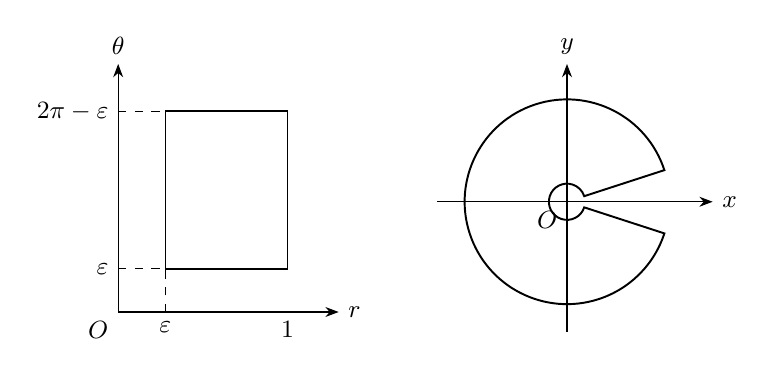
\begin{tikzpicture}[>=Stealth,font=\small]
  \begin{scope}
    \draw[->] (0,0) -- (2.8,0) node[right] {$r$};
    \draw[->] (0,0) -- (0,3.15) node[above] {$\theta$};
    \node[below left] at (0,0) {$O$};
    \draw[line width=.65pt] (.6,.55) rectangle (2.15,2.55);
    \draw[dashed] (0,.55) -- (.6,.55);
    \draw[dashed] (0,2.55) -- (.6,2.55);
    \draw[dashed] (.6,0) -- (.6,.55);
    \node[left] at (0,.55) {$\varepsilon$};
    \node[left] at (0,2.55) {$2\pi-\varepsilon$};
    \node[below] at (.6,0) {$\varepsilon$};
    \node[below] at (2.15,0) {$1$};
  \end{scope}
  \begin{scope}[xshift=5.7cm,yshift=1.4cm]
    \draw[->] (-1.65,0) -- (1.85,0) node[right] {$x$};
    \draw[->] (0,-1.65) -- (0,1.75) node[above] {$y$};
    \node[below left] at (0,0) {$O$};
    \draw[line width=.7pt]
      (18:1.3) arc[start angle=18,end angle=342,radius=1.3]
      -- (342:.23) arc[start angle=342,end angle=18,radius=.23]
      -- cycle;
  \end{scope}
\end{tikzpicture}

\end{center}

因此，按原图避开接缝后取极限的步骤，
\[
\begin{aligned}
I
&=\lim_{\varepsilon\to0^+}
\iint_{D_\varepsilon}
\sin\!\left(\pi\sqrt{x^2+y^2}\right)\,\dd x\,\dd y\\
&=\lim_{\varepsilon\to0^+}
\int_\varepsilon^{2\pi-\varepsilon}\dd\theta
\int_\varepsilon^1r\sin\pi r\,\dd r\\
&=\lim_{\varepsilon\to0^+}
(2\pi-2\varepsilon)
\left[-\frac r\pi\cos\pi r
+\frac{\sin\pi r}{\pi^2}\right]_\varepsilon^1\\
&=2.
\end{aligned}
\]

\textbf{补充说明：}记本例的被积函数为
$f(x,y)=\sin(\pi\sqrt{x^2+y^2})$。
上面取极限的依据是，$|f(x,y)|\le1$，
而删去的部分包含于半径为 $\varepsilon$ 的圆盘
以及总角度为 $2\varepsilon$ 的单位圆扇形之并。
所以
\[
\left|\iint_D f\,\dd x\,\dd y
-\iint_{D_\varepsilon}f\,\dd x\,\dd y\right|
\le m(D\setminus D_\varepsilon)
\le\pi\varepsilon^2+\varepsilon\longrightarrow0.
\]
\end{solution}

\subsubsection*{广义极坐标变换}

对于椭圆
\[
\frac{x^2}{a^2}+\frac{y^2}{b^2}\le1,
\qquad a>0,\ b>0,
\]
可取
\[
x=ar\cos\theta,\qquad y=br\sin\theta.
\]
相应的参数范围为 $0\le r\le1$、$0\le\theta\le2\pi$，
且
\[
\frac{\partial(x,y)}{\partial(r,\theta)}
=\begin{vmatrix}
a\cos\theta&-ar\sin\theta\\
b\sin\theta&br\cos\theta
\end{vmatrix}
=abr.
\]

\subsubsection*{平移后的极坐标变换}

例如，对于圆域
\[
(x-x_0)^2+(y-y_0)^2\le a^2,
\]
可先平移坐标，再作极坐标变换：
\[
x=x_0+r\cos\theta,\qquad
y=y_0+r\sin\theta.
\]
参数区域为 $0\le r\le a$、$0\le\theta\le2\pi$，
原点和角度接缝按前述方法处理。

\begin{center}
% 平移后的圆域与极坐标参数矩形。
\begin{tikzpicture}[>=Stealth,font=\small]
  \begin{scope}
    \draw[->] (0,0) -- (3.1,0) node[right] {$x$};
    \draw[->] (0,0) -- (0,2.8) node[above] {$y$};
    \node[below left] at (0,0) {$O$};
    \draw[line width=.65pt] (1.55,1.6) circle[radius=.7];
    \fill (1.55,1.6) circle[radius=.025];
    \node[below,font=\scriptsize] at (1.55,1.45) {$(x_0,y_0)$};
  \end{scope}
  \draw[->] (3.5,1.3) -- (4.3,1.3);
  \begin{scope}[xshift=5cm]
    \draw[->] (0,0) -- (2.9,0) node[right] {$r$};
    \draw[->] (0,0) -- (0,2.8) node[above] {$\theta$};
    \node[below left] at (0,0) {$O$};
    \draw[line width=.65pt] (0,0) rectangle (1.85,2.15);
    \node[left] at (0,2.15) {$2\pi$};
    \node[below] at (1.85,0) {$a$};
  \end{scope}
\end{tikzpicture}

\end{center}

\subsection*{变量代换定理的证明}



\subsubsection*{内外矩形逼近与零面积集的像}

取一个包含 $D$ 的闭矩形 $S$。
把它的两边不断二等分，得到一列逐次加细的矩形网格，网格的模长趋于零。
记完全包含于 $D$ 的小矩形之并为 $A_n$，
与 $D$ 相交的小矩形之并为 $B_n$，则
\[
A_n\subset A_{n+1}\subset D\subset B_{n+1}\subset B_n.
\]
由 $D$ 可求面积，
\[
mA_n\longrightarrow mD,\qquad mB_n\longrightarrow mD,
\qquad mB_n-mA_n\longrightarrow0.
\]
特别地，把与 $D$ 相交但不完全包含于 $D$ 的网格小矩形记为 $R_j$，则
\[
\sum_jmR_j=mB_n-mA_n\longrightarrow0.
\]
这些闭矩形只在零面积的边界上重叠，因此这里的面积相加不会重复计算正面积部分。
虽然 $S$ 不一定包含于 $U$，但 $D$ 是 $U$ 中的紧集，
所以充分细的网格中所有与 $D$ 相交的小矩形都包含于 $U$。

\subsubsection*{特殊变换下小矩形的面积}

\begin{lemma}[保留一个坐标的变换]\label{p2-triangular-area}
设 $T$ 是前述坐标变换，并且具有下列形式之一：
\[
T(u,v)=(u,y(u,v)),\qquad T(u,v)=(x(u,v),v).
\]
我们称这样的映射为\textbf{本原映射}.

若闭矩形 $R=[e,f]\times[h,j]$ 包含于 $U$，其中 $e<f$、$h<j$，
则存在 $(\widetilde u,\widetilde v)\in R$，使
\[
mT(R)=|J_T(\widetilde u,\widetilde v)|\,mR.
\]
\end{lemma}
\begin{proof}
先设 $T(u,v)=(u,y(u,v))$。此时 $J_T=y_v\ne0$。
由于 $R$ 连通，$y_v$ 在 $R$ 上符号不变。
先讨论 $y_v>0$ 的情形。

固定 $u$，函数 $v\mapsto y(u,v)$ 严格递增，故
\[
T(R)=\{(x,y):e\le x\le f,\ y(x,h)\le y\le y(x,j)\}.
\]

\[
mT(R)=\int_e^f\bigl(y(x,j)-y(x,h)\bigr)\,\dd x.
\]

\begin{center}
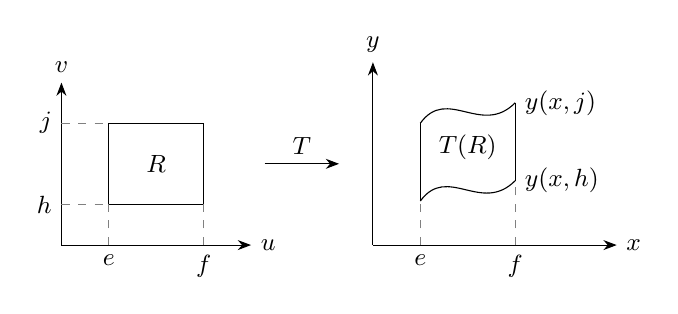
\begin{tikzpicture}[>=Stealth,font=\small,scale=.86]
  \draw[->] (0,0)--(2.8,0) node[right] {$u$};
  \draw[->] (0,0)--(0,2.4) node[above] {$v$};
  \draw (.7,.6) rectangle (2.1,1.8);
  \node[below] at (.7,0) {$e$};
  \node[below] at (2.1,0) {$f$};
  \node[left] at (0,.6) {$h$};
  \node[left] at (0,1.8) {$j$};
  \draw[dashed,gray] (.7,0)--(.7,.6) (2.1,0)--(2.1,.6)
    (0,.6)--(.7,.6) (0,1.8)--(.7,1.8);
  \node at (1.4,1.2) {$R$};
  \draw[->] (3,1.2)--(4.1,1.2) node[midway,above] {$T$};
  \begin{scope}[shift={(4.6,0)}]
    \draw[->] (0,0)--(3.6,0) node[right] {$x$};
    \draw[->] (0,0)--(0,2.7) node[above] {$y$};
    \draw (.7,.65) .. controls (1.1,1.2) and (1.6,.45) .. (2.1,.95);
    \draw (.7,1.8) .. controls (1.1,2.35) and (1.6,1.6) .. (2.1,2.1);
    \draw (.7,.65)--(.7,1.8) (2.1,.95)--(2.1,2.1);
    \draw[dashed,gray] (.7,0)--(.7,.65) (2.1,0)--(2.1,.95);
    \node[below] at (.7,0) {$e$};
    \node[below] at (2.1,0) {$f$};
    \node[right] at (2.1,.95) {$y(x,h)$};
    \node[right] at (2.1,2.1) {$y(x,j)$};
    \node at (1.4,1.45) {$T(R)$};
  \end{scope}
\end{tikzpicture}

\end{center}

先对上面的一元积分应用积分中值定理，再对 $v\mapsto y(\widetilde u,v)$
应用微分中值定理，得到 $\widetilde u\in[e,f]$、$\widetilde v\in(h,j)$，使
\begin{align*}
mT(R)
&=(f-e)\bigl(y(\widetilde u,j)-y(\widetilde u,h)\bigr)\\
&=(f-e)(j-h)y_v(\widetilde u,\widetilde v)\\
&=mR\,|J_T(\widetilde u,\widetilde v)|.
\end{align*}
若 $y_v<0$，交换上下两条边界曲线，便得到相同的绝对值公式。
对于 $T(u,v)=(x(u,v),v)$，交换两个坐标的作用，按同样的步骤证明即可。
\end{proof}

\subsubsection*{由小矩形的面积公式推出积分公式}

\begin{lemma}
	变量代换公式对本原映射成立.
\end{lemma}
\begin{proof}
	仍用第一步中的网格。记完全包含于 $D$ 的小矩形为
$D_1,\ldots,D_{N_n}$，其余与 $D$ 相交的小矩形为 $R_1,\ldots,R_{M_n}$。
令
\[
E_j=D\cap R_j.
\]
这些集合都是零边界紧集；它们及其像都可求面积。
因为 $T$ 是一一映射，它们的像也只在零面积边界上重叠。

对每个 $D_i$，按假设取 $(\widetilde u_i,\widetilde v_i)\in D_i$，使
\[
mT(D_i)=|J_T(\widetilde u_i,\widetilde v_i)|\,mD_i.
\]
再任取 $(a_j,b_j)\in E_j$。由 $T$ 在 $D$ 上一致连续，
当网格的模长趋于零时，上述各像集的直径也一致趋于零。
因此下面两个式子分别是 $f$ 在 $T(D)$ 上以及
$f(x(u,v),y(u,v))|J_T(u,v)|$ 在 $D$ 上的 Riemann 和：
\begin{align*}
S_n
&=\sum_{i=1}^{N_n}
 f\bigl(T(\widetilde u_i,\widetilde v_i)\bigr)mT(D_i)
 +\sum_{j=1}^{M_n}f\bigl(T(a_j,b_j)\bigr)mT(E_j),\\
S'_n
&=\sum_{i=1}^{N_n}
 f\bigl(T(\widetilde u_i,\widetilde v_i)\bigr)
 |J_T(\widetilde u_i,\widetilde v_i)|\,mD_i\\
&\quad+\sum_{j=1}^{M_n}
 f\bigl(T(a_j,b_j)\bigr)|J_T(a_j,b_j)|\,mE_j.
\end{align*}
这里 $T(u,v)$ 写在 $f$ 的自变量位置时，表示有序对
$\bigl(x(u,v),y(u,v)\bigr)$。

记这两个和式的第二部分分别为 $B_n$、$B'_n$。
由小矩形的面积公式，它们的第一部分完全相同，因而
\[
S_n-S'_n=B_n-B'_n.
\]
取常数 $H,K>0$，使 $|f|\le H$、$|J_T|\le K$。
有
\begin{align*}
|B_n|
&\le H\sum_jmT(E_j)
 \le HK\sum_jmR_j\longrightarrow0,\\
|B'_n|
&\le HK\sum_jmE_j
 \le HK\sum_jmR_j\longrightarrow0.
\end{align*}
两个被积函数都连续，而相应积分区域均为零边界紧集，所以它们都可积。
令网格模长趋于零，就得到
\begin{equation}\label{p2-triangular-substitution}
\iint_{T(D)}f(x,y)\,\dd x\,\dd y
=\iint_D f\bigl(x(u,v),y(u,v)\bigr)|J_T(u,v)|\,\dd u\,\dd v.
\end{equation}
\end{proof}



\subsubsection*{一般变换的局部分解}

\begin{lemma}[局部分解]\label{p2-local-triangular-factorization}
在定理 \ref{p2-double-change-of-variables} 的条件下，
对每个 $(u_0,v_0)\in U$，适当交换自变量或像坐标的次序后，
可以在 $(u_0,v_0)$ 的一个邻域内将 $T$ 分解为
\[
T=T_2\circ T_1,
\]
其中 $T_1$、$T_2$ 都是本原映射.
\end{lemma}
\begin{proof}
因为 $J_T(u_0,v_0)\ne0$，四个一阶偏导数中至少有一个非零。
适当交换坐标后，可设 $x_u(u_0,v_0)\ne0$。
由连续性，缩小邻域后可使 $x_u$ 在其中处处非零。

令
\[
T_1:\quad \xi=x(u,v),\qquad \eta=v.
\]
其 Jacobian 为 $x_u\ne0$。由反函数定理，进一步缩小邻域后，
$T_1$ 有连续可导的逆映射，可写为
\[
u=g(\xi,\eta),\qquad v=\eta.
\]
再令
\[
T_2:\quad x=\xi,\qquad y=y\bigl(g(\xi,\eta),\eta\bigr).
\]
这就得到 $T_2\circ T_1=T$。

对恒等式 $x(g(\xi,\eta),\eta)=\xi$ 求偏导，得到
\[
g_\xi=\frac1{x_u},\qquad g_\eta=-\frac{x_v}{x_u}.
\]
所以
\begin{align*}
\frac{\partial(x,y)}{\partial(\xi,\eta)}
&=\frac{\partial}{\partial\eta}
 y\bigl(g(\xi,\eta),\eta\bigr)\\
&=y_ug_\eta+y_v
 =\frac{x_uy_v-x_vy_u}{x_u}
 =\frac{J_T}{x_u}\ne0.
\end{align*}
上式右边的偏导数均在 $(u,v)=(g(\xi,\eta),\eta)$ 处取值。
$T_2=T\circ T_1^{-1}$ 也是一一映射，故两个映射都满足所需条件。
坐标交换的 Jacobian 的绝对值为 $1$，不会改变最后公式中的绝对值因子。
\end{proof}

设 $D'$ 是上述分解邻域内的任意零边界紧集。
先对 $T_2$ 使用已经证明的特殊情形，再对 $T_1$ 使用一次，得到
\begin{align*}
\iint_{T(D')}f(x,y)\,\dd x\,\dd y
&=\iint_{T_1(D')}
 f\bigl(T_2(\xi,\eta)\bigr)
 \left|\frac{\partial(x,y)}{\partial(\xi,\eta)}\right|
 \,\dd\xi\,\dd\eta\\
&=\iint_{D'} f\bigl(T(u,v)\bigr)
 \left|\frac{\partial(x,y)}{\partial(\xi,\eta)}
       \frac{\partial(\xi,\eta)}{\partial(u,v)}\right|
 \,\dd u\,\dd v\\
&=\iint_{D'}f\bigl(T(u,v)\bigr)|J_T(u,v)|\,\dd u\,\dd v.
\end{align*}
第二行中的第一个 Jacobian 要在 $(\xi,\eta)=T_1(u,v)$ 处取值；
最后一步使用了复合映射的 Jacobian 乘法公式。
这样就证明了变量代换公式的局部形式。

\subsubsection*{有限覆盖与整体公式}

\begin{proof}[定理 \ref{p2-double-change-of-variables} 的证明]
对每个 $p\in D$，按局部分解引理取开邻域 $U_p\subset U$，
使刚才的局部公式在 $U_p$ 内成立。
再取 $r_p>0$，使开球 $O(p,2r_p)\subset U_p$。
开球族 $\{O(p,r_p):p\in D\}$ 覆盖紧集 $D$。
由 Heine--Borel 定理，可取有限子覆盖
\[
D\subset\bigcup_{k=1}^sO(p_k,r_{p_k}).
\]
令
\[
\delta=\min_{1\le k\le s}r_{p_k}>0.
\]

用直径小于 $\delta$ 的网格小矩形 $Q_j$ 分割 $D$，记 $D_j=D\cap Q_j$，
忽略空集。
任取 $q\in D_j$，存在 $k$ 使 $q\in O(p_k,r_{p_k})$。
对任意 $q'\in D_j$，有
\[
|q'-p_k|\le|q'-q|+|q-p_k|<\delta+r_{p_k}\le2r_{p_k}.
\]
因此 $D_j\subset O(p_k,2r_{p_k})\subset U_{p_k}$，
可以在每个 $D_j$ 上使用局部公式。

各 $D_j$ 的公共部分都在网格分割线上，面积为零，
其像的面积也为零。
对有限个小块的局部公式求和，并利用积分的区域可加性，得到
\begin{align*}
\iint_{T(D)}f(x,y)\,\dd x\,\dd y
&=\sum_j\iint_{T(D_j)}f(x,y)\,\dd x\,\dd y\\
&=\sum_j\iint_{D_j}
 f\bigl(x(u,v),y(u,v)\bigr)|J_T(u,v)|\,\dd u\,\dd v\\
&=\iint_D f\bigl(x(u,v),y(u,v)\bigr)
 \left|\frac{\partial(x,y)}{\partial(u,v)}\right|\,\dd u\,\dd v.
\end{align*}
这就完成了定理的证明。
\end{proof}

\subsection*{高维情形与柱面、球面坐标}

\begin{theorem}[重积分的变量代换]
设 $U\subset\R^n$ 为开集，$T:U\to V=T(U)$ 为一一映射，
\[
T:\quad y_i=y_i(x_1,\ldots,x_n),\qquad i=1,\ldots,n.
\]
设各 $y_i$ 连续可导，且 Jacobian 行列式处处非零。
其逆映射也连续可导，记为
\[
x_i=x_i(y_1,\ldots,y_n),\qquad i=1,\ldots,n.
\]
由逆映射的链式法则，
\[
\frac{\partial(x_1,\ldots,x_n)}{\partial(y_1,\ldots,y_n)}\bigl(T(x)\bigr)
=\left(\frac{\partial(y_1,\ldots,y_n)}{\partial(x_1,\ldots,x_n)}(x)\right)^{-1}
\ne0.
\]
若 $\Omega\subset U$ 为有界零边界闭区域，$F$ 在 $T(\Omega)$ 上连续，则有
\[
\begin{aligned}
&\int\cdots\int_{T(\Omega)}F(y_1,\ldots,y_n)\,\dd y_1\cdots\dd y_n\\
&\quad=\int\cdots\int_\Omega
 F\bigl(y_1(x),\ldots,y_n(x)\bigr)
 \left|\frac{\partial(y_1,\ldots,y_n)}{\partial(x_1,\ldots,x_n)}\right|
 \,\dd x_1\cdots\dd x_n,
\end{aligned}
\]
其中 $x=(x_1,\ldots,x_n)$。
\end{theorem}
\begin{proof}
先考虑只改变一个坐标的变换
\[
H(t_1,\ldots,t_n)
=(t_1,\ldots,t_{k-1},h(t),t_{k+1},\ldots,t_n),
\qquad h_{t_k}\ne0.
\]
对闭长方体 $Q$，固定其余 $n-1$ 个坐标，
像集沿第 $k$ 个坐标的截面是由两个端点值确定的区间。
由累次积分公式，它的体积是这些区间长度在其余坐标上的积分。
先对这个连续的区间长度用积分中值定理，
再对第 $k$ 个坐标用一元微分中值定理，便得到
\[
mH(Q)=|h_{t_k}(\widetilde t)|\,mQ
=|\det DH(\widetilde t)|\,mQ
\]
对某个 $\widetilde t\in Q$ 成立。

将二维证明中的小正方形换成小正方体，
零体积集的像仍为零体积集：若 $H$ 在紧集附近满足 Lipschitz 估计，
边长为 $a$ 的小正方体的像可用体积不超过
$(2\sqrt nL)^na^n$ 的正方体覆盖。
因此原来的边界估计及 Riemann 和证明逐项适用，
从而得到这种单坐标变换的积分公式。

下面说明一般变换可以局部分解成这些变换。
固定一点，由 Jacobian 矩阵可逆，作适当的像坐标置换后，
可以使各阶顺序主子式在该点都非零。
这是带行选主元的消元法的直接结果。
由连续性，缩小邻域后，这些主子式在邻域内都非零。
定义
\[
S_0(x)=x,\qquad
S_k(x)=\bigl(y_1(x),\ldots,y_k(x),x_{k+1},\ldots,x_n\bigr),
\quad 1\le k\le n.
\]
$S_k$ 的 Jacobian 恰为相应的 $k$ 阶顺序主子式。
由反函数定理，可以取同一个充分小的邻域，使所有 $S_k$ 都有连续可导的逆。
令
\[
H_k=S_k\circ S_{k-1}^{-1}.
\]
$H_k$ 只改变第 $k$ 个坐标，而且 Jacobian 非零。
又有
\[
T=H_n\circ\cdots\circ H_1.
\]
依次使用单坐标变换公式，Jacobian 的绝对值因子相乘，
由链式法则正好得到 $|\det DT|$。
这证明了局部公式。

最后用紧集 $\Omega$ 的有限开覆盖，取足够细的正方体网格，
使每个小块都包含于一个分解邻域。
各小块的公共边界及其像均为零体积集，
对各局部公式求和，便得到整体公式。
\end{proof}

\subsubsection*{柱面与球面坐标变换}

在三维空间中，柱面坐标变换为
\[
x=r\cos\theta,\qquad y=r\sin\theta,\qquad z=z,
\]
其中 $0\le r<+\infty$、$0\le\theta\le2\pi$、$-\infty<z<+\infty$。
计算得
\[
\frac{\partial(x,y,z)}{\partial(r,\theta,z)}
=\begin{vmatrix}
\cos\theta&-r\sin\theta&0\\
\sin\theta&r\cos\theta&0\\
0&0&1
\end{vmatrix}=r.
\]
因此相应的体积元素为 $r\,\dd r\,\dd\theta\,\dd z$。

\begin{center}
\begin{tikzpicture}[>=Stealth,font=\small,
  x={(-.8cm,-.55cm)},y={(1cm,0cm)},z={(0cm,1cm)}]
  \draw[->] (0,0,0)--(2.2,0,0) node[below] {$x$};
  \draw[->] (0,0,0)--(0,2.7,0) node[right] {$y$};
  \draw[->] (0,0,0)--(0,0,2.4) node[above] {$z$};
  \node[above left] at (0,0,0) {$O$};
  \draw (0,0,0)--(1.15,1.8,0)--(1.15,1.8,1.7)--cycle;
  \draw[dashed] (1.15,1.8,0)--(1.15,0,0);
  \node[right] at (1.15,1.8,1.7) {$(x,y,z)$};
  \node[right] at (1.15,1.8,0) {$(x,y,0)$};
  \node[below] at (.55,.95,0) {$r$};
  \draw[domain=0:57,samples=24,variable=\t]
    plot ({.6*cos(\t)},{.6*sin(\t)},0);
  \node[below] at (.62,.26,0) {$\theta$};
  \begin{scope}[xshift=5.7cm]
    \draw[->] (0,0,0)--(2.2,0,0) node[below] {$x$};
    \draw[->] (0,0,0)--(0,2.7,0) node[right] {$y$};
    \draw[->] (0,0,0)--(0,0,2.4) node[above] {$z$};
    \node[above left] at (0,0,0) {$O$};
    \draw (0,0,0)--(1.15,1.8,0)--(1.15,1.8,1.7)--cycle;
    \draw[dashed] (1.15,1.8,0)--(1.15,0,0);
    \node[right] at (1.15,1.8,1.7) {$(x,y,z)$};
    \node[right] at (1.15,1.8,0) {$(x,y,0)$};
    \node[above left] at (.6,.94,.9) {$r$};
    \draw[domain=0:57,samples=24,variable=\t]
      plot ({.6*cos(\t)},{.6*sin(\t)},0);
    \node[below] at (.62,.26,0) {$\theta$};
    \draw[domain=0:51.5,samples=24,variable=\t]
      plot ({.62*.538*sin(\t)},{.62*.843*sin(\t)},{.62*cos(\t)});
    \node[right] at (.12,.26,.53) {$\varphi$};
  \end{scope}
\end{tikzpicture}

\end{center}



球面坐标变换为
\[
x=r\sin\varphi\cos\theta,\qquad
y=r\sin\varphi\sin\theta,\qquad z=r\cos\varphi,
\]
其中 $0\le r<+\infty$、$0\le\varphi\le\pi$、$0\le\theta\le2\pi$。
注意 Jacobian 的分母按 $(r,\varphi,\theta)$ 排列：
\[
\begin{aligned}
\frac{\partial(x,y,z)}{\partial(r,\varphi,\theta)}
&=\begin{vmatrix}
\sin\varphi\cos\theta&r\cos\varphi\cos\theta&-r\sin\varphi\sin\theta\\
\sin\varphi\sin\theta&r\cos\varphi\sin\theta&r\sin\varphi\cos\theta\\
\cos\varphi&-r\sin\varphi&0
\end{vmatrix}\\
&=r^2\sin\varphi.
\end{aligned}
\]
所以体积元素为 $r^2\sin\varphi\,\dd r\,\dd\varphi\,\dd\theta$。
若将分母次序写成 $(r,\theta,\varphi)$，行列式变号，但其绝对值不变。

与平面的极坐标一样，上面的完整参数范围包含坐标退化点或角度接缝。
严格应用定理时，应先限制在 $r>0$、$0<\theta<2\pi$，
球面坐标还需 $0<\varphi<\pi$ 的开参数域内。
对有界区域，可以先避开接缝及退化点应用公式，再用零体积集的邻域估计取极限。

\subsubsection*{$n$ 维球面坐标变换}

在 $\R^n$（$n\ge3$）中，球面坐标可写为
\[
\begin{aligned}
x_1&=r\cos\varphi_1,\\
x_k&=r\sin\varphi_1\cdots\sin\varphi_{k-1}\cos\varphi_k,
\qquad 2\le k\le n-1,\\
x_n&=r\sin\varphi_1\cdots\sin\varphi_{n-2}\sin\varphi_{n-1},
\end{aligned}
\]
其中
\[
0\le r<+\infty,\qquad
0\le\varphi_1,\ldots,\varphi_{n-2}\le\pi,\qquad
0\le\varphi_{n-1}\le2\pi.
\]
逐次使用 $\cos^2\alpha+\sin^2\alpha=1$，得到
\[
x_1^2+\cdots+x_n^2=r^2.
\]
相应 Jacobian 的绝对值为
\[
\left|\frac{\partial(x_1,\ldots,x_n)}
{\partial(r,\varphi_1,\ldots,\varphi_{n-1})}\right|
=r^{n-1}\sin^{n-2}\varphi_1\sin^{n-3}\varphi_2\cdots\sin\varphi_{n-2}.
\]

% !TEX root = ../../main.tex
% 来源：Page1.png 左栏、右栏，再接 Page2.png 左栏；右栏为空。
%
% 第4节：反常重积分
% !TEX root = ../../../main.tex
% 所属：第二部分：多变量分析学 / 第3章：重积分
% 节：3.4 反常重积分
% 正文按原文件顺序保存；由 ../chapter3.tex 调用。
\section{反常重积分}

两类：一是无穷区域，二是有界区域上的无界函数。

\subsection*{无穷区域上的反常二重积分}

设 $D\subset\R^2$ 为无穷区域，其边界由有限条光滑曲线组成（或没有边界）。
被积函数 $f(x,y)$ 在 $D$ 中有界，在 $D$ 中任意一个有界区域内都有通常意义下的二重积分。
从 $D$ 中用一条零面积闭曲线 $\Gamma$ 截取一个有界区域，记为 $D_\Gamma\subset D$。
这里取曲线截取的内部部分，截断曲线向外推移时，区域随之扩大。
记 $\Gamma$ 到原点的距离为
\[
d(\Gamma)=\inf\{\sqrt{x^2+y^2}:(x,y)\in\Gamma\}.
\]
当 $d(\Gamma)\to+\infty$ 时，若
\[
\displaystyle\iint_{D_\Gamma}f(x,y)\,\dd x\,\dd y
\]
有一个与 $\Gamma$ 无关的有限极限，则称 $f(x,y)$ 在 $D$ 上的反常二重积分收敛，
或称 $f(x,y)$ 在 $D$ 上可积，并记
\[
I=\displaystyle\iint_Df(x,y)\,\dd x\,\dd y.
\]
否则称 $f(x,y)$ 在 $D$ 上的反常二重积分发散。
其精确的 $\varepsilon$--$M$ 表述如下。

\begin{definition}[无穷区域上的反常二重积分]
若存在有限数 $I$，使任给 $\varepsilon>0$，都存在 $M>0$，
对所有满足 $d(\Gamma)>M$ 的上述截断曲线，都有
\[
\left|\displaystyle\iint_{D_\Gamma}f(x,y)\,\dd x\,\dd y-I\right|<\varepsilon,
\]
则称 $f$ 在 $D$ 上的反常二重积分收敛，或称 $f$ 在 $D$ 上可积，记为
\[
\displaystyle\iint_Df(x,y)\,\dd x\,\dd y
=\lim_{d(\Gamma)\to+\infty}\displaystyle\iint_{D_\Gamma}f(x,y)\,\dd x\,\dd y=I.
\]
若不存在这样的有限极限，则称反常二重积分发散。
\end{definition}

这里的极限必须与截断曲线的选择无关；仅沿某一种截域算出极限，
对一般的变号函数还不能据此断定反常重积分收敛。

\begin{lemma}\label{p2-improper-exhaustion}
设 $f(x,y)$ 为无界区域 $D$ 上的非负函数。
取一列曲线 $\Gamma_n$，它们割出的 $D$ 的有界子区域 $D_n$ 满足
\[
D_1\subset D_2\subset\cdots\subset D_n\subset\cdots,
\qquad\lim_{n\to\infty}d(\Gamma_n)=+\infty.
\]
则反常积分 $\displaystyle\iint_Df(x,y)\,\dd x\,\dd y$ 在 $D$ 上收敛的充分必要条件是数列
\[
I_n=\displaystyle\iint_{D_n}f(x,y)\,\dd x\,\dd y
\]
收敛。在收敛时成立
\[
\displaystyle\iint_Df(x,y)\,\dd x\,\dd y
=\lim_{n\to\infty}\displaystyle\iint_{D_n}f(x,y)\,\dd x\,\dd y.
\]
\end{lemma}
\begin{proof}
由 $f\ge0$ 及 $D_n\subset D_{n+1}$，$I_n$ 单调不减。

\textbf{必要性。}若 $f$ 在 $D$ 上的反常积分收敛，
那么对任意 $d(\Gamma)\to+\infty$ 的截断曲线，相应积分均收敛于同一数。
特别取 $\Gamma=\Gamma_n$，便得 $I_n$ 收敛。

\textbf{充分性。}设 $I_n\to I$。任取一条截断曲线 $\Gamma$，
它所围出的 $D_\Gamma$ 是有界区域，因此可取
\[
\rho=\sup\{\sqrt{x^2+y^2}:(x,y)\in D_\Gamma\}<+\infty.
\]
由 $d(\Gamma_n)\to+\infty$，存在 $n_0$，使 $n\ge n_0$ 时 $d(\Gamma_n)>\rho$，
因而 $D_n\supset D_\Gamma$。由 $f\ge0$，有
\[
I_n=\displaystyle\iint_{D_n}f(x,y)\,\dd x\,\dd y
\ge\displaystyle\iint_{D_\Gamma}f(x,y)\,\dd x\,\dd y.
\]
令 $n\to\infty$，得到
\[
I\ge\displaystyle\iint_{D_\Gamma}f(x,y)\,\dd x\,\dd y.
\]

另一方面，由 $I_n\to I$，对任意 $\varepsilon>0$，存在 $N$，使 $n\ge N$ 时 $I_n>I-\varepsilon$。
固定这个 $D_N$，取
\[
M=\sup\{\sqrt{x^2+y^2}:(x,y)\in D_N\}.
\]
当 $d(\Gamma)>M$ 时，$D_\Gamma\supset D_N$，因此
\[
\displaystyle\iint_{D_\Gamma}f(x,y)\,\dd x\,\dd y
\ge\displaystyle\iint_{D_N}f(x,y)\,\dd x\,\dd y
=I_N>I-\varepsilon.
\]
结合上面的上界，得到对所有 $d(\Gamma)>M$ 的截断曲线，都有
\[
I-\varepsilon<\displaystyle\iint_{D_\Gamma}f(x,y)\,\dd x\,\dd y\le I.
\]
所以
\[
\lim_{d(\Gamma)\to+\infty}\displaystyle\iint_{D_\Gamma}f(x,y)\,\dd x\,\dd y=I.
\]
即反常二重积分收敛。
\end{proof}

\begin{theorem}[比较判别法]\label{p2-improper-comparison}
设 $0\le f(x,y)\le g(x,y)$，且两函数在每个有界截域上可积。
\begin{enumerate}
\item 若 $\displaystyle\iint_Dg$ 收敛，则 $\displaystyle\iint_Df$ 收敛。
\item 若 $\displaystyle\iint_Df$ 发散，则 $\displaystyle\iint_Dg$ 发散。
\end{enumerate}
\end{theorem}
\begin{proof}
对上述穷尽序列，有
\[
0\le\displaystyle\iint_{D_n}f\le\displaystyle\iint_{D_n}g.
\]
若右侧有上界，左侧也有上界，第一条由引理得到。
若 $\displaystyle\iint_Df$ 发散而 $\displaystyle\iint_Dg$ 收敛，第一条又会推出 $\displaystyle\iint_Df$ 收敛，
产生矛盾，故第二条成立。
\end{proof}

\begin{theorem}[收敛与绝对收敛]\label{p2-improper-absolute}
设 $f$ 在 $D$ 的每个有界截域上可积，则
\[
\displaystyle\iint_Df(x,y)\,\dd x\,\dd y\text{ 收敛}
\quad\Longleftrightarrow\quad
\displaystyle\iint_D|f(x,y)|\,\dd x\,\dd y\text{ 收敛}.
\]
\end{theorem}
\begin{proof}
设
\[
f^+(x,y)=\begin{cases}f(x,y),&f(x,y)\ge0,\\0,&f(x,y)<0,\end{cases}
\qquad f^+(x,y)=\max(f(x,y),0),
\]
\[
f^-(x,y)=\begin{cases}-f(x,y),&f(x,y)\le0,\\0,&f(x,y)>0,\end{cases}
\qquad f^-(x,y)=\max(-f(x,y),0).
\]
两函数均非负，且
\[
|f|=f^++f^-,\qquad f=f^+-f^-.
\]

\textbf{充分性。}设 $|f|$ 在 $D$ 上可积。
由 $0\le f^\pm\le f^++f^-=|f|$ 及比较判别法，$f^+$、$f^-$ 均在 $D$ 上可积。
再由 $f=f^+-f^-$，得到 $f$ 在 $D$ 上可积。

\textbf{必要性。}设 $f$ 在 $D$ 上可积，而 $|f|$ 在 $D$ 上不可积。
由 $|f|=f^++f^-$，$f^+$、$f^-$ 的反常积分至少有一个发散。
不妨设 $\displaystyle\iint_Df^+$ 发散。那么对任意 $k>0$，可找到一条截断曲线 $\Gamma'$，使
\[
\displaystyle\iint_{D_{\Gamma'}}f^+(x,y)\,\dd x\,\dd y>k.
\]

任取截断曲线 $\Gamma_1$，记它截取的区域为 $D_1$。
再取截断曲线，使 $D_2\supset D_1$，且 $D_2$ 上的正部积分足够大。
如此逐步选取，得到一列曲线 $\{\Gamma_n\}$，满足
\[
D_1\subset D_2\subset\cdots\subset D_n\subset\cdots,\qquad
d(\Gamma_n)\longrightarrow+\infty,
\]
并且
\[
\displaystyle\iint_{D_{n+1}}f^+(x,y)\,\dd x\,\dd y
>2\displaystyle\iint_{D_n}|f(x,y)|\,\dd x\,\dd y+n.
\]
选取时可同时要求 $D_{n+1}$ 包含 $D_n$ 及一个足够大的圆内的区域；
由非负性，扩大区域不会减小正部积分，所以这些要求能够同时满足。
由 $f^+\le|f|$，有
\begin{align*}
\displaystyle\iint_{D_{n+1}\setminus D_n}f^+
&>2\displaystyle\iint_{D_n}|f|+n-\displaystyle\iint_{D_n}f^+\\
&\ge\displaystyle\iint_{D_n}|f|+n.
\end{align*}

对 $D_{n+1}\setminus D_n$ 作划分，分成有限个可求面积的小区域，
各小区域的面积记为 $\Delta\sigma_k$，$f^+$ 在其中的下确界记为 $m_k$。
它们组成 $f^+$ 的一个 Darboux 下和。
由可积性，可使下和与积分之差小于 $1$，故
\[
\sum_{k=1}^{\ell}m_k\Delta\sigma_k
>\displaystyle\iint_{D_{n+1}\setminus D_n}f^+-1
>\displaystyle\iint_{D_n}|f|+n-1.
\]

把这些小区域分成两类：第 (I) 类为 $m_k>0$ 的小区域，
第 (II) 类为 $m_k=0$ 的小区域。
在第 (I) 类上 $f^+>0$，所以 $f=f^+$；
第 (II) 类对下和的贡献为零。
记所有第 (I) 类小区域的并为 $P_n$，则
\begin{align*}
\sum_{k=1}^{\ell}m_k\Delta\sigma_k
&=\sum_{\text{第 (I) 类}}m_k\Delta\sigma_k\\
&\le\displaystyle\iint_{P_n}f^+
=\displaystyle\iint_{P_n}f.
\end{align*}

令 $E_n=D_n\cup P_n$，则
\begin{align*}
\displaystyle\iint_{E_n}f
&=\displaystyle\iint_{E_n}f^+-\displaystyle\iint_{E_n}f^-\\
&\ge\displaystyle\iint_{D_n}|f|+n-1-\displaystyle\iint_{E_n}f^-\\
&=\displaystyle\iint_{D_n}|f|+n-1-\displaystyle\iint_{D_n}f^-\\
&\ge n-1.
\end{align*}
这里因为 $P_n$ 上 $f^-=0$，所以第三行把 $E_n$ 上的负部积分换成了 $D_n$ 上的负部积分。

问题是 $E_n=D_n\cup P_n$ 不一定连通。
这时我们可以用一些狭小的“走廊”将其连通后得到区域 $\widetilde E_n$，
并且让这些“走廊”的总面积能充分小，使得
\[
\displaystyle\iint_{\widetilde E_n}f(x,y)\,\dd x\,\dd y>n-2,
\qquad n=1,2,\ldots.
\]
这里连接有限个小区域只需有限条区域内部的曲线；
在包含这些曲线的有界区域内 $f$ 有界，因而可把走廊取得使新增部分的 $|f|$ 积分小于 $1$。
$\widetilde E_n$ 包含 $D_n$，所以其截断也趋于无穷。
上述积分却无界，这说明 $f$ 在 $D$ 上不可积，与假设矛盾。
\end{proof}


\begin{example}[无穷远处的幂函数]
设 $a>0$，
\[
D=\{(x,y):a^2\le x^2+y^2<+\infty\},\qquad
r=\sqrt{x^2+y^2},\qquad f(x,y)=r^{-p}\quad(p>0).
\]
则 $\displaystyle\iint_Df$ 在 $p>2$ 时收敛，在 $p\le2$ 时发散。
\end{example}
\begin{solution}
取 $\Gamma_\rho:\ x^2+y^2=\rho^2$（$\rho>a$），相应截域为
\[
D_\rho=\{(x,y):a^2\le x^2+y^2\le\rho^2\}.
\]
用极坐标变换，
\begin{align*}
\displaystyle\iint_{D_\rho}f(x,y)\,\dd x\,\dd y
&=\int_0^{2\pi}\dd\theta\int_a^\rho r^{-p}r\,\dd r\\
&=2\pi\int_a^\rho r^{1-p}\,\dd r.
\end{align*}
当 $p\ne2$ 时，右边为 $2\pi(\rho^{2-p}-a^{2-p})/(2-p)$；
当 $p=2$ 时，为 $2\pi\log(\rho/a)$。
所以 $p>2$ 时极限为 $2\pi a^{2-p}/(p-2)$，$p\le2$ 时趋于 $+\infty$。
由非负函数的穷尽判据，得到所述结论。
\end{solution}

\begin{corollary}[Cauchy 判别法]
设 $D$ 用极坐标表示为
\[
D=\{(r,\theta):a\le r<+\infty,\ \alpha\le\theta\le\beta\},
\quad a>0,\quad 0\le\alpha<\beta\le2\pi.
\]
设 $f$ 在每个有界截域上可积。
\begin{enumerate}
\item 若存在 $M>0$，使 $|f(x,y)|\le M/r^p$，其中 $p>2$，则 $\displaystyle\iint_Df$ 收敛。
\item 若存在 $m>0$，使 $|f(x,y)|\ge m/r^p$，其中 $p\le2$，则 $\displaystyle\iint_Df$ 发散。
\end{enumerate}
\end{corollary}
\begin{proof}
在这个扇形区域上，幂函数截域积分为
\[
\displaystyle\iint_{D_\rho}r^{-p}\,\dd x\,\dd y
=(\beta-\alpha)\int_a^\rho r^{1-p}\,\dd r.
\]
由于 $\beta-\alpha>0$，其敛散性与上例相同。
第一条先由比较判别法得 $\displaystyle\iint_D|f|$ 收敛，再用绝对收敛定理。
第二条由比较判别法得 $\displaystyle\iint_D|f|$ 发散，
若 $\displaystyle\iint_Df$ 收敛，则绝对收敛定理又要求它绝对收敛，矛盾。
这里要求角度区间有正长度；零面积的退化情形不属于第二条的结论。
\end{proof}
一般地，我们有对于反常二重积分的累次积分公式与变量代换公式.
\begin{theorem}[化为累次反常积分]\label{p2-improper-iterated}
设 $f$ 在 $D=[a,+\infty)\times[c,+\infty)$ 上连续，且累次反常积分
\[
\int_a^{+\infty}\dd x\int_c^{+\infty}f(x,y)\,\dd y,
\qquad
\int_a^{+\infty}\dd x\int_c^{+\infty}|f(x,y)|\,\dd y
\]
均存在（内层积分对每个 $x$ 存在，所得函数的外层反常积分也存在）。
则 $f$ 在 $D$ 上可积，并且
\[
\displaystyle\iint_Df(x,y)\,\dd x\,\dd y
=\int_a^{+\infty}\dd x\int_c^{+\infty}f(x,y)\,\dd y.
\]
\end{theorem}


\begin{theorem}[反常二重积分的变量代换]
设 $T:D\to T(D)$ 是一一对应的连续可导坐标变换，
\[
x=x(u,v),\qquad y=y(u,v),\qquad
\frac{\partial(x,y)}{\partial(u,v)}\ne0.
\]
在相应截域穷尽各自区域、并避开可能的奇点的意义下，有
\[
\displaystyle\iint_{T(D)}f(x,y)\,\dd x\,\dd y
=\displaystyle\iint_Df\bigl(x(u,v),y(u,v)\bigr)
\left|\frac{\partial(x,y)}{\partial(u,v)}\right|\,\dd u\,\dd v.
\]
只要其中一边收敛，另一边也收敛，且两者相等。
\end{theorem}

\begin{example}[Poisson 积分]
计算 $\displaystyle\iint_{\R^2}e^{-(x^2+y^2)}\,\dd x\,\dd y$，并求
$\displaystyle\int_0^{+\infty}e^{-x^2}\,\dd x$。
\end{example}
\begin{solution}
利用极坐标变换 $x=r\cos\theta$、$y=r\sin\theta$，$\R^2$ 就变换为
\[
D=\{(r,\theta):0\le r<+\infty,\ 0\le\theta\le2\pi\}.
\]
因此利用变量代换法得
\begin{align*}
\displaystyle\iint_{\R^2}e^{-(x^2+y^2)}\,\dd x\,\dd y
&=\displaystyle\iint_D e^{-r^2}r\,\dd r\,\dd\theta\\
&=\int_0^{2\pi}\dd\theta\int_0^{+\infty}e^{-r^2}r\,\dd r\\
&=2\pi\left[-\frac12e^{-r^2}\right]_0^{+\infty}=\pi.
\end{align*}


又由于 $\R^2=(-\infty,+\infty)\times(-\infty,+\infty)$，所以利用化累次积分法得
\begin{align*}
\pi
&=\displaystyle\iint_{\R^2}e^{-(x^2+y^2)}\,\dd x\,\dd y\\
&=\int_{-\infty}^{+\infty}\dd x\int_{-\infty}^{+\infty}
 e^{-(x^2+y^2)}\,\dd y\\
&=\left(\int_{-\infty}^{+\infty}e^{-x^2}\,\dd x\right)
  \left(\int_{-\infty}^{+\infty}e^{-y^2}\,\dd y\right)=J^2.
\end{align*}
由 $J>0$ 得 $J=\sqrt\pi$。又因被积函数为偶函数，
\[
\int_0^{+\infty}e^{-x^2}\,\dd x=\frac{\sqrt\pi}{2}.
\]
最后这个积分称为 Poisson 积分，在概率统计等领域中有重要应用。
\end{solution}

\subsection*{无界函数的反常重积分}

设 $D$ 为有界区域，$P_0\in D$。
若 $f$ 在 $D\setminus\{P_0\}$ 上有定义，
但在 $P_0$ 的任意去心邻域内都无界，则称 $P_0$ 为 $f$ 的一个\textbf{奇点}。
设 $\gamma$ 为内部包含 $P_0$ 的零面积闭曲线，$\sigma$ 为它围成的区域。
总假设删去这个邻域后的通常积分
\[
\displaystyle\iint_{D\setminus\sigma}f(x,y)\,\dd x\,\dd y
\]
存在。这里删除的是奇点附近的一整块区域，不是只删除奇点本身。

\begin{definition}[单个奇点的反常二重积分]
记
\[
\rho(\gamma)=\sup\{|P-P_0|:P\in\gamma\}.
\]
若当 $\rho(\gamma)\to0$ 时，$\displaystyle\iint_{D\setminus\sigma}f$ 对所有这样的删域方式
都趋于同一个有限极限，则称反常二重积分收敛，并记
\[
\displaystyle\iint_Df(x,y)\,\dd x\,\dd y
=\lim_{\rho(\gamma)\to0}\displaystyle\iint_{D\setminus\sigma}f(x,y)\,\dd x\,\dd y.
\]
若该有限极限不存在，则称反常二重积分发散。
\end{definition}

如果函数 $f(x,y)$ 在区域 $D$ 上有奇线 $\Gamma_0$，
即 $f(x,y)$ 在 $D\setminus\Gamma_0$ 上有定义，但在任何包含曲线 $\Gamma_0$ 的区域上无界，
则可与上面的定义一样规定 $f(x,y)$ 在 $D$ 上的反常二重积分。

\textbf{奇线情形的定义}
若奇点不是单个点，而是 $D$ 内的一条零面积曲线 $\Gamma_0$，也可以按同样的方式定义。
取包含 $\Gamma_0$ 的闭邻域 $\sigma$，要求 $\Gamma_0$ 包含于 $\sigma$ 的内部，
且删域的边界分段光滑。用
\[
\rho(\sigma)=\sup_{P\in\sigma}\operatorname{dist}(P,\Gamma_0),\qquad
\operatorname{dist}(P,\Gamma_0)=\inf_{Q\in\Gamma_0}|P-Q|
\]
衡量邻域的宽度；这里点到集合的距离由右边的下确界定义。
当 $\rho(\sigma)\to0$ 时，若 $\displaystyle\iint_{D\setminus\sigma}f$ 对任意这样的邻域
都有同一个有限极限，就把它定义为 $f$ 在 $D$ 上的反常二重积分。
对有限个奇点或有限条奇异曲线，分别删去它们的邻域并令各邻域同时缩小，定义相同。



%
% 第5节：微分形式
% !TEX root = ../../../main.tex
% 第二部分第三章第五节：微分形式
\section{微分形式}

\begin{definition}[向量的外积与有向面积]
设 $a=(a_1,a_2)$、$b=(b_1,b_2)\in\R^2$。称由 $a,b$ 围成的平行四边形的带符号面积为\textbf{有向面积}，定义
\[
a\wedge b=\begin{vmatrix}a_1&a_2\\b_1&b_2\end{vmatrix}=a_1b_2-a_2b_1.
\]
称此运算为向量的外积。
\end{definition}

由行列式的性质，对 $a,b,c\in\R^2$、$\lambda\in\R$，
\[
a\wedge b=-b\wedge a,\qquad a\wedge a=0,
\]
\[
\begin{aligned}
a\wedge(b+c)&=a\wedge b+a\wedge c,\\
(a+b)\wedge c&=a\wedge c+b\wedge c,\\
(\lambda a)\wedge b&=a\wedge(\lambda b)=\lambda(a\wedge b).
\end{aligned}
\]

\subsection*{微分形式}

设 $U\subset\R^n$ 为区域，$x=(x_1,\ldots,x_n)$，$C^1(U)$ 为 $U$ 上具有连续偏导数的实值函数全体。

\begin{definition}[一次微分形式]
将 $\dd x_1,\ldots,\dd x_n$ 看作一组基，其线性组合
\[
\omega=a_1(x)\dd x_1+\cdots+a_n(x)\dd x_n,
\qquad a_i\in C^1(U),
\]
称为一次微分形式，简称 $1$-形式。全体 $1$-形式记为 $\Lambda^1$，严格写作 $\Lambda^1(U)$。
\end{definition}

对于 $\omega=\sum_i a_i\dd x_i$、$\eta=\sum_i b_i\dd x_i$ 及 $\lambda\in C^1(U)$，定义
\[
\omega+\eta=\sum_{i=1}^n(a_i+b_i)\dd x_i,\qquad
\lambda\omega=\sum_{i=1}^n(\lambda a_i)\dd x_i.
\]
零元及加法逆元分别为
\[
0=0\dd x_1+\cdots+0\dd x_n,\qquad
-\omega=(-a_1)\dd x_1+\cdots+(-a_n)\dd x_n.
\]
这些运算满足交换律、结合律及分配律。严格地说，$C^1(U)$ 一般是环而非域，故 $\Lambda^1$ 是 $C^1(U)$ 上的模；若只用实数作标量，它也是实向量空间。

\begin{definition}[高次微分形式]
对形式符号规定
\[
\dd x_i\wedge\dd x_j=-\dd x_j\wedge\dd x_i,\qquad
\dd x_i\wedge\dd x_i=0.
\]
以 $\dd x_i\wedge\dd x_j$（$1\le i<j\le n$）为基的形式称为二次微分形式，简称 $2$-形式，其标准形式为
\[
\sum_{1\le i<j\le n}g_{ij}(x)\,\dd x_i\wedge\dd x_j,
\qquad g_{ij}\in C^1(U).
\]
全体记为 $\Lambda^2$。

一般地，取 $i_1,\ldots,i_k\in\{1,\ldots,n\}$，规定相邻两个指标交换时改变符号；若有重复指标，则该形式符号为零。
以
\[
\dd x_{i_1}\wedge\cdots\wedge\dd x_{i_k},
\qquad 1\le i_1<\cdots<i_k\le n
\]
为基的形式称为 $k$ 次微分形式，简称 $k$-形式，其标准形式为
\[
\omega=\sum_{1\le i_1<\cdots<i_k\le n}
g_{i_1\cdots i_k}(x)\,\dd x_{i_1}\wedge\cdots\wedge\dd x_{i_k}.
\]
全体记为 $\Lambda^k$，它是以这 $\binom nk$ 个形式符号为基的 $C^1(U)$-模。
\end{definition}

特别地，$\Lambda^n$ 的基为 $\dd x_1\wedge\cdots\wedge\dd x_n$，其元素为 $g(x)\dd x_1\wedge\cdots\wedge\dd x_n$。
当 $k>n$ 时必有重复指标，故 $\Lambda^k=\{0\}$。
规定 $0$-形式为 $C^1(U)$ 中的函数，全体记为 $\Lambda^0$，其基为 $1$。

\subsection*{微分形式的外积}

\begin{definition}[外积]
先考虑 $\omega=\sum_i a_i\dd x_i$、$\eta=\sum_j b_j\dd x_j\in\Lambda^1$，定义
\[
\begin{aligned}
\omega\wedge\eta
&=\sum_{i,j=1}^n a_i(x)b_j(x)\,\dd x_i\wedge\dd x_j\\
&=\sum_{1\le i<j\le n}(a_i b_j-a_j b_i)\,\dd x_i\wedge\dd x_j\\
&=\sum_{1\le i<j\le n}\begin{vmatrix}a_i&a_j\\b_i&b_j\end{vmatrix}
\dd x_i\wedge\dd x_j\in\Lambda^2.
\end{aligned}
\]

令 $\Lambda=\Lambda^0\oplus\Lambda^1\oplus\cdots\oplus\Lambda^n$，
其元素唯一写为 $\omega=\omega_0+\cdots+\omega_n$，其中 $\omega_i\in\Lambda^i$。
它是秩为 $\sum\limits_{k=0}^n\binom nk=2^n$ 的 $C^1(U)$-模，基为各 $\Lambda^k$ 的基的并。

对递增指标组 $I=(i_1,\ldots,i_p)$、$J=(j_1,\ldots,j_q)$，记
$\dd x_I=\dd x_{i_1}\wedge\cdots\wedge\dd x_{i_p}$，并同样定义 $\dd x_J$。
定义 $\dd x_I\wedge\dd x_J$ 为将两组符号依次连接所得的形式；若指标有重复，其值为零。
对 $\omega=\sum_Ig_I(x)\dd x_I\in\Lambda^p$、$\eta=\sum_Jh_J(x)\dd x_J\in\Lambda^q$，定义
\[
\omega\wedge\eta=\sum_{I,J}g_I(x)h_J(x)\,\dd x_I\wedge\dd x_J\in\Lambda^{p+q}.
\]
当 $f\in\Lambda^0=C^1(U)$ 时，规定
\[
f\wedge\omega=\omega\wedge f=f\omega=\sum_I f(x)g_I(x)\dd x_I.
\]
对 $\Lambda$ 中的非齐次形式，按各次数分量的双线性展开定义外积。
\end{definition}

\begin{proposition}[外积的性质]
设 $\omega\in\Lambda^p$、$\eta\in\Lambda^q$。
\begin{enumerate}
\item 若 $p+q>n$，则 $\omega\wedge\eta=0$。
\item $\omega\wedge\eta=(-1)^{pq}\eta\wedge\omega$。
\item 对任意 $\omega,\eta,\sigma\in\Lambda$，外积满足左右分配律及结合律：
\[
\begin{aligned}
(\omega+\eta)\wedge\sigma&=\omega\wedge\sigma+\eta\wedge\sigma,\\
\sigma\wedge(\omega+\eta)&=\sigma\wedge\omega+\sigma\wedge\eta,\\
(\omega\wedge\eta)\wedge\sigma&=\omega\wedge(\eta\wedge\sigma).
\end{aligned}
\]
\end{enumerate}
\end{proposition}
\begin{proof}
\begin{enumerate}
\item 当 $p+q>n$ 时，两个指标组连接后共有 $p+q$ 个指标，但可选值只有 $1,\ldots,n$，故必有重复指标。每一项均为零，因此外积为零。
\item 由线性性，只需考虑 $\omega=g(x)\dd x_{i_1}\wedge\cdots\wedge\dd x_{i_p}$ 和 $\eta=h(x)\dd x_{j_1}\wedge\cdots\wedge\dd x_{j_q}$。若两组指标有公共元素，两边均为零。否则，将第一个指标组中的每个符号移过第二组的 $q$ 个符号，共交换 $pq$ 次；每次改变符号，因而得到 $(-1)^{pq}$。
\item 对基形式，左右两侧都按相同次序连接指标，并将系数相乘；因此结合律成立。对一般形式逐项展开，系数乘法的分配律给出两个分配律，同时结合律也逐项成立。
\end{enumerate}
\end{proof}

\begin{corollary}
若 $\omega\in\Lambda^p$ 且 $p$ 为奇数，则 $\omega\wedge\omega=0$。
\end{corollary}
\begin{proof}
由交换公式，$\omega\wedge\omega=(-1)^{p^2}\omega\wedge\omega=-\omega\wedge\omega$，故结论成立。
\end{proof}

当 $p$ 为偶数时，不一定有 $\omega\wedge\omega=0$。

%
% !TEX root = ../../main.tex
% 第二部分第四章：曲线积分、曲面积分与场论
\setchapterimage{figure/P2/P2C3封面图.png}
\setchapterintro{}
\chapter{曲线积分、曲面积分与场论}
% 第1节：第一类曲线积分与曲面积分
%% !TEX root = ../../../main.tex
% 第二部分第四章第一节：第一类曲线积分与曲面积分
\section{第一类曲线积分与曲面积分}

\begin{definition}
设 $L$ 是 $\R^3$ 中一条端点为 $A,B$ 的可求长连续曲线，$f(x,y,z)$ 在 $L$ 上有界。
沿 $L$ 由 $A=P_0$ 到 $B=P_n$ 顺序插入分点 $P_1,\ldots,P_{n-1}$，在每个小弧段 $\wideparen{P_{i-1}P_i}$ 上任取一点 $Q_i=(\xi_i,\eta_i,\zeta_i)$，记该小弧段的长度为 $\Delta s_i$，作和式
\[
\sum_{i=1}^n f(\xi_i,\eta_i,\zeta_i)\,\Delta s_i.
\]
这里 $\Delta s_i$ 是弧段长度，不能用弦长直接替代。
若当 $\lambda=\max_i\Delta s_i\to0$ 时，此和式的极限存在，且与划分及各点 $Q_i$ 的选取无关，则称其为 $f$ 在 $L$ 上的第一类曲线积分，记为
\[
\int_L f(x,y,z)\,\dd s=\int_L f(P)\,\dd s
=\lim_{\lambda\to0}\sum_{i=1}^n f(\xi_i,\eta_i,\zeta_i)\,\Delta s_i.
\]
其中 $f$ 称为被积函数，$L$ 称为积分路径。
\end{definition}

类似于定积分，可以定义第一类曲线积分的 Darboux 上、下和，并有相应的可积性判据。若 $L$ 为简单闭曲线，也记为 $\displaystyle\oint_L f\,\dd s$。

\begin{proposition}
\begin{enumerate}
\item 若 $f,g$ 在 $L$ 上的第一类曲线积分存在，$\alpha,\beta$ 为常数，则
\[
\int_L(\alpha f+\beta g)\,\dd s=\alpha\int_Lf\,\dd s+\beta\int_Lg\,\dd s.
\]
\item 若 $L$ 分为两段 $L_1,L_2$，则 $f$ 在 $L$ 上可积当且仅当它在 $L_1,L_2$ 上均可积，此时
\[
\int_Lf\,\dd s=\int_{L_1}f\,\dd s+\int_{L_2}f\,\dd s.
\]
\end{enumerate}
\end{proposition}


设光滑曲线 $L$ 有参数表示
\[
x=x(t),\quad y=y(t),\quad z=z(t),\quad \alpha\le t\le\beta,
\]
其中三个函数具有连续导数，且 $x'(t),y'(t),z'(t)$ 不同时为零。记
\[
v(t)=\sqrt{x'(t)^2+y'(t)^2+z'(t)^2},\qquad
s=\int_\alpha^\beta v(t)\,\dd t.
\]
这里 $s$ 为 $L$ 的弧长。

\begin{theorem}
设 $L$ 为上述光滑曲线，$f(x,y,z)$ 在 $L$ 上连续，则第一类曲线积分存在，且
\[
\int_L f(x,y,z)\,\dd s
=\int_\alpha^\beta f(x(t),y(t),z(t))\,v(t)\,\dd t.
\]
\end{theorem}
\begin{proof}
记 $\boldsymbol r(t)=(x(t),y(t),z(t))$。对 $L$ 上的划分 $A=P_0,\ldots,P_n=B$，设对应参数划分为 $\alpha=t_0<\cdots<t_n=\beta$；取点 $Q_i=\boldsymbol r(\tau_i)$，其中 $\tau_i\in[t_{i-1},t_i]$。相应 Riemann 和及弧长为
\[
S_n=\sum_{i=1}^n f(\boldsymbol r(\tau_i))\Delta s_i,\qquad
\Delta s_i=\int_{t_{i-1}}^{t_i}v(t)\,\dd t.
\]

\textbf{方法一:}由积分中值定理，存在 $\theta_i\in[t_{i-1},t_i]$，使
\[
\Delta s_i=v(\theta_i)\Delta t_i,\qquad \Delta t_i=t_i-t_{i-1}.
\]
加减 $f(\boldsymbol r(\theta_i))$，得到
\[
\begin{aligned}
S_n={}&\sum_i f(\boldsymbol r(\theta_i))v(\theta_i)\Delta t_i\\
&+\sum_i\bigl[f(\boldsymbol r(\tau_i))-f(\boldsymbol r(\theta_i))\bigr]v(\theta_i)\Delta t_i.
\end{aligned}
\]
由于 $v$ 连续且严格为正，在闭区间上存在 $m>0$ 使 $v(t)\ge m$，从而 $\Delta t_i\le\Delta s_i/m$。因此 $\lambda\to0$ 时参数划分模长也趋于零，第一项趋于右端积分。
又因 $f$ 在紧曲线 $L$ 上一致连续，同一小弧段上的函数值之差一致趋于零；第二项的绝对值不超过该差的最大值乘以 $\sum_i\Delta s_i=s$，故趋于零。

\textbf{方法二:}记右端积分为 $I$。利用每段弧长公式，
\[
\begin{aligned}
S_n-I
&=\sum_{i=1}^n\int_{t_{i-1}}^{t_i}
\bigl[f(\boldsymbol r(\tau_i))-f(\boldsymbol r(t))\bigr]v(t)\,\dd t.
\end{aligned}
\]
任给 $\varepsilon>0$，由于 $f$ 在紧集 $L$ 上一致连续，当 $\lambda$ 充分小时，每个小弧段上的函数振幅小于 $\varepsilon/s$。故
\[
\begin{aligned}
|S_n-I|
&\le\sum_i\int_{t_{i-1}}^{t_i}
|f(\boldsymbol r(\tau_i))-f(\boldsymbol r(t))|v(t)\,\dd t\\
&<\frac{\varepsilon}{s}\int_\alpha^\beta v(t)\,\dd t=\varepsilon.
\end{aligned}
\]
因此不论划分及取点如何，$S_n\to I$，即得到所证公式。
\end{proof}

特别地，若平面光滑曲线 $L$ 的方程为 $y=y(x)$（$a\le x\le b$），则
\[
\int_Lf(x,y)\,\dd s
=\int_a^bf(x,y(x))\sqrt{1+y'(x)^2}\,\dd x.
\]

\subsection*{空间曲面的面积}

设曲面 $\Sigma$ 的方程为
\[
x=x(u,v),\quad y=y(u,v),\quad z=z(u,v),\qquad (u,v)\in D,
\]
即
\[
\boldsymbol r(u,v)=x(u,v)\boldsymbol i+y(u,v)\boldsymbol j+z(u,v)\boldsymbol k.
\]
其中 $D$ 是 $uv$ 平面上具有分段光滑边界的有界闭区域，映射 $\boldsymbol r$ 一一对应，且 $x,y,z$ 对 $u,v$ 有连续偏导数。这样的曲面称为简单曲面；如果 Jacobi 矩阵
\[
J=\begin{pmatrix}x_u&x_v\\y_u&y_v\\z_u&z_v\end{pmatrix}
\]
满秩，则称曲面 $\Sigma$ 为\textbf{光滑曲面}。

对于曲面上一点 $Q=\boldsymbol r(u_0,v_0)$，曲线 $\boldsymbol r(u,v_0)$ 和 $\boldsymbol r(u_0,v)$ 分别是过 $Q$ 的 $u$ 曲线和 $v$ 曲线，它们在 $Q$ 点的切向量分别为
\[
\begin{aligned}
\boldsymbol r_u(u_0,v_0)&=x_u(u_0,v_0)\boldsymbol i+y_u(u_0,v_0)\boldsymbol j+z_u(u_0,v_0)\boldsymbol k,\\
\boldsymbol r_v(u_0,v_0)&=x_v(u_0,v_0)\boldsymbol i+y_v(u_0,v_0)\boldsymbol j+z_v(u_0,v_0)\boldsymbol k.
\end{aligned}
\]
矩阵 $J$ 满秩保证这两个向量线性无关。它们张成的过 $Q$ 的平面是曲面在 $Q$ 的切平面，$\boldsymbol r_u\times\boldsymbol r_v$ 是法向量，其模长是以这两个切向量为邻边的平行四边形的面积。

在 $D$ 中取小矩形 $\sigma$，其顶点依次为
\[
\begin{aligned}
P_1&=(u_0,v_0),&P_2&=(u_0+\Delta u,v_0),\\
P_3&=(u_0+\Delta u,v_0+\Delta v),&P_4&=(u_0,v_0+\Delta v).
\end{aligned}
\]
它们在曲面上对应的点为 $Q_i=\boldsymbol r(P_i)$（$i=1,2,3,4$），小矩形对应的小曲面片记为 $\widetilde\sigma$。
% 参照原图用图像生成工具重新绘制的高清插图，无图号。
\begin{center}
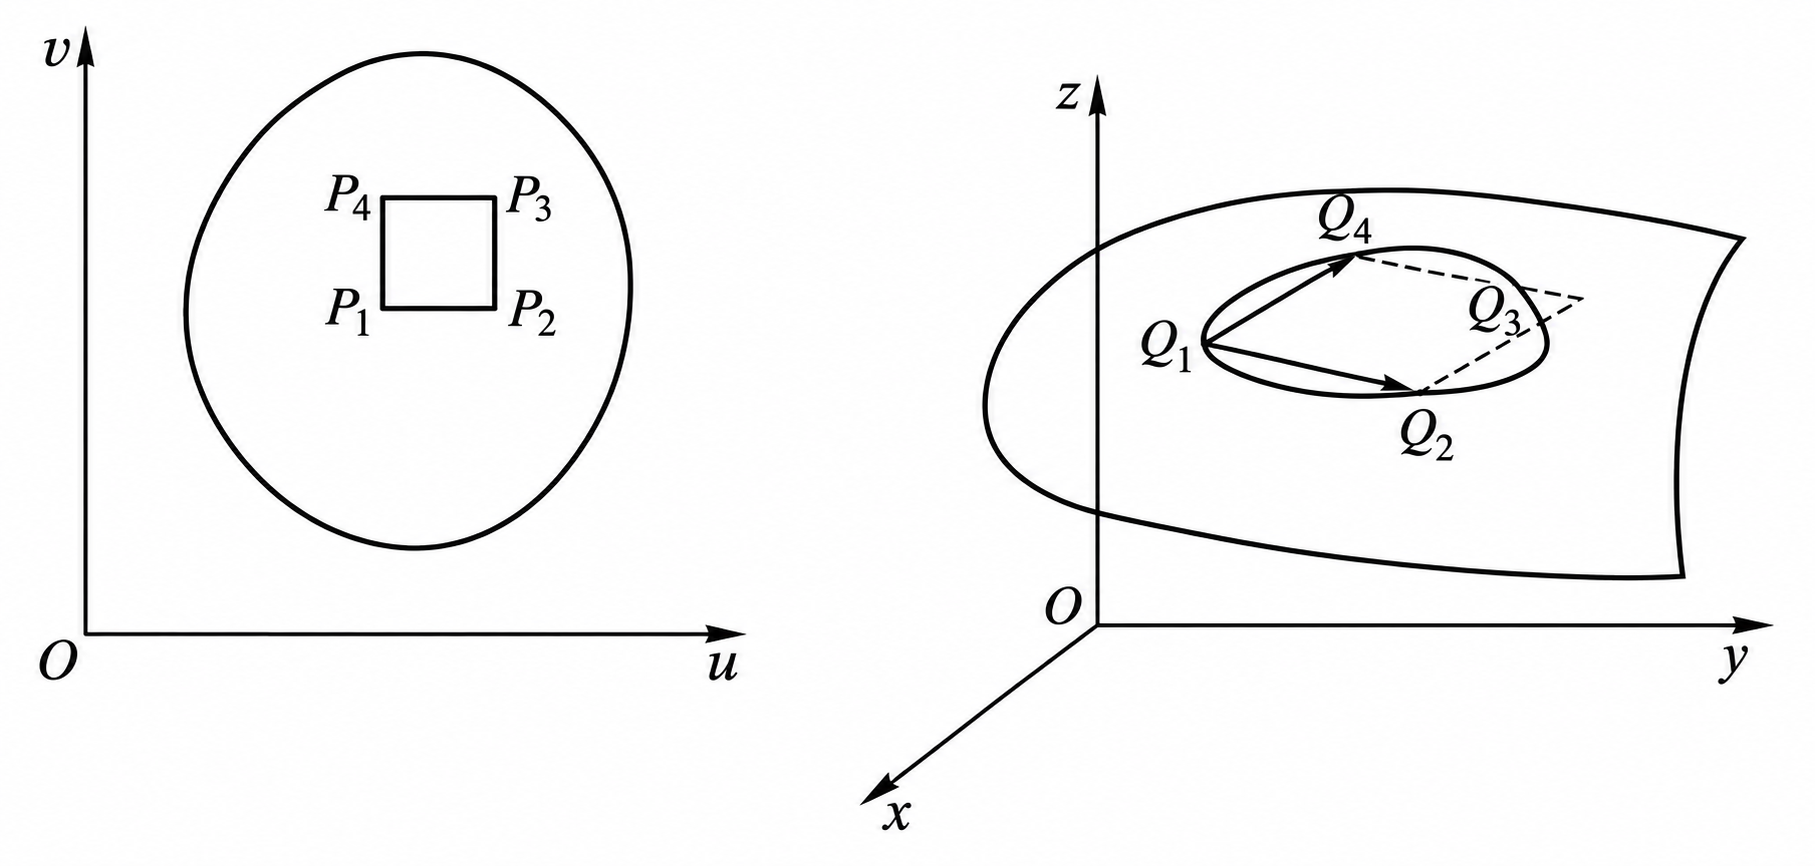
\includegraphics[width=0.78\linewidth]{figure/P2/fig14_1_3_redrawn_hd.png}
\end{center}
由中值定理，
\[
\begin{aligned}
\overrightarrow{Q_1Q_2}
&=\boldsymbol r(u_0+\Delta u,v_0)-\boldsymbol r(u_0,v_0)
=\boldsymbol r_u(u_0,v_0)\Delta u+o(\Delta u),\\
\overrightarrow{Q_1Q_4}
&=\boldsymbol r(u_0,v_0+\Delta v)-\boldsymbol r(u_0,v_0)
=\boldsymbol r_v(u_0,v_0)\Delta v+o(\Delta v).
\end{aligned}
\]
这里 $o(\Delta u),o(\Delta v)$ 表示模分别为 $\Delta u,\Delta v$ 的高阶无穷小的向量。小曲面片的面积可近似为切平面上以 $\boldsymbol r_u\Delta u$ 和 $\boldsymbol r_v\Delta v$ 为邻边的平行四边形的面积。因此曲面的面积微元和面积分别为
\[
\dd S=\lVert\boldsymbol r_u\times\boldsymbol r_v\rVert\,\dd u\dd v,\qquad
S=\displaystyle\iint_D\lVert\boldsymbol r_u\times\boldsymbol r_v\rVert\,\dd u\dd v.
\]
利用面积的可加性，这一方法可推广到由有限片这样的曲面拼成的分片光滑曲面。

\begin{theorem}
对上述曲面 $\Sigma$，记 Gauss 系数
\[
\begin{aligned}
E&=\boldsymbol r_u\cdot\boldsymbol r_u=x_u^2+y_u^2+z_u^2,\\
F&=\boldsymbol r_u\cdot\boldsymbol r_v=x_ux_v+y_uy_v+z_uz_v,\\
G&=\boldsymbol r_v\cdot\boldsymbol r_v=x_v^2+y_v^2+z_v^2.
\end{aligned}
\]
则曲面面积为
\[
S=\displaystyle\iint_D\sqrt{EG-F^2}\,\dd u\dd v.
\]
\end{theorem}
\begin{proof}
由外积的坐标表达式，
\[
\boldsymbol r_u\times\boldsymbol r_v
=\frac{\partial(y,z)}{\partial(u,v)}\boldsymbol i
+\frac{\partial(z,x)}{\partial(u,v)}\boldsymbol j
+\frac{\partial(x,y)}{\partial(u,v)}\boldsymbol k.
\]
因此
\[
\lVert\boldsymbol r_u\times\boldsymbol r_v\rVert^2
=\left(\frac{\partial(y,z)}{\partial(u,v)}\right)^2
+\left(\frac{\partial(z,x)}{\partial(u,v)}\right)^2
+\left(\frac{\partial(x,y)}{\partial(u,v)}\right)^2.
\]
将 $E,G,F$ 的表达式展开并合并同类项，得到同样的平方和，即
\[
EG-F^2=\lVert\boldsymbol r_u\times\boldsymbol r_v\rVert^2.
\]
代入曲面面积公式，即得结论。
\end{proof}

\begin{enumerate}
\item 若曲面方程为 $z=f(x,y)$，$(x,y)\in D$，其中 $f$ 具有连续偏导数，$D$ 是具有分段光滑边界的有界区域，则
\[
\boldsymbol r=x\boldsymbol i+y\boldsymbol j+f(x,y)\boldsymbol k,
\quad \boldsymbol r_x=\boldsymbol i+f_x\boldsymbol k,
\quad \boldsymbol r_y=\boldsymbol j+f_y\boldsymbol k.
\]
由 $EG-F^2=(1+f_x^2)(1+f_y^2)-f_x^2f_y^2=1+f_x^2+f_y^2$，得
\[
S=\displaystyle\iint_D\sqrt{1+f_x^2+f_y^2}\,\dd x\dd y.
\]
\item 若曲面方程为 $H(x,y,z)=0$，其中 $H$ 具有连续偏导数，且在曲面上 $H_z\ne0$；又设曲面在 $xy$ 平面上的投影将曲面一一对应地映为具有分段光滑边界的有界区域 $D$。由隐函数定理，曲面可表示为 $z=f(x,y)$，且
\[
f_x=-\frac{H_x}{H_z},\qquad f_y=-\frac{H_y}{H_z}.
\]
因此
\[
\begin{aligned}
S&=\displaystyle\iint_D\sqrt{1+\left(\frac{H_x}{H_z}\right)^2+\left(\frac{H_y}{H_z}\right)^2}\,\dd x\dd y\\
&=\displaystyle\iint_D\frac{\lVert\operatorname{grad}H\rVert}{|H_z|}\,\dd x\dd y.
\end{aligned}
\]
\end{enumerate}



\subsection*{Schwarz 的例子}
光滑曲线的弧长可以用内接折线长度的极限定义，但这一方法不能直接推广到曲面的面积：即使内接多面体各个三角形的直径都趋于零，其面积和也未必趋于曲面的面积。

设圆柱面的高为 $h>0$，半径为 $r>0$，其侧面积为 $2\pi rh$。在圆柱面上取三点 $A,B,C$，使 $A,B$ 在同一高度，$C$ 在另一高度，且 $C$ 在 $A,B$ 所在水平面上的投影 $C'$ 是短圆弧 $AB$ 的中点。连接 $A,B,C$，得到一个内接三角形。

将底圆 $m$ 等分，高 $n$ 等分；在各个水平截圆上取 $m$ 个等分点，相邻两层的等分点沿圆周错开半个分度，再连接相邻层的点，组成内接多面体的侧面。这样共有 $2mn$ 个全等三角形。
\begin{center}
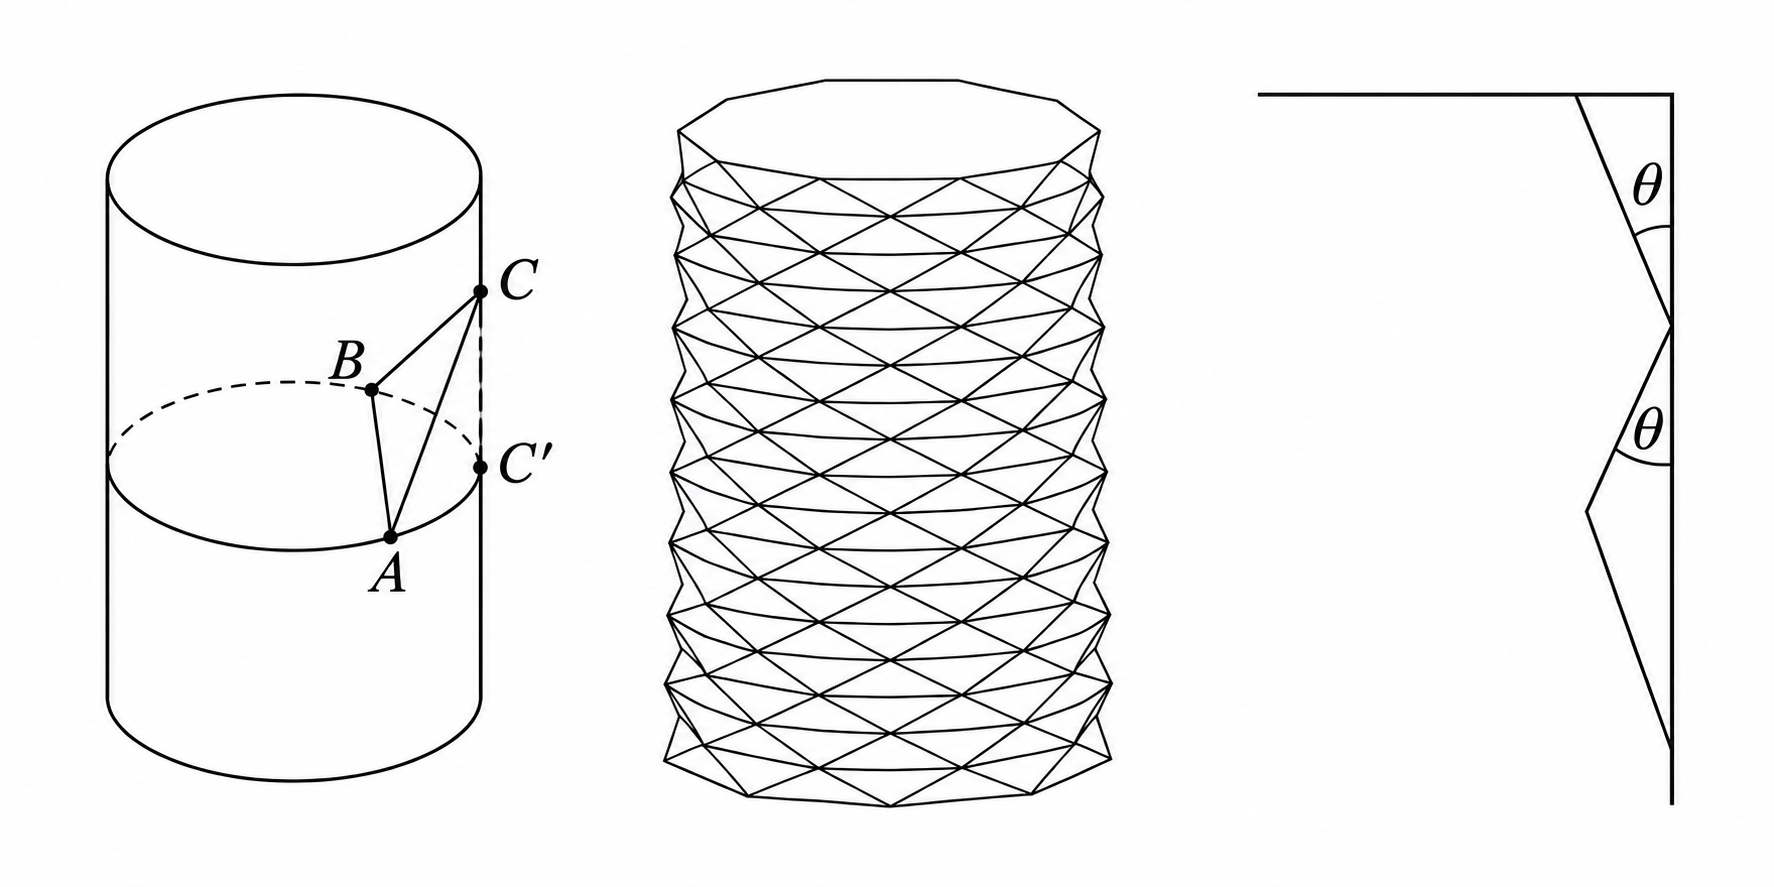
\includegraphics[width=0.95\linewidth]{figure/P2/schwarz_lantern_redrawn_hd.png}
\end{center}
每个三角形中，平行于底圆平面的底边长为
\[
b_m=2r\sin\frac{\pi}{m}.
\]
记底边中点为 $M$。由 $C'$ 是短圆弧 $AB$ 的中点，$C'M$ 垂直于弦 $AB$，且
\[
C'M=r\left(1-\cos\frac{\pi}{m}\right),\qquad CC'=\frac hn.
\]
又 $CC'$ 垂直于底圆平面，所以 $CM$ 是三角形 $ABC$ 的高，其长度为
\[
a_{m,n}=\sqrt{r^2\left(1-\cos\frac{\pi}{m}\right)^2+\frac{h^2}{n^2}}.
\]
由 $1-\cos t=2\sin^2(t/2)$，每个三角形的面积为
\[
\frac12 b_ma_{m,n}
=r\sin\frac{\pi}{m}\sqrt{4r^2\sin^4\frac{\pi}{2m}+\frac{h^2}{n^2}}.
\]
于是所有小三角形的面积之和为
\begin{align*}
S_{m,n}
&=2mnr\sin\frac{\pi}{m}\sqrt{4r^2\sin^4\frac{\pi}{2m}+\frac{h^2}{n^2}}\\
&=2\pi rh\frac{\sin(\pi/m)}{\pi/m}
\sqrt{1+\frac{\pi^4r^2}{4h^2}
\left(\frac{\sin(\pi/(2m))}{\pi/(2m)}\right)^4\frac{n^2}{m^4}}.
\end{align*}
当 $m,n\to\infty$ 时，各个三角形的直径确实趋于零：其底边长趋于零，另外两条边的长度均为
\[
\sqrt{4r^2\sin^2\frac{\pi}{2m}+\frac{h^2}{n^2}}\longrightarrow0.
\]
但面积和的极限取决于 $n/m^2$。若
\[
\frac{n}{m^2}\longrightarrow l\in[0,+\infty),
\]
则由 $\sin t/t\to1$，得到
\[
S_{m,n}\longrightarrow S(l)
=2\pi r\sqrt{h^2+\frac{\pi^4r^2l^2}{4}}.
\]
只有当 $l=0$ 时，这个极限才是圆柱面的侧面积 $2\pi rh$。例如，取 $n=m$ 时极限为 $2\pi rh$；取 $n=m^2$ 时极限严格大于 $2\pi rh$。若 $n/m^2\to+\infty$，则面积和趋于 $+\infty$。

因此，$m,n$ 同时趋于无穷的方式不同，面积和可以有不同的极限；仅要求小三角形的最大直径趋于零，不能用内接多面体面积的极限定义曲面面积。

再考察 $l=0$ 的几何意义。设 $\theta$ 为三角形所在平面与圆柱面在 $C'$ 处的母线的夹角。由于 $AB$ 垂直于由 $CC'$ 和 $C'M$ 张成的平面，在该截面内计算可得
\begin{align*}
\tan\theta
&=\frac{r-r\cos(\pi/m)}{h/n}
=\frac{2r\sin^2(\pi/(2m))}{h/n}\\
&=\frac{\pi^2r}{2h}
\left(\frac{\sin(\pi/(2m))}{\pi/(2m)}\right)^2\frac{n}{m^2}.
\end{align*}
所以，当 $n/m^2\to0$ 时，$\theta\to0$。在这一构造中，三角形平面含有与该处圆周切线平行的方向；因此 $\theta\to0$ 也表示三角形所在平面趋于相应的切平面。这与前面用切平面上的平行四边形计算面积微元的讨论相吻合。


\subsection*{第一类曲面积分}
\begin{definition}
设 $\Sigma$ 为有界光滑或分片光滑曲面，$f(x,y,z)$ 在 $\Sigma$ 上有界。用光滑曲线网将 $\Sigma$ 分成 $n$ 片小曲面 $\Delta\Sigma_1,\ldots,\Delta\Sigma_n$，记第 $i$ 片的面积为 $\Delta S_i$，并在其上任取一点 $(\xi_i,\eta_i,\zeta_i)$，作和式
\[
\sum_{i=1}^n f(\xi_i,\eta_i,\zeta_i)\Delta S_i.
\]
如果当所有小曲面直径的最大值 $\lambda\to0$ 时，这个和式的极限存在，且与划分及取点无关，就称该极限为 $f$ 在 $\Sigma$ 上的第一类曲面积分，记为
\[
\displaystyle\iint_\Sigma f(x,y,z)\,\dd S
=\lim_{\lambda\to0}\sum_{i=1}^n f(\xi_i,\eta_i,\zeta_i)\Delta S_i.
\]
其中 $f$ 称为被积函数，$\Sigma$ 称为积分曲面。
\end{definition}

设 $\Sigma$ 具有上面的参数表示，参数映射一一对应且满足前述光滑条件。如果 $f$ 在 $\Sigma$ 上连续，则第一类曲面积分存在，且
\[
\displaystyle\iint_\Sigma f(x,y,z)\,\dd S
=\displaystyle\iint_D f(x(u,v),y(u,v),z(u,v))\sqrt{EG-F^2}\,\dd u\dd v.
\]
特别地，若 $\Sigma$ 的方程为 $z=z(x,y)$，$(x,y)\in D$，则
\[
\displaystyle\iint_\Sigma f(x,y,z)\,\dd S
=\displaystyle\iint_D f(x,y,z(x,y))\sqrt{1+z_x^2+z_y^2}\,\dd x\dd y.
\]

% 原图未给出曲面积分计算公式的证明。
\begin{proof}
记 $g(u,v)=f(\boldsymbol r(u,v))$，$w(u,v)=\lVert\boldsymbol r_u\times\boldsymbol r_v\rVert$。对曲面的小片划分，记 $D_i$ 为 $\Delta\Sigma_i$ 在参数区域中的原像，并取 $p_i\in D_i$ 对应所选的曲面上的点。由曲面面积公式，
\[
\Delta S_i=\displaystyle\iint_{D_i}w(u,v)\,\dd u\dd v.
\]
于是相应的曲面积分和与右端积分之差为
\[
\sum_i f(\boldsymbol r(p_i))\Delta S_i
-\displaystyle\iint_D gw\,\dd u\dd v
=\sum_i\displaystyle\iint_{D_i}[g(p_i)-g(u,v)]w(u,v)\,\dd u\dd v.
\]
由于 $D$ 是紧集，连续单射 $\boldsymbol r:D\to\Sigma$ 的逆映射连续且一致连续。当曲面小片的最大直径趋于零时，各 $D_i$ 的直径也一致趋于零。又 $g$ 在 $D$ 上一致连续，所以
\[
\max_i\sup_{(u,v)\in D_i}|g(p_i)-g(u,v)|\longrightarrow0.
\]
上面差式的绝对值因此不超过这个最大值与曲面面积
$\displaystyle\iint_Dw\,\dd u\dd v$ 的乘积，故趋于零。这就证明了积分的存在性及计算公式。将 $\boldsymbol r(x,y)=(x,y,z(x,y))$ 代入即可得到特殊情形。
\end{proof}
%

% 第2节：第二类曲线积分与曲面积分
%% !TEX root = ../../../main.tex
% 第二部分第四章第二节：第二类曲线积分与曲面积分
\section{第二类曲线积分与曲面积分}
\subsection*{第二类曲线积分}
设空间力场为
\[
\boldsymbol F(x,y,z)=P(x,y,z)\boldsymbol i+Q(x,y,z)\boldsymbol j+R(x,y,z)\boldsymbol k.
\]
物体沿有向曲线 $L$ 从 $A$ 运动到 $B$，力场所做的功可由下面的积分表示。
\begin{definition}
设 $L$ 为有向光滑曲线，$\boldsymbol F$ 在 $L$ 上有界。沿指定方向取分点 $A=P_0,P_1,\ldots,P_n=B$。记小弧段 $\wideparen{P_{k-1}P_k}$ 的长度为 $\Delta s_k$，在其上任取一点 $X_k=(\xi_k,\eta_k,\zeta_k)$，以 $\boldsymbol\tau(X_k)$ 表示该点沿曲线指定方向的单位切向量。小弧段上的功近似为
\[
\Delta W_k\approx\boldsymbol F(X_k)\cdot\boldsymbol\tau(X_k)\Delta s_k.
\]
作和式
\[
S_n=\sum_{k=1}^n\boldsymbol F(X_k)\cdot\boldsymbol\tau(X_k)\Delta s_k,
\qquad \lambda=\max_k\Delta s_k.
\]
若 $\lambda\to0$ 时该和式有有限极限，且与划分及取点无关，则称其为 $\boldsymbol F$ 沿 $L$ 的第二类曲线积分，记为
\[
I=\int_L\boldsymbol F\cdot\boldsymbol\tau\,\dd s
=\lim_{\lambda\to0}S_n.
\]
记 $\dd\boldsymbol s=\boldsymbol\tau\,\dd s$，也写作 $\displaystyle\int_L\boldsymbol F\cdot\dd\boldsymbol s$。
\end{definition}
若单位切向量与三个坐标轴的夹角为 $\alpha,\beta,\gamma$，则
\[
\boldsymbol\tau=\cos\alpha\,\boldsymbol i+\cos\beta\,\boldsymbol j+\cos\gamma\,\boldsymbol k,
\]
从而第二类曲线积分化为第一类曲线积分：
\[
I=\int_L(P\cos\alpha+Q\cos\beta+R\cos\gamma)\,\dd s.
\]
沿曲线有 $\dd x=\cos\alpha\,\dd s$、$\dd y=\cos\beta\,\dd s$、$\dd z=\cos\gamma\,\dd s$，因此又记为
\[
I=\int_LP\,\dd x+Q\,\dd y+R\,\dd z.
\]
特别地，若 $L$ 是 $xy$ 平面上的有向光滑曲线，则
\begin{align*}
\int_LP\,\dd x+Q\,\dd y
&=\int_L(P\cos\alpha+Q\cos\beta)\,\dd s\\
&=\int_L(P\cos\alpha+Q\sin\alpha)\,\dd s.
\end{align*}
这里平面情形的 $\alpha$ 是有向切向量与 $x$ 轴正向所成的有向角。

\begin{proposition}
\begin{enumerate}
\item 方向性：记 $-L$ 为 $L$ 的反向曲线，则
\[
\int_{-L}\boldsymbol F\cdot\boldsymbol\tau\,\dd s
=-\int_L\boldsymbol F\cdot\boldsymbol\tau\,\dd s.
\]
\item 线性性：若 $\boldsymbol F,\boldsymbol G$ 沿 $L$ 可积，$a,b$ 为常数，则
\[
\int_L(a\boldsymbol F+b\boldsymbol G)\cdot\boldsymbol\tau\,\dd s
=a\int_L\boldsymbol F\cdot\boldsymbol\tau\,\dd s+b\int_L\boldsymbol G\cdot\boldsymbol\tau\,\dd s.
\]
\item 路径可加性：若有向曲线 $L=L_1+L_2$ 由方向相容的两段拼成，则沿 $L$ 可积当且仅当沿两段均可积，且
\[
\int_L\boldsymbol F\cdot\boldsymbol\tau\,\dd s
=\int_{L_1}\boldsymbol F\cdot\boldsymbol\tau\,\dd s+\int_{L_2}\boldsymbol F\cdot\boldsymbol\tau\,\dd s.
\]
\end{enumerate}
\end{proposition}
% 原图未展开这三条性质的证明。
\begin{proof}
\begin{enumerate}
\item 反向后单位切向量变为 $-\boldsymbol\tau$，弧长微元不变，故每个对应积分和变号，取极限即得结论。
\item 每个积分和关于被积向量场都是线性的，将和式拆开并分别取极限，便得到所述等式。
\item 在拼接点处分开划分，积分和即分成两段上的积分和。反之，把标量函数 $\boldsymbol F\cdot\boldsymbol\tau$ 看作第一类曲线积分的被积函数，利用其路径可加性及可积性的限制性质，得到可积性的等价关系与等式。分段光滑曲线的有限个拼接点不影响积分值。
\end{enumerate}
\end{proof}

\begin{theorem}
设 $L$ 的光滑参数表示为
\[
x=x(t),\quad y=y(t),\quad z=z(t),\qquad a\le t\le b,
\]
参数从 $a$ 增至 $b$ 时与 $L$ 的方向一致，且 $P,Q,R$ 在 $L$ 上连续，则
\begin{align*}
\int_LP\,\dd x+Q\,\dd y+R\,\dd z
=\int_a^b\bigl[&P(x(t),y(t),z(t))x'(t)\\
&+Q(x(t),y(t),z(t))y'(t)\\
&+R(x(t),y(t),z(t))z'(t)\bigr]\,\dd t.
\end{align*}
\end{theorem}
\begin{proof}
记 $\boldsymbol r(t)=(x(t),y(t),z(t))$ 及 $v(t)=\lVert\boldsymbol r'(t)\rVert>0$，则
\[
\boldsymbol\tau(\boldsymbol r(t))=\frac{\boldsymbol r'(t)}{v(t)},
\qquad \dd s=v(t)\,\dd t.
\]
对参数划分 $a=t_0<\cdots<t_n=b$，在对应弧段上取点 $\boldsymbol r(\bar t_k)$。由积分中值定理，可取 $\theta_k\in[t_{k-1},t_k]$ 使
\[
\Delta s_k=v(\theta_k)\Delta t_k.
\]
因此
\[
S_n=\sum_{k=1}^n
\boldsymbol F(\boldsymbol r(\bar t_k))\cdot
\frac{\boldsymbol r'(\bar t_k)}{v(\bar t_k)}
v(\theta_k)\Delta t_k.
\]
由于 $v$ 连续且在闭区间上有正的下界，弧长划分模长趋于零时，参数划分模长也趋于零；由一致连续性，$v(\theta_k)/v(\bar t_k)\to1$ 一致成立。于是上式与
\[
\sum_{k=1}^n\boldsymbol F(\boldsymbol r(\bar t_k))\cdot\boldsymbol r'(\bar t_k)\Delta t_k
\]
之差趋于零。后者是连续函数 $\boldsymbol F(\boldsymbol r(t))\cdot\boldsymbol r'(t)$ 的 Riemann 和，其极限即为所述积分。
\end{proof}

特别地，若空间曲线以 $x$ 为参数，方程为 $y=y(x),z=z(x)$，方向为 $x:a\to b$，则
\[
\begin{aligned}
\int_LP\,\dd x+Q\,\dd y+R\,\dd z
=\int_a^b\bigl[&P(x,y(x),z(x))\\
&+Q(x,y(x),z(x))y'(x)\\
&+R(x,y(x),z(x))z'(x)\bigr]\,\dd x.
\end{aligned}
\]
对于平面有向光滑曲线 $x=x(t),y=y(t)$，有
\[
\int_LP\,\dd x+Q\,\dd y
=\int_a^b[P(x(t),y(t))x'(t)+Q(x(t),y(t))y'(t)]\,\dd t.
\]
若平面曲线方程为 $y=y(x)$，方向为 $x:a\to b$，则
\[
\int_LP\,\dd x+Q\,\dd y
=\int_a^b[P(x,y(x))+Q(x,y(x))y'(x)]\,\dd x.
\]

\subsection*{曲面的侧}
\begin{definition}
设 $\Sigma$ 为光滑曲面，$P\in\Sigma$。从 $P$ 出发沿曲面上不经过边界的任一简单闭曲线连续移动一个单位法向量，回到 $P$ 时，若其方向总与出发时一致，则称 $\Sigma$ 为双侧曲面。
\end{definition}
在双侧曲面上选定一点的一个单位法向量，并连续地移动该法向量，就确定了曲面的一侧。两种相反的连续单位法向量场给出曲面的两侧，选定一侧的曲面称为定向曲面。

并非所有光滑曲面都是双侧曲面。例如，将长方形纸片 $ABCD$ 的一端扭转半周，使 $A$ 与 $C$、$B$ 与 $D$ 重合后粘接，得到 M\"obius 带。从一点出发沿带连续移动单位法向量，绕行一周回到原点时，法向量反向，因此它是单侧曲面。
\begin{center}
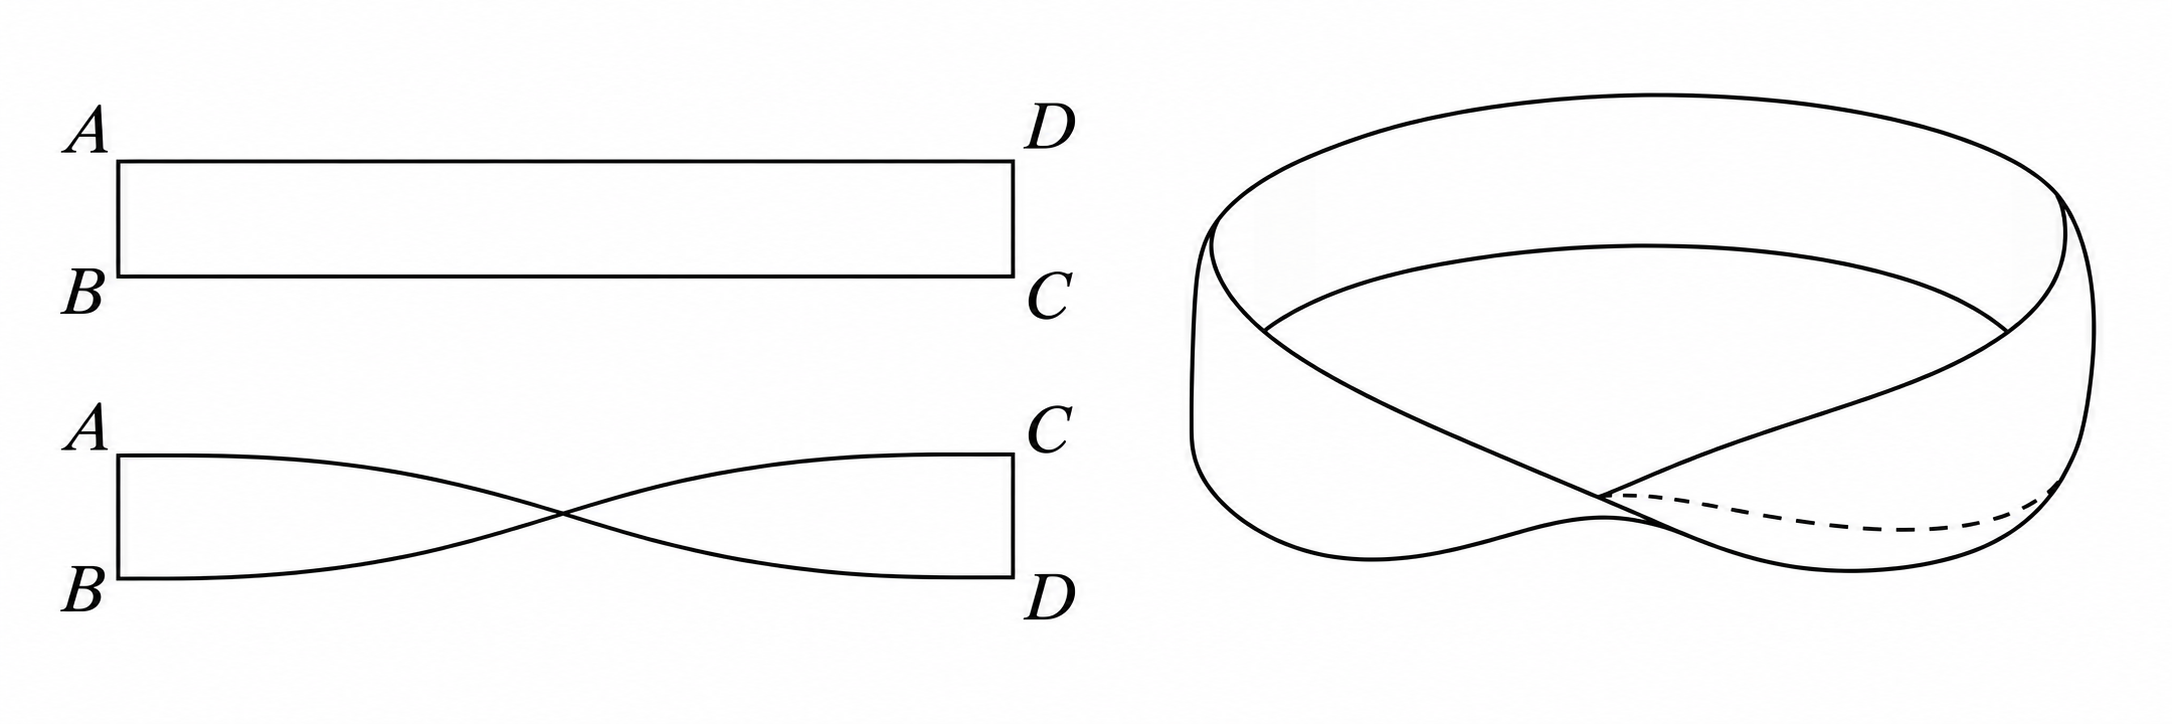
\includegraphics[width=0.92\linewidth]{figure/P2/mobius_redrawn_hd.png}
\end{center}
以下只讨论双侧曲面。注意，双侧曲面拼接后未必仍是双侧曲面；例如 M\"obius 带可以由两片双侧曲面拼接而成。

\subsection*{第二类曲面积分}
设曲面有参数表示
\[
x=x(u,v),\quad y=y(u,v),\quad z=z(u,v),\qquad (u,v)\in D,
\]
其中参数函数具有连续偏导数，记
\[
\boldsymbol r(u,v)=x(u,v)\boldsymbol i+y(u,v)\boldsymbol j+z(u,v)\boldsymbol k.
\]
在正则点，$\boldsymbol r_u\times\boldsymbol r_v\ne\boldsymbol0$。该向量同时垂直于两条参数曲线的切向量，给出曲面的一个法向方向。因而两种法向量可表示为
\[
\pm\boldsymbol r_u\times\boldsymbol r_v
=\pm\left(\frac{\partial(y,z)}{\partial(u,v)},
\frac{\partial(z,x)}{\partial(u,v)},
\frac{\partial(x,y)}{\partial(u,v)}\right).
\]
相应的单位法向量为
\[
\begin{aligned}
\boldsymbol n&=(\cos\alpha,\cos\beta,\cos\gamma)\\
&=\frac{\pm1}{\sqrt{EG-F^2}}
\left(\frac{\partial(y,z)}{\partial(u,v)},
\frac{\partial(z,x)}{\partial(u,v)},
\frac{\partial(x,y)}{\partial(u,v)}\right),
\end{aligned}
\]
其中
\[
EG-F^2=
\left(\frac{\partial(y,z)}{\partial(u,v)}\right)^2+
\left(\frac{\partial(z,x)}{\partial(u,v)}\right)^2+
\left(\frac{\partial(x,y)}{\partial(u,v)}\right)^2.
\]
对于这一正则参数表示，选定正负号便给出每一点的单位法向量。由于偏导数连续，所取单位法向量随点连续变化；在双侧曲面上使各参数片的法向选择相容，就确定了曲面的一侧。

% 以下按新提供图片的左栏、右栏顺序续写。
\subsection*{法向的选择}
以下以向上的一侧为例；对封闭曲面，则需按题意判断取外侧还是内侧。不能对整个球面都取向上的法向量，否则会在赤道处发生矛盾。例如，球面取外侧时，上半球的法向量指向上方，下半球的法向量指向下方。

对于由四个三角形面组成的四面体表面，也应分别判断各面的外侧，再使各面的取向与整体的外侧相容。
\begin{center}
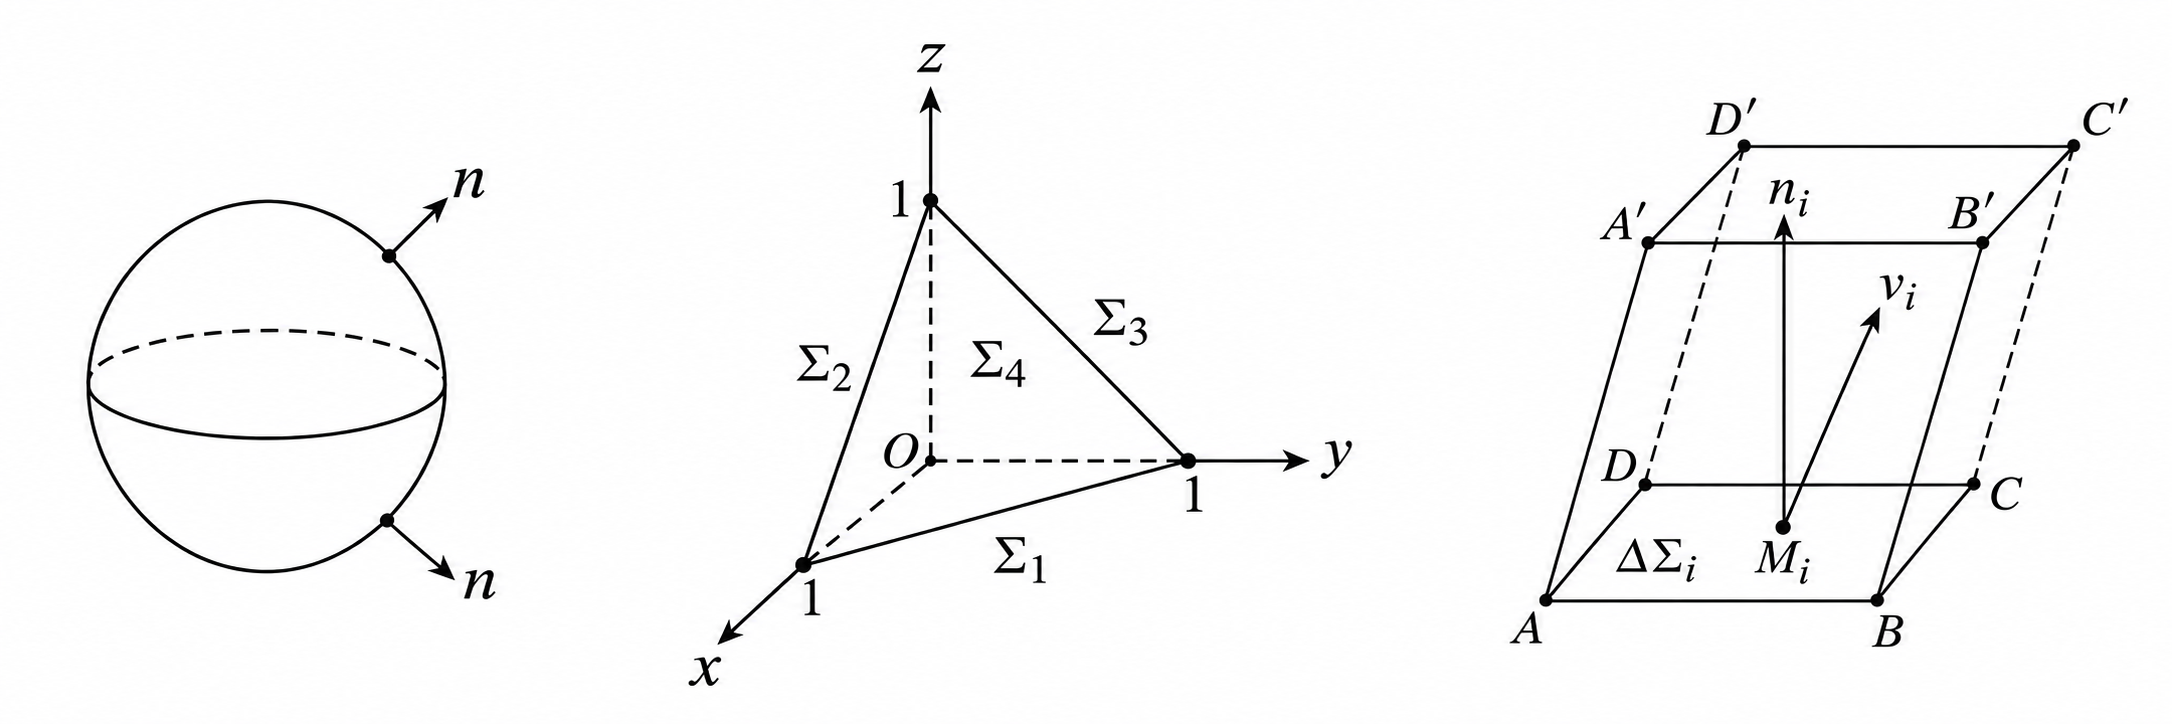
\includegraphics[width=0.98\linewidth]{figure/P2/flux_orientation_redrawn_hd.png}
\end{center}
若所取一侧的法向量的第三个分量为正，则比较
\[
(\boldsymbol r_u\times\boldsymbol r_v)_3
=\frac{\partial(x,y)}{\partial(u,v)}
=\begin{vmatrix}x_u&y_u\\x_v&y_v\end{vmatrix}.
\]
当这个行列式大于零时，取 $+\boldsymbol r_u\times\boldsymbol r_v$；小于零时，取 $-\boldsymbol r_u\times\boldsymbol r_v$。若该分量为零，就须通过其他非零分量判断，不能仅用第三个分量选定方向。

\subsection*{通量与第二类曲面积分的定义}
设有不可压缩流体，密度为 $1$，速度场为
\[
\boldsymbol v(x,y,z)=P(x,y,z)\boldsymbol i+Q(x,y,z)\boldsymbol j+R(x,y,z)\boldsymbol k.
\]
求单位时间内通过定向曲面 $\Sigma$ 的流量。用光滑曲线网将 $\Sigma$ 分成小曲面 $\Delta\Sigma_i$，其面积为 $\Delta S_i$。在每片上取点 $M_i=(\xi_i,\eta_i,\zeta_i)$，记该点的速度为 $\boldsymbol v_i$，所选一侧的单位法向量为
\[
\boldsymbol n_i=\cos\alpha_i\,\boldsymbol i+\cos\beta_i\,\boldsymbol j+\cos\gamma_i\,\boldsymbol k.
\]
在短时间 $\Delta t$ 内，流经小曲面片的体积近似为以该片为底、以 $\boldsymbol v_i\Delta t$ 为侧棱的斜柱体体积，其有向值为
\[
(\boldsymbol v_i\cdot\boldsymbol n_i)\Delta S_i\Delta t.
\]
除以 $\Delta t$，相加并令所有小片的最大直径 $\lambda$ 趋于零，得到单位时间内的总流量
\begin{align*}
\Phi
&=\lim_{\lambda\to0}\sum_i\boldsymbol v_i\cdot\boldsymbol n_i\Delta S_i\\
&=\displaystyle\iint_\Sigma(P\cos\alpha+Q\cos\beta+R\cos\gamma)\,\dd S.
\end{align*}
这里正值表示沿所选法向流出，负值表示反向流入。

\begin{definition}
设 $\Sigma$ 为定向光滑曲面，所选一侧的单位法向量为 $\boldsymbol n=(\cos\alpha,\cos\beta,\cos\gamma)$，向量场 $\boldsymbol F=(P,Q,R)$ 定义在 $\Sigma$ 上。称
\[
\displaystyle\iint_\Sigma\boldsymbol F\cdot\boldsymbol n\,\dd S
=\displaystyle\iint_\Sigma(P\cos\alpha+Q\cos\beta+R\cos\gamma)\,\dd S
\]
为 $\boldsymbol F$ 在 $\Sigma$ 上的第二类曲面积分，只要右端的第一类曲面积分存在。
\end{definition}
记 $\dd\boldsymbol S=\boldsymbol n\,\dd S$，也称为有向面积元，于是积分可记为 $\displaystyle\iint_\Sigma\boldsymbol F\cdot\dd\boldsymbol S$。并记
\[
\dd y\dd z=\cos\alpha\,\dd S,\qquad
\dd z\dd x=\cos\beta\,\dd S,\qquad
\dd x\dd y=\cos\gamma\,\dd S,
\]
则有
\[
\displaystyle\iint_\Sigma\boldsymbol F\cdot\boldsymbol n\,\dd S
=\displaystyle\iint_\Sigma P\,\dd y\wedge\dd z+Q\,\dd z\wedge\dd x+R\,\dd x\wedge\dd y.
\]
\[\dd y\wedge\dd z= \dd y\dd z,\quad   \dd z\wedge\dd x= \dd z\dd x,\quad  \dd x\wedge\dd y=\dd x\dd y\]
这里的 $\dd y\dd z,\dd z\dd x,\dd x\dd y$ 表示带方向的投影面积元，顺序与方向有关，不能当作普通的无向面积元任意交换次序。

\subsection*{计算公式}
对于正则参数表示 $\boldsymbol r(u,v)$，先按所选一侧确定符号 $\varepsilon\in\{1,-1\}$，使
\[
\boldsymbol n=\varepsilon\frac{\boldsymbol r_u\times\boldsymbol r_v}{\lVert\boldsymbol r_u\times\boldsymbol r_v\rVert}.
\]
由 $\dd S=\lVert\boldsymbol r_u\times\boldsymbol r_v\rVert\,\dd u\dd v$，得到
\begin{align*}
I&=\varepsilon\displaystyle\iint_D
\begin{vmatrix}P&Q&R\\x_u&y_u&z_u\\x_v&y_v&z_v\end{vmatrix}\,\dd u\dd v\\
&=\varepsilon\displaystyle\iint_D\left[
P\frac{\partial(y,z)}{\partial(u,v)}+
Q\frac{\partial(z,x)}{\partial(u,v)}+
R\frac{\partial(x,y)}{\partial(u,v)}\right]\,\dd u\dd v.
\end{align*}
其中 $P,Q,R$ 都在 $(x(u,v),y(u,v),z(u,v))$ 处取值。这同时给出了第二类曲面积分化为参数区域上二重积分的公式。

\begin{proposition}
\begin{enumerate}
\item 方向性：若 $-\Sigma$ 表示与 $\Sigma$ 取向相反的曲面，则
\[
\displaystyle\iint_{-\Sigma}\boldsymbol F\cdot\boldsymbol n\,\dd S
=-\displaystyle\iint_\Sigma\boldsymbol F\cdot\boldsymbol n\,\dd S.
\]
\item 线性性：若 $\boldsymbol F,\boldsymbol G$ 在 $\Sigma$ 上可积，$a,b$ 为常数，则
\[
\displaystyle\iint_\Sigma(a\boldsymbol F+b\boldsymbol G)\cdot\boldsymbol n\,\dd S
=a\displaystyle\iint_\Sigma\boldsymbol F\cdot\boldsymbol n\,\dd S
+b\displaystyle\iint_\Sigma\boldsymbol G\cdot\boldsymbol n\,\dd S.
\]
\item 曲面可加性：若 $\Sigma=\Sigma_1+\Sigma_2$，两片取向与整体一致且仅沿边界相接，则在 $\Sigma$ 上可积当且仅当在两片上均可积，并有
\[
\displaystyle\iint_\Sigma\boldsymbol F\cdot\boldsymbol n\,\dd S
=\displaystyle\iint_{\Sigma_1}\boldsymbol F\cdot\boldsymbol n\,\dd S
+\displaystyle\iint_{\Sigma_2}\boldsymbol F\cdot\boldsymbol n\,\dd S.
\]
\end{enumerate}
\end{proposition}
% 原图未展开三条性质的证明。
\begin{proof}
\begin{enumerate}
\item 取向反转使 $\boldsymbol n$ 变为 $-\boldsymbol n$，而无向面积元 $\dd S$ 不变，所以积分变号。
\item 将 $(a\boldsymbol F+b\boldsymbol G)\cdot\boldsymbol n$ 展开为 $a(\boldsymbol F\cdot\boldsymbol n)+b(\boldsymbol G\cdot\boldsymbol n)$，再用第一类曲面积分的线性性即得结论。
\item 将标量被积函数写为 $\boldsymbol F\cdot\boldsymbol n$，按两片曲面分别划分，积分和分成对应的两个和式。沿共同边界的光滑曲线面积为零，不影响积分；因此第一类曲面积分的可加性给出可积性的等价关系及所述等式。
\end{enumerate}
\end{proof}

\begin{example}
设 $\Sigma$ 是由坐标平面和 $x+y+z=1$ 围成的第一卦限内四面体的表面，取外侧，求
\[
I=\displaystyle\iint_\Sigma(x+1)\,\dd y\dd z+(y+1)\,\dd z\dd x+(z+1)\,\dd x\dd y.
\]
\end{example}
\begin{solution}
依次记 $z=0,y=0,x=0,x+y+z=1$ 上的四个面为 $\Sigma_1,\Sigma_2,\Sigma_3,\Sigma_4$，各取四面体外侧。记每个面上的积分为 $I_j$，则 $I=I_1+I_2+I_3+I_4$。

对于 $\Sigma_1$，取 $\boldsymbol r(x,y)=(x,y,0)$，参数域
\[
D_1=\{(x,y):x\ge0,\ y\ge0,\ x+y\le1\}.
\]
此时 $\boldsymbol r_x\times\boldsymbol r_y=(0,0,1)$，但外侧向下，须取负号。因此
\[
I_1=-\displaystyle\iint_{D_1}
\begin{vmatrix}x+1&y+1&1\\1&0&0\\0&1&0\end{vmatrix}\,\dd x\dd y
=-\displaystyle\iint_{D_1}1\,\dd x\dd y=-\frac12.
\]
对于 $\Sigma_2$，取 $\boldsymbol r(x,z)=(x,0,z)$，参数域 $D_2=\{(x,z):x,z\ge0,\ x+z\le1\}$。因为
\[
\boldsymbol r_x\times\boldsymbol r_z=(0,-1,0),
\]
它已经指向外侧，故取正号：
\[
I_2=\displaystyle\iint_{D_2}
\begin{vmatrix}x+1&1&z+1\\1&0&0\\0&0&1\end{vmatrix}\,\dd x\dd z
=-\displaystyle\iint_{D_2}1\,\dd x\dd z=-\frac12.
\]
同样，$\Sigma_3$ 的外法向量为 $(-1,0,0)$，其在 $yz$ 平面上的投影是面积为 $1/2$ 的三角形，且在此面上 $P=x+1=1$，从而
\[
I_3=-\frac12.
\]
对于 $\Sigma_4$，取
\[
\boldsymbol r(x,y)=(x,y,1-x-y),\qquad (x,y)\in D_1.
\]
有 $\boldsymbol r_x=(1,0,-1)$、$\boldsymbol r_y=(0,1,-1)$，故
\[
\boldsymbol r_x\times\boldsymbol r_y=(1,1,1).
\]
该向量指向外侧，取正号。于是
\begin{align*}
I_4&=\displaystyle\iint_{D_1}
\begin{vmatrix}x+1&y+1&2-x-y\\1&0&-1\\0&1&-1\end{vmatrix}\,\dd x\dd y\\
&=\displaystyle\iint_{D_1}4\,\dd x\dd y=2.
\end{align*}
因此
\[
I=-\frac12-\frac12-\frac12+2=\frac12.
\]
\end{solution}
%

% 第3节：Green 公式、Gauss 公式与 Stokes 公式
% !TEX root = ../../../main.tex
% 第二部分第四章第三节：Green 公式、Gauss 公式与 Stokes 公式
\section{Green 公式、Gauss 公式与 Stokes 公式}
\subsection*{区域与边界的方向}
\begin{definition}
不自交的闭曲线称为 Jordan 闭曲线。
\end{definition}
平面 Jordan 曲线定理指出：平面上的 Jordan 闭曲线将其补集分成两个互不相交的连通分支，其中一个有界，称为曲线的内部；另一个无界，称为曲线的外部。对 $\mathbb R^n$ 中的一条闭曲线，$n\ge3$ 时不存在这样的平面内外分割结论。

\begin{definition}
设 $D$ 为平面区域。如果 $D$ 内的任一闭曲线都可以不经过 $D$ 外的点而连续收缩为 $D$ 中一点，则称 $D$ 为单连通区域；否则称为复连通区域。
\end{definition}
\begin{definition}
沿区域边界行进时，区域始终在左侧的方向称为边界相对于区域的诱导定向，也称正向。对于有洞的区域，外边界取逆时针方向，内边界取顺时针方向。
\end{definition}

\par\addvspace{3pt}
{\centering
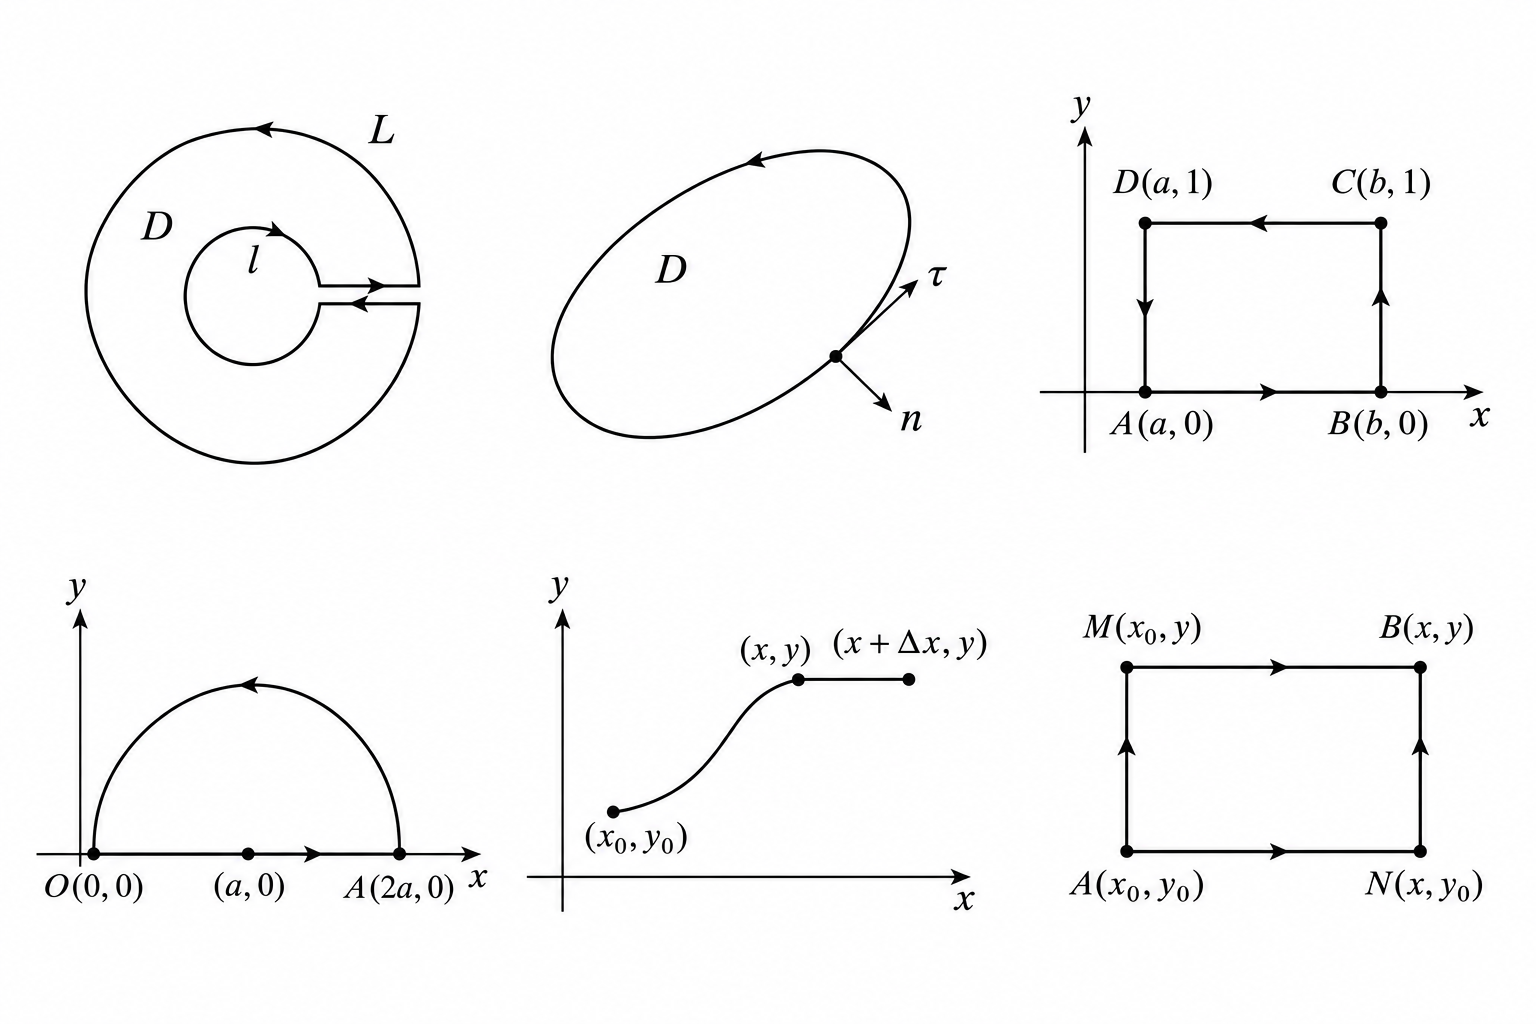
\includegraphics[width=0.2621\linewidth,viewport=77 551 429 917,clip]{figure/P2/green_diagrams_redrawn_hd.png}
\par}
\addvspace{3pt}
用连接内外边界的割线可把有洞区域切开。割线两岸的诱导方向相反，因此对应的曲线积分相互抵消；也可以先去掉宽度为 $\varepsilon$ 的窄条，再令 $\varepsilon\to0$。

\subsection*{Green 公式}
\begin{theorem}
设 $D$ 为平面有界单连通区域，边界 $\partial D$ 为分段光滑的简单闭曲线；$P,Q$ 在 $\overline D$ 的一个邻域内具有连续偏导数，则
\[
\oint_{\partial D}P\,\dd x+Q\,\dd y
=\displaystyle\iint_D\left(\frac{\partial Q}{\partial x}-\frac{\partial P}{\partial y}\right)\,\dd x\dd y,
\]
其中 $\partial D$ 取诱导定向，即逆时针方向。
\end{theorem}
\begin{proof}
先证明最简单的情形：$D$ 同时可表示为
\[
\begin{aligned}
D&=\{(x,y):a\le x\le b,\ y_1(x)\le y\le y_2(x)\}\\
&=\{(x,y):c\le y\le d,\ x_1(y)\le x\le x_2(y)\},
\end{aligned}
\]
其中边界函数分段光滑。由累次积分及 Newton--Leibniz 公式，
\begin{align*}
\displaystyle\iint_D Q_x\,\dd x\dd y
&=\int_c^d\dd y\int_{x_1(y)}^{x_2(y)}Q_x(x,y)\,\dd x\\
&=\int_c^d[Q(x_2(y),y)-Q(x_1(y),y)]\,\dd y.
\end{align*}
边界右侧由下向上，左侧由上向下，水平边上的 $\dd y=0$，所以
\[
\oint_{\partial D}Q\,\dd y
=\int_c^d Q(x_2(y),y)\,\dd y+\int_d^c Q(x_1(y),y)\,\dd y
=\displaystyle\iint_D Q_x\,\dd x\dd y.
\]
同样，
\[
\displaystyle\iint_D P_y\,\dd x\dd y
=\int_a^b[P(x,y_2(x))-P(x,y_1(x))]\,\dd x.
\]
边界下侧从左向右，上侧从右向左，竖直边上的 $\dd x=0$，因此
\[
\oint_{\partial D}P\,\dd x
=\int_a^bP(x,y_1(x))\,\dd x+\int_b^aP(x,y_2(x))\,\dd x
=-\displaystyle\iint_D P_y\,\dd x\dd y.
\]
相加即得所述公式。

若 $D$ 可有限分成上述类型的区域 $D_1,\ldots,D_N$，对每片分别使用公式并相加。每条内部公共边界恰出现两次且方向相反，故其积分抵消；余下的外边界恰为 $\partial D$。二重积分由区域可加性相加，得到 $D$ 上的公式。


% 按用户提供的局部引理、单位分解方法补全一般情形；展开坐标旋转和角点处理。
对一般分段光滑边界，下面用局部计算和单位分解补全证明。先说明所用概念。
\end{proof}


\begin{definition}
	设 $f$ 为开集 $U\subset\mathbb R^2$ 上的函数。称
	\[
	\operatorname{supp}f=\overline{\{p\in U:f(p)\ne0\}}^{\,U}
	\]
	为 $f$ 在 $U$ 中的支集，其中横线表示相对于 $U$ 的闭包。也就是说，支集由所有非零点及其在 $U$ 中的极限点组成；在支集之外，每一点都有一个邻域使 $f$ 恒为零。
	
	若 $\operatorname{supp}f$ 是包含于 $U$ 的紧集，则称 $f$ 在 $U$ 中具有紧支集。记 $K\Subset U$ 表示 $K$ 是包含于开集 $U$ 的紧集。此时 $K$ 与 $\mathbb R^2\setminus U$ 有正距离，因而紧支集函数在靠近 $U$ 外部的一带恒为零，可以在 $U$ 外延拓为零。
\end{definition}
\begin{lemma}[局部计算]
设 $V$ 是边界一点的局部邻域，在某个保持定向的正交坐标系中，$D\cap V$ 是一条 $C^1$ 图像曲线的一侧。若 $f\in C^1(V)$ 且 $\operatorname{supp}f\Subset V$，则将 $f$ 在 $V$ 外延拓为零后，有
\[
\oint_{\partial D} f\,\dd x
=-\displaystyle\iint_D f_y\,\dd x\dd y,
\qquad
\oint_{\partial D} f\,\dd y
=\displaystyle\iint_D f_x\,\dd x\dd y.
\]
若支集紧含于 $D$ 内，上述两式也成立，且等式两端均为零。
\end{lemma}
\begin{proof}
先设在原坐标中边界为 $y=\varphi(x)$，区域在其上方。因支集紧含于局部邻域，可以只在包含支集的有界矩形中积分，并在矩形外把函数记为零。于是
\begin{align*}
-\displaystyle\iint_D f_y\,\dd x\dd y
&=-\int\left[\int_{\varphi(x)}^{+\infty}f_y(x,y)\,\dd y\right]\,\dd x\\
&=\int f(x,\varphi(x))\,\dd x.
\end{align*}
这里无穷积分限只是简写，实际被积函数在有界范围外恒为零。区域在曲线上方时，正向边界从左向右，故右端就是 $\oint_{\partial D}f\,\dd x$。

为同时处理另一分量，令
\[
H(x)=\int_{\varphi(x)}^{+\infty} f(x,y)\,\dd y.
\]
由变限积分求导公式，
\[
H'(x)=\int_{\varphi(x)}^{+\infty}f_x(x,y)\,\dd y
-f(x,\varphi(x))\varphi'(x).
\]
$H$ 在一个有界区间外为零，所以 $\int H'(x)\,\dd x=0$，从而
\[
\displaystyle\iint_D f_x\,\dd x\dd y
=\int f(x,\varphi(x))\varphi'(x)\,\dd x
=\oint_{\partial D}f\,\dd y.
\]
若区域在曲线下方，则对 $y$ 的积分从 $-\infty$ 到 $\varphi(x)$，正向边界也改为从右向左。两处符号相应改变，所得两式不变。

现在说明旋转坐标的情形。上面两式对任意紧支集向量场 $\boldsymbol A=(A_1,A_2)$ 相加，等价于局部的通量等式
\[
\oint_{\partial D}\boldsymbol A\cdot\boldsymbol n\,\dd s
=\displaystyle\iint_D(\partial_xA_1+\partial_yA_2)\,\dd x\dd y.
\]
作保持定向的正交变换 $p=R\widetilde p+b$，令 $\widetilde{\boldsymbol A}(\widetilde p)=R^{\mathsf T}\boldsymbol A(R\widetilde p+b)$。正交变换保持长度、面积和内积，单位外法向量按同一矩阵变换，且由链式法则
\[
D\widetilde{\boldsymbol A}=R^{\mathsf T}(D\boldsymbol A)R,
\quad
\partial_{\widetilde x}\widetilde A_1+\partial_{\widetilde y}\widetilde A_2
=\partial_xA_1+\partial_yA_2.
\]
其中 $D\boldsymbol A$ 是向量场的导数矩阵，后一等式可由 $RR^{\mathsf T}=I$ 直接展开得到。因此通量等式不因旋转改变。分别取 $\boldsymbol A=(0,-f)$ 和 $(f,0)$，再用 $\boldsymbol n\,\dd s=(\dd y,-\dd x)$，就得到原坐标中的两条结论。

若支集紧含于 $D$，边界积分为零；在包含支集的矩形中先对相应变量积分，利用矩形边上 $f=0$，两个偏导数的面积积分也均为零。
\end{proof}

\begin{definition}
设紧集 $K$ 被有限个开集 $V_1,\ldots,V_N$ 覆盖。若光滑非负函数 $\rho_1,\ldots,\rho_N$ 在 $K$ 的某个邻域内满足
\[
\sum_{i=1}^N\rho_i=1,\qquad \operatorname{supp}\rho_i\Subset V_i,
\]
则称这些函数构成从属于该覆盖的光滑单位分解。它把一个函数分成各自只在一个局部邻域内起作用的有限个函数。
\end{definition}
这样的单位分解可以构造如下。对每个 $p\in K$ 取小球，使其二倍球的闭包仍在某个 $V_i$ 中；由紧性选出有限个小球覆盖 $K$。在每个二倍球中取光滑非负函数 $\eta_j$，使它在对应小球上严格为正，在二倍球外为零。例如，平移缩放后可用
\[
\eta(p)=
\begin{cases}
\exp\bigl(-1/(1-|p|^2)\bigr),&|p|<1,\\
0,&|p|\ge1.
\end{cases}
\]
令 $h=\sum_j\eta_j$，则 $h>0$ 于 $K$ 的一个邻域。再取光滑函数 $\chi$，使它在 $K$ 附近等于 $1$，且支集紧含于 $\{h>0\}$：可取充分小的 $c>0$ 使 $h>2c$ 于 $K$，再令 $\chi=\psi(h)$，其中光滑函数 $\psi$ 在 $[0,c]$ 为零，在 $[2c,+\infty)$ 为 $1$。于是 $\chi\eta_j/h$ 在 $h>0$ 处定义、其余处置零，便得到所需函数；把属于同一 $V_i$ 的项相加即得 $\rho_i$。

\begin{proof}[Green 公式一般情形的证明]
先设 $P,Q$ 在所有角点附近为零。它们的支集与 $\overline D$ 的交集是紧集，且避开有限个角点。在光滑边界点处，由正则性及隐函数定理，可以选取保持定向的正交坐标，使边界局部成为 $C^1$ 图像。用这些边界邻域和完全位于 $D$ 内的邻域覆盖该紧集，取有限子覆盖及相应单位分解。

令 $P_i=\rho_iP$、$Q_i=\rho_iQ$，则在 $\overline D$ 上有
\[
P=\sum_iP_i,\qquad Q=\sum_iQ_i,
\qquad P_y=\sum_i(P_i)_y,\qquad Q_x=\sum_i(Q_i)_x.
\]
对每一项用局部引理；支集在内部的项两端均为零。逐项相加，得到
\begin{align*}
\oint_{\partial D}P\,\dd x+Q\,\dd y
&=\sum_i\oint_{\partial D}(P_i\,\dd x+Q_i\,\dd y)\\
&=\sum_i\displaystyle\iint_D[(Q_i)_x-(P_i)_y]\,\dd x\dd y\\
&=\displaystyle\iint_D(Q_x-P_y)\,\dd x\dd y.
\end{align*}

最后去掉在角点附近为零的限制。记角点为 $c_1,\ldots,c_m$。取光滑截断函数 $\theta_\varepsilon$，使它在每个 $B(c_j,\varepsilon)$ 内为零，在所有 $B(c_j,2\varepsilon)$ 外为 $1$，且
\[
0\le\theta_\varepsilon\le1,\qquad
|\nabla\theta_\varepsilon|\le C/\varepsilon.
\]
这里 $B(c,r)$ 为以 $c$ 为中心、半径为 $r$ 的开圆盘，$\nabla\theta=(\theta_x,\theta_y)$。可将固定光滑径向截断函数缩放后取有限个因子的乘积得到上述函数。

对 $P_\varepsilon=\theta_\varepsilon P$、$Q_\varepsilon=\theta_\varepsilon Q$ 使用已经证明的公式。它们与原函数的差只出现在角点的 $2\varepsilon$ 邻域内。这些邻域的总面积为 $O(\varepsilon^2)$；正则 $C^1$ 边界弧在其中的总长度为 $O(\varepsilon)$，因为弧在角点每一侧均可表示为导数有界的局部图像。$P,Q$ 及其一阶偏导数在 $\overline D$ 附近有界，所以边界积分之差为 $O(\varepsilon)$。

另一方面，
\[
(Q_\varepsilon)_x-(P_\varepsilon)_y
=\theta_\varepsilon(Q_x-P_y)
+(\theta_\varepsilon)_xQ-(\theta_\varepsilon)_yP.
\]
第一项与 $Q_x-P_y$ 的面积积分之差为 $O(\varepsilon^2)$；后两项的积分绝对值不超过常数乘以 $\varepsilon^{-1}\varepsilon^2$，因而为 $O(\varepsilon)$。令 $\varepsilon\to0$，就得到原来的 $P,Q$ 所满足的 Green 公式。一般分段光滑边界的证明完成。
\end{proof}

Green 公式也适用于边界由有限条互不相交的分段光滑 Jordan 曲线组成的有洞区域。以一个洞为例，外边界记为 $L$，内边界记为 $l$，取割线 $MN$ 后，割线两岸的积分抵消，故
\[
\begin{aligned}
\displaystyle\iint_D(Q_x-P_y)\,\dd x\dd y
&=\left(\int_L+\int_{MN}+\int_l+\int_{NM}\right)(P\,\dd x+Q\,\dd y)\\
&=\left(\int_L+\int_l\right)(P\,\dd x+Q\,\dd y)
=\oint_{\partial D}P\,\dd x+Q\,\dd y.
\end{aligned}
\]
这里 $L$ 逆时针、$l$ 顺时针，与区域的诱导定向一致。

\subsection*{Green 公式的几种应用}
\begin{enumerate}
\item 记正向边界的单位切向量为 $\boldsymbol\tau$，单位外法向量为 $\boldsymbol n$。若 $\boldsymbol\tau=(\tau_x,\tau_y)$，则 $\boldsymbol n=(\tau_y,-\tau_x)$，故
\[
\cos(\vect n,y)=-\cos(\vect \tau,x),\qquad \cos(\vect n,x)=\sin(\vect \tau,x),
\]
其中后一式把切向角理解为有向角。令 $P=-G,Q=F$，得到
\begin{align*}
\displaystyle\iint_D(F_x+G_y)\,\dd x\dd y
&=\oint_{\partial D}F\,\dd y-G\,\dd x\\
&=\oint_{\partial D}[F\cos(\vect n,x)+G\cos(\vect n,y)]\,\dd s.
\end{align*}
\par\addvspace{3pt}
{\centering
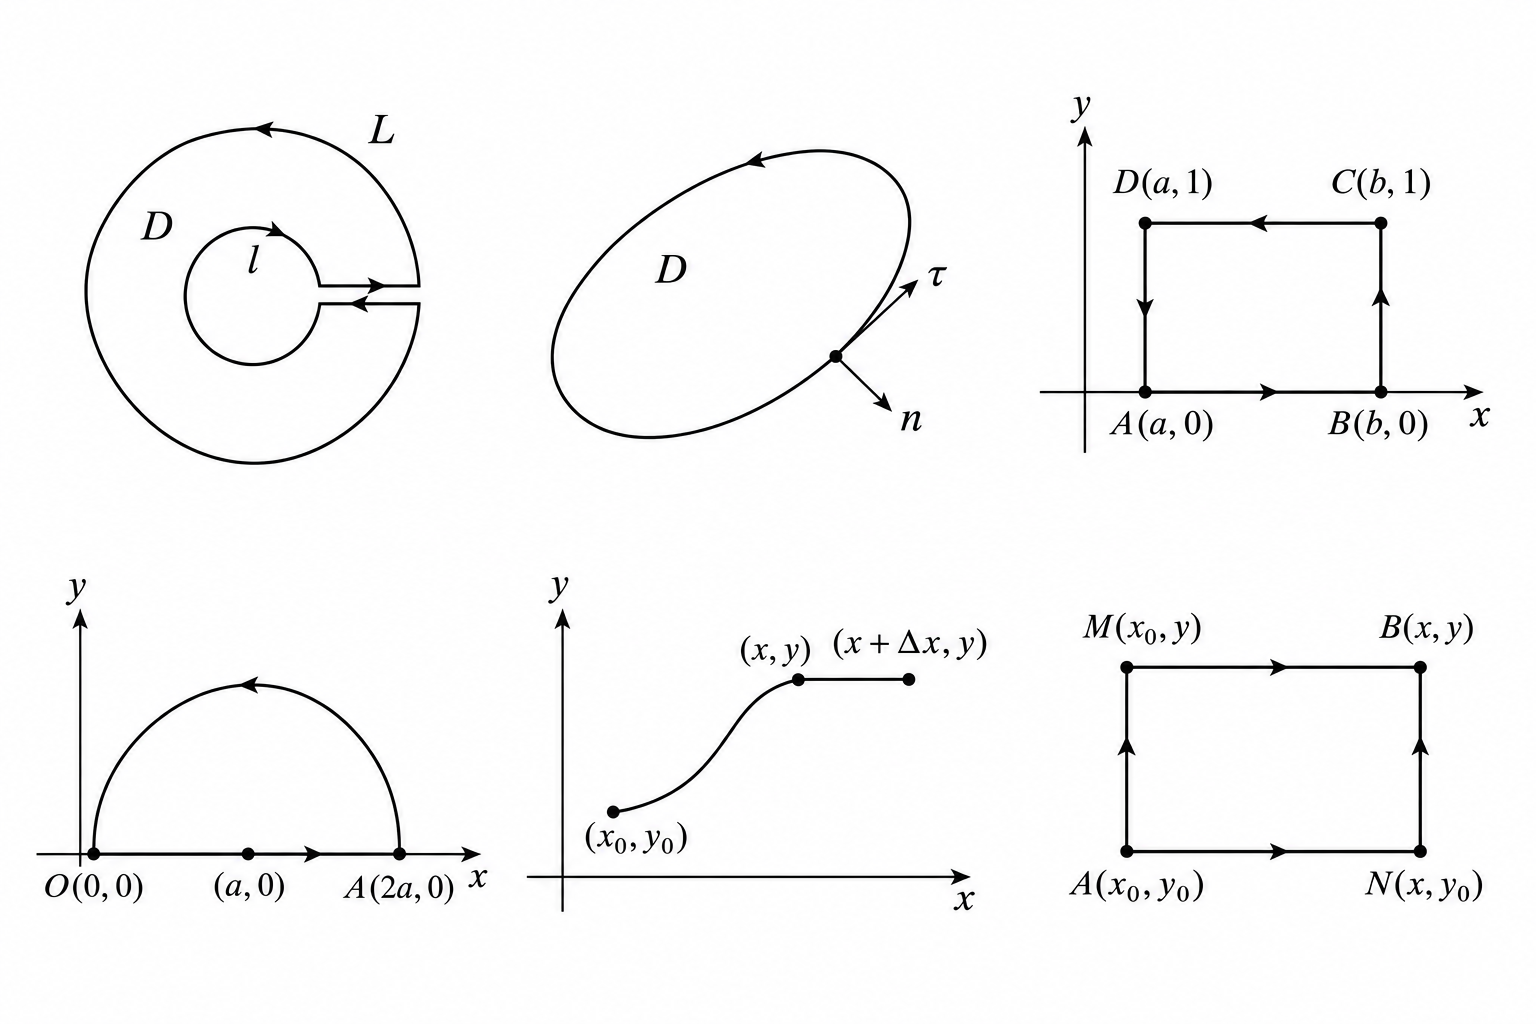
\includegraphics[width=0.2884\linewidth,viewport=543 577 955 883,clip]{figure/P2/green_diagrams_redrawn_hd.png}
\par}
\addvspace{3pt}
\item Green 公式推广了 Newton--Leibniz 公式。设 $f\in C^1([a,b])$，在 $D=[a,b]\times[0,1]$ 上取 $P=0,Q=f(x)$，则
\[
\displaystyle\iint_Df'(x)\,\dd x\dd y=\oint_{\partial D}f(x)\,\dd y.
\]
\par\addvspace{3pt}
{\centering
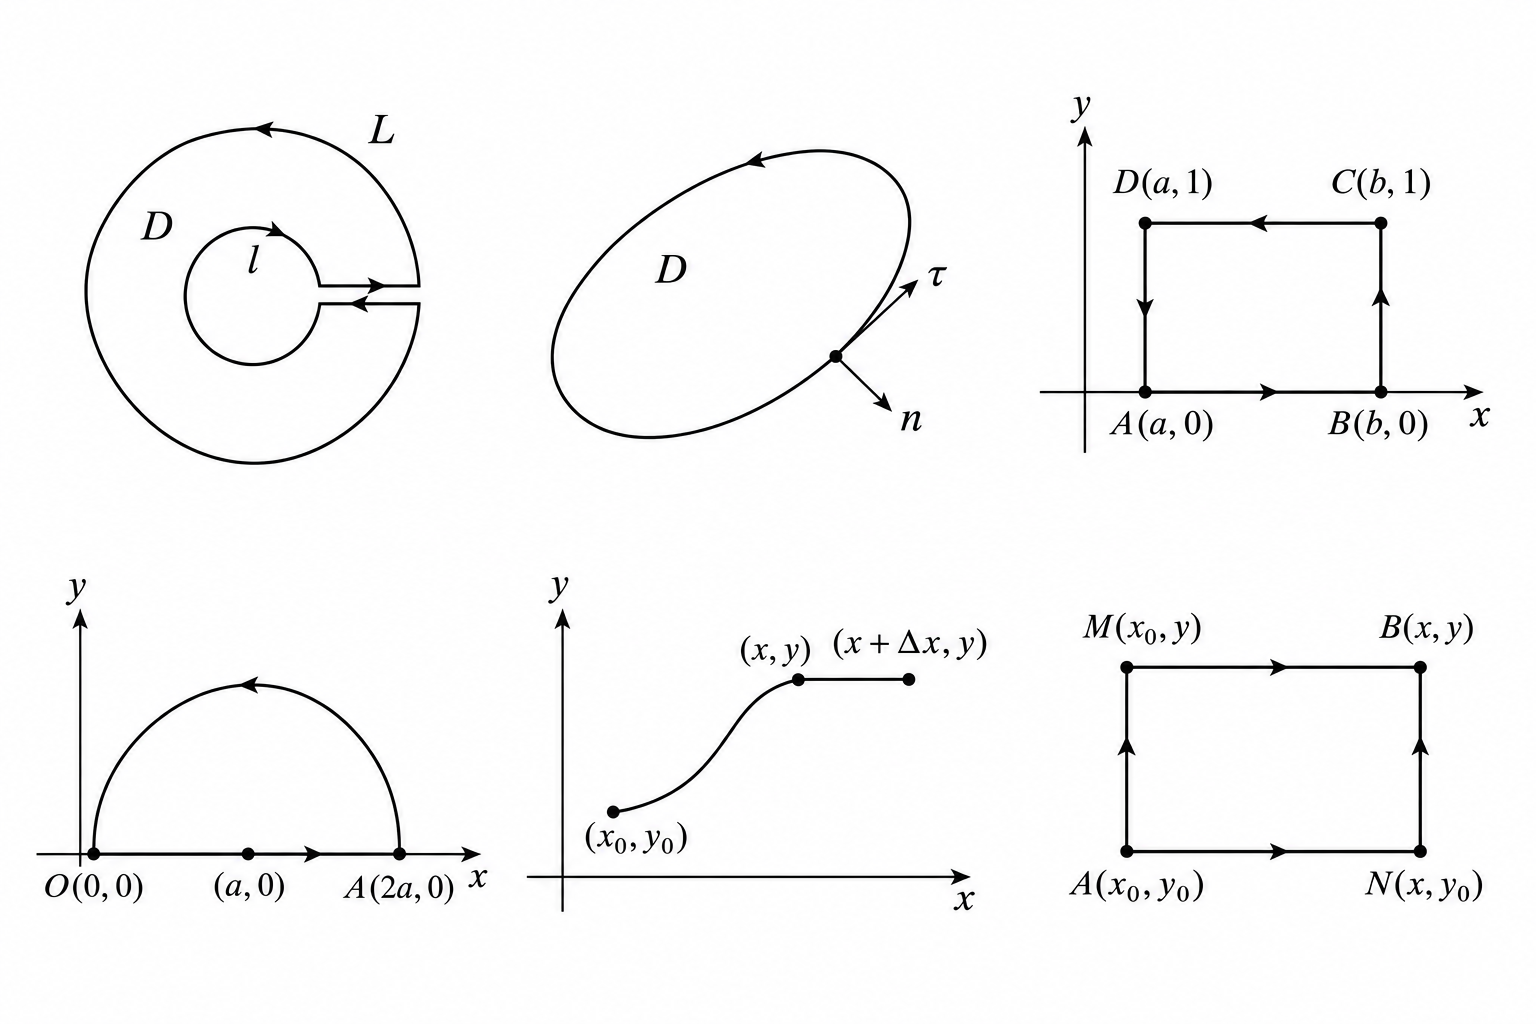
\includegraphics[width=0.45\linewidth,viewport=1032 563 1498 935,clip]{figure/P2/green_diagrams_redrawn_hd.png}
\par}
\addvspace{3pt}
左端等于 $\displaystyle\int_a^bf'(x)\,\dd x$。右端的两条水平边贡献为零，右侧竖边向上，左侧竖边向下，因而
\[
\oint_{\partial D}f(x)\,\dd y=\int_0^1 f(b)\,\dd y+\int_1^0 f(a)\,\dd y=f(b)-f(a).
\]
于是 $\displaystyle\int_a^bf'(x)\,\dd x=f(b)-f(a)$。
\item 若 $D$ 的边界为分段光滑简单闭曲线，面积为 $S$，则
\[
S=\displaystyle\iint_D1\,\dd x\dd y
=\oint_{\partial D}x\,\dd y
=-\oint_{\partial D}y\,\dd x
=\frac12\oint_{\partial D}(x\,\dd y-y\,\dd x).
\]
\end{enumerate}
% 原文面积公式的证明留给读者。
\begin{proof}
在 Green 公式中依次取 $(P,Q)=(0,x)$、$(-y,0)$ 和 $(-y/2,x/2)$，三次均有 $Q_x-P_y=1$，故分别得到三条边界积分公式。
\end{proof}

\begin{example}
计算
\[
I=\int_L(e^x\sin y-my)\,\dd x+(e^x\cos y-m)\,\dd y,
\]
其中 $L$ 为圆 $(x-a)^2+y^2=a^2$（$a>0$）的上半圆周，方向从 $A(2a,0)$ 到 $O(0,0)$。
\end{example}
\begin{solution}
$L$ 不是闭曲线，补入从 $O$ 到 $A$ 的直线段 $\overrightarrow{OA}$，得到上半圆域 $D$ 的正向边界。
\par\addvspace{3pt}
{\centering
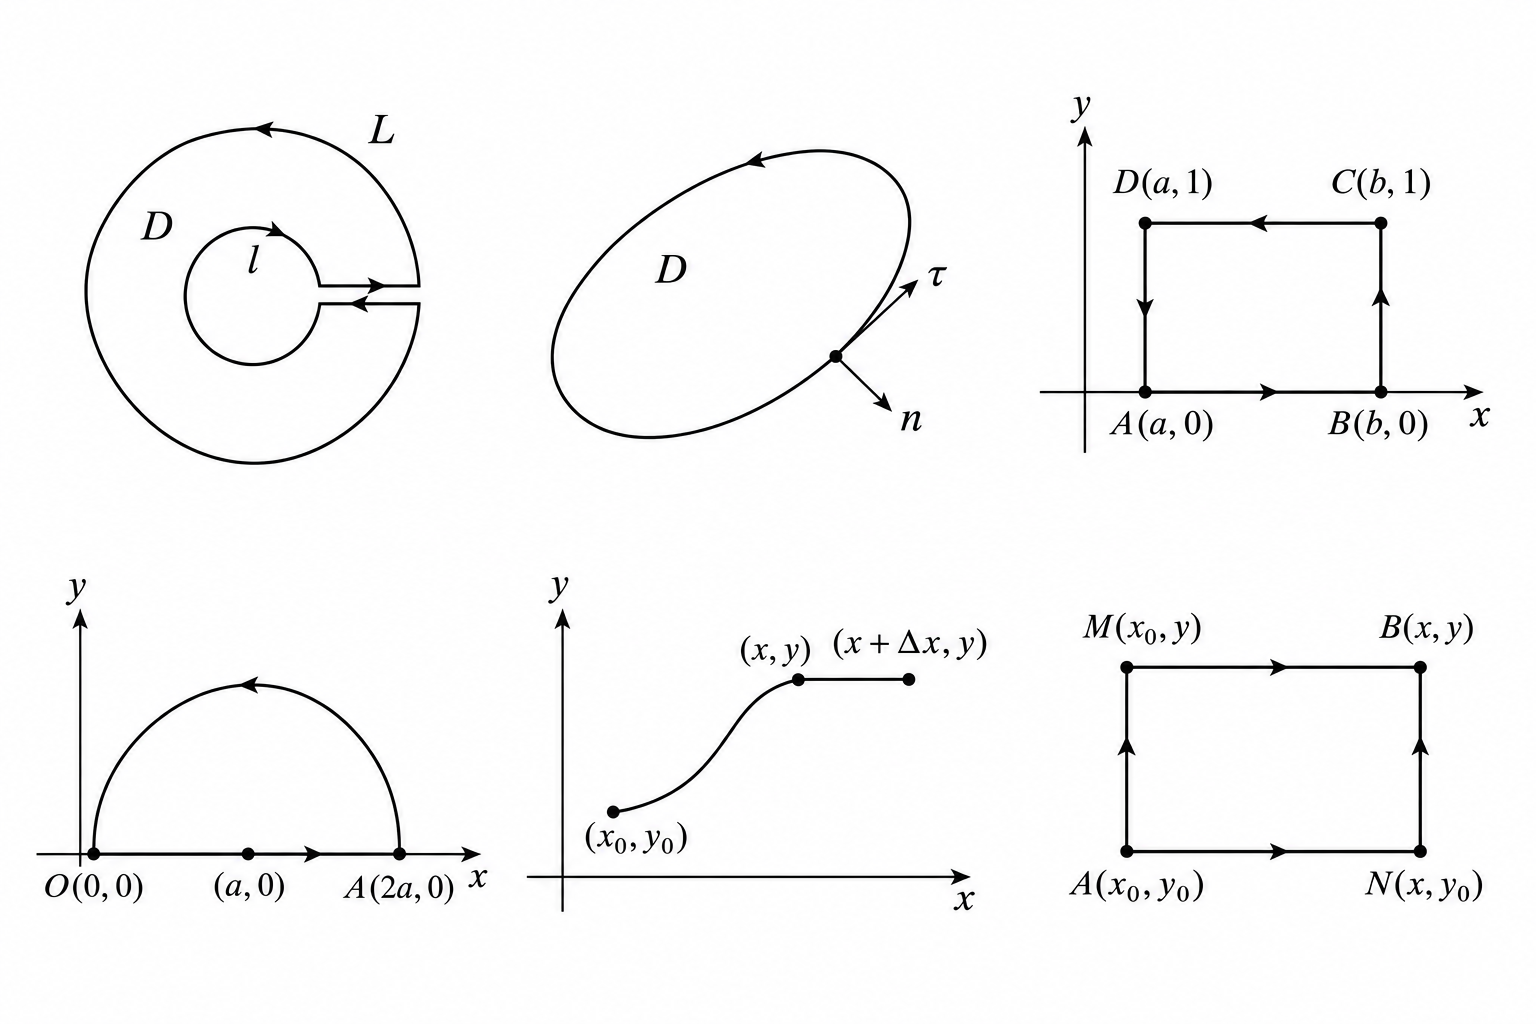
\includegraphics[width=0.5126\linewidth,viewport=29 112 495 453,clip]{figure/P2/green_diagrams_redrawn_hd.png}
\par}
\addvspace{3pt}
取 $P=e^x\sin y-my$、$Q=e^x\cos y-m$，则
\[
P_y=e^x\cos y-m,\qquad Q_x=e^x\cos y.
\]
由 Green 公式，
\[
I+\int_{\overrightarrow{OA}}P\,\dd x+Q\,\dd y
=m\displaystyle\iint_D1\,\dd x\dd y=\frac{m\pi a^2}{2}.
\]
沿 $\overrightarrow{OA}$，$y=0$、$\dd y=0$、$P(x,0)=0$，故补线积分为零。因此
\[
I=\frac{m\pi a^2}{2}.
\]
\end{solution}

\subsection*{曲线积分与路径无关}
\begin{definition}
设 $D$ 为平面区域，$P,Q$ 在 $D$ 上连续。若对任意 $A,B\in D$，曲线积分 $\int_LP\,\dd x+Q\,\dd y$ 只与端点 $A,B$ 有关，与 $D$ 内连接它们的分段光滑路径 $L$ 无关，则称该曲线积分与路径无关；否则称为与路径有关。
\end{definition}
\begin{theorem}[Green 定理]
(Green 定理)设 $D$ 为平面单连通区域，$P,Q\in C^1(D)$。以下四个命题等价：
\begin{enumerate}
\item 对 $D$ 内任意分段光滑闭曲线 $L$，有 $\displaystyle\oint_LP\,\dd x+Q\,\dd y=0$；
\item 曲线积分 $\displaystyle\int_LP\,\dd x+Q\,\dd y$ 与路径无关；
\item 存在 $D$ 上的可微函数 $U$，使 $\dd U=P\,\dd x+Q\,\dd y$；
\item 在 $D$ 内 $P_y=Q_x$。
\end{enumerate}
其中第三条称 $P\,\dd x+Q\,\dd y$ 为 $U$ 的全微分，并称 $U$ 为该 $1$-形式的原函数。
\end{theorem}
\begin{proof}
\begin{enumerate}
\item[$(1)\Rightarrow(2)$] 取任意从 $A$ 到 $B$ 的两条路径 $L_1,L_2$，闭曲线 $C=L_1+(-L_2)$ 满足
\[
0=\oint_C P\,\dd x+Q\,\dd y
=\int_{L_1}P\,\dd x+Q\,\dd y-\int_{L_2}P\,\dd x+Q\,\dd y.
\]
故两条路径的积分相等。
\item[$(2)\Rightarrow(3)$] 固定 $(x_0,y_0)\in D$，定义
\[
U(x,y)=\int_{(x_0,y_0)}^{(x,y)}P\,\dd x+Q\,\dd y.
\]
区域内两点可用分段光滑路径连接，路径无关性保证定义唯一。由于 $D$ 开，在 $(x,y)$ 附近的一小段水平线仍位于 $D$ 内，于是
\[
\frac{U(x+\Delta x,y)-U(x,y)}{\Delta x}
=\frac1{\Delta x}\int_x^{x+\Delta x}P(t,y)\,\dd t\longrightarrow P(x,y).
\]
\par\addvspace{3pt}
{\centering
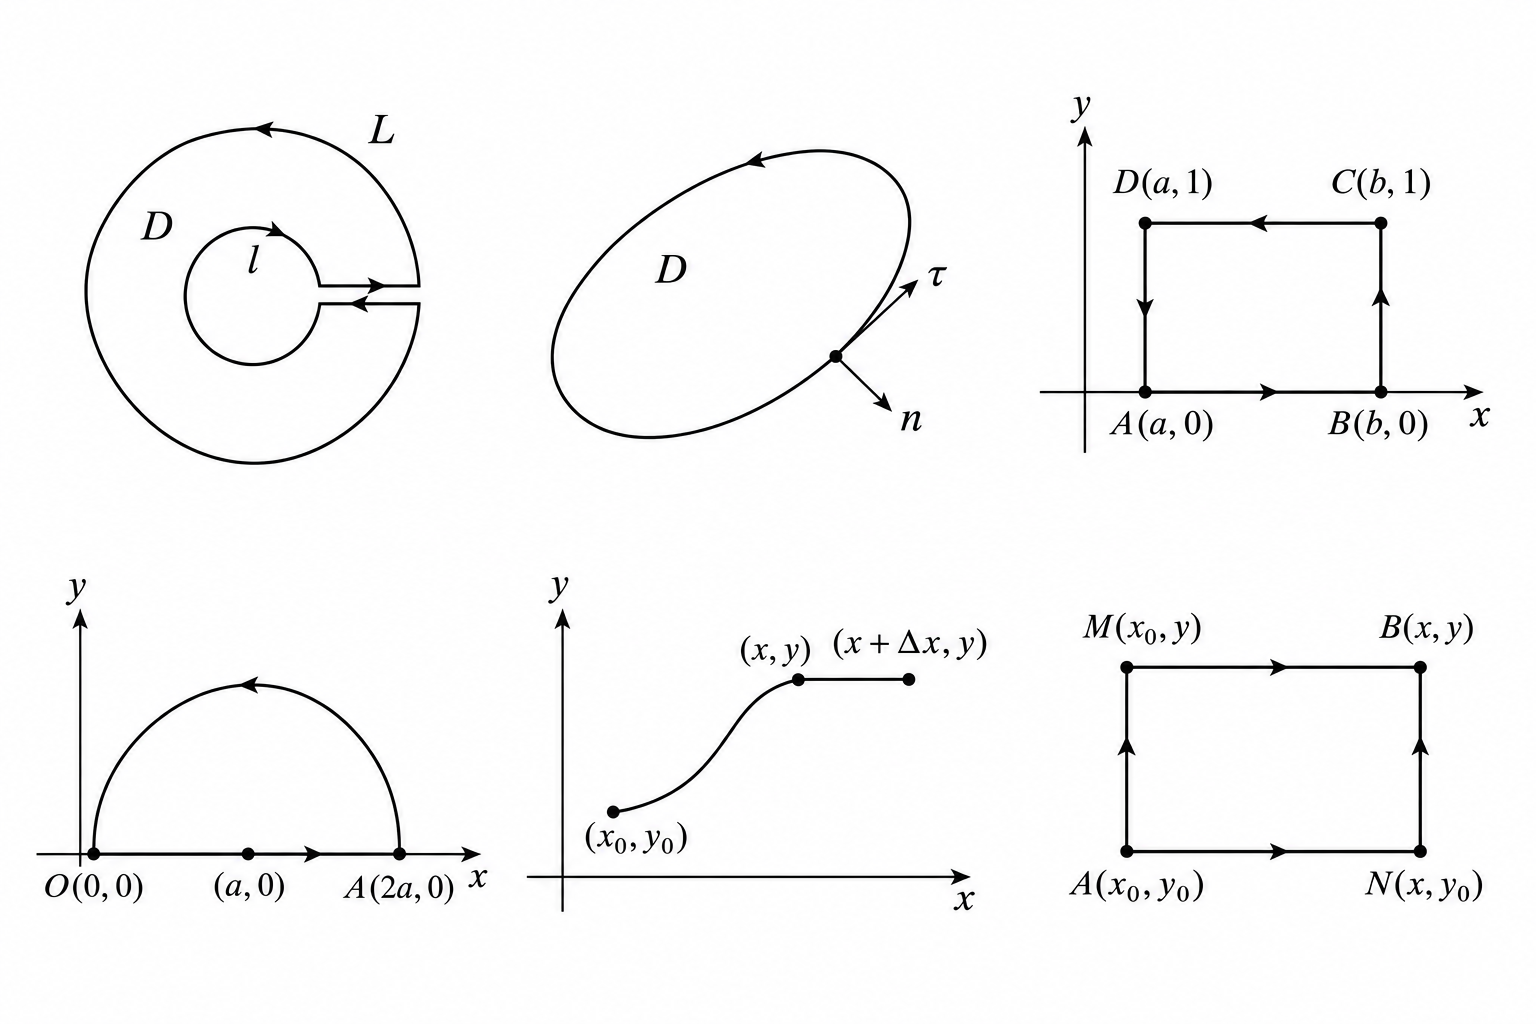
\includegraphics[width=0.45\linewidth,viewport=519 104 994 455,clip]{figure/P2/green_diagrams_redrawn_hd.png}
\par}
\addvspace{3pt}
沿竖直短线段同理得 $U_y=Q$。因 $P,Q$ 连续，$U$ 可微，且 $\dd U=P\,\dd x+Q\,\dd y$。
\item[$(3)\Rightarrow(4)$] 由 $U_x=P,U_y=Q$ 及 $P,Q\in C^1(D)$，可知 $U\in C^2(D)$。混合偏导数相等，故
\[
P_y=U_{xy}=U_{yx}=Q_x.
\]
\item[$(4)\Rightarrow(1)$] 先设 $L$ 为简单闭曲线。单连通性保证其围成的内部 $\widetilde D$ 仍在 $D$ 中，由 Green 公式，
\[
\oint_LP\,\dd x+Q\,\dd y
=\pm\displaystyle\iint_{\widetilde D}(Q_x-P_y)\,\dd x\dd y=0.
\]
% 以下补足原图从简单闭曲线到一般闭路径的适用范围。
若 $L$ 是一般分段光滑闭路径，先对有限自交的闭折线按交点分解成有限条简单闭折线；每条积分均为零，相加仍为零。再在 $D$ 内用闭折线逼近 $L$：在每段 $C^1$ 参数区间上取足够细的划分并连接相邻点。由于路径像为 $D$ 内的紧集，细划分的弦段仍在 $D$ 内；由参数导数的一致连续性，折线的分段导数在各光滑段上一致逼近原导数，位置也一致逼近原路径。因此 $P,Q$ 的连续性保证折线积分趋于 $L$ 上的积分。若折线有退化重合边，可作任意小顶点扰动使交点有限，积分随扰动连续变化，结论仍成立。故一般闭路径的积分也为零。
\end{enumerate}
\end{proof}

\begin{theorem}
设 $D$ 为平面单连通区域，$P,Q$ 在 $D$ 上连续。曲线积分与路径无关的充分必要条件是 $P\,\dd x+Q\,\dd y$ 在 $D$ 上存在原函数 $U$。此时对于任意从 $A(x_A,y_A)$ 到 $B(x_B,y_B)$ 的分段光滑路径，有
\[
\int_A^B P\,\dd x+Q\,\dd y=U(x_B,y_B)-U(x_A,y_A).
\]
\end{theorem}
\begin{proof}
若积分与路径无关，按前一定理的构造定义 $U$；该构造只需 $P,Q$ 连续，就有 $U_x=P,U_y=Q$。取一条从基点到 $A$ 的路径 $l$，再接上从 $A$ 到 $B$ 的路径 $L$，则
\[
U(A)=\int_lP\,\dd x+Q\,\dd y,\qquad
U(B)=\int_{l+L}P\,\dd x+Q\,\dd y.
\]
相减即得积分等于 $U(B)-U(A)$。

反之，若存在原函数 $U$，沿光滑路径 $L:(x(t),y(t))$，$a\le t\le b$，由链式法则，
\begin{align*}
\int_LP\,\dd x+Q\,\dd y
&=\int_a^b[P(x(t),y(t))x'(t)+Q(x(t),y(t))y'(t)]\,\dd t\\
&=\int_a^b\frac{\dd}{\dd t}U(x(t),y(t))\,\dd t
=U(B)-U(A).
\end{align*}
分段光滑路径逐段使用此式，中间端点值抵消，结论相同。因此积分与路径无关。
\end{proof}

求原函数常用两条折线路径。固定基点 $A=(x_0,y_0)$，令 $B=(x,y)$，$N=(x,y_0)$、$M=(x_0,y)$。
\par\addvspace{3pt}
{\centering
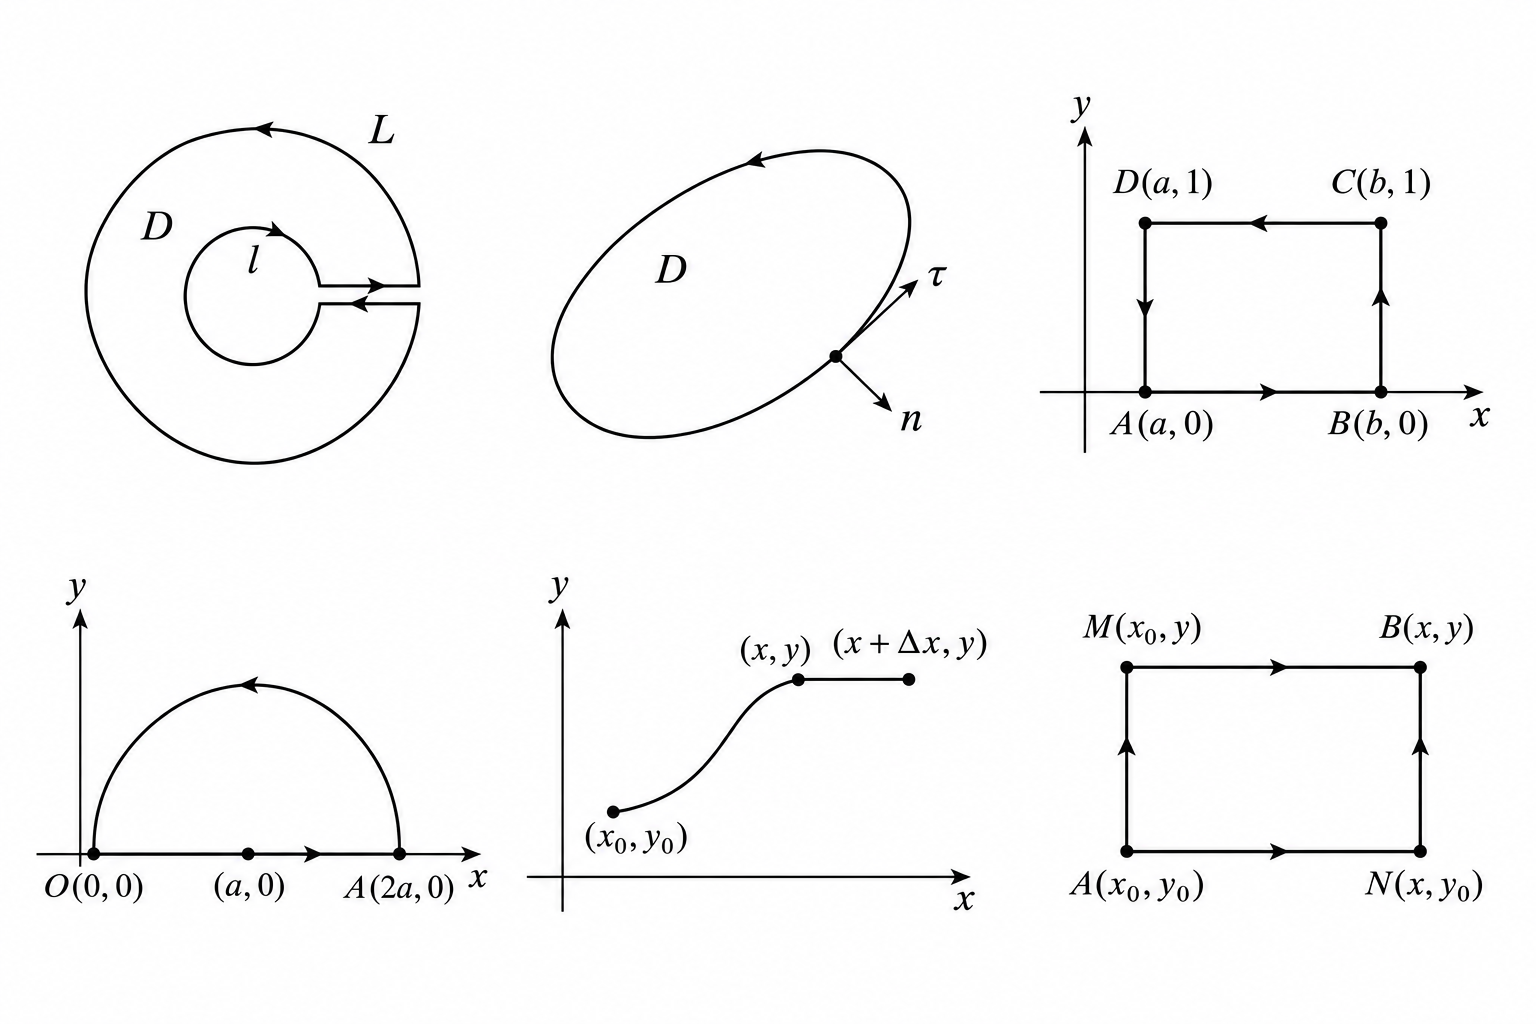
\includegraphics[width=0.4\linewidth,viewport=1062 114 1490 419,clip]{figure/P2/green_diagrams_redrawn_hd.png}
\par}
\addvspace{3pt}
当所用折线全部位于 $D$ 内时，沿 $ANB$ 积分得到
\[
U(x,y)=\int_{x_0}^x P(t,y_0)\,\dd t+\int_{y_0}^y Q(x,s)\,\dd s+c.
\]
沿 $AMB$ 则得到
\[
U(x,y)=\int_{y_0}^y Q(x_0,s)\,\dd s+\int_{x_0}^x P(t,y_0)\,\dd t+c,
\qquad c=U(x_0,y_0).
\]
%

% 第4节：微分形式的外微分
% !TEX root = ../../../../main.tex
% 第二部分第四章第四节：微分形式的外微分
\section{微分形式的外微分}

\subsection*{外微分}
设 $U\subset\mathbb R^n$ 为区域，$f$ 为 $U$ 上具有连续偏导数的函数，则其全微分为
\[
\dd f=\sum_{i=1}^n\frac{\partial f}{\partial x_i}\,\dd x_i.
\]
这可以理解为对一个 $0$-形式进行微分，得到一个 $1$-形式。

\begin{definition}
设 $\omega$ 为 $U$ 上的 $k$-形式，标准形式为
\[
\omega=\sum_{1\le i_1<\cdots<i_k\le n}
 g_{i_1\cdots i_k}(x)\,\dd x_{i_1}\wedge\cdots\wedge\dd x_{i_k},
\]
且各系数函数具有连续偏导数。定义 $\omega$ 的\textbf{外微分}为
\begin{align*}
\dd\omega
&=\sum_{1\le i_1<\cdots<i_k\le n}
 (\dd g_{i_1\cdots i_k})\wedge\dd x_{i_1}\wedge\cdots\wedge\dd x_{i_k}\\
&=\sum_{1\le i_1<\cdots<i_k\le n}\sum_{j=1}^n
 \frac{\partial g_{i_1\cdots i_k}}{\partial x_j}\,
 \dd x_j\wedge\dd x_{i_1}\wedge\cdots\wedge\dd x_{i_k}.
\end{align*}
它是一个 $(k+1)$-形式。对 $0$-形式，外微分就是函数的全微分；当 $k=n$ 时，每项都有重复的微分符号，因而 $\dd\omega=0$。

对不同次数的形式之和 $\omega=\omega_0+\cdots+\omega_n$，其中 $\omega_i$ 为 $i$-形式，定义
\[
\dd\omega=\dd\omega_0+\cdots+\dd\omega_n.
\]
\end{definition}
% 外微分降低系数的可微阶数，不能无条件把 C^1 系数空间映入自身。
外微分的系数是原系数的一阶偏导数，因此原系数为 $C^1$ 时，所得系数一般仅连续。以下涉及一次外微分时假设系数为 $C^1$；涉及连续两次外微分时假设系数为 $C^2$，从而两次运算都有意义。

\begin{proposition}
外微分关于实常数是线性的：若 $a,b\in\mathbb R$，则
\[
\dd(a\omega+b\eta)=a\,\dd\omega+b\,\dd\eta.
\]
而且对任意常系数基形式，有
\[
\dd(\dd x_{i_1}\wedge\cdots\wedge\dd x_{i_k})=0.
\]
\end{proposition}
\begin{proof}
将 $a\omega+b\eta$ 按同一组基展开，其系数是一一对应的系数函数的线性组合。由函数微分的线性性，逐项微分即得第一个等式。

基形式的系数为常数 $1$，由定义，
\[
\dd(\dd x_{i_1}\wedge\cdots\wedge\dd x_{i_k})
=(\dd1)\wedge\dd x_{i_1}\wedge\cdots\wedge\dd x_{i_k}=0.
\]
\end{proof}

\begin{example}
设 $\omega=P(x,y)\,\dd x+Q(x,y)\,\dd y$ 为平面上的 $1$-形式，则
\begin{align*}
\dd\omega
&=(\dd P)\wedge\dd x+(\dd Q)\wedge\dd y\\
&=(P_x\,\dd x+P_y\,\dd y)\wedge\dd x
 +(Q_x\,\dd x+Q_y\,\dd y)\wedge\dd y\\
&=P_y\,\dd y\wedge\dd x+Q_x\,\dd x\wedge\dd y\\
&=(Q_x-P_y)\,\dd x\wedge\dd y.
\end{align*}
\end{example}

\begin{example}
设 $\omega=P(x,y,z)\,\dd x+Q(x,y,z)\,\dd y+R(x,y,z)\,\dd z$ 为空间中的 $1$-形式，则
\begin{align*}
\dd\omega
&=(\dd P)\wedge\dd x+(\dd Q)\wedge\dd y+(\dd R)\wedge\dd z\\
&=(P_x\,\dd x+P_y\,\dd y+P_z\,\dd z)\wedge\dd x\\
&\quad+(Q_x\,\dd x+Q_y\,\dd y+Q_z\,\dd z)\wedge\dd y\\
&\quad+(R_x\,\dd x+R_y\,\dd y+R_z\,\dd z)\wedge\dd z\\
&=(R_y-Q_z)\,\dd y\wedge\dd z
 +(P_z-R_x)\,\dd z\wedge\dd x\\
&\quad+(Q_x-P_y)\,\dd x\wedge\dd y.
\end{align*}
\end{example}

\begin{example}
设
\[
\omega=P(x,y,z)\,\dd y\wedge\dd z
+Q(x,y,z)\,\dd z\wedge\dd x
+R(x,y,z)\,\dd x\wedge\dd y
\]
为空间中的 $2$-形式，则
\begin{align*}
\dd\omega
&=(\dd P)\wedge\dd y\wedge\dd z
 +(\dd Q)\wedge\dd z\wedge\dd x
 +(\dd R)\wedge\dd x\wedge\dd y\\
&=P_x\,\dd x\wedge\dd y\wedge\dd z
 +Q_y\,\dd y\wedge\dd z\wedge\dd x
 +R_z\,\dd z\wedge\dd x\wedge\dd y\\
&=(P_x+Q_y+R_z)\,\dd x\wedge\dd y\wedge\dd z.
\end{align*}
这里每个含有重复微分符号的项均为零；将后两项的符号次序改为 $\dd x\wedge\dd y\wedge\dd z$，各需交换两次，所以符号均为正。
\end{example}

\begin{proposition}
若 $\omega$ 为 $k$-形式，$\eta$ 为 $l$-形式，且系数具有连续偏导数，则
\[
\dd(\omega\wedge\eta)
=\dd\omega\wedge\eta+(-1)^k\omega\wedge\dd\eta.
\]
\end{proposition}
\begin{proof}
由外微分的线性性和外积的双线性性，只需证明
\[
\omega=a(x)\,\dd x_I,\qquad \eta=b(x)\,\dd x_J,
\]
其中 $\dd x_I=\dd x_{i_1}\wedge\cdots\wedge\dd x_{i_k}$，$\dd x_J=\dd x_{j_1}\wedge\cdots\wedge\dd x_{j_l}$ 的情形。

由函数微分的乘积法则，
\begin{align*}
\dd(\omega\wedge\eta)
&=\dd(ab)\wedge\dd x_I\wedge\dd x_J\\
&=b\,\dd a\wedge\dd x_I\wedge\dd x_J
 +a\,\dd b\wedge\dd x_I\wedge\dd x_J.
\end{align*}
第一项为 $\dd\omega\wedge\eta$。第二项中，将 $1$-形式 $\dd b$ 移到 $k$ 个微分符号之后，需要交换 $k$ 次，故
\[
a\,\dd b\wedge\dd x_I\wedge\dd x_J
=(-1)^ka\,\dd x_I\wedge\dd b\wedge\dd x_J
=(-1)^k\omega\wedge\dd\eta.
\]
两项相加即得结论。若两组指标有重复，相关外积为零，上述等式仍成立。
\end{proof}

\begin{proposition}
若微分形式 $\omega$ 的各系数函数具有二阶连续偏导数，记 $\dd^2\omega=\dd(\dd\omega)$，则
\[
\dd^2\omega=0.
\]
\end{proposition}
\begin{proof}
先对 $C^2$ 函数 $a$ 计算：
\[
\dd^2a=\sum_{i=1}^n\sum_{j=1}^n
 \frac{\partial^2a}{\partial x_j\partial x_i}\,\dd x_j\wedge\dd x_i.
\]
当 $i=j$ 时，$\dd x_i\wedge\dd x_i=0$。当 $i\ne j$ 时，把 $(i,j)$ 和 $(j,i)$ 对应的两项合并，混合偏导数相等而外积符号相反，所以它们的和为零。因此 $\dd^2a=0$。

对一般形式，由线性性只需考虑 $\omega=a\,\dd x_I$。由外微分定义，$\dd\omega=\dd a\wedge\dd x_I$；再用乘积公式以及 $\dd(\dd x_I)=0$，得到
\begin{align*}
\dd^2\omega
&=\dd(\dd a\wedge\dd x_I)\\
&=\dd^2a\wedge\dd x_I-\dd a\wedge\dd(\dd x_I)\\
&=0.
\end{align*}
\end{proof}

\subsection*{外微分的应用}
在定向平面区域上，$\dd x\wedge\dd y$ 表示有向面积元；区域取与标准坐标次序一致的正向时，其积分按普通的面积元 $\dd x\dd y$ 计算。在正向定向的空间区域上，同样把 $\dd x\wedge\dd y\wedge\dd z$ 按体积元 $\dd x\dd y\dd z$ 计算。曲线上 $1$-形式的积分和曲面上 $2$-形式的积分分别按前面第二类曲线积分、第二类曲面积分的定义解释。

\begin{enumerate}
\item 对平面 $1$-形式 $\omega=P\,\dd x+Q\,\dd y$，有
\[
\dd\omega=(Q_x-P_y)\,\dd x\wedge\dd y.
\]
于是 Green 公式
\[
\oint_{\partial D}P\,\dd x+Q\,\dd y
=\displaystyle\iint_D(Q_x-P_y)\,\dd x\dd y
\]
可以写为
\[
\int_{\partial D}\omega=\int_D\dd\omega,
\]
其中边界取区域的诱导定向。

\item 对空间 $1$-形式 $\omega=P\,\dd x+Q\,\dd y+R\,\dd z$，有
\[
\dd\omega=(R_y-Q_z)\,\dd y\wedge\dd z
 +(P_z-R_x)\,\dd z\wedge\dd x+(Q_x-P_y)\,\dd x\wedge\dd y.
\]
由 $2$-形式的曲面积分定义，Stokes 公式写为
\[
\int_{\partial\Sigma}\omega=\int_\Sigma\dd\omega,
\]
其中 $\partial\Sigma$ 取所选曲面一侧的诱导定向。

\item 对空间 $2$-形式
\[
\omega=P\,\dd y\wedge\dd z+Q\,\dd z\wedge\dd x+R\,\dd x\wedge\dd y,
\]
有
\[
\dd\omega=(P_x+Q_y+R_z)\,\dd x\wedge\dd y\wedge\dd z.
\]
于是 Gauss 公式
\[
\displaystyle\iint_{\partial\Omega}P\,\dd y\dd z+Q\,\dd z\dd x+R\,\dd x\dd y
=\iiint_\Omega(P_x+Q_y+R_z)\,\dd x\dd y\dd z
\]
可以写为
\[
\int_{\partial\Omega}\omega=\int_\Omega\dd\omega,
\]
其中 $\partial\Omega$ 取外侧，即区域的诱导定向。

\item 对区间 $D=[a,b]$，规定其诱导定向边界为右端点 $b$ 取正号、左端点 $a$ 取负号。$0$-形式 $f$ 在这一边界上的积分定义为
\[
\int_{\partial D}f=f(b)-f(a).
\]
当 $f\in C^1([a,b])$ 时，$\dd f=f'(x)\,\dd x$，Newton--Leibniz 公式即为
\[
\int_{\partial D}f=\int_D\dd f.
\]
\end{enumerate}

上述公式可统一写为
\[
\boxed{\int_{\partial M}\omega=\int_M\dd\omega.}
\]
这里 $M$ 分别为前面所述的定向区间、平面区域、曲面或空间区域；$\partial M$ 取诱导定向，$\omega$ 的次数比 $M$ 的维数低 $1$，并满足相应积分公式的光滑性条件。对不同次数的形式使用统一的积分符号 $\displaystyle \int$，具体含义由积分对象及形式的次数确定。这个统一的写法称为 Stokes 公式：高一次的微分形式 $\dd\omega$ 在区域上的积分，等于低一次的形式 $\omega$ 在其边界上的积分。
%

% 第5节：场论初步
% !TEX root = ../../../main.tex
% 第二部分第四章第五节：场论初步
% 暂不录入 Page1 (1).png 中两处红框内的局部运动、角速度与旋度物理推导。
\section{场论初步}

\begin{definition}
设 $\Omega\subset\mathbb R^n$ 为区域。在时刻 $t$，若对 $\Omega$ 内每一点 $\boldsymbol x$，都有一个确定的数值 $f(\boldsymbol x,t)$ 或向量值 $\boldsymbol F(\boldsymbol x,t)$ 与之对应，则分别称其为 $\Omega$ 内的\textbf{数量场}或\textbf{向量场}。若场与时刻 $t$ 无关，称为\textbf{稳定场}；否则称为\textbf{不稳定场}。以下主要讨论稳定场。
\end{definition}

\subsection*{数量场的梯度场}
\begin{definition}
设 $f(x,y,z)$ 在 $\Omega\subset\mathbb R^3$ 上具有连续偏导数，称向量场
\[
\operatorname{grad}f=\frac{\partial f}{\partial x}\boldsymbol i
+\frac{\partial f}{\partial y}\boldsymbol j
+\frac{\partial f}{\partial z}\boldsymbol k
\]
为 $f$ 的\textbf{梯度场}。
\end{definition}
定义 Hamilton 算子
\[
\nabla=\boldsymbol i\frac{\partial}{\partial x}
+\boldsymbol j\frac{\partial}{\partial y}
+\boldsymbol k\frac{\partial}{\partial z},
\]
于是 $\operatorname{grad}f=\nabla f$。算子中的偏导数符号作用于其后的函数。

\subsection*{向量场的通量与散度场}
设 $\boldsymbol v=(P,Q,R)$ 为具有连续偏导数的向量场。通过定向曲面 $\Sigma$ 的通量为
\[
\Phi=\displaystyle\iint_\Sigma\boldsymbol v\cdot\boldsymbol n\,\dd S.
\]
若 $\Sigma$ 为简单闭曲面并取外侧，则 $\Phi>0$ 表示净流出，$\Phi<0$ 表示净流入。把曲面所围区域看作一个整体，前者表现为有“源”，后者表现为有“汇”。

取 $A_0\in\Omega$。设 $V$ 为包含 $A_0$、闭包仍在 $\Omega$ 内的分片光滑小区域，记其体积为 $m(V)>0$，边界取外侧。由 Gauss 公式，
\[
\frac1{m(V)}\displaystyle\iint_{\partial V}\boldsymbol v\cdot\boldsymbol n\,\dd S
=\frac1{m(V)}\iiint_V(P_x+Q_y+R_z)\,\dd x\dd y\dd z.
\]
令 $V$ 的直径趋于零。由于 $P_x+Q_y+R_z$ 在 $A_0$ 连续，右端趋于 $(P_x+Q_y+R_z)(A_0)$。确实，其与该值之差的绝对值不超过
\[
\sup_{A\in V}|(P_x+Q_y+R_z)(A)-(P_x+Q_y+R_z)(A_0)|\longrightarrow0.
\]
\begin{definition}
向量场 $\boldsymbol v=(P,Q,R)$ 的\textbf{散度}定义为
\[
\operatorname{div}\boldsymbol v=\nabla\cdot\boldsymbol v
=\frac{\partial P}{\partial x}+\frac{\partial Q}{\partial y}+\frac{\partial R}{\partial z}.
\]
它是一个数量场，表示单位体积的极限净流出强度，也称源强。Gauss 公式可写为
\[
\displaystyle\iint_{\partial\Omega}\boldsymbol v\cdot\boldsymbol n\,\dd S
=\iiint_\Omega\nabla\cdot\boldsymbol v\,\dd x\dd y\dd z.
\]
\end{definition}

\subsection*{向量线}
\begin{definition}
设 $\boldsymbol a=P\boldsymbol i+Q\boldsymbol j+R\boldsymbol k$ 为向量场。若一条正则曲线在每一点的切向量都与该点的非零向量 $\boldsymbol a$ 平行，则称它为该场的\textbf{向量线}。在 $\boldsymbol a=0$ 的点，不能用场向量确定切向方向。
\end{definition}
若向量线有参数表示 $\boldsymbol r(t)=(x(t),y(t),z(t))$，则在场不为零处存在非零数函数 $\lambda(t)$，使
\[
\boldsymbol r'(t)=\lambda(t)\boldsymbol a(\boldsymbol r(t)).
\]
在各分母非零时，可简写为
\[
\frac{\dd x}{P(x,y,z)}=\frac{\dd y}{Q(x,y,z)}=\frac{\dd z}{R(x,y,z)}.
\]
不含除法的写法为
\[
\begin{cases}
P\,\dd y-Q\,\dd x=0,\\
R\,\dd y-Q\,\dd z=0,\\
R\,\dd x-P\,\dd z=0.
\end{cases}
\]
三式表示切向量与场向量的叉积为零。在 $P\ne0$ 的邻域内，以 $x$ 为参数，只需解
\[
\frac{\dd y}{\dd x}=\frac{Q(x,y,z)}{P(x,y,z)},\qquad
\frac{\dd z}{\dd x}=\frac{R(x,y,z)}{P(x,y,z)}.
\]
若 $P,Q,R\in C^1$，右端在该邻域内为 $C^1$，给定一点的局部解存在且唯一。随初值变化，所得向量线族可表示为
\[
x=x,\qquad y=y(x;C_1,C_2),\qquad z=z(x;C_1,C_2).
\]
在 $Q\ne0$ 或 $R\ne0$ 的邻域内，也可分别以 $y$ 或 $z$ 为参数。

\subsection*{环量与旋度}
\begin{definition}
设 $\boldsymbol a=P\boldsymbol i+Q\boldsymbol j+R\boldsymbol k$ 的分量在 $\Omega$ 内具有连续偏导数。沿有向曲线 $\Gamma$ 的积分
\[
\int_\Gamma\boldsymbol a\cdot\dd\boldsymbol s
=\int_\Gamma P\,\dd x+Q\,\dd y+R\,\dd z
\]
称为向量场沿 $\Gamma$ 的\textbf{环量}。

称向量场
\[
\begin{aligned}
\operatorname{rot}\boldsymbol a
=\operatorname{curl}\boldsymbol a
=\nabla\times\boldsymbol a
&=\begin{vmatrix}
\boldsymbol i&\boldsymbol j&\boldsymbol k\\
\partial_x&\partial_y&\partial_z\\
P&Q&R
\end{vmatrix}\\
&=(R_y-Q_z)\boldsymbol i+(P_z-R_x)\boldsymbol j+(Q_x-P_y)\boldsymbol k
\end{aligned}
\]
为 $\boldsymbol a$ 的\textbf{旋度场}。若它在 $\Omega$ 内处处为零，则称 $\boldsymbol a$ 为\textbf{无旋场}。
\end{definition}
Stokes 公式可写为
\[
\displaystyle\iint_\Sigma\operatorname{rot}\boldsymbol a\cdot\boldsymbol n\,\dd S
=\oint_{\partial\Sigma}\boldsymbol a\cdot\dd\boldsymbol s.
\]

在点 $M$ 处取单位向量 $\boldsymbol n$，在过 $M$ 且以 $\boldsymbol n$ 为单位法向量的平面内取小平面片 $\Sigma$，其面积记为 $m(\Sigma)>0$，边界按右手定则定向。当小片包含 $M$ 且直径趋于零时，若极限
\[
\lim_{\operatorname{diam}\Sigma\to0}
\frac1{m(\Sigma)}\oint_{\partial\Sigma}\boldsymbol a\cdot\dd\boldsymbol s
\]
存在，称为 $\boldsymbol a$ 在 $M$ 沿方向 $\boldsymbol n$ 的\textbf{环量密度}。

\begin{theorem}
向量场在点 $M$ 沿单位方向 $\boldsymbol n$ 的环量密度为
\[
\operatorname{rot}\boldsymbol a(M)\cdot\boldsymbol n.
\]
其对方向的最大值为 $|\operatorname{rot}\boldsymbol a(M)|$；当旋度非零时，沿旋度方向达到这个最大值。当旋度为零时，各方向的环量密度均为零。
\end{theorem}
\begin{proof}
小平面片上的单位法向量恒为 $\boldsymbol n$。由 Stokes 公式，
\[
\frac1{m(\Sigma)}\oint_{\partial\Sigma}\boldsymbol a\cdot\dd\boldsymbol s
=\frac1{m(\Sigma)}\displaystyle\iint_\Sigma\operatorname{rot}\boldsymbol a\cdot\boldsymbol n\,\dd S.
\]
由于被积函数连续，其平均值与 $\operatorname{rot}\boldsymbol a(M)\cdot\boldsymbol n$ 之差的绝对值不超过
\[
\sup_{X\in\Sigma}|\operatorname{rot}\boldsymbol a(X)-\operatorname{rot}\boldsymbol a(M)|\longrightarrow0.
\]
这就证明了环量密度的表达式。再由内积的不等式，
\[
\operatorname{rot}\boldsymbol a(M)\cdot\boldsymbol n
\le |\operatorname{rot}\boldsymbol a(M)|.
\]
旋度非零时取 $\boldsymbol n=\operatorname{rot}\boldsymbol a(M)/|\operatorname{rot}\boldsymbol a(M)|$ 即达到等号；旋度为零时结论也成立。
\end{proof}

\subsection*{Hamilton 算子与 Laplace 算子}
将 $\nabla$ 形式地看作向量算子，它作用于数量场 $f$ 时给出梯度 $\nabla f$；与向量场作形式内积时给出散度 $\nabla\cdot\boldsymbol a$，作形式叉积时给出旋度 $\nabla\times\boldsymbol a$。这些写法均按相应分量的偏导数计算，不能把微分算子当作常向量随意交换位置。

\begin{definition}
对具有二阶连续偏导数的函数 $f$，定义 \textbf{Laplace 算子}
\[
\Delta=\nabla\cdot\nabla
=\frac{\partial^2}{\partial x^2}+\frac{\partial^2}{\partial y^2}+\frac{\partial^2}{\partial z^2}.
\]
于是
\[
\operatorname{div}(\operatorname{grad}f)=\nabla\cdot\nabla f=\Delta f.
\]
满足 Laplace 方程 $\Delta u=0$ 的 $C^2$ 函数称为\textbf{调和函数}。
\end{definition}
在相应的定向及光滑性条件下，Gauss、Stokes 公式分别写为
\[
\displaystyle\iint_{\partial\Omega}\boldsymbol a\cdot\dd\boldsymbol S
=\iiint_\Omega\nabla\cdot\boldsymbol a\,\dd V,
\qquad
\oint_{\partial\Sigma}\boldsymbol a\cdot\dd\boldsymbol s
=\displaystyle\iint_\Sigma(\nabla\times\boldsymbol a)\cdot\dd\boldsymbol S,
\]
其中 $\dd V=\dd x\dd y\dd z$，$\dd\boldsymbol S=\boldsymbol n\,\dd S$。

\subsection*{Green 第一公式与第二公式}
设 $\Omega$ 满足 Gauss 公式的边界条件，$f,g$ 在 $\overline\Omega$ 的邻域内具有二阶连续偏导数。在边界的光滑点，定义沿单位外法向量的\textbf{法向导数}为
\[
\frac{\partial f}{\partial n}=\nabla f\cdot\boldsymbol n.
\]
\begin{proposition}
有
\begin{align*}
\iiint_\Omega(\nabla f\cdot\nabla g+f\Delta g)\,\dd V
&=\displaystyle\iint_{\partial\Omega}f\frac{\partial g}{\partial n}\,\dd S,\\
\iiint_\Omega(f\Delta g-g\Delta f)\,\dd V
&=\displaystyle\iint_{\partial\Omega}\left(f\frac{\partial g}{\partial n}-g\frac{\partial f}{\partial n}\right)\,\dd S.
\end{align*}
它们分别称为 Green 第一公式和 Green 第二公式。
\end{proposition}
\begin{proof}
由各分量的乘积求导法则，
\begin{align*}
\nabla\cdot(g\nabla f)
&=\partial_x(gf_x)+\partial_y(gf_y)+\partial_z(gf_z)\\
&=g_xf_x+g_yf_y+g_zf_z+g(f_{xx}+f_{yy}+f_{zz})\\
&=\nabla g\cdot\nabla f+g\Delta f.
\end{align*}
对向量场 $g\nabla f$ 应用 Gauss 公式，得到
\[
\iiint_\Omega(\nabla g\cdot\nabla f+g\Delta f)\,\dd V
=\displaystyle\iint_{\partial\Omega}g\nabla f\cdot\boldsymbol n\,\dd S
=\displaystyle\iint_{\partial\Omega}g\frac{\partial f}{\partial n}\,\dd S.
\]
交换 $f,g$ 即得所述第一公式。将交换后所得等式减去上式，内积项相消，便得到第二公式。
\end{proof}

\subsection*{向量微分运算的性质}
\begin{proposition}
设 $\boldsymbol a=(a_1,a_2,a_3)$、$\boldsymbol b=(b_1,b_2,b_3)$ 为向量场，$f$ 为数量场，$\lambda,\mu$ 为实常数。一阶运算假设相应函数为 $C^1$，以下涉及二阶运算的第六、七条假设相应函数为 $C^2$。有
\begin{enumerate}
\item $\operatorname{div}(\lambda\boldsymbol a+\mu\boldsymbol b)=\lambda\operatorname{div}\boldsymbol a+\mu\operatorname{div}\boldsymbol b$，即
\[
\nabla\cdot(\lambda\boldsymbol a+\mu\boldsymbol b)=\lambda\nabla\cdot\boldsymbol a+\mu\nabla\cdot\boldsymbol b.
\]
\item $\operatorname{rot}(\lambda\boldsymbol a+\mu\boldsymbol b)=\lambda\operatorname{rot}\boldsymbol a+\mu\operatorname{rot}\boldsymbol b$，即
\[
\nabla\times(\lambda\boldsymbol a+\mu\boldsymbol b)=\lambda\nabla\times\boldsymbol a+\mu\nabla\times\boldsymbol b.
\]
\item $\operatorname{div}(f\boldsymbol a)=f\operatorname{div}\boldsymbol a+\operatorname{grad}f\cdot\boldsymbol a$，即
\[
\nabla\cdot(f\boldsymbol a)=f(\nabla\cdot\boldsymbol a)+(\nabla f)\cdot\boldsymbol a.
\]
\item $\operatorname{rot}(f\boldsymbol a)=f\operatorname{rot}\boldsymbol a+\operatorname{grad}f\times\boldsymbol a$，即
\[
\nabla\times(f\boldsymbol a)=f(\nabla\times\boldsymbol a)+(\nabla f)\times\boldsymbol a.
\]
\item $\operatorname{div}(\boldsymbol a\times\boldsymbol b)=\boldsymbol b\cdot\operatorname{rot}\boldsymbol a-\boldsymbol a\cdot\operatorname{rot}\boldsymbol b$，即
\[
\nabla\cdot(\boldsymbol a\times\boldsymbol b)=\boldsymbol b\cdot(\nabla\times\boldsymbol a)-\boldsymbol a\cdot(\nabla\times\boldsymbol b).
\]
\item $\operatorname{rot}(\operatorname{grad}f)=\boldsymbol0$，即 $\nabla\times(\nabla f)=\boldsymbol0$。
\item $\operatorname{div}(\operatorname{rot}\boldsymbol a)=0$，即 $\nabla\cdot(\nabla\times\boldsymbol a)=0$。
\end{enumerate}
\end{proposition}
% 展开原文列出而未逐条给出的验证。
\begin{proof}
用 $x_1=x,x_2=y,x_3=z$ 记坐标，$\partial_i$ 表示对 $x_i$ 求偏导数。
\begin{enumerate}
\item 逐项求导并相加，得
\[
\sum_{i=1}^3\partial_i(\lambda a_i+\mu b_i)
=\lambda\sum_{i=1}^3\partial_i a_i+\mu\sum_{i=1}^3\partial_i b_i.
\]
\item 对 $(i,j,k)=(1,2,3),(2,3,1),(3,1,2)$，旋度的第 $i$ 个分量为 $\partial_j a_k-\partial_k a_j$。由偏导数的线性性，
\[
\partial_j(\lambda a_k+\mu b_k)-\partial_k(\lambda a_j+\mu b_j)
=\lambda(\partial_j a_k-\partial_k a_j)+\mu(\partial_j b_k-\partial_k b_j).
\]
这就逐分量给出了等式。
\item 由乘积法则，
\[
\sum_{i=1}^3\partial_i(fa_i)
=f\sum_{i=1}^3\partial_i a_i+\sum_{i=1}^3(\partial_i f)a_i.
\]
右端第二项正是 $\nabla f\cdot\boldsymbol a$。
\item 仍取上述三组 $(i,j,k)$，有
\begin{align*}
\partial_j(fa_k)-\partial_k(fa_j)
&=f(\partial_j a_k-\partial_k a_j)
 +(\partial_jf)a_k-(\partial_kf)a_j.
\end{align*}
后两项是 $\nabla f\times\boldsymbol a$ 的第 $i$ 个分量，故等式对三个分量均成立。
\item 展开叉积并分别求导，再按 $\boldsymbol a$ 和 $\boldsymbol b$ 的分量归并，得到
\begin{align*}
\nabla\cdot(\boldsymbol a\times\boldsymbol b)
&=\partial_1(a_2b_3-a_3b_2)+\partial_2(a_3b_1-a_1b_3)
 +\partial_3(a_1b_2-a_2b_1)\\
&=b_1(\partial_2a_3-\partial_3a_2)+b_2(\partial_3a_1-\partial_1a_3)
 +b_3(\partial_1a_2-\partial_2a_1)\\
&\quad-a_1(\partial_2b_3-\partial_3b_2)-a_2(\partial_3b_1-\partial_1b_3)
 -a_3(\partial_1b_2-\partial_2b_1)\\
&=\boldsymbol b\cdot(\nabla\times\boldsymbol a)-\boldsymbol a\cdot(\nabla\times\boldsymbol b).
\end{align*}
\item 由混合偏导数相等，旋度的三个分量依次为
\[
\partial_y\partial_zf-\partial_z\partial_yf=0,\quad
\partial_z\partial_xf-\partial_x\partial_zf=0,\quad
\partial_x\partial_yf-\partial_y\partial_xf=0.
\]
故 $\nabla\times\nabla f=\boldsymbol0$。
\item 直接展开，
\begin{align*}
\nabla\cdot(\nabla\times\boldsymbol a)
&=\partial_1\partial_2a_3-\partial_1\partial_3a_2
 +\partial_2\partial_3a_1-\partial_2\partial_1a_3\\
&\quad+\partial_3\partial_1a_2-\partial_3\partial_2a_1=0.
\end{align*}
各分量的二阶偏导数连续，故上述六项两两抵消。
\end{enumerate}
\end{proof}

\subsection*{分部积分公式}
设 $f$ 与 $\boldsymbol a$ 在 $\overline\Omega$ 的邻域内为 $C^1$，且 $\Omega$ 满足 Gauss 公式的条件。由
\[
f\operatorname{div}\boldsymbol a=\operatorname{div}(f\boldsymbol a)-\nabla f\cdot\boldsymbol a,
\]
对两端积分并应用 Gauss 公式，得
\begin{align*}
\iiint_\Omega f\operatorname{div}\boldsymbol a\,\dd V
&=\iiint_\Omega\operatorname{div}(f\boldsymbol a)\,\dd V
 -\iiint_\Omega\nabla f\cdot\boldsymbol a\,\dd V\\
&=\displaystyle\iint_{\partial\Omega}f\boldsymbol a\cdot\boldsymbol n\,\dd S
 -\iiint_\Omega\nabla f\cdot\boldsymbol a\,\dd V.
\end{align*}
这表明，通过边界积分项，可以把向量场的散度运算转移到数量函数的梯度上。
%

%\include{chapters/part2/chapter5}



%\part{复分析}


%\setpartimage{figure/part4封面图.png}
%\setpartintro{这一部分介绍简单的Fourier分析，核心是用三角级数逼近一个函数}
%\part{Fouier分析}
%\setcounter{chapter}{0}
%% ===== 第四部分：Fourier 分析 / 第1章：Fourier级数的基本性质 =====
% !TEX root = ../../main.tex
\setchapterimage{figure/P4/P4C1封面图.png}
\setchapterintro{本章从圆周上的 Fourier 系数与 Fourier 级数出发，建立正交性、唯一性以及函数光滑性与系数衰减之间的基本联系。随后引入卷积和好核，并借助 Fej\'er 核与 Poisson 核讨论 Ces\`aro 求和和 Abel 求和，从而为后续研究 Fourier 级数的收敛性奠定基础。}
\chapter{Fourier级数的基本性质}
% 第1节：主要的定义与一些例子
% !TEX root = ../../../main.tex
% 所属：第四部分：Fourier 分析 / 第1章：Fourier级数的基本性质
% 节：1.1 主要的定义与一些例子
% 正文按原文件顺序保存；由 ../chapter1.tex 调用。
\section{主要的定义与一些例子}
\begin{definition}
	如果 $f$ 是在给定长度为 $L$ 的区间 $[a,b]$ 上的函数,也就是说 $b-a=L$,那么 $f$ 的第 $n$ 个 Fourier 系数定义为
\[
\widehat f(n)=\frac1L\int_a^b f(x)e^{-2\pi i n x/L}\dd x,
\qquad n\in\Z .
\]
$f$ 的 Fourier 级数定义为
\[
\sum_{n=-\infty}^{\infty}\widehat f(n)e^{2\pi i n x/L}.
\]
我们有时把 $f$ 的 Fourier 系数记为 $a_n$,使用符号
\[
f(x)\sim \sum_{n=-\infty}^{\infty}a_n e^{2\pi i n x/L}
\]
表示右边的级数是 $f$ 的 Fourier 级数。

\end{definition}
例如,如果 $f$ 是区间 $[-\pi,\pi]$ 上的可积函数,那么 $f$ 的第 $n$ 个 Fourier 系数为
\[
\widehat f(n)=a_n
=\frac1{2\pi}\int_{-\pi}^{\pi}f(\theta)e^{-in\theta}\dd\theta,
\qquad n\in\Z,
\]
$f$ 的 Fourier 级数为
\[
f(\theta)
\sim \sum_{n=-\infty}^{\infty}a_n e^{in\theta}.
\]

在实际计算与应用中，我们经常采取Fourier展开的三角形式\[f(\theta)\sim \frac{a_0}{2}+\sum_{n=1}^{\infty}(a_n\cos nx+b_n\sin nx)\]

最后,考虑一个在区间 $[0,1]$ 上的函数 $g$,则
\[
\widehat g(n)=a_n
=\int_0^1 g(x)e^{-2\pi i n x}\dd x,
\qquad
g(x)\sim \sum_{n=-\infty}^{\infty}a_n e^{2\pi i n x}.
\]
其中,用 $x$ 作为从 $0$ 到 $1$ 的变量。

当然,如果 $f$ 最初定义在区间 $[0,2\pi]$ 上,那么令
\[
g(x)=f(2\pi x),\qquad x\in[0,1],
\]
由变量替换可知,$f$ 的第 $n$ 个 Fourier 系数和 $g$ 的第 $n$ 个 Fourier 系数是相同的。

出于方便考虑,在这一部分的笔记中,我们总是限制区间为$[-\pi,\pi]$或者$[0,2\pi]$


Fourier 级数是更大一类级数,也即三角级数的一部分。根据定义,三角级数可以表示为
\[
\sum_{n=-\infty}^{\infty}c_n e^{2\pi i n x/L},
\qquad c_n\in\C.
\]
如果三角级数只包含有限个非零项,即对于足够大的 $|n|$ 有 $c_n=0$,它就称作三角多项式；它的次数是 $|n|$ 的最大值,其中 $c_n\neq0$。

当 $N$ 是正整数时,$f$ 的 Fourier 级数的第 $N$ 个部分和定义为
\[
S_N(f)(x)=\sum_{n=-N}^{N}\widehat f(n)e^{2\pi i n x/L}.
\]
注意到通过定义,由于 $n$ 是从 $-N$ 到 $N$ 取值,故上述和是对称的。因此,可以将 Fourier 级数分解为正弦级数和余弦级数。因而,也可以将 Fourier 级数理解为当 $N$ 趋向无穷时这些对称和的极限。

一个需要注意到的事实是,任意一个三角多项式,在$S_N(f)(x)$的$\widehat f(\pm N)$非零的情况下,总可以由若干个$S_N(f)(x)$线性表出,这由线性代数中的知识显而易见


本章首先关心的问题是：\textbf{当 $N\to\infty$ 时,$S_N(f)$ 在何种意义下趋于 $f$。}

更具体地,为了便于讨论,假设函数 $f$ 总是 Riemann 可积的,并定义在 $[-\pi,\pi]$ 上。我们首先会问 $f$ 的 Fourier 级数的部分和是否逐点收敛于 $f$,也就是,对任意的 $\theta$,是否有

	\[\lim_{N\to\infty}S_N(f)(\theta)=f(\theta).\]

在正式的开始研究这个问题之前我们先给出一些例子


\begin{example}
	设
	\[
	f(\theta)=\theta,
	\qquad -\pi\leq\theta\leq\pi.
	\]
	计算 $f$ 的 Fourier 系数,并写出相应的 Fourier 级数。
\end{example}

\begin{solution}
	当 $n\neq0$ 时,
	\[
	\begin{aligned}
		\widehat f(n)
		&=\frac1{2\pi}\int_{-\pi}^{\pi}\theta e^{-in\theta}\dd\theta                                      \\
		&=\frac1{2\pi}\left(-\frac1{in}\right)
		\int_{-\pi}^{\pi}\theta\dd(e^{-in\theta})                                      \\
		&=-\frac1{2\pi in}
		\left(\left[\theta e^{-in\theta}\right]_{-\pi}^{\pi}
		-\int_{-\pi}^{\pi}e^{-in\theta}\dd\theta\right)                                  \\
		&=-\frac1{2\pi in}\cdot 2\pi(-1)^n
		=\frac{(-1)^{n+1}}{ni}.
	\end{aligned}
	\]
	当 $n=0$ 时,
	\[
	\widehat f(0)=\frac1{2\pi}\int_{-\pi}^{\pi}\theta\dd\theta=0.
	\]
	因此
	\[
	f(\theta)
	\sim \sum_{n\neq0}\frac{(-1)^{n+1}}{ni}e^{in\theta}.
	\]
	把正负指标合并,可得
	\[
	f(\theta)
	\sim 2\sum_{n=1}^{\infty}(-1)^{n+1}\frac{\sin n\theta}{n}.
	\]
\end{solution}

\begin{example}(Dirichlet 核)
	对 $x\in[-\pi,\pi]$,三角多项式
	\[
	D_N(x)=\sum_{n=-N}^{N}e^{inx}
	\]
	称作 $N$ 次 Dirichlet 核。证明它的闭形式为
	\[
	D_N(x)=\frac{\sin\left((N+\frac12)x\right)}{\sin(x/2)}.
	\]
\end{example}

\begin{solution}
	$D_N$ 在我们稍后谈到的理论中是至关重要的。注意到它的 Fourier 系数 $a_n$ 有性质
	\[
	a_n=
	\begin{cases}
		1,& |n|\leq N,\\
		0,& \text{其他}.
	\end{cases}
	\]
	令 $\omega=e^{ix}$。则
	\[
	D_N(x)=\sum_{n=-N}^{N}\omega^n
	=\frac{\omega^{-N}-\omega^{N+1}}{1-\omega}.
	\]
	于是
	\[
	\begin{aligned}
		D_N(x)
		&=\frac{\omega^{-N}-\omega^{N+1}}{1-\omega}                                      \\
		&=\frac{\omega^{-N-1/2}-\omega^{N+1/2}}{\omega^{-1/2}-\omega^{1/2}}                 \\
		&=\frac{\sin\left((N+\frac12)x\right)}{\sin(x/2)}.
	\end{aligned}
	\]
	这便给出了我们想要的结果。
\end{solution}

\begin{example}(Poisson 核)
	函数 $P_r(\theta)$ 称为 Poisson 核,是定义为 $\theta\in[-\pi,\pi]$ 和 $0\leq r<1$ 的绝对且一致收敛的级数
	\[
	P_r(\theta)=\sum_{n=-\infty}^{\infty}r^{|n|}e^{in\theta}.
	\]
	证明
	\[
	P_r(\theta)=\frac{1-r^2}{1-2r\cos\theta+r^2}.
	\]
\end{example}

\begin{solution}
	事实上,当 $\omega=re^{i\theta}$ 时,
	\[
	\begin{aligned}
		P_r(\theta)
		&=\sum_{n=0}^{\infty}\omega^n+
		\sum_{n=1}^{\infty}\overline{\omega}^{\,n}.
	\end{aligned}
	\]
	其中,这两个级数都绝对收敛。第一个和等于 $1/(1-\omega)$,同理,第二个等于 $\overline{\omega}/(1-\overline{\omega})$。合在一起,混合计算得到
	\[
	\begin{aligned}
		P_r(\theta)
		&=\frac1{1-\omega}+\frac{\overline{\omega}}{1-\overline{\omega}}                         \\
		&=\frac{1-\overline{\omega}+(1-\omega)\overline{\omega}}
		{(1-\omega)(1-\overline{\omega})}                                                         \\
		&=\frac{1-|\omega|^2}{|1-\omega|^2}                                                        \\
		&=\frac{1-r^2}{1-2r\cos\theta+r^2}.
	\end{aligned}
	\]
	这便得到了上述结果。Poisson 核会在今后函数的 Fourier 级数的 Abel 求和里再次出现。
\end{solution}

\begin{proposition}
	\begin{enumerate}
		\item 若$f$是偶函数,则$\widehat{f}(n)=\widehat{f}(-n)$
		\item 若$f$是奇函数,则$\widehat{f}(n)=-\widehat{f}(-n)$
	\end{enumerate}
\end{proposition}
\begin{proof}
	\begin{enumerate}
		\item \[\widehat{f}(n) =\frac{1}{2\pi}\int_{-\pi}^{\pi}f(\theta)e^{-in\theta}\dd \theta\]\[\widehat{f}(-n) =\frac{1}{2\pi}\int_{-\pi}^{\pi}f(\theta)e^{in\theta}\dd \theta=\frac{1}{2\pi}\int_{-\pi}^{\pi}f(-\theta)e^{-in\theta}\dd \theta=\widehat{f}(n)\]
		\item 同上
	\end{enumerate}
\end{proof}
若$f$是偶函数,可以写成
\[f(\theta)\sim \sum_{n=-\infty}^{\infty}a_n\cos n\theta\]
其中\[a_n =\frac{1}{2\pi}\int_{-\pi}^{\pi}f(\theta)\cos n\theta\dd \theta\]

若$f$是其函数,可以写成
\[f(\theta)\sim \sum_{n=-\infty}^{\infty}a_n\sin n\theta\]
其中\[a_n =\frac{1}{2\pi}\int_{-\pi}^{\pi}f(\theta)\sin
 n\theta\dd \theta\]





%
% 第2节：Fourier级数的唯一性
% !TEX root = ../../../main.tex
% 所属：第四部分：Fourier 分析 / 第1章：Fourier级数的基本性质
% 节：1.2 Fourier级数的唯一性
% 正文按原文件顺序保存；由 ../chapter1.tex 调用。
\section{Fourier级数的唯一性}
\begin{theorem}\label{Fourier级数的唯一性}
	假设 $f$ 是在圆周上可积的函数,且对所有 $n\in\Z$,有
	\[
	\widehat f(n)=0.
	\]
	若 $f$ 在点 $\theta_0$ 连续,则有
	\[
	f(\theta_0)=0.
	\]
\end{theorem}

\begin{proof}
	先假设 $f$ 是实值的。由于问题是周期的,并且可以通过平移把连续点移到原点,所以只需证明 $\theta_0=0$ 的情形。使用反证法,若 $f(0)\neq0$,不是一般性的可设$f(0)>0.$

	核心的思路是构造一个在零点取最大值的三角多项式列 $\{p_k\}$,使得当 $k\to\infty$ 时
	\[
	\int_{-\pi}^{\pi}p_k(\theta)f(\theta)\dd\theta\to\infty.
	\]
	但是根据 Fourier 系数全为零的假设,这些积分又都等于零,由此得到矛盾。
	
	由于 $f$ 在 $0$ 处连续,故可以选择 $0<\delta\leq \pi/2$,使得当 $|\theta|<\delta$ 时,
	\[
	f(\theta)>\frac{f(0)}2.
	\]
	令
	\[
	p(\theta)=\eps+\cos\theta,
	\]
	其中选择 $\eps>0$ 足够小,使当 $\delta\leq |\theta|\leq\pi$ 时,有
	\[
	|p(\theta)|<1-\frac\eps2.
	\]
	然后选择一个正数 $\eta$,且 $\eta<\delta$,使得对 $|\theta|<\eta$,有
	\[
	p(\theta)>1+\frac\eps2.
	\]
	最后令
	\[
	p_k(\theta)=\bigl[p(\theta)\bigr]^k.
	\]
	由$f\in \mathcal{R}(I)$,从而$f $有界,存在 $B>0$,使得对任意的 $\theta$,有 $|f(\theta)|\leq B$。每个 $p_k$ 都是三角多项式。由于对任意 $n$,有 $\widehat f(n)=0$,于是对任意 $k$,有
	\[
	\int_{-\pi}^{\pi}f(\theta)p_k(\theta)\dd\theta=0.
	\]
	另一方面,有估计
	\[
	\left|\int_{\delta\leq |\theta|\leq\pi}f(\theta)p_k(\theta)\dd\theta\right|
	\leq 2\pi B\left(1-\frac\eps2\right)^k.
	\]
	同时,选取 $\delta$ 使得当 $|\theta|<\delta$ 时,$p(\theta)$ 和 $f(\theta)$ 是非负的,于是
	\[
	\int_{\eta\leq |\theta|<\delta}f(\theta)p_k(\theta)\dd\theta\geq0.
	\]
	最后,在 $|\theta|<\eta$ 上,
	\[
	\begin{aligned}
		\int_{|\theta|<\eta}f(\theta)p_k(\theta)\dd\theta
		&\geq 2\eta\cdot \frac{f(0)}2\left(1+\frac\eps2\right)^k.
	\end{aligned}
	\]
	因此,当 $k\to\infty$ 时,
	\[
	\int_{-\pi}^{\pi}p_k(\theta)f(\theta)\dd\theta\to\infty,
	\]
	这与该积分恒等于零矛盾。所以实值情形下 $f(0)=0$。
	\begin{center}
		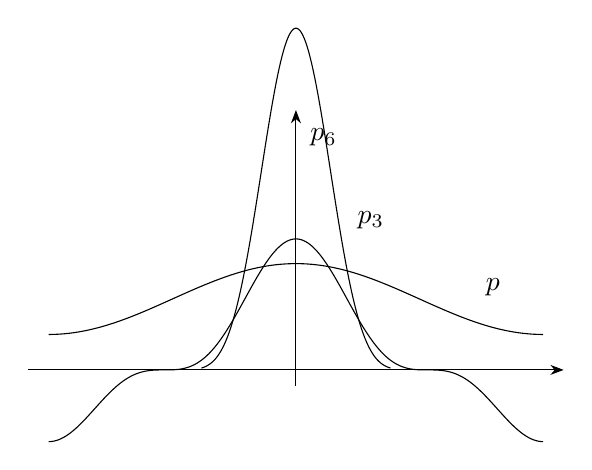
\begin{tikzpicture}[scale=1.0,>=Stealth]
			\draw[->] (-3.4,0) -- (3.4,0);
			\draw[->] (0,-0.2) -- (0,3.3);
			\draw[domain=-3.14:3.14,samples=200,smooth] plot (\x,{0.9+0.45*cos(\x r)});
			\draw[domain=-3.14:3.14,samples=300,smooth] plot (\x,{1.25*(0.1+cos(\x r))^3});
			\draw[domain=-1.2:1.2,samples=300,smooth] plot (\x,{2.45*(0.1+cos(\x r))^6});
			\node at (2.5,1.05) {$p$};
			\node at (0.95,1.9) {$p_3$};
			\node at (0.35,2.95) {$p_{6}$};
		\end{tikzpicture}
	\end{center}
	
	一般地,令
	\[
	f(\theta)=u(\theta)+iv(\theta),
	\]
	其中 $u$ 和 $v$ 是实值函数。若定义 $\overline f(\theta)=\overline{f(\theta)}$,那么有
	\[
	u(\theta)=\frac{f(\theta)+\overline f(\theta)}2,
	\qquad
	v(\theta)=\frac{f(\theta)-\overline f(\theta)}{2i}.
	\]
	又因为$\widehat{\overline f}(n)=\overline{\widehat f(-n)},$

	所以 $u$ 和 $v$ 的 Fourier 系数也全为零。由实值情形可得,在 $f$ 的连续点有
	\[
	u(\theta_0)=0,
	\qquad
	v(\theta_0)=0.
	\]
	因此 $f(\theta_0)=0$。
	
\end{proof}

根据上面的命题不难得到以下的命题
\begin{corollary}
	如果 $f$ 在圆周上连续且对所有 $n\in\Z$,有$\widehat f(n)=0,$则$f=0.$
	
\end{corollary}
\begin{corollary}
	如果 $f,g$ 在圆周上连续且对所有 $n\in\Z$,有$\widehat f(n)=\widehat g(n),$则$f=g.$
	
\end{corollary}
这也就是所谓的Fourier级数的唯一性

\begin{corollary}
	假设 $f$ 是在圆周上的连续函数且 $f$ 的 Fourier 系数绝对收敛,即
	\[
	\sum_{n=-\infty}^{\infty}|\widehat f(n)|<\infty.
	\]
	那么,$f$ 的 Fourier 级数一致收敛于 $f$,即
	\[
	\lim_{N\to\infty}S_N(f)(\theta)=f(\theta),
	\]
	且上述收敛关于 $\theta$ 是一致的。
\end{corollary}

\begin{proof}
由
	\[
	\sum_{n=-\infty}^{\infty}|\widehat f(n)|<\infty
	\]
	可知,$f$ 的 Fourier 系数的部分和绝对且一致收敛。事实上,由 Weierstrass $M$ 判别法,级数
	\[
	\sum_{n=-\infty}^{\infty}|\widehat f(n)e^{in\theta}| =\sum_{n=-\infty}^{\infty}|\widehat f(n)|<\infty
	\]
	在圆周上一致收敛。于是可以定义
	\[
	g(\theta)=\sum_{n=-\infty}^{\infty}\widehat f(n)e^{in\theta}
	=\lim_{N\to\infty}\sum_{n=-N}^{N}\widehat f(n)e^{in\theta}.
	\]
	由一致收敛和每一项的连续性可知,$g$ 在圆周上连续。
	
	进一步,由一致收敛可以交换无穷求和与积分,所以 $g$ 的 Fourier 系数恰好是 $\widehat f(n)$。具体地,
	\[
	\begin{aligned}
		\widehat g(n)
		&=\frac1{2\pi}\int_{-\pi}^{\pi}g(\theta)e^{-in\theta}\dd\theta                         \\
		&=\frac1{2\pi}\int_{-\pi}^{\pi}\sum_{m=-\infty}^{\infty}
		\widehat f(m)e^{im\theta}e^{-in\theta}\dd\theta                                             \\
		&=\frac1{2\pi}\sum_{m=-\infty}^{\infty}\widehat f(m)
		\int_{-\pi}^{\pi}e^{i(m-n)\theta}\dd\theta                                                   \\
		&=\widehat f(n).
	\end{aligned}
	\]
	因此 $f-g$ 的所有 Fourier 系数均为零。由上一推论,$f-g=0$,于是 $f=g$。也就是说,$f$ 的 Fourier 级数一致收敛于 $f$。
\end{proof}

\begin{corollary}\label{f(n)=O(1/n2)}
	假设 $f$ 是定义在圆周上的二次连续可微函数。当 $|n|\to\infty$ 时,有
	\[
	\widehat f(n)=O\left(\frac1{|n|^2}\right).
	\]
	则 $f$ 的 Fourier 级数绝对收敛且一致收敛于 $f$。
\end{corollary}

\begin{proof}
	当 $n\neq0$ 时,计算 Fourier 系数需要使用两次分部积分。取周期区间 $[0,2\pi]$,有
	\[
	\begin{aligned}
		2\pi\widehat f(n)
		&=\int_0^{2\pi}f(\theta)e^{-in\theta}\dd\theta                                      \\
		&=\left[f(\theta)\cdot \left(-\frac{e^{-in\theta}}{in}\right)\right]_0^{2\pi}
		+\frac1{in}\int_0^{2\pi}f'(\theta)e^{-in\theta}\dd\theta                              \\
		&=\frac1{in}\int_0^{2\pi}f'(\theta)e^{-in\theta}\dd\theta                              \\
		&=\frac1{in}\left[f'(\theta)\cdot\left(-\frac{e^{-in\theta}}{in}\right)\right]_0^{2\pi}
		+\frac1{(in)^2}\int_0^{2\pi}f''(\theta)e^{-in\theta}\dd\theta                          \\
		&=-\frac1{n^2}\int_0^{2\pi}f''(\theta)e^{-in\theta}\dd\theta.
	\end{aligned}
	\]
	由于 $f$ 和 $f'$ 是周期的,所以括号中的边界项均为零。因此
	\[
	2\pi |n|^2|\widehat f(n)|
	\leq \int_0^{2\pi}|f''(\theta)|\dd\theta
	\leq C,
	\]
	其中 $C$ 是与 $n$ 无关的常数。因为 $\sum 1/n^2$ 收敛,所以
	\[
	\sum_{n=-\infty}^{\infty}|\widehat f(n)|<\infty.
	\]
	由上一推论,$f$ 的 Fourier 级数绝对收敛且一致收敛于 $f$。
\end{proof}
进一步的,我们提高$f$的光滑性,得
\begin{corollary}\label{f(n)=O(1/n^k)}
	假设 $f\in C^k(\mathbb T)$,其中 $k\geq 1$。则当 $|n|\to\infty$ 时,
	\[
	\widehat f(n)=O\left(\frac1{|n|^k}\right).
	\]
	特别地,当 $k\geq 2$ 时,$f$ 的 Fourier 级数绝对收敛且一致收敛于 $f$。
\end{corollary}

我们还建立了以下重要等式：
\[
\widehat{f'}(n)=in\widehat f(n),
\qquad \forall n\in\Z.
\]
如果 $n\neq0$,这已经包含在上面的分部积分计算中；当 $n=0$ 时,
\[
\widehat{f'}(0)
=\frac1{2\pi}\int_0^{2\pi}f'(\theta)\dd\theta
=\frac{f(2\pi)-f(0)}{2\pi}=0=i0\widehat f(0),
\]
其中使用了 $f$ 的周期性。因此,如果 $f$ 是可微的且
\[
f\sim\sum a_ne^{in\theta},
\]
那么
\[
f'\sim\sum a_n in e^{in\theta}.
\]
同样,若 $f$ 是二次连续可微的,那么
\[
f''\sim\sum a_n(in)^2e^{in\theta}.
\]
在 $f$ 上附加更好的光滑性表现为 Fourier 系数衰减更迅速。
%
% 第3节：卷积
% !TEX root = ../../../main.tex
% 所属：第四部分：Fourier 分析 / 第1章：Fourier级数的基本性质
% 节：1.3 卷积
% 正文按原文件顺序保存；由 ../chapter1.tex 调用。
\section{卷积}
考虑\[
\begin{aligned}
	S_N(f)(x)
	&=\sum_{n=-N}^{N}\widehat f(n)e^{inx} \\
	&=\sum_{n=-N}^{N}\left(\frac1{2\pi}\int_{-\pi}^{\pi}f(y)e^{-iny}\dd y\right)e^{inx} \\
	&=\frac1{2\pi}\int_{-\pi}^{\pi}f(y)\left(\sum_{n=-N}^{N}e^{in(x-y)}\right)\dd y \\
\end{aligned}
\]
回忆$N$ 次 Dirichlet 核$D_N$ ,即
\[
D_N(x)=\sum_{n=-N}^{N}e^{inx}.
\]
可以给出以下的定义
\begin{definition}
	
给定两个在 $\R$ 上的、以 $2\pi$ 为周期的可积函数 $f$ 和 $g$,定义它们在 $[-\pi,\pi]$ 上的卷积为

	\[(f\ast g)(x)=\frac1{2\pi}\int_{-\pi}^{\pi}f(y)g(x-y)\dd y .\]

\end{definition}
因为两个可积函数的乘积也是可积的,故上面的积分对任意的 $x$ 都有意义。同样,由于函数具有周期性,通过改变变量可得
\[
(f\ast g)(x)=\frac1{2\pi}\int_{-\pi}^{\pi}f(x-y)g(y)\dd y .
\]

那么\[S_N(f)(x)=f\ast D_N(x)\]

因此,理解 $S_N(f)$ 的问题就简化为对卷积 $f\ast D_N$ 的理解。

\begin{proposition}
	假设 $f,g,h$ 是以 $2\pi$ 为周期的可积函数,则有：
	\[
	\begin{array}{ll}
		\mathrm{(i)}  & f\ast(g+h)=(f\ast g)+(f\ast h),\\[2mm]
		\mathrm{(ii)} & (cf)\ast g=c(f\ast g)=f\ast(cg),\quad \forall c\in\C,\\[2mm]
		\mathrm{(iii)}& f\ast g=g\ast f,\\[2mm]
		\mathrm{(iv)} & (f\ast g)\ast h=f\ast(g\ast h),\\[2mm]
		\mathrm{(v)}  & f\ast g \text{ 是连续的},\\[2mm]
		\mathrm{(vi)} & \widehat{f\ast g}(n)=\widehat f(n)\widehat g(n),\quad n\in\Z.
	\end{array}
	\]
\end{proposition}
前四点描述的是卷积的代数性质：线性性、交换性、结合性。性质 $\mathrm{(v)}$ 展示了一个重要原则：卷积具有平滑效果。这就是说,即使 $f$ 和 $g$ 只是 Riemann 可积的,$f\ast g$ 也是连续函数。最后 $\mathrm{(vi)}$ 是研究 Fourier 系数的关键,它说明卷积的 Fourier 系数等于 Fourier 系数的乘积。
\begin{proof}
	性质 $\mathrm{(i)}$ 和 $\mathrm{(ii)}$ 由积分的线性性立即得到。先假设 $f$ 和 $g$ 都是连续函数,则可以自由交换积分顺序(实际上在这一个问题中,仅仅有可积性,就可以交换积分次序)。对于性质 $\mathrm{(vi)}$,有
	\[
	\begin{aligned}
		\widehat{f\ast g}(n)
		&=\frac1{2\pi}\int_{-\pi}^{\pi}(f\ast g)(x)e^{-inx}\dd x \\
		&=\frac1{2\pi}\int_{-\pi}^{\pi}
		\left(\frac1{2\pi}\int_{-\pi}^{\pi}f(y)g(x-y)\dd y\right)e^{-inx}\dd x \\
		&=\frac1{2\pi}\int_{-\pi}^{\pi}f(y)e^{-iny}
		\left(\frac1{2\pi}\int_{-\pi}^{\pi}g(x-y)e^{-in(x-y)}\dd x\right)\dd y \\
		&=\frac1{2\pi}\int_{-\pi}^{\pi}f(y)e^{-iny}\widehat g(n)\dd y \\
		&=\widehat f(n)\widehat g(n).
	\end{aligned}
	\]
	
	为了证明性质 $\mathrm{(iii)}$,注意到如果 $F$ 是以 $2\pi$ 为周期的连续函数,则对任意 $x\in\R$,
	\[
	\int_{-\pi}^{\pi}F(y)\dd y
	=\int_{-\pi}^{\pi}F(x-y)\dd y.
	\]
	于是由变量替换可得
	\[
	(f\ast g)(x)=\frac1{2\pi}\int_{-\pi}^{\pi}f(x-y)g(y)\dd y=(g\ast f)(x).
	\]
	同样,性质 $\mathrm{(iv)}$ 在交换两个积分符号并作适当变量变换后得到。
	
	最后证明连续性。若 $f$ 和 $g$ 都连续,则 $g$ 在圆周上一致连续。任取 $\eps>0$,存在 $\delta>0$,使得当 $|s-t|<\delta$ 时,
	\[
	|g(s)-g(t)|<\eps.
	\]
	若 $|x_1-x_2|<\delta$,则对任意 $y$,有
	\[
	|(x_1-y)-(x_2-y)|<\delta.
	\]
	故
	\[
	\begin{aligned}
		|(f\ast g)(x_1)-(f\ast g)(x_2)|
		&\leq \frac1{2\pi}\int_{-\pi}^{\pi}|f(y)|\,|g(x_1-y)-g(x_2-y)|\dd y \\
		&\leq \frac{\eps}{2\pi}\int_{-\pi}^{\pi}|f(y)|\dd y.
	\end{aligned}
	\]
	于是 $f\ast g$ 是连续的。
	
	一般情况下,当 $f$ 和 $g$ 仅仅是可积函数时,需要用连续函数来逼近它们。\ref{C在R中一致有界稠密}给出这一点。

	对 $f$ 和 $g$ 应用\ref{C在R中一致有界稠密},得到近似的连续函数列 $\{f_k\}$ 和 $\{g_k\}$。于是
	\[
	f\ast g-f_k\ast g_k=(f-f_k)\ast g+f_k\ast(g-g_k).
	\]
	由引理的性质,当 $k\to\infty$ 时,
	\[
	\begin{aligned}
		|(f-f_k)\ast g(x)|
		&\leq \frac1{2\pi}\int_{-\pi}^{\pi}|f(x-y)-f_k(x-y)|\,|g(y)|\dd y \\
		&\leq \frac1{2\pi}\sup_y|g(y)|\int_{-\pi}^{\pi}|f(y)-f_k(y)|\dd y
		\to0.
	\end{aligned}
	\]
	所以 $(f-f_k)\ast g$ 关于 $x$ 一致收敛到 $0$。同理,$f_k\ast(g-g_k)$ 也一致收敛到 $0$。因此
	\[
	f_k\ast g_k\to f\ast g
	\]
	一致收敛。因为每个 $f_k\ast g_k$ 都是连续函数,故 $f\ast g$ 也是连续函数,从而得到了性质 $\mathrm{(v)}$。
	
	接下来证明性质 $\mathrm{(vi)}$。对每个固定的 $n$,由 $f_k\ast g_k$ 一致收敛于 $f\ast g$,得到
	\[
	\widehat{f_k\ast g_k}(n)\to\widehat{f\ast g}(n).
	\]
	另一方面,连续情形已经证明
	\[
	\widehat{f_k\ast g_k}(n)=\widehat f_k(n)\widehat g_k(n).
	\]
	并且
	\[
	|\widehat f(n)-\widehat f_k(n)|
	\leq \frac1{2\pi}\int_{-\pi}^{\pi}|f(x)-f_k(x)|\dd x\to0,
	\]
	类似地,$\widehat g_k(n)\to\widehat g(n)$。令 $k\to\infty$,便得到
	\[
	\widehat{f\ast g}(n)=\widehat f(n)\widehat g(n).
	\]
	最后,性质 $\mathrm{(iii)}$ 和性质 $\mathrm{(iv)}$ 也可以由连续函数情形再通过上述逼近过程得到。
\end{proof}

%
% 第4节：好核
% !TEX root = ../../../main.tex
% 所属：第四部分：Fourier 分析 / 第1章：Fourier级数的基本性质
% 节：1.4 好核
% 正文按原文件顺序保存；由 ../chapter1.tex 调用。
\section{好核}

卷积可以看成一种加权平均。若 $K_n$ 是以 $2\pi$ 为周期的函数,则
\[
(f\ast K_n)(x)=\frac1{2\pi}\int_{-\pi}^{\pi}f(x-y)K_n(y)\dd y.
\]
$K_n$起到了加权的作用,称做卷积核

\begin{definition}
	定义在圆周上的一列函数 $\{K_n(x)\}_{n=1}^{\infty}$ 满足以下性质：
	\[
	\begin{array}{ll}
		\mathrm{(a)} & \displaystyle \frac1{2\pi}\int_{-\pi}^{\pi}K_n(x)\dd x=1,\qquad n\geq1,\\[4mm]
		\mathrm{(b)} & \displaystyle \text{存在 }M>0,\text{ 对所有 }n\geq1,\text{ 有 }
		\int_{-\pi}^{\pi}|K_n(x)|\dd x\leq M,\\[4mm]
		\mathrm{(c)} & \displaystyle \text{对每一个 }\delta>0,\text{ 当 }n\to\infty\text{ 时,}
		\int_{\delta\leq |x|\leq\pi}|K_n(x)|\dd x\to0.
	\end{array}
	\]
	则称 $\{K_n(x)\}_{n=1}^{\infty}$ 为好核。
\end{definition}

\begin{theorem}
	假设 $\{K_n(x)\}_{n=1}^{\infty}$ 是好核列,且 $f$ 是圆周上的可积函数,则
	\[
	\lim_{n\to\infty}(f\ast K_n)(x)=f(x),
	\]
	其中 $f$ 在点 $x$ 连续。如果 $f$ 处处连续,那么上面的极限是一致收敛的。
\end{theorem}

\begin{proof}
	假设 $f$ 在点 $x$ 连续。给定 $\eps>0$,由连续性,选取 $\delta>0$,使得当 $|y|<\delta$ 时,有
	\[
	|f(x-y)-f(x)|<\eps.
	\]
	由好核的第一个性质,有
	\[
	\begin{aligned}
		(f\ast K_n)(x)-f(x)
		&=\frac1{2\pi}\int_{-\pi}^{\pi}K_n(y)f(x-y)\dd y-f(x) \\
		&=\frac1{2\pi}\int_{-\pi}^{\pi}K_n(y)[f(x-y)-f(x)]\dd y.
	\end{aligned}
	\]
	因此
	\[
	\begin{aligned}
		|(f\ast K_n)(x)-f(x)|
		&\leq \frac1{2\pi}\int_{|y|<\delta}|K_n(y)|\,|f(x-y)-f(x)|\dd y \\
		&\quad +\frac1{2\pi}\int_{\delta\leq |y|\leq\pi}|K_n(y)|\,|f(x-y)-f(x)|\dd y \\
		&\leq \frac{\eps}{2\pi}\int_{-\pi}^{\pi}|K_n(y)|\dd y
		+\frac{2B}{2\pi}\int_{\delta\leq |y|\leq\pi}|K_n(y)|\dd y,
	\end{aligned}
	\]
	其中 $B$ 是 $f$ 的界。由于好核的第二个性质,第一项被 $\eps M/(2\pi)$ 控制；由于好核的第三个性质,当 $n$ 足够大时,第二项可以任意小。因此存在常数 $C>0$,使得对充分大的 $n$,
	\[
	|(f\ast K_n)(x)-f(x)|<C\eps.
	\]
	这就证明了 $(f\ast K_n)(x)\to f(x)$。
	
	如果 $f$ 处处连续,则 $f$ 在圆周上一致连续,所以上面 $\delta$ 的选取可以独立于 $x$。于是上述估计对所有 $x$ 同时成立,从而得到一致收敛。
\end{proof}

%
% 第5节：Ces\`aro 和 Abel 求和：Fourier 级数的应用
% !TEX root = ../../../main.tex
% 所属：第四部分：Fourier 分析 / 第1章：Fourier级数的基本性质
% 节：1.5 Ces\`aro 和 Abel 求和：Fourier 级数的应用
% 正文按原文件顺序保存；由 ../chapter1.tex 调用。
\section{Ces\`aro 和 Abel 求和：Fourier 级数的应用}

因为 Fourier 级数可能在个别点处发散,为了克服这种缺点,我们寻求通过另一种方式来表示极限
\[
\lim_{N\to\infty}S_N(f)=f.
\]

假定给出一个复数级数
\[
c_0+c_1+c_2+\cdots=\sum_{k=0}^{\infty}c_k.
\]
定义第 $n$ 项和 $s_n$ 为
\[
s_n=\sum_{k=0}^{n}c_k.
\]
\begin{definition}
	我们定义前 $N$ 项和的平均值
\[
\sigma_N=\frac{s_0+s_1+\cdots+s_{N-1}}{N}
\]

量 $\sigma_N$ 被称为级数 $\{s_n\}$ 的 $N$ 次 Ces\`aro 平均,或级数 $\sum\limits_{k=0}^{\infty}c_k$ 的 $N$ 次 Ces\`aro 和。如果当 $N$ 趋于无穷时,$\sigma_N$ 收敛于一个极限 $s$,我们就说级数是 Ces\`aro 可和的,并称 $s$ 为它的 Ces\`aro 和。在函数级数的情形下,我们关心的是级数是逐点收敛的还是一致收敛的。

\end{definition}
我们早先提及 Dirichlet 核不属于好核的类。但它们的平均是性质很好的核。我们用对 Fourier 级数的 $N$ 次 Ces\`aro 和,具体定义如下：
\begin{definition}
	\[
\sigma_N(f)(x)=\frac{S_0(f)(x)+\cdots+S_{N-1}(f)(x)}{N}.
\]
因为 $S_N(f)=f\ast D_N$,故有
\[
\sigma_N(f)(x)=(f\ast F_N)(x),
\]
其中 $F_N(x)$ 是 $N$ 次 Fej\'er 核,定义如下：
\[
F_N(x)=\frac{D_0(x)+\cdots+D_{N-1}(x)}{N}=\sum_{\abs{k}\leqslant N}(1-\frac{|k|}{N})e^{ikx}.
\]
\end{definition}

\begin{lemma}
	可以得到
	\[
	F_N(x)=\frac1N\frac{\sin^2(Nx/2)}{\sin^2(x/2)},
	\]
	且 Fej\'er 核是好核。
\end{lemma}

\begin{proof}
	由定义,
	\[
	\begin{aligned}
		F_N(x)
		&=\frac1N\sum_{k=0}^{N-1}D_k(x)
		=\frac1N\sum_{k=0}^{N-1}\sum_{n=-k}^{k}e^{inx} \\
		&=\frac1N\sum_{|n|\leq N-1}(N-|n|)e^{inx}.
	\end{aligned}
	\]
	另一方面,
	\[
	\begin{aligned}
		\left|\sum_{j=0}^{N-1}e^{ijx}\right|^2
		&=\left(\sum_{j=0}^{N-1}e^{ijx}\right)
		\left(\sum_{k=0}^{N-1}e^{-ikx}\right) \\
		&=\sum_{|n|\leq N-1}(N-|n|)e^{inx}.
	\end{aligned}
	\]
	于是
	\[
	F_N(x)=\frac1N\left|\sum_{j=0}^{N-1}e^{ijx}\right|^2
	=\frac1N\left|\frac{1-e^{iNx}}{1-e^{ix}}\right|^2
	=\frac1N\frac{\sin^2(Nx/2)}{\sin^2(x/2)}.
	\]
	由上式可见 $F_N(x)\geq0$。又因为 $F_N$ 的第 $0$ 个 Fourier 系数为 $1$,所以
	\[
	\frac1{2\pi}\int_{-\pi}^{\pi}F_N(x)\dd x=1.
	\]
	因此
	\[
	\int_{-\pi}^{\pi}|F_N(x)|\dd x=\int_{-\pi}^{\pi}F_N(x)\dd x=2\pi.
	\]
	最后,给定 $\delta>0$,当 $\delta\leq |x|\leq\pi$ 时,$\sin^2(x/2)$ 有正的下界,于是
	\[
	0\leq F_N(x)\leq \frac{C_\delta}{N}.
	\]
	故
	\[
	\int_{\delta\leq |x|\leq\pi}F_N(x)\dd x\to0.
	\]
	所以 $\{F_N\}$ 是好核。
\end{proof}

\begin{theorem}
	如果 $f$ 在圆周上可积,那么 $f$ 的 Fourier 级数在 $f$ 的每个连续点是 Ces\`aro 和于 $f$ 的。并且,如果 $f$ 在圆周上连续,那么 $f$ 的 Fourier 级数是一致 Ces\`aro 和于 $f$ 的。
\end{theorem}

\begin{proof}
	由上一引理,$F_N$ 是好核。又因为
	\[
	\sigma_N(f)(x)=(f\ast F_N)(x),
	\]
	所以由好核逼近定理立即得到结论。
\end{proof}

\begin{corollary}
	若 $f$ 在圆周上可积且对所有 $n$,有 $\widehat f(n)=0$,则在 $f$ 的所有连续点都有
	\[
	f=0.
	\]
\end{corollary}

\begin{proof}
	这显然是成立的。因为 $f$ 的所有部分和都是零,所以其 Ces\`aro 平均也是零。由上一定理,在 $f$ 的连续点处,Ces\`aro 平均收敛到 $f$,于是 $f=0$。
\end{proof}

\begin{corollary}
	圆周上的连续函数可以被三角多项式一致逼近。更精确地说,给定任意 $\eps>0$,存在三角多项式 $P$,使得对任意的 $-\pi\leq x\leq\pi$,
	\[
	|f(x)-P(x)|<\eps
	\]
	成立。
\end{corollary}

\begin{proof}
	由于 Fourier 部分和是三角多项式,所以 Ces\`aro 平均 $\sigma_N(f)$ 也是三角多项式,从而直接由上一定理的一致收敛性得到结论。这个结论就是周期函数的 Weierstrass 逼近定理。
\end{proof}

\begin{definition}
	如果对任意的 $0<r<1$,级数
\[
A(r)=\sum_{k=0}^{\infty}c_k r^k
\]
收敛,且
\[
\lim_{r\to1}A(r)=s,
\]
则复数 $s$ 称为级数 $\sum\limits_{k=0}^{\infty}c_k$ 的 Abel 求和,$A(r)$ 称为此级数的 Abel 平均。如果这个级数收敛于 $s$,那么它是 Abel 和于 $s$
\end{definition}
 另外,Abel 和方法甚至比 Ces\`aro 方法更强。也就是说,当级数是 Ces\`aro 和时,它也是 Abel 和于相同的数。然而,如果考虑级数
\[
1-2+3-4+5-\cdots=\sum_{k=0}^{\infty}(-1)^k(k+1),
\]
由于
\[
A(r)=\sum_{k=0}^{\infty}(-1)^k(k+1)r^k=\frac1{(1+r)^2},
\]
故可以证明它是 Abel 和于 $1/4$,但这个级数不是 Ces\`aro 和的。
\begin{proposition}
	Abel 求和要比一般求和以及 Ces\`aro 求和更强,具体如下
	
	\begin{enumerate}
		\item[(a)] 若复数级数$\sum\limits_{n=1}^{\infty}c_n$
		收敛于一个有限数 $s$,则它的 Abel 和为 $s$
		\item[(b)] 存在 Abel 可求和但是不收敛的级数。
		\item[(c)] 类似地,证明：若$\sum\limits_{n=1}^{\infty}c_n$的 Ces\`aro 和为 $\sigma$,则它的 Abel 和也为 $\sigma$。
		\item[(d)] 给出一个有 Abel 和,但是 Ces\`aro 和发散的例子。
	\end{enumerate}
	这些结果可以总结为
	\[
	\text{收敛}
	\Longrightarrow
	\text{Ces\`aro 可求和}
	\Longrightarrow
	\text{Abel 可求和},
	\]
	其中的箭头均无法逆向成立。
\end{proposition}

\begin{solution}
	\textbf{(a)}
	
	
	先假设$ \sum\limits_{n=1}^{\infty}c_n=0.$令$s_N=\sum\limits_{n=1}^{N}c_n,$则 $s_N\to0$,从而数列 $\{s_N\}$ 有界。
	
	注意到
	\[
	c_n=s_n-s_{n-1},
	\qquad s_0=0,
	\]
	所以
	\[\sum_{n=1}^{N}c_nr^n
	=\sum_{n=1}^{N}(s_n-s_{n-1})r^n
	=\sum_{n=1}^{N}s_nr^n
	-r\sum_{n=1}^{N-1}s_nr^n
	=(1-r)\sum_{n=1}^{N}s_nr^n+s_Nr^{N+1}
	\]
	
	固定 $0<r<1$。由于 $\{s_N\}$ 有界,
	\[
	s_Nr^{N+1}\to0.
	\]
	令 $N\to\infty$,得到
	\[
	\sum_{n=1}^{\infty}c_nr^n
	=(1-r)\sum_{n=1}^{\infty}s_nr^n.
	\]
	
	下面证明右端在 $r\to1^-$ 时趋于 $0$。给定 $\varepsilon>0$,由 $s_n\to0$,存在正整数 $N_0$,使得当 $n>N_0$ 时,
	\[
	|s_n|<\varepsilon.
	\]
	于是
	\[
	\begin{aligned}
		(1-r)\left|\sum_{n=1}^{\infty}s_nr^n\right|
		&\leq
		(1-r)\sum_{n=1}^{N_0}|s_n|r^n
		+(1-r)\sum_{n=N_0+1}^{\infty}|s_n|r^n\\
		&\leq
		(1-r)\sum_{n=1}^{N_0}|s_n|r^n
		+\varepsilon(1-r)\sum_{n=N_0+1}^{\infty}r^n.
	\end{aligned}
	\]
	当 $r\to1^-$ 时,第一项趋于 $0$,而第二项满足
	\[
	\varepsilon(1-r)\sum_{n=N_0+1}^{\infty}r^n
	=\varepsilon r^{N_0+1}
	\leq\varepsilon.
	\]
	因此
	\[
	\lim_{r\to1^-}(1-r)\sum_{n=1}^{\infty}s_nr^n=0.
	\]
	所以
	\[
	\lim_{r\to1^-}\sum_{n=1}^{\infty}c_nr^n=0.
	\]
	
	综上,若
	\[
	\sum_{n=1}^{\infty}c_n=s,
	\]
	则该级数的 Abel 和也是 $s$。
	再说明为什么只需考虑 $s=0$ 的情形。若
	\[
	\sum_{n=1}^{\infty}c_n=s,
	\]
	定义
	\[
	d_1=c_1-s,\qquad d_n=c_n\quad(n\geq2).
	\]
	则
	\[
	\sum_{n=1}^{\infty}d_n=0,
	\]
	并且
	\[
	\sum_{n=1}^{\infty}c_nr^n
	=\sum_{n=1}^{\infty}d_nr^n+sr.
	\]
	因此,只要证明和为 $0$ 的收敛级数的 Abel 和为 $0$,便有
	\[
	\lim_{r\to1^-}\sum_{n=1}^{\infty}c_nr^n
	=0+s=s.
	\]
	
	\textbf{(b)}取	$c_n=(-1)^n.$相应的级数为$-1+1-1+1-\cdots.$其部分和满足
	\[
	s_{2m}=0,\qquad s_{2m-1}=-1,
	\]
	因此该级数不收敛。
	
	但是,当 $0<r<1$ 时,
	\[	\sum_{n=1}^{\infty}c_nr^n
	=\sum_{n=1}^{\infty}(-1)^nr^n
	=-r+r^2-r^3+\cdots
	=-\frac{r}{1+r}.
	\]
	所以
	\[
	\lim_{r\to1^-}\sum_{n=1}^{\infty}c_nr^n
	=-\frac12.
	\]
	因此该级数虽然不收敛,却是 Abel 可求和的,且 Abel 和为$-\frac12.$
	
	事实上,该级数也是 Ces\`aro 可求和的。因为
	\[
	\sigma_N=\frac{s_1+\cdots+s_N}{N},
	\]
	所以
	\[
	\sigma_{2m}
	=\frac{-m}{2m}
	=-\frac12,
	\]
	而
	\[
	\sigma_{2m-1}
	=\frac{-m}{2m-1}
	\to-\frac12.
	\]
	故其 Ces\`aro 和也为 $-\dfrac12$。
	
	\textbf{(c)}设
	\[
	s_n=c_1+\cdots+c_n,
	\qquad
	\sigma_n=\frac{s_1+\cdots+s_n}{n},
	\]
	并假设$\sigma_n\to\sigma.$
	
	类似于第 (a) 问,只需考虑 $\sigma=0$ 的情形。事实上,若定义
	\[
	d_1=c_1-\sigma,\qquad d_n=c_n\quad(n\geq2),
	\]
	则新级数的部分和为$t_n=s_n-\sigma,$其 Ces\`aro 平均为
	\[
	\frac{t_1+\cdots+t_n}{n}
	=\sigma_n-\sigma\to0.
	\]
	同时
	\[
	\sum_{n=1}^{\infty}c_nr^n
	=\sum_{n=1}^{\infty}d_nr^n+\sigma r.
	\]
	因此只需证明 Ces\`aro 和为 $0$ 时,Abel 和也为 $0$。
	
	下面假设$\sigma_n\to0.$由$n\sigma_n=s_1+\cdots+s_n$可得
	\[
	s_n=n\sigma_n-(n-1)\sigma_{n-1},
	\]
	其中规定 $\sigma_0=0$。
	
	于是
	\[\sum_{n=1}^{\infty}s_nr^n
	=\sum_{n=1}^{\infty}
	\bigl(n\sigma_n-(n-1)\sigma_{n-1}\bigr)r^n
	=\sum_{n=1}^{\infty}n\sigma_nr^n
	-r\sum_{n=1}^{\infty}n\sigma_nr^n
	=(1-r)\sum_{n=1}^{\infty}n\sigma_nr^n.
	\]
	由第 (a) 问中的分部求和公式,
	\[
	\sum_{n=1}^{\infty}c_nr^n
	=(1-r)\sum_{n=1}^{\infty}s_nr^n.
	\]
	因此
	\[
	\sum_{n=1}^{\infty}c_nr^n
	=(1-r)^2\sum_{n=1}^{\infty}n\sigma_nr^n.
	\]
	
	给定 $\varepsilon>0$,由 $\sigma_n\to0$,存在正整数 $N_0$,使得当 $n>N_0$ 时,
	\[
	|\sigma_n|<\varepsilon.
	\]
	于是
	\[(1-r)^2
	\left|\sum_{n=1}^{\infty}n\sigma_nr^n\right|
	\leq
	(1-r)^2\sum_{n=1}^{N_0}n|\sigma_n|r^n
	+
	\varepsilon(1-r)^2
	\sum_{n=N_0+1}^{\infty}nr^n.\]
	当 $r\to1^-$ 时,第一项趋于 $0$。又因为
	\[
	\sum_{n=1}^{\infty}nr^n=\frac{r}{(1-r)^2},
	\]
	所以第二项不超过
	\[
	\varepsilon(1-r)^2
	\sum_{n=1}^{\infty}nr^n
	=\varepsilon r
	\leq\varepsilon.
	\]
	故
	\[
	\lim_{r\to1^-}
	(1-r)^2\sum_{n=1}^{\infty}n\sigma_nr^n=0.
	\]
	
	因此,当 Ces\`aro 和为 $0$ 时,Abel 和也为 $0$。由前面的证明可知,若级数的 Ces\`aro 和为 $\sigma$,则其 Abel 和也是 $\sigma$。
	
	\textbf{(d)}取$c_n=(-1)^{n-1}n,$即考虑级数$	1-2+3-4+5-\cdots.$当 $0<r<1$ 时,由
	\[
	\sum_{n=0}^{\infty}(-r)^n=\frac{1}{1+r}
	\]
	两边对 $r$ 求导,得到
	\[
	\sum_{n=1}^{\infty}(-1)^{n-1}nr^{n-1}
	=\frac{1}{(1+r)^2}.
	\]
	两边乘以 $r$,得到
	\[
	\sum_{n=1}^{\infty}(-1)^{n-1}nr^n
	=\frac{r}{(1+r)^2}.
	\]
	因此
	\[
	\lim_{r\to1^-}
	\sum_{n=1}^{\infty}(-1)^{n-1}nr^n
	=\frac14.
	\]
	所以该级数是 Abel 可求和的,且 Abel 和为$\dfrac14.$
	
	
	下面证明它不是 Ces\`aro 可求和的。首先证明：若级数 $\sum c_n$ 是 Ces\`aro 可求和的,则$\dfrac{c_n}{n}\to0.$
	若 $\sigma_n\to\sigma$,则
	\[
	s_n=n\sigma_n-(n-1)\sigma_{n-1},
	\]
	从而
	\[
	\frac{s_n}{n}
	=\sigma_n-\frac{n-1}{n}\sigma_{n-1}
	\to\sigma-\sigma=0.
	\]
	又因为
	\[
	c_n=s_n-s_{n-1},
	\]
	所以
	\[
	\frac{c_n}{n}
	=\frac{s_n}{n}
	-\frac{n-1}{n}\frac{s_{n-1}}{n-1}
	\to0.
	\]
	
	但是对于$c_n=(-1)^{n-1}n,$有	$\dfrac{c_n}{n}=(-1)^{n-1},$
	
	它不趋于 $0$。因此级数$1-2+3-4+5-\cdots$不是 Ces\`aro 可求和的。
	
	综上,
	\[
	\boxed{
		\text{收敛}
		\Longrightarrow
		\text{Ces\`aro 可求和}
		\Longrightarrow
		\text{Abel 可求和}
	}
	\]
	且两个箭头均不能反向成立。
\end{solution}
下面介绍Tauber的一个定理,对上面的$c_n$
,添加一个条件后,上面的箭头就是可逆的
\begin{proposition}
	若$\sum c_n$的Ces\'aro和为$\sigma$,且$c_n = o(\dfrac{1}{n})$,则$\sum c_n$收敛与$\sigma$,对Abel和,有同样的结论
\end{proposition}
\begin{proof}
	考虑\[s_n- \sigma_n =\frac{(n-1)c_n +\cdots+c_2}{n}\]
	由$c_n = o(\dfrac{1}{n})$,$\forall \eps >0,\exists N_0,\text{使得}\forall n>N_0,c_n<\dfrac{\eps}{n}$
	那么
	\[s_n- \sigma_n =\frac{(n-1)c_n +\cdots+c_2}{n} =\frac{c_2+\cdots+(N_0-1)c_{N_0}}{n}+\frac{N_0 c_{N_0+1}\cdots+(n-1)c_n}{n}\]
	对第一项,存在$N>N_0$使,$\forall n>N$,$ \dfrac{c_2+\cdots+(N_0-1)c_{N_0}}{n}<\dfrac{\eps}{2}$对第二项
	\[\frac{N_0 c_{N_0+1}\cdots+(n-1)c_n}{n}<(1-\frac{N_0}{n})\frac{\eps}{2}\],因此
	\[s_n- \sigma_n< c\eps\]
	从而\[\lim\limits_{n\to \infty}s_n- \sigma_n =0\]
	对Abel和,类似的,我们考虑\[\sum_{n=1}^{N}c_n-\sum_{n=1}^{N}c_n r^n\]并且不妨取$r=1-\dfrac{1}{N}$
	\[\sum_{n=1}^{N}c_n-\sum_{n=1}^{N}c_n r^n<\sum_{n=1}^{N}c_n\frac{n}{N}\]类似于上面的方法,不难得出\[\sum_{n=1}^{N}c_n-\sum_{n=1}^{N}c_n r^n\to0\]
\end{proof}


\begin{definition}
	定义函数
\[
f(\theta)\sim\sum_{n=-\infty}^{\infty}a_ne^{in\theta}
\]
的 Abel 平均为
\[
A_r(f)(\theta)=\sum_{n=-\infty}^{\infty}r^{|n|}a_ne^{in\theta}.
\]
\end{definition}
因为指数 $n$ 取正值和负值,很自然地出现 $r^{|n|}$。并且当 $r>0$ 时,$c_n=a_ne^{in\theta}+a_{-n}e^{-in\theta}$,所以 Fourier 级数的 Abel 平均对应于普通级数的 Abel 平均的定义。

因为 $f$ 是可积的,$|a_n|$ 一致有界,所以对每个 $0\leq r<1$,$A_r(f)$ 绝对收敛且一致收敛。正如 Ces\`aro 平均的情形,关键是这些 Abel 平均可以写成卷积的形式,即
\[
A_r(f)(\theta)=(f\ast P_r)(\theta),
\]
其中 $P_r(\theta)$ 是 Poisson 核,定义如下：

	$$P_r(\theta)=\sum_{n=-\infty}^{\infty}r^{|n|}e^{in\theta}.$$

事实上,有
\[
\begin{aligned}
	A_r(f)(\theta)
	&=\sum_{n=-\infty}^{\infty}r^{|n|}a_ne^{in\theta} \\
	&=\sum_{n=-\infty}^{\infty}r^{|n|}
	\left(\frac1{2\pi}\int_{-\pi}^{\pi}f(\varphi)e^{-in\varphi}\dd\varphi\right)e^{in\theta} \\
	&=\frac1{2\pi}\int_{-\pi}^{\pi}f(\varphi)
	\left(\sum_{n=-\infty}^{\infty}r^{|n|}e^{in(\theta-\varphi)}\right)\dd\varphi,
\end{aligned}
\]
其中,交换积分和求和顺序是因为该级数一致收敛。

\begin{lemma}
	如果 $0\leq r<1$,那么有
	\[
	P_r(\theta)=\frac{1-r^2}{1-2r\cos\theta+r^2}.
	\]
	当 $r\to1$ 时,Poisson 核是好核。
\end{lemma}

\begin{proof}
	等式
	\[
	P_r(\theta)=\frac{1-r^2}{1-2r\cos\theta+r^2}
	\]
	已经在前面关于 Poisson 核的例子中给出。注意到由这个表达式可知 $P_r(\theta)>0$。此外,由于 $P_r$ 的第 $0$ 个 Fourier 系数为 $1$,得到
	\[
	\frac1{2\pi}\int_{-\pi}^{\pi}P_r(\theta)\dd\theta=1.
	\]
	因此
	\[
	\int_{-\pi}^{\pi}|P_r(\theta)|\dd\theta=2\pi.
	\]
	最后,给定 $\delta>0$。当 $1/2\leq r\leq1$ 且 $\delta\leq |\theta|\leq\pi$ 时,存在常数 $c_\delta>0$,使得
	\[
	1-2r\cos\theta+r^2\geq c_\delta.
	\]
	于是
	\[
	0\leq P_r(\theta)\leq \frac{1-r^2}{c_\delta}.
	\]
	当 $r\to1$ 时,上式右边趋于 $0$,故
	\[
	\int_{\delta\leq |\theta|\leq\pi}P_r(\theta)\dd\theta\to0.
	\]
	所以当 $r\to1$ 时,Poisson 核构成好核。
\end{proof}

\begin{theorem}
	在圆周上可积函数的 Fourier 级数在每个连续点 Abel 和于 $f$。此外,如果 $f$ 在圆周上连续,那么 $f$ 的 Fourier 级数一致 Abel 和于 $f$。
\end{theorem}

\begin{proof}
	由上一引理,$P_r$ 在 $r\to1$ 时构成好核。又因为
	\[
	A_r(f)(\theta)=(f\ast P_r)(\theta),
	\]
	所以由好核逼近定理可得结论。
\end{proof}
下面,我们考虑$f$在$\theta$处不连续的情况,我们只考虑跳跃点,即第一类间断点
\begin{proposition}

	\begin{enumerate}
		\item[(a)] 若 $f$ 在 $\theta$ 处是跃点,则
		\[
		\lim_{r\to1^-}A_r(f)(\theta)
		=\frac{f(\theta^+)+f(\theta^-)}{2}.
		\]
		
		\item[(b)] 类似的：若 $f$ 在 $\theta$ 处有跳跃间断,
		则 $f$ 在 $\theta$ 处的 Fourier 级数的 Ces\`aro 和为
		\[
		\frac{f(\theta^+)+f(\theta^-)}{2}.
		\]
	\end{enumerate}
	
\end{proposition}


\begin{proof}
	记
	\[
	\alpha=f(\theta^+),\qquad
	\beta=f(\theta^-),\qquad
	L=\frac{\alpha+\beta}{2}.
	\]
	
	\textbf{(a)}
	\[
	A_r(f)(\theta)
	=(P_r*f)(\theta)
	=\frac{1}{2\pi}\int_{-\pi}^{\pi}
	f(\theta-t)P_r(t)\dd t,
	\]
	其中 Poisson 核为
	\[
	P_r(t)=\frac{1-r^2}{1-2r\cos t+r^2}.
	\]
	
	由于 $P_r$ 是偶函数,且
	\[
	\frac{1}{2\pi}\int_{-\pi}^{\pi}P_r(t)\dd t=1,
	\]
	所以
	\[
	\frac{1}{2\pi}\int_{-\pi}^{0}P_r(t)\dd t
	=
	\frac{1}{2\pi}\int_{0}^{\pi}P_r(t)\dd t
	=\frac12.
	\]
	
	在积分区间 $[-\pi,0]$ 上作变量代换 $t\mapsto-t$,并利用
	$P_r(-t)=P_r(t)$,可得
	\[
	\begin{aligned}
		A_r(f)(\theta)
		&=\frac{1}{2\pi}\int_0^\pi
		f(\theta-t)P_r(t)\dd t
		+\frac{1}{2\pi}\int_0^\pi
		f(\theta+t)P_r(t)\dd t\\
		&=\frac{1}{2\pi}\int_0^\pi
		\bigl(f(\theta-t)+f(\theta+t)\bigr)P_r(t)\dd t.
	\end{aligned}
	\]
	
	另一方面,由
	\[
	\frac{1}{2\pi}\int_0^\pi P_r(t)\dd t=\frac12,
	\]
	有
	\[
	L
	=\frac{\alpha+\beta}{2}
	=\frac{1}{2\pi}\int_0^\pi
	(\alpha+\beta)P_r(t)\dd t.
	\]
	因此
	\[
	\begin{aligned}
		A_r(f)(\theta)-L
		&=\frac{1}{2\pi}\int_0^\pi
		\bigl[
		f(\theta+t)-\alpha
		+f(\theta-t)-\beta
		\bigr]P_r(t)\dd t.
	\end{aligned}
	\]
	
	给定 $\varepsilon>0$。由$\lim\limits_{\substack{t\to0\\t>0}}f(\theta+t)=\alpha,
	\lim\limits_{\substack{t\to0\\t>0}}f(\theta-t)=\beta,$
	存在 $\delta>0$,使得当 $0<t<\delta$ 时,
	\[
	|f(\theta+t)-\alpha|<\varepsilon,
	\qquad
	|f(\theta-t)-\beta|<\varepsilon.
	\]
	
	将积分分为 $(0,\delta)$ 和 $(\delta,\pi)$ 两部分。对于第一部分,
	由 $P_r(t)\geq0$,有
	\[\frac{1}{2\pi}\int_0^\delta
		\left|
		f(\theta+t)-\alpha
		+f(\theta-t)-\beta
		\right|P_r(t)\dd t\leq
		\frac{2\varepsilon}{2\pi}
		\int_0^\delta P_r(t)\dd t\leq
		\frac{2\varepsilon}{2\pi}
		\int_0^\pi P_r(t)\dd t
		=\varepsilon.
	\]
	
	对于第二部分,令
	\[
	C_\delta
	=
	\int_\delta^\pi
	\bigl(
	|f(\theta+t)|+|f(\theta-t)|+|\alpha|+|\beta|
	\bigr)\dd t.
	\]
	由于 $f$ 可积,故 $C_\delta<\infty$。于是
	\[\frac{1}{2\pi}\int_\delta^\pi
		\left|
		f(\theta+t)-\alpha
		+f(\theta-t)-\beta
		\right|P_r(t)\dd t\leq
		\frac{C_\delta}{2\pi}
		\sup_{\delta\leq t\leq\pi}P_r(t).\]
	
	当 $\delta\leq t\leq\pi$ 时,
	\[
	1-2r\cos t+r^2
	=(1-r)^2+2r(1-\cos t)
	\geq 2r(1-\cos\delta).
	\]
	因此,当 $r$ 充分接近 $1$ 时,
	\[
	P_r(t)
	\leq
	\frac{1-r^2}{2r(1-\cos\delta)},
	\qquad \delta\leq t\leq\pi.
	\]
	从而
	\[
	\sup_{\delta\leq t\leq\pi}P_r(t)\to0,
	\qquad r\to1^-.
	\]
	
	由此可得
	\[
	\limsup_{r\to1^-}|A_r(f)(\theta)-L|
	\leq\varepsilon.
	\]
	由于 $\varepsilon>0$ 任意,所以
	\[
	\lim_{r\to1^-}A_r(f)(\theta)
	=L
	=\frac{f(\theta^+)+f(\theta^-)}{2}.
	\]

	
	\textbf{(b)}
	由 Fej\'er 平均的卷积表示,
	\[
	\sigma_N(f)(\theta)
	=(F_N*f)(\theta)
	=\frac{1}{2\pi}\int_{-\pi}^{\pi}
	f(\theta-t)F_N(t)\dd t,
	\]
	其中 Fej\'er 核为
	\[
	F_N(t)
	=\frac{1}{N}
	\left(
	\frac{\sin(Nt/2)}{\sin(t/2)}
	\right)^2.
	\]
	
	Fej\'er 核具有下列性质：
	\[
	F_N(t)\geq0,\qquad F_N(-t)=F_N(t),
	\]
	并且
	\[
	\frac{1}{2\pi}\int_{-\pi}^{\pi}F_N(t)\dd t=1.
	\]
	因此
	\[
	\frac{1}{2\pi}\int_0^\pi F_N(t)\dd t=\frac12.
	\]
	
	与第 (a) 问相同,在负半区间作变量代换,得到
	\[
	\sigma_N(f)(\theta)
	=
	\frac{1}{2\pi}\int_0^\pi
	\bigl(f(\theta-t)+f(\theta+t)\bigr)F_N(t)\dd t.
	\]
	同时
	\[
	L
	=
	\frac{1}{2\pi}\int_0^\pi
	(\alpha+\beta)F_N(t)\dd t.
	\]
	所以
	\[
	\begin{aligned}
		\sigma_N(f)(\theta)-L
		&=\frac{1}{2\pi}\int_0^\pi
		\bigl[
		f(\theta+t)-\alpha
		+f(\theta-t)-\beta
		\bigr]F_N(t)\dd t.
	\end{aligned}
	\]
	
	给定 $\varepsilon>0$,取与第 (a) 问相同的 $\delta>0$,使得
	当 $0<t<\delta$ 时,
	\[
	|f(\theta+t)-\alpha|<\varepsilon,
	\qquad
	|f(\theta-t)-\beta|<\varepsilon.
	\]
	
	于是
	\[\frac{1}{2\pi}\int_0^\delta
		\left|
		f(\theta+t)-\alpha
		+f(\theta-t)-\beta
		\right|F_N(t)\dd t
		\leq
		\frac{2\varepsilon}{2\pi}
		\int_0^\delta F_N(t)\dd t\leq
		\frac{2\varepsilon}{2\pi}
		\int_0^\pi F_N(t)\dd t
		=\varepsilon.
	\]
	
	在 $\delta\leq t\leq\pi$ 上
	\[
	F_N(t)
	\leq
	\frac{1}{N\sin^2(\delta/2)}.
	\]
	因此
	\[
	\sup_{\delta\leq t\leq\pi}F_N(t)
	\leq
	\frac{1}{N\sin^2(\delta/2)}
	\to0,
	\qquad N\to\infty.
	\]
	
	利用第 (a) 问中定义的常数 $C_\delta$,有
	\[\frac{1}{2\pi}\int_\delta^\pi
		\left|
		f(\theta+t)-\alpha
		+f(\theta-t)-\beta
		\right|F_N(t)\dd t\leq
		\frac{C_\delta}{2\pi}
		\sup_{\delta\leq t\leq\pi}F_N(t)
		\to0.
	\]
	
	所以
	\[
	\limsup_{N\to\infty}
	|\sigma_N(f)(\theta)-L|
	\leq\varepsilon.
	\]
	由于 $\varepsilon>0$ 任意,得到
	\[
	\lim_{N\to\infty}\sigma_N(f)(\theta)
	=L
	=\frac{f(\theta^+)+f(\theta^-)}{2}.
	\]

\end{proof}
对上面的Tauber定理，Littlewood 给出了 一个细化版本
\begin{proposition}
	\begin{enumerate}
		\item[(a)] 若级数
		\[
		\sum_{n=1}^{\infty}c_n
		\]
		的 Abel 和为 $s$，且
		\[
		c_n=O\left(\frac{1}{n}\right),
		\]
		则
		\[
		\sum_{n=1}^{\infty}c_n
		\]
		在通常意义下收敛于 $s$。
		
		\item[(b)] 从而，若级数
		\[
		\sum_{n=1}^{\infty}c_n
		\]
		的 Ces\`aro 和为 $s$，且
		\[
		c_n=O\left(\frac{1}{n}\right),
		\]
		则
		\[
		\sum_{n=1}^{\infty}c_n
		\]
		在通常意义下收敛于 $s$。
	\end{enumerate}
\end{proposition}
证明极其复杂，这里略过

这些结果可以应用到 Fourier 级数上。若可积函数 $f$
满足
\[
\widehat{f}(\nu)
=O\left(\frac{1}{|\nu|}\right),
\qquad |\nu|\to\infty,
\]
则有：

\begin{enumerate}
	\item[(i)] 若 $f$ 在 $\theta$ 处连续，则当 $N\to\infty$ 时，
	\[
	S_N(f)(\theta)\to f(\theta).
	\]
	
	\item[(ii)] 若 $f$ 在 $\theta$ 处是跃点，则当 $N\to\infty$ 时，
	\[
	S_N(f)(\theta)
	\to
	\frac{f(\theta^+)+f(\theta^-)}{2}.
	\]
	
	\item[(iii)] 若 $f$ 在 $[-\pi,\pi]$ 上连续，则
	\[
	S_N(f)\rightrightarrows f.
	\]
\end{enumerate}
%

%% ===== 第四部分：Fourier 分析 / 第2章：Fourier级数的收敛性 =====
% !TEX root = ../../main.tex
\setchapterimage{figure/P4/P4C2封面图.png}
\setchapterintro{本章集中讨论 Fourier 级数在不同意义下的收敛问题。我们先研究均方收敛与逐点收敛，说明正交展开如何逼近原函数；随后构造连续函数的 Fourier 级数仍可能发散的反例，并在最后整理函数正则性与 Fourier 系数衰减速度之间的关系。}
\chapter{Fourier级数的收敛性}
% 第1节：Fourier级数的均方收敛
% !TEX root = ../../../main.tex
% 所属：第四部分：Fourier 分析 / 第2章：Fourier级数的收敛性
% 节：2.1 Fourier级数的均方收敛
% 正文按原文件顺序保存；由 ../chapter2.tex 调用。
\section{Fourier级数的均方收敛}

\subsection*{预备知识}

默认读者已经对内积与范数,酉空间有初步了解.下面先介绍本节中至关重要的无穷维空间 $\ell^2(\Z)$.


\begin{definition}
	$\ell^2(\Z)$ 是所有复的双向无穷序列
	\[
	A=(\ldots,a_{-n},\ldots,a_{-1},a_0,a_1,\ldots,a_n,\ldots)
	\]
	所成的集合,其中
	\[
	\sum_{n\in\Z}|a_n|^2<\infty.
	\]
	向量的加法与数乘均按分量定义.若
	\[
	A=(a_n)_{n\in\Z},\qquad B=(b_n)_{n\in\Z},
	\]
	则定义内积
	\[
	(A,B)=\sum_{n\in\Z}a_n\overline{b_n}.
	\]
	该级数绝对收敛,并由此定义范数
	\[
	\norm{A}=(A,A)^{1/2}
	=\left(\sum_{n\in\Z}|a_n|^2\right)^{1/2}.
	\]
	
\end{definition}

下面证明 $\ell^2(\Z)$ 中的三角不等式与 Cauchy--Schwarz 不等式.

\begin{proposition}
	对任意 $A,B\in\ell^2(\Z)$,有
	\begin{enumerate}
		\item $\norm{A+B}\leq \norm{A}+\norm{B}$;
		\item $|(A,B)|\leq \norm{A}\norm{B}$.
	\end{enumerate}
\end{proposition}

\begin{proof}
	令
	\[
	A_N=(\ldots,0,a_{-N},\ldots,a_N,0,\ldots),
	\qquad
	B_N=(\ldots,0,b_{-N},\ldots,b_N,0,\ldots).
	\]
	在有限维空间中,三角不等式与 Cauchy--Schwarz 不等式成立,故
	\[
	\norm{A_N+B_N}\leq \norm{A_N}+\norm{B_N}
	\leq \norm{A}+\norm{B}.
	\]
	令 $N\to\infty$,得到
	\[
	\norm{A+B}\leq \norm{A}+\norm{B}.
	\]
	另一方面,
	\[
	|(A_N,B_N)|\leq \norm{A_N}\norm{B_N}
	\leq \norm{A}\norm{B}.
	\]
	同时,
	\[
	\sum_{|n|\leq N}|a_n b_n|
	\leq
	\left(\sum_{|n|\leq N}|a_n|^2\right)^{1/2}
	\left(\sum_{|n|\leq N}|b_n|^2\right)^{1/2}
	\leq \norm{A}\norm{B},
	\]
	所以 $\sum_{n\in\Z}a_n\overline{b_n}$ 绝对收敛.再令 $N\to\infty$,即得
	\[
	|(A,B)|\leq \norm{A}\norm{B}.
	\]
\end{proof}
在 $\R^d$、$\C^d$ 与 $\ell^2(\Z)$ 中,内积和范数满足下面两个重要性质：
\begin{enumerate}
	\item 内积是正定的,即 $\norm{X}=0$ 当且仅当 $X=0$;
	\item 空间是完备的,即每个 Cauchy 列都收敛,且其极限仍属于该空间.
\end{enumerate}
\begin{definition}
	满足上述两个条件的内积空间称为 \textbf{Hilbert 空间}.若上面的两个条件中有任意的一个不满足,则空间成为\textbf{准Hilbert 空间}
\end{definition}
因此,\allowbreak $\R^d$ 与 $\C^d$ 是有限维 Hilbert 空间,而 $\ell^2(\Z)$ 是无穷维 Hilbert 空间.

事实上,若 $\{A^{(k)}\}_{k\geq1}$ 是 $\ell^2(\Z)$ 中的 Cauchy 列,其中
\[
A^{(k)}=(a_n^{(k)})_{n\in\Z},
\]
则每个坐标列 $\{a_n^{(k)}\}_{k\geq1}$ 都是 $\C$ 中的 Cauchy 列.记其极限为 $a_n$,并令 $A=(a_n)_{n\in\Z}$.对充分大的 $k,m$ 及任意 $N$,有
\[
\sum_{|n|\leq N}|a_n^{(k)}-a_n^{(m)}|^2<\eps^2.
\]
先令 $m\to\infty$,再令 $N\to\infty$,便得到 $A\in\ell^2(\Z)$ 且 $\norm{A^{(k)}-A}\leq\eps$.因此 $\ell^2(\Z)$ 完备.

现在给出本节中另一个重要的函数空间.可以证明这是一个准Hilbert 空间


\begin{definition}
	令 $\mathcal R$ 表示区间 $[0,2\pi]$ 上复值 Riemann 可积函数的集合,等价地,也可将其看作圆周上的 Riemann 可积函数空间.函数的加法与数乘按点定义,并定义
	\[
	(f,g)=\frac1{2\pi}\int_0^{2\pi}f(\theta)\overline{g(\theta)}\dd\theta.
	\]
	相应的范数为
	\[
	\norm{f}
	=\left(\frac1{2\pi}\int_0^{2\pi}|f(\theta)|^2\dd\theta\right)^{1/2}.
	\]
\end{definition}

首先证明这一函数空间中的 Cauchy--Schwarz 不等式.对任意实数 $A,B$ 有$2AB\leq A^2+B^2$.令 $A=\lambda^{1/2}|f(\theta)|$、$B=\lambda^{-1/2}|g(\theta)|$,其中 $\lambda>0$,则
\[
|f(\theta)g(\theta)|
\leq \frac12\left(\lambda|f(\theta)|^2+\lambda^{-1}|g(\theta)|^2\right).
\]
对 $\theta$ 积分可得
\[
|(f,g)|
\leq \frac12\left(\lambda\norm{f}^2+\lambda^{-1}\norm{g}^2\right).
\]
当 $\norm{f}\neq0$ 且 $\norm{g}\neq0$ 时,取 $\lambda=\norm{g}/\norm{f}$,便有
\[
|(f,g)|\leq \norm{f}\norm{g}.
\]
其余情形显然成立.三角不等式是该不等式的直接推论.

不过,在 $\mathcal R$ 中,正定性并不成立.例如,令 $h(0)=1$,而在其余点令 $h(\theta)=0$,则 $h\neq0$ 但 $\norm{h}=0$.更本质地,这个空间也不是完备的.为说明这一点,定义
\[
f(\theta)=
\begin{cases}
	0,&\theta=0,\\
	\log(1/\theta),&0<\theta\leq2\pi.
\end{cases}
\]
由于 $f$ 在 $0$ 附近无界,故 $f\notin\mathcal R$.进一步定义
\[
f_n(\theta)=
\begin{cases}
	0,&0\leq\theta\leq 1/n,\\
	f(\theta),&1/n<\theta\leq2\pi.
\end{cases}
\]
每个 $f_n$ 都属于 $\mathcal R$.又因为 $\log^2(1/\theta)$ 在 $0$ 附近可积,所以
\[
\norm{f_m-f_n}^2
=\frac1{2\pi}\int_{\min\{1/m,1/n\}}^{\max\{1/m,1/n\}}
\log^2(1/\theta)\dd\theta=\theta(\log\theta)^2-2\theta\log\theta+2\theta\bigg|_{\min\{1/m,1/n\}}^{\max\{1/m,1/n\}}\longrightarrow0.
\]
因此 $\{f_n\}$ 是 $\mathcal R$ 中的 Cauchy 列,但它不可能收敛到 $\mathcal R$ 中的函数.事实上,$f_n$ 在上述范数下收敛到 $f$,而任何与 $f$ 几乎处处相等的函数都不可能是有界的 Riemann 可积函数.

\subsection*{均方收敛与 Parseval 恒等式}

对每个整数 $n$,令$e_n(\theta)=e^{in\theta}.$则 $\{e_n\}_{n\in\Z}$ 是标准正交族,即
\[
(e_n,e_m)=
\begin{cases}
	1,&n=m,\\
	0,&n\neq m.
\end{cases}
\]
若 $f$ 是圆周上的 Riemann 可积函数,其 Fourier 系数记为
\[
a_n=\widehat f(n)=\frac1{2\pi}\int_0^{2\pi}f(\theta)e^{-in\theta}\dd\theta,
\]
则
\[
a_n=(f,e_n),
\qquad
S_N(f)=\sum_{|n|\leq N}a_ne_n.
\]
由标准正交性可知,对任意 $|n|\leq N$,
\[
\left(f-\sum_{|k|\leq N}a_ke_k,e_n\right)=0.
\]
因此,对任意复数 $b_n$,有
\begin{equation}\label{eq:orthogonal-decomposition}
	\left(f-\sum_{|n|\leq N}a_ne_n,\sum_{|n|\leq N}b_ne_n\right)=0.
\end{equation}
取 $b_n=a_n$,由勾股定理得到
\begin{equation}\label{eq:finite-parseval}
	\norm{f}^2
	=\norm{f-S_N(f)}^2+
	\sum_{|n|\leq N}|a_n|^2.
\end{equation}

\begin{lemma}
	\textbf{（最佳逼近）}
	若 $f$ 是圆周上的 Riemann 可积函数,其 Fourier 系数为 $a_n$,则对任意复数 $c_n$,
	\[
	\norm{f-S_N(f)}
	\leq
	\norm{f-\sum_{|n|\leq N}c_ne_n}.
	\]
	并且等号成立当且仅当对所有 $|n|\leq N$ 都有 $c_n=a_n$.
\end{lemma}

\begin{proof}
	由
	\[
	f-\sum_{|n|\leq N}c_ne_n
	=f-S_N(f)+\sum_{|n|\leq N}(a_n-c_n)e_n
	\]
	以及式 \eqref{eq:orthogonal-decomposition},可得
	\[
	\norm{f-\sum_{|n|\leq N}c_ne_n}^2
	=\norm{f-S_N(f)}^2+
	\sum_{|n|\leq N}|a_n-c_n|^2.
	\]
	结论立即成立.
\end{proof}

\begin{theorem}
	\textbf{（均方收敛与 Parseval 恒等式）}
	设 $f$ 是圆周上的 Riemann 可积函数,且
	\[
	f(\theta)\sim\sum_{n=-\infty}^{\infty}a_ne^{in\theta}.
	\]
	则：
	\begin{enumerate}
		\item 当 $N\to\infty$ 时,$f$ 的 Fourier 级数均方收敛于 $f$,即
		\[
		\norm{f-S_N(f)}\longrightarrow0;
		\]
		\item Parseval 恒等式成立：
		\[
		\sum_{n=-\infty}^{\infty}|a_n|^2
		=\frac1{2\pi}\int_0^{2\pi}|f(\theta)|^2\dd\theta
		=\norm{f}^2.
		\]
	\end{enumerate}
\end{theorem}

\begin{proof}
	先设 $f$ 在圆周上连续.给定 $\eps>0$,由 Stone--Weierstrass 定理,存在次数为 $M$ 的三角多项式 $P$,使得
	\[
	|f(\theta)-P(\theta)|<\eps,
	\qquad \theta\in[0,2\pi].
	\]
	于是 $\norm{f-P}<\eps$.当 $N\geq M$ 时,由最佳逼近引理,
	\[
	\norm{f-S_N(f)}\leq\norm{f-P}<\eps.
	\]
	因此连续函数的 Fourier 级数均方收敛于原函数.
	
	现在设 $f$ 仅为 Riemann 可积函数.令 $B\geq\sup_{\theta}|f(\theta)|$.由 Part1中的\ref{C在R中一致有界稠密},可取圆周上的连续函数 $g$,使得 $|g|\leq B$ 且 $\displaystyle\int_0^{2\pi}|f-g|\dd\theta$ 任意小.由于 $|f-g|\leq2B$,
	\[
	\norm{f-g}^2
	=\frac1{2\pi}\int_0^{2\pi}|f-g|^2\dd\theta
	\leq\frac{B}{\pi}\int_0^{2\pi}|f-g|\dd\theta.
	\]
	故可使 $\norm{f-g}<\eps/2$.再由连续情形,存在三角多项式 $P$,使得 $\norm{g-P}<\eps/2$.于是
	\[
	\norm{f-P}\leq\norm{f-g}+\norm{g-P}<\eps.
	\]
	设 $P$ 的次数为 $M$,则当 $N\geq M$ 时,最佳逼近引理给出
	\[
	\norm{f-S_N(f)}\leq\norm{f-P}<\eps.
	\]
	这证明了均方收敛.
	
	最后,由式 \eqref{eq:finite-parseval},
	\[
	\sum_{|n|\leq N}|a_n|^2
	=\norm{f}^2-\norm{f-S_N(f)}^2.
	\]
	令 $N\to\infty$,便得到 Parseval 恒等式.
\end{proof}
在实际计算与应用中,我们经常采取Fourier展开的三角形式\[f(\theta)\sim \frac{a_0}{2}+\sum_{n=1}^{\infty}(a_n\cos n\theta+b_n\sin \theta)\]
其Parseval公式为
\[\frac{1}{2\pi}\int_{-\pi}^{\pi}|f(\theta)|^2\dd\theta=\frac{a_0^2}{4}+\sum_{n=1}^{\infty}(a_n^2+b_n^2)\]

式 \eqref{eq:finite-parseval} 还给出了更一般的结论.若 $\{u_n\}_{n\in\Z}$ 是任意标准正交族,且 $a_n=(f,u_n)$,则对每个 $N$ 有
\[
\sum_{|n|\leq N}|a_n|^2\leq\norm{f}^2.
\]
令 $N\to\infty$,得到熟知的 Bessel 不等式
\[
\sum_{n=-\infty}^{\infty}|a_n|^2\leq\norm{f}^2.
\]
等号成立的条件是该标准正交族对 $f$ 是完备的,即
\[
\norm{f-\sum_{|n|\leq N}a_nu_n}\longrightarrow0.
\]

\begin{lemma}
	\textbf{（Riemann--Lebesgue 引理）}
	如果 $f$ 是圆周上的 Riemann 可积函数,那么当 $|n|\to\infty$ 时,
	\[
	\widehat f(n)\longrightarrow0.
	\]
	等价地,当 $N\to\infty$ 时,
	\[
	\int_0^{2\pi}f(\theta)\sin(N\theta)\dd\theta\longrightarrow0,
	\qquad
	\int_0^{2\pi}f(\theta)\cos(N\theta)\dd\theta\longrightarrow0.
	\]
\end{lemma}

\begin{proof}
	给定 $\eps>0$,由上面的均方收敛结论,可取三角多项式 $P$,使得 $\norm{f-P}<\eps$.若 $|n|$ 大于 $P$ 的次数,则 $\widehat P(n)=0$,从而由 Cauchy--Schwarz 不等式,
	\[
	|\widehat f(n)|
	=|(f-P,e_n)|
	\leq\norm{f-P}\norm{e_n}
	<\eps.
	\]
	由于 $\norm{e_n}=1$,结论成立.正弦与余弦形式由
	\[
	e^{in\theta}=\cos(n\theta)+i\sin(n\theta)
	\]
	立即得到.
\end{proof}

\begin{lemma}\label{Parseval 等式的双线性形式}
	设 $F$ 和 $G$ 是圆周上的 Riemann 可积函数,且
	\[
	F(\theta)\sim\sum_{n=-\infty}^{\infty}a_ne^{in\theta},
	\qquad
	G(\theta)\sim\sum_{n=-\infty}^{\infty}b_ne^{in\theta}.
	\]
	那么
	\[\frac1{2\pi}\int_0^{2\pi}F(\theta)\overline{G(\theta)}\dd\theta
	=\sum_{n=-\infty}^{\infty}a_n\overline{b_n}.
	\]
	并且右端级数绝对收敛.
\end{lemma}

\begin{proof}
	由 Parseval 恒等式与复内积空间中的极化恒等式
	\[
	(F,G)=\frac14\left[
	\norm{F+G}^2-\norm{F-G}^2
	+i\bigl(\norm{F+iG}^2-\norm{F-iG}^2\bigr)
	\right],
	\]
	分别对 $F+G$、$F-G$、$F+iG$ 与 $F-iG$ 使用 Parseval 恒等式,逐项化简便得到
	\[
	(F,G)=\sum_{n=-\infty}^{\infty}a_n\overline{b_n}.
	\]
	此外,由 $\ell^2(\Z)$ 中的 Cauchy--Schwarz 不等式,
	\[
	\sum_{n=-\infty}^{\infty}|a_n\overline{b_n}|
	\leq
	\left(\sum_{n=-\infty}^{\infty}|a_n|^2\right)^{1/2}
	\left(\sum_{n=-\infty}^{\infty}|b_n|^2\right)^{1/2}
	=\norm{F}\norm{G}<\infty.
	\]
\end{proof}
利用 Parseval 恒等式,可以证明如下的 Wirtinger--Poincar\'e 不等式,它建立了函数的范数与其导数范数之间的关系.
\begin{proposition}
	\begin{enumerate}
		\item[(a)] 设 $f$ 是 $T$-周期、连续且分段 $C^1$ 的函数,并满足$\displaystyle\int_0^T f(t)\dd t=0.$
		
		那么有Wirtinger不等式
\[ \int_0^T \abs{f(t)}^2\dd t
			\leq
			\frac{T^2}{4\pi^2}
			\int_0^T \abs{f'(t)}^2\dd t. \]

		并且等号成立当且仅当$f(t)=A\sin\dfrac{2\pi t}{T}
			+B\cos\dfrac{2\pi t}{T}.$
		\item[(b)] 在 (a) 的条件下,若 $g$ 是 $C^1$ 的 $T$-周期函数,那么\[ \abs{\int_0^T \overline{f(t)}g(t)\dd t}^2
			\leq
			\frac{T^2}{4\pi^2}
			\left(\int_0^T\abs{f(t)}^2\dd t\right)
			\left(\int_0^T\abs{g'(t)}^2\dd t\right). \]
		\item[(c)] 设 $[a,b]$ 是紧区间,$f\in C^1([a,b])$ 且
		$f(a)=f(b)=0$.那么有Poincar\'e 不等式 
		
		\begin{equation}\label{eq:poincare-interval}
			\int_a^b\abs{f(t)}^2\dd t
			\leq
			\frac{(b-a)^2}{\pi^2}
			\int_a^b\abs{f'(t)}^2\dd t. 
		\end{equation}
		
		等号成立当且仅当$f(t)=A\sin(\pi\dfrac{t-a}{b-a})$,并且常数 $(b-a)^2/\pi^2$ 不能改进.
	\end{enumerate}
\end{proposition}

\begin{proof}
	\textbf{(a)} 对周期为 $T$ 的函数,其 Fourier 系数为
	\[
		\widehat f(n)
		=
		\frac1T\int_0^T f(t)e^{-2\pi int/T}\dd t,
		\qquad n\in\Z.
	\]
	由 $f$ 的平均值为零,得到$\widehat f(0)=0.$Parseval 恒等式给出
\[ \int_0^T\abs{f(t)}^2\dd t
		=
		T\sum_{n\in\Z}\abs{\widehat f(n)}^2
		=
		T\sum_{n\neq0}\abs{\widehat f(n)}^2. \]


	下面计算 $f'$ 的 Fourier 系数.由于 $f$ 连续且分段 $C^1$,可在各个光滑区间上分部积分；内部边界项因 $f$ 连续而相消.再利用 $f(T)=f(0)$ 可得
	\[\widehat{f'}(n)
		=\frac{2\pi in}{T}\widehat f(n)\]
	(在\ref{f(n)=O(1/n2)}中证明了)	因此,再次使用 Parseval 恒等式,得到
\[\int_0^T\abs{f'(t)}^2\dd t
		=
		T\sum_{n\in\Z}\abs{\widehat{f'}(n)}^2=
		\frac{4\pi^2}{T}
		\sum_{n\neq0}n^2\abs{\widehat f(n)}^2.\]
	因为 $n^2\geq1$ 对所有 $n\neq0$ 成立,所以由上面的推导
	\[\int_0^T\abs{f(t)}^2\dd t
		=T\sum_{n\neq0}\abs{\widehat f(n)}^2\leq T\sum_{n\neq0}n^2\abs{\widehat f(n)}^2=\frac{T^2}{4\pi^2}
		\int_0^T\abs{f'(t)}^2\dd t.\]
	得证

	等号成立当且仅当
	\[
		(n^2-1)\abs{\widehat f(n)}^2=0,
		\qquad n\neq0.
	\]
	也就是说,除 $n=\pm1$ 外,其余 Fourier 系数均为零.故
	\[
		f(t)=c_1e^{2\pi it/T}+c_{-1}e^{-2\pi it/T},
	\]
	等价地,
	\[
		f(t)=A\sin\frac{2\pi t}{T}
		+B\cos\frac{2\pi t}{T}.
	\]
	若 $f$ 为实值函数,则 $A,B\in\R$；一般复值情形下可取
	$A,B\in\C$.
	
	\textbf{(b)} 令
	\[
		g_0=\frac1T\int_0^T g(t)\dd t,
		\qquad
		h(t)=g(t)-g_0.
	\]
	则
	\[
		\int_0^T h(t)\dd t=0,
		\qquad h'(t)=g'(t).
	\]
	又因为 $\displaystyle\int_0^T f(t)\dd t=0$,所以
	\[
		\int_0^T \overline{f(t)}g(t)\dd t
		=
		\int_0^T \overline{f(t)}h(t)\dd t.
	\]
	由 Cauchy--Schwarz 不等式及 (a) 应用于 $h$,有
	\[
	\begin{aligned}
		\abs{\int_0^T\overline{f(t)}g(t)\dd t}^2
		&\leq
		\left(\int_0^T\abs{f(t)}^2\dd t\right)
		\left(\int_0^T\abs{h(t)}^2\dd t\right)\leq
		\frac{T^2}{4\pi^2}
		\left(\int_0^T\abs{f(t)}^2\dd t\right)
		\left(\int_0^T\abs{h'(t)}^2\dd t\right)\\
		&=
		\frac{T^2}{4\pi^2}
		\left(\int_0^T\abs{f(t)}^2\dd t\right)
		\left(\int_0^T\abs{g'(t)}^2\dd t\right).
	\end{aligned}
	\]
	\textbf{(c)} 记 $L=b-a$.先在区间 $[a-L,a+L]$ 上定义
	\[
		F(t)=
		\begin{cases}
			-f(2a-t),&a-L\leq t\leq a,\\
			f(t),&a\leq t\leq a+L=b,
		\end{cases}
	\]
	再将 $F$ 延拓为周期 $2L$ 的函数.由于 $f(a)=f(b)=0$,函数
	$F$ 连续且分段 $C^1$.它关于点 $a$ 为奇函数,因此在一个周期上的平均值为零：
	\[
		\int_{a-L}^{a+L}F(t)\dd t=0.
	\]
	同时,
	\[
		\int_{a-L}^{a+L}\abs{F(t)}^2\dd t
		=2\int_a^b\abs{f(t)}^2\dd t,
	\]
	以及
	\[
		\int_{a-L}^{a+L}\abs{F'(t)}^2\dd t
		=2\int_a^b\abs{f'(t)}^2\dd t.
	\]
	对周期为 $T=2L$ 的函数 $F$ 使用 (a),得到
	\[2\int_a^b\abs{f(t)}^2\dd t
		\leq
		\frac{(2L)^2}{4\pi^2}
		\,2\int_a^b\abs{f'(t)}^2\dd t=
		\frac{L^2}{\pi^2}
		\,2\int_a^b\abs{f'(t)}^2\dd t.	\]
	整理即得
	\[
		\int_a^b\abs{f(t)}^2\dd t
		\leq
		\frac{(b-a)^2}{\pi^2}
		\int_a^b\abs{f'(t)}^2\dd t.
	\]

	由 (a) 的等号条件,等号成立时,$F$ 只能包含周期 $2L$ 的第一频率.又因为 $F$ 关于 $a$ 为奇函数,余弦项必须消失.因此
	\[
		f(t)=A\sin\left(\frac{\pi(t-a)}{b-a}\right).
	\]
	反过来,这类函数确实使等号成立.

	最后,取非零函数
	\[
		f(t)=\sin\left(\frac{\pi(t-a)}{b-a}\right).
	\]
	它在 \eqref{eq:poincare-interval} 中恰好取等号.因此若将常数
	$(b-a)^2/\pi^2$ 换成任意更小的常数,不等式便会对该函数失效,故该常数不能改进.
\end{proof}

%
% 第2节：Fourier级数的逐点收敛
% !TEX root = ../../../main.tex
% 所属：第四部分：Fourier 分析 / 第2章：Fourier级数的收敛性
% 节：2.2 Fourier级数的逐点收敛
% 正文按原文件顺序保存；由 ../chapter2.tex 调用。
\section{Fourier级数的逐点收敛}

\begin{theorem}
	令 $f$ 是圆周上的可积函数,且在 $\theta_0$ 点可微.那么当 $N\to\infty$ 时,
	\[
	S_N(f)(\theta_0)\longrightarrow f(\theta_0).
	\]
\end{theorem}

\begin{proof}
	定义
	\[
	F(t)=
	\begin{cases}
		\displaystyle\frac{f(\theta_0-t)-f(\theta_0)}{t},
		& t\neq0,\ \abs{t}<\pi,\\[3mm]
		-f'(\theta_0),&t=0.
	\end{cases}
	\]
	首先,因为 $f$ 在 $\theta_0$ 点可微,所以 $F$ 在 $0$ 附近有界.其次,对充分小的 $\delta>0$,函数 $F$ 在
	\[
	[-\pi,-\delta]\cup[\delta,\pi]
	\]
	上可积；再由分段可积函数的拼接性质可知,$F$ 在整个区间 $[-\pi,\pi]$ 上可积.
	
	由
	\[
	S_N(f)(\theta_0)=(f\ast D_N)(\theta_0),
	\qquad
	\frac1{2\pi}\int_{-\pi}^{\pi}D_N(t)\dd t=1,
	\]
	可得
	\[
	\begin{aligned}
		S_N(f)(\theta_0)-f(\theta_0)
		&=\frac1{2\pi}\int_{-\pi}^{\pi}f(\theta_0-t)D_N(t)\dd t-f(\theta_0)\\
		&=\frac1{2\pi}\int_{-\pi}^{\pi}
		\bigl[f(\theta_0-t)-f(\theta_0)\bigr]D_N(t)\dd t\\
		&=\frac1{2\pi}\int_{-\pi}^{\pi}F(t)tD_N(t)\dd t.
	\end{aligned}
	\]
	再回顾 Dirichlet 核的公式
	\[
	tD_N(t)
	=\frac{t}{\sin(t/2)}
	\sin\bigl((N+\tfrac12)t\bigr),
	\]
	其中,$t/\sin(t/2)$ 在区间 $[-\pi,\pi]$ 上连续.又因为
	\[
	\sin\bigl((N+\dfrac12)t\bigr)
	=\sin(Nt)\cos(t/2)+\cos(Nt)\sin(t/2),
	\]
	所以
	\[
	\begin{aligned}
		S_N(f)(\theta_0)-f(\theta_0)
		={}&\frac1{2\pi}\int_{-\pi}^{\pi}
		F(t)\frac{t\cos(t/2)}{\sin(t/2)}\sin(Nt)\dd t\\
		&+\frac1{2\pi}\int_{-\pi}^{\pi}F(t)t\cos(Nt)\dd t.
	\end{aligned}
	\]
	上式中两个系数函数均为 Riemann 可积函数.对这两个积分应用 Riemann--Lebesgue 引理,便得
	\[
	S_N(f)(\theta_0)-f(\theta_0)\longrightarrow0.
	\]
\end{proof}

可以看出,上述证明中可微条件只用于保证函数
\[
F(t)=\frac{f(\theta_0-t)-f(\theta_0)}{t}
\]
在原点附近有界.定义
\[
F(t)=
\begin{cases}
	\dfrac{f(\theta_0-t)-f(\theta_0)}{t},
	& t\neq 0,\ |t|<\pi,\\[6pt]
	0,  & t=0.
\end{cases}
\]
因此,如果仅假设 $f$ 在 $\theta_0$ 点满足
Lipschitz 条件,定理的结论仍然成立.

事实上,设存在 $M>0$ 及 $\theta_0$ 的一个邻域,使得对该邻域内
任意的 $\theta$ 都有
\[
\abs{f(\theta)-f(\theta_0)}
\leq M\abs{\theta-\theta_0}.
\]
令 $\theta=\theta_0-t$,则当 $t$ 充分小时,
\[
\abs{F(t)}
=
\frac{\abs{f(\theta_0-t)-f(\theta_0)}}{\abs{t}}
\leq M.
\]
故 $F$ 在原点附近有界,其余证明与上述定理完全相同.
此时也称 $f$ 在 $\theta_0$ 点满足一阶 H\"older 条件.

\begin{corollary}
	假设 $f$ 和 $g$ 是定义在圆周上的两个可积函数,且对于某个 $\theta_0$,存在包含 $\theta_0$ 的开区间 $I$,满足
	\[
	f(\theta)=g(\theta),
	\qquad \theta\in I.
	\]
	那么当 $N\to\infty$ 时,
	\[
	S_N(f)(\theta_0)-S_N(g)(\theta_0)\longrightarrow0.
	\]
\end{corollary}

\begin{proof}
	令 $h=f-g$.因为 $h$ 在 $I$ 上恒为 $0$,所以 $h$ 在 $\theta_0$ 处可微,且 $h(\theta_0)=0$.由上一个定理,
	\[
	S_N(h)(\theta_0)\longrightarrow h(\theta_0)=0.
	\]
	再由 Fourier 部分和的线性性,
	\[
	S_N(h)(\theta_0)
	=S_N(f)(\theta_0)-S_N(g)(\theta_0),
	\]
	结论成立.
\end{proof}
%
% 第3节：一个反例——连续函数的 Fourier 级数可能发散
% !TEX root = ../../../main.tex
% 所属：第四部分：Fourier 分析 / 第2章：Fourier级数的收敛性
% 节：2.3 一个反例——连续函数的 Fourier 级数可能发散
% 正文按原文件顺序保存；由 ../chapter2.tex 调用。
\section{一个反例——连续函数的 Fourier 级数可能发散}


上一节说明,若函数在一点可微,则其 Fourier 级数在该点收敛到函数值.下面构造一个连续周期函数,使其 Fourier 级数在指定点发散.这表明,上一节中的可微条件不能直接削弱为连续条件.

\begin{proposition}
	存在圆周上的连续函数 $F$,使得其 Fourier 部分和在原点无界.更准确地说,存在严格递增的正整数列 $\{M_k\}$,满足
	\[
	\abs{S_{M_k}(F)(0)}\longrightarrow\infty.
	\]
	因此,$F$ 的 Fourier 级数在 $\theta=0$ 处发散.通过平移,也可以使发散发生在任意预先指定的点 $\theta_0$.
\end{proposition}

构造的关键是 Fourier 部分和中的\textbf{对称性破缺}.通常
\[
S_N(f)(\theta)=\sum_{-N}^{N}\widehat f(n)e^{in\theta}
\]
同时截取正频率与负频率,二者之间可能产生显著抵消.我们将先构造一个一致有界的对称频率块,再通过适当移动频率,使某个 Fourier 部分和恰好从中间切开该频率块.被截出的单边部分将在原点具有对数级增长.



考虑 $h$ ,圆周上的锯齿函数：它关于 $\theta$ 为奇函数,并且当 $0<\theta<\pi$ 时,
\[
h(\theta)=i(\pi-\theta).
\]
由前面的计算可知,
\begin{equation}\label{eq:sawtooth-fourier}
	h(\theta)\sim\sum_{n\neq0}\frac{e^{in\theta}}{n}.
\end{equation}
式 \eqref{eq:sawtooth-fourier} 中正、负频率关于原点对称.若只保留负频率,得到形式级数
\[
\sum_{n=-\infty}^{-1}\frac{e^{in\theta}}{n}.
\]
这个单边级数不可能是某个 Riemann 可积函数的 Fourier 级数.事实上,若它是某个函数 $\widetilde h$ 的 Fourier 级数,则 $\widetilde h$ 有界,且在原点的 Abel 平均满足
\[
\abs{A_r(\widetilde h)(0)}
=
\sum_{n=1}^{\infty}\frac{r^n}{n}
\longrightarrow\infty,
\qquad r\to1^-.
\]
另一方面,由 Abel 平均的卷积表示及 Poisson 核的正性,
\[
\abs{A_r(\widetilde h)(0)}
=
\abs{(\widetilde h\ast P_r)(0)}
\leq
\sup_{\theta}\abs{\widetilde h(\theta)},
\]
得到矛盾.

对每个正整数 $N$,定义三角多项式

	\[ f_N(\theta)=\sum_{1\leq\abs{n}\leq N}\frac{e^{in\theta}}{n},
	\qquad
	\widetilde f_N(\theta)=\sum_{-N\leq n\leq-1}\frac{e^{in\theta}}{n}. \]

在原点,
\[
\abs{\widetilde f_N(0)}
=
\sum_{n=1}^{N}\frac1n
\geq
\int_1^N\frac{\dd x}{x}
=
\log N.
\]
因此存在绝对常数 $c>0$,使得
\begin{equation}\label{eq:one-sided-log-growth}
	\abs{\widetilde f_N(0)}\geq c\log N.
\end{equation}
与此相反,\textbf{完整的对称和 $f_N$ 关于 $N$ 与 $\theta$ 一致有界}.为证明这一点,先给出一个简单引理.

\begin{lemma}
	设复数列 $\{c_n\}_{n\geq1}$ 的 Abel 平均
	\[
	A_r=\sum_{n=1}^{\infty}r^nc_n,
	\qquad 0<r<1,
	\]
	在 $r\to1^-$ 时有界.若 $c_n=O(1/n)$,则其部分和
	\[
	T_N=\sum_{n=1}^{N}c_n
	\]
	也是有界的.
\end{lemma}

\begin{proof}
	取 $r=1-1/N$.选择常数 $M>0$,使得对所有 $n$ 及充分接近 $1$ 的 $r$ 都有
	\[
	n\abs{c_n}\leq M,
	\qquad
	\abs{A_r}\leq M.
	\]
	于是
	\[
	S_N-A_r
	=
	\sum_{n=1}^{N}(1-r^n)c_n
	-
	\sum_{n=N+1}^{\infty}r^nc_n.
	\]
	利用
	\[
	1-r^n=(1-r)(1+r+\cdots+r^{n-1})\leq n(1-r),
	\]
	得到
	\[
	\begin{aligned}
		\abs{S_N-A_r}
		&\leq
		\sum_{n=1}^{N}\abs{c_n}(1-r^n)
		+
		\sum_{n=N+1}^{\infty}r^n\abs{c_n}\\
		&\leq
		M\sum_{n=1}^{N}(1-r)
		+
		\frac{M}{N}\sum_{n=N+1}^{\infty}r^n\\
		&\leq
		MN(1-r)+\frac{M}{N(1-r)}
		=2M.
	\end{aligned}
	\]
	故 $\abs{S_N}\leq3M$,从而部分和有界.
\end{proof}

将引理应用于
\[c_n=\frac{e^{in\theta}}{n}+\frac{e^{i(-n)\theta}}{-n}\]
则
\[
f_N(\theta)=\sum_{n=1}^{N}c_n(\theta).
\]
显然 $n\abs{c_n(\theta)}\leq2$.另一方面,相应的 Abel 平均正是锯齿函数 $h$ 的 Abel 平均,
\[
\sum_{n=1}^{\infty}r^nc_n(\theta)
=A_r(h)(\theta)
=(h\ast P_r)(\theta),
\]
故
\[
\abs{A_r(h)(\theta)}\leq\sup_{\varphi}\abs{h(\varphi)}.
\]
上述估计与 $r,\theta$ 无关.因此存在绝对常数 $C>0$,使得
\begin{equation}\label{eq:fN-uniform-bound}
	\abs{f_N(\theta)}\leq C,
	\qquad N\geq1,\quad\theta\in\R.
\end{equation}



定义
\begin{equation}\label{eq:shifted-blocks}
	P_N(\theta)=e^{i2N\theta}f_N(\theta),
	\qquad
	\widetilde P_N(\theta)=e^{i2N\theta}\widetilde f_N(\theta).
\end{equation}
乘以 $e^{i2N\theta}$ 会把所有频率向右移动 $2N$ 个单位.因此,$P_N$ 的非零 Fourier 系数只出现在
\[
N\leq n\leq3N,
\qquad n\neq2N.
\]
其中区间 $[N,2N-1]$ 对应原来的负频率,区间 $[2N+1,3N]$ 对应原来的正频率.

\begin{lemma}\label{lem:frequency-block-cut}
	对任意正整数 $M,N$,有
	\[
	S_M(P_N)=
	\begin{cases}
		P_N,&M\geq3N,\\
		\widetilde P_N,&M=2N,\\
		0,&M<N.
	\end{cases}
	\]
\end{lemma}

\begin{proof}
	当 $M<N$ 时,截断区间 $[-M,M]$ 不包含 $P_N$ 的任何频率,故 $S_M(P_N)=0$.当 $M\geq3N$ 时,全部频率都被保留,故 $S_M(P_N)=P_N$.最后,当 $M=2N$ 时,仅保留区间 $[N,2N-1]$ 中的频率,这恰好是 $\widetilde f_N$ 的频率向右移动 $2N$ 后所得的 $\widetilde P_N$.
\end{proof}

注意,由式 \eqref{eq:fN-uniform-bound},
\begin{equation}\label{eq:PN-uniform-bound}
	\abs{P_N(\theta)}=\abs{f_N(\theta)}\leq C,
\end{equation}
但由式 \eqref{eq:one-sided-log-growth},
\begin{equation}\label{eq:Ptilde-log-growth}
	\abs{\widetilde P_N(0)}
	=
	\abs{\widetilde f_N(0)}
	\geq c\log N.
\end{equation}
因此,$P_N$ 本身一致有界,而部分和算子 $S_{2N}$ 从频率块中截出的部分却在原点具有对数级增长.



\begin{proof}[命题的证明]
	选择正数列与正整数列
	\[
	\alpha_k=\frac1{k^2},
	\qquad
	N_k=3^{2^k}.
	\]
	则
	\[
	\sum_{k=1}^{\infty}\alpha_k<\infty,
	\qquad
	N_{k+1}>3N_k,
	\qquad
	\alpha_k\log N_k
	=
	\frac{2^k\log3}{k^2}
	\longrightarrow\infty.
	\]
	定义
	\begin{equation}\label{eq:continuous-divergent-example}
		F(\theta)=\sum_{k=1}^{\infty}\alpha_kP_{N_k}(\theta).
	\end{equation}
	由式 \eqref{eq:PN-uniform-bound} 与 Weierstrass 判别法,级数 \eqref{eq:continuous-divergent-example} 一致收敛.因此 $F$ 是圆周上的连续函数.
	
	由于 $N_{k+1}>3N_k$,不同 $P_{N_k}$ 的频率支集彼此分离.固定 $m$,考察阶数为 $2N_m$ 的 Fourier 部分和.由引理 \ref{lem:frequency-block-cut},当 $k>m$ 时,
	\[
	S_{2N_m}(P_{N_k})=0;
	\]
	当 $k<m$ 时,
	\[
	S_{2N_m}(P_{N_k})=P_{N_k};
	\]
	而当 $k=m$ 时,
	\[
	S_{2N_m}(P_{N_m})=\widetilde P_{N_m}.
	\]
	又因为
	\[
	P_{N_k}(0)=f_{N_k}(0)
	=
	\sum_{1\leq\abs{n}\leq N_k}\frac1n
	=0,
	\]
	所以
	\[
	S_{2N_m}(F)(0)
	=
	\alpha_m\widetilde P_{N_m}(0).
	\]
	由式 \eqref{eq:Ptilde-log-growth},
	\[
	\abs{S_{2N_m}(F)(0)}
	\geq
	c\alpha_m\log N_m
	=
	c\frac{2^m\log3}{m^2}
	\longrightarrow\infty.
	\]
	故 $F$ 的 Fourier 部分和在原点无界,从而其 Fourier 级数在原点发散.
	
	若希望发散发生在预先指定的点 $\theta_0$,只需令
	\[
	F_{\theta_0}(\theta)=F(\theta-\theta_0).
	\]
	此时
	\[
	S_N(F_{\theta_0})(\theta_0)=S_N(F)(0),
	\]
	结论成立.
\end{proof}
%
% 第4节：Fourier系数的衰减估计
% !TEX root = ../../../main.tex
% 所属：第四部分：Fourier 分析 / 第2章：Fourier级数的收敛性
% 节：2.4 Fourier系数的衰减估计
% 正文按原文件顺序保存；由 ../chapter2.tex 调用。
\section{Fourier系数的衰减估计}

\begin{proposition}

设 $f$ 是 $2\pi$-周期的 $C^k$ 函数,则
\[
\widehat f(n)=o\left(\frac1{\abs{n}^k}\right),
\qquad \abs{n}\to\infty.
\]
等价地,
\[
\abs{n}^k\widehat f(n)\longrightarrow0.
\]
\end{proposition}

\begin{proof}
对 $n\neq0$ 分部积分.由于 $f$ 是周期函数,
\[
f(\pi)=f(-\pi),
\qquad
 e^{-in\pi}=e^{in\pi}=(-1)^n,
\]
故边界项消失,从而
\[
\widehat f(n)
=\frac1{in}\widehat{f'}(n).
\]
周期函数的各阶导数仍是周期函数,因此重复分部积分 $k$ 次可得

\[ \widehat f(n)=\frac1{(in)^k}\widehat{f^{(k)}}(n). \]

于是
\[
\abs{n}^k\abs{\widehat f(n)}
=\abs{\widehat{f^{(k)}}(n)}.
\]
函数 $f^{(k)}$ 连续,因而 Riemann 可积.由 Riemann--Lebesgue 引理,
\[
\abs{n}^k\widehat f(n)=\widehat{f^{(k)}}(n)\longrightarrow0,
\qquad \abs{n}\to\infty.
\]

\end{proof}

\ref{f(n)=O(1/n^k)}只能直接给出
\[
\widehat f(n)=O\left(\frac1{\abs{n}^k}\right),
\]
而 Riemann--Lebesgue 引理进一步把 $O$ 改进为 $o$.

\begin{lemma}

设 $f$ 是 $2\pi$-周期函数,并且在 $[-\pi,\pi]$ 上 Riemann 可积.对每个 $n\neq0$,有

\[ \widehat f(n)
=-\frac1{2\pi}\int_{-\pi}^{\pi}
 f\left(x+\frac{\pi}{n}\right)e^{-inx}\dd x, \]

从而

\[ \widehat f(n)
=\frac1{4\pi}\int_{-\pi}^{\pi}
\left[f(x)-f\left(x+\frac{\pi}{n}\right)\right]
 e^{-inx}\dd x. \]

\end{lemma}

\begin{proof}
在积分
\[
\frac1{2\pi}\int_{-\pi}^{\pi}
 f\left(x+\frac{\pi}{n}\right)e^{-inx}\dd x
\]
中作变量代换 $y=x+\pi/n$,则
\[
e^{-inx}=e^{-in(y-\pi/n)}=-e^{-iny}.
\]
又因为 $f(y)e^{-iny}$ 是 $2\pi$-周期函数,所以它在任意长度为 $2\pi$ 的区间上的积分相同.因此
\[
\frac1{2\pi}\int_{-\pi}^{\pi}
 f\left(x+\frac{\pi}{n}\right)e^{-inx}\dd x
=-\widehat f(n),
\]
即得.再将该式与 Fourier 系数的定义相加,便得证
\end{proof}

\begin{proposition}
若 $f$ 满足阶数为 $\alpha$ 的 Hölder 条件
\[
\abs{f(x+h)-f(x)}\leq C\abs{h}^{\alpha},
\qquad 0<\alpha\leq1,
\]
则
\[
\widehat f(n)=O\left(\frac1{\abs{n}^{\alpha}}\right).
\]
更准确地说,对 $n\neq0$,
\[
\abs{\widehat f(n)}
\leq \frac{C\pi^{\alpha}}{2\abs{n}^{\alpha}}.
\]
\end{proposition}

\begin{proof}
由上面引理的第二个公式 以及 $\abs{e^{-inx}}=1$,
\[
\begin{aligned}
\abs{\widehat f(n)}
&=\frac1{4\pi}\int_{-\pi}^{\pi}
\abs{f(x)-f\left(x+\frac{\pi}{n}\right)}\dd x\\
&\leq\frac1{4\pi}\int_{-\pi}^{\pi}
C\left(\frac{\pi}{\abs{n}}\right)^{\alpha}\dd x
=\frac{C\pi^{\alpha}}{2\abs{n}^{\alpha}}.
\end{aligned}
\]
结论成立.
\end{proof}
上面的命题在 $\alpha=1$ 时只给出 $\widehat f(n)=O(1/\abs{n})$.由于调和级数发散,这一逐项估计尚不足以推出 Fourier 级数绝对收敛.下面利用 Parseval 恒等式对频率作二进分块,得到更强的结论.

\begin{proposition}
设 $f$ 是 $2\pi$-周期函数,并满足 Lipschitz 条件
\[
\abs{f(x)-f(y)}\leq K\abs{x-y}.
\]
则
\[
\sum_{n\in\Z}\abs{\widehat f(n)}<\infty.
\]
因此 $f$ 的 Fourier 级数绝对且一致收敛.

更一般地,若 $f$ 满足阶数 $\alpha>1/2$ 的 Hölder 条件,则其 Fourier 级数绝对收敛.这一结论称为 Bernstein 定理.
\end{proposition}

\begin{proof}
对 $h>0$ 定义
\[
g_h(x)=f(x+h)-f(x-h).
\]
由 Fourier 系数的平移性质,
\[
\widehat{g_h}(n)
=\left(e^{inh}-e^{-inh}\right)\widehat f(n)
=2i\sin(nh)\widehat f(n).
\]
Parseval 恒等式给出

\begin{equation}\label{eq:gh-parseval}
	\frac1{2\pi}\int_0^{2\pi}\abs{g_h(x)}^2\dd x
=4\sum_{n\in\Z}\abs{\sin(nh)}^2\abs{\widehat f(n)}^2.
\end{equation} 


先考虑 Lipschitz 情形.此时
\[
\abs{g_h(x)}
=\abs{f(x+h)-f(x-h)}
\leq2Kh.
\]
那么,

\[ \sum_{n\in\Z}\abs{\sin(nh)}^2\abs{\widehat f(n)}^2
\leq K^2h^2. \]


固定正整数 $p$,取$h=\dfrac{\pi}{2^{p+1}}.$当 $2^{p-1}<\abs{n}\leq2^p$ 时,
\[
\frac{\pi}{4}<\abs{n}h\leq\frac{\pi}{2},
\qquad
\abs{\sin(nh)}^2\geq\frac12.
\]
故\[ \sum_{2^{p-1}<\abs{n}\leq2^p}\abs{\widehat f(n)}^2
\leq\frac{K^2\pi^2}{2^{2p+1}}. \]

该频率块中共有 $2^p$ 个整数.由 Cauchy--Schwarz 不等式,
\[\sum_{2^{p-1}<\abs{n}\leq2^p}\abs{\widehat f(n)}\leq 2^{p/2}
\left(
\sum_{2^{p-1}<\abs{n}\leq2^p}\abs{\widehat f(n)}^2
\right)^{1/2}\leq \frac{K\pi}{2^{(p+1)/2}}.\]
对 $p$ 求和便得
\[
\sum_{n\in\Z}\abs{\widehat f(n)}<\infty.
\]
又因为$\abs{\widehat f(n)e^{inx}}=\abs{\widehat f(n)},$由 Weierstrass 判别法,Fourier 级数一致收敛.

现在设 $f$ 满足阶数为 $\alpha>1/2$ 的 Hölder 条件.则
\[
\abs{g_h(x)}\leq K(2h)^{\alpha}.
\]
利用式 \eqref{eq:gh-parseval},得到
\[
\sum_{n\in\Z}\abs{\sin(nh)}^2\abs{\widehat f(n)}^2
\leq K^2 2^{2\alpha-2}h^{2\alpha}.
\]
仍取 $h=\pi/2^{p+1}$,可得
\[
\sum_{2^{p-1}<\abs{n}\leq2^p}\abs{\widehat f(n)}^2
\leq K^2\pi^{2\alpha}2^{-2\alpha p-1}.
\]
再次应用 Cauchy--Schwarz 不等式,
\[
\sum_{2^{p-1}<\abs{n}\leq2^p}\abs{\widehat f(n)}
\leq\frac{K\pi^{\alpha}}{\sqrt2}
2^{-p(\alpha-1/2)}.
\]
由于 $\alpha>1/2$,右侧关于 $p$ 可求和,故
\[
\sum_{n\in\Z}\abs{\widehat f(n)}<\infty.
\]
Bernstein 定理得证.
\end{proof}
\begin{proposition}
若 $f$ 是 $[-\pi,\pi]$ 上的有界单调函数,则
\[
\widehat f(n)=O\left(\frac1{\abs{n}}\right).
\]
\end{proposition}

\begin{proof}
不妨设 $f$ 单调递增,且 $\abs{f(x)}\leq M$.首先,对任意区间 $[a,b]\subset[-\pi,\pi]$ 及 $n\neq0$,
\[
\widehat{\chi_{[a,b]}}(n)
=\frac1{2\pi}\int_a^b e^{-inx}\dd x
=\frac{e^{-ina}-e^{-inb}}{2\pi in},
\]
故
\begin{equation}\label{eq:interval-indicator-decay}
\abs{\widehat{\chi_{[a,b]}}(n)}
\leq\frac1{\pi\abs{n}}.
\end{equation}

设 $g$ 是单调递增的阶梯函数,
\[
g(x)=\sum_{k=1}^{N}\alpha_k\chi_{[a_k,a_{k+1}]}(x),
\]
其中
\[
-\pi=a_1<a_2<\cdots<a_{N+1}=\pi,
\qquad
-M\leq\alpha_1\leq\cdots\leq\alpha_N\leq M.
\]
忽略有限个端点处的取值,可将其写为
\[
g(x)=\alpha_1+
\sum_{k=1}^{N-1}(\alpha_{k+1}-\alpha_k)
\chi_{[a_{k+1},\pi]}(x).
\]
当 $n\neq0$ 时,常数项的 Fourier 系数为零.因此由式 \eqref{eq:interval-indicator-decay},
\[\abs{\widehat g(n)}
\leq\frac1{\pi\abs{n}}
\sum_{k=1}^{N-1}(\alpha_{k+1}-\alpha_k)=\frac{\alpha_N-\alpha_1}{\pi\abs{n}}
\leq\frac{2M}{\pi\abs{n}}.\]
这一估计与阶梯数 $N$ 无关.

最后用上述阶梯函数一致逼近 $f$.对正整数 $m$,定义
\[
g_m(x)=f(-\pi)+\frac1m
\left\lfloor m\bigl(f(x)-f(-\pi)\bigr)\right\rfloor.
\]
因为 $f$ 单调且有界,$g_m$ 是只取有限多个值的单调阶梯函数,并且
\[
0\leq f(x)-g_m(x)<\frac1m.
\]
同时 $g_m$ 的值介于 $f(-\pi)$ 与 $f(\pi)$ 之间,故前面的估计给出
\[
\abs{\widehat{g_m}(n)}\leq\frac{2M}{\pi\abs{n}}.
\]
又因为 $g_m\to f$ 一致收敛,对每个固定的 $n$,
\[
\abs{\widehat f(n)-\widehat{g_m}(n)}
\leq\norm{f-g_m}_{\infty}\longrightarrow0.
\]
令 $m\to\infty$,便得到
\[
\abs{\widehat f(n)}\leq\frac{2M}{\pi\abs{n}}.
\]
若 $f$ 单调递减,则对 $-f$ 应用上述结论即可.
\end{proof}



前面的结果表明,额外的限制条件会带来明确的衰减速度.然而,连续性本身并不能保证任何预先指定的统一速度.也就是说,连续函数的 Fourier 系数可以衰减得任意慢.

\begin{proposition}
设 $\{\eps_n\}_{n\geq1}$ 是任意非负实数列,且 $\eps_n\to0$.则存在连续的 $2\pi$-周期函数 $f$,使得
\[
\abs{\widehat f(n)}\geq\eps_n
\]
对无穷多个正整数 $n$ 成立.
\end{proposition}

\begin{proof}
因为 $\eps_n\to0$,可以递归选择严格递增的正整数列$n_1<n_2<\cdots$使得$\eps_{n_k}\leq2^{-k}.$于是
\[
\sum_{k=1}^{\infty}\eps_{n_k}<\infty.
\]
定义
\begin{equation}\label{eq:arbitrarily-slow-decay-function}
f(x)=\sum_{k=1}^{\infty}\eps_{n_k}e^{in_kx}.
\end{equation}
由 Weierstrass 判别法,式 \eqref{eq:arbitrarily-slow-decay-function} 在 $\R$ 上绝对且一致收敛.因此 $f$ 是连续的 $2\pi$-周期函数.

一致收敛允许逐项积分.由复指数函数的正交性,
\[
\begin{aligned}
\widehat f(n)
&=\sum_{k=1}^{\infty}\eps_{n_k}
\frac1{2\pi}\int_{-\pi}^{\pi}e^{i(n_k-n)x}\dd x\\
&=
\begin{cases}
\eps_{n_k},&n=n_k\text{ 对某个 }k,\\
0,&n\notin\{n_1,n_2,\ldots\}.
\end{cases}
\end{aligned}
\]
特别地,
\[
\abs{\widehat f(n_k)}=\eps_{n_k}
\]
对每个 $k$ 都成立,所以所需不等式对无穷多个 $n$ 成立.
\end{proof}

\textbf{注：}
若希望得到实值函数,可改取
\[
f(x)=2\sum_{k=1}^{\infty}\eps_{n_k}\cos(n_kx).
\]
此时
\[
\widehat f(n_k)=\widehat f(-n_k)=\eps_{n_k}.
\]
%

%% ===== 第四部分：Fourier 分析 / 第3章：Fourier级数的一些应用 =====
% !TEX root = ../../main.tex
\setchapterimage{figure/P4/P4C3封面图.png}
\setchapterintro{本章通过三个方向展示 Fourier 级数的应用：利用 Parseval 恒等式证明等周不等式，利用三角多项式与 Fourier 系数建立 Weyl 等分布定理，以及构造连续但处处不可微的函数。这些例子说明 Fourier 方法不仅能够处理函数展开，也能把几何、数论和函数正则性问题转化为对频率成分的研究。}
\chapter{Fourier级数的一些应用}

% 第1节：等周不等式
% !TEX root = ../../../main.tex
% 所属：第四部分：Fourier 分析 / 第3章：Fourier级数的一些应用
% 节：3.1 等周不等式
% 正文按原文件顺序保存；由 ../chapter3.tex 调用。
\section{等周不等式}

这一节中,我们考虑的问题是：对一条有固定周长的闭曲线,其围成面积的最大值.在此之前我们需要一些基本的定义（即便其中的一些在 Part2 中已经讲过了）.

\begin{definition}
	一条参数化的曲线 $\gamma$ 为一个映射
\[
\gamma:[a,b]\to\R^2.
\]
$\gamma$ 的图像为平面上的一个点集,称为一条曲线,记为 $\Gamma$.

若 $\Gamma$ 不是自相交的,称其为简单曲线.

若它的两个端点重合,称其为闭曲线.

在上述的参数化形式下,两种情况可表示为 $\gamma(s_1)\neq\gamma(s_2)$（除非 $s_1=a$ 和 $s_2=b$,此时有 $\gamma(a)=\gamma(b)$）.

\end{definition}
可以将 $\gamma$ 延拓为 $\R$ 上周期为 $b-a$ 的周期函数,因此可以把 $\gamma$ 视为圆上的函数.

对于任意 $C^1$ 的双射 $s:[c,d]\to[a,b]$,通过公式
\[
\eta(t)=\gamma(s(t))
\]
可以给出 $\Gamma$ 的另一种参数式.显然,对于给定的参数式,$\Gamma$ 是否为闭的或是简单的是独立于参数表达式的.称两个参数式 $\gamma$ 和 $\eta$ 是等价的,若对于所有的 $t$,$s'(t)>0$；这意味着 $\gamma$ 和 $\eta$ 在曲线 $\Gamma$ 上诱导了相同的方向.如果 $s'(t)<0$,则 $\eta$ 是反向的.

\begin{definition}
	若 $\Gamma$ 通过 $\gamma(s)=(x(s),y(s))$ 参数化定义,则曲线 $\Gamma$ 的长度定义为
\[
\ell=\int_a^b\abs{\gamma'(s)}\dd s
=\int_a^b\bigl(x'(s)^2+y'(s)^2\bigr)^{1/2}\dd s.
\]
\end{definition}
曲线 $\Gamma$ 的长度是它的固有属性,不依赖于参数式.为表明这一点,假定 $\eta(t)=\gamma(s(t))$.通过变量替换公式与链式法则,有
\[
\int_a^b\abs{\gamma'(s)}\dd s
=\int_c^d\abs{\gamma'(s(t))}\abs{s'(t)}\dd t
=\int_c^d\abs{\eta'(t)}\dd t,
\]
在下面定理的证明中,我们将使用 $\Gamma$ 参数式的一种特殊形式.
\begin{definition}
	称 $\gamma$ 是弧长化的参数式,若对于所有的 $s$,$\abs{\gamma'(s)}=1$.
\end{definition}这意味着,$\gamma(s)$ 以一个常速度变化,从而,$\Gamma$ 的长度精确地为 $b-a$.因此,经过一个可行的变换,一个弧长化的参数式可以在 $[0,\ell]$ 上定义.

\begin{proposition}
	任意曲线都有一个弧长化的参数式.
\end{proposition}

\begin{proof}
	设 $\eta:[a,b]\to\R^2$ 是曲线 $\Gamma$ 的一个 $C^1$ 参数式,且 $\eta'(t)\neq0$.定义弧长函数 $h:[a,b]\to[0,\ell]$
	\[
	h(s)=\int_a^s\abs{\eta'(t)}\dd t.
	\]
	由 $\eta'(t)\neq0$,有 $\abs{\eta'(s)}>0$,从而
	\[
	h'(s)=\abs{\eta'(s)}>0.
	\]
	故 $h(s)$ 单调,存在反函数 $h^{-1}:[0,\ell]\to[a,b]$.定义新的参数化
	\[
	\gamma(u)=\eta\bigl(h^{-1}(u)\bigr),
	\qquad 0\leq u\leq\ell.
	\]
	令 $s=h^{-1}(u)$,则
	\[
	\gamma'(u)=\eta'(s)\bigl(h^{-1}(u)\bigr)'
	=\frac{\eta'(s)}{\abs{\eta'(s)}},
	\]
	从而
	\[
	\abs{\gamma'(u)}=\frac{\abs{\eta'(s)}}{\abs{\eta'(s)}}=1,
	\]
	且 $\gamma$ 与 $\eta$ 有相同的方向.得证.
\end{proof}

现在回到等周问题上来.给出一条简单闭曲线围成的区域 $\mathcal A$ 的面积的准确公式的工作涉及许多艰深的问题.在许多简单情况下,使用Green公式，面积可由如下的积分式
\begin{equation}\label{eq:area-formula}
	\begin{aligned}
		\mathcal A
		&=\frac12\abs{\int_\Gamma(x\,\dd y-y\,\dd x)}\\
		&=\frac12\abs{\int_a^b\bigl(x(s)y'(s)-y(s)x'(s)\bigr)\dd s}.
	\end{aligned}
\end{equation}

\begin{theorem}
	\textbf{（等周不等式）}
	假定 $\Gamma$ 是 $\R^2$ 中一条长为 $\ell$ 的简单闭曲线,记 $\mathcal A$ 为这条曲线围成的区域的面积.则
	\[
	\mathcal A\leq\frac{\ell^2}{4\pi},
	\]
	等号当且仅当 $\Gamma$ 为圆时成立.
\end{theorem}

\begin{proof}
考虑映射 $(x,y)\mapsto(\delta x,\delta y)$,它把平面 $\R^2$ 映射到自身.观察曲线长度的公式,可知若曲线 $\Gamma$ 的长度为 $\ell$,则它在这个映射下的象长度为 $\delta\ell$.因此这一操作将长度扩大或缩小了 $\delta$ 倍（取决于 $\delta>1$ 或 $\delta<1$）.类似地,可以看出这一映射将面积扩大或缩小了 $\delta^2$.

令 $\delta=2\pi/\ell$,则只需证明若 $\ell=2\pi$,则 $\mathcal A\leq\pi$,等号当且仅当 $\Gamma$ 为圆时成立.
	
	令 $\gamma:[0,2\pi]\to\R^2$ 满足 $\gamma(s)=(x(s),y(s))$ 为曲线 $\Gamma$ 的弧长化的参数式,也就是说,$x'(s)^2+y'(s)^2=1$,对所有的 $s\in[0,2\pi]$.这表明
	\begin{equation}\label{eq:isoperimetric-arc}
		\frac1{2\pi}\int_0^{2\pi}\bigl(x'(s)^2+y'(s)^2\bigr)\dd s=1.
	\end{equation}
	因为曲线是闭的,函数 $x(s)$ 和 $y(s)$ 是以 $2\pi$ 为周期的,所以可以考虑其 Fourier 级数
	\[
	x'(s)\sim\sum a_ne^{ins}
	\quad\text{和}\quad
	y'(s)\sim\sum b_ne^{ins}.
	\]
	对式 \eqref{eq:isoperimetric-arc} 应用 Parseval 等式,得到
	\begin{equation}\label{eq:isoperimetric-parseval}
		\sum_{n=-\infty}^{\infty}\abs{n}^2\bigl(\abs{a_n}^2+\abs{b_n}^2\bigr)=1.
	\end{equation}
	现在对 $\mathcal A$ 的定义式应用 \ref{Parseval 等式的双线性形式}.因为 $x(s)$ 和 $y(s)$ 是实值的,故有 $a_n=\overline{a_{-n}}$ 和 $b_n=\overline{b_{-n}}$,因此可知
	\[
	\mathcal A
	=\frac12\abs{\int_0^{2\pi}\bigl(x(s)y'(s)-y(s)x'(s)\bigr)\dd s}
	=\pi\abs{\sum_{n=-\infty}^{\infty}n\bigl(a_n\overline{b_n}-b_n\overline{a_n}\bigr)}.
	\]
	接下来观察到
	\begin{equation}\label{eq:isoperimetric-key-estimate}
		\abs{a_n\overline{b_n}-b_n\overline{a_n}}
		\leq2\abs{a_n}\abs{b_n}
		\leq\abs{a_n}^2+\abs{b_n}^2.
	\end{equation}
	因为 $\abs{n}\leq\abs{n}^2$,用式 \eqref{eq:isoperimetric-parseval} 得
	\[
	\mathcal A
	\leq\pi\sum_{n=-\infty}^{\infty}\abs{n}^2\bigl(\abs{a_n}^2+\abs{b_n}^2\bigr)
	\leq\pi.
	\]
	
	当 $\mathcal A=\pi$ 时,因为 $\abs{n}\geq2$ 时有 $\abs{n}<\abs{n}^2$,从上述讨论中可知
	\[
	x(s)=a_{-1}e^{-is}+a_0+a_1e^{is}
	\quad\text{和}\quad
	y(s)=b_{-1}e^{-is}+b_0+b_1e^{is}.
	\]
	可知 $x(s)$ 和 $y(s)$ 是实值的,所以 $a_{-1}=\overline{a_1}$ 和 $b_{-1}=\overline{b_1}$.式 \eqref{eq:isoperimetric-parseval} 表明 $2(\abs{a_1}^2+\abs{b_1}^2)=1$.式 \eqref{eq:isoperimetric-key-estimate} 中等号成立,则 $\abs{a_1}=\abs{b_1}=1/2$.记
	\[
	a_1=\frac12e^{i\alpha},
	\qquad
	b_1=\frac12e^{i\beta},
	\]
	$1=2\abs{a_1\overline{b_1}-\overline{a_1}b_1}$ 表明 $\abs{\sin(\alpha-\beta)}=1$,因此当 $k$ 为奇数时,$\alpha-\beta=k\pi/2$.从中可得
	\[
	x(s)=a_0+\cos(\alpha+s)
	\quad\text{和}\quad
	y(s)=b_0\pm\sin(\alpha+s),
	\]
	其中 $y(s)$ 表达式中的符号取决于 $(k-1)/2$ 的奇偶性.可以看出无论哪种情况,等号成立仅当 $\Gamma$ 是一个圆.证明完毕.
\end{proof}
\newpage
%
% 第2节：Weyl 等分布定理
% !TEX root = ../../../main.tex
% 所属：第四部分：Fourier 分析 / 第3章：Fourier级数的一些应用
% 节：3.2 Weyl 等分布定理
% 正文按原文件顺序保存；由 ../chapter3.tex 调用。
\section{Weyl 等分布定理}

若 $x$ 为一个实数,记 $[x]$ 为不大于 $x$ 的最大整数,称 $[x]$ 为 $x$ 的整数部分,$x$ 的分数部分则定义为 $\bkt{x}=x-[x]$.

现在考虑一个不为零的实数 $\gamma\neq0$,观察序列 $\gamma,2\gamma,3\gamma,\ldots$. 考虑分数部分的序列
\[
\bkt{\gamma},\bkt{2\gamma},\bkt{3\gamma},\ldots
\]

\begin{proposition}
\begin{enumerate}
\item 如果 $\gamma$ 是有理数,那么只有有限多个不同的分数出现在 $\bkt{n\gamma}$ 中.
\item 如果 $\gamma$ 是无理数,那么 $\bkt{n\gamma}$ 中所有的数都不同.
\end{enumerate}
\end{proposition}

\begin{proof}
\begin{enumerate}
	\item 若 $\gamma=p/q$,则序列的前 $q$ 项为
	\[
	\bkt{p/q},\bkt{2p/q},\ldots,\bkt{(q-1)p/q},\bkt{qp/q}=0,
	\]
	之后序列开始循环前 $q$ 项,因为
	\[
	\bkt{(q+1)p/q}=\bkt{1+p/q}=\bkt{p/q}.
	\]
	\item 假设存在两个相同的数,立即有对于某些 $n_1\neq n_2$,存在 $\bkt{n_1\gamma}=\bkt{n_2\gamma}$. 则 $n_1\gamma-n_2\gamma\in\Z$,因此 $\gamma$ 是有理数.
\end{enumerate}	
\end{proof}

事实上,Kronecker 证明了,如果 $\gamma$ 是无理数,那么 $\bkt{n\gamma}$ 在 $[0,1)$ 中是稠密的. 换句话说,$\bkt{n\gamma}$ 在 $[0,1)$ 的每个区间中都可以取到值.这是本节核心定理的推论.

\begin{definition}
称 $[0,1)$ 中的序列 $\xi_1,\xi_2,\ldots,\xi_n,\ldots$ 是\textbf{等分布}的,若对于任意区间 $(a,b)\subset[0,1)$,
\[
\lim_{N\to\infty}\frac{\#\{1\leq n\leq N:\xi_n\in(a,b)\}}{N}=b-a,
\]
此处 $\#A$ 意为有限集 $A$ 的基数. 这意味着,对于足够大的 $N$,当 $n\leq N$ 时,$\xi_n\in(a,b)$ 的比例等于区间 $(a,b)$ 的长度与区间 $[0,1)$ 的长度之比. 换句话说,序列 $\xi_n$ 平均地扫过了整个区间,每个子集中有相同的分布. 需要注意的是，序列的排序十分重要.
\end{definition}

\begin{theorem}
\textbf{(Weyl 等分布定理)}
若 $\gamma$ 是无理数,则分数部分的序列 $\bkt{\gamma},\bkt{2\gamma},\bkt{3\gamma},\ldots$ 在 $[0,1)$ 中是等分布的.
\label{Weyl等分布定理}
\end{theorem}

特别地,$\bkt{n\gamma}$ 在 $[0,1)$ 中是稠密的. Kronecker 的定理可以作为它的推论.

固定 $(a,b)\subset[0,1)$,令 $\chi_{(a,b)}(x)$ 为 $(a,b)$ 的特征函数,即函数在 $(a,b)$ 为 1,在 $[0,1)-(a,b)$ 为 0. 将其以 1 为周期延拓到 $\R$ 上,记这一延拓仍然记为 $\chi_{(a,b)}(x)$. 容易得到
\[
\#\{1\leq n\leq N:\bkt{n\gamma}\in(a,b)\}=\sum_{n=1}^N\chi_{(a,b)}(n\gamma).
\]
于是定理成立,等价于当 $N\to\infty$ 时,
\[
\frac1N\sum_{n=1}^N\chi_{(a,b)}(n\gamma)\to\int_0^1\chi_{(a,b)}(x)\dd x.
\]

问题的核心在于以下的结果.

\begin{lemma}
若 $f$ 是连续函数,且以 1 为周期,$\gamma$ 为无理数,则当 $N\to\infty$ 时,
\[
\frac1N\sum_{n=1}^N f(n\gamma)\to\int_0^1 f(x)\dd x.
\]
\label{Weyl等分布的核心引理}
\end{lemma}

\begin{proof}
引理的证明分为三步.

\textbf{第一步:}首先验证 $f$ 为指数函数 $1,e^{2\pi ix},\ldots,e^{2\pi ikx},\ldots$ 时极限的存在性. 若 $f=1$,则极限显然存在. 若 $f=e^{2\pi ikx}$ ($k\neq0$),则积分为零. 因为 $\gamma$ 是无理数,有 $e^{2\pi ik\gamma}\neq1$. 因此,当 $N\to\infty$ 时,
\[
\frac1N\sum_{n=1}^N f(n\gamma)=\frac1N\cdot\frac{e^{2\pi ik\gamma}(1-e^{2\pi ikN\gamma})}{1-e^{2\pi ik\gamma}}
\]
趋于 0.

\textbf{第二步:}若 $f$ 和 $g$ 满足引理,显然对于任意 $A,B\in\C$,$Af+Bg$ 也满足引理. 因此,第一步意味着引理对于所有的三角多项式成立.

\textbf{第三步:}令 $\eps>0$. $f$ 为任意周期为 1 的连续函数. 选定三角多项式 $P$ 满足
\[
\sup_{x\in\R}\abs{f(x)-P(x)}<\eps/3
\]
（由 Stone--Weierstrass 定理可知）. 则由第一步,对于足够大的 $N$,有
\[
\abs{\frac1N\sum_{n=1}^N P(n\gamma)-\int_0^1 P(x)\dd x}<\eps/3.
\]
因此
\[
\begin{aligned}
\abs{\frac1N\sum_{n=1}^N f(n\gamma)-\int_0^1 f(x)\dd x}
\leq{}&\frac1N\sum_{n=1}^N\abs{f(n\gamma)-P(n\gamma)}
+\abs{\frac1N\sum_{n=1}^N P(n\gamma)-\int_0^1 P(x)\dd x}\\&+\int_0^1\abs{P(x)-f(x)}\dd x
<\eps;
\end{aligned}
\]
从而引理得证.
\end{proof}
\begin{proof}[定理的证明]
	对任给 $\eps>0$,取阶梯函数 $f^-,f^+$ 使得
	\[
	\chi_{(a+\eps,b-\eps)}\leq f^-\leq\chi_{(a,b)}\leq f^+\leq\chi_{(a-\eps,b+\eps)},
	\]
	\begin{center}
		\includegraphics[width=0.7\linewidth]{"figure/P4/appoarch to chi(x)"}
	\end{center}
	
	从而
	\[
	b-a-2\eps\leq\int_0^1 f^-(x)\dd x
	\quad\text{和}\quad
	\int_0^1 f^+(x)\dd x\leq b-a+2\eps.
	\]
	若 $S_N=\dfrac1N\sum\limits_{n=1}^N\chi_{(a,b)}(n\gamma)$,则有
	\[
	\frac1N\sum_{n=1}^N f^-(n\gamma)\leq S_N\leq\frac1N\sum_{n=1}^N f^+(n\gamma),
	\]
	因此
	\[
	b-a-2\eps\leq\liminf_{N\to\infty}S_N
	\quad\text{和}\quad
	\limsup_{N\to\infty}S_N\leq b-a+2\eps.
	\]
	因为对所有 $\eps>0$ 这都是对的,所以 $\lim\limits_{N\to\infty}S_N$ 存在且等于 $b-a$. 这样就完成了等分布定理的证明.
\end{proof}


\begin{proposition}
引理 \ref{Weyl等分布的核心引理} 的结论对于所有周期为 1 的,在 $[0,1]$ 上 Riemann 可积的函数都成立.
\label{Weyl等分布的Riemann可积推论}
\end{proposition}

\begin{proof}
假设 $f$ 是实值的,考虑 $[0,1]$ 区间的一个划分 $0=x_0<x_1<\ldots<x_N=1$. 定义
\[
f_U(x)=\sup_{x_{j-1}\leq y\leq x_j}f(y),\quad x\in[x_{j-1},x_j),
\]
\[
f_L(x)=\inf_{x_{j-1}\leq y\leq x_j}f(y),\quad x\in(x_{j-1},x_j].
\]
若 $x\in(x_{j-1},x_j)$,则显然有 $f_L\leq f\leq f_U$,且
\[
\int_0^1 f_L(x)\dd x\leq\int_0^1 f(x)\dd x\leq\int_0^1 f_U(x)\dd x.
\]
进一步地,选择合适的划分,可以保证对于给定的 $\eps>0$,
\[
\int_0^1 f_U(x)\dd x-\int_0^1 f_L(x)\dd x\leq\eps.
\]
根据定理, $f_L$ 与 $f_U$ 都是区间的特征函数的有限线性组合,所以
\[
\frac1N\sum_{n=1}^N f_L(n\gamma)\to\int_0^1 f_L(x)\dd x,
\quad
\frac1N\sum_{n=1}^N f_U(n\gamma)\to\int_0^1 f_U(x)\dd x.
\]
由夹逼即得
\[
\frac1N\sum_{n=1}^N f(n\gamma)\to\int_0^1 f(x)\dd x.
\]
\end{proof}

\begin{theorem}
\textbf{(Weyl 准则)}
一个 $[0,1)$ 中的实数序列是等分布的,当且仅当对于所有的整数 $k\neq0$,当 $N\to\infty$ 时,
\[
\frac1N\sum_{n=1}^N e^{2\pi ik\xi_n}\to0.
\]
\end{theorem}

\begin{proof}
\textbf{充分性:} 由 $\dfrac1N\sum\limits_{n=1}^N e^{2\pi ik\xi_n}\to0$,重复引理 \ref{Weyl等分布的核心引理} 的第一步,后面的三角多项式逼近与夹逼证明同理.

\textbf{必要性:} 设 $\xi_n\subset[0,1)$ 等分布,记
\[
A_N(f)=\frac1N\sum_{n=1}^N f(\xi_n).
\]
先证对任意 $f\in C^0$ (周期为 1),都有
\[
A_N(f)\to\int_0^1 f(x)\dd x.
\]

任取 $I=(a,b)\subset[0,1)$. 由 $\xi_n$ 的等分布性,
\[
A_N(\chi_{(a,b)})=\frac{\#\{1\leq n\leq N:\xi_n\in(a,b)\}}{N}\to b-a=\int_0^1\chi_{(a,b)}(x)\dd x.
\]
对单点集 $C=\{a\}$,同样可推出 $\dfrac{\#\{1\leq n\leq N:\xi_n\in C\}}{N}\to0$,从而
\[
A_N(\chi_{\{a\}})\to0=\int_0^1\chi_{\{a\}}(x)\dd x.
\]
因此
\[
A_N(\chi_{[a,b)})=A_N(\chi_{(a,b)})+A_N(\chi_{\{a\}})\to b-a,
\]
端点不影响极限.

下面考虑分段函数
\[
g(x)=\sum_{j=1}^m C_j\chi_{[x_{j-1},x_j)}(x),\qquad 0=x_0<x_1<\ldots<x_m=1.
\]
由线性性,
\[
A_N(g)=\sum_{j=1}^m C_jA_N(\chi_{[x_{j-1},x_j)})\to\sum_{j=1}^m C_j(x_j-x_{j-1})=\int_0^1 g(x)\dd x.
\]

最后,任取 $f\in C^0$ (周期为 1). $f$ 在 $[0,1]$ 上一致连续,故对任意 $\eps>0$,可取一个充分细的分割 $0=x_0<x_1<\ldots<x_m=1$,使得对任意 $x,y\in[x_{j-1},x_j]$ 有 $\abs{f(x)-f(y)}<\eps$. 定义阶梯函数
\[
g(x)=f(x_{j-1}),\qquad x\in[x_{j-1},x_j).
\]
则 $\norm{f-g}_\infty<\eps$. 估计
\[
\abs{A_N(f)-\int_0^1 f\dd x}
\leq\abs{A_N(f-g)}+\abs{A_N(g)-\int_0^1 g\dd x}+\abs{\int_0^1(g-f)\dd x}.
\]
因此
\[
\varlimsup_{N\to\infty}\abs{A_N(f)-\int_0^1 f\dd x}\leq2\eps.
\]
由 $\eps$ 的任意性得
\[
\frac1N\sum_{n=1}^N f(\xi_n)\to\int_0^1 f(x)\dd x.
\]

取 $f(x)=e^{2\pi ikx}$($k\in\Z,k\neq0$),则 $f\in C^\infty$,从而
\[
\frac1N\sum_{n=1}^N e^{2\pi ik\xi_n}\to\int_0^1 e^{2\pi ikx}\dd x=0.
\]
必要性得证.
\end{proof}
%
% 第3节：构造一个连续但是处处不可微的函数
% !TEX root = ../../../main.tex
% 所属：第四部分：Fourier 分析 / 第3章：Fourier级数的一些应用
% 节：3.3 构造一个连续但是处处不可微的函数
% 正文按原文件顺序保存；由 ../chapter3.tex 调用。
\section{构造一个连续但是处处不可微的函数}

这里,我们对 Weierstrass 的一般构造取一个特例,并且用另外方式证明它.

 我们需要先了解一些相关的知识:部分和,Cesàro 和,推延平均.

\begin{definition}
定义\textbf{推延平均}
\[
\Delta_N(g)(x)=2\sigma_{2N}(g)(x)-\sigma_N(g)(x).
\]
\end{definition}

由 Fejér 核 $F_N$ 的卷积表示
\[
\sigma_N(g)=g*F_N,
\]
立即可得
\[ \Delta_N(g)=g*[2F_{2N}-F_N]. \]


若 $g(x)\sim\sum a_ne^{inx}$,则利用上述定义直接计算可得
\begin{enumerate}
\item $S_N$ 在 $|n|\leq N$ 时,对 $a_ne^{inx}$ 贡献 1 倍,在 $|n|>N$ 时,贡献 0 倍;
\item $\sigma_N$ 在 $|n|\leq N$ 时,对 $a_ne^{inx}$ 贡献 $1-\dfrac{|n|}{N}$ 倍,在 $|n|>N$ 时,贡献 0 倍;
\item $\Delta_N$ 在 $|n|\leq N$ 时,对 $a_ne^{inx}$ 贡献 1 倍,在 $N<|n|\leq 2N$ 时,贡献 $2(1-\dfrac{|n|}{2N})$ 倍,在 $|n|>2N$ 时,贡献 0 倍.
\end{enumerate}
\begin{center}
	\includegraphics[width=0.7\linewidth]{"figure/P4/fig for 3.3"}
\end{center}
\begin{theorem}

若 $0<\alpha<1$,则函数
\[
f(x)=f_\alpha(x)=\sum_{n=0}^{\infty}2^{-n\alpha}e^{i2^n x}
\]
连续但是处处不可微.
\end{theorem}

由级数的绝对收敛性,连续性是显然的. $f$ 的关键性质是它的大多数 Fourier 系数为零,像上式那样缺少很多项的 Fourier 级数称为一个\textbf{缺项 Fourier 级数}.

 对于像 $f$ 这样的缺项级数,推延平均与部分和是基本相等的. 特别地,对函数 $f=f_\alpha$ 有

\[ S_N(f)=\Delta_{N'}(f), \]

其中 $N'$ 是不大于 $N$ 的形如 $2^k$ 的最大整数. 观察 $f$ 的定义,这一点是显然的.

下面使用反证法证明,即假设对于某些 $x_0$,$f'(x_0)$ 存在. 先建立一个关于 Cesàro 平均导数的估计.

\begin{lemma}
设 $g$ 为任意在 $x_0$ 处可微的连续函数,则其 Cesàro 平均满足
\[
\sigma_N(g)'(x_0)=O(\log N).
\]
因此 $\Delta_N(g)'(x_0)=O(\log N)$.
\label{Cesàro平均导数的对数增长}
\end{lemma}

\begin{proof}
由卷积公式 $\sigma_N(g)=g*F_N$ 与 $g$ 在 $x_0$ 处的可微性,有
\[
\sigma_N(g)'(x_0)
=\frac1{2\pi}\int_{-\pi}^{\pi}F_N'(t)g(x_0-t)\dd t.
\]
又因为 $F_N$ 的周期性给出 $\displaystyle\int_{-\pi}^{\pi}F_N'(t)\dd t=0$,故可减去常数 $g(x_0)$:
\[
\sigma_N(g)'(x_0)
=\frac1{2\pi}\int_{-\pi}^{\pi}F_N'(t)\bigl[g(x_0-t)-g(x_0)\bigr]\dd t.
\]

假设 $g$ 在 $x_0$ 处可微,则对 $t$ 充分小有 $\abs{g(x_0-t)-g(x_0)}\leq C\abs{t}$. 因此
\[
\abs{\sigma_N(g)'(x_0)}
\leq\frac C{2\pi}\int_{-\pi}^{\pi}\abs{F_N'(t)}\abs{t}\dd t.
\]

现在对 $\abs{F_N'(t)}$ 建立两个估计.
\begin{itemize}
\item 由 Fejér 核的 Fourier 形式 $F_N(t)=\sum\limits_{|k|\leq N}(1-\dfrac{\abs{k}}{N})e^{ikt}$ 求导得
\[
\abs{F_N'(t)}\leq\sum_{|k|\leq N}\abs{k}(1-\dfrac{\abs{k}}{N})\leq AN^2.
\]
\item 利用 $\sin(\dfrac{Nt}{2})\leq CN\abs{t}$ 与 $\sin(\dfrac t2)\geq c\abs{t}$ (对 $\abs{t}\leq\pi$),可以建立
\[
\abs{F_N'(t)}\leq\frac A{\abs{t}^2}.
\]
\end{itemize}

综合两个估计并对积分区间拆分:
\[
\begin{aligned}
\abs{\sigma_N(g)'(x_0)}
&\leq\frac C{2\pi}\left[\int_{\abs{t}\geq1/N}\abs{F_N'(t)}\abs{t}\dd t
+\int_{\abs{t}\leq1/N}\abs{F_N'(t)}\abs{t}\dd t\right]\\
&\leq\frac{CA}{2\pi}\left[\int_{\abs{t}\geq1/N}\frac{\dd t}{\abs{t}}
+N^2\int_{\abs{t}\leq1/N}\abs{t}\dd t\right]\\
&=\frac{CA}{2\pi}\bigl[O(\log N)+O(1)\bigr]=O(\log N).
\end{aligned}
\]

由 $\Delta_N(g)=2\sigma_{2N}(g)-\sigma_N(g)$ 立即得 $\Delta_N(g)'(x_0)=O(\log N)$.
\end{proof}

\begin{lemma}
若 $2N=2^k$ (即 $N=2^{k-1}$),则
\[
\Delta_{2N}(f)(x)-\Delta_N(f)(x)=2^{-k\alpha}e^{i2^k x}.
\]
\label{缺项Fourier级数的差分}
\end{lemma}

\begin{proof}
考虑$f$的定义 ，这一点显然
\end{proof}

\begin{proof}[定理的证明]
连续性由绝对收敛性即得. 只需证 $f$ 在圆周上处处不可微.

设存在 $x_0$,使 $f'(x_0)$ 存在. 则 $f$ 在 $x_0$ 处可微,且 $f$ 显然是连续函数. 由引理 \ref{Cesàro平均导数的对数增长},
\[
\abs{[\Delta_{2N}(f)-\Delta_N(f)]'(x_0)}=O(\log N).
\]

另一方面,任取 $k\geq1$,令 $N=2^{k-1}$,从而 $2N=2^k$. 由引理 \ref{缺项Fourier级数的差分},
\[
\Delta_{2N}(f)(x)-\Delta_N(f)(x)=2^{-k\alpha}e^{i2^k x}.
\]
对 $x$ 求导得
\[
[\Delta_{2N}(f)-\Delta_N(f)]'(x)=i2^k\cdot2^{-k\alpha}e^{i2^k x}.
\]
特别地,
\[
\abs{[\Delta_{2N}(f)-\Delta_N(f)]'(x_0)}=2^k\cdot2^{-k\alpha}=2^{k(1-\alpha)}=2N^{1-\alpha}.
\]

由于 $0<\alpha<1$,故 $1-\alpha>0$,从而 $2N^{1-\alpha}\to\infty$,其增长速度比 $\log N$ 快得多. 这与引理 \ref{Cesàro平均导数的对数增长} 矛盾. 因此 $f'(x_0)$ 不存在,即 $f$ 处处不可微.
\end{proof}
%
	
%% ===== 第四部分：Fourier 分析 / 第4章：$\R$上的Fourier变换 =====
% !TEX root = ../../main.tex
\setchapterimage{figure/P4/P4C4封面图.png}
\setchapterintro{本章把 Fourier 分析从圆周推广到实直线。我们依次建立 Fourier 变换的基本性质与 Schwartz 空间上的理论，证明 Fourier 反演公式和 Plancherel 公式，并进一步讨论 Poisson 求和公式与 Heisenberg 不确定性原理，从而揭示函数在空间变量与频率变量之间的对应关系。}
\chapter{$\R$上的Fourier变换}
% 第1节：基本定义
% !TEX root = ../../../main.tex
% 所属：第四部分：Fourier 分析 / 第4章：$\R$上的Fourier变换
% 节：4.1 基本定义
% 正文按原文件顺序保存；由 ../chapter4.tex 调用。
\section{基本定义}

在 Fourier 分析中，我们采用 Cauchy 主值积分作为实轴上积分的一种延拓，即
\[
\lim_{N\to\infty}\int_{-N}^{N}f(x)\dd x
=(\mathrm{CPV})\int_{-\infty}^{\infty}f(x)\dd x,
\]
并将其简记为
\[
\int_{-\infty}^{\infty}f(x)\dd x.
\]
需要注意的是，这一节中的积分与 Part1 中所讲的积分并不完全相同。为了确保上述积分存在，我们对函数作如下限制。

\begin{definition}
	如果对于定义在 $\R$ 上的\textbf{连续函数} $f$，存在常数 $A>0$，使得对任意 $x\in\R$ 都有
	\[
	\abs{f(x)}\leq \frac{A}{1+x^2},
	\]
	则称 $f$ 是\textbf{适度下降的}。
	
	记 $\R$ 上全体适度下降的函数为 $\mathcal M(\R)$。在通常的函数加法与数乘下，$\mathcal M(\R)$ 是 $\C$ 上的一个向量空间。
	
\end{definition}
该定义说明 $f$ 是有界的，并且由于$\dfrac{A}{1+x^2}\leq \dfrac{A}{x^2}(x\neq0),$ $f$ 在无穷远处至少与 $\dfrac{1}{x^2}$ 具有相同的下降速度。


对于 $f\in\mathcal M(\R)$，定义
\[
\int_{-\infty}^{\infty}f(x)\dd x
:=\lim_{N\to\infty}\int_{-N}^{N}f(x)\dd x.
\]
显然，
\[
\abs{\int_{-\infty}^{\infty}f(x)\dd x}
\leq \int_{-\infty}^{\infty}\abs{f(x)}\dd x
\leq \int_{-\infty}^{\infty}\frac{A}{1+x^2}\dd x
=A\pi,
\]
所以该积分存在。

\textbf{注.}\quad 适度下降的条件也可写成：存在 $A>0$ 与 $\eps>0$，使得
\[
\abs{f(x)}\leq \frac{A}{1+\abs{x}^{1+\eps}}.
\]
为方便起见，这里取 $\eps=1$。

\begin{proposition}\label{prop:moderate-integral-properties}
	适度下降函数的积分满足如下性质：
	\begin{enumerate}[label=(\roman*)]
		\item \textbf{线性性：}若 $f,g\in\mathcal M(\R)$ 且 $a,b\in\C$，则
		\[
		\int_{-\infty}^{\infty}\bigl(af(x)+bg(x)\bigr)\dd x
		=a\int_{-\infty}^{\infty}f(x)\dd x
		+b\int_{-\infty}^{\infty}g(x)\dd x.
		\]
		
		\item \textbf{平移不变性：}对任意 $h\in\R$，有
		\[
		\int_{-\infty}^{\infty}f(x-h)\dd x
		=\int_{-\infty}^{\infty}f(x)\dd x.
		\]
		
		\item \textbf{伸缩性：}若 $\delta>0$，则
		\[
		\delta\int_{-\infty}^{\infty}f(\delta x)\dd x
		=\int_{-\infty}^{\infty}f(x)\dd x.
		\]
		
		\item \textbf{连续性：}若 $f\in\mathcal M(\R)$，则当 $h\to0$ 时，
		\[
		\int_{-\infty}^{\infty}\abs{f(x-h)-f(x)}\dd x\longrightarrow0.
		\]
	\end{enumerate}
\end{proposition}

\begin{proof}
	(i) 由积分的线性性立即得到。
	
	(ii) 不妨设 $h\geq0$。由变量替换，
	\[
	\int_{-N}^{N}f(x-h)\dd x
	=\int_{-N-h}^{N-h}f(x)\dd x.
	\]
	当 $N>h$ 时，
	\[
	\begin{aligned}
		&\abs{\int_{-N}^{N}f(x-h)\dd x-\int_{-N}^{N}f(x)\dd x}\\
		&\qquad\leq
		\int_{-N-h}^{-N}\abs{f(x)}\dd x
		+\int_{N-h}^{N}\abs{f(x)}\dd x
		\leq \frac{2Ah}{1+(N-h)^2}\longrightarrow0.
	\end{aligned}
	\]
	令 $N\to\infty$ 即得结论；$h<0$ 的情形同理。
	
	(iii) 由变量替换，
	\[
	\delta\int_{-N}^{N}f(\delta x)\dd x
	=\int_{-\delta N}^{\delta N}f(u)\dd u.
	\]
	令 $N\to\infty$ 类似于(ii)即得证。
	
	(iv) 只需考虑 $\abs{h}\leq1$。给定 $\eps>0$，取充分大的 $N$，使得
	\[
	\int_{\abs{x}\geq N-1}\abs{f(x)}\dd x<\frac{\eps}{4}.
	\]
	于是对 $\abs{h}\leq1$，
	\[
	\int_{\abs{x}\geq N}\abs{f(x-h)}\dd x
	\leq\int_{\abs{u}\geq N-1}\abs{f(u)}\dd u
	<\frac{\eps}{4},
	\]
	并且
	\[
	\int_{\abs{x}\geq N}\abs{f(x)}\dd x<\frac{\eps}{4}.
	\]
	固定 $N$。由于 $f$ 在 $[-N-1,N+1]$ 上一致连续，当 $h\to0$ 时，
	\[
	\sup_{\abs{x}\leq N}\abs{f(x-h)-f(x)}\longrightarrow0.
	\]
	因此可取充分小的 $h$，使得上述上确界小于 $\eps/(4N)$。此时
	\[
	\begin{aligned}
		\int_{-\infty}^{\infty}\abs{f(x-h)-f(x)}\dd x
		\leq{}&\int_{-N}^{N}\abs{f(x-h)-f(x)}\dd x\\
		&+\int_{\abs{x}\geq N}\abs{f(x-h)}\dd x
		+\int_{\abs{x}\geq N}\abs{f(x)}\dd x\\
		<&\frac{\eps}{2}+\frac{\eps}{4}+\frac{\eps}{4}=\eps.
	\end{aligned}
	\]
	故结论成立。
\end{proof}
另一个可能会用到概念是支集
\begin{definition}
	函数 $f$ 的支集记作
	
	$$
	\operatorname{supp} f
	$$
	
	定义为
	
	$$
	\operatorname{supp} f=\overline{\{x: f(x) \neq 0\}} .
	$$
	
	也就是：先取出所有使 $f(x) \neq 0$ 的点，再把这个集合闭包起来。
\end{definition}
\begin{definition}
	若 $f\in\mathcal M(\R)$，则在 $\xi\in\R$ 处定义 $f$ 的 Fourier 变换为
	\[
	\widehat f(\xi)
	=\int_{-\infty}^{\infty}f(x)e^{-2\pi i x\xi}\dd x.
	\]
	
\end{definition}
由于 $\abs{e^{-2\pi i x\xi}}=1$，这是一个关于适度下降函数的积分，因而积分有意义。
\begin{proposition}
	若 $f\in\mathcal M(\R)$，则 $\widehat f$ 是一个连续且有界的函数，并且当 $\abs{\xi}\to\infty$ 时，
	\[
	\widehat f(\xi)\longrightarrow0.
	\]
\end{proposition}

\begin{proof}
	首先，
	\[
	\abs{\widehat f(\xi)}
	\leq\int_{-\infty}^{\infty}\abs{f(x)}\dd x
	\leq A\pi,
	\]
	故 $\widehat f$ 有界。
	
	若 $\xi_n\to\xi$，则
	\[
	f(x)e^{-2\pi i x\xi_n}\longrightarrow f(x)e^{-2\pi i x\xi},
	\qquad
	\abs{f(x)e^{-2\pi i x\xi_n}}\leq\abs{f(x)}.
	\]
	由含参变量积分的连续性定理，$\widehat f(\xi_n)\to\widehat f(\xi)$，所以 $\widehat f$ 连续。
	
	最后，设 $\xi\neq0$，令 $h=1/(2\xi)$。由平移不变性与变量替换，
	\[
	\int_{-\infty}^{\infty}f(x-h)e^{-2\pi i x\xi}\dd x
	=e^{-2\pi i h\xi}\widehat f(\xi)
	=-\widehat f(\xi).
	\]
	因此
	\[
	\widehat f(\xi)
	=\frac12\int_{-\infty}^{\infty}
	\left(f(x)-f\left(x-\frac1{2\xi}\right)\right)e^{-2\pi i x\xi}\dd x.
	\]
	从而
	\[
	\abs{\widehat f(\xi)}
	\leq\frac12\int_{-\infty}^{\infty}
	\abs{f(x)-f\left(x-\frac1{2\xi}\right)}\dd x.
	\]
	当 $\abs{\xi}\to\infty$ 时，$1/(2\xi)\to0$，由命题 \ref{prop:moderate-integral-properties} 的连续性结论，右端趋于 $0$，故
	\[
	\widehat f(\xi)\longrightarrow0.
	\]
\end{proof}
%
% 第2节：Schwartz 空间
% !TEX root = ../../../main.tex
% 所属：第四部分：Fourier 分析 / 第4章：$\R$上的Fourier变换
% 节：4.2 Schwartz 空间
% 正文按原文件顺序保存；由 ../chapter4.tex 调用。
\section{Schwartz 空间}

\begin{definition}
\(\R\) 上的 \textbf{Schwartz 空间}由满足下列条件的函数 \(f\) 组成：\(f\) 无穷可导，并且对于任意非负整数 \(k,l\)，都有
\[
\sup_{x\in\R}\abs{x}^{k}\abs{f^{(l)}(x)}<\infty.
\]
这意味着 \(f\) 及其各阶导数都在无穷远处速降。记这一空间为
\[
\mathcal S=\mathcal S(\R).
\]
在通常的函数加法与数乘下，\(\mathcal S(\R)\) 是 \(\C\) 上的向量空间。
\end{definition}

由定义可知，若 \(f\in\mathcal S(\R)\)，则
\[
f'(x)=\frac{\dd f}{\dd x}(x)\in\mathcal S(\R),
\qquad
xf(x)\in\mathcal S(\R).
\]
更一般地，Schwartz 空间关于求导以及与多项式相乘都是封闭的。

\begin{definition}
若 \(f\in\mathcal S(\R)\)，则其 Fourier 变换定义为
\[
\widehat f(\xi)
=\int_{-\infty}^{\infty}f(x)e^{-2\pi i x\xi}\dd x.
\]
以下用记号
\[
f(x)\longmapsto\widehat f(\xi)
\]
表示 \(\widehat f\) 是 \(f\) 的 Fourier 变换。
\end{definition}

\begin{proposition}\label{prop:fourier-basic-properties-schwartz}
若 \(f\in\mathcal S(\R)\)，则 Fourier 变换满足下列性质：
\begin{enumerate}[label=(\roman*)]
\item 对任意 \(h\in\R\)，
\[
f(x+h)\longmapsto e^{2\pi i h\xi}\widehat f(\xi).
\]

\item 对任意 \(h\in\R\)，
\[
f(x)e^{-2\pi i xh}\longmapsto\widehat f(\xi+h).
\]

\item 若 \(\delta>0\)，则
\[
f(\delta x)\longmapsto\delta^{-1}\widehat f(\delta^{-1}\xi).
\]

\item
\[
f'(x)\longmapsto2\pi i\xi\widehat f(\xi).
\]

\item
\[
-2\pi ixf(x)\longmapsto\frac{\dd}{\dd\xi}\widehat f(\xi).
\]
\end{enumerate}
\end{proposition}

\begin{proof}
性质 (i)--(iii) 分别由变量替换、定义以及伸缩性直接得到。

对 (iv)，在 \([-N,N]\) 上分部积分可得
\[
\int_{-N}^{N}f'(x)e^{-2\pi i x\xi}\dd x
=\left[f(x)e^{-2\pi i x\xi}\right]_{-N}^{N}
+2\pi i\xi\int_{-N}^{N}f(x)e^{-2\pi i x\xi}\dd x.
\]
由于 \(f\) 速降，令 \(N\to\infty\) 即得结论。

最后，由
\[
\frac{\widehat f(\xi+h)-\widehat f(\xi)}{h}
=\int_{-\infty}^{\infty}
 f(x)e^{-2\pi i x\xi}
 \frac{e^{-2\pi i xh}-1}{h}\dd x
\]
以及
\[
\abs{\frac{e^{-2\pi i xh}-1}{h}}\leq2\pi\abs{x},
\]
而 \(xf(x)\) 可积，故由控制收敛定理可将极限移入积分号，得到
\[
\frac{\dd}{\dd\xi}\widehat f(\xi)
=\int_{-\infty}^{\infty}(-2\pi ix)f(x)e^{-2\pi i x\xi}\dd x.
\]
这就证明了 (v)。
\end{proof}

\begin{theorem}\label{thm:fourier-preserves-schwartz}
若 \(f\in\mathcal S(\R)\)，则
\[
\widehat f\in\mathcal S(\R).
\]
\end{theorem}

\begin{proof}
对任意非负整数 \(k,l\)，由命题 \ref{prop:fourier-basic-properties-schwartz} 可知
\[
\xi^k\left(\frac{\dd}{\dd\xi}\right)^l\widehat f(\xi)
\]
是函数
\[
\frac{1}{(2\pi i)^k}
\left(\frac{\dd}{\dd x}\right)^k
\left[(-2\pi ix)^l f(x)\right]
\]
的 Fourier 变换。括号中的函数属于 \(\mathcal S(\R)\)，故其 Fourier 变换有界。因此
\[
\sup_{\xi\in\R}
\abs{\xi}^{k}
\abs{\widehat f^{(l)}(\xi)}<\infty,
\]
从而 \(\widehat f\in\mathcal S(\R)\)。
\end{proof}

下一节将通过仔细研究 Gaussian 函数 \(e^{-ax^2}\) 来证明 Fourier 变换的反演公式，因此我们提前给出他的一些性质。
容易看出，当 \(a>0\) 时，函数 \(e^{-ax^2}\) 属于 \(\mathcal S(\R)\)。

\begin{proposition}\label{prop:gaussian-normalization}
取 \(a=\pi\)，则有标准化公式
\[
\int_{-\infty}^{\infty}e^{-\pi x^2}\dd x=1.
\]
\end{proposition}

\begin{proof}
记
\[
I=\int_{-\infty}^{\infty}e^{-\pi x^2}\dd x>0.
\]
由极坐标变换，
\[
\begin{aligned}
I^2
&=\int_{-\infty}^{\infty}\int_{-\infty}^{\infty}
  e^{-\pi(x^2+y^2)}\dd x\dd y\\
&=\int_0^{2\pi}\int_0^{\infty}e^{-\pi r^2}r\dd r\dd\theta
 =\int_0^{\infty}2\pi r e^{-\pi r^2}\dd r\\
&=\left[-e^{-\pi r^2}\right]_{0}^{\infty}=1.
\end{aligned}
\]
因此 \(I=1\)。
\end{proof}

\begin{proposition}\label{thm:gaussian-fourier-transform}
若$f(x)=e^{-\pi x^2},$则
\[
\widehat f(\xi)=f(\xi)=e^{-\pi\xi^2}.
\]
\end{proposition}

\begin{proof}
令
\[
F(\xi)=\widehat f(\xi)
=\int_{-\infty}^{\infty}e^{-\pi x^2}e^{-2\pi i x\xi}\dd x.
\]
由命题 \ref{prop:gaussian-normalization}，\(F(0)=1\)。又因
\[
f'(x)=-2\pi xf(x),
\]
结合命题 \ref{prop:fourier-basic-properties-schwartz} 的 (iv)、(v)，有
\[
F'(\xi)
=i\int_{-\infty}^{\infty}f'(x)e^{-2\pi i x\xi}\dd x
=i(2\pi i\xi)F(\xi)
=-2\pi\xi F(\xi).
\]
于是
\[
\frac{\dd}{\dd\xi}\left(F(\xi)e^{\pi\xi^2}\right)=0.
\]
由 \(F(0)=1\) 可知
\[
F(\xi)e^{\pi\xi^2}=1,
\]
故 \(F(\xi)=e^{-\pi\xi^2}=\widehat f(\xi)\)。
\end{proof}

\begin{corollary}\label{cor:scaled-gaussian-fourier-transform}
若 \(\delta>0\)，且
\[
K_\delta(x)=\delta^{-1/2}e^{-\pi x^2/\delta},
\]
则
\[
\widehat{K_\delta}(\xi)=e^{-\pi\delta\xi^2}.
\]
\end{corollary}

\begin{proof}
将 \(K_\delta\) 写成
\[
K_\delta(x)=\delta^{-1/2}f(\delta^{-1/2}x),
\qquad f(x)=e^{-\pi x^2},
\]
再应用 \ref{prop:fourier-basic-properties-schwartz} 的 (iii) 与 \ref{thm:gaussian-fourier-transform} 即得。
\end{proof}

\begin{theorem}\label{thm:gaussian-good-kernel}
当 \(\delta\to0^+\) 时，函数族 \(\{K_\delta\}_{\delta>0}\) 是一族好核。也就是说，对于
\[
K_\delta(x)=\delta^{-1/2}e^{-\pi x^2/\delta},
\]
有：
\begin{enumerate}[label=(\roman*)]
\item
\[
\int_{-\infty}^{\infty}K_\delta(x)\dd x=1;
\]

\item 存在与 \(\delta\) 无关的常数 \(M\)，使得
\[
\int_{-\infty}^{\infty}\abs{K_\delta(x)}\dd x\leq M;
\]

\item 对任意 \(\eta>0\)，当 \(\delta\to0^+\) 时，
\[
\int_{\abs{x}>\eta}\abs{K_\delta(x)}\dd x\longrightarrow0.
\]
\end{enumerate}
\end{theorem}

\begin{proof}
在 (i) 中令 \(x=\delta^{1/2}y\)，由命题 \ref{prop:gaussian-normalization} 得
\[
\int_{-\infty}^{\infty}K_\delta(x)\dd x
=\int_{-\infty}^{\infty}e^{-\pi y^2}\dd y=1.
\]
由于 \(K_\delta\geq0\)，故 (ii) 可取 \(M=1\)。最后，同样作变量替换可得
\[
\int_{\abs{x}>\eta}\abs{K_\delta(x)}\dd x
=\int_{\abs{y}>\eta/\delta^{1/2}}e^{-\pi y^2}\dd y
\longrightarrow0,
\]
这就证明了 (iii)。
\end{proof}

\begin{definition}
对 \(f,g\in\mathcal S(\R)\)，定义它们的\textbf{卷积}为
\[
(f*g)(x)
=\int_{-\infty}^{\infty}f(x-t)g(t)\dd t.
\]
由于 \(f,g\) 都是速降函数，上述积分绝对收敛，因而定义良好。
\end{definition}

\begin{proposition}\label{prop:gaussian-approximate-identity}
若 \(f\in\mathcal S(\R)\)，则当 \(\delta\to0^+\) 时，关于 \(x\in\R\) 一致地有
\[
(f*K_\delta)(x)\longrightarrow f(x).
\]
\end{proposition}

\begin{proof}
首先，断言\(f\) 在 \(\R\) 上一致连续。事实上，给定 \(\eps>0\)，可取 \(R>0\)，使得 \(\abs{x}>R\) 时 \(\abs{f(x)}<\eps/4\)；而 \(f\) 在紧区间 \([-R-1,R+1]\) 上一致连续。两者结合可知，存在 \(\eta>0\)，使得当 \(\abs{x-y}<\eta\) 时，
\[
\abs{f(x)-f(y)}<\eps.
\]

由定理 \ref{thm:gaussian-good-kernel} 的 (i)，
\[
(f*K_\delta)(x)-f(x)
=\int_{-\infty}^{\infty}K_\delta(t)
\bigl(f(x-t)-f(x)\bigr)\dd t.
\]
于是
\[
\begin{aligned}
\abs{(f*K_\delta)(x)-f(x)}
\leq{}&\int_{\abs{t}>\eta}K_\delta(t)
\abs{f(x-t)-f(x)}\dd t\\
&+\int_{\abs{t}\leq\eta}K_\delta(t)
\abs{f(x-t)-f(x)}\dd t.
\end{aligned}
\]
记 \(B=\sup_{x\in\R}\abs{f(x)}\)。第一项不超过
\[
2B\int_{\abs{t}>\eta}K_\delta(t)\dd t,
\]
由好核的性质 (iii)，当 \(\delta\to0^+\) 时它一致趋于 \(0\)；第二项不超过
\[
\eps\int_{-\infty}^{\infty}K_\delta(t)\dd t=\eps.
\]
因此 \((f*K_\delta)(x)\to f(x)\) 关于 \(x\) 一致成立。
\end{proof}
%
% 第3节：Fourier 反演与 Plancherel 公式
% !TEX root = ../../../main.tex
% 所属：第四部分：Fourier 分析 / 第4章：$\R$上的Fourier变换
% 节：4.3 Fourier 反演与 Plancherel 公式
% 正文按原文件顺序保存；由 ../chapter4.tex 调用。
\section{Fourier 反演与 Plancherel 公式}

\begin{proposition}\label{prop:fourier-pairing}
	(乘法公式)若 $f,g\in\mathcal S(\R)$，则
	\[
	\int_{-\infty}^{\infty}f(x)\widehat g(x)\dd x
	=
	\int_{-\infty}^{\infty}\widehat f(y)g(y)\dd y.
	\]
\end{proposition}

\begin{proof}
	先说明交换二重积分次序的合理性。设 $F$ 是 $\R^2$ 上的连续函数，并且存在 $A>0$，使得
	\[
	\abs{F(x,y)}\leq \frac{A}{(1+x^2)(1+y^2)}.
	\]
	则 $F$ 在 $\R^2$ 上绝对可积。若记
	\[
	F_1(x)=\int_{-\infty}^{\infty}F(x,y)\dd y,
	\qquad
	F_2(y)=\int_{-\infty}^{\infty}F(x,y)\dd x,
	\]
	则由 Fubini 定理，
	\[
	\int_{-\infty}^{\infty}F_1(x)\dd x
	=
	\int_{-\infty}^{\infty}F_2(y)\dd y.
	\]
	
	现在取
	\[
	F(x,y)=f(x)g(y)e^{-2\pi ixy}.
	\]
	由于 $f,g\in\mathcal S(\R)$，上述下降条件成立，并且
	\[
	F_1(x)=f(x)\widehat g(x),
	\qquad
	F_2(y)=\widehat f(y)g(y).
	\]
	代入前式即得结论。
\end{proof}

\begin{theorem}[Fourier 反演]\label{thm:fourier-inversion-schwartz}
	(Fourier反演公式)若 $f\in\mathcal S(\R)$，则
	\[
	f(x)=\int_{-\infty}^{\infty}\widehat f(\xi)e^{2\pi ix\xi}\dd\xi.
	\]
\end{theorem}

\begin{proof}
	先证明 $x=0$ 的情形，即
	\[
	f(0)=\int_{-\infty}^{\infty}\widehat f(\xi)\dd\xi.
	\]
	令
	\[
	G_\delta(x)=e^{-\pi\delta x^2},
	\qquad
	K_\delta(x)=\delta^{-1/2}e^{-\pi x^2/\delta},
	\qquad \delta>0.
	\]
	由 Gaussian 函数的 Fourier 变换公式，
	\[
	\widehat{G_\delta}(\xi)=K_\delta(\xi).
	\]
	于是由命题 \ref{prop:fourier-pairing}，
	\[
	\int_{-\infty}^{\infty}f(x)K_\delta(x)\dd x
	=
	\int_{-\infty}^{\infty}\widehat f(\xi)G_\delta(\xi)\dd\xi.
	\]
	当 $\delta\to0^+$ 时，$G_\delta(\xi)\to1$，且 $0<G_\delta(\xi)\leq1$。由于 $\widehat f\in\mathcal S(\R)$，由控制收敛定理，
	\[
	\int_{-\infty}^{\infty}\widehat f(\xi)G_\delta(\xi)\dd\xi
	\longrightarrow
	\int_{-\infty}^{\infty}\widehat f(\xi)\dd\xi.
	\]
	
	另一方面，$\displaystyle\int_{-\infty}^{\infty}K_\delta(x)\dd x=1$。给定 $\eps>0$，由 $f$ 在 $0$ 处连续，可取 $\eta>0$，使得当 $\abs{x}\leq\eta$ 时，
	\[
	\abs{f(x)-f(0)}<\frac{\eps}{2}.
	\]
	记 $M=2\norm{f}_\infty$，则
	\[
	\begin{aligned}
		\abs{\int_{-\infty}^{\infty}f(x)K_\delta(x)\dd x-f(0)}
		\leq{}&
		\int_{\abs{x}\leq\eta}\abs{f(x)-f(0)}K_\delta(x)\dd x\\
		&+
		\int_{\abs{x}>\eta}\abs{f(x)-f(0)}K_\delta(x)\dd x\\
		\leq{}&\frac{\eps}{2}
		+2M\int_{\abs{x}>\eta}K_\delta(x)\dd x.
	\end{aligned}
	\]
	由 Gaussian 好核的性质，后一项在 $\delta\to0^+$ 时趋于 $0$，故
	\[
	\int_{-\infty}^{\infty}f(x)K_\delta(x)\dd x\longrightarrow f(0).
	\]
	因此
	\[
	f(0)=\int_{-\infty}^{\infty}\widehat f(\xi)\dd\xi.
	\]
	
	对任意 $x\in\R$，令 $F(y)=f(y+x)$。则
	\[
	F(0)=f(x),
	\qquad
	\widehat F(\xi)=e^{2\pi ix\xi}\widehat f(\xi).
	\]
	将已经证明的 $x=0$ 情形应用于 $F$，便得到
	\[
	f(x)=F(0)=\int_{-\infty}^{\infty}\widehat F(\xi)\dd\xi=\int_{-\infty}^{\infty}\widehat f(\xi)e^{2\pi ix\xi}\dd\xi.
	\]
\end{proof}

可以定义两个映射
\[
\mathcal F:\mathcal S(\R)\longrightarrow\mathcal S(\R),
\qquad
\mathcal F^*:\mathcal S(\R)\longrightarrow\mathcal S(\R),
\]
其中
\[
\mathcal F(f)(\xi)
=\int_{-\infty}^{\infty}f(x)e^{-2\pi ix\xi}\dd x,
\qquad
\mathcal F^*(g)(x)
=\int_{-\infty}^{\infty}g(\xi)e^{2\pi ix\xi}\dd\xi.
\]
Fourier 反演公式表明
\[
\mathcal F^*\circ\mathcal F=I.
\]
此外，由
\[
\mathcal F(f)(y)=\mathcal F^*(f)(-y)
\]
可得
\[
\mathcal F\circ\mathcal F^*=I.
\]
因此有如下结论。

\begin{proposition}\label{prop:fourier-bijection-schwartz}
	Fourier 变换是 Schwartz 空间 $\mathcal S(\R)$ 上的双射，其逆映射为 $\mathcal F^*$。
\end{proposition}
\begin{lemma}
	在$\mathcal{S}(\R)$上\[\mathcal{F}^4=I\]$I$是$\mathcal{S}(\R)$上的恒等算子。
\end{lemma}
\begin{proof}
	由傅里叶反演公式，
	$$
	f(x)=\int_{\mathbb{R}} \hat{f}(\xi) e^{2 \pi i x \xi} d \xi
	$$
	将其中的 $x$ 换成 $-x$ ，得到
	$$
	f(-x)=\int_{\mathbb{R}} \hat{f}(\xi) e^{-2 \pi i x \xi} d \xi
	$$
	但右边恰好是 $\widehat{\hat{f}}(x)$ ，所以
	$$
	\mathcal{F}^2 f(x)=f(-x)
	$$
	再次作用一次 $\mathcal{F}^2$ ，便有
	$$
	\mathcal{F}^4 f(x)=\mathcal{F}^2\left(\mathcal{F}^2 f\right)(x)=f(-(-x))=f(x) .
	$$
	因此
	$$
	\mathcal{F}^4=I
	$$
\end{proof}
运用上面的引理，我们可以得到$\mathcal{F}$的特征值
\begin{proposition}
	若对某个$f\in \mathcal{S}(\R)$,$\exists \lambda\in\C$使$\mathcal{F}(f)=\lambda f$,则\[\lambda\in\{1,-1,i,-i\}\]
\end{proposition}
\begin{proof}
	假设 $f \not \equiv 0$ ，并且
	$$
	\hat{f}=\lambda f
	$$
	其中 $\lambda \in \mathbb{C}$ 。连续作用四次傅里叶变换：
	$$
	\mathcal{F}^4 f=\mathcal{F}^3(\lambda f)=\lambda^4 f
	$$
	另一方面， $\mathcal{F}^4=I$ ，所以
	$$
	\lambda^4 f=f .
	$$
	因为 $f \not \equiv 0$ ，必有$\lambda^4=1 $于是
	$$
	\lambda \in\{1,-1, i,-i\} .
	$$
\end{proof}
那么我们就可以试着构造$\mathcal{F}$的特征函数族。
任取 $g \in \mathcal{S}(\mathbb{R})$ ，并取
$$
\lambda \in\{1,-1, i,-i\} .
$$
定义
$$
f_\lambda=g+\lambda^{-1} \mathcal{F} g+\lambda^{-2} \mathcal{F}^2 g+\lambda^{-3} \mathcal{F}^3 g .
$$
那么
$$
\begin{aligned}
	\mathcal{F} f_\lambda & =\mathcal{F} g+\lambda^{-1} \mathcal{F}^2 g+\lambda^{-2} \mathcal{F}^3 g+\lambda^{-3} \mathcal{F}^4 g \\
	& =\mathcal{F} g+\lambda^{-1} \mathcal{F}^2 g+\lambda^{-2} \mathcal{F}^3 g+\lambda^{-3} g .
\end{aligned}
$$
因为 $\lambda^4=1$ ，所以 $\lambda^{-3}=\lambda$ 。因此
$$
\begin{aligned}
	\mathcal{F} f_\lambda & =\lambda g+\mathcal{F} g+\lambda^{-1} \mathcal{F}^2 g+\lambda^{-2} \mathcal{F}^3 g \\
	& =\lambda\left(g+\lambda^{-1} \mathcal{F} g+\lambda^{-2} \mathcal{F}^2 g+\lambda^{-3} \mathcal{F}^3 g\right) \\
	& =\lambda f_\lambda
\end{aligned}
$$
所以，只要 $f_\lambda \not \equiv 0$ ，它就是特征值为 $\lambda$ 的傅里叶变换特征函数。
特别地，
$$
\begin{aligned}
	f_1 & =g+\mathcal{F} g+\mathcal{F}^2 g+\mathcal{F}^3 g \\
	f_{-1} & =g-\mathcal{F} g+\mathcal{F}^2 g-\mathcal{F}^3 g \\
	f_i & =g-i \mathcal{F} g-\mathcal{F}^2 g+i \mathcal{F}^3 g \\
	f_{-i} & =g+i \mathcal{F} g-\mathcal{F}^2 g-i \mathcal{F}^3 g
\end{aligned}
$$
它们分别满足
$$
\mathcal{F} f_1=f_1, \quad \mathcal{F} f_{-1}=-f_{-1}, \quad \mathcal{F} f_i=i f_i, \quad \mathcal{F} f_{-i}=-i f_{-i} .
$$
下面我们介绍一些卷积的重要性质。
\begin{proposition}\label{prop:convolution-schwartz}
	若 $f,g\in\mathcal S(\R)$，则：
	\begin{enumerate}[label=(\roman*)]
		\item $f*g\in\mathcal S(\R)$；
		\item $f*g=g*f$；
		\item
		\[
		\widehat{f*g}(\xi)=\widehat f(\xi)\widehat g(\xi).
		\]
	\end{enumerate}
\end{proposition}

\begin{proof}
	(i) 对任意非负整数 $l$，断言存在常数 $A_l>0$，使得对任意 $y\in\R$，
	\[
	\sup_{x\in\R}\abs{x}^l\abs{g(x-y)}
	\leq A_l(1+\abs{y})^l.
	\]
	事实上，若 $\abs{x}\leq2\abs{y}$，则
	\[
	\abs{x}^l\abs{g(x-y)}
	\leq2^l\abs{y}^l\norm{g}_\infty;
	\]
	若 $\abs{x}>2\abs{y}$，则 $\abs{x-y}\geq\abs{x}/2$，从而
	\[
	\abs{x}^l\abs{g(x-y)}
	\leq2^l\abs{x-y}^l\abs{g(x-y)}.
	\]
	断言得证。于是
	\[
	\begin{aligned}
		\sup_{x\in\R}\abs{x}^l\abs{(f*g)(x)}
		&\leq\int_{-\infty}^{\infty}\abs{f(y)}
		\sup_{x\in\R}\abs{x}^l\abs{g(x-y)}\dd y\\
		&\leq A_l\int_{-\infty}^{\infty}
		\abs{f(y)}(1+\abs{y})^l\dd y<\infty.
	\end{aligned}
	\]
	此外，对任意非负整数 $k$，可在积分号下求导得到
	\[
	\left(\frac{\dd}{\dd x}\right)^k(f*g)(x)
	=(f*g^{(k)})(x).
	\]
	将上述估计应用于 $g^{(k)}$，便有 $f*g\in\mathcal S(\R)$。
	
	(ii) 作变量替换 $u=x-y$，有
	\[
	\begin{aligned}
		(f*g)(x)
		&=\int_{-\infty}^{\infty}f(y)g(x-y)\dd y\\
		&=\int_{-\infty}^{\infty}g(u)f(x-u)\dd u
		=(g*f)(x).
	\end{aligned}
	\]
	
	(iii) 由于
	\[
	\int_{\R^2}\abs{f(y)g(x-y)}\dd x\dd y
	=\norm{f}_1\norm{g}_1<\infty,
	\]
	可以交换积分次序。因此
	\[
	\begin{aligned}
		\widehat{f*g}(\xi)
		&=\int_{-\infty}^{\infty}(f*g)(x)e^{-2\pi ix\xi}\dd x\\
		&=\int_{-\infty}^{\infty}f(y)
		\left(\int_{-\infty}^{\infty}g(x-y)e^{-2\pi ix\xi}\dd x\right)\dd y\\
		&=\int_{-\infty}^{\infty}f(y)e^{-2\pi iy\xi}\widehat g(\xi)\dd y\\
		&=\widehat f(\xi)\widehat g(\xi).
	\end{aligned}
	\]
\end{proof}

Schwartz 空间可以赋予 Hermitian 内积
\[
(f,g)=\int_{-\infty}^{\infty}f(x)\overline{g(x)}\dd x,
\]
相应的范数为
\[
\norm{f}
=\left(\int_{-\infty}^{\infty}\abs{f(x)}^2\dd x\right)^{1/2}.
\]
本节的另一个主要定理指出，$\mathcal S(\R)$ 上的 Fourier 变换保持范数。
\newpage
\begin{theorem}[Plancherel]\label{thm:plancherel-schwartz}(Plancherel公式)
	若 $f\in\mathcal S(\R)$，则
	\[
	\norm{\widehat f}=\norm{f}.
	\]
\end{theorem}

\begin{proof}
	定义
	\[
	f^{\flat}(x)=\overline{f(-x)}.
	\]
	容易验证
	\[
	\widehat{f^{\flat}}(\xi)=\overline{\widehat f(\xi)}.
	\]
	令 $h=f*f^{\flat}$。由命题 \ref{prop:convolution-schwartz}，
	\[
	\widehat h(\xi)
	=\widehat f(\xi)\widehat{f^{\flat}}(\xi)
	=\abs{\widehat f(\xi)}^2,
	\]
	而
	\[
	h(0)=\int_{-\infty}^{\infty}\abs{f(x)}^2\dd x.
	\]
	将 Fourier 反演公式在 $0$ 点应用于 $h$，得到
	\[
	\int_{-\infty}^{\infty}\abs{\widehat f(\xi)}^2\dd\xi
	=\int_{-\infty}^{\infty}\widehat h(\xi)\dd\xi
	=h(0)
	=\int_{-\infty}^{\infty}\abs{f(x)}^2\dd x.
	\]
	因此 $\norm{\widehat f}=\norm{f}$。
\end{proof}

我们可以把所研究的空间扩大到 $\mathcal M(\R)$，但 $\mathcal M(\R)$ 本身并不关于 Fourier 变换封闭。为此定义
\[
\mathcal X(\R)
=\left\{f\in\mathcal M(\R):\widehat f\in\mathcal M(\R)\right\}
=\mathcal M(\R)\cap\mathcal F^{-1}\bigl(\mathcal M(\R)\bigr).
\]

\begin{proposition}\label{prop:convolution-X}
	若 $f,g\in\mathcal X(\R)$，则
	\[
	f*g\in\mathcal X(\R).
	\]
\end{proposition}

\begin{proof}
	先证明 $f*g\in\mathcal M(\R)$。设
	\[
	\abs{f(x)}\leq\frac{A}{1+x^2},
	\qquad
	\abs{g(x)}\leq\frac{B}{1+x^2}.
	\]
	卷积积分绝对收敛，并可写成
	\[
	(f*g)(x)
	=\int_{\abs{y}\leq\abs{x}/2}f(x-y)g(y)\dd y
	+\int_{\abs{y}>\abs{x}/2}f(x-y)g(y)\dd y
	=:I_1(x)+I_2(x).
	\]
	当 $\abs{y}\leq\abs{x}/2$ 时，$\abs{x-y}\geq\abs{x}/2$，故
	\[
	1+\abs{x-y}^2\geq\frac{1+x^2}{4}.
	\]
	因此
	\[
	\abs{I_1(x)}
	\leq\frac{4A}{1+x^2}\norm{g}_1.
	\]
	当 $\abs{y}>\abs{x}/2$ 时，同理有
	\[
	1+y^2\geq\frac{1+x^2}{4},
	\]
	从而
	\[
	\abs{I_2(x)}
	\leq\frac{4B}{1+x^2}\norm{f}_1.
	\]
	取
	\[
	C=4A\norm{g}_1+4B\norm{f}_1,
	\]
	便有
	\[
	\abs{(f*g)(x)}\leq\frac{C}{1+x^2}.
	\]
	
	再证连续性。若 $x_n\to x$，则对每个固定的 $y$，
	\[
	f(x_n-y)g(y)\longrightarrow f(x-y)g(y),
	\]
	且
	\[
	\abs{f(x_n-y)-f(x-y)}\abs{g(y)}
	\leq2\norm{f}_\infty\abs{g(y)}.
	\]
	由控制收敛定理，
	\[
	\abs{(f*g)(x_n)-(f*g)(x)}
	\leq\int_{-\infty}^{\infty}
	\abs{f(x_n-y)-f(x-y)}\abs{g(y)}\dd y
	\longrightarrow0.
	\]
	故 $f*g\in\mathcal M(\R)$。
	
	最后，由绝对收敛与 Fubini 定理，仍有
	\[
	\widehat{f*g}=\widehat f\,\widehat g.
	\]
	因为 $\widehat f,\widehat g\in\mathcal M(\R)$，所以它们的乘积也属于 $\mathcal M(\R)$。因此 $f*g\in\mathcal X(\R)$。
\end{proof}

从而
\[
\mathcal S(\R)\subset\mathcal X(\R)\subset\mathcal M(\R).
\]
在这些空间上可以规定自然范数
\[
\norm{f}_{\mathcal M}
=\sup_{x\in\R}(1+x^2)\abs{f(x)},
\qquad
\norm{f}_{\mathcal X}
=\norm{f}_{\mathcal M}+\norm{\widehat f}_{\mathcal M}.
\]
$\mathcal X(\R)$ 是一个比 Schwartz 空间更大的、关于 Fourier 变换封闭的空间。同样的 Gaussian 逼近论证表明，在 $\mathcal X(\R)$ 上 Fourier 反演公式与 Plancherel 公式仍然成立。
%
% 第4节：Poisson 公式
% !TEX root = ../../../main.tex
% 所属：第四部分：Fourier 分析 / 第4章：$\R$上的Fourier变换
% 节：4.4 Poisson 公式
% 正文按原文件顺序保存；由 ../chapter4.tex 调用。
\section{Poisson 公式}

\begin{definition}
	 给定实直线上的函数 $f\in\mathcal S(\R)$，定义
\[
F_1(x)=\sum_{n=-\infty}^{\infty}f(x+n)
\]
\end{definition}
得到一个定义在圆周上的函数。由于 $f$ 是迅速下降的，这个级数在 $\R$ 的任意紧集上一致且绝对收敛，因此 $F_1$ 连续。将求和指标 $n$ 替换为 $n+1$，可得
\[
F_1(x+1)=F_1(x),
\]
所以 $F_1$ 是以 $1$ 为周期的函数，称 $F_1$ 为函数 $f$ 的\textbf{周期化}。

\begin{definition}
	由 Fourier 反演公式，
\[
f(x)=\int_{-\infty}^{\infty}\widehat f(\xi)e^{2\pi i\xi x}\dd\xi.
\]
考虑该式的离散化形式，即用求和代替积分，得到
\[
F_2(x)=\sum_{n=-\infty}^{\infty}\widehat f(n)e^{2\pi i n x}.
\]
\end{definition}
由于 $\widehat f\in\mathcal S(\R)$，这个级数一致且绝对收敛，因此 $F_2$ 连续。又因为每个指数函数 $e^{2\pi i n x}$ 都以 $1$ 为周期，故 $F_2$ 也是以 $1$ 为周期的函数。

\begin{theorem}
	\textbf{（Poisson 求和公式）}
	若 $f\in\mathcal S(\R)$，则
	\[
	\sum_{n=-\infty}^{\infty}f(x+n)
	=
	\sum_{n=-\infty}^{\infty}\widehat f(n)e^{2\pi i n x}.
	\]
	特别地，取 $x=0$，有
	\[
	\sum_{n=-\infty}^{\infty}f(n)
	=
	\sum_{n=-\infty}^{\infty}\widehat f(n).
	\]
	\label{thm:poisson-summation}
\end{theorem}
\newpage
\begin{proof}
	由\ref{Fourier级数的唯一性},只需证明等式两边作为连续的 $1$-周期函数，具有相同的 Fourier 系数。右端的第 $m$ 项 Fourier 系数显然为 $\widehat f(m)$。对于左端，由局部一致绝对收敛可交换求和与积分，故
	\[
	\begin{aligned}
		&\int_0^1\left(\sum_{n=-\infty}^{\infty}f(x+n)\right)e^{-2\pi i m x}\dd x=\sum_{n=-\infty}^{\infty}\int_0^1f(x+n)e^{-2\pi i m x}\dd x\\
		&\qquad=\sum_{n=-\infty}^{\infty}\int_n^{n+1}f(y)e^{-2\pi i m y}\dd y=\int_{-\infty}^{\infty}f(y)e^{-2\pi i m y}\dd y
		=\widehat f(m).
	\end{aligned}
	\]
	由连续周期函数的 Fourier 级数唯一性，等式成立。
\end{proof}

\begin{definition}
	 当 $s>0$ 时，定义 Theta 函数
\[
\vartheta(s)=\sum_{n=-\infty}^{\infty}e^{-\pi n^2s}.
\]
\end{definition}
$\vartheta$函数满足这个重要的函数方程。
\begin{theorem}	\label{thm:theta-functional-equation}
	当 $s>0$ 时，有
	\[
	s^{-1/2}\vartheta(1/s)=\vartheta(s).
	\]
\end{theorem}

\begin{proof}
	取
	\[
	f(x)=e^{-\pi s x^2}.
	\]
	由 Gaussian 函数的 Fourier 变换公式，
	\[
	\widehat f(\xi)=s^{-1/2}e^{-\pi\xi^2/s}.
	\]
	在 Poisson 求和公式中取 $x=0$，即得
	\[
	\vartheta(s)
	=\sum_{n=-\infty}^{\infty}e^{-\pi n^2s}
	=s^{-1/2}\sum_{n=-\infty}^{\infty}e^{-\pi n^2/s}
	=s^{-1/2}\vartheta(1/s).
	\]
\end{proof}

Theta 函数 $\vartheta(s)$ 还可以拓展至复数域 $\operatorname{Re}(s)>0$，并且上面的函数方程仍然成立。在数论中，Theta 函数与定义在 $\operatorname{Re}(s)>1$ 上的 Riemann $\zeta$ 函数
\[
\zeta(s)=\sum_{n=1}^{\infty}\frac1{n^s}
\]
有着本质联系。以后会看到，这个函数包含了素数的一些基本信息（见第 7 章）。

\begin{proposition}	\label{prop:theta-zeta-mellin}
	当 $s>1$ 时，
	\[
	\pi^{-s/2}\Gamma\left(\frac{s}{2}\right)\zeta(s)
	=
	\frac12\int_0^{\infty}t^{s/2-1}\bigl[\vartheta(t)-1\bigr]\dd t.
	\]
\end{proposition}

\begin{proof}
	由
	\[
	\vartheta(t)
	=\sum_{n=-\infty}^{\infty}e^{-\pi n^2t}
	=1+2\sum_{n=1}^{\infty}e^{-\pi n^2t},
	\]
	可得
	\[
	\frac12\bigl[\vartheta(t)-1\bigr]
	=\sum_{n=1}^{\infty}e^{-\pi n^2t}.
	\]
	令
	\[
	F_N(t)=\sum_{n=1}^{N}t^{s/2-1}e^{-\pi n^2t}.
	\]
	则 $F_N(t)$ 单调增加到 $t^{s/2-1}\sum\limits_{n=1}^{\infty}e^{-\pi n^2t}$。由单调收敛定理，可交换求和与积分：
	\[
	\frac12\int_0^{\infty}t^{s/2-1}\bigl[\vartheta(t)-1\bigr]\dd t
	=
	\sum_{n=1}^{\infty}\int_0^{\infty}t^{s/2-1}e^{-\pi n^2t}\dd t.
	\]
	令 $u=\pi n^2t$，则
	\[
	\begin{aligned}
		\int_0^{\infty}t^{s/2-1}e^{-\pi n^2t}\dd t
		&=(\pi n^2)^{-s/2}
		\int_0^{\infty}u^{s/2-1}e^{-u}\dd u\\
		&=\pi^{-s/2}n^{-s}\Gamma\left(\frac{s}{2}\right).
	\end{aligned}
	\]
	因此
	\[
	\frac12\int_0^{\infty}t^{s/2-1}\bigl[\vartheta(t)-1\bigr]\dd t
	=
	\pi^{-s/2}\Gamma\left(\frac{s}{2}\right)
	\sum_{n=1}^{\infty}\frac1{n^s},
	\]
	即得所证。条件 $s>1$ 保证 $\zeta(s)$ 收敛。
\end{proof}

\begin{definition}
定义一般化的 Theta 函数
	\[
	\Theta(z\mid\tau)
	=
	\sum_{n=-\infty}^{\infty}
	e^{i\pi n^2\tau}e^{2\pi i n z},
	\]
	其中 $\operatorname{Im}(\tau)>0$ 且 $z\in\C$。此时级数绝对收敛。取 $z=0$ 以及 $\tau=is$，便得到
	\[
	\Theta(0\mid is)=\vartheta(s).
	\]
\end{definition}
\newpage
下面讨论圆盘上和上半平面上的 Poisson 核，即
\[
P_r(\theta)=\frac{1-r^2}{1-2r\cos\theta+r^2},
\qquad
P_y(x)=\frac1\pi\frac{y}{y^2+x^2},
\]
以及它们之间的联系。

\begin{theorem}
	当 $r=e^{-2\pi y}$ 时，有
	\[
	P_r(2\pi x)=\sum_{n\in\Z}P_y(x+n).
	\]
	\label{thm:poisson-kernel-periodization}
\end{theorem}

\begin{proof}
	由标准 Fourier 变换公式
	\[
	\widehat{P_y}(\xi)=e^{-2\pi y\abs{\xi}}.
	\]
	由于 $P_y(x+n)=O(n^{-2})$，级数 $\sum_{n\in\Z}P_y(x+n)$ 在 $[0,1]$ 上一致且绝对收敛，因而其和连续且以 $1$ 为周期。它的第 $m$ 个 Fourier 系数为
	\[
	\int_{-\infty}^{\infty}P_y(x)e^{-2\pi i m x}\dd x
	=e^{-2\pi y\abs{m}}
	=r^{\abs{m}}.
	\]
	另一方面，圆盘 Poisson 核的 Fourier 展开为
	\[
	P_r(2\pi x)=\sum_{m\in\Z}r^{\abs{m}}e^{2\pi i m x}.
	\]
	两边具有相同的 Fourier 系数，故由唯一性定理得到结论。
\end{proof}
%
% 第5节：Heisenberg 不确定性原理
% !TEX root = ../../../main.tex
% 所属：第四部分：Fourier 分析 / 第4章：$\R$上的Fourier变换
% 节：4.5 Heisenberg 不确定性原理
% 正文按原文件顺序保存；由 ../chapter4.tex 调用。
\section{Heisenberg 不确定性原理}

\begin{theorem}\label{thm:heisenberg-uncertainty}
	假设 $\psi\in\mathcal S(\R)$，并且满足标准化条件
	\[
	\int_{-\infty}^{\infty}\abs{\psi(x)}^2\dd x=1.
	\]
	则
	\[
	\left(\int_{-\infty}^{\infty}x^2\abs{\psi(x)}^2\dd x\right)
	\left(\int_{-\infty}^{\infty}\xi^2\abs{\widehat\psi(\xi)}^2\dd\xi\right)
	\geq \frac{1}{16\pi^2},
	\]
	且等号成立当且仅当
	\[
	\psi(x)=Ae^{-Bx^2},
	\]
	其中 $B>0$，且
	\[
	\abs{A}^2=\sqrt{\frac{2B}{\pi}}.
	\]
	事实上，对任意 $x_0,\xi_0\in\R$，都有
	\[
	\left(\int_{-\infty}^{\infty}(x-x_0)^2\abs{\psi(x)}^2\dd x\right)
	\left(\int_{-\infty}^{\infty}(\xi-\xi_0)^2
	\abs{\widehat\psi(\xi)}^2\dd\xi\right)
	\geq \frac{1}{16\pi^2}.
	\]
\end{theorem}

\begin{proof}
	将 $\psi(x)$ 替换为
	\[
	e^{-2\pi i\xi_0x}\psi(x+x_0),
	\]
	再通过变量替换，便可由第一个不等式推出第二个不等式。因此只需证明 $x_0=\xi_0=0$ 的情形。
	
	由标准化条件以及 $\psi$ 的迅速下降性，分部积分可得
	\[
	\begin{aligned}
		1
		&=\int_{-\infty}^{\infty}\abs{\psi(x)}^2\dd x\\
		&=-\int_{-\infty}^{\infty}x\frac{\dd}{\dd x}
		\abs{\psi(x)}^2\dd x\\
		&=-\int_{-\infty}^{\infty}
		\left(x\psi'(x)\overline{\psi(x)}
		+x\overline{\psi'(x)}\psi(x)\right)\dd x.
	\end{aligned}
	\]
	最后一个等式成立是因为 $\abs{\psi}^2=\overline\psi\psi$。因而由 Cauchy--Schwarz 不等式可得
	\[
	\begin{aligned}
		1
		&\leq 2\int_{-\infty}^{\infty}
		\abs{x}\abs{\psi(x)}\abs{\psi'(x)}\dd x\\
		&\leq 2
		\left(\int_{-\infty}^{\infty}x^2\abs{\psi(x)}^2\dd x\right)^{1/2}
		\left(\int_{-\infty}^{\infty}\abs{\psi'(x)}^2\dd x\right)^{1/2}.
	\end{aligned}
	\]
	由 Fourier 变换的性质以及 Plancherel 公式可知
	\[
	\int_{-\infty}^{\infty}\abs{\psi'(x)}^2\dd x
	=4\pi^2\int_{-\infty}^{\infty}
	\xi^2\abs{\widehat\psi(\xi)}^2\dd\xi.
	\]
	由此立即得到定理中的不等式。
	
	如果等号成立，则在应用 Cauchy--Schwarz 不等式时等号也成立，并且相应内积为负实数。因此存在实常数 $\beta<0$，使得
	\[
	\psi'(x)=\beta x\psi(x).
	\]
	该方程的解为
	\[
	\psi(x)=Ae^{\beta x^2/2}.
	\]
	令 $\beta=-2B$，则 $B>0$，从而
	\[
	\psi(x)=Ae^{-Bx^2}.
	\]
	再由标准化条件，
	\[
	1=\abs{A}^2\int_{-\infty}^{\infty}e^{-2Bx^2}\dd x
	=\abs{A}^2\sqrt{\frac{\pi}{2B}},
	\]
	故
	\[
	\abs{A}^2=\sqrt{\frac{2B}{\pi}}.
	\]
	反之，这类函数代入上述推导时处处取等号。
\end{proof}
%
	
%% ===== 第四部分：Fourier 分析 / 第5章：$\R^d$上的Fourier变换 =====
% !TEX root = ../../main.tex
\setchapterimage{figure/P4/P4C5封面图.png}
\setchapterintro{本章研究 $\R^d$ 上的 Fourier 变换。除建立多维 Fourier 变换的基本理论外，我们还利用球坐标讨论径向函数及其与 Bessel 函数的联系，并引入 Radon 变换及其对偶变换，说明多维函数在超平面上的积分信息如何与 Fourier 变换和反演问题相联系。}
\chapter{$\R^d$上的Fourier变换}
% 第1节：预备知识
% !TEX root = ../../../main.tex
% 所属：第四部分：Fourier 分析 / 第5章：$\R^d$上的Fourier变换
% 节：5.1 预备知识
% 正文按原文件顺序保存；由 ../chapter5.tex 调用。
\section{预备知识}

这一章考虑的空间为 $\R^d$，它是由所有 $d$ 元数组
\[
x=(x_1,x_2,\ldots,x_d)
\]
组成的，其中 $x_i\in\R$。向量加法定义为对应分量相加，向量数乘的定义类似。对于
$x=(x_1,x_2,\ldots,x_d)\in\R^d$，定义
\[
\abs{x}=\left(x_1^2+\cdots+x_d^2\right)^{1/2},
\]
使 $\abs{x}$ 正是一般欧氏范数下向量 $x$ 的长度。实际上，赋予 $\R^d$ 的内积为
\[
x\cdot y=x_1y_1+\cdots+x_dy_d,
\]
使得 $\abs{x}^2=x\cdot x$。在$\R^d$上，我们用 $x\cdot y$ 替代$\langle x,y\rangle$。

\begin{definition}
给定 $d$ 元非负整数数组
\[
\alpha=(\alpha_1,\ldots,\alpha_d),
\]
称其为一个多重指标，单项式 $x^\alpha$ 定义为
\[
x^\alpha=x_1^{\alpha_1}x_2^{\alpha_2}\cdots x_d^{\alpha_d}.
\]
类似地，定义微分算子 $(\partial/\partial x)^\alpha$ 为
\[
\left(\frac{\partial}{\partial x}\right)^\alpha
=\left(\frac{\partial}{\partial x_1}\right)^{\alpha_1}
 \left(\frac{\partial}{\partial x_2}\right)^{\alpha_2}
 \cdots
 \left(\frac{\partial}{\partial x_d}\right)^{\alpha_d}
=\frac{\partial^{\abs{\alpha}}}
{\partial x_1^{\alpha_1}\cdots\partial x_d^{\alpha_d}},
\]
其中
\[
\abs{\alpha}=\alpha_1+\cdots+\alpha_d
\]
是多重指标 $\alpha$ 的阶数。
\end{definition}

空间 $\R^d$ 上的分析，特别是 Fourier 变换理论，由底空间的三个重要的对称群所塑造：
\begin{enumerate}[label=(\roman*)]
	\item 平移；
	\item 伸缩；
	\item 旋转。
\end{enumerate}
我们已经看到平移 $x\longmapsto x+h$，其中 $h\in\R^d$ 固定，以及伸缩
$x\longmapsto\delta x$，其中 $\delta>0$。
\newpage
\begin{definition}
	$\R^d$ 中的旋转是保持内积的线性变换
	\[
	\mathcal{R}:\R^d\longrightarrow\R^d.
	\]
	换而言之，
	\begin{enumerate}[label=\textbullet]
		\item 对所有 $x,y\in\R^d$ 和 $a,b\in\R$，有
		\[
		\mathcal{R}(ax+by)=a\mathcal{R}(x)+b\mathcal{R}(y);
		\]
		\item 对所有 $x,y\in\R^d$，有
		\[
		\mathcal{R}(x)\cdot \mathcal{R}(y)=x\cdot y.
		\]
	\end{enumerate}
\end{definition}

第二个条件等价于
\[
\abs{\mathcal{R}(x)}=\abs{x},\qquad x\in\R^d,
\]
也等价于
\[
\mathcal{R}^{ T}=\mathcal{R}^{-1},
\]
其中 $\mathcal{R}^{ T}$ 和 $\mathcal{R}^{-1}$ 分别表示 $\mathcal{R}$ 的转置和逆变换。特别地，
\[
\det(\mathcal{R})=\pm1,
\]
其中 $\det(\mathcal{R})$ 表示 $\mathcal{R}$ 的行列式。如果 $\det(\mathcal{R})=1$，则称 $\mathcal{R}$ 为正常旋转；否则称其为反常旋转。

\begin{definition}
	$\R^d$ 上的连续复值函数 $f$ 称为\textbf{速降的}，如果对于每个多重指标 $\alpha$，函数
	\[
	\abs{x^\alpha f(x)}
	\]
	是有界的。等价地，连续函数 $f$ 为速降函数，如果
	\[
	\sup_{x\in\R^d}\abs{x}^k\abs{f(x)}<\infty,
	\qquad k=0,1,2,\ldots.
	\]
\end{definition}

\newpage
\subsection*{积分}
\begin{definition}
	给定一个速降函数$f$，定义
\[
\int_{\R^d}f(x)\dd x
:=\lim_{N\to\infty}\int_{Q_N}f(x)\dd x,
\]
其中 $Q_N$ 表示中心在原点、边长为 $N$ 的闭立方体，并且立方体的各边平行于坐标轴，即
\[
Q_N=\left\{x\in\R^d:\abs{x_i}\leq\frac{N}{2},\ i=1,\ldots,d\right\}.
\]
立方体 $Q_N$ 上的积分为通常意义下 Riemann 积分。由于上述积分
\[
I_N=\int_{Q_N}f(x)\dd x
\]
当 $N$ 趋于无穷时构成 Cauchy 序列，故上述极限存在
\end{definition}

事实上，取 $k>d$。由速降性，存在常数 $C>0$，使得当 $\abs{x}\geq1$ 时，
\[
\abs{f(x)}\leq C\abs{x}^{-k}.
\]
而立方壳 $Q_{n+1}\setminus Q_n$ 的体积为 $O(n^{d-1})$，故积分的尾项可由收敛级数
$\sum_{n=1}^{\infty}n^{d-1-k}$ 控制，从而 $\{I_N\}$ 是 Cauchy 序列。

依次有下面两个观察：

首先，可以用球
\[
B_N=\left\{x\in\R^d:\abs{x}\leq N\right\}
\]
来替代立方体 $Q_N$ 而不改变定义；

其次，不需要速降函数的所有条件来保证极限的存在。实际上，只需假设 $f$ 是连续的，并且对某个 $\eps>0$ 有
\[
\sup_{x\in\R^d}\abs{x}^{d+\eps}\abs{f(x)}<\infty.
\]
例如，$\R$ 上适度下降函数对应于 $\eps=1$
\begin{definition}
	定义 $\R^d$ 上的适度下降函数为满足
\[
\sup_{x\in\R^d}\abs{x}^{d+1}\abs{f(x)}<\infty
\]
的连续函数。
\end{definition}

积分与三个重要对称群的相互作用如下。

\begin{proposition}
	若 $f$ 是 $\R^d$ 上的适度下降函数，那么：
	\begin{enumerate}[label=(\roman*)]
		\item 对任意 $h\in\R^d$，
		\[
		\int_{\R^d}f(x+h)\dd x=\int_{\R^d}f(x)\dd x;
		\]

		\item 对任意 $\delta>0$，
		\[
		\delta^d\int_{\R^d}f(\delta x)\dd x
		=\int_{\R^d}f(x)\dd x;
		\]

		\item 对任意旋转 $R$，
		\[
		\int_{\R^d}f(R(x))\dd x
		=\int_{\R^d}f(x)\dd x.
		\]
	\end{enumerate}
\end{proposition}

\begin{proof}
	三式均由多重积分的变量替换得到。分别令
	\[
	u=x+h,\qquad u=\delta x,\qquad u=R(x).
	\]
	相应的 Jacobian 行列式的绝对值依次为
	\[
	1,\qquad \delta^d,\qquad \abs{\det(R)}=1,
	\]
	代入即得结论。
\end{proof}

\subsection*{极坐标}

在 $\R^d$ 中引进极坐标并找出相应的积分公式将为我们提供便利。先以 $d=2$ 和 $d=3$ 的情形为例

\begin{example}
	在 $\R^2$ 上，极坐标由 $(r,\theta)$ 给出，其中 $r\geq0$ 且 $0\leq\theta<2\pi$。变量代换
	\[
	(r,\theta)\longmapsto(r\cos\theta,r\sin\theta)
	\]
	的 Jacobian 行列式为 $r$，因此
	\[
	\int_{\R^2}f(x)\dd x
	=\int_0^{2\pi}\int_0^\infty
	f(r\cos\theta,r\sin\theta)\,r\dd r\dd\theta.
	\]
\end{example}

现将单位圆 $S^1$ 上的点写成
\[
\gamma=(\cos\theta,\sin\theta).
\]
考虑圆 $S^1$ 上的函数 $g$，定义它在 $S^1$ 上的积分为
\[
\int_{S^1}g(\gamma)\dd\sigma(\gamma)
:=\int_0^{2\pi}g(\cos\theta,\sin\theta)\dd\theta.
\]
利用此记号，有
\[
\int_{\R^2}f(x)\dd x
=\int_{S^1}\int_0^\infty f(r\gamma)\,r\dd r\dd\sigma(\gamma).
\]

\begin{example}
	在 $\R^3$ 上，使用如下球面坐标公式：
	\[
	\begin{cases}
		x_1=r\sin\theta\cos\varphi,\\
		x_2=r\sin\theta\sin\varphi,\\
		x_3=r\cos\theta,
	\end{cases}
	\]
	其中 $r>0$，$0\leq\theta\leq\pi$ 且 $0\leq\varphi\leq2\pi$。变量代换的 Jacobian 行列式为
	$r^2\sin\theta$，因此
	\[
	\int_{\R^3}f(x)\dd x
	=\int_0^{2\pi}\int_0^\pi\int_0^\infty
	f(r\sin\theta\cos\varphi,
	  r\sin\theta\sin\varphi,
	  r\cos\theta)
	\,r^2\dd r\sin\theta\dd\theta\dd\varphi.
	\]
\end{example}

如果 $g$ 是单位球面
\[
S^2=\left\{x\in\R^3:\abs{x}=1\right\}
\]
上的函数，令
\[
\gamma=(\sin\theta\cos\varphi,
        \sin\theta\sin\varphi,
        \cos\theta),
\]
定义球面积分为
\[
\int_{S^2}g(\gamma)\dd\sigma(\gamma)
:=\int_0^{2\pi}\int_0^\pi
g(\gamma)\sin\theta\dd\theta\dd\varphi.
\]
因此，
\[
\int_{\R^3}f(x)\dd x
=\int_{S^2}\int_0^\infty
f(r\gamma)r^2\dd r\dd\sigma(\gamma).
\]

一般地，可将 $\R^d\setminus\{0\}$ 的任一点唯一表示为
\[
x=r\gamma,
\]
其中 $\gamma$ 在球面 $S^{d-1}\subset\R^d$ 上且 $r>0$。实际上，取
\[
r=\abs{x},\qquad \gamma=\frac{x}{\abs{x}}.
\]
如同 $d=2$ 或 $d=3$ 的情形，可以接着定义一般的球面坐标。用到的公式为
\[
\int_{\R^d}f(x)\dd x
=\int_{S^{d-1}}\int_0^\infty
f(r\gamma)r^{d-1}\dd r\dd\sigma(\gamma),
\]
只要 $f$ 是适度下降函数。此处 $\dd\sigma(\gamma)$ 表示由球面坐标导出的球面 $S^{d-1}$ 中的面积元。

%
% 第2节：Fourier 变换的初等理论
% !TEX root = ../../../main.tex
% 所属：第四部分：Fourier 分析 / 第5章：$\R^d$上的Fourier变换
% 节：5.2 Fourier 变换的初等理论
% 正文按原文件顺序保存；由 ../chapter5.tex 调用。
\section{Fourier 变换的初等理论}

\begin{definition}
	Schwartz 空间 $\mathcal S(\R^d)$（有时简记为 $\mathcal S$）是由所有满足下述不等式的无穷次可微函数 $f$ 组成的空间：
	\[
	\sup_{x\in\R^d}
	\abs{x^\alpha
	\left(\frac{\partial}{\partial x}\right)^\beta f(x)}
	<\infty,
	\]
	其中 $\alpha$ 和 $\beta$ 为任意多重指标。换而言之，$f$ 连同它的所有导函数均为快速下降的函数。
\end{definition}

\begin{example}
	$\mathcal S(\R^d)$ 中函数的一个例子是 $d$ 维 Gaussian 函数
	\[
	e^{-\pi\abs{x}^2}.
	\]

\end{example}

\begin{definition}
	Schwartz 函数 $f$ 的 Fourier 变换定义为
\[
\widehat f(\xi)
=\int_{\R^d}f(x)e^{-2\pi i x\cdot\xi}\dd x,
\qquad \xi\in\R^d.
\]
\end{definition}
注意上述公式与一维情形的不同是在 $\R^d$ 上积分，并且用向量的内积替代 $x$ 与 $\xi$ 的乘积。

现在列举 Fourier 变换的一些简单性质。在下面的命题中，箭头表示 Fourier 变换的作用，即
\[
F(x)\longmapsto G(\xi)
\]
表示 $G(\xi)=\widehat F(\xi)$。

\begin{proposition}\label{prop:fourier-properties-Rd}
	令 $f\in\mathcal S(\R^d)$，则：
	\begin{enumerate}[label=(\roman*)]
		\item 对 $h\in\R^d$，
		\[
		f(x+h)\longmapsto
		\widehat f(\xi)e^{2\pi i\xi\cdot h};
		\]

		\item 对 $h\in\R^d$，
		\[
		f(x)e^{-2\pi i x\cdot h}
		\longmapsto\widehat f(\xi+h);
		\]

		\item 对 $\delta>0$，
		\[
		f(\delta x)\longmapsto
		\delta^{-d}\widehat f(\delta^{-1}\xi);
		\]

		\item 对任意多重指标 $\alpha$，
		\[
		\left(\frac{\partial}{\partial x}\right)^\alpha f(x)
		\longmapsto
		(2\pi i\xi)^\alpha\widehat f(\xi);
		\]

		\item 对任意多重指标 $\alpha$，
		\[
		(-2\pi i x)^\alpha f(x)
		\longmapsto
		\left(\frac{\partial}{\partial\xi}\right)^\alpha
		\widehat f(\xi);
		\]

		\item 若 $\mathcal{R}$ 是旋转变换，则
		\[
		f(\mathcal{R}x)\longmapsto\widehat f(\mathcal{R}\xi).
		\]
	\end{enumerate}
\end{proposition}

\begin{proof}
	前五条性质的证明和一维情形相同，分别使用变量替换、积分号下求导和分部积分即可。这里只验证最后一条。令 $y=\mathcal{R}x$，由于 $\mathcal{R}$ 是旋转变换，
	\[
	\abs{\det(\mathcal{R})}=1,
	\qquad
	\mathcal{R}^{-1}y\cdot\xi=y\cdot \mathcal{R}\xi.
	\]
	因此
	\[
	\begin{aligned}
	\int_{\R^d}f(\mathcal{R}x)e^{-2\pi i x\cdot\xi}\dd x
	&=\int_{\R^d}f(y)e^{-2\pi i(\mathcal{R}^{-1}y)\cdot\xi}\dd y\\
	&=\int_{\R^d}f(y)e^{-2\pi i y\cdot \mathcal{R}\xi}\dd y
	=\widehat f(\mathcal{R}\xi).
	\end{aligned}
	\]
\end{proof}
\begin{corollary}\label{cor:fourier-maps-schwartz-Rd}
	Fourier 变换将 $\mathcal S(\R^d)$ 映到 $\mathcal S(\R^d)$。
\end{corollary}

\begin{proof}
	由命题 \ref{prop:fourier-properties-Rd} 的性质 (iv) 和性质 (v)，对任意多重指标 $\alpha,\beta$，
	\[
	\xi^\alpha
	\left(\frac{\partial}{\partial\xi}\right)^\beta
	\widehat f(\xi)
	\]
	可写成某个 Schwartz 函数的 Fourier 变换乘以常数。该 Fourier 变换有界，因此上述函数有界，故 $\widehat f\in\mathcal S(\R^d)$。
\end{proof}

\begin{definition}
	函数 $f$ 称为\textbf{径向的}，如果该函数仅仅依赖于 $\abs{x}$。换而言之，$f$ 是径向函数，当且仅当存在定义于 $u\geq0$ 上的函数 $f_0(u)$，使得
	\[
	f(x)=f_0(\abs{x}).
	\]
\end{definition}

\begin{proposition}\label{prop:radial-rotation-invariant}
	函数 $f$ 是径向的，当且仅当对任意旋转 $\mathcal{R}$，都有
	\[
	f(x)=f(\mathcal{R}x).
	\]
\end{proposition}

\begin{proof}
	由于 $\abs{\mathcal{R}x}=\abs{x}$，必要性是显然的。反之，假设对所有旋转 $\mathcal{R}$ 都有 $f(\mathcal{R}x)=f(x)$，定义
	\[
	f_0(u)=
	\begin{cases}
		f(0),&u=0,\\
		f(x),&\abs{x}=u.
	\end{cases}
	\]
	这个定义是明确的，因为若 $\abs{x}=\abs{x'}$，则存在旋转 $\mathcal{R}$ 使得 $x'=\mathcal{R}x$，从而 $f(x')=f(x)$。因此 $f(x)=f_0(\abs{x})$。
\end{proof}

\begin{corollary}\label{cor:fourier-radial-Rd}
	径向函数的 Fourier 变换是径向的。
\end{corollary}

\begin{proof}
	由命题 \ref{prop:fourier-properties-Rd} 的性质 (vi)，若 $f(\mathcal{R}x)=f(x)$ 对所有旋转 $\mathcal{R}$ 成立，则
	\[
	\widehat f(\mathcal{R}\xi)=\widehat f(\xi)
	\]
	对所有旋转 $\mathcal{R}$ 也成立。再由命题 \ref{prop:radial-rotation-invariant} 即得结论。
\end{proof}

\begin{theorem}[Fourier 反演与 Plancherel 公式]\label{thm:fourier-inversion-plancherel-Rd}
	设 $f\in\mathcal S(\R^d)$，则
	\[
	f(x)=\int_{\R^d}\widehat f(\xi)e^{2\pi i x\cdot\xi}\dd\xi.
	\]
	此外，
	\[
	\int_{\R^d}\abs{\widehat f(\xi)}^2\dd\xi
	=\int_{\R^d}\abs{f(x)}^2\dd x.
	\]
\end{theorem}

类似于我们在单变量下情形做的，定理的证明按照下列步骤进行。

	\textbf{第一步：Gaussian 函数的 Fourier 变换。}

\begin{proposition}
\[\widehat{e^{-\pi|x|^2}}=e^{-\pi|x|^2}\]
\end{proposition}
\begin{proof}
			事实上，
\[
e^{-\pi\abs{x}^2}
=e^{-\pi x_1^2}\cdots e^{-\pi x_d^2},
\qquad
e^{-2\pi i x\cdot\xi}
=e^{-2\pi i x_1\xi_1}\cdots e^{-2\pi i x_d\xi_d}.
\]
	故 Fourier 变换的被积函数是 $d$ 个函数的乘积，每个函数依次仅依赖于变量 $x_j$。将 $\R^d$ 上的积分写成每个 $\R$ 上的累次积分，并使用一维 Gaussian 函数的 Fourier 变换公式，即得上述结论。例如，当 $d=2$ 时，
	\[
	\begin{aligned}
	\int_{\R^2}e^{-\pi\abs{x}^2}e^{-2\pi i x\cdot\xi}\dd x&=\int_{\R}e^{-\pi x_2^2}e^{-2\pi i x_2\xi_2}
	\left(\int_{\R}e^{-\pi x_1^2}e^{-2\pi i x_1\xi_1}\dd x_1\right)\dd x_2\\
	&=\int_{\R}e^{-\pi x_2^2}e^{-2\pi i x_2\xi_2}
	e^{-\pi\abs{\xi_1}^2}\dd x_2=e^{-\pi\abs{\xi_1}^2}e^{-\pi\abs{\xi_2}^2}
	=e^{-\pi\abs{\xi}^2}.
	\end{aligned}
	\]
\end{proof}
	由命题 \ref{prop:fourier-properties-Rd}，用 $\delta^{1/2}$ 替代伸缩参数，可知
	\[
	\widehat{\left(e^{-\pi\delta\abs{x}^2}\right)}(\xi)
	=\delta^{-d/2}e^{-\pi\abs{\xi}^2/\delta}.
	\]

	\textbf{第二步：Gaussian 好核。}
\begin{proposition}
		函数族
	\[
	K_\delta(x)=\delta^{-d/2}e^{-\pi\abs{x}^2/\delta}
	\]
	是 $\R^d$ 中的一族好核，即
	\begin{enumerate}[label=(\roman*)]
		\item
		\[
		\int_{\R^d}K_\delta(x)\dd x=1;
		\]

		\item
		\[
		\int_{\R^d}\abs{K_\delta(x)}\dd x\leq M
		\qquad\text{（事实上 $K_\delta(x)\geq0$）};
		\]

		\item 对任意 $\eta>0$，当 $\delta\to0$ 时，
		\[
		\int_{\abs{x}\geq\eta}\abs{K_\delta(x)}\dd x\longrightarrow0.
		\]
	\end{enumerate}
\end{proposition}
	这些论断的证明和一维情形几乎相同。因此，当 $F$ 是 Schwartz 函数时，或者更一般地，当 $F$ 有界且在原点连续时，
	\[
	\int_{\R^d}K_\delta(x)F(x)\dd x
	\longrightarrow F(0),
	\qquad \delta\to0.
	\]

	\textbf{第三步：乘法公式}
\begin{proposition}
		对于 $f,g\in\mathcal S(\R^d)$，有
	\[
	\int_{\R^d}f(x)\widehat g(x)\dd x
	=\int_{\R^d}\widehat f(y)g(y)\dd y.
	\]
\end{proposition}
	事实上，只需将 $\widehat g(x)$ 展开，并交换 $\R^{2d}=\R^d\times\R^d$ 上累次积分的次序；由于 Schwartz 函数绝对可积，该交换是合法的。

	和第 4 章类似，Fourier 反演公式是乘法公式与好核 $K_\delta$ 的简单结果。它表明 Fourier 变换 $\mathcal F$ 是 $\mathcal S(\R^d)$ 到自身的双射，它的逆映射为
	\[
	\mathcal F^*(g)(x)
	=\int_{\R^d}g(\xi)e^{2\pi i x\cdot\xi}\dd\xi.
	\]

	\textbf{第四步：卷积}
\begin{definition}
		定义
	\[
	(f*g)(x)=\int_{\R^d}f(y)g(x-y)\dd y,
	\qquad f,g\in\mathcal S(\R^d).
	\]
\end{definition}
	于是
	\[
	f*g\in\mathcal S(\R^d),
	\qquad
	f*g=g*f,
	\qquad
	\widehat{f*g}(\xi)=\widehat f(\xi)\widehat g(\xi).
	\]
	这些等式的论证和一维情形类似；卷积的 Fourier 变换涉及
	\[
	f(y)g(x-y)e^{-2\pi i x\cdot\xi}
	\]
	在 $\R^{2d}=\R^d\times\R^d$ 上的累次积分。

\begin{proof}[定理的证明]
		现在，由第一步可知
	\[
	\widehat K_\delta(\xi)=e^{-\pi\delta\abs{\xi}^2}.
	\]
	利用乘法公式与卷积公式，得到
	\[
	(f*K_\delta)(x)
	=\int_{\R^d}\widehat f(\xi)
	e^{-\pi\delta\abs{\xi}^2}e^{2\pi i x\cdot\xi}\dd\xi.
	\]
	当 $\delta\to0$ 时，左端由好核性质趋于 $f(x)$，右端由控制收敛定理趋于
	\[
	\int_{\R^d}\widehat f(\xi)e^{2\pi i x\cdot\xi}\dd\xi,
	\]
	从而得到 Fourier 反演公式。

	最后，令 $g=\overline{\widehat f}$。由推论 \ref{cor:fourier-maps-schwartz-Rd} 可知 $g\in\mathcal S(\R^d)$，并由 Fourier 反演公式得到 $\widehat g=\overline f$。在乘法公式中代入此 $g$，便有
	\[
	\int_{\R^d}\abs{f(x)}^2\dd x
	=\int_{\R^d}\abs{\widehat f(\xi)}^2\dd\xi,
	\]
	这就完成了定理的证明。

\end{proof}

%
% 第3节：径向对称与 Bessel 函数
% !TEX root = ../../../main.tex
% 所属：第四部分：Fourier 分析 / 第5章：$\R^d$上的Fourier变换
% 节：5.3 径向对称与 Bessel 函数
% 正文按原文件顺序保存；由 ../chapter5.tex 调用。
\section{径向对称与 Bessel 函数}

这一节的核心内容是研究径向函数的 Fourier 变换。若
\[
f(x)=f_0(\abs{x}),
\]
则由推论 \ref{cor:fourier-radial-Rd}，$\widehat f$ 也是径向的，因而可写成
\[
\widehat f(\xi)=F_0(\abs{\xi}).
\]
下面研究 $f_0$ 与 $F_0$ 之间的关系。

\subsection*{低维情形}

在一维和三维的情形，上述问题有简单的答案。

\begin{proposition}\label{prop:radial-fourier-d1}
	当 $d=1$ 时，
	\[
	F_0(\rho)=2\int_0^\infty
	\cos(2\pi\rho r)f_0(r)\dd r.
	\]
\end{proposition}

\begin{proof}
	在 $\R$ 上，径向函数恰为偶函数。因此，当 $\abs{\xi}=\rho$ 时，
	\[
	\begin{aligned}
	F_0(\rho)
	&=\widehat f(\abs{\xi})
	=\int_{-\infty}^{\infty}f(x)e^{-2\pi i x\abs{\xi}}\dd x\\
	&=\int_0^\infty f_0(r)
	\left(e^{-2\pi i r\abs{\xi}}+e^{2\pi i r\abs{\xi}}\right)\dd r\\
	&=2\int_0^\infty\cos(2\pi\rho r)f_0(r)\dd r.
	\end{aligned}
	\]
\end{proof}

为了处理 $d=3$ 的情形，先计算球面面积元的 Fourier 变换。

\begin{lemma}\label{lem:sphere-fourier-d3}
	对 $z\in\R^3$，有
	\[
	\frac{1}{4\pi}\int_{S^2}e^{-2\pi i z\cdot\gamma}
	\dd\sigma(\gamma)
	=\frac{\sin(2\pi\abs{z})}{2\pi\abs{z}},
	\]
	其中 $z=0$ 时右端按极限理解为 $1$。
\end{lemma}

\begin{proof}
	左端仅依赖于 $\abs{z}$。事实上，若 $\mathcal R$ 是旋转变换，则由变量替换
	$\gamma\mapsto\mathcal R^{-1}\gamma$，
	\[
	\int_{S^2}e^{-2\pi i(\mathcal Rz)\cdot\gamma}\dd\sigma(\gamma)
	=\int_{S^2}e^{-2\pi i z\cdot\gamma}\dd\sigma(\gamma).
	\]
	令 $\abs{z}=\rho$。当 $\rho=0$ 时结论显然；当 $\rho>0$ 时，可取
	$z=(0,0,\rho)$。利用球面坐标并令 $u=-\cos\theta$，得到
	\[
	\begin{aligned}
	\frac{1}{4\pi}\int_{S^2}e^{-2\pi i z\cdot\gamma}\dd\sigma(\gamma)
	&=\frac{1}{4\pi}\int_0^{2\pi}\int_0^\pi
	e^{-2\pi i\rho\cos\theta}\sin\theta\dd\theta\dd\varphi\\
	&=\frac12\int_{-1}^1e^{2\pi i\rho u}\dd u
	=\frac{\sin(2\pi\rho)}{2\pi\rho}.
	\end{aligned}
	\]
\end{proof}

\begin{proposition}\label{prop:radial-fourier-d3}
	当 $d=3$ 时，
	\[
	F_0(\rho)=2\rho^{-1}\int_0^\infty
	\sin(2\pi\rho r)f_0(r)r\dd r.
	\]
\end{proposition}

\begin{proof}
	由极坐标公式和引理 \ref{lem:sphere-fourier-d3}，
	\[
	\begin{aligned}
	F_0(\rho)
	&=\widehat f(\xi)
	=\int_{\R^3}f(x)e^{-2\pi i x\cdot\xi}\dd x\\
	&=\int_0^\infty f_0(r)
	\left(\int_{S^2}e^{-2\pi i r\gamma\cdot\xi}
	\dd\sigma(\gamma)\right)r^2\dd r\\
	&=\int_0^\infty f_0(r)
	\frac{2\sin(2\pi\rho r)}{\rho r}r^2\dd r\\
	&=2\rho^{-1}\int_0^\infty
	\sin(2\pi\rho r)f_0(r)r\dd r.
	\end{aligned}
	\]
\end{proof}

\subsection*{整数阶 Bessel 函数}

更一般地，$f_0$ 与 $F_0$ 的关系可以借助一族特殊函数描述，这类函数在具有径向对称性的问题中自然出现。

\begin{definition}\label{def:bessel-integer}
	设 $n\in\Z$。函数 $e^{i\rho\sin\theta}$ 的第 $n$ 个 Fourier 系数称为 $n$ 阶 Bessel 函数，记为 $J_n(\rho)$，即
	\[
	J_n(\rho)=\frac{1}{2\pi}\int_0^{2\pi}
	e^{i\rho\sin\theta}e^{-in\theta}\dd\theta.
	\]
	因此
	\[
	e^{i\rho\sin\theta}
	=\sum_{n=-\infty}^{\infty}J_n(\rho)e^{in\theta}.
	\]
\end{definition}

\begin{proposition}\label{prop:radial-fourier-d2}
	当 $d=2$ 时，
	\[
	F_0(\rho)=2\pi\int_0^\infty
	J_0(2\pi r\rho)f_0(r)r\dd r.
	\]
\end{proposition}

\begin{proof}
	由于 $\widehat f$ 是径向的，可取 $\xi=(0,-\rho)$。利用极坐标和定义 \ref{def:bessel-integer}，
	\[
	\begin{aligned}
	\widehat f(\xi)
	&=\int_{\R^2}f(x)e^{-2\pi i x\cdot\xi}\dd x\\
	&=\int_0^{2\pi}\int_0^\infty
	f_0(r)e^{2\pi i r\rho\sin\theta}r\dd r\dd\theta\\
	&=2\pi\int_0^\infty
	J_0(2\pi r\rho)f_0(r)r\dd r.
	\end{aligned}
	\]
\end{proof}

下面列出整数阶 Bessel 函数的一些基本性质。

\begin{proposition}\label{prop:bessel-identities}
	设 $n\in\Z$，则：
	\begin{enumerate}[label=(\alph*)]
		\item 对实数 $\rho$，$J_n(\rho)$ 为实数；

		\item
		\[
		J_{-n}(\rho)=(-1)^nJ_n(\rho);
		\]

		\item
		\[
		2J_n'(\rho)=J_{n-1}(\rho)-J_{n+1}(\rho);
		\]

		\item
		\[
		\frac{2n}{\rho}J_n(\rho)
		=J_{n-1}(\rho)+J_{n+1}(\rho);
		\]

		\item
		\[
		\left(\rho^{-n}J_n(\rho)\right)'
		=-\rho^{-n}J_{n+1}(\rho);
		\]

		\item
		\[
		\left(\rho^nJ_n(\rho)\right)'
		=\rho^nJ_{n-1}(\rho);
		\]

		\item $J_n$ 满足 Bessel 微分方程
		\[
		J_n''(\rho)+\frac1\rho J_n'(\rho)
		+\left(1-\frac{n^2}{\rho^2}\right)J_n(\rho)=0;
		\]

		\item 当 $n\geq0$ 时，
		\[
		J_n(\rho)
		=\left(\frac{\rho}{2}\right)^n
		\sum_{m=0}^\infty(-1)^m
		\frac{\rho^{2m}}{2^{2m}m!(n+m)!};
		\]

		\item 对任意整数 $n$ 及实数 $a,b$，
		\[
		J_n(a+b)=\sum_{\ell\in\Z}J_\ell(a)J_{n-\ell}(b).
		\]
	\end{enumerate}
\end{proposition}
\newpage
\begin{proof}
	由定义 \ref{def:bessel-integer}，对实数 $\rho$，
	\[
	\overline{J_n(\rho)}
	=\frac{1}{2\pi}\int_0^{2\pi}
	e^{-i\rho\sin\theta}e^{in\theta}\dd\theta.
	\]
	作代换 $\varphi=2\pi-\theta$，可得
	$\overline{J_n(\rho)}=J_n(\rho)$，故 (a) 成立。再在 $J_{-n}$ 的积分中将变量平移 $\pi$，并利用周期性，得到
	\[
	J_{-n}(\rho)=(-1)^n\overline{J_n(\rho)}
	=(-1)^nJ_n(\rho),
	\]
	即 (b)。

	在积分号下求导，并使用
	$i\sin\theta=(e^{i\theta}-e^{-i\theta})/2$，得到
	\[
	2J_n'(\rho)=J_{n-1}(\rho)-J_{n+1}(\rho),
	\]
	即 (c)。另一方面，由被积函数的周期性，
	\[
	0=\int_0^{2\pi}\frac{\dd}{\dd\theta}
	\left(e^{i\rho\sin\theta}e^{-in\theta}\right)\dd\theta.
	\]
	展开导数并写成 Bessel 函数，便得
	\[
	\frac{2n}{\rho}J_n(\rho)
	=J_{n-1}(\rho)+J_{n+1}(\rho),
	\]
	所以 (d) 成立。

	联立 (c) 与 (d)，有
	\[
	J_n'(\rho)
	=\frac n\rho J_n(\rho)-J_{n+1}(\rho)
	=J_{n-1}(\rho)-\frac n\rho J_n(\rho).
	\]
	两边分别乘以 $\rho^{-n}$ 与 $\rho^n$ 后求导，即得 (e) 和 (f)。进一步，
	\[
	\begin{aligned}
	J_n''(\rho)
	&=\frac n\rho J_n'(\rho)-\frac n{\rho^2}J_n(\rho)
	-J_{n+1}'(\rho)\\
	&=\frac n\rho J_n'(\rho)-\frac n{\rho^2}J_n(\rho)
	-J_n(\rho)+\frac{n+1}{\rho}J_{n+1}(\rho).
	\end{aligned}
	\]
	再代入 $J_{n+1}=nJ_n/\rho-J_n'$，整理即得 (g)。

	为了证明 (h)，注意
	\[
	e^{i\rho\sin\theta}
	=\exp\left(\frac\rho2e^{i\theta}\right)
	 \exp\left(-\frac\rho2e^{-i\theta}\right).
	\]
	将两因子作 Taylor 展开，得到
	\[
	e^{i\rho\sin\theta}
	=\sum_{k,\ell\geq0}
	\frac{(-1)^\ell(\rho/2)^{k+\ell}}{k!\ell!}
	e^{i(k-\ell)\theta}.
	\]
	$J_n(\rho)$ 是 $e^{in\theta}$ 的 Fourier 系数。对 $n\geq0$，令
	$k=n+m$、$\ell=m$，便得到 (h)。

	最后，分别展开
	\[
	e^{ia\sin\theta}=\sum_{\ell\in\Z}J_\ell(a)e^{i\ell\theta},
	\qquad
	e^{ib\sin\theta}=\sum_{k\in\Z}J_k(b)e^{ik\theta}.
	\]
	比较恒等式
	$e^{i(a+b)\sin\theta}=e^{ia\sin\theta}e^{ib\sin\theta}$
	两边 $e^{in\theta}$ 的系数，即得 (i)。
\end{proof}

\subsection*{非整数阶 Bessel 函数}

\begin{definition}\label{def:bessel-general-order}
	对实数 $\nu>-1/2$，定义
	\[
	\mathcal{J}_\nu(\rho)
	=\frac{(\rho/2)^\nu}
	{\Gamma(\nu+1/2)\sqrt\pi}
	\int_{-1}^1e^{i\rho t}
	(1-t^2)^{\nu-1/2}\dd t.
	\]
\end{definition}
	上述定义满足：
\begin{proposition}\label{prop:bessel-general-order-properties}

	\begin{enumerate}[label=(\alph*)]
		\item 当 $\nu=n\geq0$ 为整数时，它与定义
		\ref{def:bessel-integer} 中的 $J_n(\rho)$ 一致；

		\item
		\[
		\mathcal{J}_{1/2}(\rho)
		=\sqrt{\frac2\pi}\,\rho^{-1/2}\sin\rho;
		\]

		\item
		\[
		\lim_{\nu\to-1/2^+}\mathcal{J}_\nu(\rho)
		=\sqrt{\frac2\pi}\,\rho^{-1/2}\cos\rho.
		\]
	\end{enumerate}
\end{proposition}

\begin{proof}
	当 $\nu=0$ 时，由 $\Gamma(1/2)=\sqrt\pi$，令 $t=\sin\theta$，可得
	\[
	\begin{aligned}
	J_0(\rho)
	&=\frac1\pi\int_{-1}^1
	e^{i\rho t}(1-t^2)^{-1/2}\dd t\\
	&=\frac1\pi\int_{-\pi/2}^{\pi/2}
	e^{i\rho\sin\theta}\dd\theta
	=\frac1{2\pi}\int_0^{2\pi}
	e^{i\rho\sin\theta}\dd\theta.
	\end{aligned}
	\]
	故它与整数阶 $J_0$ 一致。

	记
	\[
	C_\nu=\frac{2^{-\nu}}
	{\Gamma(\nu+1/2)\sqrt\pi}.
	\]
	由定义，
	\[
	\rho^{-\nu}J_\nu(\rho)
	=C_\nu\int_{-1}^1e^{i\rho t}
	(1-t^2)^{\nu-1/2}\dd t.
	\]
	在积分号下求导，利用
	\[
	t(1-t^2)^{\nu-1/2}
	=-\frac1{2\nu+1}\frac{\dd}{\dd t}
	(1-t^2)^{\nu+1/2},
	\]
	并作分部积分，再由 Gamma 函数的递推公式
	$\Gamma(\nu+3/2)=(\nu+1/2)\Gamma(\nu+1/2)$，得到
	\[
	\left(\rho^{-\nu}J_\nu(\rho)\right)'
	=-\rho^{-\nu}J_{\nu+1}(\rho).
	\]
	这正是命题 \ref{prop:bessel-identities} 中的递推公式 (e)。从 $J_0$ 出发归纳，即得 (a)。

	当 $\nu=1/2$ 时，直接代入定义可得
	\[
	\begin{aligned}
	J_{1/2}(\rho)
	&=\frac{(\rho/2)^{1/2}}{\sqrt\pi}
	\int_{-1}^1e^{i\rho t}\dd t\\
	&=\sqrt{\frac2\pi}\,\rho^{-1/2}\sin\rho,
	\end{aligned}
	\]
	故 (b) 成立。

	最后，令 $\alpha=\nu+1/2>0$。由于积分的虚部为奇函数，令 $u=t^2$ 后有
	\[
	\int_{-1}^1e^{i\rho t}(1-t^2)^{\alpha-1}\dd t
	=\int_0^1\cos(\rho\sqrt u)
	u^{-1/2}(1-u)^{\alpha-1}\dd u.
	\]
	使用端点集中性质
	\[
	\lim_{\alpha\to0^+}\frac1{\Gamma(\alpha)}
	\int_0^1h(u)(1-u)^{\alpha-1}\dd u=h(1),
	\]
	其中 $h$ 在 $[0,1]$ 上可积且在 $u=1$ 处连续。取
	$h(u)=u^{-1/2}\cos(\rho\sqrt u)$，并令
	$\alpha\to0^+$，便得到 (c)。
\end{proof}

现在可以给出一般维数中的径向 Fourier 变换公式。

\begin{theorem}\label{thm:radial-fourier-general-d}
	设 $f\in\mathcal S(\R^d)$ 为径向函数，并且
	\[
	f(x)=f_0(\abs{x}),
	\qquad
	\widehat f(\xi)=F_0(\abs{\xi}).
	\]
	则
	\[
	F_0(\rho)
	=2\pi\rho^{1-d/2}\int_0^\infty
	J_{d/2-1}(2\pi\rho r)f_0(r)r^{d/2}\dd r.
	\]
\end{theorem}

\begin{proof}
	当 $d=1$ 时，按命题 \ref{prop:bessel-general-order-properties}(c)
	定义 $J_{-1/2}$，结论即为命题 \ref{prop:radial-fourier-d1}。
	以下设 $d\geq2$。

	由极坐标公式，
	\[
	F_0(\rho)
	=\int_0^\infty f_0(r)r^{d-1}
	\left(\int_{S^{d-1}}e^{-2\pi i r\gamma\cdot\xi}
	\dd\sigma(\gamma)\right)\dd r.
	\]
	球面积分仅依赖于 $\abs{\xi}=\rho$。令
	\[
	A_d(t)=\int_{S^{d-1}}e^{-it\gamma\cdot e_1}
	\dd\sigma(\gamma),
	\qquad e_1=(1,0,\ldots,0).
	\]
	将 $\gamma\in S^{d-1}$ 写成
	\[
	\gamma=(\cos\theta,\sin\theta\,\eta),
	\qquad 0\leq\theta\leq\pi,
	\qquad \eta\in S^{d-2}.
	\]
	此时
	\[
	\dd\sigma(\gamma)
	=(\sin\theta)^{d-2}\dd\theta\dd\sigma(\eta).
	\]
	因此，令 $s=\cos\theta$，
	\[
	\begin{aligned}
	A_d(t)
	&=\abs{S^{d-2}}\int_0^\pi
	e^{-it\cos\theta}(\sin\theta)^{d-2}\dd\theta\\
	&=\abs{S^{d-2}}\int_{-1}^1
	e^{-its}(1-s^2)^{(d-3)/2}\dd s.
	\end{aligned}
	\]
	取 $\nu=d/2-1$。由定义 \ref{def:bessel-general-order} 以及球面面积公式
	\[
	\abs{S^{d-2}}
	=\frac{2\pi^{(d-1)/2}}
	{\Gamma((d-1)/2)},
	\]
	得到
	\[
	A_d(t)=(2\pi)^{d/2}t^{1-d/2}
	J_{d/2-1}(t).
	\]
	最后在极坐标公式中令 $t=2\pi\rho r$，便有
	\[
	\begin{aligned}
	F_0(\rho)
	&=\int_0^\infty f_0(r)r^{d-1}
	A_d(2\pi\rho r)\dd r\\
	&=2\pi\rho^{1-d/2}\int_0^\infty
	J_{d/2-1}(2\pi\rho r)f_0(r)r^{d/2}\dd r.
	\end{aligned}
	\]
\end{proof}


%
% 第4节：Radon 变换
% !TEX root = ../../../main.tex
% 所属：第四部分：Fourier 分析 / 第5章：$\R^d$上的Fourier变换
% 节：5.4 Radon 变换
% 正文按原文件顺序保存；由 ../chapter5.tex 调用。
\section{Radon 变换}

首先说明函数在平面上积分的含义。对单位向量
$\gamma\in S^2$ 及 $t\in\R$，定义平面
\[
P_{t,\gamma}
=\left\{x\in\R^3:x\cdot\gamma=t\right\}.
\]
选取单位向量 $e_1,e_2$，使 $e_1,e_2,\gamma$ 构成
$\R^3$ 的一组标准正交基。于是每个 $x\in P_{t,\gamma}$
都可唯一写成
\[
x=t\gamma+u,
\qquad
u=u_1e_1+u_2e_2,
\qquad u_1,u_2\in\R.
\]

\begin{definition}\label{def:plane-integral-r3}
	设 $f\in\mathcal S(\R^3)$，定义
	\[
	\int_{P_{t,\gamma}}f
	=\int_{\R^2}f(t\gamma+u_1e_1+u_2e_2)
	\dd u_1\dd u_2.
	\]
\end{definition}

\begin{proposition}\label{prop:plane-integral-well-defined}
	定义 \ref{def:plane-integral-r3} 与 $e_1,e_2$ 的选取无关，并且
	\[
	\int_{-\infty}^{\infty}
	\left(\int_{P_{t,\gamma}}f\right)\dd t
	=\int_{\R^3}f(x)\dd x.
	\]
\end{proposition}

\begin{proof}
	若 $e_1',e_2'$ 是 $\gamma^\perp$ 的另一组标准正交基，
	则存在 $\R^2$ 上的正交变换 $Q$ 将 $e_1,e_2$ 变为
	$e_1',e_2'$。在平面积分中作变量替换 $u'=Q(u)$，
	便知该定义与基的选取无关。

	再令 $R$ 为把 $\R^3$ 的标准正交基依次映为
	$\gamma,e_1,e_2$ 的正交变换。由旋转不变性和 Fubini 定理，
	\[
	\begin{aligned}
	\int_{\R^3}f(x)\dd x
	&=\int_{\R^3}f(Rx)\dd x\\
	&=\int_{\R^3}f(x_1\gamma+x_2e_1+x_3e_2)
	\dd x_1\dd x_2\dd x_3\\
	&=\int_{-\infty}^{\infty}
	\left(\int_{P_{t,\gamma}}f\right)\dd t.
	\end{aligned}
	\]
\end{proof}

\begin{definition}\label{def:radon-transform-r3}
	函数 $f\in\mathcal S(\R^3)$ 的 Radon 变换定义为
	\[
	\mathcal R(f)(t,\gamma)
	=\int_{P_{t,\gamma}}f,
	\qquad (t,\gamma)\in\R\times S^2.
	\]
\end{definition}

因此，$\mathcal R(f)$ 可以看作 $\R\times S^2$ 上的函数。
记 $\mathcal S(\R\times S^2)$ 为所有连续函数 $F(t,\gamma)$
组成的函数空间，其中 $F$ 关于 $t$ 无穷次可微，并且对任意
非负整数 $k,\ell$ 都有
\[
\sup_{t\in\R,\,\gamma\in S^2}
\abs{t^k\frac{\partial^\ell F}{\partial t^\ell}(t,\gamma)}
<\infty.
\]

\begin{lemma}[Fourier 切片定理]\label{lem:fourier-slice-radon}
	若 $f\in\mathcal S(\R^3)$，则对每个固定的
	$\gamma\in S^2$，有 $\mathcal R(f)(t,\gamma)\in
	\mathcal S(\R)$。此外，
	\[
	\widehat{\mathcal R(f)}(s,\gamma)
	=\widehat f(s\gamma),
	\]
	其中左端是关于变量 $t$ 的一维 Fourier 变换。
\end{lemma}

\begin{proof}
	由于 $f\in\mathcal S(\R^3)$，对任意正整数 $N$，存在常数
	$A_N$，使得
	\[
	(1+\abs{t})^N(1+\abs{u})^N
	\abs{f(t\gamma+u)}\leq A_N,
	\qquad u\in\gamma^\perp.
	\]
	因此当 $N>2$ 时，
	\[
	(1+\abs{t})^N\abs{\mathcal R(f)(t,\gamma)}
	\leq A_N\int_{\R^2}\frac{\dd u}{(1+\abs{u})^N}<\infty.
	\]
	在积分号下关于 $t$ 求导，对 $f$ 的方向导数作同样估计，
	便得到 $\mathcal R(f)(\,\cdot\,,\gamma)\in\mathcal S(\R)$。

	最后，由 $x=t\gamma+u_1e_1+u_2e_2$ 及
	$t=\gamma\cdot x$，有
	\[
	\begin{aligned}
	\widehat{\mathcal R(f)}(s,\gamma)
	&=\int_{-\infty}^{\infty}
	\int_{\R^2}f(t\gamma+u_1e_1+u_2e_2)
	e^{-2\pi ist}\dd u_1\dd u_2\dd t\\
	&=\int_{\R^3}f(x)e^{-2\pi i(s\gamma)\cdot x}\dd x
	=\widehat f(s\gamma).
	\end{aligned}
	\]
\end{proof}

\begin{corollary}\label{cor:radon-injective}
	若 $f,g\in\mathcal S(\R^3)$ 且
	$\mathcal R(f)=\mathcal R(g)$，则 $f=g$。
\end{corollary}

\begin{proof}
	对 $f-g$ 使用引理 \ref{lem:fourier-slice-radon}，可得
	$\widehat{f-g}(s\gamma)=0$。每个 $\xi\in\R^3$ 都可写成
	$\xi=s\gamma$，故由 Fourier 逆变换知 $f-g=0$。
\end{proof}

\begin{definition}\label{def:dual-radon-transform}
	对 $\R\times S^2$ 上的函数 $F$，定义它的对偶 Radon 变换为
	\[
	\mathcal R^*(F)(x)
	=\int_{S^2}F(x\cdot\gamma,\gamma)\dd\sigma(\gamma).
	\]
\end{definition}
点 $x$ 属于 $P_{t,\gamma}$ 当且仅当 $x\cdot\gamma=t$，
因此 $\mathcal R^*(F)(x)$ 可以理解为 $F$ 在所有经过 $x$ 的
平面上的积分。

在 $V_1=\mathcal S(\R^3)$ 与
$V_2=\mathcal S(\R\times S^2)$ 上分别考虑 Hermitian 内积
\[
\begin{aligned}
\langle f,g\rangle_1
&=\int_{\R^3}f(x)\overline{g(x)}\dd x,\\
\langle F,G\rangle_2
&=\int_{\R}\int_{S^2}
F(t,\gamma)\overline{G(t,\gamma)}
\dd\sigma(\gamma)\dd t.
\end{aligned}
\]
\begin{proposition}
	在上述积分收敛时，$\mathcal R^*$ 是 $\mathcal R$ 的形式伴随，
即
\[
\langle\mathcal R(f),F\rangle_2
=\langle f,\mathcal R^*(F)\rangle_1.
\]
\end{proposition}
\begin{proof}
	选取 $e_1,e_2,\gamma$ 为标准正交基，由 Fubini 定理，
	\[
	\begin{aligned}
	\langle\mathcal R(f),F\rangle_2
	&=\int_{S^2}\int_{\R}\int_{\R^2}
	f(t\gamma+u_1e_1+u_2e_2)\overline{F(t,\gamma)}
	\dd u_1\dd u_2\dd t\dd\sigma(\gamma)\\
	&=\int_{\R^3}f(x)
	\overline{\left(\int_{S^2}F(x\cdot\gamma,\gamma)
	\dd\sigma(\gamma)\right)}\dd x\\
&=\langle f,\mathcal R^*(F)\rangle_1.
\end{aligned}
\]
\end{proof}

\begin{theorem}[Radon 反演公式]\label{thm:radon-inversion-r3}
	设 $f\in\mathcal S(\R^3)$，则
	\[
	\Delta\bigl(\mathcal R^*\mathcal R(f)\bigr)
	=-8\pi^2f,
	\]
	其中
	\[
	\Delta
	=\frac{\partial^2}{\partial x_1^2}
	+\frac{\partial^2}{\partial x_2^2}
	+\frac{\partial^2}{\partial x_3^2}
	\]
	是 Laplacian 算子。
\end{theorem}

\begin{proof}
	由引理 \ref{lem:fourier-slice-radon} 及一维 Fourier 逆变换，
	\[
	\mathcal R(f)(t,\gamma)
	=\int_{-\infty}^{\infty}
	\widehat f(s\gamma)e^{2\pi ist}\dd s.
	\]
	因此
	\[
	\mathcal R^*\mathcal R(f)(x)
	=\int_{S^2}\int_{-\infty}^{\infty}
	\widehat f(s\gamma)e^{2\pi isx\cdot\gamma}
	\dd s\dd\sigma(\gamma).
	\]
	在积分号内求导，并利用 $\abs{\gamma}=1$，得到
	\[
	\begin{aligned}
	\Delta\bigl(\mathcal R^*\mathcal R(f)\bigr)(x)
	&=-4\pi^2\int_{S^2}\int_{-\infty}^{\infty}
	\widehat f(s\gamma)e^{2\pi isx\cdot\gamma}s^2
	\dd s\dd\sigma(\gamma)\\
	&=-8\pi^2\int_{S^2}\int_0^\infty
	\widehat f(s\gamma)e^{2\pi isx\cdot\gamma}s^2
	\dd s\dd\sigma(\gamma)\\
	&=-8\pi^2f(x).
	\end{aligned}
	\]
	第二个等号由变量替换 $(s,\gamma)\mapsto(-s,-\gamma)$ 得到；
	最后一个等号则由 $\R^3$ 上的极坐标公式和 Fourier 逆变换得到。
\end{proof}

\subsection*{一般维数上的Radon变化}

下面给出 $\R^d$ 中相应对象的定义，其中 $d\geq2$。

\begin{definition}[$\R^d$ 中的 Radon 变换]
	\label{def:radon-transform-rd}
	对 $\gamma\in S^{d-1}$ 及 $t\in\R$，记
	\[
	P_{t,\gamma}
	=\left\{x\in\R^d:x\cdot\gamma=t\right\}.
	\]
	选取 $\gamma^\perp$ 的一组标准正交基
	$e_1,\ldots,e_{d-1}$。对 $f\in\mathcal S(\R^d)$，定义
	\[
	\begin{aligned}
	\mathcal R(f)(t,\gamma)
	&=\int_{P_{t,\gamma}}f\\
	&=\int_{\R^{d-1}}
	f\left(t\gamma+\sum_{j=1}^{d-1}u_je_j\right)
	\dd u_1\cdots\dd u_{d-1}.
	\end{aligned}
	\]
\end{definition}
\begin{proposition}\label{prop:plane-integral-well-defined-rd}
	定义 \ref{def:radon-transform-rd} 与标准正交基
	$e_1,\ldots,e_{d-1}$ 的选取无关，并且
	\[
	\int_{-\infty}^{\infty}\mathcal R(f)(t,\gamma)\dd t
	=\int_{\R^d}f(x)\dd x.
	\]
\end{proposition}

\begin{proof}
	$\gamma^\perp$ 的任意两组标准正交基之间相差一个
	$\R^{d-1}$ 上的正交变换。作相应的变量替换，因其 Jacobian
	的绝对值为 $1$，故超平面积分与基的选取无关。
	
	再令 $R$ 为把 $\R^d$ 的标准正交基依次映为
	$\gamma,e_1,\ldots,e_{d-1}$ 的正交变换。由变量替换和
	Fubini 定理，
	\[
	\begin{aligned}
		\int_{\R^d}f(x)\dd x
		&=\int_{\R^d}f(Rx)\dd x\\
		&=\int_{\R}\int_{\R^{d-1}}
		f\left(t\gamma+\sum_{j=1}^{d-1}u_je_j\right)
		\dd u_1\cdots\dd u_{d-1}\dd t\\
		&=\int_{-\infty}^{\infty}
		\mathcal R(f)(t,\gamma)\dd t.
	\end{aligned}
	\]
\end{proof}


	$\mathcal S(\R\times S^{d-1})$ 是所有连续函数
	$F(t,\gamma)$ 组成的函数空间，其中 $F$ 关于 $t$ 无穷次可微，
	并且对任意非负整数 $k,\ell$ 都有
	\[
	\sup_{t\in\R,\,\gamma\in S^{d-1}}
	\abs{t^k\frac{\partial^\ell F}{\partial t^\ell}(t,\gamma)}
	<\infty.
	\]


\begin{definition}[$\R^d$ 中的对偶 Radon 变换]
	\label{def:dual-radon-transform-rd}
	对 $F\in\mathcal S(\R\times S^{d-1})$，定义
	\[
	\mathcal R^*(F)(x)
	=\int_{S^{d-1}}F(x\cdot\gamma,\gamma)
	\dd\sigma(\gamma),
	\qquad x\in\R^d.
	\]
	它表示 $F$ 在所有经过点 $x$ 的超平面上的积分。
\end{definition}



\begin{lemma}[一般维数的 Fourier 切片定理]
	\label{lem:fourier-slice-radon-rd}
	若 $f\in\mathcal S(\R^d)$，则
	$\mathcal R(f)\in\mathcal S(\R\times S^{d-1})$。此外，
	\[
	\widehat{\mathcal R(f)}(s,\gamma)
	=\widehat f(s\gamma),
	\qquad \gamma\in S^{d-1},
	\]
	其中左端是关于变量 $t$ 的一维 Fourier 变换。
\end{lemma}

\begin{proof}
	由 $f\in\mathcal S(\R^d)$，对任意非负整数 $N,\ell$，
	存在常数 $A_{N,\ell}$，使得
	\[
	(1+\abs{t})^N(1+\abs{u})^N
	\abs{ \frac{\partial^\ell}{\partial t^\ell}f(t\gamma+u)}
	\leq A_{N,\ell},
	\qquad u\in\gamma^\perp.
	\]
	当 $N>d-1$ 时，在积分号下关于 $t$ 求导可得
	\[
	\sup_{t\in\R,\,\gamma\in S^{d-1}}
	\abs{t^N\frac{\partial^\ell}{\partial t^\ell}
	\mathcal R(f)(t,\gamma)}<\infty.
	\]
	连续性由支配收敛定理得到，故
	$\mathcal R(f)\in\mathcal S(\R\times S^{d-1})$。

	最后，由分解 $x=t\gamma+u$ 及 $t=x\cdot\gamma$，
	\[
	\begin{aligned}
	\widehat{\mathcal R(f)}(s,\gamma)
	&=\int_{\R}\int_{\gamma^\perp}
	f(t\gamma+u)e^{-2\pi ist}\dd u\dd t\\
	&=\int_{\R^d}f(x)e^{-2\pi i(s\gamma)\cdot x}\dd x
	=\widehat f(s\gamma).
	\end{aligned}
	\]
\end{proof}

\begin{corollary}\label{cor:radon-injective-rd}
	若 $f,g\in\mathcal S(\R^d)$ 且
	$\mathcal R(f)=\mathcal R(g)$，则 $f=g$。
\end{corollary}

\begin{proof}
	对 $f-g$ 使用引理 \ref{lem:fourier-slice-radon-rd}，得到
	$\widehat{f-g}(s\gamma)=0$。每个 $\xi\in\R^d$ 都可写成
	$\xi=s\gamma$，故由 Fourier 逆变换知 $f-g=0$。
\end{proof}

在 $V_1=\mathcal S(\R^d)$ 与
$V_2=\mathcal S(\R\times S^{d-1})$ 上分别考虑 Hermitian 内积
\[
\begin{aligned}
\langle f,g\rangle_1
&=\int_{\R^d}f(x)\overline{g(x)}\dd x,\\
\langle F,G\rangle_2
&=\int_{\R}\int_{S^{d-1}}
F(t,\gamma)\overline{G(t,\gamma)}
\dd\sigma(\gamma)\dd t.
\end{aligned}
\]

\begin{proposition}\label{prop:radon-adjoint-rd}
	在上述积分收敛时，$\mathcal R^*$ 是 $\mathcal R$ 的形式伴随，
	即
	\[
	\langle\mathcal R(f),F\rangle_2
	=\langle f,\mathcal R^*(F)\rangle_1.
	\]
\end{proposition}

\begin{proof}
	由 Fubini 定理，
	\[
	\begin{aligned}
	\langle\mathcal R(f),F\rangle_2
	&=\int_{S^{d-1}}\int_{\R}\int_{\gamma^\perp}
	f(t\gamma+u)\overline{F(t,\gamma)}
	\dd u\dd t\dd\sigma(\gamma)\\
	&=\int_{\R^d}f(x)
	\overline{\left(\int_{S^{d-1}}F(x\cdot\gamma,\gamma)
	\dd\sigma(\gamma)\right)}\dd x\\
	&=\langle f,\mathcal R^*(F)\rangle_1.
	\end{aligned}
	\]
\end{proof}

\subsection*{分数阶 Laplacian}

\begin{definition}\label{def:fractional-laplacian}
	设 $a>0$，$f\in\mathcal S(\R^d)$。定义 $f$ 的
	$a$ 阶分数 Laplacian 为
	\[
	(-\Delta)^a f(x)
	=\int_{\R^d}(2\pi\abs{\xi})^{2a}
	\widehat f(\xi)e^{2\pi i\xi\cdot x}\dd\xi.
	\]
\end{definition}

\begin{proposition}\label{prop:fractional-laplacian-properties}
	设 $a>0$，$f\in\mathcal S(\R^d)$，则：
	\begin{enumerate}[label=(\alph*)]
		\item 当 $a=n$ 为正整数时，定义
		\ref{def:fractional-laplacian} 与通常的 $(-\Delta)^n$ 一致；

		\item $(-\Delta)^a f\in C^\infty(\R^d)$；

		\item 当 $a\notin\Z$ 且 $\widehat f(0)\neq0$ 时，
		$(-\Delta)^a f$ 不是快速衰减函数。因而当 $a$ 不是整数时，
		$(-\Delta)^a$ 一般不把 $\mathcal S(\R^d)$ 映入自身。
	\end{enumerate}
\end{proposition}

\begin{proof}
	先证明 (a)。由 Fourier 变换对微分的作用，
	\[
	\widehat{\frac{\partial f}{\partial x_j}}(\xi)
	=2\pi i\xi_j\widehat f(\xi),
	\qquad
	\widehat{\frac{\partial^2f}{\partial x_j^2}}(\xi)
	=-4\pi^2\xi_j^2\widehat f(\xi).
	\]
	因此
	\[
	\widehat{-\Delta f}(\xi)
	=(2\pi\abs{\xi})^2\widehat f(\xi).
	\]
	若 $a=n$ 为正整数，反复应用上式并作 Fourier 逆变换，得到
	\[
	(-\Delta)^n f(x)
	=\int_{\R^d}(2\pi\abs{\xi})^{2n}
	\widehat f(\xi)e^{2\pi i\xi\cdot x}\dd\xi,
	\]
	这正是定义 \ref{def:fractional-laplacian}。

	对 (b)，记 $g=(-\Delta)^a f$。对任意 multi-index
	$\alpha$，在积分号内求导可得
	\[
	\partial^\alpha g(x)
	=\int_{\R^d}(2\pi\abs{\xi})^{2a}
	(2\pi i\xi)^\alpha\widehat f(\xi)
	e^{2\pi i\xi\cdot x}\dd\xi.
	\]
	由于 $\widehat f\in\mathcal S(\R^d)$，被积函数在无穷远处
	比任意多项式衰减得更快，而在原点附近由
	$\abs{\xi}^{2a+\abs{\alpha}}$ 控制，故绝对可积。
	因此任意阶导数均存在且连续，即 $g\in C^\infty(\R^d)$。

	最后证明 (c)。按照定义，
	\[
	\widehat g(\xi)
	=(2\pi\abs{\xi})^{2a}\widehat f(\xi).
	\]
	若 $a\notin\Z$ 且 $\widehat f(0)\neq0$，则
	$\abs{\xi}^{2a}\widehat f(\xi)$ 在 $\xi=0$ 处不是
	$C^\infty$ 函数。若 $g$ 快速衰减，则对任意 multi-index
	$\beta$ 都有 $x^\beta g(x)\in L^1(\R^d)$，从而
	$\widehat g\in C^\infty(\R^d)$，产生矛盾。因此 $g$ 不是
	快速衰减函数。
\end{proof}

\subsection*{一般维数的 Radon 反演公式}

\begin{theorem}\label{thm:radon-inversion-rd}
	设 $d\geq2$，$f\in\mathcal S(\R^d)$，则
	\[
	\frac{(2\pi)^{1-d}}{2}
	(-\Delta)^{(d-1)/2}\mathcal R^*\mathcal R(f)
	=f.
	\]
\end{theorem}

\begin{proof}
	由对偶 Radon 变换的定义、引理
	\ref{lem:fourier-slice-radon-rd} 及一维 Fourier 逆变换，
	\[
	\begin{aligned}
	\mathcal R^*\mathcal R(f)(x)
	&=\int_{S^{d-1}}\mathcal R(f)(x\cdot\gamma,\gamma)
	\dd\sigma(\gamma)\\
	&=\int_{S^{d-1}}\int_{\R}
	\widehat f(s\gamma)e^{2\pi isx\cdot\gamma}
	\dd s\dd\sigma(\gamma).
	\end{aligned}
	\]
	分数阶 Laplacian 的 Fourier 乘子满足
	\[
	(-\Delta)^a e^{2\pi ix\cdot\xi}
	=(2\pi\abs{\xi})^{2a}e^{2\pi ix\cdot\xi}.
	\]
	取 $a=(d-1)/2$。由于 $\xi=s\gamma$ 且
	$\abs{\gamma}=1$，有 $\abs{\xi}=\abs{s}$，从而
	\[
	\begin{aligned}
	&(-\Delta)^{(d-1)/2}\mathcal R^*\mathcal R(f)(x)\\
	&\quad=(2\pi)^{d-1}
	\int_{S^{d-1}}\int_{\R}
	\abs{s}^{d-1}\widehat f(s\gamma)
	e^{2\pi isx\cdot\gamma}
	\dd s\dd\sigma(\gamma).
	\end{aligned}
	\]
	上述积分及换序均由 $\widehat f$ 的快速衰减保证。

	将关于 $s$ 的积分分成正、负两个半轴。在负半轴令
	$s=-r$，再在球面上作变量替换 $\gamma'=-\gamma$。由于
	球面测度在该变换下不变，负半轴部分与正半轴部分相等。因此
	\[
	\begin{aligned}
	&\int_{S^{d-1}}\int_{\R}
	\abs{s}^{d-1}\widehat f(s\gamma)
	e^{2\pi isx\cdot\gamma}\dd s\dd\sigma(\gamma)\\
	&\quad=2\int_{S^{d-1}}\int_0^\infty
	\widehat f(r\gamma)e^{2\pi irx\cdot\gamma}
	r^{d-1}\dd r\dd\sigma(\gamma).
	\end{aligned}
	\]
	在 $\R^d$ 中令 $\xi=r\gamma$。由极坐标公式
	$\dd\xi=r^{d-1}\dd r\dd\sigma(\gamma)$ 和 Fourier 逆变换，
	\[
	\begin{aligned}
	(-\Delta)^{(d-1)/2}\mathcal R^*\mathcal R(f)(x)
	&=2(2\pi)^{d-1}
	\int_{\R^d}\widehat f(\xi)e^{2\pi ix\cdot\xi}\dd\xi\\
	&=2(2\pi)^{d-1}f(x).
	\end{aligned}
	\]
	两边同乘 $(2\pi)^{1-d}/2$ 即得结论。

	当 $d=3$ 时，该公式化为
	$\Delta\bigl(\mathcal R^*\mathcal R(f)\bigr)=-8\pi^2f$，
	与定理 \ref{thm:radon-inversion-r3} 一致。
\end{proof}
%
	
%% ===== 第四部分：Fourier 分析 / 第6章：有限Fourier分析 =====
% !TEX root = ../../main.tex
\setchapterimage{figure/P4/P4C6封面图.png}
\setchapterintro{本章讨论有限集合上的 Fourier 分析。我们先在循环群 $\Z(N)$ 上建立离散 Fourier 变换、反演公式与 Parseval--Plancherel 公式，并介绍快速 Fourier 变换；随后把这些结论推广到有限 Abelian 群，借助群特征与对偶群统一说明正交性、卷积和 Fourier 反演。}
\chapter{有限Fourier分析}
% 第1节：$\Z(N)$上的Fourier分析
% !TEX root = ../../../main.tex
% 所属：第四部分：Fourier 分析 / 第6章：有限Fourier分析
% 节：6.1 $\Z(N)$上的Fourier分析
% 正文按原文件顺序保存；由 ../chapter6.tex 调用。
\section{$\Z(N)$上的Fourier分析}

\begin{definition}\label{def:finite-cyclic-group-ZN}
	所有 $N$ 次单位根组成的集合记为
	\[
	\Z(N)
	=\left\{1,e^{2\pi i/N},\ldots,e^{2\pi i(N-1)/N}\right\}.
	\]
	在复数乘法下，$\Z(N)$ 是一个 Abelian 群，并且与
	$\Z/N\Z$ 同构。
\end{definition}

记
\[
\zeta_N=e^{2\pi i/N},
\]
并设 $V$ 为 $\Z(N)$ 上所有复值函数组成的向量空间。以后简记
\[
F(k)=F(\zeta_N^k),
\qquad 0\leq k\leq N-1.
\]
函数 $F\in V$ 由
\[
F(0),F(1),\ldots,F(N-1)
\]
唯一确定，因此 $V\cong\C^N$，且 $\dim_\C V=N$。

在 $V$ 上定义 Hermitian 内积与范数
\[
\langle F,G\rangle
=\sum_{k=0}^{N-1}F(k)\overline{G(k)},
\qquad
\norm{F}^2=\sum_{k=0}^{N-1}\abs{F(k)}^2.
\]

类似于 $\R$ 上的 Fourier 分析，下面寻找 $V$ 的一组标准正交基。
对 $0\leq\ell\leq N-1$，定义
\[
e_\ell(k)=\zeta_N^{\ell k}
=e^{2\pi i\ell k/N},
\qquad 0\leq k\leq N-1.
\]

\begin{lemma}\label{lem:finite-fourier-orthogonality}
	函数组 $\{e_0,\ldots,e_{N-1}\}$ 两两正交。更准确地，
	\[
	\langle e_m,e_\ell\rangle
	=\begin{cases}
	N,&m=\ell,\\
	0,&m\neq\ell.
	\end{cases}
	\]
\end{lemma}

\begin{proof}
	由定义，
	\[
	\langle e_m,e_\ell\rangle
	=\sum_{k=0}^{N-1}\zeta_N^{mk}\zeta_N^{-\ell k}
	=\sum_{k=0}^{N-1}\zeta_N^{(m-\ell)k}.
	\]
	当 $m=\ell$ 时，每一项均为 $1$，故和为 $N$。当
	$m\neq\ell$ 时，令 $q=\zeta_N^{m-\ell}$，则 $q\neq1$ 且
	$q^N=1$，从而
	\[
	1+q+\cdots+q^{N-1}=\frac{1-q^N}{1-q}=0.
	\]
\end{proof}

由于 $\dim_\C V=N$，引理 \ref{lem:finite-fourier-orthogonality}
表明 $\{e_0,\ldots,e_{N-1}\}$ 是 $V$ 的一组正交基。令
\[
e_\ell^*=\frac1{\sqrt N}e_\ell,
\]
则 $\{e_0^*,\ldots,e_{N-1}^*\}$ 是一组标准正交基。因此对任意
$F\in V$，
\[
F=\sum_{n=0}^{N-1}\langle F,e_n^*\rangle e_n^*,
\qquad
\norm{F}^2
=\sum_{n=0}^{N-1}\abs{\langle F,e_n^*\rangle}^2.
\]

\begin{definition}\label{def:finite-fourier-coefficients}
	函数 $F\in V$ 的第 $n$ 个 Fourier 系数定义为
	\[
	a_n
	=\frac1N\sum_{k=0}^{N-1}
	F(k)e^{-2\pi ikn/N},
	\qquad 0\leq n\leq N-1.
	\]
\end{definition}

\begin{theorem}(Fourier 反演与 Parseval--Plancherel 公式)
	\label{thm:finite-fourier-inversion-parseval}
	设 $F$ 是 $\Z(N)$ 上的函数，则
	\[
	F(k)=\sum_{n=0}^{N-1}a_ne^{2\pi ink/N},
	\qquad 0\leq k\leq N-1.
	\]
	此外，
	\[
	\sum_{n=0}^{N-1}\abs{a_n}^2
	=\frac1N\sum_{k=0}^{N-1}\abs{F(k)}^2.
	\]
\end{theorem}

\begin{proof}
	由定义，
	\[
	a_n=\frac1N\langle F,e_n\rangle
	=\frac1{\sqrt N}\langle F,e_n^*\rangle.
	\]
	将其代入标准正交基展开式与 Parseval 恒等式，立即得到上述两个公式。
\end{proof}


	圆周上充分光滑的函数，例如 $C^2$ 函数，其 Fourier 逆变换
	可以通过令模 $N\to\infty$，把上述有限和看作 Riemann 和得到。具体有以下的命题。





令 $f$ 是定义在单位圆周 $S^1$ 上的函数。对每个 $N\geq1$，定义
有限 Fourier 系数
\[
a_N(n)=\frac1N\sum_{k=1}^N
f\left(e^{2\pi ik/N}\right)e^{-2\pi ikn/N},
\qquad n\in\Z.
\]
同时记
\[
a(n)=\int_0^1 f\left(e^{2\pi ix}\right)e^{-2\pi inx}\dd x
\]
为 $f$ 通常的 Fourier 系数。

\begin{proposition}\label{prop:finite-circle-fourier-limit}
	上述有限 Fourier 系数满足
	\[
	a_N(n+N)=a_N(n),
	\qquad n\in\Z.
	\]
	若 $f$ 连续，则对每个固定的 $n\in\Z$，当 $N\to\infty$ 时，
	\[
	a_N(n)\longrightarrow a(n).
	\]
0\end{proposition}

\begin{proof}
	首先，
	\[
	\begin{aligned}
	a_N(n+N)
	&=\frac1N\sum_{k=1}^N
	f\left(e^{2\pi ik/N}\right)e^{-2\pi ik(n+N)/N}\\
	&=\frac1N\sum_{k=1}^N
	f\left(e^{2\pi ik/N}\right)e^{-2\pi ikn/N}
	=a_N(n).
	\end{aligned}
	\]
	若 $f$ 连续，则
	\[
	g_n(x)=f\left(e^{2\pi ix}\right)e^{-2\pi inx}
	\]
	在 $[0,1]$ 上连续，而
	\[
	a_N(n)=\frac1N\sum_{k=1}^Ng_n\left(\frac{k}{N}\right)
	\]
	是 $g_n$ 的 Riemann 和，故它收敛到
	$\displaystyle\int_0^1g_n(x)\dd x=a(n)$。
\end{proof}

\begin{proposition}\label{prop:finite-circle-fourier-C1-decay}
	若 $f\in C^1(S^1)$，则存在只依赖于 $f$ 的常数 $c>0$，使得
	\[
	\abs{a_N(n)}\leq\frac{c}{\abs n},
	\qquad 0<\abs n\leq\frac N2.
	\]
\end{proposition}

\begin{proof}
	令
	\[
	F(x)=f\left(e^{2\pi ix}\right),
	\qquad
	M_1=\sup_{x\in\R}\abs{F'(x)}.
	\]
	函数 $F$ 是以 $1$ 为周期的 $C^1$ 函数。取整数 $\ell$ 使得
	\[
	\abs{\ell-\frac{N}{2\abs n}}\leq\frac12.
	\]
	由 $0<\abs n\leq N/2$ 可得
	\[
	\frac14\leq\frac{\ell\abs n}{N}\leq\frac34.
	\]
	利用 $F$ 的周期性，将有限和的指标平移 $\ell$，得到
	\[
	\begin{aligned}
	a_N(n)\left(1-e^{2\pi i\ell n/N}\right)
	=\frac1N\sum_{k=1}^N
	\left[F\left(\frac{k}{N}\right)
	-F\left(\frac{k+\ell}{N}\right)\right]
	e^{-2\pi ikn/N}.
	\end{aligned}
	\]
	一方面，由中值定理，
	\[
	\abs{F\left(\frac{k}{N}\right)
	-F\left(\frac{k+\ell}{N}\right)}
	\leq M_1\frac{\ell}{N}.
	\]
	另一方面，
	\[
	\abs{1-e^{2\pi i\ell n/N}}
	=2\abs{\sin\frac{\pi\ell n}{N}}
	\geq\sqrt2.
	\]
	因此
	\[
	\abs{a_N(n)}
	\leq\frac{M_1}{\sqrt2}\frac{\ell}{N}
	\leq\frac{3M_1}{4\sqrt2}\frac1{\abs n},
	\]
	取 $c=3M_1/(4\sqrt2)$ 即可。
\end{proof}

\begin{proposition}\label{prop:finite-circle-fourier-C2-decay-inversion}
	若 $f\in C^2(S^1)$，则存在只依赖于 $f$ 的常数 $c>0$，使得
	\[
	\abs{a_N(n)}\leq\frac{c}{\abs n^2},
	\qquad 0<\abs n\leq\frac N2.
	\]
	此外，$f$ 满足 Fourier 反演公式
	\[
	f\left(e^{2\pi ix}\right)
	=\sum_{n=-\infty}^{\infty}a(n)e^{2\pi inx}.
	\]
\end{proposition}

\begin{proof}
	仍令 $F(x)=f(e^{2\pi ix})$，并记
	\[
	M_2=\sup_{x\in\R}\abs{F''(x)}.
	\]
	沿用上一个证明中 $\ell$ 的选取，令
	\[
	h=\frac{\ell}{N},
	\qquad
	\theta=\frac{2\pi\ell n}{N}.
	\]
	将求和指标分别向两侧平移 $\ell$，可得
	\[
	\left(e^{i\theta}+e^{-i\theta}-2\right)a_N(n)
	=\frac1N\sum_{k=1}^N
	\left[F\left(\frac{k}{N}+h\right)
	+F\left(\frac{k}{N}-h\right)
	-2F\left(\frac{k}{N}\right)\right]
	e^{-2\pi ikn/N}.
	\]
	Taylor 公式给出
	\[
	\abs{F(x+h)+F(x-h)-2F(x)}\leq M_2h^2.
	\]
	又因为
	\[
	\abs{e^{i\theta}+e^{-i\theta}-2}
	=4\sin^2\frac{\theta}{2}
	=4\sin^2\frac{\pi\ell n}{N}
	\geq2,
	\]
	所以
	\[
	\abs{a_N(n)}
	\leq\frac{M_2}{2}h^2
	\leq\frac{9M_2}{32}\frac1{\abs n^2}.
	\]

	下面由有限 Fourier 反演公式推出圆周上的反演公式。只取奇数
	$N$，并对给定的 $x\in[0,1]$ 选取整数 $k_N$，使得
	$k_N/N\to x$。有限 Fourier 反演公式和
	命题 \ref{prop:finite-circle-fourier-limit} 的周期性给出
	\[
	F\left(\frac{k_N}{N}\right)
	=\sum_{\abs n\leq(N-1)/2}
	a_N(n)e^{2\pi ink_N/N}.
	\]
	固定 $M\in\Z^+$。当 $N\to\infty$ 时，有限项部分满足
	\[
	\sum_{\abs n\leq M}a_N(n)e^{2\pi ink_N/N}
	\longrightarrow
	\sum_{\abs n\leq M}a(n)e^{2\pi inx}.
	\]
	而由上面的二阶衰减估计，
	\[
	\abs{\sum_{M<\abs n\leq(N-1)/2}
	a_N(n)e^{2\pi ink_N/N}}
	\leq\sum_{\abs n>M}\frac{c}{n^2},
	\]
	右端在 $M\to\infty$ 时趋于 $0$。又因 $F$ 连续，
	$F(k_N/N)\to F(x)$。先令 $N\to\infty$，再令
	$M\to\infty$，便得到
	\[
	f\left(e^{2\pi ix}\right)=F(x)
	=\sum_{n=-\infty}^{\infty}a(n)e^{2\pi inx}.
	\]
\end{proof}
也就是说，连续的Fourier级数可以看成有限Fourier分析的极限。
\subsection*{快速 Fourier 变换}

快速 Fourier 变换是在计算 $\Z(N)$ 上函数的 Fourier 系数时
产生和发展起来的，它已经成为数值分析中的一个重要工具。
下面估计计算一组 Fourier 系数所需的运算次数。

固定 $N$，设 $F(0),\ldots,F(N-1)$ 已知，并记
\[
\omega_N=e^{-2\pi i/N}.
\]
函数 $F$ 的第 $k$ 个 Fourier 系数写为
\[
a_k^N(F)
=\frac1N\sum_{r=0}^{N-1}F(r)\omega_N^{kr}.
\]
记 $\#(N)$ 为计算全部 $N$ 个 Fourier 系数所需的运算次数。
直接计算时，需要预先求出
\[
\omega_N^2,\ldots,\omega_N^{N-1},
\]
再逐项求和。粗略估计有
\[
\#(N)<2N^2+N,
\]
因而直接算法的复杂度为 $O(N^2)$。

若 $N=2^n$，可以利用偶数项和奇数项的分解显著减少运算次数。

\begin{theorem}[快速 Fourier 变换的复杂度]
	\label{thm:fft-complexity}
	若 $N=2^n$，其中 $n\geq1$，则
	\[
	\#(N)\leq4N\log_2N=4Nn.
	\]
\end{theorem}

\begin{lemma}\label{lem:fft-recursion}
	设 $\omega_{2M}=e^{-2\pi i/(2M)}$，则
	\[
	\#(2M)\leq2\#(M)+8M.
	\]
\end{lemma}

\begin{proof}
	计算 $\omega_{2M},\ldots,\omega_{2M}^{2M}$ 至多需要
	$2M$ 次运算。注意
	\[
	\omega_M=e^{-2\pi i/M}=\omega_{2M}^2.
	\]
	对给定的 $F:\Z(2M)\to\C$，定义两个 $\Z(M)$ 上的函数
	\[
	F_0(r)=F(2r),
	\qquad
	F_1(r)=F(2r+1),
	\qquad 0\leq r\leq M-1.
	\]
	将 Fourier 系数中的求和分成偶数项与奇数项，得到
	\[
	\begin{aligned}
	a_k^{2M}(F)
	&=\frac1{2M}\sum_{r=0}^{2M-1}F(r)\omega_{2M}^{kr}\\
	&=\frac12\left[
	\frac1M\sum_{\ell=0}^{M-1}F(2\ell)\omega_{2M}^{2k\ell}
	+\frac1M\sum_{m=0}^{M-1}
	F(2m+1)\omega_{2M}^{k(2m+1)}
	\right]\\
	&=\frac12\left[
	\frac1M\sum_{\ell=0}^{M-1}F_0(\ell)\omega_M^{k\ell}
	+\frac1M\sum_{m=0}^{M-1}
	F_1(m)\omega_M^{km}\omega_{2M}^k
	\right]\\
	&=\frac12\left[a_k^M(F_0)+a_k^M(F_1)\omega_{2M}^k\right].
	\end{aligned}
	\]
	这里 $a_k^M$ 的下标按模 $M$ 理解。计算 $F_0,F_1$ 的全部
	Fourier 系数需要 $2\#(M)$ 次运算；得到每个
	$a_k^{2M}(F)$ 至多再需三次运算。因此
	\[
	\#(2M)\leq2M+2\#(M)+3(2M)
	=2\#(M)+8M.
	\]
\end{proof}

\begin{proof}[定理的证明]
	对 $n$ 归纳。当 $n=1$ 时，$N=2$，两个 Fourier 系数为
	\[
	a_0^2(F)=\frac12\bigl(F(1)+F(-1)\bigr),
	\qquad
	a_1^2(F)=\frac12\bigl(F(1)-F(-1)\bigr).
	\]
	计算它们至多需要 $5$ 次运算，故 $\#(2)\leq8$。

	假设结论对 $2^{n-1}$ 成立。令 $M=2^{n-1}$，由引理
	\ref{lem:fft-recursion}，
	\[
	\begin{aligned}
	\#(2^n)
	&\leq2\#(2^{n-1})+8\cdot2^{n-1}\\
	&\leq2\cdot4\cdot2^{n-1}(n-1)+8\cdot2^{n-1}\\
	&=4\cdot2^n n.
	\end{aligned}
	\]
	归纳完成。
\end{proof}

%
% 第2节：有限Abelian群上的Fourier分析
% !TEX root = ../../../main.tex
% 所属：第四部分：Fourier 分析 / 第6章：有限Fourier分析
% 节：6.2 有限Abelian群上的Fourier分析
% 正文按原文件顺序保存；由 ../chapter6.tex 调用。
\section{有限Abelian群上的Fourier分析}

令 $G$ 是一个有限 Abelian 群，群运算记为乘法，$S^1$ 是复平面上的
单位圆周。

\begin{definition}\label{def:finite-group-character}
	群 $G$ 上的一个\textbf{特征}是一个函数 $e:G\to S^1$，并且满足
	\[
	e(a\cdot b)=e(a)e(b),
	\qquad a,b\in G.
	\]
	换句话说，特征就是从群 $G$ 到单位圆群 $S^1$ 的同态。
	恒等于 $1$ 的函数称为\textbf{平凡特征}或\textbf{单位特征}。
\end{definition}

记 $\widehat G$ 为 $G$ 的所有特征组成的集合。它继承了 Abelian 群的
结构。

\begin{lemma}\label{lem:dual-group}
	对 $e_1,e_2\in\widehat G$，定义
	\[
	(e_1e_2)(a)=e_1(a)e_2(a),
	\qquad a\in G.
	\]
	则 $\widehat G$ 在此运算下是一个有限 Abelian 群，其单位元为平凡
	特征。称 $\widehat G$ 为 $G$ 的\textbf{对偶群}。
\end{lemma}

\begin{proof}
	逐点乘法保持特征的乘法性，结合律与交换律由复数乘法给出；单位元
	是平凡特征，$e$ 的逆元为 $e^{-1}=\overline e$。
\end{proof}

\begin{lemma}\label{lem:finite-homomorphism-is-character}
	令 $G$ 是一个有限 Abelian 群，并设
	$e:G\to\C\setminus\{0\}$ 满足
	\[
	e(a\cdot b)=e(a)e(b),
	\qquad a,b\in G.
	\]
	则 $e$ 是一个特征。
\end{lemma}

\begin{proof}
	设 $b\in G$ 的阶为 $m$。由 $b^m=1$ 得
	$e(b)^m=e(1)=1$，故 $\abs{e(b)}=1$。因此 $e(G)\subset S^1$。
\end{proof}

令 $V$ 表示有限 Abelian 群 $G$ 上所有复值函数组成的向量空间，
则 $\dim_\C V=\abs{G}$。在 $V$ 上定义 Hermitian 内积
\begin{equation}\label{eq:finite-group-hermitian-inner-product}
	\langle f,g\rangle
	=\frac1{\abs{G}}\sum_{a\in G}f(a)\overline{g(a)},
	\qquad f,g\in V.
\end{equation}

\begin{theorem}\label{thm:characters-orthonormal-set}
	在内积 \eqref{eq:finite-group-hermitian-inner-product} 下，$G$ 的所有
	特征组成一个标准正交集。
\end{theorem}

事实上，对任意特征 $e$，由 $\abs{e(a)}=1$ 可得
\[
\langle e,e\rangle
=\frac1{\abs{G}}\sum_{a\in G}e(a)\overline{e(a)}
=\frac1{\abs{G}}\sum_{a\in G}\abs{e(a)}^2
=1.
\]
两个不同特征之间的正交性由下面的引理给出。

\begin{lemma}\label{lem:sum-nontrivial-character}
	如果 $e$ 是群 $G$ 的非平凡特征，则
	\[
	\sum_{a\in G}e(a)=0.
	\]
\end{lemma}

\begin{proof}
	选取 $b\in G$ 使得 $e(b)\neq1$。由于 $a\mapsto ab$ 是 $G$ 上的
	一个置换，
	\[
	e(b)\sum_{a\in G}e(a)
	=\sum_{a\in G}e(b)e(a)
	=\sum_{a\in G}e(ab)
	=\sum_{a\in G}e(a).
	\]
	由 $e(b)\neq1$ 即得结论。
\end{proof}

\begin{proof}[定理的证明]
	设 $e\neq e'$ 是两个特征，则 $e(e')^{-1}$ 是非平凡特征。由引理
	\ref{lem:sum-nontrivial-character}，
	\[
	\sum_{a\in G}e(a)(e'(a))^{-1}=0.
	\]
	又因为 $(e'(a))^{-1}=\overline{e'(a)}$，故
	$\langle e,e'\rangle=0$。结合上面的范数计算，正交性与无关性得证。
\end{proof}

因此不同的特征线性无关，特别地，$\widehat G$ 是有限集且
$\abs{\widehat G}\leq\abs{G}$。事实上二者相等。

\begin{theorem}\label{thm:characters-orthonormal-basis}
	有限 Abelian 群 $G$ 上的所有特征组成 $V$ 的一组标准正交基。
\end{theorem}

为了证明该定理，先给出谱定理\footnote{实际上就是线性代数笔记中的度量矩阵可对角化的命题。+}的如下推广。

\begin{lemma}\label{lem:simultaneous-diagonalization-unitary}
	设 $T_1,\ldots,T_k$ 是有限维内积空间 $V$ 上的一族酉变换\footnote{就是线性代数中的度量变换，保内积，也即$(Tx,Ty)=(x,y)$}，并且
	对任意 $i,j$ 都有
	\[
	T_iT_j=T_jT_i.
	\]
	则 $T_1,\ldots,T_k$ 可以同时对角化。换句话说，$V$ 存在一组由
	所有 $T_i$ 的共同特征向量组成的标准正交基。
\end{lemma}

\begin{proof}
	对 $k$ 归纳。$k=1$ 时结论就是酉变换的谱定理。设结论对
	$k-1$ 个酉变换成立。对 $T_k$ 应用谱定理，得到正交直和
	\[
	V=V_{\lambda_1}\oplus\cdots\oplus V_{\lambda_s},
	\]
	其中 $V_{\lambda_i}$ 是 $T_k$ 对应于特征值 $\lambda_i$ 的特征
	子空间。若 $v\in V_{\lambda_i}$ 且 $1\leq j\leq k-1$，则
	\[
	T_kT_jv=T_jT_kv=T_j(\lambda_i v)=\lambda_iT_jv,
	\]
	所以每个 $V_{\lambda_i}$ 都在 $T_1,\ldots,T_{k-1}$ 下不变。
	将这些变换限制在各个 $V_{\lambda_i}$ 上并应用归纳假设，即得所需
	的共同标准正交基。
\end{proof}

\begin{proof}[定理 \ref{thm:characters-orthonormal-basis} 的证明]
	对每个 $a\in G$，定义线性变换 $T_a:V\to V$ 为
	\[
	(T_af)(x)=f(a\cdot x),
	\qquad x\in G.
	\]
	由于 $G$ 是 Abelian 群，$T_aT_b=T_bT_a$；由
	\eqref{eq:finite-group-hermitian-inner-product} 也容易验证每个
	$T_a$ 都是酉变换。因此引理
	\ref{lem:simultaneous-diagonalization-unitary} 表明 $V$ 有一组由
	所有 $T_a$ 的共同特征向量组成的标准正交基。

	设 $v$ 是其中一个共同特征向量，并写成
	\[
	T_av=\lambda_av,
	\qquad a\in G.
	\]
	若 $1$ 是 $G$ 的单位元，则 $v(1)\neq0$；否则对任意 $a\in G$，
	\[
	v(a)=v(a\cdot1)=(T_av)(1)=\lambda_av(1)=0,
	\]
	这与 $v$ 是特征向量矛盾。定义
	\[
	w(x)=\lambda_x=\frac{v(x)}{v(1)}.
	\]
	于是对任意 $a,b\in G$，
	\[
	\begin{aligned}
	w(a\cdot b)
	&=\frac{v(a\cdot b)}{v(1)}
	=\frac{\lambda_av(b)}{v(1)}
	=\lambda_a\lambda_b
	=w(a)w(b).
	\end{aligned}
	\]
	由引理 \ref{lem:finite-homomorphism-is-character}，$w$ 是 $G$ 的
	一个特征，而 $v=v(1)w$。因此上述共同特征向量基经单位复数倍的
	调整后就是由 $G$ 的特征组成的标准正交基。
\end{proof}

\subsection*{有限 Abelian 群上的 Fourier 展开与卷积}

以下记 $1_G$ 为群 $G$ 的单位元，并令 $q=\abs{G}$
\begin{definition}
	对函数
$f:G\to\C$ 和特征 $e\in\widehat G$，定义 $f$ 相应于 $e$ 的
Fourier 系数为
\[
\widehat f(e)=\langle f,e\rangle
=\frac1{\abs G}\sum_{a\in G}f(a)\overline{e(a)}.
\]
形式和
\[
f\sim\sum_{e\in\widehat G}\widehat f(e)e
\]
称为 $f$ 的 Fourier 级数。
\end{definition}

\begin{theorem}(有限 Abelian 群上的 Fourier 反演)
	\label{thm:finite-abelian-fourier-inversion}
	若 $f:G\to\C$，则
	\[
	f=\sum_{e\in\widehat G}\widehat f(e)e,
	\]
	即对每个 $a\in G$，
	\[
	f(a)=\sum_{e\in\widehat G}\widehat f(e)e(a).
	\]
\end{theorem}

\begin{proof}
	由定理 \ref{thm:characters-orthonormal-basis}，$G$ 的所有特征组成
	$V$ 的一组标准正交基。若
	\[
	f=\sum_{e\in\widehat G}c_ee,
	\]
	则对任意 $e\in\widehat G$，正交性给出
	$c_e=\langle f,e\rangle=\widehat f(e)$，故得到上述展开式。
\end{proof}

\begin{theorem}[Parseval--Plancherel 公式]
	\label{thm:finite-abelian-parseval}
	若 $f:G\to\C$，则
	\[
	\norm{f}^2=\sum_{e\in\widehat G}\abs{\widehat f(e)}^2.
	\]
\end{theorem}

\begin{proof}
	这是标准正交基的 Parseval 恒等式。由
	$\widehat f(e)=\langle f,e\rangle$，立即得到
	\[
	\norm f^2
	=\sum_{e\in\widehat G}\abs{\langle f,e\rangle}^2
	=\sum_{e\in\widehat G}\abs{\widehat f(e)}^2.
	\]
\end{proof}

\begin{definition}
	对 $f,g:G\to\C$，定义卷积
\[
(f*g)(a)=\frac1{\abs G}\sum_{b\in G}f(b)g(ab^{-1}),
\qquad a\in G.
\]
\end{definition}

\begin{proposition}[卷积的 Fourier 变换]
	\label{prop:finite-abelian-convolution-theorem}
	对任意 $e\in\widehat G$，都有
	\[
	\widehat{f*g}(e)=\widehat f(e)\widehat g(e).
	\]
\end{proposition}

\begin{proof}
	由定义，
	\[
	\begin{aligned}
	\widehat{f*g}(e)
	&=\frac1{\abs G}\sum_{a\in G}(f*g)(a)\overline{e(a)}\\
	&=\frac1{\abs G^2}\sum_{b\in G}f(b)
	\sum_{a\in G}g(ab^{-1})\overline{e(a)}.
	\end{aligned}
	\]
	令 $c=ab^{-1}$，则 $a=cb$。当 $a$ 遍历 $G$ 时，$c$ 也遍历
	$G$，并且
	\[
	\overline{e(a)}=\overline{e(cb)}
	=\overline{e(c)}\,\overline{e(b)}.
	\]
	因此
	\[
	\begin{aligned}
	\widehat{f*g}(e)
	&=\left(\frac1{\abs G}\sum_{b\in G}
	f(b)\overline{e(b)}\right)
	\left(\frac1{\abs G}\sum_{c\in G}
	g(c)\overline{e(c)}\right)\\
	&=\widehat f(e)\widehat g(e).
	\end{aligned}
	\]
\end{proof}

下面研究特征关于群元素的对偶正交关系。

\begin{lemma}[特征分离点]\label{lem:characters-separate-points}
	若 $c\neq1_G$，则存在特征 $e_0\in\widehat G$，使得
	\[
	e_0(c)\neq1.
	\]
\end{lemma}

\begin{proof}
	若对每个 $e\in\widehat G$ 都有 $e(c)=1$，则由于特征总满足
	$e(1_G)=1$，所有特征的线性组合 $f$ 都满足
	\[
	f(c)=f(1_G).
	\]
	但由定理 \ref{thm:characters-orthonormal-basis}，特征构成 $V$ 的
	一组基，所以上式应对每个函数 $f:G\to\C$ 成立。取
	\[
	f(x)=
	\begin{cases}
	1,&x=1_G,\\
	0,&x\neq1_G,
	\end{cases}
	\]
	便得到 $f(1_G)=1$ 而 $f(c)=0$，矛盾。
\end{proof}

定义函数
\[
D(c)=\sum_{e\in\widehat G}e(c),
\qquad c\in G.
\]

\begin{proposition}\label{prop:dual-character-sum}
	函数 $D$ 满足
	\[
	D(c)=\sum_{e\in\widehat G}e(c)
	=\begin{cases}
	\abs{G},&c=1_G,\\
	0,&c\neq1_G.
	\end{cases}
	\]
\end{proposition}

\begin{proof}
	先设 $c\neq1_G$。由引理 \ref{lem:characters-separate-points}，可取
	$e_0\in\widehat G$ 使得 $e_0(c)\neq1$。记
	\[
	S=\sum_{e\in\widehat G}e(c).
	\]
	由于映射 $e\mapsto e_0e$ 是 $\widehat G$ 上的双射，
	\[
	\begin{aligned}
	e_0(c)S
	&=\sum_{e\in\widehat G}e_0(c)e(c)
	=\sum_{e\in\widehat G}(e_0e)(c)\\
	&=\sum_{e\in\widehat G}e(c)=S.
	\end{aligned}
	\]
	因此 $(e_0(c)-1)S=0$，从而 $S=0$。

	若 $c=1_G$，则每个特征都满足 $e(1_G)=1$。又由定理
	\ref{thm:characters-orthonormal-basis}，
	$\abs{\widehat G}=\dim_\C V=\abs G$，故
	\[
	D(1_G)=\sum_{e\in\widehat G}e(1_G)=\abs G.
	\]
\end{proof}

命题 \ref{prop:dual-character-sum} 是关于群元素的对偶正交关系。与前面
关于特征的正交关系合在一起，可以写成
\[
\frac1{\abs G}\sum_{a\in G}e(a)\overline{e'(a)}
=\delta_{e,e'}\footnote{这里是Kronecker记号},
\qquad e,e'\in\widehat G,
\]
以及
\[
\frac1{\abs G}\sum_{e\in\widehat G}e(a)\overline{e(b)}
=\delta_{a,b},
\qquad a,b\in G.
\]

\begin{proposition}[Fourier 级数的卷积核表示]
	\label{prop:finite-abelian-fourier-kernel}
	对 $f:G\to\C$，记
	\[
	S_f(a)=\sum_{e\in\widehat G}\widehat f(e)e(a).
	\]
	则
	\[
	S_f=f*D=f.
	\]
\end{proposition}

\begin{proof}
	令$q=\abs G$,代入 Fourier 系数的定义并交换有限求和的次序，得到
	\[
	\begin{aligned}
	S_f(a)
	&=\sum_{e\in\widehat G}
	\left[\frac1q\sum_{b\in G}f(b)\overline{e(b)}\right]e(a)\\
	&=\frac1q\sum_{b\in G}f(b)
	\sum_{e\in\widehat G}e(a)\overline{e(b)}.
	\end{aligned}
	\]
	因为 $\overline{e(b)}=e(b^{-1})$，所以
	\[
	e(a)\overline{e(b)}=e(ab^{-1}).
	\]
	由 $D$ 的定义，
	\[
	S_f(a)=\frac1q\sum_{b\in G}f(b)D(ab^{-1})
	=(f*D)(a).
	\]
	另一方面，由命题 \ref{prop:dual-character-sum}，只有当
	$ab^{-1}=1_G$，即 $b=a$ 时，卷积中的项才不为零。因此
	\[
	(f*D)(a)=\frac1q f(a)D(1_G)
	=\frac1q f(a)q=f(a).
	\]
	故 $S_f=f*D=f$，这也重新给出了 Fourier 反演公式。
\end{proof}

在上述归一化下，
\[
D(c)=
\begin{cases}
\abs G,&c=1_G,\\
0,&c\neq1_G,
\end{cases}
\qquad
\frac1{\abs G}\sum_{c\in G}D(c)=1.
\]
因此 $D$ 可以看作有限群上的 Dirac delta；两个正交关系分别表示
不同特征彼此正交，以及全部特征能够分离群中的不同元素。
%

%% ===== 第四部分：Fourier 分析 / 第7章：Dirichlet定理 =====
% !TEX root = ../../main.tex
\setchapterimage{figure/P4/P4C7封面图.png}
\setchapterintro{本章以 Fourier 分析和有限群特征为工具，证明互素等差数列中存在无穷多个素数的 Dirichlet 定理。证明从 Euler 乘积与 Dirichlet 特征出发，引入 Dirichlet $L$ 函数及其复对数，并分别处理复特征和实特征，最终通过 $L(1,\chi)\neq0$ 得到素数在各个互素剩余类中的分布结论。}
\chapter{Dirichlet定理}
% 第1节：预备知识
% !TEX root = ../../../main.tex
% 所属：第四部分：Fourier 分析 / 第7章：Dirichlet定理
% 节：7.1 预备知识
% 正文按原文件顺序保存；由 ../chapter7.tex 调用。
\section{预备知识}

\begin{theorem}\label{thm:infinitely-many-primes}
	存在无穷多个素数。
\end{theorem}

\begin{proof}
	反设所有素数只有
	\[
	p_1,p_2,\ldots,p_n.
	\]
	令
	\[
	N=p_1p_2\cdots p_n+1.
	\]
	则任意 $p_j$ 都不能整除 $N$。另一方面，$N>1$ 必有素因子，
	而这个素因子不在上述素数表中，矛盾。
\end{proof}

任意大于 $2$ 的素数都是奇数，因而必为 $4k+1$ 型或
$4k+3$ 型。Euclid 的方法还可以证明其中一类素数的无穷性。

\begin{proposition}\label{prop:infinitely-many-primes-3-mod-4}
	形如 $4k+3$ 的素数有无穷多个。
\end{proposition}

\begin{proof}
	反设这类素数只有有限多个，记为
	\[
	p_0=3,p_1,p_2,\ldots,p_n.
	\]
	令
	\[
	N=4p_1p_2\cdots p_n+3.
	\]
	显然 $N\equiv3\pmod 4$。若 $N$ 的所有素因子都为 $4k+1$ 型，
	则 $N\equiv1\pmod 4$，矛盾。因此 $N$ 有一个形如 $4k+3$
	的素因子 $q$。

	对 $1\leq j\leq n$，有 $N\equiv3\pmod{p_j}$，故
	$p_j\nmid N$；又因为 $p_1\cdots p_n$ 不被 $3$ 整除，
	所以 $3\nmid N$。于是 $q$ 不在上述素数表中，矛盾。
\end{proof}

注意，这一构造不能直接用于 $4k+1$ 型素数，因为两个
$4k+3$ 型整数的乘积可能为 $4k+1$ 型。

\begin{definition}\label{def:riemann-zeta-real}
	对 $s>1$，定义 Riemann zeta 函数
	\[
	\zeta(s)=\sum_{n=1}^{\infty}\frac1{n^s}.
	\]
\end{definition}

取 $f(x)=x^{-s}$。由积分比较，
\[
\begin{aligned}
\sum_{n=1}^{\infty}\frac1{n^s}
&\leq 1+\sum_{n=2}^{\infty}\int_{n-1}^{n}\frac{\dd x}{x^s}\\
&=1+\int_1^{\infty}\frac{\dd x}{x^s}
=1+\frac1{s-1}.
\end{aligned}
\]
特别地，对任意 $s_0>1$，上述级数在 $[s_0,\infty)$ 上一致收敛，
所以 $\zeta$ 在 $(1,\infty)$ 上连续。

\begin{theorem}[Euler 乘积公式]\label{thm:euler-product-zeta-real}
	对 $s>1$，有
	\[
	\zeta(s)=\prod_p\frac1{1-p^{-s}},
	\]
	其中乘积取遍所有素数 $p$。
\end{theorem}

\begin{proof}
	固定正整数 $M>N$。由算术基本定理，每个不超过 $N$ 的正整数
	都可唯一分解为不超过 $N$ 的素数之积，且各素因子的指数小于
	$M$，因此
	\[
	\sum_{n=1}^{N}\frac1{n^s}
	\leq
	\prod_{p\leq N}
	\left(1+\frac1{p^s}+\cdots+\frac1{p^{Ms}}\right)
	\leq
	\prod_{p\leq N}\frac1{1-p^{-s}}.
	\]
	令 $N\to\infty$，得到
	\[
	\zeta(s)\leq\prod_p\frac1{1-p^{-s}}.
	\]

	反过来，展开有限乘积，并再次利用素因子分解的唯一性，有
	\[
	\prod_{p\leq N}
	\left(1+\frac1{p^s}+\cdots+\frac1{p^{Ms}}\right)
	\leq\sum_{n=1}^{\infty}\frac1{n^s}=\zeta(s).
	\]
	先令 $M\to\infty$，再令 $N\to\infty$，便有
	\[
	\prod_p\frac1{1-p^{-s}}\leq\zeta(s).
	\]
	两式合并即得结论。
\end{proof}

\begin{proposition}\label{prop:sum-reciprocals-primes-diverges}
	取遍所有素数 $p$，则
	\[
	\sum_p\frac1p=\infty.
	\]
\end{proposition}

\begin{proof}
	对 Euler 乘积取对数，得到
	\[
	-\sum_p\log\left(1-\frac1{p^s}\right)=\log\zeta(s),
	\qquad s>1.
	\]
	由
	\[
	\log(1+x)=x+O\bigl(\abs{x}^2\bigr),
	\qquad \abs{x}\leq\frac12,
	\]
	可得
	\[
	\log\zeta(s)
	=\sum_p\frac1{p^s}
	+O\left(\sum_p\frac1{p^{2s}}\right)
	=\sum_p\frac1{p^s}+O(1).
	\]
	这里误差项在 $s>1$ 时一致有界，因为
	\[
	\sum_p\frac1{p^{2s}}
	\leq\sum_{n=1}^{\infty}\frac1{n^2}<\infty.
	\]

	另一方面，对任意正整数 $M$，
	\[
	\liminf_{s\to1^+}\zeta(s)
	\geq\lim_{s\to1^+}\sum_{n=1}^{M}\frac1{n^s}
	=\sum_{n=1}^{M}\frac1n.
	\]
	令 $M\to\infty$，可知 $\zeta(s)\to\infty$，从而
	\[
	\sum_p\frac1{p^s}\longrightarrow\infty
	\qquad(s\to1^+).
	\]
	若 $\sum\limits_p p^{-1}$ 收敛，则由 $p^{-s}\leq p^{-1}$ 可知左边
	在所有 $s>1$ 时一致有界，矛盾。因此
	$\sum\limits_p p^{-1}$ 发散。
\end{proof}

%
% 第2节：Dirichlet定理
% !TEX root = ../../../main.tex
% 所属：第四部分：Fourier 分析 / 第7章：Dirichlet定理
% 节：7.2 Dirichlet定理
% 正文按原文件顺序保存；由 ../chapter7.tex 调用。
\section{Dirichlet定理}

本节的目标是为证明下面的定理做一些准备工作。

\begin{theorem}[Dirichlet定理]\label{thm:dirichlet-primes-arithmetic-progressions}
	设 $q$ 与 $\ell$ 是互素的正整数，则形如
	\[
	\ell+kq,\qquad k\in\Z,
	\]
	的素数有无穷多个。
\end{theorem}

沿用 Euler 的思想，Dirichlet 实际上证明了
\[
\sum_{p\equiv\ell\pmod q}\frac1p=\infty,
\]
其中求和取遍满足 $p\equiv\ell\pmod q$ 的素数。一般情形需要
$\Z^*(q)$ 上的 Fourier 分析。在此之前，先考察 $q=4$、
$\ell=1$ 的特殊情形。

模 $4$ 的可逆元素组成群 $\Z^*(4)=\{1,3\}$。在其上定义非平凡特征
\[
\chi(1)=1,\qquad \chi(3)=-1,
\]
并将其延拓到所有整数：
\[
\chi(n)=
\begin{cases}
	0,&n\equiv0\pmod 2,\\
	1,&n\equiv1\pmod 4,\\
	-1,&n\equiv3\pmod 4.
\end{cases}
\]
容易验证 $\chi(mn)=\chi(m)\chi(n)$。对 $s>1$，定义
\[
L(s,\chi)=\sum_{n=1}^{\infty}\frac{\chi(n)}{n^s}.
\]
当 $s=1$ 时，Leibniz 级数给出
\[
L(1,\chi)=1-\frac13+\frac15-\frac17+\cdots=\frac\pi4.
\]
稍后将证明 Euler 乘积公式
\[
L(s,\chi)=\prod_p\frac1{1-\chi(p)p^{-s}}.
\]
对乘积取对数，得到
\[
\log L(s,\chi)=\sum_p\frac{\chi(p)}{p^s}+O(1).
\]
由于 $L(s,\chi)\to L(1,\chi)=\pi/4\neq0$，所以当
$s\to1^+$ 时，$\sum\limits_p\chi(p)p^{-s}$ 保持有界。

记
\[
A(s)=\sum_{p\equiv1\pmod4}\frac1{p^s},\qquad
B(s)=\sum_{p\equiv3\pmod4}\frac1{p^s}.
\]
则
\[
\sum_p\frac{\chi(p)}{p^s}=A(s)-B(s),
\qquad
\sum_p\frac1{p^s}=\frac1{2^s}+A(s)+B(s).
\]
由命题 \ref{prop:sum-reciprocals-primes-diverges}，当 $s\to1^+$ 时
后一式趋于无穷。因此
\[
2A(s)=\sum_p\frac{\chi(p)}{p^s}
+\sum_p\frac1{p^s}-\frac1{2^s}\longrightarrow\infty.
\]
于是
\[
\sum_{p\equiv1\pmod4}\frac1p=\infty,
\]
特别地，形如 $4k+1$ 的素数有无穷多个。

下面转向一般情形。令
\[
G=\Z^*(q),\qquad \abs G=\varphi(q),
\]
其中 $\varphi$ 是 Euler 函数。对 $\ell\in G$，定义
\[
\delta_\ell(n)=
\begin{cases}
	1,&n\equiv\ell\pmod q,\\
	0,&\text{其他}.
\end{cases}
\]
在有限 Abel 群 $G$ 上作 Fourier 展开，得到
\[
\delta_\ell(n)=\sum_{e\in\widehat G}\widehat{\delta_\ell}(e)e(n),
\]
其中
\[
\widehat{\delta_\ell}(e)
=\frac1{\abs G}\sum_{m\in G}\delta_\ell(m)\overline{e(m)}
=\frac1{\abs G}\overline{e(\ell)}.
\]
因此
\[
\delta_\ell(n)=\frac1{\abs G}\sum_{e\in\widehat G}
\overline{e(\ell)}e(n).
\]

当 $m$ 与 $q$ 不互素时，令 $\delta_\ell(m)=0$，从而将
$\delta_\ell$ 延拓到 $\Z$ 上。\begin{definition}
	对任意 $e\in\widehat G$，定义
\[
\chi(m)=
\begin{cases}
	e(m),&(m,q)=1,\\
	0,&(m,q)>1.
\end{cases}
\]
称 $\chi$ 为模 $q$ 的 Dirichlet 特征。平凡特征的延拓记为
$\chi_0$，即当 $(m,q)=1$ 时 $\chi_0(m)=1$，否则为 $0$。
\end{definition}

\begin{lemma}\label{lem:dirichlet-character-multiplicativity-delta}
	Dirichlet 特征是完全可乘的，即
	\[
	\chi(mn)=\chi(m)\chi(n),\qquad m,n\in\Z.
	\]
	而且
	\[
	\delta_\ell(m)=\frac1{\varphi(q)}
	\sum_\chi\overline{\chi(\ell)}\chi(m),
	\]
	其中求和取遍模 $q$ 的所有 Dirichlet 特征。
\end{lemma}

\begin{proof}
	若 $m,n$ 均与 $q$ 互素，则可乘性来自群特征的可乘性；若其中
	至少一个与 $q$ 不互素，则等式两边都为 $0$。第二个公式就是
	上述 Fourier 展开，并且 $\abs G=\varphi(q)$。
\end{proof}

因此，对 $s>1$，
\begin{equation}\label{eq:dirichlet-prime-sum-decomposition}
\begin{aligned}
\sum_{p\equiv\ell\pmod q}\frac1{p^s}
&=\sum_p\frac{\delta_\ell(p)}{p^s}\\
&=\frac1{\varphi(q)}
\sum_\chi\overline{\chi(\ell)}\sum_p\frac{\chi(p)}{p^s}\\
&=\frac1{\varphi(q)}\sum_{p\nmid q}\frac1{p^s}
+\frac1{\varphi(q)}
\sum_{\chi\neq\chi_0}\overline{\chi(\ell)}
\sum_p\frac{\chi(p)}{p^s}.
\end{aligned}
\end{equation}
只有有限多个素数整除 $q$，所以当 $s\to1^+$ 时，最后一式的
第一项发散。一般的 Dirichlet 定理由下面的结论推出。

\begin{theorem}\label{thm:nonprincipal-prime-character-sum-bounded}
	若 $\chi$ 是非平凡的 Dirichlet 特征，则当 $s\to1^+$ 时，级数
	\[
	\sum_p\frac{\chi(p)}{p^s}
	\]
	保持有界。
\end{theorem}

为证明这个定理，引入 Dirichlet $L$ 函数
\[
L(s,\chi)=\sum_{n=1}^{\infty}\frac{\chi(n)}{n^s},
\qquad s>1.
\]
类似的我们有
\begin{theorem}[Dirichlet $L$ 函数的 Euler 乘积]
	\label{thm:dirichlet-L-euler-product}
	若 $s>1$，则
	\[
	L(s,\chi)=\prod_p\frac1{1-\chi(p)p^{-s}},
	\]
	其中乘积取遍所有素数。
\end{theorem}
这个定理我们在下一节讲。先假设他成立。


对 Euler 乘积形式上取复对数，并利用
$-\log(1-z)=z+O(\abs z^2)$，可得
\[
\begin{aligned}
\log L(s,\chi)
&=-\sum_p\log\left(1-\frac{\chi(p)}{p^s}\right)\\
&=\sum_p\frac{\chi(p)}{p^s}
+O\left(\sum_p\frac1{p^{2s}}\right)\\
&=\sum_p\frac{\chi(p)}{p^s}+O(1).
\end{aligned}
\]
因此，如果 $L(1,\chi)$ 有限且非零，那么当 $s\to1^+$ 时
$\log L(s,\chi)$ 有界，从而 $\sum_p\chi(p)p^{-s}$ 有界。
于是，定理
\ref{thm:nonprincipal-prime-character-sum-bounded} 的证明归结为说明：
对每个非平凡 Dirichlet 特征 $\chi$，$L(1,\chi)$ 有限且非零且证明\ref{thm:dirichlet-L-euler-product}。

所以说我们现在需要解决三个问题
\begin{enumerate}
	\item 复对数与无穷乘积；
	\item $L(s,\chi)$的性质；
	\item 当$\chi$为非平凡函数时，$L(1,\chi)\neq 0$的证明
\end{enumerate}

%
% 第3节：Dirichlet定理的证明
% !TEX root = ../../../main.tex
% 所属：第四部分：Fourier 分析 / 第7章：Dirichlet定理
% 节：7.3 Dirichlet定理的证明
% 正文按原文件顺序保存；由 ../chapter7.tex 调用。
\section{Dirichlet定理的证明}

首先处理复对数。

\begin{definition}
	对 $\abs z<1$，定义
\begin{equation}\label{eq:log-one-definition}
	\log_1\left(\frac1{1-z}\right)
	=\sum_{k=1}^{\infty}\frac{z^k}{k}.
\end{equation}
\end{definition}
若令
\[
w=\frac1{1-z}=x+iy,
\qquad
z=\frac{w-1}{w},
\]
则
\[
\abs z<1
\iff \abs{w-1}<\abs w
\iff (x-1)^2+y^2<x^2+y^2
\iff x>\frac12.
\]
因此，$\log_1w$ 在半平面 $\Re w>1/2$ 上有定义；当
$w>1/2$ 为实数时，它与通常的实对数一致。

\begin{proposition}\label{prop:log-one-properties}
	函数 $\log_1$ 具有下列性质：
	\begin{enumerate}[label=\textup{(\roman*)}]
		\item 若 $\abs z<1$，则
		\[
		e^{\log_1\left(\frac1{1-z}\right)}=\frac1{1-z}.
		\]
		\item 若 $\abs z<1$，则
		\[
		\log_1\left(\frac1{1-z}\right)=z+E_1(z),
		\]
		且当 $\abs z\leq1/2$ 时，
		$\abs{E_1(z)}\leq\abs z^2$。
		\item 若 $\abs z<1/2$，则
		\[
		\abs{\log_1\left(\frac1{1-z}\right)}\leq2\abs z.
		\]
	\end{enumerate}
\end{proposition}

\begin{proof}
	令 $z=re^{i\theta}$，其中 $0\leq r<1$，并记
	\[
	F(r)=(1-re^{i\theta})
	\exp\left(\sum_{k=1}^{\infty}\frac{(re^{i\theta})^k}{k}\right).
	\]
	逐项求导可得
	\[
	F'(r)=0.
	\]
	又 $F(0)=1$，故 $F(r)=1$，这就证明了 \textup{(i)}。

	由定义，
	\[
	E_1(z)=\sum_{k=2}^{\infty}\frac{z^k}{k}.
	\]
	当 $\abs z\leq1/2$ 时，
	\[
	\abs{E_1(z)}
	\leq\frac{\abs z^2}{2}\sum_{j=0}^{\infty}\abs z^j
	\leq\abs z^2,
	\]
	从而得到 \textup{(ii)}。最后，
	\[
	\abs{\log_1\left(\frac1{1-z}\right)}
	\leq\abs z+\abs{E_1(z)}
	\leq2\abs z,
	\]
	故 \textup{(iii)} 成立。
\end{proof}

\begin{proposition}\label{prop:absolute-convergence-infinite-product}
	若 $\sum\limits_{n=1}^{\infty}\abs{a_n}$ 收敛，且对任意 $n$ 都有
	$a_n\neq1$，则无穷乘积
	\[
	\prod_{n=1}^{\infty}\frac1{1-a_n}
	\]
	收敛且不为零。
\end{proposition}

\begin{proof}
	对充分大的 $n$，有 $\abs{a_n}<1/2$。去掉有限项不影响结论，
	故不妨设这一不等式对所有 $n$ 成立。由命题
	\ref{prop:log-one-properties}，
	\[
	\abs{\log_1\left(\frac1{1-a_n}\right)}
	\leq2\abs{a_n}.
	\]
	因此级数
	\[
	\sum_{n=1}^{\infty}
	\log_1\left(\frac1{1-a_n}\right)
	\]
	绝对收敛，设其和为 $A$。于是
	\[
	\prod_{n=1}^{N}\frac1{1-a_n}
	=\exp\left(
	\sum_{n=1}^{N}\log_1\left(\frac1{1-a_n}\right)
	\right)
	\longrightarrow e^A\neq0.
	\]
\end{proof}

现在严格证明定理 \ref{thm:dirichlet-L-euler-product}。

\begin{proof}[定理 \ref{thm:dirichlet-L-euler-product}的证明]
为简化记号，令
\[
L=L(s,\chi),
\qquad
S_N=\sum_{n\leq N}\frac{\chi(n)}{n^s},
\qquad
\Pi_N=\prod_{p\leq N}\frac1{1-\chi(p)p^{-s}}.
\]
由命题 \ref{prop:absolute-convergence-infinite-product}，当 $s>1$ 时
无穷乘积
\[
\Pi=\lim_{N\to\infty}\Pi_N
=\prod_p\frac1{1-\chi(p)p^{-s}}
\]
收敛且不为零。事实上，若 $p_n$ 是第 $n$ 个素数，并令
$a_n=\chi(p_n)p_n^{-s}$，则
\[
\sum_n\abs{a_n}\leq\sum_{n=1}^{\infty}\frac1{n^s}<\infty.
\]

再定义有限乘积
\[
\Pi_{N,M}
=\prod_{p\leq N}
\left(1+\frac{\chi(p)}{p^s}+\cdots
+\frac{\chi(p^M)}{p^{Ms}}\right).
\]
固定 $\varepsilon>0$。先取充分大的 $N$，使得
\[
\abs{S_N-L}<\varepsilon,
\qquad
\abs{\Pi_N-\Pi}<\varepsilon,
\qquad
\sum_{n>N}\frac1{n^s}<\varepsilon.
\]
再取充分大的 $M$。由算术基本定理及 $\chi$ 的完全可乘性，
$\Pi_{N,M}$ 的展开式包含 $S_N$ 的全部项，其余项所对应的整数
均大于 $N$，故
\[
\abs{S_N-\Pi_{N,M}}<\varepsilon.
\]
另一方面，有限个几何级数分别收敛，所以还可令
\[
\abs{\Pi_{N,M}-\Pi_N}<\varepsilon.
\]
因此
\[
\abs{L-\Pi}
\leq\abs{L-S_N}
+\abs{S_N-\Pi_{N,M}}
+\abs{\Pi_{N,M}-\Pi_N}
+\abs{\Pi_N-\Pi}
<4\varepsilon.
\]
由 $\varepsilon$ 的任意性，得到
\[
L(s,\chi)=\prod_p\frac1{1-\chi(p)p^{-s}},
\qquad s>1.
\]
\end{proof}
\newpage
\begin{proposition}\label{prop:principal-character-L-function}
	设 $\chi_0$ 是模 $q$ 的平凡 Dirichlet 特征，且
	\[
	q=p_1^{a_1}\cdots p_N^{a_N}
	\]
	是 $q$ 的素因子分解，则
	\[
	L(s,\chi_0)
	=\left(1-\frac1{p_1^s}\right)
	\cdots
	\left(1-\frac1{p_N^s}\right)\zeta(s).
	\]
	因此，当 $s\to1^+$ 时，$L(s,\chi_0)\to\infty$。
\end{proposition}

\begin{proof}
	比较 $L(s,\chi_0)$ 与 $\zeta(s)$ 的 Euler 乘积，便有
	\[
	L(s,\chi_0)
	=\prod_{p\nmid q}\frac1{1-p^{-s}}
	=\zeta(s)\prod_{p\mid q}(1-p^{-s}).
	\]
	当 $s\to1^+$ 时，右边的有限乘积趋于一个正数，而
	$\zeta(s)\to\infty$，故结论成立。
\end{proof}

\begin{proposition}\label{prop:nonprincipal-L-properties}
	若 $\chi$ 是非平凡的 Dirichlet 特征，则当 $s>0$ 时，级数
	\[
	\sum_{n=1}^{\infty}\frac{\chi(n)}{n^s}
	\]
	收敛，记其和为 $L(s,\chi)$。并且：
	\begin{enumerate}[label=\textup{(\roman*)}]
		\item $L(s,\chi)$ 在 $0<s<\infty$ 上连续可微；
		\item 当 $s\to\infty$ 时，存在常数 $c,c'>0$，使得
		\[
		L(s,\chi)=1+O(e^{-cs}),
		\qquad
		L'(s,\chi)=O(e^{-c's}).
		\]
	\end{enumerate}
\end{proposition}

先给出非平凡 Dirichlet 特征的一个关键消失性结论。

\begin{lemma}\label{lem:dirichlet-character-partial-sums}
	若 $\chi$ 是模 $q$ 的非平凡 Dirichlet 特征，则对任意正整数
	$k$，有
	\[
	\abs{\sum_{n=1}^{k}\chi(n)}\leq q.
	\]
\end{lemma}

\begin{proof}
	首先证明
	\[
	\sum_{n=1}^{q}\chi(n)=0.
	\]
	记左边为 $S$。对任意 $a\in\Z^*(q)$，乘法 $n\mapsto an$
	置换模 $q$ 的剩余类，因此
	\[
	\chi(a)S
	=\sum_{n=1}^{q}\chi(a)\chi(n)
	=\sum_{n=1}^{q}\chi(an)
	=S.
	\]
	由于 $\chi$ 非平凡，可取 $a$ 使 $\chi(a)\neq1$，故 $S=0$。

	写成 $k=mq+b$，其中 $0\leq b<q$。利用 $\chi$ 的周期性，
	前 $m$ 个完整周期的和均为零，所以
	\[
	\sum_{n=1}^{k}\chi(n)
	=\sum_{n=mq+1}^{mq+b}\chi(n).
	\]
	右边至多有 $q$ 项，且 $\abs{\chi(n)}\leq1$，结论得证。
\end{proof}

\begin{proof}[命题 \ref{prop:nonprincipal-L-properties} 的证明]
	记
	\[
	s_k=\sum_{n=1}^{k}\chi(n),
	\qquad s_0=0.
	\]
	当 $s>1$ 时，$L(s,\chi)$ 的级数绝对收敛。对有限和作Abel变换，
	得到
	\[
	\begin{aligned}
	\sum_{k=1}^{N}\frac{\chi(k)}{k^s}
	&=\sum_{k=1}^{N}\frac{s_k-s_{k-1}}{k^s}\\
	&=\sum_{k=1}^{N-1}s_k
	\left(\frac1{k^s}-\frac1{(k+1)^s}\right)
	+\frac{s_N}{N^s}.
	\end{aligned}
	\]
	令
	\[
	f_k(s)=s_k\left(\frac1{k^s}-\frac1{(k+1)^s}\right).
	\]
	由引理 \ref{lem:dirichlet-character-partial-sums} 及中值定理，
	\[
	\abs{f_k(s)}\leq qs k^{-s-1}.
	\]
	因此 $\sum\limits_k f_k(s)$ 在 $s>0$ 的每个紧区间上一致收敛，且
$s_NN^{-s}\to0$。这既把 $L(s,\chi)$ 延拓到 $s>0$，也证明了
	其连续性。

	逐项求导时出现的级数为
	\[
	-\sum_{n=1}^{\infty}(\log n)\frac{\chi(n)}{n^s}.
	\]
	再次作Abel变换，其相应级数可以写为
	\[
	\sum_{k=1}^{\infty}s_k
	\left[-\frac{\log k}{k^s}
	+\frac{\log(k+1)}{(k+1)^s}\right].
	\]
	由中值定理和 $\abs{s_k}\leq q$，该级数同样在 $s>0$ 的
	每个紧区间上一致收敛，故 $L(s,\chi)$ 在 $s>0$ 上连续可微。

	最后，当 $s$ 充分大时，
	\[
	\abs{L(s,\chi)-1}
	\leq\sum_{n=2}^{\infty}\frac1{n^s}
	=2^{-s}+\int_{3}^{\infty}x^{-s}\dd x=O(2^{-s}),
	\]
	而
	\[
	\abs{L'(s,\chi)}
	\leq\sum_{n=2}^{\infty}\frac{\log n}{n^s}
	=O(e^{-c's})
	\]
	对某个 $c'>0$ 成立。取 $c=\log2$，即得 \textup{(ii)}。
\end{proof}

现在可以定义 $L$ 函数的另一种对数。

\begin{definition}
	若 $\chi$ 是非平凡的
Dirichlet 特征，对 $s>1$ 定义
\begin{equation}\label{eq:log-two-L-definition}
	\log_2L(s,\chi)
	=-\int_s^{\infty}\frac{L'(t,\chi)}{L(t,\chi)}\dd t.
\end{equation}
\end{definition}
由 Euler 乘积及命题
\ref{prop:absolute-convergence-infinite-product}，$L(t,\chi)\neq0$
对所有 $t>1$ 成立。再由命题
\ref{prop:nonprincipal-L-properties}，
\[
\frac{L'(t,\chi)}{L(t,\chi)}=O(e^{-ct})
\]
对充分大的 $t$ 成立，因此上述积分收敛。

\begin{proposition}\label{prop:two-logarithms-for-L}
	若 $s>1$，则
	\[
	e^{\log_2L(s,\chi)}=L(s,\chi).
	\]
	进而
	\[
	\log_2L(s,\chi)
	=\sum_p\log_1\left(
	\frac1{1-\chi(p)p^{-s}}
	\right).
	\]
\end{proposition}

\begin{proof}
	对 $e^{-\log_2L(s,\chi)}L(s,\chi)$ 关于 $s$ 求导，由
式 \eqref{eq:log-two-L-definition} 可知导数为零。因此它是常数。
当 $s\to\infty$ 时，$L(s,\chi)\to1$ 且
$\log_2L(s,\chi)\to0$，故这个常数等于 $1$，从而
\[
	e^{\log_2L(s,\chi)}=L(s,\chi).
\]

	另一方面，由命题 \ref{prop:log-one-properties} 与 Euler 乘积，
	\[
	\begin{aligned}
	\exp\left\{
	\sum_p\log_1\left(
	\frac1{1-\chi(p)p^{-s}}
	\right)
	\right\}
	&=\prod_p
	\exp\left\{
	\log_1\left(
	\frac1{1-\chi(p)p^{-s}}
	\right)
	\right\}\\
	&=\prod_p\frac1{1-\chi(p)p^{-s}}
	=L(s,\chi).
	\end{aligned}
	\]
	所以对每个 $s>1$，存在整数 $M(s)$，使得
	\[
	\log_2L(s,\chi)
	-\sum_p\log_1\left(
	\frac1{1-\chi(p)p^{-s}}
	\right)
	=2\pi iM(s).
	\]
	左边关于 $s$ 连续，故整数值函数 $M(s)$ 为常数。令
$s\to\infty$，可知该常数为 $0$，第二个等式得证。
\end{proof}

把上述结论合在一起，由命题 \ref{prop:log-one-properties}，
\[
\begin{aligned}
\sum_p\log_1\left(
\frac1{1-\chi(p)p^{-s}}
\right)
&=\sum_p\frac{\chi(p)}{p^s}
+O\left(\sum_p\frac1{p^{2s}}\right)\\
&=\sum_p\frac{\chi(p)}{p^s}+O(1).
\end{aligned}
\]
若 $\chi$ 是非平凡 Dirichlet 特征且 $L(1,\chi)\neq0$，则由
式 \eqref{eq:log-two-L-definition} 及命题
\ref{prop:nonprincipal-L-properties}，当 $s\to1^+$ 时
$\log_2L(s,\chi)$ 仍然有界。结合命题
\ref{prop:two-logarithms-for-L}，可知
\[
\sum_p\frac{\chi(p)}{p^s}
\]
保持有界，这正是定理
\ref{thm:nonprincipal-prime-character-sum-bounded} 所需的结论。
因此，为完成 Dirichlet 定理的证明，只需证明：当 $\chi$ 为
非平凡 Dirichlet 特征时，
\[
L(1,\chi)\neq0.
\]

\begin{theorem}\label{thm:dirichlet-L-nonvanishing-at-one}
	若 $\chi\neq\chi_0$，则
	\[
	L(1,\chi)\neq0.
	\]
\end{theorem}

按照 $\chi$ 是实值还是复值，将证明分为两种情形。若
$\chi(n)\in\{0,1,-1\}$ 对所有整数 $n$ 成立，则称 $\chi$ 为
实 Dirichlet 特征；否则称为复 Dirichlet 特征。

\subsection*{情形一：复 Dirichlet 特征}

这一情形使用反证法。先给出两个引理。

\begin{lemma}\label{lem:product-all-dirichlet-L-positive}
	若 $s>1$，则
	\[
	\prod_\chi L(s,\chi)\geq1,
	\]
	其中乘积取遍模 $q$ 的所有 Dirichlet 特征。特别地，这个乘积
	是实数。
\end{lemma}

\begin{proof}
	由命题 \ref{prop:two-logarithms-for-L}，当 $s>1$ 时
	\[
	L(s,\chi)
	=\exp\left[
	\sum_p\log_1\left(
	\frac1{1-\chi(p)p^{-s}}
	\right)
	\right].
	\]
	因此
	\[
	\begin{aligned}
	\prod_\chi L(s,\chi)
	&=\exp\left[
	\sum_\chi\sum_p
	\log_1\left(
	\frac1{1-\chi(p)p^{-s}}
	\right)
	\right]\\
	&=\exp\left[
	\sum_p\sum_{k=1}^{\infty}
	\frac1{k p^{ks}}
	\sum_\chi\chi(p^k)
	\right].
	\end{aligned}
	\]
	由引理 \ref{lem:dirichlet-character-multiplicativity-delta}，取
$\ell=1$，有
	\[
	\sum_\chi\chi(p^k)=\varphi(q)\delta_1(p^k).
	\]
	故
	\[
	\prod_\chi L(s,\chi)
	=\exp\left[
	\varphi(q)\sum_p\sum_{k=1}^{\infty}
	\frac{\delta_1(p^k)}{k p^{ks}}
	\right]\geq1,
	\]
	因为指数中的每一项都是非负实数。
\end{proof}

\begin{lemma}\label{lem:L-conjugation-and-near-one-bounds}
	下列结论成立：
	\begin{enumerate}[label=\textup{(\roman*)}]
		\item 若 $L(1,\chi)=0$，则 $L(1,\overline\chi)=0$；
		\item 若 $\chi$ 非平凡且 $L(1,\chi)=0$，则当
		$1\leq s\leq2$ 时
		\[
		\abs{L(s,\chi)}\leq C\abs{s-1};
		\]
		\item 对平凡特征 $\chi_0$，当 $1<s\leq2$ 时
		\[
		\abs{L(s,\chi_0)}\leq\frac{C}{\abs{s-1}}.
		\]
	\end{enumerate}
\end{lemma}

\begin{proof}
	因为 $L(s,\overline\chi)=\overline{L(s,\chi)}$，故
\textup{(i)} 成立。若 $\chi$ 非平凡，则由命题
\ref{prop:nonprincipal-L-properties}，$L(s,\chi)$ 在 $s>0$ 上
连续可微；若 $L(1,\chi)=0$，由平均值定理得到 \textup{(ii)}。
最后，由命题 \ref{prop:principal-character-L-function}，
	\[
	L(s,\chi_0)=\zeta(s)\prod_{p\mid q}(1-p^{-s}),
	\]
	并且 $\zeta(s)\leq1+(s-1)^{-1}$，所以 \textup{(iii)} 成立。
\end{proof}

\begin{proof}[情形一的证明]
	现在设 $\chi$是非平凡的复 Dirichlet 特征，并反设
$L(1,\chi)=0$。由引理
\ref{lem:L-conjugation-and-near-one-bounds}，也有
$L(1,\overline\chi)=0$。因为 $\chi\neq\overline\chi$，所以
\[
\prod_\psi L(s,\psi)
\]
中至少有两个因子在 $s=1$ 处为零。其余非平凡特征对应的
$L$ 函数在 $s=1$ 附近有界，而平凡特征对应的因子至多以
$\abs{s-1}^{-1}$ 的速度增长。因此，当 $s\to1^+$ 时
	\[
	\prod_\psi L(s,\psi)\longrightarrow0,
	\]
	这与引理 \ref{lem:product-all-dirichlet-L-positive} 中该乘积恒不小于
$1$ 矛盾。故复特征情形下 $L(1,\chi)\neq0$。

\end{proof}
\subsection*{情形二：实 Dirichlet 特征}

这里使用求和与积分比较以及双曲求和。先做一些准备工作。

\begin{proposition}\label{prop:harmonic-sum-asymptotic}
	对正整数 $N$，有
	\begin{enumerate}[label=\textup{(\roman*)}]
		\item
		\[
		\sum_{1\leq n\leq N}\frac1n
		=\int_1^N\frac{\dd x}{x}+O(1)
		=\log N+O(1);
		\]
		\item 存在实数 $\gamma$，使得
		\[
		\sum_{1\leq n\leq N}\frac1n
		=\log N+\gamma+O\left(\frac1N\right).
		\]
	\end{enumerate}
\end{proposition}

\begin{proof}
	第一式由积分比较立即得到。为证明第二式，令
	\[
	\gamma_n=\frac1n-\int_n^{n+1}\frac{\dd x}{x}.
	\]
	由于 $x^{-1}$ 单调递减，
	\[
	0\leq\gamma_n
	\leq\frac1n-\frac1{n+1}
	\leq\frac1{n^2}.
	\]
	故 $\sum\limits_{n=1}^{\infty}\gamma_n$ 收敛，记其和为 $\gamma$。并且
	\[
	\sum_{n=N+1}^{\infty}\gamma_n
	\leq\sum_{n=N+1}^{\infty}\frac1{n^2}
	=O\left(\frac1N\right).
	\]
	于是
	\[
	\begin{aligned}
	\sum_{n=1}^{N}\frac1n-\int_1^N\frac{\dd x}{x}
	&=\gamma-\sum_{n=N+1}^{\infty}\gamma_n
	+\int_N^{N+1}\frac{\dd x}{x}\\
	&=\gamma+O\left(\frac1N\right).
	\end{aligned}
	\]
\end{proof}

\begin{proposition}\label{prop:square-root-sum-asymptotic}
	对正整数 $N$，存在常数 $c$，使得
	\[
	\sum_{1\leq n\leq N}\frac1{\sqrt n}
	=\int_1^N\frac{\dd x}{\sqrt x}+c
	+O\left(N^{-1/2}\right)
	=2\sqrt N+c+O\left(N^{-1/2}\right).
	\]
\end{proposition}

\begin{proof}
	证明与命题 \ref{prop:harmonic-sum-asymptotic} 相同。只需注意由
中值定理，
	\[
	\abs{\frac1{\sqrt n}-\frac1{\sqrt{n+1}}}
	\leq\frac{C}{n^{3/2}},
	\]
	而 $\sum n^{-3/2}$ 收敛。
\end{proof}
\subsection*{双曲求和}
若 $F$ 是定义在正整数对上的函数，记
\[
S_N=\sum_{mn\leq N}F(m,n).
\]
同一个和可以用下列三种方式计算：
\begin{enumerate}[label=\textup{(\alph*)}]
	\item 沿双曲线分层：
	\[
	S_N=\sum_{1\leq k\leq N}\;
	\sum_{mn=k}F(m,n);
	\]
	\item 垂直求和：
	\[
	S_N=\sum_{1\leq m\leq N}\;
	\sum_{1\leq n\leq N/m}F(m,n);
	\]
	\item 水平求和：
	\[
	S_N=\sum_{1\leq n\leq N}\;
	\sum_{1\leq m\leq N/n}F(m,n).
	\]
\end{enumerate}
\begin{center}
	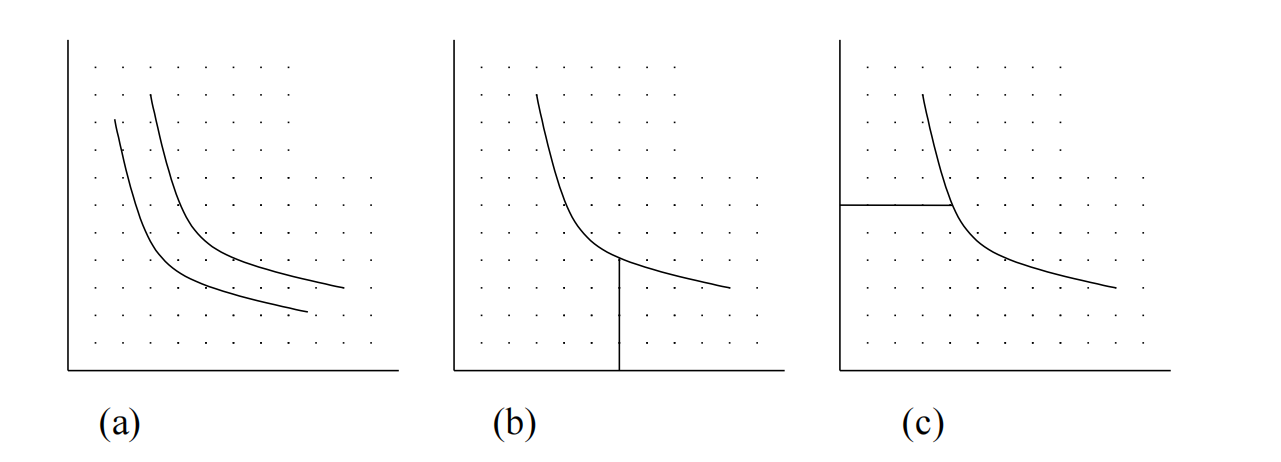
\includegraphics[width=0.9\linewidth]{figure/P4/双曲}
\end{center}

下面把双曲求和用于实 Dirichlet 特征。设 $\chi$ 是非平凡的实
Dirichlet 特征，令
\[
F(m,n)=\frac{\chi(n)}{\sqrt{mn}},
\qquad
S_N=\sum_{mn\leq N}F(m,n).
\]

\begin{proposition}\label{prop:hyperbola-sum-two-estimates}
	存在常数 $c>0$，使得
	\begin{enumerate}[label=\textup{(\roman*)}]
		\item $S_N\geq c\log N$；
		\item
		\[
		S_N=2\sqrt N\,L(1,\chi)+O(1).
		\]
	\end{enumerate}
\end{proposition}

若反设 $L(1,\chi)=0$，则 \textup{(ii)} 给出 $S_N=O(1)$，与
\textup{(i)} 矛盾。因此该命题将完成实特征情形的证明。

首先沿双曲线求和：
\[
\sum_{mn=k}\frac{\chi(n)}{\sqrt{mn}}
=\frac1{\sqrt k}\sum_{n\mid k}\chi(n).
\]

\begin{lemma}\label{lem:real-character-divisor-sum-positive}
	若 $\chi$ 是实 Dirichlet 特征，则对任意正整数 $k$，
	\[
	\sum_{n\mid k}\chi(n)\geq0.
	\]
	若 $k=\ell^2$ 是完全平方数，则
	\[
	\sum_{n\mid k}\chi(n)\geq1.
	\]
\end{lemma}

\begin{proof}
	先设 $k=p^a$。由完全可乘性，
	\[
	\sum_{n\mid p^a}\chi(n)
	=1+\chi(p)+\chi(p)^2+\cdots+\chi(p)^a.
	\]
	由于 $\chi(p)\in\{0,1,-1\}$，右边等于
	\[
	\begin{cases}
		a+1,&\chi(p)=1,\\
		1,&\chi(p)=-1\text{ 且 }a\text{ 为偶数},\\
		0,&\chi(p)=-1\text{ 且 }a\text{ 为奇数},\\
		1,&\chi(p)=0.
	\end{cases}
	\]
	一般地，若 $k=p_1^{a_1}\cdots p_r^{a_r}$，则
	\[
	\sum_{n\mid k}\chi(n)
	=\prod_{j=1}^{r}
	\left(1+\chi(p_j)+\chi(p_j)^2+\cdots+\chi(p_j)^{a_j}\right).
	\]
	每个因子均非负；若 $k$ 是平方数，则每个 $a_j$ 都是偶数，
每个因子至少为 $1$。
\end{proof}

由此，
\[
S_N
=\sum_{k\leq N}\frac1{\sqrt k}\sum_{n\mid k}\chi(n)
\geq\sum_{\ell^2\leq N}\frac1\ell
\geq c\log N,
\]
其中最后一个不等式来自命题
\ref{prop:harmonic-sum-asymptotic}。这证明了命题
\ref{prop:hyperbola-sum-two-estimates} 的 \textup{(i)}。

为了证明 \textup{(ii)}，将区域 $mn\leq N$ 分为
\[
\begin{aligned}
I&=\{1\leq m<\sqrt N,\ \sqrt N<n\leq N/m\},\\
II&=\{1\leq m\leq\sqrt N,\ 1\leq n\leq\sqrt N\},\\
III&=\{\sqrt N<m\leq N/n,\ 1\leq n\leq\sqrt N\}.
\end{aligned}
\]

\begin{center}
		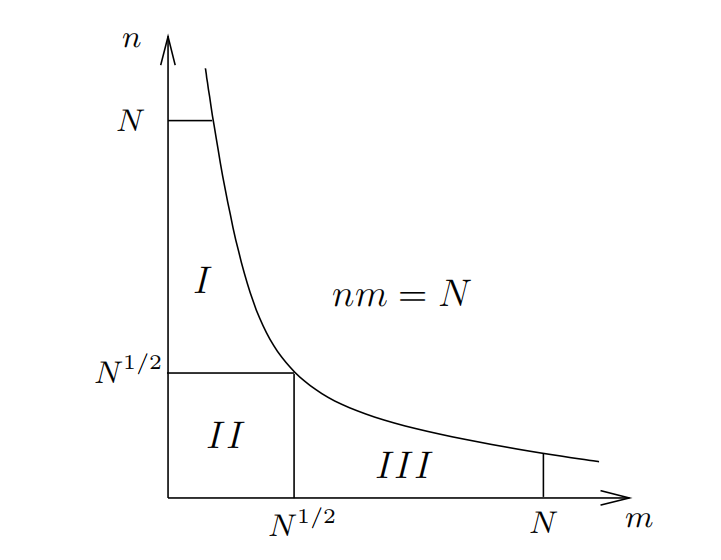
\includegraphics[width=0.7\linewidth]{figure/P4/1,2,3}
\end{center}

分别记这些区域上的和为 $S_I,S_{II},S_{III}$。区域 $I$ 与区域
$III$ 关于 $m=n$ 对称。由于这里的被加函数未必关于 $m,n$ 对称，
在估计时写成
\[
S_N=S_I+(S_{II}+S_{III}),
\]
其中对 $S_I$ 作垂直求和，对 $S_{II}+S_{III}$ 作水平求和。

\begin{lemma}\label{lem:weighted-character-tail-estimates}
	对任意整数 $0<a<b$，有
	\begin{align*}
	\sum_{n=a}^{b}\frac{\chi(n)}{\sqrt n}&=O(a^{-1/2}),\\
	\sum_{n=a}^{b}\frac{\chi(n)}{n}&=O(a^{-1}).
	\end{align*}
\end{lemma}

\begin{proof}
	由引理 \ref{lem:dirichlet-character-partial-sums}，特征的任意部分和
一致有界。对两个和分别作分部求和，并使用微分中值定理，得到
	\[
	\sum_{n=a}^{b}\frac{\chi(n)}{\sqrt n}
	=O\left(\sum_{n=a}^{\infty}n^{-3/2}\right)+O(a^{-1/2})
	=O(a^{-1/2}),
	\]
	第二个估计同理。
\end{proof}

垂直求和给出
\[
\begin{aligned}
S_I
&=\sum_{m<\sqrt N}\frac1{\sqrt m}
\left(
\sum_{\sqrt N<n\leq N/m}\frac{\chi(n)}{\sqrt n}
\right)\\
&=O\left(N^{-1/4}\sum_{m<\sqrt N}\frac1{\sqrt m}\right)
=O(1),
\end{aligned}
\]
其中使用了引理 \ref{lem:weighted-character-tail-estimates} 与命题
\ref{prop:square-root-sum-asymptotic}。

另一方面，水平求和给出
\[
S_{II}+S_{III}
=\sum_{1\leq n\leq\sqrt N}\frac{\chi(n)}{\sqrt n}
\left(
\sum_{m\leq N/n}\frac1{\sqrt m}
\right).
\]
由命题 \ref{prop:square-root-sum-asymptotic}，
\[
\begin{aligned}
S_{II}+S_{III}
&=\sum_{n\leq\sqrt N}\frac{\chi(n)}{\sqrt n}
\left(2\sqrt{\frac Nn}+c
+O\left(\sqrt{\frac nN}\right)\right)\\
&=2\sqrt N\sum_{n\leq\sqrt N}\frac{\chi(n)}n
+c\sum_{n\leq\sqrt N}\frac{\chi(n)}{\sqrt n}
+O\left(N^{-1/2}\sum_{n\leq\sqrt N}1\right).
\end{aligned}
\]
由 $L(1,\chi)=\sum\limits_{n=1}^{\infty}\chi(n)/n$ 与引理
\ref{lem:weighted-character-tail-estimates}，
\[
2\sqrt N\sum_{n\leq\sqrt N}\frac{\chi(n)}n
=2\sqrt N\,L(1,\chi)+O(1).
\]
另外两个和也都是 $O(1)$。因此
\[
S_N=2\sqrt N\,L(1,\chi)+O(1),
\]
证明了命题 \ref{prop:hyperbola-sum-two-estimates} 的 \textup{(ii)}。
于是实特征情形下 $L(1,\chi)\neq0$，定理
\ref{thm:dirichlet-L-nonvanishing-at-one} 得证。

最后，结合定理 \ref{thm:dirichlet-L-nonvanishing-at-one}、命题
\ref{prop:two-logarithms-for-L} 与式
\eqref{eq:dirichlet-prime-sum-decomposition}，可知每个与 $q$ 互素的
剩余类 $\ell$ 都满足
\[
\sum_{p\equiv\ell\pmod q}\frac1p=\infty.
\]
因此形如 $\ell+kq$ 的素数有无穷多个，Dirichlet 定理得证。
%

%\part{实分析}
%\part{泛函分析}
%\part{调和分析}
%\setpartimage{figure/part末封面图.png}
%\setpartintro{这一部分收录一些分散在全笔记中各个部分的一些问题整理出的小短篇。}
%\part*{一些短篇——分析篇}
%
%% ===== 短篇 / 短篇1：Weierstrass第一逼近定理的几种证明 =====
% !TEX root = ../../main.tex
\setchapterimage{figure/Pm/PmA1封面图.png}
\setchapterintro{}
\chapter*{Weierstrass第一逼近定理的几种证明}
% 正文：正文（原文未分节）
% !TEX root = ../../../main.tex
% 所属：短篇 / 短篇1：Weierstrass第一逼近定理的几种证明
% 内容：正文（原文未分节）
% 正文按原文件顺序保存；由 ../article1.tex 调用。
\begin{definition}(Bernstein 多项式)
	$Y$ 是多项式全体构成的集合,定义映射
	\[
	B_n:C[0,1]\longrightarrow Y
	\]
	为
	\[
	f(t)\longmapsto B_n(f,x)=\sum_{k=0}^{n} f\left(\frac{k}{n}\right) C_n^k x^k(1-x)^{n-k}.
	\]
	这里 $B_n(f,x)$ 表示 $f\in X$ 在映射 $B_n$ 作用下的像,它是以 $x$ 为变量的 $n$ 次多项式,称为 $f$ 的 Bernstein 多项式.
\end{definition}

关于映射 $B_n$,直接从定义出发,可以证明它有下述基本性质与基本关系.

对 $B_n$ 有
\begin{enumerate}
	\item $B_n$ 是线性映射,即对任意 $f,g\in X$ 与 $\alpha,\beta\in\mathbb{R}$,成立
	\[
	B_n(\alpha f+\beta g,x)=\alpha B_n(f,x)+\beta B_n(g,x).
	\]
	\item $B_n$ 具有单调性,即若 $f(t)\geqslant g(t)$ 对一切 $t\in[0,1]$ 成立,则
	\[
	B_n(f,x)\geqslant B_n(g,x)
	\]
	对一切 $x\in[0,1]$ 成立.
	\item 对一切 $x\in[0,1]$,成立
	\[
	B_n(1,x)=1,\qquad B_n(t,x)=x,\qquad B_n(t^2,x)=x^2+\frac{x-x^2}{n}.
	\]
	进一步,对任意常数 $s$,有
	\[
	B_n((t-s)^2,x)=\frac{x-x^2}{n}+(x-s)^2.
	\]
\end{enumerate}



\begin{theorem}(Weierstrass 第一逼近定理)\label{weierstrass第一逼近定理}
	设 $f(x)$ 是闭区间 $[a,b]$ 上的连续函数,则对任意给定的 $\varepsilon>0$,存在多项式 $P(x)$,使得
	\[
	|P(x)-f(x)|<\varepsilon
	\]
	对一切 $x\in[a,b]$ 成立.
\end{theorem}
这个证明来自于苏联的Korovkin
\begin{proof}
	一般性地,我们先证 $[a,b]=[0,1]$ 的情形.
	
	由于 $f$ 在 $[0,1]$ 上连续,所以必定有界,即存在 $M>0$,使得对一切 $t\in[0,1]$ 成立
	\[
	|f(t)|\leqslant M.
	\]
	又由 Cantor 定理, $f$ 在 $[0,1]$ 上一致连续.于是对任意给定的 $\varepsilon>0$,存在 $\delta>0$,使得对一切 $t,s\in[0,1]$,当 $|t-s|<\delta$ 时,成立
	\[
	|f(t)-f(s)|<\frac{\varepsilon}{2}.
	\]
	当 $|t-s|\geqslant\delta$ 时,有
	\[
	|f(t)-f(s)|\leqslant 2M\leqslant\frac{2M}{\delta^2}(t-s)^2.
	\]
	也就是说,对一切 $t,s\in[0,1]$,成立
	\[
	-\frac{\varepsilon}{2}-\frac{2M}{\delta^2}(t-s)^2
	\leqslant f(t)-f(s)\leqslant
	\frac{\varepsilon}{2}+\frac{2M}{\delta^2}(t-s)^2.
	\]
	把上式看作关于 $t$ 的连续函数不等式,并对其作用 $B_n$,由 $B_n$ 的单调性得到对一切 $x,s\in[0,1]$,
	\[
	-\frac{\varepsilon}{2}-\frac{2M}{\delta^2}\left[\frac{x-x^2}{n}+(x-s)^2\right]
	\leqslant B_n(f,x)-f(s)
	\leqslant
	\frac{\varepsilon}{2}+\frac{2M}{\delta^2}\left[\frac{x-x^2}{n}+(x-s)^2\right].
	\]
	令 $s=x$,并注意到 $x(1-x)\leqslant\dfrac14$,即得
	\[
	\left|\sum_{k=0}^{n} f\left(\frac{k}{n}\right)C_n^k x^k(1-x)^{n-k}-f(x)\right|
	\leqslant \frac{\varepsilon}{2}+\frac{M}{2n\delta^2}.
	\]
	取
	\[
	N=\left[\frac{M}{\delta^2\varepsilon}\right]+1,
	\]
	当 $n>N$ 时,有
	\[
	\left|\sum_{k=0}^{n} f\left(\frac{k}{n}\right)C_n^k x^k(1-x)^{n-k}-f(x)\right|<\varepsilon
	\]
	对一切 $x\in[0,1]$ 成立.而左边的求和正是多项式 $B_n(f,x)$ 与 $f(x)$ 的差.
	
	一般闭区间 $[a,b]$ 的情形,只需对区间作线性变换化为 $[0,1]$ 即可.
\end{proof}

\begin{proposition}(Weierstrass 定理的序列形式)\label{weierstrass序列形式}
	如果 $f$ 是 $[a,b]$ 上的一个连续函数,那么存在多项式 $P_n$ 的序列,使得
	\[
	\lim_{n\to\infty}P_n(x)=f(x)
	\]
	在 $[a,b]$ 上一致地成立.如果 $f$ 是实函数,那么 $P_n$ 可以取为实多项式.
\end{proposition}

\begin{proof}
	由定理\ref{weierstrass第一逼近定理},取 $\varepsilon=\dfrac1n$,则存在多项式 $P_n(x)$,使得对一切 $x\in[a,b]$,
	\[
	|P_n(x)-f(x)|<\frac1n.
	\]
	于是 $P_n\rightrightarrows f$ 于 $[a,b]$.
	
	反过来,若已经有多项式列 $P_n\rightrightarrows f$,则对任意 $\varepsilon>0$,存在 $N$,使得当 $n>N$ 时
	\[
	\sup_{x\in[a,b]}|P_n(x)-f(x)|<\varepsilon.
	\]
	取 $P=P_{N+1}$,便得到定理\ref{weierstrass第一逼近定理} 的形式.
\end{proof}

下面给出定理\ref{weierstrass序列形式} 的另一种证明,也就是 Rudin 中的证明方法.

\begin{proof}[另一种证明]
	仍不妨设 $[a,b]=[0,1]$.还可以假定 $f(0)=f(1)=0$. 因为若一般情形已经化为这种情形,只需考虑
	\[
	g(x)=f(x)-f(0)-x[f(1)-f(0)],\qquad 0\leqslant x\leqslant 1.
	\]
	则 $g(0)=g(1)=0$,而 $f-g$ 是一次函数,所以 $g$ 若为一致收敛多项式列的极限,则 $f$ 也是.
	
	在 $[0,1]$ 以外的点上定义 $f(x)=0$,则 $f$ 在整个实轴上一致连续.令
	\[
	Q_n(x)=c_n(1-x^2)^n\qquad (n=1,2,3,\cdots),
	\]
	其中 $c_n$ 由下式确定:
	\[
	\int_{-1}^{1}Q_n(x)\dd x=1.
	\]
	于是
	\[
	\frac1{c_n}=\int_{-1}^{1}(1-x^2)^n\dd x
	\geqslant \int_{-1/\sqrt n}^{1/\sqrt n}(1-x^2)^n\dd x
	\geqslant \int_{-1/\sqrt n}^{1/\sqrt n}(1-nx^2)\dd x
	=\frac{4}{3\sqrt n}.
	\]
	从而
	\[
	c_n<\sqrt n.
	\]
	上式中用到的不等式 $(1-x^2)^n\geqslant 1-nx^2$ 是显然的.这说明对任意 $\delta>0$,
	\[
	Q_n(x)\leqslant \sqrt n(1-\delta^2)^n,
	\qquad \delta\leqslant |x|\leqslant 1,
	\]
	于是 $Q_n(x)\to0$ 在 $\delta\leqslant |x|\leqslant1$ 上一致成立.
	
	现在令
	\[
	P_n(x)=\int_{-1}^{1}f(x+t)Q_n(t)\dd t,
	\qquad 0\leqslant x\leqslant1.
	\]
	利用 $f$ 的定义并作变量代换,可得
	\[
	\begin{aligned}
		P_n(x)&=\int_{x-1}^{x+1}f(u)Q_n(u-x)\dd u\\
		&=\int_0^1 f(u)Q_n(u-x)\dd u.
	\end{aligned}
	\]
	由于 $Q_n(u-x)=c_n[1-(u-x)^2]^n$ 关于 $x$ 是多项式,所以 $P_n(x)$ 也是关于 $x$ 的多项式.
	
	给定 $\varepsilon>0$.由 $f$ 的一致连续性,存在 $\delta>0$,使得当 $|t|<\delta$ 时,
	\[
	|f(x+t)-f(x)|<\frac{\varepsilon}{2}
	\]
	对所有 $x$ 成立.记 $M=\max |f|$.由 $\int_{-1}^{1}Q_n(t)\dd t=1$,有
	\[
	\begin{aligned}
		|P_n(x)-f(x)|
		&\leqslant \int_{-1}^{1}|f(x+t)-f(x)|Q_n(t)\dd t\\
		&\leqslant \int_{-\delta}^{\delta}|f(x+t)-f(x)|Q_n(t)\dd t
		+\int_{\delta\leqslant |t|\leqslant1}|f(x+t)-f(x)|Q_n(t)\dd t\\
		&\leqslant \frac{\varepsilon}{2}+2M\int_{\delta\leqslant |t|\leqslant1}Q_n(t)\dd t.
	\end{aligned}
	\]
	而后一项随 $n\to\infty$ 一致趋于 $0$,故对充分大的 $n$,
	\[
	|P_n(x)-f(x)|<\varepsilon
	\]
	对一切 $x\in[0,1]$ 成立.
\end{proof}%

%% ===== 短篇 / 短篇2：关于热方程的若干问题 =====
\setchapterimage{figure/Pm/PmA2封面图.png}
\setchapterintro{}
\chapter*{关于热方程的若干问题}
%\setpartimage{figure/Pt/partt封面图.png}
%\setpartintro{这一部分收录一些分散在全笔记中各个部分的一些特殊函数及其性质。}
%\part*{特殊函数}






	\nocite{*}
	
	\begingroup
	\setlength{\emergencystretch}{1em}
	\markboth{}{}
	\providecommand{\phantomsection}{}
	\defbibheading{normalbib}[\bibname]{%
		\clearpage
		\phantomsection
		\addcontentsline{toc}{chapter}{#1}%
		{\noindent\huge\bfseries #1\par}%
		\vspace{1.5em}%
	}
	
	\printbibliography[
	heading=normalbib,
	title={参考文献}
	]
	
	\endgroup
	
	
\end{document}
